\documentclass[10pt,twoside,onecolumn,openany,final]{memoir}
\setstocksize{10.75in}{8.25in}

\usepackage[toc,lot,lof]{multitoc}
\usepackage[top=.75in, bottom=.75in, left=.75in, right=.75in]{geometry}
\usepackage{graphicx} \graphicspath{{./images/}}
\usepackage{longtable}
\usepackage{mdwlist}
\usepackage{microtype} \DisableLigatures{encoding = *, family = *}
\usepackage{multicol}
\usepackage{textcomp}
\usepackage[normalem]{ulem}
\usepackage{wrapfig}
\usepackage{xtab}
\usepackage{enumerate}
\usepackage{phonetic}
\usepackage{bbding}
\usepackage{linearb}
\usepackage{cypriot}
\usepackage{tipa}
\usepackage{xfrac}
\usepackage{appendix}
\usepackage{xparse}
\usepackage{letltxmacro}
\usepackage{makeidx} \makeindex
\usepackage[table]{xcolor}
\definecolor{offyellow}{RGB}{255,255,128}
\definecolor{links}{RGB}{200,0,50}

%% Font
\usepackage[T1]{fontenc}
\usepackage[bitstream-charter]{mathdesign}
\usepackage{aurical}

\usepackage[colorlinks=true,linkcolor=blue,urlcolor=links,pdfstartview={XYZ null null 1.00},bookmarksdepth=2]{hyperref}
%%%%%%%%%%%%%%%%%%%%%%%%%
%%%% End of Import Section %%%%%%%%%%%
%%%%%%%%%%%%%%%%%%%%%%%%%

%%%%%%%%%%%%%%%%%%%%%%%%%%%%%%%%%%%%%%%%%%%%%%%%%%
%%%%%%%%%%%%%%%%%%%%%%%%%%%%%%%%%%%%%%%%%%%%%%%%%%
%%% Revised Commands
%%%%%%%%%%%%%%%%%%%%%%%%%%%%%%%%%%%%%%%%%%%%%%%%%%
%%%%%%%%%%%%%%%%%%%%%%%%%%%%%%%%%%%%%%%%%%%%%%%%%%
\makeatletter

%fiddles with how chapter titles are displayed
\renewcommand{\@makechapterhead}[1]{%
\vspace*{0 pt}{%
\raggedright \normalfont \fontsize{32}{32} \selectfont \bfseries%
\ifnum \value{secnumdepth}>-1%
  \if@mainmatter \vspace{-8pt} {\fontsize{20}{20} \selectfont Chapter \thechapter:}\\[8pt]%
  \fi%
\fi
\hspace{0.65cm} #1\par\nobreak\vspace{20 pt}%
}}

%makes paragraphs show up closer together
\renewcommand{\paragraph}{%
\@startsection{paragraph}{4}%
{\z@}{1.0ex \@plus 1ex \@minus 0.2ex}{-1em} % wtf is an 'ex' anyways?
{\normalfont\normalsize\bfseries}%
}

%lets multicolumn have the proper background colors as defined by rowcolors
\let\oldmc\multicolumn
\newcommand{\mcinherit}{% Activate \multicolumn inheritance
  \renewcommand{\multicolumn}[3]{%
    \oldmc{##1}{##2}{\ifodd\rownum \@oddrowcolor\else\@evenrowcolor\fi ##3}%
  }}

\makeatother

%add labels within sections, subsections, and subsubsections
\LetLtxMacro{\oldsection}{\section}
\renewcommand{\section}[1]{\oldsection{#1}\label{sec:#1}}

\LetLtxMacro{\oldsubsection}{\subsection}
\renewcommand{\subsection}[1]{\oldsubsection{#1}\label{sec:#1}}

\LetLtxMacro{\oldsubsubsection}{\subsubsection}
\renewcommand{\subsubsection}[1]{\oldsubsubsection{#1}\label{sec:#1}}

%only put chapters and sections into the TOC
\setcounter{secnumdepth}{1}
%makes a subsubsection start off indented.
\setlength{\beforesubsubsecskip}{-\beforesubsubsecskip}

%%%%%%%%%%%%%%%%%%%%%%%%%%%%%%%%%%%%%%%%%%%%%%%%%%
%%%%%%%%%%%%%%%%%%%%%%%%%%%%%%%%%%%%%%%%%%%%%%%%%%
%%% New Commands
%%%%%%%%%%%%%%%%%%%%%%%%%%%%%%%%%%%%%%%%%%%%%%%%%%
%%%%%%%%%%%%%%%%%%%%%%%%%%%%%%%%%%%%%%%%%%%%%%%%%%
\newcommand{\tagline}[1]{\vspace{-6pt} \textit{#1} \medskip}

\newcommand{\gameterm}[1]{#1\index{#1}}

\newcommand{\raceentry}[1]{\oldsection{#1}\index{#1 (race)}\label{race:#1}}

\newcommand{\classentry}[1]{\oldsection{#1}\index{#1 (class)}\label{class:#1}}
\newcommand{\Requirements}{\oldsubsubsection*{Requirements}}
\newcommand{\Basics}{\oldsubsubsection*{Basics}}
\newcommand{\ClassFeatures}{\oldsubsubsection*{Class Features}}

\newcommand{\skillentry}[2]{\oldsubsection[#1]{#1 #2}\index{#1 (skill)}\label{skill:#1}}

\NewDocumentCommand\featentry{m+g}{%
  \IfNoValueTF{#2}
    {\oldsubsubsection[#1]{#1 [General]}\label{feat:#1}}%no second arg, general feat
    {\oldsubsubsection[#1]{#1 [#2]}\label{feat:#1}}%second arg, special type of feat
}

\newcommand{\spellentry}[1]{\oldsubsubsection{#1}\label{spell:#1}}

\NewDocumentCommand\linkrace{m+g}{%
  \IfNoValueTF{#2}
    {\hyperref[race:#1]{#1}}%no second arg, display is same as link
    {\hyperref[race:#1]{#2}}%second arg, link to first and display second
}
\NewDocumentCommand\linkclass{m+g}{%
  \IfNoValueTF{#2}
    {\hyperref[class:#1]{#1}}%no second arg, display is same as link
    {\hyperref[class:#1]{#2}}%second arg, link to first and display second
}
\NewDocumentCommand\linkskill{m+g}{%
  \IfNoValueTF{#2}
    {\hyperref[skill:#1]{#1}}%no second arg, display is same as link
    {\hyperref[skill:#1]{#2}}%second arg, link to first and display second
}
\NewDocumentCommand\linkfeat{m+g}{%
  \IfNoValueTF{#2}
    {\hyperref[feat:#1]{#1}}%no second arg, display is same as link
    {\hyperref[feat:#1]{#2}}%second arg, link to first and display second
}
\NewDocumentCommand\linkspell{m+g}{%
  \IfNoValueTF{#2}
    {\hyperref[spell:#1]{#1}}%no second arg, display is same as link
    {\hyperref[spell:#1]{#2}}%second arg, link to first and display second
}
\NewDocumentCommand\linkcondition{m+g}{%
  \IfNoValueTF{#2}
    {\hyperref[condition:#1]{#1}}%no second arg, display is same as link
    {\hyperref[condition:#1]{#2}}%second arg, link to first and display second
}
\NewDocumentCommand\linkability{m+g}{%
  \IfNoValueTF{#2}
    {\hyperref[ability:#1]{#1}}%no second arg, display is same as link
    {\hyperref[ability:#1]{#2}}%second arg, link to first and display second
}
\NewDocumentCommand\linksec{m+g}{%
  \IfNoValueTF{#2}
    {\hyperref[sec:#1]{#1}}%no second arg, display is same as link
    {\hyperref[sec:#1]{#2}}%second arg, link to first and display second
}

\begin{document}

%%%%%%%%%%%%%%%%%%%%%%%%%%%%%%%%%%%%%%%%%%%%%%%%%%
%%%%%%%%%%%%%%%%%%%%%%%%%%%%%%%%%%%%%%%%%%%%%%%%%%
%%% Title Page
%%%%%%%%%%%%%%%%%%%%%%%%%%%%%%%%%%%%%%%%%%%%%%%%%%
%%%%%%%%%%%%%%%%%%%%%%%%%%%%%%%%%%%%%%%%%%%%%%%%%%
\thispagestyle{empty}
\begin{center}
\textsc{\Large}\\[0.25cm]
\rule{\linewidth}{0.5mm} \\[0.70cm]
\fontsize{30}{30} \selectfont System Reference Document PDF\\[.30cm]
\fontsize{16}{18} \selectfont \guillemotleft{} For that game we all known and love \guillemotright{}\\
\rule{\linewidth}{0.5mm} \\[0.6cm]
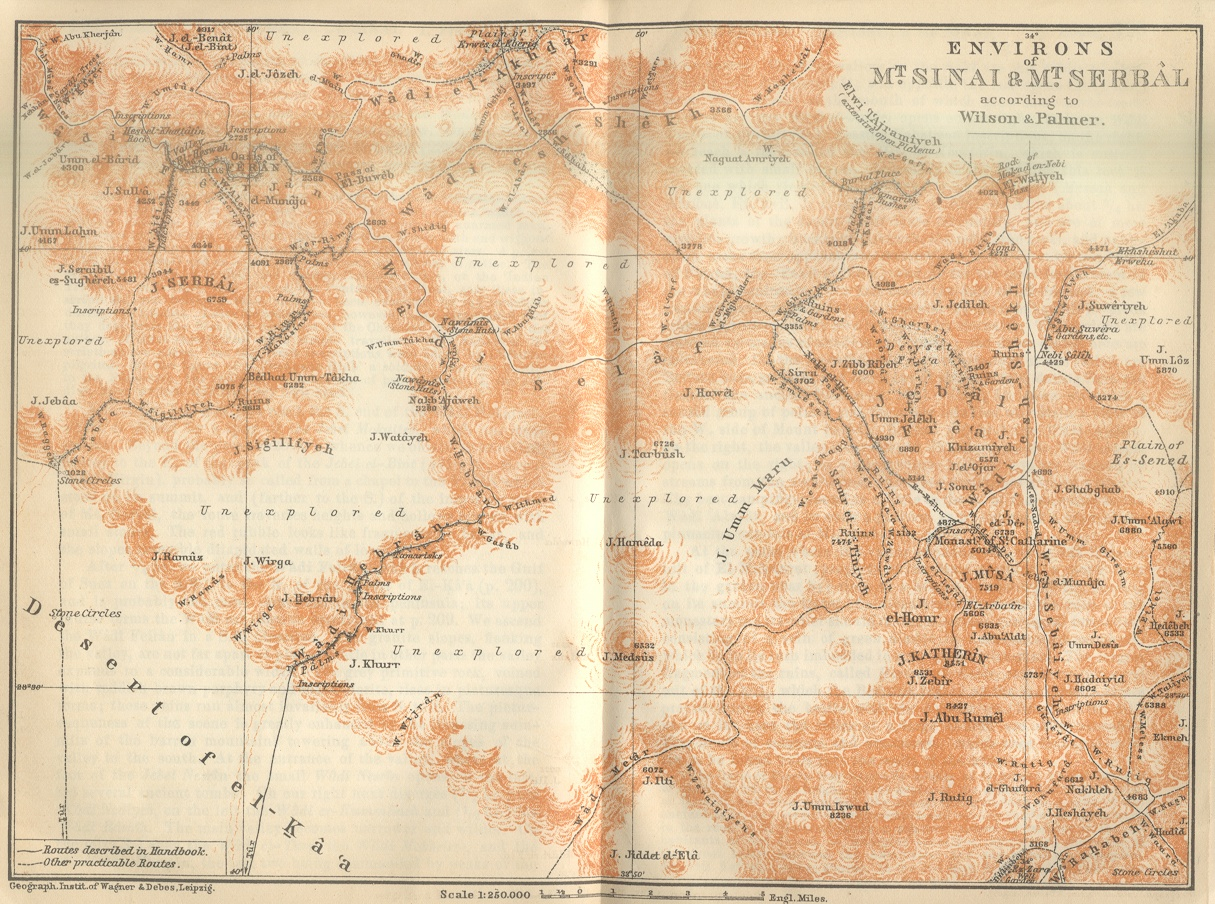
\includegraphics[clip,trim=5cm 2cm 9cm 1cm,width=\linewidth]{images/OldBookArt--MapImages-173.jpg}
\vfill
{\large \textit{This material is Open Game Content, and is licensed for public use under the terms of the Open Game License v1.0a.}\\
\today}
\end{center}

\pagebreak
\sffamily
\pagestyle{plain}
\raggedbottom

%%%%%%%%%%%%%%%%%%%%%%%%%%%%%%%%%%%%%%%%%%%%%%%%%%
%%%%%%%%%%%%%%%%%%%%%%%%%%%%%%%%%%%%%%%%%%%%%%%%%%
%%% Table of Contents
%%%%%%%%%%%%%%%%%%%%%%%%%%%%%%%%%%%%%%%%%%%%%%%%%%
%%%%%%%%%%%%%%%%%%%%%%%%%%%%%%%%%%%%%%%%%%%%%%%%%%
\renewcommand{\contentsname}{Table of Contents}
\setcounter{tocdepth}{1}
\tableofcontents

%%%%%%%%%%%%%%%%%%%%%%%%%%%%%%%%%%%%%%%%%%%%%%%%%%
%%%%%%%%%%%%%%%%%%%%%%%%%%%%%%%%%%%%%%%%%%%%%%%%%%
%%% Main Content
%%%%%%%%%%%%%%%%%%%%%%%%%%%%%%%%%%%%%%%%%%%%%%%%%%
%%%%%%%%%%%%%%%%%%%%%%%%%%%%%%%%%%%%%%%%%%%%%%%%%%

%% Primary Chapters Here

\clearpage
\chapter{Introduction}
\section{What is a Role-playing Game?}
foo
\section{What You Need To Play}
foo
\section{The Core Mechanic}
foo
\section{Creating a Character}
foo
%%%%%%%%%%%%%%%%%%%%%%%%
%%Race Chapter Formatting
%%%%%%%%%%%%%%%%%%%%%%%%
\newcommand{\race}{placeholder}

\newcommand{\racedescription}[1]{\indent\ability{Physical Description}{#1}}
\newcommand{\racepersonality}[1]{\indent\ability{Personality}{#1}}
\newcommand{\racesociety}[1]{\indent\ability{Society}{#1}}
\newcommand{\racealignment}[1]{\indent\ability{Alignment}{#1}}

\newcommand{\type}[1]{\ability{Type}{#1}\\}
\newcommand{\size}[1]{\ability{Size}{#1}\\}
\newcommand{\speed}[1]{\ability{Speed}{#1 feet}\\}
\newcommand{\scores}[1]{\ability{Racial Ability Score Modifiers}{#1}\\}
\newcommand{\racialtraits}[1]{\ability{Unique Racial Traits}{#1}\\}
\newcommand{\racetrait}[2]{\newline\textbullet{ \ability{#1}{#2}}}
\newcommand{\senses}[1]{\ability{Senses}{#1}\\}
\newcommand{\autolanguages}[1]{\ability{Automatic Languages}{#1}\\}
\newcommand{\bonuslanguages}[1]{\ability{Bonus Languages}{#1}\\}
\newcommand{\favoredclasses}[1]{\ability{Favored Classes}{#1}\\}
\newcommand{\male}[4]{Male &#1 &#2 &#3 &#4\\}
\newcommand{\female}[4]{Female &#1 &#2 &#3 &#4\\}

\newenvironment{racetable}
{
\tabulinesep=1mm
\noindent
\begin{tabu} to \columnwidth {X}
\header\textbf{\race ~Racial Traits} \\ \hline
\end{tabu}
\vspace{-.1em}
\rowcolors{1}{colortwo}{colorone}
\begin{tabu} to \columnwidth {X [1, l]}
}{
\hline
\end{tabu}
}

\newcommand{\agetable}[4]{
\tabulinesep=1mm
\noindent
\begin{tabu} to \columnwidth {X}
\header\textbf{\race ~Starting Age} \\ \hline
\end{tabu}
\vspace{-.15em}
\rowcolors{1}{colortwo}{colorone}
\begin{tabu} to \columnwidth {X X X X}
\textbf{Adulthood:} &\textbf{Simple:} &\textbf{Moderate:} &\textbf{Complex:} \\
#1 Years &#2 &#3 &#4 \\ \hline
\end{tabu}
}

\newenvironment{heightweighttable}
{
\tabulinesep=1mm
\noindent
\begin{tabu} to \columnwidth {X}
\header\textbf{\race ~Height and Weight} \\ \hline
\end{tabu}
\vspace{-.5em}
\rowcolors{1}{colortwo}{colorone}
\begin{tabu} to \columnwidth {X X X X X}
\textbf{Gender} &\textbf{Base Height} &\textbf{Height Mod.} &\textbf{Base Weight} &\textbf{Weight Mod.} \\
}{
\hline
\end{tabu}
}

\newenvironment{raceleft}
{
\vspace{0pt}
\begin{minipage}[t]{0.5\linewidth}
}{
\end{minipage}
}

\newenvironment{raceright}
{\begin{minipage}[t]{0.5\linewidth}
\vspace{0pt}
}{
\end{minipage}
}

\newenvironment{racebox}
{
\vspace{0pt}
%\nointerlineskip
\begin{minipage}[t][0.49\textheight][t]{\textwidth}
}{
\end{minipage}
}


\chapter{Races}

\raceentry{Aasimar}{``My ancestors were more beautiful than you can imagine."}\\
\begin{multicols}{2}
Aasimar are humans that have a beautiful outsider, usually but not always a celestial, somewhere in their ancestry. \linebreak
\indent\textbf{Personality: }Though mostly human, an aasimar's immortal heritage influences their mental development. Aasimar tend toward more extreme personalities, being especially quiet and introspective or particularly loud and boisterous. Most aasimar are very opinionated, and have strongly held beleifs.\linebreak
\indent\textbf{Physical Description: }Aasimar look like especially beautiful humans, though they sometimes bear vestiges of their ancestry that denote them as being different (strangely colored eyes, silver-blonder or white hair, slightly `off' facial features).\linebreak
\indent\textbf{Society: }Aasimar are typically born and raised in human societies, and gain the same customs of that culture.\linebreak
\indent\textbf{Alignment: }Most aasimar are the descendants of celestials, and tend towards the good alignments. Rarely, an aasimar might instead have an infernal heritage, being the descendant of an erinyes or succubus. Such aasimar instead tend towards an evil alignment.\linebreak

\columnbreak

\racetable
\type{Outsider (Native and Human Subtype)}
\size{Medium}
\speed{30 foot}
\standardsenses
\scores{+2 Wisdom, +2 Charisma}
\racespecial{
\fakeitem{\spell{Light} \sla : An Aasimar with a Charisma of at least 10 may cast \spell{light} as a spell-like ability with a caster level equal to their character level once per day.} \linebreak
\fakeitem{+2 bonus to Spot, and Listen checks.}
}
\autolanguages{Common}
\bonuslanguages{Abyssal, Aquan, Auran, Celestial, Formian, Ignan, Slaad, Sylvan, Terran.}
\favoredclasses{Paladin and Sorcerer}
\end{tabu}

\vspace{\baselineskip}
\agetable{20}{+1d6}{+2d6}{+3d6}

\vspace{\baselineskip}
\male{4' 7"}{+2d8}{90 lb.}{x(2d4)}
\female{4' 5"}{+2d8}{80 lb.}{x(2d4)}
\heightweighttable
\end{multicols}

\begin{racebox}
\raceentry{Drow}{``Time to die for the Spider Queen."}
\begin{multicols}{2}

\begin{racetable}
\type{Humanoid (Elf Subtype)}
\size{Medium}
\scores{+2 Dexterity, -2 Constitution}
\speed{30}
\senses{Darkvision 120'}
\autolanguages{Elvish}
\bonuslanguages{Abyssal, Beholder, Common, Draconic, Drow Sign Language, Dwarvish, Gnome, Kuo-Toa, Terran, Undercommon}
\favoredclasses{Cleric and Wizard}
\end{racetable}

\vspace{\baselineskip}
\agetable{20}{+1d6}{+2d6}{+3d6}

\vspace{\baselineskip}
\begin{heightweighttable}
\male{4' 7"}{+2d8}{90 lb.}{x(2d4)}
\female{4' 5"}{+2d8}{80 lb.}{x(2d4)}
\end{heightweighttable}

\racialtraits{
\racetrait{Daylight Sensitivity}{While in brightly lit surroundings (such as a daylight spell), a Drow suffers a -2 penalty to attack rolls and precision-based skill checks.}
\racetrait{Innate Magic}{Drow with a Charisma of at least 10 may cast deeper darkness (duration 4 hours), and fairie fire as spell-like abilities with a caster level equal to their character level once per day each.}
\racetrait{Magic Resistant}{+2 bonus to saving throws against spells and spell-like abilities.}
\racetrait{Skill Bonus}{+2 bonus to Spot and Listen checks.}
\racetrait{Elven Trance}{Drow never sleep and are immune to sleep effects. Drow must still perform their 4 hour daily trance to stay coherent and rested.}
\racetrait{Interesting Times}{Drow live an exceedingly interesting life and every Drow has proficiency with the rapier and an exotic ranged weapon of their choice.}
}

\end{multicols}
\end{racebox}

\raceentry{Dwarf}
\quot{``I remember that...''}

\listone
		\item Medium Size
		\item 20' movement
		\item Humanoid Type (Dwarf Subtype)
		\item +2 Constitution, -2 Charisma
		\item Dwarves can move up to their full speed even when wearing medium or heavy armor or when carrying a medium or heavy load
		\item Darkvision: Dwarves can see up to 60 feet in the dark.
		\item Stonecunning: This ability grants a dwarf a +2 racial bonus on Search checks to notice unusual stonework, such as sliding walls, stonework traps, new construction (even when built to match the old), unsafe stone surfaces, shaky stone ceilings, and the like. Something that isn’t stone but that is disguised as stone also counts as unusual stonework. A dwarf who merely comes within 10 feet of unusual stonework can make a Search check as if he were actively searching, and a dwarf can use the Search skill to find stonework traps as a rogue can. A dwarf can also intuit depth, sensing his approximate depth underground as naturally as a human can sense which way is up.
		\item Weapon Familiarity: Dwarves may treat dwarven waraxes and dwarven urgroshes as martial weapons, rather than exotic weapons.
		\item Stability: A dwarf gains a +4 bonus on ability checks made to resist being bull rushed or tripped when standing on the ground (but not when climbing, flying, riding, or otherwise not standing firmly on the ground).
		\item +2 racial bonus on saving throws against poison.
		\item +2 racial bonus on saving throws against spells and spell-like effects.
		\item +1 racial bonus on attack rolls against orcs and goblinoids.
		\item +4 dodge bonus to Armor Class against monsters of the giant type. Any time a creature loses its Dexterity bonus (if any) to Armor Class, such as when it’s caught flat-footed, it loses its dodge bonus, too.
		\item +2 racial bonus on Appraise checks that are related to stone or metal items.
		\item +2 racial bonus on Craft checks that are related to stone or metal.
		\item Favored class: Fighter
		\item Automatic Languages: Common and Dwarven.
		\item Bonus Languages: Giant, Gnome, Goblin, Orc, Terran, and Undercommon.
\end{list}


\raceentry{Elf}
\quot{``You shall never harm my beautiful trees!''}

\listone
		\item Medium Size
		\item Humanoid Type (Elf Subtype)
		\item 30' movement
		\item +2 Dexterity, -2 Constitution
		\item Low Light Vision: Elves can see twice as far as a human in poor lighting.
		\item Weapon Proficiency: Elves are proficient with the longsword, rapier, longbow (including composite longbow), and shortbow (including composite shortbow).
		\item +2 racial bonus on Listen, Search, and Spot checks. An elf who merely passes within 5 feet of a secret or concealed door is entitled to a Search check to notice it as if she were actively looking for it.
		\item Favored Class: Wizard.
		\item Automatic Languages: Common and Elven. 
		\item Bonus Languages: Draconic, Gnoll, Gnome, Goblin, Orc, and Sylvan.
\end{list}

\raceentry{Feytouched}
\quot{``All my life, I have never fit in. Not in town, not in the forest. In some integral fashion I am unlike those around me, and I believe it is my fate to live and die alone."}

\listone
		\item Medium Size
    \item Fey Type
    \item 30' movement
    \item Low-Light Vision: Feytouched can twice as far as a human in poor lighting.
    \item +2 Dexterity, +2 Charisma, -2 Constitution. Feytouched are graceful and those which are not beautiful are terrifying, but they are fragile like flowers.
    \item Immunity to [Compulsion] Effects
    \item Magic Affinity: Every Feytouched is different, and marked by the signature magics of the fey in a different manner. Every Feytouched has one spell that can be used once per day as a spell-like ability. This spell is chosen at 1st level and cannot be changed. Any 1st level Illusion or Enchantment spell from the Sorcerer/Wizard list is fair game, and the save DC is Charisma-based.
    \item Favored Class: Bard
    \item Feytouched speak Common and Sylvan. Bonus Languages may be selected from the following list:
      Aquan, Auran, Elvish, Draconic, Dwarvish, Druidic, Goblin, Gnoll, Gnome, Halfling.
\end{list}

\begin{racebox}
\raceentry{Gnome}{``What's that you say little mole? Kobolds in the well!?"}
\begin{multicols}{2}

\begin{racetable}
\type{Humanoid (Gnome subtype)}
\size{Small}
\scores{+2 Constitution, --2 Strength}
\speed{20}
\senses{Low Light Vision}
\autolanguages{Common and Gnome}
\bonuslanguages{Draconic, Dwarven, Elven, Giant, Goblin, and Orc. In addition, a gnome can speak with a burrowing mammal (a badger, fox, rabbit, or the like).}
\favoredclasses{Bard}
\end{racetable}

Nothing until we find or write it.

\racedescription{NYW}

\racepersonality{NYW}

\racesociety{NYW}

\racealignment{NYW}

\racialtraits{
\racetrait{Weapon Familiarity}{Gnomes may treat gnome hooked hammers as martial weapons rather than exotic weapons.}
\racetrait{+2 racial bonus on saving throws against illusions.}
\racetrait{Add +1 to the Difficulty Class for all saving throws against illusion spells cast by gnomes. This adjustment stacks with those from similar effects.}
\racetrait{+1 racial bonus on attack rolls against kobolds and goblinoids.}
\racetrait{+4 dodge bonus to Armor Class against monsters of the giant type.}
\racetrait{+2 racial bonus on Listen checks.}
\racetrait{+2 racial bonus on Craft (alchemy) checks.}
\racetrait{Spell-Like Abilities: 1/day—speak with animals (burrowing mammal only, duration 1 minute). A gnome with a Charisma score of at least 10 also has the following spell-like abilities: 1/day—dancing lights, ghost sound, prestidigitation. Caster level 1st; save DC 10 + gnome’s Cha modifier + spell level.} % I'm pretty sure there's a much better way to format this, say by using the \sla used for aasimar. That Cha req goofs it up.
}


%\columnbreak

\vspace{\baselineskip}
\agetable{40}{+4d6}{+6d6}{+9d6}

\vspace{\baselineskip}
\begin{heightweighttable}
\male{3' 0"}{+2d4}{40 lb.}{x(1)}
\female{2' 10"}{+2d4}{35 lb.}{x(1)}
\end{heightweighttable}
\end{multicols}
\end{racebox}

\raceentry{Goblin}
\quot{``You weren't hired to think. You were hired because you have opposable thumbs."}

\listone
    \item Small Size
    \item 30' movement (despite small size).
    \item Humanoid Type (Goblinoid subtype)
    \item Darkvision: Goblins can see up to 60 feet in the dark.
    \item +2 Dexterity, -2 Strength, -2 Charisma
    \item +4 bonus to Move Silently and Ride checks.
    \item Bonus Feat: Mounted Combat
    \item Goblins benefit from an ancient pact with the Worgs, and every Goblin receives a +2 bonus to any Bluff, Diplomacy, Handle Animal, Sense Motive, or Survival check made with respect to a Worg.
    \item Favored Classes: Rogue and Wizard
    \item Automatic Languages: Common, Goblin
    \item Bonus Languages: Draconic, Elvish, Dwarvish, Giant, Gnoll, Infernal, Orcish, Undercommon, and Worg.
\end{list}
\raceentry{Half-Elf}
\quot{``I don't fit in anywhere, please, listen to me cry.''}

\listone
		\item Medium Size
		\item 30' Movement
		\item Humanoid Type
		\item Low-Light Vision: Half-Elves can see twice as humans in poor lighting.
		\item Immunity to sleep spells and similar magical effects, and a +2 racial bonus on saving throws against enchantment spells or effects.
		\item +1 racial bonus on Listen, Search, and Spot checks.
		\item +2 racial bonus on Diplomacy and Gather Information checks.
		\item Elven Blood: For all effects related to race, a half-elf is considered an elf.
		\item Favored Class: Any
		\item Automatic Languages: Common and Elven.
		\item Bonus Languages: Any (other than secret languages, such as Druidic).
\end{list}
\subsection{Halfling}
\quot{``Where are we going Mr. Frodo?''}

\listone
		\item Small Size
		\item 20' movement
		\item +2 Dexterity, -2 Strength
		\item +2 racial bonus on Climb, Jump, Listen, and Move Silently checks.
		\item +1 racial bonus on all saving throws.
		\item +2 morale bonus on saving throws against fear: This bonus stacks with the halfling’s +1 bonus on saving throws in general.
		\item +1 racial bonus on attack rolls with thrown weapons and slings.
		\item Favored Class: Rogue
		\item Automatic Languages: Common and Halfling.
		\item Bonus Languages: Dwarven, Elven, Gnome, Goblin, and Orc.
\end{list}		

\raceentry{Half-Orc}
\quot{``I don't fit in anywhere, but you may be surprised to know that this dagger fits all kinds of places."}

\listone
    \item Medium Size
    \item 30' movement
    \item Humanoid Type (Orc and Human subtype)
    \item Darkvision: Half-Orcs can see up to 60 feet in the dark.
    \item +2 Strength
    \item +2 to Intimidate, Gather Information, and Survival checks.
    \item Favored Classes: Assassin and Barbarian
    \item Automatic Languages: Orc, Common
    \item Bonus Languages: Any.
\end{list}
\raceentry{Hobgoblin}
\quot{``That's some tough talk from a man who wears a basket on his head."}

\listone
    \item Medium Size
    \item 30' movement.
    \item Humanoid Type (Goblinoid subtype)
    \item Darkvision: Hobgoblins can see up to 60 feet in the dark.
    \item +2 Dexterity, +2 Constitution
    \item +4 bonus to Move Silently checks.
    \item Favored Classes: Fighter and Samurai
    \item Automatic Languages: Common, Goblin
    \item Bonus Languages: Draconic, Elvish, Dwarvish, Giant, Gnoll, Ignan, Infernal, Orcish.
\end{list}
\raceentry{Human}
\quot{``Yeah, I'm pretty normal.''}

\listone
	\item Medium Size
	\item 30' movement.
	\item Humanoid Type (Human subtype)
	\item 1 extra feat at 1st level.
	\item 4 extra skill points at 1st level and 1 extra skill point at each additional level.
	\item Favored Class: Any. When determining whether a multiclass human takes an experience point penalty, his or her highest-level class does not count.
	\item Automatic Language: Common. 
	\item Bonus Languages: Any (other than secret languages, such as Druidic). See the Speak Language skill.
\end{list}
\raceentry{Kobold}
\quot{``Aieeeeeeeee!''}

\listone
		\item Small Size
		\item 30' movement (despite small size)
		\item Humanoid Type (Reptilian subtype)
		\item Darkvision: Kobolds can see up to 60 feet in the dark.
		\item -4 Strength, +2 Dexterity, -2 Constitution
		\item Racial Skills: A kobold character has a +2 racial bonus on Craft (trapmaking), Profession (miner), and Search checks.
		\item +1 natural armor bonus.
		\item Light sensitivity: Kobolds are dazzled in bright sunlight or within the radius of a daylight spell. 
		\item Favored Class: Sorcerer.
		\item Automatic Languages: Draconic.
		\item Bonus Languages: Common, Undercommon.
\end{list}
\raceentry{Orc}
\quot{``Waaarrrggghhhh!"}

\listone
    \item Medium Size
    \item 30' movement.
    \item Humanoid Type (Orc subtype)
    \item Darkvision: Orcs can see up to 60 feet in the dark.
    \item +4 Strength, -2 Intelligence, -2 Charisma, -2 Wisdom
    \item Daylight Sensitivity: While in brightly lit surroundings (such as a daylight spell), an Orc suffers the dazzled condition and is thus at a -1 penalty to attack rolls and precision-based skill checks.
    \item +2 bonus to saving throws vs. Poison and Disease.
    \item Immunity to ingested poisons.
    \item +2 to Jump and Survival checks.
    \item Favored Classes: Barbarian and Cleric
    \item Automatic Languages: Orc, Common
    \item Bonus Languages: Dwarvish, Elvish, Giant, Gnoll, Goblin, Sylvan, Undercommon.
\end{list}
\raceentry{Tiefling}
\quot{``My ancestors were more evil than you will ever know, but let's see how I compare.''}

\listone
    \item Medium Size
    \item 30' movement.
    \item Outsider Type (Native and Human subtype)
    \item Darkvision: Tieflings can see up to 60 feet in the dark.
    \item +2 Dexterity, +2 Intelligence, -2 Charisma
    \item Tieflings with a Charisma of at least 10 may cast darkness as a spell-like ability with a caster level equal to their character level once per day.
    \item +2 bonus to Bluff, Hide, and Move Silently checks.
    \item Favored Classes: Rogue and True Fiend
    \item Automatic Languages: Common
    \item Bonus Languages: Abyssal, Aquan, Auran, Celestial, Formian, Ignan, Slaad, Sylvan, Terran.
\end{list}
%%%%%%%%%%%%%%%%%%%%%%%%
%%Class Chapter Formatting
%%%%%%%%%%%%%%%%%%%%%%%%

\newcommand{\class}{placeholder}
%Holds the class's name, as defined by \classentry

\newenvironment{classpreamble}{
%\centering
%\rowcolors{1}{colorone}{colortwo}
%\begin{tabu} to \textwidth {X}
}{
%\end{tabu}
}

\newcommand{\desc}[1]{\noindent#1 \\}
\newcommand{\playingaclass}[1]{\indent\ability{Playing a \class : }{#1}\\}
\newcommand{\hitdie}[1]{\indent\ability{Hit Die: }{#1}\\}
\newcommand{\alignment}[1]{\indent\ability{Alignment: }{#1}\\}
\newcommand{\races}[1]{\indent\ability{Races: }{#1}\\}
\newcommand{\startinggold}[1]{\indent\ability{Starting Gold: }{#1}\\}
\newcommand{\startingage}[1]{\indent\ability{Starting Age: }{#1}\\}  
\newcommand{\skillpoints}[1]{\indent\ability{Skill Points per Level: }{#1 + Intelligence Bonus}\\}
\newcommand{\classskills}[1]{\newline\indent\ability{Class Skills: }{The {\class}'s class skills (and the key ability for each skill) are #1}\\}

%\newcommand{\desc}[1]{ #1 \\}
%\newcommand{\playingaclass}[1]{\selectfont\ability{Playing a \class : }{#1}\\}
%\newcommand{\hitdie}[1]{\ability{Hit Die: }{#1}\\}
%\newcommand{\alignment}[1]{\ability{Alignment: }{#1}\\}
%\newcommand{\races}[1]{\ability{Races: }{#1}\\}
%\newcommand{\startinggold}[1]{\ability{Starting Gold: }{#1}\\}
%\newcommand{\startingage}[1]{\ability{Starting Age: }{#1}\\}  
%\newcommand{\skillpoints}[1]{\ability{Skill Points per Level: }{#1 + Intelligence Bonus}\\}
%\newcommand{\classskills}[1]{\ability{Class Skills: }{The {\class}'s class skills (and the key ability for each skill) are #1}\\}


\newcommand{\startclassfeatures}{
 \smallskip\noindent All of the following are class features of the \class ~class.}
%place before actual class features entries.

\newcommand{\proficiencies}[1]{
 \ability{Weapon and Armor Proficiencies:}{The \class ~is proficient with #1}}
%Displays proficiencies with minimal input, implimentation looks like \proficiencies{the proficiencies}

\newcommand{\classfeature}[2]{
  \ability{#1}{#2}}
%No functional difference from \ability currently

%%%%Class Table Commands

\newcommand{\gbab}{\empty}
\newcommand{\mbab}{\empty}
\newcommand{\fort}{\empty}
\newcommand{\refl}{\empty}
\newcommand{\will}{\empty}
%Creates new commands for use in \ifx statements for formatting purposes.

\newcommand{\goodbab}{\renewcommand{\gbab}{\empty}\renewcommand{\mbab}{a}}
\newcommand{\modebab}{\renewcommand{\gbab}{a}\renewcommand{\mbab}{\empty}}
\newcommand{\poorbab}{\renewcommand{\gbab}{a}\renewcommand{\mbab}{a}}
%A set of commands to tell LaTeX what BAB progression the class has. Only one should be called per class.

\newcommand{\goodfor}{\renewcommand{\fort}{\empty}}
\newcommand{\poorfor}{\renewcommand{\fort}{a}}
%A set of commands to tell LaTeX what Fortitude progression the class has. Only one should be called per class.

\newcommand{\goodref}{\renewcommand{\refl}{\empty}}
\newcommand{\poorref}{\renewcommand{\refl}{a}}
%A set of commands to tell LaTeX what Reflex progression the class has. Only one should be called per class.

\newcommand{\goodwil}{\renewcommand{\will}{\empty}}
\newcommand{\poorwil}{\renewcommand{\will}{a}}
%A set of commands to tell LaTeX what Will progression the class has. Only one should be called per class.

\newenvironment{classtable}[1]
{
\centering
\rowcolors{1}{colorone}{colortwo}
\begin{tabu} to \textwidth {p{.275in} l p{0.275in} p{0.275in} p{0.275in} X l l l l} 
\rowcolor{headercolor} Level & Base Attack & Fort. & Ref. & Will & Special #1 \\
}{
\hline
\end{tabu}
}
%A a new environment that sets up the class tables. Include the \level commands between \begin{classtable}.

\newenvironment{minorcastingclasstable}
{
%\table[htb]
%\center
\centering
\rowcolors{1}{colorone}{colortwo}
\begin{tabu}to \textwidth{p{.275in}lp{0.275in}p{0.275in}p{0.275in}Xccccccc}
\rowcolor{headercolor} & & & & & &\multicolumn{7}{c}{Spells Per Day (By Level)} \\
\rowcolor{headercolor} Level & Base Attack & Fort. & Ref. & Will & Special &0&1&2&3&4&5&6\\
}{
\hline
\end{tabu}
%\endcenter
%\endtable
}
%A a new environment similar to classtable, but with columns for a minor (zero through six) spell slot progression.

\newenvironment{fullcastingclasstable}
{
\table[htb]
\center
\rowcolors{1}{colorone}{colortwo}
\begin{tabu}to \textwidth{p{.275in}lp{0.275in}p{0.275in}p{0.275in}Xcccccccccc}
\rowcolor{headercolor} & & & & & &\multicolumn{10}{c}{Spells Per Day (By Level)} \\
\rowcolor{headercolor} Level & Base Attack & Fort. & Ref. & Will & Special &0&1&2&3&4&5&6&7&8&9\\
}{
\hline
\end{tabu}
\endcenter
\endtable
}
%Another environment for class tables, this one for full (0 through 9) spell slot progression.

\newcommand{\levelone}[1]{
\hline
1st  & \ifx\gbab\isempty +1 \else\ifx\mbab\isempty +0 \else +0 \fi \fi
	 & \ifx\fort\isempty +2 \else +0 \fi
	 & \ifx\refl\isempty +2 \else +0 \fi
	 & \ifx\will\isempty +2 \else +0 \fi
	 & #1 \\}
%A command that declares a table row within the class feature table.

\newcommand{\leveltwo}[1]{
2nd  & \ifx\gbab\isempty +2 \else\ifx\mbab\isempty +1 \else +1 \fi \fi
	 & \ifx\fort\isempty +3 \else +0 \fi
	 & \ifx\refl\isempty +3 \else +0 \fi
	 & \ifx\will\isempty +3 \else +0 \fi
	 & #1 \\}
%A command that declares a table row within the class feature table.

\newcommand{\levelthree}[1]{
3rd  & \ifx\gbab\isempty +3 \else\ifx\mbab\isempty +2 \else +1 \fi \fi
	 & \ifx\fort\isempty +3 \else +1 \fi
	 & \ifx\refl\isempty +3 \else +1 \fi
	 & \ifx\will\isempty +3 \else +1 \fi
	 & #1 \\}
%A command that declares a table row within the class feature table.

\newcommand{\levelfour}[1]{
4th  & \ifx\gbab\isempty +4 \else\ifx\mbab\isempty +3 \else +2 \fi \fi
	 & \ifx\fort\isempty +4 \else +1 \fi
	 & \ifx\refl\isempty +4 \else +1 \fi
	 & \ifx\will\isempty +4 \else +1 \fi
	 & #1 \\}
%A command that declares a table row within the class feature table.

\newcommand{\levelfive}[1]{
5th  & \ifx\gbab\isempty +5 \else\ifx\mbab\isempty +3 \else +2 \fi \fi
	 & \ifx\fort\isempty +4 \else +1 \fi
	 & \ifx\refl\isempty +4 \else +1 \fi
	 & \ifx\will\isempty +4 \else +1 \fi
	 & #1 \\}
%A command that declares a table row within the class feature table.
	 
\newcommand{\levelsix}[1]{
6th  & \ifx\gbab\isempty +6/+1 \else\ifx\mbab\isempty +4 \else +3 \fi \fi
	 & \ifx\fort\isempty +5 \else +2 \fi
	 & \ifx\refl\isempty +5 \else +2 \fi
	 & \ifx\will\isempty +5 \else +2 \fi
	 & #1 \\}
%A command that declares a table row within the class feature table.

\newcommand{\levelseven}[1]{
7th  & \ifx\gbab\isempty +7/+2 \else\ifx\mbab\isempty +5 \else +3 \fi \fi
	 & \ifx\fort\isempty +5 \else +2 \fi
	 & \ifx\refl\isempty +5 \else +2 \fi
	 & \ifx\will\isempty +5 \else +2 \fi
	 & #1 \\}
%A command that declares a table row within the class feature table.
	 
\newcommand{\leveleight}[1]{
8th  & \ifx\gbab\isempty +8/+3 \else\ifx\mbab\isempty +6/+1 \else +4 \fi \fi
	 & \ifx\fort\isempty +6 \else +2 \fi
	 & \ifx\refl\isempty +6 \else +2 \fi
	 & \ifx\will\isempty +6 \else +2 \fi
	 & #1 \\}
%A command that declares a table row within the class feature table.
	 
\newcommand{\levelnine}[1]{
9th  & \ifx\gbab\isempty +9/+4 \else\ifx\mbab\isempty +6/+1 \else +4 \fi \fi
	 & \ifx\fort\isempty +6 \else +3 \fi
	 & \ifx\refl\isempty +6 \else +3 \fi
	 & \ifx\will\isempty +6 \else +3 \fi
	 & #1 \\}
%A command that declares a table row within the class feature table.
	 
\newcommand{\levelten}[1]{
10th & \ifx\gbab\isempty +10/+5 \else\ifx\mbab\isempty +7/+2 \else +5 \fi \fi
	 & \ifx\fort\isempty +7 \else +3 \fi
	 & \ifx\refl\isempty +7 \else +3 \fi
	 & \ifx\will\isempty +7 \else +3 \fi
	 & #1 \\}
%A command that declares a table row within the class feature table.
	 
\newcommand{\leveleleven}[1]{
11th & \ifx\gbab\isempty +11/+6/+6 \else\ifx\mbab\isempty +8/+3 \else +5 \fi \fi
	 & \ifx\fort\isempty +7 \else +3 \fi
	 & \ifx\refl\isempty +7 \else +3 \fi
	 & \ifx\will\isempty +7 \else +3 \fi
	 & #1 \\}
%A command that declares a table row within the class feature table.
	 
\newcommand{\leveltwelve}[1]{
12th & \ifx\gbab\isempty +12/+7/+7 \else\ifx\mbab\isempty +9/+4 \else +6/+1 \fi \fi
	 & \ifx\fort\isempty +8 \else +4 \fi
	 & \ifx\refl\isempty +8 \else +4 \fi
	 & \ifx\will\isempty +8 \else +4 \fi
	 & #1 \\}
%A command that declares a table row within the class feature table.
	 
\newcommand{\levelthirteen}[1]{
13th & \ifx\gbab\isempty +13/+8/+8 \else\ifx\mbab\isempty +9/+4 \else +6/+1 \fi \fi
	 & \ifx\fort\isempty +8 \else +4 \fi
	 & \ifx\refl\isempty +8 \else +4 \fi
	 & \ifx\will\isempty +8 \else +4 \fi
	 & #1 \\}
%A command that declares a table row within the class feature table.
	 
\newcommand{\levelfourteen}[1]{
14th & \ifx\gbab\isempty +14/+9/+9 \else\ifx\mbab\isempty +10/+5 \else +7/+2 \fi \fi
	 & \ifx\fort\isempty +9 \else +4 \fi
	 & \ifx\refl\isempty +9 \else +4 \fi
	 & \ifx\will\isempty +9 \else +4 \fi
	 & #1 \\}
%A command that declares a table row within the class feature table.
	 
\newcommand{\levelfifteen}[1]{
15th & \ifx\gbab\isempty +15/+10/+10 \else\ifx\mbab\isempty +11/+6/+6 \else +7/+2 \fi \fi
	 & \ifx\fort\isempty +9 \else +5 \fi
	 & \ifx\refl\isempty +9 \else +5 \fi
	 & \ifx\will\isempty +9 \else +5 \fi
	 & #1 \\}
%A command that declares a table row within the class feature table.
	 
\newcommand{\levelsixteen}[1]{
16th & \ifx\gbab\isempty +16/+11/+11/+11 \else\ifx\mbab\isempty +12/+7/+7 \else +8/+3 \fi \fi
	 & \ifx\fort\isempty +10 \else +5 \fi
	 & \ifx\refl\isempty +10 \else +5 \fi
	 & \ifx\will\isempty +10 \else +5 \fi
	 & #1 \\}
%A command that declares a table row within the class feature table.
	 
\newcommand{\levelseventeen}[1]{
17th & \ifx\gbab\isempty +17/+12/+12/+12 \else\ifx\mbab\isempty +12/+7/+7 \else +8/+3 \fi \fi
	 & \ifx\fort\isempty +10 \else +5 \fi
	 & \ifx\refl\isempty +10 \else +5 \fi
	 & \ifx\will\isempty +10 \else +5 \fi
	 & #1 \\}
%A command that declares a table row within the class feature table.
	 
\newcommand{\leveleighteen}[1]{
18th & \ifx\gbab\isempty +18/+13/+13/+13 \else\ifx\mbab\isempty +13/+8/+8 \else +9/+4 \fi \fi
	 & \ifx\fort\isempty +11 \else +6 \fi
	 & \ifx\refl\isempty +11 \else +6 \fi
	 & \ifx\will\isempty +11 \else +6 \fi
	 & #1 \\}
%A command that declares a table row within the class feature table.
	 
\newcommand{\levelnineteen}[1]{
19th & \ifx\gbab\isempty +19/+14/+14/+14 \else\ifx\mbab\isempty +14/+9/+9 \else +9/+4 \fi \fi
	 & \ifx\fort\isempty +11 \else +6 \fi
	 & \ifx\refl\isempty +11 \else +6 \fi
	 & \ifx\will\isempty +11 \else +6 \fi
	 & #1 \\}
%A command that declares a table row within the class feature table.
	 
\newcommand{\leveltwenty}[1]{
20th & \ifx\gbab\isempty +20/+15/+15/+15 \else\ifx\mbab\isempty +15/+10/+10 \else +10/+5 \fi \fi
	 & \ifx\fort\isempty +12 \else +6 \fi
	 & \ifx\refl\isempty +12 \else +6 \fi
	 & \ifx\will\isempty +12 \else +6 \fi
	 & #1 \\}
%A command that declares a table row within the class feature table.

\newmdenv[hidealllines=true,backgroundcolor=gray!20]{optionbox}

\newcommand{\option}[1]{
  \renewmdenv[hidealllines=true,backgroundcolor=colorone]{optionbox}
   \begin{optionbox}\noindent{#1}\end{optionbox}
   ~\\*
}

\newenvironment{optional}{
\colorlet{colortwo}{white}
\colorlet{colorone}{gray!15}
}

%%%%%%%%%%%%%%%%%%%%%%%%

\chapter{Classes}
\section{Class Basics}
foo
\section{Core Classes}

\classname{Assassin} \label{class:assassin}
\vspace{-8pt}
\quot{"I kill people. Individually, you are a person. Collectively, I think you count as people."}

\desc{An assassin is a master of the art of killing, a vicious weapon honed by experience and inclination to learn the myriad ways to end a life. Unlike common warriors or rogues, an Assassin does not study various fighting arts or muddle his training with martial dirty tricks, he instead studies the anatomy of the various creatures of wildly different anatomies and forms of existence, and he uses this knowledge to place his blows in areas vital for biological or mystical reasons. Stealth and sudden violence are his hallmarks, and various exotic tools and killing methods become his tools.}

\desc{While most societies consider assassination to be a vile art, or at best a dishonorable or unvalorous one, the reasons that drive these killers vary. Cold-hearted mercenaries share a skill set with dedicated demon-hunters, differing only in the application of their skills. Only the most na\"ive student of ethics believes that all killing is evil, or that nobility cannot be found in a mercifully quick death.}

\ability{Alignment:}{An Assassin may be of any alignment.}

\ability{Races:}{Any}

\ability{Starting Gold:}{6d4x10 gp (150 gold)}

\ability{Starting Age:}{As Rogue.}

\ability{Hit Die:}{d6}

\ability{Class Skills:}{The Assassin's skills (and the key ability for each skill) are Balance (Dex), Bluff (Cha), Climb (Str), Concentration (Con), Craft (Int), Diplomacy (Cha), Disable Device (Int), Disguise (Cha), Gather Information (Cha), Hide (Dex), Intimidate (Cha), Jump (Str), Knowledge (all) (Int), Listen (Wis), Move Silently (Dex), Perform (Cha), Profession (Wis), Search (Int), Sense Motive (Wis), Sleight of Hand (Dex), Spellcraft (Int), Spot (Wis), Swim (Str), Tumble (Dex), and Use Magic Device (Cha).}

\ability{Skills/Level:}{6 + Intelligence Bonus}

\begin{table}[htb]
\begin{small}
\begin{tabular}{lp{1.9cm}p{0.7cm}p{0.7cm}p{0.7cm}l}
Level  &Base Attack Bonus &Fort Save &Ref Save &Will Save &Special\\
1st &+0 &+2 &+2 &+0 &Poison Use, Death Attack +3d6, Personal Immunity, Spellcasting\\
2nd &+1 &+3 &+3 &+0 &Uncanny Dodge, Death Attack +4d6\\
3rd &+2 &+3 &+3 &+1 &Hide in Plain Sight, Death Attack +5d6\\
4th &+3 &+4 &+4 &+1 &Cloak of Discretion, Death Attack +6d6\\
5th &+3 &+4 &+4 &+1 &Traps, Trapmaking, Death Attack +7d6\\
6th &+4 &+5 &+5 &+2 &Palm Weapon, Death Attack +8d6\\
7th &+5 &+5 &+5 &+2 &Full Death Attack, Death Attack +9d6\\
8th &+6/+1 &+6 &+6 &+2 &Nerve of the Assassin, Death Attack +10d6\\
9th &+6/+1 &+6 &+6 &+3 &Improved Uncanny Dodge, Death Attack +11d6\\
10th &+7/+2 &+7 &+7 &+3 &Skill Mastery, Death Attack +12d6\\
11th &+8/+3 &+7 &+7 &+3 &Poisonmaster, Death Attack +13d6\\
12th &+8/+3 &+8 &+8 &+4 &Personal Immunity, Death Attack +14d6\\
13th &+9/+4 &+8 &+8 &+4 &Exotic Method, Death Attack +15d6\\
14th &+10/+5 &+9 &+9 &+4 &Personal Immunity, Death Attack +16d6\\
15th &+11/+6/+6 &+9 &+9 &+5 &Killer's Proof, Death Attack +17d6\\
16th &+12/+7/+7 &+10 &+10 &+5 &Exotic Method, Death Attack +18d6\\
17th &+12/+7/+7 &+10 &+10 &+5 &Death by a Thousand Cuts, Death Attack +19d6\\
18th &+13/+8/+8 &+11 &+11 &+6 &Mind Blank, Death Attack +20d6\\
19th &+14/+9/+9 &+11 &+11 &+6 &Exotic Method, Death Attack +21d6\\
20th &+15/+10/+10 &+12 &+12 &+6 &Killing Strike, Death Attack +22d6\\
\end{tabular}
\end{small}
\end{table}

\begin{floatingfigure}{3.9in}
\begin{small}
\noindent\begin{tabular}{lllllllllllllllll}
 & \multicolumn{7}{c}{Assassin Spells Per Day}  &   &\multicolumn{7}{c}{Assassin Spells Known}\\
  &0 &1 &2 &3 &4 &5 &6 &  &  &0 &1 &2 &3 &4 &5 &6\\
1 &2 &- &- &- &- &- &- &  &1 &4 &- &- &- &- &- &-\\
2 &3 &0 &- &- &- &- &- &  &2 &5 &2 &- &- &- &- &-\\
3 &3 &1 &- &- &- &- &- &  &3 &6 &3 &- &- &- &- &-\\
4 &3 &2 &0 &- &- &- &- &  &4 &6 &3 &2 &- &- &- &-\\
5 &3 &3 &1 &- &- &- &- &  &5 &6 &4 &3 &- &- &- &-\\
6 &3 &3 &2 &- &- &- &- &  &6 &6 &4 &3 &- &- &- &-\\
7 &3 &3 &2 &0 &- &- &- &  &7 &6 &4 &4 &2 &- &- &-\\
8 &3 &3 &3 &1 &- &- &- &  &8 &6 &4 &4 &3 &- &- &-\\
9 &3 &3 &3 &2 &- &- &- &  &9 &6 &4 &4 &3 &- &- &-\\
10 &3 &3 &3 &2 &0 &- &- &  &10 &6 &4 &4 &4 &2 &- &-\\
11 &3 &3 &3 &3 &1 &- &- &  &11 &6 &4 &4 &4 &3 &- &-\\
12 &3 &3 &3 &3 &2 &- &- &  &12 &6 &4 &4 &4 &3 &- &-\\
13 &3 &3 &3 &3 &2 &0 &- &  &13 &6 &4 &4 &4 &4 &2 &-\\
14 &3 &3 &3 &3 &3 &1 &- &  &14 &6 &4 &4 &4 &4 &3 &-\\
15 &3 &3 &3 &3 &3 &2 &- &  &15 &6 &4 &4 &4 &4 &3 &-\\
16 &3 &3 &3 &3 &3 &2 &0 &  &16 &6 &5 &4 &4 &4 &4 &2\\
17 &3 &3 &3 &3 &3 &3 &1 &  &17 &6 &5 &5 &4 &4 &4 &3\\
18 &3 &3 &3 &3 &3 &3 &2 &  &18 &6 &5 &5 &5 &4 &4 &3\\
19 &3 &3 &3 &3 &3 &3 &3 &  &19 &6 &5 &5 &5 &5 &4 &4\\
20 &3 &3 &3 &3 &3 &3 &3 &  &20 &6 &5 &5 &5 &5 &5 &4\\
\end{tabular}
\end{small}
\end{floatingfigure}

\smallskip\noindent All of the following are Class Features of the Assassin class.

\ability{Weapon and Armor Proficiency:}{Assassins are proficient with all Light Weapons, as well as simple weapons, repeating crossbows, and hand crossbows. At first level, an Assassin gains proficiency with one Exotic Weapon of her choice. Assassins are proficient with Light Armor but not with shields.}

\ability{Spellcasting:}{The Assassin is an Arcane Spellcaster with the same spells per day and spells known progression as a Bard, except that he gains no more than three spell slots per level. An Assassin's spells known may be chosen from the Sorcerer/Wizard list, and must be from the schools of Divination, Illusion, or Necromancy. To cast an Assassin spell, she must have an Intelligence at least equal to 10 + the Spell level. The DC of the Assassin's spells is Intelligence based and the bonus spells are Intelligence based.}

\ability{Poison Use (Ex):}{An Assassin may prepare, apply, and use poison without any chance of poisoning herself.}

\ability{Death Attack (Ex):}{An Assassin may spend a full-round action to study an opponent who would be denied their Dexterity bonus if she instead attacked that target. If she does so, her next attack is a Death Attack if she makes it within 1 round. A Death Attack inflicts a number of extra dice of damage equal to her Assassin level plus two dice, but only if the target is denied its Dexterity Bonus to AC against that attack. Special attacks such as a coup de grace may be a Death Attack. Assassins are well trained in eliminating magical or distant opponents, and do not have to meet the stringent requirements of a sneak attack, though if a character has both sneak attack and death attack, they stack if the character meets the requirements of both. As long as the victim is denied their dexterity against attacks from the assassin during the study action and the attack itself, it counts as a death attack. An Assassin may load a crossbow simultaneously with his action to study his target if he has a Base Attack Bonus of +1 or more.}

\ability{Personal Immunity (Ex):}{Choose four poisons, an Assassin is immune to all four of those poisons, even if they are made available in a stronger strength. At levels 5, 7, and 12 the Assassin may choose one more type of poison to become immune to. At level 14, an Assassin becomes immune to all poisons.}

\ability{Uncanny Dodge (Ex):}{Starting at 2nd level, an Assassin can react to danger before his senses would normally allow him to do so. He retains her Dexterity bonus to AC (if any) even if she is caught flat-footed or struck by an invisible attacker. However, he still loses her Dexterity bonus to AC if immobilized. If an Assassin already has uncanny dodge from a different class he automatically gains improved uncanny dodge (see below) instead.}

\ability{Hide in Plain Sight (Ex):}{A 3rd level Assassin can hide in unusual locations, and may hide in areas without cover or concealment without penalty. An Assassin may even hide while being observed. This ability does not remove the -10 penalty for moving at full speed, or the -20 penalty for running or fighting.}

\ability{Cloak of Discretion (Su):}{At 4th level, an Assassin is protected by a constant \emph{nondetection} effect, with a caster level equal to his character level.}

\ability{Trapfinding:}{At 5th level, Assassins can use the Search skill to locate traps when the task has a Difficulty Class higher than 20. Finding a nonmagical trap has a DC of at least 20, or higher if it is well hidden. Finding a magic trap has a DC of 25 + the level of the spell used to create it. Assassins can use the Disable Device skill to disarm magic traps. A magic trap generally has a DC of 25 + the level of the spell used to create it. An Assassin who beats a trap's DC by 10 or more with a Disable Device check can study a trap, figure out how it works, and bypass it (with her party) without disarming it.}

\ability{Trapmaking:}{At 5th level, the Assassin learns to build simple mechanical traps in out of common materials. As long as has access to ropes, flexible material like green wood, and weapon-grade materials like sharpened wooden sticks or steel weapons, he can build an improvised trap in 10 minutes. He can build any non-magical trap on the "CR 1" trap list that doesn't involve a pit. These traps have a Search DC equal to 20 + the Assassin's level, have a BAB equal to his own, and are always single-use traps. He may add poison to these traps, if he has access to it, but it will dry out in an hour.}

\ability{Palm Weapon (Su):}{At 6th level, the Assassin learns to conceal weapons with supernatural skill. Any weapon successfully concealed with Sleight of Hand cannot be found with divination magic.}

\ability{Full Death Attack:}{At 7th level, if the Assassin studies an opponent to perform a Death Attack, she can make a full attack during the next round where every attack inflicts Death Attack damage as long as the target was denied their Dexterity bonus to AC against the first attack in the full attack action.}

\ability{Nerve of the Killer:}{At 8th level, an Assassin gains a limited immunity to compulsion and charm effects. While studying a target for a Death Attack, and for one round afterward, he counts as if he were within a \spell{protection from evil} effect. This does not confer a deflection bonus to AC.}

\ability{Improved Uncanny Dodge (Ex):}{An Assassin of 9th level or higher can no longer be flanked. This defense denies another character the ability to sneak attack the character by flanking him, unless the attacker has at least four more levels in a class that provides sneak attack than the target. If a character already has uncanny dodge (see above) from a second class, the character automatically gains improved uncanny dodge instead, and the levels from the classes that grant uncanny dodge stack to determine the minimum level required to flank the character.}

\ability{Skill Mastery (Ex):}{At 10th level, an Assassin becomes so certain in the use of certain skills that she can use them reliably even under adverse conditions. When making a skill check with Climb, Disable Device, Hide, Move Silently, Search, Spellcraft, Use Magic Device, Use Rope, or Swim, she may take 10 even if stress and distractions would normally prevent her from doing so.}

\ability{Poisonmaster:}{At 11th level, the Assassin learns alchemic secrets for creating short-term poisons. By expending an entire healer's kit worth of materials and an hour of time, he can synthesize one dose of any poison in the DMG. This poison degrades to uselessness in one week.}

\ability{Exotic Method:}{At 13th, 16th, and 19th level the Assassin learns an exotic form of killing from the list below. Once chosen, this ability does not change:}
\listone

    \item \ability{Carrier:}{Three times per day, the Assassin can cast \spell{contagion} as a swift action spell-like ability.}
    \item \ability{Poison of the Cockatrice:}{Twice per day, the Assassin can cast \spell{flesh to stone} as a swift action spell-like ability.}
    \item \ability{Killer Faerie Arts:}{Twice per day, the Assassin can cast \spell{polymorph other} as a swift action spell-like ability.}
    \item \ability{Proxy Assassin:}{Twice per day, the Assassin can cast \spell{summon monster VII} as a spell-like ability. This effect lasts 10 minutes.}
    \item \ability{Death By Plane:}{Once per day, the Assassin can cast \spell{plane shift} as a spell-like ability.}
    \item \ability{Dimesional Rip:}{Once per day, the Assassin can cast \spell{implosion} as a spell-like ability. The duration of this effect is three rounds.}
    \item \ability{New School:}{The Assassin may now choose spells known from a new school.}
\end{list}
\vspace{8pt}

\ability{Killer's Proof (Su):}{At 15th level, the Assassin learns to steal the souls of those he kills. If he is holding an onyx worth at least 100 GP when he kills an enemy, he may place their soul within the gem as if he has cast \spell{soul bind} on them at the moment of their death.}

\ability{Death by a Thousand Cuts:}{At 17th level, the assassin has learned to kill even the hardiest of foes by reducing their physical form to shambles. Every successful Death attack inflicts a cumulative -2 Dexterity penalty to the Assassin's victim. These penalties last one day.}

\ability{Mind Blank (Su):}{At 18th level, the Assassin is protected by a constant \spell{mind blank} effect.}

\ability{Killing Strike (Su):}{At 20th level, the Assassin's Death Attacks bypass his victim's DR and hardness.}


\classname{Barbarian} \label{class:barbarian}
\vspace{-8pt}
\quot{''My name is Sharptooth of the Wolf Tribe. Your women, lands, and riches are mine.''}

\ability{Playing a Barbarian:}{Playing a Barbarian is actually very easy. In general, you hit things, and they fall down. A Barbarian's action in almost any circumstance can plausibly be ''I hit it with my great axe!" As such, a Barbarian character can be a good method to introduce a new player to the game or kill some orcs when you've had a few glasses of brew.}

\ability{Alignment:}{Every alignment has its share of Barbarians, however more Barbarians are of Chaotic alignment than of Lawful Alignment.}

\ability{Races:}{Anybody can become a barbarian, and in areas with little in the way of civilization, a lot of people do.}

\ability{Starting Gold:}{4d6x10 gp (140 gold)}

\ability{Starting Age:}{As Barbarian.}

\ability{Hit Die:}{d12}

\ability{Class Skills:}{The Barbarian's class skills (and the key ability for each skill) are Balance (Dex), Climb (Str), Hide (Dex), Intimidate (Cha), Jump (Str), Knowledge: Nature (Int), Listen (Wis), Move Silently (Dex), Sense Motive (Wis), Spot (Wis), Survival (Wis), and Swim (Str).}

\ability{Skills/Level:}{4 + Intelligence Bonus}

\begin{table}[htb]
\begin{small}
\begin{tabular}{lp{3cm}p{0.7cm}p{0.7cm}p{0.7cm}l}
Level  &Base Attack Bonus &Fort Save &Ref Save &Will Save &Special\\
1st &+1 &+2 &+0 &+0 &Rage, Fast Healing 1\\
2nd &+2 &+3 &+0 &+0 &Rage Dice +1d6, Combat Movement +5'\\
3rd &+3 &+3 &+1 &+1 &Battle Hardened\\
4th &+4 &+4 &+1 &+1 &Rage Dice +2d6, Combat Movement +10'\\
5th &+5 &+4 &+1 &+1 &Sidestep Hazards , Fast Healing 5\\
6th &+6/+1 &+5 &+2 &+2 &Rage Dice +3d6, Combat Movement +15'\\
7th &+7/+2 &+5 &+2 &+2 &Great Blows\\
8th &+8/+3 &+6 &+2 &+2 &Rage Dice +4d6, Combat Movement +20'\\
9th &+9/+4 &+6 &+3 &+3 &Great Life\\
10th &+10/+5 &+7 &+3 &+3 &Rage Dice +5d6, Combat Movement +25', Fast Healing 10\\
11th &+11/+6/+6 &+7 &+3 &+3 &Call the Horde\\
12th &+12/+7/+7 &+8 &+4 &+4 &Rage Dice +6d6, Combat Movement +30'\\
13th &+13/+8/+8 &+8 &+4 &+4 &Watched by Totems\\
14th &+14/+9/+9 &+9 &+4 &+4 &Rage Dice +7d6, Combat Movement +35'\\
15th &+15/+10/+10 &+9 &+5 &+5 &Primal Assault, Fast Healing 15\\
16th &+16/+11/+11/+11 &+10 &+5 &+5 &Rage Dice +8d6, Combat Movement +40'\\
17th &+17/+12/+12/+12 &+10 &+5 &+5 &Savagery\\
18th &+18/+13/+13/+13 &+11 &+6 &+6 &Rage Dice +9d6, Combat Movement +45'\\
19th &+19/+14/+14/+14 &+11 &+6 &+6 &One With The Beast\\
20th &+20/+15/+15/+15 &+12 &+6 &+6 &Rage Dice +10d6, Combat Movement +50', Fast Healing 20\\
\end{tabular}
\end{small}
\end{table}

\smallskip\noindent All of the following are Class Features of the Barbarian class.


\ability{Weapon and Armor Proficiency:}{Barbarians are proficient with simple weapons, martial weapons, light armor, medium armor and with shields.}

\ability{Rage (Ex):}{When doing melee damage to a foe or being struck by a foe, a Barbarian may choose to enter a Rage as an immediate action. While Raging, a Barbarian gains a +2 morale bonus to hit and damage in melee combat and may apply any Rage Dice he has to his melee damage rolls. He also gains a +2 to saves, a -2 to AC, and he gains DR X/-- with ''X" being equal to half his Barbarian level +2 (rounded down). For example, a 1st level Barbarian has DR 3/-- while Raging and a 10th level Barbarian has DR 7/-- while Raging. While Raging, a Barbarian may not cast spells, activate magic items, use spell-like abilities, or drop his weapons or shield. Rage lasts until he has neither struck an enemy for three consecutive rounds nor suffered damage from an enemy for three consecutive rounds. He may voluntarily end a Rage as a full-round action.}

\ability{Fast Healing:}{Barbarians shrug off wounds that would cripple a lesser man, and have learned to draw upon deep reserves of energy and stamina. At 1st level, they gain Fast Healing 1. At 5th level this becomes Fast Healing 5, Fast Healing 10 at 10th level, Fast Healing 15 at 15th level, and Fast Healing 20 at 20th level. This healing only applies while he is not raging. \smallskip

If a Barbarian ever multiclasses, he permanently loses this ability. A multiclass character does not gain this ability.  A character with 4 or more levels of Barbarian gains this ability even if multiclassed.}

\ability{Rage Dice:}{While Raging, a Barbarian may add these dice of damage to each of his melee attacks. These dice are not multiplied by damage multipliers, and are not applied to any bonus attacks beyond those granted by Base Attack Bonus. These dice are not sneak attack dice, and do not count as sneak attack dice for the prerequisites of prestige classes or feats.}

\ability{Combat Movement:}{While Raging, a Barbarian moves faster in combat, and may add his Combat Movement to his speed when he takes a move action to move.}

\ability{Battle Hardened:}{At 3th level, a Raging Barbarian's mind has been closed off from distractions by the depths of his bloodlust and battle fury. While Raging, he may use his Fortitude Save in place of his Will Save. If he is under the effects of a compulsion or fear effect, he may act normally while Raging as if he was inside a \spell{protection from evil} effect.}

\ability{Sidestep Hazards (Ex):}{At 5th level, a Raging Barbarian learns to sidestep hazards with an intuitive and primal danger sense. While Raging, he may use his Fortitude Save in place of his Reflex Save.}

\ability{Great Blows (Ex):}{At 7th level, a Raging Barbarian's melee attacks are Great Blows. Any enemy struck by the Barbarian's melee or thrown weapon attacks must make a Fort Save or be stunned for one round. No enemy can be targeted by this ability more than once a round, and the save DC for this ability is 10 + half the Barbarian's HD + his Constitution modifier.}

\ability{Great Life (Ex):}{While Raging, a 9th level Barbarian is immune to nonlethal damage, death effects, stunning, critical hits, negative levels, and ability damage (but not ability drain).}

\ability{Call the Horde (Ex):}{An 11th level Barbarian becomes a hero of his people. He gains the Command feat as a bonus feat, but his followers must be Barbarians. In campaigns that do not use Leadership feats, he instead gains a +2 unnamed bonus to all saves.}

\ability{Watched by Totems (Ex):}{At 13th level, a Barbarian may immediately reroll any failed save. He may do this no more than once per failed save.}

\ability{Primal Assault (Ex):}{At 15th level, a Raging Barbarian may choose to radiate an effect similar to an \spell{antimagic field} when he enters a Rage, with a caster level equal to his HD. Unlike a normal antimagic field, this effect does not suppress magic effects on him or the effects of magic items he is wearing or holding.}

\ability{Savagery (Ex):}{At 17th level, a Raging Barbarian may take a full round action to make a normal melee attack that has an additional effect similar to a \spell{mordenkainen's disjunction}. Unlike a normal \spell{mordenkainen's disjunction}, this effect only targets a single item or creature struck.}

\ability{One With The Beast:}{At 19th level, a Barbarian may no longer needs to be in a Rage to use any Barbarian ability.}

%\input{Bard}
\classname{Cleric} \label{class:cleric}
\vspace{-8pt}
\quot{``Fear my righteous shining holy beacon of... righteousness?''}

\desc{Clerics are the holy (or unholy) warriors, standing fast against the darkness (or light). They are also made of cheese, and thus a prime target for minmaxxers.}
% somebody seriously needs to write some better content.
%   - Ak

\ability{Alignment:}{A cleric�s alignment must be within one step of his deity's (that is, it may be one step away on either the lawful-chaotic axis or the good-evil axis, but not both). A cleric may not be neutral unless his deity's alignment is also neutral.}

\ability{Starting Gold:}{5d4x10	gp (125 Gold)}

\ability{Starting Age:}{As Cleric}

\ability{Hit Die:}{d8}

\ability{Class Skills:}{The cleric's class skills (and the key ability for each skill) are Concentration (Con), Craft (Int), Diplomacy (Cha), Heal (Wis), Knowledge (arcana) (Int), Knowledge (history) (Int), Knowledge (religion) (Int), Knowledge (the planes) (Int), Profession (Wis), and Spellcraft (Int).}

\ability{Domains and Class Skills:}{A cleric who chooses the Animal or Plant domain adds Knowledge (nature) (Int) to the cleric class skills listed above. A cleric who chooses the Knowledge domain adds all Knowledge (Int) skills to the list. A cleric who chooses the Travel domain adds Survival (Wis) to the list. A cleric who chooses the Trickery domain adds Bluff (Cha), Disguise (Cha), and Hide (Dex) to the list. See Deity, Domains, and Domain Spells, below, for more information.}

\ability{Skills/Level:}{2 + Intelligence Bonus}

\begin{table}[htb]
\begin{small}
\begin{tabular}{lp{2cm}p{0.7cm}p{0.7cm}p{0.7cm}l llllllllll}
Level  &Base Attack Bonus &Fort Save &Ref Save &Will Save &Special & \multicolumn{10}{c}{Spells Per Day}\\
       &                &    &    &    &                        &0 &1 &2 &3 &4 &5 &6 &7 &8 &9 \\
1st    &+0              &+2  &+0  &+2  & Turn or Rebuke Undead  &3 &1 &- &- &- &- &- &- &- &- \\
2nd    &+1              &+3  &+0  &+3  &                        &4 &2 &- &- &- &- &- &- &- &- \\
3rd    &+2              &+3  &+1  &+3  &                        &4 &2 &1 &- &- &- &- &- &- &- \\
4th    &+3              &+4  &+1  &+4  &                        &5 &3 &2 &- &- &- &- &- &- &- \\
5th    &+3              &+4  &+1  &+4  &                        &5 &3 &2 &1 &- &- &- &- &- &- \\
6th    &+4              &+5  &+2  &+5  &                        &5 &3 &3 &2 &- &- &- &- &- &- \\
7th    &+5              &+5  &+2  &+5  &                        &6 &4 &3 &2 &1 &- &- &- &- &- \\
8th    &+6/+1           &+6  &+2  &+6  &                        &6 &4 &3 &3 &2 &- &- &- &- &- \\
9th    &+6/+1           &+6  &+3  &+6  &                        &6 &4 &4 &3 &2 &1 &- &- &- &- \\
10th   &+7/+2           &+7  &+3  &+7  &                        &6 &4 &4 &3 &3 &2 &- &- &- &- \\
11th   &+8/+3           &+7  &+3  &+7  &                        &6 &5 &4 &4 &3 &2 &1 &- &- &- \\
12th   &+8/+3           &+8  &+4  &+8  &                        &6 &5 &4 &4 &3 &3 &2 &- &- &- \\
13th   &+9/+4           &+8  &+4  &+8  &                        &6 &5 &5 &4 &4 &3 &2 &1 &- &- \\
14th   &+10/+5          &+9  &+4  &+9  &                        &6 &5 &5 &4 &4 &3 &3 &2 &- &- \\
15th   &+11/+6/+6       &+9  &+5  &+9  &                        &6 &5 &5 &5 &4 &4 &3 &2 &1 &- \\
16th   &+12/+7/+7       &+10 &+5  &+10 &                        &6 &5 &5 &5 &4 &4 &3 &3 &2 &- \\
17th   &+12/+7/+7       &+10 &+5  &+10 &                        &6 &5 &5 &5 &5 &4 &4 &3 &2 &1 \\
18th   &+13/+8/+8       &+11 &+6  &+11 &                        &6 &5 &5 &5 &5 &4 &4 &3 &3 &2 \\
19th   &+14/+9/+9       &+11 &+6  &+11 &                        &6 &5 &5 &5 &5 &5 &4 &4 &3 &3 \\
20th   &+15/+10/+10     &+12 &+6  &+12 &                        &6 &5 &5 &5 &5 &5 &4 &4 &4 &4 \\
\end{tabular}
\end{small}
\end{table}

%Theres no way the table would fit with the '+1's in the spells per day section, so I took it out, the text is pretty clear that you get an extra spell slot for your domain.  Feel free to break it into two tables if you think its best.

\smallskip\noindent All of the following are class features of the cleric.

\ability{Weapon and Armor Proficiency:}{Clerics are proficient with all simple weapons, with all types of armor (light, medium, and heavy), and with shields (except tower shields).

\smallskip\noindent A cleric who chooses the War domain receives the Weapon Focus feat related to his deity�s weapon as a bonus feat. He also receives the appropriate Martial Weapon Proficiency feat as a bonus feat, if the weapon falls into that category.}

\ability{Aura (Ex):}{A cleric of a chaotic, evil, good, or lawful deity has a particularly powerful aura corresponding to the deity�s alignment (see the detect evil spell for details). Clerics who don�t worship a specific deity but choose the Chaotic, Evil, Good, or Lawful domain have a similarly powerful aura of the corresponding alignment.}

\ability{Spells:}{A cleric casts divine spells, which are drawn from the cleric spell list. However, his alignment may restrict him from casting certain spells opposed to his moral or ethical beliefs; see Chaotic, Evil, Good, and Lawful Spells, below. A cleric must choose and prepare his spells in advance (see below). To prepare or cast a spell, a cleric must have a Wisdom score equal to at least 10 + the spell level. The Difficulty Class for a saving throw against a cleric�s spell is 10 + the spell level + the cleric�s Wisdom modifier. Like other spellcasters, a cleric can cast only a certain number of spells of each spell level per day. His base daily spell allotment is given on Table: The Cleric. In addition, he receives bonus spells per day if he has a high Wisdom score. 

\smallskip\noindent A cleric also gets one domain spell of each spell level he can cast, starting at 1st level. When a cleric prepares a spell in a domain spell slot, it must come from one of his two domains (see Deities, Domains, and Domain Spells, below). Clerics meditate or pray for their spells. Each cleric must choose a time at which he must spend 1 hour each day in quiet contemplation or supplication to regain his daily allotment of spells. 

\smallskip\noindent Time spent resting has no effect on whether a cleric can prepare spells. A cleric may prepare and cast any spell on the cleric spell list, provided that he can cast spells of that level, but he must choose which spells to prepare during his daily meditation.}

\ability{Deity, Domains, and Domain Spells:}{A cleric�s deity influences his alignment, what magic he can perform, his values, and how others see him. A cleric chooses two domains from among those belonging to his deity. A cleric can select an alignment domain (Chaos, Evil, Good, or Law) only if his alignment matches that domain. If a cleric is not devoted to a particular deity, he still selects two domains to represent his spiritual inclinations and abilities. The restriction on alignment domains still applies. Each domain gives the cleric access to a domain spell at each spell level he can cast, from 1st on up, as well as a granted power. The cleric gets the granted powers of both the domains selected. With access to two domain spells at a given spell level, a cleric prepares one or the other each day in his domain spell slot. If a domain spell is not on the cleric spell list, a cleric can prepare it only in his domain spell slot.}

\ability{Spontaneous Casting:}{A good cleric (or a neutral cleric of a good deity) can channel stored spell energy into healing spells that the cleric did not prepare ahead of time. The cleric can ``lose'' any prepared spell that is not a domain spell in order to cast any cure spell of the same spell level or lower (a cure spell is any spell with ``cure'' in its name). An evil cleric (or a neutral cleric of an evil deity), can�t convert prepared spells to cure spells but can convert them to inflict spells (an inflict spell is one with ``inflict'' in its name). A cleric who is neither good nor evil and whose deity is neither good nor evil can convert spells to either cure spells or inflict spells (player�s choice). Once the player makes this choice, it cannot be reversed. This choice also determines whether the cleric turns or commands undead (see below).}

\ability{Chaotic, Evil, Good, and Lawful Spells:}{A cleric can�t cast spells of an alignment opposed to his own or his deity�s (if he has one). Spells associated with particular alignments are indicated by the chaos, evil, good, and law descriptors in their spell descriptions.}

\ability{Turn or Rebuke Undead (Su):}{Any cleric, regardless of alignment, has the power to affect undead creatures by channeling the power of his faith through his holy (or unholy) symbol (see Turn or Rebuke Undead). A good cleric (or a neutral cleric who worships a good deity) can turn or destroy undead creatures. An evil cleric (or a neutral cleric who worships an evil deity) instead rebukes or commands such creatures. A neutral cleric of a neutral deity must choose whether his turning ability functions as that of a good cleric or an evil cleric. Once this choice is made, it cannot be reversed. This decision also determines whether the cleric can cast spontaneous cure or inflict spells (see above). A cleric may attempt to turn undead a number of times per day equal to 3 + his Charisma modifier. A cleric with 5 or more ranks in Knowledge (religion) gets a +2 bonus on turning checks against undead.}

\ability{Bonus Languages:}{A cleric�s bonus language options include Celestial, Abyssal, and Infernal (the languages of good, chaotic evil, and lawful evil outsiders, respectively). These choices are in addition to the bonus languages available to the character because of his race.}

\ability{Ex-Clerics:}{A cleric who grossly violates the code of conduct required by his god loses all spells and class features, except for armor and shield proficiencies and proficiency with simple weapons. He cannot thereafter gain levels as a cleric of that god until he atones (see the atonement spell description).}

%\input{Druid}
\classname{Fighter} \label{class:fighter}
\vspace{-8pt}
\quot{``I've seen this kind of fire-breathing chicken-demon before. We're going to need more rope. Also a bigger cart.''}

\desc{The Fighter is a versatile combatant who is able to actively disrupt the activities of his enemies. Fighters represent plucky heroes and grizzled veterans, but they always appear to surmount impossible odds. Which means in retrospect that the odds weren't all that impossible. At least, not for someone with a Fighter's talents.}

\ability{Playing a Fighter:}{Fighters are often handed to beginning players in order to help them learn the ropes. This is a cruel practice that dates back to when the Fighter was explicitly a weak class that players were forced to play to the (quit proximate) death if for whatever reason they didn't roll well enough on their stats to play a real character. The Fighter described here is not the hazing ritual of old, but it is a more complicated character than many others, being the non-magical equivalent to the Wizard. Beginning characters should probably be given a Barbarian, Conduit, or Rogue character to introduce them to the game mechanics of D\&D.}

\desc{A Fighter has an answer for virtually any circumstance and a great deal of adaptability and flexibility, and benefits greatly from being played by a player who actually knows how far a Roper's strands or a Beholder's rays reach. The Fighter character is archetypically a character who uses her opponent's limitations against them, and it really slows down play if the player needs to have those limitations explained during combat. As such, a full classed Fighter is recommended for experienced players of the game.}

\desc{That being said, a level or two of Fighter can give some breadth and resilience to almost any martial build, and makes a good multiclassing dip even (sometimes especially) for inexperienced players.}

\ability{Alignment:}{Every alignment has its share of Fighters, however more Fighters are of Lawful alignment than of Chaotic Alignment.}

\ability{Races:}{Every humanoid race has warriors, but actual Fighters are rarer in societies that don't value logistics and planning. So while there are many Fighters among the Hobgoblins, Dwarves, and Fire Giants, a Fighter is rarely seen among the ranks of the Orcs, Gnomes, or Ogres.}

\ability{Starting Gold:}{6d6x10 gp (210 gold)}

\ability{Starting Age:}{As Fighter.}

\ability{Hit Die:}{d10}

\ability{Class Skills:}{The Fighter's class skills (and the key ability for each skill) are Balance (Dex), Bluff (Cha), Climb (Str), Craft (Int), Diplomacy (Cha), Escape Artist (Dex), Handle Animal (Cha), Intimidate (Cha), Jump (Str), Knowledge (all skills individually) (Int), Listen (Wis), Move Silently (Dex), Profession (Wis), Ride (Dex), Sense Motive (Wis), Spot (Wis), Survival (Wis), Swim (Str), Tumble (Dex), and Use Rope (Dex).}

\ability{Skills/Level:}{6 + Intelligence Bonus}

\begin{table}[tbh]
\begin{small}
\begin{tabular}{lp{3cm}p{0.7cm}p{0.7cm}p{0.7cm}l}
Level  &Base Attack Bonus &Fort Save &Ref Save &Will Save &Special\\
1st &+1 &+2 &+2 &+2 &Weapons Training, Combat Focus\\
2nd &+2 &+3 &+3 &+3 &Bonus Feat\\
3rd &+3 &+3 &+3 &+3 &Problem Solver, Pack Mule\\
4th &+4 &+4 &+4 &+4 &Bonus Feat\\
5th &+5 &+4 &+4 &+4 &Logistics Mastery, Active Assualt\\
6th &+6/+1 &+5 &+5 &+5 &Bonus Feat\\
7th &+7/+2 &+5 &+5 &+5 &Forge Lore, Improved Delay\\
8th &+8/+3 &+6 &+6 &+6 &Bonus Feat\\
9th &+9/+4 &+6 &+6 &+6 &Foil Action\\
10th &+10/+5 &+7 &+7 &+7 &Bonus Feat\\
11th &+11/+6/+6 &+7 &+7 &+7 &Lunging Attacks\\
12th &+12/+7/+7 &+8 &+8 &+8 &Bonus Feat\\
13th &+13/+8/+8 &+8 &+8 &+8 &Array of Stunts\\
14th &+14/+9/+9 &+9 &+9 &+9 &Bonus Feat\\
15th &+15/+10/+10 &+9 &+9 &+9 &Greater Combat Focus\\
16th &+16/+11/+11/+11 &+10 &+10 &+10 &Bonus Feat\\
17th &+17/+12/+12/+12 &+10 &+10 &+10 &Improved Foil Action\\
18th &+18/+13/+13/+13 &+11 &+11 &+11 &Bonus Feat\\
19th &+19/+14/+14/+14 &+11 &+11 &+11 &Intense Focus, Supreme Combat Focus\\
20th &+20/+15/+15/+15 &+12 &+12 &+12 &Bonus Feat\\
\end{tabular}
\end{small}
\end{table}


\smallskip\noindent All of the following are Class Features of the Fighter class.

\ability{Weapon and Armor Proficiency:}{Fighters are proficient with all simple and Martial Weapons. Fighters are proficient with Light, Medium, and Heavy Armor and with Shields and Great Shields.}

\ability{Weapons Training (Ex):}{Fighters train obsessively with armor and weapons of all kinds, and using a new weapon is easy and fun. By practicing with a weapon he is not proficient with for a day, a Fighter may permanently gain proficiency with that weapon by succeeding at an Intelligence check DC 10 (you may not take 10 on this check).}

\ability{Combat Focus (Ex):}{A Fighter is at his best when the chips are down and everything is going to Baator in a handbasket. When the world is on fire, a Fighter keeps his head better than anyone. If the Fighter is in a situation that is stressful and/or dangerous enough that he would normally be unable to ``take 10" on skill checks, he may spend a Swift Action to gain Combat Focus. A Fighter may end his Combat Focus at any time to reroll any die roll he makes, and if not used it ends on its own after a number of rounds equal to his Base Attack Bonus.}

\ability{Problem Solver (Ex):}{A Fighter of 3rd level can draw upon his intense and diverse training to respond to almost any situation. As a Swift action, he may choose any [Combat] feat he meets the prerequisites for and use it for a number of rounds equal to his base attack bonus. This ability may be used once per hour.}

\ability{Pack Mule (Ex):}{Fighters are used to long journeys with a heavy pack and the use of a wide variety of weaponry and equipment. A 3rd level Fighter suffers no penalties for carrying a medium load, and may retrieve stored items from his person without provoking an attack of opportunity.}

\ability{Logistics Mastery (Ex):}{Fighters are excellent and efficient logisticians. When a Fighter reaches 5th level, he gains a bonus to his Command Rating equal to one third his Fighter Level.}

\ability{Active Assault (Ex):}{A 5th level Fighter can flawlessly place himself where he is most needed in combat. He may take a 5 foot step as an immediate action. This is in addition to any other movement he takes during his turn, even another 5 foot step.}

\ability{Forge Lore:}{A 7th level Fighter can produce magical weapons and equipment as if he had a Caster Level equal to his ranks in Craft.}

\ability{Improved Delay (Ex):}{A Fighter of 7th level may delay his action in one round without compromising his Initiative in the next round. In addition, a Fighter may interrupt another action with his delayed action like it was a readied action (though he does not have to announce his intentions before hand).}

\ability{Foil Action (Ex):}{A 9th level Fighter may attempt to monkeywrench any action an opponent is taking. The Fighter may throw sand into a beholder's eye, bat aside a key spell component, or strike a weapon hand with a thrown object, but the result is the same: the opponent's action is wasted, and any spell slots, limited ability uses, or the like used to power it are expended. A Fighter must be within 30 feet of his opponent to use this ability, and must hit with a touch attack or ranged touch attack. Using Foil Action is an Immediate action. At 17th level, Foil Action may be used at up to 60 feet.}

\ability{Lunging Attacks (Ex):}{The battlefield is an extremely dangerous place, and 11th level Fighters are expected to hold off Elder Elementals, Hezrous, and Hamatulas. Fighters of this level may add 5 feet to the reach of any of their weapons.}

\ability{Array of Stunts (Ex):}{A 13th level Fighter may take one extra Immediate Action between his turns without sacrificing a Swift action during his next turn.}

\ability{Greater Combat Focus (Ex):}{At 15th level, a Fighter may voluntarily expend his Combat Focus as a non-action to suppress any status effect or ongoing spell effect on himself for his Base Attack Bonus in rounds.}

\ability{Intense Focus (Ex):}{A 19th level Fighter may take an extra Swift Action each round (in addition to the extra Immediate Action he can take from Array of Stunts).}

\ability{Supreme Combat Focus (Ex):}{A 19th level Fighter may expend his Combat Focus as a non-action to take 20 on any die roll. He must elect to use Supreme Combat Focus before rolling the die.}

\classentry{Knight}
\goodbab
\poorfor
\poorref
\goodwil
\quot{``Do you hear me you big lizard? You unhand that young man this instant!''}

\begin{classpreamble}
\desc{Knights are more than a social position; in fact many knights don't have any social standing at all. These knight errants uphold the values of honor, and make a name for themselves adventuring.}
\playingaclass{A Knight has the potential to dish out tremendous damage to a single opponent, and it is tempting to think of them as monster killers. However, it is best to realize in advance that the Knight does not often realize their tremendous damage output. The threat of the Knight's Designate Opponent ability is just that -- a threat. A Knight excels at defensive tasks, and attacking a Knight is often one of the least effective options an opponent might exercise.
\vspace{8pt}
\newline
So by making it be a logical combat action for your opponents to attack your party's defensive expert, you've really contributed a lot to the party. A Knight can take a lot of the heat off the rest of the party. So don't get frustrated if enemies constantly interrupt your Designate Opponent action -- that's the whole point. A Knight's role is to protect others, and the best way you can do that is to provide a legitimate threat to your opponents.}
\alignment{Many Knights are Lawful. But not all of them. You have to maintain your code of conduct, but plenty of Chaotic creatures can do that too.}
\races{Knights require a fairly social background to receive their training. After all, a solitary creature generally has little use for honor. As such, while Knights often spend tremendous amounts of time far from civilization, they are almost exclusively recruited from the ranks of races that are highly urban in nature.}
\startinggold{6d6x10 gp (210 gold)}
%\startingage{ <-starting age, often written as a class reference like "As Rogue."-> }
\hitdie{d12}
\classskills{ Climb (Str), Craft (Int), Diplomacy (Cha), Handle Animal (Cha), Intimidate (Cha), Jump (Str), Knowledge (History, Nobility, and Geography) (Int), Listen (Wis), Perform (Cha), Ride (Dex), Sense Motive (Wis), Spot (Wis), and Swim (Str).}
\skillpoints{4}
\end{classpreamble}

\begin{classtable}{}
\levelone{Designate Opponent, Mounted Combat, Code of Conduct}
\leveltwo{Damage Reduction}
\levelthree{Energy Resistance, Speak to Animals}
\levelfour{Immunity to Fear, Knightly Spirit}
\levelfive{Command}
\levelsix{Defend Others, Quick Recovery}
\levelseven{Bastion of Defense, Draw Fire}
\leveleight{Mettle, Spell Shield}
\levelnine{Sacrifice}
\levelten{Knightly Order}
\end{classtable}

\startclassfeatures

\proficiencies{simple weapons and Martial Weapons. Knights are proficient with Light, Medium, and Heavy Armor, Shields and Great Shields.}

\classfeature{Designate Opponent (Ex):}{As a Swift Action, a Knight may mark an opponent as their primary foe. This foe must be within medium range and be able to hear the Knight's challenge. If the target creature inflicts ay damage on the Knight before the Knight's next turn, the attempt fails. Otherwise, any attacks the Knight uses against the opponent during her next turn inflict an extra d6 of damage for each Knight level. This effect ends at the end of her next turn, or when she has struck her opponent a number of times equal to the number of attacks normally allotted her by her Base Attack Bonus. \smallskip

\emph{Example: Vayn is a 6th level Knight presently benefiting from a haste spell, granting her an extra attack during a Full Attack action. On her turn she designates an Ettin as her primary opponent, and the Ettin declines to attack her during the ensuing turn. When her next turn comes up, she uses a Full Attack and attacks 3 times. The first two hits inflict an extra 6d6 of damage, and then she designates the Ettin as her opponent again. It won't soon ignore her!}}

\classfeature{Mounted Combat:}{A Knight gains Mounted Combat as a bonus feat at 1st level. If she already has Mounted Combat, she may gain any Combat feat she meets the prerequisites for instead.}

\classfeature{Code of Conduct:}{A Knight must fight with honor even when her opponents do not. Indeed, a Knight subscribes to honor to a degree far more than that which is strictly considered necessary by other honorable characters. Actions which even hint at the appearance of impropriety are anathema to the Knight:

\begin{awesomelist}
    \item A Knight must not accept undue assistance from allies even in combat. A Knight must refuse bonuses from Aid Another actions.
    \item A Knight must refrain from the use poisons of any kind, even normally acceptable poisons such as blade toxins.
    \item A Knight may not voluntarily change shape, whether she is impersonating a specific creature or not.
    \item A Knight may not sell Magic Items.
\end{awesomelist}

A Knight who fails to abide by her code of conduct loses the ability to use any of her Knightly abilities which require actions until she atones.}

\classfeature{Damage Reduction (Ex):}{A Knight trains to suffer the unbearable with chivalry and grace. At 2nd level, she gains Damage Reduction of X/-, where X is half her Knight level, rounded down.}

\classfeature{Energy Resistance (Ex):}{A Knight may protect herself from energy types that she expects. As a Swift Action, a 3rd level Knight may grant herself Energy Resistance against any energy type she chooses equal to her Knight Level plus her Shield Bonus. This energy resistance lasts until she spends a Swift Action to choose another Energy type or her Shield bonus is reduced.}

\classfeature{Speak to Animals (Ex):}{A Knight can make herself understood by beasts. Her steed always seems to be able to catch the thrust of anything she says. A 3rd level Knight gains a bonus to any of her Ride and Handle Animal checks equal to half her Knight Level. In addition, there is no limit to how many tricks she can teach a creature, and her her Handle Animal checks are not penalized for attempting to get a creature to perform a trick it does not know.}

\classfeature{Immunity to Fear (Ex):}{At 4th level, a Knight becomes immune to [Fear] effects.}

\classfeature{Knightly Spirit (Ex):}{As a Move Equivalent Action, a 4th level Knight may restore any amount of attribute damage or drain that she has suffered.}

\classfeature{Command:}{A Knight gains Command as a bonus feat at level 5.}

\classfeature{Defend Others (Ex):}{A 6th level Knight may use her own body to defend others. Any ally adjacent to the Knight gains Evasion, though she does not.}

\classfeature{Quick Recovery (Ex):}{If a 6th level Knight is stunned or dazed during her turn, that condition ends at the end of that turn. \smallskip

\emph{Example: Vayn is hit by a mindblast and would be stunned for 7 turns. She misses her next action and then shakes off the condition ready to fight.}}

\classfeature{Bastion of Defense (Ex):}{A 7th level Knight can defend others with great facility. All adjacent allies except the Knight gain a +2 Dodge bonus to their Armor Class and Reflex Saves.}

\classfeature{Draw Fire (Ex):}{A 7th level Knight can exploit the weaknesses of unintelligent opponents. With a Swift Action, she may pique the interest of any mindless opponent within medium range. That creature must make a Willpower Save (DC 10 + \half\  Hit Dice + Constitution Modifier) or spend all of its actions moving towards or attacking the Knight. This effect ends after a number of rounds equal to the Knight's class level.}

\classfeature{Mettle (Ex):}{An 8th level Knight who succeeds at a Fortitude Partial or Willpower Partial save takes no effect as if she had immunity. \smallskip

\emph{For example, if Vayn was hit with an inflict wounds spell and made her saving throw, she would take no damage instead of the partial effect in the spell description (half damage in this case).}}

\classfeature{Spell Shield (Ex):}{An 8th level Knight gains Spell Resistance of 5 + her character level. This Spell Resistance is increased by her shield bonus to AC if she has one.}

\classfeature{Sacrifice (Ex):}{As an immediate action, a 9th level Knight may make herself the target of an attack or targeted effect that targets any creature within her reach.}

\classfeature{Knightly Order:}{What is a powerful Knight without a descriptive adjective? Upon reaching 10th level, a Knight must join or found a Knightly order. From this point on, she may ignore one of the prerequisites for joining a Knightly Order prestige class. In addition, becoming a member of an order has special meaning for a 10th level Knight, and she gains an ability related to the order she joins. Some sample orders are listed below:}

\begin{awesomelist}
    \item \ability{Angelic Knight:}{The Angelic Knights are a transformational order that attempts to live by the precepts of the upper planes. An Angelic Knight gains wings that allow her to fly at double her normal speed with perfect maneuverability. Also an Angelic Knight benefits from protection from evil at all times.}
    \item \ability{Bane Knight:}{The Bane Knights stand for running around burning the countryside with extreme burning. Bane Knights are immune to fire and do not have to breathe. In addition, a Bane Knight may set any unattended object on fire with a Swift Action at up to Medium Range.}
    \item \ability{Chaos Knight:}{Chaos Knights stand for madness and Giant Frog. With the powers of Giant Frog, they can Giant Frog. Also their natural armor bonus increases by +5 and they are immune to sleep effects.}
    \item \ability{Dragon Knight:}{Dedicated to the Platinum Dragon, the Dragon Knights serve love and justice in equal measure as dishes to those who need them. A Dragon Knight gains a +5 bonus to Sense Motive and any armor she wears has its enhancement bonus increased to +5 (it also gains a platinum sheen in the process, and as a side effect a Dragon Knight is never dirty for more than a few seconds).}
    \item \ability{Elemental Knight:}{The Elemental Knights may be dedicated to a particular element, or somehow dedicated to all of them. An Elemental Knight can planeshift at will to any Inner plane or the Prime Material plane. Also, she is immune to stunning and always benefits from attune form when on any Inner Plane.}
    \item \ability{Fey Knight:}{Using the powers of the Sprites, the Fey Knight has many fairy strengths. Firstly, she gains DR 10/Iron. Also, any of her attacks may do non-lethal damage at any time if this is desired. Also she never ages and does not need to drink.}
    \item \ability{Great Knight:}{Clad in opulent armor, the Great Knight cares only for her own power. The Great Knight gains a +4 bonus on Disarm or Sunder tests, and gains a +4 Profane bonus to her Strength.}
    \item \ability{Hell Knight:}{Forged in the sulphurous clouds of Baator, the Hell Knight is bathed in an evil radiance. In addition to being granted a ceremonial weapon made of green steel, a Hell Knight gains the coveted see in darkness ability of the Baatorians. Also, she has an inherent ability to know what every creature within 60' of finds most repugnant.}
    \item \ability{Imperial Knight:}{The great Empire needs champions able to unswervingly support its interests, and the Imperial Knight is one of the best. She may impose a zone of truth at will as a Supernatural ability, and all of her attacks are Lawfully aligned. Also, she continuously benefits from \spell{magic circle against chaos}.}
\end{awesomelist}
\classname{Monk} \label{class:monk}
\vspace{-8pt}
\quot{``I am a Grand Master of Flowers. You are not.''}

\desc{Fantasy literature's view of the ``martial artist'' has about as much to do with a real martial artist as its view of salamanders has to do with real salamanders. But let's face the facts: Monks are totally sweet. They flip out and kill people with their hands. A Monk does not practice any ``real" martial art, we call those people ``Fighters" -- a Monk practices an entirely magical martial art that only works in areas where badgers can talk and winged horses can fly.}

\desc{Every Monk follows a different martial path that involves jumping super high and having glowing things coming off of their hands when they perform their super moves. Some monks use weapons, but most just use their hands and feet to devastating effect. Some Monks shout the names of their techniques in battle to demoralize their opponents, others stay aloof and silent during even the toughest of challenges.}

\ability{Alignment:}{Monks may be of any alignment. Really. If a bar brawl breaks out, some Monks will try to break it up, other Monks will join in. Whatever.}

\ability{Races:}{Because the martial paths of a Monk embrace all manners of comportment, from Stoic Lawfulness to Boisterous Chaos, almost every sapient race has those who take up the monk's path. With its lack of emphasis on ranged weaponry, few of the slower races turn towards these magical combat styles, and halflings and dwarves rarely become monks. The discipline emphasizes physical strength as much as it emphasizes perceptiveness and inner strength, so orcs are as likely to become monks as Kuo-Toa are.}

\ability{Starting Gold:}{2d4x10 gp (50 gold)}

\ability{Starting Age:}{As Monk.}

\ability{Hit Die:}{d8}

\ability{Class Skills:}{The Monk's class skills (and the key ability for each skill) are Balance (Dex), Climb (Str), Concentration (Con), Craft (Int), Diplomacy (Cha), Escape Artist (Dex), Hide (Dex), Jump (Str), Knowledge (all skills individually) (Int), Listen (Wis), Move Silently (Dex), Perform (Cha), Profession (Wis), Sense Motive (Wis), Spot (Wis), Swim (Str), and Tumble (Dex).}

\ability{Skills/Level:}{4 + Intelligence Bonus}

\begin{table}[tbh]
\begin{small}
\begin{tabular}{lp{3cm}p{0.7cm}p{0.7cm}p{0.7cm}p{6.5cm}l}
Level  &Base Attack Bonus &Fort Save &Ref Save &Will Save &Special &AC Bonus\\
1st &+1 &+2 &+2 &+2 &Armored in Life, Fatal Strike, Willow Step, Fighting Style &+4\\
2nd &+2 &+3 &+3 &+3 &Rain of Flowers, Abundant Leap &+5\\
3rd &+3 &+3 &+3 &+3 &Fighting Style &+5\\
4th &+4 &+4 &+4 &+4 &Diamond Soul &+6\\
5th &+5 &+4 &+4 &+4 &Fighting Style &+6\\
6th &+6/+1 &+5 &+5 &+5 &Walk of a Thousand Steps &+7\\
7th &+7/+2 &+5 &+5 &+5 &Fighting Style &+7\\
8th &+8/+3 &+6 &+6 &+6 &Immaculate Diamond Soul &+8\\
9th &+9/+4 &+6 &+6 &+6 &Master Fighting Style &+8\\
10th &+10/+5 &+7 &+7 &+7 &Leap of the Clouds &+9\\
11th &+11/+6/+6 &+7 &+7 &+7 &Master Fighting Style &+9\\
12th &+12/+7/+7 &+8 &+8 &+8 &Master of the Four Winds &+10\\
13th &+13/+8/+8 &+8 &+8 &+8 &Master Fighting Style &+10\\
14th &+14/+9/+9 &+9 &+9 &+9 &Master of the Four Seasons &+11\\
15th &+15/+10/+10 &+9 &+9 &+9 &Grand Master Fighting Style &+11\\
16th &+16/+11/+11/+11 &+10 &+10 &+10 &Master of Diamond Soul &+12\\
17th &+17/+12/+12/+12 &+10 &+10 &+10 &Grand Master Fighting Style &+12\\
18th &+18/+13/+13/+13 &+11 &+11 &+11 &Perfect Mastery &+13\\
19th &+19/+14/+14/+14 &+11 &+11 &+11 &Grand Master Fighting Style &+13\\
20th &+20/+15/+15/+15 &+12 &+12 &+12 &Grand Master of Flowers &+14\\
\end{tabular}
\end{small}
\end{table}

\smallskip\noindent All of the following are Class Features of the Monk class.

\ability{Weapon and Armor Proficiency:}{Monks are proficient with all simple weapons, as well any weapon defined as a special monk weapon, such as the sai, the nunchuka, the kama, the shuriken, and the triple staff. Monks are not proficient with any armor or shields of any kind.}

\ability{Armored in Life (Su):}{A Monk has a special Armor bonus whenever they are not using armor or shields that he is not proficient in. This Armor Bonus applies against Touch Attacks and Incorporeal Touch Attacks, and has a value of +4. Every even numbered class level, the Armored in Life bonus increases by 1. If the Monk wears armor which he is proficient in (for example: normal clothing) that has an enhancement bonus, that enhancement bonus applies to his Armored in Life Armor Bonus.}

\ability{Wilow Step (Su):}{A true monk does not seek to outrun the fist, but to anticipate it. If a Monk would be allowed to add his Dexterity modifier to a Reflex Save or Armor Class, he may add his Wisdom bonus (if positive) instead.}

\ability{Fatal Strike (Su):}{A Monk has a natural weapon Slam in addition to whatever else he is capable of doing. As a natural slam attack, if he uses no other natural or manufactured weapons he adds his Strength and a half to damage and may make iterative attacks if he has sufficient BAB. If the slam is used with other weaponry, it becomes a secondary natural attack, suffers a -5 penalty to-hit, and adds only half his Strength modifier to damage. A monk's slam attack does a base of 1d8 damage for a medium sized monk and does more or less damage as appropriate if the Monk is larger or smaller than medium size.}

\ability{Fighting Style (Su):}{At levels 1, 3, 5, and 7, the Monk learns a Fighting Style. Each Fighting style requires a Swift Action to activate, lasts one round, and is usable at will. Each Fighting Style must have a name (see Naming Your Fighting Style below), and provides two bonuses from the Fighting Style Abilities:}

\begin{itemize}\itemspace\begin{small}
    \item{While Active, your Fighting Style provides a +4 Dodge Bonus to AC.}
    \item{While Active, your Fighting Style provides a +4 Dodge Bonus to Saving Throws.}
    \item{While Active, your Fighting Style forces any opponent struck by your slam attack to make a Fortitude Save (DC 10 + \half\  your character level + your Wisdom Modifier) or become stunned for one round.}
    \item{While Active, your Fighting Style allows you to make an attack of opportunity against any opponent who attacks you. This attack of opportunity must be a trip or disarm attempt.}
    \item{While Active, your Fighting Style provides you with concealment.}
    \item{While Active, your Fighting Style provides a +30' Insight Bonus to your movement rate.}
    \item{While Active, your Fighting Style allows your slam attacks to ignore hardness and DR.}
    \item{While Active, your Fighting Style provides any bonuses it gives to your slam attack to any attack you make with any weapon.}
    \item{While Active, your Fighting Style causes your slam attack to inflict piercing damage and to inflict 2 points of Constitution damage.}
    \item{While Active, your Fighting Style causes your slam attack to inflict slashing damage and to reduce your opponent's movement rate by 10' every time they suffer damage from it. This movement rate reduction can be healed like ability damage (treating 5' of movement as 1 point of ability damage).}
    \item{While Active, your Fighting Style allows you to move through occupied spaces as if they were unoccupied and you provoke no attacks of opportunity for your movement.}
\end{small}\end{itemize}

\ability{Rain of Flowers (Su):}{Any time a 2nd level Monk inflicts lethal damage, he may elect to inflict non-lethal damage instead. Any time a Monk inflicts non-lethal damage, he may elect to inflict lethal damage instead.}

\ability{Abundant Leap (Su):}{At 2nd level, a Monk's ability to jump is unbounded by his height. In addition, the DC for any jump check is divided by two.}

\ability{Diamond Soul (Su):}{At 4th level, the Monk gains Spell Resistance equal to 5 + his character level. At 8th level, his soul becomes immaculate and his Spell Resistance improves to 10 + character level, and at 16th level he masters his diamond soul and his spell resistance improves to 15 + character level.}

\ability{Walk of a Thousand Steps:}{Once per day, a Monk of sixth level or higher may activate a Fighting Style and extend its duration to 1 round/level rather than 1 round. Activating this Fighting Style is still a Swift Action. Other Fighting Styles may be activated during this period, though their duration is normally going to be only 1 round.}

\ability{Master Fighting Style (Su):}{At levels 9, 11, and 13, the Monk learns a Master Fighting Style. Each Master Fighting style requires a Swift Action to activate, lasts one round, and is usable at will. Each Master Fighting Style must have a name (see Naming Your Fighting Style below), and provides two bonuses from the Master Fighting Style Abilities. When a Monk gains a new Master Fighting Style, he may replace one of his Fighting Styles with a different Fighting Style.}



\begin{itemize}\itemspace\begin{small}
    \item{While Active, your Master Fighting Style allows you to \spell{teleport} yourself and everything you are physically carrying 60 feet in any direction as a free action usable once per round.}
    \item{While Active, your Master Fighting Style provides total concealment.}
    \item{While Active, your Master Fighting Style transforms your slam attacks into Force effects that inflict Force damage.}
    \item{While Active, your Master Fighting Style affects any creature struck with your slam attack with a \spell{banishment} effect that transports it back to its home plane unless it succeeds at a Will save (DC 10 + \half\  character level + Wisdom Modifier). Outsiders suffer a -4 penalty to their saving throw. A creature so banished, may not return to the plane it was banished from for a year.}
    \item{While Active, your Master Fighting Style forces any creature struck by your slam attack to make a Reflex Save (DC 10 + \half\  character level + Wisdom Modifier) or be helpless for one round.}
    \item{While Active, your Master Fighting Style provides you the effect of an \spell{air walk} spell, and gives you a +20' Competence bonus to your speed.}
    \item{While Active, your Master Fighting Style affects any opponent you successfully trip or bulrush with the violent thrust version of \spell{telekinesis}, with a caster level equal to your character level. There is no saving throw against this effect.}
    \item{While Active, your Master Fighting Style allows you to shoot fire out of your hands or mouth as a standard action. The fire can be shot out to medium range, requires a ranged touch attack, and inflicts 1d6 of fire damage per character level if it hits.}
    \item{While Active, your Master Fighting Style causes your slam attack to inflict vile damage.}
    \item{While Active, your Master Fighting Style forces every creature within 10 feet of you to make a Will save (DC 10 + \half\  character level + Wisdom Modifier) or become panicked for one minute.}
    \item{While Active, your Master Fighting Style affects any target you strike with your slam attack with a targeted version \spell{greater dispelling} with a caster level equal to your character level.}
    \item{While Active, your Master Fighting Style causes 5d6 of Sonic damage to everything within 30 feet of you when you inflict damage with your slam attack against any target. You are immune to Sonic damage while your Master Fighting Style is active.}
    \item{Instead of gaining a Master Fighting Style Ability, you may choose two regular Fighting Style Abilties.}
\end{small}\end{itemize}




\ability{Leap of the Clouds (Su):}{At 10th level, the DC for any jump check is divided by 5.}

\ability{Master of the Four Winds (Su):}{The Monk's breath of life is carried on the winds of fate. At 12th level, if the monk is restored to life, he doesn't lose a level for doing so.}

\ability{Master of the Four Seasons:}{Time passes relentlessly in the world, but for a monk of 14th level, the change of seasons is as no change at all. He no longer appears to age, never accumulates any additional penalties for growing older and will never die of old age.}

\ability{Grand Master Fighting Style (Su):}{At levels 15, 17, and 19, the Monk learns a Grand Master Fighting Style. Each Grand Master Fighting style requires a Swift Action to activate, lasts one round, and is usable at will. Each Grand Master Fighting Style must have a name (see Naming Your Fighting Style below), and provides two bonuses from the Grand Master Fighting Style Abilities. When a Monk gains a new Grand Master Fighting Style, he may replace one of his Fighting Styles or Master Fighting Style with a different Style of the same type. Grand Master Fighting Style Abilities:}

\begin{itemize}\itemspace \begin{small}
    \item{While Active, your Grand Master Fighting Style makes you and everything you are carrying incorporeal, your slam attacks are incorporeal touch attacks.}
    \item{While Active, your Grand Master Fighting Style slows down time to the point where you can act twice each round, you do not gain an extra Swift Action during your extra actions.}
    \item{While Active, your Grand Master Fighting Style allows you to punch a hole through space and time, allowing you to open a travel version of \spell{gate} with a slam attack.}
    \item{While Active, your Grand Master Fighting Style prevents all [Teleport] effects from entering or exiting within 1 mile of your location.}
    \item{While Active, your Grand Master Fighting Style causes your slam attacks to reduce the spell resistance of enemies by an equal amount to the damage the slam attack inflicts.}
    \item{While Active, your Grand Master Fighting Style forces every creature struck with your slam attack to make a Fortitude save (DC 10 + \half\  character level + Wisdom Modifier) or die.}
    \item{While Active, your Grand Master Fighting Style affects any target you strike with your slam attack with a \spell{disintegrate} effect, with a caster level equal to your character level (DC 10 + \half\  character level + Wisdom Modifier).}
    \item{While Active, your Grand Master Fighting Style causes you to regenerate. You recover a number of points of nonlethal damage each round equal to your character level. Unarmed or Slam attacks inflict regular damage.}
    \item{While Active, your Grand Master Fighting Style forces any opponent you strike with your slam attack to make a Willpower save (DC 10 + \half\  character level + Wisdom Modifier) or become \spell{feebleminded}.}
    \item{While Active, your Grand Master Fighting Style affects every target you strike with a slam attack with the violent thrust version of \spell{telekinesis}, with a caster level equal to your character level. There is no saving throw against this effect.}
    \item{Instead of gaining a Grand Master Fighting Style Ability, you may choose two Master Fighting Style Abilties.}
\end{small}\end{itemize}

\begin{table}[tbh]
\begin{small}
\begin{center}
\noindent \begin{tabular}{|ll||ll||ll|}
\multicolumn{6}{l}{Naming your Soulmelds: Roll a d20, or choose}\\
\multicolumn{6}{l}{an adjective, an animal, and a noun:} \\
\hline 1&Running&1&Ox&1&Fist\\
2&Hungry&2&Tiger&2&Stance\\
3&Angry&3&Dragon&3&Spinning Kick\\
4&Naked&4&Crane&4&Attack\\
5&Drunken&5&Monkey&5&Technique\\
6&Fortunate&6&Turtle&6&Style\\
7&Lazy&7&Manticore&7&Dance\\
8&Swift&8&Serpent&8&Movement\\
9&Powerful&9&Hummingbird&9&Touch\\
10&Enlightened&10&Demon&10&Fu\\ \hline
\multicolumn{6}{l}{Note from the authors: Feel free to add any adjectives, animals,}\\
\multicolumn{6}{l}{or nouns that you want.  There's no reason that your character's}\\
\multicolumn{6}{l}{fighting style has to be called ``Naked Tiger Stance" rather than}\\
\multicolumn{6}{l}{``Astonished Centaur Defense''.}\\
\end{tabular}
\end{center}
\end{small}
\end{table}


\ability{Perfect Mastery:}{Once per day, a Monk of 18th level or higher may activate a Fighting Style, Master Fighting Style, or Grand Master Fighting Style and extend its duration to 1 round/level rather than 1 round. Activating this style is still a Swift Action. Other styles may be activated during this period, though their duration is normally going to be only 1 round.}

\ability{Grand Master of Flowers:}{At 20th level, the Monk becomes an Outsider, and immortal of legend. He gains the augmented subtype of his previous type, and has Damage Reduction of 20/Epic.}

%\input{Paladin}
%\input{Ranger}
%\input{Rogue}
%\input{Samurai}
%\input{Sorcerer}
\classname{Wizard} \label{class:wizard}
%\vspace{-8pt}
%\quot{``Wizard quote goes here''}

\ability{Alignment:}{Any.}

\ability{Hit Die:}{d4.}

\ability{Class Skills:}{The wizard�s class skills (and the key ability for each skill) are Concentration (Con), Craft (Int), Decipher Script (Int), Knowledge (all skills, taken individually) (Int), Profession (Wis), and Spellcraft (Int). See Chapter 4: Skills for
skill descriptions.}

\ability{Skill Points at 1st Level:}{(2 + Int modifier) x4.}

\ability{Skill Points at Each Additional Level:}{2 + Int modifier.}
 
\begin{table}[htb]
\begin{small}\begin{tabular}{lp{1.2cm}p{0.7cm}p{0.7cm}p{0.7cm}p{4.7cm}llllllllll}
Level  &Base Attack Bonus &Fort Save &Ref Save &Will Save &Special & \multicolumn{10}{c}{Spells Per Day}\\
       &       &   &   &    &                                &0 &1 &2 &3 &4 &5 &6 &7 &8 &9 \\
1st    &+0     &+0 &+0 &+2  & Summon familiar, Scribe Scroll &3 &1 &- &- &- &- &- &- &- &- \\
2nd    &+1     &+0 &+0 &+3  &                                &4 &2 &- &- &- &- &- &- &- &- \\
3rd    &+1     &+1 &+1 &+3  &                                &4 &2 &1 &- &- &- &- &- &- &- \\
4th    &+2     &+1 &+1 &+4  &                                &4 &3 &2 &- &- &- &- &- &- &- \\
5th    &+2     &+1 &+1 &+4  & Bonus Feat                     &4 &3 &2 &1 &- &- &- &- &- &- \\
6th    &+3     &+2 &+2 &+5  &                                &4 &3 &3 &2 &- &- &- &- &- &- \\
7th    &+3     &+2 &+2 &+5  &                                &4 &4 &3 &2 &1 &- &- &- &- &- \\
8th    &+4     &+2 &+2 &+6  &                                &4 &4 &3 &3 &2 &- &- &- &- &- \\
9th    &+4     &+3 &+3 &+6  &                                &4 &4 &4 &3 &2 &1 &- &- &- &- \\
10th   &+5     &+3 &+3 &+7  & Bonus Feat                     &4 &4 &4 &3 &3 &2 &- &- &- &- \\
11th   &+5     &+3 &+3 &+7  &                                &4 &4 &4 &4 &3 &2 &1 &- &- &- \\
12th   &+6/+1  &+4 &+4 &+8  &                                &4 &4 &4 &4 &3 &3 &2 &- &- &- \\
13th   &+6/+1  &+4 &+4 &+8  &                                &4 &4 &4 &4 &4 &3 &2 &1 &- &- \\
14th   &+7/+2  &+4 &+4 &+9  &                                &4 &4 &4 &4 &4 &3 &3 &2 &- &- \\
15th   &+7/+2  &+5 &+5 &+9  & Bonus Feat                     &4 &4 &4 &4 &4 &4 &3 &2 &1 &- \\
16th   &+8/+3  &+5 &+5 &+10 &                                &4 &4 &4 &4 &4 &4 &3 &3 &2 &- \\
17th   &+8/+3  &+5 &+5 &+10 &                                &4 &4 &4 &4 &4 &4 &4 &3 &2 &1 \\
18th   &+9/+4  &+6 &+6 &+11 &                                &4 &4 &4 &4 &4 &4 &4 &3 &3 &2 \\
19th   &+9/+4  &+6 &+6 &+11 &                                &4 &4 &4 &4 &4 &4 &4 &4 &3 &3 \\
20th   &+10/+5 &+6 &+6 &+12 & Bonus Feat                     &4 &4 &4 &4 &4 &4 &4 &4 &4 &4 \\
\end{tabular}
\end{small}
\end{table}

\smallskip\noindent All of the following are class features of the wizard.

\ability{Weapon and Armor Proficiency:}{Wizards are proficient with the club, dagger, heavy crossbow, light crossbow, and quarterstaff, but not with any type of armor or shield. Armor of any type interferes with a wizard�s movements, which can cause her spells with somatic components to fail.}

\ability{Spells:}{A wizard casts arcane spells which are drawn from the sorcerer/ wizard spell list. A wizard must choose and prepare her spells ahead of time (see below).
To learn, prepare, or cast a spell, the wizard must have an Intelligence score equal to at least 10 + the spell level. The Difficulty Class for a saving throw against a wizard�s spell is 10 + the spell level + the wizard�s Intelligence modifier.

\smallskip\noindent Like other spellcasters, a wizard can cast only a certain number of spells of each spell level per day. Her base daily spell allotment is given on Table: The Wizard. In addition, she receives bonus spells per day if she has a high Intelligence score.

\smallskip\noindent Unlike a bard or sorcerer, a wizard may know any number of spells. She must choose and prepare her spells ahead of time by getting a good night�s sleep and spending 1 hour studying her spellbook. While studying, the wizard decides which spells to prepare.
Bonus Languages: A wizard may substitute Draconic for one of the bonus languages available to the character because of her race.}

\ability{Familiar:}{A wizard can obtain a familiar in exactly the same manner as a sorcerer can. See the sorcerer description and the information on Familiars below for details.}

\ability{Scribe Scroll:}{At 1st level, a wizard gains Scribe Scroll as a bonus feat.}

\ability{Bonus Feats:}{At 5th, 10th, 15th, and 20th level, a wizard gains a bonus feat. At each such opportunity, she can choose a metamagic feat, an item creation feat, or Spell Mastery. The wizard must still meet all prerequisites for a bonus feat, including caster level minimums.

\smallskip\noindent These bonus feats are in addition to the feat that a character of any class gets from advancing levels. The wizard is not limited to the categories of item creation feats, metamagic feats, or Spell Mastery when choosing these feats.}

\ability{Spellbooks:}{A wizard must study her spellbook each day to prepare her spells. She cannot prepare any spell not recorded in her spellbook, except for read magic, which all wizards can prepare from memory.

\smallskip\noindent A wizard begins play with a spellbook containing all 0-level wizard spells (except those from her prohibited school or schools, if any; see School Specialization, below) plus three 1st-level spells of your choice. For each point of Intelligence bonus the wizard has, the spellbook holds one additional 1st-level spell of your choice. At each new wizard level, she gains two new spells of any spell level or levels that she can cast (based on her new wizard level) for her spellbook. At any time, a wizard can also add spells found in other wizards� spellbooks to her own.}

\subsubsection{School Specialization}

\smallskip\noindent A school is one of eight groupings of spells, each defined by a common theme. If desired, a wizard may specialize in one school of magic (see below). Specialization allows a wizard to cast extra spells from her chosen school, but she then never learns to cast spells from some other schools.

\smallskip\noindent A specialist wizard can prepare one additional spell of her specialty school per spell level each day. She also gains a +2 bonus on Spellcraft checks to learn the spells of her chosen school.

\smallskip\noindent The wizard must choose whether to specialize and, if she does so, choose her specialty at 1st level. At this time, she must also give up two other schools of magic (unless she chooses to specialize in divination; see below), which become her prohibited schools.

\smallskip\noindent A wizard can never give up divination to fulfill this requirement.

\smallskip\noindent Spells of the prohibited school or schools are not available to the wizard, and she can�t even cast such spells from scrolls or fire them from wands. She may not change either her specialization or her prohibited schools later.

\smallskip\noindent The eight schools of arcane magic are abjuration, conjuration, divination, enchantment, evocation, illusion, necromancy, and transmutation.

\smallskip\noindent Spells that do not fall into any of these schools are called universal spells.

\ability{Abjuration:}{Spells that protect, block, or banish. An abjuration specialist is called an abjurer.}
\ability{Conjuration:}{Spells that bring creatures or materials to the caster. A conjuration specialist is called a conjurer.}
\ability{Divination:}{Spells that reveal information. A divination specialist is called a diviner. Unlike the other specialists, a diviner must give up only one other school.}
\ability{Enchantment:}{Spells that imbue the recipient with some property or grant the caster power over another being. An enchantment specialist is called an enchanter.}
\ability{Evocation:}{Spells that manipulate energy or create something from nothing. An evocation specialist is called an evoker.}
\ability{Illusion:}{Spells that alter perception or create false images. An illusion specialist is called an illusionist.}
\ability{Necromancy:}{Spells that manipulate, create, or destroy life or life force. A necromancy specialist is called a necromancer.}
\ability{Transmutation:}{Spells that transform the recipient physically or change its properties in a more subtle way. A transmutation specialist is called a transmuter.}
\ability{Universal:}{Not a school, but a category for spells that all wizards can learn. A wizard cannot select universal as a specialty school or as a prohibited school. Only a limited number of spells fall into this category.}

\subsubsection{Familiars}

\smallskip\noindent A familiar is a normal animal that gains new powers and becomes a magical beast when summoned to service by a sorcerer or wizard. It retains the appearance, Hit Dice, base attack bonus, base save bonuses, skills, and feats of the normal animal it once was, but it is treated as a magical beast instead of an animal for the purpose of any effect that depends on its type. Only a normal, unmodified animal may become a familiar. An animal companion cannot also function as a familiar.

\smallskip\noindent A familiar also grants special abilities to its master (a sorcerer or wizard), as given on the table below. These special abilities apply only when the master and familiar are within 1 mile of each other.

\smallskip\noindent Levels of different classes that are entitled to familiars stack for the purpose of determining any familiar abilities that depend on the master�s level.

\begin{tabular}[h!]{l|l}
Familiar & Special \\ \hline
Bat & Master gains a +3 bonus on Listen checks \\
Cat & Master gains a +3 bonus on Move Silently checks \\
Hawk & Master gains a +3 bonus on Spot checks in bright light \\
Lizard & Master gains a +3 bonus on Climb checks \\
Owl & Master gains a +3 bonus on Spot checks in shadows \\
Rat & Master gains a +2 bonus on Fortitude saves \\
Raven\textsuperscript{1} & Master gains a +3 bonus on Appraise checks	\\
Snake\textsuperscript{2} & Master gains a +3 bonus on Bluff checks \\
Toad & Master gains +3 hit points \\
Weasel & Master gains a +2 bonus on Reflex saves \\
\multicolumn{2}{l}{\textsuperscript{1} A raven familiar can speak one language of its master�s choice as a supernatural ability.} \\
\multicolumn{2}{l}{\textsuperscript{2} Tiny viper.} \\
\end{tabular}

\smallskip\noindent Use the basic statistics for a creature of the familiar�s kind, but make the following changes.

\ability{Hit Dice:}{For the purpose of effects related to number of Hit Dice, use the master�s character level or the familiar�s normal HD total, whichever is higher.}

\ability{Hit Points:}{The familiar has one-half the master�s total hit points (not including temporary hit points), rounded down, regardless of its actual Hit Dice.}

\ability{Attacks:}{Use the master�s base attack bonus, as calculated from all his classes. Use the familiar�s Dexterity or Strength modifier, whichever is greater, to get the familiar�s melee attack bonus with natural weapons. Damage equals that of a normal creature of the familiar�s kind.}

\ability{Saving Throws:}{For each saving throw, use either the familiar�s base save bonus (Fortitude +2, Reflex +2, Will +0) or the master�s (as calculated from all his classes), whichever is better. The familiar uses its own ability modifiers to saves, and it doesn�t share any of the other bonuses that the master might have on saves.}

\ability{Skills:}{For each skill in which either the master or the familiar has ranks, use either the normal skill ranks for an animal of that type or the master�s skill ranks, whichever are better. In either case, the familiar uses its own ability modifiers. Regardless of a familiar�s total skill modifiers, some skills may remain beyond the familiar�s ability to use.}

\ability{Familiar Ability Descriptions:}{All familiars have special abilities (or impart abilities to their masters) depending on the master�s combined level in classes that grant familiars, as shown on the table below. The abilities given on the table are cumulative.

\listone
  \item \ability{Natural Armor Adj.:}{The number noted here is an improvement to the familiar�s existing natural armor bonus.}
  \item \ability{Int:}{The familiar�s Intelligence score.}
  \item \ability{Alertness (Ex):}{While a familiar is within arm�s reach, the master gains the Alertness feat.}
  \item \ability{Improved Evasion (Ex):}{When subjected to an attack that normally allows a Reflex saving throw for half damage, a familiar takes no damage if it makes a successful saving throw and half damage even if the saving throw fails.}
  \item \ability{Share Spells:}{At the master�s option, he may have any spell (but not any spell-like ability) he casts on himself also affect his familiar. The familiar must be within 5 feet at the time of casting to receive the benefit. If the spell or effect has a duration other than instantaneous, it stops affecting the familiar if it moves farther than 5 feet away and will not affect the familiar again even if it returns to the master before the duration expires. Additionally, the master may cast a spell with a target of ``You'' on his familiar (as a touch range spell) instead of on himself. A master and his familiar can share spells even if the spells normally do not affect creatures of the familiar�s type (magical beast).}
  \item \ability{Empathic Link (Su):}{The master has an empathic link with his familiar out to a distance of up to 1 mile. The master cannot see through the familiar�s eyes, but they can communicate empathically. Because of the limited nature of the link, only general emotional content can be communicated. Because of this empathic link, the master has the same connection to an item or place that his familiar does.}
  \item \ability{Deliver Touch Spells (Su):}{If the master is 3rd level or higher, a familiar can deliver touch spells for him. If the master and the familiar are in contact at the time the master casts a touch spell, he can designate his familiar as the �toucher.� The familiar can then deliver the touch spell just as the master could. As usual, if the master casts another spell before the touch is delivered, the touch spell dissipates.}
  \item \ability{Speak with Master (Ex):}{If the master is 5th level or higher, a familiar and the master can communicate verbally as if they were using a common language. Other creatures do not understand the communication without magical help.}
  \item \ability{Speak with Animals of Its Kind (Ex):}{If the master is 7th level or higher, a familiar can communicate with animals of approximately the same kind as itself (including dire varieties): bats with bats, rats with rodents, cats with felines, hawks and owls and ravens with birds, lizards and snakes with reptiles, toads with amphibians, weasels with similar creatures (weasels, minks, polecats, ermines, skunks, wolverines, and badgers). Such communication is limited by the intelligence of the conversing creatures.}
  \item \ability{Spell Resistance (Ex):}{If the master is 11th level or higher, a familiar gains spell resistance equal to the master�s level + 5. To affect the familiar with a spell, another spellcaster must get a result on a caster level check (1d20 + caster level) that equals or exceeds the familiar�s spell resistance.}
  \item \ability{Scry on Familiar (Sp):}{If the master is 13th level or higher, he may scry on his familiar (as if casting the scrying spell) once per day.}
\end{list}}

\begin{tabular}[h!]{l|lll}
Master Class Level & Natural Armor Adj. & Int & Special \\ \hline
1st�2nd & +1 & 6 & Alertness, improved evasion, share spells, empathic link \\
3rd�4th & +2 & 7 & Deliver touch spells \\
5th�6th & +3 & 8 & Speak with master \\
7th�8th & +4 & 9 & Speak with animals of its kind \\
9th�10th & +5 & 10 & � \\
11th�12th & +6 & 11 & Spell resistance \\
13th�14th & +7 & 12 & Scry on familiar \\
15th�16th & +8 & 13 & �	\\
17th�18th & +9 & 14 & �	\\
19th�20th & +10 & 15 & � \\
\end{tabular}

\subsubsection{Arcane Spells and Armor}

\smallskip\noindent Wizards and sorcerers do not know how to wear armor effectively.

\smallskip\noindent If desired, they can wear armor anyway (though they�ll be clumsy in it), or they can gain training in the proper use of armor (with the various Armor Proficiency feats�light, medium, and heavy�and the Shield Proficiency feat), or they can multiclass to add a class that grants them armor proficiency. Even if a wizard or sorcerer is wearing armor with which he or she is proficient, however, it might still interfere with spellcasting.

\smallskip\noindent Armor restricts the complicated gestures that a wizards or sorcerer must make while casting any spell that has a somatic component (most do). The armor and shield descriptions list the arcane spell failure chance for different armors and shields.

\smallskip\noindent By contrast, bards not only know how to wear light armor effectively, but they can also ignore the arcane spell failure chance for such armor. A bard wearing armor heavier than light or using any type of shield incurs the normal arcane spell failure chance, even if he becomes proficient with that armor.

\smallskip\noindent If a spell doesn�t have a somatic component, an arcane spellcaster can cast it with no problem while wearing armor. Such spells can also be cast even if the caster�s hands are bound or if he or she is grappling (although Concentration checks still apply normally). Also, the metamagic feat Still Spell allows a spellcaster to prepare or cast a spell at one spell level higher than normal without the somatic component. This also provides a way to cast a spell while wearing armor without risking arcane spell failure. 
%\section{Additional Classes}
\classentry{Templar}

\newcommand{\vow}[6]{
\option{Vow of #1}{
\textit{``#2''}
\listone \item \ability{First: }{#3} \item \ability{Second: }{#4} \item \ability{Third: }{#5} \end{list}
\ability{Roleplaying Ideas: }{#6}
}}

\newcommand{\specialvow}[7]{
\option{Vow of #1}{
\textit{``#2''}
\listone \item \ability{First: }{#3} \item \ability{Second: }{#4} \item \ability{Third: }{#5} \end{list}
\ability{Special: }{#7}
\ability{Roleplaying Ideas: }{#6}
}}

\newcommand{\faith}[7]{
\option{#1
}{
#2
\listnum
	\item #3
	\item #4
	\item #5
	\item #6
	\item #7
\end{list}
\vspace{8pt}
}}

\goodbab
\goodfor
\poorref
\goodwil
\quot{``Nobody is more dangerous than he who imagines himself pure in heart, for his purity, by definition, is unassailable.''}

\begin{classpreamble}
\desc{Every religion has clerics, those tasked with performing the duties of the religion. Many also have faithful members who leave their homes to travel distant lands, spreading the word of their god or pantheon. Templars are ordained warriors tasked with spreading the faith and defending the faithful, while also beating down the foes of a deity.
\newline
Templars are the militant arm of their church and/or cause. They are often guards of sacred places, dispatched away from the temples as agents of higher powers, or simply wander to share the virtues of their philosophy and ideal with others. Initially able and zealous warriors combining martial abilities with the power of their deity, they eventually become an active sword or shield for their deity, with high levels of offensive prowess and devastating crowd control. Whether as a bodyguard or a support character, they often find themselves in the ranks of adventuring parties who can make use of the talents.
\newline
A templar generally exemplifies a particular ideology of life, and associated nomenclature may depend on the side with which he aligns himself. A good templar, for instance, might assume the title of paladin while those who embrace evil are often known as blackguards and those who serve neutrality are called gray wardens. What truly differentiates these characters are the vows that they swear to uphold.}
\playingaclass{Templars value Charisma greatly, as it allows them to better convince those they encounter of the importance of their deity and provides force to their spells. They also value Strength as it allows them to beat up those who steadfastly refuse to believe and get in the way of the templar's work. Constitution is often the third most important ability for a templar, as it allows them to stand longer in the fray.}
\alignment{Any, though a templar may only select a deity who allows worshipers of the templar's alignment. Conversely, a templar of a specific deity is limited to only those alignments which would be allowed by the deity for a follower. Templars without a patron deity may select any alignment they like.}
\races{Any. Every race that has deities has templars to spread their teachings.}
\startinggold{3d10x10 gp (165 gp).}
%\startingage{Moderate}
\hitdie{d10}
\classskills{Appraise (Int), Climb (Str), Concentration (Con), Craft (Int), Heal (Wis), Intimidate (Cha), Jump (Str), Knowledge (nobility and royalty) (religion) (Int), Listen (Wis), Ride (Dex), Sense Motive (Wis), Speak Language (None), Spellcraft (Int), Swim (Str).}
\skillpoints{4}
\end{classpreamble}

\afterpage{
\begin{minorcastingclasstable}
\levelone{Divine Vow (Once Vowed), Vow of Piety (Once Vowed)& 						2&-&-&-&-&-&-}
\leveltwo{Avenger of the Faith (Primary)& 															3&-&-&-&-&-&-}
\levelthree{Divine Vow (Once Vowed)& 																3&2&-&-&-&-&-}
\levelfour{Avenger of the Faith (Secondary)& 														3&2&-&-&-&-&-}
\levelfive{Divine Vow (Once Vowed)& 																	3&3&2&-&-&-&-}
\levelsix{Avenger of the Faith (Primary), Arms of the Faithful& 							3&3&2&-&-&-&-}
\levelseven{Divine Vow (Twice Vowed), Vow of Piety (Twice Vowed)& 				3&3&3&2&-&-&-}
\leveleight{Avenger of the Faith (Secondary), Inquisitor& 									3&3&3&2&-&-&-}
\levelnine{Divine Vow (Twice Vowed)& 																3&3&3&2&-&-&-}
\levelten{Avenger of the Faith (Primary)& 															3&3&3&3&2&-&-}
\leveleleven{Divine Vow (Twice Vowed)& 															3&3&3&3&2&-&-}
\leveltwelve{Avenger of the Faith (Secondary), Sustained by Faith& 					3&3&3&3&2&-&-}
\levelthirteen{Divine Vow (Thrice Vowed)& 															3&3&3&3&3&2&-}
\levelfourteen{Avenger of the Faith (Primary)& 													4&3&3&3&3&2&-}
\levelfifteen{Divine Vow (Thrice Vowed), Undying Faith (as raise dead)& 			4&4&3&3&3&2&-}
\levelsixteen{Avenger of the Faith (Secondary)& 													4&4&4&3&3&3&2}
\levelseventeen{Divine Vow (Thrice Vowed)& 														4&4&4&4&3&3&2}
\leveleighteen{Avenger of the Faith (Primary), Undying Faith (as resurrection)&	4&4&4&4&4&3&3}
\levelnineteen{Divine Vow (Thrice Vowed)& 														4&4&4&4&4&4&3}
\leveltwenty{Avenger of the Faith (Secondary), All Things Are Possible& 			4&4&4&4&4&4&4}
\end{minorcastingclasstable}}

\startclassfeatures

\proficiencies{simple and martial weapons, all forms of armor, and all shields.}

\classfeature{Spells:}{A templar cast divine spells, which are drawn from the list below and supplemented by their deity's domains (see Vow of Piety). His caster level for these spells is equal to his class level. The save DCs for these spells are equal to 10 + the spell's level + his Charisma modifier. A templar must have a charisma score of at least 10 + the spell's level in order to cast the spell.
\newline
A Templar know all of the spells on his class list, and may cast any of them without preparation so long as he has an appropriate spell slot available and an charisma score of at least 10 + the spell's level. His maximum available slots per day are determined by his class level (as seen on Table: The Templar), and he gains bonus slots from his charisma score.
\newline
In order to receive their spell slots, the templar must pray for 1 hour without interruption in a place free from distractions or noise. At the end of this time, he receives his spell slots. After praying, the templar cannot pray again until one whole day (24 hours) has passed.
A templar’s spells are more for utility than combat efficacy, either allowing him to better solve problems through non-violent means or enhancing his combat abilities past even their already formidable limits.}

\classfeature{Code of Conduct (Ex):}{Like any other character, a templar does what he must to uphold the duties given to him by an organization of which he is a part, even if that organization is as loose as his alignment group. But let’s face it; sometimes even the good and honorable knight may want to lie about his identity or consort with unscrupulous characters in order to root out the evil, demonic cult. And evil knights can be obsessed with battle, honor, and battling with honor. A templar is not specifically prohibited from acts that lie outside of their alignment or run counter to their deity's wishes. Many aspire to these things and most follow them, but not all do so and no templar is punished for being found slightly wanting. Templars who actively displease or betray their deity may still be stripped of their powers and dismissed, however.}

\classfeature{Divine Vow (Su):}{A templar’s code is somewhat variable; different deities and philosophies extol different virtues that a templar must try to uphold. But more than that, each templar is permitted to extol these virtues in slightly different ways. The vows a templar makes are a representation of his personal or religious code, and determine which aspects he attempts to uphold most strongly. These vows grant him extraordinary powers (the nature of which vary based on the vows he takes). These are detailed in the section on divine vows below.
\listone
	\item At 1st level the templar gains the Vow of Piety and one other rank 1 vow of their choice. At every odd-numbered class level thereafter the templar may take a new vow, but he may not advance one of his existing vows beyond rank 1 at this time.
	\item At 7th level, he reaffirms his Vow of Piety and gains a second domain. He may also reaffirm any other vow which he already possesses to gain the rank 2 ability. A vow that has been reaffirmed in this way is known as "twice vowed." Instead of reaffirming a rank 1 vow, he may instead select two new vows at rank 1. He may not advance a vow beyond rank 2 at this time.
	\item At 13th level, he may reaffirm any other vow in which he already possesses the rank 2 ability to gain the rank 3 ability. A vow that has been reaffirmed in this way is known as "thrice vowed." Instead of reaffirming a rank 2 vow, he may instead select two rank 1 vows at advance to rank 2, or may select a new vow to gain both the rank 1 and rank 2 benefits.
\end{list}}

\classfeature{Avenger of the Faith:}{A templar trains himself in multiple forms of combat, so as to serve as both the weapon and shield of their church or ideals. Starting at second level, he chooses a primary combat form (see Avenger of the Faith Styles) for which he gains the corresponding abilities at 2nd level and every four class levels thereafter. At 4th level, he chooses his secondary style, and gains the benefits thereof at each 4 class levels.}

\classfeature{Arms of the Faithful (Ex):}{At sixth level a templar gains Craft Magic Arms and Armor as a bonus feat. When crafting any magic items with this feat, they are treated as having access to the spells of the war domain in addition to those on their class list. If they already possess Craft Magic Arms and Armor, they may select another item creation feat for which they qualify.}

\classfeature{Inquisitor (Su):}{An eigth level templar can detect the alignments of any creature that he can see as a swift action. He instantly gains all information about their alignment as if he had spent three rounds concentrating on them with the appropriate spells. If the creature is warded, the templar may make a caster level check against the warding spell to gain the information if such a check is allowed by the ward. In addition, all the templar’s attacks are automatically considered aligned (good or evil, lawful or chaotic, etc. based on his alignment) for the purposes of overcoming damage reduction.}

\classfeature{Sustained by Faith (Ex):}{An eleventh level templar gains everything they need to live from their relationship with their deity. They no longer need to eat, drink, breathe, or sleep. They can still do these things if they want to of course.}

\classfeature{Undying Faith (Su):}{Fifteenth level templars are extremely difficult to kill. The templar may elect to gain the benefit of a raise dead spell at any time within 1 minute of being killed. If they do, their return is announced by a powerful flash of light (as a daylight spell) for 1 round. Instead of the normal level loss, they instead suffer 2 points of Charisma burn. Once used, they may not return from the dead in this way for 24 hours; a templar who dies twice in a day will need someone else to bring them back to continue their work. At eighteenth level, this ability improves to offer the benefit of a resurrection spell instead, though the templar only returns with half of their maximum hit points.}

\classfeature{All Things Are Possible (Sp):}{The prayers of a twentieth level templar are taken very seriously. Once per day they may cast miracle as a spell-like ability, though they must still spend experience points if the effect would require them from a spellcaster casting it.}

\classfeature{Ex-Templars}{A templar who wishes to pursue other classes is welcome to do so. There are no multiclssing restrictions against the templar.
A templar who willingly leaves his faith or who is cast out loses all spells, spell-like, and supernatural abilities, as well as any ability stemming from one of their vows. They may return to the faith if a ranking member casts an atonement for them. They may also pursue a new faith entirely. They must still find a member of the faith to atone them, however. When joining a new faith in this way, the templar loses all of their old vows. They may swear a new one each day until they have reached the level allotted them based on their level.}
\vspace{8pt}

\begin{optional}{Vows}{\textit{``So many vows, they make you swear and swear. Defend the King, obey the King. Obey your father. Protect the innocent. Defend the weak. What if your father despises the King? What if the King massacres the innocent? It's too much. No matter what you do, you're forsaking one vow or another.''}}

\vow{Charity
}{A bone to the dog is not charity. Charity is the bone shared with the dog, when you are just as hungry as the dog.
}{Once per round on your turn you may aid another as a free action.
}{Once per round when you are targeted by a spell with an effect beneficial to you, you may allow another creature within Close Range to also gain the benefits of that spell. The spell must also be beneficial to the creature you wish to share it with (interpreted at the DM's discretion), or the sharing fails.
}{An ally within Close range of you may use your spell slots to cast a spell of an equivalent or lower spell level, so long as you possess the minimum charisma score to use the slot yourself. Your ally may use this slot to cast any spell that they have prepared or that they know (in the case of spontaneous casters), using your slot instead of their own. Your ally may also cast spells from your spell list, even if they would not normally be capable of casting divine spells. Anyone casting a spell in this fashion uses their own attributes, feats, and character level to determine the effects and DC of the spell. They do not need to meet the minimum charisma score requirement for a particular spell level cast from your list, but they must be of a sufficient level that they would be able to use the spell slot were they a templar of the same level.
}{Perhaps your church decrees that its members must give aid to others, or maybe you give out of the goodness of your heart. You are the quintessential selfless knight, giving to others without necessarily thinking of your own gains. There are times when you may give up more important things than money; the truest sacrifice a templar can make is to offer their own life in the service of their cause.}

\vow{Clemency
}{An eye for an eye makes the whole world blind.
}{Whenever you deal lethal damage with a weapon or spell, you may freely opt to deal nonlethal damage instead without suffering a penalty to attack or damage rolls.
}{You may automatically stabilize any creature within Close range of yourself. Additionally, you may keep them from being killed outright through hit point or ability damage. If a creature within Close range would reach -10 hit points or 0 in an attribute, you may instead set them to -9 hit point or 1 in the attribute, whichever is more appropriate. Creatures who are saved from reaching 0 in an ability score are rendered unconscious for 24 hours, though you may rouse them as a standard action at any time before that. You must be aware of a creature to use this ability.
}{You may administer healing or other status restoration effects to creatures who have been dead for less than 1 hour as if they were still alive. If you would heal a creature in such a way that they would not be dead, they recover from that condition without penalty.
}{A good templar may see legitimacy in the concept of defeating enemies in a non-fatal fashion, but it's just as possible that you may simply need to capture them so as to transport them to a more grisly fate.}

\vow{Confrontation
}{In the name of the church, I declare your life forfeit.	
}{When you deal damage to a creature with an alignment component opposed to your own, you add your templar level to the damage. A lawful good templar, for example, would add this damage to chaotic or evil creatures. Neutral creatures are considered opposed to creatures with no neutral portion of their alignment. You may suppress this bonus damage at-will.
}{Any weapon you wield gains the benefits of an alignment related weapon ability. Chaotic templars grant the anarchic property, lawful templars grant the axiomatic property, good templars grant then holy property, and evil templars grant the unholy weapon property. If you would qualify for multiple properties, you gain them both. If you qualify for only 1 property, you may gain that one or select one from your neutral alignment axis. If you do not qualify for any property, you may select one.
}{Any foe who suffers additional damage from your alignment related weapon properties must also succeed on a Fortitude save or die. You may suppress this effect at will, and may not combine this with any other strike that would inflict a status condition. A creature that makes their save suffers normal damage from the strike and is immune to this effect until the start of your next turn. If the creature would only suffer additional damage from one weapon property, they gain a +4 bonus to this save. If you are a Neutral templar, the target gains an additional +2 on their save. This is a [Death] effect.
}{You don't back down in the face of your enemy, don't stomach the foes of your faith, and do what you can to quickly remove them from the world. It doesn't really matter what the rest of the world thinks about the plan.}

\vow{Diligence
}{My path to success is simple. I worked hard and I didn't stop until I was finished.
}{You no longer need to sleep 8 hours or trance for 4 hours in a night, instead being sufficiently rested after a single hour. You have no sense of the outside world during this time and are treated as unconscious, though you can be roused in the same way as any sleeper would be. This does not affect the schedule on which you regain spells, and any other classes you possess must still meet any other rest requirement, but it does allow them to craft things twice as quickly (if they have sufficient spells available in the case of magical items) or perform other downtime tasks in half as much time. Further, you gain immunity to any natural or magical effect that would cause you to lose consciousness, aside from the dying condition.
}{You do not suffer the [[SRD:Fatigued|fatigued]] or [[SRD:Exhausted|exhausted]] conditions directly. An effect that would normally cause you to be fatigued is reduced to having no effect, while an effect that would normally cause you to become exhausted is instead reduced to fatigued. Should you be exhausted again while suffering fatigue from a previous exhaustion, that still stacks to exhausted as normal.
}{Once per round, you can elect to not be affected by an attack, ability, or other effect that would cause you to die or be transformed into an inanimate form. You may do so even if you have already failed a save against the ability or been successfully hit by the attack. You ignore all parts of it when you ignore it in this fashion.
}{A good templar may work tirelessly for the advancement of a city or group, while an evil one might work tirelessly for their own.  He can sleep when he wants to, or when he's dead.}

\vow{Greed
}{I did it for the hoard of dragon gold. Your village needing help was just a coincidence.
}{As a standard action, you may detect metals and minerals as a [[SRD:Rod of Metal and Mineral Detection|Rod of Metal and Mineral Detection]] for 1 round. After this time you must wait 5 minutes before acting in this fashion again.
}{You can steal the health from those you harm, and recover hit points equal to the damage you deal to a living creature in melee or your class level, whichever is less. This healing cannot restore you beyond your normal hit point total.
}{Once per round when a spell is targeted on another creature within Close range of you, you may also gain the effects of that spell. A spell leeched in this fashion has the same duration (if applicable) for you as it does for the other recipient, but if it ends prematurely for the recipient it does not end for you. This ability is only useable at the moment the spell is cast, but does not grant you any particular knowledge of what spell is being cast. You must be a valid target for the spell; if you are not this ability is not considered expended. You can even use this ability to teleport along with a caster; if you do so you appear in the space next to them instead of in the same space.
}{While many religions place Greed among their sins, being selfish and simply taking your due is seen as a virtue in many eyes. The church also loves money and various assorted shiny things, and has its knights seek to recover either wherever possible (by scrupulous methods as often as not). Or perhaps covetousness and greed is more specific to you, and the church merely puts up with it because they like having badasses who do good things for them.}

\vow{Loyalty
}{If by my life or death I can protect you, I will.
}{Once per round you may intercept an attack, spell, or supernatural effect that specifically targets a creature adjacent to you. When you do this, you become treated as the intended recipient of the attack or effect. You must declare this before an attack roll is made against the target and before the target has made any saves against the effect.
}{Once per round as a free action, you may teleport to a space adjacent to any ally within Close Range (25 feet + 5 ft./2 levels) of you. This provokes attacks of opportunity.
}{You may designate one creature adjacent to you as protected as a free action on your turn. So long as you remain adjacent to them and don't designate a different creature, you grant them full cover and block line of effect from anyone other than yoruself. You may still intercept attacks for other adjacent allies as normal, however, and if you use your ability to teleport to a nearby ally you bring the protected creature with you as well.
}{Whether it's guarding a cleric of the church or some other less individually capable VIP, you protect them with your body and your life.}

\specialvow{Piety
}{I can hear the lord's voice in my ear; such communion is the mark of the truly faithful.
}{You gain one of the domains of your patron deity. If your deity offers more than 5 domains, you must also select which 5 you will have access to. The domain spells are added to your list of spells know, and you use your templar level to determine the strength of the domain power. If you wish, you may select a different domain (subject to the same restrictions) when you pray to restore your spells, losing access to the old domain spells and powers in favor of the new ones.
}{You gain a second domain of your patron deity, and access to its domain power. This domain is subject to all of the use and selection limitations as your first domain.
}{You gain a third domain of your patron deity, and access to its domain power. This domain is subject to all of the use and selection limitations as your first domain.
}{You have a talent for spellcasting that has never measured up to the clerics in the faith, but one that you can pursue should you choose.
}{A templar may have, at most, a total of 5 domains to choose from for the purposes of this vow. If a deity offers more than 5 domains, you must select which 5 you will have access to while you are in their service. If a deity offers less than 5 domains, you may supplement your options with an alignment domain (Chaos, Evil, Good, or Law) provided it matches a component of your own alignment.}

\vow{Perfidity
}{You didn't take my advice. Didn't I tell you not to trust anyone?
}{You gain Bluff as a class skill, and any effect that would interfere with your ability to lie has a 50\% chance to not affect you at all. This is rolled before spell resistance and saving throws.
}{You are shielded by a constant ''[[SRD:Nondetection|nondetection]]'' effect with a caster level equal to your class level. If you successfully block a ''detect'' spell, you may provide instead provide a false reading for the caster of the divination if you wish.
}{You are able to mimic other templars, down to gaining the benefits of vows that they receive. You gain the once vowed and twice vowed ability of one vow that you do not already possess; by meditating without interruption for 8 hours, you may change which vow you possess the abilities of.
}{Deceitful churches employ deceitful templars, able to disguise themselves and assume the mantles of other churches and knightly orders. In order to protect the secrets of your faith, you have sworn to become such a templar.}

\vow{Perseverance
}{Yes, our comrades have fallen. But we still stand, and we shall remember them.
}{You become immune to the shaken and frightened conditions, and only suffer the penalties of the shaken condition if you happen to become panicked. Against [Fear] effects that do not result in one of the above conditions, you gain a +4 bonus on your saves.
}{You can prevent yourself from losing consciousness or dying as a result of hit point loss for 1 round, no matter how low your hit point total falls. You may gain this protection as a swift or immediate action, and it automatically activates in any round you use an ability from your Avenger of the Faith styles.
}{Once per round as a free action you may revive a dead ally within Medium range in order to allow them to keep fighting. This ability lasts until the ally takes damage again, suffers a condition that would kill them, or until the beginning of your next turn. You may revive an ally multiple times with this ability, but may not return them to life permanently without suitable magic.
}{Open to cliches galore. You are the sole survivor of a group of knights slaughtered by some great opponent. Your experience in the horrors of war has seen you lose many comrades, but hardened your body and soul in the face of imminent danger.}

\vow{Purity
}{Cleanliness is next to godliness.
}{You gain immunity to all poisons and diseases (even those of magical nature
}{You gain immunity to [Mind-Affecting] effects cast by those whose alignments are oppose yours. Neutral creatures are considered opposed to creatures with no neutral portion of their alignment. 
}{As a move action useable at will, you may purge your system of any negative condition affecting you including: ability penalties (such as from ray of enfeeblement, touch of idiocy, etc.), ability burn, ability damage, ability drain, blindness, confusion, dazing, dazzling, deafness, entanglement, exhaustion, fatigue, fascination, fright, level drain, shaken, panicked, cowering, nausea, paralysis, sickness, stunning, uncenteredness and any other condition that this list does not include but the DM deems permissible.. If you are unable to take a move action but are still conscious, you may purge yourself of one negative effect as a 1-round interruptable action.
}{You keep a clean body, and a clean soul. And maybe you force everyone to try to live that way as well...}

\vow{Taint
}{Watch yourself. You might catch something.
}{If an ally within Close range is afflicted by a harmful condition listed below (death and dying do not count) that could also affect you, you may take a move action to take that condition from them and instead apply it to yourself: ability penalties (such as from ray of enfeeblement, touch of idiocy, etc.), ability burn, ability damage, ability drain, blindness, confusion, dazing, dazzling, deafness, entanglement, exhaustion, fatigue, fascination, fright, level drain, shaken, panicked, cowering, nausea, paralysis, sickness, stunning, uncenteredness and any other condition that this list does not include but the DM deems permissible.
}{You may suppress the effects of one of the above negative status effects currently imposed on yourself. While suppressing it in this fashion, you suffer no penalties for it. You may suppress an effect or select a new effect to suppress once per round as a free action on your turn.<br />Additionally, you may spread your suppressed condition to an enemy struck with a melee attack, forcing them to make saving throws as needed to avoid contracting the same ailment. If they make their save, they are immune to this effect until the start of your next turn. You may not apply this effect when your attack would deliver another status effect. If the ailment stacks, such as negative levels, you may apply it to a target additional times in later rounds.
}{Taint oozes off of you, even when you're otherwise clean. On a successful attack, you may force the target to make a save or become Nauseated for 1 round. If they make their save, you may not attempt to nauseate them again until the start of your next turn. You may not apply this effect when your attack would deliver another status effect, either with the above ability or another spell, feat, or similar feature.
}{Evil power can only be contained by the body and will of good's greatest servants, or harnessed by the most ambitious and ruthless of tyrants.}

\vow{Truth
}{Whoever is careless with the truth in small matters cannot be trusted with important matters.
}{You may radiate a [[SRD:Zone of Truth|Zone of Truth]] for 1 round by concentrating as a standard action. This is a supernatural ability useable at will.
}{You may not be compelled to lie or be untruthful to your faith. If a spell would cause you to act against a known adherent to your faith or philosophy (including alignment), break a vow, or lie you may instead state that you are unable to commit such an act and perform no actions for the round. If the effect would end following the completion of the compulsion, as in ''suggestion'', it is automatically discharged and ended at the start of your next turn. Otherwise you gain a new save against the effect, with a +4 bonus.
}{You are constantly under the effects of a ''[[SRD:True Seeing|true seeing]]'' spell. This is a supernatural ability. 
}{Dishonesty really sticks in your craw, and you like to rattle the saber against those who would use treachery and subterfuge. For without truth, how can anything ever be accomplished in the world?}

\vow{Valor
}{Cowards die a thousand times before their deaths, whilst the brave man dies but once.
}{You respond quickly to the threat of a charge. If a charge attack is ever declared against you, you may declare a charge against the opponent charging you as an immediate action. You gain all normal charge benefits on this action. You and the opponent charging meet at the midpoint of your charges, regardless of your respective speeds.
}{Your valor allows you to stand in the face of adversity when others can not. As a swift or immediate action (or as a free-action in any round you use an ability from your Avenger of the Faith styles) you can become rooted to a space unless you elect to move from it. If you are falling or sinking, you immediately cease at your current elevation. Should you allow yourself to fall in later rounds, you suffer falling damage from your new position. Your position can be changed, however, but it requires substantial effort. You gain a bonus equal to twice your templar level on any check or save to resist falling, losing your footing, or being forcibly moved to another space. This protection lasts until the beginning of your next turn. You may take move actions normally while this effect is active.
}{Your fearlessness is terrifying in its own right. On a successful attack, you may force the target to make a save or become Frightened for 1 round. If they make their save, they are immune to this effect until the start of your next turn. You may not apply this effect when your attack would deliver another status effect.
}{You are one of those hardcore zealots who throw themselves at the enemy, striking fear deep into their hearts. It's hard for enemies to fight someone who doesn't fear death.}
\end{optional}

\begin{optional}
{Avenger of the Faith Styles}
{As there are many different vows that a templar can swear, so to are there different combat styles that they may practice. A templar selects one of these styles as their primary style and another as a secondary. They are both then advanced as the templar gains levels.}

\faith{Charger
}{A charger is a very straightforward templar. They see their foes, and they run or ride out to meet them. This generally leads to the defeat of their foes.
}{\ability{Knight Errant (Ex):}{A charger needs to work around the limitations of the bulky armor that is so often part of his attire. You no longer suffer penalties to your base speed from wearing medium or heavy armor. You also gain additional benefits while charging. You may make 1 turn up to 90 degrees as part of your charge action, though you must still travel at least 10 feet in a straight line immediately before you attack a target. Additionally, you are not required to move to the closest space to your opponent during a charge, and may make your charge attack when your opponent is in any of your threatened spaces. This would allow you to take a charge attack while running past an opponent, but this movement would provoke attacks of opportunity as normal.}
}{\ability{Cataphract (Ex):}{When charging you gain a +4 bonus to your attack roll instead of the normal +2 and you may make a full attack on a charge. You also may charge up to three times your normal base speed when you make a charge as a full-round action. If you would only be limited to a partial charge, you may move twice your base speed as part of that action. You may not make a full-attack when you perform a partial charge, however. This benefit also applies while you are mounted.}
}{\ability{Charge of Necessity (Su):}{While charging or running, you gain the benefit or air walk for the round, until the start of your next turn. If you do not continue running or charging at the start of the next round, you instead fall to the ground under the effect of feather fall. If you begin a fall from other circumstances you do not benefit from this effect. This benefit also applies while you are mounted.}
}{\ability{Charge of Glory (Ex):}{You can trample over those who fall before your charge, continuing to seek more blood. If you destroy an effect in your path, render a charged opponent unconscious or dead, or otherwise clear the way forward while charging you may continue the charge along the same path (following all normal restrictions as they apply) up to your full allowed distance. You may make additional attacks against those in your way along this additional distance as if they were your intended charge target. This benefit also applies while you are mounted.}
}{\ability{Charge of Destruction (Su):}{When a foe is struck with your charge attack and killed, they are destroyed utterly as if they had been immolated or disintegrated. Further, while charging or running you may leave behind a blade barrier as you leaves each space. The wall need not be continuous, and may have as many or as few breaks in it as you desire. This wall deals 15d6 points of damage, has a save DC of 16 + the templar's Charisma modifer, and dissipates at the start of your next turn. This benefit also applies while you are mounted.}
}

\faith{Herald
}{A herald is a shining beacon of the strength of their patron or philosophy. While they generally do so with protective and restorative auras, they are eventually capable of showing the terrible might of their beliefs as well.
}{\ability{Aura of Vitality (Su): }{As a swift or move action, you may radiate a protective divine aura. All designated creatures within Close range (25 ft, +5 feet per 2 class levels) of you when you activate the aura gain its benefits until the start of your next turn. You must have line-of-effect to a creature to designate them, however. You may also exclude yourself from the effect if you prefer. There is no limit to the number of times per day that a herald may create a dine aura. <br />Creatures benefiting from your protective aura gain temporary hit points equal to your class level or your charisma modifier, whichever is higher. These temporary hit points last until used or 1 day has passed, and they do not stack with additional exposure to the aura or with any other source of temporary hit points.}
}{\ability{Aura of Sanctuary (Su): }{Creatures benefiting from your protective aura also gain the effects of the \spell{Sanctuary} spell. If a warded creature takes an offensive action, the sanctuary effect is only broken for them. The effect may be restored next round as long as they remain within range of you when your aura is renewed, however. If a creature attacks any warded creature and successfully saves against the sanctuary effect, they are considered to have saved against it for all creatures protected by your aura. Further, they need not make any additional saves against the sanctuary effect of your aura for 24 hours, and ignore it even if you continue to renew it during that time.}
}{\ability{Aura of Protection (Su): }{Creatures benefiting from your protective aura are protected by a ''protection from X'' spell, where X is any alignment descriptor opposed to your own. Characters with a Neutral alignment may select an opposed alignment. You may change the alignment protected against whenever your aura is renewed.}
}{\ability{Aura of Assistance (Su):}{You may add the benefits of one personal or touch range spell of level 2 or less that you currently benefit from to your protective aura. A creature who is not a legal target for the spell may not gain the benefit of it from your aura, however.}
}{\ability{Otherworldly Aura (Su): }{As a standard action, you can project an otherworldly aura of divine might. You may project this aura in addition to your protective aura, but you must spend both actions to do so. When you project this aura, every creature within close range must make a will save or cower for 1 round. Creatures that are immune to fear are instead dazed for 1 round on a failed save.}
}

\faith{Hoplite
}{Templars who follow the hoplite path are those who feel that a combination of offense and defense is often the most appropriate one to bring against your foes. These templars can wait behind the increased protection of their shield, and then strike with an unexpectedly strong blow.
}{\ability{Vanguard (Ex): }{When wielding a shield in your off hand, you may wield a spear in one hand. When you do so, you still deal damage with the spear as though it is wielded in two hands.}
}{\ability{Resolute Strike (Ex): }{You pour your passion and devotion into your strikes, and your foes can tell. While wielding a shield in your off hand, you may add your Charisma modifier to your damage rolls. If you wield a tower shield, you may also add your Charisma modifier to your attack rolls. Additionally, you may set your spear against a charge as an immediate action.}
}{\ability{Divine Thrust (Ex): }{Your spear thrusts are so strong that you need not even strike a foe with the tip to pierce them. This increases the area you threaten while wielding a spear by 5', and movement through this expanded area provokes attacks of opportunity as normal. If your wielded spear is a reach weapon, this ability does not allow you to attack adjacent targets though you can strike even farther away.}
}{\ability{Warding Strike (Su): }{You spear strikes hurl back the targets you hit. Targets are moved away from you a distance equal to the half the damage dealt (rounded down to the nearest 5 foot increment), with a minimum of 10 feet. If they can not move the full distance, they take 1d6 points of damage for every 2 squares they are unable to move. They land in their destination square prone. A successful reflex save negates the hurling effect.}
}{\ability{Resounding Strike (Su): }{When you strike a foe with your warding strike, you may expand the effect to include all others in a 30' cone which expands away from you with your struck target in the middle. The creature hit by your strike suffers damage normally and makes their save against the effect as above. Other targets within this cone are entitled to a reflex save against the same DC. On a successful save they suffer only half the damage of your strike and are not moved. On a failed save they suffer the full damage of your strike and are hurled as above.}
}

\faith{Protector
}{Protectors understand a simple truth about the world and faith: when faced with throngs of unbelievers or the enemies of your deity, it's important to stand your ground. Which they do quite admirably.
}{\ability{Hardline Stance (Ex): }{You may enter a hardline stance as a move action, and may maintain it additional rounds as either a move or swift action. While holding a hardline stance you are treated as if you had readied an attack against any foe's movement within the spaces you threaten. There is no limit to the number of attacks you can make against moving opponents in this way, and you may make an attack against a foe for each space moved. These attacks are not attacks of opportunity and occur in place of them. You may use an attack of opportunity instead of these bonus attacks if you wish. Your movement rate is reduced to 5' in all movement forms, however, regardless of bonuses or their values before you entered the stance. There is no limit to the number of times in a day when a protector can enter a hardline stance.}
}{\ability{Emenating Stance (Su): }{You visibly radiate a tangible divine energy that can be used to harm foes as well as deflect blows. This grants you reach as if they were one size larger (small and medium are considered to be the same size category for these purposes). Additionally, if you are carrying a shield, the emanations provide you with [[SRD:Cover|cover]]. Your threatened spaces may deflect attacks passing through them, if you wish it, granting cover to creatures targeted by any attack or spell that passes through a space you threaten.}
}{\ability{Hold the Line (Su): }{While holding a hardline stance you may, you may break line of effect across your threatened spaces as a free action on your turn. This break must be a straight line that passes from one side of your threatened area to the opposite side and passes through yourself. It can be maintained for as long as you maintains your hardline stance, but it may only be changed on your turn.}
}{\ability{Persistant Stance (Su): }{Rounds spent in a hardline stance do not count against the duration of any spell that you have cast on yourself.}
}{\ability{Sacred Space (Su): }{When you take on their hardline stance, you may also choose to radiate an effect similar to forbiddance in a 60' radius. You may activate or deactivate this effect as a free action on your turn, but it must remain activated or deactivated for 1 round before you may change it. This effect otherwise lasts as long as you maintains the stance, and it travels with you.\newline
Additionally, you may block any attempt to teleport by a creature that you can see if the shortest distance between their start and end points would pass through this effect. Your own travel powers, those granted by class feature and by spells, are not blocked by this effect. Any creatures who enter on their own suffer the appropriate damage, but creatures within the area of effect when the effect begins, or who find themselves in it because of your movement, do not suffer damage from the effect. Similarly, summoned creatures in the area when the effect is activated are not dispelled, nor are those who wind up in the area of effect as a result of your movement.}
}

\end{optional}

%%%%%%%%%%%%%%%%%%%%%%%%%%%%%%%%%%%%%%%%%%%%%%%%%%
%%%%%%%%%%%%%%%%%%%%%%%%%%%%%%%%%%%%%%%%%%%%%%%%%%
\chapter{Skills}\label{chapter:Skills}
%%%%%%%%%%%%%%%%%%%%%%%%%%%%%%%%%%%%%%%%%%%%%%%%%%
%%%%%%%%%%%%%%%%%%%%%%%%%%%%%%%%%%%%%%%%%%%%%%%%%%

%%%%%%%%%%%%%%%%%%%%%%%%%%%%%%%%%%%%%%%%%%%%%%%%%%
\section{Skills Summary}
%%%%%%%%%%%%%%%%%%%%%%%%%%%%%%%%%%%%%%%%%%%%%%%%%%

If you buy a class skill, your character gets 1 rank (equal to a +1 bonus on checks 
with that skill) for each skill point. If you buy other classes' skills (cross-class 
skills), you get 1/2 rank per skill point.

Your maximum rank in a class skill is your character level + 3.

Your maximum rank in a cross-class skill is one-half of this number (do not round 
up or down).

\textbf{Using Skills:} To make a skill check, roll: 1d20 + skill modifier (Skill 
modifier = skill rank + ability modifier + miscellaneous modifiers)

This roll works just like an attack roll or a saving throw -- the higher the roll, 
the better. Either you're trying to match or exceed a certain Difficulty Class 
(DC), or you're trying to beat another character's check result.

\textbf{Skill Ranks:} A character's number of ranks in a skill is based on how 
many skill points a character has invested in a skill. Many skills can be used 
even if the character has no ranks in them; doing this is called making an untrained 
skill check.

\textbf{Ability Modifier:} The ability modifier used in a skill check is the modifier 
for the skill's key ability (the ability associated with the skill's use). The 
key ability of each skill is noted in its description.

\textbf{Miscellaneous Modifiers:} Miscellaneous modifiers include racial bonuses, 
armor check penalties, and bonuses provided by feats, among others.

Each skill point you spend on a class skill gets you 1 rank in that skill. Class 
skills are the skills found on your character's class skill list. Each skill point 
you spend on a cross-class skill gets your character 1/2 rank in that skill. Cross-class 
skills are skills not found on your character's class skill list. (Half ranks do 
not improve your skill check, but two 1/2 ranks make 1 rank.) You can't save skill 
points to spend later.

The maximum rank in a class skill is the character's level + 3. If it's a cross-class 
skill, the maximum rank is half of that number (do not round up or down).

Regardless of whether a skill is purchased as a class skill or a cross-class skill, 
if it is a class skill for any of your classes, your maximum rank equals your total 
character level + 3.

%%%%%%%%%%%%%%%%%%%%%%%%%%%%%%%%%%%%%%%%%%%%%%%%%%
\section{Using Skills}
%%%%%%%%%%%%%%%%%%%%%%%%%%%%%%%%%%%%%%%%%%%%%%%%%%

When your character uses a skill, you make a skill check to see how well he or 
she does. The higher the result of the skill check, the better. Based on the circumstances, 
your result must match or beat a particular number (a DC or the result of an opposed 
skill check) for the check to be successful. The harder the task, the higher the 
number you need to roll.

Circumstances can affect your check. A character who is free to work without distractions 
can make a careful attempt and avoid simple mistakes. A character who has lots 
of time can try over and over again, thereby assuring the best outcome. If others 
help, the character may succeed where otherwise he or she would fail.

%%%%%%%%%%%%%%%%%%%%%%%%%
\subsection{Skill Checks}
%%%%%%%%%%%%%%%%%%%%%%%%%

A skill check takes into account a character's training (skill rank), natural talent 
(ability modifier), and luck (the die roll). It may also take into account his 
or her race's knack for doing certain things (racial bonus) or what armor he or 
she is wearing (armor check penalty), or a certain feat the character possesses, 
among other things. 

To make a skill check, roll 1d20 and add your character's skill modifier for that 
skill. The skill modifier incorporates the character's ranks in that skill and 
the ability modifier for that skill's key ability, plus any other miscellaneous 
modifiers that may apply, including racial bonuses and armor check penalties. The 
higher the result, the better. Unlike with attack rolls and saving throws, a natural 
roll of 20 on the d20 is not an automatic success, and a natural roll of 1 is not 
an automatic failure.

%%%
\subsubsection{Difficulty Class}
%%%

Some checks are made against a Difficulty Class (DC). The DC is a number (set using 
the skill rules as a guideline) that you must score as a result on your skill check 
in order to succeed.

\begin{table}[htb]
\rowcolors{1}{white}{offyellow}
\caption{Difficulty Class Examples}
\centering
\begin{tabular}{l l}
\textbf{Difficulty (DC)} & \textbf{Example (Skill Used)}\\
Very Easy (0) & Notice Something large in plain sight (\linkskill{Spot})\\
Easy (5) & Climb a knotted rope (\linkskill{Climb})\\
Average (10) & Hear an approaching guard (\linkskill{Listen})\\
Tough (15) & Rig a wagon wheel to fall off (\linkskill{Disable Device})\\
Challenging (20) & Swim in stormy water (\linkskill{Swim})\\
Formidable (25) & Open an average lock (\linkskill{Open Lock})\\
Heroic (30) & Leap across a 30-foot chasm (\linkskill{Jump})\\
Nearly Impossible (40) & Track a squad of orcs across hard ground acter 24 hours of rainfall (\linkskill{Survival})\\
\end{tabular}
\end{table}

%%%
\subsubsection{Opposed Checks}
%%%

An opposed check is a check whose success or failure is determined by comparing 
the check result to another character's check result. In an opposed check, the 
higher result succeeds, while the lower result fails. In case of a tie, the higher 
skill modifier wins. If these scores are the same, roll again to break the tie.

\begin{table}[htb]
\rowcolors{1}{white}{offyellow}
\caption{Example Opposed Checks}
\centering
\begin{tabular}{l l l}
\textbf{Task} & \textbf{Skills (Key Ability)} & \textbf{Opposing Skill (Key Ability)}\\
Con someone & \linkskill{Bluff} (Cha) & \linkskill{Sense Motive} (Wis)\\
Pretend to be someone else & \linkskill{Disguise} (Cha) & \linkskill{Spot} (Wis)\\
Create a false map & \linkskill{Forgery} (Int) & \linkskill{Forgery} (Int)\\
Hide form someone & \linkskill{Hide} (Dex) & \linkskill{Spot} (Wis)\\
Make a bully back down & \linkskill{Intimidate} (Cha) & Special\textsuperscript{1}\\
Sneak up on someone & \linkskill{Move Silently} (Dex) & \linkskill{Listen} (Wis)\\
Steal a coin pouch & \linkskill{Sleight of Hand} (Dex) & \linkskill{Spot} (Wis)\\
Tie a prisoner securely & \linkskill{Use Rope} (Dex) & \linkskill{Escape Artist} (Dex)\\
\multicolumn{3}{p{11cm}}{\textsuperscript{1} An Intimidate check is opposed by the target's level check, not a skill check. See the Intimidate skill description for ore information.}\\
\end{tabular}
\end{table}

%%%
\subsubsection{Trying Again}
%%%

In general, you can try a skill check again if you fail, and you can keep trying 
indefinitely. Some skills, however, have consequences of failure that must be taken 
into account. A few skills are virtually useless once a check has failed on an 
attempt to accomplish a particular task. For most skills, when a character has 
succeeded once at a given task, additional successes are meaningless.

%%%
\subsubsection{Untrained Skill Checks}
%%%

Generally, if your character attempts to use a skill he or she does not possess, 
you make a skill check as normal. The skill modifier doesn't have a skill rank 
added in because the character has no ranks in the skill. Any other applicable 
modifiers, such as the modifier for the skill's key ability, are applied to the 
check.

Many skills can be used only by someone who is trained in them.

%%%
\subsubsection{Favorable and Unfavorable Conditions}
%%%

Some situations may make a skill easier or harder to use, resulting in a bonus 
or penalty to the skill modifier for a skill check or a change to the DC of the 
skill check.

The chance of success can be altered in four ways to take into account exceptional 
circumstances.

\begin{enumerate*}
\item Give the skill user a +2 circumstance bonus to represent conditions that improve 
performance, such as having the perfect tool for the job, getting help from another 
character (see \linksec{Combining Skill Attempts}), or possessing unusually accurate information. 

\item Give the skill user a -2 circumstance penalty to represent conditions that hamper 
performance, such as being forced to use improvised tools or having misleading 
information.

\item Reduce the DC by 2 to represent circumstances that make the task easier, such 
as having a friendly audience or doing work that can be subpar.

\item Increase the DC by 2 to represent circumstances that make the task harder, such 
as having an uncooperative audience or doing work that must be flawless.
\end{enumerate*}

Conditions that affect your character's ability to perform the skill change the 
skill modifier. Conditions that modify how well the character has to perform the 
skill to succeed change the DC. A bonus to the skill modifier and a reduction in 
the check's DC have the same result: They create a better chance of success. But 
they represent different circumstances, and sometimes that difference is important.



Using a skill might take a round, take no time, or take several rounds or even 
longer. Most skill uses are standard actions, move actions, or full-round actions. 
Types of actions define how long activities take to perform within the framework 
of a combat round (6 seconds) and how movement is treated with respect to the activity. 
Some skill checks are instant and represent reactions to an event, or are included 
as part of an action.

These skill checks are not actions. Other skill checks represent part of movement.

%%%
\subsubsection{Checks without Rolls}
%%%

A skill check represents an attempt to accomplish some goal, usually while under 
some sort of time pressure or distraction. Sometimes, though, a character can use 
a skill under more favorable conditions and eliminate the luck factor.

\textbf{Taking 10:} When your character is not being threatened or distracted, 
you may choose to take 10. Instead of rolling 1d20 for the skill check, calculate 
your result as if you had rolled a 10. For many routine tasks, taking 10 makes 
them automatically successful. Distractions or threats (such as combat) make it 
impossible for a character to take 10. In most cases, taking 10 is purely a safety 
measure -- you know (or expect) that an average roll will succeed but fear that 
a poor roll might fail, so you elect to settle for the average roll (a 10). Taking 
10 is especially useful in situations where a particularly high roll wouldn't help.

\textbf{Taking 20:} When you have plenty of time (generally 2 minutes for a skill 
that can normally be checked in 1 round, one full-round action, or one standard 
action), you are faced with no threats or distractions, and the skill being attempted 
carries no penalties for failure, you can take 20. In other words, eventually you 
will get a 20 on 1d20 if you roll enough times. Instead of rolling 1d20 for the 
skill check, just calculate your result as if you had rolled a 20.

Taking 20 means you are trying until you get it right, and it assumes that you 
fail many times before succeeding. Taking 20 takes twenty times as long as making 
a single check would take.

Since taking 20 assumes that the character will fail many times before succeeding, 
if you did attempt to take 20 on a skill that carries penalties for failure, your 
character would automatically incur those penalties before he or she could complete 
the task. Common "take 20" skills include Escape Artist, Open Lock, and Search.

\textbf{Ability Checks and Caster Level Checks:} The normal take 10 and take 20 
rules apply for ability checks. Neither rule applies to caster level checks.

%%%%%%%%%%%%%%%%%%%%%%%%%
\subsection{Combining Skill Attempts}
%%%%%%%%%%%%%%%%%%%%%%%%%

When more than one character tries the same skill at the same time and for the 
same purpose, their efforts may overlap.

%%%
\subsubsection{Individual Events}
%%%

Often, several characters attempt some action and each succeeds or fails independently. 
 The result of one character's Climb check does not influence the results of other 
characters Climb check.

%%%
\subsubsection{Aid Another and Skills}
%%%

You can help another character achieve success on his or her skill check by making 
the same kind of skill check in a cooperative effort. If you roll a 10 or higher 
on your check, the character you are helping gets a +2 bonus to his or her check, 
as per the rule for favorable conditions. (You can't take 10 on a skill check to 
aid another.) In many cases, a character's help won't be beneficial, or only a 
limited number of characters can help at once. 

In cases where the skill restricts who can achieve certain results you can't aid 
another to grant a bonus to a task that your character couldn't achieve alone.

%%%
\subsubsection{Skill Synergy}
%%%

It's possible for a character to have two skills that work well together. In general, 
having 5 or more ranks in one skill gives the character a +2 bonus on skill checks 
with each of its synergistic skills, as noted in the skill description. In some 
cases, this bonus applies only to specific uses of the skill in question, and not 
to all checks. Some skills provide benefits on other checks made by a character, 
such as those checks required to use certain class features.

%%%%%%%%%%%%%%%%%%%%%%%%%
\subsection{Ability Checks}
%%%%%%%%%%%%%%%%%%%%%%%%%

Sometimes a character tries to do something to which no specific skill really applies. 
In these cases, you make an ability check. An ability check is a roll of 1d20 plus 
the appropriate ability modifier. Essentially, you're making an untrained skill 
check. 

In some cases, an action is a straight test of one's ability with no luck involved. 
Just as you wouldn't make a height check to see who is taller, you don't make a 
Strength check to see who is stronger.

%%%%%%%%%%%%%%%%%%%%%%%%%%%%%%%%%%%%%%%%%%%%%%%%%%
\section{Skill Descriptions}
%%%%%%%%%%%%%%%%%%%%%%%%%%%%%%%%%%%%%%%%%%%%%%%%%%

This section describes each skill, including common uses and typical modifiers. 
Characters can sometimes use skills for purposes other than those noted here.

Here is the format for skill descriptions.

%%%%%%%%%%%%%%%%%%%%%%%%%
\subsection{Skill Name}
%%%%%%%%%%%%%%%%%%%%%%%%%

The skill name line includes (in addition to the name of the skill) the following 
information.

\textbf{Key Ability:} The abbreviation of the ability whose modifier applies to 
the skill check. \textit{Exception:} Speak Language has "None" as its key ability 
because the use of this skill does not require a check.

\textbf{Trained Only:} If this notation is included in the skill name line, you 
must have at least 1 rank in the skill to use it. If it is omitted, the skill can 
be used untrained (with a rank of 0). If any special notes apply to trained or 
untrained use, they are covered in the Untrained section (see below).

\textbf{Armor Check Penalty:} If this notation is included in the skill name line, 
an armor check penalty applies (when appropriate) to checks using this skill. If 
this entry is absent, an armor check penalty does not apply.

\vspace{12pt}
The skill name line is followed by a general description of what using the skill 
represents. After the description are a few other types of information:

\textbf{Check:} What a character ("you" in the skill description) can do with 
a successful skill check and the check's DC.

\textbf{Action:} The type of action using the skill requires, or the amount of 
time required for a check.

\textbf{Try Again:} Any conditions that apply to successive attempts to use the 
skill successfully. If the skill doesn't allow you to attempt the same task more 
than once, or if failure carries an inherent penalty (such as with the Climb skill), 
you can't take 20. If this paragraph is omitted, the skill can be retried without 
any inherent penalty, other than the additional time required.

\textbf{Special:} Any extra facts that apply to the skill, such as special effects 
deriving from its use or bonuses that certain characters receive because of class, 
feat choices, or race.

\textbf{Synergy:} Some skills grant a bonus to the use of one or more other skills 
because of a synergistic effect. This entry, when present, indicates what bonuses 
this skill may grant or receive because of such synergies. See Table 4-5 for a 
complete list of bonuses granted by synergy between skills (or between a skill 
and a class feature).

\textbf{Restriction:} The full utility of certain skills is restricted to characters 
of certain classes or characters who possess certain feats. This entry indicates 
whether any such restrictions exist for the skill.

\textbf{Untrained:} This entry indicates what a character without at least 1 rank 
in the skill can do with it. If this entry doesn't appear, it means that the skill 
functions normally for untrained characters (if it can be used untrained) or that 
an untrained character can't attempt checks with this skill (for skills that are 
designated as "Trained Only").

%%%%%%%%%%%%%%%%%%%%%%%%%
\skillentry{Appraise}{(Int)}
%%%%%%%%%%%%%%%%%%%%%%%%%

\textbf{Check:} You can appraise common or well-known objects with a DC 12 Appraise 
check. Failure means that you estimate the value at 50\% to 150\% (2d6+3 times 
10\%,) of its actual value.

Appraising a rare or exotic item requires a successful check against DC 15, 20, 
or higher. If the check is successful, you estimate the value correctly; failure 
means you cannot estimate the item's value.

A magnifying glass gives you a +2 circumstance bonus on Appraise checks involving 
any item that is small or highly detailed, such as a gem. A merchant's scale gives 
you a +2 circumstance bonus on Appraise checks involving any items that are valued 
by weight, including anything made of precious metals.

These bonuses stack.

\textbf{Action:} Appraising an item takes 1 minute (ten consecutive full-round 
actions).

\textbf{Try Again:} No. You cannot try again on the same object, regardless of 
success.

\textbf{Special:} A \linkrace{Dwarf} gets a +2 racial bonus on Appraise checks that are related 
to stone or metal items because dwarves are familiar with valuable items of all 
kinds (especially those made of stone or metal).

The master of a raven familiar gains a +3 bonus on Appraise checks.

A character with the \linkfeat{Diligent} feat gets a +2 bonus on Appraise checks.

\textbf{Synergy:} If you have 5 ranks in any \linkskill{Craft} skill, you gain a +2 bonus on 
Appraise checks related to items made with that Craft skill.

\textbf{Untrained:} For common items, failure on an untrained check means no estimate. 
For rare items, success means an estimate of 50\% to 150\% (2d6+3 times 10\%).

%%%%%%%%%%%%%%%%%%%%%%%%%
\skillentry{Balance}{(Dex; Armor Check Penalty)}
%%%%%%%%%%%%%%%%%%%%%%%%%

\textbf{Check:} You can walk on a precarious surface. A successful check lets you 
move at half your speed along the surface for 1 round. A failure by 4 or less means 
you can't move for 1 round. A failure by 5 or more means you fall. The difficulty 
varies with the surface, as follows:

\begin{table}[htb]
\rowcolors{1}{white}{offyellow}
\caption{Balance DCs}
\centering
\begin{tabular}{l c l c}
\textbf{Narrow Surface} & \textbf{Balance DC\textsuperscript{1}} & \textbf{Difficult Surface} & \textbf{Balance DC}\\
7-12 inches wide & 10 & Uneven Flagstone & 10\textsuperscript{2}\\
2-6 inches wide & 15 & Hewn Stone Floor & 10\textsuperscript{2}\\
Less than 2 inches wide & 20 & Sloped or Angled Floor & 10\textsuperscript{2}\\
\multicolumn{4}{p{11cm}}{\textsuperscript{1} Add modifiers from Narrow Surface Modifiers, below, as appropriate.}\\
\multicolumn{4}{p{11cm}}{\textsuperscript{2} Only if running or charging. Failure by 4 or less means the character can't run or charge, but my otherwise act normally.}\\
\end{tabular}
\end{table}

\begin{table}[htb]
\rowcolors{1}{white}{offyellow}
\caption{Narrow Surface Modifiers}
\centering
\begin{tabular}{l c}
\textbf{Surface} & \textbf{DC Modifer\textsuperscript{1}}\\
Lightly Obsctructed & +2\\
Severely Obstructed & +5\\
Lightly Slippery & +2\\
Severly Slipper & +5\\
Sloped or Angled & +2\\
\multicolumn{2}{p{7cm}}{\textsuperscript{1} Add the appropriate modifier to the Balance DC of a narrow surface. These modifiers stack.}\\
\end{tabular}
\end{table}

\textit{Being Attacked while Balancing:} You are considered flat-footed while balancing, 
since you can't move to avoid a blow, and thus you lose your Dexterity bonus to 
AC (if any). If you have 5 or more ranks in Balance, you aren't considered flat-footed 
while balancing. If you take damage while balancing, you must make another Balance 
check against the same DC to remain standing.

\textit{Accelerated Movement:} You can try to walk across a precarious surface 
more quickly than normal. If you accept a -5 penalty, you can move your full speed 
as a move action. (Moving twice your speed in a round requires two Balance checks, 
one for each move action used.) You may also accept this penalty in order to charge 
across a precarious surface; charging requires one Balance check for each multiple 
of your speed (or fraction thereof) that you charge.

\textbf{Action:} None. A Balance check doesn't require an action; it is made as 
part of another action or as a reaction to a situation.

\textbf{Special:} If you have the \linkfeat{Agile} feat, you get a +2 bonus on Balance checks.

\textbf{Synergy:} If you have 5 or more ranks in \linkskill{Tumble}, you get a +2 bonus on 
Balance checks.

%%%%%%%%%%%%%%%%%%%%%%%%%
\skillentry{Bluff}{(Cha)}
%%%%%%%%%%%%%%%%%%%%%%%%%

\textbf{Check:} A Bluff check is opposed by the target's \linkskill{Sense Motive} check. See 
the accompanying table for examples of different kinds of bluffs and the modifier 
to the target's Sense Motive check for each one.

Favorable and unfavorable circumstances weigh heavily on the outcome of a bluff. 
Two circumstances can weigh against you: The bluff is hard to believe, or the action 
that the target is asked to take goes against its self-interest, nature, personality, 
orders, or the like. If it's important, you can distinguish between a bluff that 
fails because the target doesn't believe it and one that fails because it just 
asks too much of the target. For instance, if the target gets a +10 bonus on its 
Sense Motive check because the bluff demands something risky, and the Sense Motive 
check succeeds by 10 or less, then the target didn't so much see through the bluff 
as prove reluctant to go along with it. A target that succeeds by 11 or more has 
seen through the bluff.

A successful Bluff check indicates that the target reacts as you wish, at least 
for a short time (usually 1 round or less) or believes something that you want 
it to believe. Bluff, however, is not a \linkspell{Suggestion} spell. 

A bluff requires interaction between you and the target. Creatures unaware of you 
cannot be bluffed.

\textit{Feinting in Combat:} You can also use Bluff to mislead an opponent in melee 
combat (so that it can't dodge your next attack effectively). To feint, make a 
Bluff check opposed by your target's Sense Motive check, but in this case, the 
target may add its base attack bonus to the roll along with any other applicable 
modifiers.

If your Bluff check result exceeds this special Sense Motive check result, your 
target is denied its Dexterity bonus to AC (if any) for the next melee attack you 
make against it. This attack must be made on or before your next turn.

Feinting in this way against a nonhumanoid is difficult because it's harder to 
read a strange creature's body language; you take a -4 penalty on your Bluff check. 
Against a creature of animal Intelligence (1 or 2) it's even harder; you take a 
-8 penalty. Against a nonintelligent creature, it's impossible.

Feinting in combat does not provoke an attack of opportunity.

\textit{Creating a Diversion to Hide:} You can use the Bluff skill to help you 
hide. A successful Bluff check gives you the momentary diversion you need to attempt 
a Hide check while people are aware of you. This usage does not provoke an attack 
of opportunity.

\textit{Delivering a Secret Message:} You can use Bluff to get a message across 
to another character without others understanding it. The DC is 15 for simple messages, 
or 20 for complex messages, especially those that rely on getting across new information. 
Failure by 4 or less means you can't get the message across. Failure by 5 or more 
means that some false information has been implied or inferred. Anyone listening 
to the exchange can make a Sense Motive check opposed by the Bluff check you made 
to transmit in order to intercept your message (see Sense Motive).

\textbf{Action:} Varies. A Bluff check made as part of general interaction always 
takes at least 1 round (and is at least a full-round action), but it can take much 
longer if you try something elaborate. A Bluff check made to feint in combat or 
create a diversion to hide is a standard action. A Bluff check made to deliver 
a secret message doesn't take an action; it is part of normal communication.

\textbf{Try Again:} Varies. Generally, a failed Bluff check in social interaction 
makes the target too suspicious for you to try again in the same circumstances, 
but you may retry freely on Bluff checks made to feint in combat. Retries are also 
allowed when you are trying to send a message, but you may attempt such a retry 
only once per round.

Each retry carries the same chance of miscommunication.

\textbf{Special:} A \linkclass{Ranger} gains a bonus on Bluff checks when using this skill 
against a favored enemy.

The master of a snake familiar gains a +3 bonus on Bluff checks.

If you have the \linkfeat{Persuasive} feat, you get a +2 bonus on Bluff checks.

\textbf{Synergy:} If you have 5 or more ranks in Bluff, you get a +2 bonus on \linkskill{Diplomacy}, 
\linkskill{Intimidate}, and \linkskill{Sleight of Hand} checks, as well as on \linkskill{Disguise} checks made when 
you know you're being observed and you try to act in character.

\begin{table}[htb]
\rowcolors{1}{white}{offyellow}
\caption{Bluff Examples}
\centering
\begin{tabular}{l c l c}
\textbf{Example Circumstances} & \textbf{Sense Motive Modifier}\\
The target wants to believe you. & -5\\
The bluff is believable and doesn't affect the target much. & +0\\
The bluff is a little hard to believe or puts the target at some risk. & +5\\
The bluff is hard to believe or puts the target as significant risk. & +10\\
The bluff is way tout there, almost too incredible to consider. & +20\\
\end{tabular}
\end{table}
%%%%%%%%%%%%%%%%%%%%%%%%%
\skillentry{Climb}{(Str; Armor Check Penalty)}
%%%%%%%%%%%%%%%%%%%%%%%%%

\textbf{Check:} With a successful Climb check, you can advance up, down, or across 
a slope, a wall, or some other steep incline (or even a ceiling with handholds) 
at one-quarter your normal speed. A slope is considered to be any incline at an 
angle measuring less than 60 degrees; a wall is any incline at an angle measuring 
60 degrees or more.

A Climb check that fails by 4 or less means that you make no progress, and one 
that fails by 5 or more means that you fall from whatever height you have already 
attained.

A climber's kit gives you a +2 circumstance bonus on Climb checks.

The DC of the check depends on the conditions of the climb. Compare the task with 
those on the following table to determine an appropriate DC.

\begin{table}[htb]
\rowcolors{1}{white}{offyellow}
\caption{Example Climb DCs}
\centering
\begin{tabular}{c p{12cm}}
\textbf{Climb DC} & \textbf{Example Surface or Activity}\\
0 & A slope too steep to walk up, or a knotted rope with a wall to brace against.\\
5 & A rope with a wall to brace against, or a knotted rope, or a rope affected by the \linkspell{Rope Trick} spell.\\
10 & A surface with ledges to hold on to and stand on, such as a very rough wall or a ship's rigging.\\
15 & Any surface with adequate handholds and footholds (natural or artificial), such as a very rough natural rock surface or a tree, or an unknotted rope, or pulling yourself up when dangling by your hands. \\
20 & An uneven surface with some narrow handholds and footholds, such as a typical wall in a dungeon or ruins. \\
25 & A rough surface, such as a natural rock wall or a brick wall. \\
25 & An overhang or ceiling with handholds but no footholds. \\
-- & A perfectly smooth, flat, vertical surface cannot be climbed.\\
\end{tabular}
\end{table}

\begin{table}[htb]
\rowcolors{1}{white}{offyellow}
\caption{Example Climb DCs Modifiers}
\centering
\begin{tabular}{c p{12.5cm}}
\textbf{Climb DC Modifier\textsuperscript{1}} & \textbf{Example Surface or Activity}\\
-10 & Climbing a chimney (artificial or natural) or other location where you can brace against two opposite walls (reduces DC by 10).\\
-5 & Climbing a corner where you can brace against perpendicular walls (reduces DC by 5).\\
+5 & Surface is slippery (increases DC by 5).\\
\multicolumn{2}{l}{\textsuperscript{1}These modifiers are cumulative; use any that apply.}
\end{tabular}
\end{table}

You need both hands free to climb, but you may cling to a wall with one hand while 
you cast a spell or take some other action that requires only one hand. While climbing, 
you can't move to avoid a blow, so you lose your Dexterity bonus to AC (if any). 
You also can't use a shield while climbing.

Any time you take damage while climbing, make a Climb check against the DC of the 
slope or wall. Failure means you fall from your current height and sustain the 
appropriate falling damage.

\textit{Accelerated Climbing:} You try to climb more quickly than normal. By accepting 
a -5 penalty, you can move half your speed (instead of one-quarter your speed).

\textit{Making Your Own Handholds and Footholds:} You can make your own handholds 
and footholds by pounding pitons into a wall. Doing so takes 1 minute per piton, 
and one piton is needed per 3 feet of distance. As with any surface that offers 
handholds and footholds, a wall with pitons in it has a DC of 15. In the same way, 
a climber with a handaxe or similar implement can cut handholds in an ice wall.

\textit{Catching Yourself When Falling:} It's practically impossible to catch yourself 
on a wall while falling. Make a Climb check (DC = wall's DC + 20) to do so. It's 
much easier to catch yourself on a slope (DC = slope's DC + 10).

\textit{Catching a Falling Character While Climbing:} If someone climbing above 
you or adjacent to you falls, you can attempt to catch the falling character if 
he or she is within your reach. Doing so requires a successful melee touch attack 
against the falling character (though he or she can voluntarily forego any Dexterity 
bonus to AC if desired). If you hit, you must immediately attempt a Climb check 
(DC = wall's DC + 10). Success indicates that you catch the falling character, 
but his or her total weight, including equipment, cannot exceed your heavy load 
limit or you automatically fall. If you fail your Climb check by 4 or less, you 
fail to stop the character's fall but don't lose your grip on the wall. If you 
fail by 5 or more, you fail to stop the character's fall and begin falling as well.

\textbf{Action:} Climbing is part of movement, so it's generally part of a move 
action (and may be combined with other types of movement in a move action). Each 
move action that includes any climbing requires a separate Climb check. Catching 
yourself or another falling character doesn't take an action.

\textbf{Special:} You can use a rope to haul a character upward (or lower a character) 
through sheer strength. You can lift double your maximum load in this manner.

A \linkrace{Halfling} has a +2 racial bonus on Climb checks because halflings are agile and 
surefooted.

The master of a lizard familiar gains a +3 bonus on Climb checks.

If you have the \linkfeat{Athletic} feat, you get a +2 bonus on Climb checks.

A creature with a climb speed has a +8 racial bonus on all Climb checks. The creature 
must make a Climb check to climb any wall or slope with a DC higher than 0, but 
it always can choose to take 10, even if rushed or threatened while climbing. If 
a creature with a climb speed chooses an accelerated climb (see above), it moves 
at double its climb speed (or at its land speed, whichever is slower) and makes 
a single Climb check at a -5 penalty. Such a creature retains its Dexterity bonus 
to Armor Class (if any) while climbing, and opponents get no special bonus to their 
attacks against it. It cannot, however, use the run action while climbing.

\textbf{Synergy:} If you have 5 or more ranks in \linkskill{Use Rope}, you get a +2 bonus on 
Climb checks made to climb a rope, a knotted rope, or a rope-and-wall combination.

%%%%%%%%%%%%%%%%%%%%%%%%%
\skillentry{Concentration}{(Con)}
%%%%%%%%%%%%%%%%%%%%%%%%%

\textbf{Check:} You must make a Concentration check whenever you might potentially 
be distracted (by taking damage, by harsh weather, and so on) while engaged in 
some action that requires your full attention. Such actions include casting a spell, 
concentrating on an active spell, directing a spell, using a spell-like ability, 
or using a skill that would provoke an attack of opportunity. In general, if an 
action wouldn't normally provoke an attack of opportunity, you need not make a 
Concentration check to avoid being distracted.

If the Concentration check succeeds, you may continue with the action as normal. 
If the check fails, the action automatically fails and is wasted. If you were in 
the process of casting a spell, the spell is lost. If you were concentrating on 
an active spell, the spell ends as if you had ceased concentrating on it. If you 
were directing a spell, the direction fails but the spell remains active. If you 
were using a spell-like ability, that use of the ability is lost. A skill use also 
fails, and in some cases a failed skill check may have other ramifications as well.

The table below summarizes various types of distractions that cause you to make 
a Concentration check. If the distraction occurs while you are trying to cast a 
spell, you must add the level of the spell you are trying to cast to the appropriate 
Concentration DC. If more than one type of distraction is present, make a check 
for each one; any failed Concentration check indicates that the task is not completed.

\begin{table}[htb]
\rowcolors{1}{white}{offyellow}
\caption{Concentration DCs}
\centering
\begin{tabular}{l p{12cm}}
\textbf{Concentration DC} & \textbf{Distraction}\\
10 + damage dealt & Damaged during the action.\textsuperscript{2}\\
10 + half of continuous & Taking continuous damage during the damage last dealt action.\textsuperscript{3}\\
Distracting spell's save DC & Distracted by nondamaging spell.\textsuperscript{4}\\
10 & Vigorous motion (on a moving mount, taking a bouncy wagon ride, in a small boat in rough water, belowdecks in a stormtossed ship).\\
15 & Violent motion (on a galloping horse, taking a very rough wagon ride, in a small boat in rapids, on the deck of a storm-tossed ship).\\
20 & Extraordinarily violent motion (earthquake).\\
15 & Entangled.\\
20 & Grappling or pinned. (You can cast only spells without somatic components for which you have any required material component in hand.)\\
5 & Weather is a high wind carrying blinding rain or sleet.\\
10 & Weather is wind-driven hail, dust, or debris.\\
Distracting spell's save DC & Weather caused by a spell, such as \linkspell{Storm of Vengeance}.\textsuperscript{4}\\
\multicolumn{2}{p{\linewidth}}{\textsuperscript{1} If you are trying to cast, concentrate on, or direct a spell when the distraction occurs, add the level of the spell to the indicated DC.}\\
\multicolumn{2}{p{\linewidth}}{\textsuperscript{2} Such as during the casting of a spell with a casting time of 1 round or more, or the execution of an activity that takes more than a single full-round action (such as Disable Device). Also, damage stemming from an attack of opportunity or readied attack made in response to the spell being cast (for spells with a casting time of 1 action) or the action being taken (for activities requiring no more than a full-round action).}\\
\multicolumn{2}{p{\linewidth}}{\textsuperscript{3} Such as from \linkspell{Acid Arrow}.}\\
\multicolumn{2}{p{\linewidth}}{\textsuperscript{4} If the spell allows no save, use the save DC it would have if it did allow a save.}\\
\end{tabular}
\end{table}

\textbf{Action:} None. Making a Concentration check doesn't take an action; it 
is either a free action (when attempted reactively) or part of another action (when 
attempted actively).

\textbf{Try Again:} Yes, though a success doesn't cancel the effect of a previous 
failure, such as the loss of a spell you were casting or the disruption of a spell 
you were concentrating on.

\textbf{Special:} You can use Concentration to cast a spell, use a spell-like ability, 
or use a skill defensively, so as to avoid attacks of opportunity altogether. This 
doesn't apply to other actions that might provoke attacks of opportunity.

The DC of the check is 15 (plus the spell's level, if casting a spell or using 
a spell-like ability defensively). If the Concentration check succeeds, you may 
attempt the action normally without provoking any attacks of opportunity. A successful 
Concentration check still doesn't allow you to take 10 on another check if you 
are in a stressful situation; you must make the check normally. If the Concentration 
check fails, the related action also automatically fails (with any appropriate 
ramifications), and the action is wasted, just as if your concentration had been 
disrupted by a distraction. 

A character with the \linkfeat{Combat Casting} feat gets a +4 bonus on Concentration checks 
made to cast a spell or use a spell-like ability while on the defensive or while 
grappling or pinned.

%%%%%%%%%%%%%%%%%%%%%%%%%
\skillentry{Craft}{(Int)}
%%%%%%%%%%%%%%%%%%%%%%%%%

Like \linkskill{Knowledge}, \linkskill{Perform}, and \linkskill{Profession}, Craft is actually a number of separate 
skills. You could have several Craft skills, each with its own ranks, each purchased 
as a separate skill.

A Craft skill is specifically focused on creating something. If nothing is created 
by the endeavor, it probably falls under the heading of a \linkskill{Profession} skill.

\textbf{Check:} You can practice your trade and make a decent living, earning about 
half your check result in gold pieces per week of dedicated work. You know how 
to use the tools of your trade, how to perform the craft's daily tasks, how to 
supervise untrained helpers, and how to handle common problems. (Untrained laborers 
and assistants earn an average of 1 silver piece per day.)

The basic function of the Craft skill, however, is to allow you to make an item 
of the appropriate type. The DC depends on the complexity of the item to be created. 
The DC, your check results, and the price of the item determine how long it takes 
to make a particular item. The item's finished price also determines the cost of 
raw materials.

In some cases, the \linkspell{Fabricate} spell can be used to achieve the results 
of a Craft check with no actual check involved. However, you must make an appropriate 
Craft check when using the spell to make articles requiring a high degree of craftsmanship.

A successful Craft check related to woodworking in conjunction with the casting 
of the \linkspell{Ironwood} spell enables you to make wooden items that have the strength 
of steel.

When casting the spell \linkspell{Minor Creation}, you must succeed on an appropriate 
Craft check to make a complex item.

All crafts require artisan's tools to give the best chance of success. If improvised 
tools are used, the check is made with a -2 circumstance penalty. On the other 
hand, masterwork artisan's tools provide a +2 circumstance bonus on the check.

To determine how much time and money it takes to make an item, follow these steps.

\begin{enumerate}
\item Find the item's price. Put the price in silver pieces (1 gp = 10 sp).
\item Find the DC from the table below.
\item Pay one-third of the item's price for the cost of raw materials.
\item Make an appropriate Craft check representing one week's work. If the check succeeds, 
multiply your check result by the DC. If the result x the DC 
equals the price of the item in sp, then you have completed the item. (If the result 
x the DC equals double or triple the price of the item in silver 
pieces, then you've completed the task in one-half or one-third of the time. Other 
multiples of the DC reduce the time in the same manner.) If the result x 
the DC doesn't equal the price, then it represents the progress you've made this 
week. Record the result and make a new Craft check for the next week. Each week, 
you make more progress until your total reaches the price of the item in silver 
pieces.
\end{enumerate}

If you fail a check by 4 or less, you make no progress this week.

If you fail by 5 or more, you ruin half the raw materials and have to pay half 
the original raw material cost again.

\textit{Progress by the Day:} You can make checks by the day instead of by the 
week. In this case your progress (check result x DC) is in copper 
pieces instead of silver pieces.

\textit{Creating Masterwork Items:} You can make a masterwork item---a weapon, 
suit of armor, shield, or tool that conveys a bonus on its use through its exceptional 
craftsmanship, not through being magical. To create a masterwork item, you create 
the masterwork component as if it were a separate item in addition to the standard 
item. The masterwork component has its own price (300 gp for a weapon or 150 gp 
for a suit of armor or a shield) and a Craft DC of 20. Once both the standard component 
and the masterwork component are completed, the masterwork item is finished. \textit{Note:} The cost you pay for the masterwork component is one-third of the given amount, 
just as it is for the cost in raw materials.

\textit{Repairing Items:} Generally, you can repair an item by making checks against 
the same DC that it took to make the item in the first place. The cost of repairing 
an item is one-fifth of the item's price. 

When you use the Craft skill to make a particular sort of item, the DC for checks 
involving the creation of that item are typically as given on the following table.

\begin{table}[htb]
\rowcolors{1}{white}{offyellow}
\caption{Craft DCs}
\centering
\begin{tabular}{l l c}
\textbf{Item} & \textbf{Craft Skill} & \textbf{Craft DC}\\
Acid & Alchemy\textsuperscript{1} & 15	\\
Alchemist's fire, smokestick, or tindertwig & Alchemy\textsuperscript{1} & 20\\
Antitoxin, sunrod, tanglefoot bag, or thunderstone & Alchemy\textsuperscript{1} & 25\\
Armor or shield  & Armorsmithing & 10 + AC bonus\\
Longbow or shortbow & Bowmaking & 12\\
Composite longbow or composite shortbow & Bowmaking & 15\\
Composite longbow or composite shortbow with high strength rating & Bowmaking & 15 + (2 x rating)\\
Crossbow & Weaponsmithing & 15\\
Simple melee or thrown weapon & Weaponsmithing & 12\\
Martial melee or thrown weapon & Weaponsmithing & 15\\
Exotic melee or thrown weapon & Weaponsmithing & 18\\
Mechanical trap & 	Trapmaking & Varies\textsuperscript{2}\\
Very simple item (wooden spoon) & Varies & 5\\
Typical item (iron pot) & Varies & 10\\
High-quality item (bell) & Varies & 15\\
Complex or superior item (lock) & Varies & 20\\
\multicolumn{3}{l}{\textsuperscript{1} You must be a spellcaster to craft any of these items.}\\
\multicolumn{3}{l}{\textsuperscript{2} Traps have their own rules for construction.}\\
\end{tabular}
\end{table}

\textbf{Action:} Does not apply. Craft checks are made by the day or week (see 
above).

\textbf{Try Again:} Yes, but each time you miss by 5 or more, you ruin half the 
raw materials and have to pay half the original raw material cost again.

\textbf{Special:} A \linkrace{Dwarf} has a +2 racial bonus on Craft checks that are related 
to stone or metal, because dwarves are especially capable with stonework and metalwork.

A \linkrace{Gnome} has a +2 racial bonus on Craft (alchemy) checks because gnomes have sensitive 
noses.

You may voluntarily add +10 to the indicated DC to craft an item. This allows you 
to create the item more quickly (since you'll be multiplying this higher DC by 
your Craft check result to determine progress). You must decide whether to increase 
the DC before you make each weekly or daily check.

To make an item using Craft (alchemy), you must have alchemical equipment and be 
a spellcaster. If you are working in a city, you can buy what you need as part 
of the raw materials cost to make the item, but alchemical equipment is difficult 
or impossible to come by in some places. Purchasing and maintaining an alchemist's 
lab grants a +2 circumstance bonus on Craft (alchemy) checks because you have the 
perfect tools for the job, but it does not affect the cost of any items made using 
the skill.

\textbf{Synergy:} If you have 5 ranks in a Craft skill, you get a +2 bonus on \linkskill{Appraise} 
checks related to items made with that Craft skill.

%%%%%%%%%%%%%%%%%%%%%%%%%
\skillentry{Decipher Script}{(Int; Trained Only)}
%%%%%%%%%%%%%%%%%%%%%%%%%

\textbf{Check:} You can decipher writing in an unfamiliar language or a message 
written in an incomplete or archaic form. The base DC is 20 for the simplest messages, 
25 for standard texts, and 30 or higher for intricate, exotic, or very old writing.

If the check succeeds, you understand the general content of a piece of writing 
about one page long (or the equivalent). If the check fails, make a DC 5 Wisdom 
check to see if you avoid drawing a false conclusion about the text. (Success means 
that you do not draw a false conclusion; failure means that you do.)

Both the Decipher Script check and (if necessary) the Wisdom check are made secretly, 
so that you can't tell whether the conclusion you draw is true or false.

\textbf{Action:} Deciphering the equivalent of a single page of script takes 1 
minute (ten consecutive full-round actions).

\textbf{Try Again:} No.

\textbf{Special:} A character with the \linkfeat{Diligent} feat gets a +2 bonus on Decipher 
Script checks.

\textbf{Synergy:} If you have 5 or more ranks in Decipher Script, you get a +2 
bonus on \linkskill{Use Magic Device} checks involving scrolls.

%%%%%%%%%%%%%%%%%%%%%%%%%
\skillentry{Diplomacy}{(Cha)}
%%%%%%%%%%%%%%%%%%%%%%%%%

\textbf{Check:} You can change the attitudes of others (nonplayer characters) with 
a successful Diplomacy check; see the Influencing NPC Attitudes sidebar, below, 
for basic DCs. In negotiations, participants roll opposed Diplomacy checks, and 
the winner gains the advantage. Opposed checks also resolve situations when two 
advocates or diplomats plead opposite cases in a hearing before a third party.

\textbf{Action:} Changing others' attitudes with Diplomacy generally takes at least 
1 full minute (10 consecutive full-round actions). In some situations, this time 
requirement may greatly increase. A rushed Diplomacy check can be made as a full-round 
action, but you take a -10 penalty on the check.

\textbf{Try Again:} Optional, but not recommended because retries usually do not 
work. Even if the initial Diplomacy check succeeds, the other character can be 
persuaded only so far, and a retry may do more harm than good. If the initial check 
fails, the other character has probably become more firmly committed to his position, 
and a retry is futile.

\textbf{Special:} A \linkrace{Half-Elf} has a +2 racial bonus on Diplomacy checks.

If you have the \linkfeat{Negotiator} feat, you get a +2 bonus on Diplomacy checks.

\textbf{Synergy:} If you have 5 or more ranks in \linkskill{Bluff}, \linkskill{Knowledge} (nobility and 
royalty), or \linkskill{Sense Motive}, you get a +2 bonus on Diplomacy checks.

%%%
\subsubsection{Influencing NPC Attitudes}
%%%

Use the table below to determine the effectiveness of Diplomacy checks (or Charisma 
checks) made to influence the attitude of a nonplayer character, or wild empathy 
checks made to influence the attitude of an animal or magical beast.

\begin{table}[htb]
\rowcolors{1}{white}{offyellow}
\caption{New Attitude DCs}
\centering
\begin{tabular}{l *{5}{c}}
\textbf{Initial Attitude} & \textbf{Hostile} & \textbf{Unfriendly} & \textbf{Indifferent} & \textbf{Friendly} & \textbf{Hlepful}\\
Hostile & Less than 20 & 20 & 25 & 35 & 50\\
Unfriendly & Less than 5 & 5 & 15 & 25 & 40\\
Indifferent & -- & Less than 1 & 1 & 15 & 30\\
Hostile & -- & -- & Less than 1 & 1 & 20\\
Hostile & -- & -- & -- & Less than 1 & 1\\
\end{tabular}
\end{table}

\begin{table}[htb]
\rowcolors{1}{white}{offyellow}
\caption{NPC Attitude Explanations}
\centering
\begin{tabular}{l l l}
\textbf{Attitude} & \textbf{Means} & \textbf{Possible Actions}\\
Hostile & Will take risks to hurt you & Attack, interfere, berate, flee\\
Unfriendly & Wishes you ill & Mislead, gossip, avoid, watch suspiciously, insult\\
Indifferent & Doesn't much care & Socially expected interaction\\
Friendly & Wishes you well & Chat, advise, offer limited help, advocate\\
Helpful & Will take risks to help you & Protect, back up, heal, aid\\
\end{tabular}
\end{table}
%%%%%%%%%%%%%%%%%%%%%%%%%
\skillentry{Disable Device}{(Int; Trained Only)}
%%%%%%%%%%%%%%%%%%%%%%%%%

\textbf{Check:} The Disable Device check is made secretly, so that you don't necessarily 
know whether you've succeeded.

The DC depends on how tricky the device is. Disabling (or rigging or jamming) a 
fairly simple device has a DC of 10; more intricate and complex devices have higher 
DCs.

If the check succeeds, you disable the device. If it fails by 4 or less, you have 
failed but can try again. If you fail by 5 or more, something goes wrong. If the 
device is a trap, you spring it. If you're attempting some sort of sabotage, you 
think the device is disabled, but it still works normally.

You also can rig simple devices such as saddles or wagon wheels to work normally 
for a while and then fail or fall off some time later (usually after 1d4 rounds 
or minutes of use).

\begin{table}[htb]
\rowcolors{1}{white}{offyellow}
\caption{NPC Attitude Explanations}
\centering
\begin{tabular}{l l c l}
\textbf{Device} & \textbf{Time} & \textbf{Disable Device DC\textsuperscript{1}} & \textbf{Example}\\
Simple & 1 round & 10 & Jam a lock\\
Tricky & 1d4 rounds & 15 & Sabotage a wagon wheel\\
Difficult & 2d4 rounds & 20 & Disarm a trap, reset a trap\\
Wicked & 2d4 rounds & 25 & Disarm a complex trap, cleverly sabotage a clockwork device\\
\multicolumn{4}{l}{\textsuperscript{1}If you attempt to leave behind no trace of your tampering, add 5 to the DC.}\\
\end{tabular}
\end{table}

\textbf{Action:} The amount of time needed to make a Disable Device check depends 
on the task, as noted above. Disabling a simple device takes 1 round and is a full-round 
action. An intricate or complex device requires 1d4 or 2d4 rounds.

\textbf{Try Again:} Varies. You can retry if you have missed the check by 4 or 
less, though you must be aware that you have failed in order to try again.

\textbf{Special:} If you have the \linkfeat{Nimble Fingers} feat, you get a +2 bonus on Disable 
Device checks.

A \linkclass{Rogue} who beats a trap's DC by 10 or more can study the trap, figure out how 
it works, and bypass it (along with her companions) without disarming it.

\textbf{Restriction:} Rogues (and other characters with the Trapfinding class feature) 
can disarm magic traps. A magic trap generally has a DC of 25 + the spell level 
of the magic used to create it.

The spells \linkspell{Fire Trap}, \linkspell{Glyph of Warding}, \linkspell{Symbol of Death}{Symbol} (all of them), and \linkspell{Teleportation Circle} also create traps that a rogue can disarm with a successful Disable Device 
check. \linkspell{Spike Growth} and \linkspell{Spike Stones}, however, create magic traps 
against which Disable Device checks do not succeed. See the individual spell descriptions 
for details.

%%%
\subsubsection{Other Ways To Beat A Trap}
%%%

It's possible to ruin many traps without making a Disable Device check.

\textbf{Ranged Attack Traps:} Once a trap's location is known, the obvious way 
to ruin it is to smash the mechanism -- assuming the mechanism can be accessed. 
Failing that, it's possible to plug up the holes from which the projectiles emerge. 
Doing this prevents the trap from firing unless its ammunition does enough damage 
to break through the plugs.

\textbf{Melee Attack Traps:} These devices can be thwarted by smashing the mechanism 
or blocking the weapons, as noted above. Alternatively, if a character studies 
the trap as it triggers, he might be able to time his dodges just right to avoid 
damage. A character who is doing nothing but studying a trap when it first goes 
off gains a +4 dodge bonus against its attacks if it is triggered again within 
the next minute.

\textbf{Pits:} Disabling a pit trap generally ruins only the trapdoor, making it 
an uncovered pit. Filling in the pit or building a makeshift bridge across it is 
an application of manual labor, not the Disable Device skill. Characters could 
neutralize any spikes at the bottom of a pit by attacking them---they break just 
as daggers do.

\textbf{Magic Traps:} \linkspell{Dispel Magic} helps here. Someone who succeeds on 
a caster level check against the level of the trap's creator suppresses the trap 
for 1d4 rounds. This works only with a targeted \textit{dispel magic}, not the 
area version (see the spell description).

%%%%%%%%%%%%%%%%%%%%%%%%%
\skillentry{Disguise}{(Cha)}
%%%%%%%%%%%%%%%%%%%%%%%%%

\textbf{Check:} Your Disguise check result determines how good the disguise is, 
and it is opposed by others' \linkskill{Spot} check results. If you don't draw any attention 
to yourself, others do not get to make Spot checks. If you come to the attention 
of people who are suspicious (such as a guard who is watching commoners walking 
through a city gate), it can be assumed that such observers are taking 10 on their 
Spot checks.

You get only one Disguise check per use of the skill, even if several people are 
making Spot checks against it. The Disguise check is made secretly, so that you 
can't be sure how good the result is.

The effectiveness of your disguise depends in part on how much you're attempting 
to change your appearance.

\begin{table}[htb]
\rowcolors{1}{white}{offyellow}
\caption{Disguise Modifiers}
\centering
\begin{tabular}{l c}
\textbf{Disguise} & \textbf{Disguise Check Modifier} \\
Minor details only & +5\\
Disguised as different gender\textsuperscript{1} & -2\\
Disguised as different race\textsuperscript{1} & -2\\
Disguised as different age category\textsuperscript{1} & -2\textsuperscript{2}\\
\multicolumn{2}{l}{\textsuperscript{1}These modifiers are cumulative; use any that apply.}\\
\multicolumn{2}{p{9cm}}{\textsuperscript{2}Per step of difference between your actual age category and your disguised age category. The steps are: young (younger than adulthood), adulthood, middle age, old, and venerable.}\\
\end{tabular}
\end{table}

If you are impersonating a particular individual, those who know what that person 
looks like get a bonus on their Spot checks according to the table below. Furthermore, 
they are automatically considered to be suspicious of you, so opposed checks are 
always called for.

\begin{table}[htb]
\rowcolors{1}{white}{offyellow}
\caption{Impersonation Modifiers}
\centering
\begin{tabular}{l c}
\textbf{Familiarity} & \textbf{Viewer's Spot Check Bonus}\\
Recognizes on sight & +4\\
Friends or accociates & +6\\
Close friends & +8\\
Intimiate & +10\\
\end{tabular}
\end{table}

Usually, an individual makes a Spot check to see through your disguise immediately 
upon meeting you and each hour thereafter. If you casually meet many different 
creatures, each for a short time, check once per day or hour, using an average 
Spot modifier for the group. 

\textbf{Action:} Creating a disguise requires 1d3x10 minutes 
of work.

\textbf{Try Again:} Yes. You may try to redo a failed disguise, but once others 
know that a disguise was attempted, they'll be more suspicious.

\textbf{Special:} Magic that alters your form, such as \linkspell{Alter Self}, \linkspell{Disguise Self}, \linkspell{Polymorph}, or \linkspell{Shapechange}, grants you a +10 bonus on Disguise checks 
(see the individual spell descriptions). You must succeed on a Disguise check with 
a +10 bonus to duplicate the appearance of a specific individual using the \linkspell{Veil} spell. Divination magic that allows people to see through illusions (such as \linkspell{True Seeing}) does not penetrate a mundane disguise, but it can negate the magical component 
of a magically enhanced one.

You must make a Disguise check when you cast a \linkspell{Simulacrum} spell to determine 
how good the likeness is.

If you have the \linkfeat{Deceitful} feat, you get a +2 bonus on Disguise checks.

\textbf{Synergy:} If you have 5 or more ranks in \linkskill{Bluff}, you get a +2 bonus on Disguise 
checks when you know that you're being observed and you try to act in character.

%%%%%%%%%%%%%%%%%%%%%%%%%
\skillentry{Escape Artist}{(Dex; Armor Check Penalty)}
%%%%%%%%%%%%%%%%%%%%%%%%%

\textbf{Check:} The table below gives the DCs to escape various forms of restraints.

\textit{Ropes:} Your Escape Artist check is opposed by the binder's Use Rope check. 
Since it's easier to tie someone up than to escape from being tied up, the binder 
gets a +10 bonus on his or her check.

\textit{Manacles and Masterwork Manacles:} The DC for manacles is set by their 
construction.

\textit{Tight Space:} The DC noted on the table is for getting through a space 
where your head fits but your shoulders don't. If the space is long you may need 
to make multiple checks. You can't get through a space that your head does not 
fit through.

\textit{Grappler:} You can make an Escape Artist check opposed by your enemy's 
grapple check to get out of a grapple or out of a pinned condition (so that you're 
only grappling).

\begin{table}[htb]
\rowcolors{1}{white}{offyellow}
\caption{Escape Artist DCs}
\centering
\begin{tabular}{p{7cm} c}
\textbf{Restraint} & \textbf{Escape Artist DC}\\
Ropes & Binder's Use Rope check at +10\\
Net, \linkspell{Animate Rope} spell, \linkspell{Command Plants} spell, \linkspell{Control Plants} spell, or \linkspell{Entangle} spell & 20\\
\linkspell{Snare} spell & 23\\
Manacles & 30\\
Tight space & 30\\
Masterwork manacles & 35\\
Grappler & Grappler's grapple check result\\
\end{tabular}
\end{table}

\textbf{Action:} Making an Escape Artist check to escape from rope bindings, manacles, 
or other restraints (except a grappler) requires 1 minute of work. Escaping from 
a net or an \linkspell{Animate Rope}, \linkspell{Command Plants}, \linkspell{Control Plants}, or \linkspell{Entangle} spell is a full-round action. Escaping from a grapple or pin is a standard action. 
Squeezing through a tight space takes at least 1 minute, maybe longer, depending 
on how long the space is.

\textbf{Try Again:} Varies. You can make another check after a failed check if 
you're squeezing your way through a tight space, making multiple checks. If the 
situation permits, you can make additional checks, or even take 20, as long as 
you're not being actively opposed.

\textbf{Special:} If you have the \linkfeat{Agile} feat, you get a +2 bonus on Escape Artist 
checks.

\textbf{Synergy:} If you have 5 or more ranks in Escape Artist, you get a +2 bonus 
on \linkskill{Use Rope} checks to bind someone.

If you have 5 or more ranks in Use Rope, you get a +2 bonus on Escape Artist checks 
when escaping from rope bonds.

%%%%%%%%%%%%%%%%%%%%%%%%%
\skillentry{Forgery}{(Int)}
%%%%%%%%%%%%%%%%%%%%%%%%%

\textbf{Check:} Forgery requires writing materials appropriate to the document 
being forged, enough light or sufficient visual acuity to see the details of what 
you're writing, wax for seals (if appropriate), and some time. To forge a document 
on which the handwriting is not specific to a person (military orders, a government 
decree, a business ledger, or the like), you need only to have seen a similar document 
before, and you gain a +8 bonus on your check. To forge a signature, you need an 
autograph of that person to copy, and you gain a +4 bonus on the check. To forge 
a longer document written in the hand of some particular person, a large sample 
of that person's handwriting is needed.

The Forgery check is made secretly, so that you're not sure how good your forgery 
is. As with Disguise, you don't even need to make a check until someone examines 
the work. Your Forgery check is opposed by the Forgery check of the person who 
examines the document to check its authenticity. The examiner gains modifiers on 
his or her check if any of the conditions on the table below exist.

\begin{table}[htb]
\rowcolors{1}{white}{offyellow}
\caption{Forgery Situation Modifiers}
\centering
\begin{tabular}{l p{2.7cm}}
\textbf{Condition} & \textbf{Reader's Forgery Check Modifier}\\
Type of document unknown to reader & -2\\
Type of document somewhat known to reader & +0\\
Type of document well known to reader & +2\\
Handwriting not known to reader & -2\\
Handwriting somewhat known to reader & +0\\
Handwriting intimately known to reader & +2\\
Reader only casually reviews the document & -2\\
\end{tabular}
\end{table}

A document that contradicts procedure, orders, or previous knowledge, or one that 
requires sacrifice on the part of the person checking the document can increase 
that character's suspicion (and thus create favorable circumstances for the checker's 
opposing Forgery check).

\textbf{Action:} Forging a very short and simple document takes about 1 minute. 
A longer or more complex document takes 1d4 minutes per page.

\textbf{Try Again:} Usually, no. A retry is never possible after a particular reader 
detects a particular forgery. But the document created by the forger might still 
fool someone else. The result of a Forgery check for a particular document must 
be used for every instance of a different reader examining the document. No reader 
can attempt to detect a particular forgery more than once; if that one opposed 
check goes in favor of the forger, then the reader can't try using his own skill 
again, even if he's suspicious about the document.

\textbf{Special:} If you have the \linkfeat{Deceitful} feat, you get a +2 bonus on Forgery 
checks.

\textbf{Restriction:} Forgery is language-dependent; thus, to forge documents and 
detect forgeries, you must be able to read and write the language in question. 
A barbarian can't learn the Forgery skill unless he has learned to read and write.

%%%%%%%%%%%%%%%%%%%%%%%%%
\skillentry{Gather Information}{(Cha)}
%%%%%%%%%%%%%%%%%%%%%%%%%

\textbf{Check:} An evening's time, a few gold pieces for buying drinks and making 
friends, and a DC 10 Gather Information check get you a general idea of a city's 
major news items, assuming there are no obvious reasons why the information would 
be withheld. The higher your check result, the better the information.

If you want to find out about a specific rumor, or a specific item, or obtain a 
map, or do something else along those lines, the DC for the check is 15 to 25, 
or even higher.

\textbf{Action:} A typical Gather Information check takes 1d4+1 hours.

\textbf{Try Again:} Yes, but it takes time for each check. Furthermore, you may 
draw attention to yourself if you repeatedly pursue a certain type of information.

\textbf{Special:} A \linkrace{Half-Elf} has a +2 racial bonus on Gather Information checks.

If you have the \linkfeat{Investigator} feat, you get a +2 bonus on Gather Information checks.

\textbf{Synergy:} If you have 5 or more ranks in \linkskill{Knowledge} (local), you get a +2 
bonus on Gather Information checks.

%%%%%%%%%%%%%%%%%%%%%%%%%
\skillentry{Handle Animal}{(Cha; Trained Only)}
%%%%%%%%%%%%%%%%%%%%%%%%%

\textbf{Check:} The DC depends on what you are trying to do.

\begin{table}[htb]
\rowcolors{1}{white}{offyellow}
\caption{Handle Animal Tasks}
\centering
\begin{tabular}{l c}
\textbf{Task} & \textbf{Handle Animal DC}\\
Handle an animal & 10\\
"Push" and animal & 25\\
Teach an animal a trick & 15 or 20\textsuperscript{1}\\
Train an animal for a general purpose & 15 or 20\textsuperscript{1}\\
Rear a wild animal & 15 + HD of animal\\
\multicolumn{2}{l}{\textsuperscript{1}See the specific trick or purpose below.}\\
\end{tabular}
\end{table}

\begin{table}[htb]
\rowcolors{1}{white}{offyellow}
\caption{Handle Animal General Purposes}
\centering
\begin{tabular}{l c l c}
\textbf{General Purpose} & \textbf{DC} & \textbf{General Purpose} & \textbf{DC}\\
Combat Riding & 20 & Hunting & 20\\
Fighting & 20 & Performance & 15\\
Guarding & 20 & Riding & 15\\
Heavy Labor & 15 & &\\
\end{tabular}
\end{table}

\textit{Handle an Animal:} This task involves commanding an animal to perform a 
task or trick that it knows. If the animal is wounded or has taken any nonlethal 
damage or ability score damage, the DC increases by 2. If your check succeeds, 
the animal performs the task or trick on its next action.

\textit{"Push" an Animal:} To push an animal means to get it to perform a task 
or trick that it doesn't know but is physically capable of performing. This category 
also covers making an animal perform a forced march or forcing it to hustle for 
more than 1 hour between sleep cycles. If the animal is wounded or has taken any 
nonlethal damage or ability score damage, the DC increases by 2. If your check 
succeeds, the animal performs the task or trick on its next action.

\textit{Teach an Animal a Trick:} You can teach an animal a specific trick with 
one week of work and a successful Handle Animal check against the indicated DC. 
An animal with an Intelligence score of 1 can learn a maximum of three tricks, 
while an animal with an Intelligence score of 2 can learn a maximum of six tricks. 
Possible tricks (and their associated DCs) include, but are not necessarily limited 
to, the following.

Attack (DC 20): The animal attacks apparent enemies. You may point to a particular 
creature that you wish the animal to attack, and it will comply if able. Normally, 
an animal will attack only humanoids, monstrous humanoids, giants, or other animals. 
Teaching an animal to attack all creatures (including such unnatural creatures 
as undead and aberrations) counts as two tricks.

Come (DC 15): The animal comes to you, even if it normally would not do so.

Defend (DC 20): The animal defends you (or is ready to defend you if no threat 
is present), even without any command being given. Alternatively, you can command 
the animal to defend a specific other character.

Down (DC 15): The animal breaks off from combat or otherwise backs down. An animal 
that doesn't know this trick continues to fight until it must flee (due to injury, 
a fear effect, or the like) or its opponent is defeated.

Fetch (DC 15): The animal goes and gets something. If you do not point out a specific 
item, the animal fetches some random object.

Guard (DC 20): The animal stays in place and prevents others from approaching.

Heel (DC 15): The animal follows you closely, even to places where it normally 
wouldn't go.

Perform (DC 15): The animal performs a variety of simple tricks, such as sitting 
up, rolling over, roaring or barking, and so on.

Seek (DC 15): The animal moves into an area and looks around for anything that 
is obviously alive or animate.

Stay (DC 15): The animal stays in place, waiting for you to return. It does not 
challenge other creatures that come by,

though it still defends itself if it needs to.

Track (DC 20): The animal tracks the scent presented to it. (This requires the 
animal to have the scent ability)

Work (DC 15): The animal pulls or pushes a medium or heavy load.

\vspace{12pt}
\textit{Train an Animal for a Purpose:} Rather than teaching an animal individual 
tricks, you can simply train it for a general purpose. Essentially, an animal's 
purpose represents a preselected set of known tricks that fit into a common scheme, 
such as guarding or heavy labor. The animal must meet all the normal prerequisites 
for all tricks included in the training package. If the package includes more than 
three tricks, the animal must have an Intelligence score of 2.

An animal can be trained for only one general purpose, though if the creature is 
capable of learning additional tricks (above and beyond those included in its general 
purpose), it may do so. Training an animal for a purpose requires fewer checks 
than teaching individual tricks does, but no less time. 

Combat Riding (DC 20): An animal trained to bear a rider into combat knows the 
tricks attack, come, defend, down, guard, and heel. Training an animal for combat 
riding takes six weeks. You may also "upgrade" an animal trained for riding to 
one trained for combat riding by spending three weeks and making a successful DC 
20 Handle Animal check. The new general purpose and tricks completely replace the 
animal's previous purpose and any tricks it once knew. Warhorses and riding dogs 
are already trained to bear riders into combat, and they don't require any additional 
training for this purpose.

Fighting (DC 20): An animal trained to engage in combat knows the tricks attack, 
down, and stay. Training an animal for fighting takes three weeks.

Guarding (DC 20): An animal trained to guard knows the tricks attack, defend, down, 
and guard. Training an animal for guarding takes four weeks.

Heavy Labor (DC 15): An animal trained for heavy labor knows the tricks come and 
work. Training an animal for heavy labor takes two weeks.

Hunting (DC 20): An animal trained for hunting knows the tricks attack, down, fetch, 
heel, seek, and track. Training an animal for hunting takes six weeks.

Performance (DC 15): An animal trained for performance knows the tricks come, fetch, 
heel, perform, and stay. Training an animal for performance takes five weeks.

Riding (DC 15): An animal trained to bear a rider knows the tricks come, heel, 
and stay. Training an animal for riding takes three weeks.

\vspace{12pt}
\textit{Rear a Wild Animal:} To rear an animal means to raise a wild creature from 
infancy so that it becomes domesticated. A handler can rear as many as three creatures 
of the same kind at once.

A successfully domesticated animal can be taught tricks at the same time it's being 
raised, or it can be taught as a domesticated animal later.

\textbf{Action:} Varies. Handling an animal is a move action, while pushing an 
animal is a full-round action. (A druid or ranger can handle her animal companion 
as a free action or push it as a move action.) For tasks with specific time frames 
noted above, you must spend half this time (at the rate of 3 hours per day per 
animal being handled) working toward completion of the task before you attempt 
the Handle Animal check. If the check fails, your attempt to teach, rear, or train 
the animal fails and you need not complete the teaching, rearing, or training time. 
If the check succeeds, you must invest the remainder of the time to complete the 
teaching, rearing, or training. If the time is interrupted or the task is not followed 
through to completion, the attempt to teach, rear, or train the animal automatically 
fails.

\textbf{Try Again:} Yes, except for rearing an animal.

\textbf{Special:} You can use this skill on a creature with an Intelligence score 
of 1 or 2 that is not an animal, but the DC of any such check increases by 5. Such 
creatures have the same limit on tricks known as animals do.

A \linkclass{Druid} or \linkclass{Ranger} gains a +4 circumstance bonus on Handle Animal checks involving 
her animal companion.

In addition, a druid's or ranger's animal companion knows one or more bonus tricks, 
which don't count against the normal limit on tricks known and don't require any 
training time or Handle Animal checks to teach.

If you have the \linkfeat{Animal Affinity} feat, you get a +2 bonus on Handle Animal checks.

\textbf{Synergy:} If you have 5 or more ranks in Handle Animal, you get a +2 bonus 
on \linkskill{Ride} checks and wild empathy checks.

\textbf{Untrained:} If you have no ranks in Handle Animal, you can use a Charisma 
check to handle and push domestic animals, but you can't teach, rear, or train 
animals. A druid or ranger with no ranks in Handle Animal can use a Charisma check 
to handle and push her animal companion, but she can't teach, rear, or train other 
nondomestic animals.

%%%%%%%%%%%%%%%%%%%%%%%%%
\skillentry{Heal}{(Wis)}
%%%%%%%%%%%%%%%%%%%%%%%%%

\textbf{Check:} The DC and effect depend on the task you attempt.

\begin{table}[htb]
\rowcolors{1}{white}{offyellow}
\caption{Heal Tasks}
\centering
\begin{tabular}{p{4.5cm} c}
\textbf{Task} & \textbf{Heal DC} \\
First Aid & 15\\
Long-term care & 15\\
\raggedright{}Treat wound from caltrop, \linkspell{Spike Growth}, or \linkspell{Spike Stones} & 15\\
Treat Poison & Poison's save DC\\
Treat Disease & Disease's save DC\\
\end{tabular}
\end{table}

\textit{First Aid:} You usually use first aid to save a dying character. If a character 
has negative hit points and is losing hit points (at the rate of 1 per round, 1 
per hour, or 1 per day), you can make him or her stable. A stable character regains 
no hit points but stops losing them.

\textit{Long-Term Care:} Providing long-term care means treating a wounded person 
for a day or more. If your Heal check is successful, the patient recovers hit points 
or ability score points (lost to ability damage) at twice the normal rate: 2 hit 
points per level for a full 8 hours of rest in a day, or 4 hit points per level 
for each full day of complete rest; 2 ability score points for a full 8 hours of 
rest in a day, or 4 ability score points for each full day of complete rest.

You can tend as many as six patients at a time. You need a few items and supplies 
(bandages, salves, and so on) that are easy to come by in settled lands. Giving 
long-term care counts as light activity for the healer. You cannot give long-term 
care to yourself.

\textit{Treat Wound from Caltrop, Spike Growth, or Spike Stones:} A creature wounded 
by stepping on a caltrop moves at one-half normal speed. A successful Heal check 
removes this movement penalty.

A creature wounded by a \linkspell{Spike Growth} or \linkspell{Spike Stones} spell must 
succeed on a Reflex save or take injuries that reduce his speed by one-third. Another 
character can remove this penalty by taking 10 minutes to dress the victim's injuries 
and succeeding on a Heal check against the spell's save DC.

\textit{Treat Poison:} To treat poison means to tend a single character who has 
been poisoned and who is going to take more damage from the poison (or suffer some 
other effect). Every time the poisoned character makes a saving throw against the 
poison, you make a Heal check. The poisoned character uses your check result or 
his or her saving throw, whichever is higher.

\textit{Treat Disease:} To treat a disease means to tend a single diseased character. 
Every time he or she makes a saving throw against disease effects, you make a Heal 
check. The diseased character uses your check result or his or her saving throw, 
whichever is higher.

\textbf{Action:} Providing first aid, treating a wound, or treating poison is a 
standard action. Treating a disease or tending a creature wounded by a \textit{Spike 
Growth} or \textit{Spike Stones} spell takes 10 minutes of work. Providing long-term 
care requires 8 hours of light activity.

\textbf{Try Again:} Varies. Generally speaking, you can't try a Heal check again 
without proof of the original check's failure. You can always retry a check to 
provide first aid, assuming the target of the previous attempt is still alive.

\textbf{Special:} A character with the \linkfeat{Self-Sufficient} feat gets a +2 bonus on 
Heal checks.

A healer's kit gives you a +2 circumstance bonus on Heal checks.

%%%%%%%%%%%%%%%%%%%%%%%%%
\skillentry{Hide}{(Dex; Armor Check Penalty)}
%%%%%%%%%%%%%%%%%%%%%%%%%

\textbf{Check:} Your Hide check is opposed by the \linkskill{Spot} check of anyone who might 
see you. You can move up to one-half your normal speed and hide at no penalty. 
When moving at a speed greater than one-half but less than your normal speed, you 
take a -5 penalty. It's practically impossible (-20 penalty) to hide while attacking, 
running, or charging.

A creature larger or smaller than Medium takes a size bonus or penalty on Hide 
checks depending on its size category: Fine +16, Diminutive +12, Tiny +8, Small 
+4, Large -4, Huge -8, Gargantuan -12, Colossal -16.

You need cover or concealment in order to attempt a Hide check. Total cover or 
total concealment usually (but not always; see Special, below) obviates the need 
for a Hide check, since nothing can see you anyway.

If people are observing you, even casually, you can't hide. You can run around 
a corner or behind cover so that you're out of sight and then hide, but the others 
then know at least where you went.

If your observers are momentarily distracted (such as by a \linkskill{Bluff} check; see below), 
though, you can attempt to hide. While the others turn their attention from you, 
you can attempt a Hide check if you can get to a hiding place of some kind. (As 
a general guideline, the hiding place has to be within 1 foot per rank you have 
in Hide.) This check, however, is made at a -10 penalty because you have to move 
fast.

\textit{Sniping:} If you've already successfully hidden at least 10 feet from your 
target, you can make one ranged attack, then immediately hide again. You take a 
-20 penalty on your Hide check to conceal yourself after the shot.

\textit{Creating a Diversion to Hide:} You can use Bluff to help you hide. A successful 
Bluff check can give you the momentary diversion you need to attempt a Hide check 
while people are aware of you.

\textbf{Action:} Usually none. Normally, you make a Hide check as part of movement, 
so it doesn't take a separate action. However, hiding immediately after a ranged 
attack (see Sniping, above) is a move action.

\textbf{Special:} If you are invisible, you gain a +40 bonus on Hide checks if 
you are immobile, or a +20 bonus on Hide checks if you're moving.

If you have the \linkfeat{Stealthy} feat, you get a +2 bonus on Hide checks.

A 13th-level \linkclass{Ranger} can attempt a Hide check in any sort of natural terrain, even 
if it doesn't grant cover or concealment. A 17th-level ranger can do this even while 
being observed.

%%%%%%%%%%%%%%%%%%%%%%%%%
\skillentry{Intimidate}{(Cha)}
%%%%%%%%%%%%%%%%%%%%%%%%%

\textbf{Check:} You can change another's behavior with a successful check. Your 
Intimidate check is opposed by the target's modified level check (1d20 + character 
level or Hit Dice + target's Wisdom bonus [if any] + target's modifiers on saves 
against fear). If you beat your target's check result, you may treat the target 
as friendly, but only for the purpose of actions taken while it remains intimidated. 
(That is, the target retains its normal attitude, but will chat, advise, offer 
limited help, or advocate on your behalf while intimidated. See the Diplomacy skill, 
above, for additional details.) The effect lasts as long as the target remains 
in your presence, and for 1d6x10 minutes afterward. After this 
time, the target's default attitude toward you shifts to unfriendly (or, if normally 
unfriendly, to hostile).

If you fail the check by 5 or more, the target provides you with incorrect or useless 
information, or otherwise frustrates your efforts.

\textit{Demoralize Opponent:} You can also use Intimidate to weaken an opponent's 
resolve in combat. To do so, make an Intimidate check opposed by the target's modified 
level check (see above). If you win, the target becomes shaken for 1 round. A shaken 
character takes a -2 penalty on attack rolls, ability checks, and saving throws. 
You can intimidate only an opponent that you threaten in melee combat and that 
can see you.

\textbf{Action:} Varies. Changing another's behavior requires 1 minute of interaction. 
Intimidating an opponent in combat is a standard action.

\textbf{Try Again:} Optional, but not recommended because retries usually do not 
work. Even if the initial check succeeds, the other character can be intimidated 
only so far, and a retry doesn't help. If the initial check fails, the other character 
has probably become more firmly resolved to resist the intimidator, and a retry 
is futile.

\textbf{Special:} You gain a +4 bonus on your Intimidate check for every size category 
that you are larger than your target. Conversely, you take a -4 penalty on your 
Intimidate check for every size category that you are smaller than your target.

A character immune to fear can't be intimidated, nor can nonintelligent creatures.

If you have the \linkfeat{Persuasive} feat, you get a +2 bonus on Intimidate checks.

\textbf{Synergy:} If you have 5 or more ranks in \linkskill{Bluff}, you get a +2 bonus on Intimidate 
checks.

\spellentry{Jump}

Transmutation

\textbf{Level:} Drd 1, Rgr 1, Sor/Wiz 1

\textbf{Components:} V, S, M

\textbf{Casting Time:} 1 standard action

\textbf{Range:} Touch

\textbf{Target:} Creature touched

\textbf{Duration:} 1 min./level (D)

\textbf{Saving Throw:} Will negates (harmless)

\textbf{Spell Resistance:} Yes

The subject gets a +10 enhancement bonus on Jump checks. The enhancement bonus 
increases to +20 at caster level 5th, and to +30 (the maximum) at caster level 
9th.

\textit{Material Component:} A grasshopper's hind leg, which you break when the 
spell is cast.


%%%%%%%%%%%%%%%%%%%%%%%%%
\skillentry{Knowledge}{(Int; Trained Only)}
%%%%%%%%%%%%%%%%%%%%%%%%%

Like the Craft and Profession skills, Knowledge actually encompasses a number of 
unrelated skills. Knowledge represents a study of some body of lore, possibly an 
academic or even scientific discipline.

Below are listed typical fields of study.

\begin{itemize*}
\item Arcana (ancient mysteries, magic traditions, arcane symbols, cryptic phrases, constructs, dragons, magical beasts)
\item Architecture and engineering (buildings, aqueducts, bridges, fortifications)
\item Dungeoneering (aberrations, caverns, oozes, spelunking)
\item Geography (lands, terrain, climate, people)
\item History (royalty, wars, colonies, migrations, founding of cities)
\item Local (legends, personalities, inhabitants, laws, customs, traditions, humanoids)
\item Nature (animals, fey, giants, monstrous humanoids, plants, seasons and cycles, weather, vermin)
\item Nobility and royalty (lineages, heraldry, family trees, mottoes, personalities)
\item Religion (gods and goddesses, mythic history, ecclesiastic tradition, holy symbols, undead)
\end{itemize*}

The planes (the Inner Planes, the Outer Planes, the Astral Plane, the Ethereal 
Plane, outsiders, elementals, magic related to the planes)

\textbf{Check:} Answering a question within your field of study has a DC of 10 
(for really easy questions), 15 (for basic questions), or 20 to 30 (for really 
tough questions).

In many cases, you can use this skill to identify monsters and their special powers 
or vulnerabilities. In general, the DC of such a check equals 10 + the monster's 
HD. A successful check allows you to remember a bit of useful information about 
that monster.

For every 5 points by which your check result exceeds the DC, you recall another 
piece of useful information.

\textbf{Action:} Usually none. In most cases, making a Knowledge check doesn't 
take an action -- you simply know the answer or you don't.

\textbf{Try Again:} No. The check represents what you know, and thinking about 
a topic a second time doesn't let you know something that you never learned in 
the first place.

\textbf{Synergy:} If you have 5 or more ranks in Knowledge (arcana), you get a 
+2 bonus on \linkskill{Spellcraft} checks.

If you have 5 or more ranks in Knowledge (architecture and engineering), you get 
a +2 bonus on \linkskill{Search} checks made to find secret doors or hidden compartments.

If you have 5 or more ranks in Knowledge (geography), you get a +2 bonus on \linkskill{Survival} 
checks made to keep from getting lost or to avoid natural hazards.

If you have 5 or more ranks in Knowledge (history), you get a +2 bonus on bardic 
knowledge checks.

If you have 5 or more ranks in Knowledge (local), you get a +2 bonus on \linkskill{Gather Information} checks.

If you have 5 or more ranks in Knowledge (nature), you get a +2 bonus on \linkskill{Survival} 
checks made in aboveground natural environments (aquatic, desert, forest, hill, 
marsh, mountains, or plains).

If you have 5 or more ranks in Knowledge (nobility and royalty), you get a +2 bonus 
on \linkskill{Diplomacy} checks.

If you have 5 or more ranks in Knowledge (religion), you get a +2 bonus on turning 
checks against undead.

If you have 5 or more ranks in Knowledge (the planes), you get a +2 bonus on \linkskill{Survival} 
checks made while on other planes.

If you have 5 or more ranks in Knowledge (dungeoneering), you get a +2 bonus on 
\linkskill{Survival} checks made while underground.

If you have 5 or more ranks in \linkskill{Survival}, you get a +2 bonus on Knowledge (nature) 
checks.

\textbf{Untrained:} An untrained Knowledge check is simply an Intelligence check. 
Without actual training, you know only common knowledge (DC 10 or lower).

%%%%%%%%%%%%%%%%%%%%%%%%%
\skillentry{Listen}{(Wis)}
%%%%%%%%%%%%%%%%%%%%%%%%%

\textbf{Check:} Your Listen check is either made against a DC that reflects how 
quiet the noise is that you might hear, or it is opposed by your target's Move 
Silently check.

\begin{table}[htb]
\rowcolors{1}{white}{offyellow}
\caption{Example Listen DCs}
\centering
\begin{tabular}{c l}
\textbf{Listen DC} & \textbf{Sound}\\
-10 & A battle\\
0 & People talking\textsuperscript{1}\\
5 & A person in medium armor walking at a slow pace (10 ft./round) trying not to make any noise\\
10 & An unarmored person walking at a slow pace (15 ft./round) trying not to make any noise\\
15 & A 1st-level rogue using Move Silently to sneak past the listener\\
15 & People whispering\textsuperscript{1}\\
19 & A cat stalking\\
30 & An owl gliding in for a kill\\
\multicolumn{2}{p{11cm}}{\textsuperscript{1} If you beat the DC by 10 or more, you can make out what's being said, assuming that you understand the language.}\\
\end{tabular}
\end{table}

\begin{table}[htb]
\rowcolors{1}{white}{offyellow}
\caption{Listen DC Modifiers}
\centering
\begin{tabular}{c l}
\textbf{Listen DC Modifier} & \textbf{Condition}\\
+5 & Through a door\\
+15 & Through a stone wall\\
+1 & Per 10ft of distance\\
+5 & Listener distracted\\
\end{tabular}
\end{table}

In the case of people trying to be quiet, the DCs given on the table could be replaced 
by Move Silently checks, in which case the indicated DC would be their average 
check result. 

\textbf{Action:} Varies. Every time you have a chance to hear something in a reactive 
manner (such as when someone makes a noise or you move into a new area), you can 
make a Listen check without using an action. Trying to hear something you failed 
to hear previously is a move action.

\textbf{Try Again:} Yes. You can try to hear something that you failed to hear 
previously with no penalty.

\textbf{Special:} When several characters are listening to the same thing, a single 
1d20 roll can be used for all the individuals' Listen checks.

A \linksec{Fascinated} creature takes a -4 penalty on Listen checks made as reactions.

If you have the \linkfeat{Alertness} feat, you get a +2 bonus on Listen checks.

A \linkclass{Ranger} gains a bonus on Listen checks when using this skill against a favored 
enemy.

An \linkrace{Elf}, \linkrace{Gnome}, or \linkrace{Halfling} has a +2 racial bonus on Listen checks. 

A \linkrace{Half-Elf} has a +1 racial bonus on Listen checks..

A sleeping character may make Listen checks at a -10 penalty. A successful check 
awakens the sleeper.

%%%%%%%%%%%%%%%%%%%%%%%%%
\skillentry{Move Silently}{(Dex; Armor Check Penalty)}
%%%%%%%%%%%%%%%%%%%%%%%%%

\textbf{Check:} Your Move Silently check is opposed by the Listen check of anyone 
who might hear you. You can move up to one-half your normal speed at no penalty. 
When moving at a speed greater than one-half but less than your full speed, you 
take a -5 penalty. It's practically impossible (-20 penalty) to move silently while 
running or charging.

Noisy surfaces, such as bogs or undergrowth, are tough to move silently across. 
When you try to sneak across such a surface, you take a penalty on your Move Silently 
check as indicated below.

\begin{table}[htb]
\rowcolors{1}{white}{offyellow}
\caption{Move Silently Surface Modifiers}
\centering
\begin{tabular}{lc}
\textbf{Surface} & \textbf{Check Modifier}\\
Noisy (scree, shallow or deep bog, undergrowth, dense rubble) & -2 \\
Very noisy (dense undergrowth, deep snow) & -5 \\
\end{tabular}
\end{table}

\textbf{Action:}None. A Move Silently check is included in your movement or other 
activity, so it is part of another action.

\textbf{Special:} The master of a cat familiar gains a +3 bonus on Move Silently 
checks.

A halfling has a +2 racial bonus on Move Silently checks.

If you have the \linkfeat{Stealthy} feat, you get a +2 bonus on Move Silently checks.

%%%%%%%%%%%%%%%%%%%%%%%%%
\skillentry{Open Lock}{(Dex; Trained Only)}
%%%%%%%%%%%%%%%%%%%%%%%%%

Attempting an Open Lock check without a set of thieves' tools imposes a -2 circumstance 
penalty on the check, even if a simple tool is employed. If you use masterwork 
thieves' tools, you gain a +2 circumstance bonus on the check.

\textbf{Check:} The DC for opening a lock varies from 20 to 40, depending on the 
quality of the lock, as given on the table below.

\begin{table}[htb]
\rowcolors{1}{white}{offyellow}
\caption{Open Lock DCs}
\centering
\begin{tabular}{l c l c}
\textbf{Lock} & \textbf{DC} & \textbf{Lock} & \textbf{DC}\\
Very Simple Lock & 20 & Good Lock & 30\\
Average Lock & 25 & Amazing Lock & 40\\
\end{tabular}
\end{table}

\textbf{Action:} Opening a lock is a full-round action.

\textbf{Special:} If you have the Nimble Fingers feat, you get a +2 bonus on Open 
Lock checks.

\textbf{Untrained:} You cannot pick locks untrained, but you might successfully 
force them open.

%%%%%%%%%%%%%%%%%%%%%%%%%
\skillentry{Perform}{(Cha)}
%%%%%%%%%%%%%%%%%%%%%%%%%

Like Craft, Knowledge, and Profession, Perform is actually a number of separate 
skills.

You could have several Perform skills, each with its own ranks, each purchased 
as a separate skill.

Each of the nine categories of the Perform skill includes a variety of methods, 
instruments, or techniques, a small list of which is provided for each category 
below.

\begin{itemize*}
\item Act (comedy, drama, mime)
\item Comedy (buffoonery, limericks, joke-telling)
\item Dance (ballet, waltz, jig)
\item Keyboard instruments (harpsichord, piano, pipe organ)
\item Oratory (epic, ode, storytelling)
\item Percussion instruments (bells, chimes, drums, gong)
\item String instruments (fiddle, harp, lute, mandolin)
\item Wind instruments (flute, pan pipes, recorder, shawm, trumpet)
\item Sing (ballad, chant, melody)
\end{itemize*}

\textbf{Check:} You can impress audiences with your talent and skill.

\begin{table}[htb]
\rowcolors{1}{white}{offyellow}
\caption{Performance Results}
\centering
\begin{tabular}{c p{12cm}}
\textbf{Perform DC} & \textbf{Performance}\\
10 & Routine performance. Trying to earn money by playing in public is essentially begging. You can earn 1d10 cp/day.\\
15 & Enjoyable performance. In a prosperous city, you can earn 1d10 sp/day.\\
20 & Great performance. In a prosperous city, you can earn 3d10 sp/day. In time, you may be invited to join a professional troupe and may develop a regional reputation.\\
25 & Memorable performance. In a prosperous city, you can earn 1d6 gp/day. In time, you may come to the attention of noble patrons and develop a national reputation.\\
30 & Extraordinary performance. In a prosperous city, you can earn 3d6 gp/day. In time, you may draw attention from distant potential patrons, or even from extraplanar beings.\\
\end{tabular}
\end{table}

A masterwork musical instrument gives you a +2 circumstance bonus on Perform checks 
that involve its use.

\textbf{Action:} Varies. Trying to earn money by playing in public requires anywhere 
from an evening's work to a full day's performance. The bard's special Perform-based 
abilities are described in that class's description.

\textbf{Try Again:} Yes. Retries are allowed, but they don't negate previous failures, 
and an audience that has been unimpressed in the past is likely to be prejudiced 
against future performances. (Increase the DC by 2 for each previous failure.)

\textbf{Special:} A bard must have at least 3 ranks in a Perform skill to inspire 
courage in his allies, or to use his countersong or his \textit{fascinate }ability. 
A bard needs 6 ranks in a Perform skill to inspire competence, 9 ranks to use his 
\textit{suggestion }ability, 12 ranks to inspire greatness, 15 ranks to use his 
\textit{song of freedom }ability, 18 ranks to inspire heroics, and 21 ranks to 
use his \textit{mass suggestion }ability. See Bardic Music in the bard class description.

In addition to using the Perform skill, you can entertain people with \linkskill{Sleight of Hand}, \linkskill{Tumble}{Tumbling}, \linkskill{Balance}{Tightrope walking}, and spells (especially illusions).

%%%%%%%%%%%%%%%%%%%%%%%%%
\skillentry{Profession}{(Wis; Trained Only)}
%%%%%%%%%%%%%%%%%%%%%%%%%

Like \linkskill{Craft}, \linkskill{Knowledge}, and \linkskill{Perform}, Profession is actually a number of separate 
skills. You could have several Profession skills, each with its own ranks, each 
purchased as a separate skill. While a Craft skill represents ability in creating 
or making an item, a Profession skill represents an aptitude in a vocation requiring 
a broader range of less specific knowledge. 

\textbf{Check:} You can practice your trade and make a decent living, earning about 
half your Profession check result in gold pieces per week of dedicated work. You 
know how to use the tools of your trade, how to perform the profession's daily 
tasks, how to supervise helpers, and how to handle common problems.

\textbf{Action:} Not applicable. A single check generally represents a week of 
work.

\textbf{Try Again:} Varies. An attempt to use a Profession skill to earn an income 
cannot be retried. You are stuck with whatever weekly wage your check result brought 
you. Another check may be made after a week to determine a new income for the next 
period of time. An attempt to accomplish some specific task can usually be retried.

\textbf{Untrained:} Untrained laborers and assistants (that is, characters without 
any ranks in Profession) earn an average of 1 silver piece per day.

%%%%%%%%%%%%%%%%%%%%%%%%%
\skillentry{Ride}{(Dex)}
%%%%%%%%%%%%%%%%%%%%%%%%%

If you attempt to ride a creature that is ill suited as a mount, you take a -5 
penalty on your Ride checks.

\textbf{Check:} Typical riding actions don't require checks. You can saddle, mount, 
ride, and dismount from a mount without a problem.

The following tasks do require checks.

\begin{table}[htb]
\rowcolors{1}{white}{offyellow}
\caption{Riding DCs}
\centering
\begin{tabular}{l c l c}
\textbf{Task} & \textbf{DC} & \textbf{Task} & \textbf{DC}\\
Guide with knees & 5 & Leap & 15\\
Stay in saddle & 5 & Spur mount & 15\\
Fight with warhorse & 10 & Fast mount or dismount & 20\textsuperscript{1}\\
Soft fall & 15 & & \\
\multicolumn{4}{l}{\textsuperscript{1} Armor check penalty applies.}\\
\end{tabular}
\end{table}

\textit{Guide with Knees:} You can react instantly to guide your mount with your 
knees so that you can use both hands in combat. Make your Ride check at the start 
of your turn. If you fail, you can use only one hand this round because you need 
to use the other to control your mount.

\textit{Stay in Saddle:} You can react instantly to try to avoid falling when your 
mount rears or bolts unexpectedly or when you take damage. This usage does not 
take an action.

\textit{Fight with Warhorse:} If you direct your war-trained mount to attack in 
battle, you can still make your own attack or attacks normally. This usage is a 
free action.

\textit{Cover:} You can react instantly to drop down and hang alongside your mount, 
using it as cover. You can't attack or cast spells while using your mount as cover. 
If you fail your Ride check, you don't get the cover benefit. This usage does not 
take an action.

\textit{Soft Fall:} You can react instantly to try to take no damage when you fall 
off a mount---when it is killed or when it falls, for example. If you fail your 
Ride check, you take 1d6 points of falling damage. This usage does not take an 
action.

\textit{Leap:} You can get your mount to leap obstacles as part of its movement. 
Use your Ride modifier or the mount's Jump modifier, whichever is lower, to see 
how far the creature can jump. If you fail your Ride check, you fall off the mount 
when it leaps and take the appropriate falling damage (at least 1d6 points). This 
usage does not take an action, but is part of the mount's movement.

\textit{Spur Mount:} You can spur your mount to greater speed with a move action. 
A successful Ride check increases the mount's speed by 10 feet for 1 round but 
deals 1 point of damage to the creature. You can use this ability every round, 
but each consecutive round of additional speed deals twice as much damage to the 
mount as the previous round (2 points, 4 points, 8 points, and so on).

\textit{Control Mount in Battle:} As a move action, you can attempt to control 
a light horse, pony, heavy horse, or other mount not trained for combat riding 
while in battle. If you fail the Ride check, you can do nothing else in that round. 
You do not need to roll for warhorses or warponies.

\textit{Fast Mount or Dismount:} You can attempt to mount or dismount from a mount 
of up to one size category larger than yourself as a free action, provided that 
you still have a move action available that round. If you fail the Ride check, 
mounting or dismounting is a move action. You can't use fast mount or dismount 
on a mount more than one size category larger than yourself.

\textbf{Action:} Varies. Mounting or dismounting normally is a move action. Other 
checks are a move action, a free action, or no action at all, as noted above.

\textbf{Special:} If you are riding bareback, you take a -5 penalty on Ride checks.

If your mount has a military saddle you get a +2 circumstance bonus on Ride checks 
related to staying in the saddle.

The Ride skill is a prerequisite for the feats \linkfeat{Mounted Archery}, \linkfeat{Mounted Combat}, 
\linkfeat{Ride-by Attack}, \linkfeat{Spirited Charge}, and \linkfeat{Trample}.

If you have the \linkfeat{Animal Affinity} feat, you get a +2 bonus on Ride checks.

\textbf{Synergy:} If you have 5 or more ranks in \linkskill{Handle Animal}, you get a +2 bonus 
on Ride checks.

%%%%%%%%%%%%%%%%%%%%%%%%%
\skillentry{Search}{(Int)}
%%%%%%%%%%%%%%%%%%%%%%%%%

\textbf{Check:} You generally must be within 10 feet of the object or surface to 
be searched. The table below gives DCs for typical tasks involving the Search skill.

\begin{table}[htb]
\rowcolors{1}{white}{offyellow}
\caption{Search DCs}
\centering
\begin{tabular}{l l}
\textbf{Task} & \textbf{Search DC}\\
Ransack a chest full of junk to find a certain item & 10\\
Notice a typical secret door or a simple trap & 20\\
Find a difficult nonmagical trap (rogue only)\textsuperscript{1} & 21 or higher\\
Find a magic trap (rogue only)\textsuperscript{1} & 25 + level of spell used to create trap\\
Notice a well-hidden secret door & 30\\
Find a footprint & Varies\textsuperscript{2}\\
\multicolumn{2}{l}{\textsuperscript{1}Dwarves (even if they are not rogues) can use Search to find traps built into or out of stone.}\\
\multicolumn{2}{p{14cm}}{\textsuperscript{2}A successful Search check can find a footprint or similar sign of a creature's passage, but it won't let you find or follow a trail. See the Track feat for the appropriate DC.}\\
\end{tabular}
\end{table}

\textbf{Action:} It takes a full-round action to search a 5-foot-by-5-foot area 
or a volume of goods 5 feet on a side.

\textbf{Special:} An \linkrace{Elf} has a +2 racial bonus on Search checks, and a \linkrace{Half-Elf} 
has a +1 racial bonus. An elf (but not a half-elf) who simply passes within 5 feet 
of a secret or concealed door can make a Search check to find that door.

If you have the \linkfeat{Investigator} feat, you get a +2 bonus on Search checks.

The spells \linkspell{Explosive Runes}, \linkspell{Fire Trap}, \linkspell{Glyph of Warding}, \linkspell{Symbol of Death}{Symbol} (all of them), and \linkspell{Teleportation Circle} create magic traps that a rogue can find by making a successful Search 
check and then can attempt to disarm by using Disable Device. Identifying the location 
of a \linkspell{Snare} spell has a DC of 23. \linkspell{Spike Growth} and \linkspell{Spike Stones} create magic traps that can be found using Search, but against which \linkskill{Disable Device} checks do not succeed. See the individual spell descriptions for details.

Active abjuration spells within 10 feet of each other for 24 hours or more create 
barely visible energy fluctuations. These fluctuations give you a +4 bonus on Search 
checks to locate such abjuration spells.

\textbf{Synergy:} If you have 5 or more ranks in Search, you get a +2 bonus on 
\linkskill{Survival} checks to find or follow tracks.

If you have 5 or more ranks in \linkskill{Knowledge} (architecture and engineering), you get 
a +2 bonus on Search checks to find secret doors or hidden compartments.

\textbf{Restriction:} While anyone can use Search to find a trap whose DC is 20 
or lower, only a \linkclass{Rogue} can use Search to locate traps with higher DCs. (\textit{Exception:} The spell \linkspell{Find Traps} temporarily enables a \linkclass{Cleric} to use the Search skill 
as if he were a rogue.)

A \linkrace{Dwarf}, even one who is not a rogue, can use the Search skill to find a difficult 
trap (one with a DC higher than 20) if the trap is built into or out of stone. 
He gains a +2 racial bonus on the Search check from his stonecunning ability.

%%%%%%%%%%%%%%%%%%%%%%%%%
\skillentry{Sense Motive}{(Wis)}
%%%%%%%%%%%%%%%%%%%%%%%%%

\textbf{Check:} A successful check lets you avoid being bluffed (see the \linkskill{Bluff} 
skill). You can also use this skill to determine when "something is up" (that 
is, something odd is going on) or to assess someone's trustworthiness. 

\begin{table}[htb]
\rowcolors{1}{white}{offyellow}
\caption{Sense Motive DCs}
\centering
\begin{tabular}{c l}
\textbf{Task} & \textbf{Sense Motive DC}\\
Hunch & 20 \\
Sense enchantment & 25 or 15\\
Discern secret message & Varies\\
\end{tabular}
\end{table}

\textit{Hunch:} This use of the skill involves making a gut assessment of the social 
situation. You can get the feeling from another's behavior that something is wrong, 
such as when you're talking to an impostor. Alternatively, you can get the feeling 
that someone is trustworthy.

\textit{Sense Enchantment:} You can tell that someone's behavior is being influenced 
by an enchantment effect (by definition, a mind-affecting effect), even 
if that person isn't aware of it. The usual DC is 25, but if the target is dominated 
(see \linkspell{Dominate Person}), the DC is only 15 because of the limited range 
of the target's activities.

\textit{Discern Secret Message:} You may use \linkskill{Sense Motive} to detect that a hidden 
message is being transmitted via the Bluff skill. In this case, your Sense Motive 
check is opposed by the Bluff check of the character transmitting the message. 
For each piece of information relating to the message that you are missing, you 
take a -2 penalty on your Sense Motive check. If you succeed by 4 or less, you 
know that something hidden is being communicated, but you can't learn anything 
specific about its content. If you beat the DC by 5 or more, you intercept and 
understand the message. If you fail by 4 or less, you don't detect any hidden communication. 
If you fail by 5 or more, you infer some false information.

\textbf{Action:} Trying to gain information with Sense Motive generally takes at 
least 1 minute, and you could spend a whole evening trying to get a sense of the 
people around you.

\textbf{Try Again:} No, though you may make a Sense Motive check for each Bluff 
check made against you.

\textbf{Special:} A ranger gains a bonus on Sense Motive checks when using this 
skill against a favored enemy.

If you have the \linkfeat{Negotiator} feat, you get a +2 bonus on Sense Motive checks.

\textbf{Synergy:} If you have 5 or more ranks in Sense Motive, you get a +2 bonus 
on Diplomacy checks.

%%%%%%%%%%%%%%%%%%%%%%%%%
\skillentry{Sleight of Hand}{(Dex; Trained Only; Armor Check Penalty)}\label{skill:Sleight Of Hand}
%%%%%%%%%%%%%%%%%%%%%%%%%

\textbf{Check:} A DC 10 Sleight of Hand check lets you palm a coin-sized, unattended 
object. Performing a minor feat of legerdemain, such as making a coin disappear, 
also has a DC of 10 unless an observer is determined to note where the item went.

When you use this skill under close observation, your skill check is opposed by 
the observer's Spot check. The observer's success doesn't prevent you from performing 
the action, just from doing it unnoticed.

You can hide a small object (including a light weapon or an easily concealed ranged 
weapon, such as a dart, sling, or hand crossbow) on your body. Your Sleight of 
Hand check is opposed by the Spot check of anyone observing you or the Search check 
of anyone frisking you. In the latter case, the searcher gains a +4 bonus on the 
Search check, since it's generally easier to find such an object than to hide it. 
A dagger is easier to hide than most light weapons, and grants you a +2 bonus on 
your Sleight of Hand check to conceal it. An extraordinarily small object, such 
as a coin, shuriken, or ring, grants you a +4 bonus on your Sleight of Hand check 
to conceal it, and heavy or baggy clothing (such as a cloak) grants you a +2 bonus 
on the check.

Drawing a hidden weapon is a standard action and doesn't provoke an attack of opportunity.

If you try to take something from another creature, you must make a DC 20 Sleight 
of Hand check to obtain it. The opponent makes a Spot check to detect the attempt, 
opposed by the same Sleight of Hand check result you achieved when you tried to 
grab the item. An opponent who succeeds on this check notices the attempt, regardless 
of whether you got the item.

You can also use Sleight of Hand to entertain an audience as though you were using 
the Perform skill. In such a case, your "act" encompasses elements of legerdemain, 
juggling, and the like.

\begin{table}[htb]
\rowcolors{1}{white}{offyellow}
\caption{Sleight of Hand DCs}
\centering
\begin{tabular}{c l}
\textbf{Sleight of Hand DC} & \textbf{Task}\\
10 & Palm a coin-sized object, make a coin disappear\\
20 & Lift a small object from a person\\
\end{tabular}
\end{table}

\textbf{Action:} Any Sleight of Hand check normally is a standard action. However, 
you may perform a Sleight of Hand check as a free action by taking a -20 penalty 
on the check.

\textbf{Try Again:} Yes, but after an initial failure, a second Sleight of Hand 
attempt against the same target (or while you are being watched by the same observer 
who noticed your previous attempt) increases the DC for the task by 10.

\textbf{Special:} If you have the \linkfeat{Deft Hands} feat, you get a +2 bonus on Sleight 
of Hand checks.

\textbf{Synergy:} If you have 5 or more ranks in \linkskill{Bluff}, you get a +2 bonus on Sleight 
of Hand checks.

\textbf{Untrained:} An untrained Sleight of Hand check is simply a Dexterity check. 
Without actual training, you can't succeed on any Sleight of Hand check with a 
DC higher than 10, except for hiding an object on your body.

%%%%%%%%%%%%%%%%%%%%%%%%%
\skillentry{Speak Language}{(None; Trained Only)}
%%%%%%%%%%%%%%%%%%%%%%%%%

\begin{table}[htb]
\rowcolors{1}{white}{offyellow}
\caption{Common Languages and Their Alphabets}
\centering
\begin{tabular}{l l l}
\textbf{Language} & \textbf{Typical Speakers} & \textbf{Alphabet}\\
Abyssal & Demons, chaotic evil outsiders & Infernal\\
Aquan & Water-based creatures & Elven\\
Auran & Air-based creatures & Draconic\\
Celestial & Good outsiders & Celestial\\
Common & Humans, halflings, half-elves, half-orcs & Common\\
Draconic & Kobolds, troglodytes, lizardfolk, dragons & Draconic\\
Druidic & Druids (only) & Druidic\\
Dwarven & Dwarves & Dwarven\\
Elven & Elves & Elven\\
Giant & Ogres, giants & Dwarven\\
Gnome & Gnomes & Dwarven\\
Goblin & Goblins, hobgoblins, bugbears & Dwarven\\
Gnoll & Gnolls & Common\\
Halfling & Halflings & Common\\
Ignan & Fire-based creatures & Draconic\\
Infernal & Devils, lawful evil outsiders & Infernal\\
Orc & Orcs & Dwarven\\
Sylvan & Dryads, brownies, leprechauns & Elven\\
Terran & Xorns and other earth-based creatures & Dwarven\\
Undercommon & Drow & Elven\\
\end{tabular}
\end{table}

\textbf{Action:} Not applicable.

\textbf{Try Again:} Not applicable. There are no Speak Language checks to fail.

The Speak Language skill doesn't work like other skills. Languages work as follows.

\begin{itemize*}
\item You start at 1st level knowing one or two languages (based on your race), plus 
an additional number of languages equal to your starting Intelligence bonus.
\item You can purchase Speak Language just like any other skill, but instead of buying 
a rank in it, you choose a new language that you can speak.
\item You don't make Speak Language checks. You either know a language or you don't.
\end{itemize*}

A literate character (anyone but a \linkclass{Barbarian} who has not spent skill points to 
become literate) can read and write any language she speaks. Each language has 
an alphabet, though sometimes several spoken languages share a single alphabet.

%%%%%%%%%%%%%%%%%%%%%%%%%
\skillentry{Spellcraft}{(Int; Trained Only)}
%%%%%%%%%%%%%%%%%%%%%%%%%

Use this skill to identify spells as they are cast or spells already in place.

\begin{table}[htb]
\rowcolors{1}{white}{offyellow}
\caption{Spellcraft DCs}
\centering
\begin{tabular}{l p{13cm}}
\textbf{Spellcraft DC} & \textbf{Task}\\
13 & When using \linkspell{Read Magic}, identify a \linkspell{Glyph of Warding}. No action required.\\
15 + spell level & Identify a spell being cast. (You must see or hear the spell's verbal or somatic components.) No action required. No retry.\\
15 + spell level & Learn a spell from a spellbook or scroll (wizard only). No retry for that spell until you gain at least 1 rank in Spellcraft (even if you find another source to try to learn the spell from). Requires 8 hours.\\
15 + spell level & Prepare a spell from a borrowed spellbook (wizard only). One try per day. No extra time required.\\
15 + spell level & When casting \linkspell{Detect Magic}, determine the school of magic involved in the aura of a single item or creature you can see. (If the aura is not a spell effect, the DC is 15 + one-half caster level.) No action required.\\
19 & When using \linkspell{Read Magic}, identify a \textit{Symbol}. No action required.\\
20 + spell level & Identify a spell that's already in place and in effect. You must be able to see or detect the effects of the spell. No action required. No retry.\\
20 + spell level & Identify materials created or shaped by magic, such as noting that an iron wall is the result of a \linkspell{Wall of Iron} spell. No action required. No retry.\\
20 + spell level & Decipher a written spell (such as a scroll) without using \linkspell{Read Magic}. One try per day. Requires a full-round action.\\
25 + spell level & After rolling a saving throw against a spell targeted on you, determine what that spell was. No action required. No retry.\\
25 & Identify a potion. Requires 1 minute. No retry.\\
20 & Draw a diagram to allow \linkspell{Dimensional Anchor} to be cast on a \textit{Magic Circle} spell. Requires 10 minutes. No retry. This check is made secretly so you do not know the result.\\
30 or higher & Understand a strange or unique magical effect, such as the effects of a magic stream. Time required varies. No retry.\\
\end{tabular}
\end{table}

\textbf{Check:} You can identify spells and magic effects. The DCs for Spellcraft 
checks relating to various tasks are summarized on the table above.

\textbf{Action:} Varies, as noted above.

\textbf{Try Again:} See above.

\textbf{Special:} If you are a specialist \linkclass{Wizard}, you get a +2 bonus on Spellcraft 
checks when dealing with a spell or effect from your specialty school. You take 
a -5 penalty when dealing with a spell or effect from a prohibited school (and 
some tasks, such as learning a prohibited spell, are just impossible).

If you have the \linkfeat{Magical Aptitude} feat, you get a +2 bonus on Spellcraft checks.

\textbf{Synergy:} If you have 5 or more ranks in \linkskill{Knowledge} (arcana), you get a 
+2 bonus on Spellcraft checks.

If you have 5 or more ranks in \linkskill{Use Magic Device}, you get a +2 bonus on Spellcraft 
checks to decipher spells on scrolls.

If you have 5 or more ranks in Spellcraft, you get a +2 bonus on Use Magic Device 
checks related to scrolls.

Additionally, certain spells allow you to gain information about magic, provided 
that you make a successful Spellcraft check as detailed in the spell description.

%%%%%%%%%%%%%%%%%%%%%%%%%
\skillentry{Spot}{(Wis)}
%%%%%%%%%%%%%%%%%%%%%%%%%

\textbf{Check:} The Spot skill is used primarily to detect characters or creatures 
who are hiding. Typically, your Spot check is opposed by the \linkskill{Hide} check of the 
creature trying not to be seen. Sometimes a creature isn't intentionally hiding 
but is still difficult to see, so a successful Spot check is necessary to notice 
it.

A Spot check result higher than 20 generally lets you become aware of an invisible 
creature near you, though you can't actually see it.

Spot is also used to detect someone in \linkskill{Disguise} (see the Disguise skill), and to 
read lips when you can't hear or understand what someone is saying.

Spot checks may be called for to determine the distance at which an encounter begins. 
A penalty applies on such checks, depending on the distance between the two individuals 
or groups, and an additional penalty may apply if the character making the Spot 
check is distracted (not concentrating on being observant).

\begin{table}[htb]
\rowcolors{1}{white}{offyellow}
\caption{Spot Modifiers}
\centering
\begin{tabular}{lc}
\textbf{Condition} & \textbf{Penalty}\\
Per 10 feet of distance & -1\\
Spotter distracted & -5\\
\end{tabular}
\end{table}

\textit{Read Lips:} To understand what someone is saying by reading lips, you must 
be within 30 feet of the speaker, be able to see him or her speak, and understand 
the speaker's language. (This use of the skill is language-dependent.) The base 
DC is 15, but it increases for complex speech or an inarticulate speaker. You must 
maintain a line of sight to the lips being read.

If your Spot check succeeds, you can understand the general content of a minute's 
worth of speaking, but you usually still miss certain details. If the check fails 
by 4 or less, you can't read the speaker's lips. If the check fails by 5 or more, 
you draw some incorrect conclusion about the speech. The check is rolled secretly 
in this case, so that you don't know whether you succeeded or missed by 5.

\textbf{Action:} Varies. Every time you have a chance to spot something in a reactive 
manner you can make a Spot check without using an action. Trying to spot something 
you failed to see previously is a move action. To read lips, you must concentrate 
for a full minute before making a Spot check, and you can't perform any other action 
(other than moving at up to half speed) during this minute.

\textbf{Try Again:} Yes. You can try to spot something that you failed to see previously 
at no penalty. You can attempt to read lips once per minute.

\textbf{Special:} A \linksec{Fascinated} creature takes a -4 penalty on Spot checks made 
as reactions.

If you have the \linkfeat{Alertness} feat, you get a +2 bonus on Spot checks.

A \linkclass{Ranger} gains a bonus on Spot checks when using this skill against a favored enemy.

An \linkrace{Elf} has a +2 racial bonus on Spot checks.

A \linkrace{Half-Elf} has a +1 racial bonus on Spot checks.

The master of a hawk familiar gains a +3 bonus on Spot checks in daylight or other 
lighted areas.

The master of an owl familiar gains a +3 bonus on Spot checks in shadowy or other 
darkened areas.

%%%%%%%%%%%%%%%%%%%%%%%%%
\skillentry{Survival}{(Wis)}
%%%%%%%%%%%%%%%%%%%%%%%%%

\textbf{Check:} You can keep yourself and others safe and fed in the wild. The 
table below gives the DCs for various tasks that require Survival checks.

Survival does not allow you to follow difficult tracks unless you are a \linkclass{Ranger} 
or have the \linkfeat{Track} feat (see the Restriction section below).

\begin{table}[htb]
\rowcolors{1}{white}{offyellow}
\caption{Survival DCs}
\centering
\begin{tabular}{l p{14cm}}
\textbf{Survival DC} & \textbf{Task}\\
10 & Get along in the wild. Move up to one-half your overland speed while hunting and foraging (no food or water supplies needed). You can provide food and water for one other person for every 2 points by which your check result exceeds 10.\\
15 & Gain a +2 bonus on all Fortitude saves against severe weather while moving up to one-half your overland speed, or gain a +4 bonus if you remain stationary. You may grant the same bonus to one other character for every 1 point by which your Survival check result exceeds 15.\\
15 & Keep from getting lost or avoid natural hazards, such as quicksand.\\
15 & Predict the weather up to 24 hours in advance. For every 5 points by which your Survival check result exceeds 15, you can predict the weather for one additional day in advance.\\
Varies & Follow tracks (see the \linkfeat{Track} feat).\\
\end{tabular}
\end{table}

\textbf{Action:} Varies. A single Survival check may represent activity over the 
course of hours or a full day. A Survival check made to find tracks is at least 
a full-round action, and it may take even longer.

\textbf{Try Again:} Varies. For getting along in the wild or for gaining the Fortitude 
save bonus noted in the table above, you make a Survival check once every 24 hours. 
The result of that check applies until the next check is made. To avoid getting 
lost or avoid natural hazards, you make a Survival check whenever the situation 
calls for one. Retries to avoid getting lost in a specific situation or to avoid 
a specific natural hazard are not allowed. For finding tracks, you can retry a 
failed check after 1 hour (outdoors) or 10 minutes(indoors) of searching.

\textbf{Restriction:} While anyone can use Survival to find tracks (regardless 
of the DC), or to follow tracks when the DC for the task is 10 or lower, only a 
ranger (or a character with the Track feat) can use Survival to follow tracks when 
the task has a higher DC.

\textbf{Special:} If you have 5 or more ranks in Survival, you can automatically 
determine where true north lies in relation to yourself.

A \linkclass{Ranger} gains a bonus on Survival checks when using this skill to find or follow 
the tracks of a favored enemy.

If you have the \linkfeat{Self-Sufficient} feat, you get a +2 bonus on Survival checks.

\textbf{Synergy:} If you have 5 or more ranks in Survival, you get a +2 bonus on 
\linkskill{Knowledge} (nature) checks.

If you have 5 or more ranks in Knowledge (dungeoneering), you get a +2 bonus on 
Survival checks made while underground.

If you have 5 or more ranks in Knowledge (nature), you get a +2 bonus on Survival 
checks in aboveground natural environments (aquatic, desert, forest, hill, marsh, 
mountains, and plains).

If you have 5 or more ranks in Knowledge (geography), you get a +2 bonus on Survival 
checks made to keep from getting lost or to avoid natural hazards.

If you have 5 or more ranks in Knowledge (the planes), you get a +2 bonus on Survival 
checks made while on other planes.

If you have 5 or more ranks in \linkskill{Search}, you get a +2 bonus on Survival checks to 
find or follow tracks.

%%%%%%%%%%%%%%%%%%%%%%%%%
\skillentry{Swim}{(Str; Armor Check Penalty)}
%%%%%%%%%%%%%%%%%%%%%%%%%

\textbf{Check:} Make a Swim check once per round while you are in the water. Success 
means you may swim at up to one-half your speed (as a full-round action) or at 
one-quarter your speed (as a move action). If you fail by 4 or less, you make no 
progress through the water. If you fail by 5 or more, you go underwater.

If you are underwater, either because you failed a Swim check or because you are 
swimming underwater intentionally, you must hold your breath. You can hold your 
breath for a number of rounds equal to your Constitution score, but only if you 
do nothing other than take move actions or free actions. If you take a standard 
action or a full-round action (such as making an attack), the remainder of the 
duration for which you can hold your breath is reduced by 1 round. (Effectively, 
a character in combat can hold his or her breath only half as long as normal.) 
After that period of time, you must make a DC 10 Constitution check every round 
to continue holding your breath. Each round, the DC for that check increases by 
1. If you fail the Constitution check, you begin to drown.

The DC for the Swim check depends on the water, as given on the table below.

\begin{table}[htb]
\rowcolors{1}{white}{offyellow}
\caption{Swim DCs}
\centering
\begin{tabular}{l l}
\textbf{Task} & \textbf{Swim DC}\\
Calm water & 10\\
Rough water & 15\\
Stormy water & 20\textsuperscript{1}\\
\multicolumn{2}{p{6cm}}{\textsuperscript{1} You can't take 10 on a Swim check in stormy water, even if you aren't otherwise being threatened or distracted.}\\
\end{tabular}
\end{table}

Each hour that you swim, you must make a DC 20 Swim check or take 1d6 points of 
nonlethal damage from fatigue.

\textbf{Action:} A successful Swim check allows you to swim one-quarter of your 
speed as a move action or one-half your speed as a full-round action.

\textbf{Special:} Swim checks are subject to double the normal armor check penalty 
and encumbrance penalty.

If you have the \linkfeat{Athletic} feat, you get a +2 bonus on Swim checks.

If you have the \linkfeat{Endurance} feat, you get a +4 bonus on Swim checks made to avoid 
taking nonlethal damage from fatigue.

A creature with a swim speed can move through water at its indicated speed without 
making Swim checks. It gains a +8 racial bonus on any Swim check to perform a special 
action or avoid a hazard. The creature always can choose to take 10 on a Swim check, 
even if distracted or endangered when swimming. Such a creature can use the run 
action while swimming, provided that it swims in a straight line.

%%%%%%%%%%%%%%%%%%%%%%%%%
\skillentry{Tumble}{(Dex; Trained Only; Armor Check Penalty)}
%%%%%%%%%%%%%%%%%%%%%%%%%

You can't use this skill if your speed has been reduced by armor, excess equipment, 
or loot.

\textbf{Check:} You can land softly when you fall or tumble past opponents. You 
can also tumble to entertain an audience (as though using the Perform skill). The 
DCs for various tasks involving the Tumble skill are given on the table below.

\begin{table}[htb]
\rowcolors{1}{white}{offyellow}
\caption{Tumble DCs}
\centering
\begin{tabular}{l p{14cm}}
\textbf{Tumble DC} & \textbf{Task}\\
15 & Treat a fall as if it were 10 feet shorter than it really is when determining damage.\\
15 & Tumble at one-half speed as part of normal movement, provoking no attacks of opportunity while doing so. Failure means you provoke attacks of opportunity normally. Check separately for each opponent you move past, in the order in which you pass them (player’s choice of order in case of a tie). Each additional enemy after the first adds +2 to the Tumble DC.\\
25 & Tumble at one-half speed through an area occupied by an enemy (over, under, or around the opponent) as part of normal movement, provoking no attacks of opportunity while doing so. Failure means you stop before entering the enemy-occupied area and provoke an attack of opportunity from that enemy. Check separately for each opponent. Each additional enemy after the first adds +2 to the Tumble DC.\\
\end{tabular}
\end{table}

Obstructed or otherwise treacherous surfaces, such as natural cavern floors or 
undergrowth, are tough to tumble through. The DC for any Tumble check made to tumble 
into such a square is modified as indicated below.

\begin{table}[htb]
\rowcolors{1}{white}{offyellow}
\caption{Tumble Surface Modifiers}
\centering
\begin{tabular}{l c}
\textbf{Surface Is \ldots{}} & \textbf{DC Modifier}\\
Lightly obstructed (scree, light rubble, shallow bog\textsuperscript{1}, undergrowth) & +2\\
Severely obstructed (natural cavern floor, dense rubble, dense undergrowth) & +5\\
Lightly slippery (wet floor) & +2\\
Severely slippery (ice sheet) & +5\\
Sloped or angled & +2\\
\multicolumn{2}{p{6cm}}{\textsuperscript{1} Tumbling is impossible in a deep bog.}\\
\end{tabular}
\end{table}

\textit{Accelerated Tumbling:} You try to tumble past or through enemies more quickly 
than normal. By accepting a -10 penalty on your Tumble checks, you can move at 
your full speed instead of one-half your speed.

\textbf{Action:} Not applicable. Tumbling is part of movement, so a Tumble check 
is part of a move action.

\textbf{Try Again:} Usually no. An audience, once it has judged a tumbler as an 
uninteresting performer, is not receptive to repeat performances.

You can try to reduce damage from a fall as an instant reaction only once per fall.

\textbf{Special:} If you have 5 or more ranks in Tumble, you gain a +3 dodge bonus 
to AC when fighting defensively instead of the usual +2 dodge bonus to AC.

If you have 5 or more ranks in Tumble, you gain a +6 dodge bonus to AC when executing 
the total defense standard action instead of the usual +4 dodge bonus to AC.

If you have the \linkfeat{Acrobatic} feat, you get a +2 bonus on Tumble checks.

\textbf{Synergy:} If you have 5 or more ranks in Tumble, you get a +2 bonus on 
\linkskill{Balance} and \linkskill{Jump} checks.

If you have 5 or more ranks in Jump, you get a +2 bonus on Tumble checks.

%%%%%%%%%%%%%%%%%%%%%%%%%
\skillentry{Use Magic Device}{(Cha; Trained Only)}
%%%%%%%%%%%%%%%%%%%%%%%%%

Use this skill to activate magic

\textbf{Check:} You can use this skill to read a spell or to activate a magic item. 
Use Magic Device lets you use a magic item as if you had the spell ability or class 
features of another class, as if you were a different race, or as if you were of 
a different alignment.

You make a Use Magic Device check each time you activate a device such as a wand. 
If you are using the check to emulate an alignment or some other quality in an 
ongoing manner, you need to make the relevant Use Magic Device check once per hour.

You must consciously choose which requirement to emulate. That is, you must know 
what you are trying to emulate when you make a Use Magic Device check for that 
purpose. The DCs for various tasks involving Use Magic Device checks are summarized 
on the table below.

\begin{table}[htb]
\rowcolors{1}{white}{offyellow}
\caption{Use Magic Device DCs}
\centering
\begin{tabular}{l c}
\textbf{Task} & \textbf{Use Magic Device DC}\\
Activate Blindly & 25\\
Decipher a written spell & 25 + spell level\\
Use a scroll & 20 + caster level\\
Use a wand & 20\\
Emulate a class feature & 20\\
Emulate an ability score & See Text\\
Emulate a race & 25\\
Emulate an alignment & 30\\
\end{tabular}
\end{table}

\textit{Activate Blindly:} Some magic items are activated by special words, thoughts, 
or actions. You can activate such an item as if you were using the activation word, 
thought, or action, even when you're not and even if you don't know it. You do 
have to perform some equivalent activity in order to make the check. That is, you 
must speak, wave the item around, or otherwise attempt to get it to activate. You 
get a special +2 bonus on your Use Magic Device check if you've activated the item 
in question at least once before. If you fail by 9 or less, you can't activate 
the device. If you fail by 10 or more, you suffer a mishap. A mishap means that 
magical energy gets released but it doesn't do what you wanted it to do. The default 
mishaps are that the item affects the wrong target or that uncontrolled magical 
energy is released, dealing 2d6 points of damage to you. This mishap is in addition 
to the chance for a mishap that you normally run when you cast a spell from a scroll 
that you could not otherwise cast yourself.

\textit{Decipher a Written Spell:} This usage works just like deciphering a written 
spell with the Spellcraft skill, except that the DC is 5 points higher. Deciphering 
a written spell requires 1 minute of concentration.

\textit{Emulate an Ability Score:} To cast a spell from a scroll, you need a high 
score in the appropriate ability (Intelligence for wizard spells, Wisdom for divine 
spells, or Charisma for sorcerer or bard spells). Your effective ability score 
(appropriate to the class you're emulating when you try to cast the spell from 
the scroll) is your Use Magic Device check result minus 15. If you already have 
a high enough score in the appropriate ability, you don't need to make this check.

\textit{Emulate an Alignment:} Some magic items have positive or negative effects 
based on the user's alignment. Use Magic Device lets you use these items as if 
you were of an alignment of your choice. You can emulate only one alignment at 
a time.

\textit{Emulate a Class Feature:} Sometimes you need to use a class feature to 
activate a magic item. In this case, your effective level in the emulated class 
equals your Use Magic Device check result minus 20.  This skill does not let you 
actually use the class feature of another class. It just lets you activate items 
as if you had that class feature. If the class whose feature you are emulating 
has an alignment requirement, you must meet it, either honestly or by emulating 
an appropriate alignment with a separate Use Magic Device check (see above).

\textit{Emulate a Race:} Some magic items work only for members of certain races, 
or work better for members of those races. You can use such an item as if you were 
a race of your choice. You can emulate only one race at a time.

\textit{Use a Scroll:} If you are casting a spell from a scroll, you have to decipher 
it first. Normally, to cast a spell from a scroll, you must have the scroll's spell 
on your class spell list. Use Magic Device allows you to use a scroll as if you 
had a particular spell on your class spell list. The DC is equal to 20 + the caster 
level of the spell you are trying to cast from the scroll. In addition, casting 
a spell from a scroll requires a minimum score (10 + spell level) in the appropriate 
ability. If you don't have a sufficient score in that ability, you must emulate 
the ability score with a separate Use Magic Device check (see above).

This use of the skill also applies to other spell completion magic items.

\textit{Use a Wand:} Normally, to use a wand, you must have the wand's spell on 
your class spell list. This use of the skill allows you to use a wand as if you 
had a particular spell on your class spell list. This use of the skill also applies 
to other spell trigger magic items, such as staffs.

\textbf{Action:} None. The Use Magic Device check is made as part of the action 
(if any) required to activate the magic item.

\textbf{Try Again:} Yes, but if you ever roll a natural 1 while attempting to activate 
an item and you fail, then you can't try to activate that item again for 24 hours.

\textbf{Special:} You cannot take 10 with this skill.

You can't aid another on Use Magic Device checks. Only the user of the item may 
attempt such a check.

If you have the \linkfeat{Magical Aptitude} feat, you get a +2 bonus on Use Magic Device checks.

\textbf{Synergy:} If you have 5 or more ranks in \linkskill{Spellcraft}, you get a +2 bonus 
on Use Magic Device checks related to scrolls.

If you have 5 or more ranks in \linkskill{Decipher Script}, you get a +2 bonus on Use Magic 
Device checks related to scrolls.

If you have 5 or more ranks in Use Magic Device, you get a +2 bonus to Spellcraft 
checks made to decipher spells on scrolls.

%%%%%%%%%%%%%%%%%%%%%%%%%
\skillentry{Use Rope}{(Dex)}
%%%%%%%%%%%%%%%%%%%%%%%%%

\textbf{Check:} Most tasks with a rope are relatively simple. The DCs for various 
tasks utilizing this skill are summarized on the table below.

\begin{table}[htb]
\rowcolors{1}{white}{offyellow}
\caption{Tumble Surface Modifiers}
\centering
\begin{tabular}{c l}
\textbf{Use Rope DC} & \textbf{Task}\\
10 & Tie a firm knot\\
10\textsuperscript{1} & Secure a grappling hook\\
15 & Tie a special knot, such as one that slips, slides slowly, or loosens with a tug\\
15 & Tie a rope around yourself one-handed\\
15 & Splice two ropes together\\
Varies & Bind a character\\
\multicolumn{2}{l}{\textsuperscript{1} Add 2 to the DC for every 10 feet the hook is thrown; see below.}\\
\end{tabular}
\end{table}

\textit{Secure a Grappling Hook:} Securing a grappling hook requires a Use Rope 
check (DC 10, +2 for every 10 feet of distance the grappling hook is thrown, to 
a maximum DC of 20 at 50 feet). Failure by 4 or less indicates that the hook fails 
to catch and falls, allowing you to try again. Failure by 5 or more indicates that 
the grappling hook initially holds, but comes loose after 1d4 rounds of supporting 
weight. This check is made secretly, so that you don't know whether the rope will 
hold your weight.

\textit{Bind a Character:} When you bind another character with a rope, any Escape 
Artist check that the bound character makes is opposed by your Use Rope check.

You get a +10 bonus on this check because it is easier to bind someone than to 
escape from bonds. You don't even make your Use Rope check until someone tries 
to escape.

\textbf{Action:} Varies. Throwing a grappling hook is a standard action that provokes 
an attack of opportunity. Tying a knot, tying a special knot, or tying a rope around 
yourself one-handed is a full-round action that provokes an attack of opportunity. 
Splicing two ropes together takes 5 minutes. Binding a character takes 1 minute.

\textbf{Special:} A silk rope gives you a +2 circumstance bonus on Use Rope checks. 
If you cast an \linkspell{Animate Rope} spell on a rope, you get a +2 circumstance 
bonus on any Use Rope checks you make when using that rope.

These bonuses stack.

If you have the \linkfeat{Deft Hands} feat, you get a +2 bonus on Use Rope checks.

\textbf{Synergy:} If you have 5 or more ranks in Use Rope, you get a +2 bonus on 
\linkskill{Climb} checks made to climb a rope, a knotted rope, or a rope-and-wall combination.

If you have 5 or more ranks in Use Rope, you get a +2 bonus on \linkskill{Escape Artist} checks 
when escaping from rope bonds.

If you have 5 or more ranks in Escape Artist, you get a +2 bonus on checks made 
to bind someone.


%%%%%%%%%%%%%%%%%%%%%%%%%%%%%%%%%%%%%%%%%%%%%%%%%%
%%%%%%%%%%%%%%%%%%%%%%%%%%%%%%%%%%%%%%%%%%%%%%%%%%
\chapter{Feats}\label{chapter:Feats}
%%%%%%%%%%%%%%%%%%%%%%%%%%%%%%%%%%%%%%%%%%%%%%%%%%
%%%%%%%%%%%%%%%%%%%%%%%%%%%%%%%%%%%%%%%%%%%%%%%%%%

%%%%%%%%%%%%%%%%%%%%%%%%%%%%%%%%%%%%%%%%%%%%%%%%%%
\section{Prerequisites}
%%%%%%%%%%%%%%%%%%%%%%%%%%%%%%%%%%%%%%%%%%%%%%%%%%

Some feats have prerequisites. Your character must have the indicated ability score, 
class feature, feat, skill, base attack bonus, or other quality designated in order 
to select or use that feat. A character can gain a feat at the same level at which 
he or she gains the prerequisite.

A character can't use a feat if he or she has lost a prerequisite.

%%%%%%%%%%%%%%%%%%%%%%%%%%%%%%%%%%%%%%%%%%%%%%%%%%
\section{Types of Feats}
%%%%%%%%%%%%%%%%%%%%%%%%%%%%%%%%%%%%%%%%%%%%%%%%%%

Some feats are general, meaning that no special rules govern them as a group. Others 
are item creation feats, which allow spellcasters to create magic items of all 
sorts. A metamagic feat lets a spellcaster prepare and cast a spell with greater 
effect, albeit as if the spell were a higher spell level than it actually is.

%%%%%%%%%%%%%%%%%%%%%%%%%
\subsection{Fighter Bonus Feats}
%%%%%%%%%%%%%%%%%%%%%%%%%

Any feat designated as a fighter feat can be selected as a fighter's bonus feat. 
This designation does not restrict characters of other classes from selecting these 
feats, assuming that they meet any prerequisites.

%%%%%%%%%%%%%%%%%%%%%%%%%
\subsection{Item Creation Feats}
%%%%%%%%%%%%%%%%%%%%%%%%%

An item creation feat lets a spellcaster create a magic item of a certain type. 
Regardless of the type of items they involve, the various item creation feats all 
have certain features in common.

\textbf{XP Cost:} Experience that the spellcaster would normally keep is expended 
when making a magic item. The XP cost equals 1/25 of the cost of the item in gold 
pieces. A character cannot spend so much XP on an item that he or she loses a level. 
However, upon gaining enough XP to attain a new level, he or she can immediately 
expend XP on creating an item rather than keeping the XP to advance a level.

\textbf{Raw Materials Cost:} The cost of creating a magic item equals one-half 
the sale cost of the item.

Using an item creation feat also requires access to a laboratory or magical workshop, 
special tools, and so on. A character generally has access to what he or she needs 
unless unusual circumstances apply.

\textbf{Time:} The time to create a magic item depends on the feat and the cost 
of the item. The minimum time is one day.

\textbf{Item Cost:} Brew Potion, Craft Wand, and Scribe Scroll create items that 
directly reproduce spell effects, and the power of these items depends on their 
caster level -- that is, a spell from such an item has the power it would have if 
cast by a spellcaster of that level. The price of these items (and thus the XP 
cost and the cost of the raw materials) also depends on the caster level. The caster 
level must be high enough that the spellcaster creating the item can cast the spell 
at that level. To find the final price in each case, multiply the caster level 
by the spell level, then multiply the result by a constant, as shown below:

\textit{Scrolls:} Base price = spell level x caster level x 25 gp.

\textit{Potions:} Base price = spell level x caster level x 50 gp.

\textit{Wands:} Base price = spell level x caster level x 750 gp.

A 0-level spell is considered to have a spell level of \sfrac{1}{2} for the purpose of this 
calculation.

\textbf{Extra Costs:} Any potion, scroll, or wand that stores a spell with a costly 
material component or an XP cost also carries a commensurate cost. For potions 
and scrolls, the creator must expend the material component or pay the XP cost 
when creating the item.

For a wand, the creator must expend fifty copies of the material component or pay 
fifty times the XP cost.

Some magic items similarly incur extra costs in material components or XP, as noted 
in their descriptions.

%%%%%%%%%%%%%%%%%%%%%%%%%
\subsection{Metamagic Feats}
%%%%%%%%%%%%%%%%%%%%%%%%%

As a spellcaster's knowledge of magic grows, she can learn to cast spells in ways 
slightly different from the ways in which the spells were originally designed or 
learned. Preparing and casting a spell in such a way is harder than normal but, 
thanks to metamagic feats, at least it is possible.  Spells modified by a metamagic 
feat use a spell slot higher than normal. This does not change the level of the 
spell, so the DC for saving throws against it does not go up.

\textbf{Wizards and Divine Spellcasters:} Wizards and divine spellcasters must 
prepare their spells in advance. During preparation, the character chooses which 
spells to prepare with metamagic feats (and thus which ones take up higher-level 
spell slots than normal).

\textbf{Sorcerers and Bards:} Sorcerers and bards choose spells as they cast them. 
They can choose when they cast their spells whether to apply their metamagic feats 
to improve them. As with other spellcasters, the improved spell uses up a higher-level 
spell slot. But because the sorcerer or bard has not prepared the spell in a metamagic 
form in advance, he must apply the metamagic feat on the spot. Therefore, such 
a character must also take more time to cast a metamagic spell (one enhanced by 
a metamagic feat) than he does to cast a regular spell. If the spell's normal casting 
time is 1 action, casting a metamagic version is a full-round action for a sorcerer 
or bard. (This isn't the same as a 1-round casting time.)

For a spell with a longer casting time, it takes an extra full-round action to 
cast the spell.

\textbf{Spontaneous Casting and Metamagic Feats:} A cleric spontaneously casting 
a \textit{cure} or \textit{inflict} spell can cast a metamagic version of it instead. 
Extra time is also required in this case. Casting a 1-action metamagic spell spontaneously 
is a full-round action, and a spell with a longer casting time takes an extra full-round 
action to cast.

\textbf{Effects of Metamagic Feats on a Spell:} In all ways, a metamagic spell 
operates at its original spell level, even though it is prepared and cast as a 
higher-level spell. Saving throw modifications are not changed unless stated otherwise 
in the feat description.

The modifications made by these feats only apply to spells cast directly by the 
feat user. A spellcaster can't use a metamagic feat to alter a spell being cast 
from a wand, scroll, or other device.

Metamagic feats that eliminate components of a spell don't eliminate the attack 
of opportunity provoked by casting a spell while threatened. However, casting a 
spell modified by Quicken Spell does not provoke an attack of opportunity.

Metamagic feats cannot be used with all spells. See the specific feat descriptions 
for the spells that a particular feat can't modify.

\textbf{Multiple Metamagic Feats on a Spell:} A spellcaster can apply multiple 
metamagic feats to a single spell. Changes to its level are cumulative. You can't 
apply the same metamagic feat more than once to a single spell.

\textbf{Magic Items and Metamagic Spells:} With the right item creation feat, you 
can store a metamagic version of a spell in a scroll, potion, or wand. Level limits 
for potions and wands apply to the spell's higher spell level (after the application 
of the metamagic feat). A character doesn't need the metamagic feat to activate 
an item storing a metamagic version of a spell.

\textbf{Counterspelling Metamagic Spells:} Whether or not a spell has been enhanced 
by a metamagic feat does not affect its vulnerability to counterspelling or its 
ability to counterspell another spell.

%%%%%%%%%%%%%%%%%%%%%%%%%%%%%%%%%%%%%%%%%%%%%%%%%%
\section{Feat Descriptions}
%%%%%%%%%%%%%%%%%%%%%%%%%%%%%%%%%%%%%%%%%%%%%%%%%%

Here is the format for feat descriptions.

%%%
\subsubsection{Feat Name [Type]}
%%%

\textbf{Prerequisite:} A minimum ability score, another feat or feats, a minimum 
base attack bonus, a minimum number of ranks in one or more skills, or a class 
level that a character must have in order to acquire this feat. This entry is absent 
if a feat has no prerequisite. A feat may have more than one prerequisite.

\textbf{Benefit:} What the feat enables the character ("you" in the feat description) 
to do. If a character has the same feat more than once, its benefits do not stack 
unless indicated otherwise in the description.

In general, having a feat twice is the same as having it once.

\textbf{Normal:} What a character who does not have this feat is limited to or 
restricted from doing. If not having the feat causes no particular drawback, this 
entry is absent.

\textbf{Special:} Additional facts about the feat that may be helpful when you 
decide whether to acquire the feat.


%%%
\featentry{Ability Focus}
%%%

Choose one of the creature's special attacks.

\textbf{Prerequisite:} Special attack.

\textbf{Benefit:} Add +2 to the DC for all saving throws against the special attack 
on which the creature focuses.

\textbf{Special:} A creature can gain this feat multiple times. Its effects do 
not stack. Each time the creature takes the feat it applies to a different special 
attack.

%%%
\featentry{Acrobatic}
%%%

\textbf{Benefit:} You get a +2 bonus on all \linkskill{Jump} checks and \linkskill{Tumble} checks.

%%%
\featentry{Agile}
%%%

\textbf{Benefit:} You get a +2 bonus on all \linkskill{Balance} checks and \linkskill{Escape Artist} checks.

%%%
\featentry{Alertness}
%%%

\textbf{Benefit:} You get a +2 bonus on all \linkskill{Listen} checks and \linkskill{Spot} checks.

\textbf{Special:} The master of a familiar gains the benefit of the Alertness feat 
whenever the familiar is within arm's reach.

%%%
\featentry{Animal Affinity}
%%%

\textbf{Benefit:} You get a +2 bonus on all \linkskill{Handle Animal} checks and \linkskill{Ride} checks.

%%%
\featentry{Armor Proficiency (Heavy)}
%%%

\textbf{Prerequisites:} \linkfeat{Armor Proficiency (Light)}, \linkfeat{Armor Proficiency (Medium)}.

\textbf{Benefit:} See Armor Proficiency (Light).

\textbf{Normal:} See Armor Proficiency (Light).

\textbf{Special:} \linkclass{Fighter}{Fighters}, \linkclass{Paladin}{Paladins}, and \linkclass{Cleric}{Clerics} automatically have Armor Proficiency 
(heavy) as a bonus feat. They need not select it.

%%%
\featentry{Armor Proficiency (Light)}
%%%

\textbf{Benefit:} When you wear a type of armor with which you are proficient, 
the armor check penalty for that armor applies only to \linkskill{Balance}, \linkskill{Climb}, \linkskill{Escape Artist}, 
\linkskill{Hide}, \linkskill{Jump}, \linkskill{Move Silently}, \linkskill{Sleight of Hand}, and \linkskill{Tumble} checks.

\textbf{Normal:} A character who is wearing armor with which she is not proficient 
applies its armor check penalty to attack rolls and to all skill checks that involve 
moving, including \linkskill{Ride}.

\textbf{Special:} All characters except \linkclass{Wizard}{Wizards}, \linkclass{Sorcerer}{Sorcerers}, and \linkclass{Monk}{Monks} automatically 
have Armor Proficiency (light) as a bonus feat. They need not select it.

%%%
\featentry{Armor Proficiency (Medium)}
%%%

\textbf{Prerequisite:} \linkfeat{Armor Proficiency (Light)}.

\textbf{Benefit:} See Armor Proficiency (Light).

\textbf{Normal:} See Armor Proficiency (Light).

\textbf{Special:} \linkclass{Fighter}{Fighters}, \linkclass{Barbarian}{Barbarians}, \linkclass{Paladin}{Paladins}, \linkclass{Cleric}{Clerics}, \linkclass{Druid}{Druids}, and \linkclass{Bard}{Bards} automatically 
have Armor Proficiency (medium) as a bonus feat. They need not select it.

%%%
\featentry{Athletic}
%%%

\textbf{Benefit:} You get a +2 bonus on all \linkskill{Climb} checks and \linkskill{Swim} checks.

%%%
\featentry{Augment Summoning}
%%%

\textbf{Prerequisite:} \linkfeat{Spell Focus} (conjuration).

\textbf{Benefit:} Each creature you conjure with any \textit{summon} spell gains 
a +4 enhancement bonus to Strength and Constitution for the duration of the spell 
that summoned it.

%%%
\featentry{Awesome Blow}{General, Fighter}
%%%

\textbf{Prerequisites:} Str 25, \linkfeat{Power Attack}, \linkfeat{Improved Bull Rush}, size Large or 
larger.

\textbf{Benefit:} As a standard action, the creature may choose to subtract 4 from 
its melee attack roll and deliver an awesome blow. If the creature hits a corporeal 
opponent smaller than itself with an awesome blow, its opponent must succeed on 
a Reflex save (DC = damage dealt) or be knocked flying 10 feet in a direction of 
the attacking creature's choice and fall prone. The attacking creature can only 
push the opponent in a straight line, and the opponent can't move closer to the 
attacking creature than the square it started in. If an obstacle prevents the completion 
of the opponent's move, the opponent and the obstacle each take 1d6 points of damage, 
and the opponent stops in the space adjacent to the obstacle.

%%%
\featentry{Blind-Fight}{General, Fighter}
%%%

\textbf{Benefit:} In melee, every time you miss because of concealment, you can 
reroll your miss chance percentile roll one time to see if you actually hit.

An invisible attacker gets no advantages related to hitting you in melee. That 
is, you don't lose your Dexterity bonus to Armor Class, and the attacker doesn't 
get the usual +2 bonus for being invisible. The invisible attacker's bonuses do 
still apply for ranged attacks, however.

You take only half the usual penalty to speed for being unable to see. Darkness 
and poor visibility in general reduces your speed to three-quarters normal, instead 
of one-half.

\textbf{Normal:} Regular attack roll modifiers for invisible attackers trying to 
hit you apply, and you lose your Dexterity bonus to AC. The speed reduction for 
darkness and poor visibility also applies.

\textbf{Special:} The Blind-Fight feat is of no use against a character who is 
the subject of a \linkspell{Blink} spell.

%%%
\featentry{Blindsight, 5ft Radius}
%%%

\textbf{Prerequisites:} Base attack bonus +4, \linkfeat{Blind-Fight}, Wisdom 19.

\textbf{Benefit:} Using senses such as acute hearing and sensitivity to vibrations, you 
detect the location of opponents who are no more than 5 feet away from you.
\linkspell{Invisibility} and \linksec{Darkness} are irrelevant, though it you fail to
discern incorporeal beings.

%%%
\featentry{Brew Potion}{Item Creation}
%%%

\textbf{Prerequisite:} Caster level 3rd.

\textbf{Benefit:} You can create a potion of any 3rd-level or lower spell that 
you know and that targets one or more creatures. Brewing a potion takes one day. 
When you create a potion, you set the caster level, which must be sufficient to 
cast the spell in question and no higher than your own level. The base price of 
a potion is its spell level x its caster level x 50 gp. To brew a potion, 
you must spend 1/25 of this base price in XP and use up raw materials costing one 
half this base price.

When you create a potion, you make any choices that you would normally make when 
casting the spell. Whoever drinks the potion is the target of the spell.

Any potion that stores a spell with a costly material component or an XP cost also 
carries a commensurate cost. In addition to the costs derived from the base price, 
you must expend the material component or pay the XP when creating the potion.

%%%
\featentry{Cleave}{General, Fighter}
%%%

\textbf{Prerequisites:} Str 13, \linkfeat{Power Attack}.

\textbf{Benefit:} If you deal a creature enough damage to make it drop (typically 
by dropping it to below 0 hit points or killing it), you get an immediate, extra 
melee attack against another creature within reach. You cannot take a 5-foot step 
before making this extra attack. The extra attack is with the same weapon and at 
the same bonus as the attack that dropped the previous creature. You can use this 
ability once per round.

%%%
\featentry{Cloak Dance}
%%%

You are skilled at using optical tricks to make yourself seem to be where you are 
not.

\textbf{Prerequisites:} \linkskill{Hide} 10 ranks, \linkskill{Perform} (dance) 2 ranks.

\textbf{Benefit:} You can take a move action to obscure your exact position. Until 
your next turn, you have concealment. Alternatively, you can take a full-round 
action to entirely obscure your exact position. Until your next action, you have 
total concealment.

%%%
\featentry{Combat Casting}
%%%

\textbf{Benefit:} You get a +4 bonus on \linkskill{Concentration} checks made to cast a spell 
or use a spell-like ability while on the defensive or while you are grappling or 
pinned.

%%%
\featentry{Combat Expertise}{General, Fighter}
%%%

\textbf{Prerequisite:} Int 13.

\textbf{Benefit:} When you use the attack action or the full attack action in melee, 
you can take a penalty of as much as -5 on your attack roll and add the same number 
(+5 or less) as a dodge bonus to your Armor Class. This number may not exceed your 
base attack bonus. The changes to attack rolls and Armor Class last until your 
next action.

\textbf{Normal:} A character without the Combat Expertise feat can fight defensively 
while using the attack or full attack action to take a -4 penalty on attack rolls 
and gain a +2 dodge bonus to Armor Class.

%%%
\featentry{Combat Reflexes}{General, Fighter}
%%%

\textbf{Benefit:} You may make a number of additional attacks of opportunity equal 
to your Dexterity bonus.

With this feat, you may also make attacks of opportunity while flat-footed.

\textbf{Normal:} A character without this feat can make only one attack of opportunity 
per round and can't make attacks of opportunity while flat-footed.

\textbf{Special:} The Combat Reflexes feat does not allow a rogue to use her opportunist 
ability more than once per round.

A \linkclass{Monk} may select Combat Reflexes as a bonus feat at 2nd level.

%%%
\featentry{Craft Construct}{Item Creation}
%%%

\textbf{Prerequisites:} \linkfeat{Craft Magic Arms and Armor}, \linkfeat{Craft Wondrous Item}.

\textbf{Benefit:} A creature with this feat can create any construct whose prerequisites 
it meets. Enchanting a construct takes one day for each 1,000 gp in its market 
price. To enchant a construct, a spellcaster must spend 1/25 the item's price in 
XP and use up raw materials costing half of this price (see individual construct 
monster entries for details).

A creature with this feat can repair constructs that have taken damage. In one 
day of work, the creature can repair up to 20 points of damage by expending 50 
gp per point of damage repaired.

A newly created construct has average hit points for its Hit Dice.

%%%
\featentry{Craft Magic Arms and Armor}{Item Creation}
%%%

\textbf{Prerequisite:} Caster level 5th.

\textbf{Benefit:} You can create any magic weapon, armor, or shield whose prerequisites 
you meet. Enhancing a weapon, suit of armor, or shield takes one day for each 1,000 
gp in the price of its magical features. To enhance a weapon, suit of armor, or 
shield, you must spend 1/25 of its features' total price in XP and use up raw materials 
costing one-half of this total price.

The weapon, armor, or shield to be enhanced must be a masterwork item that you 
provide. Its cost is not included in the above cost.

You can also mend a broken magic weapon, suit of armor, or shield if it is one 
that you could make. Doing so costs half the XP, half the raw materials, and half 
the time it would take to craft that item in the first place.

%%%
\featentry{Craft Rod}{Item Creation}
%%%

\textbf{Prerequisite:} Caster level 9th.

\textbf{Benefit:} You can create any rod whose prerequisites you meet. Crafting 
a rod takes one day for each 1,000 gp in its base price. To craft a rod, you must 
spend 1/25 of its base price in XP and use up raw materials costing one-half of 
its base price.

Some rods incur extra costs in material components or XP, as noted in their descriptions. 
These costs are in addition to those derived from the rod's base price.

%%%
\featentry{Craft Staff}{Item Creation}
%%%

\textbf{Prerequisite:} Caster level 12th.

\textbf{Benefit:} You can create any staff whose prerequisites you meet.

Crafting a staff takes one day for each 1,000 gp in its base price. To craft a 
staff, you must spend 1/25 of its base price in XP and use up raw materials costing 
one-half of its base price. A newly created staff has 50 charges.

Some staffs incur extra costs in material components or XP, as noted in their descriptions. 
These costs are in addition to those derived from the staff 's base price.

%%%
\featentry{Craft Wand}{Item Creation}
%%%

\textbf{Prerequisite:} Caster level 5th.

\textbf{Benefit:} You can create a wand of any 4th-level or lower spell that you 
know. Crafting a wand takes one day for each 1,000 gp in its base price. The base 
price of a wand is its caster level x the spell level x 750 gp. To craft a wand, 
you must spend 1/25 of this base price in XP and use up raw materials costing one-half 
of this base price. A newly created wand has 50 charges.

Any wand that stores a spell with a costly material component or an XP cost also 
carries a commensurate cost. In addition to the cost derived from the base price, 
you must expend fifty copies of the material component or pay fifty times the XP 
cost.

%%%
\featentry{Craft Wondrous Item}{Item Creation}
%%%

\textbf{Prerequisite:} Caster level 3rd.

\textbf{Benefit:} You can create any wondrous item whose prerequisites you meet. 
Enchanting a wondrous item takes one day for each 1,000 gp in its price. To enchant 
a wondrous item, you must spend 1/25 of the item's price in XP and use up raw materials 
costing half of this price.

You can also mend a broken wondrous item if it is one that you could make. Doing 
so costs half the XP, half the raw materials, and half the time it would take to 
craft that item in the first place.

Some wondrous items incur extra costs in material components or XP, as noted in 
their descriptions. These costs are in addition to those derived from the item's 
base price. You must pay such a cost to create an item or to mend a broken one.

%%%
\featentry{Deadly Precision}
%%%

You empty your mind of all distracting emotion, becoming an instrument of deadly 
precision.

\textbf{Prerequisite:} Dex 15, base attack bonus +5.

\textbf{Benefit:} You have deadly accuracy with your sneak attacks. You can reroll 
any result of 1 on your sneak attack's extra damage dice. You must keep the result 
of the reroll, even if it is another 1.

%%%
\featentry{Deceitful}
%%%

\textbf{Benefit:} You get a +2 bonus on all \linkskill{Disguise} checks and \linkskill{Forgery} checks.

%%%
\featentry{Deflect Arrows}{General, Fighter}
%%%

\textbf{Prerequisites:} Dex 13, \linkfeat{Improved Unarmed Strike}.

\textbf{Benefit:} You must have at least one hand free (holding nothing) to use 
this feat. Once per round when you would normally be hit with a ranged weapon, 
you may deflect it so that you take no damage from it. You must be aware of the 
attack and not flatfooted.

Attempting to deflect a ranged weapon doesn't count as an action. Unusually massive 
ranged weapons and ranged attacks generated by spell effects can't be deflected.

\textbf{Special:} A \linkclass{Monk} may select Deflect Arrows as a bonus feat at 2nd level, 
even if she does not meet the prerequisites.

%%%
\featentry{Deft Hands}
%%%

\textbf{Benefit:} You get a +2 bonus on all \linkskill{Sleight of Hand} checks and \linkskill{Use Rope} 
checks.

%%%
\featentry{Diehard}
%%%

\textbf{Prerequisite:} \linkfeat{Endurance}.

\textbf{Benefit:} When reduced to between -1 and -9 hit points, you automatically 
become stable. You don't have to roll d\% to see if you lose 1 hit point each round.

When reduced to negative hit points, you may choose to act as if you were disabled, 
rather than dying. You must make this decision as soon as you are reduced to negative 
hit points (even if it isn't your turn). If you do not choose to act as if you 
were disabled, you immediately fall unconscious.

When using this feat, you can take either a single move or standard action each 
turn, but not both, and you cannot take a full round action. You can take a move 
action without further injuring yourself, but if you perform any standard action 
(or any other action deemed as strenuous, including some free and swift actions, such as 
casting a quickened spell) you take 1 point of damage after completing the act. 
If you reach -10 hit points, you immediately die.

\textbf{Normal:} A character without this feat who is reduced to between -1 and 
-9 hit points is unconscious and dying.

%%%
\featentry{Diligent}
%%%

\textbf{Benefit:} You get a +2 bonus on all \linkskill{Appraise} checks and \linkskill{Decipher Script} 
checks.

%%%
\featentry{Disguise Spell}{Metamagic}
%%%

\textbf{Prerequisites:} Bardic music, \linkskill{Perform} 12 ranks.

\textbf{Benefit:} You have mastered the art of casting spells unobtrusively, mingling 
verbal and somatic components into its music and performances so that others rarely 
catch you in the act of casting a spell. Like a silent, stilled spell, a disguised 
spell can't be identified through \linkskill{Spellcraft}. Your performance is obvious to everyone 
in the vicinity, but the fact that you are casting a spell isn't. Unless the spell 
visibly emanates from you or observers have some other means of determining its 
source, they don't know where the effect came from. A disguised spell uses up a 
spell slot one level higher than the spell's actual level.

%%%
\featentry{Divine Might}{Divine}
%%%

\textbf{Prerequisites:} Str 13, turn or rebuke undead ability, \linkfeat{Power Attack}.

\textbf{Benefit:} As a free action, spend one of your turn or rebuke undead attempts 
to add your Charisma bonus to your weapon damage for 1 full round.

%%%
\featentry{Divine Vengeance}{Divine}
%%%

\textbf{Prerequisites:} Ability to turn undead, \linkfeat{Extra Turning}.

\textbf{Benefit:} You can spend one of your turn undead attempts to add 2d6 points 
of sacred energy damage to all your successful melee attacks against undead until 
the end of your next action. This is a supernatural ability.

%%%
\featentry{Dodge}{General, Fighter}
%%%

\textbf{Prerequisite:} Dex 13.

\textbf{Benefit:} During your action, you designate an opponent and receive a +1 
dodge bonus to Armor Class against attacks from that opponent. You can select a 
new opponent on any action.

A condition that makes you lose your Dexterity bonus to Armor Class (if any) also 
makes you lose dodge bonuses. Also, dodge bonuses stack with each other, unlike 
most other types of bonuses.

%%%
\featentry{Empower Spell}{Metamagic}
%%%

\textbf{Benefit:} All variable, numeric effects of an empowered spell are increased 
by one-half.

Saving throws and opposed rolls are not affected, nor are spells without random 
variables. An empowered spell uses up a spell slot two levels higher than the spell's 
actual level.

%%%
\featentry{Empower Spell-Like Ability}
%%%

\textbf{Prerequisite:} Spell-like ability at caster level 6th or higher.

\textbf{Benefit:} Choose one of the creature's spell-like abilities, subject to 
the restrictions below. The creature can use that ability as an empowered spell-like 
ability three times per day (or less, if the ability is normally usable only once 
or twice per day).

When a creature uses an empowered spell-like ability, all variable, numeric effects 
of the spell-like ability are increased by one half. Saving throws and opposed 
rolls are not affected. Spell-like abilities without random variables are not affected.

The creature can only select a spell-like ability duplicating a spell with a level 
less than or equal to half its caster level (round down) -2. For a summary, see 
the table in the description of the \linkfeat{Quicken Spell-Like Ability} feat. 

\textbf{Special:} This feat can be taken multiple times. Each time it is taken, 
the creature can apply it to a different one of its spell-like abilities.

%%%
\featentry{Endurance}
%%%

\textbf{Benefit:} You gain a +4 bonus on the following checks and saves: Swim checks 
made to resist nonlethal damage, Constitution checks made to continue running, 
Constitution checks made to avoid nonlethal damage from a forced march, Constitution 
checks made to hold your breath, Constitution checks made to avoid nonlethal damage 
from starvation or thirst, Fortitude saves made to avoid nonlethal damage from 
hot or cold environments, and Fortitude saves made to resist damage from suffocation. 
Also, you may sleep in light or medium armor without becoming fatigued.

\textbf{Normal:} A character without this feat who sleeps in medium or heavier 
armor is automatically fatigued the next day.

\textbf{Special:} A \linkclass{Ranger} automatically gains Endurance as a bonus feat at 3rd 
level. He need not select it.

%%%
\featentry{Energy Substitution}{Metamagic}
%%%

\textbf{Prerequisites:} Any other metamagic feat, \linkskill{Knowledge} (arcana) 5 ranks.

\textbf{Benefit:} You choose one type of energy: acid, cold, electricity, fire, 
or sonic. When employing a spell with the acid, cold, electricity, fire, or sonic 
designator, you can modify the spell to use your chosen type of energy instead. 
The altered spell uses a spell slot of the spell's normal level.

The altered spell works normally in all respects except the type of damage dealt. 

\textbf{Special:} You can gain this feat multiple times. Each time the feat applies 
to a different type of energy.

%%%
\featentry{Enlarge Spell}{Metamagic}
%%%

\textbf{Benefit:} You can alter a spell with a range of close, medium, or long 
to increase its range by 100\%. An enlarged spell with a range of close now has 
a range of 50 ft. + 5 ft./level, while medium-range spells have a range of 200 
ft. + 20 ft./level and long-range spells have a range of 800 ft. + 80 ft./level. 
An enlarged spell uses up a spell slot one level higher than the spell's actual 
level.

Spells whose ranges are not defined by distance, as well as spells whose ranges 
are not close, medium, or long, do not have increased ranges.

%%%
\featentry{Eschew Materials}
%%%

\textbf{Benefit:} You can cast any spell that has a material component costing 
1 gp or less without needing that component. (The casting of the spell still provokes 
attacks of opportunity as normal.) If the spell requires a material component that 
costs more than 1 gp, you must have the material component at hand to cast the 
spell, just as normal.

%%%
\featentry{Exotic Weapon Proficiency}{General, Fighter}
%%%

Choose a type of exotic weapon. You understand how to use that type of exotic weapon 
in combat.

\textbf{Prerequisite:} Base attack bonus +1 (plus Str 13 for bastard sword or dwarven 
waraxe).

\textbf{Benefit:} You make attack rolls with the weapon normally.

\textbf{Normal:} A character who uses a weapon with which he or she is not proficient 
takes a -4 penalty on attack rolls.

\textbf{Special:} You can gain Exotic Weapon Proficiency multiple times. Each time 
you take the feat, it applies to a new type of exotic weapon. Proficiency with 
the bastard sword or the dwarven waraxe has an additional prerequisite of Str 13.

%%%
\featentry{Extend Spell}{Metamagic}
%%%

\textbf{Benefit:} An extended spell lasts twice as long as normal. A spell with 
a duration of concentration, instantaneous, or permanent is not affected by this 
feat. An extended spell uses up a spell slot one level higher than the spell's 
actual level.

%%%
\featentry{Extra Music}
%%%

\textbf{Prerequisite:} Bardic music.

\textbf{Benefit:} You can use your bardic music four extra times per day.

\textbf{Normal:} Bards without the Extra Music feat can use bardic music once per 
day per level.

\textbf{Special:} You can gain this feat multiple times, adding another four uses 
of bardic music each time.

%%%
\featentry{Extra Turning}
%%%

\textbf{Prerequisite:} Ability to turn or rebuke creatures.

\textbf{Benefit:} Each time you take this feat, you can use your ability to turn 
or rebuke creatures four more times per day than normal.

If you have the ability to turn or rebuke more than one kind of creature each of 
your turning or rebuking abilities gains four additional uses per day.

\textbf{Normal:} Without this feat, a character can typically turn or rebuke undead 
(or other creatures) a number of times per day equal to 3 + his or her Charisma 
modifier.

\textbf{Special:} You can gain Extra Turning multiple times. Its effects stack. 
Each time you take the feat, you can use each of your turning or rebuking abilities 
four additional times per day.

%%%
\featentry{Eyes In The Back Of Your Head}
%%%

\textbf{Prerequisites:} Base attack bonus +3, Wis 19.

\textbf{Benefit:} Attackers do not gain the usual +2 attack bonus when flanking 
you. This feat grants no effect whenever you are attacked without benefit of your 
Dexterity modifier to AC, such as when you are flat-footed or when you are the 
target of a rogue's sneak attack.

%%%
\featentry{Far Shot}{General, Fighter}
%%%

\textbf{Prerequisite:} \linkfeat{Point Blank Shot}.

\textbf{Benefit:} When you use a projectile weapon, such as a bow, its range increment 
increases by one-half (multiply by 1.5). When you use a thrown weapon, its range 
increment is doubled.

%%%
\featentry{Fleet of Foot}
%%%

\textbf{Prerequisites:} Dex 15, \linkfeat{Run}.

\textbf{Benefit:} When running or charging, you can make a single direction change 
of 90 degrees or less. You can't use this feat while wearing medium or heavy armor, 
or when carrying a medium or heavy load.  If you are charging, you must move in 
a straight line for 10 feet after the turn to maintain the charge.

\textbf{Normal:} Without this feat, you can run or charge only in a straight line.


%%%
\featentry{Flyby Attack}
%%%

\textbf{Prerequisite:} Fly speed.

\textbf{Benefit:} When flying, the creature can take a move action (including a 
dive) and another standard action at any point during the move. The creature cannot 
take a second move action during a round when it makes a flyby attack.

\textbf{Normal:} Without this feat, the creature takes a standard action either 
before or after its move.

%%%
\featentry{Forge Ring}{Item Creation}
%%%

\textbf{Prerequisite:} Caster level 12th.

\textbf{Benefit:} You can create any ring whose prerequisites you meet. Crafting 
a ring takes one day for each 1,000 gp in its base price. To craft a ring, you 
must spend 1/25 of its base price in XP and use up raw materials costing one-half 
of its base price.

You can also mend a broken ring if it is one that you could make. Doing so costs 
half the XP, half the raw materials, and half the time it would take to forge that 
ring in the first place.

Some magic rings incur extra costs in material components or XP, as noted in their 
descriptions. You must pay such a cost to forge such a ring or to mend a broken 
one.

%%%
\featentry{Great Cleave}{General, Fighter}
%%%

\textbf{Prerequisites:} Str 13, \linkfeat{Cleave}, \linkfeat{Power Attack}, base attack bonus +4.

\textbf{Benefit:} This feat works like Cleave, except that there is no limit to 
the number of times you can use it per round.

%%%
\featentry{Great Fortitude}
%%%

\textbf{Benefit:} You get a +2 bonus on all Fortitude saving throws.

%%%
\featentry{Greater Manyshot}{General, Fighter}
%%%

You are skilled at firing many arrows at once, even at different opponents.

\textbf{Prerequisites:} Dex 17, \linkfeat{Manyshot}, \linkfeat{Point Blank Shot}, \linkfeat{Rapid Shot}, base attack 
bonus +6.

\textbf{Benefit:} When you use the Manyshot feat, you can fire each arrow at a 
different target instead of firing all of them at the same target. You make a separate 
attack roll for each arrow, regardless of whether you fire them at separate targets 
or the same target. Your precision-based damage applies to each arrow fired, and, 
if you score a critical hit with more than one of the arrows, each critical hit 
deals critical damage.

%%%
\featentry{Greater Multiweapon Fighting}
%%%

\textbf{Prerequisites:} Dex 19, three or more arms, \linkfeat{Improved Multiweapon Fighting}, 
\linkfeat{Multiweapon Fighting}, base attack bonus +15.

\textbf{Benefit:} The creature may make up to three extra attacks with each extra 
offhand weapon it wields, albeit at a -10 penalty on the third attack with each 
weapon.

\textbf{Special:} This feat replaces the Greater Two-Weapon Fighting feat for creatures 
with more than two arms.

%%%
\featentry{Greater Spell Focus}
%%%

Choose a school of magic to which you already have applied the Spell Focus feat.

\textbf{Benefit:} Add +1 to the Difficulty Class for all saving throws against 
spells from the school of magic you select. This bonus stacks with the bonus from 
Spell Focus.

\textbf{Special:} You can gain this feat multiple times. Its effects do not stack. 
Each time you take the feat, it applies to a new school of magic to which you already 
have applied the Spell Focus feat.

%%%
\featentry{Greater Spell Penetration}
%%%

\textbf{Prerequisite:} \linkfeat{Spell Penetration}.

\textbf{Benefit:} You get a +2 bonus on caster level checks (1d20 + caster level) 
made to overcome a creature's spell resistance. This bonus stacks with the one 
from Spell Penetration.

%%%
\featentry{Greater Two-Weapon Fighting}{General, Fighter}
%%%

\textbf{Prerequisites:} Dex 19, \linkfeat{Improved Two-Weapon Fighting}, \linkfeat{Two-Weapon Fighting}, 
base attack bonus +11.

\textbf{Benefit:} You get a third attack with your off-hand weapon, albeit at a 
-10 penalty.

An 11th-level ranger who has chosen the two-weapon combat style is treated as having 
Greater Two-Weapon Fighting, even if he does not have the prerequisites for it, 
but only when he is wearing light or no armor.

%%%
\featentry{Greater Weapon Focus}{General, Fighter}
%%%

Choose one type of weapon for which you have already selected Weapon Focus. You 
can also choose unarmed strike or grapple as your weapon for purposes of this feat.

\textbf{Prerequisites:} Proficiency with selected weapon, \linkfeat{Weapon Focus} with selected 
weapon, \linkclass{Fighter} level 8th.

\textbf{Benefit:} You gain a +1 bonus on all attack rolls you make using the selected 
weapon. This bonus stacks with other bonuses on attack rolls, including the one 
from Weapon Focus (see below).

\textbf{Special:} You can gain Greater Weapon Focus multiple times. Its effects 
do not stack. Each time you take the feat, it applies to a new type of weapon.

A fighter must have Greater Weapon Focus with a given weapon to gain the \linkfeat{Greater Weapon Specialization} feat for that weapon. 

%%%
\featentry{Greater Weapon Specialization}{General, Fighter}
%%%

Choose one type of weapon for which you have already selected Weapon Specialization. 
You can also choose unarmed strike or grapple as your weapon for purposes of this 
feat.

\textbf{Prerequisites:} Proficiency with selected weapon, \linkfeat{Greater Weapon Focus} 
with selected weapon, \linkfeat{Weapon Focus} with selected weapon, \linkfeat{Weapon Specialization} 
with selected weapon, \linkclass{Fighter} level 12th.

\textbf{Benefit:} You gain a +2 bonus on all damage rolls you make using the selected 
weapon. This bonus stacks with other bonuses on damage rolls, including the one 
from Weapon Specialization (see below).

\textbf{Special:} You can gain Greater Weapon Specialization multiple times. Its 
effects do not stack. Each time you take the feat, it applies to a new type of 
weapon.

%%%
\featentry{Heighten Spell}{Metamagic}
%%%

\textbf{Benefit:} A heightened spell has a higher spell level than normal (up to 
a maximum of 9th level). Unlike other metamagic feats, Heighten Spell actually 
increases the effective level of the spell that it modifies. All effects dependent 
on spell level (such as saving throw DCs and ability to penetrate a \linkspell{Lesser Globe of Invulnerability})
are calculated according to the heightened level. The 
heightened spell is as difficult to prepare and cast as a spell of its effective 
level.

%%%
\featentry{Hold The Line}
%%%

\textbf{Prerequisites:} \linkfeat{Combat Reflexes}, base attack bonus +2.

\textbf{Benefit:} You may make an attack of opportunity against a chaging opponent 
who enters an atea you threaten.  Your attack of opportunity happens immediately 
before the charge attack is resolved.

\textbf{Normal:} You only get an attack of opportunity against a character that 
exits a square you threaten.

%%%
\featentry{Hover}
%%%

\textbf{Prerequisite:} Fly speed.

\textbf{Benefit:} When flying, the creature can halt its forward motion and hover 
in place as a move action. It can then fly in any direction, including straight 
down or straight up, at half speed, regardless of its maneuverability.

If a creature begins its turn hovering, it can hover in place for the turn and 
take a full-round action. A hovering creature cannot make wing attacks, but it 
can attack with all other limbs and appendages it could use in a full attack. The 
creature can instead use a breath weapon or cast a spell instead of making physical 
attacks, if it could normally do so.

If a creature of Large size or larger hovers within 20 feet of the ground in an 
area with lots of loose debris, the draft from its wings creates a hemispherical 
cloud with a radius of 60 feet. The winds so generated can snuff torches, small 
campfires, exposed lanterns, and other small, open flames of non-magical origin. 
Clear vision within the cloud is limited to 10 feet. Creatures have concealment 
at 15 to 20 feet (20\% miss chance). At 25 feet or more, creatures have total concealment 
(50\% miss chance, and opponents cannot use sight to locate the creature).

Those caught in the cloud must succeed on a Concentration check (DC 10 + 1/2 creature's 
HD) to cast a spell.

\textbf{Normal:} Without this feat, a creature must keep moving while flying unless 
it has perfect maneuverability.

%%%
\featentry{Improved Bull Rush}{General, Fighter}
%%%

\textbf{Prerequisites:} Str 13, \linkfeat{Power Attack}.

\textbf{Benefit:} When you perform a bull rush you do not provoke an attack of 
opportunity from the defender. You also gain a +4 bonus on the opposed Strength 
check you make to push back the defender.

%%%
\featentry{Improved Counterspell}
%%%

\textbf{Benefit:} When counterspelling, you may use a spell of the same school 
that is one or more spell levels higher than the target spell.

\textbf{Normal:} Without this feat, you may counter a spell only with the same 
spell or with a spell specifically designated as countering the target spell.

%%%
\featentry{Improved Critical}{General, Fighter}
%%%

Choose one type of weapon.

\textbf{Prerequisite:} Proficient with weapon, base attack bonus +8.

\textbf{Benefit:} When using the weapon you selected, your threat range is doubled.

\textbf{Special:} You can gain Improved Critical multiple times. The effects do 
not stack. Each time you take the feat, it applies to a new type of weapon.

This effect doesn't stack with any other effect that expands the threat range of 
a weapon.

%%%
\featentry{Improved Disarm}{General, Fighter}
%%%

\textbf{Prerequisites:} Int 13, \linkfeat{Combat Expertise}.

\textbf{Benefit:} You do not provoke an attack of opportunity when you attempt 
to disarm an opponent, nor does the opponent have a chance to disarm you. You also 
gain a +4 bonus on the opposed attack roll you make to disarm your opponent.

\textbf{Normal:} See the normal disarm rules.

\textbf{Special:} A \linkclass{Monk} may select Improved Disarm as a bonus feat at 6th level, even if she does 
not meet the prerequisites.

%%%
\featentry{Improved Familiar}
%%%

This feat allows spellcasters to acquire a new familiar from a nonstandard list, 
but only when they could normally acquire a new familiar.

\textbf{Prerequisites:} Ability to acquire a new familiar, compatible alignment, 
sufficiently high level (see below).

\textbf{Benefit:} When choosing a familiar, the creatures listed below are also 
available to the spellcaster. The spellcaster may choose a familiar with an alignment 
up to one step away on each of the alignment axes (lawful through chaotic, good 
through evil).

\begin{table}[htb]
\rowcolors{1}{white}{offyellow}
\caption{Aligned Improved Familiar}
\centering
\begin{tabular}{l l l}
\textbf{Familiar} & \textbf{Alignment} & \textbf{Arcane Spellcaster Level}\\
Shocker Lizard & Neutral & 5th\\
Stirge & Neutral & 5th\\
Formian Worker & Lawful Neutal & 7th\\
Imp & Lawful Evil & 7th\\
Pseudodragon & Neutral Good & 7th\\
Quasit & Chaotic Evil & 7th\\
\end{tabular}
\end{table}

Improved familiars otherwise use the rules for regular familiars\textit{, }with 
two exceptions: If the creature's type is something other than animal, its type 
does not change; and improved familiars do not gain the ability to speak with other 
creatures of their kind (although many of them already have the ability to communicate).

The list in the table above presents only a few possible improved familiars. Almost 
any creature of the same general size and power as those on the list makes a suitable 
familiar. Nor is the master's alignment the only possible categorization. For instance, 
improved familiars could be assigned by the master's creature type or subtype, 
as shown below.

\begin{table}[htb]
\rowcolors{1}{white}{offyellow}
\caption{Type Based Improved Familiars}
\centering
\begin{tabular}{l c c c}
\textbf{Familiar} & \textbf{Type/Subtype} & \textbf{Arcane Spellcaster Level}\\
Celestial Hawk\textsuperscript{1} & Good & 3rd\\
Fiendish Tiny Viper Snake\textsuperscript{2} & Evil & 3rd\\
Small Air Elemental & Air & 5th\\
Small Earth Elemental & Earth & 5th\\
Small Fire Elemental & Fire & 5th\\
Shocker Lizard & Electricity & 5th\\
Small Water Elemental & Water & 5th\\
Homonculus\textsuperscript{3} & Undead & 7th\\
Ice Mephit & Cold & 7th\\
\multicolumn{3}{l}{\textsuperscript{1} Or other celestial animal from the standard familiar list.}\\
\multicolumn{3}{l}{\textsuperscript{2} Or other fiendish animal from the standard familiar list.}\\
\multicolumn{3}{p{9cm}}{\textsuperscript{3} The master must first create the homonculus, substituting ichor or another part of the master's body for blood if necessay.}\\
\end{tabular}
\end{table}

%%%
\featentry{Improved Flyby Attack}
%%%

\textbf{Prerequisite:} Fly speed, \linkfeat{Dodge}, \linkfeat{Flyby Attack}, \linkfeat{Mobility}. 

\textbf{Benefit:} If the standard action taken by a creature during a round in 
which it uses Flyby Attack is a melee attack, the creature provokes no attacks 
of opportunity from moving out of squares threatened by its target.

\textbf{Normal:} Without this feat, a creature making an attack as part of a Flyby 
Attack maneuver provokes attacks of opportunity as normal from moving out of squares 
threatened by its target.

%%%
\featentry{Improved Feint}{General, Fighter}
%%%

\textbf{Prerequisites:} Int 13, \linkfeat{Combat Expertise}.

\textbf{Benefit:} You can make a \linkskill{Bluff} check to feint in combat as a move action.

\textbf{Normal:} Feinting in combat is a standard action.

%%%
\featentry{Improved Grapple}{General, Fighter}
%%%

\textbf{Prerequisites:} Dex 13, \linkfeat{Improved Unarmed Strike}.

\textbf{Benefit:} You do not provoke an attack of opportunity when you make a touch 
attack to start a grapple. You also gain a +4 bonus on all grapple checks, regardless 
of whether you started the grapple.

\textbf{Normal:} Without this feat, you provoke an attack of opportunity when you 
make a touch attack to start a grapple.

\textbf{Special:} A \linkclass{Monk} may select Improved Grapple as a bonus feat at 1st level, even if she does 
not meet the prerequisites.

%%%
\featentry{Improved Initiative}{General, Fighter}
%%%

\textbf{Benefit:} You get a +4 bonus on initiative checks.

%%%
\featentry{Improved Multiattack}{General}
%%%

\textbf{Prerequisite:} Three or more natural weapons, \linkfeat{Multiattack}

\textbf{Benefit:} The creature's secondary attacks with natural weapons have no 
penalty. They still add only one-half the creature's Strength bonus, if any, to 
damage dealt.

\textbf{Normal:} Without this feat, the creature's secondary natural attacks have 
a -5 penalty (or a -2 penalty if it has the Multiattack feat).

%%%
\featentry{Improved Multiweapon Fighting}{General}
%%%

\textbf{Prerequisites}: Dex 15, three or more arms, \linkfeat{Multiweapon Fighting}, base 
attack bonus +9.

\textbf{Benefit:} In addition to the single extra attack a creature gets with each 
extra weapon from Multiweapon Fighting, it gets a second attack with each extra 
weapon, albeit at a -5 penalty.

\textbf{Normal:} With only Multiweapon Fighting, a creater can only get a single 
attack with each extra weapon. 

\textbf{Special:} This feat replaces the Improved Two-Weapon Fighting feat for 
creatures with more than two arms.

%%%
\featentry{Improved Natural Armor}
%%%

\textbf{Prerequisites:} Natural armor, Con 13.

\textbf{Benefit:} Your natural armor bonus increases by 1.

\textbf{Special:} You can gain this feat multiple times. Each time you
take the feat your natural armor bonus increases by another point.

%%%
\featentry{Improved Natural Attack}
%%%

\textbf{Prerequisite:} Natural weapon, base attack bonus +4.

\textbf{Benefit:} Choose one of your natural attack forms. The damage 
for this natural weapon increases by one step, as if the creature's size had increased 
by one category: 1d2, 1d3, 1d4, 1d6, 1d8, 2d6, 3d6, 4d6, 6d6, 8d6, 12d6. 

A weapon or attack that deals 1d10 points of damage increases as follows: 1d10, 
2d8, 3d8, 4d8, 6d8, 8d8, 12d8.

%%%
\featentry{Improved Overrun}{General, Fighter}
%%%

\textbf{Prerequisites:} Str 13, \linkfeat{Power Attack}.

\textbf{Benefit:} When you attempt to overrun an opponent, the target may not choose 
to avoid you. You also gain a +4 bonus on your Strength check to knock down your 
opponent.

\textbf{Normal:} Without this feat, the target of an overrun can choose to avoid 
you or to block you.

%%%
\featentry{Improved Precise Shot}{General, Fighter}
%%%

\textbf{Prerequisites:} Dex 19, \linkfeat{Point Blank Shot}, \linkfeat{Precise Shot}, base attack bonus 
+11.

\textbf{Benefit:} Your ranged attacks ignore the AC bonus granted to targets by 
anything less than total cover, and the miss chance granted to targets by anything 
less than total concealment. Total cover and total concealment provide their normal 
benefits against your ranged attacks.

In addition, when you shoot or throw ranged weapons at a grappling opponent, you 
automatically strike at the opponent you have chosen.

\textbf{Normal:} See the normal rules on the effects of cover and concealment. 
Without this feat, a character who shoots or throws a ranged weapon at a target 
involved in a grapple must roll randomly to see which grappling combatant the attack 
strikes.

\textbf{Special:} An 11th-level \linkclass{Ranger} who has chosen the archery combat style is treated as having 
Improved Precise Shot, even if he does not have the prerequisites for it, but only 
when he is wearing light or no armor.

%%%
\featentry{Improved Shield Bash}{General, Fighter}
%%%

\textbf{Prerequisite:} \linkfeat{Shield Proficiency}.

\textbf{Benefit:} When you perform a shield bash, you may still apply the shield's 
shield bonus to your AC.

\textbf{Normal:} Without this feat, a character who performs a shield bash loses 
the shield's shield bonus to AC until his or her next turn.

%%%
\featentry{Improved Sunder}{General, Fighter}
%%%

\textbf{Prerequisites:} Str 13, \linkfeat{Power Attack}.

\textbf{Benefit:} When you strike at an object held or carried by an opponent (such 
as a weapon or shield), you do not provoke an attack of opportunity.

You also gain a +4 bonus on any attack roll made to attack an object held or carried 
by another character.

\textbf{Normal:} Without this feat, you provoke an attack of opportunity when you 
strike at an object held or carried by another character.

%%%
\featentry{Improved Trip}{General, Fighter}
%%%

\textbf{Prerequisites:} Int 13, \linkfeat{Combat Expertise}.

\textbf{Benefit:} You do not provoke an attack of opportunity when you attempt 
to trip an opponent while you are unarmed. You also gain a +4 bonus on your Strength 
check to trip your opponent.

If you trip an opponent in melee combat, you immediately get a melee attack against 
that opponent as if you hadn't used your attack for the trip attempt. 

\textbf{Normal:} Without this feat, you provoke an attack of opportunity when you 
attempt to trip an opponent while you are unarmed.

\textbf{Special:} At 6th level, a \linkclass{Monk} may select Improved Trip as a bonus feat, 
even if she does not have the prerequisites.

%%%
\featentry{Improved Turning}
%%

\textbf{Prerequisite:} Ability to turn or rebuke creatures.

\textbf{Benefit:} You turn or rebuke creatures as if you were one level higher 
than you are in the class that grants you the ability.

%%%
\featentry{Improved Two-Weapon Fighting}{General, Fighter}

\textbf{Prerequisites:} Dex 17, \linkfeat{Two-Weapon Fighting}, base attack bonus +6.

\textbf{Benefit:} In addition to the standard single extra attack you get with 
an off-hand weapon, you get a second attack with it, albeit at a -5 penalty.

\textbf{Normal:} Without this feat, you can only get a single extra attack with 
an off-hand weapon.

\textbf{Special:} A 6th-level \linkclass{Ranger} who has chosen the two-weapon combat style is treated as having 
Improved Two-Weapon Fighting, even if he does not have the prerequisites for it, 
but only when he is wearing light or no armor.

%%%
\featentry{Improved Unarmed Strike}{General, Fighter}
%%%

\textbf{Benefit:} You are considered to be armed even when unarmed  -- that is, 
you do not provoke attacks or opportunity from armed opponents when you attack 
them while unarmed. However, you still get an attack of opportunity against any 
opponent who makes an unarmed attack on you.

In addition, your unarmed strikes can deal lethal or nonlethal damage, at your 
option.

\textbf{Normal:} Without this feat, you are considered unarmed when attacking with 
an unarmed strike, and you can deal only nonlethal damage with such an attack.

\textbf{Special:} A \linkclass{Monk} automatically gains Improved Unarmed Strike as a bonus 
feat at 1st level. She need not select it.

%%%
\featentry{Investigator}
%%%

\textbf{Benefit:} You get a +2 bonus on all \linkskill{Gather Information} checks and \linkskill{Search} 
checks.

%%%
\featentry{Iron Will}
%%%

\textbf{Benefit:} You get a +2 bonus on all Will saving throws.

%%%
\featentry{Jack Of All Trades}
%%%

\textbf{Prerequisite:} You must be at least 6th level.

\textbf{Benefit:} You can use any skill untrained, even those that normally require 
training.

%%%
\featentry{Knockdown}
%%%

\textbf{Prerequisites:} Base attack bonus +2, \linkfeat{Improved Trip}, Str 15.

\textbf{Benefit:} Whenever you deal 10 or more points of damage to your opponent 
in melee, you make a trip attack as a free action against the same target.

%%%
\featentry{Leadership}
%%%

\textbf{Prerequisite:} Character level 6th.

\textbf{Benefits:} Having this feat enables the character to attract loyal companions 
and devoted followers, subordinates who assist her. See the table below for what 
sort of cohort and how many followers the character can recruit.

\textbf{Leadership Modifiers:} Several factors can affect a character's Leadership 
score, causing it to vary from the base score (character level + Cha modifier). 
A character's reputation (from the point of view of the cohort or follower he is 
trying to attract) raises or lowers his Leadership score:

\begin{table}[htb]
\rowcolors{1}{white}{offyellow}
\caption{Leadership Reputation Modifiers}
\centering
\begin{tabular}{l c c c}
\textbf{Leader's Reputation} & \textbf{Modifier}\\
Great renown & +2\\
Fairness and generosity & +1\\
Special Power & +1\\
Failure & -1 \\
Aloofness & -1\\
Cruelty & -2\\
\end{tabular}
\end{table}

Other modifiers may apply when the character tries to attract a cohort:

\begin{table}[htb]
\rowcolors{1}{white}{offyellow}
\caption{Cohort Modifiers}
\centering
\begin{tabular}{l c}
\textbf{The Leader\ldots{}} & \textbf{Modifier}\\
Has a familiar, special mount, or animal companion & -2\\
Recruits a cohort of a different alignment & -1\\
Caused the death of a cohort & -2\textsuperscript{1}\\
\multicolumn{2}{l}{\textsuperscript{1} Cumulative per cohort killed.}\\
\end{tabular}
\end{table}

Followers have different priorities from cohorts. When the character tries to attract 
a new follower, use any of the following modifiers that apply.

\begin{table}[htb]
\rowcolors{1}{white}{offyellow}
\caption{Follower Modifiers}
\centering
\begin{tabular}{l c}
\textbf{The Leader\ldots{}} & \textbf{Modifier}\\
Has a stronghold, base of operations, guildhouse, or the like & +2\\
Moves around a lot & -1\\
Caused the death of other followes & -1\\
\end{tabular}
\end{table}

\begin{table}[htb]
\rowcolors{1}{white}{offyellow}
\caption{Effects of Leadership}
\centering
\begin{tabular}{l c *{6}{c}}
\textbf{Leadership Score} & \textbf{Cohort Level} & \textbf{1st} & \textbf{2nd} & \textbf{3rd} & \textbf{4th} & \textbf{5th} & \textbf{6th}\\
1 or lower & -- & -- & -- & -- & -- & -- & --\\
2 & 1st & -- & -- & -- & -- & -- & --\\
3 & 2nd & -- & -- & -- & -- & -- & --\\
4 & 3rd & -- & -- & -- & -- & -- & --\\
5 & 3rd & -- & -- & -- & -- & -- & --\\
6 & 4th & -- & -- & -- & -- & -- & --\\
7 & 5th & -- & -- & -- & -- & -- & --\\
8 & 5th & -- & -- & -- & -- & -- & --\\
9 & 6th & -- & -- & -- & -- & -- & --\\
10 & 7th & 5 & -- & -- & -- & -- & --\\
11 & 7th & 6 & -- & -- & -- & -- & --\\
12 & 8th & 8 & -- & -- & -- & -- & --\\
13 & 9th & 10 & 1 & -- & -- & -- & --\\
14 & 10th & 15 & 1 & -- & -- & -- & --\\
15 & 10th & 20 & 2 & 1 & -- & -- & --\\
16 & 11th & 25 & 2 & 1 & -- & -- & --\\
17 & 12th & 30 & 3 & 1 & 1 & -- & --\\
18 & 12th & 35 & 3 & 1 & 1 & -- & --\\
19 & 13th & 40 & 4 & 2 & 1 & 1 & --\\
20 & 14th & 50 & 5 & 3 & 2 & 1 & --\\
21 & 15th & 60 & 6 & 3 & 2 & 1 & 1\\
22 & 15th & 75 & 7 & 4 & 2 & 2 & 1\\
23 & 16th & 90 & 9 & 5 & 3 & 2 & 1\\
24 & 17th & 110 & 11 & 6 & 3 & 2 & 1\\
25 & 17th & 135 & 13 & 7 & 4 & 2 & 2\\
\end{tabular}
\end{table}

\textit{Leadership Score:} A character's base Leadership score equals his level 
plus any Charisma modifier. In order to take into account negative Charisma modifiers, 
this table allows for very low Leadership scores, but the character must still 
be 6th level or higher in order to gain the Leadership feat. Outside factors can 
affect a character's Leadership score, as detailed above.

\textit{Cohort Level:} The character can attract a cohort of up to this level. 
Regardless of a character's Leadership score, he can only recruit a cohort who 
is two or more levels lower than himself. The cohort should be equipped with gear 
appropriate for its level. A character can try to attract a cohort of a particular 
race, class, and alignment. The cohort's alignment may not be opposed to the leader's 
alignment on either the law-vs-chaos or good-vs-evil axis, and the leader takes 
a Leadership penalty if he recruits a cohort of an alignment different from his 
own.

Cohorts earn XP as follows:

\begin{itemize*}
\item The cohort does not count as a party member when determining the party's XP.
\item Divide the cohort's level by the level of the PC with whom he or she is associated 
(the character with the Leadership feat who attracted the cohort).
\item Multiply this result by the total XP awarded to the PC and add that number of experience 
points to the cohort's total.
\item If a cohort gains enough XP to bring it to a level one lower than the associated 
PC's character level, the cohort does not gain the new level -- its new XP total 
is 1 less than the amount needed attain the next level. 
\end{itemize*}

\textit{Number of Followers by Level:} The character can lead up to the indicated 
number of characters of each level. Followers are similar to cohorts, except they're 
generally low-level NPCs. Because they're generally five or more levels behind 
the character they follow, they're rarely effective in combat.

Followers don't earn experience and thus don't gain levels. However, when a character 
with Leadership attains a new level, the player consults the table above to determine 
if she has acquired more followers, some of which may be higher level than the 
existing followers. (You don't consult the table to see if your cohort gains levels, 
however, because cohorts earn experience on their own.)

%%%
\featentry{Lightning Reflexes}
%%%

\textbf{Benefit:} You get a +2 bonus on all Reflex saving throws.

%%%
\featentry{Magical Aptitude}
%%%

\textbf{Benefit:} You get a +2 bonus on all \linkskill{Spellcraft} checks and \linkskill{Use Magic Device} 
checks.

%%%
\featentry{Manyshot}{General, Fighter}
%%%

\textbf{Prerequisites:} Dex 17, \linkfeat{Point Blank Shot}, \linkfeat{Rapid Shot}, base attack bonus 
+6

\textbf{Benefit:} As a standard action, you may fire two arrows at a single opponent 
within 30 feet. Both arrows use the same attack roll (with a -4 penalty) to determine 
success and deal damage normally (but see Special).

For every five points of base attack bonus you have above +6, you may add one additional 
arrow to this attack, to a maximum of four arrows at a base attack bonus of +16. 
However, each arrow after the second adds a cumulative -2 penalty on the attack 
roll (for a total penalty of -6 for three arrows and -8 for four).

Damage reduction and other resistances apply separately against each arrow fired.

\textbf{Special:} Regardless of the number of arrows you fire, you apply precision-based 
damage only once. If you score a critical hit, only the first arrow fired deals 
critical damage; all others deal regular damage.

A 6th-level \linkclass{Ranger} who has chosen the archery combat style is treated as having 
Manyshot even if he does not have the prerequisites for it, but only when he is 
wearing light or no armor.

%%%
\featentry{Martial Weapon Proficiency}
%%%

Choose a type of martial weapon. You understand how to use that type of martial 
weapon in combat.

\textbf{Benefit:} You make attack rolls with the selected weapon normally.

\textbf{Normal:} When using a weapon with which you are not proficient, you take 
a -4 penalty on attack rolls.

\textbf{Special:} \linkclass{Barbarian}{Barbarians}, \linkclass{Fighter}{Fighters}, \linkclass{Paladin}{Paladins}, and \linkclass{Ranger}{Rangers} are proficient with 
all martial weapons. They need not select this feat.

You can gain Martial Weapon Proficiency multiple times. Each time you take the 
feat, it applies to a new type of weapon. 

A \linkclass{Cleric} who chooses the War domain automatically gains the Martial Weapon Proficiency 
feat related to his deity's favored weapon as a bonus feat, if the weapon is a 
martial one. He need not select it.

%%%
\featentry{Maximize Spell}{Metamagic}
%%%

\textbf{Benefit:} All variable, numeric effects of a spell modified by this feat 
are maximized. Saving throws and opposed rolls are not affected, nor are spells 
without random variables. A maximized spell uses up a spell slot three levels higher 
than the spell's actual level.

An empowered, maximized spell gains the separate benefits of each feat: the maximum 
result plus one-half the normally rolled result.

%%%
\featentry{Mobility}{General, Fighter}
%%%

\textbf{Prerequisites:} Dex 13, \linkfeat{Dodge}.

\textbf{Benefit:} You get a +4 dodge bonus to Armor Class against attacks of opportunity 
caused when you move out of or within a threatened area. A condition that makes 
you lose your Dexterity bonus to Armor Class (if any) also makes you lose dodge 
bonuses.

Dodge bonuses stack with each other, unlike most types of bonuses.

%%%
\featentry{Mounted Archery}{General, Fighter}
%%%

\textbf{Prerequisites:} \linkskill{Ride} 1 rank, \linkfeat{Mounted Combat}.

\textbf{Benefit:} The penalty you take when using a ranged weapon while mounted 
is halved: -2 instead of -4 if your mount is taking a double move, and -4 instead 
of -8 if your mount is running.

%%%
\featentry{Mounted Combat}{General, Fighter}

\textbf{Prerequisite:} \linkskill{Ride} 1 rank.

\textbf{Benefit:} Once per round when your mount is hit in combat, you may attempt 
a Ride check (as a reaction) to negate the hit. The hit is negated if your Ride 
check result is greater than the opponent's attack roll. (Essentially, the Ride 
check result becomes the mount's Armor Class if it's higher than the mount's regular 
AC.)

%%%
\featentry{Multiattack}
%%%

\textbf{Prerequisite:} Three or more natural attacks.

\textbf{Benefit:} The creature's secondary attacks with natural weapons take only 
a -2 penalty.

\textbf{Normal:} Without this feat, the creature's secondary attacks with natural 
weapons take a -5 penalty.

%%%
\featentry{Multiweapon Fighting}
%%%

\textbf{Prerequisites:} Dex 13, three or more hands.

\textbf{Benefit:} Penalties for fighting with multiple weapons are reduced by 2 
with the primary hand and reduced by 6 with off hands.

\textbf{Normal:} A creature without this feat takes a -6 penalty on attacks made 
with its primary hand and a -10 penalty on attacks made with its off hands. (It 
has one primary hand, and all the others are off hands.) See the Two-Weapon Fighting section.

\textbf{Special:} This feat replaces the \linkfeat{Two-Weapon Fighting} feat for creatures 
with more than two arms.

%%%
\featentry{Natural Spell}
%%%

\textbf{Prerequisites:} Wis 13, wild shape ability.

\textbf{Benefit:} You can complete the verbal and somatic components of spells 
while in a wild shape. You substitute various noises and gestures for the normal 
verbal and somatic components of a spell.

You can also use any material components or focuses you possess, even if such items 
are melded within your current form. This feat does not permit the use of magic 
items while you are in a form that could not ordinarily use them, and you do not 
gain the ability to speak while in a wild shape.

%%%
\featentry{Negotiator}
%%%

\textbf{Benefit:} You get a +2 bonus on all \linkskill{Diplomacy} checks and \linkskill{Sense Motive} checks.

%%%
\featentry{Nimble Fingers}
%%%

\textbf{Benefit:} You get a +2 bonus on all \linkskill{Disable Device} checks and \linkskill{Open Lock} 
checks.

%%%
\featentry{Open Minded}
%%%

You are naturally able to reroute your memory, mind, and skill expertise.

\textbf{Benefit:} You immediately gain an extra 5 skill points. You spend these 
skill points as normal. If you spend them on a cross-class skills they count as 
\sfrac{1}{2} ranks. You cannot exceed the normal maximum ranks for your level in any skill. 

\textbf{Special:} You can gain this feat multiple times. Each time, you immediately 
gain another 5 skill points.

%%%
\featentry{Persistant Spell}{Metamagic}
%%%

\textbf{Prerequisite:} \linkfeat{Extend Spell}.

\textbf{Benefit:} A persistent spell has a duration of 24 hours. The persistent 
spell must have a personal range or a fixed range. Spells of instantaneous duration 
cannot be affected by this feat, nor can spells whose effects are discharged.  
You need not concentrate on spells such as \textit{detect magic} or\textit{ detect 
thoughts} to be aware of the mere presence of absence of the things detected, but 
you must still concentrate to gain additional information as normal.  Concentration 
on such a spell is a standard action that does not provoke an attack of opportunity. 

A persistent spell uses up a spell slot six levels higher than the spell's actual 
level.

%%%
\featentry{Persuasive}
%%%

\textbf{Benefit:} You get a +2 bonus on all \linkskill{Bluff} checks and \linkskill{Intimidate} checks.

%%%
\featentry{Plant Control}
%%%

\textbf{Prerequisites:} \linkfeat{Plant Defiance}, ability to cast \linkspell{Speak with Plants}.

\textbf{Benefit:} You can rebuke or command plant creatures as an evil cleric rebukes 
undead. To command a plant, you must be able to speak with it via a \linkspell{Speak with Plants}
effect, though it may reply mentally if desired. This ability is usable 
a total number of times per day equal to 3 + your Charisma modifier. You use your 
highest caster level to determine the level at which you rebuke plants.

%%%
\featentry{Plant Defiance}
%%%

\textbf{Prerequisite:} Ability to cast \linkspell{Detect Animals or Plants}.

\textbf{Benefit:} You can turn (but not destroy) plant creatures as a good cleric 
turns undead. When determining the result of a turning attempt, treat all destruction 
results as normal turning. Treat immobile plant creatures as creatures unable to 
flee. This ability is usable a total number of times per day equal to 3 + your 
Charisma modifier. You use your highest caster level to determine the level at 
which you turn plants.

%%%
\featentry{Point Blank Shot}{General, Fighter}
%%%

\textbf{Benefit:} You get a +1 bonus on attack and damage rolls with ranged weapons 
at ranges of up to 30 feet.

%%%
\featentry{Power Attack}{General, Fighter}
%%%

\textbf{Prerequisite:} Str 13.

\textbf{Benefit:} On your action, before making attack rolls for a round, you may 
choose to subtract a number from all melee attack rolls and add the same number 
to all melee damage rolls. This number may not exceed your base attack bonus. The 
penalty on attacks and bonus on damage apply until your next turn.

\textbf{Special:} If you attack with a two-handed weapon, or with a one-handed 
weapon wielded in two hands, instead add twice the number subtracted from your 
attack rolls. You can't add the bonus from Power Attack to the damage dealt with 
a light weapon (except with unarmed strikes or natural weapon attacks), even though 
the penalty on attack rolls still applies. (Normally, you treat a double weapon 
as a one-handed weapon and a light weapon. If you choose to use a double weapon 
like a two-handed weapon, attacking with only one end of it in a round, you treat 
it as a two-handed weapon.)

%%%
\featentry{Power Critical}{General, Fighter}
%%%

\textbf{Prerequisites:} \linkfeat{Weapon Focus} (chosen weapon), base attack bonus +4

\textbf{Benefit:} When using the weapon you selected, you gain a +4 bonus on the 
roll to confirm a threat.

\textbf{Special:} You can gain Power Critical multiple times. Each time you take the feat, it may 
be with a different weapon or the same weapon.  If you take it with the same weapon, 
the effects of the feats stack.

%%%
\featentry{Precise Shot}{General, Fighter}
%%%

\textbf{Prerequisite:} \linkfeat{Point Blank Shot}.

\textbf{Benefit:} You can shoot or throw ranged weapons at an opponent engaged 
in melee without taking the standard -4 penalty on your attack roll.

%%%
\featentry{Quick Draw}{General, Fighter}

\textbf{Prerequisite:} Base attack bonus +1.

\textbf{Benefit:} You can draw a weapon as a free action instead of as a move action. 
You can draw a hidden weapon (see the \linkskill{Sleight of Hand} skill) as a move action.

A character who has selected this feat may throw weapons at his full normal rate 
of attacks (much like a character with a bow).

\textbf{Normal:} Without this feat, you may draw a weapon as a move action, or 
(if your base attack bonus is +1 or higher) as a free action as part of movement. 
Without this feat, you can draw a hidden weapon as a standard action.

%%%
\featentry{Quicken Spell}{Metamagic}
%%%

\textbf{Benefit:} Casting a quickened spell is a swift action. You can perform another 
action, even casting another spell, in the same round as you cast a quickened spell. 
You may cast only one quickened spell per round. A spell whose casting time is 
more than 1 full round action cannot be quickened. A quickened spell uses up a 
spell slot four levels higher than the spell's actual level. Casting a quickened 
spell doesn't provoke an attack of opportunity.

\textbf{Special:} This feat can't be applied to any spell cast spontaneously (including 
\linkclass{Sorcerer} spells, \linkclass{Bard} spells, and \linkclass{Cleric} or \linkclass{Druid} spells cast spontaneously), since 
applying a metamagic feat to a spontaneously cast spell automatically increases 
the casting time to a full-round action.

%%%
\featentry{Quicken Spell-Like Ability}
%%%

\textbf{Prerequisite:} Spell-like ability at caster level 10th or higher.

\textbf{Benefit:} Choose one of the creature's spell-like abilities, subject to 
the restrictions described below. The creature can use that ability as a quickened 
spell-like ability three times per day (or less, if the ability is normally usable 
only once or twice per day).

Using a quickened spell-like ability is a swift action that does not provoke an 
attack of opportunity. The creature can perform another action -- including the 
use of another spell-like ability -- in the same round that it uses a quickened 
spell-like ability. The creature may use only one quickened spell-like ability 
per round.

The creature can only select a spell-like ability duplicating a spell with a level 
less than or equal to half its caster level (round down) -4. For a summary, see 
the table below.

In addition, a spell-like ability that duplicates a spell with a casting time greater 
than 1 full round cannot be quickened.

\textbf{Normal:} Normally the use of a spell-like ability requires a standard action 
and provokes an attack of opportunity unless noted otherwise.

\textbf{Special:} This feat can be taken multiple times. Each time it is taken, 
the creature can apply it to a different one of its spell-like abilities.

\begin{table}[htb]
\rowcolors{1}{white}{offyellow}
\caption{Empower and Quicken Spell-Like Ability}
\centering
\begin{tabular}{c c c}
\textbf{Spell Level} & \textbf{Caster Level to Empower} & \textbf{Caster Level to Quicken}\\
0th & 4th & 8th\\
1st & 6th & 10th\\
2nd & 8th & 12th\\
3rd & 10th & 14th\\
4th & 12th & 16th\\
5th & 14th & 18th\\
6th & 16th & 20th\\
7th & 18th & --\\
8th & 20th & --\\
9th & -- & --\\
\end{tabular}
\end{table}

%%%
\featentry{Rapid Metabolism}
%%%

Your wounds heal rapidly.

\textbf{Prerequisite:} Con 13.

\textbf{Benefit:} You naturally heal a number of hit points per day equal to the 
standard healing rate + double your Constitution  bonus. You heal even if you do 
not rest. This healing replaces your normal natural healing. If you are tended 
successfully by someone with the Heal skill, you instead regain double the normal 
amount of hit points + double your Constitution bonus.

%%%
\featentry{Rapid Reload}{General, Fighter}
%%%

Choose a type of crossbow (hand, light, or heavy).

\textbf{Prerequisite:} Weapon Proficiency (crossbow type chosen).

\textbf{Benefit:} The time required for you to reload your chosen type of crossbow 
is reduced to a free action (for a hand or light crossbow) or a move action (for 
a heavy crossbow). Reloading a crossbow still provokes an attack of opportunity.

If you have selected this feat for hand crossbow or light crossbow, you may fire 
that weapon as many times in a full attack action as you could attack if you were 
using a bow.

\textbf{Normal:} A character without this feat needs a move action to reload a 
hand or light crossbow, or a full-round action to reload a heavy crossbow. 

\textbf{Special:} You can gain Rapid Reload multiple times. Each time you take 
the feat, it applies to a new type of crossbow.

%%%
\featentry{Rapid Shot}{General, Fighter}
%%%

\textbf{Prerequisites:} Dex 13, \linkfeat{Point Blank Shot}.

\textbf{Benefit:} You can get one extra attack per round with a ranged weapon. 
The attack is at your highest base attack bonus, but each attack you make in that 
round (the extra one and the normal ones) takes a -2 penalty. You must use the 
full attack action to use this feat.

\textbf{Special:} A 2nd-level \linkclass{Ranger} who has chosen the archery combat style is treated as having 
Rapid Shot, even if he does not have the prerequisites for it, but only when he 
is wearing light or no armor.

%%%
\featentry{Ride-by Attack}{General, Fighter}
%%%

\textbf{Prerequisites:} \linkskill{Ride} 1 rank, \linkfeat{Mounted Combat}.

\textbf{Benefit:} When you are mounted and use the charge action, you may move 
and attack as if with a standard charge and then move again (continuing the straight 
line of the charge). Your total movement for the round can't exceed double your 
mounted speed. You and your mount do not provoke an attack of opportunity from 
the opponent that you attack.

%%%
\featentry{Reach Spell}{Metamagic}
%%%

\textbf{Benefit:} You may cast a spell that normally has a range of touch at any 
distance up to 30 feet. The spell effectively becomes a ray, so you must succeed 
at a ranged touch attack to bestow the spell upon the recipient. A reach spell 
uses up a spell slot two levels higher than the spell's actual level.

%%%
\featentry{Repeat Spell}{Metamagic}
%%%

\textbf{Prerequisites:} Any other metamagic feat.

\textbf{Benefit:} A repeated spell is automatically cast again at the beginning 
of your next round of actions. No matter where you are, the secondary spell originates 
from the same location and affects the same area as the primary spell. If the repeated 
spell designates a target, the secondary spell retargets the same target if the target 
is within 30 feet of its original position; otherwise the secondary spell fails 
to go off. A repeated spell uses up a spell slot three levels higher than the spell's 
actual level. Repeat Spell cannot be used on spells with a range of touch.


%%%
\featentry{Run}
%%%

\textbf{Benefit:} When running, you move five times your normal speed (if wearing 
medium, light, or no armor and carrying no more than a medium load) or four times 
your speed (if wearing heavy armor or carrying a heavy load). If you make a jump 
after a running start (see the \linkskill{Jump} skill description), you gain a +4 bonus on 
your Jump check. While running, you retain your Dexterity bonus to AC.

\textbf{Normal:} You move four times your speed while running (if wearing medium, 
light, or no armor and carrying no more than a medium load) or three times your 
speed (if wearing heavy armor or carrying a heavy load), and you lose your Dexterity 
bonus to AC.

%%%
\featentry{Sacred Spell}{Metamagic}
%%%

\textbf{Benefit:} Half of the damage dealt by a sacred spell results directly from 
divine power and is therefore not subject to being reduced by protection from elements 
or similar magic. The other half of the damage dealt by the spell is as normal. 
A sacred spell uses up a spell slot two levels higher than the spell's actual level. 
Only divine spells can be cast as sacred spells.

%%%
\featentry{Scribe Scroll}{Item Creation}
%%%

\textbf{Prerequisite:} Caster level 1st.

\textbf{Benefit:} You can create a scroll of any spell that you know. Scribing 
a scroll takes one day for each 1,000 gp in its base price. The base price of a 
scroll is its spell level x its caster level x 25 gp. To scribe a scroll, 
you must spend 1/25 of this base price in XP and use up raw materials costing one-half 
of this base price.

Any scroll that stores a spell with a costly material component or an XP cost also 
carries a commensurate cost. In addition to the costs derived from the base price, 
you must expend the material component or pay the XP when scribing the scroll.

%%%
\featentry{Self-Sufficient}
%%%

\textbf{Benefit:} You get a +2 bonus on all \linkskill{Heal} checks and \linkskill{Survival} checks.

%%%
\featentry{Shield Proficiency}
%%%

\textbf{Benefit:} You can use a shield and take only the standard penalties.

\textbf{Normal:} When you are using a shield with which you are not proficient, 
you take the shield's armor check penalty on attack rolls and on all skill checks 
that involve moving, including Ride checks.

\textbf{Special:} \linkclass{Barbarian}{Barbarians}, \linkclass{Bard}{Bards}, \linkclass{Cleric}{Clerics}, \linkclass{Druid}{Druids}, \linkclass{Fighter}{Fighters}, \linkclass{Paladin}{Paladins}, and \linkclass{Ranger}{Rangers} 
automatically have Shield Proficiency as a bonus feat. They need not select it.

%%%
\featentry{Sharp-Shooting}{General, Fighter}
%%%

\textbf{Prerequisites:} \linkfeat{Point Blank Shot}, \linkfeat{Precise Shot}, base attack bonus +3.

\textbf{Benefit:} Your targets only receive a +2 bonus to Armor class due to cover. 
 This feat has no effect against foes with no cover or total cover.

\textbf{Normal:} Cover normally gives a +4 bonus to AC.

%%%
\featentry{Shot On The Run}{General, Fighter}
%%%

\textbf{Prerequisites:} Dex 13, \linkfeat{Dodge}, \linkfeat{Mobility}, \linkfeat{Point Blank Shot}, base attack 
bonus +4.

\textbf{Benefit:} When using the attack action with a ranged weapon, you can move 
both before and after the attack, provided that your total distance moved is not 
greater than your speed.

%%%
\featentry{Silent Spell}{Metamagic}

\textbf{Benefit:} A silent spell can be cast with no verbal components. Spells 
without verbal components are not affected. A silent spell uses up a spell slot 
one level higher than the spell's actual level.

\textbf{Special:} \linkclass{Bard} spells cannot be enhanced by this metamagic feat.

%%%
\featentry{Simple Weapon Proficiency}
%%%

\textbf{Benefit:} You make attack rolls with simple weapons normally.

\textbf{Normal:} When using a weapon with which you are not proficient, you take 
a -4 penalty on attack rolls.

\textbf{Special:} All characters except for \linkclass{Druid}{Druids}, \linkclass{Monk}{Monks}, and \linkclass{Wizard}{Wizards} are automatically 
proficient with all simple weapons. They need not select this feat.

%%%
\featentry{Skill Focus}
%%%

Choose a skill.

\textbf{Benefit:} You get a +3 bonus on all checks involving that skill.

\textbf{Special:} You can gain this feat multiple times. Its effects do not stack. 
Each time you take the feat, it applies to a new skill.

%%%
\featentry{Snatch}
%%%

\textbf{Prerequisite:} Size Huge or larger.

\textbf{Benefits:} The creature can choose to start a grapple when it hits with 
a claw or bite attack, as though it had the improved grab special attack. If the 
creature gets a hold on a creature three or more sizes smaller, it squeezes each 
round for automatic bite or claw damage. A snatched opponent held in the creature's 
mouth is not allowed a Reflex save against the creature's breath weapon, if it 
has one.

The creature can drop a creature it has snatched as a free action or use a standard 
action to fling it aside. A flung creature travels 1d6 x 10 feet, and takes 1d6 
points of damage per 10 feet traveled. If the creature flings a snatched opponent 
while flying, the opponent takes this amount or falling damage, whichever is greater.

%%%
\featentry{Snatch Arrows}{General, Fighter}
%%%

\textbf{Prerequisites:} Dex 15, \linkfeat{Deflect Arrows}, \linkfeat{Improved Unarmed Strike}.

\textbf{Benefit:} When using the Deflect Arrows feat you may catch the weapon instead 
of just deflecting it. Thrown weapons can immediately be thrown back at the original 
attacker (even though it isn't your turn) or kept for later use.

You must have at least one hand free (holding nothing) to use this feat.

%%%
\featentry{Spell Focus}
%%%

Choose a school of magic.

\textbf{Benefit:} Add +1 to the Difficulty Class for all saving throws against 
spells from the school of magic you select.

\textbf{Special:} You can gain this feat multiple times. Its effects do not stack. 
Each time you take the feat, it applies to a new school of magic.

%%%
\featentry{Spell Mastery}{Special}
%%%

\textbf{Prerequisite:} \linkclass{Wizard} level 1st.

\textbf{Benefit:} Each time you take this feat, choose a number of spells equal 
to your Intelligence modifier that you already know. From that point on, you can 
prepare these spells without referring to a spellbook.

\textbf{Normal:} Without this feat, you must use a spellbook to prepare all your 
spells, except \linkspell{Read Magic}.

%%%
\featentry{Spell Penetration}
%%%

\textbf{Benefit:} You get a +2 bonus on caster level checks (1d20 + caster level) 
made to overcome a creature's spell resistance.

%%%
\featentry{Spirited Charge}{General, Fighter}
%%%

\textbf{Prerequisites:} \linkskill{Ride} 1 rank, \linkfeat{Mounted Combat}, \linkfeat{Ride-by Attack}.

\textbf{Benefit:} When mounted and using the charge action, you deal double damage 
with a melee weapon (or triple damage with a lance).

%%%
\featentry{Spring Attack}{General, Fighter}
%%%

\textbf{Prerequisites:} Dex 13, \linkfeat{Dodge}, \linkfeat{Mobility}, base attack bonus +4.

\textbf{Benefit:} When using the attack action with a melee weapon, you can move 
both before and after the attack, provided that your total distance moved is not 
greater than your speed. Moving in this way does not provoke an attack of opportunity 
from the defender you attack, though it might provoke attacks of opportunity from 
other creatures, if appropriate. You can't use this feat if you are wearing heavy 
armor.

You must move at least 5 feet both before and after you make your attack in order 
to utilize the benefits of Spring Attack.

%%%
\featentry{Stand Still}
%%%

You can prevent foes from fleeing or closing.

\textbf{Prerequisite:} Str 13.

\textbf{Benefit:} When a foe's movement out of a square you threaten grants you 
an attack of opportunity, you can give up that attack and instead attempt to stop 
your foe in his tracks. Make your attack of opportunity normally. If you hit your 
foe, he must succeed on a Reflex save against a DC of 10 + your damage roll (the 
opponent does not actually take damage), or immediately halt as if he had used 
up his move actions for the round.

Since you use the Stand Still feat in place of your attack of opportunity, you 
can do so only a number of times per round equal to the number of times per round 
you could make an attack of opportunity (normally just one).

\textbf{Normal:} Attacks of opportunity cannot halt your foes in their tracks.

%%%
\featentry{Stealthy}
%%%

\textbf{Benefit:} You get a +2 bonus on all \linkskill{Hide} checks and \linkskill{Move Silently} checks.

%%%
\featentry{Still Spell}{Metamagic}
%%%

\textbf{Benefit:} A stilled spell can be cast with no somatic components.

Spells without somatic components are not affected. A stilled spell uses up a spell 
slot one level higher than the spell's actual level.

%%%
\featentry{Stunning Fist}{General, Fighter}
%%%

\textbf{Prerequisites:} Dex 13, Wis 13, \linkfeat{Improved Unarmed Strike}, base attack bonus 
+8.

\textbf{Benefit:} You must declare that you are using this feat before you make 
your attack roll (thus, a failed attack roll ruins the attempt). Stunning Fist 
forces a foe damaged by your unarmed attack to make a Fortitude saving throw (DC 
10 + 1/2 your character level + your Wis modifier), in addition to dealing damage 
normally. A defender who fails this saving throw is stunned for 1 round (until 
just before your next action). A stunned character can't act, loses any Dexterity 
bonus to AC, and takes a -2 penalty to AC. You may attempt a stunning attack once 
per day for every four levels you have attained (but see Special), and no more 
than once per round. Constructs, oozes, plants, undead, incorporeal creatures, 
and creatures immune to critical hits cannot be stunned.

\textbf{Special:} A \linkclass{Monk} may select Stunning Fist as a bonus feat at 1st level, 
even if she does not meet the prerequisites. A monk who selects this feat may attempt 
a stunning attack a number of times per day equal to her monk level, plus one more 
time per day for every four levels she has in classes other than monk.

%%%
\featentry{Subdual Substitution}{Megamagic}
%%%

\textbf{Prerequisites:} Any other metamagic feat, \linkskill{Knowledge} (arcana) 5 ranks.

\textbf{Benefit:} When employing a spell with the acid, cold, electricity, fire, 
or sonic designator, you can modify the spell to deal subdual damage instead of 
the indicated type of energy damage. The altered spell uses a spell slot of the 
spell's normal level.

The altered spell works normally in all respects except the type of damage dealt.

%%%
\featentry{Superior Expertise}
%%%

\textbf{Prerequisites:} Int 13, \linkfeat{Combat Expertise}, base attack bonus +6.

\textbf{Benefit:} When you use the Combat Expertise feat to improve your Armor 
Class, the number you subtract from your attack and add to your AC can be any number 
that does not exceed your base attack bonus.

This feat eliminates the +5 maximum for the \linkfeat{Combat Expertise} feat. 

%%%
\featentry{Toughness}
%%%

\textbf{Benefit:} You gain +3 hit points.

\textbf{Special:} A character may gain this feat multiple times. Its effects stack.

%%%
\featentry{Tower Shield Proficiency}
%%%

\textbf{Prerequisite:} Shield Proficiency.

\textbf{Benefit:} You can use a tower shield and suffer only the standard penalties.

\textbf{Normal:} A character who is using a shield with which he or she is not 
proficient takes the shield's armor check penalty on attack rolls and on all skill 
checks that involve moving, including Ride.

\textbf{Special:} \linkclass{Fighter}{Fighters} automatically have Tower Shield Proficiency as a bonus 
feat. They need not select it.

%%%
\featentry{Track}
%%%

\textbf{Benefit:} To find tracks or to follow them for 1 mile requires a successful 
\linkskill{Survival} check. You must make another Survival check every time the tracks become 
difficult to follow.

You move at half your normal speed (or at your normal speed with a -5 penalty on 
the check, or at up to twice your normal speed with a -20 penalty on the check). 
The DC depends on the surface and the prevailing conditions, as given on the table 
below:

\begin{table}[htb]
\rowcolors{1}{white}{offyellow}
\caption{Track Base DCs}
\centering
\begin{tabular}{l c l c}
\textbf{Surface} & \textbf{DC} & \textbf{Surface} & \textbf{DC}\\
Very soft ground & 5 & Firm ground & 15\\
Soft ground & 10 & Hard ground & 20\\
\end{tabular}
\end{table}

\textit{Very Soft Ground:} Any surface (fresh snow, thick dust, wet mud) that holds 
deep, clear impressions of footprints.

\textit{Soft Ground:} Any surface soft enough to yield to pressure, but firmer 
than wet mud or fresh snow, in which a creature leaves frequent but shallow footprints.

\textit{Firm Ground:} Most normal outdoor surfaces (such as lawns, fields, woods, 
and the like) or exceptionally soft or dirty indoor surfaces (thick rugs and very 
dirty or dusty floors). The creature might leave some traces (broken branches or 
tufts of hair), but it leaves only occasional or partial footprints.

\textit{Hard Ground:} Any surface that doesn't hold footprints at all, such as 
bare rock or an indoor floor. Most streambeds fall into this category, since any 
footprints left behind are obscured or washed away. The creature leaves only traces 
(scuff marks or displaced pebbles). 

Several modifiers may apply to the Survival check, as given on the table below.

\begin{table}[htb]
\rowcolors{1}{white}{offyellow}
\caption{Track Condition Modifiers}
\centering
\begin{tabular}{l c}
\textbf{Condition}&\textbf{DC Modifier}\\
Every three creatures in the group being tracked & -1\\
Size of creature or creatures being tracked:\textsuperscript{1}&\\
\hspace{1cm}Fine & +8\\
\hspace{1cm}Diminutive & +4\\
\hspace{1cm}Tiny & +2\\
\hspace{1cm}Small & +1\\
\hspace{1cm}Medium & +0\\
\hspace{1cm}Large & -1\\
\hspace{1cm}Huge & -2\\
\hspace{1cm}Gargantuan & -4\\
\hspace{1cm}Colossal & -8\\
Every 24 hours since the trail was made & +1\\
Every hour of rain since the trail was made & +1\\
Fresh snow cover since the trail was made & +10\\
Poor visibility:\textsuperscript{2} &\\
\hspace{1cm}Overcast or moonless night & +6\\
\hspace{1cm}Moonlight & +3\\
\hspace{1cm}Fog or precipitation & +3\\
Tracked party hides trail (and moves at half speed) & +5\\
\multicolumn{2}{l}{\textsuperscript{1} For a group of mixed sizes, apply only the modifier for the largest size category.}\\
\multicolumn{2}{l}{\textsuperscript{2} Apply only the largest modifier from this category.}\\
\end{tabular}
\end{table}

If you fail a Survival check, you can retry after 1 hour (outdoors) or 10 minutes 
(indoors) of searching.

\textbf{Normal:} Without this feat, you can use the Survival skill to find tracks, 
but you can follow them only if the DC for the task is 10 or lower. Alternatively, 
you can use the \linkskill{Search} skill to find a footprint or similar sign of a creature's 
passage using the DCs given above, but you can't use Search to follow tracks, even 
if someone else has already found them.

\textbf{Special:} A \linkclass{Ranger} automatically has Track as a bonus feat. He need not 
select it.

This feat does not allow you to find or follow the tracks made by a subject of 
a \linkspell{Pass Without Trace} spell.

%%%
\featentry{Trample}{General, Fighter}
%%%

\textbf{Prerequisites:} \linkskill{Ride} 1 rank, \linkfeat{Mounted Combat}.

\textbf{Benefit:} When you attempt to overrun an opponent while mounted, your target 
may not choose to avoid you. Your mount may make one hoof attack against any target 
you knock down, gaining the standard +4 bonus on attack rolls against prone targets.

%%%
\featentry{Two-Weapon Defense}{General, Fighter}
%%%

\textbf{Prerequisites:} Dex 15, \linkfeat{Two-Weapon Fighting}.

\textbf{Benefit:} When wielding a double weapon or two weapons (not including natural 
weapons or unarmed strikes), you gain a +1 shield bonus to your AC.

When you are fighting defensively or using the total defense action, this shield 
bonus increases to +2.

%%%
\featentry{Two-Weapon Fighting}{General, Fighter}
%%%

You can fight with a weapon in each hand. You can make one extra attack each round 
with the second weapon.

\textbf{Prerequisite:} Dex 15.

\textbf{Benefit:} Your penalties on attack rolls for fighting with two weapons 
are reduced. The penalty for your primary hand lessens by 2 and the one for your 
off hand lessens by 6.

\textbf{Normal:} If you wield a second weapon in your off hand, you can get one 
extra attack per round with that weapon. When fighting in this way you suffer a 
-6 penalty with your regular attack or attacks with your primary hand and a -10 
penalty to the attack with your off hand. If your off-hand weapon is light the 
penalties are reduced by 2 each. (An unarmed strike is always considered light.)

\textbf{Special:} A 2nd-level \linkclass{Ranger} who has chosen the two-weapon combat style 
is treated as having Two-Weapon Fighting, even if he does not have the prerequisite 
for it, but only when he is wearing light or no armor.

%%%
\featentry{Weapon Finesse}{General, Fighter}
%%%

\textbf{Prerequisite:} Base attack bonus +1.

\textbf{Benefit:} With a light weapon, rapier, whip, or spiked chain made for a 
creature of your size category, you may use your Dexterity modifier instead of 
your Strength modifier on attack rolls. If you carry a shield, its armor check 
penalty applies to your attack rolls.

\textbf{Special:} Natural weapons are always considered light weapons.

%%%
\featentry{Weapon Focus}{General, Fighter}
%%%

Choose one type of weapon. You can also choose unarmed strike or grapple (or ray, 
if you are a spellcaster) as your weapon for purposes of this feat.

\textbf{Prerequisites:} Proficiency with selected weapon, base attack bonus +1.

\textbf{Benefit:} You gain a +1 bonus on all attack rolls you make using the selected 
weapon.

\textbf{Special:} You can gain this feat multiple times. Its effects do not stack. 
Each time you take the feat, it applies to a new type of weapon.

A \linkclass{Fighter} may select Weapon Focus as one of his fighter bonus feats. He must have 
Weapon Focus with a weapon to gain the \linkfeat{Weapon Specialization} feat for that weapon.

%%%
\featentry{Weapon Specialization}{General, Fighter}
%%%

Choose one type of weapon for which you have already selected the Weapon Focus 
feat. You can also choose unarmed strike or grapple as your weapon for purposes 
of this feat. You deal extra damage when using this weapon.

\textbf{Prerequisites:} Proficiency with selected weapon, \linkfeat{Weapon Focus} with selected 
weapon, \linkclass{Fighter} level 4th.

\textbf{Benefit:} You gain a +2 bonus on all damage rolls you make using the selected 
weapon.

\textbf{Special:} You can gain this feat multiple times. Its effects do not stack. 
Each time you take the feat, it applies to a new type of weapon.

%%%
\featentry{Whirlwind Attack}{General, Fighter}
%%%

\textbf{Prerequisites:} Dex 13, Int 13, \linkfeat{Combat Expertise}, \linkfeat{Dodge}, \linkfeat{Mobility}, \linkfeat{Spring Attack}, base attack bonus +4.

\textbf{Benefit:} When you use the full attack action, you can give up your regular 
attacks and instead make one melee attack at your full base attack bonus against 
each opponent within reach.

When you use the Whirlwind Attack feat, you also forfeit any bonus or extra attacks 
granted by other feats, spells, or abilities.

%%%
\featentry{Widen Spell}{Metamagic}
%%%

\textbf{Benefit:} You can alter a burst, emanation, line, or spread shaped spell 
to increase its area. Any numeric measurements of the spell's area increase by 
100\%.A widened spell uses up a spell slot three levels higher than the spell's 
actual level.

Spells that do not have an area of one of these four sorts are not affected by 
this feat.

%%%
\featentry{Wingover}
%%%

\textbf{Prerequisite:} Fly speed.

\textbf{Benefits:} A flying creature with this feat can change direction quickly 
once each round as a free action. This feat allows it to turn up to 180 degrees 
regardless of its maneuverability, in addition to any other turns it is normally 
allowed. A creature cannot gain altitude during a round when it executes a wingover, 
but it can dive.

The change of direction consumes 10 feet of flying movement.

%%%%%%%%%%%%%%%%%%%%%%%%%%%%%%%%%%%%%%%%%%%%%%%%%%
%%%%%%%%%%%%%%%%%%%%%%%%%%%%%%%%%%%%%%%%%%%%%%%%%%
\chapter{Equipment}\label{chapter:Equipment}
%%%%%%%%%%%%%%%%%%%%%%%%%%%%%%%%%%%%%%%%%%%%%%%%%%
%%%%%%%%%%%%%%%%%%%%%%%%%%%%%%%%%%%%%%%%%%%%%%%%%%

%%%%%%%%%%%%%%%%%%%%%%%%%%%%%%%%%%%%%%%%%%%%%%%%%%
\section{Starting Gear}
%%%%%%%%%%%%%%%%%%%%%%%%%%%%%%%%%%%%%%%%%%%%%%%%%%

Assume a character owns at least one outfit of normal clothes. Pick any one of 
the following clothing outfits: artisan's outfit, entertainer's outfit, explorer's 
outfit, monk's outfit, peasant's outfit, scholar's outfit, or traveler's outfit.

In addition to that, a character gets 6d4 x 10gp to purchase initial gear with.

%%%%%%%%%%%%%%%%%%%%%%%%%%%%%%%%%%%%%%%%%%%%%%%%%%
\section{Wealth and Money}
%%%%%%%%%%%%%%%%%%%%%%%%%%%%%%%%%%%%%%%%%%%%%%%%%%

%%%%%%%%%%%%%%%%%%%%%%%%%
\subsection{Coins}
%%%%%%%%%%%%%%%%%%%%%%%%%

The most common coin is the gold piece (gp\index{gp}). A gold piece is worth 10 silver pieces (sp\index{sp}). 
Each silver piece is worth 10 copper pieces (cp\index{cp}). In addition to copper, silver, 
and gold coins, there are also platinum pieces (pp\index{pp}), which are each worth 10 gp.

The standard coin weighs about a third of an ounce (fifty to the pound).

\begin{table}[htb]
\rowcolors{1}{white}{offyellow}
\caption{Coins}
\centering
\begin{tabular}{l c c c c}
\textbf{Type} & \textbf{CP} & \textbf{SP} & \textbf{GP} & \textbf{PP}\\
Copper piece (cp) & 1 & 1/10 & 1/100 & 1/1,000\\
Silver piece (sp) & 10 & 1 & 1/10 & 1/100\\
Gold piece (gp) & 100 & 10 & 1 & 1/10\\
Platinum piece (pp) & 1,000 & 100 & 10 & 1\\
\end{tabular}
\end{table}

%%%%%%%%%%%%%%%%%%%%%%%%%
\subsection{Wealth Other Than Coins}
%%%%%%%%%%%%%%%%%%%%%%%%%

Merchants commonly exchange trade goods without using currency. As a means of comparison, 
some trade goods are detailed below.

\begin{table}[htb]
\rowcolors{1}{white}{offyellow}
\caption{Trade Goods}
\centering
\begin{tabular}{l l}
\textbf{Cost} & \textbf{Item} \\
1cp & One pound of wheat.\\
2cp & One pound of flour, or one chicken.\\
1sp & One ponund of iron.\\
5sp & One pound of tobacco or copper.\\
1gp & One pound of cinnamon, one goat.\\
2gp & One pound of ginger of pepper, or one sheep.\\
3gp & One pig.\\
4gp & One square yard of linen.\\
5gp & One pound of salt or silver.\\
10gp & One square yard of silk, or one cow.\\
15gp & One pound of saffron or cloves, or one ox.\\
50gp & One pound of gold.\\
500gp & One pound of platinum.\\
\end{tabular}
\end{table}

%%%%%%%%%%%%%%%%%%%%%%%%%
\subsection{Selling Loot}
%%%%%%%%%%%%%%%%%%%%%%%%%

In general, a character can sell something for half its listed price.

Trade goods are the exception to the half-price rule. A trade good, in this sense, 
is a valuable good that can be easily exchanged almost as if it were cash itself.

%%%%%%%%%%%%%%%%%%%%%%%%%%%%%%%%%%%%%%%%%%%%%%%%%%
\section{Weapons}
%%%%%%%%%%%%%%%%%%%%%%%%%%%%%%%%%%%%%%%%%%%%%%%%%%

%%%%%%%%%%%%%%%%%%%%%%%%%
\subsection{Weapon Categories}
%%%%%%%%%%%%%%%%%%%%%%%%%

Weapons are grouped into several interlocking sets of categories.

These categories pertain to what training is needed to become proficient in a weapon's 
use (simple, martial, or exotic), the weapon's usefulness either in close combat 
(melee) or at a distance (ranged, which includes both thrown and projectile weapons), 
its relative encumbrance (light, one-handed, or two-handed), and its size (Small, 
Medium, or Large).

\textbf{Simple, Martial, and Exotic Weapons:} Anybody but a druid, monk, rogue, 
or wizard is proficient with all simple weapons. Barbarians, fighters, paladins, 
and rangers are proficient with all simple and all martial weapons. Characters 
of other classes are proficient with an assortment of mainly simple weapons and 
possibly also some martial or even exotic weapons. A character who uses a weapon 
with which he or she is not proficient takes a -4 penalty on attack rolls.

\textbf{Melee and Ranged Weapons:} Melee weapons are used for making melee attacks, 
though some of them can be thrown as well. Ranged weapons are thrown weapons or 
projectile weapons that are not effective in melee.

\textit{Reach Weapons:} Glaives, guisarmes, lances, longspears, ranseurs, spiked 
chains, and whips are reach weapons. A reach weapon is a melee weapon that allows 
its wielder to strike at targets that aren't adjacent to him or her. Most reach weapons
double the wielder's natural reach, meaning that a typical Small or Medium wielder 
of such a weapon can attack a creature 10 feet away, but not a creature in an adjacent 
square. A typical Large character wielding a reach weapon of the appropriate size 
can attack a creature 15 or 20 feet away, but not adjacent creatures or creatures 
up to 10 feet away.

\textit{Double Weapons:} Dire flails, dwarven urgroshes, gnome hooked hammers, 
orc double axes, quarterstaffs, and two-bladed swords are double weapons. A character 
can fight with both ends of a double weapon as if fighting with two weapons, but 
he or she incurs all the normal attack penalties associated with two-weapon combat, 
just as though the character were wielding a one-handed weapon and a light weapon.

The character can also choose to use a double weapon two handed, attacking with 
only one end of it. A creature wielding a double weapon in one hand can't use it 
as a double weapon -- only one end of the weapon can be used in any given round.

\textit{Thrown Weapons:} Daggers, clubs, shortspears, spears, darts, javelins, 
throwing axes, light hammers, tridents, shuriken, and nets are thrown weapons. 
The wielder applies his or her Strength modifier to damage dealt by thrown weapons 
(except for splash weapons). It is possible to throw a weapon that isn't designed 
to be thrown (that is, a melee weapon that doesn't have a numeric entry in the 
Range Increment column on Table: Weapons), but a character who does so takes a 
-4 penalty on the attack roll. Throwing a light or one-handed weapon is a standard 
action, while throwing a two-handed weapon is a full-round action. Regardless of 
the type of weapon, such an attack scores a threat only on a natural roll of 20 
and deals double damage on a critical hit. Such a weapon has a range increment 
of 10 feet.

\textit{Projectile Weapons:} Light crossbows, slings, heavy crossbows, shortbows, 
composite shortbows, longbows, composite longbows, hand crossbows, and repeating 
crossbows are projectile weapons. Most projectile weapons require two hands to 
use (see specific weapon descriptions). A character gets no Strength bonus on damage 
rolls with a projectile weapon unless it's a specially built composite shortbow, 
specially built composite longbow, or sling. If the character has a penalty for 
low Strength, apply it to damage rolls when he or she uses a bow or a sling.

\textit{Ammunition:} Projectile weapons use ammunition: arrows (for bows), bolts 
(for crossbows), or sling bullets (for slings). When using a bow, a character can 
draw ammunition as a free action; crossbows and slings require an action for reloading. 
Generally speaking, ammunition that hits its target is destroyed or rendered useless, 
while normal ammunition that misses has a 50\% chance of being destroyed or lost.

Although they are thrown weapons, shuriken are treated as ammunition for the purposes 
of drawing them, crafting masterwork or otherwise special versions of them (see 
Masterwork Weapons), and what happens to them after they are thrown.

\vspace{12pt}
\textbf{Light, One-Handed, and Two-Handed Melee Weapons:} This designation is a 
measure of how much effort it takes to wield a weapon in combat. It indicates whether 
a melee weapon, when wielded by a character of the weapon's size category, is considered 
a light weapon, a one-handed weapon, or a two-handed weapon.

\textit{Light:} A light weapon is easier to use in one's off hand than a one-handed 
weapon is, and it can be used while grappling. A light weapon is used in one hand. 
Add the wielder's Strength bonus (if any) to damage rolls for melee attacks with 
a light weapon if it's used in the primary hand, or one-half the wielder's Strength 
bonus if it's used in the off hand. Using two hands to wield a light weapon gives 
no advantage on damage; the Strength bonus applies as though the weapon were held 
in the wielder's primary hand only.

An unarmed strike is always considered a light weapon.

\textit{One-Handed:} A one-handed weapon can be used in either the primary hand 
or the off hand. Add the wielder's Strength bonus to damage rolls for melee attacks 
with a one-handed weapon if it's used in the primary hand, or \sfrac{1}{2} his or her Strength 
bonus if it's used in the off hand. If a one-handed weapon is wielded with two 
hands during melee combat, add 1.5 times the character's Strength bonus to damage 
rolls.

\textit{Two-Handed:} Two hands are required to use a two-handed melee weapon effectively. 
Apply 1.5 times the character's Strength bonus to damage rolls for melee attacks 
with such a weapon. 

\vspace{12pt}
\textbf{Weapon Size:} Every weapon has a size category. This designation indicates 
the size of the creature for which the weapon was designed.

A weapon's size category isn't the same as its size as an object. Instead, a weapon's 
size category is keyed to the size of the intended wielder. In general, a light 
weapon is an object two size categories smaller than the wielder, a one-handed 
weapon is an object one size category smaller than the wielder, and a two-handed 
weapon is an object of the same size category as the wielder.

\textit{Inappropriately Sized Weapons:} A creature can't make optimum use of a 
weapon that isn't properly sized for it. A cumulative -2 penalty applies on attack 
rolls for each size category of difference between the size of its intended wielder 
and the size of its actual wielder. If the creature isn't proficient with the weapon 
a -4 nonproficiency penalty also applies.

The measure of how much effort it takes to use a weapon (whether the weapon is 
designated as a light, one-handed, or two-handed weapon for a particular wielder) 
is altered by one step for each size category of difference between the wielder's 
size and the size of the creature for which the weapon was designed. If a weapon's 
designation would be changed to something other than light, one-handed, or two-handed 
by this alteration, the creature can't wield the weapon at all.

\vspace{12pt}
\textbf{Improvised Weapons:} Sometimes objects not crafted to be weapons nonetheless 
see use in combat. Because such objects are not designed for this use, any creature 
that uses one in combat is considered to be nonproficient with it and takes a -4 
penalty on attack rolls made with that object. To determine the size category and 
appropriate damage for an improvised weapon, compare its relative size and damage 
potential to the weapon list to find a reasonable match. An improvised weapon scores 
a threat on a natural roll of 20 and deals double damage on a critical hit. An 
improvised thrown weapon has a range increment of 10 feet.

%%%%%%%%%%%%%%%%%%%%%%%%%
\subsection{Weapon Qualities}
%%%%%%%%%%%%%%%%%%%%%%%%%

Here is the format for weapon entries (given as column headings on Table: Weapons, 
below).

\textbf{Cost:} This value is the weapon's cost in gold pieces (gp) or silver pieces 
(sp). The cost includes miscellaneous gear that goes with the weapon.

This cost is the same for a Small or Medium version of the weapon. A Large version 
costs twice the listed price.

\textbf{Damage:} The Damage columns give the damage dealt by the weapon on a successful 
hit. The column labeled "Dmg (S)" is for Small weapons. The column labeled "Dmg 
(M)" is for Medium weapons. If two damage ranges are given then the weapon is 
a double weapon. Use the second damage figure given for the double weapon's extra 
attack. Table: Tiny and Large Weapon Damage gives weapon damage values for weapons 
of those sizes.

\begin{table}[htb]
\rowcolors{1}{white}{offyellow}
\caption{Tiny and Large Weapon Damage}
\centering
\begin{tabular}{p{1.5cm} p{1.5cm} p{1.5cm}}
\textbf{Medium Weapon Damage} & \textbf{Tiny Weapon Damage} & \textbf{Large Weapon Damage} \\
1d2 & -- & 1d3\\
1d3 & 1 & 1d4\\
1d4 & 1d2 & 1d6\\
1d6 & 1d3 & 1d8\\
1d8 & 1d4 & 2d6\\
1d10 & 1d6 & 2d8\\
1d12 & 1d8 & 3d6\\
2d4 & 1d4 & 2d6\\
2d6 & 1d8 & 3d6\\
2d8 & 1d10 & 3d8\\
2d10 & 2d6 & 4d8\\
\end{tabular}
\end{table}

\vspace{12pt}
\textbf{Critical:} The entry in this column notes how the weapon is used with the 
rules for critical hits. When your character scores a critical hit, roll the damage 
two, three, or four times, as indicated by its critical multiplier (using all applicable 
modifiers on each roll), and add all the results together.

\textit{Exception:} Extra damage over and above a weapon's normal damage is not 
multiplied when you score a critical hit.

\textit{x2:} The weapon deals double damage on a critical hit.

\textit{x3:} The weapon deals triple damage on a critical hit.

\textit{x3/x4:} One head of this double weapon deals triple damage on 
a critical hit. The other head deals quadruple damage on a critical hit.

\textit{x4:} The weapon deals quadruple damage on a critical hit.

\textit{19-20/x2:} The weapon scores a threat on a natural roll of 19 
or 20 (instead of just 20) and deals double damage on a critical hit. (The weapon 
has a threat range of 19-20.)

\textit{18-20/x2:} The weapon scores a threat on a natural roll of 18, 
19, or 20 (instead of just 20) and deals double damage on a critical hit. (The 
weapon has a threat range of 18-20.)

\textbf{Range Increment:} Any attack at less than this distance is not penalized 
for range. However, each full range increment imposes a cumulative -2 penalty on 
the attack roll. A thrown weapon has a maximum range of five range increments. 
A projectile weapon can shoot out to ten range increments.

\textbf{Weight:} This column gives the weight of a Medium version of the weapon. 
Halve this number for Small weapons and double it for Large weapons.

\textbf{Type:} Weapons are classified according to the type of damage they deal: 
bludgeoning, piercing, or slashing. Some monsters may be resistant or immune to 
attacks from certain types of weapons.

Some weapons deal damage of multiple types. If a weapon is of two types, the damage 
it deals is not half one type and half another; all of it is both types. Therefore, 
a creature would have to be immune to both types of damage to ignore any of the 
damage from such a weapon.

In other cases, a weapon can deal either of two types of damage. In a situation 
when the damage type is significant, the wielder can choose which type of damage 
to deal with such a weapon.

\textbf{Special:} Some weapons have special features. See the weapon descriptions 
for details.

%%%%%%%%%%%%%%%%%%%%%%%%%
\subsection{Weapon Descriptions}
%%%%%%%%%%%%%%%%%%%%%%%%%

\begin{table}[htb]
\rowcolors{1}{white}{offyellow}\mcinherit
\caption{Simple Weapons}
\centering
\begin{tabular}{l c c c c c c p{2cm}}
\textbf{Weapon} & \textbf{Cost} & \textbf{Dmg (S)} & \textbf{Dmg (M)} & \textbf{Critical} & \multicolumn{1}{p{1.7cm}}{\raggedright{}\textbf{Range Increment}} & \textbf{Weight\textsuperscript{1}} & \textbf{Type\textsuperscript{2}}\\

\multicolumn{8}{l}{\textbf{Unarmed Attacks}}\\
\hspace{.5cm}Gauntlet & 2gp & 1d2 & 1d3 & x2 & -- & 1 lb & Bludgeoning\\
\hspace{.5cm}Unarmed Strike & -- & 1d2\textsuperscript{N} & 1d3\textsuperscript{N} & x2 & -- & -- & Bludgeoning\\

\multicolumn{8}{l}{\textbf{Light Melee Weapons}}\\
\hspace{.5cm}Dagger & 2gp & 1d3 & 1d4 & 19-20/x2 & 10ft & 1 lb & Piercing or Slashing\\
\hspace{.5cm}Light Mace & 5gp & 1d4 & 1d6 & x2 & -- & 4 lb & Bludgeoning\\
\hspace{.5cm}Punching Dagger & 2gp & 1d3 & 1d4 & x3 & -- & 1 lb & Piercing\\
\hspace{.5cm}Sickle & 6gp & 1d4 & 1d6 & x2 & -- & 2 lb & Slashing\\
\hspace{.5cm}Spiked Gauntlet & 5gp & 1d3 & 1d4 & x2 & -- & 1 lb & Piercing\\

\multicolumn{8}{l}{\textbf{One-Handed Melee Weapons}}\\
\hspace{.5cm}Club & -- & 1d4 & 1d6 & x2 & 10ft & 3 lb & Bludgeoning\\
\hspace{.5cm}Heavy Mace & 12gp & 1d6 & 1d8 & x2 & -- & 8 lb & Bludgeoning\\
\hspace{.5cm}Morningstar & 8gp & 1d6 & 1d8 & x2 & -- & 6 lb & Bludgeoning and Piercing\\
\hspace{.5cm}Shortspear & 1gp & 1d4 & 1d6 & x2 & 20ft & 3 lb & Piercing\\

\multicolumn{8}{l}{\textbf{Two-Handed Melee Weapons}}\\
\hspace{.5cm}Longspear \textsuperscript{R} & 5gp & 1d6 & 1d8 & x3 & -- & 9 lb & Piercing\\
\hspace{.5cm}Quarterstaff \textsuperscript{D} & -- & 1d4/1d4 & 1d6/1d6 & x2 & -- & 4 lb & Bludgeoning\\
\hspace{.5cm}Spear & 2gp & 1d6 & 1d8 & x3 & 20ft & 6 lb & Piercing\\

\multicolumn{8}{l}{\textbf{Ranged Weapons}}\\
\hspace{.5cm}Heavy Crossbow & 50gp & 1d8 & 1d10 & 19-20/x2 & 120ft & 8 lb & Piercing\\
\hspace{.5cm}Light Crossbow & 35gp & 1d6 & 1d8 & 19-20/x2 & 80ft & 4 lb & Piercing\\
\hspace{1cm}Bolts (10) & 1gp & -- & -- & -- & -- & 1 lb & --\\
\hspace{.5cm}Dart & 5sp & 1d3 & 1d4 & x2 & 20ft & \sfrac{1}{2} lb & Piercing\\
\hspace{.5cm}Javelin & 1gp & 1d4 & 1d6 & x2 & 30ft & 2 lb & Piercing\\
\hspace{.5cm}Sling & -- & 1d3 & 1d4 & x2 & 50ft & 0 lb & Bludgeoning\\
\hspace{1cm}Bullets (10) & 1sp & -- & -- & -- & -- & 5 lb & --\\

\multicolumn{8}{p{16cm}}{\textsuperscript{1} For Medium weapons. A Small weapon weighs half as much, and a Large weapon weighs twice as much.}\\
\multicolumn{8}{p{16cm}}{\textsuperscript{2} When two types are given, the weapon is both types if the entry specifies "and", or either type (player's choice at time of attack) if the entry specifies "or".}\\
\multicolumn{8}{p{16cm}}{\textsuperscript{N} The weapon deals nonlethal damage rather than lethal damage.}\\
\multicolumn{8}{p{16cm}}{\textsuperscript{R} Reach weapon.}\\
\multicolumn{8}{p{16cm}}{\textsuperscript{D} Double weaopn.}\\
\end{tabular}
\end{table}

\begin{table}[htb]
\rowcolors{1}{white}{offyellow}\mcinherit
\caption{Martial Weapons}
\centering
\begin{tabular}{l c c c c c c l}
\textbf{Weapon} & \textbf{Cost} & \textbf{Dmg (S)} & \textbf{Dmg (M)} & \textbf{Critical} & \multicolumn{1}{p{1.7cm}}{\textbf{Range \hspace{7pt} Increment}} & \textbf{Weight\textsuperscript{1}} & \textbf{Type\textsuperscript{2}}\\

\multicolumn{8}{l}{\textbf{Light Melee Weapons}}\\
\hspace{.5cm}Handaxe & 6gp & 1d4 & 1d6 & x3 & -- & 3 lb & Slashing\\
\hspace{.5cm}Kukri & 8gp & 1d3 & 1d4 & 18-20/x2 & -- & 2 lb & Slashing\\
\hspace{.5cm}Light Hammer & 1gp & 1d3 & 1d4 & x2 & 20ft & 2 lb & Bludgeoning\\
\hspace{.5cm}Light Pick & 4gp & 1d3 & 1d4 & x4 & -- & 3 lb & Piercing\\
\hspace{.5cm}Light Shield & special & 1d2 & 1d3 & x2 & -- & special & Bludgeoning\\
\hspace{.5cm}Light Spiked Shield & special & 1d3 & 1d4 & x2 & -- & special & Piercing\\
\hspace{.5cm}Sap & 1gp & 1d4\textsuperscript{N} & 1d6\textsuperscript{N} & x2 & -- & 2 lb & Bludgeoning\\
\hspace{.5cm}Short Sword & 10gp & 1d4 & 1d6 & 19-20/x2 & -- & 2 lb & Piercing\\
\hspace{.5cm}Spiked Armor & special & 1d4 & 1d6 & x2 & -- & special & Piercing\\
\hspace{.5cm}Throwing Axe & 8gp & 1d4 & 1d6 & x2 & 10ft & 2 lb & Slashing\\

\multicolumn{8}{l}{\textbf{One-Handed Melee Weapons}}\\
\hspace{.5cm}Battleaxe & 10gp & 1d6 & 1d8 & x3 & -- & 6 lb & Slashing\\
\hspace{.5cm}Flail & 8gp & 1d6 & 1d8 & x2 & -- & 5 lb & Bludgeoning\\
\hspace{.5cm}Heavy Pick & 8gp & 1d4 & 1d6 & x4 & -- & 6 lb & Piercing\\
\hspace{.5cm}Heavy Shield & special & 1d3 & 1d4 & x2 & -- & special & Bludgeoning\\
\hspace{.5cm}Heavy Spiked Shield & special & 1d4 & 1d6 & x2 & -- & special & Piercing\\
\hspace{.5cm}Longsword & 15gp & 1d6 & 1d8 & 19-20/x2 & -- & 4 lb & Slashing\\
\hspace{.5cm}Rapier & 20gp & 1d4 & 1d6 & 18-20/x2 & -- & 2 lb & Piercing\\
\hspace{.5cm}Scimitar & 15gp & 1d4 & 1d6 & 18-20/x2 & -- & 4 lb & Slashing\\
\hspace{.5cm}Trident & 15gp & 1d6 & 1d8 & x2 & 10ft & 4 lb & Piercing\\
\hspace{.5cm}Warhammer & 12gp & 1d6 & 1d8 & x3 & -- & 5 lb & Bludgeoning\\

\multicolumn{8}{l}{\textbf{Two-Handed Melee Weapons}}\\
\hspace{.5cm}Falchion & 75gp & 1d6 & 2d4 & 18-20/x2 & -- & 8 lb & Slashing\\
\hspace{.5cm}Glaive \textsuperscript{R} & 8gp & 1d8 & 1d10 & x3 & -- & 10 lb & Slashing\\
\hspace{.5cm}Greataxe & 20gp & 1d10 & 1d12 & x3 & -- & 12 lb & Slashing\\
\hspace{.5cm}Greatclub & 5gp & 1d8 & 1d10 & x2 & -- & 8 lb & Bludgeoning\\
\hspace{.5cm}Greatsword & 50gp & 1d10 & 2d6 & 19-20/x2 & -- & 12 lb & Slashing\\
\hspace{.5cm}Guisame \textsuperscript{R} & 9gp & 1d6 & 2d4 & x3 & -- & 12 lb & Slashing\\
\hspace{.5cm}Halberd & 10gp & 1d8 & 1d10 & x3 & -- & 12 lb & Piercing or Slashing\\
\hspace{.5cm}Heavy Flail & 15gp & 1d8 & 1d10 & 19-20/x2 & -- & 8 lb & Bludgeoning\\
\hspace{.5cm}Lance \textsuperscript{R} & 10gp & 1d6 & 1d8 & x3 & -- & 10 lb & Slashing\\
\hspace{.5cm}Ranseur \textsuperscript{R} & 10gp & 1d6 & 2d4 & x3 & -- & 12 lb & Slashing\\
\hspace{.5cm}Scythe & 18gp & 1d8 & 2d4 & x4 & -- & 10 lb & Piercing or Slashing\\

\multicolumn{8}{l}{\textbf{Ranged Weapons}}\\
\hspace{.5cm}Composite Longbow & 100gp & 1d6 & 1d8 & x3 & 110ft & 3 lb & Piercing\\
\hspace{.5cm}Composite Shortbow & 75gp & 1d4 & 1d6 & x3 & 70ft & 2 lb & Piercing\\
\hspace{.5cm}Longbow & 75gp & 1d6 & 1d8 & x3 & 110ft & 3 lb & Piercing\\
\hspace{.5cm}Shortbow & 30gp & 1d4 & 1d6 & x3 & 60ft & 2 lb & Piercing\\
\hspace{1cm}Arrows (20) & 1gp & -- & -- & -- & -- & 1 lb & --\\

\multicolumn{8}{p{16cm}}{\textsuperscript{1} For Medium weapons. A Small weapon weighs half as much, and a Large weapon weighs twice as much.}\\
\multicolumn{8}{p{16cm}}{\textsuperscript{2} When two types are given, the weapon is both types if the entry specifies "and", or either type (player's choice at time of attack) if the entry specifies "or".}\\
\multicolumn{8}{p{16cm}}{\textsuperscript{N} The weapon deals nonlethal damage rather than lethal damage.}\\
\multicolumn{8}{p{16cm}}{\textsuperscript{R} Reach weapon.}\\
\end{tabular}
\end{table}

%convert to tabularx
\begin{table}[htb]
\rowcolors{1}{white}{offyellow}\mcinherit
\caption{Exotic Weapons}
\centering
\begin{tabular}{l c c c c c c p{2cm}}
\textbf{Weapon} & \textbf{Cost} & \textbf{Dmg (S)} & \textbf{Dmg (M)} & \textbf{Critical} & \multicolumn{1}{p{1.7cm}}{\textbf{Range\hspace{8pt} Increment}} & \textbf{Weight\textsuperscript{1}} & \textbf{Type\textsuperscript{2}}\\

\multicolumn{8}{l}{\textbf{Light Melee Weapons}}\\
\hspace{.5cm}Kama & 2gp & 1d4 & 1d6 & x2 & -- & 2 lb & Slashing\\
\hspace{.5cm}Nunchaku & 2gp & 1d4 & 1d6 & x2 & -- & 2 lb & Bludgeoning\\
\hspace{.5cm}Sai & 2gp & 1d3 & 1d4 & x2 & 10ft & 1 lb & Bludgeoning\\
\hspace{.5cm}Siangham & 3gp & 1d4 & 1d5 & x2 & -- & 1 lb & Piercing\\

\multicolumn{8}{l}{\textbf{One-Handed Melee Weapons}}\\
\hspace{.5cm}Bastard Sword & 35gp & 1d8 & 1d10 & 19-20/x2 & -- & 6 lb & Slashing\\
\hspace{.5cm}Dwarven Waraxe & 30gp & 1d8 & 1d10 & x3 & -- & 8 lb & Slashing\\
\hspace{.5cm}Whip \textsuperscript{R} & 1gp & 1d2 & 1d3 & x2 & -- & 2 lb & Slashing\\

\multicolumn{8}{l}{\textbf{Two-Handed Melee Weapons}}\\
\hspace{.5cm}Dire Flail \textsuperscript{D} & 90gp & 1d6/1d6 & 1d8/1d8 & x2 & -- & 10 lb & Bludgeoning\\
\hspace{.5cm}Dwarven Urgosh \textsuperscript{D} & 50gp & 1d6/1d4 & 1d8/1d6 & x3 & -- & 12 lb & Slashing or Piercing\\
\hspace{.5cm}Gnome Hooked Hammer \textsuperscript{D} & 20gp & 1d6/1d4 & 1d8/1d6 & x3/x4 & -- & 6 lb & Bludgeoning and Piercing\\
\hspace{.5cm}Orc Double Axe \textsuperscript{D} & 60gp & 1d6/1d6 & 1d8/1d8 & x3 & -- & 15 lb & Slashing\\
\hspace{.5cm}Spiked Chain \textsuperscript{R} & 25gp & 1d6 & 2d4 & x2 & -- & 10 lb & Piercing\\
\hspace{.5cm}Two-Bladed Sword \textsuperscript{D} & 100gp & 1d6/1d6 & 1d8/1d8 & 19-20/x2 & -- & 10 lb & Slashing\\

\multicolumn{8}{l}{\textbf{Ranged Weapons}}\\
\hspace{.5cm}Bolas & 5gp & 1d3\textsuperscript{N} & 1d4\textsuperscript{N} & x2 & 10ft & 2 lb & Bludgeoning\\
\hspace{.5cm}Hand Crossbow & 100gp & 1d3 & 1d4 & 19-20/x2 & 30ft & 2 lb & Slashing\\
\hspace{1cm}Bolts (10) & 1gp & -- & -- & -- & -- & 1lb & --\\
\hspace{.5cm}Heavy Repeating Crossbow & 400gp & 1d8 & 1d10 & 19-20/x2 & 120ft & 12 lb & Piercing\\
\hspace{.5cm}Light Repeating Crossbow & 250gp & 1d6 & 1d8 & 19-20/x2 & 80ft & 6 lb & Piercing\\
\hspace{1cm}Bolt Case (5) & 1gp & -- & -- & -- & -- & 1 lb & --\\
\hspace{.5cm}Net & 20gp & -- & -- & -- & 10ft & 6 lb & --\\
\hspace{.5cm}Shuriken (5) & 1gp & 1 & 1d2 & x2 & 10ft & \sfrac{1}{2}lb & Piercing\\

\multicolumn{8}{p{16cm}}{\textsuperscript{1} For Medium weapons. A Small weapon weighs half as much, and a Large weapon weighs twice as much.}\\
\multicolumn{8}{p{16cm}}{\textsuperscript{2} When two types are given, the weapon is both types if the entry specifies "and", or either type (player's choice at time of attack) if the entry specifies "or".}\\
\multicolumn{8}{p{16cm}}{\textsuperscript{R} Reach weapon.}\\
\multicolumn{8}{p{16cm}}{\textsuperscript{D} Double weaopn.}\\
\end{tabular}
\end{table}

Weapons found on Table: Weapons that have special options for the wielder ("you") 
are described below. Splash weapons are described under Special Substances and 
Items.

\textbf{Arrows:} An arrow used as a melee weapon is treated as a light improvised 
weapon (-4 penalty on attack rolls) and deals damage as a dagger of its size (critical 
multiplier x2). Arrows come in a leather quiver that holds 20 arrows. An arrow 
that hits its target is destroyed; one that misses has a 50\% chance of being destroyed 
or lost.

\textbf{Bastard Sword:} A bastard sword is too large to use in one hand without 
special training; thus, it is an exotic weapon. A character can use a bastard sword 
two-handed as a martial weapon.

\textbf{Bolas:} You can use this weapon to make a ranged trip attack against an 
opponent. You can't be tripped during your own trip attempt when using a set of 
bolas.

\textbf{Bolts:} A crossbow bolt used as a melee weapon is treated as a light improvised 
weapon (-4 penalty on attack rolls) and deals damage as a dagger of its size (crit 
x2). Bolts come in a wooden case that holds 10 bolts (or 5, for a repeating crossbow). 
A bolt that hits its target is destroyed; one that misses has a 50\% chance of 
being destroyed or lost.

\textbf{Bullets:} Bullets come in a leather pouch that holds 10 bullets. 
A bullet that hits its target is destroyed; one that misses has a 50\% chance of 
being destroyed or lost.

\textbf{Composite Longbow:} You need at least two hands to use a bow, regardless 
of its size. You can use a composite longbow while mounted. All composite bows 
are made with a particular strength rating (that is, each requires a minimum Strength 
modifier to use with proficiency). If your Strength bonus is less than the strength 
rating of the composite bow, you can't effectively use it, so you take a -2 penalty 
on attacks with it. The default composite longbow requires a Strength modifier 
of +0 or higher to use with proficiency. A composite longbow can be made with a 
high strength rating to take advantage of an above-average Strength score; this 
feature allows you to add your Strength bonus to damage, up to the maximum bonus 
indicated for the bow. Each point of Strength bonus granted by the bow adds 100 
gp to its cost.

For purposes of weapon proficiency and similar feats, a composite longbow is treated 
as if it were a longbow.

\textbf{Composite Shortbow:} You need at least two hands to use a bow, regardless 
of its size. You can use a composite shortbow while mounted. All composite bows 
are made with a particular strength rating (that is, each requires a minimum Strength 
modifier to use with proficiency). If your Strength bonus is lower than the strength 
rating of the composite bow, you can't effectively use it, so you take a -2 penalty 
on attacks with it. The default composite shortbow requires a Strength modifier 
of +0 or higher to use with proficiency. A composite shortbow can be made with 
a high strength rating to take advantage of an above-average Strength score; this 
feature allows you to add your Strength bonus to damage, up to the maximum bonus 
indicated for the bow. Each point of Strength bonus granted by the bow adds 75 
gp to its cost. 

For purposes of weapon proficiency and similar feats, a composite shortbow is treated 
as if it were a shortbow.

\textbf{Dagger:} You get a +2 bonus on \linkskill{Sleight of Hand} checks made to conceal a 
dagger on your body (see the Sleight of Hand skill).

\textbf{Dire Flail:} A dire flail is a double weapon. You can fight with it as 
if fighting with two weapons, but if you do, you incur all the normal attack penalties 
associated with fighting with two weapons, just as if you were using a one-handed 
weapon and a light weapon. A creature wielding a dire flail in one hand can't use 
it as a double weapon --  only one end of the weapon can be used in any given round.

When using a dire flail, you get a +2 bonus on opposed attack rolls made to disarm 
an enemy (including the opposed attack roll to avoid being disarmed if such an 
attempt fails).

You can also use this weapon to make trip attacks. If you are tripped during your 
own trip attempt, you can drop the dire flail to avoid being tripped.

\textbf{Dwarven Waraxe:} A dwarven waraxe is too large to use in one hand without 
special training; thus, it is an exotic weapon. A Medium character can use a dwarven 
waraxe two-handed as a martial weapon, or a Large creature can use it one-handed 
in the same way. A dwarf treats a dwarven waraxe as a martial weapon even when 
using it in one hand.

\textbf{Flail or Heavy Flail:} With a flail, you get a +2 bonus on opposed attack 
rolls made to disarm an enemy (including the roll to avoid being disarmed if such 
an attempt fails).

You can also use this weapon to make trip attacks. If you are tripped during your 
own trip attempt, you can drop the flail to avoid being tripped.

\textbf{Gauntlet:} This metal glove lets you deal lethal damage rather than nonlethal 
damage with unarmed strikes. A strike with a gauntlet is otherwise considered an 
unarmed attack. The cost and weight given are for a single gauntlet. Medium and 
heavy armors (except breastplate) come with gauntlets.

\textbf{Glaive:} A glaive has reach. You can strike opponents 10 feet away with 
it, but you can't use it against an adjacent foe.

\textbf{Gnome Hooked Hammer:} A gnome hooked hammer is a double weapon. You can 
fight with it as if fighting with two weapons, but if you do, you incur all the 
normal attack penalties associated with fighting with two weapons, just as if you 
were using a one-handed weapon and a light weapon. The hammer's blunt head is a 
bludgeoning weapon that deals 1d6 points of damage (crit x3). Its hook is a piercing 
weapon that deals 1d4 points of damage (crit x4). You can use either head as the 
primary weapon. The other head is the offhand weapon. A creature wielding a gnome 
hooked hammer in one hand can't use it as a double weapon -- only one end of the 
weapon can be used in any given round.

You can use a gnome hooked hammer to make trip attacks. If you are tripped during 
your own trip attempt, you can drop the gnome hooked hammer to avoid being tripped.

Gnomes treat gnome hooked hammers as martial weapons.

\textbf{Guisarme:} A guisarme has reach. You can strike opponents 10 feet away 
with it, but you can't use it against an adjacent foe.

You can also use it to make trip attacks. If you are tripped during your own trip 
attempt, you can drop the guisarme to avoid being tripped.

\textbf{Halberd:} If you use a ready action to set a halberd against a charge, 
you deal double damage on a successful hit against a charging character.

You can use a halberd to make trip attacks. If you are tripped during your own 
trip attempt, you can drop the halberd to avoid being tripped.

\textbf{Hand Crossbow:} You can draw a hand crossbow back by hand. Loading a hand 
crossbow is a move action that provokes attacks of opportunity.

You can shoot, but not load, a hand crossbow with one hand at no penalty. You can 
shoot a hand crossbow with each hand, but you take a penalty on attack rolls as 
if attacking with two light weapons.

\textbf{Heavy Crossbow:} You draw a heavy crossbow back by turning a small winch. 
Loading a heavy crossbow is a full-round action that provokes attacks of opportunity.

Normally, operating a heavy crossbow requires two hands. However, you can shoot, 
but not load, a heavy crossbow with one hand at a -4 penalty on attack rolls. You 
can shoot a heavy crossbow with each hand, but you take a penalty on attack rolls 
as if attacking with two one-handed weapons. This penalty is cumulative with the 
penalty for one-handed firing.

\textbf{Javelin:} Since it is not designed for melee, you are treated as nonproficient 
with it and take a -4 penalty on attack rolls if you use a javelin as a melee weapon.

\textbf{Kama:} The kama is a special monk weapon. This designation gives a monk 
wielding a kama special options.

You can use a kama to make trip attacks. If you are tripped during your own trip 
attempt, you can drop the kama to avoid being tripped.

\textbf{Lance:} A lance deals double damage when used from the back of a charging 
mount. It has reach, so you can strike opponents 10 feet away with it, but you 
can't use it against an adjacent foe.

While mounted, you can wield a lance with one hand.

\textbf{Light Crossbow:} You draw a light crossbow back by pulling a lever. Loading 
a light crossbow is a move action that provokes attacks of opportunity.

Normally, operating a light crossbow requires two hands. However, you can shoot, 
but not load, a light crossbow with one hand at a -2 penalty on attack rolls. You 
can shoot a light crossbow with each hand, but you take a penalty on attack rolls 
as if attacking with two light weapons. This penalty is cumulative with the penalty 
for one-handed firing.

\textbf{Longbow:} You need at least two hands to use a bow, regardless of its size. 
A longbow is too unwieldy to use while you are mounted. If you have a penalty for 
low Strength, apply it to damage rolls when you use a longbow. If you have a bonus 
for high Strength, you can apply it to damage rolls when you use a composite longbow 
(see below) but not a regular longbow.

\textbf{Longspear:} A longspear has reach. You can strike opponents 10 feet away 
with it, but you can't use it against an adjacent foe. If you use a ready action 
to set a longspear against a charge, you deal double damage on a successful hit 
against a charging character.

\textbf{Net:} A net is used to entangle enemies. When you throw a net, you make 
a ranged touch attack against your target. A net's maximum range is 10 feet. If 
you hit, the target is entangled. An entangled creature takes a -2 penalty on attack 
rolls and a -4 penalty on Dexterity, can move at only half speed, and cannot charge 
or run. If you control the trailing rope by succeeding on an opposed Strength check 
while holding it, the entangled creature can move only within the limits that the 
rope allows. If the entangled creature attempts to cast a spell, it must make a 
DC 15 Concentration check or be unable to cast the spell.

An entangled creature can escape with a DC 20 Escape Artist check (a full-round 
action). The net has 5 hit points and can be burst with a DC 25 Strength check 
(also a full-round action).

A net is useful only against creatures within one size category of you.

A net must be folded to be thrown effectively. The first time you throw your net 
in a fight, you make a normal ranged touch attack roll. After the net is unfolded, 
you take a -4 penalty on attack rolls with it. It takes 2 rounds for a proficient 
user to fold a net and twice that long for a nonproficient one to do so.

\textbf{Nunchaku:} The nunchaku is a special monk weapon. This designation gives 
a monk wielding a nunchaku special options. With a nunchaku, you get a +2 bonus 
on opposed attack rolls made to disarm an enemy (including the roll to avoid being 
disarmed if such an attempt fails).

\textbf{Orc Double Axe:} An orc double axe is a double weapon. You can fight with 
it as if fighting with two weapons, but if you do, you incur all the normal attack 
penalties associated with fighting with two weapons, just as if you were using 
a one-handed weapon and a light weapon.

A creature wielding an orc double axe in one hand can't use it as a double weapon -- only 
one end of the weapon can be used in any given round.

\textbf{Quarterstaff:} A quarterstaff is a double weapon. You can fight with it 
as if fighting with two weapons, but if you do, you incur all the normal attack 
penalties associated with fighting with two weapons, just as if you were using 
a one-handed weapon and a light weapon. A creature wielding a quarterstaff in one 
hand can't use it as a double weapon -- only one end of the weapon can be used in 
any given round.

The quarterstaff is a special monk weapon. This designation gives a monk wielding 
a quarterstaff special options.

\textbf{Ranseur:} A ranseur has reach. You can strike opponents 10 feet away with 
it, but you can't use it against an adjacent foe.

With a ranseur, you get a +2 bonus on opposed attack rolls made to disarm an opponent 
(including the roll to avoid being disarmed if such an attempt fails).

\textbf{Rapier:} You can use the Weapon Finesse feat to apply your Dexterity modifier 
instead of your Strength modifier to attack rolls with a rapier sized for you, 
even though it isn't a light weapon for you. You can't wield a rapier in two hands 
in order to apply 1.5 times your Strength bonus to damage.

\textbf{Repeating Crossbow:} The repeating crossbow (whether heavy or light) holds 
5 crossbow bolts. As long as it holds bolts, you can reload it by pulling the reloading 
lever (a free action). Loading a new case of 5 bolts is a full-round action that 
provokes attacks of opportunity.

You can fire a repeating crossbow with one hand or fire a repeating crossbow in 
each hand in the same manner as you would a normal crossbow of the same size. However, 
you must fire the weapon with two hands in order to use the reloading lever, and 
you must use two hands to load a new case of bolts.

\textbf{Sai:} With a sai, you get a +4 bonus on opposed attack rolls made to disarm 
an enemy (including the roll to avoid being disarmed if such an attempt fails).

The sai is a special monk weapon. This designation gives a monk wielding a sai 
special options.

\textbf{Scythe:} A scythe can be used to make trip attacks. If you are tripped 
during your own trip attempt, you can drop the scythe to avoid being tripped.

\textbf{Shield, Heavy or Light:} You can bash with a shield instead of using it 
for defense. See Armor for details.

\textbf{Shortbow:} You need at least two hands to use a bow, regardless of its 
size. You can use a shortbow while mounted. If you have a penalty for low Strength, 
apply it to damage rolls when you use a shortbow. If you have a bonus for high 
Strength, you can apply it to damage rolls when you use a composite shortbow (see 
below) but not a regular shortbow.

\textbf{Shortspear:} A shortspear is small enough to wield one-handed. It may also 
be thrown.

\textbf{Shuriken:} A shuriken is a special monk weapon. This designation gives 
a monk wielding shuriken special options. A shuriken can't be used as a melee weapon.

Although they are thrown weapons, shuriken are treated as ammunition for the purposes 
of drawing them, crafting masterwork or otherwise special versions of them and 
what happens to them after they are thrown.

\textbf{Siangham:} The siangham is a special monk weapon. This designation gives 
a monk wielding a siangham special options.

\textbf{Sickle:} A sickle can be used to make trip attacks. If you are tripped 
during your own trip attempt, you can drop the sickle to avoid being tripped.

\textbf{Sling:} Your Strength modifier applies to damage rolls when you use a sling, 
just as it does for thrown weapons. You can fire, but not load, a sling with one 
hand. Loading a sling is a move action that requires two hands and provokes attacks 
of opportunity.

You can hurl ordinary stones with a sling, but stones are not as dense or as round 
as bullets. Thus, such an attack deals damage as if the weapon were designed for 
a creature one size category smaller than you and you take a -1 penalty on attack 
rolls.

\textbf{Spear:} A spear can be thrown. If you use a ready action to set a spear 
against a charge, you deal double damage on a successful hit against a charging 
character.

\textbf{Spiked Armor:} You can outfit your armor with spikes, which can deal damage 
in a grapple or as a separate attack. See Armor for details.

\textbf{Spiked Chain:} A spiked chain has reach, so you can strike opponents 10 
feet away with it. In addition, unlike most other weapons with reach, it can be 
used against an adjacent foe.

You can make trip attacks with the chain. If you are tripped during your own trip 
attempt, you can drop the chain to avoid being tripped.

When using a spiked chain, you get a +2 bonus on opposed attack rolls made to disarm 
an opponent (including the roll to avoid being disarmed if such an attempt fails).

You can use the Weapon Finesse feat to apply your Dexterity modifier instead of 
your Strength modifier to attack rolls with a spiked chain sized for you, even 
though it isn't a light weapon for you.

\textbf{Spiked Gauntlet:} Your opponent cannot use a disarm action to disarm you 
of spiked gauntlets. The cost and weight given are for a single gauntlet. An attack 
with a spiked gauntlet is considered an armed attack.

\textbf{Spiked Shield, Heavy or Light:} You can bash with a spiked shield instead 
of using it for defense. See Armor for details.

\textbf{Trident:} This weapon can be thrown. If you use a ready action to set a 
trident against a charge, you deal double damage on a successful hit against a 
charging character.

\textbf{Two-Bladed Sword:} A two-bladed sword is a double weapon. You can fight 
with it as if fighting with two weapons, but if you do, you incur all the normal 
attack penalties associated with fighting with two weapons, just as if you were 
using a one-handed weapon and a light weapon. A creature wielding a two-bladed 
sword in one hand can't use it as a double weapon -- only one end of the weapon 
can be used in any given round.

\textbf{Urgrosh, Dwarven:} A dwarven urgrosh is a double weapon. You can fight 
with it as if fighting with two weapons, but if you do, you incur all the normal 
attack penalties associated with fighting with two weapons, just as if you were 
using a one-handed weapon and a light weapon. The urgrosh's axe head is a slashing 
weapon that deals 1d8 points of damage. Its spear head is a piercing weapon that 
deals 1d6 points of damage. You can use either head as the primary weapon. The 
other is the off-hand weapon. A creature wielding a dwarven urgrosh in one hand 
can't use it as a double weapon -- only one end of the weapon can be used in any 
given round.

If you use a ready action to set an urgrosh against a charge, you deal double damage 
if you score a hit against a charging character. If you use an urgrosh against 
a charging character, the spear head is the part of the weapon that deals damage.

Dwarves treat dwarven urgroshes as martial weapons.

\textbf{Unarmed Strike:} A Medium character deals 1d3 points of nonlethal damage 
with an unarmed strike. A Small character deals 1d2 points of nonlethal damage. 
A monk or any character with the Improved Unarmed Strike feat can deal lethal or 
nonlethal damage with unarmed strikes, at her option. The damage from an unarmed 
strike is considered weapon damage for the purposes of effects that give you a 
bonus on weapon damage rolls.

An unarmed strike is always considered a light weapon. Therefore, you can use the 
Weapon Finesse feat to apply your Dexterity modifier instead of your Strength modifier 
to attack rolls with an unarmed strike.

\textbf{Whip:} A whip deals nonlethal damage. It deals no damage to any creature 
with an armor bonus of +1 or higher or a natural armor bonus of +3 or higher. The 
whip is treated as a melee weapon with 15-foot reach, though you don't threaten 
the area into which you can make an attack. In addition, unlike most other weapons 
with reach, you can use it against foes anywhere within your reach (including adjacent 
foes).

Using a whip provokes an attack of opportunity, just as if you had used a ranged 
weapon.

You can make trip attacks with a whip. If you are tripped during your own trip 
attempt, you can drop the whip to avoid being tripped.

When using a whip, you get a +2 bonus on opposed attack rolls made to disarm an 
opponent (including the roll to keep from being disarmed if the attack fails).

You can use the Weapon Finesse feat to apply your Dexterity modifier instead of 
your Strength modifier to attack rolls with a whip sized for you, even though it 
isn't a light weapon for you.

%%%%%%%%%%%%%%%%%%%%%%%%%
\subsection{Masterwork Weapons}
%%%%%%%%%%%%%%%%%%%%%%%%%

A masterwork weapon is a finely crafted version of a normal weapon. Wielding it 
provides a +1 enhancement bonus on attack rolls.

You can't add the masterwork quality to a weapon after it is created; it must be 
crafted as a masterwork weapon (see the Craft skill). The masterwork quality adds 
300 gp to the cost of a normal weapon (or 6 gp to the cost of a single unit of 
ammunition). Adding the masterwork quality to a double weapon costs twice the normal 
increase (+600 gp).

Masterwork ammunition is damaged (effectively destroyed) when used. The enhancement 
bonus of masterwork ammunition does not stack with any enhancement bonus of the 
projectile weapon firing it.

All magic weapons are automatically considered to be of masterwork quality. The 
enhancement bonus granted by the masterwork quality doesn't stack with the enhancement 
bonus provided by the weapon's magic.

Even though some types of armor and shields can be used as weapons, you can't create 
a masterwork version of such an item that confers an enhancement bonus on attack 
rolls. Instead, masterwork armor and shields have lessened armor check penalties.

%%%%%%%%%%%%%%%%%%%%%%%%%%%%%%%%%%%%%%%%%%%%%%%%%%
\section{Armor}
%%%%%%%%%%%%%%%%%%%%%%%%%%%%%%%%%%%%%%%%%%%%%%%%%%

%%%%%%%%%%%%%%%%%%%%%%%%%
\subsection{Armor Qualities}
%%%%%%%%%%%%%%%%%%%%%%%%%

To wear heavier armor effectively, a character can select the Armor Proficiency 
feats, but most classes are automatically proficient with the armors that work 
best for them.

Armor and shields can take damage from some types of attacks. 

Here is the format for armor entries (given as column headings on Table: Armor 
and Shields, below).

\textbf{Cost:} The cost of the armor for Small or Medium humanoid creatures. See 
Armor for Unusual Creatures, below, for armor prices for other creatures.

\textbf{Armor/Shield Bonus:} Each armor grants an armor bonus to AC, while shields 
grant a shield bonus to AC. The armor bonus from a suit of armor doesn't stack 
with other effects or items that grant an armor bonus. Similarly, the shield bonus 
from a shield doesn't stack with other effects that grant a shield bonus.

\textbf{Maximum Dex Bonus:} This number is the maximum Dexterity bonus to AC that 
this type of armor allows. Heavier armors limit mobility, reducing the wearer's 
ability to dodge blows. This restriction doesn't affect any other Dexterity-related 
abilities.

Even if a character's Dexterity bonus to AC drops to 0 because of armor, this situation 
does not count as losing a Dexterity bonus to AC. 

Your character's encumbrance (the amount of gear he or she carries) may also restrict 
the maximum Dexterity bonus that can be applied to his or her Armor Class.

\textit{Shields:} Shields do not affect a character's maximum Dexterity bonus.

\textbf{Armor Check Penalty:} Any armor heavier than leather hurts a character's 
ability to use some skills. An armor check penalty number is the penalty that applies 
to \linkskill{Balance}, \linkskill{Climb}, \linkskill{Escape Artist}, \linkskill{Hide}, \linkskill{Jump}, \linkskill{Move Silently}, \linkskill{Sleight of Hand}, and 
\linkskill{Tumble} checks by a character wearing a certain kind of armor. Double the normal 
armor check penalty is applied to \linkskill{Swim} checks. A character's encumbrance (the amount 
of gear carried, including armor) may also apply an armor check penalty.

\textit{Shields:} If a character is wearing armor and using a shield, both armor 
check penalties apply.

\textit{Nonproficient with Armor Worn:} A character who wears armor and/or uses 
a shield with which he or she is not proficient takes the armor's (and/or shield's) 
armor check penalty on attack rolls and on all Strength-based and Dexterity-based 
ability and skill checks. The penalty for nonproficiency with armor stacks with 
the penalty for nonproficiency with shields.

\textit{Sleeping in Armor:} A character who sleeps in medium or heavy armor is 
automatically fatigued the next day. He or she takes a -2 penalty on Strength and 
Dexterity and can't charge or run. Sleeping in light armor does not cause fatigue.

\textbf{Arcane Spell Failure:} Armor interferes with the gestures that a spellcaster 
must make to cast an arcane spell that has a somatic component. Arcane spellcasters 
face the possibility of arcane spell failure if they're wearing armor. Bards can 
wear light armor without incurring any arcane spell failure chance for their bard 
spells.

\textit{Casting an Arcane Spell in Armor:} A character who casts an arcane spell 
while wearing armor must usually make an arcane spell failure roll. The number 
in the Arcane Spell Failure Chance column on Table: Armor and Shields is the chance 
that the spell fails and is ruined. If the spell lacks a somatic component, however, 
it can be cast with no chance of arcane spell failure.

\textit{Shields:} If a character is wearing armor and using a shield, add the two 
numbers together to get a single arcane spell failure chance.

\textbf{Speed:} Medium or heavy armor slows the wearer down. The number on Table: 
Armor and Shields is the character's speed while wearing the armor. \linkrace{Human}{Humans}, \linkrace{Elf}{Elves}, 
\linkrace{Half-Elf}{Half-Elves}, and \linkrace{Half-Orc}{Half-Orcs} have an unencumbered speed of 30 feet.
They use the first column. \linkrace{Dwarf}{Dwarves}, \linkrace{Gnome}{Gnomes}, and \linkrace{Halfling}{Halflings} have an unencumbered 
speed of 20 feet. They use the second column. Remember, however, that a dwarf 's 
land speed remains 20 feet even in medium or heavy armor or when carrying a medium 
or heavy load.

\textit{Shields:} Shields do not affect a character's speed.

\textbf{Weight:} This column gives the weight of the armor sized for a Medium wearer. 
Armor fitted for Small characters weighs half as much, and armor for Large characters 
weighs twice as much.

\begin{table}[htb]
\rowcolors{1}{white}{offyellow}\mcinherit
\caption{Armor and Shields}
\centering
\begin{tabular}{l c c c c c c c c}
\textbf{Armor} & \textbf{Cost} & \multicolumn{1}{p{1cm}}{\textbf{Armor/ Shield Bonus}} & \multicolumn{1}{p{1.5cm}}{\textbf{Maximum Dex Bonus}} & \multicolumn{1}{p{1cm}}{\textbf{Armor Check Penalty}} & \multicolumn{1}{p{1.1cm}}{\textbf{Arcane Spell Failure}} & \textbf{30ft} &\textbf{20ft} & \textbf{Weight\textsuperscript{1}}\\

\multicolumn{9}{l}{\textbf{Light Armor}}\\
\hspace{.5cm}Padded & 5gp & +1 & +8 & +0 & 5\% & 30ft & 20ft & 10 lb\\
\hspace{.5cm}Leather & 10gp & +2 & +6 & +0 & 10\% & 30ft & 20ft & 15 lb\\
\hspace{.5cm}Studded Leather & 25gp & +3 & +5 & -1 & 15\% & 30ft & 20ft & 20 lb\\
\hspace{.5cm}Chainshirt & 100gp & +4 & +4 & -2 & 20\% & 30ft & 20ft & 25 lb\\

\multicolumn{9}{l}{\textbf{Medium Armor}}\\
\hspace{.5cm}Hide & 15gp & +3 & +4 & -3 & 20\% & 20ft & 15ft & 25 lb\\
\hspace{.5cm}Scale Mail & 50gp & +4 & +3 & -4 & 25\% & 20ft & 15ft & 30 lb\\
\hspace{.5cm}Chainmail & 150gp & +5 & +2 & -5 & 30\% & 20ft & 15ft & 40 lb\\
\hspace{.5cm}Breastplate & 200gp & +5 & +3 & -4 & 25\% & 20ft & 15ft & 30 lb\\

\multicolumn{9}{l}{\textbf{Heavy Armor}}\\
\hspace{.5cm}Splint Mail & 200gp & +6 & +0 & -7 & 40\% & 20ft\textsuperscript{2} & 15ft\textsuperscript{2} & 45 lb\\
\hspace{.5cm}Banded Mail & 250gp & +6 & +1 & -6 & 35\% & 20ft\textsuperscript{2} & 15ft\textsuperscript{2} & 35 lb\\
\hspace{.5cm}Half-Plate & 600gp & +7 & +0 & -7 & 40\% & 20ft\textsuperscript{2} & 15ft\textsuperscript{2} & 50 lb\\
\hspace{.5cm}Full Plate & 1,500gp & +8 & +1 & -6 & 35\% & 20ft\textsuperscript{2} & 15ft\textsuperscript{2} & 50 lb\\

\multicolumn{9}{l}{\textbf{Shields}}\\
\hspace{.5cm}Buckler & 15gp & +1 & -- & -1 & 5\% & -- & -- & 5 lb\\
\hspace{.5cm}Heavy Steel Shield & 20gp & +2 & -- & -2 & 15\% & -- & -- & 15 lb\\
\hspace{.5cm}Heavy Wooden Shield & 7gp & +2 & -- & -2 & 15\% & -- & -- & 10 lb\\
\hspace{.5cm}Light Steel Shield & 9gp & +1 & -- & -1 & 5\% & -- & -- & 6 lb\\
\hspace{.5cm}Light Wooden Shield & 3gp & +1 & -- & -1 & 5\% & -- & -- & 5 lb\\
\hspace{.5cm}Tower Shield & 30gp & +4\textsuperscript{3} & +2 & -10 & 50\% & -- & -- & 45 lb\\

\multicolumn{9}{l}{\textbf{Extras}}\\
\hspace{.5cm}Armor Spikes & +50gp & -- & -- & -- & -- & -- & -- & +10 lb\\
\hspace{.5cm}Locked Gauntlet & 8gp & -- & -- & Special & --\textsuperscript{4} & -- & -- & +5 lb\\
\hspace{.5cm}Shield Spikes & 10gp & -- & -- & -- & -- & -- & -- & +5 lb\\

\multicolumn{8}{l}{\textsuperscript{1} For Medium items. A Small versions weighs half as much, and a Large weigh twice as much.}\\
\multicolumn{8}{l}{\textsuperscript{2} When running in heavy armor, you move only triple your speed, not quadruple.}\\
\multicolumn{8}{l}{\textsuperscript{3} A Tower Shield can instead grant you Cover.}\\
\multicolumn{8}{l}{\textsuperscript{4} Hand not free to cast spells.}\\
\end{tabular}
\end{table}

%%%%%%%%%%%%%%%%%%%%%%%%%
\subsection{Armor Descriptions}
%%%%%%%%%%%%%%%%%%%%%%%%%

Any special benefits or accessories to the types of armor found on Table: Armor 
and Shields are described below.

\textbf{Armor Spikes:} You can have spikes added to your armor, which allow you 
to deal extra piercing damage (see Table: Weapons) on a successful grapple attack. 
The spikes count as a martial weapon. If you are not proficient with them, you 
take a -4 penalty on grapple checks when you try to use them. You can also make 
a regular melee attack (or off-hand attack) with the spikes, and they count as 
a light weapon in this case. (You can't also make an attack with armor spikes if 
you have already made an attack with another off-hand weapon, and vice versa.)

An enhancement bonus to a suit of armor does not improve the spikes' effectiveness, 
but the spikes can be made into magic weapons in their own right.

\textbf{Banded Mail:} The suit includes gauntlets.

\textbf{Breastplate:} It comes with a helmet and greaves. 

\textbf{Buckler:} This small metal shield is worn strapped to your forearm. You 
can use a bow or crossbow without penalty while carrying it. You can also use your 
shield arm to wield a weapon (whether you are using an off-hand weapon or using 
your off hand to help wield a two-handed weapon), but you take a -1 penalty on 
attack rolls while doing so. This penalty stacks with those that may apply for 
fighting with your off hand and for fighting with two weapons. In any case, if 
you use a weapon in your off hand, you don't get the buckler's AC bonus for the 
rest of the round.

You can't bash someone with a buckler.

\textbf{Chain Shirt:} A chain shirt comes with a steel cap.

\textbf{Chainmail:} The suit includes gauntlets.

\textbf{Full Plate:} The suit includes gauntlets, heavy leather boots, a visored 
helmet, and a thick layer of padding that is worn underneath the armor. Each suit 
of full plate must be individually fitted to its owner by a master armorsmith, 
although a captured suit can be resized to fit a new owner at a cost of 200 to 
800 (2d4x100) gold pieces.

\textbf{Half-Plate:} The suit includes gauntlets.

\textbf{Heavy Shield, Wooden or Steel:} You strap a shield to your forearm and 
grip it with your hand. A heavy shield is so heavy that you can't use your shield 
hand for anything else.

\textit{Wooden or Steel:} Wooden and steel shields offer the same basic protection, 
though they respond differently to special attacks.

\textit{Shield Bash Attacks:} You can bash an opponent with a heavy shield, using 
it as an off-hand weapon. See Table: Weapons for the damage dealt by a shield bash. 
Used this way, a heavy shield is a martial bludgeoning weapon. For the purpose 
of penalties on attack rolls, treat a heavy shield as a one-handed weapon. If you 
use your shield as a weapon, you lose its AC bonus until your next action (usually 
until the next round). An enhancement bonus on a shield does not improve the effectiveness 
of a shield bash made with it, but the shield can be made into a magic weapon in 
its own right.

\textbf{Light Shield, Wooden or Steel:} You strap a shield to your forearm and 
grip it with your hand. A light shield's weight lets you carry other items in that 
hand, although you cannot use weapons with it.

\textit{Wooden or Steel:} Wooden and steel shields offer the same basic protection, 
though they respond differently to special attacks.

\textit{Shield Bash Attacks:} You can bash an opponent with a light shield, using 
it as an off-hand weapon. See Table: Weapons for the damage dealt by a shield bash. 
Used this way, a light shield is a martial bludgeoning weapon. For the purpose 
of penalties on attack rolls, treat a light shield as a light weapon. If you use 
your shield as a weapon, you lose its AC bonus until your next action (usually 
until the next round). An enhancement bonus on a shield does not improve the effectiveness 
of a shield bash made with it, but the shield can be made into a magic weapon in 
its own right.

\textbf{Locked Gauntlet:} This armored gauntlet has small chains and braces that 
allow the wearer to attach a weapon to the gauntlet so that it cannot be dropped 
easily. It provides a +10 bonus on any roll made to keep from being disarmed in 
combat. Removing a weapon from a locked gauntlet or attaching a weapon to a locked 
gauntlet is a full-round action that provokes attacks of opportunity.

The price given is for a single locked gauntlet. The weight given applies only 
if you're wearing a breastplate, light armor, or no armor. Otherwise, the locked 
gauntlet replaces a gauntlet you already have as part of the armor.

While the gauntlet is locked, you can't use the hand wearing it for casting spells 
or employing skills. (You can still cast spells with somatic components, provided 
that your other hand is free.)

Like a normal gauntlet, a locked gauntlet lets you deal lethal damage rather than 
nonlethal damage with an unarmed strike.

\textbf{Scale Mail:} The suit includes gauntlets.

\textbf{Shield Spikes:} When added to your shield, these spikes turn it into a 
martial piercing weapon that increases the damage dealt by a shield bash as if 
the shield were designed for a creature one size category larger than you. You 
can't put spikes on a buckler or a tower shield. Otherwise, attacking with a spiked 
shield is like making a shield bash attack (see above).

An enhancement bonus on a spiked shield does not improve the effectiveness of a 
shield bash made with it, but a spiked shield can be made into a magic weapon in 
its own right.

\textbf{Splint Mail:} The suit includes gauntlets.

\textbf{Tower Shield:} This massive wooden shield is nearly as tall as you are. 
In most situations, it provides the indicated shield bonus to your AC. However, 
you can instead use it as total cover, though you must give up your attacks to 
do so. The shield does not, however, provide cover against targeted spells; a spellcaster 
can cast a spell on you by targeting the shield you are holding. You cannot bash 
with a tower shield, nor can you use your shield hand for anything else.

When employing a tower shield in combat, you take a -2 penalty on attack rolls 
because of the shield's encumbrance.

%%%%%%%%%%%%%%%%%%%%%%%%%
\subsection{Masterwork Armor}
%%%%%%%%%%%%%%%%%%%%%%%%%

Just as with weapons, you can purchase or craft masterwork versions of armor or 
shields. Such a well-made item functions like the normal version, except that its 
armor check penalty is lessened by 1. 

A masterwork suit of armor or shield costs an extra 150 gp over and above the normal 
cost for that type of armor or shield.

The masterwork quality of a suit of armor or shield never provides a bonus on attack 
or damage rolls, even if the armor or shield is used as a weapon.

All magic armors and shields are automatically considered to be of masterwork quality.

You can't add the masterwork quality to armor or a shield after it is created; 
it must be crafted as a masterwork item.

%%%%%%%%%%%%%%%%%%%%%%%%%
\subsection{Armor For Unusual Creatures}
%%%%%%%%%%%%%%%%%%%%%%%%%

Armor and shields for unusually big creatures, unusually little creatures, and 
nonhumanoid creatures have different costs and weights from those given on Table: 
Armor and Shields. Refer to the appropriate line on the table and apply the 
multipliers to cost and weight for the armor type in question.

\begin{table}[htb]
\rowcolors{1}{white}{offyellow}
\caption{Armor Price and Weight by Size}
\centering
\begin{tabular}{l c c c c}
& \multicolumn{2}{c}{\textbf{Humanoid}} & \multicolumn{2}{c}{\textbf{Non-Humanoid}}\\
Tiny or smaller\textsuperscript{1} & x\sfrac{1}{2} & x1/10 & x1  & x1/10\\
Small & x1 & x\sfrac{1}{2} & x1 & x\sfrac{1}{2}\\
Medium & x1 & x1 & x2 & x1\\
Large & x2 & x2 & x4 & x2\\
Huge & x4 & x5 & x8 & x5\\
Gargantuan& x8 & x8 & x16 & x8\\
Colossal & x16 & x12 & x32 & x12\\
\multicolumn{5}{l}{\textsuperscript{1}Divide armor bonus by 2.}\\
\end{tabular}
\end{table}

%%%%%%%%%%%%%%%%%%%%%%%%%
\subsection{Getting Into And Out Of Armor}
%%%%%%%%%%%%%%%%%%%%%%%%%

The time required to don armor depends on its type; see Table: Donning Armor.

\textbf{Don:} This column tells how long it takes a character to put the armor 
on. (One minute is 10 rounds.) Readying (strapping on) a shield is only a move 
action.

\textbf{Don Hastily:} This column tells how long it takes to put the armor on in 
a hurry. The armor check penalty and armor bonus for hastily donned armor are each 
1 point worse than normal. 

\textbf{Remove:} This column tells how long it takes to get the armor off. Loosing 
a shield (removing it from the arm and dropping it) is only a move action.


\begin{table}[htb]
\rowcolors{1}{white}{offyellow}
\caption{Donning Armor}
\centering
\begin{tabular}{l l l l}
\textbf{Armor Type} & \textbf{Don} & \textbf{Don Hastily} & \textbf{Remove}\\
Shield (any) & 1 move action & n/a & 1 move action\\
Padded, leather, hide, studded leather, or chain shirt & 1 minute & 5 rounds & 1 minute\textsuperscript{1}\\
Breastplate, scale mail, chainmail, banded mail, or splint mail & 4 minutes\textsuperscript{1} & 1 minute & 1 minute\textsuperscript{1}\\
Half-plate or full plate & 4 minutes\textsuperscript{2} & 4 minutes\textsuperscript{1} & 1d4+1 minutes\textsuperscript{1}\\
\multicolumn{4}{p{15cm}}{\textsuperscript{1} If the character has some help, cut this time in half. A single character doing nothing else can help one or two adjacent characters. Two characters can't help each other don armor at the same time.}\\
\multicolumn{4}{p{15cm}}{\textsuperscript{2} The wearer must have help to don this armor. Without help, it can be donned only hastily.}\\
\end{tabular}
\end{table}

%%%%%%%%%%%%%%%%%%%%%%%%%%%%%%%%%%%%%%%%%%%%%%%%%%
\section{Goods and Services}
%%%%%%%%%%%%%%%%%%%%%%%%%%%%%%%%%%%%%%%%%%%%%%%%%%

%%%%%%%%%%%%%%%%%%%%%%%%%
\subsection{Adventuring Gear}
%%%%%%%%%%%%%%%%%%%%%%%%%

\begin{table}[htb]
\rowcolors{1}{white}{offyellow}
\caption{Adventuring Gear}
\centering
\begin{tabular}{l c c l c c}
\textbf{Item} & \textbf{Cost} & \textbf{Weight} & \textbf{Item} & \textbf{Cost} & \textbf{Weight}\\
10ft Ladder & 5 cp & 20 lb. & Lantern (bullseye) & 12 gp & 3 lb. \\
10ft Pole & 2 sp & 8 lb. & Lantern (hooded) & 7 gp & 2 lb. \\
Backpack (empty) & 2 gp & 2 lb.\textsuperscript{1} & Lock & -- & 1 lb. \\
Barrel (empty) & 2 gp & 30 lb. & \hspace{.25cm}Very simple & 20 gp & 1 lb. \\
Basket (empty) & 4 sp & 1 lb. & \hspace{.25cm}Average & 40 gp & 1 lb. \\
Bedroll & 1 sp & 5 lb.\textsuperscript{1} & \hspace{.25cm}Good & 80 gp & 1 lb. \\
Bell & 1 gp & -- & \hspace{.25cm}Amazing & 150 gp & 1 lb. \\
Belt Pouch (empty) & 1 gp & \sfrac{1}{2} lb.\textsuperscript{1} & Manacles (common) & 15 gp & 2 lb. \\
Block and tackle & 5 gp & 5 lb. & Manacles (masterwork) & 50 gp & 2 lb. \\
Bucket (empty) & 5 sp & 2 lb. & Miner's Pick & 3 gp & 10 lb. \\
Caltrops & 1 gp & 2 lb. & Oil (1-pint flask) & 1 sp & 1 lb. \\
Candle & 1 cp & -- & Paper (sheet) & 4 sp & -- \\
Canvas (sq. yd.) & 1 sp & 1 lb. & Parchment (sheet) & 2 sp & -- \\
Case, map or scroll & 1 gp & \sfrac{1}{2} lb. & Piton & 1 sp & \sfrac{1}{2} lb. \\
Chain (10 ft.) & 30 gp & 2 lb. & Portable Ram & 10 gp & 20 lb. \\
Chalk, 1 piece & 1 cp & -- & Rope (hempen, 50 ft.) & 1 gp & 10 lb. \\
Chest (empty) & 2 gp & 25 lb. & Rope (silk, 50 ft.) & 10 gp & 5 lb. \\
Clay Jug & 3 cp & 9 lb. & Sack (empty) & 1 sp & \sfrac{1}{2} lb.\textsuperscript{1} \\
Clay Mug/Tankard & 2 cp & 1 lb. & Sealing wax & 1 gp & 1 lb. \\
Clay Pitcher & 2 cp & 5 lb. & Sewing needle & 5 sp & -- \\
Common Lamp & 1 sp & 1 lb. & Signal whistle & 8 sp & -- \\
Crowbar & 2 gp & 5 lb. & Signet ring & 5 gp & -- \\
Firewood (per day) & 1 cp & 20 lb. & Sledge & 1 gp & 10 lb. \\
Fishhook & 1 sp & -- & Small Steel Mirror & 10 gp & \sfrac{1}{2} lb. \\
Fishing net, 25 sq. ft. & 4 gp & 5 lb. & Soap (per lb.) & 5 sp & 1 lb. \\
Flask (empty) & 3 cp & 1.5 lb. & Spade or shovel & 2 gp & 8 lb. \\
Flint and steel & 1 gp & -- & Spyglass & 1,000 gp & 1 lb. \\
Glass Wine Bottle & 2 gp & -- & Tent & 10 gp & 20 lb.\textsuperscript{1} \\
Grappling hook & 1 gp & 4 lb. & Torch & 1 cp & 1 lb. \\
Hammer & 5 sp & 2 lb. & Trail Rations (per day) & 5 sp & 1 lb.\textsuperscript{1} \\
Ink (1 oz. vial) & 8 gp & -- & Vial, ink or potion & 1 gp & 1/10 lb. \\
Inkpen & 1 sp & -- & Waterskin & 1 gp & 4 lb.\textsuperscript{1} \\
Iron Pot & 5 sp & 10 lb. & Whetstone & 2 cp & 1 lb. \\
&&&Winter Blanket & 5 sp & 3 lb.\textsuperscript{1} \\
\multicolumn{6}{p{12cm}}{\textsuperscript{1} These items weigh one-quarter this amount when made for Small characters. Containers for Small characters also carry one-quarter the normal amount.}\\
\end{tabular}
\end{table}

A few of the pieces of adventuring gear found on Table: Adventuring Gear are described 
below, along with any special benefits they confer on the user ("you").

\textbf{Caltrops:} A caltrop is a four-pronged iron spike crafted so that one prong 
faces up no matter how the caltrop comes to rest. You scatter caltrops on the ground 
in the hope that your enemies step on them or are at least forced to slow down 
to avoid them. One 2- pound bag of caltrops covers an area 5 feet square.

Each time a creature moves into an area covered by caltrops (or spends a round 
fighting while standing in such an area), it might step on one. The caltrops make 
an attack roll (base attack bonus +0) against the creature. For this attack, the 
creature's shield, armor, and deflection bonuses do not count. If the creature 
is wearing shoes or other footwear, it gets a +2 armor bonus to AC. If the caltrops 
succeed on the attack, the creature has stepped on one. The caltrop deals 1 point 
of damage, and the creature's speed is reduced by one-half because its foot is 
wounded. This movement penalty lasts for 24 hours, or until the creature is successfully 
treated with a DC 15 Heal check, or until it receives at least 1 point of magical 
curing. A charging or running creature must immediately stop if it steps on a caltrop. 
Any creature moving at half speed or slower can pick its way through a bed of caltrops 
with no trouble.

Caltrops may not be effective against unusual opponents.

\textbf{Candle:} A candle dimly illuminates a 5-foot radius and burns for 1 hour.

\textbf{Chain:} Chain has hardness 10 and 5 hit points. It can be burst with a 
DC 26 Strength check.

\textbf{Clay Jug:} This basic ceramic jug is fitted with a stopper and holds 1 gallon of liquid.

\textbf{Common Lamp:} A lamp clearly illuminates a 15-foot radius, provides shadowy 
illumination out to a 30-foot radius, and burns for 6 hours on a pint of oil. You 
can carry a lamp in one hand. 

\textbf{Crowbar:} A crowbar it grants a +2 circumstance bonus on Strength checks 
made for such purposes. If used in combat, treat a crowbar as a one-handed improvised 
weapon that deals bludgeoning damage equal to that of a club of its size.

\textbf{Flint and Steel:} Lighting a torch with flint and steel is a full-round 
action, and lighting any other fire with them takes at least that long.

\textbf{Grappling Hook:} Throwing a grappling hook successfully requires a Use 
Rope check (DC 10, +2 per 10 feet of distance thrown).

\textbf{Hammer:} If a hammer is used in combat, treat it as a one-handed improvised 
weapon that deals bludgeoning damage equal to that of a spiked gauntlet of its 
size.

\textbf{Ink:} This is black ink. You can buy ink in other colors, but it costs 
twice as much.

\textbf{Lantern, Bullseye:} A bullseye lantern provides clear illumination in a 
60-foot cone and shadowy illumination in a 120-foot cone. It burns for 6 hours 
on a pint of oil. You can carry a bullseye lantern in one hand.

\textbf{Lantern, Hooded:} A hooded lantern clearly illuminates a 30-foot radius 
and provides shadowy illumination in a 60-foot radius. It burns for 6 hours on 
a pint of oil. You can carry a hooded lantern in one hand.

\textbf{Lock:} The DC to open a lock with the Open Lock skill depends on the lock's 
quality: simple (DC 20), average (DC 25), good (DC 30), or superior (DC 40).

\textbf{Manacles and Manacles, Masterwork:} Manacles can bind a Medium creature. 
A manacled creature can use the Escape Artist skill to slip free (DC 30, or DC 
35 for masterwork manacles). Breaking the manacles requires a Strength check (DC 
26, or DC 28 for masterwork manacles). Manacles have hardness 10 and 10 hit points.

Most manacles have locks; add the cost of the lock you want to the cost of the 
manacles.

For the same cost, you can buy manacles for a Small creature.

For a Large creature, manacles cost ten times the indicated amount, and for a Huge 
creature, one hundred times this amount. Gargantuan, Colossal, Tiny, Diminutive, 
and Fine creatures can be held only by specially made manacles.

\textbf{Oil:} A pint of oil burns for 6 hours in a lantern. You can use a flask 
of oil as a splash weapon. Use the rules for alchemist's fire, except that it takes 
a full round action to prepare a flask with a fuse. Once it is thrown, there is 
a 50\% chance of the flask igniting successfully.

You can pour a pint of oil on the ground to cover an area 5 feet square, provided 
that the surface is smooth. If lit, the oil burns for 2 rounds and deals 1d3 points 
of fire damage to each creature in the area.

\textbf{Portable Ram:} This iron-shod wooden beam gives you a +2 circumstance 
bonus on Strength checks made to break open a door and it allows a second person 
to help you without having to roll, increasing your bonus by 2.

\textbf{Rope, Hempen:} This rope has 2 hit points and can be burst with a DC 23 
Strength check.

\textbf{Rope, Silk:} This rope has 4 hit points and can be burst with a DC 24 Strength 
check. It is so supple that it provides a +2 circumstance bonus on Use Rope checks.

\textbf{Spyglass:} Objects viewed through a spyglass are magnified to twice their 
size.

\textbf{Torch:} A torch burns for 1 hour, clearly illuminating a 20-foot radius 
and providing shadowy illumination out to a 40- foot radius. If a torch is used 
in combat, treat it as a one-handed improvised weapon that deals bludgeoning damage 
equal to that of a gauntlet of its size, plus 1 point of fire damage.

\textbf{Vial:} A vial holds 1 ounce of liquid. The stoppered container usually 
is no more than 1 inch wide and 3 inches high.

%%%%%%%%%%%%%%%%%%%%%%%%%
\subsection{Special Substances and Items}
%%%%%%%%%%%%%%%%%%%%%%%%%

\begin{table}[htb]
\rowcolors{1}{white}{offyellow}
\caption{Special Substances and Items}
\centering
\begin{tabular}{l c c}
\textbf{Item} & \textbf{Cost} & \textbf{Weight}\\
Acid (flask) & 10 gp & 1 lb.\\
Alchemist's fire (flask) & 20 gp & 1 lb.\\
Antitoxin (vial) & 50 gp & --\\
Everburning torch & 110 gp & 1 lb.\\
Holy water (flask) & 25 gp & 1 lb.\\
Smokestick & 20 gp & \sfrac{1}{2} lb.\\
Sunrod & 2 gp & 1 lb.\\
Tanglefoot bag & 50 gp & 4 lb.\\
Thunderstone & 30 gp & 1 lb.\\
Tindertwig & 1 gp & --\\
\end{tabular}
\end{table}

Any of these substances except for the everburning torch and holy water can be 
made by a character with the Craft (alchemy) skill.

\textbf{Acid:} You can throw a flask of acid as a splash weapon. Treat this attack 
as a ranged touch attack with a range increment of 10 feet. A direct hit deals 
1d6 points of acid damage. Every creature within 5 feet of the point where the 
acid hits takes 1 point of acid damage from the splash.

\textbf{Alchemist's Fire:} You can throw a flask of alchemist's fire as a splash 
weapon. Treat this attack as a ranged touch attack with a range increment of 10 
feet.

A direct hit deals 1d6 points of fire damage. Every creature within 5 feet of the 
point where the flask hits takes 1 point of fire damage from the splash. On the 
round following a direct hit, the target takes an additional 1d6 points of damage. 
If desired, the target can use a full-round action to attempt to extinguish the 
flames before taking this additional damage. Extinguishing the flames requires 
a DC 15 Reflex save. Rolling on the ground provides the target a +2 bonus on the 
save. Leaping into a lake or magically extinguishing the flames automatically smothers 
the fire.

\textbf{Antitoxin:} If you drink antitoxin, you get a +5 alchemical bonus on Fortitude 
saving throws against poison for 1 hour.

\textbf{Everburning Torch:} This otherwise normal torch has a \textit{continual 
flame }spell cast upon it. An everburning torch clearly illuminates a 20-foot radius 
and provides shadowy illumination out to a 40-foot radius.

\textbf{Holy Water:} Holy water damages undead creatures and evil outsiders almost 
as if it were acid. A flask of holy water can be thrown as a splash weapon.

Treat this attack as a ranged touch attack with a range increment of 10 feet. A 
flask breaks if thrown against the body of a corporeal creature, but to use it 
against an incorporeal creature, you must open the flask and pour the holy water 
out onto the target. Thus, you can douse an incorporeal creature with holy water 
only if you are adjacent to it. Doing so is a ranged touch attack that does not 
provoke attacks of opportunity.

A direct hit by a flask of holy water deals 2d4 points of damage to an undead creature 
or an evil outsider. Each such creature within 5 feet of the point where the flask 
hits takes 1 point of damage from the splash.

Temples to good deities sell holy water at cost (making no profit).

\textbf{Smokestick:} This alchemically treated wooden stick instantly creates thick, 
opaque smoke when ignited. The smoke fills a 10- foot cube (treat the effect as 
a \textit{fog cloud }spell, except that a moderate or stronger wind dissipates 
the smoke in 1 round). The stick is consumed after 1 round, and the smoke dissipates 
naturally.

\textbf{Sunrod:} This 1-foot-long, gold-tipped, iron rod glows brightly when struck. 
It clearly illuminates a 30-foot radius and provides shadowy illumination in a 
60-foot radius. It glows for 6 hours, after which the gold tip is burned out and 
worthless.

\textbf{Tanglefoot Bag:} When you throw a tanglefoot bag at a creature (as a ranged 
touch attack with a range increment of 10 feet), the bag comes apart and the goo 
bursts out, entangling the target and then becoming tough and resilient upon exposure 
to air. An entangled creature takes a -2 penalty on attack rolls and a -4 penalty 
to Dexterity and must make a DC 15 Reflex save or be glued to the floor, unable 
to move. Even on a successful save, it can move only at half speed. Huge or larger 
creatures are unaffected by a tanglefoot bag. A flying creature is not stuck to 
the floor, but it must make a DC 15 Reflex save or be unable to fly (assuming it 
uses its wings to fly) and fall to the ground. A tanglefoot bag does not function 
underwater.

A creature that is glued to the floor (or unable to fly) can break free by making 
a DC 17 Strength check or by dealing 15 points of damage to the goo with a slashing 
weapon. A creature trying to scrape goo off itself, or another creature assisting, 
does not need to make an attack roll; hitting the goo is automatic, after which 
the creature that hit makes a damage roll to see how much of the goo was scraped 
off. Once free, the creature can move (including flying) at half speed. A character 
capable of spellcasting who is bound by the goo must make a DC 15 Concentration 
check to cast a spell. The goo becomes brittle and fragile after 2d4 rounds, cracking 
apart and losing its effectiveness. An application of \textit{universal solvent} 
to a stuck creature dissolves the alchemical goo immediately.

\textbf{Thunderstone:} You can throw this stone as a ranged attack with a range 
increment of 20 feet. When it strikes a hard surface (or is struck hard), it creates 
a deafening bang that is treated as a sonic attack. Each creature within a 10-foot-radius 
spread must make a DC 15 Fortitude save or be deafened for 1 hour. A deafened creature, 
in addition to the obvious effects, takes a -4 penalty on initiative and has a 
20\% chance to miscast and lose any spell with a verbal component that it tries 
to cast.

Since you don't need to hit a specific target, you can simply aim at a particular 
5-foot square. Treat the target square as AC 5.

\textbf{Tindertwig:} The alchemical substance on the end of this small, wooden 
stick ignites when struck against a rough surface. Creating a flame with a tindertwig 
is much faster than creating a flame with flint and steel (or a magnifying glass) 
and tinder. Lighting a torch with a tindertwig is a standard action (rather than 
a full-round action), and lighting any other fire with one is at least a standard 
action.

%%%%%%%%%%%%%%%%%%%%%%%%%
\subsection{Tools and Skill Kits}
%%%%%%%%%%%%%%%%%%%%%%%%%

\begin{table}[htb]
\rowcolors{1}{white}{offyellow}
\caption{Tools and Skill Kits}
\centering
\begin{tabular}{l c c}
\textbf{Item} & \textbf{Cost} & \textbf{Weight}\\
Alchemist's lab & 500 gp & 40 lb.\\
Artisan's tools (common) & 5 gp & 5 lb.\\
Artisan's tools (masterwork) & 55 gp & 5 lb.\\
Climber's kit & 80 gp & 5 lb.\textsuperscript{1}\\
Disguise kit & 50 gp & 8 lb.\textsuperscript{1}\\
Healer's kit & 50 gp & 1 lb.\\
Holly and mistletoe & -- & --\\
Holy symbol (silver) & 25 gp & 1 lb.\\
Holy symbol (wooden) & 1 gp & --\\
Hourglass & 25 gp & 1 lb.\\
Magnifying glass & 100 gp & --\\
Masterwork  Tool & 50 gp & 1 lb.\\
Merchant's Scale & 2 gp & 1 lb.\\
Musical instrument (common) & 5 gp & 3 lb.\textsuperscript{1}\\
Musical instrument (masterwork) & 100 gp & 3 lb.\textsuperscript{1}\\
Spell component pouch & 5 gp & 2 lb.\\
Thieves' tools (common) & 30 gp & 1 lb.\\
Thieves' tools (masterwork) & 100 gp & 2 lb.\\
Water clock & 1,000 gp & 200 lb.\\
Wizard's Spellbook (blank) & 15 gp & 3 lb.\\
\multicolumn{3}{l}{\textsuperscript{1} These items weigh one-quarter this amount when made for Small characters.}\\
\end{tabular}
\end{table}

\textbf{Alchemist's Lab:} An alchemist's lab always has the perfect tool for making 
alchemical items, so it provides a +2 circumstance bonus on Craft (alchemy) checks. 
It has no bearing on the costs related to the Craft (alchemy) skill. Without this 
lab, a character with the Craft (alchemy) skill is assumed to have enough tools 
to use the skill but not enough to get the +2 bonus that the lab provides.

\textbf{Artisan's Tools (common):} These special tools include the items needed to pursue 
any craft. Without them, you have to use improvised tools (-2 penalty on Craft 
checks), if you can do the job at all.

\textbf{Artisan's Tools (masterwork):} These tools serve the same purpose as artisan's 
tools (above), but masterwork artisan's tools are the perfect tools for the job, 
so you get a +2 circumstance bonus on Craft checks made with them.

\textbf{Climber's Kit:} This is the perfect tool for climbing and gives you a +2 
circumstance bonus on Climb checks.

\textbf{Disguise Kit:} The kit is the perfect tool for disguise and provides a 
+2 circumstance bonus on Disguise checks. A disguise kit is exhausted after ten 
uses.

\textbf{Healer's Kit:} It is the perfect tool for healing and provides a +2 circumstance 
bonus on Heal checks. A healer's kit is exhausted after ten uses.

\textbf{Holy Symbol, Silver or Wooden:} A holy symbol focuses positive energy. 
A cleric or paladin uses it as the focus for his spells and as a tool for turning 
undead. Each religion has its own holy symbol.

\textbf{Magnifying Glass:} This simple lens allows a closer look at small objects. 
It is also useful as a substitute for flint and steel when starting fires. Lighting 
a fire with a magnifying glass requires light as bright as sunlight to focus, tinder 
to ignite, and at least a full-round action. A magnifying glass grants a +2 circumstance 
bonus on Appraise checks involving any item that is small or highly detailed.

\textbf{Masterwork Tool:} This well-made item is the perfect tool for the job. 
It grants a +2 circumstance bonus on a related skill check (if any). Bonuses provided 
by multiple masterwork items used toward the same skill check do not stack.

\textbf{Merchant's Scale:} A scale grants a +2 circumstance bonus on Appraise 
checks involving items that are valued by weight, including anything made of precious 
metals.

\textbf{Musical Instrument, Common or Masterwork:} A masterwork instrument grants 
a +2 circumstance bonus on Perform checks involving its use.

\textbf{Spell Component Pouch:} A spellcaster with a spell component pouch is assumed 
to have all the material components and focuses needed for spellcasting, except 
for those components that have a specific cost, divine focuses, and focuses that 
wouldn't fit in a pouch.

\textbf{Thieves' Tools (common):} This kit contains the tools you need to use the Disable 
Device and Open Lock skills. Without these tools, you must improvise tools, and 
you take a -2 circumstance penalty on Disable Device and Open Locks checks.

\textbf{Thieves' Tools (masterwork):} This kit contains extra tools and tools of 
better make, which grant a +2 circumstance bonus on Disable Device and Open Lock 
checks.

\textit{Unholy Symbols:} An unholy symbol is like a holy symbol except that it 
focuses negative energy and is used by evil clerics (or by neutral clerics who 
want to cast evil spells or command undead).

\textbf{Water Clock:} This large, bulky contrivance gives the time accurate to 
within half an hour per day since it was last set. It requires a source of water, 
and it must be kept still because it marks time by the regulated flow of droplets 
of water.

\textbf{Wizard's Spellbook (blank):} A spellbook has 100 pages of parchment, and 
each spell takes up one page per spell level (one page each for 0-level spells).

%%%%%%%%%%%%%%%%%%%%%%%%%
\subsection{Clothing}
%%%%%%%%%%%%%%%%%%%%%%%%%

\begin{table}[htb]
\rowcolors{1}{white}{offyellow}
\caption{Clothing}
\centering
\begin{tabular}{l c c}
\textbf{Item} & \textbf{Cost} & \textbf{Weight}\\
Artisan's outfit & 1 gp & 4 lb\textsuperscript{1}\\
Cleric's vestments & 5 gp & 6 lb\textsuperscript{1}\\
Cold weather outfit & 8 gp & 7 lb\textsuperscript{1}\\
Courtier's outfit & 30 gp & 6 lb\textsuperscript{1}\\
Entertainer's outfit & 3 gp & 4 lb\textsuperscript{1}\\
Explorer's outfit & 10 gp & 8 lb\textsuperscript{1}\\
Monk's outfit & 5 gp & 2 lb\textsuperscript{1}\\
Noble's outfit & 75 gp & 10 lb\textsuperscript{1}\\
Peasant's outfit & 1 sp & 2 lb\textsuperscript{1}\\
Royal outfit & 200 gp & 15 lb\textsuperscript{1}\\
Scholar's outfit & 5 gp & 6 lb\textsuperscript{1}\\
Traveler's outfit & 1 gp & 5 lb\textsuperscript{1}\\
\multicolumn{3}{p{6cm}}{\textsuperscript{1} These items weigh one-quarter this amount when made for Small characters.}\\
\end{tabular}
\end{table}

\textbf{Artisan's Outfit:} This outfit includes a shirt with buttons, a skirt or 
pants with a drawstring, shoes, and perhaps a cap or hat. It may also include a 
belt or a leather or cloth apron for carrying tools.

\textbf{Cleric's Vestments:} These ecclesiastical clothes are for performing priestly 
functions, not for adventuring.

\textbf{Cold Weather Outfit:} A cold weather outfit includes a wool coat, linen 
shirt, wool cap, heavy cloak, thick pants or skirt, and

boots. This outfit grants a +5 circumstance bonus on Fortitude saving throws against 
exposure to cold weather.

\textbf{Courtier's Outfit:} This outfit includes fancy, tailored clothes in whatever 
fashion happens to be the current style in the courts of the nobles. Anyone trying 
to influence nobles or courtiers while wearing street dress will have a hard time 
of it (-2 penalty on Charisma-based skill checks to influence such individuals). 
If you wear this outfit without jewelry (costing an additional 50 gp), you look 
like an out-of-place commoner.

\textbf{Entertainer's Outfit:} This set of flashy, perhaps even gaudy, clothes 
is for entertaining. While the outfit looks whimsical, its practical design lets 
you tumble, dance, walk a tightrope, or just run (if the audience turns ugly).

\textbf{Explorer's Outfit:} This is a full set of clothes for someone who never 
knows what to expect. It includes sturdy boots, leather breeches or a skirt, a 
belt, a shirt (perhaps with a vest or jacket), gloves, and a cloak. Rather than 
a leather skirt, a leather overtunic may be worn over a cloth skirt. The clothes 
have plenty of pockets (especially the cloak). The outfit also includes any extra 
items you might need, such as a scarf or a wide-brimmed hat.

\textbf{Monk's Outfit:} This simple outfit includes sandals, loose breeches, and 
a loose shirt, and is all bound together with sashes. The outfit is designed to 
give you maximum mobility, and it's made of high-quality fabric. You can hide small 
weapons in pockets hidden in the folds, and the sashes are strong enough to serve 
as short ropes.

\textbf{Noble's Outfit:} This set of clothes is designed specifically to be expensive 
and to show it. Precious metals and gems are worked into the clothing. To fit into 
the noble crowd, every would-be noble also needs a signet ring (see Adventuring 
Gear, above) and jewelry (worth at least 100 gp).

\textbf{Peasant's Outfit:} This set of clothes consists of a loose shirt and baggy 
breeches, or a loose shirt and skirt or overdress. Cloth wrappings are used for 
shoes.

\textbf{Royal Outfit:} This is just the clothing, not the royal scepter, crown, 
ring, and other accoutrements. Royal clothes are ostentatious, with gems, gold, 
silk, and fur in abundance.

\textbf{Scholar's Outfit:} Perfect for a scholar, this outfit includes a robe, 
a belt, a cap, soft shoes, and possibly a cloak.

\textbf{Traveler's Outfit:} This set of clothes consists of boots, a wool skirt 
or breeches, a sturdy belt, a shirt (perhaps with a vest or jacket), and an ample 
cloak with a hood.

%%%%%%%%%%%%%%%%%%%%%%%%%
\subsection{Food, Drink, and Lodging}
%%%%%%%%%%%%%%%%%%%%%%%%%

\begin{table}[htb]
\rowcolors{1}{white}{offyellow}
\caption{Food, Drink, and Lodging}
\centering
\begin{tabular}{l c c}
\textbf{Item} & \textbf{Cost} & \textbf{Weight}\\
Banquet (per person) & 10 gp & --\\
Chunk of Meat & 3 sp & \sfrac{1}{2} lb.\\
Hunk of Cheese & 1 sp & \sfrac{1}{2} lb.\\
Loaf of Bread & 2 cp & \sfrac{1}{2} lb.\\
Ale&&\\
\hspace{.5cm}Gallon & 2 sp & 8 lb.\\
\hspace{.5cm}Mug & 4 cp & 1 lb.\\
Inn stay (per day)&&\\
\hspace{.5cm}Good & 2 gp & --\\
\hspace{.5cm}Common & 5 sp & --\\
\hspace{.5cm}Poor & 2 sp & --\\
Meals (per day)&&\\
\hspace{.5cm}Good & 5 sp & --\\
\hspace{.5cm}Common & 3 sp & --\\
\hspace{.5cm}Poor & 1 sp & --\\
Wine&&\\
\hspace{.5cm}Common (pitcher) & 2 sp & 6 lb.\\
\hspace{.5cm}Fine (bottle) & 10 gp & 1.5 lb.\\
\end{tabular}
\end{table}

\textbf{Inn:} Poor accommodations at an inn amount to a place on the floor near 
the hearth. Common accommodations consist of a place on a raised, heated floor, 
the use of a blanket and a pillow. Good accommodations consist of a small, private 
room with one bed, some amenities, and a covered chamber pot in the corner.

\textbf{Meals:} Poor meals might be composed of bread, baked turnips, onions, and 
water. Common meals might consist of bread, chicken stew, carrots, and watered-down 
ale or wine. Good meals might be composed of bread and pastries, beef, peas, and 
ale or wine.

%%%%%%%%%%%%%%%%%%%%%%%%%
\subsection{Mounts and Related Gear}
%%%%%%%%%%%%%%%%%%%%%%%%%

\begin{table}[htb]
\rowcolors{1}{white}{offyellow}
\caption{Mounts and Related Gear}
\centering
\begin{tabular}{l r r}
\textbf{Item} & \textbf{Cost} & \textbf{Weight}\\
Barding&&\\
\hspace{.5cm}Medium creature & x2 & x1\\
\hspace{.5cm}Large creature & x4 & x2\\
Bit and bridle & 2 gp & 1 lb.\\
Dog&&\\
\hspace{.5cm}Guard Dog & 25 gp & --\\
\hspace{.5cm}Riding Dog & 150 gp & --\\
Donkey or mule & 8 gp & --\\
Feed (per day) & 5 cp & 10 lb.\\
Horse&&\\
\hspace{.5cm}Heavy Horse & 200 gp & --\\
\hspace{.5cm}Heavy Warhorse & 400 gp & --\\
\hspace{.5cm}Light Horse & 75 gp & --\\
\hspace{.5cm}Light Warhorse & 150 gp & --\\
\hspace{.5cm}Pony & 30 gp & --\\
\hspace{.5cm}Warpony & 100 gp & --\\
Saddle (common)&&\\
\hspace{.5cm}Military & 20 gp & 30 lb.\\
\hspace{.5cm}Pack & 5 gp & 15 lb.\\
\hspace{.5cm}Riding & 10 gp & 25 lb.\\
Saddle (exotic)&&\\
\hspace{.5cm}Military & 60 gp & 40 lb.\\
\hspace{.5cm}Pack & 15 gp & 20 lb.\\
\hspace{.5cm}Riding & 30 gp & 30 lb.\\
Saddlebags & 4 gp & 8 lb.\\
Stabling (per day) & 5 sp & --\\
\end{tabular}
\end{table}

\textbf{Barding, Medium Creature and Large Creature:} Barding is a type of armor 
that covers the head, neck, chest, body, and possibly legs of a horse or other 
mount. Barding made of medium or heavy armor provides better protection than light 
barding, but at the expense of speed. Barding can be made of any of the armor types 
found on Table: Armor and Shields.

Armor for a horse (a Large nonhumanoid creature) costs four times as much as armor 
for a human (a Medium humanoid creature) and also weighs twice as much as the armor 
found on Table: Armor and Shields (see Armor for Unusual Creatures). If the barding 
is for a pony or other Medium mount, the cost is only double, and the weight is 
the same as for Medium armor worn by a humanoid. Medium or heavy barding slows 
a mount that wears it, as shown on the table below.

\begin{table}[htb]
\rowcolors{1}{white}{offyellow}
\caption{Mount Speed In Armor}
\centering
\begin{tabular}{l c c c}
\textbf{Barding} & \textbf{40ft} & \textbf{50ft} & \textbf{60ft}\\
Medium & 30ft & 35ft & 40ft\\
Heavy & 30ft\textsuperscript{1} & 35ft\textsuperscript{1} & 40ft\textsuperscript{1}\\
\multicolumn{4}{p{6cm}}{\textsuperscript{1} A mount wearing heavy armor moves at only triple its normal speed when running, instead of quadruple.}\\
\end{tabular}
\end{table}

Flying mounts can't fly in medium or heavy barding.

Removing and fitting barding takes five times as long as the figures given on Table: 
Donning Armor. A barded animal cannot be used to carry any load other than the 
rider and normal saddlebags.

\textbf{Dog, Riding:} This Medium dog is specially trained to carry a Small humanoid 
rider. It is brave in combat like a warhorse. You take no damage when you fall 
from a riding dog.

\textbf{Donkey or Mule:} Donkeys and mules are stolid in the face of danger, hardy, 
surefooted, and capable of carrying heavy loads over vast distances. Unlike a horse, 
a donkey or a mule is willing (though not eager) to enter dungeons and other strange 
or threatening places.

\textbf{Feed:} Horses, donkeys, mules, and ponies can graze to sustain themselves, 
but providing feed for them is much better. If you have a riding dog, you have 
to feed it at least some meat.

\textbf{Horse:} A horse (other than a pony) is suitable as a mount for a human, 
dwarf, elf, half-elf, or half-orc. A pony is smaller than a horse and is a suitable 
mount for a gnome or halfling.

Warhorses and warponies can be ridden easily into combat. Light horses, ponies, 
and heavy horses are hard to control in combat.

\textbf{Saddle, Exotic:} An exotic saddle is like a normal saddle of the same sort 
except that it is designed for an unusual mount. Exotic saddles come in military, 
pack, and riding styles.

\textbf{Saddle, Military:} A military saddle braces the rider, providing a +2 circumstance 
bonus on Ride checks related to staying in the saddle. If you're knocked unconscious 
while in a military saddle, you have a 75\% chance to stay in the saddle (compared 
to 50\% for a riding saddle).

\textbf{Saddle, Pack:} A pack saddle holds gear and supplies, but not a rider. 
It holds as much gear as the mount can carry.

\textbf{Saddle, Riding:} The standard riding saddle supports a rider.

%%%%%%%%%%%%%%%%%%%%%%%%%
\subsection{Transport}
%%%%%%%%%%%%%%%%%%%%%%%%%

\begin{table}[htb]
\rowcolors{1}{white}{offyellow}
\caption{Transport}
\centering
\begin{tabular}{l r r}
\textbf{Item} & \textbf{Cost} & \textbf{Weight}\\
Carriage & 100 gp & 600 lb.\\
Cart & 15 gp & 200 lb.\\
Galley & 30,000 gp & --\\
Keelboat & 3,000 gp & --\\
Longship & 10,000 gp & --\\
Rowboat & 50 gp & 100 lb.\\
Oar & 2 gp & 10 lb.\\
Sailing ship & 10,000 gp & --\\
Sled & 20 gp & 300 lb.\\
Wagon & 35 gp & 400 lb.\\
Warship & 25,000 gp & --\\
\end{tabular}
\end{table}

\textbf{Carriage}: This four-wheeled vehicle can transport as many as four people 
within an enclosed cab, plus two drivers. In general, two horses (or other beasts 
of burden) draw it. A carriage comes with the harness needed to pull it.

\textbf{Cart:} This two-wheeled vehicle can be drawn by a single horse (or other 
beast of burden). It comes with a harness.

\textbf{Galley:} This three-masted ship has seventy oars on either side and requires 
a total crew of 200. A galley is 130 feet long and 20 feet wide, and it can carry 
150 tons of cargo or 250 soldiers. For 8,000 gp more, it can be fitted with a ram 
and castles with firing platforms fore, aft, and amidships. This ship cannot make 
sea voyages and sticks to the coast. It moves about 4 miles per hour when being 
rowed or under sail.

\textbf{Keelboat:} This 50- to 75-foot-long ship is 15 to 20 feet wide and has 
a few oars to supplement its single mast with a square sail. It has a crew of eight 
to fifteen and can carry 40 to 50 tons of cargo or 100 soldiers. It can make sea 
voyages, as well as sail down rivers (thanks to its flat bottom). It moves about 
1 mile per hour.

\textbf{Longship:} This 75-foot-long ship with forty oars requires a total crew 
of 50. It has a single mast and a square sail, and it can carry 50 tons of cargo 
or 120 soldiers. A longship can make sea voyages. It moves about 3 miles per hour 
when being rowed or under sail.

\textbf{Rowboat:} This 8- to 12-foot-long boat holds two or three Medium passengers. 
It moves about 1.5 miles per hour.

\textbf{Sailing Ship:} This larger, seaworthy ship is 75 to 90 feet long and 20 
feet wide and has a crew of 20. It can carry 150 tons of cargo. It has square sails 
on its two masts and can make sea voyages. It moves about 2 miles per hour.

\textbf{Sled:} This is a wagon on runners for moving through snow and over ice. 
In general, two horses (or other beasts of burden) draw it. A sled comes with the 
harness needed to pull it.

\textbf{Wagon:} This is a four-wheeled, open vehicle for transporting heavy loads. 
In general, two horses (or other beasts of burden) draw it. A wagon comes with 
the harness needed to pull it.

\textbf{Warship:} This 100-foot-long ship has a single mast, although oars can 
also propel it. It has a crew of 60 to 80 rowers. This ship can carry 160 soldiers, 
but not for long distances, since there isn't room for supplies to support that 
many people. The warship cannot make sea voyages and sticks to the coast. It is 
not used for cargo. It moves about 2.5 miles per hour when being rowed or under 
sail.

%%%%%%%%%%%%%%%%%%%%%%%%%
\subsection{Spellcasting and Services}
%%%%%%%%%%%%%%%%%%%%%%%%%

\begin{table}[htb]
\rowcolors{1}{white}{offyellow}
\caption{Spellcasting and Services}
\centering
\begin{tabular}{l l}
\textbf{Service} & \textbf{Cost}\\
Coach cab & 3 cp per mile\\
Messenger & 2 cp per mile\\
Road or gate toll & 1 cp\\
Ship's passage & 1 sp per mile\\
Spell, 0th-level & Caster level x 5 gp\textsuperscript{1}\\
Spell, 1st-level & Caster level x 10 gp\textsuperscript{1}\\
Spell, 2nd-level & Caster level x 20 gp\textsuperscript{1}\\
Spell, 3rd-level & Caster level x 30 gp\textsuperscript{1}\\
Spell, 4th-level & Caster level x 40 gp\textsuperscript{1}\\
Spell, 5th-level & Caster level x 50 gp\textsuperscript{1}\\
Spell, 6th-level & Caster level x 60 gp\textsuperscript{1}\\
Spell, 7th-level & Caster level x 70 gp\textsuperscript{1}\\
Spell, 8th-level & Caster level x 80 gp\textsuperscript{1}\\
Spell, 9th-level & Caster level x 90 gp\textsuperscript{1}\\
Trained Hireling & 3 sp per day\\
Untrained Hireling & 1 sp per day\\
\multicolumn{2}{p{10.5cm}}{\textsuperscript{1} See spell description for additional costs. If the additional costs put the spell's total cost above 3,000 gp, that spell is not generally available.}\\
\end{tabular}
\end{table}

Sometimes the best solution for a problem is to hire someone else to take care 
of it.

\textbf{Coach Cab:} The price given is for a ride in a coach that transports people 
(and light cargo) between towns. For a ride in a cab that transports passengers 
within a city, 1 copper piece usually takes you anywhere you need to go.

\textbf{Hireling, Trained:} The amount given is the typical daily wage for mercenary 
warriors, masons, craftsmen, scribes, teamsters, and other trained hirelings. This 
value represents a minimum wage; many such hirelings require significantly higher 
pay.

\textbf{Hireling, Untrained:} The amount shown is the typical daily wage for laborers, 
porters, cooks, maids, and other menial workers.

\textbf{Messenger:} This entry includes horse-riding messengers and runners. Those 
willing to carry a message to a place they were going anyway may ask for only half 
the indicated amount.

\textbf{Road or Gate Toll:} A toll is sometimes charged to cross a well-trodden, 
well-kept, and well-guarded road to pay for patrols on it and for its upkeep. Occasionally, 
a large walled city charges a toll to enter or exit (or sometimes just to enter).

\textbf{Ship's Passage:} Most ships do not specialize in passengers, but many have 
the capability to take a few along when transporting cargo. Double the given cost 
for creatures larger than Medium or creatures that are otherwise difficult to bring 
aboard a ship.

\textbf{Spell:} The indicated amount is how much it costs to get a spellcaster 
to cast a spell for you. This cost assumes that you can go to the spellcaster and 
have the spell cast at his or her convenience (generally at least 24 hours later, 
so that the spellcaster has time to prepare the spell in question). If you want 
to bring the spellcaster somewhere to cast a spell you need to negotiate with him 
or her, and the default answer is no.

The cost given is for a spell with no cost for a material component or focus component 
and no XP cost. If the spell includes a material component, add the cost of that 
component to the cost of the spell.

If the spell has a focus component (other than a divine focus), add 1/10 the cost 
of that focus to the cost of the spell. If the spell has an XP cost, add 5 gp per 
XP lost. 

Furthermore, if a spell has dangerous consequences, the spellcaster will certainly 
require proof that you can and will pay for dealing with any such consequences 
(that is, assuming that the spellcaster even agrees to cast such a spell, which 
isn't certain). In the case of spells that transport the caster and characters 
over a distance, you will likely have to pay for two castings of the spell, even 
if you aren't returning with the caster.

In addition, not every town or village has a spellcaster of sufficient level to 
cast any spell. In general, you must travel to a small town (or larger settlement) 
to be reasonably assured of finding a spellcaster capable of casting 1st-level 
spells, a large town for 2nd-level spells, a small city for 3rd- or 4th-level spells, 
a large city for 5th- or 6th-level spells, and a metropolis for 7th- or 8th-level 
spells. Even a metropolis isn't guaranteed to have a local spellcaster able to 
cast 9th-level spells.

\chapter{Description}
\section{Physical Appearance}
foo
\section{Personality}
foo
\section{Alignment}
foo
\section{Religion}
foo
\chapter{Adventuring}
\section{Overland Travel}
foo
\section{Exploration}
foo
\section{Traps}
foo
\section{Encounters}
foo
%%%%%%%%%%%%%%%%%%%%%%%%%%%%%%%%%%%%%%%%%%%%%%%%%%
%%%%%%%%%%%%%%%%%%%%%%%%%%%%%%%%%%%%%%%%%%%%%%%%%%
\chapter{Combat}\label{chapter:Combat}
%%%%%%%%%%%%%%%%%%%%%%%%%%%%%%%%%%%%%%%%%%%%%%%%%%
%%%%%%%%%%%%%%%%%%%%%%%%%%%%%%%%%%%%%%%%%%%%%%%%%%

%%%%%%%%%%%%%%%%%%%%%%%%%%%%%%%%%%%%%%%%%%%%%%%%%%
\section{How Combat Works}
%%%%%%%%%%%%%%%%%%%%%%%%%%%%%%%%%%%%%%%%%%%%%%%%%%

Combat is cyclical; everybody acts in turn in a regular cycle of rounds. Combat 
follows this sequence:

\begin{enumerate}
\item Each combatant starts out flat-footed. Once a combatant acts, he or she is no 
longer flat-footed.
\item Determine which characters are aware of their opponents at the start of the 
battle. If some but not all of the combatants are aware of their opponents, a surprise 
round happens before regular rounds of combat begin. The combatants who are aware 
of the opponents can act in the surprise round, so they roll for initiative. In 
initiative order (highest to lowest), combatants who started the battle aware of 
their opponents each take one action (either a standard action or a move action) 
during the surprise round. Combatants who were unaware do not get to act in the 
surprise round. If no one or everyone starts the battle aware, there is no surprise 
round.
\item Combatants who have not yet rolled initiative do so. All combatants are now 
ready to begin their first regular round of combat.
\item Combatants act in initiative order (highest to lowest).
\item When everyone has had a turn, the combatant with the highest initiative acts 
again, and steps 4 and 5 repeat until combat ends.
\end{enumerate}

%%%%%%%%%%%%%%%%%%%%%%%%%%%%%%%%%%%%%%%%%%%%%%%%%%
\section{Combat Statisics}
%%%%%%%%%%%%%%%%%%%%%%%%%%%%%%%%%%%%%%%%%%%%%%%%%%

This section summarizes the statistics that determine success in combat, and then 
details how to use

%%%%%%%%%%%%%%%%%%%%%%%%%
\subsection{Attack Roll}
%%%%%%%%%%%%%%%%%%%%%%%%%

An attack roll represents your attempt to strike your opponent on your turn in 
a round. When you make an attack roll, you roll a d20 and add your attack bonus. 
(Other modifiers may also apply to this roll.) If your result equals or beats the 
target's Armor Class, you hit and deal damage.

\textbf{Automatic Misses and Hits:} A natural 1 (the d20 comes up 1) on an attack 
roll is always a miss. A natural 20 (the d20 comes up 20) is always a hit. A natural 
20 is also a threat -- a possible critical hit.

%%%%%%%%%%%%%%%%%%%%%%%%%
\subsection{Attack Bonus}\index{Attack Bonus}
%%%%%%%%%%%%%%%%%%%%%%%%%

Your attack bonus with a melee weapon is:

Base attack bonus + Strength modifier + size modifier

With a ranged weapon, your attack bonus is:

Base attack bonus + Dexterity modifier + size modifier + range penalty

\begin{table}[htb]
\rowcolors{1}{white}{offyellow}
\caption{Size Modifiers}
\centering
\begin{tabular}{l c l c}
\textbf{Size} & \textbf{Modifier} & \textbf{Size} & \textbf{Modifier} \\
Colossal & -8 & Small & +1\\
Gargantuan & -4 & Tiny & +2\\
Huge & -2 & Diminutive & +4\\
Large & -1 & Fine & +8\\
Medium & +0 & &\\
\end{tabular}
\end{table}

%%%%%%%%%%%%%%%%%%%%%%%%%
\subsection{Damage}
%%%%%%%%%%%%%%%%%%%%%%%%%

When your attack succeeds, you deal damage. The type of weapon used determines 
the amount of damage you deal. Effects that modify weapon damage apply to unarmed 
strikes and the natural physical attack forms of creatures.

Damage reduces a target's current hit points.

\textbf{\gameterm{Minimum Damage}:} If penalties reduce the damage result to less than 1, 
a hit still deals 1 point of damage.

Strength Bonus: When you hit with a melee or thrown weapon, including a sling, 
add your Strength modifier to the damage result. A Strength penalty, but not a 
bonus, applies on attacks made with a bow that is not a composite bow.

\textit{\gameterm{Off-Hand Weapon}:} When you deal damage with a weapon in your off hand, 
you add only 1/2 your Strength bonus.

\textit{Wielding a Weapon Two-Handed:} When you deal damage with a weapon that 
you are wielding two-handed, you add 1-1/2 times your Strength bonus. However, 
you don't get this higher Strength bonus when using a light weapon with two hands.

\textbf{Multiplying Damage:} Sometimes you multiply damage by some factor, such 
as on a critical hit. Roll the damage (with all modifiers) multiple times and total 
the results. \textit{Note:} When you multiply damage more than once, each multiplier 
works off the original, unmultiplied damage.

\textit{Exception:} Extra damage dice over and above a weapon's normal damage are 
never multiplied.

\textbf{Ability Damage:} Certain creatures and magical effects can cause temporary 
ability damage (a reduction to an ability score).

%%%%%%%%%%%%%%%%%%%%%%%%%
\subsection{Armor Class}\index{Armor Class}
%%%%%%%%%%%%%%%%%%%%%%%%%

Your Armor Class (AC) represents how hard it is for opponents to land a solid, 
damaging blow on you. It's the attack roll result that an opponent needs to achieve 
to hit you. Your AC is equal to the following: 10 + armor bonus + shield bonus 
+ Dexterity modifier + size modifier

Note that armor limits your Dexterity bonus, so if you're wearing armor, you might 
not be able to apply your whole Dexterity bonus to your AC.

Sometimes you can't use your Dexterity bonus (if you have one). If you can't react 
to a blow, you can't use your Dexterity bonus to AC. (If you don't have a Dexterity 
bonus, nothing happens.)

Other Modifiers: Many other factors modify your AC.

\textit{\gameterm{Enhancement Bonuses}:} Enhancement effects make your armor better.

\textit{\gameterm{Deflection Bonus}:} Magical deflection effects ward off attacks and improve your AC.

\textit{\gameterm{Natural Armor}:} Natural armor improves your AC.

\textit{\gameterm{Dodge Bonuses}:} Some other AC bonuses represent actively avoiding blows. 
These bonuses are called dodge bonuses. Any situation that denies you your Dexterity 
bonus also denies you dodge bonuses. (Wearing armor, however, does not limit these 
bonuses the way it limits a Dexterity bonus to AC.) Unlike most sorts of bonuses, 
dodge bonuses stack with each other.

\textbf{\gameterm{Touch Attacks}:} Some attacks disregard armor, including shields and natural 
armor. In these cases, the attacker makes a touch attack roll (either ranged or 
melee). When you are the target of a touch attack, your AC doesn't include any 
armor bonus, shield bonus, or natural armor bonus. All other modifiers, such as 
your size modifier, Dexterity modifier, and deflection bonus (if any) apply normally.

%%%%%%%%%%%%%%%%%%%%%%%%%
\subsection{Hit Points}\index{Hit Points}
%%%%%%%%%%%%%%%%%%%%%%%%%

When your hit point total reaches 0, you're disabled. When it reaches -1, you're 
dying. When it gets to -10, you're dead.

%%%%%%%%%%%%%%%%%%%%%%%%%
\subsection{Speed}\index{Speed}
%%%%%%%%%%%%%%%%%%%%%%%%%

Your speed tells you how far you can move in a round and still do something, such 
as attack or cast a spell. Your speed depends mostly on your race and what armor 
you're wearing.

Dwarves, gnomes, and halflings have a speed of 20 feet (4 squares), or 15 feet 
(3 squares) when wearing medium or heavy armor (except for dwarves, who move 20 
feet in any armor).

Humans, elves, half-elves, and half-orcs have a speed of 30 feet (6 squares), or 
20 feet (4 squares) in medium or heavy armor.

If you use two move actions in a round (sometimes called a "double move" action), 
you can move up to double your speed. If you spend the entire round to run all 
out, you can move up to quadruple your speed (or triple if you are in heavy armor).

%%%%%%%%%%%%%%%%%%%%%%%%%
\subsection{Saving Throws}\index{Saving Throws}
%%%%%%%%%%%%%%%%%%%%%%%%%

Generally, when you are subject to an unusual or magical attack, you get a saving 
throw to avoid or reduce the effect. Like an attack roll, a saving throw is a d20 
roll plus a bonus based on your class, level, and an ability score. Your saving 
throw modifier is: Base save bonus + ability modifier 

\textbf{Saving Throw Types:} The three different kinds of saving throws are Fortitude, 
Reflex, and Will:

\textit{Fortitude:} These saves measure your ability to stand up to physical punishment 
or attacks against your vitality and health. Apply your Constitution modifier to 
your Fortitude saving throws. 

\textit{Reflex:} These saves test your ability to dodge area attacks. Apply your 
Dexterity modifier to your Reflex saving throws. 

\textit{Will:} These saves reflect your resistance to mental influence as well 
as many magical effects. Apply your Wisdom modifier to your Will saving throws.

\textbf{Saving Throw Difficulty Class:} The DC for a save is determined by the 
attack itself.

\textbf{Automatic Failures and Successes:} A natural 1 (the d20 comes up 1) on 
a saving throw is always a failure (and may cause damage to exposed items; see 
\linksec{Saving Throw Type}{Items Surviving after a Saving Throw}). A natural 20 (the d20 comes up 20) is always 
a success.

%%%%%%%%%%%%%%%%%%%%%%%%%%%%%%%%%%%%%%%%%%%%%%%%%%
\section{Initiative}\index{Initiative}
%%%%%%%%%%%%%%%%%%%%%%%%%%%%%%%%%%%%%%%%%%%%%%%%%%

\textbf{Initiative Checks:} At the start of a battle, each combatant makes an initiative 
check. An initiative check is a Dexterity check. Each character applies his or 
her Dexterity modifier to the roll. Characters act in order, counting down from 
highest result to lowest. In every round that follows, the characters act in the 
same order (unless a character takes an action that results in his or her initiative 
changing; see Special Initiative Actions).

If two or more combatants have the same initiative check result, the combatants 
who are tied act in order of total initiative modifier (highest first). If there 
is still a tie, the tied characters should roll again to determine which one of 
them goes before the other.

\textbf{\gameterm{Flat-Footed}:} At the start of a battle, before you have had a chance to 
act (specifically, before your first regular turn in the initiative order), you 
are flat-footed. You can't use your Dexterity bonus to AC (if any) while flat-footed. 
Barbarians and rogues have the uncanny dodge extraordinary ability, which allows 
them to avoid losing their Dexterity bonus to AC due to being flat-footed.

A flat-footed character can't make attacks of opportunity.

\textbf{Inaction:} Even if you can't take actions, you retain your initiative score 
for the duration of the encounter.

%%%%%%%%%%%%%%%%%%%%%%%%%
\subsection{Surprise}\index{Surprise}
%%%%%%%%%%%%%%%%%%%%%%%%%

When a combat starts, if you are not aware of your opponents and they are aware 
of you, you're surprised.

%%%
\subsubsection{Determining Awareness}
%%%

Sometimes all the combatants on a side are aware of their opponents, sometimes 
none are, and sometimes only some of them are. Sometimes a few combatants on each 
side are aware and the other combatants on each side are unaware.

Determining awareness may call for \linkskill{Listen} checks, \linkskill{Spot} checks, or other checks.

\textbf{The Surprise Round:} If some but not all of the combatants are aware of 
their opponents, a surprise round happens before regular rounds begin. Any combatants 
aware of the opponents can act in the surprise round, so they roll for initiative. 
In initiative order (highest to lowest), combatants who started the battle aware 
of their opponents each take a standard action during the surprise round. You can 
also take free actions during the surprise round. If no one or everyone is surprised, 
no surprise round occurs.

\textbf{Unaware Combatants:} Combatants who are unaware at the start of battle 
don't get to act in the surprise round. Unaware combatants are flat-footed because 
they have not acted yet, so they lose any Dexterity bonus to AC.

%%%%%%%%%%%%%%%%%%%%%%%%%%%%%%%%%%%%%%%%%%%%%%%%%%
\section{Attacks of Opportunity}\index{Attacks of Opportunity}
%%%%%%%%%%%%%%%%%%%%%%%%%%%%%%%%%%%%%%%%%%%%%%%%%%

Sometimes a combatant in a melee lets her guard down. In this case, combatants 
near her can take advantage of her lapse in defense to attack her for free. These 
free attacks are called attacks of opportunity.

\textbf{Threatened Squares:} You threaten all squares into which you can make a 
melee attack, even when it is not your action. Generally, that means everything 
in all squares adjacent to your space (including diagonally). An enemy that takes 
certain actions while in a threatened square provokes an attack of opportunity 
from you. If you're unarmed, you don't normally threaten any squares and thus can't 
make attacks of opportunity.

\textit{\gameterm{Reach Weapons}:} Most creatures of Medium or smaller size have a reach of 
only 5 feet. This means that they can make melee attacks only against creatures 
up to 5 feet (1 square) away. However, Small and Medium creatures wielding reach 
weapons threaten more squares than a typical creature. In addition, most creatures 
larger than Medium have a natural reach of 10 feet or more.

\textbf{Provoking an Attack of Opportunity:} Two kinds of actions can provoke attacks 
of opportunity: moving out of a threatened square and performing an action within 
a threatened square.

\textit{Moving:} Moving out of a threatened square usually provokes an attack of 
opportunity from the threatening opponent. There are two common methods of avoiding 
such an attack -- the 5-foot-step and the withdraw action (see below).

\textit{Performing a Distracting Act:} Some actions, when performed in a threatened 
square, provoke attacks of opportunity as you divert your attention from the battle. 
Table: Actions in Combat notes many of the actions that provoke attacks of opportunity.

Remember that even actions that normally provoke attacks of opportunity may have 
exceptions to this rule.

\textbf{Making an Attack of Opportunity:} An attack of opportunity is a single 
melee attack, and you can only make one per round. You don't have to make an attack 
of opportunity if you don't want to.

An experienced character gets additional regular melee attacks (by using the full 
attack action), but at a lower attack bonus. You make your attack of opportunity, 
however, at your normal attack bonus -- even if you've already attacked in the round.

An attack of opportunity "interrupts" the normal flow of actions in the round. 
If an attack of opportunity is provoked, immediately resolve the attack of opportunity, 
then continue with the next character's turn (or complete the current turn, if 
the attack of opportunity was provoked in the midst of a character's turn).

\textit{Combat Reflexes and Additional Attacks of Opportunity:} If you have the 
Combat Reflexes feat you can add your Dexterity modifier to the number of attacks 
of opportunity you can make in a round. This feat does not let you make more than 
one attack for a given opportunity, but if the same opponent provokes two attacks 
of opportunity from you, you could make two separate attacks of opportunity (since 
each one represents a different opportunity). Moving out of more than one square 
threatened by the same opponent in the same round doesn't count as more than one 
opportunity for that opponent. All these attacks are at your full normal attack 
bonus.

%%%%%%%%%%%%%%%%%%%%%%%%%%%%%%%%%%%%%%%%%%%%%%%%%%
\section{Actions in Combat}
%%%%%%%%%%%%%%%%%%%%%%%%%%%%%%%%%%%%%%%%%%%%%%%%%%

%%%%%%%%%%%%%%%%%%%%%%%%%
\subsection{The Combat Round}
%%%%%%%%%%%%%%%%%%%%%%%%%

Each round represents 6 seconds in the game world. A round presents an opportunity 
for each character involved in a combat situation to take an action. 

Each round's activity begins with the character with the highest initiative result 
and then proceeds, in order, from there. Each round of a combat uses the same initiative 
order. When a character's turn comes up in the initiative sequence, that character 
performs his entire round's worth of actions. (For exceptions, see Attacks of Opportunity 
and Special Initiative Actions.)

For almost all purposes, there is no relevance to the end of a round or the beginning 
of a round. A round can be a segment of game time starting with the first character 
to act and ending with the last, but it usually means a span of time from one round 
to the same initiative count in the next round. Effects that last a certain number 
of rounds end just before the same initiative count that they began on.

%%%%%%%%%%%%%%%%%%%%%%%%%
\subsection{Action Types}
%%%%%%%%%%%%%%%%%%%%%%%%%

An action's type essentially tells you how long the action takes to perform (within 
the framework of the 6-second combat round) and how movement is treated. There 
are four types of actions: standard actions, move actions, full-round actions, 
and free actions.

In a normal round, you can perform a standard action and a move action, or you 
can perform a full-round action. You can also perform one or more free actions. 
You can always take a move action in place of a standard action.

In some situations (such as in a surprise round), you may be limited to taking 
only a single move action or standard action.

\textbf{\gameterm{Standard Action}:} A standard action allows you to do something, most commonly 
make an attack or cast a spell. See Table: Actions in Combat for other standard 
actions.

\begin{table}[htb]
\rowcolors{1}{white}{offyellow}
\caption{Standard Actions In Combat}
\centering
\begin{tabular}{l c l c}
\textbf{Standard Action} & \textbf{Attack of Opportunity\textsuperscript{1}}\\
Attack (melee) & No\\
Attack (ranged) & Yes\\
Attack (unarmed) & Yes\\
Activate a magic item other than a potion or oil & No\\
Aid another & Maybe\textsuperscript{2}\\
Bull rush & Yes\\
Cast a spell (1 standard action casting time) & Yes\\
Concentrate to maintain an active spell & No\\
Dismiss a spell & No\\
Draw a hidden weapon (see Sleight of Hand skill) & No\\
Drink a potion or apply an oil & Yes\\
Escape a grapple & No\\
Feint & No\\
Light a torch with a tindertwig & Yes\\
Lower spell resistance & No\\
Make a dying friend stable (see Heal skill) & Yes\\
Overrun & No\\
Read a scroll & Yes\\
Ready (triggers a standard action) & No\\
Sunder a weapon (attack) & Yes\\
Sunder an object (attack) & Maybe\textsuperscript{3}\\
Total defense & No\\
Turn or rebuke undead & No\\
Use extraordinary ability & No\\
Use skill that takes 1 action & Usually\\
Use spell-like ability & Yes\\
Use supernatural ability & No\\
\multicolumn{2}{p{12.5cm}}{\textsuperscript{1} Regardless of the action, if you move out of a threatened square, you usually provoke an attack of opportunity. This column indicates whether the action itself, not moving, provokes an attack of opportunity.}\\
\multicolumn{2}{p{12.5cm}}{\textsuperscript{2} If you aid someone performing an action that would normally provoke an attack of opportunity, then the act of aiding another provokes an attack of opportunity as well.}\\
\multicolumn{2}{p{12.5cm}}{\textsuperscript{3} If the object is being held, carried, or worn by a creature, yes. If not, no.}\\
\end{tabular}
\end{table}

\textbf{\gameterm{Move Action}:} A move action allows you to move your speed or perform an 
action that takes a similar amount of time. See Table: Actions in Combat.

You can take a move action in place of a standard action. If you move no actual 
distance in a round (commonly because you have swapped your move for one or more 
equivalent actions), you can take one 5-foot step either before, during, or after 
the action.

\begin{table}[htb]
\rowcolors{1}{white}{offyellow}
\caption{Move Actions In Combat}
\centering
\begin{tabular}{l c l c}
\textbf{Move Action} & \textbf{Attack of Opportunity\textsuperscript{1}}\\
Move & Yes\\
Control a frightened mount & Yes\\
Direct or redirect an active spell & No\\
Draw a weapon\textsuperscript{4} & No\\
Load a hand crossbow or light crossbow & Yes\\
Open or close a door & No\\
Mount a horse or dismount & No\\
Move a heavy object & Yes\\
Pick up an item & Yes\\
Sheathe a weapon & Yes\\
Stand up from prone & Yes\\
Ready or loose a shield\textsuperscript{4} & No\\
Retrieve a stored item & Yes\\
\multicolumn{2}{p{12.5cm}}{\textsuperscript{1} Regardless of the action, if you move out of a threatened square, you usually provoke an attack of opportunity. This column indicates whether the action itself, not moving, provokes an attack of opportunity.}\\
\multicolumn{2}{p{12.5cm}}{\textsuperscript{4} If you have a base attack bonus of +1 or higher, you can combine one of these actions with a regular move. If you have the \linkfeat{Two-Weapon Fighting} feat, you can draw two light or one-handed weapons in the time it would normally take you to draw one.}\\
\end{tabular}
\end{table}

\textbf{\gameterm{Full-Round Action}:} A full-round action consumes all your effort during 
a round. The only movement you can take during a full-round action is a 5-foot 
step before, during, or after the action. You can also perform free actions (see 
below).

Some full-round actions do not allow you to take a 5-foot step.

Some full-round actions can be taken as standard actions, but only in situations 
when you are limited to performing only a standard action during your round. The 
descriptions of specific actions, below, detail which actions allow this option.

\begin{table}[htb]
\rowcolors{1}{white}{offyellow}
\caption{Full-Round Actions In Combat}
\centering
\begin{tabular}{l c l c}
\textbf{Full-Round Action} & \textbf{Attack of Opportunity\textsuperscript{1}}\\
Full attack & No\\
Charge\textsuperscript{5} & No\\
Deliver coup de grace & Yes\\
Escape from a net & Yes\\
Extinguish flames & No\\
Light a torch & Yes\\
Load a heavy or repeating crossbow & Yes\\
Lock or unlock weapon in locked gauntlet & Yes\\
Prepare to throw splash weapon & Yes\\
Run & Yes\\
Use skill that takes 1 round & Usually\\
Use touch spell on up to six friends & Yes\\
Withdraw\textsuperscript{5} & No\\
\multicolumn{2}{p{12.5cm}}{\textsuperscript{1} Regardless of the action, if you move out of a threatened square, you usually provoke an attack of opportunity. This column indicates whether the action itself, not moving, provokes an attack of opportunity.}\\
\multicolumn{2}{p{12.5cm}}{\textsuperscript{5} May be taken as a standard action if you are limited to taking only a single action in a round.}\\
\end{tabular}
\end{table}

\textbf{\gameterm{Swift Action}:} A swift action consumes a very small amount of time, but 
represents a larger expenditure of effort and energy than a free action. You can 
perform one swift action per turn without affecting your ability to perform other 
actions. In that regard, a swift action is like a free action. However, you can 
perform only a single swift action per turn, regardless of what other actions you 
take. You can take a swift action any time you would normally be allowed to take 
a free action.

Casting a \linkfeat{Quicken Spell}{Quickened} spell is a swift action. In addition, casting any spell 
with a casting time of 1 swift action is a swift action.

Casting a spell with a casting time of 1 swift action does not provoke 
attacks of opportunity. 

\textbf{\gameterm{Immediate Action}:} Much like a swift action, an immediate action consumes 
a very small amount of time, but represents a larger expenditure of effort and 
energy than a free action. However, unlike a swift action, an immediate action 
can be performed at any time -- even if it's not your turn. Using an immediate action 
on your turn is the same as using a swift action, and counts as your swift action 
for that turn. You cannot use another immediate action or a swift action until 
after your next turn if you have used an immediate action when it is not currently 
your turn (effectively, using an immediate action before your turn is equivalent 
to using your swift action for the coming turn). You also cannot use an immediate 
action if you are currently flat-footed.

\textbf{\gameterm{Free Action}:} Free actions consume a very small amount of time and effort. 
You can perform one or more free actions while taking another action normally. 
However, there are reasonable limits on what you can really do for free.

\begin{table}[htb]
\rowcolors{1}{white}{offyellow}
\caption{Free Actions In Combat}
\centering
\begin{tabular}{l c l c}
\textbf{Free Action} & \textbf{Attack of Opportunity\textsuperscript{1}}\\
Cease concentration on a spell & No\\
Drop an item & No\\
Drop to the floor & No\\
Prepare spell components to cast a spell\textsuperscript{6} & No\\
Speak & No\\
\multicolumn{2}{p{12.5cm}}{\textsuperscript{1} Regardless of the action, if you move out of a threatened square, you usually provoke an attack of opportunity. This column indicates whether the action itself, not moving, provokes an attack of opportunity.}\\
\multicolumn{2}{p{12.5cm}}{\textsuperscript{6} Unless the component is an extremely large or awkward item.}\\
\end{tabular}
\end{table}

\textbf{Not an Action:} Some activities are so minor that they are not even considered 
free actions. They literally don't take any time at all to do and are considered 
an inherent part of doing something else.

\begin{table}[htb]
\rowcolors{1}{white}{offyellow}
\caption{Other Actions In Combat}
\centering
\begin{tabular}{l c l c}
\textbf{Non-Action} & \textbf{Attack of Opportunity\textsuperscript{1}}\\
Delay & No\\
5-foot step & No\\
\textbf{Action Type Varies} & \textbf{Attack of Opportunity\textsuperscript{1}}\\
Disarm\textsuperscript{7} & Yes\\
Grapple\textsuperscript{7} & Yes\\
Trip an opponent\textsuperscript{7} & Yes\\
Use feat\textsuperscript{8} & Varies\\
\multicolumn{2}{p{12.5cm}}{\textsuperscript{1} Regardless of the action, if you move out of a threatened square, you usually provoke an attack of opportunity. This column indicates whether the action itself, not moving, provokes an attack of opportunity.}\\
\multicolumn{2}{p{12.5cm}}{\textsuperscript{7} These attack forms substitute for a melee attack, not an action. As melee attacks, they can be used once in an attack or charge action, one or more times in a full attack action, or even as an attack of opportunity.}\\
\multicolumn{2}{p{12.5cm}}{\textsuperscript{8} The description of a feat defines its effect.}\\
\end{tabular}
\end{table}

\textbf{Restricted Activity:} In some situations, you may be unable to take a full 
round's worth of actions. In such cases, you are restricted to taking only a single 
standard action or a single move action (plus free actions as normal). You can't 
take a full-round action (though you can start or complete a full-round action 
by using a standard action; see below).

%%%%%%%%%%%%%%%%%%%%%%%%%
\subsection{Standard Actions}\index{Standard Action}
%%%%%%%%%%%%%%%%%%%%%%%%%

%%%
\subsubsection{Attack}\index{Attacking}
%%%

Making an attack is a standard action.

\textbf{Melee Attacks:} With a normal melee weapon, you can strike any opponent 
within 5 feet. (Opponents within 5 feet are considered adjacent to you.) Some melee 
weapons have reach, as indicated in their descriptions. With a typical reach weapon, 
you can strike opponents 10 feet away, but you can't strike adjacent foes (those 
within 5 feet).

\textbf{Unarmed Attacks:} Striking for damage with punches, kicks, and head butts 
is much like attacking with a melee weapon, except for the following:

\textit{Attacks of Opportunity:} Attacking unarmed provokes an attack of opportunity 
from the character you attack, provided she is armed. The attack of opportunity 
comes before your attack. An unarmed attack does not provoke attacks of opportunity 
from other foes nor does it provoke an attack of opportunity from an unarmed foe.

An unarmed character can't take attacks of opportunity (but see "Armed" Unarmed 
Attacks, below).

\textit{"Armed" Unarmed Attacks:} Sometimes a character's or creature's unarmed 
attack counts as an armed attack. A monk, a character with the Improved Unarmed 
Strike feat, a spellcaster delivering a touch attack spell, and a creature with 
natural physical weapons all count as being armed.

Note that being armed counts for both offense and defense (the character can make 
attacks of opportunity)

\textit{Unarmed Strike Damage:}\index{Unarmed Strike} An unarmed strike from a Medium character deals 
1d3 points of damage (plus your Strength modifier, as normal). A Small character's 
unarmed strike deals 1d2 points of damage, while a Large character's unarmed strike 
deals 1d4 points of damage. All damage from unarmed strikes is nonlethal damage. 
Unarmed strikes count as light weapons (for purposes of two-weapon attack penalties 
and so on).

\textit{Dealing Lethal Damage:} You can specify that your unarmed strike will deal 
lethal damage before you make your attack roll, but you take a -4 penalty on your 
attack roll. If you have the Improved Unarmed Strike feat, you can deal lethal 
damage with an unarmed strike without taking a penalty on the attack roll.

\textbf{Ranged Attacks:} With a ranged weapon, you can shoot or throw at any target 
that is within the weapon's maximum range and in line of sight. The maximum range 
for a thrown weapon is five range increments. For projectile weapons, it is ten 
range increments. Some ranged weapons have shorter maximum ranges, as specified 
in their descriptions.

\textbf{Attack Rolls:} An attack roll represents your attempts to strike your opponent. 

Your attack roll is 1d20 + your attack bonus with the weapon you're using. If the 
result is at least as high as the target's AC, you hit and deal damage.

\textbf{Automatic Misses and Hits:} A natural 1 (the d20 comes up 1) on the attack 
roll is always a miss. A natural 20 (the d20 comes up 20) is always a hit. A natural 
20 is also a threat -- a possible critical hit.

\textbf{Damage Rolls:} If the attack roll result equals or exceeds the target's 
AC, the attack hits and you deal damage. Roll the appropriate damage for your weapon. 
Damage is deducted from the target's current hit points.

\textbf{Multiple Attacks:} A character who can make more than one attack per round 
must use the full attack action (see Full-Round Actions, below) in order to get 
more than one attack.

\textbf{Shooting or Throwing into a Melee:}\index{Firing Into Melee} If you shoot or throw a ranged weapon 
at a target engaged in melee with a friendly character, you take a -4 penalty on 
your attack roll. Two characters are engaged in melee if they are enemies of each 
other and either threatens the other. (An unconscious or otherwise immobilized 
character is not considered engaged unless he is actually being attacked.)

If your target (or the part of your target you're aiming at, if it's a big target) 
is at least 10 feet away from the nearest friendly character, you can avoid the 
-4 penalty, even if the creature you're aiming at is engaged in melee with a friendly 
character.

\textit{Precise Shot:} If you have the \linkfeat{Precise Shot} feat you don't take this penalty.

\textbf{\gameterm{Fighting Defensively} as a Standard Action:} You can choose to fight defensively 
when attacking. If you do so, you take a -4 penalty on all attacks in a round to 
gain a +2 dodge bonus to AC for the same round.

\textbf{\gameterm{Critical Hits}:} When you make an attack roll and get a natural 20 (the 
d20 shows 20), you hit regardless of your target's Armor Class, and you have scored 
a threat. The hit might be a critical hit (or "crit"). To find out if it's a 
critical hit, you immediately make a critical roll -- another attack roll with all 
the same modifiers as the attack roll you just made. If the critical roll also 
results in a hit against the target's AC, your original hit is a critical hit. 
(The critical roll just needs to hit to give you a crit. It doesn't need to come 
up 20 again.) If the critical roll is a miss, then your hit is just a regular hit.

A critical hit means that you roll your damage more than once, with all your usual 
bonuses, and add the rolls together. Unless otherwise specified, the threat range 
for a critical hit on an attack roll is 20, and the multiplier is x2.

\textit{Exception:} Extra damage over and above a weapon's normal damage 
is not multiplied when you score a critical hit.

\textit{Increased Threat Range:}\index{Threat Range} Sometimes your threat range is greater 
than 20. That is, you can score a threat on a lower number. In such cases, a roll 
of lower than 20 is not an automatic hit. Any attack roll that doesn't result in 
a hit is not a threat.

\textit{Increased Critical Multiplier:}\index{Critical Multiplier} Some weapons deal better than 
double damage on a critical hit.

\textit{Spells and Critical Hits:} A spell that requires an attack roll
can score a critical hit. A spell attack that requires no attack roll
cannot score a critical hit.

%%%
\subsubsection{Cast a Standard Action Spell}\index{Spellcasting}
%%%

Most spells require 1 standard action to cast. You can cast such a spell either 
before or after you take a move action. 

\textit{Note:} You retain your Dexterity bonus to AC while casting.

\textbf{\gameterm{Spell Components}:} To cast a spell with a verbal (V) component, your character 
must speak in a firm voice. If you're gagged or in the area of a \linkspell{Silence}
spell, you can't cast such a spell. A spellcaster who has been deafened has a 
20\% chance to spoil any spell he tries to cast if that spell has a verbal component.

To cast a spell with a somatic (S) component, you must gesture freely with at least 
one hand. You can't cast a spell of this type while bound, grappling, or with both 
your hands full or occupied.

To cast a spell with a material (M), focus (F), or divine focus (DF) component, 
you have to have the proper materials, as described by the spell. Unless these 
materials are elaborate preparing these materials is a free action. For 
material components and focuses whose costs are not listed, you can assume that 
you have them if you have your spell component pouch.

Some spells have an experience point (XP) component and entail an experience point 
cost to you. No spell can restore the lost XP. You cannot spend so much XP that 
you lose a level, so you cannot cast the spell unless you have enough XP to spare. 
However, you may, on gaining enough XP to achieve a new level, immediately spend 
the XP on casting the spell rather than keeping it to advance a level. The XP are 
expended when you cast the spell, whether or not the casting succeeds.

\textbf{Concentration:} You must concentrate to cast a spell. If you can't concentrate 
you can't cast a spell. If you start casting a spell but something interferes with 
your concentration you must make a Concentration check or lose the spell. The check's 
DC depends on what is threatening your concentration (see the Concentration skill). 
If you fail, the spell fizzles with no effect. If you prepare spells, it is lost 
from preparation. If you cast at will, it counts against your daily limit of spells 
even though you did not cast it successfully.

\textbf{Concentrating to Maintain a Spell:} Some spells require continued concentration 
to keep them going. Concentrating to maintain a spell is a standard action that 
doesn't provoke an attack of opportunity. Anything that could break your concentration 
when casting a spell can keep you from concentrating to maintain a spell. If your 
concentration breaks, the spell ends.

\textbf{Casting Time:} Most spells have a casting time of 1 standard action. A 
spell cast in this manner immediately takes effect.

\textbf{Attacks of Opportunity:} Generally, if you cast a spell, you provoke attacks 
of opportunity from threatening enemies. If you take damage from an attack of opportunity, 
you must make a Concentration check (DC 10 + points of damage taken + spell level) 
or lose the spell. Spells that require only a free action to cast don't provoke 
attacks of opportunity.

\textbf{Casting on the Defensive:}\index{Casting Defensively} Casting a spell while on the defensive does 
not provoke an attack of opportunity. It does, however, require a Concentration 
check (DC 15 + spell level) to pull off. Failure means that you lose the spell.

\textbf{Touch Spells in Combat:} Many spells have a range of touch. To use these 
spells, you cast the spell and then touch the subject, either in the same round 
or any time later. In the same round that you cast the spell, you may also touch 
(or attempt to touch) the target. You may take your move before casting the spell, 
after touching the target, or between casting the spell and touching the target. 
You can automatically touch one friend or use the spell on yourself, but to touch 
an opponent, you must succeed on an attack roll.

\textit{Touch Attacks:} Touching an opponent with a touch spell is considered to 
be an armed attack and therefore does not provoke attacks of opportunity. However, 
the act of casting a spell does provoke an attack of opportunity. Touch attacks 
come in two types: melee touch attacks and ranged touch attacks. You can score 
critical hits with either type of attack. Your opponent's AC against a touch attack 
does not include any armor bonus, shield bonus, or natural armor bonus. His size 
modifier, Dexterity modifier, and deflection bonus (if any) all apply normally.

\textit{Holding the Charge:} If you don't discharge the spell in the round when 
you cast the spell, you can hold the discharge of the spell (hold the charge) indefinitely. 
You can continue to make touch attacks round after round. You can touch one friend 
as a standard action or up to six friends as a full-round action. If you touch 
anything or anyone while holding a charge, even unintentionally, the spell discharges. 
If you cast another spell, the touch spell dissipates. Alternatively, you may make 
a normal unarmed attack (or an attack with a natural weapon) while holding a charge. 
In this case, you aren't considered armed and you provoke attacks of opportunity 
as normal for the attack. (If your unarmed attack or natural weapon attack doesn't 
provoke attacks of opportunity, neither does this attack.) If the attack hits, 
you deal normal damage for your unarmed attack or natural weapon and the spell 
discharges. If the attack misses, you are still holding the charge.

\textbf{Dismiss a Spell:} Dismissing an active spell is a standard action that 
doesn't provoke attacks of opportunity.

%%%
\subsubsection{Activate Magic Item}
%%%

Many magic items don't need to be activated. However, certain magic items need 
to be activated, especially potions, scrolls, wands, rods, and staffs. Activating 
a magic item is a standard action (unless the item description indicates otherwise).

\textbf{\gameterm{Spell Completion Items}:} Activating a spell completion item is the equivalent 
of casting a spell. It requires concentration and provokes attacks of opportunity. 
You lose the spell if your concentration is broken, and you can attempt to activate 
the item while on the defensive, as with casting a spell.

\textbf{Spell Trigger\index{Spell Trigger Items}, Command Word\index{Command Word Items},
or \gameterm{Use-Activated Items}:} Activating any of 
these kinds of items does not require concentration and does not provoke attacks 
of opportunity.

%%%
\subsubsection{Use Standard Action Special Ability}
%%%

Using a special ability is usually a standard action, but whether it is a standard 
action, a full-round action, or not an action at all is defined by the ability.

\textbf{Spell-Like Abilities:}\index{Spell-Like Ability} Using a spell-like ability works like casting a 
spell in that it requires concentration and provokes attacks of opportunity. Spell-like 
abilities can be disrupted. If your concentration is broken, the attempt to use 
the ability fails, but the attempt counts as if you had used the ability. The casting 
time of a spell-like ability is 1 standard action, unless the ability description 
notes otherwise.

\textit{Using a Spell-Like Ability on the Defensive:} You may attempt to use a 
spell-like ability on the defensive, just as with casting a spell. If the Concentration 
check (DC 15 + spell level) fails, you can't use the ability, but the attempt counts 
as if you had used the ability.

\textbf{Supernatural Abilities:}\index{Supernatural Ability} Using a supernatural ability is usually a standard 
action (unless defined otherwise by the ability's description). Its use cannot 
be disrupted, does not require concentration, and does not provoke attacks of opportunity.

\textbf{Extraordinary Abilities:}\index{Extraordinary Ability} Using an extraordinary ability is usually not 
an action because most extraordinary abilities automatically happen in a reactive 
fashion. Those extraordinary abilities that are actions are usually standard actions 
that cannot be disrupted, do not require concentration, and do not provoke attacks 
of opportunity.

%%%
\subsubsection{Total Defense}\index{Total Defense}
%%%

You can defend yourself as a standard action. You get a +4 dodge bonus to your 
AC for 1 round. Your AC improves at the start of this action. You can't combine 
total defense with fighting defensively or with the benefit of the Combat Expertise 
feat (since both of those require you to declare an attack or full attack). You 
can't make attacks of opportunity while using total defense.

%%%
\subsubsection{Start/Complete Full-Round Action}
%%%

The "start full-round action" standard action lets you start undertaking a full-round 
action, which you can complete in the following round by using another standard 
action. You can't use this action to start or complete a full attack, charge, run, 
or withdraw.

%%%%%%%%%%%%%%%%%%%%%%%%%
\subsection{Move Actions}\index{Move Action}
%%%%%%%%%%%%%%%%%%%%%%%%%

With the exception of specific movement-related skills, most move actions don't 
require a check.

%%%
\subsubsection{Move}\index{Movement}
%%%

The simplest move action is moving your speed. If you take this kind of move action 
during your turn, you can't also take a 5-foot step.

Many nonstandard modes of movement are covered under this category, including climbing 
(up to one-quarter of your speed) and swimming (up to one-quarter of your speed).

\textbf{Accelerated Climbing:} You can climb one-half your speed as a move action 
by accepting a -5 penalty on your Climb check.

\textbf{Crawling:}\index{Crawling} You can crawl 5 feet as a move action. Crawling incurs attacks 
of opportunity from any attackers who threaten you at any point of your crawl.

%%%
\subsubsection{Draw or Sheathe a Weapon}
%%%

Drawing a weapon so that you can use it in combat, or putting it away so that you 
have a free hand, requires a move action. This action also applies to weapon-like 
objects carried in easy reach, such as wands. If your weapon or weapon-like object 
is stored in a pack or otherwise out of easy reach, treat this action as retrieving 
a stored item.

If you have a base attack bonus of +1 or higher, you may draw a weapon as a free 
action combined with a regular move. If you have the Two-Weapon Fighting feat, 
you can draw two light or one-handed weapons in the time it would normally take 
you to draw one.

Drawing ammunition for use with a ranged weapon (such as arrows, bolts, sling bullets, 
or shuriken) is a free action.

%%%
\subsubsection{Ready or Loose a Shield}
%%%

Strapping a shield to your arm to gain its shield bonus to your AC, or unstrapping 
and dropping a shield so you can use your shield hand for another purpose, requires 
a move action. If you have a base attack bonus of +1 or higher, you can ready or 
loose a shield as a free action combined with a regular move.

Dropping a carried (but not worn) shield is a free action.

%%%
\subsubsection{Manipulate an Item}
%%%

In most cases, moving or manipulating an item is a move action.

This includes retrieving or putting away a stored item, picking up an item, moving 
a heavy object, and opening a door. Examples of this kind of action, along with 
whether they incur an attack of opportunity, are given in Table: Actions in Combat.

%%%
\subsubsection{Direct or Redirect a Spell}
%%%

Some spells allow you to redirect the effect to new targets or areas after 
you cast the spell. Redirecting a spell requires a move action and does not provoke 
attacks of opportunity or require concentration.

%%%
\subsubsection{Stand Up}\index{Stand Up}
%%%

Standing up from a prone position requires a move action and provokes attacks of 
opportunity.

%%%
\subsubsection{Mount/Dismount a Steed}
%%%

Mounting or dismounting from a steed requires a move action.

\textbf{Fast Mount or Dismount:} You can mount or dismount as a free action with 
a DC 20 Ride check (your armor check penalty, if any, applies to this check). If 
you fail the check, mounting or dismounting is a move action instead. (You can't 
attempt a fast mount or fast dismount unless you can perform the mount or dismount 
as a move action in the current round.)

%%%%%%%%%%%%%%%%%%%%%%%%%
\subsection{Full-Round Actions}\index{Full-Round Action}
%%%%%%%%%%%%%%%%%%%%%%%%%

A full-round action requires an entire round to complete. Thus, it can't be coupled 
with a standard or a move action, though if it does not involve moving any distance, 
you can take a 5-foot step.

%%%
\subsubsection{Full Attack}\index{Full Attack}
%%%

If you get more than one attack per round because your base attack bonus is high 
enough, because you fight with two weapons or a double weapon, or for some special 
reason, you must use a full-round action to get your additional attacks. You do 
not need to specify the targets of your attacks ahead of time. You can see how 
the earlier attacks turn out before assigning the later ones.

The only movement you can take during a full attack is a 5-foot step. You may take 
the step before, after, or between your attacks.

If you get multiple attacks because your base attack bonus is high enough, you 
must make the attacks in order from highest bonus to lowest. If you are using two 
weapons, you can strike with either weapon first. If you are using a double weapon, 
you can strike with either part of the weapon first.

\textbf{Deciding between an Attack or a Full Attack:} After your first attack, 
you can decide to take a move action instead of making your remaining attacks, 
depending on how the first attack turns out. If you've already taken a 5-foot step, 
you can't use your move action to move any distance, but you could still use a 
different kind of move action.

\textbf{\gameterm{Fighting Defensively} as a Full-Round Action:} You can choose to fight defensively 
when taking a full attack action. If you do so, you take a -4 penalty on all attacks 
in a round to gain a +2 dodge bonus to AC for the same round.

\textbf{Cleave:} The extra attack granted by the \linkfeat{Cleave} feat or \linkfeat{Great Cleave} feat 
can be taken whenever they apply. This is an exception to the normal limit to the 
number of attacks you can take when not using a full attack action.

%%%
\subsubsection{Cast a 1 Round Spell}
%%%

A spell that takes 1 round to cast is a full-round action. It comes into effect 
just before the beginning of your turn in the round after you began casting the 
spell. You then act normally after the spell is completed.

A spell that takes 1 minute to cast comes into effect just before your turn 1 minute 
later (and for each of those 10 rounds, you are casting a spell as a full-round 
action). These actions must be consecutive and uninterrupted, or the spell automatically 
fails.

When you begin a spell that takes 1 round or longer to cast, you must continue 
the invocations, gestures, and concentration from one round to just before your 
turn in the next round (at least). If you lose concentration after starting the 
spell and before it is complete, you lose the spell.

You only provoke attacks of opportunity when you begin casting a spell, even though 
you might continue casting for at least one full round. While casting a spell, 
you don't threaten any squares around you.

This action is otherwise identical to the cast a spell action described under Standard 
Actions.

\textbf{Casting a Metamagic Spell:} Sorcerers and bards must take more time to 
cast a metamagic spell (one enhanced by a metamagic feat) than a regular spell. 
If a spell's normal casting time is 1 standard action, casting a metamagic version 
of the spell is a full-round action for a sorcerer or bard. Note that this isn't 
the same as a spell with a 1-round casting time -- the spell takes effect in the 
same round that you begin casting, and you aren't required to continue the invocations, 
gestures, and concentration until your next turn. For spells with a longer casting 
time, it takes an extra full-round action to cast the metamagic spell.

Clerics must take more time to spontaneously cast a metamagic version of a \textit{cure}
or \textit{inflict} spell. Spontaneously casting a metamagic version 
of a spell with a casting time of 1 standard action is a full-round action, and 
spells with longer casting times take an extra full-round action to cast.

%%%
\subsubsection{Use Full-Round Special Ability}
%%%

Using a special ability is usually a standard action, but some may be full-round 
actions, as defined by the ability.

%%%
\subsubsection{Withdraw}\index{Withdraw}
%%%

Withdrawing from melee combat is a full-round action. When you withdraw, you can 
move up to double your speed. The square you start out in is not considered threatened 
by any opponent you can see, and therefore visible enemies do not get attacks of 
opportunity against you when you move from that square. (Invisible enemies still 
get attacks of opportunity against you, and you can't withdraw from combat if you're 
blinded.) You can't take a 5-foot step during the same round in which you withdraw.

If, during the process of withdrawing, you move out of a threatened square (other 
than the one you started in), enemies get attacks of opportunity as normal.

You may not withdraw using a form of movement for which you don't have a listed 
speed. 

Note that despite the name of this action, you don't actually have to leave combat 
entirely.

\textbf{Restricted Withdraw:} If you are limited to taking only a standard action 
each round you can withdraw as a standard action. In this case, you may move up 
to your speed (rather than up to double your speed).

%%%
\subsubsection{Run}\index{Running}
%%%

You can run as a full-round action. (If you do, you do not also get a 5-foot step.) 
When you run, you can move up to four times your speed in a straight line (or three 
times your speed if you're in heavy armor). You lose any Dexterity bonus to AC 
unless you have the Run feat 

You can run for a number of rounds equal to your Constitution score, but after 
that you must make a DC 10 Constitution check to continue running. You must check 
again each round in which you continue to run, and the DC of this check increases 
by 1 for each check you have made. When you fail this check, you must stop running. 
A character who has run to his limit must rest for 1 minute (10 rounds) before 
running again. During a rest period, a character can move no faster than a normal 
move action.

You can't run across difficult terrain or if you can't see where you're going.

A run represents a speed of about 12 miles per hour for an unencumbered human.

%%%
\subsubsection{Move 5 Feet through Difficult Terrain}
%%%

In some situations, your movement may be so hampered that you don't have sufficient 
speed even to move 5 feet (a single square). In such a case, you may spend a full-round 
action to move 5 feet (1 square) in any direction, even diagonally. Even though 
this looks like a 5-foot step, it's not, and thus it provokes attacks of opportunity 
normally.

%%%%%%%%%%%%%%%%%%%%%%%%%
\subsection{Free Actions}\index{Free Action}
%%%%%%%%%%%%%%%%%%%%%%%%%

Free actions don't take any time at all, though there may be limits to the number 
of free actions you can perform in a turn. Free actions rarely incur attacks of 
opportunity. Some common free actions are described below.

%%%
\subsubsection{Drop an Item}
%%%

Dropping an item in your space or into an adjacent square is a free action.

%%%
\subsubsection{Drop Prone}
%%%

Dropping to a prone position in your space is a free action.

%%%
\subsubsection{Speak}
%%%

In general, speaking is a free action that you can perform even when it isn't your 
turn. Speaking more than few sentences is generally beyond the limit of a free 
action.

%%%
\subsubsection{Cease Concentration on Spell}
%%%

You can stop concentrating on an active spell as a free action.

%%%%%%%%%%%%%%%%%%%%%%%%%
\subsection{Swift Actions}\index{Swift Action}
%%%%%%%%%%%%%%%%%%%%%%%%%

%%%
\subsubsection{Cast a Quickened Spell}
%%%

You can cast a quickened spell (see the \linkfeat{Quicken Spell} feat) or any spell whose 
casting time is designated as a free action as a free action. Only one such spell 
can be cast in any round, and such spells don't count toward your normal limit 
of one spell per round. Casting a spell with a casting time of a free action doesn't 
incur an attack of opportunity.

%%%%%%%%%%%%%%%%%%%%%%%%%
\subsection{Miscellaneous Actions}
%%%%%%%%%%%%%%%%%%%%%%%%%

%%%
\subsubsection{Take 5-Foot Step}\index{5ft Step}
%%%

You can move 5 feet in any round when you don't perform any other kind of movement. 
Taking this 5-foot step never provokes an attack of opportunity. You can't take 
more than one 5-foot step in a round, and you can't take a 5-foot step in the same 
round when you move any distance.

You can take a 5-foot step before, during, or after your other actions in the round. 

You can only take a 5-foot-step if your movement isn't hampered by difficult terrain 
or darkness. Any creature with a speed of 5 feet or less can't take a 5-foot step, 
since moving even 5 feet requires a move action for such a slow creature.

You may not take a 5-foot step using a form of movement for which you do not have 
a listed speed. 

%%%
\subsubsection{Use Feat}
%%%

Certain feats let you take special actions in combat. Other feats do not require 
actions themselves, but they give you a bonus when attempting something you can 
already do. Some feats are not meant to be used within the framework of combat. 
The individual feat descriptions tell you what you need to know about them.

%%%
\subsubsection{Use Skill}
%%%

Most skill uses are standard actions, but some might be move actions, full-round 
actions, free actions, swift actions, or non-actions.

The individual skill descriptions tell you what sorts of actions are required to 
perform skills.

%%%%%%%%%%%%%%%%%%%%%%%%%%%%%%%%%%%%%%%%%%%%%%%%%%
\section{Injury and Death}
%%%%%%%%%%%%%%%%%%%%%%%%%%%%%%%%%%%%%%%%%%%%%%%%%%

Your hit points measure how hard you are to kill. No matter how many hit points 
you lose, your character isn't hindered in any way until your hit points drop to 
0 or lower.

%%%%%%%%%%%%%%%%%%%%%%%%%
\subsection{Loss of Hit Points}
%%%%%%%%%%%%%%%%%%%%%%%%%

The most common way that your character gets hurt is to take lethal damage and 
lose hit points

\textbf{What Hit Points Represent:} Hit points mean two things in the game world: 
the ability to take physical punishment and keep going, and the ability to turn 
a serious blow into a less serious one.

\textbf{Effects of Hit Point Damage:} Damage doesn't slow you down until your current 
hit points reach 0 or lower. At 0 hit points, you're disabled.

At from -1 to -9 hit points, you're dying.

At -10 or lower, you're dead.

\textbf{\gameterm{Massive Damage}:} If you ever sustain a single attack deals 50 points of 
damage or more and it doesn't kill you outright, you must make a DC 15 Fortitude 
save. If this saving throw fails, you die regardless of your current hit points. 
If you take 50 points of damage or more from multiple attacks, no one of which 
dealt 50 or more points of damage itself, the massive damage rule does not apply.

%%%%%%%%%%%%%%%%%%%%%%%%%
\subsection{Disabled (0 Hit Points)}\index{Disabled}
%%%%%%%%%%%%%%%%%%%%%%%%%

When your current hit points drop to exactly 0, you're disabled.

You can only take a single move or standard action each turn (but not both, nor 
can you take full-round actions). You can take move actions without further injuring 
yourself, but if you perform any standard action (or any other strenuous action) 
you take 1 point of damage after the completing the act. Unless your activity increased 
your hit points, you are now at -1 hit points, and you're dying.

Healing that raises your hit points above 0 makes you fully functional again, just 
as if you'd never been reduced to 0 or fewer hit points.

You can also become disabled when recovering from dying. In this case, it's a step 
toward recovery, and you can have fewer than 0 hit points (see
\linksec{Stable Characters and Recovery},below).

%%%%%%%%%%%%%%%%%%%%%%%%%
\subsection{Dying (-1 to -9 Hit Points)}\index{Dying}
%%%%%%%%%%%%%%%%%%%%%%%%%

When your character's current hit points drop to between -1 and -9 inclusive, he's 
dying.

A dying character immediately falls unconscious and can take no actions.

A dying character loses 1 hit point every round. This continues until the character 
dies or becomes stable (see below).

%%%%%%%%%%%%%%%%%%%%%%%%%
\subsection{Dead (-10 Hit Points or lower)}\index{Dead}
%%%%%%%%%%%%%%%%%%%%%%%%%

When your character's current hit points drop to -10 or lower, or if he takes massive 
damage (see \linksec{Loss of Hit Points}{above}), he's dead. A character can also die from taking ability damage 
or suffering an ability drain that reduces his Constitution to 0.

%%%%%%%%%%%%%%%%%%%%%%%%%
\subsection{Stable Characters and Recovery}\index{Stabilization}
%%%%%%%%%%%%%%%%%%%%%%%%%

On the next turn after a character is reduced to between -1 and -9 hit points and 
on all subsequent turns, roll d\% to see whether the dying character becomes stable. 
He has a 10\% chance of becoming stable. If he doesn't, he loses 1 hit point. (A 
character who's unconscious or dying can't use any special action that changes 
the initiative count on which his action occurs.)

If the character's hit points drop to -10 or lower, he's dead.

You can keep a dying character from losing any more hit points and make him stable 
with a DC 15 \linkskill{Heal} check.

If any sort of healing cures the dying character of even 1 point of damage, he 
stops losing hit points and becomes stable.

Healing that raises the dying character's hit points to 0 makes him conscious and 
disabled. Healing that raises his hit points to 1 or more makes him fully functional 
again, just as if he'd never been reduced to 0 or lower. A spellcaster retains 
the spellcasting capability she had before dropping below 0 hit points.

A stable character who has been tended by a healer or who has been magically healed 
eventually regains consciousness and recovers hit points naturally. If the character 
has no one to tend him, however, his life is still in danger, and he may yet slip 
away.

\textbf{Recovering with Help:} One hour after a tended, dying character becomes 
stable, roll d\%. He has a 10\% chance of becoming conscious, at which point he 
is disabled (as if he had 0 hit points). If he remains unconscious, he has the 
same chance to revive and become disabled every hour. Even if unconscious, he recovers 
hit points naturally. He is back to normal when his hit points rise to 1 or higher.

\textbf{Recovering without Help:} A severely wounded character left alone usually 
dies. He has a small chance, however, of recovering on his own. 

A character who becomes stable on his own (by making the 10\% roll while dying) 
and who has no one to tend to him still loses hit points, just at a slower rate. 
He has a 10\% chance each hour of becoming conscious. Each time he misses his hourly 
roll to become conscious, he loses 1 hit point. He also does not recover hit points 
through natural healing.

Even once he becomes conscious and is disabled, an unaided character still does 
not recover hit points naturally. Instead, each day he has a 10\% chance to start 
recovering hit points naturally (starting with that day); otherwise, he loses 1 
hit point.

Once an unaided character starts recovering hit points naturally, he is no longer 
in danger of naturally losing hit points (even if his current hit point total is 
negative).

%%%%%%%%%%%%%%%%%%%%%%%%%
\subsection{Healing}\index{Healing Damage}
%%%%%%%%%%%%%%%%%%%%%%%%%

After taking damage, you can recover hit points through natural healing or through 
magical healing. In any case, you can't regain hit points past your full normal 
hit point total.

\textbf{Natural Healing:} With a full night's rest (8 hours of sleep or more), 
you recover 1 hit point per character level. Any significant interruption during 
your rest prevents you from healing that night.

If you undergo complete bed rest for an entire day and night, you recover twice 
your character level in hit points. 

\textbf{Magical Healing:} Various abilities and spells can restore hit points.

\textbf{Healing Limits:} You can never recover more hit points than you lost. Magical 
healing won't raise your current hit points higher than your full normal hit point 
total.

\textbf{Healing Ability Damage:} Ability damage is temporary, just as hit point 
damage is. Ability damage returns at the rate of 1 point per night of rest (8 hours) 
for each affected ability score. Complete bed rest restores 2 points per day (24 
hours) for each affected ability score.

%%%%%%%%%%%%%%%%%%%%%%%%%
\subsection{Temporary Hit Points}\index{Temporary Hit Points}
%%%%%%%%%%%%%%%%%%%%%%%%%

Certain effects give a character temporary hit points. When a character gains temporary 
hit points, note his current hit point total. When the temporary hit points go 
away the character's hit points drop to his current hit point total. If the character's 
hit points are below his current hit point total at that time, all the temporary 
hit points have already been lost and the character's hit point total does not 
drop further.

When temporary hit points are lost, they cannot be restored as real hit points 
can be, even by magic.

\textbf{Increases in Constitution Score and Current Hit Points:} An increase in 
a character's Constitution score, even a temporary one, can give her more hit points 
(an effective hit point increase), but these are not temporary hit points. They 
can be restored and they are not lost first as temporary hit points are.

%%%%%%%%%%%%%%%%%%%%%%%%%
\subsection{Nonlethal Damage}\index{Nonlethal Damage}
%%%%%%%%%%%%%%%%%%%%%%%%%

\textbf{Dealing Nonlethal Damage:} Certain attacks deal nonlethal damage. Other 
effects, such as heat or being exhausted, also deal nonlethal damage. When you 
take nonlethal damage, keep a running total of how much you've accumulated. \textit{Do 
not deduct the nonlethal damage number from your current hit points.} It is not 
"real" damage. Instead, when your nonlethal damage equals your current hit points, 
you're staggered, and when it exceeds your current hit points, you fall unconscious. 
It doesn't matter whether the nonlethal damage equals or exceeds your current hit 
points because the nonlethal damage has gone up or because your current hit points 
have gone down.

\textit{Nonlethal Damage with a Weapon that Deals Lethal Damage:} You can use a 
melee weapon that deals lethal damage to deal nonlethal damage instead, but you 
take a -4 penalty on your attack roll.

\textit{Lethal Damage with a Weapon that Deals Nonlethal Damage:} You can use a 
weapon that deals nonlethal damage, including an unarmed strike, to deal lethal 
damage instead, but you take a -4 penalty on your attack roll.

\textbf{\gameterm{Staggered} and Unconscious:} When your nonlethal damage equals your current 
hit points, you're staggered. You can only take a standard action or a move action 
in each round. You cease being staggered when your current hit points once again 
exceed your nonlethal damage.

When your nonlethal damage exceeds your current hit points, you fall unconscious. 
While unconscious, you are helpless.

Spellcasters who fall unconscious retain any spellcasting ability they had before 
going unconscious.

\textbf{Healing Nonlethal Damage:} You heal nonlethal damage at the rate of 1 hit 
point per hour per character level.

When a spell or a magical power cures hit point damage, it also removes an equal 
amount of nonlethal damage.

\section{Movement, Position, and Distance}

Miniatures are on the 30mm scale - a miniature figure of a six\textendash foot tall human is approximately 30mm tall. A square on the battle grid is 1 inch across, representing a 5\textendash foot by 5\textendash foot area.

\subsection{Tactical Movement}

\subsubsection{How Far Can Your Character Move?}

Your speed is determined by your race and your armor (see Table: Tactical Speed). Your speed while unarmored is your base land speed.

\vspace*{10pt}

\ability{Encumbrance:}A character encumbered by carrying a large amount of gear, treasure, or fallen comrades may move slower than normal.  

\ability{Hampered Movement:}Difficult terrain, obstacles, or poor visibility can hamper movement.

\ability{Movement in Combat:}Generally, you can move your speed in a round and still do something (take a move action and a standard action).
If you do nothing but move (that is, if you use both of your actions in a round to move your speed), you can move double your speed.
If you spend the entire round running, you can move quadruple your speed. If you do something that requires a full round you can only take a 5\textendash foot step.

%This is not the original table from the SRD, but instead a better one partly lifted out of the Rules Compendium
\begin{wraptable}{o}{2in}
\caption{Reduced Speed}
\begin{tabular}[h]{c|c}
Base Speed & Reduced Speed \\ \hline
20 ft. & 15 ft. \\
30 ft. & 20 ft. \\
40 ft. & 30 ft. \\
50 ft. & 35 ft. \\
60 ft. & 40 ft. \\
70 ft. & 50 ft. \\
80 ft. & 55 ft. \\
90 ft. & 60 ft. \\
100 ft. & 70 ft. \\
\end{tabular}
\end{wraptable}

\ability{Bonuses to Speed:}Some class features or magical items may grant bonuses to a characters speed. Always apply any modifiers to a character's speed before adjusting the character's speed based on armor or encumbrance, and remember that multiple bonuses of the same type to a character's speed don't stack.

\ability{Reduced Speed:}Being encumbered up to a medium or heavy load or wearing medium or heavy armor reduces your speed.  The table below gives the reduced speeds for different base land speeds.


\subsubsection{Measuring Distance}

\ability{Diagonals:}When measuring distance, the first diagonal counts as 1 square, the second counts as 2 squares, the third counts as 1, the fourth as 2, and so on. You can't move diagonally past a corner (even by taking a 5\textendash foot step). You can move diagonally past a creature, even an opponent. You can also move diagonally past other impassable obstacles, such as pits.

\ability{Closest Creature:}When it's important to determine the closest square or creature to a location, if two squares or creatures are equally close, randomly determine which one counts as closest by rolling a die.

\subsubsection{Moving through a Square}

\ability{Friend:}You can move through a square occupied by a friendly character, unless you are charging. When you move through a square occupied by a friendly character, that character doesn't provide you with cover.

\ability{Opponent:}You can't move through a square occupied by an opponent, unless the opponent is helpless. You can move through a square occupied by a helpless opponent without penalty. (Some creatures, particularly very large ones, may present an obstacle even when helpless. In such cases, each square you move through counts as 2 squares.)

\ability{Ending Your Movement:}You can't end your movement in the same square as another creature unless it is helpless.

\ability{Overrun:}During your movement you can attempt to move through a square occupied by an opponent.

\ability{Tumbling:}A trained character can attempt to tumble through a square occupied by an opponent (see the Tumble skill).

\ability{Very Small Creature:}A Fine, Diminutive, or Tiny creature can move into or through an occupied square. The creature provokes attacks of opportunity when doing so.
Square Occupied by Creature Three Sizes Larger or Smaller: Any creature can move through a square occupied by a creature three size categories larger than it is. A big creature can move through a square occupied by a creature three size categories smaller than it is.

\ability{Designated Exceptions:}Some creatures break the above rules. A creature that completely fills the squares it occupies cannot be moved past, even with the Tumble skill or similar special abilities.

\subsubsection{Terrain and Obstacles}

\ability{Difficult Terrain:}Difficult terrain hampers movement. Each square of difficult terrain counts as 2 squares of movement. (Each diagonal move into a difficult terrain square counts as 3 squares.) You can't run or charge across difficult terrain. If you occupy squares with different kinds of terrain, you can move only as fast as the most difficult terrain you occupy will allow. Flying and incorporeal creatures are not hampered by difficult terrain.

\ability{Obstacles:}Like difficult terrain, obstacles can hamper movement. If an obstacle hampers movement but doesn't completely block it each obstructed square or obstacle between squares counts as 2 squares of movement. You must pay this cost to cross the barrier, in addition to the cost to move into the square on the other side. If you don't have sufficient movement to cross the barrier and move into the square on the other side, you can't cross the barrier. Some obstacles may also require a skill check to cross. On the other hand, some obstacles block movement entirely. A character can't move through a blocking obstacle. Flying and incorporeal creatures can avoid most obstacles

\ability{Squeezing:}In some cases, you may have to squeeze into or through an area that isn't as wide as the space you take up. You can squeeze through or into a space that is at least half as wide as your normal space. Each move into or through a narrow space counts as if it were 2 squares, and while squeezed in a narrow space you take a \textendash4 penalty on attack rolls and a \textendash4 penalty to AC. When a Large creature (which normally takes up four squares) squeezes into a space that's one square wide, the creature's miniature figure occupies two squares, centered on the line between the two squares. For a bigger creature, center the creature likewise in the area it squeezes into. A creature can squeeze past an opponent while moving but it can't end its movement in an occupied square. To squeeze through or into a space less than half your space's width, you must use the Escape Artist skill. You can't attack while using Escape Artist to squeeze through or into a narrow space, you take a \textendash4 penalty to AC, and you lose any Dexterity bonus to AC.

\subsubsection{Special Movement Rules}

These rules cover special movement situations.

\vspace*{10pt}

\ability{Accidentally Ending Movement in an Illegal Space:}Sometimes a character ends its movement while moving through a space where it's not allowed to stop. When that happens, put your miniature in the last legal position you occupied, or the closest legal position, if there's a legal position that's closer.

\ability{Double Movement Cost:}When your movement is hampered in some way, your movement usually costs double. For example, each square of movement through difficult terrain counts as 2 squares, and each diagonal move through such terrain counts as 3 squares (just as two diagonal moves normally do). If movement cost is doubled twice, then each square counts as 4 squares (or as 6 squares if moving diagonally). If movement cost is doubled three times, then each square counts as 8 squares (12 if diagonal) and so on. This is an exception to the general rule that two doublings are equivalent to a tripling.

\ability{Minimum Movement:}Despite penalties to movement, you can take a full\textendash round action to move 5 feet (1 square) in any direction, even diagonally. (This rule doesn't allow you to move through impassable terrain or to move when all movement is prohibited.) Such movement provokes attacks of opportunity as normal (despite the distance covered, this move isn't a 5\textendash foot step).

\subsection{Big and Little Creatures in Combat}

Creatures smaller than Small or larger than Medium have special rules relating to position. 

\vspace*{10pt}

\begin{wraptable}{O}{3in}
\caption{Creature Size and Scale}
\begin{tabular}[h]{c|c|c}
Creature Size & Space\textsuperscript{1} &	Natural Reach\textsuperscript{1} \\ \hline
Fine & 1/2 ft. & 0 \\
Diminutive & 1 ft. & 0 \\
Tiny & 2\textendash1/2 ft. & 0 \\
Small & 5 ft. & 5 ft.	\\
Medium & 5 ft. & 5 ft. \\
Large (tall) & 10 ft. & 10 ft. \\
Large (long) & 10 ft. & 5 ft. \\
Huge (tall) & 15 ft. & 15 ft. \\
Huge (long) & 15 ft. & 10 ft. \\
Gargantuan (tall) & 20 ft. & 20 ft. \\
Gargantuan (long) & 20 ft. & 15 ft.	\\
Colossal (tall) & 30 ft. & 30 ft. \\
Colossal (long) & 30 ft. & 20 ft. \\ \hline
\multicolumn{3}{p{3in}}{\textsuperscript{1} These values are typical for creatures of the indicated size.}
\end{tabular}
\end{wraptable}

\ability{Tiny, Diminutive, and Fine Creatures:} Very small creatures take up less than 1 square of space. This means that more than one such creature can fit into a single square. A Tiny creature typically occupies a space only 2 \half feet across, so four can fit into a single square. Twenty\textendash five Diminutive creatures or 100 Fine creatures can fit into a single square. Creatures that take up less than 1 square of space typically have a natural reach of 0 feet, meaning they can't reach into adjacent squares. They must enter an opponent's square to attack in melee. This provokes an attack of opportunity from the opponent. You can attack into your own square if you need to, so you can attack such creatures normally. Since they have no natural reach, they do not threaten the squares around them. You can move past them without provoking attacks of opportunity. They also can't flank an enemy.

\ability{Large, Huge, Gargantuan, and Colossal Creatures:} Very large creatures take up more than 1 square. Creatures that take up more than 1 square typically have a natural reach of 10 feet or more, meaning that they can reach targets even if they aren't in adjacent squares. Unlike when someone uses a reach weapon, a creature with greater than normal natural reach (more than 5 feet) still threatens squares adjacent to it. A creature with greater than normal natural reach usually gets an attack of opportunity against you if you approach it, because you must enter and move within the range of its reach before you can attack it. (This attack of opportunity is not provoked if you take a 5\textendash foot step.) Large or larger creatures using reach weapons can strike up to double their natural reach but can't strike at their natural reach or less.

\pagebreak

\section{Combat Modifiers}

\subsection{Favorable and Unfavorable Conditions}

\begin{multicols}{2}

\begin{tabular}[h]{l|cc}
\multicolumn{3}{c}{\textbf{Table: Armor Class Modifiers}} \\
Defender is \ldots & Melee & Ranged	\\ \hline
Behind cover & +4 & +4 \\	   
Blinded & \textendash2\textsuperscript{1} & \textendash2\textsuperscript{1} \\
Concealed or invisible & \multicolumn{2}{c}{� See Concealment �} \\
Cowering & \textendash2\textsuperscript{1} & \textendash2\textsuperscript{1} \\
Entangled & +0\textsuperscript{2} & +0\textsuperscript{2} \\
Flat\textendash footed & +0\textsuperscript{1} & +0\textsuperscript{1} \\
Grappling (attacker is not) & +0\textsuperscript{1} & +0\textsuperscript{1, 3} \\
Helpless & \textendash4\textsuperscript{4} & +0\textsuperscript{4} \\
Kneeling or sitting & \textendash2 & +2 \\
Pinned & \textendash4\textsuperscript{4} & +0\textsuperscript{4} \\
Prone  & \textendash4 & +4 \\
Squeezing through a space & \textendash4 & \textendash4 \\
Stunned & \textendash2\textsuperscript{1} & \textendash2\textsuperscript{1} \\ \hline
\multicolumn{3}{p{3in}}{\textsuperscript{1} The defender loses any Dexterity bonus to AC.} \\
\multicolumn{3}{p{3in}}{\textsuperscript{2} An entangled character takes a \textendash4 penalty to Dexterity.} \\
\multicolumn{3}{p{3in}}{\textsuperscript{3} Roll randomly to see which grappling combatant you strike. That defender loses any Dexterity bonus to AC.} \\
\multicolumn{3}{p{3in}}{\textsuperscript{4} Treat the defender's Dexterity as 0 (\textendash5 modifier). Rogues can sneak attack helpless or pinned defenders.} \\
\end{tabular}

\begin{tabular}[h]{l|cc} 
\multicolumn{3}{c}{\textbf{Table: Attack Roll Modifiers}} \\
Attacker is \ldots & Melee & Ranged \\ \hline	   
Dazzled & \textendash1 & \textendash1 \\	   
Entangled & \textendash2\textsuperscript{1} &	\textendash2\textsuperscript{1} \\	   
Flanking defender & +2 & \textendash \\	   
Invisible & +2\textsuperscript{2} & +2\textsuperscript{2} \\  
On higher ground & +1 & +0 \\	   
Prone & \textendash4 & \textendash3 \\   
Shaken or frightened & \textendash2 & \textendash2 \\	   
Squeezing through a space & \textendash4 & \textendash4 \\ \hline
\multicolumn{3}{p{3in}}{\textsuperscript{1} An entangled character also takes a \textendash4 penalty to Dexterity, which may affect his attack roll.} \\
\multicolumn{3}{p{3in}}{\textsuperscript{2} The defender loses any Dexterity bonus to AC. This bonus doesn't apply if the target is blinded.} \\
\multicolumn{3}{p{3in}}{\textsuperscript{3} Most ranged weapons can't be used while the attacker is prone, but you can use a crossbow or shuriken while prone at no penalty.} \\
\end{tabular}

\end{multicols}

\subsection{Cover}

To determine whether your target has cover from your ranged attack, choose a corner of your square. If any line from this corner to any corner of the target's square passes through a square or border that blocks line of effect or provides cover, or through a square occupied by a creature, the target has cover (+4 to AC).
When making a melee attack against an adjacent target, your target has cover if any line from your square to the target's square goes through a wall (including a low wall). When making a melee attack against a target that isn't adjacent to you (such as with a reach weapon), use the rules for determining cover from ranged attacks.
Low Obstacles and Cover: A low obstacle (such as a wall no higher than half your height) provides cover, but only to creatures within 30 feet (6 squares) of it. The attacker can ignore the cover if he's closer to the obstacle than his target.

\vspace*{10pt}

\ability{Cover and Attacks of Opportunity:}You can't execute an attack of opportunity against an opponent with cover relative to you.

\ability{Cover and Reflex Saves:}Cover grants you a +2 bonus on Reflex saves against attacks that originate or burst out from a point on the other side of the cover from you. Note that spread effects can extend around corners and thus negate this cover bonus.

\ability{Cover and Hide Checks:}You can use cover to make a Hide check. Without cover, you usually need concealment (see below) to make a Hide check.

\ability{Soft Cover:}Creatures, even your enemies, can provide you with cover against ranged attacks, giving you a +4 bonus to AC. However, such soft cover provides no bonus on Reflex saves, nor does soft cover allow you to make a Hide check.

\ability{Big Creatures and Cover:}Any creature with a space larger than 5 feet (1 square) determines cover against melee attacks slightly differently than smaller creatures do. Such a creature can choose any square that it occupies to determine if an opponent has cover against its melee attacks. Similarly, when making a melee attack against such a creature, you can pick any of the squares it occupies to determine if it has cover against you.

\ability{Total Cover:}If you don't have line of effect to your target he is considered to have total cover from you. You can't make an attack against a target that has total cover.

\ability{Varying Degrees of Cover:}In some cases, cover may provide a greater bonus to AC and Reflex saves. In such situations the normal cover bonuses to AC and Reflex saves can be doubled (to +8 and +4, respectively). A creature with this improved cover effectively gains improved evasion against any attack to which the Reflex save bonus applies. Furthermore, improved cover provides a +10 bonus on Hide checks.

\subsection{Concealment}

To determine whether your target has concealment from your ranged attack, choose a corner of your square. If any line from this corner to any corner of the target's square passes through a square or border that provides concealment, the target has concealment. When making a melee attack against an adjacent target, your target has concealment if his space is entirely within an effect that grants concealment. When making a melee attack against a target that isn't adjacent to you use the rules for determining concealment from ranged attacks. In addition, some magical effects provide concealment against all attacks, regardless of whether any intervening concealment exists.

\vspace*{10pt}

\ability{Concealment Miss Chance:}Concealment gives the subject of a successful attack a 20\% chance that the attacker missed because of the concealment. If the attacker hits, the defender must make a miss chance percentile roll to avoid being struck. Multiple concealment conditions do not stack.

\ability{Concealment and Hide Checks:}You can use concealment to make a Hide check. Without concealment, you usually need cover to make a Hide check.

\ability{Total Concealment:}If you have line of effect to a target but not line of sight he is considered to have total concealment from you. You can�t attack an opponent that has total concealment, though you can attack into a square that you think he occupies. A successful attack into a square occupied by an enemy with total concealment has a 50\% miss chance (instead of the normal 20\% miss chance for an opponent with concealment). You can�t execute an attack of opportunity against an opponent with total concealment, even if you know what square or squares the opponent occupies.

\ability{Ignoring Concealment:}Concealment isn't always effective. A shadowy area or darkness doesn't provide any concealment against an opponent with darkvision. Characters with low\textendash light vision can see clearly for a greater distance with the same light source than other characters. Although invisibility provides total concealment, sighted opponents may still make Spot checks to notice the location of an invisible character. An invisible character gains a +20 bonus on Hide checks if moving, or a +40 bonus on Hide checks when not moving (even though opponents can't see you, they might be able to figure out where you are from other visual clues).

\ability{Varying Degrees of Concealment:}Certain situations may provide more or less than typical concealment, and modify the miss chance accordingly.

\subsection{Flanking}

When making a melee attack, you get a +2 flanking bonus if your opponent is threatened by a character or creature friendly to you on the opponent's opposite border or opposite corner. When in doubt about whether two friendly characters flank an opponent in the middle, trace an imaginary line between the two friendly characters' centers. If the line passes through opposite borders of the opponent's space (including corners of those borders), then the opponent is flanked. 
\textbf{Exception:} If a flanker takes up more than 1 square, it gets the flanking bonus if any square it occupies counts for flanking. Only a creature or character that threatens the defender can help an attacker get a flanking bonus. Creatures with a reach of 0 feet can't flank an opponent.

\subsection{Helpless Defenders}

A helpless opponent is someone who is bound, sleeping, paralyzed, unconscious, or otherwise at your mercy.

\vspace*{10pt}

\ability{Regular Attack:}A helpless character takes a \textendash4 penalty to AC against melee attacks, but no penalty to AC against ranged attacks.
A helpless defender can't use any Dexterity bonus to AC. In fact, his Dexterity score is treated as if it were 0 and his Dexterity modifier to AC as if it were \textendash5 (and a rogue can sneak attack him).

\ability{Coup de Grace:}As a full\textendash round action, you can use a melee weapon to deliver a coup de grace to a helpless opponent. You can also use a bow or crossbow, provided you are adjacent to the target. You automatically hit and score a critical hit. If the defender survives the damage, he must make a Fortitude save (DC 10 + damage dealt) or die. A rogue also gets her extra sneak attack damage against a helpless opponent when delivering a coup de grace. Delivering a coup de grace may provoke attacks of opportunity from threatening opponents. You can't deliver a coup de grace against a creature that is immune to critical hits. You can deliver a coup de grace against a creature with total concealment, but doing this requires two consecutive full\textendash round actions (one to ''find'' the creature once you've determined what square it's in, and one to deliver the coup de grace).

\subsection{Attack Options}

Characters have a number of options when they attack their opponents. Expertise and Power Attack can be used on any attacks.

\listone\hypertarget{combat:expertise}{}
\item \textbf{{Expertise}}\\
\emph{You leverage your combat skill into defense rather than offense.}\\
\shortability{Requirement:}{You must make an attack action and have a BAB of at least +1. You need not specifically attack an enemy.}
\shortability{Effect:}{Before making an attack roll, you may take an attack penalty of up to your BAB on this attack and all further attacks until your next turn, and gain an equal Dodge Bonus to AC. You may only use this option once per turn.}\\

\hypertarget{combat:powerattack}{}
\item\textbf{{Power Attack}}\\
\emph{You leverage your combat skill into devastating attacks at the expense of accuracy.}\\
\shortability{Requirement:}{You must make an attack action and have a BAB of at least +1.}
\shortability{Effect:}{Before making an attack roll, you may voluntarily take an attack penalty of up to your BAB, and inflict two times that amount in extra damage with that attack. You may take this option on any or all of your attacks if you wish.}
\end{list}

\section{Special Combat Actions}

The following are special actions that can be performed in combat.\\

\subsection{Combat Maneuvers}
 
%Table: Special Attacks	   
%Special Attack 	Brief Description	   
%Aid another 	Grant an ally a +2 bonus on attacks or AC	   
%Bull rush 	Push an opponent back 5 feet or more	   
%Charge 	Move up to twice your speed and attack with +2 bonus	   
%Disarm 	Knock a weapon from your opponent's hands	   
%Feint 	Negate your opponent's Dex bonus to AC	   
%Grapple 	Wrestle with an opponent	   
%Overrun 	Plow past or over an opponent as you move	   
%Sunder 	Strike an opponent's weapon or shield	   
%Throw splash weapon 	Throw container of dangerous liquid at target	   
%Trip 	Trip an opponent	   
%Turn (rebuke) undead 	Channel positive (or negative) energy to turn away (or awe) undead	   
%Two\textendash weapon fighting 	Fight with a weapon in each hand	 

\ability{Having the Edge:}If you have more BAB than the target of your attacks, you are considered to ''Have the Edge'' on that attack. Some combat maneuvers will perform better when used by someone with the Edge.

\listone

\hypertarget{combat:aidanother}{}
\normalsize\item\textbf{{Aid Another}}\\ \small
In melee combat, you can help a friend attack or defend by distracting or interfering with an opponent. If you're in position to make a melee attack on an opponent that is engaging a friend in melee combat, you can attempt to aid your friend as a standard action. You make an attack roll against AC 10. If you succeed, your friend gains either a +2 bonus on his next attack roll against that opponent or a +2 bonus to AC against that opponent's next attack (your choice), as long as that attack comes before the beginning of your next turn. Multiple characters can aid the same friend, and similar bonuses stack. You can also use this standard action to help a friend in other ways, such as when he is affected by a spell, or to assist another character's skill check.\\

\hypertarget{combat:bullrush}{}
\normalsize\item\textbf{{Bullrush}}\\ \small
If you have not moved your entire allotted distance this turn, you may attempt to push your opponent back as a melee attack. First, you move into your opponent's square (which probably provokes an attack of opportunity, see movement). Then you make an opposed size-modified strength check against a DC of 10 + the target's Strength modifier + the target's size modifier (you do not have to roll to hit). If you succeed, you push your opponent back 5 feet. If you succeed by more than 1, you may move your opponent back a single 5' square for every 2 points your check exceeds the DC.

\ability{Modifiers:} The Size Modifier to both the Bullrush check and the DC is +4 for every size larger than medium and -4 for every size smaller than medium.

\ability{Special:} The movement used during a Bullrush counts against your movement this turn. If you do not take a move or charge action this turn, you will normally be limited to five feet of movement. This movement does not provoke an attack of opportunity from you or the target, but is quite likely to provoke an attack of opportunity from any other creature standing nearby. During a bullrush, both characters provide cover for each other.

\smallskip\emph{\underline{Edge Option:} If you have the edge on your target, you do not provide cover for your opponent even if they are the same size as you. Further, you may move your opponent in a direction up to 45 degrees off from your initial approach, altering your own course to push them more than 5 feet if necessary. If you fail the initial strength check, you may choose which adjacent square you are pushed into.}\\

\hypertarget{combat:charge}{}
\normalsize\item\textbf{{Charge}}\\ \small
Charging is a special full\textendash round action that allows you to move up to twice your speed and attack during the action. However, it carries tight restrictions on how you can move.

\ability{Movement During a Charge}{You must move before your attack, not after. You must move at least 10 feet (2 squares) and may move up to double your speed directly toward the designated opponent. You must have a clear path toward the opponent, and nothing can hinder your movement (such as difficult terrain or obstacles). Here's what it means to have a clear path. First, you must move to the closest space from which you can attack the opponent. (If this space is occupied or otherwise blocked, you can't charge.) Second, if any line from your starting space to the ending space passes through a square that blocks movement, slows movement, or contains a creature (even an ally), you can't charge. (Helpless creatures don't stop a charge.) If you don't have line of sight to the opponent at the start of your turn, you can't charge that opponent. You can't take a 5\textendash foot step in the same round as a charge.

If you are able to take only a standard action or a move action on your turn, you can still charge, but you are only allowed to move up to your speed (instead of up to double your speed). You can't use this option unless you are restricted to taking only a standard action or move action on your turn.}

\ability{Attacking on a Charge}{After moving, you may make a single melee attack. You get a +2 bonus on the attack roll. and take a \textendash2 penalty to your AC until the start of your next turn.A charging character gets a +2 bonus on the Strength check made to bull rush an opponent (see Bull Rush, above). Even if you have extra attacks, such as from having a high enough base attack bonus or from using multiple weapons, you only get to make one attack during a charge.}

\ability{Lances and Charge Attacks:}{	A lance deals double damage if employed by a mounted character in a charge.}
	
\ability{Weapons Readied against a Charge :}{Spears, tridents, and certain other piercing weapons deal double damage when readied (set) and used against a charging character.}\\

\hypertarget{combat:coupdegrace}{}
\normalsize\item\textbf{{Coup de Grace}}\\\small
You may attempt to slay an opponent outright if they are helpless. As a full-round action, you may automatically hit a helpless opponent in melee range. This attack is automatically a critical hit. This action provokes an attack of opportunity.

\ability{Interrupting a Coup de Grace:}{A character who suffers damage during the Coup de Grace must make a Concentration Check (DC 10 + Damage Inflicted) or the action is resolved as a normal attack.}

\smallskip\emph{\underline{Edge Option:} If you have the Edge on an opponent who threatens you during a Coup de Grace, you do not provoke an attack of opportunity from them.}\\

\hypertarget{combat:coveringfire}{}
\normalsize\item\textbf{{Covering Fire}}\\\small
You may use your ranged attacks to provide cover for your allies. Take an attack with your ranged weapon and roll a normal attack roll. Until the beginning of your next turn one of your allies may use the result of your attack roll as their Armor Class against one attack of opportunity.

\smallskip\emph{\underline{Edge Option:} If you have The Edge against an opponent whose attack of opportunity was negated by Covering Fire, your ranged weapon may hit them. Simply compare the attack roll to their armor class as if it was also a normal attack.}\\

\hypertarget{combat:disarm}{}
\normalsize\item\textbf{{Disarm}}\\\small
You may attempt to disarm your opponent with a melee attack. Disarm is a special attack action. Make an attack roll against an ''armor class" of 10 + the target's melee attack bonuses with the item in question. If you succeed, one weapon or held item is snatched out of your opponent's grasp. Failing a Disarm attempt provokes an attack of opportunity from the target. A disarmed item lands in a randomly determined square adjacent to the target.

\ability{Grabbing Items:}{You can use a disarm action to snatch an item worn by the target. If you want to have the item in your hand, the disarm must be made as an unarmed attack. If the item is poorly secured or otherwise easy to snatch or cut away the attacker gets a +4 bonus. Unlike on a normal disarm attempt, failing the attempt doesn't allow the defender to attempt to disarm you. This otherwise functions identically to a disarm attempt, as noted above. You can't snatch an item that is well secured unless you have pinned the wearer (see Grapple). Even then, the defender gains a +4 bonus on his roll to resist the attempt.}

\ability{Defending against a Disarm:}{An item held in two hands is harder to disarm, increasing the DC by +4. An item tied to one's body with a sword-wrap or locked gauntlet is much harder to disarm, increasing the DC by +8.}

\ability{Special:}{A Disarm may be used to attempt to remove a weapon that is presently being used in an attack against the disarmer even if the creature using the weapon is out of range or otherwise not threatened by the character. A Disarm (or any attack) is normally only usable during an attack against such creatures as an Attack of Opportunity or a Readied Action.}

\smallskip\emph{\underline{Edge Option:} If you have the Edge on your target, your Disarm attempt does not provoke an attack of opportunity, and you may choose which adjacent square your opponent's weapon or held item lands in. If you have a free hand, the item may end up in your possession instead.}\\


\hypertarget{combat:feint}{}
\normalsize\item\textbf{{Feint}}\\\small
By performing a distracting maneuver or fencing your opponent into a poor position, you may make an attack against them at their worst. You take an attack action to make a Bluff check with a DC of 10 + your opponent's Wisdom modifier + the higher of your opponent's BAB or ranks in Sense Motive. If you succeed, your opponent does not get their Dexterity Bonus to AC against the next attack you make against them (if it is within the next round).

\smallskip\emph{\underline{Edge Option:} If you have the Edge on your target and you successfully Feint, you may make an attack against that opponent this round as a Swift action.}\\

\hypertarget{combat:grapple}{}
\normalsize\item\textbf{{Grapple}}\\\small
Grapple is collectively 3 separate maneuvers that all fall under the super-heading of ''grappling". Any grapple attempt provokes an attack of opportunity unless your attack has the edge.

\listtwo\hypertarget{combat:grabon}{}
      \normalsize\item\textbf{{Grab On}}\\\small
      Sometimes, you want to attach yourself to a larger creature, getting inside their reach and then repeatedly stabbing them or simply weighing them down.  As an attack action you may attempt to grab on to an opponent.

      Grabbing on to an opponent provokes an attack of opportunity and requires a check with the same bonuses as a melee attack. The DC to grab on to an opponent is their Touch AC plus their BAB. If you have 5 ranks of Climb or Ride, you get a +2 synergy bonus on this maneuver for each skill.

      \ability{Holding on:}{Once you've attached yourself to your opponent, you go wherever they go. Move in to their space, and move where they do automatically (this movement does not provoke attacks of opportunity or count against your movement in any way). You may attack with any light or one handed weapon, and your opponent is denied his Dexterity bonus against you.}

      \ability{Being Held on to:}{If another creature has grabbed on to your character, their weight counts against your carrying capacity. If you're overloaded, you may be unable to move or even collapse until you shake your opponent off. You can attempt to attack a creature holding on to you, but your strength modifier is halved for such attacks and your attacks are at -4. You may attempt to shake your opponent off as an attack action by making a check with a bonus equal to your melee attack or Escape Artist and a DC of 10 + the greatest of your opponent's BAB, Climb Ranks, or Ride Ranks.}

      \smallskip\emph{\underline{Edge Options:} If you have the edge on an opponent when you grab them, they may not attack you at all once you have grabbed on to them. Further, grabbing on to an opponent does not provoke an attack of opportunity.}\\

     \hypertarget{combat:holddown}{}\hypertarget{combat:pin}{}
      \normalsize\item\textbf{{Hold Down}}\\\small
      Sometimes you want to pin an opponent to the ground. First, make a touch attack. Then, make a Grapple Check (BAB + Strength Modifier + Special Size Modifier) with a DC of 10 + Defender's Grapple Check Modifier. If you succeed, your opponent is pinned for one round. They can't move, and you may put ropes or manacles on them if you wish with an attack action. At the end of any turn you are pinning your opponent, you may inflict unarmed or constriction damage. With subsequent attack actions, you may attack with natural weapons or light weapons with no penalty.

      \ability{Escaping a Pin:}{If you're pinned you can attempt to fight back, but you're prone and you suffer an additional -4 penalty to attack the creature pinning you (generally a -8 total penalty to attack your attacker). You can get out with an attack action by making a Grapple or Escape Artist check with a DC of 10 + your opponent's Grapple Modifier.}

      \smallskip\emph{\underline{Edge Options:} If you're pinning an opponent and your attacks have the edge, your opponent cannot attack you or anyone else until they get free. Furthermore, if anyone else attacks them, they are considered helpless.}\\

     \hypertarget{combat:lift}{}
      \normalsize\item\textbf{{Lift}}\\\small
      Sometimes you want to put an opponent in your mouth or carry away a struggling princess. Make a touch attack and then make a Grapple Check with a DC equal to 10 + your opponent's Grapple modifier. If you succeed, your opponent is hefted into the air. You may move around freely while carrying your opponent (their weight counts against your limits of course). You may perform a coup de grace or swallow whole action on a character you have lifted, but doing so ends the lift whether it succeeds or fails.

      \ability{Escaping a Lift:}{When you've been lifted, you cannot move under your own power, but you can continue to attack. Attacks against the creature which has lifted you are at a -4 penalty. You can also attempt to escape with an attack action by making a Grapple or Escape Artist check with a DC of 10 + your opponent's Grapple Modifier.}

      \smallskip\emph{\underline{Edge Options:} If you have the edge on an opponent you have lifted, they may not attack you or anyone else until they escape.}\\
\end{list}

\hypertarget{combat:mountedcombat}{}
\normalsize\item\textbf{{Mounted Combat}}\\\small
\ability{Horses in Combat:}{Warhorses and warponies can serve readily as combat steeds. Light horses, ponies, and heavy horses, however, are frightened by combat. If you don't dismount, you must make a DC 20 Ride check each round as a move action to control such a horse. If you succeed, you can perform a standard action after the move action. If you fail, the move action becomes a full round action and you can't do anything else until your next turn.

Your mount acts on your initiative count as you direct it. You move at its speed, but the mount uses its action to move.

A horse (not a pony) is a Large creature and thus takes up a space 10 feet (2 squares) across. For simplicity, assume that you share your mount's space during combat.}

\ability{Combat while Mounted:}{With a DC 5 Ride check, you can guide your mount with your knees so as to use both hands to attack or defend yourself. This is a free action.

When you attack a creature smaller than your mount that is on foot, you get the +1 bonus on melee attacks for being on higher ground. If your mount moves more than 5 feet, you can only make a single melee attack. Essentially, you have to wait until the mount gets to your enemy before attacking, so you can't make a full attack. Even at your mount's full speed, you don't take any penalty on melee attacks while mounted.

If your mount charges, you also take the AC penalty associated with a charge. If you make an attack at the end of the charge, you receive the bonus gained from the charge. When charging on horseback, you deal double damage with a lance (see Charge).

You can use ranged weapons while your mount is taking a double move, but at a \textendash4 penalty on the attack roll. You can use ranged weapons while your mount is running (quadruple speed), at a \textendash8 penalty. In either case, you make the attack roll when your mount has completed half its movement. You can make a full attack with a ranged weapon while your mount is moving. Likewise, you can take move actions normally.}

\ability{Casting Spells while Mounted:}{You can cast a spell normally if your mount moves up to a normal move (its speed) either before or after you cast. If you have your mount move both before and after you cast a spell, then you're casting the spell while the mount is moving, and you have to make a Concentration check due to the vigorous motion (DC 10 + spell level) or lose the spell. If the mount is running (quadruple speed), you can cast a spell when your mount has moved up to twice its speed, but your Concentration check is more difficult due to the violent motion (DC 15 + spell level).}

\ability{If Your Mount Falls in Battle:}{If your mount falls, you have to succeed on a DC 15 Ride check to make a soft fall and take no damage. If the check fails, you take 1d6 points of damage.}

\ability{If You Are Dropped:}{If you are knocked unconscious, you have a 50\% chance to stay in the saddle (or 75\% if you're in a military saddle). Otherwise you fall and take 1d6 points of damage.

Without you to guide it, your mount avoids combat.}\\

\hypertarget{combat:overrun}{}
\normalsize\item\textbf{{Overrun}}\\\small
You can attempt an overrun as a standard action taken during your move. (In general, you cannot take a standard action during a move; this is an exception.) With an overrun, you attempt to plow past or over your opponent (and move through his square) as you move. You can only overrun an opponent who is one size category larger than you, the same size, or smaller. You can make only one overrun attempt per round.

If you're attempting to overrun an opponent, follow these steps.
\ability{Step 1:}{Attack of Opportunity. Since you begin the overrun by moving into the defender's space, you provoke an attack of opportunity from the defender.}

\ability{Step 2:}{Opponent Avoids? The defender has the option to simply avoid you. If he avoids you, he doesn't suffer any ill effect and you may keep moving (You can always move through a square occupied by someone who lets you by.) The overrun attempt doesn't count against your actions this round (except for any movement required to enter the opponent's square). If your opponent doesn't avoid you, move to Step 3.}

\ability{Step 3:}{ Opponent Blocks? If your opponent blocks you, make a Strength check opposed by the defender's Dexterity or Strength check (whichever ability score has the higher modifier). A combatant gets a +4 bonus on the check for every size category he is larger than Medium or a \textendash4 penalty for every size category he is smaller than Medium. The defender gets a +4 bonus on his check if he has more than two legs or is otherwise more stable than a normal humanoid. If you win, you knock the defender prone. If you lose, the defender may immediately react and make a Strength check opposed by your Dexterity or Strength check (including the size modifiers noted above, but no other modifiers) to try to knock you prone.}

\ability{Step 4:}Consequences. If you succeed in knocking your opponent prone, you can continue your movement as normal. If you fail and are knocked prone in turn, you have to move 5 feet back the way you came and fall prone, ending your movement there. If you fail but are not knocked prone, you have to move 5 feet back the way you came, ending your movement there. If that square is occupied, you fall prone in that square.

%\ability{Improved Overrun:}{If you have the Improved Overrun feat, your target may not choose to avoid you.}

\ability{Mounted Overrun (Trample):}{If you attempt an overrun while mounted, your mount makes the Strength check to determine the success or failure of the overrun attack (and applies its size modifier, rather than yours). If you have the Trample feat and attempt an overrun while mounted, your target may not choose to avoid you, and if you knock your opponent prone with the overrun, your mount may make one hoof attack against your opponent.}\\

\hypertarget{combat:sunder}{}
\normalsize\item\textbf{{Sunder}}\\\small
You can use a melee attack with a slashing or bludgeoning weapon to strike a weapon or shield that your opponent is holding. If you're attempting to sunder a weapon or shield, follow the steps outlined here. (Attacking held objects other than weapons or shields is covered below.)

\ability{Step 1:}{Attack of Opportunity. You provoke an attack of opportunity from the target whose weapon or shield you are trying to sunder. (If you have the Improved Sunder feat, you don't incur an attack of opportunity for making the attempt.)}

\ability{Step 2:}{Opposed Rolls. You and the defender make opposed attack rolls with your respective weapons. The wielder of a two\textendash handed weapon on a sunder attempt gets a +4 bonus on this roll, and the wielder of a light weapon takes a \textendash4 penalty. If the combatants are of different sizes, the larger combatant gets a bonus on the attack roll of +4 per difference in size category.}

\ability{Step 3:}{Consequences. If you beat the defender, roll damage and deal it to the weapon or shield. See Table: Common Armor, Weapon, and Shield Hardness and Hit Points to determine how much damage you must deal to destroy the weapon or shield. If you fail the sunder attempt, you don't deal any damage.}

\ability{Sundering a Carried or Worn Object:}{You don't use an opposed attack roll to damage a carried or worn object. Instead, just make an attack roll against the object's AC. A carried or worn object's AC is equal to 10 + its size modifier + the Dexterity modifier of the carrying or wearing character. Attacking a carried or worn object provokes an attack of opportunity just as attacking a held object does. To attempt to snatch away an item worn by a defender rather than damage it, see Disarm. You can't sunder armor worn by another character.}\\

\begin{table}
\caption{Armor, weapon, and Shield Hardness and Hit Points}
\begin{tabular}[t!]{l|cc} 
Weapon or Shield & Hardness & HP\textsuperscript{1} \\ \hline
Light blade & 10 & 2 \\ 
One\textendash handed blade & 10 & 5 \\
Two\textendash handed blade & 10 & 10	\\   
Light metal\textendash hafted weapon & 10 & 10 \\	   
One\textendash handed metal\textendash hafted weapon & 10 & 20 \\	   
Light hafted weapon & 5 & 2 \\	   
One\textendash handed hafted weapon & 5 & 5 \\	   
Two\textendash handed hafted weapon & 5 & 10 \\   
Projectile weapon & 5 & 5	\\   
Armor &	special\textsuperscript{2} & armor bonus x 5 \\
Buckler & 10 & 5 \\  
Light wooden shield & 5 & 7 \\	   
Heavy wooden shield & 5 & 15 \\   
Light steel shield & 10 & 10 \\	   
Heavy steel shield & 10 & 20 \\	   
Tower shield & 5 & 20 \\ \hline	   
\multicolumn{3}{p{6.75in}}{\textsuperscript{1} The hp value given is for Medium armor, weapons, and shields. Divide by 2 for each size category of the item smaller than Medium, or multiply it by 2 for each size category larger than Medium.} \\
\multicolumn{3}{p{6.75in}}{\textsuperscript{2} Varies by material.} \\
\end{tabular}
\end{table}

\normalsize\item\textbf{{Throw Splash Weapon}}\\\small
A splash weapon is a ranged weapon that breaks on impact, splashing or scattering its contents over its target and nearby creatures or objects. To attack with a splash weapon, make a ranged touch attack against the target. Thrown weapons require no weapon proficiency, so you don't take the \textendash4 nonproficiency penalty. A hit deals direct hit damage to the target, and splash damage to all creatures within 5 feet of the target.

You can instead target a specific grid intersection. Treat this as a ranged attack against AC 5. However, if you target a grid intersection, creatures in all adjacent squares are dealt the splash damage, and the direct hit damage is not dealt to any creature. (You can't target a grid intersection occupied by a creature, such as a Large or larger creature; in this case, you're aiming at the creature.)

If you miss the target (whether aiming at a creature or a grid intersection), roll 1d8. This determines the misdirection of the throw, with 1 being straight back at you and 2 through 8 counting clockwise around the grid intersection or target creature. Then, count a number of squares in the indicated direction equal to the range increment of the throw.

After you determine where the weapon landed, it deals splash damage to all creatures in adjacent squares.\\

\hypertarget{combat:trip}{}
\normalsize\item\textbf{{Trip}}\\\small
As an attack action, you may attempt to knock an opponent prone. Make a touch attack, and if you succeed make a Strength + BAB check against a DC of 10 + your opponent's Strength + BAB or Balance modifier (whichever is greater). Success leaves your opponent prone. Failure provokes an attack of opportunity.

\ability{Modifiers:}{The DC to trip an opponent who has four legs or is otherwise inherently stabile is increased by 4. Radially symmetrical creatures like Oozes cannot be tripped at all.}

\smallskip\emph{\underline{Edge Option:} If you have the edge on your target, you do not provoke an attack of opportunity if your trip attempt fails, but your target provokes an attack of opportunity from you if your trip succeeds.}\\

\hypertarget{combat:turning}{}
\normalsize\item\textbf{{Turn or Rebuke Undead}}\\\small

\subsubsection{Turning Checks}

Good clerics and paladins and some neutral clerics can channel positive energy, which can halt, drive off (rout), or destroy undead.
Evil clerics and some neutral clerics can channel negative energy, which can halt, awe (rebuke), control (command), or bolster undead.
Regardless of the effect, the general term for the activity is ''turning.'' When attempting to exercise their divine control over these creatures, characters make turning checks.

Turning undead is a supernatural ability that a character can perform as a standard action. It does not provoke attacks of opportunity.

You must present your holy symbol to turn undead. Turning is considered an attack.

\ability{Times per Day:}{You may attempt to turn undead a number of times per day equal to 3 + your Charisma modifier. You can increase this number by taking the Extra Turning feat.}

\ability{Range:}{You turn the closest turnable undead first, and you can't turn undead that are more than 60 feet away or that have total cover relative to you. You don't need line of sight to a target, but you do need line of effect.}

\ability{Turning Check:}{The first thing you do is roll a turning check to see how powerful an undead creature you can turn. This is a Charisma check (1d20 + your Charisma modifier). Table: Turning Undead gives you the Hit Dice of the most powerful undead you can affect, relative to your level. On a given turning attempt, you can turn no undead creature whose Hit Dice exceed the result on this table.}

\ability{Turning Damage:}{If your roll on Table: Turning Undead is high enough to let you turn at least some of the undead within 60 feet, roll 2d6 + your cleric level + your Charisma modifier for turning damage. That's how many total Hit Dice of undead you can turn.
If your Charisma score is average or low, it's possible to roll fewer Hit Dice of undead turned than indicated on Table: Turning Undead.

You may skip over already turned undead that are still within range, so that you do not waste your turning capacity on them.}

\ability{Effect and Duration of Turning:}{Turned undead flee from you by the best and fastest means available to them. They flee for 10 rounds (1 minute). If they cannot flee, they cower (giving any attack rolls against them a +2 bonus). If you approach within 10 feet of them, however, they overcome being turned and act normally. (You can stand within 10 feet without breaking the turning effect�you just can't approach them.) You can attack them with ranged attacks (from at least 10 feet away), and others can attack them in any fashion, without breaking the turning effect.}

\ability{Destroying Undead:}{If you have twice as many levels (or more) as the undead have Hit Dice, you destroy any that you would normally turn.}

\begin{table}
\caption{Turning Undead}
\centering
\begin{tabular}[h!]{c|c}
Turning & Most Powerful Undead Affected \\
Check Result & (Maximum Hit Dice) \\ \hline
0 or lower & Cleric's level \textendash 4	 \\   
1\textendash3 & Cleric's level \textendash 3 \\
4\textendash6 & Cleric's level \textendash 2 \\
7\textendash9 & Cleric's level \textendash 1 \\
10\textendash12 & Cleric's level \\
13\textendash15 & Cleric's level + 1 \\
16\textendash18 & Cleric's level + 2 \\
19\textendash21 & Cleric's level + 3 \\
22 or higher & Cleric's level + 4 \\
\end{tabular}
\end{table}

\ability{Effect and Duration of Turning:}{Turned undead flee from you by the best and fastest means available to them. They flee for 10 rounds (1 minute). If they cannot flee, they cower (giving any attack rolls against them a +2 bonus). If you approach within 10 feet of them, however, they overcome being turned and act normally. (You can stand within 10 feet without breaking the turning effect�you just can't approach them.) You can attack them with ranged attacks (from at least 10 feet away), and others can attack them in any fashion, without breaking the turning effect.}

\ability{Destroying Undead:}{If you have twice as many levels (or more) as the undead have Hit Dice, you destroy any that you would normally turn.}

\subsubsection{Evil Clerics and Undead}

Evil clerics channel negative energy to rebuke (awe) or command (control) undead rather than channeling positive energy to turn or destroy them. An evil cleric makes the equivalent of a turning check. Undead that would be turned are rebuked instead, and those that would be destroyed are commanded.

\ability{Rebuked:}{A rebuked undead creature cowers as if in awe (attack rolls against the creature get a +2 bonus). The effect lasts 10 rounds.}

\ability{Commanded:}{A commanded undead creature is under the mental control of the evil cleric. The cleric must take a standard action to give mental orders to a commanded undead. At any one time, the cleric may command any number of undead whose total Hit Dice do not exceed his level. He may voluntarily relinquish command on any commanded undead creature or creatures in order to command new ones.}

\ability{Dispelling Turning:}{An evil cleric may channel negative energy to dispel a good cleric's turning effect. The evil cleric makes a turning check as if attempting to rebuke the undead. If the turning check result is equal to or greater than the turning check result that the good cleric scored when turning the undead, then the undead are no longer turned. The evil cleric rolls turning damage of 2d6 + cleric level + Charisma modifier to see how many Hit Dice worth of undead he can affect in this way (as if he were rebuking them).}

\ability{Bolstering Undead:}{An evil cleric may also bolster undead creatures against turning in advance. He makes a turning check as if attempting to rebuke the undead, but the Hit Dice result on Table: Turning Undead becomes the undead creatures' effective Hit Dice as far as turning is concerned (provided the result is higher than the creatures' actual Hit Dice). The bolstering lasts 10 rounds. An evil undead cleric can bolster himself in this manner.}

\subsubsection{Neutral Clerics and Undead}

A cleric of neutral alignment can either turn undead but not rebuke them, or rebuke undead but not turn them. See Turn or Rebuke Undead for more information.

Even if a cleric is neutral, channeling positive energy is a good act and channeling negative energy is evil.

\subsubsection{Paladins and Undead}

Beginning at 4th level, paladins can turn undead as if they were clerics of three levels lower than they actually are.

\subsubsection{Turning Other Creatures}

Some clerics have the ability to turn creatures other than undead.

The turning check result is determined as normal.

\hypertarget{combat:twoweapon}{}
\normalsize\item\textbf{{Two\textendash Weapon Fighting}}\\\small

If you wield a second weapon in your off hand, you can get one extra attack per round with that weapon. You suffer a \textendash6 penalty with your regular attack or attacks with your primary hand and a \textendash10 penalty to the attack with your off hand when you fight this way. If your off\textendash hand weapon is light, the penalties are reduced by 2 each. (An unarmed strike is always considered light.) The Two\textendash Weapon Fighting feat eleminates the penalties entirely.
 
%Now that it's one feat to reduce penalties completely, a table is kinda silly
%Table: Two\textendash Weapon Fighting Penalties	   
%Circumstances	Primary Hand	Off Hand	   
%Normal penalties	\textendash6	\textendash10	   
%Off\textendash hand weapon is light	\textendash4	\textendash8	   
%Two\textendash Weapon Fighting feat	\textendash4	\textendash4	   
%Off\textendash hand weapon is light and Two\textendash Weapon Fighting feat	\textendash2	\textendash2	 

\ability{Double Weapons:}{You can use a double weapon to make an extra attack with the off\textendash hand end of the weapon as if you were fighting with two weapons. The penalties apply as if the off\textendash hand end of the weapon were a light weapon.}

\ability{Thrown Weapons:}{The same rules apply when you throw a weapon from each hand. Treat a dart or shuriken as a light weapon when used in this manner, and treat a bolas, javelin, net, or sling as a one\textendash handed weapon.}

\end{list}
\subsection{Special Initiative Actions}

Here are ways to change when you act during combat by altering your place in the initiative order.

\listone
\hypertarget{combat:delay}{}
\normalsize\item\textbf{{Delay}}\\\small
By choosing to delay, you take no action and then act normally on whatever initiative count you decide to act. When you delay, you voluntarily reduce your own initiative result for the rest of the combat. When your new, lower initiative count comes up later in the same round, you can act normally. You can specify this new initiative result or just wait until some time later in the round and act then, thus fixing your new initiative count at that point.

You never get back the time you spend waiting to see what's going to happen. You can't, however, interrupt anyone else's action (as you can with a readied action).

\ability{Initiative Consequences of Delaying:}{Your initiative result becomes the count on which you took the delayed action. If you come to your next action and have not yet performed an action, you don't get to take a delayed action (though you can delay again).
If you take a delayed action in the next round, before your regular turn comes up, your initiative count rises to that new point in the order of battle, and you do not get your regular action that round.}\\

\hypertarget{combat:ready}{}
\normalsize\item\textbf{{Ready}}\\\small
The ready action lets you prepare to take an action later, after your turn is over but before your next one has begun. Readying is a standard action. It does not provoke an attack of opportunity (though the action that you ready might do so).

\ability{Readying an Action:}{You can ready a standard action, a move action, or a free action. To do so, specify the action you will take and the conditions under which you will take it. Then, any time before your next action, you may take the readied action in response to that condition. The action occurs just before the action that triggers it. If the triggered action is part of another character's activities, you interrupt the other character. Assuming he is still capable of doing so, he continues his actions once you complete your readied action. Your initiative result changes. For the rest of the encounter, your initiative result is the count on which you took the readied action, and you act immediately ahead of the character whose action triggered your readied action.
You can take a 5\textendash foot step as part of your readied action, but only if you don't otherwise move any distance during the round.}

\ability{Initiative Consequences of Readying:}{Your initiative result becomes the count on which you took the readied action. If you come to your next action and have not yet performed your readied action, you don't get to take the readied action (though you can ready the same action again). If you take your readied action in the next round, before your regular turn comes up, your initiative count rises to that new point in the order of battle, and you do not get your regular action that round.}

\ability{Distracting Spellcasters:}{You can ready an attack against a spellcaster with the trigger ''if she starts casting a spell.'' If you damage the spellcaster, she may lose the spell she was trying to cast (as determined by her Concentration check result).}

\ability{Readying to Counterspell:}{You may ready a counterspell against a spellcaster (often with the trigger �if she starts casting a spell�). In this case, when the spellcaster starts a spell, you get a chance to identify it with a Spellcraft check (DC 15 + spell level). If you do, and if you can cast that same spell (are able to cast it and have it prepared, if you prepare spells), you can cast the spell as a counterspell and automatically ruin the other spellcaster's spell. Counterspelling works even if one spell is divine and the other arcane.

A spellcaster can use dispel magic to counterspell another spellcaster, but it doesn't always work.}

\ability{Readying a Weapon against a Charge:}{You can ready certain piercing weapons, setting them to receive charges. A readied weapon of this type deals double damage if you score a hit with it against a charging character.}

\end{list}
%%%%%%%%%%%%%%%%%%%%%%%%%%%%%%%%%%%%%%%%%%%%%%%%%%
\section{Special Ability Descriptions}
%%%%%%%%%%%%%%%%%%%%%%%%%%%%%%%%%%%%%%%%%%%%%%%%%%

A special ability is either extraordinary, spell-like, or supernatural in nature.

\textbf{Extraordinary Abilities (Ex):}\index{Extraordinary Ability} Extraordinary abilities are nonmagical. 
They are, however, not something that just anyone can do or even learn to do without 
extensive training. Effects or areas that negate or disrupt magic have no effect 
on extraordinary abilities.

\textbf{Spell-Like Abilities (Sp):}\index{Spell-Like Ability} Spell-like abilities, as the name implies, 
are spells and magical abilities that are very much like spells. Spell-like abilities 
are subject to spell resistance and \linkspell{Dispel Magic}. They do not function 
in areas where magic is suppressed or negated (such as an \linkspell{Antimagic Field}).

\textbf{Supernatural Abilities (Su):}\index{Supernatural Ability} Supernatural abilities are magical but not 
spell-like. Supernatural abilities are not subject to spell resistance and do not 
function in areas where magic is suppressed or negated (such as an \textit{Antimagic Field}).
A supernatural ability's effect cannot be dispelled and is not subject 
to counterspells. See the table below for a summary of the types of special abilities.

\begin{table}[htb]
\rowcolors{1}{white}{offyellow}\mcinherit
\caption{Special Ability Types}
\centering
\begin{tabular}{l c c c}
 & \textbf{Extraordinary} & \textbf{Spell-Like} & \textbf{Supernatural}\\
Dispel & No & Yes & No\\
Spell Resistance & No & Yes & No\\
Antimagic Field & No & Yes & Yes\\
Attack of Opportunity & No & Yes & No\\
\end{tabular}
\end{table}

\textit{Dispel:} Can \linkspell{Dispel Magic} and similar spells dispel the effects of abilities of this type?

\textit{Spell Resistance:} Does spell resistance protect a creature from these abilities?

\textit{Antimagic Field:} Does an \linkspell{Antimagic Field} or similar magic suppress the ability?

\textit{Attack of Opportunity:} Does using the ability provoke attacks of opportunity the way casting a spell does?

%%%%%%%%%%%%%%%%%%%%%%%%%
\subsection{Ability Score Loss}\index{Ability Score Loss}
%%%%%%%%%%%%%%%%%%%%%%%%%

Various attacks cause ability score loss, either ability damage or ability drain. 
Points lost to ability damage return at the rate of 1 point per day (or double 
that if the character gets complete bed rest) to each damaged ability, and the 
spells \linkspell{Lesser Restoration} and \linkspell{Restoration} offset ability damage 
as well. Ability drain, however, is permanent, though \textit{Restoration} can 
restore even those lost ability score points.

While any loss is debilitating, losing all points in an ability score can be devastating.

\begin{itemize*}
\item Strength 0 means that the character cannot move at all. He lies helpless on the ground.
\item Dexterity 0 means that the character cannot move at all. He stands motionless, rigid, and helpless.
\item Constitution 0 means that the character is dead.
\item Intelligence 0 means that the character cannot think and is unconscious in a coma-like stupor, helpless.
\item Wisdom 0 means that the character is withdrawn into a deep sleep filled with nightmares, helpless.
\item Charisma 0 means that the character is withdrawn into a catatonic, coma-like stupor, helpless.
\end{itemize*}

Keeping track of negative ability score points is never necessary. A character's 
ability score can't drop below 0.

Having a score of 0 in an ability is different from having no ability score whatsoever.

Some spells or abilities impose an effective ability score reduction, which is 
different from ability score loss. Any such reduction disappears at the end of 
the spell's or ability's duration, and the ability score immediately returns to 
its former value.

If a character's Constitution score drops, then he loses 1 hit point per Hit Die 
for every point by which his Constitution modifier drops. A hit point score can't 
be reduced by Constitution damage or drain to less than 1 hit point per Hit Die.

The ability that some creatures have to drain ability scores is a supernatural 
one, requiring some sort of attack. Such creatures do not drain abilities from 
enemies when the enemies strike them, even with unarmed attacks or natural weapons.

%%%%%%%%%%%%%%%%%%%%%%%%%
\subsection{Antimagic}\index{Antimagic}
%%%%%%%%%%%%%%%%%%%%%%%%%

An \linkspell{Antimagic Field} spell or effect cancels magic altogether. An antimagic 
effect has the following powers and characteristics.

\begin{itemize*}
\item No supernatural ability, spell-like ability, or spell works in an area of antimagic (but extraordinary abilities still work).
\item Antimagic does not dispel magic; it suppresses it. Once a magical effect is no longer affected by the antimagic (the antimagic fades, the center of the effect moves away, and so on), the magic returns. Spells that still have part of their duration left begin functioning again, magic items are once again useful, and so forth.
\item Spell areas that include both an antimagic area and a normal area, but are not centered in the antimagic area, still function in the normal area. If the spell's center is in the antimagic area, then the spell is suppressed.
\item Golems and other constructs, elementals, outsiders, and corporeal undead, still function in an antimagic area (though the antimagic area suppresses their spellcasting and their supernatural and spell-like abilities normally). If such creatures are summoned or conjured, however, see below. 
\item Summoned or conjured creatures of any type, as well as incorporeal undead, wink out if they enter the area of an antimagic effect. They reappear in the same spot once the field goes away.
\item Magic items with continuous effects do not function in the area of an antimagic effect, but their effects are not canceled (so the contents of a \textit{Bag of Holding} are unavailable, but neither spill out nor disappear forever).
\item Two antimagic areas in the same place do not cancel each other out, nor do they stack.
\item \linkspell{Wall of Force}, \linkspell{Prismatic Wall}, and \linkspell{Prismatic Sphere} are not affected by antimagic. \linkspell{Break Enchantment}, \linkspell{Dispel Magic}, and \linkspell{Greater Dispel Magic} spells do not dispel antimagic. \linkspell{Mage's Disjunction} has a 1\% chance per caster level of destroying an \textit{Antimagic Field}. If the \textit{Antimagic Field} survives the \textit{Disjunction}, no items within it are disjoined.
\end{itemize*}

%%%%%%%%%%%%%%%%%%%%%%%%%
\subsubsection{Blindsight and Blindsense}\index{Blindsight}\index{Blindsense}
%%%%%%%%%%%%%%%%%%%%%%%%%

Some creatures have blindsight, the extraordinary ability to use a nonvisual sense 
(or a combination of such senses) to operate effectively without vision. Such sense 
may include sensitivity to vibrations, acute scent, keen hearing, or echolocation. 
This ability makes invisibility and concealment (even magical darkness) irrelevant 
to the creature (though it still can't see ethereal creatures). This ability operates 
out to a range specified in the creature description.

\begin{itemize*}
\item Blindsight never allows a creature to distinguish color or visual contrast. A creature cannot read with blindsight.
\item Blindsight does not subject a creature to gaze attacks (even though darkvision does).
\item Blinding attacks do not penalize creatures using blindsight. 
\item Deafening attacks thwart blindsight if it relies on hearing.
\item Blindsight works underwater but not in a vacuum.
\item Blindsight negates displacement and blur effects.
\end{itemize*}

\textbf{Blindsense:} Other creatures have blindsense, a lesser ability that lets 
the creature notice things it cannot see, but without the precision of blindsight. 
The creature with blindsense usually does not need to make Spot or Listen checks 
to notice and locate creatures within range of its blindsense ability, provided 
that it has line of effect to that creature. Any opponent the creature cannot see 
has total concealment (50\% miss chance) against the creature with blindsense, 
and the blindsensing creature still has the normal miss chance when attacking foes 
that have concealment. Visibility still affects the movement of a creature with 
blindsense. A creature with blindsense is still denied its Dexterity bonus to Armor 
Class against attacks from creatures it cannot see.

%%%%%%%%%%%%%%%%%%%%%%%%%
\subsection{Breath Weapon}\index{Breath Weapon}
%%%%%%%%%%%%%%%%%%%%%%%%%

A creature attacking with a breath weapon is actually expelling something from 
its mouth (rather than conjuring it by means of a spell or some other magical effect). 
Most creatures with breath weapons are limited to a number of uses per day or by 
a minimum length of time that must pass between uses. Such creatures are usually 
smart enough to save their breath weapon until they really need it.

\begin{itemize*}
\item Using a breath weapon is typically a standard action.
\item No attack roll is necessary. The breath simply fills its stated area.
\item Any character caught in the area must make the appropriate saving throw or suffer the breath weapon's full effect. In many cases, a character who succeeds on his saving throw still takes half damage or some other reduced effect.
\item Breath weapons are supernatural abilities except where noted.
\item Creatures are immune to their own breath weapons.
\item Creatures unable to breathe can still use breath weapons. (The term is something of a misnomer.)
\end{itemize*}

%%%%%%%%%%%%%%%%%%%%%%%%%
\subsection{Charm and Compulsion}\index{Charm}\index{Compulsion}
%%%%%%%%%%%%%%%%%%%%%%%%%

Many abilities and spells can cloud the minds of characters and monsters, leaving 
them unable to tell friend from foe -- or worse yet, deceiving them into thinking 
that their former friends are now their worst enemies. Two general types of enchantments 
affect characters and creatures: charms and compulsions.

Charming another creature gives the charming character the ability to befriend 
and suggest courses of actions to his minion, but the servitude is not absolute 
or mindless. Charms of this type include the various \textit{charm} spells. Essentially, 
a \textit{charmed} character retains free will but makes choices according to a 
skewed view of the world.

\begin{itemize*}
\item A \textit{charmed} creature doesn't gain any magical ability to understand his new friend's language.
\item A \textit{charmed} character retains his original alignment and allegiances, generally with the exception that he now regards the \textit{charming} creature as a dear friend and will give great weight to his suggestions and directions.
\item A \textit{charmed} character fights his former allies only if they threaten his new friend, and even then he uses the least lethal means at his disposal as long as these tactics show any possibility of success (just as he would in a fight between two actual friends).
\item A \textit{charmed} character is entitled to an opposed Charisma check against his master in order to resist instructions or commands that would make him do something he wouldn't normally do even for a close friend. If he succeeds, he decides not to go along with that order but remains \textit{charmed}.
\item A \textit{charmed} character never obeys a command that is obviously suicidal or grievously harmful to her.
\item If the charming creature commands his minion to do something that the influenced character would be violently opposed to, the subject may attempt a new saving throw to break free of the influence altogether.
\item A \textit{charmed} character who is openly attacked by the creature who \textit{charmed} him or by that creature's apparent allies is automatically freed of the spell or effect.
\end{itemize*}

Compulsion is a different matter altogether. A compulsion overrides the subject's 
free will in some way or simply changes the way the subject's mind works. A charm 
makes the subject a friend of the caster; a compulsion makes the subject obey the 
caster.

Regardless of whether a character is charmed or compelled, he won't volunteer information 
or tactics that his master doesn't ask for.

%%%%%%%%%%%%%%%%%%%%%%%%%
\subsection{Cold Immunity}\index{Cold Immunity}
%%%%%%%%%%%%%%%%%%%%%%%%%

A creature with cold immunity never takes cold damage. It has vulnerability to 
fire, which means it takes half again as much (+50\%) damage as normal from fire, 
regardless of whether a saving throw is allowed, or if the save is a success or 
failure.

%%%%%%%%%%%%%%%%%%%%%%%%%
\subsection{Damage Reduction}\index{Damage Reduction}
%%%%%%%%%%%%%%%%%%%%%%%%%

Some magic creatures have the supernatural ability to instantly heal damage from 
weapons or to ignore blows altogether as though they were invulnerable.

The numerical part of a creature's damage reduction is the amount of hit points 
the creature ignores from normal attacks. Usually, a certain type of weapon can 
overcome this reduction. This information is separated from the damage reduction 
number by a slash. Damage reduction may be overcome by special materials, by magic 
weapons (any weapon with a +1 or higher enhancement bonus, not counting the enhancement 
from masterwork quality), certain types of weapons (such as slashing or bludgeoning), 
and weapons imbued with an alignment. If a dash follows the slash then the damage 
reduction is effective against any attack that does not ignore damage reduction.

Ammunition fired from a projectile weapon with an enhancement bonus of +1 or higher 
is treated as a magic weapon for the purpose of overcoming damage reduction. Similarly, 
ammunition fired from a projectile weapon with an alignment gains the alignment 
of that projectile weapon (in addition to any alignment it may already have).

Whenever damage reduction completely negates the damage from an attack, it also 
negates most special effects that accompany the attack, such as injury type poison, 
a monk's stunning, and injury type disease. Damage reduction does not negate touch 
attacks, energy damage dealt along with an attack, or energy drains. Nor does it 
affect poisons or diseases delivered by inhalation, ingestion, or contact. 

Attacks that deal no damage because of the target's damage reduction do not disrupt 
spells.

Spells, spell-like abilities, and energy attacks (even nonmagical fire) ignore 
damage reduction.

Sometimes damage reduction is instant healing. Sometimes damage reduction represents 
the creature's tough hide or body,. In either case, characters can see that conventional 
attacks don't work.

If a creature has damage reduction from more than one source, the two forms of 
damage reduction do not stack. Instead, the creature gets the benefit of the best 
damage reduction in a given situation. 

%%%%%%%%%%%%%%%%%%%%%%%%%
\subsection{Darkvision}\index{Darkvision}
%%%%%%%%%%%%%%%%%%%%%%%%%

Darkvision is the extraordinary ability to see with no light source at all, out 
to a range specified for the creature. Darkvision is black and white only (colors 
cannot be discerned). It does not allow characters to see anything that they could 
not see otherwise -- invisible objects are still invisible, and illusions are still 
visible as what they seem to be. Likewise, darkvision subjects a creature to gaze 
attacks normally. The presence of light does not spoil darkvision.

%%%%%%%%%%%%%%%%%%%%%%%%%
\subsection{Death Attacks}\index{Death Attacks}
%%%%%%%%%%%%%%%%%%%%%%%%%

In most cases, a death attack allows the victim a Fortitude save to avoid the affect, 
but if the save fails, the character dies instantly.

\begin{itemize*}
\item \linkspell{Raise Dead} doesn't work on someone killed by a death attack. 
\item Death attacks slay instantly. A victim cannot be made stable and thereby kept alive.
\item In case it matters, a dead character, no matter how she died, has -10 hit points.
\item The spell \linkspell{Death Ward} protects a character against these attacks.
\end{itemize*}

%%%%%%%%%%%%%%%%%%%%%%%%%
\subsection{Disease}\index{Disease}
%%%%%%%%%%%%%%%%%%%%%%%%%

When a character is injured by a contaminated attack touches an item smeared with 
diseased matter, or consumes disease-tainted food or drink, he must make an immediate 
Fortitude saving throw. If he succeeds, the disease has no effect -- his immune 
system fought off the infection. If he fails, he takes damage after an incubation 
period. Once per day afterward, he must make a successful Fortitude saving throw 
to avoid repeated damage. Two successful saving throws in a row indicate that he 
has fought off the disease and recovers, taking no more damage.

These Fortitude saving throws can be rolled secretly so that the player doesn't 
know whether the disease has taken hold.

%%%
\subsubsection{Disease Descriptions}
%%%

Diseases have various symptoms and are spread through a number of vectors. The 
characteristics of several typical diseases are summarized on Table: Diseases and 
defined below.

\textit{Disease:} Diseases whose names are printed in \textit{italic} in the table 
are supernatural in nature. The others are extraordinary.

\textit{Infection:} The disease's method of delivery -- ingested, inhaled, via injury, 
or contact. Keep in mind that some injury diseases may be transmitted by as small 
an injury as a flea bite and that most inhaled diseases can also be ingested (and 
vice versa).

\textit{DC:} The Difficulty Class for the Fortitude saving throws to prevent infection 
(if the character has been infected), to prevent each instance of repeated damage, 
and to recover from the disease.

\textit{Incubation Period:} The time before damage begins.

\textit{Damage:} The ability damage the character takes after incubation and each 
day afterward.

\textbf{Types of Diseases:} Typical diseases include the following:

\textit{Blinding Sickness:} Spread in tainted water.

\textit{Cackle Fever:} Symptoms include high fever, disorientation, and frequent 
bouts of hideous laughter. Also known as "the shrieks".

\textit{Demon Fever:} Night hags spread it. Can cause permanent ability drain.

\textit{Devil Chills:} Barbazu and pit fiends spread it. It takes three, not two, 
successful saves in a row to recover from devil chills.

\textit{Filth Fever:} Dire rats and otyughs spread it. Those injured while in filthy 
surroundings might also catch it.

\textit{Mindfire:} Feels like your brain is burning. Causes stupor.

\textit{Mummy Rot:} Spread by mummies. Successful saving throws do not allow the 
character to recover (though they do prevent damage normally).

\textit{Red Ache:} Skin turns red, bloated, and warm to the touch.

\textit{The Shakes:} Causes involuntary twitches, tremors, and fits.

\textit{Slimy Doom:} Victim turns into infectious goo from the inside out. Can 
cause permanent ability drain.

\begin{table}[htb]
\rowcolors{1}{white}{offyellow}\mcinherit
\caption{Diseases}
\centering
\begin{tabular}{llll}
\textbf{Disease} & \textbf{Infection DC} & \textbf{Incubation} & \textbf{Damage}\\
Blinding Sickness & Ingested 16 & 1d3 days & 1d4 Str\textsuperscript{1}\\
Cackle Fever & Inhaled 16 & 1 day & 1d6 Wis\\
Demon Fever & Injury 18 & 1 day & 1d6 Con\textsuperscript{2}\\
Devil Chills\textsuperscript{3} & Injury 14 & 1d4 days & 1d4 Str\\
Filth Fever & Injury 12 & 1d3 days & 1d3 Dex, 1d3 Con\\
Mindfire & Inhaled 12 & 1 day & 1d4 Int\\
Mummy Rot\textsuperscript{4} & Contact 20 & 1 day & 1d6 Con\\
Red Ache & Injury 15 & 1d3 days & 1d6 Str\\
Shakes & Contact 13 & 1 day & 1d8 Dex\\
Slimy Doom & Contact 14 & 1 day & 1d4 Con\textsuperscript{2}\\
\multicolumn{4}{p{10cm}}{\textsuperscript{1} Each time the victim takes 2 or more damage from the disease, he must make another Fortitude save or be permanently blinded.}\\
\multicolumn{4}{p{10cm}}{\textsuperscript{2} When damaged, character must succeed on another saving throw or 1 point of damage is permanent drain instead.}\\
\multicolumn{4}{p{10cm}}{\textsuperscript{3} The victim must make three successful Fortitude saving throws in a row to recover from devil chills.}\\
\multicolumn{4}{p{10cm}}{\textsuperscript{4} Successful saves do not allow the character to recover. Only magical healing can save the character.}\\
\end{tabular}
\end{table}

%%%
\subsubsection{Healing a Disease}
%%%

Use of the Heal skill can help a diseased character. Every time a diseased character 
makes a saving throw against disease effects, the healer makes a check. The diseased 
character can use the healer's result in place of his saving throw if the Heal 
check result is higher. The diseased character must be in the healer's care and 
must have spent the previous 8 hours resting.

Characters recover points lost to ability score damage at a rate of 1 per day per 
ability damaged, and this rule applies even while a disease is in progress. That 
means that a character with a minor disease might be able to withstand it without 
accumulating any damage.

%%%%%%%%%%%%%%%%%%%%%%%%%
\subsection{Energy Drain And Negative Levels}\index{Energy Drain}\index{Negative Levels}
%%%%%%%%%%%%%%%%%%%%%%%%%

Some horrible creatures, especially undead monsters, possess a fearsome supernatural 
ability to drain levels from those they strike in combat. The creature making an 
energy drain attack draws a portion of its victim's life force from her. Most energy 
drain attacks require a successful melee attack roll -- mere physical contact is 
not enough. Each successful energy drain attack bestows one or more negative levels 
on the opponent. A creature takes the following penalties for each negative level 
it has gained.

\begin{itemize*}
\item -1 on all skill checks and ability checks.
\item -1 on attack rolls and saving throws.
\item -5 hit points.
\item -1 effective level (whenever the creature's level is used in a die roll or calculation, reduce it by one for each negative level).
\end{itemize*}

If the victim casts spells, she loses access to one spell as if she had cast her 
highest-level, currently available spell. (If she has more than one spell at her 
highest level, she chooses which she loses.) In addition, when she next prepares 
spells or regains spell slots, she gets one less spell slot at her highest spell 
level. 

Negative levels remain for 24 hours or until removed with a spell, such as \linkspell{Restoration}.
After 24 hours, the afflicted creature must attempt a Fortitude save (DC 10 + 
1/2 attacker's HD + attacker's Cha modifier). (The DC is provided in the attacker's 
description.) If the saving throw succeeds, the negative level goes away with no 
harm to the creature. The afflicted creature makes a separate saving throw for 
each negative level it has gained. If the save fails, the negative level goes away, 
but the creature's level is also reduced by one.

A character with negative levels at least equal to her current level, or drained 
below 1st level, is instantly slain. Depending on the creature that killed her, 
she may rise the next night as a monster of that kind. If not, she rises as a wight. 
A creature gains 5 temporary hit points for each negative level it bestows (though 
not if the negative level is caused by a spell or similar effect).

%%%%%%%%%%%%%%%%%%%%%%%%%
\subsection{Etherealness}\index{Etherealness}
%%%%%%%%%%%%%%%%%%%%%%%%%

Phase spiders and certain other creatures can exist on the Ethereal Plane. While 
on the Ethereal Plane, a creature is called ethereal. Unlike incorporeal creatures, 
ethereal creatures are not present on the Material Plane.

Ethereal creatures are invisible, inaudible, insubstantial, and scentless to creatures 
on the Material Plane. Even most magical attacks have no effect on them. \linkspell{See Invisibility}
and \linkspell{True Seeing} reveal ethereal creatures.

An ethereal creature can see and hear into the Material Plane in a 60-foot radius, 
though material objects still block sight and sound. (An ethereal creature can't 
see through a material wall, for instance.) An ethereal creature inside an object 
on the Material Plane cannot see. Things on the Material Plane, however, look gray, 
indistinct, and ghostly. An ethereal creature can't affect the Material Plane, 
not even magically. An ethereal creature, however, interacts with other ethereal 
creatures and objects the way material creatures interact with material creatures 
and objects.

Even if a creature on the Material Plane can see an ethereal creature the ethereal 
creature is on another plane. Only force effects can affect the ethereal creatures. 
If, on the other hand, both creatures are ethereal, they can affect each other 
normally.

A force effect originating on the Material Plane extends onto the Ethereal Plane, 
so that a \linkspell{Wall of Force} blocks an ethereal creature, and a \linkspell{Magic Missile}
can strike one (provided the spellcaster can see the ethereal target). 
Gaze effects and abjurations also extend from the Material Plane to the Ethereal 
Plane. None of these effects extend from the Ethereal Plane to the Material Plane.

Ethereal creatures move in any direction (including up or down) at will. They do 
not need to walk on the ground, and material objects don't block them (though they 
can't see while their eyes are within solid material).

Ghosts have a power called manifestation that allows them to appear on the Material 
Plane as incorporeal creatures. Still, they are on the Ethereal Plane, and another 
ethereal creature can interact normally with a manifesting ghost. Ethereal creatures 
pass through and operate in water as easily as air. Ethereal creatures do not fall 
or take falling damage. 

%%%%%%%%%%%%%%%%%%%%%%%%%
\subsection{Evasion and Improved Evasion}\index{Evasion}\index{Improved Evasion}
%%%%%%%%%%%%%%%%%%%%%%%%%

These extraordinary abilities allow the target of an area attack to leap or twist 
out of the way. Rogues and monks have evasion and improved evasion as class features, 
but certain other creatures have these abilities, too.

If subjected to an attack that allows a Reflex save for half damage, a character 
with evasion takes no damage on a successful save. 

As with a Reflex save for any creature, a character must have room to move in order 
to evade. A bound character or one squeezing through an area cannot use evasion.

As with a Reflex save for any creature, evasion is a reflexive ability. The character 
need not know that the attack is coming to use evasion.

Rogues and monks cannot use evasion in medium or heavy armor. Some creatures with 
the evasion ability as an innate quality do not have this limitation.

Improved evasion is like evasion, except that even on a failed saving throw the 
character takes only half damage.

%%%%%%%%%%%%%%%%%%%%%%%%%
\subsection{Fast Healing}\index{Fast Healing}
%%%%%%%%%%%%%%%%%%%%%%%%%

A creature with fast healing has the extraordinary ability to regain hit points 
at an exceptional rate. Except for what is noted here, fast healing is like natural 
healing. 

At the beginning of each of the creature's turns, it heals a certain number of 
hit points (defined in its description).

Unlike regeneration, fast healing does not allow a creature to regrow or reattach 
lost body parts.

A creature that has taken both nonlethal and lethal damage heals the nonlethal 
damage first.

Fast healing does not restore hit points lost from starvation, thirst, or suffocation.

Fast healing does not increase the number of hit points regained when a creature 
polymorphs.

%%%%%%%%%%%%%%%%%%%%%%%%%
\subsection{Fear}\index{Fear Effects}
%%%%%%%%%%%%%%%%%%%%%%%%%

Spells, magic items, and certain monsters can affect characters with fear. In most 
cases, the character makes a Will saving throw to resist this effect, and a failed 
roll means that the character is shaken, frightened, or panicked.

\textbf{\gameterm{Shaken}:} Characters who are shaken take a -2 penalty on attack rolls, saving 
throws, skill checks, and ability checks.

\textbf{\gameterm{Frightened}:} Characters who are frightened are shaken, and in addition 
they flee from the source of their fear as quickly as they can. They can choose 
the path of their flight. Other than that stipulation, once they are out of sight 
(or hearing) of the source of their fear, they can act as they want. However, if 
the duration of their fear continues, characters can be forced to flee once more 
if the source of their fear presents itself again. Characters unable to flee can 
fight (though they are still shaken).

\textbf{\gameterm{Panicked}:} Characters who are panicked are shaken, and they run away from 
the source of their fear as quickly as they can. Other than running away from the 
source, their path is random. They flee from all other dangers that confront them 
rather than facing those dangers. Panicked characters cower if they are prevented 
from fleeing.

\textbf{Becoming Even More Fearful:} Fear effects are cumulative. A shaken character 
who is made shaken again becomes frightened, and a shaken character who is made 
frightened becomes panicked instead. A frightened character who is made shaken 
or frightened becomes panicked instead.

%%%%%%%%%%%%%%%%%%%%%%%%%
\subsection{Fire Immunity}\index{Fire Immunity}
%%%%%%%%%%%%%%%%%%%%%%%%%

A creature with fire immunity never takes fire damage. It has vulnerability to 
cold, which means it takes half again as much (+50\%) damage as normal from cold, 
regardless of whether a saving throw is allowed, or if the save is a success or 
failure.

%%%%%%%%%%%%%%%%%%%%%%%%%
\subsection{Gaseous Form}\index{Gaseous Form}
%%%%%%%%%%%%%%%%%%%%%%%%%

Some creatures have the supernatural or spell-like ability to take the form of 
a cloud of vapor or gas.

Creatures in gaseous form can't run but can fly. A gaseous creature can move about 
and do the things that a cloud of gas can conceivably do, such as flow through 
the crack under a door. It can't, however, pass through solid matter. Gaseous creatures 
can't attack physically or cast spells with verbal, somatic, material, or focus 
components. They lose their supernatural abilities (except for the supernatural 
ability to assume gaseous form, of course).

Creatures in gaseous form have damage reduction 10/magic. Spells, spell-like abilities, 
and supernatural abilities affect them normally. Creatures in gaseous form lose 
all benefit of material armor (including natural armor), though size, Dexterity, 
deflection bonuses, and armor bonuses from force armor still apply.

Gaseous creatures do not need to breathe and are immune to attacks involving breathing 
(troglodyte stench, poison gas, and the like).

Gaseous creatures can't enter water or other liquid. They are not ethereal or incorporeal. 
They are affected by winds or other forms of moving air to the extent that the 
wind pushes them in the direction the wind is moving. However, even the strongest 
wind can't disperse or damage a creature in gaseous form.

Discerning a creature in gaseous form from natural mist requires a DC 15 Spot check. 
Creatures in gaseous form attempting to hide in an area with mist, smoke, or other 
gas gain a +20 bonus.

%%%%%%%%%%%%%%%%%%%%%%%%%
\subsection{Gaze Attacks}\index{Gaze Attacks}
%%%%%%%%%%%%%%%%%%%%%%%%%

While the medusa's gaze is well known, gaze attacks can also charm, curse, or even 
kill. Gaze attacks not produced by a spell are supernatural.

Each character within range of a gaze attack must attempt a saving throw (which 
can be a Fortitude or Will save) each round at the beginning of his turn.

An opponent can avert his eyes from the creature's face, looking at the creature's 
body, watching its shadow, or tracking the creature in a reflective surface. Each 
round, the opponent has a 50\% chance of not having to make a saving throw. The 
creature with the gaze attack gains concealment relative to the opponent. An opponent 
can shut his eyes, turn his back on the creature, or wear a blindfold. In these 
cases, the opponent does not need to make a saving throw. The creature with the 
gaze attack gains total concealment relative to the opponent.

A creature with a gaze attack can actively attempt to use its gaze as an attack 
action. The creature simply chooses a target within range, and that opponent must 
attempt a saving throw. If the target has chosen to defend against the gaze as 
discussed above, the opponent gets a chance to avoid the saving throw (either 50\% 
chance for averting eyes or 100\% chance for shutting eyes). It is possible for 
an opponent to save against a creature's gaze twice during the same round, once 
before its own action and once during the creature's action.

Looking at the creature's image (such as in a mirror or as part of an illusion) 
does not subject the viewer to a gaze attack.

A creature is immune to its own gaze attack.

If visibility is limited (by dim lighting, a fog, or the like) so that it results 
in concealment, there is a percentage chance equal to the normal miss chance for 
that degree of concealment that a character won't need to make a saving throw in 
a given round. This chance is not cumulative with the chance for averting your 
eyes, but is rolled separately.

Invisible creatures cannot use gaze attacks.

Characters using darkvision in complete darkness are affected by a gaze attack 
normally.

Unless specified otherwise, a creature with a gaze attack can control its gaze 
attack and "turn it off " when so desired.

%%%%%%%%%%%%%%%%%%%%%%%%%
\subsection{Incorporeality}\index{Incorporeal}
%%%%%%%%%%%%%%%%%%%%%%%%%

Spectres, wraiths, and a few other creatures lack physical bodies. Such creatures 
are insubstantial and can't be touched by nonmagical matter or energy. Likewise, 
they cannot manipulate objects or exert physical force on objects. However, incorporeal 
beings have a tangible presence that sometimes seems like a physical attack against 
a corporeal creature. 

Incorporeal creatures are present on the same plane as the characters, and characters 
have some chance to affect them. 

Incorporeal creatures can be harmed only by other incorporeal creatures, by magic 
weapons, or by spells, spell-like effects, or supernatural effects. They are immune 
to all nonmagical attack forms. They are not burned by normal fires, affected by 
natural cold, or harmed by mundane acids.

Even when struck by magic or magic weapons, an incorporeal creature has a 50\% 
chance to ignore any damage from a corporeal source -- except for a force effect
or damage dealt by a ghost touch weapon.

Incorporeal creatures are immune to critical hits, extra damage from being favored 
enemies, and from sneak attacks. They move in any direction (including up or down) 
at will. They do not need to walk on the ground. They can pass through solid objects 
at will, although they cannot see when their eyes are within solid matter. 

Incorporeal creatures hiding inside solid objects get a +2 circumstance bonus on 
Listen checks, because solid objects carry sound well. Pinpointing an opponent 
from inside a solid object uses the same rules as pinpointing invisible opponents 
(see Invisibility, below). 

Incorporeal creatures are inaudible unless they decide to make noise.

The physical attacks of incorporeal creatures ignore material armor, even magic 
armor, unless it is made of force (such as mage armor or bracers of armor) or has 
the ghost touch ability. 

Incorporeal creatures pass through and operate in water as easily as they do in 
air.

Incorporeal creatures cannot fall or take falling damage.

Corporeal creatures cannot trip or grapple incorporeal creatures. 

Incorporeal creatures have no weight and do not set off traps that are triggered 
by weight.

Incorporeal creatures do not leave footprints, have no scent, and make no noise 
unless they manifest, and even then they only make noise intentionally.

%%%%%%%%%%%%%%%%%%%%%%%%%
\subsection{Invisibility}\index{Invisibility}
%%%%%%%%%%%%%%%%%%%%%%%%%

The ability to move about unseen is not foolproof. While they can't be seen, invisible 
creatures can be heard, smelled, or felt. 

Invisibility makes a creature undetectable by vision, including darkvision.

Invisibility does not, by itself, make a creature immune to critical hits, but 
it does make the creature immune to extra damage from being a ranger's favored 
enemy and from sneak attacks.

A creature can generally notice the presence of an active invisible creature within 
30 feet with a DC 20 \linkskill{Spot} check. The observer gains a hunch that "something's 
there" but can't see it or target it accurately with an attack. A creature who 
is holding still is very hard to notice (DC 30). An inanimate object, an unliving 
creature holding still, or a completely immobile creature is even harder to spot 
(DC 40). It's practically impossible (+20 DC) to pinpoint an invisible creature's 
location with a Spot check, and even if a character succeeds on such a check, the 
invisible creature still benefits from total concealment (50\% miss chance).

A creature can use hearing to find an invisible creature. A character can make 
a \linkskill{Listen} check for this purpose as a free action each round. A Listen check result 
at least equal to the invisible creature's Move Silently check result reveals its 
presence. (A creature with no ranks in Move Silently makes a Move Silently check 
as a Dexterity check to which an armor check penalty applies.) A successful check 
lets a character hear an invisible creature "over there somewhere". It's practically 
impossible to pinpoint the location of an invisible creature. A Listen check that 
beats the DC by 20 pinpoints the invisible creature's location.

\begin{table}[htb]
\rowcolors{1}{white}{offyellow}\mcinherit
\caption{Listen Check DCs to Detect Invisible Creatures}
\centering
\begin{tabular}{ll}
\textbf{Invisible Creature Is\ldots{}} & \textbf{DC}\\
In combat or speaking & 0\\
Moving at half speed & Move Silently check result\\
Moving at full speed & Move Silently check result -4\\
Running or Charging & Move Silently result -20\\
Some distance away & +1 per 10ft\\
Behind an obstacle (door) & +5\\
Behind an obstacle (stone wall) & +15\\
\end{tabular}
\end{table}

A creature can grope about to find an invisible creature. A character can make 
a touch attack with his hands or a weapon into two adjacent 5-foot squares using 
a standard action. If an invisible target is in the designated area, there is a 
50\% miss chance on the touch attack. If successful, the groping character deals 
no damage but has successfully pinpointed the invisible creature's current location. 
(If the invisible creature moves, its location, obviously, is once again unknown.)

If an invisible creature strikes a character, the character struck still knows 
the location of the creature that struck him (until, of course, the invisible creature 
moves). The only exception is if the invisible creature has a reach greater than 
5 feet. In this case, the struck character knows the general location of the creature 
but has not pinpointed the exact location.

If a character tries to attack an invisible creature whose location he has pinpointed, 
he attacks normally, but the invisible creature still benefits from full concealment 
(and thus a 50\% miss chance). A particularly large and slow creature might get 
a smaller miss chance.

If a character tries to attack an invisible creature whose location he has not 
pinpointed, have the player choose the space where the character will direct the 
attack. If the invisible creature is there, conduct the attack normally. If the 
enemy's not there, roll the miss chance as if it were there, don't let the player 
see the result, and tell him that the character has missed. That way the player 
doesn't know whether the attack missed because the enemy's not there or because 
you successfully rolled the miss chance.

If an invisible character picks up a visible object, the object remains visible. 
One could coat an invisible object with flour to at least keep track of its position 
(until the flour fell off or blew away). An invisible creature can pick up a small 
visible item and hide it on his person (tucked in a pocket or behind a cloak) and 
render it effectively invisible. 

Invisible creatures leave tracks. They can be tracked normally. Footprints in sand, 
mud, or other soft surfaces can give enemies clues to an invisible creature's location.

An invisible creature in the water displaces water, revealing its location. The 
invisible creature, however, is still hard to see and benefits from concealment.

A creature with the scent ability can detect an invisible creature as it would 
a visible one.

A creature with the Blind-Fight feat has a better chance to hit an invisible creature. 
Roll the miss chance twice, and he misses only if both rolls indicate a miss. (Alternatively, 
make one 25\% miss chance roll rather than two 50\% miss chance rolls.)

A creature with blindsight can attack (and otherwise interact with) creatures regardless 
of invisibility.

An invisible burning torch still gives off light, as does an invisible object with 
a light spell (or similar spell) cast upon it.

Ethereal creatures are invisible. Since ethereal creatures are not materially present, 
Spot checks, Listen checks, Scent, Blind-Fight, and blindsight don't help locate 
them. Incorporeal creatures are often invisible. Scent, Blind-Fight, and blindsight 
don't help creatures find or attack invisible, incorporeal creatures, but Spot 
checks and possibly Listen checks can help.

Invisible creatures cannot use gaze attacks.

Invisibility does not thwart \textit{detect} spells.

Since some creatures can detect or even see invisible creatures, it is helpful 
to be able to hide even when invisible.

%%%%%%%%%%%%%%%%%%%%%%%%%
\subsection{Level Loss}\index{Level Loss}
%%%%%%%%%%%%%%%%%%%%%%%%%

A character who loses a level instantly loses one Hit Die. The character's base 
attack bonus, base saving throw bonuses, and special class abilities are now reduced 
to the new, lower level. Likewise, the character loses any ability score gain, 
skill ranks, and any feat associated with the level (if applicable). If the exact 
ability score or skill ranks increased from a level now lost is unknown (or the 
player has forgotten), lose 1 point from the highest ability score or ranks from 
the highest-ranked skills. If a familiar or companion creature has abilities tied 
to a character who has lost a level, the creature's abilities are adjusted to fit 
the character's new level.

The victim's experience point total is immediately set to the midpoint of the previous 
level.

%%%%%%%%%%%%%%%%%%%%%%%%%
\subsection{Low-Light Vision}\index{Low-Light Vision}
%%%%%%%%%%%%%%%%%%%%%%%%%

Characters with low-light vision have eyes that are so sensitive to light that 
they can see twice as far as normal in dim light. Low-light vision is color vision. 
A spellcaster with low-light vision can read a scroll as long as even the tiniest 
candle flame is next to her as a source of light.

Characters with low-light vision can see outdoors on a moonlit night as well as 
they can during the day.

%%%%%%%%%%%%%%%%%%%%%%%%%
\subsection{Paralysis}\index{Paralysis}
%%%%%%%%%%%%%%%%%%%%%%%%%

Some monsters and spells have the supernatural or spell-like ability to paralyze 
their victims, immobilizing them through magical means. (Paralysis from toxins 
is discussed in the Poison section below.)

A paralyzed character cannot move, speak, or take any physical action. He is rooted 
to the spot, frozen and helpless. Not even friends can move his limbs. He may take 
purely mental actions, such as casting a spell with no components.

A winged creature flying in the air at the time that it becomes paralyzed cannot 
flap its wings and falls. A swimmer can't swim and may drown.

%%%%%%%%%%%%%%%%%%%%%%%%%
\subsection{Poison}\index{Poison}
%%%%%%%%%%%%%%%%%%%%%%%%%

When a character takes damage from an attack with a poisoned weapon, touches an 
item smeared with contact poison, consumes poisoned food or drink, or is otherwise 
poisoned, he must make a Fortitude saving throw. If he fails, he takes the poison's 
initial damage (usually ability damage). Even if he succeeds, he typically faces 
more damage 1 minute later, which he can also avoid with a successful Fortitude 
saving throw.

One dose of poison smeared on a weapon or some other object affects just a single 
target. A poisoned weapon or object retains its venom until the weapon scores a 
hit or the object is touched (unless the poison is wiped off before a target comes 
in contact with it). Any poison smeared on an object or exposed to the elements 
in any way remains potent until it is touched or used.

Although supernatural and spell-like poisons are possible, poisonous effects are 
almost always extraordinary.

Poisons can be divided into four basic types according to the method by which their 
effect is delivered, as follows.

\textbf{Contact:} Merely touching this type of poison necessitates a saving throw. 
It can be actively delivered via a weapon or a touch attack. Even if a creature 
has sufficient damage reduction to avoid taking any damage from the attack, the 
poison can still affect it. A chest or other object can be smeared with contact 
poison as part of a trap.

\textbf{Ingested:} Ingested poisons are virtually impossible to utilize in a combat 
situation. A poisoner could administer a potion to an unconscious creature or attempt 
to dupe someone into drinking or eating something poisoned. Assassins and other 
characters tend to use ingested poisons outside of combat.

\textbf{Inhaled:} Inhaled poisons are usually contained in fragile vials or eggshells. 
They can be thrown as a ranged attack with a range increment of 10 feet. When it 
strikes a hard surface (or is struck hard), the container releases its poison. 
One dose spreads to fill the volume of a 10-foot cube. Each creature within the 
area must make a saving throw. (Holding one's breath is ineffective against inhaled 
poisons; they affect the nasal membranes, tear ducts, and other parts of the body.)

\textbf{Injury:} This poison must be delivered through a wound. If a creature has 
sufficient damage reduction to avoid taking any damage from the attack, the poison 
does not affect it. Traps that cause damage from weapons, needles, and the like 
sometimes contain injury poisons.

The characteristics of poisons are summarized on Table: Poisons. Terms on the table 
are defined below.

\textit{Type:} The poison's method of delivery (contact, ingested, inhaled, or 
via an injury) and the Fortitude save DC to avoid the poison's damage.

\textit{Initial Damage:} The damage the character takes immediately upon failing 
his saving throw against this poison. Ability damage is temporary unless marked 
with an asterisk (*), in which case the loss is a permanent drain. Paralysis lasts 
for 2d6 minutes.

\textit{Secondary Damage:} The amount of damage the character takes 1 minute after 
exposure as a result of the poisoning, if he fails a second saving throw. Unconsciousness 
lasts for 1d3 hours. Ability damage marked with an asterisk is permanent drain 
instead of temporary damage.

\textit{Price:} The cost of one dose (one vial) of the poison. It is not possible 
to use or apply poison in any quantity smaller than one dose. The purchase and 
possession of poison is always illegal, and even in big cities it can be obtained 
only from specialized, less than reputable sources.

%%%
\subsubsection{Perils of Using Poison}
%%%

A character has a 5\% chance of exposing himself to a poison whenever he applies 
it to a weapon or otherwise readies it for use. Additionally, a character who rolls 
a natural 1 on an attack roll with a poisoned weapon must make a DC 15 Reflex save 
or accidentally poison himself with the weapon.

%%%
\subsubsection{Poison Immunities}
%%%

Creatures with natural poison attacks are immune to their own poison. Nonliving 
creatures (constructs and undead) and creatures without metabolisms (such as elementals) 
are always immune to poison. Oozes, plants, and certain kinds of outsiders are 
also immune to poison, although conceivably special poisons could be concocted 
specifically to harm them.

\begin{table}[htb]
\rowcolors{1}{white}{offyellow}\mcinherit
\caption{Poisons}
\centering
\begin{tabular}{l l l l r}
\textbf{Poison} & \textbf{Type} & \textbf{Initial Damage} & \textbf{Secondary Damage} & \textbf{Price}\\
Nitharit & Contact DC 13 & 0 & 3d6 Con & 650 gp\\
Sassone Leaf Residue & Contact DC 16 & 2d12 hp & 1d6 Con & 300 gp\\
Malyss Root Paste & Contact DC 16 & 1 Dex & 2d4 Dex & 500 gp\\
Terinav Root & Contact DC 16 & 1d6 Dex & 2d6 Dex & 750 gp\\
Black Lotus Extract & Contact DC 20 & 3d6 Con & 3d6 Con & 4,500 gp\\
Dragon Bile & Contact DC 26 & 3d6 Str & 0 & 1,500 gp\\
Striped Toadstool & Ingested DC 11 & 1 Wis & 2d6 Wis + 1d4 Int & 180 gp\\
Arsenic & Ingested DC 13 & 1 Con & 1d8 Con & 120 gp\\
Id Moss & Ingested DC 14 & 1d4 Int & 2d6 Int & 125 gp\\
Oil of Taggit & Ingested DC 15 & 0 & Unconsciousness & 90 gp\\
Lich Dust & Ingested DC 17 & 2d6 Str & 1d6 Str & 250 gp\\
Dark Reaver Powder & Ingested DC 18 & 2d6 Con & 1d6 Con + 1d6 Str & 300 gp\\
Ungol Dust & Inhaled DC 15 & 1 Cha & 1d6 Cha + 1 Cha\textsuperscript{D} & 1,000 gp\\
Insanity Mist & Inhaled DC 15 & 1d4 Wis & 2d6 Wis & 1,500 gp\\
Burnt Othur Fumes & Inhaled DC 18 & 1 Con\textsuperscript{D} & 3d6 Con & 2,100 gp\\
Black Adder Venom & Injury DC 11 & 1d6 Con & 1d6 Con & 120 gp\\
Small Centipede Poison & Injury DC 11 & 1d2 Dex & 1d2 Dex & 90 gp\\
Bloodroot & Injury DC 12 & 0 & 1d4 Con + 1d3 Wis & 100 gp\\
Drow Poison & Injury DC 13 & Unconsciousness & Unconsciousness for 2d4 hours & 75gp\\
Greenblood Oil & Injury DC 13 & 1 Con & 1d2 Con & 100 gp\\
Blue Whinnis & Injury DC 14 & 1 Con & Unconsciousness & 120 gp\\
Medium Spider Venom & Injury DC 14 & 1d4 Str & 1d4 Str & 150 gp\\
Shadow Essence & Injury DC 17 & 1 Str\textsuperscript{D} & 2d6 Str & 250 gp\\
Wyvern Poison & Injury DC 17 & 2d6 Con & 2d6 Con & 3,000 gp\\
Large Scorpion Venom & Injury DC 18 & 1d6 Str & 1d6 Str & 200 gp\\
Giant Wasp Poison & Injury DC 18 & 1d6 Dex & 1d6 Dex & 210 gp\\
Deathblade & Injury DC 20 & 1d6 Con & 2d6 Con & 1,800 gp\\
Purple Worm Poison & Injury DC 24 & 1d6 Str & 2d6 Str & 700 gp\\
\multicolumn{5}{l}{\textsuperscript{D}Permanent drain, not temporary damage.}\\
\end{tabular}
\end{table}

%%%%%%%%%%%%%%%%%%%%%%%%%
\subsection{Polymorph}\index{Polymorph}
%%%%%%%%%%%%%%%%%%%%%%%%%

Magic can cause creatures and characters to change their shapes -- sometimes against 
their will, but usually to gain an advantage. Polymorphed creatures retain their 
own minds but have new physical forms.

The \linkspell{Polymorph} spell defines the general polymorph effect.

Since creatures do not change types, a slaying or bane weapon designed to kill 
or harm creatures of a specific type affects those creatures even if they are polymorphed. 
Likewise, a creature polymorphed into the form of a creature of a different type 
is not subject to slaying and bane effects directed at that type of creature. 

A ranger's favored enemy bonus is based on knowing what the foe is, so if a creature 
that is a ranger's favored enemy polymorphs into another form, the ranger is denied 
his bonus.

A dwarf 's bonus for fighting giants is based on shape and size, so he does not 
gain a bonus against a giant polymorphed into something else, but does gain the 
bonus against any creature polymorphed into a giant.

%%%%%%%%%%%%%%%%%%%%%%%%%
\subsection{Psionics}\index{Psionics}
%%%%%%%%%%%%%%%%%%%%%%%%%

Telepathy, mental combat and psychic powers -- psionics is a catchall word that 
describes special mental abilities possessed by various creatures. These are spell-like 
abilities that a creature generates from the power of its mind alone -- no other 
outside magical force or ritual is needed. Each psionic creature's description 
contains details on its psionic abilities.

Psionic attacks almost always allow Will saving throws to resist them. However, 
not all psionic attacks are mental attacks. Some psionic abilities allow the psionic 
creature to reshape its own body, heal its wounds, or teleport great distances. 
Some psionic creatures can see into the future, the past, and the present (in far-off 
locales) as well as read the minds of others. 

%%%%%%%%%%%%%%%%%%%%%%%%%
\subsection{Rays}\index{Ray}
%%%%%%%%%%%%%%%%%%%%%%%%%

All ray attacks require the attacker to make a successful ranged touch attack against 
the target. Rays have varying ranges, which are simple maximums. A ray's attack 
roll never takes a range penalty. Even if a ray hits, it usually allows the target 
to make a saving throw (Fortitude or Will). Rays never allow a Reflex saving throw, 
but if a character's Dexterity bonus to AC is high, it might be hard to hit her 
with the ray in the first place.

%%%%%%%%%%%%%%%%%%%%%%%%%
\subsection{Regeneration}\index{Regeneration}
%%%%%%%%%%%%%%%%%%%%%%%%%

Creatures with this extraordinary ability recover from wounds quickly and can even 
regrow or reattach severed body parts. Damage dealt to the creature is treated 
as nonlethal damage, and the creature automatically cures itself of nonlethal damage 
at a fixed rate.

Certain attack forms, typically fire and acid, deal damage to the creature normally; 
that sort of damage doesn't convert to nonlethal damage and so doesn't go away. 
The creature's description includes the details.

Creatures with regeneration can regrow lost portions of their bodies and can reattach 
severed limbs or body parts. Severed parts die if they are not reattached.

Regeneration does not restore hit points lost from starvation, thirst, or suffocation.

Attack forms that don't deal hit point damage ignore regeneration.

An attack that can cause instant death only threatens the creature with death if 
it is delivered by weapons that deal it lethal damage.

%%%%%%%%%%%%%%%%%%%%%%%%%
\subsection{Resistance to Energy}\index{Energy Resistance}\index{Resistance to Energy}
%%%%%%%%%%%%%%%%%%%%%%%%%

A creature with resistance to energy has the ability (usually extraordinary) to 
ignore some damage of a certain type each round, but it does not have total immunity. 

Each resistance ability is defined by what energy type it resists and how many 
points of damage are resisted. It doesn't matter whether the damage has a mundane 
or magical source.

When resistance completely negates the damage from an energy attack, the attack 
does not disrupt a spell. This resistance does not stack with the resistance that 
a spell might provide.

%%%%%%%%%%%%%%%%%%%%%%%%%
\subsection{Scent}\index{Scent}
%%%%%%%%%%%%%%%%%%%%%%%%%

This extraordinary ability lets a creature detect approaching enemies, sniff out 
hidden foes, and track by sense of smell.

A creature with the scent ability can detect opponents by sense of smell, generally 
within 30 feet. If the opponent is upwind, the range is 60 feet. If it is downwind, 
the range is 15 feet. Strong scents, such as smoke or rotting garbage, can be detected 
at twice the ranges noted above. Overpowering scents, such as skunk musk or troglodyte 
stench, can be detected at three times these ranges.

The creature detects another creature's presence but not its specific location. 
Noting the direction of the scent is a move action. If it moves within 5 feet of 
the scent's source, the creature can pinpoint that source.

A creature with the Track feat and the scent ability can follow tracks by smell, 
making a Wisdom check to find or follow a track. The typical DC for a fresh trail 
is 10. The DC increases or decreases depending on how strong the quarry's odor 
is, the number of creatures, and the age of the trail. For each hour that the trail 
is cold, the DC increases by 2. The ability otherwise follows the rules for the 
Track feat. Creatures tracking by scent ignore the effects of surface conditions 
and poor visibility.

Creatures with the scent ability can identify familiar odors just as humans do 
familiar sights.

Water, particularly running water, ruins a trail for air-breathing creatures. Water-breathing 
creatures that have the scent ability, however, can use it in the water easily.

False, powerful odors can easily mask other scents. The presence of such an odor 
completely spoils the ability to properly detect or identify creatures, and the 
base Survival DC to track becomes 20 rather than 10.

%%%%%%%%%%%%%%%%%%%%%%%%%
\subsection{Spell Resistance}\index{Spell Resistance}
%%%%%%%%%%%%%%%%%%%%%%%%%

Spell resistance is the extraordinary ability to avoid being affected by spells. 
(Some spells also grant spell resistance.)

To affect a creature that has spell resistance, a spellcaster must make a caster 
level check (1d20 + caster level) at least equal to the creature's spell resistance. 
(The defender's spell resistance is like an Armor Class against magical attacks.) 
If the caster fails the check, the spell doesn't affect the creature. The possessor 
does not have to do anything special to use spell resistance. The creature need 
not even be aware of the threat for its spell resistance to operate.

Only spells and spell-like abilities are subject to spell resistance. Extraordinary 
and supernatural abilities (including enhancement bonuses on magic weapons) are 
not. A creature can have some abilities that are subject to spell resistance and 
some that are not. Even some spells ignore spell resistance; see When Spell Resistance 
Applies, below. 

A creature can voluntarily lower its spell resistance. Doing so is a standard action 
that does not provoke an attack of opportunity. Once a creature lowers its resistance, 
it remains down until the creature's next turn. At the beginning of the creature's 
next turn, the creature's spell resistance automatically returns unless the creature 
intentionally keeps it down (also a standard action that does not provoke an attack 
of opportunity).

A creature's spell resistance never interferes with its own spells, items, or abilities.

A creature with spell resistance cannot impart this power to others by touching 
them or standing in their midst. Only the rarest of creatures and a few magic items 
have the ability to bestow spell resistance upon another.

Spell resistance does not stack. It overlaps. 

%%%
\subsubsection{When Spell Resistance Applies}
%%%

Each spell includes an entry that indicates whether spell resistance applies to 
the spell. In general, whether spell resistance applies depends on what the spell 
does:

\textbf{Targeted Spells:} Spell resistance applies if the spell is targeted at 
the creature. Some individually targeted spells can be directed at several creatures 
simultaneously. In such cases, a creature's spell resistance applies only to the 
portion of the spell actually targeted at that creature. If several different resistant 
creatures are subjected to such a spell, each checks its spell resistance separately.

\textbf{Area Spells:} Spell resistance applies if the resistant creature is within 
the spell's area. It protects the resistant creature without affecting the spell 
itself.

\textbf{Effect Spells:} Most effect spells summon or create something and are not 
subject to spell resistance. Sometimes, however, spell resistance applies to effect 
spells, usually to those that act upon a creature more or less directly, such as 
\linkspell{Web}.

Spell resistance can protect a creature from a spell that's already been cast. 
Check spell resistance when the creature is first affected by the spell.

Check spell resistance only once for any particular casting of a spell or use of 
a spell-like ability. If spell resistance fails the first time, it fails each time 
the creature encounters that same casting of the spell. Likewise, if the spell 
resistance succeeds the first time, it always succeeds. If the creature has voluntarily 
lowered its spell resistance and is then subjected to a spell, the creature still 
has a single chance to resist that spell later, when its spell resistance is up.

Spell resistance has no effect unless the energy created or released by the spell 
actually goes to work on the resistant creature's mind or body. If the spell acts 
on anything else and the creature is affected as a consequence, no roll is required. 
Creatures can be harmed by a spell without being directly affected. 

Spell resistance does not apply if an effect fools the creature's senses or reveals 
something about the creature.

Magic actually has to be working for spell resistance to apply. Spells that have 
instantaneous durations but lasting results aren't subject to spell resistance 
unless the resistant creature is exposed to the spell the instant it is cast. 

When in doubt about whether a spell's effect is direct or indirect, consider the 
spell's school:

\textbf{\gameterm{Abjuration}:} The target creature must be harmed, changed, or restricted 
in some manner for spell resistance to apply. Perception changes aren't subject 
to spell resistance.

Abjurations that block or negate attacks are not subject to an attacker's spell 
resistance -- it is the protected creature that is affected by the spell (becoming 
immune or resistant to the attack).

\textbf{\gameterm{Conjuration}:} These spells are usually not subject to spell resistance 
unless the spell conjures some form of energy. Spells that summon creatures 
or produce effects that function like creatures are not subject to spell resistance.

\textbf{\gameterm{Divination}:} These spells do not affect creatures directly and are not 
subject to spell resistance, even though what they reveal about a creature might 
be very damaging.

\textbf{\gameterm{Enchantment}:} Since enchantment spells affect creatures' minds, they are 
typically subject to spell resistance.

\textbf{\gameterm{Evocation}:} If an evocation spell deals damage to the creature, it has 
a direct effect. If the spell damages something else, it has an indirect effect.

\textbf{\gameterm{Illusion}:} These spells are almost never subject to spell resistance. Illusions 
that entail a direct attack are exceptions.

\textbf{\gameterm{Necromancy}:} Most of these spells alter the target creature's life force 
and are subject to spell resistance. Unusual necromancy spells that don't affect 
other creatures directly are not subject to spell resistance.

\textbf{\gameterm{Transmutation}:} These spells are subject to spell resistance if they transform 
the target creature. Transmutation spells are not subject to spell resistance if 
they are targeted on a point in space instead of on a creature. Some transmutations 
make objects harmful (or more harmful), such as \linkspell{Magic Stone}. Even these 
spells are not generally subject to spell resistance because they affect the objects, 
not the creatures against which the objects are used. Spell resistance works against 
\textit{Magic Stone} only if the creature with spell resistance is holding the 
stones when the cleric casts \textit{Magic Stone} on them. 

%%%
\subsubsection{Successful Spell Resistance}
%%%

Spell resistance prevents a spell or a spell-like ability from affecting or harming 
the resistant creature, but it never removes a magical effect from another creature 
or negates a spell's effect on another creature. Spell resistance prevents a spell 
from disrupting another spell.

Against an ongoing spell that has already been cast, a failed check against spell 
resistance allows the resistant creature to ignore any effect the spell might have. 
The magic continues to affect others normally.

%%%%%%%%%%%%%%%%%%%%%%%%%
\subsection{Tremorsense}\index{Tremorsense}
%%%%%%%%%%%%%%%%%%%%%%%%%

A creature with tremorsense automatically senses the location of anything that 
is in contact with the ground and within range.

If no straight path exists through the ground from the creature to those that it's 
sensing, then the range defines the maximum distance of the shortest indirect path. 
It must itself be in contact with the ground, and the creatures must be moving. 

As long as the other creatures are taking physical actions, including casting spells 
with somatic components, they're considered moving; they don't have to move from 
place to place for a creature with tremorsense to detect them.

%%%%%%%%%%%%%%%%%%%%%%%%%
\subsection{Turn Resistance}\index{Turn Resistance}
%%%%%%%%%%%%%%%%%%%%%%%%%

Some creatures (usually undead) are less easily affected by the turning ability 
of clerics or paladins.

Turn resistance is an extraordinary ability.

When resolving a turn, rebuke, command, or bolster attempt, added the appropriate 
bonus to the creature's Hit Dice total. 

\section{Conditions}

If more than one condition affects a character, apply them all. If certain effects can't combine, apply the most severe effect.

\vspace*{10pt}

\ability{Ability Damaged:}{The character has temporarily lost 1 or more ability score points. Lost points return at a rate of 1 per day unless noted otherwise by the condition dealing the damage. A character with Strength 0 falls to the ground and is helpless. A character with Dexterity 0 is paralyzed. A character with Constitution 0 is dead. A character with Intelligence, Wisdom, or Charisma 0 is unconscious. Ability damage is different from penalties to ability scores, which go away when the conditions causing them go away.}

\ability{Ability Drained:}{The character has permanently lost 1 or more ability score points. The character can regain these points only through magical means. A character with Strength 0 falls to the ground and is helpless. A character with Dexterity 0 is paralyzed. A character with Constitution 0 is dead. A character with Intelligence, Wisdom, or Charisma 0 is unconscious.}

\ability{Blinded:}{The character cannot see. He takes a \textendash 2 penalty to Armor Class, loses his Dexterity bonus to AC (if any), moves at half speed, and takes a \textendash 4 penalty on Search checks and on most Strength\textendash  and Dexterity\textendash based skill checks. All checks and activities that rely on vision (such as reading and Spot checks) automatically fail. All opponents are considered to have total concealment (50\% miss chance) to the blinded character. Characters who remain blinded for a long time grow accustomed to these drawbacks and can overcome some of them.}

\ability{Blown Away:}{Depending on its size, a creature can be blown away by winds of high velocity. A creature on the ground that is blown away is knocked down and rolls 1d4 x 10 feet, taking 1d4 points of nonlethal damage per 10 feet. A flying creature that is blown away is blown back 2d6 x 10 feet and takes 2d6 points of nonlethal damage due to battering and buffering. }

\ability{Checked:}{Prevented from achieving forward motion by an applied force, such as wind. Checked creatures on the ground merely stop. Checked flying creatures move back a distance specified in the description of the effect.}

\ability{Confused:}{A confused character's actions are determined by rolling d\% at the beginning of his turn: 01\textendash 10, attack caster with melee or ranged weapons (or close with caster if attacking is not possible); 11\textendash 20, act normally; 21\textendash 50, do nothing but babble incoherently; 51\textendash 70, flee away from caster at top possible speed; 71\textendash 100, attack nearest creature (for this purpose, a familiar counts as part of the subject's self ). A confused character who can't carry out the indicated action does nothing but babble incoherently. Attackers are not at any special advantage when attacking a confused character. Any confused character who is attacked automatically attacks its attackers on its next turn, as long as it is still confused when its turn comes. A confused character does not make attacks of opportunity against any creature that it is not already devoted to attacking (either because of its most recent action or because it has just been attacked).}

\ability{Cowering:}{The character is frozen in fear and can take no actions. A cowering character takes a \textendash 2 penalty to Armor Class and loses her Dexterity bonus (if any).}

\ability{Dazed:}{The creature is unable to act normally. A dazed creature can take no actions, but has no penalty to AC.
A dazed condition typically lasts 1 round.}

\ability{Dazzled:}{The creature is unable to see well because of overstimulation of the eyes. A dazzled creature takes a \textendash 1 penalty on attack rolls, Search checks, and Spot checks.}

\ability{Dead:}{The character's hit points are reduced to \textendash 10, his Constitution drops to 0, or he is killed outright by a spell or effect. The character's soul leaves his body. Dead characters cannot benefit from normal or magical healing, but they can be restored to life via magic. A dead body decays normally unless magically preserved, but magic that restores a dead character to life also restores the body either to full health or to its condition at the time of death (depending on the spell or device). Either way, resurrected characters need not worry about rigor mortis, decomposition, and other conditions that affect dead bodies.}

\ability{Deafened:}{A deafened character cannot hear. She takes a \textendash 4 penalty on initiative checks, automatically fails Listen checks, and has a 20\% chance of spell failure when casting spells with verbal components. Characters who remain deafened for a long time grow accustomed to these drawbacks and can overcome some of them.}

\ability{Disabled:}{A character with 0 hit points, or one who has negative hit points but has become stable and conscious, is disabled. A disabled character may take a single move action or standard action each round (but not both, nor can she take full\textendash round actions). She moves at half speed. Taking move actions doesn't risk further injury, but performing any standard action (or any other action the DM deems strenuous, including some free actions such as casting a quickened spell) deals 1 point of damage after the completion of the act. Unless the action increased the disabled character's hit points, she is now in negative hit points and dying.
A disabled character with negative hit points recovers hit points naturally if she is being helped. Otherwise, each day she has a 10\% chance to start recovering hit points naturally (starting with that day); otherwise, she loses 1 hit point. Once an unaided character starts recovering hit points naturally, she is no longer in danger of losing hit points (even if her current hit points are negative).}

\ability{Dying:}{A dying character is unconscious and near death. She has \textendash 1 to \textendash 9 current hit points. A dying character can take no actions and is unconscious. At the end of each round (starting with the round in which the character dropped below 0 hit points), the character rolls d\% to see whether she becomes stable. She has a 10\% chance to become stable. If she does not, she loses 1 hit point. If a dying character reaches \textendash 10 hit points, she is dead.}

\ability{Energy Drained:}{The character gains one or more negative levels, which might permanently drain the character's levels. If the subject has at least as many negative levels as Hit Dice, he dies. Each negative level gives a creature the following penalties: \textendash 1 penalty on attack rolls, saving throws, skill checks, ability checks; loss of 5 hit points; and \textendash 1 to effective level (for determining the power, duration, DC, and other details of spells or special abilities). In addition, a spellcaster loses one spell or spell slot from the highest spell level castable.}

\ability{Entangled:}{The character is ensnared. Being entangled impedes movement, but does not entirely prevent it unless the bonds are anchored to an immobile object or tethered by an opposing force. An entangled creature moves at half speed, cannot run or charge, and takes a \textendash 2 penalty on all attack rolls and a \textendash 4 penalty to Dexterity. An entangled character who attempts to cast a spell must make a Concentration check (DC 15 + the spell's level) or lose the spell.}

\ability{Exhausted:}{An exhausted character moves at half speed and takes a \textendash 6 penalty to Strength and Dexterity. After 1 hour of complete rest, an exhausted character becomes fatigued. A fatigued character becomes exhausted by doing something else that would normally cause fatigue.}

\ability{Fascinated:}{A fascinated creature is entranced by a supernatural or spell effect. The creature stands or sits quietly, taking no actions other than to pay attention to the fascinating effect, for as long as the effect lasts. It takes a \textendash 4 penalty on skill checks made as reactions, such as Listen and Spot checks. Any potential threat, such as a hostile creature approaching, allows the fascinated creature a new saving throw against the fascinating effect. Any obvious threat, such as someone drawing a weapon, casting a spell, or aiming a ranged weapon at the fascinated creature, automatically breaks the effect. A fascinated creature's ally may shake it free of the spell as a standard action.}

\ability{Fatigued:}{A fatigued character can neither run nor charge and takes a \textendash 2 penalty to Strength and Dexterity. Doing anything that would normally cause fatigue causes the fatigued character to become exhausted. After 8 hours of complete rest, fatigued characters are no longer fatigued.}

\ability{Flat\textendash Footed:}{A character who has not yet acted during a combat is flat\textendash footed, not yet reacting normally to the situation. A flat\textendash footed character loses his Dexterity bonus to AC (if any) and cannot make attacks of opportunity.}

\ability{Frightened:}{A frightened creature flees from the source of its fear as best it can. If unable to flee, it may fight. A frightened creature takes a \textendash 2 penalty on all attack rolls, saving throws, skill checks, and ability checks. A frightened creature can use special abilities, including spells, to flee; indeed, the creature must use such means if they are the only way to escape. Frightened is like shaken, except that the creature must flee if possible. Panicked is a more extreme state of fear.}

\ability{Grappling:}{Engaged in wrestling or some other form of hand\textendash to\textendash hand struggle with one or more attackers. A grappling character can undertake only a limited number of actions. He does not threaten any squares, and loses his Dexterity bonus to AC (if any) against opponents he isn't grappling.}

\ability{Helpless:}{A helpless character is paralyzed, held, bound, sleeping, unconscious, or otherwise completely at an opponent's mercy. A helpless target is treated as having a Dexterity of 0 (\textendash 5 modifier). Melee attacks against a helpless target get a +4 bonus (equivalent to attacking a prone target). Ranged attacks gets no special bonus against helpless targets. Rogues can sneak attack helpless targets.}

% Right, this is part of combat now
 
%As a full\textendash round action, an enemy can use a melee weapon to deliver a coup de grace to a helpless foe. An enemy can also use a bow or crossbow, provided he is adjacent to the target. The attacker automatically hits and scores a critical hit. (A rogue also gets her sneak attack damage bonus against a helpless foe when delivering a coup de grace.) If the defender survives, he must make a Fortitude save (DC 10 + damage dealt) or die. 
%Delivering a coup de grace provokes attacks of opportunity. 
%Creatures that are immune to critical hits do not take critical damage, nor do they need to make Fortitude saves to avoid being killed by a coup de grace.

\ability{Incorporeal:}{Having no physical body. Incorporeal creatures are immune to all nonmagical attack forms. They can be harmed only by other incorporeal creatures, +1 or better magic weapons, spells, spell\textendash like effects, or supernatural effects.}

\ability{Invisible:}{Visually undetectable. An invisible creature gains a +2 bonus on attack rolls against sighted opponents, and ignores its opponents' Dexterity bonuses to AC (if any). (See Invisibility, under Special Abilities.)}

\ability{Knocked Down:}{Depending on their size, creatures can be knocked down by winds of high velocity. Creatures on the ground are knocked prone by the force of the wind. Flying creatures are instead blown back 1d6 x 10 feet.}

\ability{Nauseated:}{Experiencing stomach distress. Nauseated creatures are unable to attack, cast spells, concentrate on spells, or do anything else requiring attention. The only action such a character can take is a single move action per turn.}

\ability{Panicked:}{A panicked creature must drop anything it holds and flee at top speed from the source of its fear, as well as any other dangers it encounters, along a random path. It can't take any other actions. In addition, the creature takes a \textendash 2 penalty on all saving throws, skill checks, and ability checks. If cornered, a panicked creature cowers and does not attack, typically using the total defense action in combat. A panicked creature can use special abilities, including spells, to flee; indeed, the creature must use such means if they are the only way to escape. Panicked is a more extreme state of fear than shaken or frightened.}

\ability{Paralyzed:}{A paralyzed character is frozen in place and unable to move or act. A paralyzed character has effective Dexterity and Strength scores of 0 and is helpless, but can take purely mental actions. A winged creature flying in the air at the time that it becomes paralyzed cannot flap its wings and falls. A paralyzed swimmer can't swim and may drown. A creature can move through a space occupied by a paralyzed creature\textendash ally or not. Each square occupied by a paralyzed creature, however, counts as 2 squares.}

\ability{Petrified:}{A petrified character has been turned to stone and is considered unconscious. If a petrified character cracks or breaks, but the broken pieces are joined with the body as he returns to flesh, he is unharmed. If the character's petrified body is incomplete when it returns to flesh, the body is likewise incomplete and there is some amount of permanent hit point loss and/or debilitation.}

\ability{Pinned:}{Held immobile (but not helpless) in a grapple.}

\ability{Prone:}{The character is on the ground. An attacker who is prone has a \textendash 4 penalty on melee attack rolls and cannot use a ranged weapon (except for a crossbow). A defender who is prone gains a +4 bonus to Armor Class against ranged attacks, but takes a \textendash 4 penalty to AC against melee attacks.

Standing up is a move\textendash equivalent action that provokes an attack of opportunity.}

\ability{Shaken:}{A shaken character takes a �2 penalty on attack rolls, saving throws, skill checks, and ability checks. Shaken is a less severe state of fear than frightened or panicked.}

\ability{Sickened:}{The character takes a \textendash 2 penalty on all attack rolls, weapon damage rolls, saving throws, skill checks, and ability checks.}

\ability{Stable:}{A character who was dying but who has stopped losing hit points and still has negative hit points is stable. The character is no longer dying, but is still unconscious. If the character has become stable because of aid from another character (such as a Heal check or magical healing), then the character no longer loses hit points. He has a 10\% chance each hour of becoming conscious and disabled (even though his hit points are still negative).

If the character became stable on his own and hasn't had help, he is still at risk of losing hit points. Each hour, he has a 10\% chance of becoming conscious and disabled. Otherwise he loses 1 hit point.}

\ability{Staggered:}{A character whose nonlethal damage exactly equals his current hit points is staggered. A staggered character may take a single move action or standard action each round (but not both, nor can she take full\textendash round actions).
A character whose current hit points exceed his nonlethal damage is no longer staggered; a character whose nonlethal damage exceeds his hit points becomes unconscious.}

\ability{Stunned:}{A stunned creature drops everything held, can't take actions, takes a \textendash 2 penalty to AC, and loses his Dexterity bonus to AC (if any).}

\ability{Turned:}{Affected by a turn undead attempt. Turned undead flee for 10 rounds (1 minute) by the best and fastest means available to them. If they cannot flee, they cower.}

\ability{Unconscious:}{Knocked out and helpless. Unconsciousness can result from having current hit points between \textendash 1 and \textendash 9, or from nonlethal damage in excess of current hit points.}


\chapter{Magic}
\section{Casting Spells}
foo
\section{How To Read A Spell Description}
foo
\section{Arcane Spells}
foo
\section{Divine Spells}
foo
\section{Special Abilities and Spells}
foo
\section{Spell Lists}
foo

%%%%%%%%%%%%%%%%%%%%%%%%%%%%%%%%%%%%%%%%%%%%%%%%%%
%%%%%%%%%%%%%%%%%%%%%%%%%%%%%%%%%%%%%%%%%%%%%%%%%%
\appendix
%%%%%%%%%%%%%%%%%%%%%%%%%%%%%%%%%%%%%%%%%%%%%%%%%%
%%%%%%%%%%%%%%%%%%%%%%%%%%%%%%%%%%%%%%%%%%%%%%%%%%
\appendixpage

\makeatletter
\renewcommand{\@makechapterhead}[1]{%
\vspace*{0 pt}{
\raggedright \normalfont \fontsize{32}{32} \selectfont \bfseries
\ifnum \value{secnumdepth}>-1
  \if@mainmatter \vspace{-8pt} {\fontsize{20}{20} \selectfont Appendix \thechapter:}\\[8pt]
  \fi%
\fi
\hspace{0.65cm} #1\par\nobreak\vspace{20 pt}
}}
\makeatother

\clearpage

%% Appendix Chapters Here

%%%%%%%%%%%%%%%%%%%%%%%%%%%%%%%%%%%%%%%%%%%%%%%%%%
%%%%%%%%%%%%%%%%%%%%%%%%%%%%%%%%%%%%%%%%%%%%%%%%%%
\chapter{Spells}\label{chapter:Spells}
%%%%%%%%%%%%%%%%%%%%%%%%%%%%%%%%%%%%%%%%%%%%%%%%%%
%%%%%%%%%%%%%%%%%%%%%%%%%%%%%%%%%%%%%%%%%%%%%%%%%%

%%%%%%%%%%%%%%%%%%%%%%%%%%%%%%%%%%%%%%%%%%%%%%%%%%
\section{Spells A}
%%%%%%%%%%%%%%%%%%%%%%%%%%%%%%%%%%%%%%%%%%%%%%%%%%

\spellentry{Acid Arrow}

Conjuration (Creation) [Acid]

\textbf{Level:} Sor/Wiz 2

\textbf{Components:} V, S, M, F

\textbf{Casting Time:} 1 standard action

\textbf{Range:} Long (400 ft. + 40 ft./level)

\textbf{Effect:} One arrow of acid

\textbf{Duration:} 1 round + 1 round per three levels

\textbf{Saving Throw:} None

\textbf{Spell Resistance:} No

A magical arrow of acid springs from your hand and speeds to its target. You must 
succeed on a ranged touch attack to hit your target. The arrow deals 2d4 points 
of acid damage with no splash damage. For every three caster levels (to a maximum 
of 18th), the acid, unless somehow neutralized, lasts for another round, dealing 
another 2d4 points of damage in that round.

\textit{Material Component:} Powdered rhubarb leaf and an adder's stomach.

\textit{Focus:} A dart.


\spellentry{Acid Fog}

Conjuration (Creation) [Acid]

\textbf{Level:} Sor/Wiz 6, Water 7

\textbf{Components:} V, S, M/DF

\textbf{Casting Time:} 1 standard action

\textbf{Range:} Medium (100 ft. + 10 ft./level)

\textbf{Effect:} Fog spreads in 20-ft. radius, 20 ft. high

\textbf{Duration:} 1 round/level

\textbf{Saving Throw:} None

\textbf{Spell Resistance:} No

Acid Fog creates a billowing mass of misty vapors similar to that produced 
by a \linkspell{Solid Fog} spell. In addition to slowing creatures down and obscuring 
sight, this spell's vapors are highly acidic. Each round on your turn, starting 
when you cast the spell, the fog deals 2d6 points of acid damage to each creature 
and object within it.

\textit{Arcane Material Component:} A pinch of dried, powdered peas combined with 
powdered animal hoof.


\spellentry{Acid Splash}

Conjuration (Creation) [Acid]

\textbf{Level:} Sor/Wiz 0

\textbf{Components:} V, S

\textbf{Casting Time:} 1 standard action

\textbf{Range:} Close (25 ft. + 5 ft./2 levels)

\textbf{Effect:} One missile of acid

\textbf{Duration:} Instantaneous

\textbf{Saving Throw:} None

\textbf{Spell Resistance:} No

You fire a small orb of acid at the target. You must succeed on a ranged touch 
attack to hit your target. The orb deals 1d3 points of acid damage.


\spellentry{Aid}

Enchantment (Compulsion) [Mind-Affecting]

\textbf{Level:} Clr 2, Good 2, Luck 2

\textbf{Components:} V, S, DF

\textbf{Casting Time:} 1 standard action

\textbf{Range:} Touch

\textbf{Target:} Living creature touched

\textbf{Duration:} 1 min./level

\textbf{Saving Throw:} None

\textbf{Spell Resistance:} Yes (harmless)

Aid grants the target a +1 morale bonus on attack rolls and saves against 
fear effects, plus temporary hit points equal to 1d8 + caster level (to a maximum 
of 1d8+10 temporary hit points at caster level 10th).


\spellentry{Air Walk}

Transmutation [Air]

\textbf{Level:} Air 4, Clr 4, Drd 4

\textbf{Components:} V, S, DF

\textbf{Casting Time:} 1 standard action

\textbf{Range:} Touch

\textbf{Target:} Creature (Gargantuan or smaller) touched

\textbf{Duration:} 10 min./level

\textbf{Saving Throw:} None

\textbf{Spell Resistance:} Yes (harmless)

The subject can tread on air as if walking on solid ground. Moving upward is similar 
to walking up a hill. The maximum upward or downward angle possible is 45 degrees, 
at a rate equal to one-half the air walker's normal speed.

A strong wind (21+ mph) can push the subject along or hold it back. At the end 
of its turn each round, the wind blows the air walker 5 feet for each 5 miles per 
hour of wind speed. The creature may be subject to additional penalties in exceptionally 
strong or turbulent winds, such as loss of control over movement or physical damage 
from being buffeted about.

Should the spell duration expire while the subject is still aloft, the magic fails 
slowly. The subject floats downward 60 feet per round for 1d6 rounds. If it reaches 
the ground in that amount of time, it lands safely. If not, it falls the rest of 
the distance, taking 1d6 points of damage per 10 feet of fall. Since dispelling 
a spell effectively ends it, the subject also descends in this way if the Air Walk spell is dispelled, but not if it is negated by an \linkspell{Antimagic Field}.

You can cast Air Walk on a specially trained mount so it can be ridden 
through the air. You can train a mount to move with the aid of Air Walk (counts as a trick; see \linkskill{Handle Animal} skill) with one week of work and a DC 25 
Handle Animal check.


\spellentry{Alarm}

Abjuration

\textbf{Level:} Brd 1, Rgr 1, Sor/Wiz 1

\textbf{Components:} V, S, F/DF

\textbf{Casting Time:} 1 standard action

\textbf{Range:} Close (25 ft. + 5 ft./2 levels)

\textbf{Area:} 20-ft.-radius emanation centered on a point in space

\textbf{Duration:} 2 hours/level (D)

\textbf{Saving Throw:} None

\textbf{Spell Resistance:} No

A\textit{larm} sounds a mental or audible alarm each time a creature of Tiny or 
larger size enters the warded area or touches it. A creature that speaks the password 
(determined by you at the time of casting) does not set off the alarm. 
You decide at the time of casting whether the alarm will be mental or 
audible.

\textit{Mental Alarm:} A mental alarm alerts you (and only you) so long 
as you remain within 1 mile of the warded area. You note a single mental "ping" 
that awakens you from normal sleep but does not otherwise disturb concentration. 
A \linkspell{Silence} spell has no effect on a mental alarm.

\textit{Audible Alarm:} An audible alarm produces the sound of a hand 
bell, and anyone within 60 feet of the warded area can hear it clearly. Reduce 
the distance by 10 feet for each interposing closed door and by 20 feet for each 
substantial interposing wall.

In quiet conditions, the ringing can be heard faintly as far as 180 feet away. 
The sound lasts for 1 round. Creatures within a \linkspell{Silence} spell cannot hear 
the ringing.

Ethereal or astral creatures do not trigger the alarm.

\textit{Alarm} can be made permanent with a \linkspell{Permanency} spell.

\textit{Arcane Focus:} A tiny bell and a piece of very fine silver wire


\spellentry{Align Weapon}

Transmutation [see text]

\textbf{Level:} Clr 2

\textbf{Components:} V, S, DF

\textbf{Casting Time:} 1 standard action

\textbf{Range:} Touch

\textbf{Target:} Weapon touched or fifty projectiles (all of which must be in contact 
with each other at the time of casting)

\textbf{Duration:} 1 min./level

\textbf{Saving Throw:} Will negates (harmless, object)

\textbf{Spell Resistance:} Yes (harmless, object)

\textit{Align weapon} makes a weapon good, evil, lawful, or chaotic, as you choose. 
A weapon that is aligned can bypass the damage reduction of certain creatures. 
This spell has no effect on a weapon that already has an alignment.

You can't cast this spell on a natural weapon, such as an unarmed strike.

When you make a weapon good, evil, lawful, or chaotic, Align Weapon is 
a good, evil, lawful, or chaotic spell, respectively.


\spellentry{Alter Self}

Transmutation

\textbf{Level:} Brd 2, Sor/Wiz 2

\textbf{Components:} V, S

\textbf{Casting Time:} 1 standard action

\textbf{Range:} Personal

\textbf{Target:} You

\textbf{Duration:} 10 min./level (D)

You assume the form of a creature of the same type as your normal form. The new 
form must be within one size category of your normal size. The maximum HD of an 
assumed form is equal to your caster level, to a maximum of 5 HD at 5th level. 
You can change into a member of your own kind or even into yourself.

You retain your own ability scores. Your class and level, hit points, alignment, 
base attack bonus, and base save bonuses all remain the same. You retain all supernatural 
and spell-like special attacks and qualities of your normal form, except for those 
requiring a body part that the new form does not have (such as a mouth for a breath 
weapon or eyes for a gaze attack).

You keep all extraordinary special attacks and qualities derived from class levels, 
but you lose any from your normal form that are not derived from class levels.

If the new form is capable of speech, you can communicate normally. You retain 
any spellcasting ability you had in your original form, but the new form must be 
able to speak intelligibly (that is, speak a language) to use verbal components 
and must have limbs capable of fine manipulation to use somatic or material components.

You acquire the physical qualities of the new form while retaining your own mind. 
Physical qualities include natural size, mundane movement capabilities (such as 
burrowing, climbing, walking, swimming, and flight with wings, to a maximum speed 
of 120 feet for flying or 60 feet for nonflying movement), natural armor bonus, 
natural weapons (such as claws, bite, and so on), racial skill bonuses, racial 
bonus feats, and any gross physical qualities (presence or absence of wings, number 
of extremities, and so forth). A body with extra limbs does not allow you to make 
more attacks (or more advantageous two-weapon attacks) than normal.

You do not gain any extraordinary special attacks or special qualities not noted 
above under physical qualities, such as darkvision, low-light vision, blindsense, 
blindsight, fast healing, regeneration, scent, and so forth.

You do not gain any supernatural special attacks, special qualities, or spell-like 
abilities of the new form. Your creature type and subtype (if any) remain the same 
regardless of your new form. You cannot take the form of any creature with a template, 
even if that template doesn't change the creature type or subtype.

You can freely designate the new form's minor physical qualities (such as hair 
color, hair texture, and skin color) within the normal ranges for a creature of 
that kind. The new form's significant physical qualities (such as height, weight, 
and gender) are also under your control, but they must fall within the norms for 
the new form's kind. You are effectively disguised as an average member of the 
new form's race. If you use this spell to create a disguise, you get a +10 bonus 
on your Disguise check.

When the change occurs, your equipment, if any, either remains worn or held by 
the new form (if it is capable of wearing or holding the item), or melds into the 
new form and becomes nonfunctional. When you revert to your true form, any objects 
previously melded into the new form reappear in the same location on your body 
they previously occupied and are once again functional. Any new items you wore 
in the assumed form and can't wear in your normal form fall off and land at your 
feet; any that you could wear in either form or carry in a body part common to 
both forms at the time of reversion are still held in the same way. Any part of 
the body or piece of equipment that is separated from the whole reverts to its 
true form.


\spellentry{Analyze Dweomer}

Divination

\textbf{Level:} Brd 6, Sor/Wiz 6

\textbf{Components:} V, S, F

\textbf{Casting Time:} 1 standard action

\textbf{Range:} Close (25 ft. + 5 ft./2 levels)

\textbf{Targets:} One object or creature per caster level

\textbf{Duration:} 1 round/level (D)

\textbf{Saving Throw:} None or Will negates; see text

\textbf{Spell Resistance:} No

You discern all spells and magical properties present in a number of creatures 
or objects. Each round, you may examine a single creature or object that you can 
see as a free action. In the case of a magic item, you learn its functions, how 
to activate its functions (if appropriate), and how many charges are left (if it 
uses charges). In the case of an object or creature with active spells cast upon 
it, you learn each spell, its effect, and its caster level.

An attended object may attempt a Will save to resist this effect if its holder 
so desires. If the save succeeds, you learn nothing about the object except what 
you can discern by looking at it. An object that makes its save cannot be affected 
by any other analyze dweomer spells for 24 hours.

Analyze dweomer does not function when used on an artifact.

\textit{Focus:} A tiny lens of ruby or sapphire set in a small golden loop. The 
gemstone must be worth at least 1,500 gp.


\spellentry{Animal Growth}

Transmutation

\textbf{Level:} Drd 5, Rgr 4, Sor/Wiz 5

\textbf{Components:} V, S

\textbf{Casting Time:} 1 standard action

\textbf{Range:} Medium (100 ft. + 10 ft./level)

\textbf{Targets:} Up to one animal (Gargantuan or smaller) per two levels, no two 
of which can be more than 30 ft. apart

\textbf{Duration:} 1 min./level

\textbf{Saving Throw:} Fortitude negates

\textbf{Spell Resistance:} Yes

A number of animals grow to twice their normal size and eight times their normal 
weight. This alteration changes each animal's size category to the next largest, 
grants it a +8 size bonus to Strength and a +4 size bonus to Constitution (and 
thus an extra 2 hit points per HD), and imposes a -2 size penalty to Dexterity. 
The creature's existing natural armor bonus increases by 2. The size change also 
affects the animal's modifier to AC and attack rolls and its base damage. The animal's 
space and reach change as appropriate to the new size, but its speed does not change.

The spell also grants each subject damage reduction 10/magic and a +4 resistance 
bonus on saving throws. If insufficient room is available for the desired growth, 
the creature attains the maximum possible size and may make a Strength check (using 
its increased Strength) to burst any enclosures in the process. If it fails, it 
is constrained without harm by the materials enclosing it --  the spell cannot be 
used to crush a creature by increasing its size.

All equipment worn or carried by an animal is similarly enlarged by the spell, 
though this change has no effect on the magical properties of any such equipment.

Any enlarged item that leaves the enlarged creature's possession instantly returns 
to its normal size.

The spell gives no means of command or influence over the enlarged animals.

Multiple magical effects that increase size do not stack.


\spellentry{Animal Messenger}

Enchantment (Compulsion) [Mind-Affecting]

\textbf{Level:} Brd 2, Drd 2, Rgr 1

\textbf{Components:} V, S, M

\textbf{Casting Time:} 1 standard action

\textbf{Range:} Close (25 ft. + 5 ft./2 levels)

\textbf{Target:} One Tiny animal

\textbf{Duration:} One day/level

\textbf{Saving Throw:} None; see text

\textbf{Spell Resistance:} Yes

You compel a Tiny animal to go to a spot you designate. The most common use for 
this spell is to get an animal to carry a message to your allies. The animal cannot 
be one tamed or trained by someone else, including such creatures as familiars 
and animal companions.

Using some type of food desirable to the animal as a lure, you call the animal 
to you. It advances and awaits your bidding. You can mentally impress on the animal 
a certain place well known to you or an obvious landmark. The directions must be 
simple, because the animal depends on your knowledge and can't find a destination 
on its own. You can attach some small item or note to the messenger. The animal 
then goes to the designated location and waits there until the duration of the 
spell expires, whereupon it resumes its normal activities.

During this period of waiting, the messenger allows others to approach it and remove 
any scroll or token it carries. The intended recipient gains no special ability 
to communicate with the animal or read any attached message (if it's written in 
a language he or she doesn't know, for example).

\textit{Material Component:} A morsel of food the animal likes.


\spellentry{Animal Shapes}

Transmutation

\textbf{Level:} Animal 7, Drd 8

\textbf{Components:} V, S, DF

\textbf{Casting Time:} 1 standard action

\textbf{Range:} Close (25 ft. + 5 ft./2 levels)

\textbf{Targets:} Up to one willing creature per level, all within 30 ft. of each 
other

\textbf{Duration:} 1 hour/level (D)

\textbf{Saving Throw:} None; see text

\textbf{Spell Resistance:} Yes (harmless)

As \linkspell{Polymorph}, except you polymorph up to one willing creature per caster 
level into an animal of your choice; the spell has no effect on unwilling creatures. 
All creatures must take the same kind of animal form. Recipients remain in the 
animal form until the spell expires or until you dismiss it for all recipients. 
In addition, an individual subject may choose to resume its normal form as a full-round 
action; doing so ends the spell for that subject alone. The maximum HD of an assumed 
form is equal to the subject's HD or your caster level, whichever is lower, to 
a maximum of 20 HD at 20th level.


\spellentry{Animal Trance}

Enchantment (Compulsion) [Mind-Affecting, Sonic]

\textbf{Level:} Brd 2, Drd 2

\textbf{Components:} V, S

\textbf{Casting Time:} 1 standard action

\textbf{Range:} Close (25 ft. + 5 ft./2 levels)

\textbf{Targets:} Animals or magical beasts with Intelligence 1 or 2

\textbf{Duration:} Concentration

\textbf{Saving Throw:} Will negates; see text

\textbf{Spell Resistance:} Yes

Your swaying motions and music (or singing, or chanting) compel animals and magical 
beasts to do nothing but watch you. Only a creature with an Intelligence score 
of 1 or 2 can be fascinated by this spell. Roll 2d6 to determine the total number 
of HD worth of creatures that you fascinate. The closest targets are selected first 
until no more targets within range can be affected.

A magical beast, a dire animal, or an animal trained to attack or guard is allowed 
a saving throw; an animal not trained to attack or guard is not.


\spellentry{Animate Dead}

Necromancy [Evil]

\textbf{Level:} Clr 3, Death 3, Sor/Wiz 4

\textbf{Components:} V, S, M

\textbf{Casting Time:} 1 standard action

\textbf{Range:} Touch

\textbf{Targets:} One or more corpses touched

\textbf{Duration:} Instantaneous

\textbf{Saving Throw:} None

\textbf{Spell Resistance:} No

This spell turns the bones or bodies of dead creatures into undead skeletons or 
zombies that follow your spoken commands.

The undead can follow you, or they can remain in an area and attack any creature 
(or just a specific kind of creature) entering the place. They remain animated 
until they are destroyed. (A destroyed skeleton or zombie can't be animated again.)

Regardless of the type of undead you create with this spell, you can't create more 
HD of undead than twice your caster level with a single casting of Animate Dead. (The \linkspell{Desecrate} spell doubles this limit)

The undead you create remain under your control indefinitely. No matter how many 
times you use this spell, however, you can control only 4 HD worth of undead creatures 
per caster level. If you exceed this number, all the newly created creatures fall 
under your control, and any excess undead from previous castings become uncontrolled. 
(You choose which creatures are released.) If you are a cleric, any undead you 
might command by virtue of your power to command or rebuke undead do not count 
toward the limit.

\textit{Skeletons:} A skeleton can be created only from a mostly intact corpse 
or skeleton. The corpse must have bones. If a skeleton is made from a corpse, the 
flesh falls off the bones. 

\textit{Zombies:} A zombie can be created only from a mostly intact corpse. The 
corpse must be that of a creature with a true anatomy.

\textit{Material Component:} You must place a black onyx gem worth at least 25 
gp per Hit Die of the undead into the mouth or eye socket of each corpse you intend 
to animate. The magic of the spell turns these gems into worthless, burned-out 
shells.


\spellentry{Animate Objects}

Transmutation

\textbf{Level:} Brd 6, Chaos 6, Clr 6

\textbf{Components:} V, S

\textbf{Casting Time:} 1 standard action

\textbf{Range:} Medium (100 ft. + 10 ft./level)

\textbf{Targets:} One Small object per caster level; see text

\textbf{Duration:} 1 round/level

\textbf{Saving Throw:} None

\textbf{Spell Resistance:} No

You imbue inanimate objects with mobility and a semblance of life. Each such animated 
object then immediately attacks whomever or whatever you initially designate.

An animated object can be of any nonmagical material. You may animate one Small 
or smaller object or an equivalent number of larger objects per caster level. A 
Medium object counts as two Small or smaller objects, a Large object as four, a 
Huge object as eight, a Gargantuan object as sixteen, and a Colossal object as 
thirty-two. You can change the designated target or targets as a move action, as 
if directing an active spell.

This spell cannot animate objects carried or worn by a creature.

\textit{Animate objects} can be made permanent with a \linkspell{Permanency} spell.


\spellentry{Animate Plants}

Transmutation

\textbf{Level:} Drd 7, Plant 7

\textbf{Components:} V

\textbf{Casting Time:} 1 standard action

\textbf{Range:} Close (25 ft. + 5 ft./2 levels)

\textbf{Targets:} One Large plant per three caster levels or all plants within 
range; see text

\textbf{Duration:} 1 round/level or 1 hour/level; see text

\textbf{Saving Throw:} None

\textbf{Spell Resistance:} No

You imbue inanimate plants with mobility and a semblance of life. Each animated 
plant then immediately attacks whomever or whatever you initially designate as 
though it were an animated object of the appropriate size category. You may animate 
one Large or smaller plant, or an equivalent number of larger plants, per three 
caster levels. A Huge plant counts as two Large or smaller plants, a Gargantuan 
plant as four, and a Colossal plant as eight. You can change the designated target 
or targets as a move action, as if directing an active spell.

Use the statistics for animated objects, except that plants smaller than 
Large usually don't have hardness.

Animate plants cannot affect plant creatures, nor does it affect nonliving 
vegetable material.

\textit{Entangle:} Alternatively, you may imbue all plants within range with a 
degree of mobility, which allows them to entwine around creatures in the area. 
This usage of the spell duplicates the effect of an \linkspell{Entangle} spell. Spell 
resistance does not keep creatures from being entangled. This effect lasts 1 hour 
per caster level.


\spellentry{Animate Rope}

Transmutation

\textbf{Level:} Brd 1, Sor/Wiz 1

\textbf{Components:} V, S

\textbf{Casting Time:} 1 standard action

\textbf{Range:} Medium (100 ft. + 10 ft./level)

\textbf{Target:} One ropelike object, length up to 50 ft. + 5 ft./level; see text

\textbf{Duration:} 1 round/level

\textbf{Saving Throw:} None

\textbf{Spell Resistance:} No

You can animate a nonliving ropelike object. The maximum length assumes a rope 
with a 1-inch diameter.

Reduce the maximum length by 50\% for every additional inch of thickness, and increase 
it by 50\% for each reduction of the rope's diameter by half.

The possible commands are "coil" (form a neat, coiled stack), "coil and knot", 
"loop", "loop and knot", "tie and knot", and the opposites of all of the 
above ("uncoil", and so forth). You can give one command each round as a move 
action, as if directing an active spell.

The rope can enwrap only a creature or an object within 1 foot of it -- it does 
not snake outward -- so it must be thrown near the intended target. Doing so requires 
a successful ranged touch attack roll (range increment 10 feet). A typical 1- inch-diameter 
hempen rope has 2 hit points, AC 10, and requires a DC 23 Strength check to burst 
it. The rope does not deal damage, but it can be used as a trip line or to cause 
a single opponent that fails a Reflex saving throw to become entangled. A creature 
capable of spellcasting that is bound by this spell must make a DC 15 Concentration 
check to cast a spell. An entangled creature can slip free with a DC 20 Escape 
Artist check.

The rope itself and any knots tied in it are not magical.

This spell grants a +2 bonus on any Use Rope checks you make when using the transmuted 
rope.

The spell cannot animate objects carried or worn by a creature.


\spellentry{Antilife Shell}

Abjuration

\textbf{Level:} Animal 6, Clr 6, Drd 6

\textbf{Components:} V, S, DF

\textbf{Casting Time:} 1 round

\textbf{Range:} 10 ft.

\textbf{Area:} 10-ft.-radius emanation, centered on you

\textbf{Duration:} 10 min./level (D)

\textbf{Saving Throw:} None

\textbf{Spell Resistance:} Yes

You bring into being a mobile, hemispherical energy field that prevents the entrance 
of most types of living creatures.

The effect hedges out animals, aberrations, dragons, fey, giants, humanoids, magical 
beasts, monstrous humanoids, oozes, plants, and vermin, but not constructs, elementals, 
outsiders, or undead.

This spell may be used only defensively, not aggressively. Forcing an abjuration 
barrier against creatures that the spell keeps at bay collapses the barrier.


\spellentry{Antimagic Field}

Abjuration

\textbf{Level:} Clr 8, Magic 6, Protection 6, Sor/Wiz 6

\textbf{Components:} V, S, M/DF

\textbf{Casting Time:} 1 standard action

\textbf{Range:} 10 ft.

\textbf{Area:} 10-ft.-radius emanation, centered on you

\textbf{Duration:} 10 min./level (D)

\textbf{Saving Throw:} None

\textbf{Spell Resistance:} See text

An invisible barrier surrounds you and moves with you. The space within this barrier 
is impervious to most magical effects, including spells, spell-like abilities, 
and supernatural abilities. Likewise, it prevents the functioning of any magic 
items or spells within its confines.

An antimagic field suppresses any spell or magical effect used within, 
brought into, or cast into the area, but does not dispel it. Time spent within 
an antimagic field counts against the suppressed spell's duration.

Summoned creatures of any type and incorporeal undead wink out if they enter an 
antimagic field. They reappear in the same spot once the field goes away. 
Time spent winked out counts normally against the duration of the conjuration that 
is maintaining the creature. If you cast Antimagic Field in an area occupied 
by a summoned creature that has spell resistance, you must make a caster level 
check (1d20 + caster level) against the creature's spell resistance to make it 
wink out. (The effects of instantaneous conjurations are not affected 
by an antimagic field because the conjuration itself is no longer in effect, 
only its result.)

A normal creature can enter the area, as can normal missiles. Furthermore, while 
a magic sword does not function magically within the area, it is still a sword 
(and a masterwork sword at that). The spell has no effect on golems and other constructs 
that are imbued with magic during their creation process and are thereafter self-supporting 
(unless they have been summoned, in which case they are treated like any other 
summoned creatures). Elementals, corporeal undead, and outsiders are likewise unaffected 
unless summoned. These creatures' spell-like or supernatural abilities, however, 
may be temporarily nullified by the field. \linkspell{Dispel Magic} does not remove 
the field.

Two or more antimagic fields sharing any of the same space have no effect 
on each other. Certain spells, such as \linkspell{Wall of Force}, \linkspell{Prismatic Sphere}, 
and \linkspell{Prismatic Wall}, remain unaffected by antimagic field (see 
the individual spell descriptions). Artifacts and deities are unaffected by mortal 
magic such as this. 

Should a creature be larger than the area enclosed by the barrier, any part of 
it that lies outside the barrier is unaffected by the field.

\textit{Arcane Material Component:} A pinch of powdered iron or iron filings.


\spellentry{Antipathy}

Enchantment (Compulsion) [Mind-Affecting]

\textbf{Level:} Drd 9, Sor/Wiz 8

\textbf{Components:} V, S, M/DF

\textbf{Casting Time:} 1 hour

\textbf{Range:} Close (25 ft. + 5 ft./2 levels)

\textbf{Target:} One location (up to a 10-ft. cube/level) or one object

\textbf{Duration:} 2 hours/level (D)

\textbf{Saving Throw:} Will partial

\textbf{Spell Resistance:} Yes

You cause an object or location to emanate magical vibrations that repel either 
a specific kind of intelligent creature or creatures of a particular alignment, 
as defined by you. The kind of creature to be affected must be named specifically. 
A creature subtype is not specific enough. Likewise, the specific alignment to 
be repelled must be named.

Creatures of the designated kind or alignment feel an overpowering urge to leave 
the area or to avoid the affected item.

A compulsion forces them to abandon the area or item, shunning it and never willingly 
returning to it while the spell is in effect. A creature that makes a successful 
saving throw can stay in the area or touch the item but feels uncomfortable doing 
so. This distracting discomfort reduces the creature's Dexterity score by 4 points.

Antipathy counters and dispels \linkspell{Sympathy}.

\textit{Arcane Material Component:} A lump of alum soaked in vinegar.


\spellentry{Antiplant Shell}

Abjuration

\textbf{Level:} Drd 4

\textbf{Components:} V, S, DF

\textbf{Casting Time:} 1 standard action

\textbf{Range:} 10 ft.

\textbf{Area:} 10-ft.-radius emanation, centered on you

\textbf{Duration:} 10 min./level (D)

\textbf{Saving Throw:} None

\textbf{Spell Resistance:} Yes

The Antiplant Shell spell creates an invisible, mobile barrier that keeps 
all creatures within the shell protected from attacks by plant creatures or animated 
plants. As with many abjuration spells, forcing the barrier against creatures that 
the spell keeps at bay strains and collapses the field.


\spellentry{Arcane Eye}

Divination (Scrying)

\textbf{Level:} Sor/Wiz 4

\textbf{Components:} V, S, M

\textbf{Casting Time:} 10 minutes

\textbf{Range:} Unlimited

\textbf{Effect:} Magical sensor

\textbf{Duration:} 1 min./level (D)

\textbf{Saving Throw:} None

\textbf{Spell Resistance:} No

You create an invisible magical sensor that sends you visual information. You can 
create the arcane eye at any point you can see, but it can then travel 
outside your line of sight without hindrance. An arcane eye travels at 
30 feet per round (300 feet per minute) if viewing an area ahead as a human would 
(primarily looking at the floor) or 10 feet per round (100 feet per minute) if 
examining the ceiling and walls as well as the floor ahead. It sees exactly as 
you would see if you were there.

The eye can travel in any direction as long as the spell lasts. Solid barriers 
block its passage, but it can pass through a hole or space as small as 1 inch in 
diameter. The eye can't enter another plane of existence, even through a \linkspell{Gate} 
or similar magical portal.

You must concentrate to use an arcane eye. If you do not concentrate, 
the eye is inert until you again concentrate.

\textit{Material Component:} A bit of bat fur.


\spellentry{Arcane Lock}

Abjuration

\textbf{Level:} Sor/Wiz 2

\textbf{Components:} V, S, M

\textbf{Casting Time:} 1 standard action

\textbf{Range:} Touch

\textbf{Target:} The door, chest, or portal touched, up to 30 sq. ft./level in 
size

\textbf{Duration:} Permanent

\textbf{Saving Throw:} None

\textbf{Spell Resistance:} No

An Arcane Lock spell cast upon a door, chest, or portal magically locks 
it. You can freely pass your own arcane lock without affecting it; otherwise, 
a door or object secured with this spell can be opened only by breaking in or with 
a successful \linkspell{Dispel Magic} or \linkspell{Knock} spell. Add 10 to the normal 
DC to break open a door or portal affected by this spell. (A \linkspell{Knock} spell 
does not remove an arcane lock; it only suppresses the effect for 10 minutes.)

\textit{Material Component:} Gold dust worth 25 gp.


\spellentry{Arcane Mark}

Universal

\textbf{Level:} Sor/Wiz 0

\textbf{Components:} V, S

\textbf{Casting Time:} 1 standard action

\textbf{Range:} 0 ft.

\textbf{Effect:} One personal rune or mark, all of which must fit within 1 sq. 
ft.

\textbf{Duration:} Permanent

\textbf{Saving Throw:} None

\textbf{Spell Resistance:} No

This spell allows you to inscribe your personal rune or mark, which can consist 
of no more than six characters. The writing can be visible or invisible. An arcane 
mark spell enables you to etch the rune upon any substance without harm to the 
material upon which it is placed. If an invisible mark is made, a \linkspell{Detect Magic} spell causes it to glow and be visible, though not necessarily understandable.

\linkspell{See Invisibility}, \linkspell{True Seeing}, a \textit{Gem of Seeing}, or a \textit{Robe of Eyes} likewise allows the user to see an invisible arcane mark. A \linkspell{Read Magic} spell reveals the words, if any. The mark cannot be dispelled, but it can 
be removed by the caster or by an \linkspell{Erase} spell.

If an Arcane Mark is placed on a living being, normal wear gradually causes 
the effect to fade in about a month.

Arcane Mark must be cast on an object prior to casting \linkspell{Instant Summons} on the same object (see that spell description for details).


\spellentry{Arcane Sight}

Divination

\textbf{Level:} Sor/Wiz 3

\textbf{Components:} V, S

\textbf{Casting Time:} 1 standard action

\textbf{Range:} Personal

\textbf{Target:} You

\textbf{Duration:} 1 min./level (D)

This spell makes your eyes glow blue and allows you to see magical auras within 
120 feet of you. The effect is similar to that of a \textit{detect magic} spell, 
but arcane sight does not require concentration and discerns aura location 
and power more quickly.

You know the location and power of all magical auras within your sight. An aura's 
power depends on a spell's functioning level or an item's caster level, as noted 
in the description of the \linkspell{Detect Magic} spell. If the items or creatures 
bearing the auras are in line of sight, you can make Spellcraft skill checks to 
determine the school of magic involved in each. (Make one check per aura; DC 15 
+ spell level, or 15 + one-half caster level for a nonspell effect.)

If you concentrate on a specific creature within 120 feet of you as a standard 
action, you can determine whether it has any spellcasting or spell-like abilities, 
whether these are arcane or divine (spell-like abilities register as arcane), and 
the strength of the most powerful spell or spell-like ability the creature currently 
has available for use.

\textit{Arcane sight} can be made permanent with a \linkspell{Permanency} spell.


\spellentry{Arcane Sight, Greater}

Divination

\textbf{Level:} Sor/Wiz 7

This spell functions like \textit{arcane sight}, except that you automatically 
know which spells or magical effects are active upon any individual or object you 
see.

\textit{Greater arcane sight} doesn't let you identify magic items.

Unlike Arcane Sight, this spell cannot be made permanent with a \linkspell{Permanency} spell.


\spellentry{Armor of Darkness}

Abjuration [Darkness]

\textbf{Level:} Darkness 4

\textbf{Components:} V, S , D F

\textbf{Casting Time:} 1 action

\textbf{Range:} Touch

\textbf{Target:} Creature touched

\textbf{Duration:} 10 minutes/level

\textbf{Saving Throw:} Will negates (harmless)

\textbf{Spell Resistance:} Yes (harmless)

The spell envelops the warded creature in a shroud of shadows. The shroud can, 
if the caster desires, conceal the wearer's features. In any case, it grants the 
recipient a +3 deflection bonus to Armor Class plus an additional +1 for every 
four caster levels (maximum bonus +8). The subject can see through the armor as 
if it did not exist and is also afforded darkvision with a range of 60 feet. Finally, 
the subject gains a +2 bonus on saving throws against any holy, good, or light 
spells or effects.Undead creatures that are subjects of armor of darkness 
also gain +4 turn resistance.

\spellentry{Astral Projection}

Necromancy

\textbf{Level:} Clr 9, Sor/Wiz 9, Travel 9

\textbf{Components:} V, S, M

\textbf{Casting Time:} 30 minutes

\textbf{Range:} Touch

\textbf{Targets:} You plus one additional willing creature touched per two caster 
levels

\textbf{Duration:} See text

\textbf{Saving Throw:} None

\textbf{Spell Resistance:} Yes

By freeing your spirit from your physical body, this spell allows you to project 
an astral body onto another plane altogether.

You can bring the astral forms of other willing creatures with you, provided that 
these subjects are linked in a circle with you at the time of the casting. These 
fellow travelers are dependent upon you and must accompany you at all times. If 
something happens to you during the journey, your companions are stranded wherever 
you left them.

You project your astral self onto the Astral Plane, leaving your physical body 
behind on the Material Plane in a state of suspended animation. The spell projects 
an astral copy of you and all you wear or carry onto the Astral Plane. Since the 
Astral Plane touches upon other planes, you can travel astrally to any of these 
other planes as you will. To enter one, you leave the Astral Plane, forming a new 
physical body (and equipment) on the plane of existence you have chosen to enter.

While you are on the Astral Plane, your astral body is connected at all times to 
your physical body by a silvery cord. If the cord is broken, you are killed, astrally 
and physically. Luckily, very few things can destroy a silver cord. When a second 
body is formed on a different plane, the incorporeal silvery cord remains invisibly 
attached to the new body. If the second body or the astral form is slain, the cord 
simply returns to your body where it rests on the Material Plane, thereby reviving 
it from its state of suspended animation. Although astral projections are able 
to function on the Astral Plane, their actions affect only creatures existing on 
the Astral Plane; a physical body must be materialized on other planes.

You and your companions may travel through the Astral Plane indefinitely. Your 
bodies simply wait behind in a state of suspended animation until you choose to 
return your spirits to them. The spell lasts until you desire to end it, or until 
it is terminated by some outside means, such as \linkspell{Dispel Magic} cast upon 
either the physical body or the astral form, the breaking of the silver cord, or 
the destruction of your body back on the Material Plane (which kills you).

\textit{Material Component:} A jacinth worth at least 1,000 gp, plus a silver bar 
worth 5 gp for each person to be affected.


\spellentry{Atonement}

Abjuration

\textbf{Level:} Clr 5, Drd 5

\textbf{Components:} V, S, M, F, DF, XP

\textbf{Casting Time:} 1 hour

\textbf{Range:} Touch

\textbf{Target:} Living creature touched

\textbf{Duration:} Instantaneous

\textbf{Saving Throw:} None

\textbf{Spell Resistance:} Yes

This spell removes the burden of evil acts or misdeeds from the subject. The creature 
seeking atonement must be truly repentant and desirous of setting right its misdeeds. 
If the atoning creature committed the evil act unwittingly or under some form of 
compulsion, Atonement operates normally at no cost to you. However, in 
the case of a creature atoning for deliberate misdeeds and acts of a knowing and 
willful nature, you must intercede with your deity (requiring you to expend 500 
XP) in order to expunge the subject's burden. Many casters first assign a subject 
of this sort a quest (see \linkspell{Geas/Quest}) or similar penance to determine 
whether the creature is truly contrite before casting the Atonement spell 
on its behalf.

Atonement may be cast for one of several purposes, depending on the version 
selected.

\textit{Reverse Magical Alignment Change:} If a creature has had its alignment 
magically changed, \textit{atonement} returns its alignment to its original status 
at no cost in experience points.

\textit{Restore Class:} A paladin who has lost her class features due to committing 
an evil act may have her paladinhood restored to her by this spell.

\textit{Restore Cleric or Druid Spell Powers:} A cleric or druid who has lost the 
ability to cast spells by incurring the anger of his or her deity may regain that 
ability by seeking \textit{atonement} from another cleric of the same deity or 
another druid. If the transgression was intentional, the casting cleric loses 500 
XP for his intercession. If the transgression was unintentional, he does not lose 
XP.

\textit{Redemption or Temptation:} You may cast this spell upon a creature of an 
opposing alignment in order to offer it a chance to change its alignment to match 
yours. The prospective subject must be present for the entire casting process. 
Upon completion of the spell, the subject freely chooses whether it retains its 
original alignment or acquiesces to your offer and changes to your alignment. No 
duress, compulsion, or magical influence can force the subject to take advantage 
of the opportunity offered if it is unwilling to abandon its old alignment. This 
use of the spell does not work on outsiders or any creature incapable of changing 
its alignment naturally.

Though the spell description refers to evil acts, atonement can also be 
used on any creature that has performed acts against its alignment, whether those 
acts are evil, good, chaotic, or lawful.

\textit{Note:} Normally, changing alignment is up to the player. This use of atonement simply offers a believable way for a character to change his or her alignment drastically, suddenly, and definitively.

\textit{Material Component:} Burning incense.

\textit{Focus:} In addition to your holy symbol or normal divine focus, you need 
a set of prayer beads (or other prayer device, such as a prayer wheel or prayer 
book) worth at least 500 gp.

\textit{XP Cost:} When cast for the benefit of a creature whose guilt was the result 
of deliberate acts, the cost to you is 500 XP per casting (see above).


\spellentry{Augury}

Divination

\textbf{Level:} Clr 2

\textbf{Components:} V, S, M, F

\textbf{Casting Time:} 1 minute

\textbf{Range:} Personal

\textbf{Target:} You

\textbf{Duration:} Instantaneous

An Augury can tell you whether a particular action will bring good or 
bad results for you in the immediate future.

The base chance for receiving a meaningful reply is 70\% + 1\% per caster level, 
to a maximum of 90\%; this roll is made secretly. A question may be so straightforward 
that a successful result is automatic, or so vague as to have no chance of success. 
If the \textit{augury} succeeds, you get one of four results:

\begin{itemize*}
\item Weal (if the action will probably bring good results).
\item Woe (for bad results).
\item Weal and woe (for both).
\item Nothing (for actions that don't have especially good or bad results).
\end{itemize*}

If the spell fails, you get the "nothing" result. A cleric who gets the "nothing" 
result has no way to tell whether it was the consequence of a failed or successful 
augury.

The augury can see into the future only about half an hour, so anything 
that might happen after that does not affect the result. Thus, the result might 
not take into account the long-term consequences of a contemplated action. All 
auguries cast by the same person about the same topic use the same dice 
result as the first casting.

\textit{Material Component:} Incense worth at least 25 gp.

\textit{Focus:} A set of marked sticks, bones, or similar tokens of at least 25 
gp value.


\spellentry{Awaken}

Transmutation

\textbf{Level:} Drd 5

\textbf{Components:} V, S, DF, XP

\textbf{Casting Time:} 24 hours

\textbf{Range:} Touch

\textbf{Target:} Animal or tree touched

\textbf{Duration:} Instantaneous

\textbf{Saving Throw:} Will negates

\textbf{Spell Resistance:} Yes

You awaken a tree or animal to humanlike sentience. To succeed, you must make a 
Will save (DC 10 + the animal's current HD, or the HD the tree will have once awakened).

The awakened animal or tree is friendly toward you. You have no special 
empathy or connection with a creature you awaken, although it serves you in specific 
tasks or endeavors if you communicate your desires to it.

An awakened tree has characteristics as if it were an animated object, 
except that it gains the plant type and its Intelligence, Wisdom, and Charisma 
scores are each 3d6. An \textit{awakened} plant gains the ability to move its limbs, 
roots, vines, creepers, and so forth, and it has senses similar to a human's.

An awakened animal gets 3d6 Intelligence, +1d3 Charisma, and +2 HD. Its 
type becomes magical beast (augmented animal). An awakened animal can't serve as 
an animal companion, familiar, or special mount.

An awakened tree or animal can speak one language that you know, plus 
one additional language that you know per point of Intelligence bonus (if any).

\textit{XP Cost:} 250 XP.



%%%%%%%%%%%%%%%%%%%%%%%%%%%%%%%%%%%%%%%%%%%%%%%%%%
\section{Spells B}
%%%%%%%%%%%%%%%%%%%%%%%%%%%%%%%%%%%%%%%%%%%%%%%%%%

\spellentry{Baleful Polymorph}

Transmutation

\textbf{Level:} Drd 5, Sor/Wiz 5

\textbf{Components:} V, S

\textbf{Casting Time:} 1 standard action

\textbf{Range:} Close (25 ft. + 5 ft./2 levels)

\textbf{Target:} One creature

\textbf{Duration:} Permanent

\textbf{Saving Throw:} Fortitude negates, Will partial; see text

\textbf{Spell Resistance:} Yes

As \linkspell{Polymorph}, except that you change the subject into a Small or smaller 
animal of no more than 1 HD. If the new form would prove fatal to the creature 
the subject gets a +4 bonus on the save.

If the spell succeeds, the subject must also make a Will save. If this second save 
fails, the creature loses its extraordinary, supernatural, and spell-like abilities, 
loses its ability to cast spells (if it had the ability), and gains the alignment, 
special abilities, and Intelligence, Wisdom, and Charisma scores of its new form 
in place of its own. It still retains its class and level (or HD), as well as all 
benefits deriving therefrom (such as base attack bonus, base save bonuses, and 
hit points). It retains any class features (other than spellcasting) that aren't 
extraordinary, supernatural, or spell-like abilities.

Incorporeal or gaseous creatures are immune to being polymorphed, and 
a creature with the shapechanger subtype can revert to its natural form as a standard 
action.


\spellentry{Bane}

Enchantment (Compulsion) [Fear, Mind-Affecting]

\textbf{Level:} Clr 1

\textbf{Components:} V, S, DF

\textbf{Casting Time:} 1 standard action

\textbf{Range:} 50 ft.

\textbf{Area:} All enemies within 50 ft.

\textbf{Duration:} 1 min./level

\textbf{Saving Throw:}Will negates

\textbf{Spell Resistance:} Yes

Bane fills your enemies with fear and doubt. Each affected creature takes 
a -1 penalty on attack rolls and a -1 penalty on saving throws against fear effects.

Bane counters and dispels \linkspell{Bless}.


\spellentry{Banishment}

Abjuration

\textbf{Level:} Clr 6, Sor/Wiz 7

\textbf{Components:} V, S, F

\textbf{Casting Time:} 1 standard action

\textbf{Range:} Close (25 ft. + 5 ft./2 levels)

\textbf{Targets:} One or more extraplanar creatures, no two of which can be more than 30 ft. apart

\textbf{Duration:} Instantaneous

\textbf{Saving Throw:} Will negates

\textbf{Spell Resistance:} Yes

A banishment spell is a more powerful version of the \linkspell{Dismissal}
spell. It enables you to force extraplanar creatures out of your home plane. As 
many as 2 Hit Dice of creatures per caster level can be banished.

You can improve the spell's chance of success by presenting at least one object 
or substance that the target hates, fears, or otherwise opposes. For each such 
object or substance, you gain a +1 bonus on your caster level check to overcome 
the target's spell resistance (if any), the saving throw DC increases by 2. 

Certain rare items might work twice as well as a normal item for the purpose of 
the bonuses (each providing a +2 bonus on the caster level check against spell 
resistance and increasing the save DC by 4).

\textit{Arcane Focus:} Any item that is distasteful to the subject (optional, see above).


\spellentry{Barkskin}

Transmutation

\textbf{Level:} Drd 2, Rgr 2, Plant 2

\textbf{Components:} V, S, DF

\textbf{Casting Time:} 1 standard action

\textbf{Range:} Touch

\textbf{Target:} Living creature touched

\textbf{Duration:} 10 min./level

\textbf{Saving Throw:} None

\textbf{Spell Resistance:} Yes (harmless)

Barkskin toughens a creature's skin. The effect grants a +2 enhancement 
bonus to the creature's existing natural armor bonus. This enhancement bonus increases 
by 1 for every three caster levels above 3rd, to a maximum of +5 at caster level 
12th.

The enhancement bonus provided by barkskin stacks with the target's natural 
armor bonus, but not with other enhancement bonuses to natural armor. A creature 
without natural armor has an effective natural armor bonus of +0.


\spellentry{Bear's Endurance}

Transmutation

\textbf{Level:} Clr 2, Drd 2, Rgr 2, Sor/Wiz 2

\textbf{Components:} V, S, DF

\textbf{Casting Time:} 1 standard action

\textbf{Range:} Touch

\textbf{Target:} Creature touched

\textbf{Duration:} 1 min./level

\textbf{Saving Throw:}Will negates (harmless)

\textbf{Spell Resistance:} Yes

The affected creature gains greater vitality and stamina. The spell grants the 
subject a +4 enhancement bonus to Constitution, which adds the usual benefits to 
hit points, Fortitude saves, Constitution checks, and so forth.

Hit points gained by a temporary increase in Constitution score are not temporary 
hit points. They go away when the subject's Constitution drops back to normal. 
They are not lost first as temporary hit points are.


\spellentry{Bear's Endurance, Mass}\label{spell:Mass Bear's Endurance}

Transmutation

\textbf{Level:} Clr 6, Drd 6, Sor/Wiz 6

\textbf{Range:} Close (25 ft. + 5 ft./2 levels)

\textbf{Targets:} One creature/level, no two of which can be more than 30 ft. apart

Mass Bear's Endurance works like \linkspell{Bear's Endurance}, except that 
it affects multiple creatures.


\spellentry{Bestow Curse}

Necromancy

\textbf{Level:} Clr 3, Sor/Wiz 4

\textbf{Components:} V, S

\textbf{Casting Time:} 1 standard action

\textbf{Range:} Touch

\textbf{Target:} Creature touched

\textbf{Duration:} Permanent

\textbf{Saving Throw:} Will negates

\textbf{Spell Resistance:} Yes

You place a curse on the subject. Choose one of the following three effects.

\begin{itemize*}
\item -6 decrease to an ability score (minimum 1).
\item -4 penalty on attack rolls, saves, ability checks, and skill checks.
\item Each turn, the target has a 50\% chance to act normally; otherwise, it takes no action.
\end{itemize*}

You may also invent your own curse, but it should be no more powerful than those 
described above.

The \textit{curse} bestowed by this spell cannot be dispelled, but it can be removed 
with a \linkspell{Break Enchantment}, \linkspell{Limited Wish}, \linkspell{Miracle}, \linkspell{Remove Curse}, or \linkspell{Wish} spell.

Bestow Curse counters \linkspell{Remove Curse}.


\spellentry{Binding}

Enchantment (Compulsion) [Mind-Affecting]

\textbf{Level:} Sor/Wiz 8

\textbf{Components:} V, S, M

\textbf{Casting Time:} One minute

\textbf{Range:} Close (25 ft. + 5 ft./2 levels)

\textbf{Target:} One living creature

\textbf{Duration:} See text (D)

\textbf{Saving Throw:} Will negates; see text

\textbf{Spell Resistance:} Yes

A binding spell creates a magical restraint to hold a creature. The target 
gets an initial saving throw only if its Hit Dice equal at least one-half your 
caster level.

You may have as many as six assistants help you with the spell. For each assistant 
who casts \linkspell{Suggestion}, your caster level for this casting of binding 
increases by 1. For each assistant who casts \linkspell{Dominate Animal}, \linkspell{Dominate Person}, or \linkspell{Dominate Monster}, your caster level for this casting of binding increases by a number equal to one-third of that assistant's level, provided that 
the spell's target is appropriate for a binding spell. Since the assistants' 
spells are cast simply to improve your caster level for the purpose of the binding spell, saving throws and spell resistance against the assistants' spells are irrelevant. 
Your caster level determines whether the target gets an initial Will saving throw 
and how long the binding lasts. All binding spells are dismissible.

Regardless of the version of binding you cast, you can specify triggering 
conditions that end the spell and release the creature whenever they occur. These 
triggers can be as simple or elaborate as you desire, but the condition must be 
reasonable and have a likelihood of coming to pass. The conditions can be based 
on a creature's name, identity, or alignment but otherwise must be based on observable 
actions or qualities. Intangibles such as level, class, Hit Dice, or hit points 
don't qualify. Once the spell is cast, its triggering conditions cannot be changed. 
Setting a release condition increases the save DC (assuming a saving throw is allowed) 
by 2.

If you are casting any of the first three versions of binding (those with 
limited durations), you may cast additional binding spells to prolong 
the effect, since the durations overlap. If you do so, the target gets a saving 
throw at the end of the first spell's duration, even if your caster level was high 
enough to disallow an initial saving throw. If the creature succeeds on this save, 
all the binding spells it has received are broken.

The binding spell has six versions. Choose one of the following versions 
when you cast the spell.

\textit{Chaining:} The subject is confined by restraints that generate an \linkspell{Antipathy}
spell affecting all creatures who approach the subject, except you. The duration 
is one year per caster level. The subject of this form of Binding is confined 
to the spot it occupied when it received the spell.

\textit{Slumber:} This version causes the subject to become comatose for as long 
as one year per caster level. The subject does not need to eat or drink while slumbering, 
nor does it age. This form of binding is more difficult to cast than chaining, 
making it slightly easier to resist. Reduce the spell's save DC by 1.

\textit{Bound Slumber:} This combination of chaining and slumber 
lasts for as long as one month per caster level. Reduce the save DC by 2.

\textit{Hedged Prison:} The subject is transported to or otherwise brought within 
a confined area from which it cannot wander by any means. The effect is permanent. 
Reduce the save DC by 3.

\textit{Metamorphosis:} The subject assumes gaseous form, except for its head or 
face. It is held harmless in a jar or other container, which may be transparent 
if you so choose. The creature remains aware of its surroundings and can speak, 
but it cannot leave the container, attack, or use any of its powers or abilities. 
The binding is permanent. The subject does not need to breathe, eat, or 
drink while metamorphosed, nor does it age. Reduce the save DC by 4.

\textit{Minimus Containment:} The subject is shrunk to a height of 1 inch or even 
less and held within some gem, jar, or similar object. The binding is 
permanent. The subject does not need to breathe, eat, or drink while contained, 
nor does it age. Reduce the save DC by 4.

You can't dispel a binding spell with \linkspell{Dispel Magic} or a similar 
effect, though an \linkspell{Antimagic Field} or \linkspell{Mage's Disjunction} affects 
it normally. A bound extraplanar creature cannot be sent back to its home plane 
due to \linkspell{Dismissal}, \linkspell{Banishment}, or a similar effect.

\textit{Components:} The components for a binding spell vary according 
to the version of the spell, but they always include a continuous chanting utterance 
read from the scroll or spellbook page containing the spell, somatic gestures, 
and materials appropriate to the form of binding used. These components 
can include such items as miniature chains of special metals, soporific herbs of 
the rarest sort (for slumber bindings), a bell jar of the finest crystal, 
and the like.

In addition to the specially made props suited to the specific type of binding (cost 500 gp), the spell requires opals worth at least 500 gp for each HD of the 
target and a vellum depiction or carved statuette of the subject to be captured.


\spellentry{Black Tentacles}

Conjuration (Creation)

\textbf{Level:} Sor/Wiz 4

\textbf{Components:} V, S, M

\textbf{Casting Time:} 1 standard action

\textbf{Range:} Medium (100 ft. + 10 ft./level)

\textbf{Area:} 20-ft.-radius spread

\textbf{Duration:} 1 round/level (D)

\textbf{Saving Throw:} None

\textbf{Spell Resistance:} No

This spell conjures a field of rubbery black tentacles, each 10 feet long. These 
waving members seem to spring forth from the earth, floor, or whatever surface 
is underfoot -- including water. They grasp and entwine around creatures that enter 
the area, holding them fast and crushing them with great strength.

Every creature within the area of the spell must make a grapple check, opposed 
by the grapple check of the tentacles. Treat the tentacles attacking a particular 
target as a Large creature with a base attack bonus equal to your caster level 
and a Strength score of 19. Thus, its grapple check modifier is equal to your caster 
level +8. The tentacles are immune to all types of damage.

Once the tentacles grapple an opponent, they may make a grapple check each round 
on your turn to deal 1d6+4 points of bludgeoning damage. The tentacles continue 
to crush the opponent until the spell ends or the opponent escapes.

Any creature that enters the area of the spell is immediately attacked by the tentacles. 
Even creatures who aren't grappling with the tentacles may move through the area 
at only half normal speed.

\textit{Material Component:} A piece of tentacle from a giant octopus or a giant 
squid.


\spellentry{Blacklight}

Evocation [Darkness]

\textbf{Level:} Darkness 3, Sor/Wiz 3

\textbf{Components:} V, S , M

\textbf{Casting Time:} 1 action

\textbf{Range:} Close (25 ft. + 5 ft./2 levels)

\textbf{Area:} A 20-ft.-radius emanation centered on a creature, object, or point in space

\textbf{Duration:} 1 round/level (D)

\textbf{Saving Throw:} Will negates or none (object)

\textbf{Spell Resistance:} Yes or no (object)

The caster creates an area of total darkness. The darkness is impenetrable to normal 
vision and darkvision, but the caster can see normally within the blacklit area. 
Creatures outside the spell's area, even the caster, cannot see through it.

The spell can be cast on a point in space, but the effect is stationary cast on 
a mobile object. A character can cast the spell on a creature, and the effect then 
radiates from the creature and moves as it moves. Unattended objects and points 
in space do not get saving throws or benefit from spell resistance.

Blacklight counters or dispels any light spell of equal or lower level.

The 3rd-level cleric spell \linkspell{Daylight} counters or dispels Blacklight.


\spellentry{Blade Barrier}

Evocation [Force]

\textbf{Level:} Clr 6, Good 6, War 6

\textbf{Components:} V, S

\textbf{Casting Time:} 1 standard action

\textbf{Range:} Medium (100 ft. + 10 ft./level)

\textbf{Effect:} Wall of whirling blades up to 20 ft. long/ level, or a ringed 
wall of whirling blades with a radius of up to 5 ft. per two levels; either form 
20 ft. high

\textbf{Duration:} 1 min./level (D)

\textbf{Saving Throw:} Reflex half or Reflex negates; see text

\textbf{Spell Resistance:} Yes

An immobile, vertical curtain of whirling blades shaped of pure force springs into 
existence. Any creature passing through the wall takes 1d6 points of damage per 
caster level (maximum 15d6), with a Reflex save for half damage.

If you evoke the barrier so that it appears where creatures are, each creature 
takes damage as if passing through the wall. Each such creature can avoid the wall 
(ending up on the side of its choice) and thus take no damage by making a successful 
Reflex save.

A Blade Barrier provides cover (+4 bonus to AC, +2 bonus on Reflex saves) 
against attacks made through it.


\spellentry{Blasphemy}

Evocation [Evil, Sonic]

\textbf{Level:} Clr 7, Evil 7

\textbf{Components:} V

\textbf{Casting Time:} 1 standard action

\textbf{Range:} 40 ft.

\textbf{Area:} Nonevil creatures in a 40-ft.-radius spread centered on you

\textbf{Duration:} Instantaneous

\textbf{Saving Throw:} None or Will negates; see text

\textbf{Spell Resistance:} Yes

Any nonevil creature within the area of a Blasphemy spell suffers the 
following ill effects.

\begin{table}[htb]
\rowcolors{1}{white}{offyellow}
\caption{Blastphemy Effects}
\centering
\begin{tabular}{c l}
\textbf{HD} & \textbf{Effect} \\
Equal to caster level & Dazed\\
Up to caster level -1 & Weakened, Dazed\\
Up to caster level -5 & Paralyzed, Weakened, Dazed\\
Up to caster level -10 & Killed, Paralyzed, Weakened, Dazed\\
\end{tabular}
\end{table}

The effects are cumulative and concurrent.

No saving throw is allowed against these effects.

\textit{Dazed:} The creature can take no actions for 1 round, though it defends itself normally.

\textit{Weakened:} The creature's Strength score decreases by 2d6 points for 2d4 rounds.

\textit{Paralyzed:} The creature is paralyzed and helpless for 1d10 minutes.

\textit{Killed:} Living creatures die. Undead creatures are destroyed.

Furthermore, if you are on your home plane when you cast this spell, nonevil extraplanar 
creatures within the area are instantly banished back to their home planes. Creatures 
so banished cannot return for at least 24 hours. This effect takes place regardless 
of whether the creatures hear the blasphemy. The banishment effect allows 
a Will save (at a -4 penalty) to negate.

Creatures whose Hit Dice exceed your caster level are unaffected by blasphemy.


\spellentry{Bless}

Enchantment (Compulsion) [Mind-Affecting]

\textbf{Level:} Clr 1, Pal 1

\textbf{Components:} V, S, DF

\textbf{Casting Time:} 1 standard action

\textbf{Range:} 50 ft.

\textbf{Area:} The caster and all allies within a 50-ft. burst, centered on the 
caster

\textbf{Duration:} 1 min./level

\textbf{Saving Throw:} None

\textbf{Spell Resistance:} Yes (harmless)

Bless fills your allies with courage. Each ally gains a +1 morale bonus 
on attack rolls and on saving throws against fear effects.

Bless counters and dispels Bane.


\spellentry{Bless Water}

Transmutation [Good]

\textbf{Level:} Clr 1, Pal 1

\textbf{Components:} V, S, M

\textbf{Casting Time:} 1 minute

\textbf{Range:} Touch

\textbf{Target:} Flask of water touched

\textbf{Duration:} Instantaneous

\textbf{Saving Throw:} Will negates (object)

\textbf{Spell Resistance:} Yes (object)

This transmutation imbues a flask (1 pint) of water with positive energy, turning 
it into holy water.

\textit{Material Component:} 5 pounds of powdered silver (worth 25 gp).


\spellentry{Bless Weapon}

Transmutation

\textbf{Level:} Pal 1

\textbf{Components:} V, S

\textbf{Casting Time:} 1 standard action

\textbf{Range:} Touch

\textbf{Target:} Weapon touched

\textbf{Duration:} 1 min./level

\textbf{Saving Throw:} None

\textbf{Spell Resistance:} No

This transmutation makes a weapon strike true against evil foes. The weapon is 
treated as having a +1 enhancement bonus for the purpose of bypassing the damage 
reduction of evil creatures or striking evil incorporeal creatures (though the 
spell doesn't grant an actual enhancement bonus). The weapon also becomes good, 
which means it can bypass the damage reduction of certain creatures. (This effect 
overrides and suppresses any other alignment the weapon might have.) Individual 
arrows or bolts can be transmuted, but affected projectile weapons (such as bows) 
don't confer the benefit to the projectiles they shoot.

In addition, all critical hit rolls against evil foes are automatically successful, 
so every threat is a critical hit. This last effect does not apply to any weapon 
that already has a magical effect related to critical hits, such as a keen weapon 
or a vorpal sword.


\spellentry{Blight}

Necromancy

\textbf{Level:} Drd 4, Sor/Wiz 5

\textbf{Components:} V, S, DF

\textbf{Casting Time:} 1 standard action

\textbf{Range:} Touch

\textbf{Duration:} Instantaneous

\textbf{Saving Throw:} Fortitude half; see text

\textbf{Spell Resistance:} Yes

This spell withers a single plant of any size. An affected plant creature takes 
1d6 points of damage per level (maximum 15d6) and may attempt a Fortitude saving 
throw for half damage. A plant that isn't a creature doesn't receive a save and 
immediately withers and dies.

This spell has no effect on the soil or surrounding plant life.


\spellentry{Blindness/Deafness}\label{spell:Blindness}\label{spell:Deafness}

Necromancy

\textbf{Level:} Brd 2, Clr 3, Sor/Wiz 2

\textbf{Components:} V

\textbf{Casting Time:} 1 standard action

\textbf{Range:} Medium (100 ft. + 10 ft./level)

\textbf{Target:} One living creature

\textbf{Duration:} Permanent (D)

\textbf{Saving Throw:} Fortitude negates

\textbf{Spell Resistance:} Yes

You call upon the powers of unlife to render the subject blinded or deafened, as 
you choose.


\spellentry{Blink}

Transmutation

\textbf{Level:} Brd 3, Sor/Wiz 3

\textbf{Components:} V, S

\textbf{Casting Time:} 1 standard action

\textbf{Range:} Personal

\textbf{Target:} You

\textbf{Duration:} 1 round/level (D)

You "blink" back and forth between the Material Plane and the Ethereal Plane. 
You look as though you're winking in and out of reality very quickly and at random.

\textit{Blinking} has several effects, as follows.

Physical attacks against you have a 50\% miss chance, and the Blind-Fight feat 
doesn't help opponents, since you're ethereal and not merely invisible. If the 
attack is capable of striking ethereal creatures, the miss chance is only 20\% 
(for concealment).

If the attacker can see invisible creatures, the miss chance is also only 20\%. 
(For an attacker who can both see and strike ethereal creatures, there is no miss 
chance.) Likewise, your own attacks have a 20\% miss chance, since you sometimes 
go ethereal just as you are about to strike.

Any individually targeted spell has a 50\% chance to fail against you while you're 
blinking unless your attacker can target invisible, ethereal creatures. 
Your own spells have a 20\% chance to activate just as you go ethereal, in which 
case they typically do not affect the Material Plane.

While blinking, you take only half damage from area attacks (but full 
damage from those that extend onto the Ethereal Plane). You strike as an invisible 
creature (with a +2 bonus on attack rolls), denying your target any Dexterity bonus 
to AC.

You take only half damage from falling, since you fall only while you are material.

While blinking, you can step through (but not see through) solid objects. 
For each 5 feet of solid material you walk through, there is a 50\% chance that 
you become material. If this occurs, you are shunted off to the nearest open space 
and take 1d6 points of damage per 5 feet so traveled. You can move at only three-quarters 
speed (because movement on the Ethereal Plane is at half speed, and you spend about 
half your time there and half your time material.)

Since you spend about half your time on the Ethereal Plane, you can see and even 
attack ethereal creatures. You interact with ethereal creatures roughly the same 
way you interact with material ones.

An ethereal creature is invisible, incorporeal, and capable of moving in any direction, 
even up or down. As an incorporeal creature, you can move through solid objects, 
including living creatures.

An ethereal creature can see and hear the Material Plane, but everything looks 
gray and insubstantial. Sight and hearing on the Material Plane are limited to 
60 feet.

Force effects and abjurations affect you normally. Their effects extend onto the 
Ethereal Plane from the Material Plane, but not vice versa. An ethereal creature 
can't attack material creatures, and spells you cast while ethereal affect only 
other ethereal things. Certain material creatures or objects have attacks or effects 
that work on the Ethereal Plane. Treat other ethereal creatures and objects as 
material.


\spellentry{Blur}

Illusion (Glamer)

\textbf{Level:} Brd 2,Sor/Wiz 2

\textbf{Components:} V

\textbf{Casting Time:} 1 standard action

\textbf{Range:} Touch

\textbf{Target:} Creature touched

\textbf{Duration:} 1 min./level (D)

\textbf{Saving Throw:} Will negates (harmless)

\textbf{Spell Resistance:} Yes (harmless)

The subject's outline appears blurred, shifting and wavering. This distortion grants 
the subject concealment (20\% miss chance).

A \linkspell{See Invisibility} spell does not counteract the \textit{Blur} effect, 
but a \linkspell{True Seeing} spell does.

Opponents that cannot see the subject ignore the spell's effect (though fighting 
an unseen opponent carries penalties of its own).


\spellentry{Bolts of Bedevilment}

Enchantment [Mind-Affecting]

\textbf{Level:} Madness 5

\textbf{Components:} V, S

\textbf{Casting Time:} One action

\textbf{Range:} Medium (100 ft. + 10 ft./level)

\textbf{Effect:} Ray

\textbf{Duration:} 1 round/level

\textbf{Saving Throw:} Will negates

\textbf{Spell Resistance:} Yes

This spell grants the caster the ability to make one ray attack per round. The 
ray dazes one living creature, clouding its mind so that it takes no action for 
1d3 rounds. The creature is not stunned (so attackers get no special advantage 
against it), but it can't move, cast spells, use mental abilities, and so on.


\spellentry{Bolt of Glory}

Evocation [Good]

\textbf{Level:} Glory 6

\textbf{Components:} V, S , D F

\textbf{Casting Time:} 1 action

\textbf{Range:} Close (25 ft. + 5 ft./level)

\textbf{Effect:} Ray

\textbf{Duration:} Instantaneous

\textbf{Saving Throw:} None

\textbf{Spell Resistance:} Yes

This spell projects a bolt of energy from the Positive Energy Plane against one 
creature. The caster must succeed at a ranged touch attack to strike the target. 
A creature struck suffers varying damage, depending on its nature and home plane 
of existence:

\begin{table}[htb]
\rowcolors{1}{white}{offyellow}
\caption{Bolt of Glory Effects}
\centering
\begin{tabular}{l l l}
\textbf{Creature's Origin/Nature} & \textbf{Damage} & \textbf{Maximum Value}\\
Material Plane, Elemental Plane, Neutral Outsider & 1d6/2 levels & 7d6\\
Negative Energy Plane, Evil Outsider, Undead Creature & 1d6/level & 15d6\\
Positive Energy Plane, Good Outsider & -- & --\\
\end{tabular}
\end{table}


\spellentry{Break Enchantment}

Abjuration

\textbf{Level:} Brd 4, Clr 5, Luck 5, Pal 4, Sor/Wiz 5

\textbf{Components:} V, S

\textbf{Casting Time:} 1 minute

\textbf{Range:} Close (25 ft. + 5 ft./2 levels)

\textbf{Targets:} Up to one creature per level, all within 30 ft. of each other

\textbf{Duration:} Instantaneous

\textbf{Saving Throw:} See text

\textbf{Spell Resistance:} No

This spell frees victims from enchantments, transmutations, and curses. Break 
Enchantment can reverse even an instantaneous effect. For each such effect, you 
make a caster level check (1d20 + caster level, maximum +15) against a DC of 11 
+ caster level of the effect. Success means that the creature is free of the spell, 
curse, or effect. For a cursed magic item, the DC is 25.

If the spell is one that cannot be dispelled by \linkspell{Dispel Magic}, break 
enchantment works only if that spell is 5th level or lower. 

If the effect comes from some permanent magic item Break Enchantment does 
not remove the curse from the item, but it does frees the victim from the item's 
effects. 


\spellentry{Bull's Strength}

Transmutation

\textbf{Level:} Clr 2, Drd 2, Pal 2, Sor/Wiz 2, Strength 2

\textbf{Components:} V, S, M/DF

\textbf{Casting Time:} 1 standard action

\textbf{Range:} Touch

\textbf{Target:} Creature touched

\textbf{Duration:} 1 min./level

\textbf{Saving Throw:}Will negates (harmless)

\textbf{Spell Resistance:} Yes (harmless)

The subject becomes stronger. The spell grants a +4 enhancement bonus to Strength, 
adding the usual benefits to melee attack rolls, melee damage rolls, and other 
uses of the Strength modifier.

\textit{Arcane Material Component:} A few hairs, or a pinch of dung, from a bull.


\spellentry{Bull's Strength, Mass}\label{spell:Mass Bull's Strength}

Transmutation

\textbf{Level:} Clr 6, Drd 6, Sor/Wiz 6

\textbf{Range:} Close (25 ft. + 5 ft./2 levels)

\textbf{Targets:} One creature/level, no two of which can be more than 30 ft. apart

This spell functions like \linkspell{Bull's Strength}, except that it affects multiple 
creatures.


\spellentry{Burning Hands}

Evocation [Fire]

\textbf{Level:} Fire 1, Sor/Wiz 1

\textbf{Components:} V, S

\textbf{Casting Time:} 1 standard action

\textbf{Range:} 15 ft.

\textbf{Area:} Cone-shaped burst

\textbf{Duration:} Instantaneous

\textbf{Saving Throw:} Reflex half

\textbf{Spell Resistance:} Yes

A cone of searing flame shoots from your fingertips. Any creature in the area of 
the flames takes 1d4 points of fire damage per caster level (maximum 5d4). Flammable 
materials burn if the flames touch them. A character can extinguish burning items 
as a full-round action.



%%%%%%%%%%%%%%%%%%%%%%%%%%%%%%%%%%%%%%%%%%%%%%%%%%
\section{Spells C}
%%%%%%%%%%%%%%%%%%%%%%%%%%%%%%%%%%%%%%%%%%%%%%%%%%

\spellentry{Call Lightning}

Evocation [Electricity]

\textbf{Level:} Drd 3

\textbf{Components:} V, S

\textbf{Casting Time:} 1 round

\textbf{Range:} Medium (100 ft. + 10 ft./level)

\textbf{Effect:} One or more 30-ft.-long vertical lines of lightning

\textbf{Duration:} 1 min./level

\textbf{Saving Throw:} Reflex half

\textbf{Spell Resistance:} Yes

Immediately upon completion of the spell, and once per round thereafter, you may 
call down a 5-foot-wide, 30-foot-long, vertical bolt of lightning that deals 3d6 
points of electricity damage. The bolt of lightning flashes down in a vertical 
stroke at whatever target point you choose within the spell's range (measured from 
your position at the time). Any creature in the target square or in the path of 
the bolt is affected.

You need not call a bolt of lightning immediately; other actions, even spellcasting, 
can be performed. However, each round after the first you may use a standard action 
(concentrating on the spell) to call a bolt. You may call a total number of bolts 
equal to your caster level (maximum 10 bolts).

If you are outdoors and in a stormy area -- a rain shower, clouds and wind, hot 
and cloudy conditions, or even a tornado (including a whirlwind formed by a djinni 
or an air elemental of at least Large size) -- each bolt deals 3d10 points of electricity 
damage instead of 3d6.

This spell functions indoors or underground but not underwater.


\spellentry{Call Lightning Storm}

Evocation [Electricity]

\textbf{Level:} Drd 5

\textbf{Range:} Long (400 ft. + 40 ft./level)

This spell functions like \linkspell{Call Lightning}, except that each bolt deals 
5d6 points of electricity damage (or 5d10 if created outdoors in a stormy area), 
and you may call a maximum of 15 bolts.


\spellentry{Calm Animals}

Enchantment (Compulsion) [Mind-Affecting]

\textbf{Level:} Animal 1, Drd 1, Rgr 1

\textbf{Components:} V, S

\textbf{Casting Time:} 1 standard action

\textbf{Range:} Close (25 ft. + 5 ft./2 levels)

\textbf{Targets:} Animals within 30 ft. of each other

\textbf{Duration:} 1 min./level

\textbf{Saving Throw:} Will negates; see text

\textbf{Spell Resistance:} Yes

This spell soothes and quiets animals, rendering them docile and harmless. Only 
ordinary animals (those with Intelligence scores of 1 or 2) can be affected by 
this spell. All the subjects must be of the same kind, and no two may be more than 
30 feet apart. The maximum number of Hit Dice of animals you can affect is equal 
to 2d4 + caster level. A dire animal or an animal trained to attack or guard is 
allowed a saving throw; other animals are not.

The affected creatures remain where they are and do not attack or flee. They are 
not helpless and defend themselves normally if attacked. Any threat breaks the 
spell on the threatened creatures.


\spellentry{Calm Emotions}

Enchantment (Compulsion) [Mind-Affecting]

\textbf{Level:} Brd 2, Clr 2, Law 2

\textbf{Components:} V, S, DF

\textbf{Casting Time:} 1 standard action

\textbf{Range:} Medium (100 ft. + 10 ft./level)

\textbf{Area:} Creatures in a 20-ft.-radius spread

\textbf{Duration:} Concentration, up to 1 round/level (D)

\textbf{Saving Throw:} Will negates

\textbf{Spell Resistance:} Yes

This spell calms agitated creatures. You have no control over the affected creatures, 
but Calm Emotions can stop raging creatures from fighting or joyous ones 
from reveling. Creatures so affected cannot take violent actions (although they 
can defend themselves) or do anything destructive. Any aggressive action against 
or damage dealt to a calmed creature immediately breaks the spell on all calmed 
creatures.

This spell automatically suppresses (but does not dispel) any morale bonuses granted 
by spells such as \linkspell{Bless}, \linkspell{Good Hope}, and \linkspell{Rage}, as well as negating 
a bard's ability to inspire courage or a barbarian's rage ability. It also suppresses 
any fear effects and removes the \linkcondition{Confused} condition from all targets. 
While the spell lasts, a suppressed spell or effect has no effect. When the Calm 
Emotions spell ends, the original spell or effect takes hold of the creature again, 
provided that its duration has not expired in the meantime.


\spellentry{Cat's Grace}

Transmutation

\textbf{Level:} Brd 2, Drd 2, Rgr 2, Sor/Wiz 2

\textbf{Components:} V, S, M

\textbf{Casting Time:} 1 standard action

\textbf{Range:} Touch

\textbf{Target:} Creature touched

\textbf{Duration:} 1 min./level

\textbf{Saving Throw:} Will negates (harmless)

\textbf{Spell Resistance:} Yes

The transmuted creature becomes more graceful, agile, and coordinated. The spell 
grants a +4 enhancement bonus to Dexterity, adding the usual benefits to AC, Reflex 
saves, and other uses of the Dexterity modifier.

\textit{Material Component:} A pinch of cat fur.


\spellentry{Cat's Grace, Mass}\label{spell:Mass Cat's Grace}

Transmutation

\textbf{Level:} Brd 6, Drd 6, Sor/Wiz 6

\textbf{Range:} Close (25 ft. + 5 ft./2 levels)

\textbf{Targets:} One creature/level, no two of which can be more than 30 ft. apart

This spell functions like \linkspell{Cat's Grace}, except that it affects multiple 
creatures.


\spellentry{Cause Fear}

Necromancy [Fear, Mind-Affecting]

\textbf{Level:} Brd 1, Clr 1, Death 1, Sor/Wiz 1

\textbf{Components:} V, S

\textbf{Casting Time:} 1 standard action

\textbf{Range:} Close (25 ft. + 5 ft./2 levels)

\textbf{Target:} One living creature with 5 or fewer HD

\textbf{Duration:} 1d4 rounds or 1 round; see text

\textbf{Saving Throw:} Will partial

\textbf{Spell Resistance:} Yes

The affected creature becomes frightened. If the subject succeeds on a Will save, 
it is shaken for 1 round. Creatures with 6 or more Hit Dice are immune to this 
effect.

Cause Fear counters and dispels \linkspell{Remove Fear}.


\spellentry{Chain Lightning}

Evocation [Electricity]

\textbf{Level:} Air 6, Sor/Wiz 6

\textbf{Components:} V, S, F

\textbf{Casting Time:} 1 standard action

\textbf{Range:} Long (400 ft. + 40 ft./level)

\textbf{Targets:} One primary target, plus one secondary target/level (each of 
which must be within 30 ft. of the primary target)

\textbf{Duration:} Instantaneous

\textbf{Saving Throw:} Reflex half

\textbf{Spell Resistance:} Yes

This spell creates an electrical discharge that begins as a single stroke commencing 
from your fingertips. Unlike \linkspell{Lightning Bolt}, Chain Lightning strikes 
one object or creature initially, then arcs to other targets.

The bolt deals 1d6 points of electricity damage per caster level (maximum 20d6) 
to the primary target. After it strikes, lightning can arc to a number of secondary 
targets equal to your caster level (maximum 20). The secondary bolts each strike 
one target and deal half as much damage as the primary one did (rounded down).

Each target can attempt a Reflex saving throw for half damage. You choose secondary 
targets as you like, but they must all be within 30 feet of the primary target, 
and no target can be struck more than once. You can choose to affect fewer secondary 
targets than the maximum.

\textit{Focus:} A bit of fur; a piece of amber, glass, or a crystal rod; plus one 
silver pin for each of your caster levels.


\spellentry{Changestaff}

Transmutation

\textbf{Level:} Drd 7

\textbf{Components:} V, S, F

\textbf{Casting Time:} 1 round

\textbf{Range:} Touch

\textbf{Target:} Your touched staff

\textbf{Duration:} 1 hour/level (D)

\textbf{Saving Throw:} None

\textbf{Spell Resistance:} No

You change a specially prepared quarterstaff into a Huge treantlike creature, about 
24 feet tall. When you plant the end of the staff in the ground and speak a special 
command to conclude the casting of the spell, your staff turns into a creature 
that looks and fights just like a treant. The staff-treant defends you and obeys 
any spoken commands. However, it is by no means a true treant; it cannot converse 
with actual treants or control trees. If the staff-treant is reduced to 0 or fewer 
hit points, it crumbles to powder and the staff is destroyed. Otherwise, the staff 
returns to its normal form when the spell duration expires (or when the spell is 
dismissed), and it can be used as the focus for another casting of the spell. The 
staff-treant is always at full strength when created, despite any wounds it may 
have incurred the last time it appeared.

\textit{Focus:} The quarterstaff, which must be specially prepared. The staff must 
be a sound limb cut from an ash, oak, or yew, then cured, shaped, carved, and polished 
(a process requiring twenty-eight days).

You cannot adventure or engage in other strenuous activity during the shaping and 
carving of the staff.


\spellentry{Chaos Hammer}

Evocation [Chaotic]

\textbf{Level:} Chaos 4

\textbf{Components:} V, S

\textbf{Casting Time:} 1 standard action

\textbf{Range:} Medium (100 ft. + 10 ft./level)

\textbf{Area:} 20-ft.-radius burst

\textbf{Duration:} Instantaneous (1d6 rounds); see text

\textbf{Saving Throw:} Will partial; see text

\textbf{Spell Resistance:} Yes

You unleash chaotic power to smite your enemies. The power takes the form of a 
multicolored explosion of leaping, ricocheting energy. Only lawful and neutral 
(not chaotic) creatures are harmed by the spell.

The spell deals 1d8 points of damage per two caster levels (maximum 5d8) to lawful 
creatures (or 1d6 points of damage per caster level, maximum 10d6, to lawful outsiders) 
and slows them for 1d6 rounds (see the \linkspell{Slow} spell). A successful Will 
save reduces the damage by half and negates the slow effect.

The spell deals only half damage against creatures who are neither lawful nor chaotic, 
and they are not slowed. Such a creature can reduce the damage by half again (down 
to one-quarter) with a successful Will save.


\spellentry{Charm Animal}

Enchantment (Charm) [Mind-Affecting]

\textbf{Level:} Drd 1, Rgr 1

\textbf{Target:} One animal

This spell functions like \linkspell{Charm Person}, except that it affects a creature 
of the animal type.


\spellentry{Charm Monster}

Enchantment (Charm) [Mind-Affecting]

\textbf{Level:} Brd 3, Sor/Wiz 4

\textbf{Target:} One living creature

\textbf{Duration:} One day/level

This spell functions like \linkspell{Charm Person}, except that the effect is not 
restricted by creature type or size.


\spellentry{Charm Monster, Mass}\label{spell:Mass Charm Monster}

Enchantment (Charm) [Mind-Affecting]

\textbf{Level:} Brd 6, Sor/Wiz 8

\textbf{Components:} V

\textbf{Targets:} One or more creatures, no two of which can be more than 30 ft. 
apart

\textbf{Duration:} One day/level

This spell functions like \linkspell{Charm Monster}, except that Mass Charm 
Monster affects a number of creatures whose combined HD do not exceed twice your 
level, or at least one creature regardless of HD. If there are more potential targets 
than you can affect, you choose them one at a time until you choose a creature 
with too many HD.


\spellentry{Charm Person}

Enchantment (Charm) [Mind-Affecting]

\textbf{Level:} Brd 1, Sor/Wiz 1

\textbf{Components:} V, S

\textbf{Casting Time:} 1 standard action

\textbf{Range:} Close (25 ft. + 5 ft./2 levels)

\textbf{Target:} One humanoid creature

\textbf{Duration:} 1 hour/level

\textbf{Saving Throw:} Will negates

\textbf{Spell Resistance:} Yes

This charm makes a humanoid creature regard you as its trusted friend and ally 
(treat the target's attitude as friendly). If the creature is currently being threatened 
or attacked by you or your allies, however, it receives a +5 bonus on its saving 
throw.

The spell does not enable you to control the charmed person as if it were 
an automaton, but it perceives your words and actions in the most favorable way. 
You can try to give the subject orders, but you must win an opposed Charisma check 
to convince it to do anything it wouldn't ordinarily do. (Retries are not allowed.) 
An affected creature never obeys suicidal or obviously harmful orders, but it might 
be convinced that something very dangerous is worth doing.  Any act by you or your 
apparent allies that threatens the charmed person breaks the spell. You 
must speak the person's language to communicate your commands, or else be good 
at pantomiming.


\spellentry{Chill Metal}

Transmutation [Cold]

\textbf{Level:} Drd 2

\textbf{Components:} V, S, DF

\textbf{Casting Time:} 1 standard action

\textbf{Range:} Close (25 ft. + 5 ft./2 levels)

\textbf{Target:} Metal equipment of one creature per two levels, no two of which 
can be more than 30 ft. apart; or 25 lb. of metal/level, none of which can be more 
than 30 ft. away from any of the rest

\textbf{Duration:} 7 rounds

\textbf{Saving Throw:} Will negates (object)

\textbf{Spell Resistance:} Yes (object)

Chill Metal makes metal extremely cold. Unattended, nonmagical metal gets 
no saving throw. Magical metal is allowed a saving throw against the spell. An 
item in a creature's possession uses the creature's saving throw bonus unless its 
own is higher.

A creature takes cold damage if its equipment is chilled. It takes full damage 
if its armor is affected or if it is holding, touching, wearing, or carrying metal 
weighing one-fifth of its weight. The creature takes minimum damage (1 point or 
2 points; see the table) if it's not wearing metal armor and the metal that it's 
carrying weighs less than one-fifth of its weight.

On the first round of the spell, the metal becomes chilly and uncomfortable to 
touch but deals no damage. The same effect also occurs on the last round of the 
spell's duration. During the second (and also the next-to-last) round, icy coldness 
causes pain and damage. In the third, fourth, and fifth rounds, the metal is freezing 
cold, causing more damage, as shown on the table below.

\begin{table}[htb]
\rowcolors{1}{white}{offyellow}
\caption{Chill Metal Effects}
\centering
\begin{tabular}{c l l}
\textbf{Round} & \textbf{Metal Temperature} & \textbf{Damage}\\
1 & Cold & None\\
2 & Icy & 1d4\\
3-5 & Freezing & 2d4\\
6 & Icy & 1d4\\
7 & Cold & None\\
\end{tabular}
\end{table}

Any heat intense enough to damage the creature negates cold damage from the spell 
(and vice versa) on a point-for-point basis. Underwater, Chill Metal deals 
no damage, but ice immediately forms around the affected metal, making it more 
buoyant.

\textit{Chill metal} counters and dispels \textit{heat metal}.


\spellentry{Chill Touch}

Necromancy

\textbf{Level:} Sor/Wiz 1

\textbf{Components:} V, S

\textbf{Casting Time:} 1 standard action

\textbf{Range:} Touch

\textbf{Targets:} Creature or creatures touched (up to one/level)

\textbf{Duration:} Instantaneous

\textbf{Saving Throw:} Fortitude partial or Will negates; see text

\textbf{Spell Resistance:} Yes

A touch from your hand, which glows with blue energy, disrupts the life force of 
living creatures. Each touch channels negative energy that deals 1d6 points of 
damage. The touched creature also takes 1 point of Strength damage unless it makes 
a successful Fortitude saving throw. You can use this melee touch attack up to 
one time per level.

An undead creature you touch takes no damage of either sort, but it must make a 
successful Will saving throw or flee as if panicked for 1d4 rounds +1 round per 
caster level.


\spellentry{Circle of Death}

Necromancy [Death]

\textbf{Level:} Sor/Wiz 6

\textbf{Components:} V, S, M

\textbf{Casting Time:} 1 standard action

\textbf{Range:} Medium (100 ft. + 10 ft./level)

\textbf{Area:} Several living creatures within a 40-ft.-radius burst

\textbf{Duration:} Instantaneous

\textbf{Saving Throw:} Fortitude negates

\textbf{Spell Resistance:} Yes

A Circle of Death snuffs out the life force of living creatures, killing 
them instantly.

The spell slays 1d4 HD worth of living creatures per caster level (maximum 20d4). 
Creatures with the fewest HD are affected first; among creatures with equal HD, 
those who are closest to the burst's point of origin are affected first. No creature 
of 9 or more HD can be affected, and Hit Dice that are not sufficient to affect 
a creature are wasted.

\textit{Material Component:} The powder of a crushed black pearl with a minimum 
value of 500 gp.


\spellentry{Clairaudience/Clairvoyance}\label{spell:Clairaudience}\label{spell:Clairvoyance}

Divination (Scrying)

\textbf{Level:} Brd 3, Knowledge 3, Sor/Wiz 3

\textbf{Components:} V, S, F/DF

\textbf{Casting Time:} 10 minutes

\textbf{Range:} Long (400 ft. + 40 ft./level)

\textbf{Effect:} Magical sensor

\textbf{Duration:} 1 min./level (D)

\textbf{Saving Throw:} None

\textbf{Spell Resistance:} No

\textit{Clairaudience/clairvoyance} creates an invisible magical sensor at a specific 
location that enables you to hear or see (your choice) almost as if you were there. 
You don't need line of sight or line of effect, but the locale must be known -- a 
place familiar to you or an obvious one. Once you have selected the locale, the 
sensor doesn't move, but you can rotate it in all directions to view the area as 
desired. Unlike other scrying spells, this spell does not allow magically or supernaturally 
enhanced senses to work through it. If the chosen locale is magically dark, you 
see nothing. If it is naturally pitch black, you can see in a 10- foot radius around 
the center of the spell's effect. Clairaudience/Clairvoyance functions 
only on the plane of existence you are currently occupying.

\textit{Arcane Focus:} A small horn (for hearing) or a glass eye (for seeing).


\spellentry{Clenched Fist}

Evocation [Force]

\textbf{Level:} Sor/Wiz 8, Strength 8

\textbf{Components:} V, S, F/DF

This spell functions like \linkspell{Interposing Hand}, except that the hand can interpose 
itself, push, or strike one opponent that you select. The floating hand can move 
as far as 60 feet and can attack in the same round. Since this hand is directed 
by you, its ability to notice or attack invisible or concealed creatures is no 
better than yours.

The hand attacks once per round, and its attack bonus equals your caster level 
+ your Intelligence, Wisdom, or Charisma modifier (for a wizard, cleric, or sorcerer, 
respectively), +11 for the hand's Strength score (33), -1 for being Large. The 
hand deals 1d8+11 points of damage on each attack, and any creature struck must 
make a Fortitude save (against this spell's save DC) or be stunned for 1 round. 
Directing the spell to a new target is a move action.

The Clenched Fist can also interpose itself as \linkspell{Interposing Hand}
does, or it can bull rush an opponent as \linkspell{Forceful Hand} does, but at a 
+15 bonus on the Strength check.

Clerics who cast this spell name it for their deities.

\textit{Arcane Focus:} A leather glove.


\spellentry{Cloak of Chaos}

Abjuration [Chaotic]

\textbf{Level:} Chaos 8, Clr 8

\textbf{Components:} V, S, F

\textbf{Casting Time:} 1 standard action

\textbf{Range:} 20 ft.

\textbf{Targets:} One creature/level in a 20-ft.-radius burst centered on you

\textbf{Duration:} 1 round/level (D)

\textbf{Saving Throw:} See text

\textbf{Spell Resistance:} Yes (harmless)

A random pattern of color surrounds the subjects, protecting them from attacks, 
granting them resistance to spells cast by lawful creatures, and causing lawful 
creatures that strike the subjects to become \linkcondition{confused}. This abjuration 
has four effects.

First, each warded creature gains a +4 deflection bonus to AC and a +4 resistance 
bonus on saves. Unlike \linkspell{Protection From Law}, the benefit of this spell 
applies against all attacks, not just against attacks by lawful creatures.

Second, each warded creature gains spell resistance 25 against lawful spells and 
spells cast by lawful creatures.

Third, the abjuration blocks possession and mental influence, just as \linkspell{Protection From Law} does.

Finally, if a lawful creature succeeds on a melee attack against a warded creature, 
the offending attacker is \linkcondition{confused} for 1 round (Will save negates, as 
with the \linkspell{Confusion} spell, but against the save DC of Cloak of Chaos).

\textit{Focus:} A tiny reliquary containing some sacred relic, such as a scrap 
of parchment from a chaotic text. The reliquary costs at least 500 gp.


\spellentry{Clone}

Necromancy

\textbf{Level:} Sor/Wiz 8

\textbf{Components:} V, S, M, F

\textbf{Casting Time:} 10 minutes

\textbf{Range:} 0 ft.

\textbf{Effect:} One clone

\textbf{Duration:} Instantaneous

\textbf{Saving Throw:} None

\textbf{Spell Resistance:} No

This spell makes an inert duplicate of a creature. If the original individual has 
been slain, its soul immediately transfers to the clone, creating a replacement 
(provided that the soul is free and willing to return). The original's physical 
remains, should they still exist, become inert and cannot thereafter be restored 
to life. If the original creature has reached the end of its natural life span 
(that is, it has died of natural causes), any cloning attempt fails.

To create the duplicate, you must have a piece of flesh (not hair, nails, scales, 
or the like) with a volume of at least 1 cubic inch that was taken from the original 
creature's living body. The piece of flesh need not be fresh, but it must be kept 
from rotting. Once the spell is cast, the duplicate must be grown in a laboratory 
for 2d4 months.

When the clone is completed, the original's soul enters it immediately, if that 
creature is already dead. The clone is physically identical with the original and 
possesses the same personality and memories as the original. In other respects, 
treat the clone as if it were the original character raised from the dead, including 
the loss of one level or 2 points of Constitution (if the original was a 1st-level 
character). If this Constitution adjustment would give the clone a Constitution 
score of 0, the spell fails. If the original creature has lost levels since the 
flesh sample was taken and died at a lower level than the clone would otherwise 
be, the clone is one level below the level at which the original died.

The spell duplicates only the original's body and mind, not its equipment.

A duplicate can be grown while the original still lives, or when the original soul 
is unavailable, but the resulting body is merely a soulless bit of inert flesh, 
which rots if not preserved.

\textit{Material Component:} The piece of flesh and various laboratory supplies 
(cost 1,000 gp).

\textit{Focus:} Special laboratory equipment (cost 500 gp).


\spellentry{Cloudkill}

Conjuration (Creation)

\textbf{Level:} Sor/Wiz 5

\textbf{Components:} V, S

\textbf{Casting Time:} 1 standard action

\textbf{Range:} Medium (100 ft. + 10 ft./level)

\textbf{Effect:} Cloud spreads in 20-ft. radius, 20 ft. high

\textbf{Duration:} 1 min./level

\textbf{Saving Throw:} Fortitude partial; see text

\textbf{Spell Resistance:} No

This spell generates a bank of fog, similar to a \linkspell{Fog Cloud}, except that 
its vapors are yellowish green and poisonous. These vapors automatically kill any 
living creature with 3 or fewer HD (no save). A living creature with 4 to 6 HD 
is slain unless it succeeds on a Fortitude save (in which case it takes 1d4 points 
of Constitution damage on your turn each round while in the cloud).

A living creature with 6 or more HD takes 1d4 points of Constitution damage on 
your turn each round while in the cloud (a successful Fortitude save halves this 
damage). Holding one's breath doesn't help, but creatures immune to poison are 
unaffected by the spell.

Unlike a \linkspell{Fog Cloud}, the Cloudkill moves away from you at 10 feet 
per round, rolling along the surface of the ground.

Figure out the cloud's new spread each round based on its new point of origin, 
which is 10 feet farther away from the point of origin where you cast the spell.

Because the vapors are heavier than air, they sink to the lowest level of the land, 
even pouring down den or sinkhole openings. It cannot penetrate liquids, nor can 
it be cast underwater.


\spellentry{Color Spray}

Illusion (Pattern) [Mind-Affecting]

\textbf{Level:} Sor/Wiz 1

\textbf{Components:} V, S, M

\textbf{Casting Time:} 1 standard action

\textbf{Range:} 15 ft.

\textbf{Area:} Cone-shaped burst

\textbf{Duration:} Instantaneous; see text

\textbf{Saving Throw:} Will negates

\textbf{Spell Resistance:} Yes

A vivid cone of clashing colors springs forth from your hand, causing creatures 
to become stunned, perhaps also blinded, and possibly knocking them unconscious.

Each creature within the cone is affected according to its Hit Dice.

\textit{2 HD or less:} The creature is unconscious, blinded, and stunned for 2d4 
rounds, then blinded and stunned for 1d4 rounds, and then stunned for 1 round. 
(Only living creatures are knocked unconscious.)

\textit{3 or 4 HD:} The creature is blinded and stunned for 1d4 rounds, then stunned 
for 1 round.

\textit{5 or more HD:} The creature is stunned for 1 round.

Sightless creatures are not affected by Color Spray.

\textit{Material Component:} A pinch each of powder or sand that is colored red, 
yellow, and blue.


\spellentry{Command}

Enchantment (Compulsion) [Language-Dependent, Mind-Affecting]

\textbf{Level:} Clr 1

\textbf{Components:} V

\textbf{Casting Time:} 1 standard action

\textbf{Range:} Close (25 ft. + 5 ft./2 levels)

\textbf{Target:} One living creature

\textbf{Duration:} 1 round

\textbf{Saving Throw:} Will negates

\textbf{Spell Resistance:} Yes

You give the subject a single command, which it obeys to the best of its ability 
at its earliest opportunity. You may select from the following options.

\textit{Approach:} On its turn, the subject moves toward you as quickly and directly 
as possible for 1 round. The creature may do nothing but move during its turn, 
and it provokes attacks of opportunity for this movement as normal.

\textit{Drop:} On its turn, the subject drops whatever it is holding. It can't 
pick up any dropped item until its next turn.

\textit{Fall:} On its turn, the subject falls to the ground and remains prone for 
1 round. It may act normally while prone but takes any appropriate penalties.

\textit{Flee:} On its turn, the subject moves away from you as quickly as possible 
for 1 round. It may do nothing but move during its turn, and it provokes attacks 
of opportunity for this movement as normal.

\textit{Halt:} The subject stands in place for 1 round. It may not take any actions 
but is not considered helpless.

If the subject can't carry out your command on its next turn, the spell automatically 
fails.


\spellentry{Command, Greater}\label{spell:Greater Command}

Enchantment (Compulsion) [Language-Dependent, Mind-Affecting]

\textbf{Level:} Clr 5

\textbf{Targets:} One creature/level, no two of which can be more than 30 ft. apart

\textbf{Duration:} 1 round/level

This spell functions like \linkspell{Command}, except that up to one creature per 
level may be affected, and the activities continue beyond 1 round. At the start 
of each commanded creature's action after the first, it gets another Will save 
to attempt to break free from the spell. Each creature must receive the same command.


\spellentry{Command Plants}

Transmutation

\textbf{Level:} Drd 4, Plant 4, Rgr 3

\textbf{Components:} V

\textbf{Casting Time:} 1 standard action

\textbf{Range:} Close (25 ft. + 5 ft./2 levels)

\textbf{Targets:} Up to 2 HD/level of plant creatures, no two of which can be more 
than 30 ft. apart

\textbf{Duration:} One day/level

\textbf{Saving Throw:} Will negates

\textbf{Spell Resistance:} Yes

This spell allows you some degree of control over one or more plant creatures. 
Affected plant creatures can understand you, and they perceive your words and actions 
in the most favorable way (treat their attitude as friendly). They will not attack 
you while the spell lasts. You can try to give a subject orders, but you must win 
an opposed Charisma check to convince it to do anything it wouldn't ordinarily 
do. (Retries are not allowed.) A commanded plant never obeys suicidal or obviously 
harmful orders, but it might be convinced that something very dangerous is worth 
doing.

You can affect a number of plant creatures whose combined level or HD do not exceed 
twice your level.


\spellentry{Command Undead}

Necromancy

\textbf{Level:} Sor/Wiz 2

\textbf{Components:} V, S, M

\textbf{Casting Time:} 1 standard action

\textbf{Range:} Close (25 ft. + 5 ft./2 levels)

\textbf{Targets:} One undead creature

\textbf{Duration:} One day/level

\textbf{Saving Throw:} Will negates; see text

\textbf{Spell Resistance:} Yes

This spell allows you some degree of control over an undead creature. Assuming 
the subject is intelligent, it perceives your words and actions in the most favorable 
way (treat its attitude as friendly). It will not attack you while the spell lasts. 
You can try to give the subject orders, but you must win an opposed Charisma check 
to convince it to do anything it wouldn't ordinarily do. (Retries are not allowed.) 
An intelligent commanded undead never obeys suicidal or obviously harmful orders, 
but it might be convinced that something very dangerous is worth doing.

A nonintelligent undead creature gets no saving throw against this spell. When 
you control a mindless being, you can communicate only basic commands, such as 
"come here," "go there," "fight," "stand still," and so on. Nonintelligent 
undead won't resist suicidal or obviously harmful orders.

Any act by you or your apparent allies that threatens the commanded undead (regardless 
of its Intelligence) breaks the spell.

Your commands are not telepathic. The undead creature must be able to hear you.

\textit{Material Component:} A shred of raw meat and a splinter of bone.


\spellentry{Commune}

Divination

\textbf{Level:} Clr 5

\textbf{Components:} V, S, M, DF, XP

\textbf{Casting Time:} 10 minutes

\textbf{Range:} Personal

\textbf{Target:} You

\textbf{Duration:} 1 round/level

You contact your deity -- or agents thereof  -- and ask questions that can be answered 
by a simple yes or no. (A cleric of no particular deity contacts a philosophically 
allied deity.) You are allowed one such question per caster level. The answers 
given are correct within the limits of the entity's knowledge. "Unclear" is a 
legitimate answer, because powerful beings of the Outer Planes are not necessarily 
omniscient. In cases where a one-word answer would be misleading or contrary to 
the deity's interests, a short phrase (five words or less) may be given as an answer 
instead.

The spell, at best, provides information to aid character decisions. The entities 
contacted structure their answers to further their own purposes. If you lag, discuss 
the answers, or go off to do anything else, the spell ends.

\textit{Material Component:} Holy (or unholy) water and incense.

\textit{XP Cost:} 100 XP.


\spellentry{Commune with Nature}

Divination

\textbf{Level:} Animal 5, Drd 5, Rgr 4

\textbf{Components:} V, S

\textbf{Casting Time:} 10 minutes

\textbf{Range:} Personal

\textbf{Target:} You

\textbf{Duration:} Instantaneous

You become one with nature, attaining knowledge of the surrounding territory. You 
instantly gain knowledge of as many as three facts from among the following subjects: 
the ground or terrain, plants, minerals, bodies of water, people, general animal 
population, presence of woodland creatures, presence of powerful unnatural creatures, 
or even the general state of the natural setting.

In outdoor settings, the spell operates in a radius of 1 mile per caster level. 
In natural underground settings -- caves, caverns, and the like -- the radius is 
limited to 100 feet per caster level. The spell does not function where nature 
has been replaced by construction or settlement, such as in dungeons and towns.


\spellentry{Comprehend Languages}

Divination

\textbf{Level:} Brd 1, Clr 1, Sor/Wiz 1

\textbf{Components:} V, S, M/DF

\textbf{Casting Time:} 1 standard action

\textbf{Range:} Personal

\textbf{Target:} You

\textbf{Duration:} 10 min./level

You can understand the spoken words of creatures or read otherwise incomprehensible 
written messages. In either case, you must touch the creature or the writing. The 
ability to read does not necessarily impart insight into the material, merely its 
literal meaning. The spell enables you to understand or read an unknown language, 
not speak or write it.

Written material can be read at the rate of one page (250 words) per minute. Magical 
writing cannot be read, though the spell reveals that it is magical. This spell 
can be foiled by certain warding magic (such as the \linkspell{Secret Page} and \linkspell{Illusory Script} spells). It does not decipher codes or reveal messages concealed in otherwise 
normal text.

\textit{Comprehend languages} can be made permanent with a \linkspell{Permanency} spell.

\textit{Arcane Material Component:} A pinch of soot and a few grains of salt.


\spellentry{Cone of Cold}

Evocation [Cold]

\textbf{Level:} Sor/Wiz 5, Water 6

\textbf{Components:} V, S, M/DF

\textbf{Casting Time:} 1 standard action

\textbf{Range:} 60 ft.

\textbf{Area:} Cone-shaped burst

\textbf{Duration:} Instantaneous

\textbf{Saving Throw:} Reflex half

\textbf{Spell Resistance:} Yes

\textit{Cone of cold} creates an area of extreme cold, originating at your hand 
and extending outward in a cone. It drains heat, dealing 1d6 points of cold damage 
per caster level (maximum 15d6).

\textit{Arcane Material Component:} A very small crystal or glass cone.


\spellentry{Confusion}

Enchantment (Compulsion) [Mind-Affecting]

\textbf{Level:} Brd 3, Sor/Wiz 4, Trickery 4

\textbf{Components:} V, S, M/DF

\textbf{Casting Time:} 1 standard action

\textbf{Range:} Medium (100 ft. + 10 ft./level)

\textbf{Targets:} All creatures in a 15-ft. radius burst

\textbf{Duration:} 1 round/level

\textbf{Saving Throw:} Will negates

\textbf{Spell Resistance:} Yes

This spell causes the targets to become \linkcondition{Confused}, making them unable to 
independently determine what they will do. See that condition's entry for an explanation of the effect.

\textit{Arcane Material Component:} A set of three nut shells.


\spellentry{Confusion, Lesser}\label{spell:Lesser Confusion}

Enchantment (Compulsion) [Mind-Affecting]

\textbf{Level:} Brd 1

\textbf{Components:} V, S, DF

\textbf{Range:} Close (25 ft. + 5 ft./2 levels)

\textbf{Target:} One living creature

\textbf{Duration:} 1 round

This spell causes a single creature to become \linkcondition{Confused} for 1 round. See 
the condition's description to determine the exact effect on the subject.


\spellentry{Consecrate}

Evocation [Good]

\textbf{Level:} Clr 2

\textbf{Components:} V, S, M, DF

\textbf{Casting Time:} 1 standard action

\textbf{Range:} Close (25 ft. + 5 ft./2 levels)

\textbf{Area:} 20-ft.-radius emanation

\textbf{Duration:} 2 hours/level

\textbf{Saving Throw:} None

\textbf{Spell Resistance:} No

This spell blesses an area with positive energy. Each Charisma check made to turn 
undead within this area gains a +3 sacred bonus. Every undead creature entering 
a \textit{consecrated} area suffers minor disruption, giving it a -1 penalty on 
attack rolls, damage rolls, and saves. Undead cannot be created within or summoned 
into a \textit{consecrated} area.

If the \textit{consecrated} area contains an altar, shrine, or other permanent 
fixture dedicated to your deity, pantheon, or aligned higher power, the modifiers 
given above are doubled (+6 sacred bonus on turning checks, -2 penalties for undead 
in the area). You cannot consecrate an area with a similar fixture of a deity other 
than your own patron.

If the area does contain an altar, shrine, or other permanent fixture of a deity, 
pantheon, or higher power other than your patron, the \textit{consecrate} spell 
instead curses the area, cutting off its connection with the associated deity or 
power. This secondary function, if used, does not also grant the bonuses and penalties 
relating to undead, as given above.

Consecrate counters and dispels \linkspell{Desecrate}.

\textit{Material Component:} A vial of holy water and 25 gp worth (5 pounds) of 
silver dust, all of which must be sprinkled around the area.


\spellentry{Contact Other Plane}

Divination

\textbf{Level:} Sor/Wiz 5

\textbf{Components:} V

\textbf{Casting Time:} 10 minutes

\textbf{Range:} Personal

\textbf{Target:} You

\textbf{Duration:} Concentration

You send your mind to another plane of existence (an Elemental Plane or some plane 
farther removed) in order to receive advice and information from powers there. 
(See the accompanying table for possible consequences and results of the attempt.) 
The powers reply in a language you understand, but they resent such contact and 
give only brief answers to your questions. (All questions are answered with "yes", 
"no", "maybe", "never", "irrelevant", or some other one-word answer.)

You must concentrate on maintaining the spell (a standard action) in order to ask 
questions at the rate of one per round. A question is answered by the power during 
the same round. For every two caster levels, you may ask one question.

Contact with minds far removed from your home plane increases the probability that 
you will incur a decrease to Intelligence and Charisma, but the chance of the power 
knowing the answer, as well as the probability of the entity answering correctly, 
are likewise increased by moving to distant planes.

Once the Outer Planes are reached, the power of the deity contacted determines 
the effects. (Random results obtained from the table are subject to the personalities 
of individual deities.)

On rare occasions, this divination may be blocked by an act of certain deities 
or forces.

\begin{table}[htb]
\rowcolors{1}{white}{offyellow}
\caption{Contact Other Plane Results}
\centering
\begin{tabular}{l l cccc}
\textbf{Plane Contacted} & \textbf{Avoid Int/Cha Decrease} & \textbf{True Answer} & \textbf{Don't Know} & \textbf{Lie} & \textbf{Random}\\
Elemental Plane & DC 7 / 1 week & 01-34 & 35-62 & 63-83 & 84-100\\
(Element Appropriate) & DC 7 / 1 week & 01-68 & 69-75 & 76-98 & 99-100\\
Positive / Negative Energy Plane & DC 8 / 1 week & 01-39 & 40-65 & 66-86 & 87-100\\
Astral Plane & DC 9 / 1 week & 01-44 & 45-67 & 68-88 & 89-100\\
Outer Plane, demideity & DC 10 / 2 weeks & 01-49 & 50-70 & 71-91 & 92-100\\
Outer Plane, lesser deity & DC 12 / 3 weeks & 01-60 & 61-75 & 76-95 & 96-100\\
Outer Plane, intermediate deity & DC 14 / 4 weeks & 01-73 & 74-81 & 82-98 & 99-100\\
Outer Plane, greater deity & DC 16 / 5 weeks & 01-88 & 89-90 & 91-99 & 100\\
\end{tabular}
\end{table}

\textit{Avoid Int/Cha Decrease:} You must succeed on an Intelligence check against 
this DC to avoid a decrease in Intelligence and Charisma. If the check fails, your 
Intelligence and Charisma scores each fall to 8 for the stated duration, and you 
become unable to cast arcane spells. If you lose Intelligence and Charisma, the 
effect strikes as soon as the first question is asked, and no answer is received. 
(The entries in parentheses are for questions that pertain to the appropriate Elemental 
Plane.)

\textbf{Results of a Successful Contact:} d\% is rolled for the result shown on 
the table:

\textit{True Answer:} You get a true, one-word answer. Questions that cannot be 
answered in this way are answered randomly.

\textit{Don't Know:} The entity tells you that it doesn't know.

\textit{Lie:} The entity intentionally lies to you.

\textit{Random:} The entity tries to lie but doesn't know the answer, so 
it makes one up.


\spellentry{Contagion}

Necromancy [Evil]

\textbf{Level:} Clr 3, Destruction 3, Drd 3, Sor/Wiz 4

\textbf{Components:} V, S

\textbf{Casting Time:} 1 standard action

\textbf{Range:} Touch

\textbf{Target:} Living creature touched

\textbf{Duration:} Instantaneous

\textbf{Saving Throw:} Fortitude negates

\textbf{Spell Resistance:} Yes

The subject contracts a disease selected from the table below, which strikes immediately 
(no incubation period). The DC noted is for the subsequent saves (use contagion's 
normal save DC for the initial saving throw).

\begin{table}[htb]
\rowcolors{1}{white}{offyellow}
\caption{Contagion Diseases}
\centering
\begin{tabular}{l c l}
\textbf{Disease} & \textbf{DC} & \textbf{Damage} \\
Blinding Sickness \textsuperscript{B} & 16 & 1d4 Str\\
Cackle Fever & 16 & 1d6 Wis\\
Filth Fever & 12 & 1d3 Dex and 1d3 Con\\
Mindfire & 12 & 1d4 Int\\
Red Ache & 15 & 1d6 Str\\
Shakes & 13 & 1d8 Dex\\
Slimy Doom & 14 & 1d4 Con\\
\multicolumn{3}{p{7cm}}{\textsuperscript{B} Each time a victim takes 2 or more points of Strength damage from blinding sickness, he or she must make another Fortitude save (using the disease's save DC) or be permanently blinded.}\\
\end{tabular}
\end{table}

\spellentry{Contingency}

Evocation

\textbf{Level:} Sor/Wiz 6

\textbf{Components:} V, S, M, F

\textbf{Casting Time:} At least 10 minutes; see text

\textbf{Range:} Personal

\textbf{Target:} You

\textbf{Duration:} One day/level (D) or until discharged

You can place another spell upon your person so that it comes into effect under 
some condition you dictate when casting \textit{contingency}. The \textit{contingency 
}spell and the companion spell are cast at the same time. The 10-minute casting 
time is the minimum total for both castings; if the companion spell has a casting 
time longer than 10 minutes, use that instead.

The spell to be brought into effect by the \textit{contingency} must be one that 
affects your person and be of a spell level no higher than one-third your caster 
level (rounded down, maximum 6th level).

The conditions needed to bring the spell into effect must be clear, although they 
can be general. In all cases, the \textit{contingency} immediately brings into 
effect the companion spell, the latter being "cast" instantaneously when the 
prescribed circumstances occur. If complicated or convoluted conditions are prescribed, 
the whole spell combination (\textit{contingency} and the companion magic) may 
fail when called on. The companion spell occurs based solely on the stated conditions, 
regardless of whether you want it to.

You can use only one \textit{contingency} spell at a time; if a second is cast, 
the first one (if still active) is dispelled.

\textit{Material Component:} That of the companion spell, plus quicksilver and 
an eyelash of an ogre mage, rakshasa, or similar spell-using creature.

\textit{Focus:} A statuette of you carved from elephant ivory and decorated with 
gems (worth at least 1,500 gp). You must carry the focus for the \textit{contingency 
}to work.


\spellentry{Continual Flame}

Evocation [Light]

\textbf{Level:} Clr 3, Sor/Wiz 2

\textbf{Components:} V, S, M

\textbf{Casting Time:} 1 standard action

\textbf{Range:} Touch

\textbf{Target:} Object touched

\textbf{Effect:} Magical, heatless flame

\textbf{Duration:} Permanent

\textbf{Saving Throw:} None

\textbf{Spell Resistance:} No

A flame, equivalent in brightness to a torch, springs forth from an object that 
you touch. The effect looks like a regular flame, but it creates no heat and doesn't 
use oxygen. A \textit{continual flame} can be covered and hidden but not smothered 
or quenched.

Light spells counter and dispel darkness spells of an equal or lower level.

\textit{Material Component:} You sprinkle ruby dust (worth 50 gp) on the item that 
is to carry the flame.


\spellentry{Control Plants}

Transmutation

\textbf{Level:} Drd 8, Plant 8

\textbf{Components:} V, S, DF

\textbf{Casting Time:} 1 standard action

\textbf{Range:} Close (25 ft. + 5 ft./2 levels)

\textbf{Targets:} Up to 2 HD/level of plant creatures, no two of which can be more 
than 30 ft. apart

\textbf{Duration:} 1 min./level

\textbf{Saving Throw:} Will negates

\textbf{Spell Resistance:} No

This spell enables you to control the actions of one or more plant creatures for 
a short period of time. You command the creatures by voice and they understand 
you, no matter what language you speak. Even if vocal communication is impossible 
 the controlled plants do not attack you. At the end of the spell, the subjects 
revert to their normal behavior.

Suicidal or self-destructive commands are simply ignored.


\spellentry{Control Undead}

Necromancy

\textbf{Level:} Sor/Wiz 7

\textbf{Components:} V, S, M

\textbf{Casting Time:} 1 standard action

\textbf{Range:} Close (25 ft. + 5 ft./2 levels)

\textbf{Targets:} Up to 2 HD/level of undead creatures, no two of which can be 
more than 30 ft. apart

\textbf{Duration:} 1 min./level

\textbf{Saving Throw:} Will negates

\textbf{Spell Resistance:} Yes

This spell enables you to command undead creatures for a short period of time. 
You command them by voice and they understand you, no matter what language you 
speak. Even if vocal communication is impossible the controlled undead do not attack 
you. At the end of the spell, the subjects revert to their normal behavior.

Intelligent undead creatures remember that you controlled them.

\textit{Material Component:} A small piece of bone and a small piece of raw meat.


\spellentry{Control Water}

Transmutation [Water]

\textbf{Level:} Clr 4, Drd 4, Sor/Wiz 6, Water 4

\textbf{Components:} V, S, M/DF

\textbf{Casting Time:} 1 standard action

\textbf{Range:} Long (400 ft. + 40 ft./level)

\textbf{Area:} Water in a volume of 10 ft./level by 10 ft./level by 2 ft./level 
(S)

\textbf{Duration:} 10 min./level (D)

\textbf{Saving Throw:} None; see text

\textbf{Spell Resistance:} No

Depending on the version you choose, the \textit{control water} spell raises or 
lowers water.

\textit{Lower Water:} This causes water or similar liquid to reduce its depth by 
as much as 2 feet per caster level (to a minimum depth of 1 inch). The water is 
lowered within a squarish depression whose sides are up to caster level x 10 feet 
long. In extremely large and deep bodies of water, such as a deep ocean, the spell 
creates a whirlpool that sweeps ships and similar craft downward, putting them 
at risk and rendering them unable to leave by normal movement for the duration 
of the spell. When cast on water elementals and other water-based creatures, this 
spell acts as a \textit{slow} spell (Will negates). The spell has no effect on 
other creatures.

\textit{Raise Water:} This causes water or similar liquid to rise in height, just 
as the \textit{lower water} version causes it to lower. Boats raised in this way 
slide down the sides of the hump that the spell creates. If the area affected by 
the spell includes riverbanks, a beach, or other land nearby, the water can spill 
over onto dry land.

With either version, you may reduce one horizontal dimension by half and double 
the other horizontal dimension.

\textit{Arcane Material Component:} A drop of water (for \textit{raise water}) 
or a pinch of dust (for \textit{lower water}).


\spellentry{Control Weather}

Transmutation

\textbf{Level:} Air 7, Clr 7, Drd 7, Sor/Wiz 7

\textbf{Components:} V, S

\textbf{Casting Time:} 10 minutes; see text

\textbf{Range:} 2 miles

\textbf{Area:} 2-mile-radius circle, centered on you; see text

\textbf{Duration:} 4d12 hours; see text

\textbf{Saving Throw:} None

\textbf{Spell Resistance:} No

You change the weather in the local area. It takes 10 minutes to cast the spell 
and an additional 10 minutes for the effects to manifest. You can call 
forth weather appropriate to the climate and season of the area you are in.

\begin{description*}
\item[Spring] Tornado, thunderstorm, sleet storm, or hot weather
\item[Summer] Torrential rain, heat wave, or hailstorm
\item[Fall] Hot or cold weather, fog, or sleet
\item[Winter] Frigid cold, blizzard, or thaw
\item[Late Winter] Hurricane-force winds or early spring (coastal area)
\end{description*}

You control the general tendencies of the weather, such as the direction and intensity 
of the wind. You cannot control specific applications of the weather -- where lightning 
strikes, for example, or the exact path of a tornado. When you select a certain 
weather condition to occur, the weather assumes that condition 10 minutes later 
(changing gradually, not abruptly). The weather continues as you left it for the 
duration, or until you use a standard action to designate a new kind of weather 
(which fully manifests itself 10 minutes later). Contradictory conditions are not 
possible simultaneously.

\textit{Control weather} can do away with atmospheric phenomena (naturally occurring 
or otherwise) as well as create them.

A druid casting this spell doubles the duration and affects a circle with a 3-mile 
radius.


\spellentry{Control Winds}

Transmutation [Air]

\textbf{Level:} Air 5, Drd 5

\textbf{Components:} V, S

\textbf{Casting Time:} 1 standard action

\textbf{Range:} 40 ft./level

\textbf{Area:} 40 ft./level radius cylinder 40 ft. high

\textbf{Duration:} 10 min./level

\textbf{Saving Throw:} Fortitude negates

\textbf{Spell Resistance:} No

You alter wind force in the area surrounding you. You can make the wind blow in 
a certain direction or manner, increase its strength, or decrease its strength. 
The new wind direction and strength persist until the spell ends or until you choose 
to alter your handiwork, which requires concentration. You may create an "eye" 
of calm air up to 80 feet in diameter at the center of the area if you so desire, 
and you may choose to limit the area to any cylindrical area less than your full 
limit.

\textit{Wind Direction:} You may choose one of four basic wind patterns to function 
over the spell's area.%\item

A downdraft blows from the center outward in equal strength in all directions.%\item

An updraft blows from the outer edges in toward the center in equal strength from 
all directions, veering upward before impinging on the eye in the center.%\item

A rotation causes the winds to circle the center in clockwise or counterclockwise 
fashion.%\item

A blast simply causes the winds to blow in one direction across the entire area 
from one side to the other.

\textit{Wind Strength:} For every three caster levels, you can increase or decrease 
wind strength by one level. Each round on your turn, a creature in the wind must 
make a Fortitude save or suffer the effect of being in the windy area.

Strong winds (21+ mph) make sailing difficult.

A severe wind (31+ mph) causes minor ship and building damage.

A windstorm (51+ mph) drives most flying creatures from the skies, uproots small 
trees, knocks down light wooden structures, tears off roofs, and endangers ships.

Hurricane force winds (75+ mph) destroy wooden buildings, sometimes uproot even 
large trees, and cause most ships to founder.

A tornado (175+ mph) destroys all nonfortified buildings and often uproots large 
trees.


\spellentry{Create Food and Water}

Conjuration (Creation)

\textbf{Level:} Clr 3

\textbf{Components:} V, S

\textbf{Casting Time:} 10 minutes

\textbf{Range:} Close (25 ft. + 5 ft./2 levels)

\textbf{Effect:} Food and water to sustain three humans or one horse/level for 
24 hours

\textbf{Duration:} 24 hours; see text

\textbf{Saving Throw:} None

\textbf{Spell Resistance:} No

The food that this spell creates is simple fare of your choice -- highly nourishing, 
if rather bland. Food so created decays and becomes inedible within 24 hours, although 
it can be kept fresh for another 24 hours by casting a \textit{purify food and 
water} spell on it. The water created by this spell is just like clean rain water, 
and it doesn't go bad as the food does.


\spellentry{Create Greater Undead}

Necromancy [Evil]

\textbf{Level:} Clr 8, Death 8, Sor/Wiz 8

This spell functions like create undead, except that you can create more powerful 
and intelligent sorts of undead: shadows, wraiths, spectres, and devourers. The 
type or types of undead you can create is based on your caster level, as shown 
on the table below.

\begin{description*}
\item[Caster Level 15 or less] Shadow
\item[16 - 17] Wraith
\item[18 - 19] Spectre
\item[20 or more] Devourer
\end{description*}

\spellentry{Create Undead}

Necromancy [Evil]

\textbf{Level:} Clr 6, Death 6, Evil 6, Sor/Wiz 6

\textbf{Components:} V, S, M

\textbf{Casting Time:} 1 hour

\textbf{Range:} Close (25 ft. + 5 ft./2 levels)

\textbf{Target:} One corpse

\textbf{Duration:} Instantaneous

\textbf{Saving Throw:} None

\textbf{Spell Resistance:} No

A much more potent spell than \textit{animate dead}, this evil spell allows you 
to create more powerful sorts of undead: ghouls, ghasts, mummies, and mohrgs. The 
type or types of undead you can create is based on your caster level, as shown 
on the table below.

\begin{longtable}{llll}
\hline
% ROW 1
\multicolumn{1}{|p{0.938in}|}{\begin{minipage}[t]{0.938in}\raggedright
\textbf{Caster Level}\end{minipage}} & \multicolumn{1}{p{1.126in}|}{\begin{minipage}[t]{1.126in}\raggedright
\textbf{Undead Created}\end{minipage}}\\
\hline
% ROW 2
\multicolumn{1}{p{0.069in}|}{\begin{minipage}[t]{0.069in}\raggedright
11th or lower\end{minipage}} & \multicolumn{1}{p{0.069in}|}{\begin{minipage}[t]{0.069in}\raggedright
Ghoul\end{minipage}}\\
\hline
% ROW 3
\multicolumn{1}{|p{0.938in}|}{\begin{minipage}[t]{0.938in}\raggedright
12th-14th\end{minipage}} & \multicolumn{1}{p{1.126in}|}{\begin{minipage}[t]{1.126in}\raggedright
Ghast\end{minipage}}\\
\hline
% ROW 4
\multicolumn{1}{p{0.069in}|}{\begin{minipage}[t]{0.069in}\raggedright
15th-17th\end{minipage}} & \multicolumn{1}{p{0.069in}|}{\begin{minipage}[t]{0.069in}\raggedright
Mummy\end{minipage}}\\
\hline
% ROW 5
\multicolumn{1}{|p{0.938in}|}{\begin{minipage}[t]{0.938in}\raggedright
18th or higher\end{minipage}} & \multicolumn{3}{p{1.265in}|}{\begin{minipage}[t]{1.265in}\raggedright
Mohrg\end{minipage}}\\
\hline
\end{longtable}

You may create less powerful undead than your level would allow if you choose. 
Created undead are not automatically under the control of their animator. If you 
are capable of commanding undead, you may attempt to command the undead creature 
as it forms.

This spell must be cast at night.

\textit{Material Component:} A clay pot filled with grave dirt and another filled 
with brackish water. The spell must be cast on a dead body. You must place a black 
onyx gem worth at least 50 gp per HD of the undead to be created into the mouth 
or eye socket of each corpse. The magic of the spell turns these gems into worthless 
shells.


\spellentry{Create Water}

Conjuration (Creation) [Water]

\textbf{Level:} Clr 0, Drd 0, Pal 1

\textbf{Components:} V, S

\textbf{Casting Time:} 1 standard action

\textbf{Range:} Close (25 ft. + 5 ft./2 levels)

\textbf{Effect:} Up to 2 gallons of water/level

\textbf{Duration:} Instantaneous

\textbf{Saving Throw:} None

\textbf{Spell Resistance:} No

This spell generates wholesome, drinkable water, just like clean rain water. Water 
can be created in an area as small as will actually contain the liquid, or in an 
area three times as large -- possibly creating a downpour or filling many small 
receptacles.

\textit{Note:} Conjuration spells can't create substances or objects within a creature. 
Water weighs about 8 pounds per gallon. One cubic foot of water contains roughly 
8 gallons and weighs about 60 pounds.


\spellentry{Creeping Doom}

Conjuration (Summoning)

\textbf{Level:} Drd 7

\textbf{Components:} V, S

\textbf{Casting Time:} 1 round

\textbf{Range:} Close (25 ft. + 5 ft./2 levels)/ 100 ft.; see text

\textbf{Effect:} One swarm of centipedes per two levels

\textbf{Duration:} 1 min./level

\textbf{Saving Throw:} None

\textbf{Spell Resistance:} No

When you utter the spell of \textit{creeping doom}, you call forth a mass of centipede 
swarms (one per two caster levels, to a maximum of ten swarms at 20th level), which 
need not appear adjacent to one another.

You may summon the centipede swarms so that they share the area of other creatures. 
The swarms remain stationary, attacking any creatures in their area, unless you 
command the creeping doom to move (a standard action). As a standard action, you 
can command any number of the swarms to move toward any prey within 100 feet of 
you. You cannot command any swarm to move more than 100 feet away from you, and 
if you move more than 100 feet from any swarm, that swarm remains stationary, attacking 
any creatures in its area (but it can be commanded again if you move within 100 
feet).


\spellentry{Crown of Glory}

Evocation

\textbf{Level:} Glory 8

\textbf{Components:} V, S , M, D F

\textbf{Casting Time:} 1 full round

\textbf{Range:} Personal

\textbf{Area:} 120-ft.-radius emanation centered on you

\textbf{Duration:} 1 minute/level

\textbf{Saving Throw:} Will negates

\textbf{Spell Resistance:} Yes

The caster is imbued with an aura of celestial authority, inspiring awe in all 
lesser creatures.

The caster gains a +4 enhancement bonus to his or her Charisma score for the duration 
of the spell. All creatures with fewer than 8 HD or levels cease whatever they 
are doing and are compelled to pay attention to the caster. Any such creature that 
wants to take hostile action against the caster must make a successful Will save 
to do so. Any creature that does not make this saving throw the first time it attempts 
a hostile action is \textit{enthralled} for the duration of the spell (as the \textit{enthrall 
}spell), as long as it is in the spell's area, nor will it try to leave the area 
on its own. Creatures with 8 HD or more may pay attention to the caster, but are 
not affected by this spell.

When the caster speaks, all listeners telepathically understand him or her, even 
if they do not understand the language. While the spell lasts, the caster can make 
up to three suggestions to creatures of fewer than 8 HD in range, as if using the 
\textit{mass suggestion} spell (Will save negates); creatures with 8 HD or more 
aren't affected by this power. Only creatures within range at the time a \textit{suggestion 
}is given are subject to it.

\textit{Material Component:} worth at least 200 gp.

\spellentry{Crushing Despair}

Enchantment (Compulsion) [Mind-Affecting]

\textbf{Level:} Brd 3, Sor/Wiz 4

\textbf{Components:} V, S, M

\textbf{Casting Time:} 1 standard action

\textbf{Range:} 30 ft.

\textbf{Area:} Cone-shaped burst

\textbf{Duration:} 1 min./level

\textbf{Saving Throw:} Will negates

\textbf{Spell Resistance:} Yes

An invisible cone of despair causes great sadness in the subjects. Each affected 
creature takes a -2 penalty on attack rolls, saving throws, ability checks, skill 
checks, and weapon damage rolls.

\textit{Crushing despair} counters and dispels \textit{good hope}.

\textit{Material Component:} A vial of tears.


\spellentry{Crushing Hand}

Evocation [Force]

\textbf{Level:} Sor/Wiz 9, Strength 9

\textbf{Components:} V, S, M, F/DF

This spell functions like \textit{interposing hand}, except that the hand can interpose 
itself, push, or crush one opponent that you select.

The \textit{crushing hand} can grapple an opponent like \textit{grasping hand} does. 
Its grapple bonus equals your caster level + your Intelligence, Wisdom, or Charisma 
modifier (for a wizard, cleric, or sorcerer, respectively), +12 for the hand's 
Strength score (35), +4 for being Large. The hand deals 2d6+12 points of damage 
(lethal, not nonlethal) on each successful grapple check against an opponent.

The \textit{crushing hand} can also interpose itself as \textit{interposing hand 
}does, or it can bull rush an opponent as \textit{forceful hand} does, but at a 
+18 bonus.

Directing the spell to a new target is a move action.

Clerics who cast this spell name it for their deities.

\textit{Arcane Material Component:} The shell of an egg.

\textit{Arcane Focus:} A glove of snakeskin.


\spellentry{Cure Critical Wounds}

Conjuration (Healing)

\textbf{Level:} Brd 4, Clr 4, Drd 5, Healing 4

This spell functions like \textit{cure light wounds}, except that it cures 4d8 
points of damage +1 point per caster level (maximum +20).


\spellentry{Cure Critical Wounds, Mass}\label{spell:Mass Cure Critical Wounds}

Conjuration (Healing)

\textbf{Level:} Clr 8, Drd 9, Healing 8

This spell functions like \textit{mass cure light wounds}, except that it cures 
4d8 points of damage +1 point per caster level (maximum +40).


\spellentry{Cure Light Wounds}

Conjuration (Healing)

\textbf{Level:} Brd 1, Clr 1, Drd 1, Healing 1, Pal 1, Rgr 2

\textbf{Components:} V, S

\textbf{Casting Time:} 1 standard action

\textbf{Range:} Touch

\textbf{Target:} Creature touched

\textbf{Duration:} Instantaneous

\textbf{Saving Throw:} Will half (harmless); see text

\textbf{Spell Resistance:} Yes (harmless); see text

When laying your hand upon a living creature, you channel positive energy that 
cures 1d8 points of damage +1 point per caster level (maximum +5).

Since undead are powered by negative energy, this spell deals damage to them instead 
of curing their wounds. An undead creature can apply spell resistance, and can 
attempt a Will save to take half damage.


\spellentry{Cure Light Wounds, Mass}\label{spell:Mass Cure Light Wounds}

Conjuration (Healing)

\textbf{Level:} Brd 5, Clr 5, Drd 6, Healing 5

\textbf{Components:} V, S

\textbf{Casting Time:} 1 standard action

\textbf{Range:} Close (25 ft. + 5 ft./2 levels)

\textbf{Target:} One creature/level, no two of which can be more than 30 ft. apart

\textbf{Duration:} Instantaneous

\textbf{Saving Throw:} Will half (harmless) or Will half; see text

\textbf{Spell Resistance:} Yes (harmless) or Yes; see text

You channel positive energy to cure 1d8 points of damage +1 point per caster level 
(maximum +25) in each selected creature.

Like other \textit{cure} spells, \textit{mass cure light wounds} deals damage to 
undead in its area rather than curing them. Each affected undead may attempt a 
Will save for half damage.


\spellentry{Cure Minor Wounds}

Conjuration (Healing)

\textbf{Level:} Clr 0, Drd 0

This spell functions like \textit{cure light wounds}, except that it cures only 
1 point of damage.


\spellentry{Cure Moderate Wounds}

Conjuration (Healing)

\textbf{Level:} Brd 2, Clr 2, Drd 3, Healing 2, Pal 3, Rgr 3

This spell functions like \textit{cure light wounds}, except that it cures 2d8 
points of damage +1 point per caster level (maximum +10).


\spellentry{Cure Moderate Wounds, Mass}\label{spell:Mass Cure Moderate Wounds}

Conjuration (Healing)

\textbf{Level:} Brd 6, Clr 6, Drd 7

This spell functions like \textit{mass cure light wounds}, except that it cures 
2d8 points of damage +1 point per caster level (maximum +30).


\spellentry{Cure Serious Wounds}

Conjuration (Healing)

\textbf{Level:} Brd 3, Clr 3, Drd 4, Pal 4, Rgr 4, Healing 3

This spell functions like \textit{cure light wounds}, except that it cures 3d8 
points of damage +1 point per caster level (maximum +15).


\spellentry{Cure Serious Wounds, Mass}\label{spell:Mass Cure Serious Wounds}

Conjuration (Healing)

\textbf{Level:} Clr 7, Drd 8

This spell functions like \textit{mass cure light wounds}, except that it cures 
3d8 points of damage +1 point per caster level (maximum +35).


\spellentry{Curse Water}

Necromancy [Evil]

\textbf{Level:} Clr 1

\textbf{Components:} V, S, M

\textbf{Casting Time:} 1 minute

\textbf{Range:} Touch

\textbf{Target:} Flask of water touched

\textbf{Duration:} Instantaneous

\textbf{Saving Throw:} Will negates (object)

\textbf{Spell Resistance:} Yes (object)

This spell imbues a flask (1 pint) of water with negative energy, turning it into 
unholy water. Unholy water damages good outsiders the way holy water damages undead 
and evil outsiders.

\textit{Material Component:} 5 pounds of powdered silver (worth 25 gp).







%%%%%%%%%%%%%%%%%%%%%%%%%%%%%%%%%%%%%%%%%%%%%%%%%%
\section{Spells D}
%%%%%%%%%%%%%%%%%%%%%%%%%%%%%%%%%%%%%%%%%%%%%%%%%%

\spellentry{Dancing Lights}

Evocation [Light]

\textbf{Level:} Brd 0, Sor/Wiz 0

\textbf{Components:} V, S

\textbf{Casting Time:} 1 standard action

\textbf{Range:} Medium (100 ft. + 10 ft./level)

\textbf{Effect:} Up to four lights, all within a 10- ft.-radius area

\textbf{Duration:} 1 minute (D)

\textbf{Saving Throw:} None

\textbf{Spell Resistance:} No

Depending on the version selected, you create up to four lights that resemble lanterns 
or torches (and cast that amount of light), or up to four glowing spheres of light 
(which look like will-o'-wisps), or one faintly glowing, vaguely humanoid shape. 
The \textit{dancing lights} must stay within a 10-foot-radius area in relation 
to each other but otherwise move as you desire (no concentration required): forward 
or back, up or down, straight or turning corners, or the like. The lights can move 
up to 100 feet per round. A light winks out if the distance between you and it 
exceeds the spell's range.

\textit{Dancing lights} can be made permanent with a \textit{permanency} spell.


\spellentry{Darkness}

Evocation [Darkness]

\textbf{Level:} Brd 2, Clr 2, Sor/Wiz 2

\textbf{Components:} V, M/DF

\textbf{Casting Time:} 1 standard action

\textbf{Range:} Touch

\textbf{Target:} Object touched

\textbf{Duration:} 10 min./level (D)

\textbf{Saving Throw:} None

\textbf{Spell Resistance:} No

This spell causes an object to radiate shadowy illumination out to a 20-foot radius. 
All creatures in the area gain concealment (20\% miss chance). Even creatures that 
can normally see in such conditions (such as with darkvision or low-light vision) 
have the miss chance in an area shrouded in magical \textit{darkness}.

Normal lights (torches, candles, lanterns, and so forth) are incapable of brightening 
the area, as are light spells of lower level. Higher level light spells are not 
affected by \textit{darkness}.

If \textit{darkness} is cast on a small object that is then placed inside or under 
a lightproof covering, the spell's effect is blocked until the covering is removed.

\textit{Darkness} counters or dispels any light spell of equal or lower spell level.

\textit{Arcane Material Component:} A bit of bat fur and either a drop of pitch 
or a piece of coal.


\spellentry{Darkvision}

Transmutation

\textbf{Level:} Rgr 3, Sor/Wiz 2

\textbf{Components:} V, S, M

\textbf{Casting Time:} 1 standard action

\textbf{Range:} Touch

\textbf{Target:} Creature touched

\textbf{Duration:} 1 hour/level

\textbf{Saving Throw:} Will negates (harmless)

\textbf{Spell Resistance:} Yes (harmless)

The subject gains the ability to see 60 feet even in total darkness. Darkvision 
is black and white only but otherwise like normal sight. \textit{Darkvision} does 
not grant one the ability to see in magical darkness.

\textit{Darkvision} can be made permanent with a \textit{permanency} spell.

\textit{Material Component:} Either a pinch of dried carrot or an agate.


\spellentry{Daylight}

Evocation [Light]

\textbf{Level:} Brd 3, Clr 3, Drd 3, Pal 3, Sor/Wiz 3

\textbf{Components:} V, S

\textbf{Casting Time:} 1 standard action

\textbf{Range:} Touch

\textbf{Target:} Object touched

\textbf{Duration:} 10 min./level (D)

\textbf{Saving Throw:} None

\textbf{Spell Resistance:} No

The object touched sheds light as bright as full daylight in a 60-foot radius, 
and dim light for an additional 60 feet beyond that. Creatures that take penalties 
in bright light also take them while within the radius of this magical light. Despite 
its name, this spell is not the equivalent of daylight for the purposes of creatures 
that are damaged or destroyed by bright light.

If \textit{daylight} is cast on a small object that is then placed inside or under 
a light- proof covering, the spell's effects are blocked until the covering is 
removed.

\textit{Daylight} brought into an area of magical darkness (or vice versa) is temporarily 
negated, so that the otherwise prevailing light conditions exist in the overlapping 
areas of effect.

\textit{Daylight} counters or dispels any darkness spell of equal or lower level, 
such as \textit{darkness}.


\spellentry{Daze}

Enchantment (Compulsion) [Mind-Affecting]

\textbf{Level:} Brd 0, Sor/Wiz 0

\textbf{Components:} V, S, M

\textbf{Casting Time:} 1 standard action

\textbf{Range:} Close (25 ft. + 5 ft./2 levels)

\textbf{Target:} One humanoid creature of 4 HD or less

\textbf{Duration:} 1 round

\textbf{Saving Throw:} Will negates

\textbf{Spell Resistance:} Yes

This enchantment clouds the mind of a humanoid creature with 4 or fewer Hit Dice 
so that it takes no actions. Humanoids of 5 or more HD are not affected. A dazed 
subject is not stunned, so attackers get no special advantage against it.

\textit{Material Component:} A pinch of wool or similar substance.


\spellentry{Daze Monster}

Enchantment (Compulsion) [Mind-Affecting]

\textbf{Level:} Brd 2, Sor/Wiz 2

\textbf{Range:} Medium (100 ft. + 10 ft./level)

\textbf{Target:} One living creature of 6 HD or less

This spell functions like \textit{daze}, but \textit{daze monster} can affect any 
one living creature of any type. Creatures of 7 or more HD are not affected.


\spellentry{Death Knell}

Necromancy [Death, Evil]

\textbf{Level:} Clr 2, Death 2

\textbf{Components:} V, S

\textbf{Casting Time:} 1 standard action

\textbf{Range:} Touch

\textbf{Target:} Living creature touched

\textbf{Duration:} Instantaneous/10 minutes per HD of subject; see text

\textbf{Saving Throw:} Will negates

\textbf{Spell Resistance:} Yes

You draw forth the ebbing life force of a creature and use it to fuel your own 
power. Upon casting this spell, you touch a living creature that has -1 or fewer 
hit points. If the subject fails its saving throw, it dies, and you gain 1d8 temporary 
hit points and a +2 bonus to Strength. Additionally, your effective caster level 
goes up by +1, improving spell effects dependent on caster level. (This increase 
in effective caster level does not grant you access to more spells.) These effects 
last for 10 minutes per HD of the subject creature.


\spellentry{Death Ward}

Necromancy

\textbf{Level:} Clr 4, Death 4, Drd 5, Pal 4

\textbf{Components:} V, S, DF

\textbf{Casting Time:} 1 standard action

\textbf{Range:} Touch

\textbf{Target:} Living creature touched

\textbf{Duration:} 1 min./level

\textbf{Saving Throw:} Will negates (harmless)

\textbf{Spell Resistance:} Yes (harmless)

The subject is immune to all death spells, magical death effects, energy drain, 
and any negative energy effects.

This spell doesn't remove negative levels that the subject has already gained, 
nor does it affect the saving throw necessary 24 hours after gaining a negative 
level.

\textit{Death ward} does not protect against other sorts of attacks even if those 
attacks might be lethal.


\spellentry{Deathwatch}

Necromancy [Evil]

\textbf{Level:} Clr 1

\textbf{Components:} V, S

\textbf{Casting Time:} 1 standard action

\textbf{Range:} 30 ft.

\textbf{Area:} Cone-shaped emanation

\textbf{Duration:} 10 min./level

\textbf{Saving Throw:} None

\textbf{Spell Resistance:} No

Using the foul sight granted by the powers of unlife, you can determine the condition 
of creatures near death within the spell's range. You instantly know whether each 
creature within the area is dead, fragile (alive and wounded, with 3 or fewer hit 
points left), fighting off death (alive with 4 or more hit points), undead, or 
neither alive nor dead (such as a construct).

\textit{Deathwatch} sees through any spell or ability that allows creatures to 
feign death.


\spellentry{Deeper Darkness}

Evocation [Darkness]

\textbf{Level:} Clr 3

\textbf{Duration:} One day/level (D)

This spell functions like \textit{darkness}, except that the object radiates shadowy 
illumination in a 60-foot radius and the \textit{darkness} lasts longer.

\textit{Daylight} brought into an area of \textit{deeper darkness} (or vice versa) 
is temporarily negated, so that the otherwise prevailing light conditions exist 
in the overlapping areas of effect.

\textit{Deeper darkness} counters and dispels any light spell of equal or lower 
level, including \textit{daylight} and \textit{light}.


\spellentry{Deep Slumber}

Enchantment (Compulsion) [Mind-Affecting]

\textbf{Level:} Brd 3, Sor/Wiz 3

\textbf{Range:} Close (25 ft. + 5 ft./2 levels)

This spell functions like \textit{sleep}, except that it affects 10 HD of creatures.


\spellentry{Delayed Blast Fireball}

Evocation [Fire]

\textbf{Level:} Sor/Wiz 7

\textbf{Duration:} 5 rounds or less; see text

This spell functions like \textit{fireball}, except that it is more powerful and 
can detonate up to 5 rounds after the spell is cast. The burst of flame deals 1d6 
points of fire damage per caster level (maximum 20d6).

The glowing bead created by \textit{delayed blast fireball} can detonate immediately 
if you desire, or you can choose to delay the burst for as many as 5 rounds. You 
select the amount of delay upon completing the spell, and that time cannot change 
once it has been set unless someone touches the bead (see below). If you choose 
a delay, the glowing bead sits at its destination until it detonates. A creature 
can pick up and hurl the bead as a thrown weapon (range increment 10 feet). If 
a creature handles and moves the bead within 1 round of its detonation, there is 
a 25\% chance that the bead detonates while being handled.


\spellentry{Delay Poison}

Conjuration (Healing)

\textbf{Level:} Brd 2, Clr 2, Drd 2, Pal 2, Rgr 1

\textbf{Components:} V, S, DF

\textbf{Casting Time:} 1 standard action

\textbf{Range:} Touch

\textbf{Target:} Creature touched

\textbf{Duration:} 1 hour/level

\textbf{Saving Throw:} Fortitude negates (harmless)

\textbf{Spell Resistance:} Yes (harmless)

The subject becomes temporarily immune to poison. Any poison in its system or any 
poison to which it is exposed during the spell's duration does not affect the subject 
until the spell's duration has expired. \textit{Delay poison} does not cure any 
damage that poison may have already done.


\spellentry{Demand}

Enchantment (Compulsion) [Mind-Affecting]

\textbf{Level:} Sor/Wiz 8

\textbf{Saving Throw:} Will partial

\textbf{Spell Resistance:} Yes

This spell functions like \textit{sending}, but the message can also contain a 
\textit{suggestion} (see the \textit{suggestion} spell), which the subject does 
its best to carry out. A successful Will save negates the \textit{suggestion} effect 
but not the contact itself. The \textit{demand}, if received, is understood even 
if the subject's Intelligence score is as low as 1. If the message is impossible 
or meaningless according to the circumstances that exist for the subject at the 
time the \textit{demand} is issued, the message is understood but the \textit{suggestion 
}is ineffective.

The \textit{demand'}s message to the creature must be twenty-five words or less, 
including the \textit{suggestion}. The creature can also give a short reply immediately.

\textit{Material Component:} A short piece of copper wire and some small part of 
the subject -- a hair, a bit of nail, or the like.


\spellentry{Desecrate}

Evocation [Evil]

\textbf{Level:} Clr 2, Evil 2

\textbf{Components:} V, S, M, DF

\textbf{Casting Time:} 1 standard action

\textbf{Range:} Close (25 ft. + 5 ft./2 levels)

\textbf{Area:} 20-ft.-radius emanation

\textbf{Duration:} 2 hours/level

\textbf{Saving Throw:} None

\textbf{Spell Resistance:} Yes

This spell imbues an area with negative energy. Each Charisma check made to turn 
undead within this area takes a -3 profane penalty, and every undead creature entering 
a \textit{desecrated} area gains a +1 profane bonus on attack rolls, damage rolls, 
and saving throws. An undead creature created within or summoned into such an area 
gains +1 hit points per HD.

If the \textit{desecrated} area contains an altar, shrine, or other permanent fixture 
dedicated to your deity or aligned higher power, the modifiers given above are 
doubled (-6 profane penalty on turning checks, +2 profane bonus and +2 hit points 
per HD for undead in the area).

Furthermore, anyone who casts \textit{animate dead} within this area may create 
as many as double the normal amount of undead (that is, 4 HD per caster level rather 
than 2 HD per caster level).

If the area contains an altar, shrine, or other permanent fixture of a deity, pantheon, 
or higher power other than your patron, the \textit{desecrate} spell instead curses 
the area, cutting off its connection with the associated deity or power. This secondary 
function, if used, does not also grant the bonuses and penalties relating to undead, 
as given above.

\textit{Desecrate} counters and dispels \textit{consecrate}.

\textit{Material Component:} A vial of unholy water and 25 gp worth (5 pounds) 
of silver dust, all of which must be sprinkled around the area.


\spellentry{Destruction}

Necromancy [Death]

\textbf{Level:} Clr 7, Death 7

\textbf{Components:} V, S, F

\textbf{Casting Time:} 1 standard action

\textbf{Range:} Close (25 ft. + 5 ft./2 levels)

\textbf{Target:} One creature

\textbf{Duration:} Instantaneous

\textbf{Saving Throw:} Fortitude partial

\textbf{Spell Resistance:} Yes

This spell instantly slays the subject and consumes its remains (but not its equipment 
and possessions) utterly. If the target's Fortitude saving throw succeeds, it instead 
takes 10d6 points of damage. The only way to restore life to a character who has 
failed to save against this spell is to use \textit{true resurrection}, a carefully 
worded \textit{wish} spell followed by \textit{resurrection}, or \textit{miracle}.

\textit{Focus:} A special holy (or unholy) symbol of silver marked with verses 
of anathema (cost 500 gp).


\spellentry{Detect Animals or Plants}

Divination

\textbf{Level:} Drd 1, Rgr 1

\textbf{Components:} V, S

\textbf{Casting Time:} 1 standard action

\textbf{Range:} Long (400 ft. + 40 ft./level)

\textbf{Area:} Cone-shaped emanation

\textbf{Duration:} Concentration, up to 10 min./level (D)

\textbf{Saving Throw:} None

\textbf{Spell Resistance:} No

You can detect a particular kind of animal or plant in a cone emanating out from 
you in whatever direction you face. You must think of a kind of animal or plant 
when using the spell, but you can change the animal or plant kind each round. The 
amount of information revealed depends on how long you search a particular area 
or focus on a specific kind of animal or plant.

\textit{1st Round:} Presence or absence of that kind of animal or plant in the 
area.

\textit{2nd Round:} Number of individuals of the specified kind in the area, and 
the condition of the healthiest specimen.

\textit{3rd Round:} The condition (see below) and location of each individual present. 
If an animal or plant is outside your line of sight, then you discern its direction 
but not its exact location.

\textit{Conditions:} For purposes of this spell, the categories of condition are 
as follows:

Normal: Has at least 90\% of full normal hit points, free of disease.

Fair: 30\% to 90\% of full normal hit points remaining.

Poor: Less than 30\% of full normal hit points remaining, afflicted with a disease, 
or suffering from a debilitating injury.

Weak: 0 or fewer hit points remaining, afflicted with a disease in the terminal 
stage, or crippled.

If a creature falls into more than one category, the spell indicates the weaker 
of the two.

Each round you can turn to detect a kind of animal or plant in a new area. The 
spell can penetrate barriers, but 1 foot of stone, 1 inch of common metal, a thin 
sheet of lead, or 3 feet of wood or dirt blocks it.


\spellentry{Detect Chaos}

Divination

\textbf{Level:} Clr 1

This spell functions like \textit{detect evil}, except that it detects the auras 
of chaotic creatures, clerics of chaotic deities, chaotic spells, and chaotic magic 
items, and you are vulnerable to an overwhelming chaotic aura if you are lawful.


\spellentry{Detect Evil}

Divination

\textbf{Level:} Clr 1

\textbf{Components:} V, S, DF

\textbf{Casting Time:} 1 standard action

\textbf{Range:} 60 ft.

\textbf{Area:} Cone-shaped emanation

\textbf{Duration:} Concentration, up to 10 min./ level (D)

\textbf{Saving Throw:} None

\textbf{Spell Resistance:} No

You can sense the presence of evil. The amount of information revealed depends 
on how long you study a particular area or subject.

\textit{1st Round:} Presence or absence of evil.

\textit{2nd Round:} Number of evil auras (creatures, objects, or spells) in the 
area and the power of the most potent evil aura present.

If you are of good alignment, and the strongest evil aura's power is overwhelming 
(see below), and the HD or level of the aura's source is at least twice your character 
level, you are stunned for 1 round and the spell ends.

\textit{3rd Round:} The power and location of each aura. If an aura is outside 
your line of sight, then you discern its direction but not its exact location.

\textit{Aura Power:} An evil aura's power depends on the type of evil creature 
or object that you're detecting and its HD, caster level, or (in the case of a 
cleric) class level; see the accompanying table. If an aura falls into more than 
one strength category, the spell indicates the stronger of the two.

\begin{longtable}{llllllllll}
\hline
% ROW 1
\multicolumn{1}{|p{1.709in}|}{\begin{minipage}[t]{1.709in}\raggedright
\end{minipage}} & \multicolumn{4}{p{2.583in}|}{\begin{minipage}[t]{2.583in}\centering
 --  --  --  --  --  --  --  -- \textbf{ Aura Power  --  --  --  --  --  --  --  -- }\end{minipage}}\\
\hline
% ROW 2
\multicolumn{1}{p{0.042in}|}{\begin{minipage}[t]{0.042in}\centering
\textbf{Creature/Object}\end{minipage}} & \multicolumn{4}{p{0.167in}|}{\begin{minipage}[t]{0.167in}\centering
\textbf{Faint}\end{minipage}} & \multicolumn{1}{|p{1.709in}|}{\begin{minipage}[t]{1.709in}\centering
\textbf{Moderate}\end{minipage}} & \multicolumn{1}{p{0.659in}|}{\begin{minipage}[t]{0.659in}\centering
\textbf{Strong}\end{minipage}} & \multicolumn{1}{p{0.586in}|}{\begin{minipage}[t]{0.586in}\centering
\textbf{Overwhelming}\end{minipage}}\\
\hline
% ROW 3
\multicolumn{1}{p{0.510in}|}{\begin{minipage}[t]{0.510in}\centering
Evil creature\textsuperscript{\textbf{1}}\textbf{} (HD)\end{minipage}} & \multicolumn{1}{p{0.828in}|}{\begin{minipage}[t]{0.828in}\centering
10 or lower\end{minipage}} & \multicolumn{1}{p{0.042in}|}{\begin{minipage}[t]{0.042in}\centering
11-25\end{minipage}} & \multicolumn{1}{p{0.042in}|}{\begin{minipage}[t]{0.042in}\centering
26-50\end{minipage}} & \multicolumn{1}{p{0.042in}|}{\begin{minipage}[t]{0.042in}\centering
51 or higher\end{minipage}}\\
\hline
% ROW 4
\multicolumn{1}{p{0.042in}|}{\begin{minipage}[t]{0.042in}\centering
Undead (HD)\end{minipage}} & \multicolumn{1}{p{0.042in}|}{\begin{minipage}[t]{0.042in}\centering
2 or lower\end{minipage}} & \multicolumn{1}{|p{1.709in}|}{\begin{minipage}[t]{1.709in}\centering
3-8\end{minipage}} & \multicolumn{1}{p{0.659in}|}{\begin{minipage}[t]{0.659in}\centering
9-20\end{minipage}} & \multicolumn{1}{p{0.586in}|}{\begin{minipage}[t]{0.586in}\centering
21 or higher\end{minipage}}\\
\hline
% ROW 5
\multicolumn{1}{p{0.510in}|}{\begin{minipage}[t]{0.510in}\centering
Evil outsider (HD)\end{minipage}} & \multicolumn{6}{p{1.037in}|}{\begin{minipage}[t]{1.037in}\centering
1 or lower\end{minipage}} & \multicolumn{1}{p{0.042in}|}{\begin{minipage}[t]{0.042in}\centering
2-4\end{minipage}} & \multicolumn{1}{p{0.042in}|}{\begin{minipage}[t]{0.042in}\centering
5-10\end{minipage}} & \multicolumn{1}{p{0.042in}|}{\begin{minipage}[t]{0.042in}\centering
11 or higher\end{minipage}}\\
\hline
% ROW 6
\multicolumn{1}{p{0.042in}|}{\begin{minipage}[t]{0.042in}\centering
Cleric of an evil deity \textsuperscript{\textbf{2}}\textbf{} (class levels)\end{minipage}} & \multicolumn{1}{p{0.042in}|}{\begin{minipage}[t]{0.042in}\centering
1\end{minipage}} & \multicolumn{1}{|p{1.709in}|}{\begin{minipage}[t]{1.709in}\centering
2-4\end{minipage}} & \multicolumn{1}{p{0.659in}|}{\begin{minipage}[t]{0.659in}\centering
5-10\end{minipage}} & \multicolumn{1}{p{0.586in}|}{\begin{minipage}[t]{0.586in}\centering
11 or higher\end{minipage}}\\
\hline
% ROW 7
\multicolumn{1}{p{0.510in}|}{\begin{minipage}[t]{0.510in}\centering
Evil magic item or spell (caster level)\end{minipage}} & \multicolumn{6}{p{1.037in}|}{\begin{minipage}[t]{1.037in}\centering
2nd or lower\end{minipage}} & \multicolumn{1}{|p{1.709in}|}{\begin{minipage}[t]{1.709in}\centering
3rd-8th\end{minipage}} & \multicolumn{1}{p{0.659in}|}{\begin{minipage}[t]{0.659in}\centering
9th-20th\end{minipage}} & \multicolumn{1}{p{0.586in}|}{\begin{minipage}[t]{0.586in}\centering
21st or higher\end{minipage}}\\
\hline
% ROW 8
\multicolumn{1}{p{0.510in}|}{\begin{minipage}[t]{0.510in}\centering
1 Except for undead and outsiders, which have their own entries on the table.\end{minipage}}\\
\hline
% ROW 9
\multicolumn{6}{p{1.037in}|}{\begin{minipage}[t]{1.037in}\centering
2 Some characters who are not clerics may radiate an aura of equivalent power. 
The class description will indicate whether this applies.\end{minipage}}\\
\hline
\end{longtable}

\textit{Lingering Aura:} An evil aura lingers after its original source dissipates 
(in the case of a spell) or is destroyed (in the case of a creature or magic item). 
If \textit{detect evil} is cast and directed at such a location, the spell indicates 
an aura strength of dim (even weaker than a faint aura). How long the aura lingers 
at this dim level depends on its original power:

\begin{longtable}{llll}
\hline
% ROW 1
\multicolumn{1}{|p{1.203in}|}{\begin{minipage}[t]{1.203in}\raggedright
\textbf{Original Strength}\end{minipage}} & \multicolumn{1}{p{1.806in}|}{\begin{minipage}[t]{1.806in}\raggedright
\textbf{Duration of Lingering Aura}\end{minipage}}\\
\hline
% ROW 2
\multicolumn{1}{p{0.069in}|}{\begin{minipage}[t]{0.069in}\raggedright
Faint\end{minipage}} & \multicolumn{1}{p{0.069in}|}{\begin{minipage}[t]{0.069in}\raggedright
1d6 rounds\end{minipage}}\\
\hline
% ROW 3
\multicolumn{1}{|p{1.203in}|}{\begin{minipage}[t]{1.203in}\raggedright
Moderate \end{minipage}} & \multicolumn{1}{p{1.806in}|}{\begin{minipage}[t]{1.806in}\raggedright
1d6 minutes\end{minipage}}\\
\hline
% ROW 4
\multicolumn{1}{p{0.069in}|}{\begin{minipage}[t]{0.069in}\raggedright
Strong\end{minipage}} & \multicolumn{1}{p{0.069in}|}{\begin{minipage}[t]{0.069in}\raggedright
1d6x10 minutes\end{minipage}}\\
\hline
% ROW 5
\multicolumn{1}{|p{1.203in}|}{\begin{minipage}[t]{1.203in}\raggedright
Overwhelming\end{minipage}} & \multicolumn{3}{p{1.944in}|}{\begin{minipage}[t]{1.944in}\raggedright
1d6 days\end{minipage}}\\
\hline
\end{longtable}

Animals, traps, poisons, and other potential perils are not evil, and as such this 
spell does not detect them.

Each round, you can turn to detect evil in a new area. The spell can penetrate 
barriers, but 1 foot of stone, 1 inch of common metal, a thin sheet of lead, or 
3 feet of wood or dirt blocks it.


\spellentry{Detect Good}

Divination

\textbf{Level:} Clr 1

This spell functions like \textit{detect evil}, except that it detects the auras 
of good creatures, clerics or paladins of good deities, good spells, and good magic 
items, and you are vulnerable to an overwhelming good aura if you are evil. Healing 
potions, antidotes, and similar beneficial items are not good.


\spellentry{Detect Law}

Divination

\textbf{Level:} Clr 1

This spell functions like \textit{detect evil}, except that it detects the auras 
of lawful creatures, clerics of lawful deities, lawful spells, and lawful magic 
items, and you are vulnerable to an overwhelming lawful aura if you are chaotic.


\spellentry{Detect Magic}

Divination

\textbf{Level:} Brd 0, Clr 0, Drd 0, Sor/Wiz 0

\textbf{Components:} V, S

\textbf{Casting Time:} 1 standard action

\textbf{Range:} 60 ft.

\textbf{Area:} Cone-shaped emanation

\textbf{Duration:} Concentration, up to 1 min./level (D)

\textbf{Saving Throw:} None

\textbf{Spell Resistance:} No

You detect magical auras. The amount of information revealed depends on how long 
you study a particular area or subject.

\textit{1st Round:} Presence or absence of magical auras.

\textit{2nd Round:} Number of different magical auras and the power of the most 
potent aura.

\textit{3rd Round:} The strength and location of each aura. If the items or creatures 
bearing the auras are in line of sight, you can make Spellcraft skill checks to 
determine the school of magic involved in each. (Make one check per aura; DC 15 
+ spell level, or 15 + half caster level for a nonspell effect.)

Magical areas, multiple types of magic, or strong local magical emanations may 
distort or conceal weaker auras.

\textit{Aura Strength:} An aura's power depends on a spell's functioning spell 
level or an item's caster level. If an aura falls into more than one category, 
\textit{detect magic} indicates the stronger of the two.

\begin{longtable}{llllllllll}
\hline
% ROW 1
\multicolumn{1}{|p{1.448in}|}{\begin{minipage}[t]{1.448in}\raggedright
\textbf{} \end{minipage}} & \multicolumn{4}{p{2.775in}|}{\begin{minipage}[t]{2.775in}\centering
 --  --  --  --  --  --  --  --  -- \textbf{ Aura Power  --  --  --  --  --  --  --  --  -- }\end{minipage}}\\
\hline
% ROW 2
\multicolumn{1}{p{0.055in}|}{\begin{minipage}[t]{0.055in}\centering
\textbf{Spell or Object}\end{minipage}} & \multicolumn{4}{p{0.222in}|}{\begin{minipage}[t]{0.222in}\centering
\textbf{Faint}\end{minipage}} & \multicolumn{1}{|p{1.448in}|}{\begin{minipage}[t]{1.448in}\centering
\textbf{Moderate}\end{minipage}} & \multicolumn{1}{p{0.668in}|}{\begin{minipage}[t]{0.668in}\centering
\textbf{Strong}\end{minipage}} & \multicolumn{1}{p{0.582in}|}{\begin{minipage}[t]{0.582in}\centering
\textbf{Overwhelming}\end{minipage}}\\
\hline
% ROW 3
\multicolumn{1}{p{0.570in}|}{\begin{minipage}[t]{0.570in}\centering
Functioning spell (spell level)\end{minipage}} & \multicolumn{1}{p{0.955in}|}{\begin{minipage}[t]{0.955in}\centering
3rd or lower\end{minipage}} & \multicolumn{1}{p{0.055in}|}{\begin{minipage}[t]{0.055in}\centering
4th-6th\end{minipage}} & \multicolumn{1}{p{0.055in}|}{\begin{minipage}[t]{0.055in}\centering
7th-9th\end{minipage}} & \multicolumn{1}{p{0.055in}|}{\begin{minipage}[t]{0.055in}\centering
10th+ (deity-level)\end{minipage}}\\
\hline
% ROW 4
\multicolumn{1}{p{0.055in}|}{\begin{minipage}[t]{0.055in}\centering
Magic item (caster level)\end{minipage}} & \multicolumn{1}{p{0.055in}|}{\begin{minipage}[t]{0.055in}\centering
5th or lower\end{minipage}} & \multicolumn{1}{|p{1.448in}|}{\begin{minipage}[t]{1.448in}\centering
6th-11th\end{minipage}} & \multicolumn{1}{p{0.668in}|}{\begin{minipage}[t]{0.668in}\centering
12th-20th\end{minipage}} & \multicolumn{1}{p{0.582in}|}{\begin{minipage}[t]{0.582in}\centering
21st+ (artifact)\end{minipage}}\\
\hline
\end{longtable}

\textit{Lingering Aura:} A magical aura lingers after its original source dissipates 
(in the case of a spell) or is destroyed (in the case of a magic item). If \textit{detect 
magic} is cast and directed at such a location, the spell indicates an aura strength 
of dim (even weaker than a faint aura). How long the aura lingers at this dim level 
depends on its original power:

\begin{longtable}{llll}
\hline
% ROW 1
\multicolumn{1}{|p{1.203in}|}{\begin{minipage}[t]{1.203in}\raggedright
\textbf{Original Strength}\end{minipage}} & \multicolumn{1}{p{1.806in}|}{\begin{minipage}[t]{1.806in}\raggedright
\textbf{Duration of Lingering Aura}\end{minipage}}\\
\hline
% ROW 2
\multicolumn{1}{p{0.069in}|}{\begin{minipage}[t]{0.069in}\raggedright
Faint\end{minipage}} & \multicolumn{1}{p{0.069in}|}{\begin{minipage}[t]{0.069in}\raggedright
1d6 rounds\end{minipage}}\\
\hline
% ROW 3
\multicolumn{1}{|p{1.203in}|}{\begin{minipage}[t]{1.203in}\raggedright
Moderate\end{minipage}} & \multicolumn{1}{p{1.806in}|}{\begin{minipage}[t]{1.806in}\raggedright
1d6 minutes\end{minipage}}\\
\hline
% ROW 4
\multicolumn{1}{p{0.069in}|}{\begin{minipage}[t]{0.069in}\raggedright
Strong\end{minipage}} & \multicolumn{1}{p{0.069in}|}{\begin{minipage}[t]{0.069in}\raggedright
1d6x10 minutes\end{minipage}}\\
\hline
% ROW 5
\multicolumn{1}{|p{1.203in}|}{\begin{minipage}[t]{1.203in}\raggedright
Overwhelming\end{minipage}} & \multicolumn{3}{p{1.944in}|}{\begin{minipage}[t]{1.944in}\raggedright
1d6 days\end{minipage}}\\
\hline
\end{longtable}

Outsiders and elementals are not magical in themselves, but if they are summoned, 
the conjuration spell registers.

Each round, you can turn to detect magic in a new area. The spell can penetrate 
barriers, but 1 foot of stone, 1 inch of common metal, a thin sheet of lead, or 
3 feet of wood or dirt blocks it.

\textit{Detect magic} can be made permanent with a \textit{permanency} spell.


\spellentry{Detect Poison}

Divination

\textbf{Level:} Clr 0, Drd 0, Pal 1, Rgr 1, Sor/Wiz 0

\textbf{Components:} V, S

\textbf{Casting Time:} 1 standard action

\textbf{Range:} Close (25 ft. + 5 ft./2 levels)

\textbf{Target or Area:} One creature, one object, or a 5-ft. cube

\textbf{Duration:} Instantaneous

\textbf{Saving Throw:} None

\textbf{Spell Resistance:} No

You determine whether a creature, object, or area has been poisoned or is poisonous. 
You can determine the exact type of poison with a DC 20 Wisdom check. A character 
with the Craft (alchemy) skill may try a DC 20 Craft (alchemy) check if the Wisdom 
check fails, or may try the Craft (alchemy) check prior to the Wisdom check.

The spell can penetrate barriers, but 1 foot of stone, 1 inch of common metal, 
a thin sheet of lead, or 3 feet of wood or dirt blocks it.


\spellentry{Detect Scrying}

Divination

\textbf{Level:} Brd 4, Sor/Wiz 4

\textbf{Components:} V, S, M

\textbf{Casting Time:} 1 standard action

\textbf{Range:} 40 ft.

\textbf{Area:} 40-ft.-radius emanation centered on you

\textbf{Duration:} 24 hours

\textbf{Saving Throw:} None

\textbf{Spell Resistance:} No

You immediately become aware of any attempt to observe you by means of a divination 
(scrying) spell or effect. The spell's area radiates from you and moves as you 
move. You know the location of every magical sensor within the spell's area.

If the scrying attempt originates within the area, you also know its location; 
otherwise, you and the scrier immediately make opposed caster level checks (1d20 
+ caster level). If you at least match the scrier's result, you get a visual image 
of the scrier and an accurate sense of his or her direction and distance from you.

\textit{Material Component:} A small piece of mirror and a miniature brass hearing 
trumpet.


\spellentry{Detect Secret Doors}

Divination

\textbf{Level:} Brd 1, Knowledge 1, Sor/Wiz 1

\textbf{Components:} V, S

\textbf{Casting Time:} 1 standard action

\textbf{Range:} 60 ft.

\textbf{Area:} Cone-shaped emanation

\textbf{Duration:} Concentration, up to 1 min./level (D)

\textbf{Saving Throw:} None

\textbf{Spell Resistance:} No

You can detect secret doors, compartments, caches, and so forth. Only passages, 
doors, or openings that have been specifically constructed to escape detection 
are detected by this spell. The amount of information revealed depends on how long 
you study a particular area or subject.

\textit{1st Round:} Presence or absence of secret doors.

\textit{2nd Round:} Number of secret doors and the location of each. If an aura 
is outside your line of sight, then you discern its direction but not its exact 
location.

\textit{Each Additional Round:} The mechanism or trigger for one particular secret 
portal closely examined by you. Each round, you can turn to detect secret doors 
in a new area. The spell can penetrate barriers, but 1 foot of stone, 1 inch of 
common metal, a thin sheet of lead, or 3 feet of wood or dirt blocks it.


\spellentry{Detect Snares and Pits}

Divination

\textbf{Level:} Drd 1, Rgr 1

\textbf{Components:} V, S

\textbf{Casting Time:} 1 standard action

\textbf{Range:} 60 ft.

\textbf{Area:} Cone-shaped emanation

\textbf{Duration:} Concentration, up to 10 min./level (D)

\textbf{Saving Throw:} None

\textbf{Spell Resistance:} No

You can detect simple pits, deadfalls, and snares as well as mechanical traps constructed 
of natural materials. The spell does not detect complex traps, including trapdoor 
traps.

\textit{Detect snares and pits} does detect certain natural hazards -- quicksand 
(a snare), a sinkhole (a pit), or unsafe walls of natural rock (a deadfall). However, 
it does not reveal other potentially dangerous conditions. The spell does not detect 
magic traps (except those that operate by pit, deadfall, or snaring; see the spell 
\textit{snare}), nor mechanically complex ones, nor those that have been rendered 
safe or inactive.

The amount of information revealed depends on how long you study a particular area.

\textit{1st Round:} Presence or absence of hazards.

\textit{2nd Round:} Number of hazards and the location of each. If a hazard is 
outside your line of sight, then you discern its direction but not its exact location.

\textit{Each Additional Round:} The general type and trigger for one particular 
hazard closely examined by you.

Each round, you can turn to detect snares and pits in a new area. The spell can 
penetrate barriers, but 1 foot of stone, 1 inch of common metal, a thin sheet of 
lead, or 3 feet of wood or dirt blocks it.


\spellentry{Detect Thoughts}

Divination [Mind-Affecting]

\textbf{Level:} Brd 2, Knowledge 2, Sor/Wiz 2

\textbf{Components:} V, S, F/DF

\textbf{Casting Time:} 1 standard action

\textbf{Range:} 60 ft.

\textbf{Area:} Cone-shaped emanation

\textbf{Duration:} Concentration, up to 1 min./level (D)

\textbf{Saving Throw:} Will negates; see text

\textbf{Spell Resistance:} No

You detect surface thoughts. The amount of information revealed depends on how 
long you study a particular area or subject.

\textit{1st Round:} Presence or absence of thoughts (from conscious creatures with 
Intelligence scores of 1 or higher).

\textit{2nd Round:} Number of thinking minds and the Intelligence score of each. 
If the highest Intelligence is 26 or higher (and at least 10 points higher than 
your own Intelligence score), you are stunned for 1 round and the spell ends. This 
spell does not let you determine the location of the thinking minds if you can't 
see the creatures whose thoughts you are detecting.

\textit{3rd Round:} Surface thoughts of any mind in the area. A target's Will save 
prevents you from reading its thoughts, and you must cast \textit{detect thoughts 
}again to have another chance. Creatures of animal intelligence (Int 1 or 2) have 
simple, instinctual thoughts that you can pick up.

Each round, you can turn to detect thoughts in a new area. The spell can penetrate 
barriers, but 1 foot of stone, 1 inch of common metal, a thin sheet of lead, or 
3 feet of wood or dirt blocks it.

\textit{Arcane Focus:} A copper piece.


\spellentry{Detect Undead}

Divination

\textbf{Level:} Clr 1, Pal 1, Sor/Wiz 1

\textbf{Components:} V, S, M/DF

\textbf{Casting Time:} 1 standard action

\textbf{Range:} 60 ft.

\textbf{Area:} Cone-shaped emanation

\textbf{Duration:} Concentration, up to 1 minute/ level (D)

\textbf{Saving Throw:} None

\textbf{Spell Resistance:} No

You can detect the aura that surrounds undead creatures. The amount of information 
revealed depends on how long you study a particular area.

\textit{1st Round:} Presence or absence of undead auras.

\textit{2nd Round:} Number of undead auras in the area and the strength of the 
strongest undead aura present. If you are of good alignment, and the strongest 
undead aura's strength is overwhelming (see below), and the creature has HD of 
at least twice your character level, you are stunned for 1 round and the spell 
ends.

\textit{3rd Round:} The strength and location of each undead aura. If an aura is 
outside your line of sight, then you discern its direction but not its exact location.

\textit{Aura Strength:} The strength of an undead aura is determined by the HD 
of the undead creature, as given on the following table:

\begin{longtable}{llll}
\hline
% ROW 1
\multicolumn{1}{|p{0.829in}|}{\begin{minipage}[t]{0.829in}\raggedright
\textbf{HD}\end{minipage}} & \multicolumn{1}{p{0.983in}|}{\begin{minipage}[t]{0.983in}\raggedright
\textbf{Strength}\end{minipage}}\\
\hline
% ROW 2
\multicolumn{1}{p{0.069in}|}{\begin{minipage}[t]{0.069in}\raggedright
1 or lower\end{minipage}} & \multicolumn{1}{p{0.069in}|}{\begin{minipage}[t]{0.069in}\raggedright
Faint\end{minipage}}\\
\hline
% ROW 3
\multicolumn{1}{|p{0.829in}|}{\begin{minipage}[t]{0.829in}\raggedright
2-4\end{minipage}} & \multicolumn{1}{p{0.983in}|}{\begin{minipage}[t]{0.983in}\raggedright
Moderate\end{minipage}}\\
\hline
% ROW 4
\multicolumn{1}{p{0.069in}|}{\begin{minipage}[t]{0.069in}\raggedright
5-10\end{minipage}} & \multicolumn{1}{p{0.069in}|}{\begin{minipage}[t]{0.069in}\raggedright
Strong\end{minipage}}\\
\hline
% ROW 5
\multicolumn{1}{|p{0.829in}|}{\begin{minipage}[t]{0.829in}\raggedright
11 or higher\end{minipage}} & \multicolumn{3}{p{1.122in}|}{\begin{minipage}[t]{1.122in}\raggedright
Overwhelming\end{minipage}}\\
\hline
\end{longtable}

\textit{Lingering Aura:} An undead aura lingers after its original source is destroyed. 
If \textit{detect undead} is cast and directed at such a location, the spell indicates 
an aura strength of dim (even weaker than a faint aura). How long the aura lingers 
at this dim level depends on its original power:

\begin{longtable}{llll}
\hline
% ROW 1
\multicolumn{1}{|p{1.203in}|}{\begin{minipage}[t]{1.203in}\raggedright
\textbf{Original Strength}\end{minipage}} & \multicolumn{1}{p{1.806in}|}{\begin{minipage}[t]{1.806in}\raggedright
\textbf{Duration of Lingering Aura}\end{minipage}}\\
\hline
% ROW 2
\multicolumn{1}{p{0.069in}|}{\begin{minipage}[t]{0.069in}\raggedright
Faint\end{minipage}} & \multicolumn{1}{p{0.069in}|}{\begin{minipage}[t]{0.069in}\raggedright
1d6 rounds\end{minipage}}\\
\hline
% ROW 3
\multicolumn{1}{|p{1.203in}|}{\begin{minipage}[t]{1.203in}\raggedright
Moderate\end{minipage}} & \multicolumn{1}{p{1.806in}|}{\begin{minipage}[t]{1.806in}\raggedright
1d6 minutes\end{minipage}}\\
\hline
% ROW 4
\multicolumn{1}{p{0.069in}|}{\begin{minipage}[t]{0.069in}\raggedright
Strong\end{minipage}} & \multicolumn{1}{p{0.069in}|}{\begin{minipage}[t]{0.069in}\raggedright
1d6x10 minutes\end{minipage}}\\
\hline
% ROW 5
\multicolumn{1}{|p{1.203in}|}{\begin{minipage}[t]{1.203in}\raggedright
Overwhelming\end{minipage}} & \multicolumn{3}{p{1.944in}|}{\begin{minipage}[t]{1.944in}\raggedright
1d6 days\end{minipage}}\\
\hline
\end{longtable}

Each round, you can turn to detect undead in a new area. The spell can penetrate 
barriers, but 1 foot of stone, 1 inch of common metal, a thin sheet of lead, or 
3 feet of wood or dirt blocks it.

\textit{Arcane Material Component:} A bit of earth from a grave.


\spellentry{Dictum}

Evocation [Lawful, Sonic]

\textbf{Level:} Clr 7, Law 7

\textbf{Components:} V

\textbf{Casting Time:} 1 standard action

\textbf{Range:} 40 ft.

\textbf{Area:} Nonlawful creatures in a 40-ft.-radius spread centered on you

\textbf{Duration:} Instantaneous

\textbf{Saving Throw:} None or Will negates; see text

\textbf{Spell Resistance:} Yes

Any nonlawful creature within the area of a \textit{dictum} spell suffers the following 
ill effects.

\begin{description*}
\item[Equal to Caster Level] Deafened
\item[Up to Caster Level -1] \textit{Slowed}, Deafened
\item[Up to Caster Level -5] Paralyzed, \textit{Slowed}, Deafened
\item[Up to Caster Level -10] Killed, paralyzed, \textit{Slowed}, Deafened
\end{description*}

The effects are cumulative and concurrent. No saving throw is allowed against these 
effects.

\textit{Deafened:} The creature is deafened for 1d4 rounds.

\textit{Slowed:} The creature is \textit{slowed}, as by the \textit{slow} spell, 
for 2d4 rounds.

\textit{Paralyzed:} The creature is paralyzed and helpless for 1d10 minutes.

\textit{Killed:} Living creatures die. Undead creatures are destroyed.

Furthermore, if you are on your home plane when you cast this spell, nonlawful 
extraplanar creatures within the area are instantly banished back to their home 
planes. Creatures so banished cannot return for at least 24 hours. This effect 
takes place regardless of whether the creatures hear the \textit{dictum}. The banishment 
effect allows a Will save (at a -4 penalty) to negate.

Creatures whose HD exceed your caster level are unaffected by \textit{dictum}.


\spellentry{Dimensional Anchor}

Abjuration

\textbf{Level:} Clr 4, Sor/Wiz 4

\textbf{Components:} V, S

\textbf{Casting Time:} 1 standard action

\textbf{Range:} Medium (100 ft. + 10 ft./level)

\textbf{Effect:} Ray

\textbf{Duration:} 1 min./level

\textbf{Saving Throw:} None

\textbf{Spell Resistance:} Yes (object)

A green ray springs from your outstretched hand. You must make a ranged touch attack 
to hit the target. Any creature or object struck by the ray is covered with a shimmering 
emerald field that completely blocks extradimensional travel. Forms of movement 
barred by a \textit{dimensional anchor} include \textit{astral projection, blink, 
dimension door, ethereal jaunt, etherealness, gate, maze, plane shift, shadow walk, 
teleport}, and similar spell-like or psionic abilities. The spell also prevents 
the use of a \textit{gate} or \textit{teleportation circle} for the duration of 
the spell.

A \textit{dimensional anchor} does not interfere with the movement of creatures 
already in ethereal or astral form when the spell is cast, nor does it block extradimensional 
perception or attack forms. Also, \textit{dimensional anchor} does not prevent 
summoned creatures from disappearing at the end of a summoning spell.


\spellentry{Dimensional Lock}

Abjuration

\textbf{Level:} Clr 8, Sor/Wiz 8

\textbf{Components:} V, S

\textbf{Casting Time:} 1 standard action

\textbf{Range:} Medium (100 ft. + 10 ft./level)

\textbf{Area:} 20-ft.-radius emanation centered on a point in space

\textbf{Duration:} One day/level

\textbf{Saving Throw:} None

\textbf{Spell Resistance:} Yes

You create a shimmering emerald barrier that completely blocks extradimensional 
travel. Forms of movement barred include \textit{astral projection, blink, dimension 
door, ethereal jaunt, etherealness, gate, maze, plane shift, shadow walk, teleport, 
}and similar spell-like or psionic abilities. Once \textit{dimensional lock} is 
in place, extradimensional travel into or out of the area is not possible.

A \textit{dimensional lock} does not interfere with the movement of creatures already 
in ethereal or astral form when the spell is cast, nor does it block extradimensional 
perception or attack forms. Also, the spell does not prevent summoned creatures 
from disappearing at the end of a summoning spell.


\spellentry{Dimension Door}

Conjuration (Teleportation)

\textbf{Level:} Brd 4, Sor/Wiz 4, Travel 4

\textbf{Components:} V

\textbf{Casting Time:} 1 standard action

\textbf{Range:} Long (400 ft. + 40 ft./level)

\textbf{Target:} You and touched objects or other touched willing creatures

\textbf{Duration:} Instantaneous

\textbf{Saving Throw:} None and Will negates (object)

\textbf{Spell Resistance:} No and Yes (object)

You instantly transfer yourself from your current location to any other spot within 
range. You always arrive at exactly the spot desired -- whether by simply visualizing 
the area or by stating direction. After using this spell, you can't take any other 
actions until your next turn. You can bring along objects as long as their weight 
doesn't exceed your maximum load. You may also bring one additional willing Medium 
or smaller creature (carrying gear or objects up to its maximum load) or its equivalent 
per three caster levels. A Large creature counts as two Medium creatures, a Huge 
creature counts as two Large creatures, and so forth. All creatures to be transported 
must be in contact with one another, and at least one of those creatures must be 
in contact with you.

If you arrive in a place that is already occupied by a solid body, you and each 
creature traveling with you take 1d6 points of damage and are shunted to a random 
open space on a suitable surface within 100 feet of the intended location.

If there is no free space within 100 feet, you and each creature traveling with 
you take an additional 2d6 points of damage and are shunted to a free space within 
1,000 feet. If there is no free space within 1,000 feet, you and each creature 
travelling with you take an additional 4d6 points of damage and the spell simply 
fails.


\spellentry{Diminish Plants}

Transmutation

\textbf{Level:} Drd 3, Rgr 3

\textbf{Components:} V, S, DF

\textbf{Casting Time:} 1 standard action

\textbf{Range:} See text

\textbf{Target or Area:} See text

\textbf{Duration:} Instantaneous

\textbf{Saving Throw:} None

\textbf{Spell Resistance:} No

This spell has two versions.

\textit{Prune Growth:} This version causes normal vegetation within long range 
(400 feet + 40 feet per level) to shrink to about one-third of their normal size, 
becoming untangled and less bushy. The affected vegetation appears to have been 
carefully pruned and trimmed.

At your option, the area can be a 100- foot-radius circle, a 150-foot-radius semicircle, 
or a 200-foot-radius quarter-circle.

You may also designate portions of the area that are not affected.

\textit{Stunt Growth:} This version targets normal plants within a range of 1/2 
mile, reducing their potential productivity over the course of the following year 
to one third below normal.

\textit{Diminish plants} counters \textit{plant growth}.

This spell has no effect on plant creatures.


\spellentry{Discern Lies}

Divination

\textbf{Level:} Clr 4, Pal 3

\textbf{Components:} V, S, DF

\textbf{Casting Time:} 1 standard action

\textbf{Range:} Close (25 ft. + 5 ft./2 levels)

\textbf{Targets:} One creature/level, no two of which can be more than 30 ft. apart

\textbf{Duration:} Concentration, up to 1 round/level

\textbf{Saving Throw:} Will negates

\textbf{Spell Resistance:} No

Each round, you concentrate on one subject, who must be within range. You know 
if the subject deliberately and knowingly speaks a lie by discerning disturbances 
in its aura caused by lying. The spell does not reveal the truth, uncover unintentional 
inaccuracies, or necessarily reveal evasions.

Each round, you may concentrate on a different subject.


\spellentry{Discern Location}

Divination

\textbf{Level:} Clr 8, Knowledge 8, Sor/Wiz 8

\textbf{Components:} V, S, DF

\textbf{Casting Time:} 10 minutes

\textbf{Range:} Unlimited

\textbf{Target:} One creature or object

\textbf{Duration:} Instantaneous

\textbf{Saving Throw:} None

\textbf{Spell Resistance:} No

A \textit{discern location} spell is among the most powerful means of locating 
creatures or objects. Nothing short of a \textit{mind blank} spell or the direct 
intervention of a deity keeps you from learning the exact location of a single 
individual or object. \textit{Discern location} circumvents normal means of protection 
from scrying or location. The spell reveals the name of the creature or object's 
location (place, name, business name, building name, or the like), community, county 
(or similar political division), country, continent, and the plane of existence 
where the target lies.

To find a creature with the spell, you must have seen the creature or have some 
item that once belonged to it. To find an object, you must have touched it at least 
once.


\spellentry{Disguise Self}

Illusion (Glamer)

\textbf{Level:} Brd 1, Sor/Wiz 1, Trickery 1

\textbf{Components:} V, S

\textbf{Casting Time:} 1 standard action

\textbf{Range:} Personal

\textbf{Target:} You

\textbf{Duration:} 10 min./level (D)

You make yourself -- including clothing, armor, weapons, and equipment -- look different. 
You can seem 1 foot shorter or taller, thin, fat, or in between. You cannot change 
your body type. Otherwise, the extent of the apparent change is up to you. You 
could add or obscure a minor feature or look like an entirely different person.

The spell does not provide the abilities or mannerisms of the chosen form, nor 
does it alter the perceived tactile (touch) or audible (sound) properties of you 
or your equipment. 

If you use this spell to create a disguise, you get a +10 bonus on the Disguise 
check.

A creature that interacts with the glamer gets a Will save to recognize it as an 
illusion.


\spellentry{Disintegrate}

Transmutation

\textbf{Level:} Destruction 7, Sor/Wiz 6

\textbf{Components:} V, S, M/DF

\textbf{Casting Time:} 1 standard action

\textbf{Range:} Medium (100 ft. + 10 ft./level)

\textbf{Effect:} Ray

\textbf{Duration:} Instantaneous

\textbf{Saving Throw:} Fortitude partial (object)

\textbf{Spell Resistance:} Yes

A thin, green ray springs from your pointing finger. You must make a successful 
ranged touch attack to hit. Any creature struck by the ray takes 2d6 points of 
damage per caster level (to a maximum of 40d6). Any creature reduced to 0 or fewer 
hit points by this spell is entirely disintegrated, leaving behind only a trace 
of fine dust. A disintegrated creature's equipment is unaffected.

When used against an object, the ray simply disintegrates as much as one 10- foot 
cube of nonliving matter. Thus, the spell disintegrates only part of any very large 
object or structure targeted. The ray affects even objects constructed entirely 
of force, such as \textit{forceful hand} or a \textit{wall of force}, but not magical 
effects such as a \textit{globe of invulnerability} or an \textit{antimagic field}.

A creature or object that makes a successful Fortitude save is partially affected, 
taking only 5d6 points of damage. If this damage reduces the creature or object 
to 0 or fewer hit points, it is entirely disintegrated.

Only the first creature or object struck can be affected; that is, the ray affects 
only one target per casting.

\textit{Arcane Material Component:} A lodestone and a pinch of dust.


\spellentry{Dismissal}

Abjuration

\textbf{Level:} Clr 4, Sor/Wiz 5

\textbf{Components:} V, S, DF

\textbf{Casting Time:} 1 standard action

\textbf{Range:} Close (25 ft. + 5 ft./2 levels)

\textbf{Target:} One extraplanar creature

\textbf{Duration:} Instantaneous

\textbf{Saving Throw:} Will negates; see text

\textbf{Spell Resistance:} Yes

This spell forces an extraplanar creature back to its proper plane if it fails 
a special Will save (DC = spell's save DC - creature's HD + your caster level). 
If the spell is successful, the creature is instantly whisked away, but there is 
a 20\% chance of actually sending the subject to a plane other than its own.


\spellentry{Dispel Chaos}

Abjuration [Lawful]

\textbf{Level:} Clr 5, Law 5, Pal 4

This spell functions like \textit{dispel evil}, except that you are surrounded 
by constant, blue, lawful energy, and the spell affects chaotic creatures and spells 
rather than evil ones.


\spellentry{Dispel Evil}

Abjuration [Good]

\textbf{Level:} Clr 5, Good 5, Pal 4

\textbf{Components:} V, S, DF

\textbf{Casting Time:} 1 standard action

\textbf{Range:} Touch

\textbf{Target or Targets:} You and a touched evil creature from another plane; 
or you and an enchantment or evil spell on a touched creature or object

\textbf{Duration:} 1 round/level or until discharged, whichever comes first

\textbf{Saving Throw:} See text

\textbf{Spell Resistance:} See text

Shimmering, white, holy energy surrounds you. This power has three effects.

First, you gain a +4 deflection bonus to AC against attacks by evil creatures.

Second, on making a successful melee touch attack against an evil creature from 
another plane, you can choose to drive that creature back to its home plane. The 
creature can negate the effects with a successful Will save (spell resistance applies). 
This use discharges and ends the spell.

Third, with a touch you can automatically dispel any one enchantment spell cast 
by an evil creature or any one evil spell. \textit{Exception:} Spells that can't 
be dispelled by \textit{dispel magic} also can't be dispelled by \textit{dispel 
evil}. Saving throws and spell resistance do not apply to this effect. This use 
discharges and ends the spell.


\spellentry{Dispel Good}

Abjuration [Evil]

\textbf{Level:} Clr 5, Evil 5

This spell functions like \textit{dispel evil}, except that you are surrounded 
by dark, wavering, unholy energy, and the spell affects good creatures and spells 
rather than evil ones.


\spellentry{Dispel Law}

Abjuration [Chaotic]

\textbf{Level:} Chaos 5, Clr 5

This spell functions like \textit{dispel evil}, except that you are surrounded 
by flickering, yellow, chaotic energy, and the spell affects lawful creatures and 
spells rather than evil ones.


\spellentry{Dispel Magic}

Abjuration

\textbf{Level:} Brd 3, Clr 3, Drd 4, Magic 3, Pal 3, Sor/Wiz 3

\textbf{Components:} V, S

\textbf{Casting Time:} 1 standard action

\textbf{Range:} Medium (100 ft. + 10 ft./level)

\textbf{Target or Area:} One spellcaster, creature, or object; or 20-ft.-radius 
burst

\textbf{Duration:} Instantaneous

\textbf{Saving Throw:} None

\textbf{Spell Resistance:} No

You can use \textit{dispel magic} to end ongoing spells that have been cast on 
a creature or object, to temporarily suppress the magical abilities of a magic 
item, to end ongoing spells (or at least their effects) within an area, or to counter 
another spellcaster's spell. A dispelled spell ends as if its duration had expired. 
Some spells, as detailed in their descriptions, can't be defeated by \textit{dispel 
magic}. \textit{Dispel magic} can dispel (but not counter) spell-like effects just 
as it does spells.

\textit{Note:} The effect of a spell with an instantaneous duration can't be dispelled, 
because the magical effect is already over before the \textit{dispel magic} can 
take effect. 

You choose to use \textit{dispel magic} in one of three ways: a targeted dispel, 
an area dispel, or a counterspell:

\textit{Targeted Dispel:} One object, creature, or spell is the target of the \textit{dispel 
magic} spell. You make a dispel check (1d20 + your caster level, maximum +10) against 
the spell or against each ongoing spell currently in effect on the object or creature. 
The DC for this dispel check is 11 + the spell's caster level. If you succeed on 
a particular check, that spell is dispelled; if you fail, that spell remains in 
effect.

If you target an object or creature that is the effect of an ongoing spell (such 
as a monster summoned by \textit{monster summoning}), you make a dispel check to 
end the spell that conjured the object or creature.

If the object that you target is a magic item, you make a dispel check against 
the item's caster level. If you succeed, all the item's magical properties are 
suppressed for 1d4 rounds, after which the item recovers on its own. A suppressed 
item becomes nonmagical for the duration of the effect. An interdimensional interface 
(such as a \textit{bag of holding}) is temporarily closed. A magic item's physical 
properties are unchanged: A suppressed magic sword is still a sword (a masterwork 
sword, in fact). Artifacts and deities are unaffected by mortal magic such as this.

You automatically succeed on your dispel check against any spell that you cast 
yourself.

\textit{Area Dispel:} When \textit{dispel magic} is used in this way, the spell 
affects everything within a 20-foot radius.

For each creature within the area that is the subject of one or more spells, you 
make a dispel check against the spell with the highest caster level. If that check 
fails, you make dispel checks against progressively weaker spells until you dispel 
one spell (which discharges the \textit{dispel magic} spell so far as that target 
is concerned) or until you fail all your checks. The creature's magic items are 
not affected.

For each object within the area that is the target of one or more spells, you make 
dispel checks as with creatures. Magic items are not affected by an area dispel.

For each ongoing area or effect spell whose point of origin is within the area 
of the \textit{dispel magic} spell, you can make a dispel check to dispel the spell.

For each ongoing spell whose area overlaps that of the \textit{dispel magic} spell, 
you can make a dispel check to end the effect, but only within the overlapping 
area.

If an object or creature that is the effect of an ongoing spell (such as a monster 
summoned by \textit{monster summoning}) is in the area, you can make a dispel check 
to end the spell that conjured that object or creature (returning it whence it 
came) in addition to attempting to dispel spells targeting the creature or object.

You may choose to automatically succeed on dispel checks against any spell that 
you have cast.

\textit{Counterspell:} When \textit{dispel magic} is used in this way, the spell 
targets a spellcaster and is cast as a counterspell. Unlike a true counterspell, 
however, \textit{dispel magic} may not work; you must make a dispel check to counter 
the other spellcaster's spell.


\spellentry{Dispel Magic, Greater}\label{spell:Greater Dispel Magic}

Abjuration

\textbf{Level:} Brd 5, Clr 6, Drd 6, Sor/Wiz 6

This spell functions like \textit{dispel magic}, except that the maximum caster 
level on your dispel check is +20 instead of +10.

Additionally, \textit{greater dispel magic} has a chance to dispel any effect that 
\textit{remove curse} can remove, even if \textit{dispel magic} can't dispel that 
effect.


\spellentry{Displacement}

Illusion (Glamer)

\textbf{Level:} Brd 3, Sor/Wiz 3

\textbf{Components:} V, M

\textbf{Casting Time:} 1 standard action

\textbf{Range:} Touch

\textbf{Target:} Creature touched

\textbf{Duration:} 1 round/level (D)

\textbf{Saving Throw:} Will negates (harmless)

\textbf{Spell Resistance:} Yes (harmless)

The subject of this spell appears to be about 2 feet away from its true location. 
The creature benefits from a 50\% miss chance as if it had total concealment. However, 
unlike actual total concealment, \textit{displacement} does not prevent enemies 
from targeting the creature normally. \textit{True seeing} reveals its true location.

\textit{Material Component:} A small strip of leather twisted into a loop.


\spellentry{Disrupting Weapon}

Transmutation

\textbf{Level:} Clr 5

\textbf{Components:} V, S

\textbf{Casting Time:} 1 standard action

\textbf{Range:} Touch

\textbf{Targets:} One melee weapon

\textbf{Duration:} 1 round/level

\textbf{Saving Throw:} Will negates (harmless, object); see text

\textbf{Spell Resistance:} Yes (harmless, object)

This spell makes a melee weapon deadly to undead. Any undead creature with HD equal 
to or less than your caster level must succeed on a Will save or be destroyed utterly 
if struck in combat with this weapon. Spell resistance does not apply against the 
destruction effect.


\spellentry{Disrupt Undead}

Necromancy

\textbf{Level:} Sor/Wiz 0

\textbf{Components:} V, S

\textbf{Casting Time:} 1 standard action

\textbf{Range:} Close (25 ft. + 5 ft./2 levels)

\textbf{Effect:} Ray

\textbf{Duration:} Instantaneous

\textbf{Saving Throw:} None

\textbf{Spell Resistance:} Yes

You direct a ray of positive energy. You must make a ranged touch attack to hit, 
and if the ray hits an undead creature, it deals 1d6 points of damage to it.


\spellentry{Divination}

Divination

\textbf{Level:} Clr 4, Knowledge 4

\textbf{Components:} V, S, M

\textbf{Casting Time:} 10 minutes

\textbf{Range:} Personal

\textbf{Target:} You

\textbf{Duration:} Instantaneous 

Similar to \textit{augury} but more powerful, a \textit{divination} spell can provide 
you with a useful piece of advice in reply to a question concerning a specific 
goal, event, or activity that is to occur within one week. The advice can be as 
simple as a short phrase, or it might take the form of a cryptic rhyme or omen. 
If your party doesn't act on the information, the conditions may change so that 
the information is no longer useful. The base chance for a correct \textit{divination 
}is 70\% + 1\% per caster level, to a maximum of 90\%. If the dice roll fails, 
you know the spell failed, unless specific magic yielding false information is 
at work.

As with \textit{augury}, multiple \textit{divinations} about the same topic by 
the same caster use the same dice result as the first \textit{divination} spell 
and yield the same answer each time.

\textit{Material Component:} Incense and a sacrificial offering appropriate to 
your religion, together worth at least 25 gp.


\spellentry{Divine Favor}

Evocation

\textbf{Level:} Clr 1, Pal 1

\textbf{Components:} V, S, DF

\textbf{Casting Time:} 1 standard action

\textbf{Range:} Personal

\textbf{Target:} You

\textbf{Duration:} 1 minute

Calling upon the strength and wisdom of a deity, you gain a +1 luck bonus on attack 
and weapon damage rolls for every three caster levels you have (at least +1, maximum 
+6). The bonus doesn't apply to spell damage.


\spellentry{Divine Power}

Evocation

\textbf{Level:} Clr 4, War 4

\textbf{Components:} V, S, DF

\textbf{Casting Time:} 1 standard action

\textbf{Range:} Personal

\textbf{Target:} You

\textbf{Duration:} 1 round/level

Calling upon the divine power of your patron, you imbue yourself with strength 
and skill in combat. Your base attack bonus becomes equal to your character level 
(which may give you additional attacks), you gain a +6 enhancement bonus to Strength, 
and you gain 1 temporary hit point per caster level.


\spellentry{Dominate Animal}

Enchantment (Compulsion) [Mind-Affecting]

\textbf{Level:} Animal 3, Drd 3

\textbf{Components:} V, S

\textbf{Casting Time:} 1 round

\textbf{Range:} Close (25 ft. + 5 ft./2 levels)

\textbf{Target:} One animal

\textbf{Duration:} 1 round/level

\textbf{Saving Throw:} Will negates

\textbf{Spell Resistance:} Yes

You can enchant an animal and direct it with simple commands such as "Attack," 
"Run," and "Fetch." Suicidal or self-destructive commands (including an order 
to attack a creature two or more size categories larger than the \textit{dominated 
}animal) are simply ignored.

\textit{Dominate animal} establishes a mental link between you and the subject 
creature. The animal can be directed by silent mental command as long as it remains 
in range. You need not see the creature to control it. You do not receive direct 
sensory input from the creature, but you know what it is experiencing. Because 
you are directing the animal with your own intelligence, it may be able to undertake 
actions normally beyond its own comprehension. You need not concentrate exclusively 
on controlling the creature unless you are trying to direct it to do something 
it normally couldn't do. Changing your instructions or giving a \textit{dominated 
}creature a new command is the equivalent of redirecting a spell, so it is a move 
action.


\spellentry{Dominate Monster}

Enchantment (Compulsion) [Mind-Affecting]

\textbf{Level:} Sor/Wiz 9

\textbf{Target:} One creature

This spell functions like \textit{dominate person}, except that the spell is not 
restricted by creature type.


\spellentry{Dominate Person}

Enchantment (Compulsion) [Mind-Affecting]

\textbf{Level:} Brd 4, Sor/Wiz 5

\textbf{Components:} V, S

\textbf{Casting Time:} 1 round

\textbf{Range:} Close (25 ft. + 5 ft./2 levels)

\textbf{Target:} One humanoid

\textbf{Duration:} One day/level

\textbf{Saving Throw:} Will negates

\textbf{Spell Resistance:} Yes

You can control the actions of any humanoid creature through a telepathic link 
that you establish with the subject's mind.

If you and the subject have a common language, you can generally force the subject 
to perform as you desire, within the limits of its abilities. If no common language 
exists, you can communicate only basic commands, such as "Come here," "Go there," 
"Fight," and "Stand still." You know what the subject is experiencing, but 
you do not receive direct sensory input from it, nor can it communicate with you 
telepathically.

Once you have given a \textit{dominated} creature a command, it continues to attempt 
to carry out that command to the exclusion of all other activities except those 
necessary for day-to-day survival (such as sleeping, eating, and so forth). Because 
of this limited range of activity, a Sense Motive check against DC 15 (rather than 
DC 25) can determine that the subject's behavior is being influenced by an enchantment 
effect (see the Sense Motive skill description).

Changing your instructions or giving a \textit{dominated} creature a new command 
is the equivalent of redirecting a spell, so it is a move action.

By concentrating fully on the spell (a standard action), you can receive full sensory 
input as interpreted by the mind of the subject, though it still can't communicate 
with you. You can't actually see through the subject's eyes, so it's not as good 
as being there yourself, but you still get a good idea of what's going on.

Subjects resist this control, and any subject forced to take actions against its 
nature receives a new saving throw with a +2 bonus. Obviously self-destructive 
orders are not carried out. Once control is established, the range at which it 
can be exercised is unlimited, as long as you and the subject are on the same plane. 
You need not see the subject to control it.

If you don't spend at least 1 round concentrating on the spell each day, the subject 
receives a new saving throw to throw off the domination.

\textit{Protection from evil} or a similar spell can prevent you from exercising 
control or using the telepathic link while the subject is so warded, but such an 
effect neither prevents the establishment of domination nor dispels it.


\spellentry{Doom}

Necromancy [Fear, Mind-Affecting]

\textbf{Level:} Clr 1

\textbf{Components:} V, S, DF

\textbf{Casting Time:} 1 standard action

\textbf{Range:} Medium (100 ft. + 10 ft./level)

\textbf{Target:} One living creature

\textbf{Duration:} 1 min./level

\textbf{Saving Throw:} Will negates

\textbf{Spell Resistance:} Yes

This spell fills a single subject with a feeling of horrible dread that causes 
it to become shaken.


\spellentry{Dream}

Illusion (Phantasm) [Mind-Affecting]

\textbf{Level:} Brd 5, Sor/Wiz 5

\textbf{Components:} V, S

\textbf{Casting Time:} 1 minute

\textbf{Range:} Unlimited

\textbf{Target:} One living creature touched

\textbf{Duration:} See text

\textbf{Saving Throw:} None

\textbf{Spell Resistance:} Yes

You, or a messenger touched by you, sends a phantasmal message to others in the 
form of a dream. At the beginning of the spell, you must name the recipient or 
identify him or her by some title that leaves no doubt as to identity. The messenger 
then enters a trance, appears in the intended recipient's dream, and delivers the 
message. The message can be of any length, and the recipient remembers it perfectly 
upon waking. The communication is one-way. The recipient cannot ask questions or 
offer information, nor can the messenger gain any information by observing the 
dreams of the recipient.

Once the message is delivered, the messenger's mind returns instantly to its body. 
The duration of the spell is the time required for the messenger to enter the recipient's 
dream and deliver the message.

If the recipient is awake when the spell begins, the messenger can choose to wake 
up (ending the spell) or remain in the trance. The messenger can remain in the 
trance until the recipient goes to sleep, then enter the recipient's dream and 
deliver the message as normal. A messenger that is disturbed during the trance 
comes awake, ending the spell.

Creatures who don't sleep (such as elves, but not half-elves) or don't dream cannot 
be contacted by this spell.

The messenger is unaware of its own surroundings or of the activities around it 
while in the trance. It is defenseless both physically and mentally (always fails 
any saving throw) while in the trance.



%%%%%%%%%%%%%%%%%%%%%%%%%%%%%%%%%%%%%%%%%%%%%%%%%%
\section{Spells E}
%%%%%%%%%%%%%%%%%%%%%%%%%%%%%%%%%%%%%%%%%%%%%%%%%%

\spellentry{Eagle's Splendor}

Transmutation

\textbf{Level:} Brd 2, Clr 2, Pal 2, Sor/Wiz 2

\textbf{Components:} V, S, M/DF

\textbf{Casting Time:} 1 standard action

\textbf{Range:} Touch

\textbf{Target:} Creature touched

\textbf{Duration:} 1 min./level

\textbf{Saving Throw:} Will negates (harmless)

\textbf{Spell Resistance:} Yes

The transmuted creature becomes more poised, articulate, and personally forceful. 
The spell grants a +4 enhancement bonus to Charisma, adding the usual benefits 
to Charisma-based skill checks and other uses of the Charisma modifier. Sorcerers 
and bards (and other spellcasters who rely on Charisma) affected by this spell 
do not gain any additional bonus spells for the increased Charisma, but the save 
DCs for spells they cast while under this spell's effect do increase.

\textit{Arcane Material Component:} A few feathers or a pinch of droppings from 
an eagle.


\spellentry{Eagle's Splendor, Mass}\label{spell:Mass Eagle's Splendor}

Transmutation

\textbf{Level:} Brd 6, Clr 6, Sor/Wiz 6

\textbf{Range:} Close (25 ft. + 5 ft./2 levels)

\textbf{Target:} One creature/level, no two of which can be more than 30 ft. apart

This spell functions like \textit{eagle's splendor}, except that it affects multiple 
creatures.


\spellentry{Earthquake}

Evocation [Earth]

\textbf{Level:} Clr 8, Destruction 8, Drd 8, Earth 7

\textbf{Components:} V, S, DF

\textbf{Casting Time:} 1 standard action

\textbf{Range:} Long (400 ft. + 40 ft./level)

\textbf{Area:} 80-ft.-radius spread (S)

\textbf{Duration:} 1 round

\textbf{Saving Throw:} See text

\textbf{Spell Resistance:} No

When you cast \textit{earthquake}, an intense but highly localized tremor rips 
the ground. The shock knocks creatures down, collapses structures, opens cracks 
in the ground, and more. The effect lasts for 1 round, during which time creatures 
on the ground can't move or attack. A spellcaster on the ground must make a Concentration 
check (DC 20 + spell level) or lose any spell he or she tries to cast. The earthquake 
affects all terrain, vegetation, structures, and creatures in the area. The specific 
effect of an \textit{earthquake} spell depends on the nature of the terrain where 
it is cast.

\textit{Cave, Cavern, or Tunnel:} The spell collapses the roof, dealing 8d6 points 
of bludgeoning damage to any creature caught under the cave-in (Reflex DC 15 half 
) and pinning that creature beneath the rubble (see below). An \textit{earthquake 
}cast on the roof of a very large cavern could also endanger those outside the 
actual area but below the falling debris.

\textit{Cliffs: Earthquake} causes a cliff to crumble, creating a landslide that 
travels horizontally as far as it fell vertically. Any creature in the path takes 
8d6 points of bludgeoning damage (Reflex DC 15 half ) and is pinned beneath the 
rubble (see below).

\textit{Open Ground:} Each creature standing in the area must make a DC 15 Reflex 
save or fall down. Fissures open in the earth, and every creature on the ground 
has a 25\% chance to fall into one (Reflex DC 20 to avoid a fissure). At the end 
of the spell, all fissures grind shut, killing any creatures still trapped within.

\textit{Structure:} Any structure standing on open ground takes 100 points of damage, 
enough to collapse a typical wooden or masonry building, but not a structure built 
of stone or reinforced masonry. Hardness does not reduce this damage, nor is it 
halved as damage dealt to objects normally is. Any creature caught inside a collapsing 
structure takes 8d6 points of bludgeoning damage (Reflex DC 15 half ) and is pinned 
beneath the rubble (see below).

\textit{River, Lake, or Marsh:} Fissures open underneath the water, draining away 
the water from that area and forming muddy ground. Soggy marsh or swampland becomes 
quicksand for the duration of the spell, sucking down creatures and structures. 
Each creature in the area must make a DC 15 Reflex save or sink down in the mud 
and quicksand. At the end of the spell, the rest of the body of water rushes in 
to replace the drained water, possibly drowning those caught in the mud.

\textit{Pinned beneath Rubble:} Any creature pinned beneath rubble takes 1d6 points 
of nonlethal damage per minute while pinned. If a pinned character falls unconscious, 
he or she must make a DC 15 Constitution check or take 1d6 points of lethal damage 
each minute thereafter until freed or dead.


\spellentry{Elemental Swarm}

Conjuration (Summoning) [see text]

\textbf{Level:} Air 9, Drd 9, Earth 9, Fire 9, Water 9

\textbf{Components:} V, S

\textbf{Casting Time:} 10 minutes

\textbf{Range:} Medium (100 ft. + 10 ft./level)

\textbf{Effect:} Two or more summoned creatures, no two of which can be more than 
30 ft. apart

\textbf{Duration:} 10 min./level (D)

\textbf{Saving Throw:} None

\textbf{Spell Resistance:} No

This spell opens a portal to an Elemental Plane and summons elementals from it. 
A druid can choose the plane (Air, Earth, Fire, or Water); a cleric opens a portal 
to the plane matching his domain.

When the spell is complete, 2d4 Large elementals appear. Ten minutes later, 1d4 
Huge elementals appear. Ten minutes after that, one greater elemental appears. 
Each elemental has maximum hit points per HD. Once these creatures appear, they 
serve you for the duration of the spell.

The elementals obey you explicitly and never attack you, even if someone else manages 
to gain control over them. You do not need to concentrate to maintain control over 
the elementals. You can dismiss them singly or in groups at any time.

When you use a summoning spell to summon an air, earth, fire, or water creature, 
it is a spell of that type.


\spellentry{Endure Elements}

Abjuration

\textbf{Level:} Clr 1, Drd 1, Pal 1, Rgr 1, Sor/Wiz 1, Sun 1

\textbf{Components:} V, S

\textbf{Casting Time:} 1 standard action

\textbf{Range:} Touch

\textbf{Target:} Creature touched

\textbf{Duration:} 24 hours

\textbf{Saving Throw:} Will negates (harmless)

\textbf{Spell Resistance:} Yes (harmless)

A creature protected by \textit{endure elements} suffers no harm from being in 
a hot or cold environment. It can exist comfortably in conditions between -50 and 
140 degrees Fahrenheit without having to make Fortitude saves). The creature's 
equipment is likewise protected.

\textit{Endure elements} doesn't provide any protection from fire or cold damage, 
nor does it protect against other environmental hazards such as smoke, lack of 
air, and so forth.


\spellentry{Energy Drain}

Necromancy

\textbf{Level:} Clr 9, Sor/Wiz 9

\textbf{Saving Throw:} Fortitude partial; see text for \textit{enervation}

This spell functions like \textit{enervation}, except that the creature struck 
gains 2d4 negative levels, and the negative levels last longer.

There is no saving throw to avoid gaining the negative levels, but 24 hours after 
gaining them, the subject must make a Fortitude saving throw (DC = \textit{energy 
drain} spell's save DC) for each negative level. If the save succeeds, that negative 
level is removed. If it fails, the negative level also goes away, but one of the 
subject's character levels is permanently drained.

An undead creature struck by the ray gains 2d4x5 temporary hit points for 1 hour.


\spellentry{Enervation}

Necromancy

\textbf{Level:} Sor/Wiz 4

\textbf{Components:} V, S

\textbf{Casting Time:} 1 standard action

\textbf{Range:} Close (25 ft. + 5 ft./2 levels)

\textbf{Effect:} Ray of negative energy

\textbf{Duration:} Instantaneous

\textbf{Saving Throw:} None

\textbf{Spell Resistance:} Yes

You point your finger and utter the incantation, releasing a black ray of crackling 
negative energy that suppresses the life force of any living creature it strikes. 
You must make a ranged touch attack to hit. If the attack succeeds, the subject 
gains 1d4 negative levels.

If the subject has at least as many negative levels as HD, it dies. Each negative 
level gives a creature a -1 penalty on attack rolls, saving throws, skill checks, 
ability checks, and effective level (for determining the power, duration, DC, and 
other details of spells or special abilities).

Additionally, a spellcaster loses one spell or spell slot from his or her highest 
available level. Negative levels stack.

Assuming the subject survives, it regains lost levels after a number of hours equal 
to your caster level (maximum 15 hours). Usually, negative levels have a chance 
of permanently draining the victim's levels, but the negative levels from \textit{enervation 
}don't last long enough to do so.

An undead creature struck by the ray gains 1d4x5 temporary hit points for 1 hour.


\spellentry{Enlarge Person}

Transmutation

\textbf{Level:} Sor/Wiz 1, Strength 1

\textbf{Components:} V, S, M

\textbf{Casting Time:} 1 round

\textbf{Range:} Close (25 ft. + 5 ft./2 levels)

\textbf{Target:} One humanoid creature

\textbf{Duration:} 1 min./level (D)

\textbf{Saving Throw:} Fortitude negates

\textbf{Spell Resistance:} Yes

This spell causes instant growth of a humanoid creature, doubling its height and 
multiplying its weight by 8. This increase changes the creature's size category 
to the next larger one. The target gains a +2 size bonus to Strength, a -2 size 
penalty to Dexterity (to a minimum of 1), and a -1 penalty on attack rolls and 
AC due to its increased size.

A humanoid creature whose size increases to Large has a space of 10 feet and a 
natural reach of 10 feet. This spell does not change the target's speed.

If insufficient room is available for the desired growth, the creature attains 
the maximum possible size and may make a Strength check (using its increased Strength) 
to burst any enclosures in the process. If it fails, it is constrained without 
harm by the materials enclosing it --  the spell cannot be used to crush a creature 
by increasing its size.

All equipment worn or carried by a creature is similarly enlarged by the spell. 
Melee and projectile weapons affected by this spell deal more damage. Other magical 
properties are not affected by this spell. Any \textit{enlarged} item that leaves 
an \textit{enlarged} creature's possession (including a projectile or thrown weapon) 
instantly returns to its normal size. This means that thrown weapons deal their 
normal damage, and projectiles deal damage based on the size of the weapon that 
fired them. Magical properties of \textit{enlarged} items are not increased by 
this spell.

Multiple magical effects that increase size do not stack,.

\textit{Enlarge person} counters and dispels \textit{reduce person}.

\textit{Enlarge person} can be made permanent with a \textit{permanency} spell.

\textit{Material Component:} A pinch of powdered iron.


\spellentry{Enlarge Person, Mass}

Transmutation

\textbf{Level:} Sor/Wiz 4

\textbf{Target:} One humanoid creature/level, no two of which can be more than 
30 ft. apart

This spell functions like \textit{enlarge person}, except that it affects multiple 
creatures.


\spellentry{Entangle}

Transmutation

\textbf{Level:} Drd 1, Plant 1, Rgr 1

\textbf{Components:} V, S, DF

\textbf{Casting Time:} 1 standard action

\textbf{Range:} Long (400 ft. + 40 ft./level)

\textbf{Area:} Plants in a 40-ft.-radius spread

\textbf{Duration:} 1 min./level (D)

\textbf{Saving Throw:} Reflex partial; see text

\textbf{Spell Resistance:} No

Grasses, weeds, bushes, and even trees wrap, twist, and entwine about creatures 
in the area or those that enter the area, holding them fast and causing them to 
become entangled. The creature can break free and move half its normal speed by 
using a full-round action to make a DC 20 Strength check or a DC 20 Escape Artist 
check. A creature that succeeds on a Reflex save is not entangled but can still 
move at only half speed through the area. Each round on your turn, the plants once 
again attempt to entangle all creatures that have avoided or escaped entanglement.

\textit{Note:} The effects of the spell may be altered somewhat, based on the nature 
of the entangling plants.


\spellentry{Enthrall}

Enchantment (Charm) [Language Dependent, Mind-Affecting, Sonic]

\textbf{Level:} Brd 2, Clr 2

\textbf{Components:} V, S

\textbf{Casting Time:} 1 round

\textbf{Range:} Medium (100 ft. + 10 ft./level)

\textbf{Targets:} Any number of creatures

\textbf{Duration:} 1 hour or less

\textbf{Saving Throw:} Will negates; see text

\textbf{Spell Resistance:} Yes

If you have the attention of a group of creatures, you can use this spell to hold 
them spellbound. To cast the spell, you must speak or sing without interruption 
for 1 full round. Thereafter, those affected give you their undivided attention, 
ignoring their surroundings. They are considered to have an attitude of friendly 
while under the effect of the spell. Any potentially affected creature of a race 
or religion unfriendly to yours gets a +4 bonus on the saving throw.

A creature with 4 or more HD or with a Wisdom score of 16 or higher remains aware 
of its surroundings and has an attitude of indifferent. It gains a new saving throw 
if it witnesses actions that it opposes.

The effect lasts as long as you speak or sing, to a maximum of 1 hour. Those \textit{enthralled 
}by your words take no action while you speak or sing and for 1d3 rounds thereafter 
while they discuss the topic or performance. Those entering the area during the 
performance must also successfully save or become \textit{enthralled}. The speech 
ends (but the 1d3-round delay still applies) if you lose concentration or do anything 
other than speak or sing.

If those not \textit{enthralled} have unfriendly or hostile attitudes toward you, 
they can collectively make a Charisma check to try to end the spell by jeering 
and heckling. For this check, use the Charisma bonus of the creature with the highest 
Charisma in the group; others may make Charisma checks to assist. The heckling 
ends the spell if this check result beats your Charisma check result. Only one 
such challenge is allowed per use of the spell.

If any member of the audience is attacked or subjected to some other overtly hostile 
act, the spell ends and the previously \textit{enthralled} members become immediately 
unfriendly toward you. Each creature with 4 or more HD or with a Wisdom score of 
16 or higher becomes hostile.


\spellentry{Entropic Shield}

Abjuration

\textbf{Level:} Clr 1, Luck 1

\textbf{Components:} V, S

\textbf{Casting Time:} 1 standard action

\textbf{Range:} Personal

\textbf{Target:} You

\textbf{Duration:} 1 min./level (D)

A magical field appears around you, glowing with a chaotic blast of multicolored 
hues. This field deflects incoming arrows, rays, and other ranged attacks. Each 
ranged attack directed at you for which the attacker must make an attack roll has 
a 20\% miss chance (similar to the effects of concealment). Other attacks that 
simply work at a distance are not affected.


\spellentry{Erase}

Transmutation

\textbf{Level:} Brd 1, Sor/Wiz 1

\textbf{Components:} V, S

\textbf{Casting Time:} 1 standard action

\textbf{Range:} Close (25 ft. + 5 ft./2 levels)

\textbf{Target:} One scroll or two pages

\textbf{Duration:} Instantaneous

\textbf{Saving Throw:} See text

\textbf{Spell Resistance:} No

\textit{Erase} removes writings of either magical or mundane nature from a scroll 
or from one or two pages of paper, parchment, or similar surfaces. With this spell, 
you can remove \textit{explosive runes}, a \textit{glyph of warding}, a \textit{sepia 
snake sigil}, or an \textit{arcane mark}, but not \textit{illusory script} or a 
\textit{symbol} spell. Nonmagical writing is automatically erased if you touch 
it and no one else is holding it. Otherwise, the chance of erasing nonmagical writing 
is 90\%.

Magic writing must be touched to be erased, and you also must succeed on a caster 
level check (1d20 + caster level) against DC 15. (A natural 1 or 2 is always a 
failure on this check.) If you fail to erase \textit{explosive runes}, a \textit{glyph 
of warding}, or a \textit{sepia snake sigil}, you accidentally activate that writing 
instead.


\spellentry{Ethereal Jaunt}

Transmutation

\textbf{Level:} Clr 7, Sor/Wiz 7

\textbf{Components:} V, S

\textbf{Casting Time:} 1 standard action

\textbf{Range:} Personal

\textbf{Target:} You

\textbf{Duration:} 1 round/level (D)

You become ethereal, along with your equipment. For the duration of the spell, 
you are in a place called the Ethereal Plane, which overlaps the normal, physical, 
Material Plane. When the spell expires, you return to material existence.

An ethereal creature is invisible, insubstantial, and capable of moving in any 
direction, even up or down, albeit at half normal speed. As an insubstantial creature, 
you can move through solid objects, including living creatures. An ethereal creature 
can see and hear on the Material Plane, but everything looks gray and ephemeral. 
Sight and hearing onto the Material Plane are limited to 60 feet.

Force effects and abjurations affect an ethereal creature normally. Their effects 
extend onto the Ethereal Plane from the Material Plane, but not vice versa. An 
ethereal creature can't attack material creatures, and spells you cast while ethereal 
affect only other ethereal things. Certain material creatures or objects have attacks 
or effects that work on the Ethereal Plane.

Treat other ethereal creatures and ethereal objects as if they were material. 

If you end the spell and become material while inside a material object (such as 
a solid wall), you are shunted off to the nearest open space and take 1d6 points 
of damage per 5 feet that you so travel.


\spellentry{Etherealness}

Transmutation

\textbf{Level:} Clr 9, Sor/Wiz 9

\textbf{Range:} Touch; see text

\textbf{Targets:} You and one other touched creature per three levels

\textbf{Duration:} 1 min./level (D)

\textbf{Spell Resistance:} Yes

This spell functions like \textit{ethereal jaunt}, except that you and other willing 
creatures joined by linked hands (along with their equipment) become ethereal. 
Besides yourself, you can bring one creature per three caster levels to the Ethereal 
Plane. Once ethereal, the subjects need not stay together.

When the spell expires, all affected creatures on the Ethereal Plane return to 
material existence.


\spellentry{Expeditious Retreat}

Transmutation

\textbf{Level:} Brd 1, Sor/Wiz 1

\textbf{Components:} V, S

\textbf{Casting Time:} 1 standard action

\textbf{Range:} Personal

\textbf{Target:} You

\textbf{Duration:} 1 min./level (D)

This spell increases your base land speed by 30 feet. (This adjustment is treated 
as an enhancement bonus.) There is no effect on other modes of movement, such as 
burrow, climb, fly, or swim. As with any effect that increases your speed, this 
spell affects your jumping distance (see the Jump skill).


\spellentry{Explosive Runes}

Abjuration [Force]

\textbf{Level:} Sor/Wiz 3

\textbf{Components:} V, S

\textbf{Casting Time:} 1 standard action

\textbf{Range:} Touch

\textbf{Target:} One touched object weighing no more than 10 lb.

\textbf{Duration:} Permanent until discharged (D)

\textbf{Saving Throw:} See text

\textbf{Spell Resistance:} Yes

You trace these mystic runes upon a book, map, scroll, or similar object bearing 
written information. The \textit{runes} detonate when read, dealing 6d6 points 
of force damage. Anyone next to the \textit{runes} (close enough to read them) 
takes the full damage with no saving throw; any other creature within 10 feet of 
the \textit{runes} is entitled to a Reflex save for half damage. The object on 
which the \textit{runes} were written also takes full damage (no saving throw).

You and any characters you specifically instruct can read the protected writing 
without triggering the \textit{runes}. Likewise, you can remove the \textit{runes 
}whenever desired. Another creature can remove them with a successful \textit{dispel 
magic} or \textit{erase} spell, but attempting to dispel or erase the \textit{runes 
}and failing to do so triggers the explosion.

\textit{Note:} Magic traps such as \textit{explosive runes} are hard to detect 
and disable. A rogue (only) can use the Search skill to find the \textit{runes 
}and Disable Device to thwart them. The DC in each case is 25 + spell level, or 
28 for \textit{explosive runes}.


\spellentry{Eyebite}

Necromancy [Evil]

\textbf{Level:} Brd 6, Sor/Wiz 6

\textbf{Components:} V, S

\textbf{Casting Time:} 1 standard action

\textbf{Range:} Close (25 ft. + 5 ft./2 levels)

\textbf{Target:} One living creature

\textbf{Duration:} 1 round per three levels; see text

\textbf{Saving Throw:} Fortitude negates

\textbf{Spell Resistance:} Yes

Each round, you may target a single living creature, striking it with waves of 
evil power. Depending on the target's HD, this attack has as many as three effects.

\begin{longtable}{llll}
\hline
% ROW 1
\multicolumn{1}{|p{0.760in}|}{\begin{minipage}[t]{0.760in}\raggedright
\textbf{HD}\end{minipage}} & \multicolumn{1}{p{1.832in}|}{\begin{minipage}[t]{1.832in}\raggedright
\textbf{Effect}\end{minipage}}\\
\hline
% ROW 2
\multicolumn{1}{p{0.069in}|}{\begin{minipage}[t]{0.069in}\raggedright
10 or more\end{minipage}} & \multicolumn{1}{p{0.069in}|}{\begin{minipage}[t]{0.069in}\raggedright
Sickened\end{minipage}}\\
\hline
% ROW 3
\multicolumn{1}{|p{0.760in}|}{\begin{minipage}[t]{0.760in}\raggedright
5-9\end{minipage}} & \multicolumn{1}{p{1.832in}|}{\begin{minipage}[t]{1.832in}\raggedright
Panicked, sickened\end{minipage}}\\
\hline
% ROW 4
\multicolumn{1}{p{0.069in}|}{\begin{minipage}[t]{0.069in}\raggedright
4 or less\end{minipage}} & \multicolumn{1}{p{0.069in}|}{\begin{minipage}[t]{0.069in}\raggedright
Comatose, panicked, sickened\end{minipage}}\\
\hline
\end{longtable}

The effects are cumulative and concurrent.

\textit{Sickened:} Sudden pain and fever sweeps over the subject's body. A sickened 
creature takes a -2 penalty on attack rolls, weapon damage rolls, saving throws, 
skill checks, and ability checks. A creature affected by this spell remains sickened 
for 10 minutes per caster level. The effects cannot be negated by a \textit{remove 
disease} or \textit{heal} spell, but a \textit{remove curse} is effective.

\textit{Panicked:} The subject becomes panicked for 1d4 rounds. Even after the 
panic ends, the creature remains shaken for 10 minutes per caster level, and it 
automatically becomes panicked again if it comes within sight of you during that 
time. This is a fear effect.

\textit{Comatose:} The subject falls into a catatonic coma for 10 minutes per caster 
level. During this time, it cannot be awakened by any means short of dispelling 
the effect. This is not a \textit{sleep} effect, and thus elves are not immune 
to it.

The spell lasts for 1 round per three caster levels. You must spend a move action 
each round after the first to target a foe.







%%%%%%%%%%%%%%%%%%%%%%%%%%%%%%%%%%%%%%%%%%%%%%%%%%
\section{Spells F}
%%%%%%%%%%%%%%%%%%%%%%%%%%%%%%%%%%%%%%%%%%%%%%%%%%

\spellentry{Fabricate}

Transmutation

\textbf{Level:} Sor/Wiz 5

\textbf{Components:} V, S, M

\textbf{Casting Time:} See text

\textbf{Range:} Close (25 ft. + 5 ft./2 levels)

\textbf{Target:} Up to 10 cu. ft./level; see text

\textbf{Duration:} Instantaneous

\textbf{Saving Throw:} None

\textbf{Spell Resistance:} No

You convert material of one sort into a product that is of the same material. Creatures 
or magic items cannot be created or transmuted by the \textit{fabricate} spell. 
The quality of items made by this spell is commensurate with the quality of material 
used as the basis for the new fabrication. If you work with a mineral, the target 
is reduced to 1 cubic foot per level instead of 10 cubic feet.

You must make an appropriate Craft check to fabricate articles requiring a high 
degree of craftsmanship.

Casting requires 1 round per 10 cubic feet (or 1 cubic foot) of material to be 
affected by the spell.

\textit{Material Component:} The original material, which costs the same amount 
as the raw materials required to craft the item to be created.


\spellentry{Faerie Fire}

Evocation [Light]

\textbf{Level:} Drd 1

\textbf{Components:} V, S, DF

\textbf{Casting Time:} 1 standard action

\textbf{Range:} Long (400 ft. + 40 ft./level)

\textbf{Area:} Creatures and objects within a 5-ft.-radius burst

\textbf{Duration:} 1 min./level (D)

\textbf{Saving Throw:} None

\textbf{Spell Resistance:} Yes

A pale glow surrounds and outlines the subjects. Outlined subjects shed light as 
candles. Outlined creatures do not benefit from the concealment normally provided 
by darkness (though a 2nd-level or higher magical \textit{darkness} effect functions 
normally), \textit{blur}, displacement, invisibility, or similar effects. The light 
is too dim to have any special effect on undead or dark-dwelling creatures vulnerable 
to light. The \textit{faerie fire} can be blue, green, or violet, according to 
your choice at the time of casting. The \textit{faerie fire} does not cause any 
harm to the objects or creatures thus outlined.


\spellentry{False Life}

Necromancy

\textbf{Level:} Sor/Wiz 2

\textbf{Components:} V, S, M

\textbf{Casting Time:} 1 standard action

\textbf{Range:} Personal

\textbf{Target:} You

\textbf{Duration:} 1 hour/level or until discharged; see text

You harness the power of unlife to grant yourself a limited ability to avoid death. 
While this spell is in effect, you gain temporary hit points equal to 1d10 +1 per 
caster level (maximum +10).

\textit{Material Component:} A small amount of alcohol or distilled spirits, which 
you use to trace certain sigils on your body during casting. These sigils cannot 
be seen once the alcohol or spirits evaporate.


\spellentry{False Vision}

Illusion (Glamer)

\textbf{Level:} Brd 5, Sor/Wiz 5, Trickery 5

\textbf{Components:} V, S, M

\textbf{Casting Time:} 1 standard action

\textbf{Range:} Touch

\textbf{Area:} 40-ft.-radius emanation

\textbf{Duration:} 1 hour/level (D)

\textbf{Saving Throw:} None

\textbf{Spell Resistance:} No

Any divination (scrying) spell used to view anything within the area of this spell 
instead receives a false image (as the \textit{major image} spell), as defined 
by you at the time of casting. As long as the duration lasts, you can concentrate 
to change the image as desired. While you aren't concentrating, the image remains 
static.

\textit{Arcane Material Component:} The ground dust of a piece of jade worth at 
least 250 gp, which is sprinkled into the air when the spell is cast.


\spellentry{Fear}

Necromancy [Fear, Mind-Affecting]

\textbf{Level:} Brd 3, Sor/Wiz 4

\textbf{Components:} V, S, M

\textbf{Casting Time:} 1 standard action

\textbf{Range:} 30 ft.

\textbf{Area:} Cone-shaped burst

\textbf{Duration:} 1 round/level or 1 round; see text

\textbf{Saving Throw:} Will partial

\textbf{Spell Resistance:} Yes

An invisible cone of terror causes each living creature in the area to become panicked 
unless it succeeds on a Will save. If cornered, a panicked creature begins cowering. 
If the Will save succeeds, the creature is shaken for 1 round.

\textit{Material Component:} Either the heart of a hen or a white feather.


\spellentry{Feather Fall}

Transmutation

\textbf{Level:} Brd 1, Sor/Wiz 1

\textbf{Components:} V

\textbf{Casting Time:} 1 free action

\textbf{Range:} Close (25 ft. + 5 ft./2 levels)

\textbf{Targets:} One Medium or smaller freefalling object or creature/level, no 
two of which may be more than 20 ft. apart

\textbf{Duration:} Until landing or 1 round/level

\textbf{Saving Throw:} Will negates (harmless) or Will negates (object)

\textbf{Spell Resistance:} Yes (object)

The affected creatures or objects fall slowly. \textit{Feather fall} instantly 
changes the rate at which the targets fall to a mere 60 feet per round (equivalent 
to the end of a fall from a few feet), and the subjects take no damage upon landing 
while the spell is in effect. However, when the spell duration expires, a normal 
rate of falling resumes.

The spell affects one or more Medium or smaller creatures (including gear and carried 
objects up to each creature's maximum load) or objects, or the equivalent in larger 
creatures: A Large creature or object counts as two Medium creatures or objects, 
a Huge creature or object counts as two Large creatures or objects, and so forth.

You can cast this spell with an instant utterance, quickly enough to save yourself 
if you unexpectedly fall. Casting the spell is a free action, like casting a quickened 
spell, and it counts toward the normal limit of one quickened spell per round. 
You may even cast this spell when it isn't your turn.

This spell has no special effect on ranged weapons unless they are falling quite 
a distance. If the spell is cast on a falling item the object does half normal 
damage based on its weight, with no bonus for the height of the drop.

\textit{Feather fall} works only upon free-falling objects. It does not affect 
a sword blow or a charging or flying creature.


\spellentry{Feeblemind}

Enchantment (Compulsion) [Mind-Affecting]

\textbf{Level:} Sor/Wiz 5

\textbf{Components:} V, S, M

\textbf{Casting Time:} 1 standard action

\textbf{Range:} Medium (100 ft. + 10 ft./level)

\textbf{Target:} One creature

\textbf{Duration:} Instantaneous

\textbf{Saving Throw:} Will negates; see text

\textbf{Spell Resistance:} Yes

If the target creature fails a Will saving throw, its Intelligence and Charisma 
scores each drop to 1. The affected creature is unable to use Intelligence- or 
Charisma-based skills, cast spells, understand language, or communicate coherently. 
Still, it knows who its friends are and can follow them and even protect them. 
The subject remains in this state until a \textit{heal}, \textit{limited wish}, 
\textit{miracle}, or \textit{wish} spell is used to cancel the effect of the \textit{feeblemind}. 
A creature that can cast arcane spells, such as a sorcerer or a wizard, takes a 
-4 penalty on its saving throw.

\textit{Material Component:} A handful of clay, crystal, glass, or mineral spheres.


\spellentry{Find the Path}

Divination

\textbf{Level:} Brd 6, Clr 6, Drd 6, Knowledge 6, Travel 6

\textbf{Components:} V, S, F

\textbf{Casting Time:} 3 rounds

\textbf{Range:} Personal or touch

\textbf{Target:} You or creature touched

\textbf{Duration:} 10 min./level

\textbf{Saving Throw:} None or Will negates (harmless)

\textbf{Spell Resistance:} No or Yes (harmless)

The recipient of this spell can find the shortest, most direct physical route to 
a specified destination, be it the way into or out of a locale. The locale can 
be outdoors, underground, or even inside a \textit{maze} spell. \textit{Find the 
path} works with respect to locations, not objects or creatures at a locale. The 
location must be on the same plane as you are at the time of casting.

The spell enables the subject to sense the correct direction that will eventually 
lead it to its destination, indicating at appropriate times the exact path to follow 
or physical actions to take. For example, the spell enables the subject to sense 
trip wires or the proper word to bypass a \textit{glyph of warding}. The spell 
ends when the destination is reached or the duration expires, whichever comes first. 
\textit{Find the path} can be used to remove the subject and its companions from 
the effect of a \textit{maze} spell in a single round.

This divination is keyed to the recipient, not its companions, and its effect does 
not predict or allow for the actions of creatures (including guardians).

\textit{Focus:} A set of divination counters of the sort you favor.


\spellentry{Find Traps}

Divination

\textbf{Level:} Clr 2

\textbf{Components:} V, S

\textbf{Casting Time:} 1 standard action

\textbf{Range:} Personal

\textbf{Target:} You

\textbf{Duration:} 1 min./level

You gain intuitive insight into the workings of traps. You can use the Search skill 
to detect traps just as a rogue can. In addition, you gain an insight bonus equal 
to one-half your caster level (maximum +10) on Search checks made to find traps 
while the spell is in effect.

Note that \textit{find traps} grants no ability to disable the traps that you may 
find.


\spellentry{Finger of Death}

Necromancy [Death]

\textbf{Level:} Drd 8, Sor/Wiz 7

\textbf{Components:} V, S

\textbf{Casting Time:} 1 standard action

\textbf{Range:} Close (25 ft. + 5 ft./2 levels)

\textbf{Target:} One living creature

\textbf{Duration:} Instantaneous

\textbf{Saving Throw:} Fortitude partial

\textbf{Spell Resistance:} Yes

You can slay any one living creature within range. The target is entitled to a 
Fortitude saving throw to survive the attack. If the save is successful, the creature 
instead takes 3d6 points of damage +1 point per caster level (maximum +25).

The subject might die from damage even if it succeeds on its saving throw.


\spellentry{Fireball}

Evocation [Fire]

\textbf{Level:} Sor/Wiz 3

\textbf{Components:} V, S, M

\textbf{Casting Time:} 1 standard action

\textbf{Range:} Long (400 ft. + 40 ft./level)

\textbf{Area:} 20-ft.-radius spread

\textbf{Duration:} Instantaneous

\textbf{Saving Throw:} Reflex half

\textbf{Spell Resistance:} Yes

A \textit{fireball} spell is an explosion of flame that detonates with a low roar 
and deals 1d6 points of fire damage per caster level (maximum 10d6) to every creature 
within the area. Unattended objects also take this damage. The explosion creates 
almost no pressure.

You point your finger and determine the range (distance and height) at which the 
\textit{fireball} is to burst. A glowing, pea-sized bead streaks from the pointing 
digit and, unless it impacts upon a material body or solid barrier prior to attaining 
the prescribed range, blossoms into the \textit{fireball} at that point. (An early 
impact results in an early detonation.) If you attempt to send the bead through 
a narrow passage, such as through an arrow slit, you must "hit" the opening with 
a ranged touch attack, or else the bead strikes the barrier and detonates prematurely.

The \textit{fireball} sets fire to combustibles and damages objects in the area. 
It can melt metals with low melting points, such as lead, gold, copper, silver, 
and bronze. If the damage caused to an interposing barrier shatters or breaks through 
it, the \textit{fireball} may continue beyond the barrier if the area permits; 
otherwise it stops at the barrier just as any other spell effect does.

\textit{Material Component:} A tiny ball of bat guano and sulfur.


\spellentry{Fire Seeds}

Conjuration (Creation) [Fire]

\textbf{Level:} Drd 6, Fire 6, Sun 6

\textbf{Components:} V, S, M

\textbf{Casting Time:} 1 standard action

\textbf{Range:} Touch

\textbf{Targets:} Up to four touched acorns or up to eight touched holly berries

\textbf{Duration:} 10 min./level or until used

\textbf{Saving Throw:} None or Reflex half; see text

\textbf{Spell Resistance:} No

Depending on the version of \textit{fire seeds} you choose, you turn acorns into 
splash weapons that you or another character can throw, or you turn holly berries 
into bombs that you can detonate on command.

\textit{Acorn Grenades:} As many as four acorns turn into special splash weapons 
that can be hurled as far as 100 feet. A ranged touch attack roll is required to 
strike the intended target. Together, the acorns are capable of dealing 1d6 points 
of fire damage per caster level (maximum 20d6), divided up among the acorns as 
you wish.

Each acorn explodes upon striking any hard surface. In addition to its regular 
fire damage, it deals 1 point of splash damage per die, and it ignites any combustible 
materials within 10 feet. A creature within this area that makes a successful Reflex 
saving throw takes only half damage; a creature struck directly is not allowed 
a saving throw.

\textit{Holly Berry Bombs:} You turn as many as eight holly berries into special 
bombs. The holly berries are usually placed by hand, since they are too light to 
make effective thrown weapons (they can be tossed only 5 feet). If you are within 
200 feet and speak a word of command, each berry instantly bursts into flame, causing 
1d8 points of fire damage +1 point per caster level to every creature in a 5-foot 
radius burst and igniting any combustible materials within 5 feet. A creature in 
the area that makes a successful Reflex saving throw takes only half damage.

\textit{Material Component:} The acorns or holly berries.


\spellentry{Fire Shield}

Evocation [Fire or Cold]

\textbf{Level:} Fire 5, Sor/Wiz 4, Sun 4

\textbf{Components:} V, S, M/DF

\textbf{Casting Time:} 1 standard action

\textbf{Range:} Personal

\textbf{Target:} You

\textbf{Duration:} 1 round/level (D)

This spell wreathes you in flame and causes damage to each creature that attacks 
you in melee. The flames also protect you from either cold-based or fire-based 
attacks (your choice).

Any creature striking you with its body or a handheld weapon deals normal damage, 
but at the same time the attacker takes 1d6 points of damage +1 point per caster 
level (maximum +15). This damage is either cold damage (if the \textit{shield} protects 
against fire-based attacks) or fire damage (if the \textit{shield} protects against 
cold-based attacks). If the attacker has spell resistance, it applies to this effect. 
Creatures wielding weapons with exceptional reach are not subject to this damage 
if they attack you.

When casting this spell, you appear to immolate yourself, but the flames are thin 
and wispy, giving off light equal to only half the illumination of a normal torch 
(10 feet). The color of the flames is determined randomly (50\% chance of either 
color) -- blue or green if the \textit{chill shield} is cast, violet or blue if 
the \textit{warm shield} is employed. The special powers of each version are as 
follows.

\textit{Warm Shield:} The flames are warm to the touch. You take only half damage 
from cold-based attacks. If such an attack allows a Reflex save for half damage, 
you take no damage on a successful save.

\textit{Chill Shield:} The flames are cool to the touch. You take only half damage 
from fire-based attacks. If such an attack allows a Reflex save for half damage, 
you take no damage on a successful save.

\textit{Arcane Material Component:} A bit of phosphorus for the \textit{warm shield; 
}a live firefly or glowworm or the tail portions of four dead ones for the \textit{chill 
shield}.


\spellentry{Fire Storm}

Evocation [Fire]

\textbf{Level:} Clr 8, Drd 7, Fire 7

\textbf{Components:} V, S

\textbf{Casting Time:} 1 round

\textbf{Range:} Medium (100 ft. + 10 ft./level)

\textbf{Area:} Two 10-ft. cubes per level (S)

\textbf{Duration:} Instantaneous

\textbf{Saving Throw:} Reflex half

\textbf{Spell Resistance:} Yes

When a \textit{fire storm} spell is cast, the whole area is shot through with sheets 
of roaring flame. The raging flames do not harm natural vegetation, ground cover, 
and any plant creatures in the area that you wish to exclude from damage. Any other 
creature within the area takes 1d6 points of fire damage per caster level (maximum 
20d6).


\spellentry{Fire Trap}

Abjuration [Fire]

\textbf{Level:} Drd 2, Sor/Wiz 4

\textbf{Components:} V, S, M

\textbf{Casting Time:} 10 minutes

\textbf{Range:} Touch

\textbf{Target:} Object touched

\textbf{Duration:} Permanent until discharged (D)

\textbf{Saving Throw:} Reflex half; see text

\textbf{Spell Resistance:} Yes

\textit{Fire trap} creates a fiery explosion when an intruder opens the item that 
the trap protects. A \textit{fire trap} can ward any object that can be opened 
and closed.

When casting \textit{fire trap}, you select a point on the object as the spell's 
center. When someone other than you opens the object, a fiery explosion fills the 
area within a 5-foot radius around the spell's center. The flames deal 1d4 points 
of fire damage +1 point per caster level (maximum +20). The item protected by the 
trap is not harmed by this explosion.

A \textit{fire trapped} item cannot have a second closure or warding spell placed 
on it.

A \textit{knock} spell does not bypass a \textit{fire trap}.  An unsuccessful \textit{dispel 
magic} spell does not detonate the spell.

Underwater, this ward deals half damage and creates a large cloud of steam.

You can use the \textit{fire trapped} object without discharging it, as can any 
individual to whom the object was specifically attuned when cast. Attuning a \textit{fire 
trapped} object to an individual usually involves setting a password that you can 
share with friends.

\textit{Note:} Magic traps such as \textit{fire trap} are hard to detect and disable. 
A rogue (only) can use the Search skill to find a \textit{fire trap} and Disable 
Device to thwart it. The DC in each case is 25 + spell level (DC 27 for a druid's 
\textit{fire trap} or DC 29 for the arcane version).

\textit{Material Component:} A half-pound of gold dust (cost 25 gp) sprinkled on 
the warded object.


\spellentry{Flame Arrow}

Transmutation [Fire]

\textbf{Level:} Sor/Wiz 3

\textbf{Components:} V, S, M

\textbf{Casting Time:} 1 standard action

\textbf{Range:} Close (25 ft. + 5 ft./2 levels)

\textbf{Target:} Fifty projectiles, all of which must be in contact with each other 
at the time of casting

\textbf{Duration:} 10 min./level

\textbf{Saving Throw:} None

\textbf{Spell Resistance:} No

You turn ammunition (such as arrows, bolts, shuriken, and stones) into fiery projectiles. 
Each piece of ammunition deals an extra 1d6 points of fire damage to any target 
it hits. A flaming projectile can easily ignite a flammable object or structure, 
but it won't ignite a creature it strikes.

\textit{Material Component:} A drop of oil and a small piece of flint.


\spellentry{Flame Blade}

Evocation [Fire]

\textbf{Level:} Drd 2

\textbf{Components:} V, S, DF

\textbf{Casting Time:} 1 standard action

\textbf{Range:} 0 ft.

\textbf{Effect:} Sword-like beam

\textbf{Duration:} 1 min./level (D)

\textbf{Saving Throw:} None

\textbf{Spell Resistance:} Yes

A 3-foot-long, blazing beam of red-hot fire springs forth from your hand. You wield 
this bladelike beam as if it were a scimitar. Attacks with the \textit{flame blade 
}are melee touch attacks. The blade deals 1d8 points of fire damage +1 point per 
two caster levels (maximum +10). Since the blade is immaterial, your Strength modifier 
does not apply to the damage. A \textit{flame blade} can ignite combustible materials 
such as parchment, straw, dry sticks, and cloth.

The spell does not function underwater.


\spellentry{Flame Strike}

Evocation [Fire]

\textbf{Level:} Clr 5, Drd 4, Sun 5, War 5

\textbf{Components:} V, S, DF

\textbf{Casting Time:} 1 standard action

\textbf{Range:} Medium (100 ft. + 10 ft./level)

\textbf{Area:} Cylinder (10-ft. radius, 40 ft. high)

\textbf{Duration:} Instantaneous

\textbf{Saving Throw:} Reflex half

\textbf{Spell Resistance:} Yes

A \textit{flame strike} produces a vertical column of divine fire roaring downward. 
The spell deals 1d6 points of damage per caster level (maximum 15d6). Half the 
damage is fire damage, but the other half results directly from divine power and 
is therefore not subject to being reduced by resistance to fire-based attacks.


\spellentry{Flaming Sphere}

Evocation [Fire]

\textbf{Level:} Drd 2, Sor/Wiz 2

\textbf{Components:} V, S, M/DF

\textbf{Casting Time:} 1 standard action

\textbf{Range:} Medium (100 ft. + 10 ft./level)

\textbf{Effect:} 5-ft.-diameter sphere

\textbf{Duration:} 1 round/level

\textbf{Saving Throw:} Reflex negates

\textbf{Spell Resistance:} Yes

A burning globe of fire rolls in whichever direction you point and burns those 
it strikes. It moves 30 feet per round. As part of this movement, it can ascend 
or jump up to 30 feet to strike a target. If it enters a space with a creature, 
it stops moving for the round and deals 2d6 points of fire damage to that creature, 
though a successful Reflex save negates that damage. A \textit{flaming sphere} rolls 
over barriers less than 4 feet tall. It ignites flammable substances it touches 
and illuminates the same area as a torch would.

The sphere moves as long as you actively direct it (a move action for you); otherwise, 
it merely stays at rest and burns. It can be extinguished by any means that would 
put out a normal fire of its size. The surface of the sphere has a spongy, yielding 
consistency and so does not cause damage except by its flame. It cannot push aside 
unwilling creatures or batter down large obstacles. A \textit{flaming sphere} winks 
out if it exceeds the spell's range.

\textit{Arcane Material Component:} A bit of tallow, a pinch of brimstone, and 
a dusting of powdered iron.


\spellentry{Flare}

Evocation [Light]

\textbf{Level:} Brd 0, Drd 0, Sor/Wiz 0

\textbf{Components:} V

\textbf{Casting Time:} 1 standard action

\textbf{Range:} Close (25 ft. + 5 ft./2 levels)

\textbf{Effect:} Burst of light

\textbf{Duration:} Instantaneous

\textbf{Saving Throw:} Fortitude negates

\textbf{Spell Resistance:} Yes

This cantrip creates a burst of light. If you cause the light to burst directly 
in front of a single creature, that creature is dazzled for 1 minute unless it 
makes a successful Fortitude save. Sightless creatures, as well as creatures already 
dazzled, are not affected by \textit{flare}.


\spellentry{Flesh to Stone}

Transmutation

\textbf{Level:} Sor/Wiz 6

\textbf{Components:} V, S, M

\textbf{Casting Time:} 1 standard action

\textbf{Range:} Medium (100 ft. + 10 ft./level)

\textbf{Target:} One creature

\textbf{Duration:} Instantaneous

\textbf{Saving Throw:} Fortitude negates

\textbf{Spell Resistance:} Yes

The subject, along with all its carried gear, turns into a mindless, inert statue. 
If the statue resulting from this spell is broken or damaged, the subject (if ever 
returned to its original state) has similar damage or deformities. The creature 
is not dead, but it does not seem to be alive either when viewed with spells such 
as \textit{deathwatch}.

Only creatures made of flesh are affected by this spell.

\textit{Material Component:} Lime, water, and earth.


\spellentry{Floating Disk}

Evocation [Force]

\textbf{Level:} Sor/Wiz 1

\textbf{Components:} V, S, M

\textbf{Casting Time:} 1 standard action

\textbf{Range:} Close (25 ft. + 5 ft./2 levels)

\textbf{Effect:} 3-ft.-diameter disk of force

\textbf{Duration:} 1 hour/level

\textbf{Saving Throw:} None

\textbf{Spell Resistance:} No

You create a slightly concave, circular plane of force that follows you about and 
carries loads for you. The disk is 3 feet in diameter and 1 inch deep at its center. 
It can hold 100 pounds of weight per caster level. (If used to transport a liquid, 
its capacity is 2 gallons.) The disk floats approximately 3 feet above the ground 
at all times and remains level. It floats along horizontally within spell range 
and will accompany you at a rate of no more than your normal speed each round. 
If not otherwise directed, it maintains a constant interval of 5 feet between itself 
and you. The disk winks out of existence when the spell duration expires. The disk 
also winks out if you move beyond range or try to take the disk more than 3 feet 
away from the surface beneath it. When the disk winks out, whatever it was supporting 
falls to the surface beneath it.

\textit{Material Component:} A drop of mercury.


\spellentry{Fly}

Transmutation

\textbf{Level:} Sor/Wiz 3, Travel 3

\textbf{Components:} V, S, F/DF

\textbf{Casting Time:} 1 standard action

\textbf{Range:} Touch

\textbf{Target:} Creature touched

\textbf{Duration:} 1 min./level

\textbf{Saving Throw:} Will negates (harmless)

\textbf{Spell Resistance:} Yes (harmless)

The subject can fly at a speed of 60 feet (or 40 feet if it wears medium or heavy 
armor, or if it carries a medium or heavy load). It can ascend at half speed and 
descend at double speed, and its maneuverability is good. Using a \textit{fly} spell 
requires only as much concentration as walking, so the subject can attack or cast 
spells normally. The subject of a \textit{fly} spell can charge but not run, and 
it cannot carry aloft more weight than its maximum load, plus any armor it wears.

Should the spell duration expire while the subject is still aloft, the magic fails 
slowly. The subject floats downward 60 feet per round for 1d6 rounds. If it reaches 
the ground in that amount of time, it lands safely. If not, it falls the rest of 
the distance, taking 1d6 points of damage per 10 feet of fall. Since dispelling 
a spell effectively ends it, the subject also descends in this way if the \textit{fly 
}spell is dispelled, but not if it is negated by an \textit{antimagic field}.

\textit{Arcane Focus:} A wing feather from any bird.


\spellentry{Fog Cloud}

Conjuration (Creation)

\textbf{Level:} Drd 2, Sor/Wiz 2, Water 2

\textbf{Components:} V, S

\textbf{Casting Time:} 1 standard action

\textbf{Range:} Medium (100 ft. + 10 ft. level)

\textbf{Effect:} Fog spreads in 20-ft. radius, 20 ft. high

\textbf{Duration:} 10 min./level

\textbf{Saving Throw:} None

\textbf{Spell Resistance:} No

A bank of fog billows out from the point you designate. The fog obscures all sight, 
including darkvision, beyond 5 feet. A creature within 5 feet has concealment (attacks 
have a 20\% miss chance). Creatures farther away have total concealment (50\% miss 
chance, and the attacker can't use sight to locate the target).

A moderate wind (11+ mph) disperses the fog in 4 rounds; a strong wind (21+ mph) 
disperses the fog in 1 round.

The spell does not function underwater.


\spellentry{Forbiddance}

Abjuration

\textbf{Level:} Clr 6

\textbf{Components:} V, S, M, DF

\textbf{Casting Time:} 6 rounds

\textbf{Range:} Medium (100 ft. + 10 ft./level)

\textbf{Area:} 60-ft. cube/level (S)

\textbf{Duration:} Permanent

\textbf{Saving Throw:} See text

\textbf{Spell Resistance:} Yes

\textit{Forbiddance} seals an area against all planar travel into or within it. 
This includes all teleportation spells (such as \textit{dimension door} and \textit{teleport), 
plane shifting}, astral travel, ethereal travel, and all summoning spells. Such 
effects simply fail automatically.

In addition, it damages entering creatures whose alignments are different from 
yours. The effect on those attempting to enter the warded area is based on their 
alignment relative to yours (see below). A creature inside the area when the spell 
is cast takes no damage unless it exits the area and attempts to reenter, at which 
time it is affected as normal.

\textit{Alignments identical:} No effect. The creature may enter the area freely 
(although not by planar travel).

\textit{Alignments different with respect to either law/chaos or good/evil:} The 
creature takes 6d6 points of damage. A successful Will save halves the damage, 
and spell resistance applies.

\textit{Alignments different with respect to both law/chaos and good/evil:} The 
creature takes 12d6 points of damage. A successful Will save halves the damage, 
and spell resistance applies.

At your option, the abjuration can include a password, in which case creatures 
of alignments different from yours can avoid the damage by speaking the password 
as they enter the area. You must select this option (and the password) at the time 
of casting.

\textit{Dispel magic} does not dispel a \textit{forbiddance} effect unless the 
dispeller's level is at least as high as your caster level.

You can't have multiple overlapping \textit{forbiddance} effects. In such a case, 
the more recent effect stops at the boundary of the older effect.

\textit{Material Component:} A sprinkling of holy water and rare incenses worth 
at least 1,500 gp, plus 1,500 gp per 60-foot cube. If a password is desired, this 
requires the burning of additional rare incenses worth at least 1,000 gp, plus 
1,000 gp per 60-foot cube.


\spellentry{Forcecage}

Evocation [Force]

\textbf{Level:} Sor/Wiz 7

\textbf{Components:} V, S, M

\textbf{Casting Time:} 1 standard action

\textbf{Range:} Close (25 ft. + 5 ft./2 levels)

\textbf{Area:} Barred cage (20-ft. cube) or windowless cell (10-ft. cube)

\textbf{Duration:} 2 hours/level (D)

\textbf{Saving Throw:} None

\textbf{Spell Resistance:} No

This powerful spell brings into being an immobile, invisible cubical prison composed 
of either bars of force or solid walls of force (your choice).

Creatures within the area are caught and contained unless they are too big to fit 
inside, in which case the spell automatically fails. Teleportation and other forms 
of astral travel provide a means of escape, but the force walls or bars extend 
into the Ethereal Plane, blocking ethereal travel.

Like a \textit{wall of force} spell, a \textit{forcecage} resists \textit{dispel 
magic}, but it is vulnerable to a \textit{disintegrate} spell, and it can be destroyed 
by a \textit{sphere of annihilation} or a \textit{rod of cancellation}.

\textit{Barred Cage:} This version of the spell produces a 20-foot cube made of 
bands of force (similar to a \textit{wall of force} spell) for bars. The bands 
are a half-inch wide, with half-inch gaps between them. Any creature capable of 
passing through such a small space can escape; others are confined. You can't attack 
a creature in a barred cage with a weapon unless the weapon can fit between the 
gaps. Even against such weapons (including arrows and similar ranged attacks), 
a creature in the barred cage has cover. All spells and breath weapons can pass 
through the gaps in the bars.

\textit{Windowless Cell:} This version of the spell produces a 10-foot cube with 
no way in and no way out. Solid walls of force form its six sides.

\textit{Material Component:} Ruby dust worth 1,500 gp, which is tossed into the 
air and disappears when you cast the spell.


\spellentry{Forceful Hand}

Evocation [Force]

\textbf{Level:} Sor/Wiz 6

\textbf{Components:} V, S, F

This spell functions like \textit{interposing hand}, except that the \textit{forceful 
hand} pursues and pushes away the opponent that you designate. Treat this attack 
as a bull rush with a +14 bonus on the Strength check (+8 for Strength 27, +4 for 
being Large, and a +2 bonus for charging, which it always gets). The hand always 
moves with the opponent to push that target back the full distance allowed, and 
it has no speed limit. Directing the spell to a new target is a move action.

A very strong creature could not push the hand out of its way because the latter 
would instantly reposition itself between the creature and you, but an opponent 
could push the hand up against you by successfully bull rushing it.

\textit{Focus:} A sturdy glove made of leather or heavy cloth.


\spellentry{Foresight}

Divination

\textbf{Level:} Drd 9, Knowledge 9, Sor/Wiz 9

\textbf{Components:} V, S, M/DF

\textbf{Casting Time:} 1 standard action

\textbf{Range:} Personal or touch

\textbf{Target:} See text

\textbf{Duration:} 10 min./level

\textbf{Saving Throw:} None or Will negates (harmless)

\textbf{Spell Resistance:} No or Yes (harmless)

This spell grants you a powerful sixth sense in relation to yourself or another. 
Once \textit{foresight} is cast, you receive instantaneous warnings of impending 
danger or harm to the subject of the spell. You are never surprised or flat-footed. 
In addition, the spell gives you a general idea of what action you might take to 
best protect yourself and gives you a +2 insight bonus to AC and Reflex saves. 
This insight bonus is lost whenever you would lose a Dexterity bonus to AC.

When another creature is the subject of the spell, you receive warnings about that 
creature. You must communicate what you learn to the other creature for the warning 
to be useful, and the creature can be caught unprepared in the absence of such 
a warning. Shouting a warning, yanking a person back, and even telepathically communicating 
(via an appropriate spell) can all be accomplished before some danger befalls the 
subject, provided you act on the warning without delay. The subject, however, does 
not gain the insight bonus to AC and Reflex saves.

\textit{Arcane Material Component:} A hummingbird's feather.


\spellentry{Fox's Cunning}

Transmutation

\textbf{Level:} Brd 2, Sor/Wiz 2

\textbf{Components:} V, S, M/DF

\textbf{Casting Time:} 1 standard action

\textbf{Range:} Touch

\textbf{Target:} Creature touched

\textbf{Duration:} 1 min./level

\textbf{Saving Throw:} Will negates (harmless)

\textbf{Spell Resistance:} Yes

The transmuted creature becomes smarter. The spell grants a +4 enhancement bonus 
to Intelligence, adding the usual benefits to Intelligence-based skill checks and 
other uses of the Intelligence modifier. Wizards (and other spellcasters who rely 
on Intelligence) affected by this spell do not gain any additional bonus spells 
for the increased Intelligence, but the save DCs for spells they cast while under 
this spell's effect do increase. This spell doesn't grant extra skill points.

\textit{Arcane Material Component:} A few hairs, or a pinch of dung, from a fox.


\spellentry{Fox's Cunning, Mass}\label{spell:Mass Fox's Cunning}

Transmutation

\textbf{Level:} Brd 6, Sor/Wiz 6

\textbf{Range:} Close (25 ft. + 5 ft./2 levels)

\textbf{Target:} One creature/level, no two of which can be more than 30 ft. apart

This spell functions like \textit{fox's cunning}, except that it affects multiple 
creatures.


\spellentry{Freedom}

Abjuration

\textbf{Level:} Sor/Wiz 9

\textbf{Components:} V, S

\textbf{Casting Time:} 1 standard action

\textbf{Range:} Close (25 ft. + 5 ft./2 levels) or see text

\textbf{Target:} One creature

\textbf{Duration:} Instantaneous

\textbf{Saving Throw:} Will negates (harmless)

\textbf{Spell Resistance:} Yes

The subject is freed from spells and effects that restrict its movement, including 
\textit{binding}, \textit{entangle}, grappling, \textit{imprisonment}, \textit{maze}, 
paralysis, \textit{petrification}, pinning, \textit{sleep}, \textit{slow}, stunning, 
\textit{temporal stasis}, and \textit{web}. To free a creature from \textit{imprisonment 
}or \textit{maze}, you must know its name and background, and you must cast this 
spell at the spot where it was entombed or banished into the \textit{maze}.


\spellentry{Freedom of Movement}

Abjuration

\textbf{Level:} Brd 4, Clr 4, Drd 4, Luck 4, Rgr 4

\textbf{Components:} V, S, M, DF

\textbf{Casting Time:} 1 standard action

\textbf{Range:} Personal or touch

\textbf{Target:} You or creature touched

\textbf{Duration:} 10 min./level

\textbf{Saving Throw:} Will negates (harmless)

\textbf{Spell Resistance:} Yes (harmless)

This spell enables you or a creature you touch to move and attack normally for 
the duration of the spell, even under the influence of magic that usually impedes 
movement, such as paralysis, \textit{solid fog}, \textit{slow}, and \textit{web}. 
The subject automatically succeeds on any grapple check made to resist a grapple 
attempt, as well as on grapple checks or Escape Artist checks made to escape a 
grapple or a pin.

The spell also allows the subject to move and attack normally while underwater, 
even with slashing weapons such as axes and swords or with bludgeoning weapons 
such as flails, hammers, and maces, provided that the weapon is wielded in the 
hand rather than hurled. The \textit{freedom of movement} spell does not, however, 
allow water breathing.

\textit{Material Component:} A leather thong, bound around the arm or a similar 
appendage.


\spellentry{Freezing Sphere}

Evocation [Cold]

\textbf{Level:} Sor/Wiz 6

\textbf{Components:} V, S, F

\textbf{Casting Time:} 1 standard action

\textbf{Range:} Long (400 ft. + 40 ft./level)

\textbf{Target, Effect, or Area:} See text

\textbf{Duration:} Instantaneous or 1 round/level; see text

\textbf{Saving Throw:} Reflex half; see text

\textbf{Spell Resistance:} Yes

\textit{Freezing sphere} creates a frigid globe of cold energy that streaks from 
your fingertips to the location you select, where it explodes in a 10-foot-radius 
burst, dealing 1d6 points of cold damage per caster level (maximum 15d6) to each 
creature in the area. An elemental (water) creature instead takes 1d8 points of 
cold damage per caster level (maximum 15d8).

If the \textit{freezing sphere} strikes a body of water or a liquid that is principally 
water (not including water-based creatures), it freezes the liquid to a depth of 
6 inches over an area equal to 100 square feet (a 10- foot square) per caster level 
(maximum 1,500 square feet). This ice lasts for 1 round per caster level. Creatures 
that were swimming on the surface of frozen water become trapped in the ice. Attempting 
to break free is a full-round action. A trapped creature must make a DC 25 Strength 
check or a DC 25 Escape Artist check to do so.

You can refrain from firing the globe after completing the spell, if you wish. 
Treat this as a touch spell for which you are holding the charge. You can hold 
the charge for as long as 1 round per level, at the end of which time the \textit{freezing 
sphere} bursts centered on you (and you receive no saving throw to resist its effect). 
Firing the globe in a later round is a standard action.

\textit{Focus:} A small crystal sphere.



%%%%%%%%%%%%%%%%%%%%%%%%%%%%%%%%%%%%%%%%%%%%%%%%%%
\section{Spells G}
%%%%%%%%%%%%%%%%%%%%%%%%%%%%%%%%%%%%%%%%%%%%%%%%%%

\spellentry{Gaseous Form}

Transmutation

\textbf{Level:} Air 3, Brd 3, Sor/Wiz 3

\textbf{Components:} S, M/DF

\textbf{Casting Time:} 1 standard action

\textbf{Range:} Touch

\textbf{Target:} Willing corporeal creature touched

\textbf{Duration:} 2 min./level (D)

\textbf{Saving Throw:} None

\textbf{Spell Resistance:} No

The subject and all its gear become insubstantial, misty, and translucent. Its 
material armor (including natural armor) becomes worthless, though its size, Dexterity, 
deflection bonuses, and armor bonuses from force effects still apply. The subject 
gains damage reduction 10/magic and becomes immune to poison and critical hits. 
It can't attack or cast spells with verbal, somatic, material, or focus components 
while in gaseous form. (This does not rule out the use of certain spells that the 
subject may have prepared using the feats Silent Spell, Still Spell, and Eschew 
Materials.) The subject also loses supernatural abilities while in gaseous form. 
If it has a touch spell ready to use, that spell is discharged harmlessly when 
the \textit{gaseous form} spell takes effect.

A gaseous creature can't run, but it can fly at a speed of 10 feet (maneuverability 
perfect). It can pass through small holes or narrow openings, even mere cracks, 
with all it was wearing or holding in its hands, as long as the spell persists. 
The creature is subject to the effects of wind, and it can't enter water or other 
liquid. It also can't manipulate objects or activate items, even those carried 
along with its gaseous form. Continuously active items remain active, though in 
some cases their effects may be moot.

\textit{Arcane Material Component:} A bit of gauze and a wisp of smoke.


\spellentry{Gate}

Conjuration (Creation or Calling)

\textbf{Level:} Clr 9, Sor/Wiz 9

\textbf{Components:} V, S, XP; see text

\textbf{Casting Time:} 1 standard action

\textbf{Range:} Medium (100 ft. + 10 ft./level)

\textbf{Effect:} See text

\textbf{Duration:} Instantaneous or concentration (up to 1 round/level); see text

\textbf{Saving Throw:} None

\textbf{Spell Resistance:} No

Casting a \textit{gate} spell has two effects. First, it creates an interdimensional 
connection between your plane of existence and a plane you specify, allowing travel 
between those two planes in either direction.

Second, you may then call a particular individual or kind of being through the 
\textit{gate}.

The \textit{gate} itself is a circular hoop or disk from 5 to 20 feet in diameter 
(caster's choice), oriented in the direction you desire when it comes into existence 
(typically vertical and facing you). It is a two-dimensional window looking into 
the plane you specified when casting the spell, and anyone or anything that moves 
through is shunted instantly to the other side.

A \textit{gate} has a front and a back. Creatures moving through the \textit{gate 
}from the front are transported to the other plane; creatures moving through it 
from the back are not.

\textit{Planar Travel:} As a mode of planar travel, a \textit{gate} spell functions 
much like a \textit{plane shift} spell, except that the \textit{gate} opens precisely 
at the point you desire (a creation effect). Deities and other beings who rule 
a planar realm can prevent a \textit{gate} from opening in their presence or personal 
demesnes if they so desire. Travelers need not join hands with you -- anyone who 
chooses to step through the portal is transported. A \textit{gate} cannot be opened 
to another point on the same plane; the spell works only for interplanar travel.

You may hold the \textit{gate} open only for a brief time (no more than 1 round 
per caster level), and you must concentrate on doing so, or else the interplanar 
connection is severed.

\textit{Calling Creatures:} The second effect of the \textit{gate} spell is to 
call an extraplanar creature to your aid (a calling effect). By naming a particular 
being or kind of being as you cast the spell, you cause the \textit{gate} to open 
in the immediate vicinity of the desired creature and pull the subject through, 
willing or unwilling. Deities and unique beings are under no compulsion to come 
through the \textit{gate}, although they may choose to do so of their own accord. 
This use of the spell creates a \textit{gate} that remains open just long enough 
to transport the called creatures. This use of the spell has an XP cost (see below).

If you choose to call a kind of creature instead of a known individual you may 
call either a single creature (of any HD) or several creatures. You can call and 
control several creatures as long as their HD total does not exceed your caster 
level. In the case of a single creature, you can control it if its HD do not exceed 
twice your caster level. A single creature with more HD than twice your caster 
level can't be controlled. Deities and unique beings cannot be controlled in any 
event. An uncontrolled being acts as it pleases, making the calling of such creatures 
rather dangerous. An uncontrolled being may return to its home plane at any time.

A controlled creature can be commanded to perform a service for you. Such services 
fall into two categories: immediate tasks and contractual service. Fighting for 
you in a single battle or taking any other actions that can be accomplished within 
1 round per caster level counts as an immediate task; you need not make any agreement 
or pay any reward for the creature's help. The creature departs at the end of the 
spell.

If you choose to exact a longer or more involved form of service from a called 
creature, you must offer some fair trade in return for that service. The service 
exacted must be reasonable with respect to the promised favor or reward; see the 
\textit{lesser planar ally} spell for appropriate rewards. (Some creatures may 
want their payment in "livestock" rather than in coin, which could involve complications.) 
Immediately upon completion of the service, the being is transported to your vicinity, 
and you must then and there turn over the promised reward. After this is done, 
the creature is instantly freed to return to its own plane.

Failure to fulfill the promise to the letter results in your being subjected to 
service by the creature or by its liege and master, at the very least. At worst, 
the creature or its kin may attack you.

\textit{Note:} When you use a calling spell such as \textit{gate} to call an air, 
chaotic, earth, evil, fire, good, lawful, or water creature, it becomes a spell 
of that type.

\textit{XP Cost:} 1,000 XP (only for the \textit{calling creatures} function).


\spellentry{Geas, Lesser}\label{spell:Lesser Geas}

Enchantment (Compulsion) [Language-Dependent, Mind-Affecting]

\textbf{Level:} Brd 3, Sor/Wiz 4

\textbf{Components:} V

\textbf{Casting Time:} 1 round

\textbf{Range:} Close (25 ft. + 5 ft./2 levels)

\textbf{Target:} One living creature with 7 HD or less

\textbf{Duration:} One day/level or until discharged (D)

\textbf{Saving Throw:} Will negates

\textbf{Spell Resistance:} Yes

A \textit{lesser geas} places a magical command on a creature to carry out some 
service or to refrain from some action or course of activity, as desired by you. 
The creature must have 7 or fewer Hit Dice and be able to understand you. While 
a \textit{geas} cannot compel a creature to kill itself or perform acts that would 
result in certain death, it can cause almost any other course of activity.

The \textit{geased} creature must follow the given instructions until the \textit{geas 
}is completed, no matter how long it takes.

If the instructions involve some open-ended task that the recipient cannot complete 
through his own actions the spell remains in effect for a maximum of one day per 
caster level. A clever recipient can subvert some instructions:

If the subject is prevented from obeying the \textit{lesser geas} for 24 hours, 
it takes a -2 penalty to each of its ability scores. Each day, another -2 penalty 
accumulates, up to a total of -8. No ability score can be reduced to less than 
1 by this effect. The ability score penalties are removed 24 hours after the subject 
resumes obeying the \textit{lesser geas}.

A \textit{lesser geas} (and all ability score penalties) can be ended by \textit{break 
enchantment}, \textit{limited wish}, \textit{remove curse}, \textit{miracle}, or 
\textit{wish}. \textit{Dispel magic} does not affect a \textit{lesser geas}.


\spellentry{Geas/Quest}\label{spell:Geas}\label{spell:Quest}

Enchantment (Compulsion) [Language-Dependent, Mind-Affecting]

\textbf{Level:} Brd 6, Clr 6, Sor/Wiz 6

\textbf{Casting Time:} 10 minutes

\textbf{Target:} One living creature

\textbf{Saving Throw:} None

This spell functions similarly to \textit{lesser geas}, except that it affects 
a creature of any HD and allows no saving throw.

Instead of taking penalties to ability scores (as with \textit{lesser geas}), the 
subject takes 3d6 points of damage each day it does not attempt to follow the \textit{geas/quest}. 
Additionally, each day it must make a Fortitude saving throw or become sickened. 
These effects end 24 hours after the creature attempts to resume the \textit{geas/ 
quest}.

A \textit{remove curse} spell ends a \textit{geas/quest} spell only if its caster 
level is at least two higher than your caster level. \textit{Break enchantment 
}does not end a \textit{geas/quest}, but \textit{limited wish}, \textit{miracle}, 
and \textit{wish} do.

Bards, sorcerers, and wizards usually refer to this spell as \textit{geas}, while 
clerics call the same spell \textit{quest}.


\spellentry{Gentle Repose}

Necromancy

\textbf{Level:} Clr 2, Sor/Wiz 3

\textbf{Components:} V, S, M/DF

\textbf{Casting Time:} 1 standard action

\textbf{Range:} Touch

\textbf{Target:} Corpse touched

\textbf{Duration:} One day/level

\textbf{Saving Throw:} Will negates (object)

\textbf{Spell Resistance:} Yes (object)

You preserve the remains of a dead creature so that they do not decay. Doing so 
effectively extends the time limit on raising that creature from the dead (see 
\textit{raise dead}). Days spent under the influence of this spell don't count 
against the time limit. Additionally, this spell makes transporting a fallen comrade 
more pleasant.

The spell also works on severed body parts and the like.

\textit{Arcane Material Component:} A pinch of salt, and a copper piece for each 
eye the corpse has (or had).


\spellentry{Genesis}

Conjuration (Creation)

\textbf{Level:} Sor/Wiz 9, Creation 9

\textbf{Components:} V, S , M, X P

\textbf{Casting Time:} 1 week (8 hours/day)

\textbf{Range:} 180 ft. (see text)

\textbf{Effect:} A demiplane on the Ethereal Plane, centered on your location

\textbf{Duration:} Instantaneous

\textbf{Saving Throw:} None

\textbf{Spell Resistance:} No

The spellcaster creates a finite plane with limited access: a demiplane. Demiplanes created by this power are very small, very minor planes.

A character can only cast this spell while on the Ethereal Plane. When he or she casts the spell, a local density fluctuation precipitates the creation of a demiplane. At first, the fledgling plane grows at a rate of 1 foot in radius per day to an initial maximum radius of 180 feet as it rapidly draws substance from surrounding ethereal vapors and protomatter.

The spellcaster determines the environment within the demiplane when he or she first casts genesis, reflecting most any desire the spellcaster can visualize. The spellcaster determines factors such as atmosphere, water, temperature, and the general shape of the terrain. This spell cannot create life (including vegetation), nor can it create construction (such as buildings, roads, wells, dungeons, and so forth). The spellcaster must add these things in some other fashion if he or she desires. Once the basic demiplane reaches its maximum size, the spellcaster can continue to cast this spell to enlarge the demiplane, adding another 180 feet of radius to the demiplane each time.

\textit{Material Component:} A crystalline sphere

\textit{XP Cost:} 5,000 XP.

\spellentry{Ghost Sound}

Illusion (Figment)

\textbf{Level:} Brd 0, Sor/Wiz 0

\textbf{Components:} V, S, M

\textbf{Casting Time:} 1 standard action

\textbf{Range:} Close (25 ft. + 5 ft./2 levels)

\textbf{Effect:} Illusory sounds

\textbf{Duration:} 1 round/level (D)

\textbf{Saving Throw:} Will disbelief (if interacted with)

\textbf{Spell Resistance:} No

\textit{Ghost sound} allows you to create a volume of sound that rises, recedes, 
approaches, or remains at a fixed place. You choose what type of sound \textit{ghost 
sound} creates when casting it and cannot thereafter change the sound's basic character.

The volume of sound created depends on your level. You can produce as much noise 
as four normal humans per caster level (maximum twenty humans). Thus, talking, 
singing, shouting, walking, marching, or running sounds can be created. The noise 
a \textit{ghost sound} spell produces can be virtually any type of sound within 
the volume limit. A horde of rats running and squeaking is about the same volume 
as eight humans running and shouting. A roaring lion is equal to the noise from 
sixteen humans, while a roaring dire tiger is equal to the noise from twenty humans.

\textit{Ghost sound} can enhance the effectiveness of a \textit{silent image} spell.

\textit{Ghost sound} can be made permanent with a \textit{permanency} spell.

\textit{Material Component:} A bit of wool or a small lump of wax.


\spellentry{Ghoul Touch}

Necromancy

\textbf{Level:} Sor/Wiz 2

\textbf{Components:} V, S, M

\textbf{Casting Time:} 1 standard action

\textbf{Range:} Touch

\textbf{Target:} Living humanoid touched

\textbf{Duration:} 1d6+2 rounds

\textbf{Saving Throw:} Fortitude negates

\textbf{Spell Resistance:} Yes

Imbuing you with negative energy, this spell allows you to paralyze a single living 
humanoid for the duration of the spell with a successful melee touch attack.

Additionally, the paralyzed subject exudes a carrion stench that causes all living 
creatures (except you) in a 10-foot-radius spread to become sickened (Fortitude 
negates). A \textit{neutralize poison} spell removes the effect from a sickened 
creature, and creatures immune to poison are unaffected by the stench.

\textit{Material Component:} A small scrap of cloth taken from clothing worn by 
a ghoul, or a pinch of earth from a ghoul's lair.


\spellentry{Giant Vermin}

Transmutation

\textbf{Level:} Clr 4, Drd 4

\textbf{Components:} V, S, DF

\textbf{Casting Time:} 1 standard action

\textbf{Range:} Close (25 ft. + 5 ft./2 levels)

\textbf{Targets:} Up to three vermin, no two of which can be more than 30 ft. apart

\textbf{Duration:} 1 min./level

\textbf{Saving Throw:} None

\textbf{Spell Resistance:} Yes

You turn three normal-sized centipedes, two normal-sized spiders, or a single normal-sized 
scorpion into larger forms. Only one type of vermin can be transmuted (so a single 
casting cannot affect both a centipede and a spider), and all must be grown to 
the same size. The size to which the vermin can be grown depends on your level; 
see the table below.

Any giant vermin created by this spell do not attempt to harm you, but your control 
of such creatures is limited to simple commands ("Attack," "Defend," "Stop," 
and so forth). Orders to attack a certain creature when it appears or guard against 
a particular occurrence are too complex for the vermin to understand. Unless commanded 
to do otherwise, the giant vermin attack whoever or whatever is near them.

\begin{longtable}{llll}
\hline
% ROW 1
\multicolumn{1}{|p{0.938in}|}{\begin{minipage}[t]{0.938in}\raggedright
\textbf{Caster Level}\end{minipage}} & \multicolumn{1}{p{0.879in}|}{\begin{minipage}[t]{0.879in}\raggedright
\textbf{Vermin Size}\end{minipage}}\\
\hline
% ROW 2
\multicolumn{1}{p{0.069in}|}{\begin{minipage}[t]{0.069in}\raggedright
9th or lower\end{minipage}} & \multicolumn{1}{p{0.069in}|}{\begin{minipage}[t]{0.069in}\raggedright
Medium\end{minipage}}\\
\hline
% ROW 3
\multicolumn{1}{|p{0.938in}|}{\begin{minipage}[t]{0.938in}\raggedright
10th-13th\end{minipage}} & \multicolumn{1}{p{0.879in}|}{\begin{minipage}[t]{0.879in}\raggedright
Large\end{minipage}}\\
\hline
% ROW 4
\multicolumn{1}{p{0.069in}|}{\begin{minipage}[t]{0.069in}\raggedright
14th-17th\end{minipage}} & \multicolumn{1}{p{0.069in}|}{\begin{minipage}[t]{0.069in}\raggedright
Huge\end{minipage}}\\
\hline
% ROW 5
\multicolumn{1}{|p{0.938in}|}{\begin{minipage}[t]{0.938in}\raggedright
18th-19th\end{minipage}} & \multicolumn{3}{p{1.018in}|}{\begin{minipage}[t]{1.018in}\raggedright
Gargantuan\end{minipage}}\\
\hline
% ROW 6
\multicolumn{1}{p{0.069in}|}{\begin{minipage}[t]{0.069in}\raggedright
20th or higher\end{minipage}} & \multicolumn{1}{p{0.069in}|}{\begin{minipage}[t]{0.069in}\raggedright
Colossal\end{minipage}}\\
\hline
\end{longtable}


\spellentry{Glibness}

Transmutation

\textbf{Level:} Brd 3

\textbf{Components:} S

\textbf{Casting Time:} 1 standard action

\textbf{Range:} Personal

\textbf{Target:} You

\textbf{Duration:} 10 min./level (D)

Your speech becomes fluent and more believable. You gain a +30 bonus on Bluff checks 
made to convince another of the truth of your words. (This bonus doesn't apply 
to other uses of the Bluff skill, such as feinting in combat, creating a diversion 
to hide, or communicating a hidden message via innuendo.)

If a magical effect is used against you that would detect your lies or force you 
to speak the truth the user of the effect must succeed on a caster level check 
(1d20 + caster level) against a DC of 15 + your caster level to succeed. Failure 
means the effect does not detect your lies or force you to speak only the truth.


\spellentry{Glitterdust}

Conjuration (Creation)

\textbf{Level:} Brd 2, Sor/Wiz 2

\textbf{Components:} V, S, M

\textbf{Casting Time:} 1 standard action

\textbf{Range:} Medium (100 ft. + 10 ft./level)

\textbf{Area:} Creatures and objects within 10-ft.-radius spread

\textbf{Duration:} 1 round/level

\textbf{Saving Throw:} Will negates (blinding only)

\textbf{Spell Resistance:} No

A cloud of golden particles covers everyone and everything in the area, causing 
creatures to become blinded and visibly outlining invisible things for the duration 
of the spell. All within the area are covered by the dust, which cannot be removed 
and continues to sparkle until it fades.

Any creature covered by the dust takes a -40 penalty on Hide checks.

\textit{Material Component:} Ground mica.


\spellentry{Globe of Invulnerability}

Abjuration

\textbf{Level:} Sor/Wiz 6

This spell functions like \textit{lesser globe of invulnerability}, except that 
it also excludes 4th-level spells and spell-like effects.


\spellentry{Globe of Invulnerability, Lesser}\label{spell:Lesser Globe of Invulnerability}

Abjuration

\textbf{Level:} Sor/Wiz 4

\textbf{Components:} V, S, M

\textbf{Casting Time:} 1 standard action

\textbf{Range:} 10 ft.

\textbf{Area:} 10-ft.-radius spherical emanation, centered on you

\textbf{Duration:} 1 round/level (D)

\textbf{Saving Throw:} None

\textbf{Spell Resistance:} No

An immobile, faintly shimmering magical sphere surrounds you and excludes all spell 
effects of 3rd level or lower. The area or effect of any such spells does not include 
the area of the \textit{lesser globe of invulnerability}. Such spells fail to affect 
any target located within the globe. Excluded effects include spell-like abilities 
and spells or spell-like effects from items. However, any type of spell can be 
cast through or out of the magical globe. Spells of 4th level and higher are not 
affected by the globe, nor are spells already in effect when the globe is cast. 
The globe can be brought down by a targeted \textit{dispel magic} spell, but not 
by an area \textit{dispel magic}. You can leave and return to the globe without 
penalty.

Note that spell effects are not disrupted unless their effects enter the globe, 
and even then they are merely suppressed, not dispelled. 

If a given spell has more than one level depending on which character class is 
casting it, use the level appropriate to the caster to determine whether \textit{lesser 
globe of invulnerability} stops it.

\textit{Material Component:} A glass or crystal bead that shatters at the expiration 
of the spell.


\spellentry{Glyph of Warding}

Abjuration

\textbf{Level:} Clr 3

\textbf{Components:} V, S, M

\textbf{Casting Time:} 10 minutes

\textbf{Range:} Touch

\textbf{Target or Area:} Object touched or up to 5 sq. ft./level

\textbf{Duration:} Permanent until discharged (D)

\textbf{Saving Throw:} See text

\textbf{Spell Resistance:} No (object) and Yes; see text

This powerful inscription harms those who enter, pass, or open the warded area 
or object. A \textit{glyph of warding} can guard a bridge or passage, ward a portal, 
trap a chest or box, and so on.

You set the conditions of the ward. Typically, any creature entering the warded 
area or opening the warded object without speaking a password (which you set when 
casting the spell) is subject to the magic it stores. Alternatively or in addition 
to a password trigger, \textit{glyphs} can be set according to physical characteristics 
(such as height or weight) or creature type, subtype, or kind. \textit{Glyphs} can 
also be set with respect to good, evil, law, or chaos, or to pass those of your 
religion. They cannot be set according to class, Hit Dice, or level. \textit{Glyphs 
}respond to invisible creatures normally but are not triggered by those who travel 
past them ethereally. Multiple \textit{glyphs} cannot be cast on the same area. 
However, if a cabinet has three drawers, each can be separately warded.

When casting the spell, you weave a tracery of faintly glowing lines around the 
warding sigil. A \textit{glyph} can be placed to conform to any shape up to the 
limitations of your total square footage. When the spell is completed, the \textit{glyph 
}and tracery become nearly invisible.

\textit{Glyphs} cannot be affected or bypassed by such means as physical or magical 
probing, though they can be dispelled. \textit{Mislead}, \textit{polymorph}, and 
\textit{nondetection} (and similar magical effects) can fool a \textit{glyph}, 
though nonmagical disguises and the like can't. \textit{Read magic} allows you 
to identify a \textit{glyph of warding} with a DC 13 Spellcraft check. Identifying 
the \textit{glyph} does not discharge it and allows you to know the basic nature 
of the \textit{glyph} (version, type of damage caused, what spell is stored).

\textit{Note:} Magic traps such as \textit{glyph of warding} are hard to detect 
and disable. A rogue (only) can use the Search skill to find the \textit{glyph 
}and Disable Device to thwart it. The DC in each case is 25 + spell level, or 28 
for \textit{glyph of warding}.

Depending on the version selected, a \textit{glyph} either blasts the intruder 
or activates a spell.

\textit{Blast Glyph:} A \textit{blast glyph} deals 1d8 points of damage per two 
caster levels (maximum 5d8) to the intruder and to all within 5 feet of him or 
her. This damage is acid, cold, fire, electricity, or sonic (caster's choice, made 
at time of casting). Each creature affected can attempt a Reflex save to take half 
damage. Spell resistance applies against this effect.

\textit{Spell Glyph:} You can store any harmful spell of 3rd level or lower that 
you know. All level-dependent features of the spell are based on your caster level 
at the time of casting the \textit{glyph}. If the spell has a target, it targets 
the intruder. If the spell has an area or an amorphous effect the area or effect 
is centered on the intruder. If the spell summons creatures, they appear as close 
as possible to the intruder and attack. Saving throws and spell resistance operate 
as normal, except that the DC is based on the level of the spell stored in the 
\textit{glyph}.

\textit{Material Component:} You trace the \textit{glyph} with incense, which must 
first be sprinkled with powdered diamond worth at least 200 gp.


\spellentry{Glyph of Warding, Greater}\label{spell:Greater Glyph of Warding}

Abjuration

\textbf{Level:} Clr 6

This spell functions like \textit{glyph of warding}, except that a \textit{greater 
blast glyph} deals up to 10d8 points of damage, and a \textit{greater spell glyph 
}can store a spell of 6th level or lower.

\textit{Material Component:} You trace the \textit{glyph} with incense, which must 
first be sprinkled with powdered diamond worth at least 400 gp.


\spellentry{Goodberry}

Transmutation

\textbf{Level:} Drd 1

\textbf{Components:} V, S, DF

\textbf{Casting Time:} 1 standard action

\textbf{Range:} Touch

\textbf{Targets:} 2d4 fresh berries touched

\textbf{Duration:} One day/level

\textbf{Saving Throw:} None

\textbf{Spell Resistance:} Yes

Casting \textit{goodberry} upon a handful of freshly picked berries makes 2d4 of 
them magical. You (as well as any other druid of 3rd or higher level) can immediately 
discern which berries are affected. Each transmuted berry provides nourishment 
as if it were a normal meal for a Medium creature. The berry also cures 1 point 
of damage when eaten, subject to a maximum of 8 points of such curing in any 24-hour 
period.


\spellentry{Good Hope}

Enchantment (Compulsion) [Mind-Affecting]

\textbf{Level:} Brd 3

\textbf{Components:} V, S

\textbf{Casting Time:} 1 standard action

\textbf{Range:} Medium (100 ft. + 10 ft./level)

\textbf{Targets:} One living creature/level, no two of which may be more than 30 
ft. apart

\textbf{Duration:} 1 min./level

\textbf{Saving Throw:} Will negates (harmless)

\textbf{Spell Resistance:} Yes (harmless)

This spell instills powerful hope in the subjects. Each affected creature gains 
a +2 morale bonus on saving throws, attack rolls, ability checks, skill checks, 
and weapon damage rolls.

\textit{Good hope} counters and dispels \textit{crushing despair}.


\spellentry{Grasping Hand}

Evocation [Force]

\textbf{Level:} Sor/Wiz 7, Strength 7

\textbf{Components:} V, S, F/DF

This spell functions like \textit{interposing hand}, except the hand can also grapple 
one opponent that you select. The \textit{grasping hand} gets one grapple attack 
per round.

Its attack bonus to make contact equals your caster level + your Intelligence, 
Wisdom, or Charisma modifier (for wizards, clerics, and sorcerers, respectively), 
+10 for the hand's Strength score (31), -1 for being Large. Its grapple bonus is 
this same figure, except with a +4 modifier for being Large instead of -1. The 
hand holds but does not harm creatures it grapples.

Directing the spell to a new target is a move action.

The \textit{grasping hand} can also bull rush an opponent as \textit{forceful hand 
}does, but at a +16 bonus on the Strength check (+10 for Strength 35, +4 for being 
Large, and a +2 bonus for charging, which it always gets), or interpose itself 
as \textit{interposing hand} does.

Clerics who cast this spell name it for their deities.

\textit{Arcane Focus:} A leather glove.


\spellentry{Grease}

Conjuration (Creation)

\textbf{Level:} Brd 1, Sor/Wiz 1

\textbf{Components:} V, S, M

\textbf{Casting Time:} 1 standard action

\textbf{Range:} Close (25 ft. + 5 ft./2 levels)

\textbf{Target or Area:} One object or a 10-ft. square

\textbf{Duration:} 1 round/level (D)

\textbf{Saving Throw:} See text

\textbf{Spell Resistance:} No

A \textit{grease} spell covers a solid surface with a layer of slippery grease. 
Any creature in the area when the spell is cast must make a successful Reflex save 
or fall. This save is repeated on your turn each round that the creature remains 
within the area. A creature can walk within or through the area of grease at half 
normal speed with a DC 10 Balance check. Failure means it can't move that round 
(and must then make a Reflex save or fall), while failure by 5 or more means it 
falls (see the Balance skill for details).

The spell can also be used to create a greasy coating on an item. Material objects 
not in use are always affected by this spell, while an object wielded or employed 
by a creature receives a Reflex saving throw to avoid the effect. If the initial 
saving throw fails, the creature immediately drops the item. A saving throw must 
be made in each round that the creature attempts to pick up or use the \textit{greased 
}item. A creature wearing \textit{greased} armor or clothing gains a +10 circumstance 
bonus on Escape Artist checks and on grapple checks made to resist or escape a 
grapple or to escape a pin.

\textit{Material Component:} A bit of pork rind or butter.


\spellentry{Greater (Spell Name)}

Any spell whose name begins with \textit{greater} is alphabetized in this chapter 
according to the second word of the spell name. Thus, the description of a \textit{greater 
}spell appears near the description of the spell on which it is based. Spell chains 
that have \textit{greater} spells in them include those based on the spells \textit{arcane 
sight, command, dispel magic, glyph of warding, invisibility, magic fang, magic 
weapon, planar ally, planar binding, prying eyes, restoration, scrying, shadow 
conjuration, shadow evocation, shout}, and \textit{teleport}.


\spellentry{Guards and Wards}

Abjuration

\textbf{Level:} Sor/Wiz 6

\textbf{Components:} V, S, M, F

\textbf{Casting Time:} 30 minutes

\textbf{Range:} Anywhere within the area to be warded

\textbf{Area:} Up to 200 sq. ft./level (S)

\textbf{Duration:} 2 hours/level (D)

\textbf{Saving Throw:} See text

\textbf{Spell Resistance:} See text

This powerful spell is primarily used to defend your stronghold. The ward protects 
200 square feet per caster level. The warded area can be as much as 20 feet high, 
and shaped as you desire. You can ward several stories of a stronghold by dividing 
the area among them; you must be somewhere within the area to be warded to cast 
the spell. The spell creates the following magical effects within the warded area.

\textit{Fog:} Fog fills all corridors, obscuring all sight, including darkvision, 
beyond 5 feet. A creature within 5 feet has concealment (attacks have a 20\% miss 
chance). Creatures farther away have total concealment (50\% miss chance, and the 
attacker cannot use sight to locate the target). Saving Throw: None. Spell Resistance: 
No.

\textit{Arcane Locks:} All doors in the warded area are \textit{arcane locked. 
}Saving Throw: None. Spell Resistance: No.

\textit{Webs:} Webs fill all stairs from top to bottom. These strands are identical 
with those created by the \textit{web} spell, except that they regrow in 10 minutes 
if they are burned or torn away while the \textit{guards and wards} spell lasts. 
Saving Throw: Reflex negates; see text for \textit{web}. Spell Resistance: No.

\textit{Confusion:} Where there are choices in direction -- such as a corridor intersection 
or side passage -- a minor \textit{confusion-}type effect functions so as to make 
it 50\% probable that intruders believe they are going in the opposite direction 
from the one they actually chose. This is an enchantment, mind-affecting effect. 
Saving Throw: None. Spell Resistance: Yes.

\textit{Lost Doors:} One door per caster level is covered by a \textit{silent image 
}to appear as if it were a plain wall. Saving Throw: Will disbelief (if interacted 
with). Spell Resistance: No.

In addition, you can place your choice of one of the following five magical effects.

1. \textit{Dancing lights} in four corridors. You can designate a simple program 
that causes the lights to repeat as long as the \textit{guards and wards} spell 
lasts. Saving Throw: None. Spell Resistance: No.

2. A \textit{magic mouth} in two places. Saving Throw: None. Spell Resistance: 
No.

3. A \textit{stinking cloud} in two places. The vapors appear in the places you 
designate; they return within 10 minutes if dispersed by wind while the \textit{guards 
and wards} spell lasts. Saving Throw: Fortitude negates; see text for \textit{stinking 
cloud}. Spell Resistance: No.

4. A \textit{gust of wind} in one corridor or room. Saving Throw: Fortitude negates. 
Spell Resistance: Yes.

5. A \textit{suggestion} in one place. You select an area of up to 5 feet square, 
and any creature who enters or passes through the area receives the \textit{suggestion 
}mentally. Saving Throw: Will negates. Spell Resistance: Yes.

The whole warded area radiates strong magic of the abjuration school. A \textit{dispel 
magic} cast on a specific effect, if successful, removes only that effect. A successful 
\textit{Mage's disjunction} destroys the entire \textit{guards and wards} effect.

\textit{Material Component:} Burning incense, a small measure of brimstone and 
oil, a knotted string, and a small amount of blood.

\textit{Focus:} A small silver rod.


\spellentry{Guidance}

Divination

\textbf{Level:} Clr 0, Drd 0

\textbf{Components:} V, S

\textbf{Casting Time:} 1 standard action

\textbf{Range:} Touch

\textbf{Target:} Creature touched

\textbf{Duration:} 1 minute or until discharged

\textbf{Saving Throw:} Will negates (harmless)

\textbf{Spell Resistance:} Yes

This spell imbues the subject with a touch of divine guidance. The creature gets 
a +1 competence bonus on a single attack roll, saving throw, or skill check. It 
must choose to use the bonus before making the roll to which it applies.


\spellentry{Gust of Wind}

Evocation [Air]

\textbf{Level:} Drd 2, Sor/Wiz 2

\textbf{Components:} V, S

\textbf{Casting Time:} 1 standard action

\textbf{Range:} 60 ft.

\textbf{Effect:} Line-shaped gust of severe wind emanating out from you to the 
extreme of the range

\textbf{Duration:} 1 round

\textbf{Saving Throw:} Fortitude negates

\textbf{Spell Resistance:} Yes

This spell creates a severe blast of air (approximately 50 mph) that originates 
from you, affecting all creatures in its path.

A Tiny or smaller creature on the ground is knocked down and rolled 1d4x10 feet, 
taking 1d4 points of nonlethal damage per 10 feet. If flying, a Tiny or smaller 
creature is blown back 2d6x10 feet and takes 2d6 points of nonlethal damage due 
to battering and buffeting.

Small creatures are knocked prone by the force of the wind, or if flying are blown 
back 1d6x10 feet.

Medium creatures are unable to move forward against the force of the wind, or if 
flying are blown back 1d6x5 feet.

Large or larger creatures may move normally within a \textit{gust of wind} effect.

A \textit{gust of wind} can't move a creature beyond the limit of its range.

Any creature, regardless of size, takes a -4 penalty on ranged attacks and Listen 
checks in the area of a \textit{gust of wind}.

The force of the \textit{gust} automatically extinguishes candles, torches, and 
similar unprotected flames. It causes protected flames, such as those of lanterns, 
to dance wildly and has a 50\% chance to extinguish those lights.

In addition to the effects noted, a \textit{gust of wind} can do anything that 
a sudden blast of wind would be expected to do. It can create a stinging spray 
of sand or dust, fan a large fire, overturn delicate awnings or hangings, heel 
over a small boat, and blow gases or vapors to the edge of its range.

\textit{Gust of wind} can be made permanent with a \textit{permanency} spell.






%%%%%%%%%%%%%%%%%%%%%%%%%%%%%%%%%%%%%%%%%%%%%%%%%%
\section{Spells H}
%%%%%%%%%%%%%%%%%%%%%%%%%%%%%%%%%%%%%%%%%%%%%%%%%%

\spellentry{Hallow}

Evocation [Good]

\textbf{Level:} Clr 5, Drd 5

\textbf{Components:} V, S, M, DF

\textbf{Casting Time:} 24 hours

\textbf{Range:} Touch

\textbf{Area:} 40-ft. radius emanating from the touched point

\textbf{Duration:} Instantaneous

\textbf{Saving Throw:} See text

\textbf{Spell Resistance:} See text

\textit{Hallow} makes a particular site, building, or structure a holy site. This 
has four major effects.

First, the site or structure is guarded by a \textit{magic circle against evil}
effect.

Second, all Charisma checks made to turn undead gain a +4 sacred bonus, and Charisma 
checks to command undead take a -4 penalty. Spell resistance does not apply to 
this effect. (This provision does not apply to the druid version of the spell.)

Third, any dead body interred in a \textit{hallowed} site cannot be turned into 
an undead creature.

Finally, you may choose to fix a single spell effect to the \textit{hallowed} site. 
The spell effect lasts for one year and functions throughout the entire site, regardless 
of the normal duration and area or effect. You may designate whether the effect 
applies to all creatures, creatures who share your faith or alignment, or creatures 
who adhere to another faith or alignment. At the end of the year, the chosen effect 
lapses, but it can be renewed or replaced simply by casting \textit{hallow} again.

Spell effects that may be tied to a \textit{hallowed} site include \textit{aid, 
bane, bless, cause fear, darkness, daylight, death ward, deeper darkness, detect 
evil, detect magic, dimensional anchor, discern lies, dispel magic, endure elements, 
freedom of movement, invisibility purge, protection from energy, remove fear, resist 
energy, silence, tongues}, and \textit{zone of truth}. Saving throws and spell 
resistance might apply to these spells' effects. (See the individual spell descriptions 
for details.)

An area can receive only one \textit{hallow} spell (and its associated spell effect) 
at a time. \textit{Hallow} counters but does not dispel \textit{unhallow}.

\textit{Material Component:} Herbs, oils, and incense worth at least 1,000 gp, 
plus 1,000 gp per level of the spell to be included in the \textit{hallowed} area.


\spellentry{Hallucinatory Terrain}

Illusion (Glamer)

\textbf{Level:} Brd 4, Sor/Wiz 4

\textbf{Components:} V, S, M

\textbf{Casting Time:} 10 minutes

\textbf{Range:} Long (400 ft. + 40 ft./level)

\textbf{Area:} One 30-ft. cube/level (S)

\textbf{Duration:} 2 hours/level (D)

\textbf{Saving Throw:} Will disbelief (if interacted with)

\textbf{Spell Resistance:} No

You make natural terrain look, sound, and smell like some other sort of natural 
terrain. Structures, equipment, and creatures within the area are not hidden or 
changed in appearance.

\textit{Material Component:} A stone, a twig, and a bit of green plant.


\spellentry{Halt Undead}

Necromancy

\textbf{Level:} Sor/Wiz 3

\textbf{Components:} V, S, M

\textbf{Casting Time:} 1 standard action

\textbf{Range:} Medium (100 ft. + 10 ft./level)

\textbf{Targets:} Up to three undead creatures, no two of which can be more than 
30 ft. apart

\textbf{Duration:} 1 round/level

\textbf{Saving Throw:} Will negates (see text)

\textbf{Spell Resistance:} Yes

This spell renders as many as three undead creatures immobile. A nonintelligent 
undead creature gets no saving throw; an intelligent undead creature does. If the 
spell is successful, it renders the undead creature immobile for the duration of 
the spell (similar to the effect of \textit{hold person} on a living creature). 
The effect is broken if the \textit{halted} creatures are attacked or take damage.

\textit{Material Component:} A pinch of sulfur and powdered garlic.


\spellentry{Hardening}

Transmutation

\textbf{Level:} Sor/Wiz 6, Artifice 7

\textbf{Components:} V, S

\textbf{Casting Time:} 1 action

\textbf{Range:} Touch

\textbf{Target:} One item of a volume no greater than 10 cu. ft./level (see text)

\textbf{Duration:} Permanent

\textbf{Saving Throw:} None

\textbf{Spell Resistance:} Yes (object)

This spell increases the hardness of materials.  For every two caster levels, increase 
by 1 the hardness of the material targeted by the spell. This hardness increase 
improves only the material's resistance to damage. Nothing else is modified by 
the improvement.

The \textit{hardening} spell does not in any way affect resistance to other forms 
of transformation. 

This spell affects up to 10 cubic feet per level of the spellcaster.

If cast upon a metal or mineral, the volume is reduced to 1 cubic foot per level.


\spellentry{Harm}

Necromancy

\textbf{Level:} Clr 6, Destruction 6

\textbf{Components:} V, S

\textbf{Casting Time:} 1 standard action

\textbf{Range:} Touch

\textbf{Target:} Creature touched

\textbf{Duration:} Instantaneous

\textbf{Saving Throw:} Will half; see text

\textbf{Spell Resistance:} Yes

\textit{Harm} charges a subject with negative energy that deals 10 points of damage 
per caster level (to a maximum of 150 points at 15th level). If the creature successfully 
saves, \textit{harm} deals half this amount, but it cannot reduce the target's 
hit points to less than 1.

If used on an undead creature, \textit{harm} acts like \textit{heal}.


\spellentry{Haste}

Transmutation

\textbf{Level:} Brd 3, Sor/Wiz 3

\textbf{Components:} V, S, M

\textbf{Casting Time:} 1 standard action

\textbf{Range:} Close (25 ft. + 5 ft./2 levels)

\textbf{Targets:} One creature/level, no two of which can be more than 30 ft. apart

\textbf{Duration:} 1 round/level

\textbf{Saving Throw:} Fortitude negates (harmless)

\textbf{Spell Resistance:} Yes (harmless)

The transmuted creatures move and act more quickly than normal. This extra speed 
has several effects.

When making a full attack action, a hasted creature may make one extra attack with 
any weapon he is holding. The attack is made using the creature's full base attack 
bonus, plus any modifiers appropriate to the situation. (This effect is not cumulative 
with similar effects, such as that provided by a weapon of speed, nor does it actually 
grant an extra action, so you can't use it to cast a second spell or otherwise 
take an extra action in the round.)

A \textit{hasted} creature gains a +1 bonus on attack rolls and a +1 dodge bonus 
to AC and Reflex saves. Any condition that makes you lose your Dexterity bonus 
to Armor Class (if any) also makes you lose dodge bonuses.

All of the \textit{hasted} creature's modes of movement (including land movement, 
burrow, climb, fly, and swim) increase by 30 feet, to a maximum of twice the subject's 
normal speed using that form of movement. This increase counts as an enhancement 
bonus, and it affects the creature's jumping distance as normal for increased speed.

Multiple \textit{haste} effects don't stack. \textit{Haste} dispels and counters 
\textit{slow}.

\textit{Material Component:} A shaving of licorice root.


%%%%%%%%%%%%%%%%%%%%%%%%%
\skillentry{Heal}{(Wis)}
%%%%%%%%%%%%%%%%%%%%%%%%%

\textbf{Check:} The DC and effect depend on the task you attempt.

\begin{table}[htb]
\rowcolors{1}{white}{offyellow}
\caption{Heal Tasks}
\centering
\begin{tabular}{p{4.5cm} c}
\textbf{Task} & \textbf{Heal DC} \\
First Aid & 15\\
Long-term care & 15\\
\raggedright{}Treat wound from caltrop, \linkspell{Spike Growth}, or \linkspell{Spike Stones} & 15\\
Treat Poison & Poison's save DC\\
Treat Disease & Disease's save DC\\
\end{tabular}
\end{table}

\textit{First Aid:} You usually use first aid to save a dying character. If a character 
has negative hit points and is losing hit points (at the rate of 1 per round, 1 
per hour, or 1 per day), you can make him or her stable. A stable character regains 
no hit points but stops losing them.

\textit{Long-Term Care:} Providing long-term care means treating a wounded person 
for a day or more. If your Heal check is successful, the patient recovers hit points 
or ability score points (lost to ability damage) at twice the normal rate: 2 hit 
points per level for a full 8 hours of rest in a day, or 4 hit points per level 
for each full day of complete rest; 2 ability score points for a full 8 hours of 
rest in a day, or 4 ability score points for each full day of complete rest.

You can tend as many as six patients at a time. You need a few items and supplies 
(bandages, salves, and so on) that are easy to come by in settled lands. Giving 
long-term care counts as light activity for the healer. You cannot give long-term 
care to yourself.

\textit{Treat Wound from Caltrop, Spike Growth, or Spike Stones:} A creature wounded 
by stepping on a caltrop moves at one-half normal speed. A successful Heal check 
removes this movement penalty.

A creature wounded by a \linkspell{Spike Growth} or \linkspell{Spike Stones} spell must 
succeed on a Reflex save or take injuries that reduce his speed by one-third. Another 
character can remove this penalty by taking 10 minutes to dress the victim's injuries 
and succeeding on a Heal check against the spell's save DC.

\textit{Treat Poison:} To treat poison means to tend a single character who has 
been poisoned and who is going to take more damage from the poison (or suffer some 
other effect). Every time the poisoned character makes a saving throw against the 
poison, you make a Heal check. The poisoned character uses your check result or 
his or her saving throw, whichever is higher.

\textit{Treat Disease:} To treat a disease means to tend a single diseased character. 
Every time he or she makes a saving throw against disease effects, you make a Heal 
check. The diseased character uses your check result or his or her saving throw, 
whichever is higher.

\textbf{Action:} Providing first aid, treating a wound, or treating poison is a 
standard action. Treating a disease or tending a creature wounded by a \textit{Spike 
Growth} or \textit{Spike Stones} spell takes 10 minutes of work. Providing long-term 
care requires 8 hours of light activity.

\textbf{Try Again:} Varies. Generally speaking, you can't try a Heal check again 
without proof of the original check's failure. You can always retry a check to 
provide first aid, assuming the target of the previous attempt is still alive.

\textbf{Special:} A character with the \linkfeat{Self-Sufficient} feat gets a +2 bonus on 
Heal checks.

A healer's kit gives you a +2 circumstance bonus on Heal checks.

\spellentry{Heal, Mass}\label{spell:Mass Heal}

Conjuration (Healing)

\textbf{Level:} Clr 9, Healing 9

\textbf{Range:} Close (25 ft. + 5 ft./2 levels)

\textbf{Targets:} One or more creatures, no two of which can be more than 30 ft. 
apart

This spell functions like \linkspell{Heal}, except as noted above. The maximum number 
of hit points restored to each creature is 250.


\spellentry{Heal Mount}

Conjuration (Healing)

\textbf{Level:} Pal 3

\textbf{Components:} V, S

\textbf{Casting Time:} 1 standard action

\textbf{Range:} Touch

\textbf{Target:} Your mount touched

\textbf{Duration:} Instantaneous

\textbf{Saving Throw:} Will negates (harmless)

\textbf{Spell Resistance:} Yes (harmless)

This spell functions like \linkspell{Heal}, but it affects only the paladin's special 
mount (typically a warhorse).


\spellentry{Heat Metal}

Transmutation [Fire]

\textbf{Level:} Drd 2, Sun 2

\textbf{Components:} V, S, DF

\textbf{Casting Time:} 1 standard action

\textbf{Range:} Close (25 ft. + 5 ft./2 levels)

\textbf{Target:} Metal equipment of one creature per two levels, no two of which 
can be more than 30 ft. apart; or 25 lb. of metal/level, all of which must be within 
a 30-ft. circle

\textbf{Duration:} 7 rounds

\textbf{Saving Throw:} Will negates (object)

\textbf{Spell Resistance:} Yes (object)

\textit{Heat metal} makes metal extremely warm. Unattended, nonmagical metal gets 
no saving throw. Magical metal is allowed a saving throw against the spell. An 
item in a creature's possession uses the creature's saving throw bonus unless its 
own is higher.

A creature takes fire damage if its equipment is heated. It takes full damage if 
its armor is affected or if it is holding, touching, wearing, or carrying metal 
weighing one-fifth of its weight. The creature takes minimum damage (1 point or 
2 points; see the table) if it's not wearing metal armor and the metal that it's 
carrying weighs less than one-fifth of its weight.

On the first round of the spell, the metal becomes warm and uncomfortable to touch 
but deals no damage. The same effect also occurs on the last round of the spell's 
duration. During the second (and also the next-to-last) round, intense heat causes 
pain and damage. In the third, fourth, and fifth rounds, the metal is searing hot, 
causing more damage, as shown on the table below.

\begin{table}[htb]
\rowcolors{1}{white}{offyellow}
\caption{Heat Metal}
\centering
\begin{tabular}{c l l}
\textbf{Round} & \textbf{Metal Temperature} & \textbf{Damage}\\
1 & Warm & None\\
2 & Hot & 1d4\\
3-5 & Searing & 2d4\\
6 & Hot & 1d4\\
7 & Warm & None\\
\end{tabular}
\end{table}

Any cold intense enough to damage the creature negates fire damage from the spell 
(and vice versa) on a point-for-point basis. If cast underwater, \textit{heat metal 
}deals half damage and boils the surrounding water.

\textit{Heat metal} counters and dispels \textit{chill metal}.


\spellentry{Helping Hand}

Evocation

\textbf{Level:} Clr 3

\textbf{Components:} V, S, DF

\textbf{Casting Time:} 1 standard action

\textbf{Range:} 5 miles

\textbf{Effect:} Ghostly hand

\textbf{Duration:} 1 hour/level

\textbf{Saving Throw:} None

\textbf{Spell Resistance:} No

You create the ghostly image of a hand, which you can send to find a creature within 
5 miles. The hand then beckons to that creature and leads it to you if the creature 
is willing to follow.

When the spell is cast, the hand appears in front of you. You then specify a person 
(or any creature) by physical description, which can include race, gender, and 
appearance but not ambiguous factors such as level, alignment, or class. When the 
description is complete, the hand streaks off in search of a subject that fits 
the description. The amount of time it takes to find the subject depends on how 
far away she is.

\begin{longtable}{llll}
\hline
% ROW 1
\multicolumn{1}{|p{0.906in}|}{\begin{minipage}[t]{0.906in}\raggedright
\textbf{Distance}\end{minipage}} & \multicolumn{1}{p{1.045in}|}{\begin{minipage}[t]{1.045in}\raggedright
\textbf{Time to Locate}\end{minipage}}\\
\hline
% ROW 2
\multicolumn{1}{p{0.069in}|}{\begin{minipage}[t]{0.069in}\raggedright
100 ft. or less\end{minipage}} & \multicolumn{1}{p{0.069in}|}{\begin{minipage}[t]{0.069in}\raggedright
1 round\end{minipage}}\\
\hline
% ROW 3
\multicolumn{1}{|p{0.906in}|}{\begin{minipage}[t]{0.906in}\raggedright
1,000 ft.\end{minipage}} & \multicolumn{1}{p{1.045in}|}{\begin{minipage}[t]{1.045in}\raggedright
1 minute\end{minipage}}\\
\hline
% ROW 4
\multicolumn{1}{p{0.069in}|}{\begin{minipage}[t]{0.069in}\raggedright
1 mile\end{minipage}} & \multicolumn{1}{p{0.069in}|}{\begin{minipage}[t]{0.069in}\raggedright
10 minutes\end{minipage}}\\
\hline
% ROW 5
\multicolumn{1}{|p{0.906in}|}{\begin{minipage}[t]{0.906in}\raggedright
2 miles\end{minipage}} & \multicolumn{3}{p{1.184in}|}{\begin{minipage}[t]{1.184in}\raggedright
1 hour\end{minipage}}\\
\hline
% ROW 6
\multicolumn{1}{p{0.069in}|}{\begin{minipage}[t]{0.069in}\raggedright
3 miles\end{minipage}} & \multicolumn{1}{p{0.069in}|}{\begin{minipage}[t]{0.069in}\raggedright
2 hours\end{minipage}}\\
\hline
% ROW 7
\multicolumn{1}{|p{0.906in}|}{\begin{minipage}[t]{0.906in}\raggedright
4 miles\end{minipage}} & \multicolumn{3}{p{1.184in}|}{\begin{minipage}[t]{1.184in}\raggedright
3 hours\end{minipage}}\\
\hline
% ROW 8
\multicolumn{1}{|p{0.906in}|}{\begin{minipage}[t]{0.906in}\raggedright
5 miles\end{minipage}} & \multicolumn{3}{p{1.184in}|}{\begin{minipage}[t]{1.184in}\raggedright
4 hours\end{minipage}}\\
\hline
\end{longtable}

Once the hand locates the subject, it beckons the creature to follow it. If the 
subject does so, the hand points in your direction, indicating the most direct 
feasible route. The hand hovers 10 feet in front of the subject, moving before 
it at a speed of as much as 240 feet per round. Once the hand leads the subject 
back to you, it disappears.

The subject is not compelled to follow the hand or act in any particular way toward 
you. If the subject chooses not to follow, the hand continues to beckon for the 
duration of the spell, then disappears. If the spell expires while the subject 
is en route to you, the hand disappears; the subject must then rely on her own 
devices to locate you.

If more than one subject in a 5-mile radius meets the description, the hand locates 
the closest creature. If that creature refuses to follow the hand, the hand does 
not seek out a second subject.

If, at the end of 4 hours of searching, the hand has found no subject that matches 
the description within 5 miles, it returns to you, displays an outstretched palm 
(indicating that no such creature was found), and disappears.

The ghostly hand has no physical form. It is invisible to anyone except you and 
a potential subject. It cannot engage in combat or execute any other task aside 
from locating a subject and leading it back to you. The hand can't pass through 
solid objects but can ooze through small cracks and slits. The hand cannot travel 
more than 5 miles from the spot it appeared when you cast the spell.


\spellentry{Heroes' Feast}

Conjuration [Creation]

\textbf{Level:} Brd 6, Clr 6

\textbf{Components:} V, S, DF

\textbf{Casting Time:} 10 minutes

\textbf{Range:} Close (25 ft. + 5 ft./2 levels)

\textbf{Effect:} Feast for one creature/level

\textbf{Duration:} 1 hour plus 12 hours; see text

\textbf{Saving Throw:} None

\textbf{Spell Resistance:} No

You bring forth a great feast, including a magnificent table, chairs, service, 
and food and drink. The feast takes 1 hour to consume, and the beneficial effects 
do not set in until this hour is over. Every creature partaking of the feast is 
cured of all diseases, sickness, and nausea; becomes immune to poison for 12 hours; 
and gains 1d8 temporary hit points +1 point per two caster levels (maximum +10) 
after imbibing the nectar-like beverage that is part of the feast. The ambrosial 
food that is consumed grants each creature that partakes a +1 morale bonus on attack 
rolls and Will saves and immunity to fear effects for 12 hours.

If the feast is interrupted for any reason, the spell is ruined and all effects 
of the spell are negated.


\spellentry{Heroism}

Enchantment (Compulsion) [Mind-Affecting]

\textbf{Level:} Brd 2, Sor/Wiz 3

\textbf{Components:} V, S

\textbf{Casting Time:} 1 standard action

\textbf{Range:} Touch

\textbf{Target:} Creature touched

\textbf{Duration:} 10 min./level

\textbf{Saving Throw:} Will negates (harmless)

\textbf{Spell Resistance:} Yes (harmless)

This spell imbues a single creature with great bravery and morale in battle. The 
target gains a +2 morale bonus on attack rolls, saves, and skill checks.


\spellentry{Heroism, Greater}\label{spell:Greater Heroism}

Enchantment (Compulsion) [Mind-Affecting]

\textbf{Level:} Brd 5, Sor/Wiz 6

\textbf{Duration:} 1 min./level

This spell functions like \textit{heroism}, except the creature gains a +4 morale 
bonus on attack rolls, saves, and skill checks, immunity to fear effects, and temporary 
hit points equal to your caster level (maximum 20).


\spellentry{Hide from Animals}

Abjuration

\textbf{Level:} Drd 1, Rgr 1

\textbf{Components:} S, DF

\textbf{Casting Time:} 1 standard action

\textbf{Range:} Touch

\textbf{Targets:} One creature touched/level

\textbf{Duration:} 10 min./level (D)

\textbf{Saving Throw:} Will negates (harmless)

\textbf{Spell Resistance:} Yes

Animals cannot see, hear, or smell the warded creatures. Even extraordinary or 
supernatural sensory capabilities, such as blindsense, blindsight, scent, and tremorsense, 
cannot detect or locate warded creatures. Animals simply act as though the warded 
creatures are not there. If a warded character touches an animal or attacks any 
creature, even with a spell, the spell ends for all recipients.


\spellentry{Hide from Undead}

Abjuration

\textbf{Level:} Clr 1

\textbf{Components:} V, S, DF

\textbf{Casting Time:} 1 standard action

\textbf{Range:} Touch

\textbf{Targets:} One touched creature/level

\textbf{Duration:} 10 min./level (D)

\textbf{Saving Throw:} Will negates (harmless); see text

\textbf{Spell Resistance:} Yes

Undead cannot see, hear, or smell the warded creatures. Even extraordinary or supernatural 
sensory capabilities, such as blindsense, blindsight, scent, and tremorsense, cannot 
detect or locate warded creatures. Nonintelligent undead creatures are automatically 
affected and act as though the warded creatures are not there. An intelligent undead 
creature gets a single Will saving throw. If it fails, the subject can't see any 
of the warded creatures. However, if it has reason to believe unseen opponents 
are present, it can attempt to find or strike them. If a warded creature attempts 
to turn or command undead, touches an undead creature, or attacks any creature 
(even with a spell), the spell ends for all recipients.


\spellentry{Hideous Laughter}

Enchantment (Compulsion) [Mind-Affecting]

\textbf{Level:} Brd 1, Sor/Wiz 2

\textbf{Components:} V, S, M

\textbf{Casting Time:} 1 standard action

\textbf{Range:} Close (25 ft. + 5 ft./2 levels)

\textbf{Target:} One creature; see text

\textbf{Duration:} 1 round/level

\textbf{Saving Throw:} Will negates

\textbf{Spell Resistance:} Yes

This spell afflicts the subject with uncontrollable laughter. It collapses into 
gales of manic laughter, falling prone. The subject can take no actions while laughing, 
but is not considered helpless. After the spell ends, it can act normally.

A creature with an Intelligence score of 2 or lower is not affected. A creature 
whose type is different from the caster's receives a +4 bonus on its saving throw, 
because humor doesn't "translate" well.

\textit{Material Component:} Tiny tarts that are thrown at the target and a feather 
that is waved in the air.


\spellentry{Hold Animal}

Enchantment (Compulsion) [Mind-Affecting]

\textbf{Level:} Animal 2, Drd 2, Rgr 2

\textbf{Components:} V, S

\textbf{Target:} One animal

This spell functions like \textit{hold person}, except that it affects an animal 
instead of a humanoid.


\spellentry{Hold Monster}

Enchantment (Compulsion) [Mind-Affecting]

\textbf{Level:} Brd 4, Law 6, Sor/Wiz 5

\textbf{Components:} V, S, M/DF

\textbf{Target:} One living creature

This spell functions like \textit{hold person}, except that it affects any living 
creature that fails its Will save.

\textit{Arcane Material Component:} One hard metal bar or rod, which can be as 
small as a three-penny nail.


\spellentry{Hold Monster, Mass}\label{spell:Mass Hold Monster}

Enchantment (Compulsion) [Mind-Affecting]

\textbf{Level:} Sor/Wiz 9

\textbf{Targets:} One or more creatures, no two of which can be more than 30 ft. 
apart

This spell functions like \textit{hold person}, except that it affects multiple 
creatures and holds any living creature that fails its Will save.


\spellentry{Hold Person}

Enchantment (Compulsion) [Mind-Affecting]

\textbf{Level:} Brd 2, Clr 2, Sor/Wiz 3

\textbf{Components:} V, S, F/DF

\textbf{Casting Time:} 1 standard action

\textbf{Range:} Medium (100 ft. + 10 ft./level)

\textbf{Target:} One humanoid creature

\textbf{Duration:} 1 round/level (D); see text

\textbf{Saving Throw:} Will negates; see text

\textbf{Spell Resistance:} Yes

The subject becomes paralyzed and freezes in place. It is aware and breathes normally 
but cannot take any actions, even speech. Each round on its turn, the subject may 
attempt a new saving throw to end the effect. (This is a full-round action that 
does not provoke attacks of opportunity.)

A winged creature who is paralyzed cannot flap its wings and falls. A swimmer can't 
swim and may drown.

\textit{Arcane Focus:} A small, straight piece of iron.


\spellentry{Hold Person, Mass}

Enchantment (Compulsion) [Mind-Affecting]

\textbf{Level:} Sor/Wiz 7

\textbf{Targets:} One or more humanoid creatures, no two of which can be more than 
30 ft. apart

This spell functions like \textit{hold person}, except as noted above.


\spellentry{Hold Portal}

Abjuration

\textbf{Level:} Sor/Wiz 1

\textbf{Component:} V

\textbf{Casting Time:} 1 standard action

\textbf{Range:} Medium (100 ft. + 10 ft./level)

\textbf{Target:} One portal, up to 20 sq. ft./level

\textbf{Duration:} 1 min./level (D)

\textbf{Saving Throw:} None

\textbf{Spell Resistance:} No

This spell magically holds shut a door, gate, window, or shutter of wood, metal, 
or stone. The magic affects the portal just as if it were securely closed and normally 
locked. A \textit{knock} spell or a successful \textit{dispel magic} spell can 
negate a \textit{hold portal} spell.

For a portal affected by this spell, add 5 to the normal DC for forcing open the 
portal.


\spellentry{Holy Aura}

Abjuration [Good]

\textbf{Level:} Clr 8, Good 8

\textbf{Components:} V, S, F

\textbf{Casting Time:} 1 standard action

\textbf{Range:} 20 ft.

\textbf{Targets:} One creature/level in a 20-ft.-radius burst centered on you

\textbf{Duration:} 1 round/level (D)

\textbf{Saving Throw:} See text

\textbf{Spell Resistance:} Yes (harmless)

A brilliant divine radiance surrounds the subjects, protecting them from attacks, 
granting them resistance to spells cast by evil creatures, and causing evil creatures 
to become blinded when they strike the subjects. This abjuration has four effects.

First, each warded creature gains a +4 deflection bonus to AC and a +4 resistance 
bonus on saves. Unlike \textit{protection from evil}, this benefit applies against 
all attacks, not just against attacks by evil creatures.

Second, each warded creature gains spell resistance 25 against evil spells and 
spells cast by evil creatures.

Third, the abjuration blocks possession and mental influence, just as \textit{protection 
from evil} does.

Finally, if an evil creature succeeds on a melee attack against a warded creature, 
the offending attacker is blinded (Fortitude save negates, as \textit{blindness/deafness}, 
but against \textit{holy aura's} save DC).

\textit{Focus:} A tiny reliquary containing some sacred relic. The reliquary costs 
at least 500 gp.


\spellentry{Holy Smite}

Evocation [Good]

\textbf{Level:} Good 4

\textbf{Components:} V, S

\textbf{Casting Time:} 1 standard action

\textbf{Range:} Medium (100 ft. + 10 ft./level)

\textbf{Area:} 20-ft.-radius burst

\textbf{Duration:} Instantaneous (1 round); see text

\textbf{Saving Throw:} Will partial; see text

\textbf{Spell Resistance:} Yes

You draw down holy power to smite your enemies. Only evil and neutral creatures 
are harmed by the spell; good creatures are unaffected.

The spell deals 1d8 points of damage per two caster levels (maximum 5d8) to each 
evil creature in the area (or 1d6 points of damage per caster level, maximum 10d6, 
to an evil outsider) and causes it to become blinded for 1 round. A successful 
Will saving throw reduces damage to half and negates the blinded effect.

The spell deals only half damage to creatures who are neither good nor evil, and 
they are not blinded. Such a creature can reduce that damage by half (down to one-quarter 
of the roll) with a successful Will save.


\spellentry{Holy Sword}

Evocation [Good]

\textbf{Level:} Pal 4

\textbf{Components:} V, S

\textbf{Casting Time:} 1 standard action

\textbf{Range:} Touch

\textbf{Target:} Melee weapon touched

\textbf{Duration:} 1 round/level

\textbf{Saving Throw:} None

\textbf{Spell Resistance:} No

This spell allows you to channel holy power into your sword, or any other melee 
weapon you choose. The weapon acts as a \textit{+5 holy weapon} (+5 enhancement 
bonus on attack and damage rolls, extra 2d6 damage against evil opponents). It 
also emits a \textit{magic circle against evil} effect (as the spell). If the \textit{magic 
circle} ends, the sword creates a new one on your turn as a free action. The spell 
is automatically canceled 1 round after the weapon leaves your hand. You cannot 
have more than one \textit{holy sword} at a time.

If this spell is cast on a magic weapon, the powers of the spell supersede any 
that the weapon normally has, rendering the normal enhancement bonus and powers 
of the weapon inoperative for the duration of the spell. This spell is not cumulative 
with \textit{bless weapon} or any other spell that might modify the weapon in any 
way.

This spell does not work on artifacts.

\textit{Note:} A masterwork weapon's bonus to attack does not stack with an enhancement 
bonus to attack.


\spellentry{Holy Word}

Evocation [Good, Sonic]

\textbf{Level:} Clr 7, Good 7

\textbf{Components:} V

\textbf{Casting Time:} 1 standard action

\textbf{Range:} 40 ft.

\textbf{Area:} Nongood creatures in a 40-ft.-radius spread centered on you

\textbf{Duration:} Instantaneous

\textbf{Saving Throw:} None or Will negates; see text

\textbf{Spell Resistance:} Yes

Any nongood creature within the area that hears the \textit{holy word} suffers 
the following ill effects.

\begin{longtable}{llll}
\hline
% ROW 1
\multicolumn{1}{|p{1.281in}|}{\begin{minipage}[t]{1.281in}\raggedright
\textbf{HD}\end{minipage}} & \multicolumn{1}{p{2.406in}|}{\begin{minipage}[t]{2.406in}\raggedright
\textbf{Effect}\end{minipage}}\\
\hline
% ROW 2
\multicolumn{1}{p{0.069in}|}{\begin{minipage}[t]{0.069in}\raggedright
Equal to caster level\end{minipage}} & \multicolumn{1}{p{0.069in}|}{\begin{minipage}[t]{0.069in}\raggedright
Deafened\end{minipage}}\\
\hline
% ROW 3
\multicolumn{1}{|p{1.281in}|}{\begin{minipage}[t]{1.281in}\raggedright
Up to caster level\end{minipage}} & \multicolumn{1}{p{2.406in}|}{\begin{minipage}[t]{2.406in}\raggedright
-1 Blinded, deafened\end{minipage}}\\
\hline
% ROW 4
\multicolumn{1}{p{0.069in}|}{\begin{minipage}[t]{0.069in}\raggedright
Up to caster level\end{minipage}} & \multicolumn{1}{p{0.069in}|}{\begin{minipage}[t]{0.069in}\raggedright
-5 Paralyzed, blinded, deafened\end{minipage}}\\
\hline
% ROW 5
\multicolumn{1}{|p{1.281in}|}{\begin{minipage}[t]{1.281in}\raggedright
Up to caster level\end{minipage}} & \multicolumn{3}{p{2.545in}|}{\begin{minipage}[t]{2.545in}\raggedright
-10 Killed, paralyzed, blinded, deafened\end{minipage}}\\
\hline
\end{longtable}

The effects are cumulative and concurrent. No saving throw is allowed against these 
effects.

\textit{Deafened:} The creature is deafened for 1d4 rounds.

\textit{Blinded:} The creature is blinded for 2d4 rounds.

\textit{Paralyzed:} The creature is paralyzed and helpless for 1d10 minutes.

\textit{Killed:} Living creatures die. Undead creatures are destroyed.

Furthermore, if you are on your home plane when you cast this spell, nongood extraplanar 
creatures within the area are instantly banished back to their home planes. Creatures 
so banished cannot return for at least 24 hours. This effect takes place regardless 
of whether the creatures hear the \textit{holy word}. The banishment effect allows 
a Will save (at a -4 penalty) to negate.

Creatures whose HD exceed your caster level are unaffected by \textit{holy word}.


\spellentry{Horrid Wilting}

Necromancy

\textbf{Level:} Sor/Wiz 8, Water 8

\textbf{Components:} V, S, M/DF

\textbf{Casting Time:} 1 standard action

\textbf{Range:} Long (400 ft. + 40 ft./level)

\textbf{Targets:} Living creatures, no two of which can be more than 60 ft. apart

\textbf{Duration:} Instantaneous

\textbf{Saving Throw:} Fortitude half

\textbf{Spell Resistance:} Yes

This spell evaporates moisture from the body of each subject living creature, dealing 
1d6 points of damage per caster level (maximum 20d6). This spell is especially 
devastating to water elementals and plant creatures, which instead take 1d8 points 
of damage per caster level (maximum 20d8).

\textit{Arcane Material Component:} A bit of sponge.


\spellentry{Hypnotic Pattern}

Illusion (Pattern) [Mind-Affecting]

\textbf{Level:} Brd 2, Sor/Wiz 2

\textbf{Components:} V (Brd only), S, M; see text

\textbf{Casting Time:} 1 standard action

\textbf{Range:} Medium (100 ft. + 10 ft./level)

\textbf{Effect:} Colorful lights in a 10-ft.-radius spread

\textbf{Duration:} Concentration + 2 rounds

\textbf{Saving Throw:} Will negates

\textbf{Spell Resistance:} Yes

A twisting pattern of subtle, shifting colors weaves through the air, fascinating 
creatures within it. Roll 2d4 and add your caster level (maximum 10) to determine 
the total number of Hit Dice of creatures affected. Creatures with the fewest HD 
are affected first; and, among creatures with equal HD, those who are closest to 
the spell's point of origin are affected first. Hit Dice that are not sufficient 
to affect a creature are wasted. Affected creatures become fascinated by the pattern 
of colors. Sightless creatures are not affected.

A wizard or sorcerer need not utter a sound to cast this spell, but a bard must 
sing, play music, or recite a rhyme as a verbal component.

\textit{Material Component:} A glowing stick of incense or a crystal rod filled 
with phosphorescent material.


\spellentry{Hypnotism}

Enchantment (Compulsion) [Mind-Affecting]

\textbf{Level:} Brd 1, Sor/Wiz 1

\textbf{Components:} V, S

\textbf{Casting Time:} 1 round

\textbf{Range:} Close (25 ft. + 5 ft./2 levels)

\textbf{Area:} Several living creatures, no two of which may be more than 30 ft. 
apart

\textbf{Duration:} 2d4 rounds (D)

\textbf{Saving Throw:} Will negates

\textbf{Spell Resistance:} Yes

Your gestures and droning incantation fascinate nearby creatures, causing them 
to stop and stare blankly at you. In addition, you can use their rapt attention 
to make your suggestions and requests seem more plausible. Roll 2d4 to see how 
many total Hit Dice of creatures you affect. Creatures with fewer HD are affected 
before creatures with more HD. Only creatures that can see or hear you are affected, 
but they do not need to understand you to be fascinated.

If you use this spell in combat, each target gains a +2 bonus on its saving throw. 
If the spell affects only a single creature not in combat at the time, the saving 
throw has a penalty of -2.

While the subject is fascinated by this spell, it reacts as though it were two 
steps more friendly in attitude. This allows you to make a single request of the 
affected creature (provided you can communicate with it). The request must be brief 
and reasonable. Even after the spell ends, the creature retains its new attitude 
toward you, but only with respect to that particular request.

A creature that fails its saving throw does not remember that you enspelled it.



%%%%%%%%%%%%%%%%%%%%%%%%%%%%%%%%%%%%%%%%%%%%%%%%%%
\section{Spells I}
%%%%%%%%%%%%%%%%%%%%%%%%%%%%%%%%%%%%%%%%%%%%%%%%%%

\spellentry{Ice Storm}

Evocation [Cold]

\textbf{Level:} Drd 4, Sor/Wiz 4, Water 5

\textbf{Components:} V, S, M/DF

\textbf{Casting Time:} 1 standard action

\textbf{Range:} Long (400 ft. + 40 ft./level)

\textbf{Area:} Cylinder (20-ft. radius, 40 ft. high)

\textbf{Duration:} 1 full round

\textbf{Saving Throw:} None

\textbf{Spell Resistance:} Yes

Great magical hailstones pound down for 1 full round, dealing 3d6 points of bludgeoning 
damage and 2d6 points of cold damage to every creature in the area. A -4 penalty 
applies to each Listen check made within the \textit{ice storm'}s effect, and all 
land movement within its area is at half speed. At the end of the duration, the 
hail disappears, leaving no aftereffects (other than the damage dealt).

\textit{Arcane Material Component:} A pinch of dust and a few drops of water.


\spellentry{Identify}

Divination

\textbf{Level:} Brd 1, Magic 2, Sor/Wiz 1

\textbf{Components:} V, S, M/DF

\textbf{Casting Time:} 1 hour

\textbf{Range:} Touch

\textbf{Targets:} One touched object

\textbf{Duration:} Instantaneous

\textbf{Saving Throw:} None

\textbf{Spell Resistance:} No

The spell determines all magic properties of a single magic item, including how 
to activate those functions (if appropriate), and how many charges are left (if 
any).

\textit{Identify} does not function when used on an artifact.

\textit{Arcane Material Component:} A pearl of at least 100 gp value, crushed and 
stirred into wine with an owl feather; the infusion must be drunk prior to spellcasting.


\spellentry{Illusory Script}

Illusion (Phantasm) [Mind-Affecting]

\textbf{Level:} Brd 3, Sor/Wiz 3

\textbf{Components:} V, S, M

\textbf{Casting Time:} 1 minute or longer; see text

\textbf{Range:} Touch

\textbf{Target:} One touched object weighing no more than 10 lb.

\textbf{Duration:} One day/level (D)

\textbf{Saving Throw:} Will negates; see text

\textbf{Spell Resistance:} Yes

You write instructions or other information on parchment, paper, or any suitable 
writing material. The \textit{illusory script} appears to be some form of foreign 
or magical writing. Only the person (or people) designated by you at the time of 
the casting are able to read the writing; it's unintelligible to any other character, 
although an illusionist recognizes it as \textit{illusory script}.

Any unauthorized creature attempting to read the script triggers a potent illusory 
effect and must make a saving throw. A successful saving throw means the creature 
can look away with only a mild sense of disorientation. Failure means the creature 
is subject to a suggestion implanted in the script by you at the time the illusory 
script spell was cast. The suggestion lasts only 30 minutes. Typical suggestions 
include "Close the book and leave," "Forget the existence of the book," and 
so forth. If successfully dispelled by \textit{dispel magic}, the \textit{illusory 
script} and its secret message disappear. The hidden message can be read by a combination 
of the \textit{true seeing} spell with the \textit{read magic} or \textit{comprehend 
languages} spell.

The casting time depends on how long a message you wish to write, but it is always 
at least 1 minute.

\textit{Material Component:} A lead-based ink (cost of not less than 50 gp).


\spellentry{Illusory Wall}

Illusion (Figment)

\textbf{Level:} Sor/Wiz 4

\textbf{Components:} V, S

\textbf{Casting Time:} 1 standard action

\textbf{Range:} Close (25 ft. + 5 ft./2 levels)

\textbf{Effect:} Image 1 ft. by 10 ft. by 10 ft.

\textbf{Duration:} Permanent

\textbf{Saving Throw:} Will disbelief (if interacted with)

\textbf{Spell Resistance:} No

This spell creates the illusion of a wall, floor, ceiling, or similar surface. 
It appears absolutely real when viewed, but physical objects can pass through it 
without difficulty. When the spell is used to hide pits, traps, or normal doors, 
any detection abilities that do not require sight work normally. Touch or a probing 
search reveals the true nature of the surface, though such measures do not cause 
the illusion to disappear.


\spellentry{Imbue With Spell Ability}

Evocation

\textbf{Level:} Clr 4, Magic 4

\textbf{Components:} V, S, DF

\textbf{Casting Time:} 10 minutes

\textbf{Range:} Touch

\textbf{Target:} Creature touched; see text

\textbf{Duration:} Permanent until discharged (D)

\textbf{Saving Throw:} Will negates (harmless)

\textbf{Spell Resistance:} Yes (harmless)

You transfer some of your currently prepared spells, and the ability to cast them, 
to another creature. Only a creature with an Intelligence score of at least 5 and 
a Wisdom score of at least 9 can receive this bestowal. Only cleric spells from 
the schools of abjuration, divination, and conjuration (healing) can be transferred. 
The number and level of spells that the subject can be granted depends on its Hit 
Dice; even multiple castings of \textit{imbue with spell ability} can't exceed 
this limit.

\begin{longtable}{llll}
\hline
% ROW 1
\multicolumn{1}{|p{1.107in}|}{\begin{minipage}[t]{1.107in}\raggedright
\textbf{HD of Recipient}\end{minipage}} & \multicolumn{1}{p{2.966in}|}{\begin{minipage}[t]{2.966in}\raggedright
\textbf{Spells Imbued}\end{minipage}}\\
\hline
% ROW 2
\multicolumn{1}{p{0.069in}|}{\begin{minipage}[t]{0.069in}\raggedright
2 or lower\end{minipage}} & \multicolumn{1}{p{0.069in}|}{\begin{minipage}[t]{0.069in}\raggedright
One 1st-level spell\end{minipage}}\\
\hline
% ROW 3
\multicolumn{1}{|p{1.107in}|}{\begin{minipage}[t]{1.107in}\raggedright
3-4\end{minipage}} & \multicolumn{1}{p{2.966in}|}{\begin{minipage}[t]{2.966in}\raggedright
One or two 1st-level spells\end{minipage}}\\
\hline
% ROW 4
\multicolumn{1}{p{0.069in}|}{\begin{minipage}[t]{0.069in}\raggedright
5 or higher\end{minipage}} & \multicolumn{1}{p{0.069in}|}{\begin{minipage}[t]{0.069in}\raggedright
One or two 1st-level spells and one 2nd-level spell\end{minipage}}\\
\hline
\end{longtable}

The transferred spell's variable characteristics (range, duration, area, and the 
like) function according to your level, not the level of the recipient.

Once you cast \textit{imbue with spell ability}, you cannot prepare a new 4th-level 
spell to replace it until the recipient uses the imbued spells or is slain, or 
until you dismiss the \textit{imbue with spell ability} spell. In the meantime, 
you remain responsible to your deity or your principles for the use to which the 
spell is put. If the number of 4th-level spells you can cast decreases, and that 
number drops below your current number of active \textit{imbue with spell ability 
}spells, the more recently cast imbued spells are dispelled.

To cast a spell with a verbal component, the subject must be able to speak. To 
cast a spell with a somatic component, it must have humanlike hands. To cast a 
spell with a material component or focus, it must have the materials or focus.


\spellentry{Implosion}

Evocation

\textbf{Level:} Clr 9, Destruction 9

\textbf{Components:} V, S

\textbf{Casting Time:} 1 standard action

\textbf{Range:} Close (25 ft. + 5 ft./2 levels)

\textbf{Targets:} One corporeal creature/round

\textbf{Duration:} Concentration (up to 4 rounds)

\textbf{Saving Throw:} Fortitude negates

\textbf{Spell Resistance:} Yes

You create a destructive resonance in a corporeal creature's body. For each round 
you concentrate, you cause one creature to collapse in on itself, killing it. (This 
effect, being instantaneous, cannot be dispelled.)

You can target a particular creature only once with each casting of the spell.

\textit{Implosion} has no effect on creatures in gaseous form or on incorporeal 
creatures.


\spellentry{Imprisonment}

Abjuration

\textbf{Level:} Sor/Wiz 9

\textbf{Components:} V, S

\textbf{Casting Time:} 1 standard action

\textbf{Range:} Touch

\textbf{Target:} Creature touched

\textbf{Duration:} Instantaneous

\textbf{Saving Throw:} Will negates; see text

\textbf{Spell Resistance:} Yes

When you cast \textit{imprisonment} and touch a creature, it is entombed in a state 
of suspended animation (see the \textit{temporal stasis} spell) in a small sphere 
far beneath the surface of the earth. The subject remains there unless a \textit{freedom 
}spell is cast at the locale where the imprisonment took place. Magical search 
by a \textit{crystal ball}, a \textit{locate object} spell, or some other similar 
divination does not reveal the fact that a creature is imprisoned, but \textit{discern 
location} does. A \textit{wish} or \textit{miracle} spell will not free the recipient, 
but will reveal where it is entombed. If you know the target's name and some facts 
about its life, the target takes a -4 penalty on its save.


\spellentry{Incendiary Cloud}

Conjuration (Creation) [Fire]

\textbf{Level:} Fire 8, Sor/Wiz 8

\textbf{Components:} V, S

\textbf{Casting Time:} 1 standard action

\textbf{Range:} Medium (100 ft. + 10 ft./level)

\textbf{Effect:} Cloud spreads in 20-ft. radius, 20 ft. high

\textbf{Duration:} 1 round/level

\textbf{Saving Throw:} Reflex half; see text

\textbf{Spell Resistance:} No

An \textit{incendiary cloud} spell creates a cloud of roiling smoke shot through 
with white-hot embers. The smoke obscures all sight as a \textit{fog cloud} does. 
In addition, the white-hot embers within the cloud deal 4d6 points of fire damage 
to everything within the cloud on your turn each round. All targets can make Reflex 
saves each round to take half damage.

As with a \textit{cloudkill} spell, the smoke moves away from you at 10 feet per 
round. Figure out the smoke's new spread each round based on its new point of origin, 
which is 10 feet farther away from where you were when you cast the spell. By concentrating, 
you can make the cloud (actually its point of origin) move as much as 60 feet each 
round. Any portion of the cloud that would extend beyond your maximum range dissipates 
harmlessly, reducing the remainder's spread thereafter.

As with \textit{fog cloud}, wind disperses the smoke, and the spell can't be cast 
underwater.


\spellentry{Inflict Critical Wounds}

Necromancy

\textbf{Level:} Clr 4, Destruction 4

This spell functions like \textit{inflict light wounds}, except that you deal 4d8 
points of damage +1 point per caster level (maximum +20).


\spellentry{Inflict Critical Wounds, Mass}\label{spell:Mass Inflict Critical Wounds}

Necromancy

\textbf{Level:} Clr 8

This spell functions like \textit{mass inflict light wounds}, except that it deals 
4d8 points of damage +1 point per caster level (maximum +40).


\spellentry{Inflict Light Wounds}

Necromancy

\textbf{Level:} Clr 1, Destruction 1

\textbf{Components:} V, S

\textbf{Casting Time:} 1 standard action

\textbf{Range:} Touch

\textbf{Target:} Creature touched

\textbf{Duration:} Instantaneous

\textbf{Saving Throw:} Will half

\textbf{Spell Resistance:} Yes

When laying your hand upon a creature, you channel negative energy that deals 1d8 
points of damage +1 point per caster level (maximum +5).

Since undead are powered by negative energy, this spell cures such a creature of 
a like amount of damage, rather than harming it.


\spellentry{Inflict Light Wounds, Mass}\label{spell:Mass Inflict Light Wounds}

Necromancy

\textbf{Level:} Clr 5, Destruction 5

\textbf{Components:} V, S

\textbf{Casting Time:} 1 standard action

\textbf{Range:} Close (25 ft. + 5 ft./2 levels)

\textbf{Target:} One creature/level, no two of which can be more than 30 ft. apart

\textbf{Duration:} Instantaneous

\textbf{Saving Throw:} Will half

\textbf{Spell Resistance:} Yes

Negative energy spreads out in all directions from the point of origin, dealing 
1d8 points of damage +1 point per caster level (maximum +25) to nearby living enemies.

Like other \textit{inflict} spells, \textit{mass inflict light wounds} cures undead 
in its area rather than damaging them. A cleric capable of spontaneously casting 
\textit{inflict} spells can also spontaneously cast \textit{mass inflict} spells.


\spellentry{Inflict Minor Wounds}

Necromancy

\textbf{Level:} Clr 0

\textbf{Saving Throw:} Will negates

This spell functions like \textit{inflict light wounds}, except that you deal 1 
point of damage and a Will save negates the damage instead of halving it.


\spellentry{Inflict Moderate Wounds}

Necromancy

\textbf{Level:} Clr 2

This spell functions like \textit{inflict light wounds}, except that you deal 2d8 
points of damage +1 point per caster level (maximum +10).


\spellentry{Inflict Moderate Wounds, Mass}\label{spell:Mass Inflict Moderate Wounds}

Necromancy

\textbf{Level:} Clr 6

This spell functions like \textit{mass inflict light wounds}, except that it deals 
2d8 points of damage +1 point per caster level (maximum +30).


\spellentry{Inflict Serious Wounds}

Necromancy

\textbf{Level:} Clr 3

This spell functions like \textit{inflict light wounds}, except that you deal 3d8 
points of damage +1 point per caster level (maximum +15).


\spellentry{Inflict Serious Wounds, Mass}\label{spell:Mass Inflict Serious Wounds}

Necromancy

\textbf{Level:} Clr 7

This spell functions like \textit{mass inflict light wounds}, except that it deals 
3d8 points of damage +1 point per caster level (maximum +35).


\spellentry{Insanity}

Enchantment (Compulsion) [Mind-Affecting]

\textbf{Level:} Sor/Wiz 7

\textbf{Components:} V, S

\textbf{Casting Time:} 1 standard action

\textbf{Range:} Medium (100 ft. + 10 ft./level)

\textbf{Target:} One living creature

\textbf{Duration:} Instantaneous

\textbf{Saving Throw:} Will negates

\textbf{Spell Resistance:} Yes

The affected creature suffers from a continuous \textit{confusion} effect, as the 
spell.

\textit{Remove curse} does not remove \textit{insanity}. \textit{Greater restoration}, 
\textit{heal}, \textit{limited wish}, \textit{miracle}, or \textit{wish} can restore 
the creature.


\spellentry{Insect Plague}

Conjuration (Summoning)

\textbf{Level:} Clr 5, Drd 5

\textbf{Components:} V, S, DF

\textbf{Casting Time:} 1 round

\textbf{Range:} Long (400 ft. + 40 ft./level)

\textbf{Effect:} One swarm of locusts per three levels, each of which must be adjacent 
to at least one other swarm

\textbf{Duration:} 1 min./level

\textbf{Saving Throw:} None

\textbf{Spell Resistance:} No

You summon a number of swarms of locusts (one per three levels, to a maximum of 
six swarms at 18th level). The swarms must be summoned so that each one is adjacent 
to at least one other swarm (that is, the swarms must fill one contiguous area). 
You may summon the locust swarms so that they share the area of other creatures. 
Each swarm attacks any creatures occupying its area. The swarms are stationary 
after being summoned, and won't pursue creatures that flee.


\spellentry{Instant Summons}

Conjuration (Summoning)

\textbf{Level:} Sor/Wiz 7

\textbf{Components:} V, S, M

\textbf{Casting Time:} 1 standard action

\textbf{Range:} See text

\textbf{Target:} One object weighing 10 lb. or less whose longest dimension is 
6 ft. or less

\textbf{Duration:} Permanent until discharged

\textbf{Saving Throw:} None

\textbf{Spell Resistance:} No

You call some nonliving item from virtually any location directly to your hand.

First, you must place your \textit{arcane mark} on the item. Then you cast this 
spell, which magically and invisibly inscribes the name of the item on a sapphire 
worth at least 1,000 gp. Thereafter, you can summon the item by speaking a special 
word (set by you when the spell is cast) and crushing the gem. The item appears 
instantly in your hand. Only you can use the gem in this way.

If the item is in the possession of another creature, the spell does not work, 
but you know who the possessor is and roughly where that creature is located when 
the summons occurs.

The inscription on the gem is invisible. It is also unreadable, except by means 
of a \textit{read magic} spell, to anyone but you.

The item can be summoned from another plane, but only if no other creature has 
claimed ownership of it.

\textit{Material Component:} A sapphire worth at least 1,000 gp.


\spellentry{Interposing Hand}

Evocation [Force]

\textbf{Level:} Sor/Wiz 5

\textbf{Components:} V, S, F

\textbf{Casting Time:} 1 standard action

\textbf{Range:} Medium (100 ft. + 10 ft./level)

\textbf{Effect:} 10-ft. hand

\textbf{Duration:} 1 round/level (D)

\textbf{Saving Throw:} None

\textbf{Spell Resistance:} Yes

\textit{Interposing hand} creates a Large magic hand that appears between you and 
one opponent. This floating, disembodied hand then moves to remain between the 
two of you, regardless of where you move or how the opponent tries to get around 
it, providing cover (+4 AC) for you against that opponent. Nothing can fool the 
hand -- it sticks with the selected opponent in spite of darkness, invisibility, 
polymorphing, or any other attempt at hiding or disguise. The hand does not pursue 
an opponent, however.

An \textit{interposing hand} is 10 feet long and about that wide with its fingers 
outstretched. It has as many hit points as you do when you're undamaged, and its 
AC is 20 (-1 size, +11 natural). It takes damage as a normal creature, but most 
magical effects that don't cause damage do not affect it.

The hand never provokes attacks of opportunity from opponents. It cannot push through 
a \textit{wall of force} or enter an \textit{antimagic field}, but it suffers the 
full effect of a \textit{prismatic wall} or \textit{prismatic sphere}. The hand 
makes saving throws as its caster.

\textit{Disintegrate} or a successful \textit{dispel magic} destroys it.

Any creature weighing 2,000 pounds or less that tries to push past the hand is 
slowed to half its normal speed. The hand cannot reduce the speed of a creature 
weighing more than 2,000 pounds, but it still affects the creature's attacks.

Directing the spell to a new target is a move action.

\textit{Focus:} A soft glove.


\spellentry{Invisibility}

Illusion (Glamer)

\textbf{Level:} Brd 2, Sor/Wiz 2, Trickery 2

\textbf{Components:} V, S, M/DF

\textbf{Casting Time:} 1 standard action

\textbf{Range:} Personal or touch

\textbf{Target:} You or a creature or object weighing no more than 100 lb./level

\textbf{Duration:} 1 min./level (D)

\textbf{Saving Throw:} Will negates (harmless) or Will negates (harmless, object)

\textbf{Spell Resistance:} Yes (harmless) or Yes (harmless, object)

The creature or object touched becomes invisible, vanishing from sight, even from 
darkvision. If the recipient is a creature carrying gear, that vanishes, too. If 
you cast the spell on someone else, neither you nor your allies can see the subject, 
unless you can normally see invisible things or you employ magic to do so.

Items dropped or put down by an invisible creature become visible; items picked 
up disappear if tucked into the clothing or pouches worn by the creature. Light, 
however, never becomes invisible, although a source of light can become so (thus, 
the effect is that of a light with no visible source). Any part of an item that 
the subject carries but that extends more than 10 feet from it becomes visible.

Of course, the subject is not magically \textit{silenced}, and certain other conditions 
can render the recipient detectable (such as stepping in a puddle). The spell ends 
if the subject attacks any creature. For purposes of this spell, an attack includes 
any spell targeting a foe or whose area or effect includes a foe. (Exactly who 
is a foe depends on the invisible character's perceptions.) Actions directed at 
unattended objects do not break the spell. Causing harm indirectly is not an attack. 
Thus, an invisible being can open doors, talk, eat, climb stairs, summon monsters 
and have them attack, cut the ropes holding a rope bridge while enemies are on 
the bridge, remotely trigger traps, open a portcullis to release attack dogs, and 
so forth. If the subject attacks directly, however, it immediately becomes visible 
along with all its gear. Spells such as \textit{bless} that specifically affect 
allies but not foes are not attacks for this purpose, even when they include foes 
in their area.

\textit{Invisibility} can be made permanent (on objects only) with a \textit{permanency 
}spell.

\textit{Arcane Material Component:} An eyelash encased in a bit of gum arabic.


\spellentry{Invisibility, Greater}\label{spell:Greater Invisibility}

Illusion (Glamer)

\textbf{Level:} Brd 4, Sor/Wiz 4

\textbf{Components:} V, S

\textbf{Target:} You or creature touched

\textbf{Duration:} 1 round/level (D)

\textbf{Saving Throw:} Will negates (harmless)

This spell functions like \textit{invisibility}, except that it doesn't end if 
the subject attacks.


\spellentry{Invisibility, Mass}

Illusion (Glamer)

\textbf{Level:} Sor/Wiz 7

\textbf{Components:} V, S, M

\textbf{Range:} Long (400 ft. + 40 ft./level)

\textbf{Targets:} Any number of creatures, no two of which can be more than 180 
ft. apart

This spell functions like \textit{invisibility}, except that the effect is mobile 
with the group and is broken when anyone in the group attacks. Individuals in the 
group cannot see each other. The spell is broken for any individual who moves more 
than 180 feet from the nearest member of the group. (If only two individuals are 
affected, the one moving away from the other one loses its invisibility. If both 
are moving away from each other, they both become visible when the distance between 
them exceeds 180 feet.)

\textit{Material Component:} An eyelash encased in a bit of gum arabic.


\spellentry{Invisibility Purge}

Evocation

\textbf{Level:} Clr 3

\textbf{Components:} V, S

\textbf{Casting Time:} 1 standard action

\textbf{Range:} Personal

\textbf{Target:} You

\textbf{Duration:} 1 min./level (D)

You surround yourself with a sphere of power with a radius of 5 feet per caster 
level that negates all forms of invisibility.

Anything invisible becomes visible while in the area.


\spellentry{Invisibility Sphere}

Illusion (Glamer)

\textbf{Level:} Brd 3, Sor/Wiz 3

\textbf{Components:} V, S, M

\textbf{Area:} 10-ft.-radius emanation around the creature or object touched

This spell functions like \textit{invisibility}, except that this spell confers 
invisibility upon all creatures within 10 feet of the recipient. The center of 
the effect is mobile with the recipient.

Those affected by this spell can see each other and themselves as if unaffected 
by the spell. Any affected creature moving out of the area becomes visible, but 
creatures moving into the area after the spell is cast do not become invisible. 
Affected creatures (other than the recipient) who attack negate the invisibility 
only for themselves. If the spell recipient attacks, the \textit{invisibility sphere 
}ends.


\spellentry{Iron Body}

Transmutation

\textbf{Level:} Earth 8, Sor/Wiz 8

\textbf{Components:} V, S, M/DF

\textbf{Casting Time:} 1 standard action

\textbf{Range:} Personal

\textbf{Target:} You

\textbf{Duration:} 1 min./level (D)

This spell transforms your body into living iron, which grants you several powerful 
resistances and abilities.

You gain damage reduction 15/adamantine. You are immune to blindness, critical 
hits, ability score damage, deafness, disease, drowning, electricity, poison, stunning, 
and all spells or attacks that affect your physiology or respiration, because you 
have no physiology or respiration while this spell is in effect. You take only 
half damage from acid and fire of all kinds. However, you also become vulnerable 
to all special attacks that affect iron golems.

You gain a +6 enhancement bonus to your Strength score, but you take a -6 penalty 
to Dexterity as well (to a minimum Dexterity score of 1), and your speed is reduced 
to half normal. You have an arcane spell failure chance of 50\% and a -8 armor 
check penalty, just as if you were clad in full plate armor. You cannot drink (and 
thus can't use potions) or play wind instruments.

Your unarmed attacks deal damage equal to a club sized for you (1d4 for Small characters 
or 1d6 for Medium characters), and you are considered armed when making unarmed 
attacks.

Your weight increases by a factor of ten, causing you to sink in water like a stone. 
However, you could survive the crushing pressure and lack of air at the bottom 
of the ocean -- at least until the spell duration expires.

\textit{Arcane Material Component:} A small piece of iron that was once part of 
either an iron golem, a hero's armor, or a war machine.


\spellentry{Ironwood}

Transmutation

\textbf{Level:} Drd 6

\textbf{Components:} V, S, M

\textbf{Casting Time:} 1 minute/lb. created

\textbf{Range:} 0 ft.

\textbf{Effect:} An \textit{ironwood} object weighing up to 5 lb./level

\textbf{Duration:} One day/level (D)

\textbf{Saving Throw:} None

\textbf{Spell Resistance:} No

\textit{Ironwood} is a magical substance created by druids from normal wood. While 
remaining natural wood in almost every way, \textit{ironwood} is as strong, heavy, 
and resistant to fire as steel. Spells that affect metal or iron do not function 
on \textit{ironwood}. Spells that affect wood do affect \textit{ironwood}, although 
\textit{ironwood} does not burn. Using this spell with \textit{wood shape} or a 
wood-related Craft check, you can fashion wooden items that function as steel items. 
Thus, wooden plate armor and wooden swords can be created that are as durable as 
their normal steel counterparts. These items are freely usable by druids.

Further, if you make only half as much \textit{ironwood} as the spell would normally 
allow, any weapon, shield, or suit of armor so created is treated as a magic item 
with a +1 enhancement bonus.

\textit{Material Component:} Wood shaped into the form of the intended \textit{ironwood 
}object.


\spellentry{Irresistible Dance}

Enchantment (Compulsion) [Mind-Affecting]

\textbf{Level:} Brd 6, Sor/Wiz 8

\textbf{Components:} V

\textbf{Casting Time:} 1 standard action

\textbf{Range:} Touch

\textbf{Target:} Living creature touched

\textbf{Duration:} 1d4+1 rounds

\textbf{Saving Throw:} None

\textbf{Spell Resistance:} Yes

The subject feels an undeniable urge to dance and begins doing so, complete with 
foot shuffling and tapping. The spell effect makes it impossible for the subject 
to do anything other than caper and prance in place. The effect imposes a -4 penalty 
to Armor Class and a -10 penalty on Reflex saves, and it negates any AC bonus granted 
by a shield the target holds. The dancing subject provokes attacks of opportunity 
each round on its turn.



%%%%%%%%%%%%%%%%%%%%%%%%%%%%%%%%%%%%%%%%%%%%%%%%%%
\section{Spells J}
%%%%%%%%%%%%%%%%%%%%%%%%%%%%%%%%%%%%%%%%%%%%%%%%%%

\spellentry{Jump}

Transmutation

\textbf{Level:} Drd 1, Rgr 1, Sor/Wiz 1

\textbf{Components:} V, S, M

\textbf{Casting Time:} 1 standard action

\textbf{Range:} Touch

\textbf{Target:} Creature touched

\textbf{Duration:} 1 min./level (D)

\textbf{Saving Throw:} Will negates (harmless)

\textbf{Spell Resistance:} Yes

The subject gets a +10 enhancement bonus on Jump checks. The enhancement bonus 
increases to +20 at caster level 5th, and to +30 (the maximum) at caster level 
9th.

\textit{Material Component:} A grasshopper's hind leg, which you break when the 
spell is cast.



%%%%%%%%%%%%%%%%%%%%%%%%%%%%%%%%%%%%%%%%%%%%%%%%%%
\section{Spells K}
%%%%%%%%%%%%%%%%%%%%%%%%%%%%%%%%%%%%%%%%%%%%%%%%%%

\spellentry{Keen Edge}

Transmutation

\textbf{Level:} Sor/Wiz 3

\textbf{Components:} V, S

\textbf{Casting Time:} 1 standard action

\textbf{Range:} Close (25 ft. + 5 ft./2 levels)

\textbf{Targets:} One weapon or fifty projectiles, all of which must be in contact 
with each other at the time of casting

\textbf{Duration:} 10 min./level

\textbf{Saving Throw:} Will negates (harmless, object)

\textbf{Spell Resistance:} Yes (harmless, object)

This spell makes a weapon magically keen, improving its ability to deal telling 
blows. This transmutation doubles the threat range of the weapon. A threat range 
of 20 becomes 19-20, a threat range of 19-20 becomes 17-20, and a threat range 
of 18-20 becomes 15-20. The spell can be cast only on piercing or slashing weapons. 
If cast on arrows or crossbow bolts, the \textit{keen edge} on a particular projectile 
ends after one use, whether or not the missile strikes its intended target. (Treat 
shuriken as arrows, rather than as thrown weapons, for the purpose of this spell.)

Multiple effects that increase a weapon's threat range (such as the \textit{keen 
edge} spell and the Improved Critical feat) don't stack. You can't cast this spell 
on a natural weapon, such as a claw.


\spellentry{Knock}

Transmutation

\textbf{Level:} Sor/Wiz 2

\textbf{Components:} V

\textbf{Casting Time:} 1 standard action

\textbf{Range:} Medium (100 ft. + 10 ft./level)

\textbf{Target:} One door, box, or chest with an area of up to 10 sq. ft./level

\textbf{Duration:} Instantaneous; see text

\textbf{Saving Throw:} None

\textbf{Spell Resistance:} No

The \textit{knock} spell opens stuck, barred, locked, \textit{held}, or \textit{arcane 
locked} doors. It opens secret doors, as well as locked or trick-opening boxes 
or chests. It also loosens welds, shackles, or chains (provided they serve to hold 
closures shut). If used to open a \textit{arcane locked} door, the spell does not 
remove the \textit{arcane lock} but simply suspends its functioning for 10 minutes. 
In all other cases, the door does not relock itself or become stuck again on its 
own. \textit{Knock} does not raise barred gates or similar impediments (such as 
a portcullis), nor does it affect ropes, vines, and the like. The effect is limited 
by the area. Each spell can undo as many as two means of preventing egress. 


\spellentry{Know Direction}

Divination

\textbf{Level:} Brd 0, Drd 0

\textbf{Components:} V, S

\textbf{Casting Time:} 1 standard action

\textbf{Range:} Personal

\textbf{Target:} You

\textbf{Duration:} Instantaneous

You instantly know the direction of north from your current position. The spell 
is effective in any environment in which "north" exists, but it may not work 
in extraplanar settings. Your knowledge of north is correct at the moment of casting, 
but you can get lost again within moments if you don't find some external reference 
point to help you keep track of direction.



%%%%%%%%%%%%%%%%%%%%%%%%%%%%%%%%%%%%%%%%%%%%%%%%%%
\section{Spells L}
%%%%%%%%%%%%%%%%%%%%%%%%%%%%%%%%%%%%%%%%%%%%%%%%%%

\spellentry{Legend Lore}

Divination

\textbf{Level:} Brd 4, Knowledge 7, Sor/Wiz 6

\textbf{Components:} V, S, M, F

\textbf{Casting Time:} See text

\textbf{Range:} Personal

\textbf{Target:} You

\textbf{Duration:} See text

\textit{Legend lore} brings to your mind legends about an important person, place, 
or thing. If the person or thing is at hand, or if you are in the place in question, 
the casting time is only 1d4x10 minutes. If you have only detailed information 
on the person, place, or thing, the casting time is 1d10 days, and the resulting 
lore is less complete and specific (though it often provides enough information 
to help you find the person, place, or thing, thus allowing a better \textit{legend 
lore} result next time). If you know only rumors, the casting time is 2d6 weeks, 
and the resulting lore is vague and incomplete (though it often directs you to 
more detailed information, thus allowing a better \textit{legend lore} result next 
time).

During the casting, you cannot engage in other than routine activities: eating, 
sleeping, and so forth. When completed, the divination brings legends (if any) 
about the person, place, or things to your mind. These may be legends that are 
still current, legends that have been forgotten, or even information that has never 
been generally known. If the person, place, or thing is not of legendary importance, 
you gain no information. As a rule of thumb, characters who are 11th level and 
higher are "legendary," as are the sorts of creatures they contend with, the 
major magic items they wield, and the places where they perform their key deeds.

\textit{Material Component:} Incense worth at least 250 gp.

\textit{Focus:} Four strips of ivory (worth 50 gp each) formed into a rectangle.


\spellentry{Lesser (Spell Name)}

Any spell whose name begins with \textit{lesser} is alphabetized in this chapter 
according to the second word of the spell name. Thus, the description of a \textit{lesser 
}spell appears near the description of the spell on which it is based. Spell chains 
that have \textit{lesser} spells in them include those based on the spells \textit{confusion, 
geas, globe of invulnerability, planar ally, planar binding}, and \textit{restoration}.


\spellentry{Levitate}

Transmutation

\textbf{Level:} Sor/Wiz 2

\textbf{Components:} V, S, F

\textbf{Casting Time:} 1 standard action

\textbf{Range:} Personal or close (25 ft. + 5 ft./2 levels)

\textbf{Target:} You or one willing creature or one object (total weight up to 
100 lb./level)

\textbf{Duration:} 1 min./level (D)

\textbf{Saving Throw:} None

\textbf{Spell Resistance:} No

\textit{Levitate} allows you to move yourself, another creature, or an object up 
and down as you wish. A creature must be willing to be \textit{levitated}, and 
an object must be unattended or possessed by a willing creature. You can mentally 
direct the recipient to move up or down as much as 20 feet each round; doing so 
is a move action. You cannot move the recipient horizontally, but the recipient 
could clamber along the face of a cliff, for example, or push against a ceiling 
to move laterally (generally at half its base land speed).

A \textit{levitating} creature that attacks with a melee or ranged weapon finds 
itself increasingly unstable; the first attack has a -1 penalty on attack rolls, 
the second -2, and so on, to a maximum penalty of -5. A full round spent stabilizing 
allows the creature to begin again at -1.

\textit{Focus:} Either a small leather loop or a piece of golden wire bent into 
a cup shape with a long shank on one end.


\spellentry{Light}

Evocation [Light]

\textbf{Level:} Brd 0, Clr 0, Drd 0, Sor/Wiz 0

\textbf{Components:} V, M/DF

\textbf{Casting Time:} 1 standard action

\textbf{Range:} Touch

\textbf{Target:} Object touched

\textbf{Duration:} 10 min./level (D)

\textbf{Saving Throw:} None

\textbf{Spell Resistance:} No

This spell causes an object to glow like a torch, shedding bright light in a 20-foot 
radius (and dim light for an additional 20 feet) from the point you touch. The 
effect is immobile, but it can be cast on a movable object. Light taken into an 
area of magical \textit{darkness} does not function.

A light spell (one with the light descriptor) counters and dispels a darkness spell 
(one with the darkness descriptor) of an equal or lower level.

\textit{Arcane Material Component:} A firefly or a piece of phosphorescent moss.


\spellentry{Lightning Bolt}

Evocation [Electricity]

\textbf{Level:} Sor/Wiz 3

\textbf{Components:} V, S, M

\textbf{Casting Time:} 1 standard action

\textbf{Range:} 120 ft.

\textbf{Area:} 120-ft. line

\textbf{Duration:} Instantaneous

\textbf{Saving Throw:} Reflex half

\textbf{Spell Resistance:} Yes

You release a powerful stroke of electrical energy that deals 1d6 points of electricity 
damage per caster level (maximum 10d6) to each creature within its area. The bolt 
begins at your fingertips.

The \textit{lightning bolt} sets fire to combustibles and damages objects in its 
path. It can melt metals with a low melting point, such as lead, gold, copper, 
silver, or bronze. If the damage caused to an interposing barrier shatters or breaks 
through it, the bolt may continue beyond the barrier if the spell's range permits; 
otherwise, it stops at the barrier just as any other spell effect does.

\textit{Material Component:} A bit of fur and an amber, crystal, or glass rod.


\spellentry{Limited Wish}

Universal

\textbf{Level:} Sor/Wiz 7

\textbf{Components:} V, S, XP

\textbf{Casting Time:} 1 standard action

\textbf{Range:} See text

\textbf{Target, Effect, or Area:} See text

\textbf{Duration:} See text

\textbf{Saving Throw:} None; see text

\textbf{Spell Resistance:} Yes

A \textit{limited wish} lets you create nearly any type of effect. For example, 
a \textit{limited wish} can do any of the following things.%\item

Duplicate any sorcerer/wizard spell of 6th level or lower, provided the spell is 
not of a school prohibited to you.%\item

Duplicate any other spell of 5th level or lower, provided the spell is not of a 
school prohibited to you.%\item

Duplicate any sorcerer/wizard spell of 5th level or lower, even if it's of a prohibited 
school.%\item

Duplicate any other spell of 4th level or lower, even if it's of a prohibited school.%\item

Undo the harmful effects of many spells, such as \textit{geas/quest} or \textit{insanity}.%\item

Produce any other effect whose power level is in line with the above effects, such 
as a single creature automatically hitting on its next attack or taking a -7 penalty 
on its next saving throw.

A duplicated spell allows saving throws and spell resistance as normal (but the 
save DC is for a 7th-level spell). When a \textit{limited wish} duplicates a spell 
that has an XP cost, you must pay that cost or 300 XP, whichever is more. When 
a \textit{limited wish} spell duplicates a spell with a material component that 
costs more than 1,000 gp, you must provide that component.

\textit{XP Cost:} 300 XP or more (see above).


\spellentry{Liveoak}

Transmutation

\textbf{Level:} Drd 6

\textbf{Components:} V, S

\textbf{Casting Time:} 10 minutes

\textbf{Range:} Touch

\textbf{Target:} Tree touched

\textbf{Duration:} One day/level (D)

\textbf{Saving Throw:} None

\textbf{Spell Resistance:} No

This spell turns an oak tree into a protector or guardian. The spell can be cast 
on only a single tree at a time; while \textit{liveoak} is in effect, you can't 
cast it again on another tree. The tree on which the spell is cast must be within 
10 feet of your dwelling place, within a place sacred to you, or within 300 feet 
of something that you wish to guard or protect.

\textit{Liveoak} must be cast on a healthy, Huge oak. A triggering phrase of up 
to one word per caster level is placed on the targeted oak. The \textit{liveoak 
}spell triggers the tree into animating as a treant. 

If \textit{liveoak} is dispelled, the tree takes root immediately, wherever it 
happens to be. If released by you, the tree tries to return to its original location 
before taking root.


\spellentry{Locate Creature}

Divination

\textbf{Level:} Brd 4, Sor/Wiz 4

\textbf{Components:} V, S, M

\textbf{Duration:} 10 min./level

This spell functions like \textit{locate object}, except this spell locates a known 
or familiar creature.

You slowly turn and sense when you are facing in the direction of the creature 
to be located, provided it is within range. You also know in which direction the 
creature is moving, if any.

The spell can locate a creature of a specific kind or a specific creature known 
to you. It cannot find a creature of a certain type. To find a kind of creature, 
you must have seen such a creature up close (within 30 feet) at least once.

Running water blocks the spell. It cannot detect objects. It can be fooled by \textit{mislead}, 
\textit{nondetection}, and \textit{polymorph} spells.

\textit{Material Component:} A bit of fur from a bloodhound.


\spellentry{Locate Object}

Divination

\textbf{Level:} Brd 2, Clr 3, Sor/Wiz 2, Travel 2

\textbf{Components:} V, S, F/DF

\textbf{Casting Time:} 1 standard action

\textbf{Range:} Long (400 ft. + 40 ft./level)

\textbf{Area:} Circle, centered on you, with a radius of 400 ft. + 40 ft./level

\textbf{Duration:} 1 min./level

\textbf{Saving Throw:} None

\textbf{Spell Resistance:} No

You sense the direction of a well-known or clearly visualized object. You can search 
for general items, in which case you locate the nearest one of its kind if more 
than one is within range. Attempting to find a certain item requires a specific 
and accurate mental image; if the image is not close enough to the actual object, 
the spell fails. You cannot specify a unique item unless you have observed that 
particular item firsthand (not through divination).

The spell is blocked by even a thin sheet of lead. Creatures cannot be found by 
this spell. \textit{Polymorph any object} fools it.

\textit{Arcane Focus:} A forked twig.


\spellentry{Longstrider}

Transmutation

\textbf{Level:} Drd 1, Rgr 1, Travel 1

\textbf{Components:} V, S, M

\textbf{Casting Time:} 1 standard action

\textbf{Range:} Personal

\textbf{Target:} You

\textbf{Duration:} 1 hour/level (D)

This spell increases your base land speed by 10 feet. (This adjustment counts as 
an enhancement bonus.) It has no effect on other modes of movement, such as burrow, 
climb, fly, or swim.

\textit{Material Component:} A pinch of dirt.


\spellentry{Lullaby}

Enchantment (Compulsion) [Mind-Affecting]

\textbf{Level:} Brd 0

\textbf{Components:} V, S

\textbf{Casting Time:} 1 standard action

\textbf{Range:} Medium (100 ft. + 10 ft./level)

\textbf{Area:} Living creatures within a 10-ft.-radius burst

\textbf{Duration:} Concentration + 1 round/level (D)

\textbf{Saving Throw:} Will negates

\textbf{Spell Resistance:} Yes

Any creature within the area that fails a Will save becomes drowsy and inattentive, 
taking a -5 penalty on Listen and Spot checks and a -2 penalty on Will saves against 
\textit{sleep} effects while the \textit{lullaby} is in effect. \textit{Lullaby 
}lasts for as long as the caster concentrates, plus up to 1 round per caster level 
thereafter.






%%%%%%%%%%%%%%%%%%%%%%%%%%%%%%%%%%%%%%%%%%%%%%%%%%
\section{Spells M}
%%%%%%%%%%%%%%%%%%%%%%%%%%%%%%%%%%%%%%%%%%%%%%%%%%

\spellentry{Maddening Scream}

Enchantment (Compulsion) [Mind-Affecting]

\textbf{Level:} Sor/Wiz 8, Madness 8

\textbf{Components:} V

\textbf{Casting Time:} One action

\textbf{Range:} Touch

\textbf{Target:} Living creature touched

\textbf{Duration:} 1d4+1 rounds

\textbf{Saving Throw:} None

\textbf{Spell Resistance:} Yes

The subject cannot keep him or herself from behaving as though completely mad. 
This spell makes it impossible for the victim to do anything other than race about 
caterwauling.

The effect worsens the Armor Class of the creature by 4, makes Reflex saving throws 
impossible except on a roll of 20, and makes it impossible to use a shield.


\spellentry{Mage Armor}

Conjuration (Creation) [Force]

\textbf{Level:} Sor/Wiz 1

\textbf{Components:} V, S, F

\textbf{Casting Time:} 1 standard action

\textbf{Range:} Touch

\textbf{Target:} Creature touched

\textbf{Duration:} 1 hour/level (D)

\textbf{Saving Throw:} Will negates (harmless)

\textbf{Spell Resistance:} No

An invisible but tangible field of force surrounds the subject of a \textit{mage 
armor} spell, providing a +4 armor bonus to AC.

Unlike mundane armor, \textit{mage armor} entails no armor check penalty, arcane 
spell failure chance, or speed reduction. Since \textit{mage armor} is made of 
force, incorporeal creatures can't bypass it the way they do normal armor.

\textit{Focus:} A piece of cured leather.


\spellentry{Mage Hand}

Transmutation

\textbf{Level:} Brd 0, Sor/Wiz 0

\textbf{Components:} V, S

\textbf{Casting Time:} 1 standard action

\textbf{Range:} Close (25 ft. + 5 ft./2 levels)

\textbf{Target:} One nonmagical, unattended object weighing up to 5 lb.

\textbf{Duration:} Concentration

\textbf{Saving Throw:} None

\textbf{Spell Resistance:} No

You point your finger at an object and can lift it and move it at will from a distance. 
As a move action, you can propel the object as far as 15 feet in any direction, 
though the spell ends if the distance between you and the object ever exceeds the 
spell's range.


\spellentry{Mage's Disjunction}

Abjuration

\textbf{Level:} Magic 9, Sor/Wiz 9

\textbf{Components:} V

\textbf{Casting Time:} 1 standard action

\textbf{Range:} Close (25 ft. + 5 ft./2 levels)

\textbf{Area:} All magical effects and magic items within a 40-ft.-radius burst

\textbf{Duration:} Instantaneous

\textbf{Saving Throw:} Will negates (object)

\textbf{Spell Resistance:} No

All magical effects and magic items within the radius of the spell, except for 
those that you carry or touch, are disjoined. That is, spells and spell-like effects 
are separated into their individual components (ending the effect as a \textit{dispel 
magic} spell does), and each permanent magic item must make a successful Will save 
or be turned into a normal item. An item in a creature's possession uses its own 
Will save bonus or its possessor's Will save bonus, whichever is higher.

You also have a 1\% chance per caster level of destroying an \textit{antimagic 
field}. If the \textit{antimagic field} survives the \textit{disjunction}, no items 
within it are disjoined.

Even artifacts are subject to \textit{disjunction}, though there is only a 1\% 
chance per caster level of actually affecting such powerful items. Additionally, 
if an artifact is destroyed, you must make a DC 25 Will save or permanently lose 
all spellcasting abilities. (These abilities cannot be recovered by mortal magic, 
not even \textit{miracle} or \textit{wish}.)

\textit{Note:} Destroying artifacts is a dangerous business, and it is 95\% likely 
to attract the attention of some powerful being who has an interest in or connection 
with the device.


\spellentry{Mage's Faithful Hound}

Conjuration (Creation)

\textbf{Level:} Sor/Wiz 5

\textbf{Components:} V, S, M

\textbf{Casting Time:} 1 standard action

\textbf{Range:} Close (25 ft. + 5 ft./2 levels)

\textbf{Effect:} Phantom watchdog

\textbf{Duration:} 1 hour/caster level or until discharged, then 1 round/caster 
level; see text

\textbf{Saving Throw:} None

\textbf{Spell Resistance:} No

You conjure up a phantom watchdog that is invisible to everyone but yourself. It 
then guards the area where it was conjured (it does not move). The hound immediately 
starts barking loudly if any Small or larger creature approaches within 30 feet 
of it. (Those within 30 feet of the hound when it is conjured may move about in 
the area, but if they leave and return, they activate the barking.) The hound sees 
invisible and ethereal creatures. It does not react to figments, but it does react 
to shadow illusions.

If an intruder approaches to within 5 feet of the hound, the dog stops barking 
and delivers a vicious bite (+10 attack bonus, 2d6+3 points of piercing damage) 
once per round. The dog also gets the bonuses appropriate to an invisible creature.

The dog is considered ready to bite intruders, so it delivers its first bite on 
the intruder's turn. Its bite is the equivalent of a magic weapon for the purpose 
of damage reduction. The hound cannot be attacked, but it can be dispelled.

The spell lasts for 1 hour per caster level, but once the hound begins barking, 
it lasts only 1 round per caster level. If you are ever more than 100 feet distant 
from the hound, the spell ends.

\textit{Material Component:} A tiny silver whistle, a piece of bone, and a thread.


\spellentry{Mage's Lucubration}

Transmutation

\textbf{Level:} Wiz 6

\textbf{Components:} V, S

\textbf{Casting Time:} 1 standard action

\textbf{Range:} Personal

\textbf{Target:} You

\textbf{Duration:} Instantaneous

You instantly recall any one spell of 5th level or lower that you have used during 
the past 24 hours. The spell must have been actually cast during that period. The 
recalled spell is stored in your mind as through prepared in the normal fashion.

If the recalled spell requires material components, you must provide them. The 
recovered spell is not usable until the material components are available.


\spellentry{Mage's Magnificent Mansion}

Conjuration (Creation)

\textbf{Level:} Sor/Wiz 7

\textbf{Components:} V, S, F

\textbf{Casting Time:} 1 standard action

\textbf{Range:} Close (25 ft. + 5 ft./2 levels)

\textbf{Effect:} Extradimensional mansion, up to three 10-ft. cubes/level (S)

\textbf{Duration:} 2 hours/level (D)

\textbf{Saving Throw:} None

\textbf{Spell Resistance:} No

You conjure up an extradimensional dwelling that has a single entrance on the plane 
from which the spell was cast. The entry point looks like a faint shimmering in 
the air that is 4 feet wide and 8 feet high. Only those you designate may enter 
the mansion, and the portal is shut and made invisible behind you when you enter. 
You may open it again from your own side at will. Once observers have passed beyond 
the entrance, they are in a magnificent foyer with numerous chambers beyond. The 
atmosphere is clean, fresh, and warm.

You can create any floor plan you desire to the limit of the spell's effect. The 
place is furnished and contains sufficient foodstuffs to serve a nine-course banquet 
to a dozen people per caster level. A staff of near-transparent servants (as many 
as two per caster level), liveried and obedient, wait upon all who enter. The servants 
function as \textit{unseen servant} spells except that they are visible and can 
go anywhere in the mansion.

Since the place can be entered only through its special portal, outside conditions 
do not affect the mansion, nor do conditions inside it pass to the plane beyond.

\textit{Focus:} A miniature portal carved from ivory, a small piece of polished 
marble, and a tiny silver spoon (each item worth 5 gp).


\spellentry{Mage's Private Sanctum}

Abjuration

\textbf{Level:} Sor/Wiz 5

\textbf{Components:} V, S, M

\textbf{Casting Time:} 10 minutes

\textbf{Range:} Close (25 ft. + 5 ft./2 levels)

\textbf{Area:} 30-ft. cube/level (S)

\textbf{Duration:} 24 hours (D)

\textbf{Saving Throw:} None

\textbf{Spell Resistance:} No

This spell ensures privacy. Anyone looking into the area from outside sees only 
a dark, foggy mass. Darkvision cannot penetrate it. No sounds, no matter how loud, 
can escape the area, so nobody can eavesdrop from outside. Those inside can see 
out normally.

Divination (scrying) spells cannot perceive anything within the area, and those 
within are immune to \textit{detect thoughts}. The ward prevents speech between 
those inside and those outside (because it blocks sound), but it does not prevent 
other communication, such as a \textit{sending} or \textit{message} spell, or telepathic 
communication, such as that between a wizard and her familiar.

The spell does not prevent creatures or objects from moving into and out of the 
area.

\textit{Mage's private sanctum} can be made permanent with a \textit{permanency 
}spell.

\textit{Material Component:} A thin sheet of lead, a piece of opaque glass, a wad 
of cotton or cloth, and powdered chrysolite.


\spellentry{Mage's Sword}

Evocation [Force]

\textbf{Level:} Sor/Wiz 7

\textbf{Components:} V, S, F

\textbf{Casting Time:} 1 standard action

\textbf{Range:} Close (25 ft. + 5 ft./2 levels)

\textbf{Effect:} One sword

\textbf{Duration:} 1 round/level (D)

\textbf{Saving Throw:} None

\textbf{Spell Resistance:} Yes

This spell brings into being a shimmering, swordlike plane of force. The sword 
strikes at any opponent within its range, as you desire, starting in the round 
that you cast the spell. The sword attacks its designated target once each round 
on your turn. Its attack bonus is equal to your caster level + your Int bonus or 
your Cha bonus (for wizards or sorcerers, respectively) with an additional +3 enhancement 
bonus. As a force effect, it can strike ethereal and incorporeal creatures. It 
deals 4d6+3 points of force damage, with a threat range of 19-20 and a critical 
multiplier of x2.

The sword always strikes from your direction. It does not get a bonus for flanking 
or help a combatant get one. If the sword goes beyond the spell range from you, 
if it goes out of your sight, or if you are not directing it, the sword returns 
to you and hovers.

Each round after the first, you can use a standard action to switch the sword to 
a new target. If you do not, the sword continues to attack the previous round's 
target.

The sword cannot be attacked or harmed by physical attacks, but \textit{dispel 
magic}, \textit{disintegrate}, a \textit{sphere of annihilation}, or a \textit{rod 
of cancellation} affects it. The sword's AC is 13 (10, +0 size bonus for Medium 
object, +3 deflection bonus).

If an attacked creature has spell resistance, the resistance is checked the first 
time \textit{Mage's sword} strikes it. If the sword is successfully resisted, the 
spell is dispelled. If not, the sword has its normal full effect on that creature 
for the duration of the spell.

\textit{Focus:} A miniature platinum sword with a grip and pommel of copper and 
zinc. It costs 250 gp to construct.


\spellentry{Magic Aura}

Illusion (Glamer)

\textbf{Level:} Brd 1, Magic 1, Sor/Wiz 1

\textbf{Components:} V, S, F

\textbf{Casting Time:} 1 standard action

\textbf{Range:} Touch

\textbf{Target:} One touched object weighing up

to 5 lb./level

\textbf{Duration:} One day/level (D)

\textbf{Saving Throw:} None; see text

\textbf{Spell Resistance:} No

You alter an item's aura so that it registers to \textit{detect} spells (and spells 
with similar capabilities) as though it were nonmagical, or a magic item of a kind 
you specify, or the subject of a spell you specify. 

If the object bearing \textit{magic aura} has \textit{identify} cast on it or is 
similarly examined, the examiner recognizes that the aura is false and detects 
the object's actual qualities if he succeeds on a Will save. Otherwise, he believes 
the aura and no amount of testing reveals what the true magic is.

If the targeted item's own aura is exceptionally powerful (if it is an artifact, 
for instance), \textit{magic aura} doesn't work.

\textit{Note:} A magic weapon, shield, or suit of armor must be a masterwork item, 
so a sword of average make, for example, looks suspicious if it has a magical aura.

\textit{Focus:} A small square of silk that must be passed over the object that 
receives the aura.


\spellentry{Magic Circle Against Chaos}

Abjuration [Lawful]

\textbf{Level:} Clr 3, Law 3, Pal 3, Sor/Wiz 3

This spell functions like \textit{magic circle against evil}, except that it is 
similar to \textit{protection from chaos} instead of \textit{protection from evil}, 
and it can imprison a nonlawful called creature.


\spellentry{Magic Circle Against Evil}

Abjuration [Good]

\textbf{Level:} Clr 3, Good 3, Pal 3, Sor/Wiz 3

\textbf{Components:} V, S, M/DF

\textbf{Casting Time:} 1 standard action

\textbf{Range:} Touch

\textbf{Area:} 10-ft.-radius emanation from touched creature

\textbf{Duration:} 10 min./level

\textbf{Saving Throw:} Will negates (harmless)

\textbf{Spell Resistance:} No; see text

All creatures within the area gain the effects of a \textit{protection from evil 
}spell, and no nongood summoned creatures can enter the area either. You must overcome 
a creature's spell resistance in order to keep it at bay (as in the third function 
of \textit{protection from evil}), but the deflection and resistance bonuses and 
the protection from mental control apply regardless of enemies' spell resistance.

This spell has an alternative version that you may choose when casting it. A \textit{magic 
circle against evil} can be focused inward rather than outward. When focused inward, 
the spell binds a nongood called creature (such as those called by the \textit{lesser 
planar binding, planar binding}, and \textit{greater planar binding} spells) for 
a maximum of 24 hours per caster level, provided that you cast the spell that calls 
the creature within 1 round of casting the \textit{magic circle}. The creature 
cannot cross the circle's boundaries. If a creature too large to fit into the spell's 
area is the subject of the spell, the spell acts as a normal \textit{protection 
from evil} spell for that creature only.

A \textit{magic circle} leaves much to be desired as a trap. If the circle of powdered 
silver laid down in the process of spellcasting is broken, the effect immediately 
ends. The trapped creature can do nothing that disturbs the circle, directly or 
indirectly, but other creatures can. If the called creature has spell resistance, 
it can test the trap once a day. If you fail to overcome its spell resistance, 
the creature breaks free, destroying the circle. A creature capable of any form 
of dimensional travel (\textit{astral projection, blink, dimension door, etherealness, 
gate, plane shift, shadow walk, teleport}, and similar abilities) can simply leave 
the circle through that means. You can prevent the creature's extradimensional 
escape by casting a \textit{dimensional anchor} spell on it, but you must cast 
the spell before the creature acts. If you are successful, the \textit{anchor} effect 
lasts as long as the \textit{magic circle} does. The creature cannot reach across 
the \textit{magic circle}, but its ranged attacks (ranged weapons, spells, magical 
abilities, and the like) can. The creature can attack any target it can reach with 
its ranged attacks except for the circle itself.

You can add a special diagram (a two-dimensional bounded figure with no gaps along 
its circumference, augmented with various magical sigils) to make the \textit{magic 
circle} more secure. Drawing the diagram by hand takes 10 minutes and requires 
a DC 20 Spellcraft check. You do not know the result of this check. If the check 
fails, the diagram is ineffective. You can take 10 when drawing the diagram if 
you are under no particular time pressure to complete the task. This task also 
takes 10 full minutes. If time is no factor at all, and you devote 3 hours and 
20 minutes to the task, you can take 20.

A successful diagram allows you to cast a \textit{dimensional anchor} spell on 
the \textit{magic circle} during the round before casting any summoning spell. 
The \textit{anchor} holds any called creatures in the \textit{magic circle} for 
24 hours per caster level. A creature cannot use its spell resistance against a 
\textit{magic circle} prepared with a diagram, and none of its abilities or attacks 
can cross the diagram. If the creature tries a Charisma check to break free of 
the trap (see the \textit{lesser planar binding} spell), the DC increases by 5. 
The creature is immediately released if anything disturbs the diagram -- even a 
straw laid across it. However, the creature itself cannot disturb the diagram either 
directly or indirectly, as noted above.

This spell is not cumulative with \textit{protection from evil} and vice versa.

\textit{Arcane Material Component:} A little powdered silver with which you trace 
a 3-footdiameter circle on the floor (or ground) around the creature to be warded.


\spellentry{Magic Circle Against Good}

Abjuration [Evil]

\textbf{Level:} Clr 3, Evil 3, Sor/Wiz 3

This spell functions like \textit{magic circle against evil}, except that it is 
similar to \textit{protection from good} instead of \textit{protection from evil}, 
and it can imprison a nonevil called creature.


\spellentry{Magic Circle Against Law}

Abjuration [Chaotic]

\textbf{Level:} Chaos 3, Clr 3, Sor/Wiz 3

This spell functions like \textit{magic circle against evil}, except that it is 
similar to \textit{protection from law} instead of \textit{protection from evil}, 
and it can imprison a nonchaotic called creature.


\spellentry{Magic Fang}

Transmutation

\textbf{Level:} Drd 1, Rgr 1

\textbf{Components:} V, S, DF

\textbf{Casting Time:} 1 standard action

\textbf{Range:} Touch

\textbf{Target:} Living creature touched

\textbf{Duration:} 1 min./level

\textbf{Saving Throw:} Will negates (harmless)

\textbf{Spell Resistance:} Yes (harmless)

\textit{Magic fang} gives one natural weapon of the subject a +1 enhancement bonus 
on attack and damage rolls. The spell can affect a slam attack, fist, bite, or 
other natural weapon. (The spell does not change an unarmed strike's damage from 
nonlethal damage to lethal damage.)

\textit{Magic fang} can be made permanent with a \textit{permanency} spell.


\spellentry{Magic Fang, Greater}\label{spell:Greater Magic Fang}

Transmutation

\textbf{Level:} Drd 3, Rgr 3

\textbf{Range:} Close (25 ft. + 5 ft./2 levels)

\textbf{Target:} One living creature

\textbf{Duration:} 1 hour/level

This spell functions like \textit{magic fang}, except that the enhancement bonus 
on attack and damage rolls is +1 per four caster levels (maximum +5).

Alternatively, you may imbue all of the creature's natural weapons with a +1 enhancement 
bonus (regardless of your caster level).

\textit{Greater magic fang} can be made permanent with a \textit{permanency} spell.


\spellentry{Magic Jar}

Necromancy

\textbf{Level:} Sor/Wiz 5

\textbf{Components:} V, S, F

\textbf{Casting Time:} 1 standard action

\textbf{Range:} Medium (100 ft. + 10 ft./level)

\textbf{Target:} One creature

\textbf{Duration:} 1 hour/level or until you return to your body

\textbf{Saving Throw:} Will negates; see text

\textbf{Spell Resistance:} Yes

By casting \textit{magic jar}, you place your soul in a gem or large crystal (known 
as the \textit{magic jar}), leaving your body lifeless. Then you can attempt to 
take control of a nearby body, forcing its soul into the \textit{magic jar}. You 
may move back to the jar (thereby returning the trapped soul to its body) and attempt 
to possess another body. The spell ends when you send your soul back to your own 
body, leaving the receptacle empty.

To cast the spell, the \textit{magic jar} must be within spell range and you must 
know where it is, though you do not need line of sight or line of effect to it. 
When you transfer your soul upon casting, your body is, as near as anyone can tell, 
dead. 

While in the \textit{magic jar}, you can sense and attack any life force within 
10 feet per caster level (and on the same plane of existence). You do need line 
of effect from the jar to the creatures. You cannot determine the exact creature 
types or positions of these creatures. In a group of life forces, you can sense 
a difference of 4 or more Hit Dice between one creature and another and can determine 
whether a life force is powered by positive or negative energy. (Undead creatures 
are powered by negative energy. Only sentient undead creatures have, or are, souls.)

You could choose to take over either a stronger or a weaker creature, but which 
particular stronger or weaker creature you attempt to possess is determined randomly.

Attempting to possess a body is a full-round action. It is blocked by \textit{protection 
from evil} or a similar ward. You possess the body and force the creature's soul 
into the \textit{magic jar} unless the subject succeeds on a Will save. Failure 
to take over the host leaves your life force in the \textit{magic jar}, and the 
target automatically succeeds on further saving throws if you attempt to possess 
its body again.

If you are successful, your life force occupies the host body, and the host's life 
force is imprisoned in the \textit{magic jar}. You keep your Intelligence, Wisdom, 
Charisma, level, class, base attack bonus, base save bonuses, alignment, and mental 
abilities. The body retains its Strength, Dexterity, Constitution, hit points, 
natural abilities, and automatic abilities. A body with extra limbs does not allow 
you to make more attacks (or more advantageous two-weapon attacks) than normal. 
You can't choose to activate the body's extraordinary or supernatural abilities. 
The creature's spells and spell-like abilities do not stay with the body.

As a standard action, you can shift freely from a host to the \textit{magic jar 
}if within range, sending the trapped soul back to its body. The spell ends when 
you shift from the jar to your own body.

If the host body is slain, you return to the \textit{magic jar}, if within range, 
and the life force of the host departs (it is dead). If the host body is slain 
beyond the range of the spell, both you and the host die. Any life force with nowhere 
to go is treated as slain.

If the spell ends while you are in the \textit{magic jar}, you return to your body 
(or die if your body is out of range or destroyed). If the spell ends while you 
are in a host, you return to your body (or die, if it is out of range of your current 
position), and the soul in the \textit{magic jar} returns to its body (or dies 
if it is out of range). Destroying the receptacle ends the spell, and the spell 
can be dispelled at either the \textit{magic jar} or at the host's location.

\textit{Focus:} A gem or crystal worth at least 100 gp.


\spellentry{Magic Missile}

Evocation [Force]

\textbf{Level:} Sor/Wiz 1

\textbf{Components:} V, S

\textbf{Casting Time:} 1 standard action

\textbf{Range:} Medium (100 ft. + 10 ft./level)

\textbf{Targets:} Up to five creatures, no two of which can be more than 15 ft. 
apart

\textbf{Duration:} Instantaneous

\textbf{Saving Throw:} None

\textbf{Spell Resistance:} Yes

A missile of magical energy darts forth from your fingertip and strikes its target, 
dealing 1d4+1 points of force damage.

The missile strikes unerringly, even if the target is in melee combat or has less 
than total cover or total concealment. Specific parts of a creature can't be singled 
out. Inanimate objects are not damaged by the spell.

For every two caster levels beyond 1st, you gain an additional missile -- two at 
3rd level, three at 5th, four at 7th, and the maximum of five missiles at 9th level 
or higher. If you shoot multiple missiles, you can have them strike a single creature 
or several creatures. A single missile can strike only one creature. You must designate 
targets before you check for spell resistance or roll damage.


\spellentry{Magic Mouth}

Illusion (Glamer)

\textbf{Level:} Brd 1, Sor/Wiz 2

\textbf{Components:} V, S, M

\textbf{Casting Time:} 1 standard action

\textbf{Range:} Close (25 ft. + 5 ft./2 levels)

\textbf{Target:} One creature or object

\textbf{Duration:} Permanent until discharged

\textbf{Saving Throw:} Will negates (object)

\textbf{Spell Resistance:} Yes (object)

This spell imbues the chosen object or creature with an enchanted mouth that suddenly 
appears and speaks its message the next time a specified event occurs. The message, 
which must be twenty-five or fewer words long, can be in any language known by 
you and can be delivered over a period of 10 minutes. The mouth cannot utter verbal 
components, use command words, or activate magical effects. It does, however, move 
according to the words articulated; if it were placed upon a statue, the mouth 
of the statue would move and appear to speak. Of course, \textit{magic mouth} can 
be placed upon a tree, rock, or any other object or creature.

The spell functions when specific conditions are fulfilled according to your command 
as set in the spell. Commands can be as general or as detailed as desired, although 
only visual and audible triggers can be used. Triggers react to what appears to 
be the case. Disguises and illusions can fool them. Normal darkness does not defeat 
a visual trigger, but magical \textit{darkness} or \textit{invisibility} does. 
Silent movement or magical \textit{silence} defeats audible triggers. Audible triggers 
can be keyed to general types of noises or to a specific noise or spoken word. 
Actions can serve as triggers if they are visible or audible. A \textit{magic mouth 
}cannot distinguish alignment, level, Hit Dice, or class except by external garb.

The range limit of a trigger is 15 feet per caster level, so a 6th-level caster 
can command a \textit{magic mouth} to respond to triggers as far as 90 feet away. 
Regardless of range, the mouth can respond only to visible or audible triggers 
and actions in line of sight or within hearing distance.

\textit{Magic mouth} can be made permanent with a \textit{permanency} spell.

\textit{Material Component:} A small bit of honeycomb and jade dust worth 10 gp.


\spellentry{Magic Stone}

Transmutation

\textbf{Level:} Clr 1, Drd 1, Earth 1

\textbf{Components:} V, S, DF

\textbf{Casting Time:} 1 standard action

\textbf{Range:} Touch

\textbf{Targets:} Up to three pebbles touched

\textbf{Duration:} 30 minutes or until discharged

\textbf{Saving Throw:} Will negates (harmless, object)

\textbf{Spell Resistance:} Yes (harmless, object)

You transmute as many as three pebbles, which can be no larger than sling bullets, 
so that they strike with great force when thrown or slung. If hurled, they have 
a range increment of 20 feet. If slung, treat them as sling bullets (range increment 
50 feet). The spell gives them a +1 enhancement bonus on attack and damage rolls. 
The user of the stones makes a normal ranged attack. Each stone that hits 
deals 1d6+1 points of damage (including the spell's enhancement bonus), or 2d6+2 
points against undead.


\spellentry{Magic Vestment}

Transmutation

\textbf{Level:} Clr 3, Strength 3, War 3

\textbf{Components:} V, S, DF

\textbf{Casting Time:} 1 standard action

\textbf{Range:} Touch

\textbf{Target:} Armor or shield touched

\textbf{Duration:} 1 hour/level

\textbf{Saving Throw:} Will negates (harmless, object)

\textbf{Spell Resistance:} Yes (harmless, object)

You imbue a suit of armor or a shield with an enhancement bonus of +1 per four 
caster levels (maximum +5 at 20th level).

An outfit of regular clothing counts as armor that grants no AC bonus for the purpose 
of this spell.


\spellentry{Magic Weapon}

Transmutation

\textbf{Level:} Clr 1, Pal 1, Sor/Wiz 1, War 1

\textbf{Components:} V, S, DF

\textbf{Casting Time:} 1 standard action

\textbf{Range:} Touch

\textbf{Target:} Weapon touched

\textbf{Duration:} 1 min./level

\textbf{Saving Throw:} Will negates (harmless, object)

\textbf{Spell Resistance:} Yes (harmless, object)

\textit{Magic weapon} gives a weapon a +1 enhancement bonus on attack and damage 
rolls. (An enhancement bonus does not stack with a masterwork weapon's +1 bonus 
on attack rolls.)

You can't cast this spell on a natural weapon, such as an unarmed strike (instead, 
see \textit{magic fang}). A monk's unarmed strike is considered a weapon, and thus 
it can be enhanced by this spell.


\spellentry{Magic Weapon, Greater}\label{spell:Greater Magic Weapon}

Transmutation

\textbf{Level:} Clr 4, Pal 3, Sor/Wiz 3

\textbf{Components:} V, S, M/DF

\textbf{Casting Time:} 1 standard action

\textbf{Range:} Close (25 ft. + 5 ft./2 levels)

\textbf{Target:} One weapon or fifty projectiles (all of which must be in contact 
with each other at the time of casting)

\textbf{Duration:} 1 hour/level

\textbf{Saving Throw:} Will negates (harmless, object)

\textbf{Spell Resistance:} Yes (harmless, object)

This spell functions like \textit{magic weapon}, except that it gives a weapon 
an enhancement bonus on attack and damage rolls of +1 per four caster levels (maximum 
+5).

Alternatively, you can affect as many as fifty arrows, bolts, or bullets. The projectiles 
must be of the same kind, and they have to be together (in the same quiver or other 
container). Projectiles, but not thrown weapons, lose their transmutation when 
used. (Treat shuriken as projectiles, rather than as thrown weapons, for the purpose 
of this spell.)

\textit{Arcane Material Component:} Powdered lime and carbon.


\spellentry{Major Creation}

Conjuration (Creation)

\textbf{Level:} Sor/Wiz 5

\textbf{Casting Time:} 10 minutes

\textbf{Range:} Close (25 ft. + 5 ft./2 levels)

\textbf{Duration:} See text

This spell functions like \textit{minor creation}, except that you can also create 
an object of mineral nature: stone, crystal, metal, or the like. The duration of 
the created item varies with its relative hardness and rarity, as indicated on 
the following table.

\begin{longtable}{llll}
\hline
% ROW 1
\multicolumn{1}{|p{2.069in}|}{\begin{minipage}[t]{2.069in}\raggedright
\textbf{Hardness and Rarity Examples}\end{minipage}} & \multicolumn{1}{p{1.000in}|}{\begin{minipage}[t]{1.000in}\raggedright
\textbf{Duration}\end{minipage}}\\
\hline
% ROW 2
\multicolumn{1}{p{0.069in}|}{\begin{minipage}[t]{0.069in}\raggedright
Vegetable matter\end{minipage}} & \multicolumn{1}{p{0.069in}|}{\begin{minipage}[t]{0.069in}\raggedright
2 hr./level\end{minipage}}\\
\hline
% ROW 3
\multicolumn{1}{|p{2.069in}|}{\begin{minipage}[t]{2.069in}\raggedright
Stone, crystal, base metals\end{minipage}} & \multicolumn{1}{p{1.000in}|}{\begin{minipage}[t]{1.000in}\raggedright
1 hr./level\end{minipage}}\\
\hline
% ROW 4
\multicolumn{1}{p{0.069in}|}{\begin{minipage}[t]{0.069in}\raggedright
Precious metals\end{minipage}} & \multicolumn{1}{p{0.069in}|}{\begin{minipage}[t]{0.069in}\raggedright
20 min./level\end{minipage}}\\
\hline
% ROW 5
\multicolumn{1}{|p{2.069in}|}{\begin{minipage}[t]{2.069in}\raggedright
Gems\end{minipage}} & \multicolumn{3}{p{1.139in}|}{\begin{minipage}[t]{1.139in}\raggedright
10 min./level\end{minipage}}\\
\hline
% ROW 6
\multicolumn{1}{p{0.069in}|}{\begin{minipage}[t]{0.069in}\raggedright
Rare metal\textsuperscript{\textbf{1}}\end{minipage}} & \multicolumn{1}{p{0.069in}|}{\begin{minipage}[t]{0.069in}\raggedright
1 round/level\end{minipage}}\\
\hline
% ROW 7
\multicolumn{1}{|p{2.069in}|}{\begin{minipage}[t]{2.069in}\raggedright
1 Includes adamantine, alchemical silver, and mithral. You can't use major creation 
to create a cold iron item.\end{minipage}}\\
\hline
\end{longtable}


\spellentry{Major Image}

Illusion (Figment)

\textbf{Level:} Brd 3, Sor/Wiz 3

\textbf{Duration:} Concentration + 3 rounds

This spell functions like \textit{silent image}, except that sound, smell, and 
thermal illusions are included in the spell effect. While concentrating, you can 
move the image within the range. 

The image disappears when struck by an opponent unless you cause the illusion to 
react appropriately.


\spellentry{Make Whole}

Transmutation

\textbf{Level:} Clr 2

\textbf{Casting Time:} 1 standard action

\textbf{Range:} Close (25 ft. + 5 ft./2 levels)

\textbf{Target:} One object of up to 10 cu. ft./ level

This spell functions like \textit{mending}, except that \textit{make whole} completely 
repairs an object made of any substance, even one with multiple breaks, to be as 
strong as new. The spell does not restore the magical abilities of a broken magic 
item made whole, and it cannot mend broken magic rods, staffs, or wands. The spell 
does not repair items that have been warped, burned, disintegrated, ground to powder, 
melted, or vaporized, nor does it affect creatures (including constructs).


\spellentry{Mark of Justice}

Necromancy

\textbf{Level:} Clr 5, Pal 4

\textbf{Components:} V, S, DF

\textbf{Casting Time:} 10 minutes

\textbf{Range:} Touch

\textbf{Target:} Creature touched

\textbf{Duration:} Permanent; see text

\textbf{Saving Throw:} None

\textbf{Spell Resistance:} Yes

You draw an indelible mark on the subject and state some behavior on the part of 
the subject that will activate the mark. When activated, the mark curses the subject. 
Typically, you designate some sort of criminal behavior that activates the mark, 
but you can pick any act you please. The effect of the mark is identical with the 
effect of \textit{bestow curse}.

Since this spell takes 10 minutes to cast and involves writing on the target, you 
can cast it only on a creature that is willing or restrained.

Like the effect of \textit{bestow curse}, a \textit{mark of justice} cannot be 
dispelled, but it can be removed with a \textit{break enchantment}, \textit{limited 
wish}, \textit{miracle}, \textit{remove curse}, or \textit{wish} spell. \textit{Remove 
curse} works only if its caster level is equal to or higher than your \textit{mark 
of justice} caster level. These restrictions apply regardless of whether the mark 
has activated.


\spellentry{Mass (Spell Name)}

Any spell whose name begins with \textit{mass} is alphabetized in this chapter 
according to the second word of the spell name. Thus, the description of a \textit{mass 
}spell appears near the description of the spell on which it is based. Spell chains 
that have \textit{mass} spells in them include those based on the spells \textit{bear's 
endurance, bull's strength, cat's grace, charm monster, cure critical wounds, cure 
light wounds, cure moderate wounds, cure serious wounds, eagle's splendor, enlarge 
person, fox's cunning, heal, hold monster, hold person, inflict critical wounds, 
inflict light wounds, inflict moderate wounds, inflict serious wounds, invisibility, 
owl's wisdom, reduce person}, and \textit{suggestion}.


\spellentry{Maze}

Conjuration (Teleportation)

\textbf{Level:} Sor/Wiz 8

\textbf{Components:} V, S

\textbf{Casting Time:} 1 standard action

\textbf{Range:} Close (25 ft. + 5 ft./2 levels)

\textbf{Target:} One creature

\textbf{Duration:} See text

\textbf{Saving Throw:} None

\textbf{Spell Resistance:} Yes

You banish the subject into an extradimensional labyrinth of force planes. Each 
round on its turn, it may attempt a DC 20 Intelligence check to escape the labyrinth 
as a full-round action. If the subject doesn't escape, the maze disappears after 
10 minutes, forcing the subject to leave.

On escaping or leaving the maze, the subject reappears where it had been when the 
\textit{maze} spell was cast. If this location is filled with a solid object, the 
subject appears in the nearest open space. Spells and abilities that move a creature 
within a plane, such as \textit{teleport} and \textit{dimension door}, do not help 
a creature escape a \textit{maze} spell, although a \textit{plane shift} spell 
allows it to exit to whatever plane is designated in that spell. Minotaurs are 
not affected by this spell.


\spellentry{Meld into Stone}

Transmutation [Earth]

\textbf{Level:} Clr 3, Drd 3

\textbf{Components:} V, S, DF

\textbf{Casting Time:} 1 standard action

\textbf{Range:} Personal

\textbf{Target:} You

\textbf{Duration:} 10 min./level

\textit{Meld into stone} enables you to meld your body and possessions into a single 
block of stone. The stone must be large enough to accommodate your body in all 
three dimensions. When the casting is complete, you and not more than 100 pounds 
of nonliving gear merge with the stone. If either condition is violated, the spell 
fails and is wasted.

While in the stone, you remain in contact, however tenuous, with the face of the 
stone through which you melded. You remain aware of the passage of time and can 
cast spells on yourself while hiding in the stone. Nothing that goes on outside 
the stone can be seen, but you can still hear what happens around you. Minor physical 
damage to the stone does not harm you, but its partial destruction (to the extent 
that you no longer fit within it) expels you and deals you 5d6 points of damage. 
The stone's complete destruction expels you and slays you instantly unless you 
make a DC 18 Fortitude save.

Any time before the duration expires, you can step out of the stone through the 
surface that you entered. If the spell's duration expires or the effect is dispelled 
before you voluntarily exit the stone, you are violently expelled and take 5d6 
points of damage.

The following spells harm you if cast upon the stone that you are occupying: \textit{Stone 
to flesh} expels you and deals you 5d6 points of damage. \textit{Stone shape} deals 
you 3d6 points of damage but does not expel you. \textit{Transmute rock to mud 
}expels you and then slays you instantly unless you make a DC 18 Fortitude save, 
in which case you are merely expelled. Finally, \textit{passwall} expels you without 
damage.


\spellentry{Mending}

Transmutation

\textbf{Level:} Brd 0, Clr 0, Drd 0, Sor/Wiz 0

\textbf{Components:} V, S

\textbf{Casting Time:} 1 standard action

\textbf{Range:} 10 ft.

\textbf{Target:} One object of up to 1 lb.

\textbf{Duration:} Instantaneous

\textbf{Saving Throw:} Will negates (harmless, object)

\textbf{Spell Resistance:} Yes (harmless, object)

\textit{Mending} repairs small breaks or tears in objects (but not warps, such 
as might be caused by a \textit{warp wood} spell). It will weld broken metallic 
objects such as a ring, a chain link, a medallion, or a slender dagger, providing 
but one break exists.

Ceramic or wooden objects with multiple breaks can be invisibly rejoined to be 
as strong as new. A hole in a leather sack or a wineskin is completely healed over 
by \textit{mending}. The spell can repair a magic item, but the item's magical 
abilities are not restored. The spell cannot mend broken magic rods, staffs, or 
wands, nor does it affect creatures (including constructs).


\spellentry{Message}

Transmutation [Language-Dependent]

\textbf{Level:} Brd 0, Sor/Wiz 0

\textbf{Components:} V, S, F

\textbf{Casting Time:} 1 standard action

\textbf{Range:} Medium (100 ft. + 10 ft./level)

\textbf{Targets:} One creature/level

\textbf{Duration:} 10 min./level

\textbf{Saving Throw:} None

\textbf{Spell Resistance:} No

You can whisper messages and receive whispered replies with little chance of being 
overheard. You point your finger at each creature you want to receive the message. 
When you whisper, the whispered message is audible to all targeted creatures within 
range. Magical \textit{silence}, 1 foot of stone, 1 inch of common metal (or a 
thin sheet of lead), or 3 feet of wood or dirt blocks the spell. The message does 
not have to travel in a straight line. It can circumvent a barrier if there is 
an open path between you and the subject, and the path's entire length lies within 
the spell's range. The creatures that receive the message can whisper a reply that 
you hear. The spell transmits sound, not meaning. It doesn't transcend language 
barriers.

\textit{Note:} To speak a message, you must mouth the words and whisper, possibly 
allowing observers the opportunity to read your lips.

\textit{Focus:} A short piece of copper wire.


\spellentry{Meteor Swarm}

Evocation [Fire]

\textbf{Level:} Sor/Wiz 9

\textbf{Components:} V, S

\textbf{Casting Time:} 1 standard action

\textbf{Range:} Long (400 ft. + 40 ft./level)

\textbf{Area:} Four 40-ft.-radius spreads; see text

\textbf{Duration:} Instantaneous

\textbf{Saving Throw:} None or Reflex half; see text

\textbf{Spell Resistance:} Yes

\textit{Meteor swarm} is a very powerful and spectacular spell that is similar 
to \textit{fireball} in many aspects. When you cast it, four 2- foot-diameter spheres 
spring from your outstretched hand and streak in straight lines to the spots you 
select. The meteor spheres leave a fiery trail of sparks.

If you aim a sphere at a specific creature, you may make a ranged touch attack 
to strike the target with the meteor. Any creature struck by one of these spheres 
takes 2d6 points of bludgeoning damage (no save) and receives no saving throw against 
the sphere's fire damage (see below). If a targeted sphere misses its target, it 
simply explodes at the nearest corner of the target's space. You may aim more than 
one meteor at the same target.

Once a sphere reaches its destination, it explodes in a 40-foot-radius spread, 
dealing 6d6 points of fire damage to each creature in the area. If a creature is 
within the area of more than one sphere, it must save separately against each. 
(Fire resistance applies to each sphere's damage individually.)


\spellentry{Mind Blank}

Abjuration

\textbf{Level:} Protection 8, Sor/Wiz 8

\textbf{Components:} V, S

\textbf{Casting Time:} 1 standard action

\textbf{Range:} Close (25 ft. + 5 ft./2 levels)

\textbf{Target:} One creature

\textbf{Duration:} 24 hours

\textbf{Saving Throw:} Will negates (harmless)

\textbf{Spell Resistance:} Yes (harmless)

The subject is protected from all devices and spells that detect, influence, or 
read emotions or thoughts. This spell protects against all mind-affecting spells 
and effects as well as information gathering by divination spells or effects. \textit{Mind 
blank} even foils \textit{limited wish}, \textit{miracle}, and \textit{wish} spells 
when they are used in such a way as to affect the subject's mind or to gain information 
about it. In the case of scrying that scans an area the creature is in, such as 
\textit{arcane eye}, the spell works but the creature simply isn't detected. Scrying 
attempts that are targeted specifically at the subject do not work at all.


\spellentry{Mind Fog}

Enchantment (Compulsion) [Mind-Affecting]

\textbf{Level:} Brd 5, Sor/Wiz 5

\textbf{Components:} V, S

\textbf{Casting Time:} 1 standard action

\textbf{Range:} Medium (100 ft. + 10 ft./level)

\textbf{Effect:} Fog spreads in 20-ft. radius, 20 ft. high

\textbf{Duration:} 30 minutes and 2d6 rounds; see text

\textbf{Saving Throw:} Will negates

\textbf{Spell Resistance:} Yes

\textit{Mind fog} produces a bank of thin mist that weakens the mental resistance 
of those caught in it. Creatures in the \textit{mind fog} take a -10 competence 
penalty on Wisdom checks and Will saves. (A creature that successfully saves against 
the fog is not affected and need not make further saves even if it remains in the 
fog.) Affected creatures take the penalty as long as they remain in the fog and 
for 2d6 rounds thereafter. The fog is stationary and lasts for 30 minutes (or until 
dispersed by wind).

A moderate wind (11+ mph) disperses the fog in four rounds; a strong wind (21+ 
mph) disperses the fog in 1 round.

The fog is thin and does not significantly hamper vision.


\spellentry{Minor Creation}

Conjuration (Creation)

\textbf{Level:} Sor/Wiz 4

\textbf{Components:} V, S, M

\textbf{Casting Time:} 1 minute

\textbf{Range:} 0 ft.

\textbf{Effect:} Unattended, nonmagical object of nonliving plant matter, up to 
1 cu. ft./level

\textbf{Duration:} 1 hour/level (D)

\textbf{Saving Throw:} None

\textbf{Spell Resistance:} No

You create a nonmagical, unattended object of nonliving, vegetable matter. The 
volume of the item created cannot exceed 1 cubic foot per caster level. You must 
succeed on an appropriate skill check to make a complex item.

Attempting to use any created object as a material component causes the spell to 
fail.

\textit{Material Component:} A tiny piece of matter of the same sort of item you 
plan to create with \textit{minor creation}.


\spellentry{Minor Image}

Illusion (Figment)

\textbf{Level:} Brd 2, Sor/Wiz 2

\textbf{Duration:} Concentration +2 rounds

This spell functions like \textit{silent image}, except that \textit{minor image 
}includes some minor sounds but not understandable speech.



\subsubsection{Intercession Points}

\desc{Usually, when you do someone a favor, they are expected to give you a personal favor or some sort of physical (or physical-like) reward. Or they try to kill you, or you try to kill them. But if they�re a powerful supernatural being, they can also give you Intercession Points with the reasonable expectation that you won�t stab them for not paying up. This is a magically binding contract that, at some point in the future, you can use a portion of their power. These Points are treatable as Wish Economy currency (equal in value to a CR 17 soul), and can be used to create magic items or empower the secondary effects of miracle.}

If you�re using Intercession Points to make magic items, you can also use the abilities of the creature who gave them to you as though they were there assisting you in the item creation. 

Powerful as they are, Intercession Points are costly to generate � a creature which wishes to grant one must sacrifice Wish Economy currency/magic items worth an amount equal to that of a CR 17 soul. A creature needs to be at least CR 17 itself to grant an Intercession Point, and it cannot grant one to itself. Usually, these are only paid to people you expect to continue working for you. 

\featname{Miracle}
\begin{small}
\shortability{Evocation}{}
\shortability{Level:}{Clr 9}
\shortability{Components:}{V, S; see text}
\shortability{Casting Time:}{1 Standard Action}
\shortability{Range:}{See text}
\shortability{Target, Effect, or Area:}{See text}
\shortability{Duration:}{See text}
\shortability{Saving Throw:}{See text}
\shortability{Spell Resistance:}{As emulated spell or effect}
\end{small}
\emph{"I tap all my White and Red mana, and everything takes infinity damage.\\
...Everything?\\
\emph{Everything}."}

\desc{The caster requests a favor from their deity, or philosophy, or some other supernatural superbeing. This lets them do some pretty amazing stuff.

When cast, a miracle can accomplish one of the following:}

\listone
    \item Duplicate any cleric spell of up to 8th level, or spells to which the caster personally has access (i.e., from Domains, Attune Sphere, or something like that). This includes spells which might otherwise be disallowed due to alignment constraints. 
    \item Duplicate any other spell of up to 7th level. 
    \item Undo the harmful effects of any spell of up to 8th level. This only applies to direct effects of the spell. 
    \item Any effect which is in line with an 8th level spell. 
\end{list}

\desc{In addition, by spending an Intercession Point owed by a particular creature or philosophy, the caster may cause a large-scale effect which is associated in some way with that creature or philosophy. IP from a Balor, for example, might drive everyone within the area of effect insane, and IP from the concept of Death might hit everyone in the area with several negative levels (as per enervation).}

\desc{Upon choosing to spend IP on this effect, the caster chooses a spell of 7th level or lower to emulate which is thematically linked to the creature which granted the IP. This spell�s effect is then extended to an area centered on the caster, out to a 10-mile radius (which can be reduced if desired).}

\desc{If the spell has an Area field, the Area becomes a sphere centered on the caster within the chosen radius (the caster may exclude his own space if desired). If it has a Target(s) field, this encompasses all valid targets (with specific exceptions if desired) in that area. If it has an Effect which fills a particular area, the Effect is expanded to fill the new area. Spells without any of these qualities are not affected in any way.}

\desc{For example: if the creature in question were a Balor, the area could be a raging inferno (like a \emph{fireball} which was a 10-mile sphere), or drive everyone within the radius insane (as an \emph{insanity} targeted at each creature in the area), or something else that has to do with Balors.}
\spellentry{Mirage Arcana}

Illusion (Glamer)

\textbf{Level:} Brd 5, Sor/Wiz 5

\textbf{Components:} V, S

\textbf{Casting Time:} 1 standard action

\textbf{Area:} One 20-ft. cube/level (S)

\textbf{Duration:} Concentration +1 hour/ level (D)

This spell functions like \textit{hallucinatory terrain}, except that it enables 
you to make any area appear to be something other than it is. The illusion includes 
audible, visual, tactile, and olfactory elements. Unlike \textit{hallucinatory 
terrain}, the spell can alter the appearance of structures (or add them where none 
are present). Still, it can't disguise, conceal, or add creatures (though creatures 
within the area might hide themselves within the illusion just as they can hide 
themselves within a real location).


\spellentry{Mirror Image}

Illusion (Figment)

\textbf{Level:} Brd 2, Sor/Wiz 2

\textbf{Components:} V, S

\textbf{Casting Time:} 1 standard action

\textbf{Range:} Personal; see text

\textbf{Target:} You

\textbf{Duration:} 1 min./level (D)

Several illusory duplicates of you pop into being, making it difficult for enemies 
to know which target to attack. The figments stay near you and disappear when struck.

\textit{Mirror image} creates 1d4 images plus one image per three caster levels 
(maximum eight images total). These figments separate from you and remain in a 
cluster, each within 5 feet of at least one other figment or you. You can move 
into and through a \textit{mirror image}. When you and the \textit{mirror image 
}separate, observers can't use vision or hearing to tell which one is you and which 
the image. The figments may also move through each other. The figments mimic your 
actions, pretending to cast spells when you cast a spell, drink potions when you 
drink a potion, levitate when you levitate, and so on.

Enemies attempting to attack you or cast spells at you must select from among indistinguishable 
targets. Generally, roll randomly to see whether the selected target is real or 
a figment. Any successful attack against an image destroys it. An image's AC is 
10 + your size modifier + your Dex modifier. Figments seem to react normally to 
area spells (such as looking like they're burned or dead after being hit by a \textit{fireball}).

While moving, you can merge with and split off from figments so that enemies who 
have learned which image is real are again confounded.

An attacker must be able to see the images to be fooled. If you are invisible or 
an attacker shuts his or her eyes, the spell has no effect. (Being unable to see 
carries the same penalties as being blinded.)


\spellentry{Misdirection}

Illusion (Glamer)

\textbf{Level:} Brd 2, Sor/Wiz 2

\textbf{Components:} V, S

\textbf{Casting Time:} 1 standard action

\textbf{Range:} Close (25 ft. + 5 ft./2 levels)

\textbf{Target:} One creature or object, up to a 10-ft. cube in size

\textbf{Duration:} 1 hour/level

\textbf{Saving Throw:} None or Will negates; see text

\textbf{Spell Resistance:} No

By means of this spell, you misdirect the information from divination spells that 
reveal auras (\textit{detect evil, detect magic, discern lies}, and the like). 
On casting the spell, you choose another object within range. For the duration 
of the spell, the subject of \textit{misdirection} is detected as if it were the 
other object. (Neither the subject nor the other object gets a saving throw against 
this effect.) Detection spells provide information based on the second object rather 
than on the actual target of the detection unless the caster of the detection succeeds 
on a Will save. For instance, you could make yourself detect as a tree if one were 
within range at casting: not evil, not lying, not magical, neutral in alignment, 
and so forth. This spell does not affect other types of divination magic (\textit{augury, 
detect thoughts, clairaudience/clairvoyance}, and the like).


\spellentry{Mislead}

Illusion (Figment, Glamer)

\textbf{Level:} Brd 5, Luck 6, Sor/Wiz 6, Trickery 6

\textbf{Components:} S

\textbf{Casting Time:} 1 standard action

\textbf{Range:} Close (25 ft. + 5 ft./2 levels)

\textbf{Target/Effect:} You/one illusory double

\textbf{Duration:} 1 round/level (D) and concentration + 3 rounds; see text

\textbf{Saving Throw:} None or Will disbelief (if interacted with); see text

\textbf{Spell Resistance:} No

You become invisible (as \textit{improved invisibility}, a glamer), and at the 
same time, an illusory double of you (as \textit{major image}, a figment) appears. 
You are then free to go elsewhere while your double moves away. The double appears 
within range but thereafter moves as you direct it (which requires concentration 
beginning on the first round after the casting). You can make the figment appear 
superimposed perfectly over your own body so that observers don't notice an image 
appearing and you turning invisible. You and the figment can then move in different 
directions. The double moves at your speed and can talk and gesture as if it were 
real, but it cannot attack or cast spells, though it can pretend to do so.

The illusory double lasts as long as you concentrate upon it, plus 3 additional 
rounds. After you cease concentration, the illusory double continues to carry out 
the same activity until the duration expires. The \textit{improved invisibility 
}lasts for 1 round per level, regardless of concentration.


\spellentry{Mnemonic Enhancer}

Transmutation

\textbf{Level:} Wiz 4

\textbf{Components:} V, S, M, F

\textbf{Casting Time:} 10 minutes

\textbf{Range:} Personal

\textbf{Target:} You

\textbf{Duration:} Instantaneous

Casting this spell allows you to prepare additional spells or retain spells recently 
cast. Pick one of these two versions when the spell is cast.

\textit{Prepare:} You prepare up to three additional levels of spells. A cantrip 
counts as 1/2 level for this purpose. You prepare and cast these spells normally.

\textit{Retain:} You retain any spell of 3rd level or lower that you had cast up 
to 1 round before you started casting the \textit{mnemonic enhancer}. This restores 
the previously cast spell to your mind.

In either event, the spell or spells prepared or retained fade after 24 hours (if 
not cast).

\textit{Material Component:} A piece of string, and ink consisting of squid secretion 
with black dragon's blood.

\textit{Focus:} An ivory plaque of at least 50 gp value.


\spellentry{Modify Memory}

Enchantment (Compulsion) [Mind-Affecting]

\textbf{Level:} Brd 4

\textbf{Components:} V, S

\textbf{Casting Time:} 1 round; see text

\textbf{Range:} Close (25 ft. + 5 ft./2 levels)

\textbf{Target:} One living creature

\textbf{Duration:} Permanent

\textbf{Saving Throw:} Will negates

\textbf{Spell Resistance:} Yes

You reach into the subject's mind and modify as many as 5 minutes of its memories 
in one of the following ways.%\item

Eliminate all memory of an event the subject actually experienced. This spell cannot 
negate \textit{charm, geas/quest, suggestion}, or similar spells.%\item

Allow the subject to recall with perfect clarity an event it actually experienced.%\item

Change the details of an event the subject actually experienced.%\item

Implant a memory of an event the subject never experienced.

Casting the spell takes 1 round. If the subject fails to save, you proceed with 
the spell by spending as much as 5 minutes (a period of time equal to the amount 
of memory time you want to modify) visualizing the memory you wish to modify in 
the subject. If your concentration is disturbed before the visualization is complete, 
or if the subject is ever beyond the spell's range during this time, the spell 
is lost.

A modified memory does not necessarily affect the subject's actions, particularly 
if it contradicts the creature's natural inclinations. An illogical modified memory 
is dismissed by the creature as a bad dream or a memory muddied by too much wine. 


\spellentry{Moment of Prescience}

Divination

\textbf{Level:} Luck 8, Sor/Wiz 8

\textbf{Components:} V, S

\textbf{Casting Time:} 1 standard action

\textbf{Range:} Personal

\textbf{Target:} You

\textbf{Duration:} 1 hour/level or until discharged

This spell grants you a powerful sixth sense in relation to yourself. Once during 
the spell's duration, you may choose to use its effect. This spell grants you an 
insight bonus equal to your caster level (maximum +25) on any single attack roll, 
opposed ability or skill check, or saving throw. Alternatively, you can apply the 
insight bonus to your AC against a single attack (even if flatfooted). Activating 
the effect doesn't take an action; you can even activate it on another character's 
turn if needed. You must choose to use the \textit{moment of prescience} before 
you make the roll it is to modify. Once used, the spell ends.

You can't have more than one \textit{moment of prescience} active on you at the 
same time.


\spellentry{Mount}

Conjuration (Summoning)

\textbf{Level:} Sor/Wiz 1

\textbf{Components:} V, S, M

\textbf{Casting Time:} 1 round

\textbf{Range:} Close (25 ft. + 5 ft./2 levels)

\textbf{Effect:} One mount

\textbf{Duration:} 2 hours/level (D)

\textbf{Saving Throw:} None

\textbf{Spell Resistance:} No

You summon a light horse or a pony (your choice) to serve you as a mount. The steed 
serves willingly and well. The mount comes with a bit and bridle and a riding saddle.

\textit{Material Component:} A bit of horse hair.


\spellentry{Move Earth}

Transmutation [Earth]

\textbf{Level:} Drd 6, Sor/Wiz 6

\textbf{Components:} V, S, M

\textbf{Casting Time:} See text

\textbf{Range:} Long (400 ft. + 40 ft./level)

\textbf{Area:} Dirt in an area up to 750 ft. square and up to 10 ft. deep (S)

\textbf{Duration:} Instantaneous

\textbf{Saving Throw:} None

\textbf{Spell Resistance:} No

\textit{Move earth} moves dirt (clay, loam, sand), possibly collapsing embankments, 
moving hillocks, shifting dunes, and so forth.

However, in no event can rock formations be collapsed or moved. The area to be 
affected determines the casting time. For every 150-foot square (up to 10 feet 
deep), casting takes 10 minutes. The maximum area, 750 feet by 750 feet, takes 
4 hours and 10 minutes to move.

This spell does not violently break the surface of the ground. Instead, it creates 
wavelike crests and troughs, with the earth reacting with glacierlike fluidity 
until the desired result is achieved. Trees, structures, rock formations, and such 
are mostly unaffected except for changes in elevation and relative topography.

The spell cannot be used for tunneling and is generally too slow to trap or bury 
creatures. Its primary use is for digging or filling moats or for adjusting terrain 
contours before a battle.

This spell has no effect on earth creatures.

\textit{Material Component:} A mixture of soils (clay, loam, and sand) in a small 
bag, and an iron blade.



%%%%%%%%%%%%%%%%%%%%%%%%%%%%%%%%%%%%%%%%%%%%%%%%%%
\section{Spells N}
%%%%%%%%%%%%%%%%%%%%%%%%%%%%%%%%%%%%%%%%%%%%%%%%%%

\spellentry{Neutralize Poison}

Conjuration (Healing)

\textbf{Level:} Brd 4, Clr 4, Drd 3, Pal 4, Rgr 3

\textbf{Components:} V, S, M/DF

\textbf{Casting Time:} 1 standard action

\textbf{Range:} Touch

\textbf{Target:} Creature or object of up to 1 cu. ft./level touched

\textbf{Duration:} 10 min./level

\textbf{Saving Throw:} Will negates (harmless, object)

\textbf{Spell Resistance:} Yes (harmless, object)

You detoxify any sort of venom in the creature or object touched. A poisoned creature 
suffers no additional effects from the poison, and any temporary effects are ended, 
but the spell does not reverse instantaneous effects, such as hit point damage, 
temporary ability damage, or effects that don't go away on their own.

The creature is immune to any poison it is exposed to during the duration of the 
spell. Unlike with \textit{delay poison}, such effects aren't postponed until after 
the duration  -- the creature need not make any saves against poison effects applied 
to it during the length of the spell.

This spell can instead neutralize the poison in a poisonous creature or object 
for the duration of the spell, at the caster's option.

\textit{Arcane Material Component:} A bit of charcoal.


\spellentry{Nightmare}

Illusion (Phantasm) [Mind-Affecting, Evil]

\textbf{Level:} Brd 5, Sor/Wiz 5

\textbf{Components:} V, S

\textbf{Casting Time:} 10 minutes

\textbf{Range:} Unlimited

\textbf{Target:} One living creature

\textbf{Duration:} Instantaneous

\textbf{Saving Throw:} Will negates; see text

\textbf{Spell Resistance:} Yes

You send a hideous and unsettling phantasmal vision to a specific creature that 
you name or otherwise specifically designate.

The \textit{nightmare} prevents restful sleep and causes 1d10 points of damage. 
The \textit{nightmare} leaves the subject fatigued and unable to regain arcane 
spells for the next 24 hours.

The difficulty of the save depends on how well you know the subject and what sort 
of physical connection (if any) you have to that creature.

\begin{description*}
\item[Knowledge] Will Save Modifier
\item[None\textsuperscript{1}] +10
\item[Secondhand (you've heard of the subject)] +5
\item[Firsthand (you've met the subject)] +0
\item[Familiar (you know the subject well)] -5
\end{description*}

\textsuperscript{1} You must have some sort of connection to a creature you have no knowledge of

\begin{description*}
\item[Connection] Will Save Modifier
\item[Likeness or Picture] -2
\item[Possession or Garment] -4
\item[Body part, lock of hair, bit of nail, etc.] -10
\end{description*}


\textit{Dispel evil} cast on the subject while you are casting the spell dispels 
the \textit{nightmare} and causes you to be stunned for 10 minutes per caster level 
of the \textit{dispel evil}.

If the recipient is awake when the spell begins, you can choose to cease casting 
(ending the spell) or to enter a trance until the recipient goes to sleep, whereupon 
you become alert again and complete the casting. If you are disturbed during the 
trance, you must succeed on a Concentration check as if you were in the midst of 
casting a spell or the spell ends.

If you choose to enter a trance, you are not aware of your surroundings or the 
activities around you while in the trance.

You are defenseless, both physically and mentally, while in the trance. (You always 
fail any saving throw, for example.)

Creatures who don't sleep (such as elves, but not half-elves) or dream are immune 
to this spell.


\spellentry{Nondetection}

Abjuration

\textbf{Level:} Rgr 4, Sor/Wiz 3, Trickery 3

\textbf{Components:} V, S, M

\textbf{Casting Time:} 1 standard action

\textbf{Range:} Touch

\textbf{Target:} Creature or object touched

\textbf{Duration:} 1 hour/level

\textbf{Saving Throw:} Will negates (harmless, object)

\textbf{Spell Resistance:} Yes (harmless, object)

The warded creature or object becomes difficult to detect by divination spells 
such as \textit{clairaudience/clairvoyance, locate object}, and \textit{detect 
}spells. \textit{Nondetection} also prevents location by such magic items as \textit{crystal 
ball}s. If a divination is attempted against the warded creature or item, the caster 
of the divination must succeed on a caster level check (1d20 + caster level) against 
a DC of 11 + the caster level of the spellcaster who cast \textit{nondetection}. 
If you cast \textit{nondetection} on yourself or on an item currently in your possession, 
the DC is 15 + your caster level.

If cast on a creature, \textit{nondetection} wards the creature's gear as well 
as the creature itself.

\textit{Material Component:} A pinch of diamond dust worth 50 gp.



%%%%%%%%%%%%%%%%%%%%%%%%%%%%%%%%%%%%%%%%%%%%%%%%%%
\section{Spells O}
%%%%%%%%%%%%%%%%%%%%%%%%%%%%%%%%%%%%%%%%%%%%%%%%%%

\spellentry{Obscure Object}

Abjuration

\textbf{Level:} Brd 1, Clr 3, Sor/Wiz 2

\textbf{Components:} V, S, M/DF

\textbf{Casting Time:} 1 standard action

\textbf{Range:} Touch

\textbf{Target:} One object touched of up to 100 lb./level

\textbf{Duration:} 8 hours (D)

\textbf{Saving Throw:} Will negates (object)

\textbf{Spell Resistance:} Yes (object)

This spell hides an object from location by divination (scrying) effects, such 
as the \textit{scrying} spell or a \textit{crystal ball}. Such an attempt automatically 
fails (if the divination is targeted on the object) or fails to perceive the object 
(if the divination is targeted on a nearby location, object, or person).

\textit{Arcane Material Component:} A piece of chameleon skin.


\spellentry{Obscuring Mist}

Conjuration (Creation)

\textbf{Level:} Air 1, Clr 1, Drd 1, Sor/Wiz 1, Water 1

\textbf{Components:} V, S

\textbf{Casting Time:} 1 standard action

\textbf{Range:} 20 ft.

\textbf{Effect:} Cloud spreads in 20-ft. radius from you, 20 ft. high

\textbf{Duration:} 1 min./level

\textbf{Saving Throw:} None

\textbf{Spell Resistance:} No

A misty vapor arises around you. It is stationary once created. The vapor obscures 
all sight, including darkvision, beyond 5 feet. A creature 5 feet away has concealment 
(attacks have a 20\% miss chance). Creatures farther away have total concealment 
(50\% miss chance, and the attacker cannot use sight to locate the target).

A moderate wind (11+ mph), such as from a \textit{gust of wind} spell, disperses 
the fog in 4 rounds. A strong wind (21+ mph) disperses the fog in 1 round. A \textit{fireball, 
flame strike}, or similar spell burns away the fog in the explosive or fiery spell's 
area. A \textit{wall of fire} burns away the fog in the area into which it deals 
damage.

This spell does not function underwater.


\spellentry{Open/Close}

Transmutation

\textbf{Level:} Brd 0, Sor/Wiz 0

\textbf{Components:} V, S, F

\textbf{Casting Time:} 1 standard action

\textbf{Range:} Close (25 ft. + 5 ft./2 levels)

\textbf{Target:} Object weighing up to 30 lb. or portal that can be opened or closed

\textbf{Duration:} Instantaneous

\textbf{Saving Throw:} Will negates (object)

\textbf{Spell Resistance:} Yes (object)

You can open or close (your choice) a door, chest, box, window, bag, pouch, bottle, 
barrel, or other container. If anything resists this activity (such as a bar on 
a door or a lock on a chest), the spell fails. In addition, the spell can only 
open and close things weighing 30 pounds or less. Thus, doors, chests, and similar 
objects sized for enormous creatures may be beyond this spell's ability to affect.

\textit{Focus:} A brass key.


\spellentry{Order's Wrath}

Evocation [Lawful]

\textbf{Level:} Law 4

\textbf{Components:} V, S

\textbf{Casting Time:} 1 standard action

\textbf{Range:} Medium (100 ft. + 10 ft./level)

\textbf{Area:} Nonlawful creatures within a burst that fills a 30-ft. cube

\textbf{Duration:} Instantaneous (1 round); see text

\textbf{Saving Throw:} Will partial; see text

\textbf{Spell Resistance:} Yes

You channel lawful power to smite enemies. The power takes the form of a three-dimensional 
grid of energy. Only chaotic and neutral (not lawful) creatures are harmed by the 
spell.

The spell deals 1d8 points of damage per two caster levels (maximum 5d8) to chaotic 
creatures (or 1d6 points of damage per caster level, maximum 10d6, to chaotic outsiders) 
and causes them to be dazed for 1 round. A successful Will save reduces the damage 
to half and negates the daze effect.

The spell deals only half damage to creatures who are neither chaotic nor lawful, 
and they are not dazed. They can reduce the damage in half again (down to one-quarter 
of the roll) with a successful Will save.


\spellentry{Overland Flight}

Transmutation

\textbf{Level:} Sor/Wiz 5

\textbf{Components:} V, S

\textbf{Range:} Personal

\textbf{Target:} You

\textbf{Duration:} 1 hour/level

This spell functions like a \textit{fly} spell, except you can fly at a speed of 
40 feet (30 feet if wearing medium or heavy armor, or if carrying a medium or heavy 
load) with average maneuverability. When using this spell for long-distance movement, 
you can hustle without taking nonlethal damage (a forced march still requires Constitution 
checks). This means you can cover 64 miles in an eight-hour period of flight (or 
48 miles at a speed of 30 feet).


\spellentry{Owl's Wisdom}

Transmutation

\textbf{Level:} Clr 2, Drd 2, Pal 2, Rgr 2, Sor/Wiz 2

\textbf{Components:} V, S, M/DF

\textbf{Casting Time:} 1 standard action

\textbf{Range:} Touch

\textbf{Target:} Creature touched

\textbf{Duration:} 1 min./level

\textbf{Saving Throw:} Will negates (harmless)

\textbf{Spell Resistance:} Yes

The transmuted creature becomes wiser. The spell grants a +4 enhancement bonus 
to Wisdom, adding the usual benefit to Wisdom-related skills. Clerics, druids, 
paladins, and rangers (and other Wisdom-based spellcasters) who receive \textit{owl's 
wisdom} do not gain any additional bonus spells for the increased Wisdom, but the 
save DCs for their spells increase.

\textit{Arcane Material Component:} A few feathers, or a pinch of droppings, from 
an owl.


\spellentry{Owl's Wisdom, Mass}\label{spell:Mass Owl's Wisdom}

Transmutation

\textbf{Level:} Clr 6, Drd 6, Sor/Wiz 6

\textbf{Range:} Close (25 ft. + 5 ft./2 levels)

\textbf{Target:} One creature/level, no two of which can be more than 30 ft. apart

This spell functions like \textit{owl's wisdom}, except that it affects multiple 
creatures.






%%%%%%%%%%%%%%%%%%%%%%%%%%%%%%%%%%%%%%%%%%%%%%%%%%
\section{Spells P}
%%%%%%%%%%%%%%%%%%%%%%%%%%%%%%%%%%%%%%%%%%%%%%%%%%

\spellentry{Passwall}

Transmutation

\textbf{Level:} Sor/Wiz 5

\textbf{Components:} V, S, M

\textbf{Casting Time:} 1 standard action

\textbf{Range:} Touch

\textbf{Effect:} 5 ft. by 8 ft. opening, 10 ft. deep plus 5 ft. deep per three 
additional levels

\textbf{Duration:} 1 hour/level (D)

\textbf{Saving Throw:} None

\textbf{Spell Resistance:} No

You create a passage through wooden, plaster, or stone walls, but not through metal 
or other harder materials. The passage is 10 feet deep plus an additional 5 feet 
deep per three caster levels above 9th (15 feet at 12th, 20 feet at 15th, and a 
maximum of 25 feet deep at 18th level). If the wall's thickness is more than the 
depth of the passage created, then a single \textit{passwall} simply makes a niche 
or short tunnel. Several \textit{passwall} spells can then form a continuing passage 
to breach very thick walls. When \textit{passwall} ends, creatures within the passage 
are ejected out the nearest exit. If someone dispels the \textit{passwall} or you 
dismiss it, creatures in the passage are ejected out the far exit, if there is 
one, or out the sole exit if there is only one.

\textit{Material Component:} A pinch of sesame seeds.


\spellentry{Pass Without Trace}

Transmutation

\textbf{Level:} Drd 1, Rgr 1

\textbf{Components:} V, S, DF

\textbf{Casting Time:} 1 standard action

\textbf{Range:} Touch

\textbf{Targets:} One creature/level touched

\textbf{Duration:} 1 hour/level (D)

\textbf{Saving Throw:} Will negates (harmless)

\textbf{Spell Resistance:} Yes (harmless)

The subject or subjects can move through any type of terrain and leave neither 
footprints nor scent. Tracking the subjects is impossible by nonmagical means.


\spellentry{Permanency}

Universal

\textbf{Level:} Sor/Wiz 5

\textbf{Components:} V, S, XP

\textbf{Casting Time:} 2 rounds

\textbf{Range:} See text

\textbf{Target, Effect, or Area:} See text

\textbf{Duration:} Permanent; see text

\textbf{Saving Throw:} None

\textbf{Spell Resistance:} No

This spell makes certain other spells permanent.

Depending on the spell, you must be of a minimum caster level and must expend a 
number of XP.

You can make the following spells permanent in regard to yourself.

\begin{longtable}{llllll}
\hline
% ROW 1
\multicolumn{1}{|p{1.536in}|}{\begin{minipage}[t]{1.536in}\raggedright
\textbf{Spell}\end{minipage}} & \multicolumn{1}{p{0.914in}|}{\begin{minipage}[t]{0.914in}\centering
\textbf{Minimum Caster Level}\end{minipage}} & \multicolumn{1}{p{0.738in}|}{\begin{minipage}[t]{0.738in}\raggedleft
\textbf{XP Cost}\end{minipage}}\\
\hline
% ROW 2
\multicolumn{1}{p{0.069in}|}{\begin{minipage}[t]{0.069in}\raggedleft
\textit{Arcane sight}\end{minipage}} & \multicolumn{1}{p{0.069in}|}{\begin{minipage}[t]{0.069in}\centering
11th\end{minipage}} & \multicolumn{1}{p{0.069in}|}{\begin{minipage}[t]{0.069in}\raggedleft
1,500 XP\end{minipage}}\\
\hline
% ROW 3
\multicolumn{1}{|p{1.536in}|}{\begin{minipage}[t]{1.536in}\raggedleft
\textit{Comprehend languages}\end{minipage}} & \multicolumn{1}{p{0.914in}|}{\begin{minipage}[t]{0.914in}\centering
9th\end{minipage}} & \multicolumn{1}{p{0.738in}|}{\begin{minipage}[t]{0.738in}\raggedleft
500 XP\end{minipage}}\\
\hline
% ROW 4
\multicolumn{1}{p{0.069in}|}{\begin{minipage}[t]{0.069in}\raggedleft
\textit{Darkvision}\end{minipage}} & \multicolumn{1}{p{0.069in}|}{\begin{minipage}[t]{0.069in}\centering
10th\end{minipage}} & \multicolumn{1}{p{0.069in}|}{\begin{minipage}[t]{0.069in}\raggedleft
1,000 XP\end{minipage}}\\
\hline
% ROW 5
\multicolumn{1}{|p{1.536in}|}{\begin{minipage}[t]{1.536in}\raggedleft
\textit{Detect magic}\end{minipage}} & \multicolumn{1}{p{0.914in}|}{\begin{minipage}[t]{0.914in}\centering
9th\end{minipage}} & \multicolumn{4}{p{0.946in}|}{\begin{minipage}[t]{0.946in}\raggedleft
500 XP\end{minipage}}\\
\hline
% ROW 6
\multicolumn{1}{p{0.069in}|}{\begin{minipage}[t]{0.069in}\raggedleft
\textit{Read magic}\end{minipage}} & \multicolumn{1}{p{0.069in}|}{\begin{minipage}[t]{0.069in}\centering
9th\end{minipage}} & \multicolumn{1}{p{0.069in}|}{\begin{minipage}[t]{0.069in}\raggedleft
500 XP\end{minipage}}\\
\hline
% ROW 7
\multicolumn{1}{|p{1.536in}|}{\begin{minipage}[t]{1.536in}\raggedleft
\textit{See invisibility}\end{minipage}} & \multicolumn{1}{p{0.914in}|}{\begin{minipage}[t]{0.914in}\centering
10th\end{minipage}} & \multicolumn{4}{p{0.946in}|}{\begin{minipage}[t]{0.946in}\raggedleft
1,000 XP\end{minipage}}\\
\hline
% ROW 8
\multicolumn{1}{|p{1.536in}|}{\begin{minipage}[t]{1.536in}\raggedleft
\textit{Tongues}\end{minipage}} & \multicolumn{1}{p{0.914in}|}{\begin{minipage}[t]{0.914in}\centering
11th\end{minipage}} & \multicolumn{4}{p{0.946in}|}{\begin{minipage}[t]{0.946in}\raggedleft
1,500 XP\end{minipage}}\\
\hline
\end{longtable}

You cast the desired spell and then follow it with the \textit{permanency} spell. 
You cannot cast these spells on other creatures. This application of \textit{permanency 
}can be dispelled only by a caster of higher level than you were when you cast 
the spell.

In addition to personal use, \textit{permanency} can be used to make the following 
spells permanent on yourself, another creature, or an object (as appropriate).

\begin{longtable}{llllll}
\hline
% ROW 1
\multicolumn{1}{|p{1.328in}|}{\begin{minipage}[t]{1.328in}\raggedright
\textbf{Spell}\end{minipage}} & \multicolumn{1}{p{0.997in}|}{\begin{minipage}[t]{0.997in}\centering
\textbf{Minimum Caster Level}\end{minipage}} & \multicolumn{1}{p{0.947in}|}{\begin{minipage}[t]{0.947in}\centering
\textbf{XP Cost}\end{minipage}}\\
\hline
% ROW 2
\multicolumn{1}{p{0.069in}|}{\begin{minipage}[t]{0.069in}\centering
\textit{Enlarge person}\end{minipage}} & \multicolumn{1}{p{0.069in}|}{\begin{minipage}[t]{0.069in}\centering
9th\end{minipage}} & \multicolumn{1}{p{0.069in}|}{\begin{minipage}[t]{0.069in}\raggedleft
500 XP\end{minipage}}\\
\hline
% ROW 3
\multicolumn{1}{|p{1.328in}|}{\begin{minipage}[t]{1.328in}\raggedleft
\textit{Magic fang}\end{minipage}} & \multicolumn{1}{p{0.997in}|}{\begin{minipage}[t]{0.997in}\centering
9th\end{minipage}} & \multicolumn{1}{p{0.947in}|}{\begin{minipage}[t]{0.947in}\raggedleft
500 XP\end{minipage}}\\
\hline
% ROW 4
\multicolumn{1}{p{0.069in}|}{\begin{minipage}[t]{0.069in}\raggedleft
\textit{Magic fang, greater}\end{minipage}} & \multicolumn{1}{p{0.069in}|}{\begin{minipage}[t]{0.069in}\centering
11th\end{minipage}} & \multicolumn{1}{p{0.069in}|}{\begin{minipage}[t]{0.069in}\raggedleft
1,500 XP\end{minipage}}\\
\hline
% ROW 5
\multicolumn{1}{|p{1.328in}|}{\begin{minipage}[t]{1.328in}\raggedleft
\textit{Reduce person}\end{minipage}} & \multicolumn{1}{p{0.997in}|}{\begin{minipage}[t]{0.997in}\centering
9th\end{minipage}} & \multicolumn{4}{p{1.156in}|}{\begin{minipage}[t]{1.156in}\raggedleft
500 XP\end{minipage}}\\
\hline
% ROW 6
\multicolumn{1}{p{0.069in}|}{\begin{minipage}[t]{0.069in}\raggedleft
\textit{Resistance}\end{minipage}} & \multicolumn{1}{p{0.069in}|}{\begin{minipage}[t]{0.069in}\centering
9th\end{minipage}} & \multicolumn{1}{p{0.069in}|}{\begin{minipage}[t]{0.069in}\raggedleft
500 XP\end{minipage}}\\
\hline
% ROW 7
\multicolumn{1}{|p{1.328in}|}{\begin{minipage}[t]{1.328in}\raggedleft
\textit{Telepathic bond}\textsuperscript{\textbf{1}}\end{minipage}} & \multicolumn{1}{p{0.997in}|}{\begin{minipage}[t]{0.997in}\centering
13th\end{minipage}} & \multicolumn{4}{p{1.156in}|}{\begin{minipage}[t]{1.156in}\raggedleft
2,500 XP\end{minipage}}\\
\hline
% ROW 8
\multicolumn{1}{|p{1.328in}|}{\begin{minipage}[t]{1.328in}\raggedleft
1 Only bonds two creatures per casting of \textit{permanency}.\end{minipage}}\\
\hline
\end{longtable}

Additionally, the following spells can be cast upon objects or areas only and rendered 
permanent.

\begin{longtable}{llllll}
\hline
% ROW 1
\multicolumn{1}{|p{1.555in}|}{\begin{minipage}[t]{1.555in}\raggedright
\textbf{Spell}\end{minipage}} & \multicolumn{1}{p{1.020in}|}{\begin{minipage}[t]{1.020in}\centering
\textbf{Minimum Caster Level}\end{minipage}} & \multicolumn{1}{p{0.738in}|}{\begin{minipage}[t]{0.738in}\raggedleft
\textbf{XP Cost}\end{minipage}}\\
\hline
% ROW 2
\multicolumn{1}{p{0.069in}|}{\begin{minipage}[t]{0.069in}\raggedleft
\textit{Alarm}\end{minipage}} & \multicolumn{1}{p{0.069in}|}{\begin{minipage}[t]{0.069in}\centering
9th\end{minipage}} & \multicolumn{1}{p{0.069in}|}{\begin{minipage}[t]{0.069in}\raggedleft
500 XP\end{minipage}}\\
\hline
% ROW 3
\multicolumn{1}{|p{1.555in}|}{\begin{minipage}[t]{1.555in}\raggedleft
\textit{Animate objects}\end{minipage}} & \multicolumn{1}{p{1.020in}|}{\begin{minipage}[t]{1.020in}\centering
14th\end{minipage}} & \multicolumn{1}{p{0.738in}|}{\begin{minipage}[t]{0.738in}\raggedleft
3,000 XP\end{minipage}}\\
\hline
% ROW 4
\multicolumn{1}{p{0.069in}|}{\begin{minipage}[t]{0.069in}\raggedleft
\textit{Dancing lights}\end{minipage}} & \multicolumn{1}{p{0.069in}|}{\begin{minipage}[t]{0.069in}\centering
9th\end{minipage}} & \multicolumn{1}{p{0.069in}|}{\begin{minipage}[t]{0.069in}\raggedleft
500 XP\end{minipage}}\\
\hline
% ROW 5
\multicolumn{1}{|p{1.555in}|}{\begin{minipage}[t]{1.555in}\raggedleft
\textit{Ghost sound}\end{minipage}} & \multicolumn{1}{p{1.020in}|}{\begin{minipage}[t]{1.020in}\centering
9th\end{minipage}} & \multicolumn{4}{p{0.946in}|}{\begin{minipage}[t]{0.946in}\raggedleft
500 XP\end{minipage}}\\
\hline
% ROW 6
\multicolumn{1}{p{0.069in}|}{\begin{minipage}[t]{0.069in}\raggedleft
\textit{Gust of wind}\end{minipage}} & \multicolumn{1}{p{0.069in}|}{\begin{minipage}[t]{0.069in}\centering
11th\end{minipage}} & \multicolumn{1}{p{0.069in}|}{\begin{minipage}[t]{0.069in}\raggedleft
1,500 XP\end{minipage}}\\
\hline
% ROW 7
\multicolumn{1}{|p{1.555in}|}{\begin{minipage}[t]{1.555in}\raggedleft
\textit{Invisibility}\end{minipage}} & \multicolumn{1}{p{1.020in}|}{\begin{minipage}[t]{1.020in}\centering
10th\end{minipage}} & \multicolumn{4}{p{0.946in}|}{\begin{minipage}[t]{0.946in}\raggedleft
1,000 XP\end{minipage}}\\
\hline
% ROW 8
\multicolumn{1}{|p{1.555in}|}{\begin{minipage}[t]{1.555in}\raggedleft
\textit{Mage's private sanctum}\end{minipage}} & \multicolumn{1}{p{1.020in}|}{\begin{minipage}[t]{1.020in}\centering
13th\end{minipage}} & \multicolumn{4}{p{0.946in}|}{\begin{minipage}[t]{0.946in}\raggedleft
2,500 XP\end{minipage}}\\
\hline
% ROW 9
\multicolumn{1}{|p{1.555in}|}{\begin{minipage}[t]{1.555in}\raggedleft
\textit{Magic mouth}\end{minipage}} & \multicolumn{1}{p{1.020in}|}{\begin{minipage}[t]{1.020in}\centering
10th\end{minipage}} & \multicolumn{4}{p{0.946in}|}{\begin{minipage}[t]{0.946in}\raggedleft
1,000 XP\end{minipage}}\\
\hline
% ROW 10
\multicolumn{1}{|p{1.555in}|}{\begin{minipage}[t]{1.555in}\raggedleft
\textit{Phase door}\end{minipage}} & \multicolumn{1}{p{1.020in}|}{\begin{minipage}[t]{1.020in}\centering
15th\end{minipage}} & \multicolumn{4}{p{0.946in}|}{\begin{minipage}[t]{0.946in}\raggedleft
3,500 XP\end{minipage}}\\
\hline
% ROW 11
\multicolumn{1}{|p{1.555in}|}{\begin{minipage}[t]{1.555in}\raggedleft
\textit{Prismatic sphere}\end{minipage}} & \multicolumn{1}{p{1.020in}|}{\begin{minipage}[t]{1.020in}\centering
17th\end{minipage}} & \multicolumn{4}{p{0.946in}|}{\begin{minipage}[t]{0.946in}\raggedleft
4,500 XP\end{minipage}}\\
\hline
% ROW 12
\multicolumn{1}{|p{1.555in}|}{\begin{minipage}[t]{1.555in}\raggedleft
\textit{Prismatic wall}\end{minipage}} & \multicolumn{1}{p{1.020in}|}{\begin{minipage}[t]{1.020in}\centering
16th\end{minipage}} & \multicolumn{4}{p{0.946in}|}{\begin{minipage}[t]{0.946in}\raggedleft
4,000 XP\end{minipage}}\\
\hline
% ROW 13
\multicolumn{1}{|p{1.555in}|}{\begin{minipage}[t]{1.555in}\raggedleft
\textit{Shrink item}\end{minipage}} & \multicolumn{1}{p{1.020in}|}{\begin{minipage}[t]{1.020in}\centering
11th\end{minipage}} & \multicolumn{4}{p{0.946in}|}{\begin{minipage}[t]{0.946in}\raggedleft
1,500 XP\end{minipage}}\\
\hline
% ROW 14
\multicolumn{1}{|p{1.555in}|}{\begin{minipage}[t]{1.555in}\raggedleft
\textit{Solid fog}\end{minipage}} & \multicolumn{1}{p{1.020in}|}{\begin{minipage}[t]{1.020in}\centering
12th\end{minipage}} & \multicolumn{4}{p{0.946in}|}{\begin{minipage}[t]{0.946in}\raggedleft
2,000 XP\end{minipage}}\\
\hline
% ROW 15
\multicolumn{1}{|p{1.555in}|}{\begin{minipage}[t]{1.555in}\raggedleft
\textit{Stinking cloud}\end{minipage}} & \multicolumn{1}{p{1.020in}|}{\begin{minipage}[t]{1.020in}\centering
11th\end{minipage}} & \multicolumn{4}{p{0.946in}|}{\begin{minipage}[t]{0.946in}\raggedleft
1,500 XP\end{minipage}}\\
\hline
% ROW 16
\multicolumn{1}{|p{1.555in}|}{\begin{minipage}[t]{1.555in}\raggedleft
\textit{Symbol of death}\end{minipage}} & \multicolumn{1}{p{1.020in}|}{\begin{minipage}[t]{1.020in}\centering
16th\end{minipage}} & \multicolumn{4}{p{0.946in}|}{\begin{minipage}[t]{0.946in}\raggedleft
4,000 XP\end{minipage}}\\
\hline
% ROW 17
\multicolumn{1}{|p{1.555in}|}{\begin{minipage}[t]{1.555in}\raggedleft
\textit{Symbol of fear}\end{minipage}} & \multicolumn{1}{p{1.020in}|}{\begin{minipage}[t]{1.020in}\centering
14th\end{minipage}} & \multicolumn{4}{p{0.946in}|}{\begin{minipage}[t]{0.946in}\raggedleft
3,000 XP\end{minipage}}\\
\hline
% ROW 18
\multicolumn{1}{|p{1.555in}|}{\begin{minipage}[t]{1.555in}\raggedleft
\textit{Symbol of insanity}\end{minipage}} & \multicolumn{1}{p{1.020in}|}{\begin{minipage}[t]{1.020in}\centering
16th\end{minipage}} & \multicolumn{4}{p{0.946in}|}{\begin{minipage}[t]{0.946in}\raggedleft
4,000 XP\end{minipage}}\\
\hline
% ROW 19
\multicolumn{1}{|p{1.555in}|}{\begin{minipage}[t]{1.555in}\raggedleft
\textit{Symbol of pain}\end{minipage}} & \multicolumn{1}{p{1.020in}|}{\begin{minipage}[t]{1.020in}\centering
13th\end{minipage}} & \multicolumn{4}{p{0.946in}|}{\begin{minipage}[t]{0.946in}\raggedleft
2,500 XP\end{minipage}}\\
\hline
% ROW 20
\multicolumn{1}{|p{1.555in}|}{\begin{minipage}[t]{1.555in}\raggedleft
\textit{Symbol of persuasion}\end{minipage}} & \multicolumn{1}{p{1.020in}|}{\begin{minipage}[t]{1.020in}\centering
14th\end{minipage}} & \multicolumn{4}{p{0.946in}|}{\begin{minipage}[t]{0.946in}\raggedleft
3,000 XP\end{minipage}}\\
\hline
% ROW 21
\multicolumn{1}{|p{1.555in}|}{\begin{minipage}[t]{1.555in}\raggedleft
\textit{Symbol of sleep}\end{minipage}} & \multicolumn{1}{p{1.020in}|}{\begin{minipage}[t]{1.020in}\centering
16th\end{minipage}} & \multicolumn{4}{p{0.946in}|}{\begin{minipage}[t]{0.946in}\raggedleft
4,000 XP\end{minipage}}\\
\hline
% ROW 22
\multicolumn{1}{|p{1.555in}|}{\begin{minipage}[t]{1.555in}\raggedleft
\textit{Symbol of stunning}\end{minipage}} & \multicolumn{1}{p{1.020in}|}{\begin{minipage}[t]{1.020in}\centering
15th\end{minipage}} & \multicolumn{4}{p{0.946in}|}{\begin{minipage}[t]{0.946in}\raggedleft
3,500 XP\end{minipage}}\\
\hline
% ROW 23
\multicolumn{1}{|p{1.555in}|}{\begin{minipage}[t]{1.555in}\raggedleft
\textit{Symbol of weakness}\end{minipage}} & \multicolumn{1}{p{1.020in}|}{\begin{minipage}[t]{1.020in}\centering
15th\end{minipage}} & \multicolumn{4}{p{0.946in}|}{\begin{minipage}[t]{0.946in}\raggedleft
3,500 XP\end{minipage}}\\
\hline
% ROW 24
\multicolumn{1}{|p{1.555in}|}{\begin{minipage}[t]{1.555in}\raggedleft
\textit{Teleportation circle}\end{minipage}} & \multicolumn{1}{p{1.020in}|}{\begin{minipage}[t]{1.020in}\centering
17th\end{minipage}} & \multicolumn{4}{p{0.946in}|}{\begin{minipage}[t]{0.946in}\raggedleft
4,500 XP\end{minipage}}\\
\hline
% ROW 25
\multicolumn{1}{|p{1.555in}|}{\begin{minipage}[t]{1.555in}\raggedleft
\textit{Wall of fire}\end{minipage}} & \multicolumn{1}{p{1.020in}|}{\begin{minipage}[t]{1.020in}\centering
12th\end{minipage}} & \multicolumn{4}{p{0.946in}|}{\begin{minipage}[t]{0.946in}\raggedleft
2,000 XP\end{minipage}}\\
\hline
% ROW 26
\multicolumn{1}{|p{1.555in}|}{\begin{minipage}[t]{1.555in}\raggedleft
\textit{Wall of force}\end{minipage}} & \multicolumn{1}{p{1.020in}|}{\begin{minipage}[t]{1.020in}\centering
13th\end{minipage}} & \multicolumn{4}{p{0.946in}|}{\begin{minipage}[t]{0.946in}\raggedleft
2,500 XP\end{minipage}}\\
\hline
% ROW 27
\multicolumn{1}{|p{1.555in}|}{\begin{minipage}[t]{1.555in}\raggedleft
\textit{Web}\end{minipage}} & \multicolumn{1}{p{1.020in}|}{\begin{minipage}[t]{1.020in}\centering
10th\end{minipage}} & \multicolumn{4}{p{0.946in}|}{\begin{minipage}[t]{0.946in}\raggedleft
1,000 XP\end{minipage}}\\
\hline
\end{longtable}

Spells cast on other creatures, objects, or locations (not on you) are vulnerable 
to \textit{dispel magic} as normal.

\textit{XP Cost:} See tables above.


\spellentry{Permanent Image}

Illusion (Figment)

\textbf{Level:} Brd 6, Sor/Wiz 6

\textbf{Effect:} Figment that cannot extend beyond a 20-ft. cube + one 10-ft. cube/level 
(S)

\textbf{Duration:} Permanent (D)

This spell functions like \textit{silent image}, except that the figment includes 
visual, auditory, olfactory, and thermal elements, and the spell is permanent. 
By concentrating, you can move the image within the limits of the range, but it 
is static while you are not concentrating.

\textit{Material Component:} A bit of fleece plus powdered jade worth 100 gp.


\spellentry{Persistent Image}

Illusion (Figment)

\textbf{Level:} Brd 5, Sor/Wiz 5

\textbf{Duration:} 1 min./level (D)

This spell functions like \textit{silent image}, except that the figment includes 
visual, auditory, olfactory, and thermal components, and the figment follows a 
script determined by you. The figment follows that script without your having to 
concentrate on it. The illusion can include intelligible speech if you wish. 

\textit{Material Component:} A bit of fleece and several grains of sand.


\spellentry{Phantasmal Killer}

Illusion (Phantasm) [Fear, Mind-Affecting]

\textbf{Level:} Sor/Wiz 4

\textbf{Components:} V, S

\textbf{Casting Time:} 1 standard action

\textbf{Range:} Medium (100 ft. + 10 ft./level)

\textbf{Target:} One living creature

\textbf{Duration:} Instantaneous

\textbf{Saving Throw:} Will disbelief (if interacted with), then Fortitude partial; 
see text

\textbf{Spell Resistance:} Yes

You create a phantasmal image of the most fearsome creature imaginable to the subject 
simply by forming the fears of the subject's subconscious mind into something that 
its conscious mind can visualize: this most horrible beast. Only the spell's subject 
can see the phantasmal killer. You see only a vague shape. The target first gets 
a Will save to recognize the image as unreal. If that save fails, the phantasm 
touches the subject, and the subject must succeed on a Fortitude save or die from 
fear. Even if the Fortitude save is successful, the subject takes 3d6 points of 
damage.

If the subject of a \textit{phantasmal killer} attack succeeds in disbelieving 
and is wearing a \textit{helm of telepathy}, the beast can be turned upon you. 
You must then disbelieve it or become subject to its deadly fear attack.


\spellentry{Phantom Steed}

Conjuration (Creation)

\textbf{Level:} Brd 3, Sor/Wiz 3

\textbf{Components:} V, S

\textbf{Casting Time:} 10 minutes

\textbf{Range:} 0 ft.

\textbf{Effect:} One quasi-real, horselike creature

\textbf{Duration:} 1 hour/level (D)

\textbf{Saving Throw:} None

\textbf{Spell Resistance:} No

You conjure a Large, quasi-real, horselike creature. The steed can be ridden only 
by you or by the one person for whom you specifically created the mount. A phantom 
steed has a black head and body, gray mane and tail, and smoke-colored, insubstantial 
hooves that make no sound. It has what seems to be a saddle, bit, and bridle. It 
does not fight, but animals shun it and refuse to attack it.

The mount has an AC of 18 (-1 size, +4 natural armor, +5 Dex) and 7 hit points 
+1 hit point per caster level. If it loses all its hit points, the phantom steed 
disappears. A phantom steed has a speed of 20 feet per caster level, to a maximum 
of 240 feet. It can bear its rider's weight plus up to 10 pounds per caster level.

These mounts gain certain powers according to caster level. A mount's abilities 
include those of mounts of lower caster levels. 

\textit{8th Level:} The mount can ride over sandy, muddy, or even swampy ground 
without difficulty or decrease in speed.

\textit{10th Level:} The mount can use \textit{water walk} at will (as the spell, 
no action required to activate this ability).

\textit{12th Level:} The mount can use \textit{air walk} at will (as the spell, 
no action required to activate this ability) for up to 1 round at a time, after 
which it falls to the ground.

\textit{14th Level:} The mount can fly at its speed (average maneuverability).


\spellentry{Phantom Trap}

Illusion (Glamer)

\textbf{Level:} Sor/Wiz 2

\textbf{Components:} V, S, M

\textbf{Casting Time:} 1 standard action

\textbf{Range:} Touch

\textbf{Target:} Object touched

\textbf{Duration:} Permanent (D)

\textbf{Saving Throw:} None

\textbf{Spell Resistance:} No

This spell makes a lock or other small mechanism seem to be trapped to anyone who 
can detect traps. You place the spell upon any small mechanism or device, such 
as a lock, hinge, hasp, cork, cap, or ratchet. Any character able to detect traps, 
or who uses any spell or device enabling trap detection, is 100\% certain a real 
trap exists. Of course, the effect is illusory and nothing happens if the trap 
is "sprung"; its primary purpose is to frighten away thieves or make them waste 
precious time.

If another \textit{phantom trap} is active within 50 feet when the spell is cast, 
the casting fails.

\textit{Material Component:} A piece of iron pyrite touched to the object to be 
trapped while the object is sprinkled with a special dust requiring 50 gp to prepare.


\spellentry{Phase Door}

Conjuration (Creation)

\textbf{Level:} Sor/Wiz 7, Travel 8

\textbf{Components:} V

\textbf{Casting Time:} 1 standard action

\textbf{Range:} 0 ft.

\textbf{Effect:} Ethereal 5 ft. by 8 ft. opening, 10 ft. deep + 5 ft. deep per 
three levels

\textbf{Duration:} One usage per two levels

\textbf{Saving Throw:} None

\textbf{Spell Resistance:} No

This spell creates an ethereal passage through wooden, plaster, or stone walls, 
but not other materials. The \textit{phase door} is invisible and inaccessible 
to all creatures except you, and only you can use the passage. You disappear when 
you enter the \textit{phase door} and appear when you exit. If you desire, you 
can take one other creature (Medium or smaller) through the door. This counts as 
two uses of the door. The door does not allow light, sound, or spell effects through 
it, nor can you see through it without using it. Thus, the spell can provide an 
escape route, though certain creatures, such as phase spiders, can follow with 
ease. A \textit{gem of true seeing} or similar magic reveals the presence of a 
\textit{phase door} but does not allow its use.

A \textit{phase door} is subject to \textit{dispel magic}. If anyone is within 
the passage when it is dispelled, he is harmlessly ejected just as if he were inside 
a \textit{passwall} effect.

You can allow other creatures to use the \textit{phase door} by setting some triggering 
condition for the door. Such conditions can be as simple or elaborate as you desire. 
They can be based on a creature's name, identity, or alignment, but otherwise must 
be based on observable actions or qualities. Intangibles such as level, class, 
Hit Dice, and hit points don't qualify.

\textit{Phase door} can be made permanent with a \textit{permanency} spell.


\spellentry{Planar Ally}

Conjuration (Calling) [see text for \textit{lesser planar ally}]

\textbf{Level:} Clr 6

\textbf{Effect:} One or two called elementals or outsiders, totaling no more than 
12 HD, which cannot be more than 30 ft. apart when they appear

This spell functions like \textit{lesser planar ally}, except you may call a single 
creature of 12 HD or less, or two creatures of the same kind whose Hit Dice total 
no more than 12. The creatures agree to help you and request your return payment 
together.

\textit{XP Cost:} 250 XP.


\spellentry{Planar Ally, Greater}\label{spell:Greater Planar Ally}

Conjuration (Calling) [see text for \textit{lesser planar ally}]

\textbf{Level:} Clr 8

\textbf{Effect:} Up to three called elementals or outsiders, totaling no more than 
18 HD, no two of which can be more than 30 ft. apart when they appear.

This spell functions like \textit{lesser planar ally}, except that you may call 
a single creature of 18 HD or less, or up to three creatures of the same kind whose 
Hit Dice total no more than 18. The creatures agree to help you and request your 
return payment together.

\textit{XP Cost:} 500 XP.


\spellentry{Planar Ally, Lesser}\label{spell:Lesser Planar Ally}

Conjuration (Calling) [see text]

\textbf{Level:} Clr 4

\textbf{Components:} V, S, DF, XP

\textbf{Casting Time:} 10 minutes

\textbf{Range:} Close (25 ft. + 5 ft./2 levels)

\textbf{Effect:} One called elemental or outsider of 6 HD or less

\textbf{Duration:} Instantaneous

\textbf{Saving Throw:} None

\textbf{Spell Resistance:} No

By casting this spell, you request your deity to send you an elemental or outsider 
(of 6 HD or less) of the deity's choice. If you serve no particular deity, the 
spell is a general plea answered by a creature sharing your philosophical alignment. 
If you know an individual creature's name, you may request that individual by speaking 
the name during the spell (though you might get a different creature anyway).

You may ask the creature to perform one task in exchange for a payment from you. 
Tasks might range from the simple to the complex. You must be able to communicate 
with the creature called in order to bargain for its services.

The creature called requires a payment for its services. This payment can take 
a variety of forms, from donating gold or magic items to an allied temple, to a 
gift given directly to the creature, to some other action on your part that matches 
the creature's alignment and goals. Regardless, this payment must be made before 
the creature agrees to perform any services. The bargaining takes at least 1 round, 
so any actions by the creature begin in the round after it arrives.

A task taking up to 1 minute per caster level requires a payment of 100 gp per 
HD of the creature called. For a task taking up to 1 hour per caster level, the 
creature requires a payment of 500 gp per HD. A long-term task, one requiring up 
to one day per caster level, requires a payment of 1,000 gp per HD.

A nonhazardous task requires only half the indicated payment, while an especially 
hazardous task might require a greater gift. Few if any creatures will accept a 
task that seems suicidal (remember, a called creature actually dies when it is 
killed, unlike a summoned creature). However, if the task is strongly aligned with 
the creature's ethos, it may halve or even waive the payment. 

At the end of its task, or when the duration bargained for expires, the creature 
returns to its home plane (after reporting back to you, if appropriate and possible).

\textit{Note:} When you use a calling spell that calls an air, chaotic, earth, 
evil, fire, good, lawful, or water creature, it is a spell of that type.

\textit{XP Cost:} 100 XP.


\spellentry{Planar Binding}

Conjuration (Calling) [see text for \textit{lesser planar binding}]

\textbf{Level:} Sor/Wiz 6

\textbf{Components:} V, S

\textbf{Targets:} Up to three elementals or outsiders, totaling no more than 12 
HD, no two of which can be more than 30 ft. apart when they appear

This spell functions like \textit{lesser planar binding}, except that you may call 
a single creature of 12 HD or less, or up to three creatures of the same kind whose 
Hit Dice total no more than 12. Each creature gets a save, makes an independent 
attempt to escape, and must be individually persuaded to aid you.


\spellentry{Planar Binding, Greater}\label{spell:Greater Planar Binding}

Conjuration (Calling) [see text for \textit{lesser planar binding}]

\textbf{Level:} Sor/Wiz 8

\textbf{Components:} V, S

\textbf{Targets:} Up to three elementals or outsiders, totaling no more than 18 
HD, no two of which can be more than 30 ft. apart when they appear.

This spell functions like \textit{lesser planar binding}, except that you may call 
a single creature of 18 HD or less, or up to three creatures of the same kind whose 
Hit Dice total no more than 18. Each creature gets a saving throw, makes independent 
attempts to escape, and must be persuaded to aid you individually.


\spellentry{Planar Binding, Lesser}\label{spell:Lesser Planar Binding}

Conjuration (Calling) [see text]

\textbf{Level:} Sor/Wiz 5

\textbf{Components:} V, S

\textbf{Casting Time:} 10 minutes

\textbf{Range:} Close (25 ft. + 5 ft./2 levels); see text

\textbf{Target:} One elemental or outsider with 6 HD or less

\textbf{Duration:} Instantaneous

\textbf{Saving Throw:} Will negates

\textbf{Spell Resistance:} No and Yes; see text

Casting this spell attempts a dangerous act: to lure a creature from another plane 
to a specifically prepared trap, which must lie within the spell's range. The called 
creature is held in the trap until it agrees to perform one service in return for 
its freedom.

To create the trap, you must use a \textit{magic circle} spell, focused inward. 
The kind of creature to be bound must be known and stated. If you wish to call 
a specific individual, you must use that individual's proper name in casting the 
spell.

The target creature is allowed a Will saving throw. If the saving throw succeeds, 
the creature resists the spell. If the saving throw fails, the creature is immediately 
drawn to the trap (spell resistance does not keep it from being called). The creature 
can escape from the trap with by successfully pitting its spell resistance against 
your caster level check, by dimensional travel, or with a successful Charisma check 
(DC 15 + 1/2 your caster level + your Cha modifier). It can try each method once 
per day. If it breaks loose, it can flee or attack you. A \textit{dimensional anchor 
}cast on the creature prevents its escape via dimensional travel. You can also 
employ a calling diagram (see \textit{magic circle against evil}) to make the trap 
more secure.

If the creature does not break free of the trap, you can keep it bound for as long 
as you dare. You can attempt to compel the creature to perform a service by describing 
the service and perhaps offering some sort of reward. You make a Charisma check 
opposed by the creature's Charisma check. The check is assigned a bonus of +0 to 
+6 based on the nature of the service and the reward. If the creature wins the 
opposed check, it refuses service. New offers, bribes, and the like can be made 
or the old ones reoffered every 24 hours. This process can be repeated until the 
creature promises to serve, until it breaks free, or until you decide to get rid 
of it by means of some other spell. Impossible demands or unreasonable commands 
are never agreed to. If you roll a 1 on the Charisma check, the creature breaks 
free of the binding and can escape or attack you.

Once the requested service is completed, the creature need only so inform you to 
be instantly sent back whence it came. The creature might later seek revenge. If 
you assign some open-ended task that the creature cannot complete though its own 
actions the spell remains in effect for a maximum of one day per caster level, 
and the creature gains an immediate chance to break free. Note that a clever recipient 
can subvert some instructions.

When you use a calling spell to call an air, chaotic, earth, evil, fire, good, 
lawful, or water creature, it is a spell of that type. 


\spellentry{Plane Shift}

Conjuration (Teleportation)

\textbf{Level:} Clr 5, Sor/Wiz 7

\textbf{Components:} V, S, F

\textbf{Casting Time:} 1 standard action

\textbf{Range:} Touch

\textbf{Target:} Creature touched, or up to eight willing creatures joining hands

\textbf{Duration:} Instantaneous

\textbf{Saving Throw:} Will negates

\textbf{Spell Resistance:} Yes

You move yourself or some other creature to another plane of existence or alternate 
dimension. If several willing persons link hands in a circle, as many as eight 
can be affected by the \textit{plane shift} at the same time. Precise accuracy 
as to a particular arrival location on the intended plane is nigh impossible. From 
the Material Plane, you can reach any other plane, though you appear 5 to 500 miles 
(5d\%) from your intended destination.

\textit{Note: Plane shift} transports creatures instantaneously and then ends. 
The creatures need to find other means if they are to travel back.

\textit{Focus:} A small, forked metal rod. The size and metal type dictates to 
which plane of existence or alternate dimension the spell sends the affected creatures. 


\spellentry{Plant Growth}

Transmutation

\textbf{Level:} Drd 3, Plant 3, Rgr 3

\textbf{Components:} V, S, DF

\textbf{Casting Time:} 1 standard action

\textbf{Range:} See text

\textbf{Target or Area:} See text

\textbf{Duration:} Instantaneous

\textbf{Saving Throw:} None

\textbf{Spell Resistance:} No

\textit{Plant growth} has different effects depending on the version chosen.

\textit{Overgrowth:} This effect causes normal vegetation (grasses, briars, bushes, 
creepers, thistles, trees, vines) within long range (400 feet + 40 feet per caster 
level) to become thick and overgrown. The plants entwine to form a thicket or jungle 
that creatures must hack or force a way through. Speed drops to 5 feet, or 10 feet 
for Large or larger creatures. The area must have brush and trees in it for this 
spell to take effect.

At your option, the area can be a 100-foot-radius circle, a 150-foot-radius semicircle, 
or a 200-foot-radius quarter circle.

You may designate places within the area that are not affected.

\textit{Enrichment:} This effect targets plants within a range of one-half mile, 
raising their potential productivity over the course of the next year to one-third 
above normal.

\textit{Plant growth} counters \textit{diminish plants}.

This spell has no effect on plant creatures.


\spellentry{Poison}

Necromancy

\textbf{Level:} Clr 4, Drd 3

\textbf{Components:} V, S, DF

\textbf{Casting Time:} 1 standard action

\textbf{Range:} Touch

\textbf{Target:} Living creature touched

\textbf{Duration:} Instantaneous; see text

\textbf{Saving Throw:} Fortitude negates; see text

\textbf{Spell Resistance:} Yes

Calling upon the venomous powers of natural predators, you infect the subject with 
a horrible poison by making a successful melee touch attack. The poison deals 1d10 
points of temporary Constitution damage immediately and another 1d10 points of 
temporary Constitution damage 1 minute later. Each instance of damage can be negated 
by a Fortitude save (DC 10 + 1/2 your caster level + your Wis modifier).


\spellentry{Polar Ray}

Evocation [Cold]

\textbf{Level:} Sor/Wiz 8

\textbf{Components:} V, S, F

\textbf{Casting Time:} 1 standard action

\textbf{Range:} Close (25 ft. + 5 ft./2 levels)

\textbf{Effect:} Ray

\textbf{Duration:} Instantaneous

\textbf{Saving Throw:} None

\textbf{Spell Resistance:} Yes

A blue-white ray of freezing air and ice springs from your hand. You must succeed 
on a ranged touch attack with the ray to deal damage to a target. The ray deals 
1d6 points of cold damage per caster level (maximum 25d6).

\textit{Focus:} A small, white ceramic cone or prism.


\spellentry{Polymorph}

Transmutation

\textbf{Level:} Sor/Wiz 4

\textbf{Components:} V, S, M

\textbf{Casting Time:} 1 standard action

\textbf{Range:} Touch

\textbf{Target:} Willing living creature touched

\textbf{Duration:} 1 min./level (D)

\textbf{Saving Throw:} None

\textbf{Spell Resistance:} No

This spell functions like \textit{alter self}, except that you change the willing 
subject into another form of living creature. The new form may be of the same type 
as the subject or any of the following types: aberration, animal, dragon, fey, 
giant, humanoid, magical beast, monstrous humanoid, ooze, plant, or vermin. The 
assumed form can't have more Hit Dice than your caster level (or the subject's 
HD, whichever is lower), to a maximum of 15 HD at 15th level. You can't cause a 
subject to assume a form smaller than Fine, nor can you cause a subject to assume 
an incorporeal or gaseous form. The subject's creature type and subtype (if any) 
change to match the new form.

Upon changing, the subject regains lost hit points as if it had rested for a night 
(though this healing does not restore temporary ability damage and provide other 
benefits of resting; and changing back does not heal the subject further). If slain, 
the subject reverts to its original form, though it remains dead.

The subject gains the Strength, Dexterity, and Constitution scores of the new form 
but retains its own Intelligence, Wisdom, and Charisma scores. It also gains all 
extraordinary special attacks possessed by the form but does not gain the extraordinary 
special qualities possessed by the new form or any supernatural or spell-like abilities.

Incorporeal or gaseous creatures are immune to being \textit{polymorphed}, and 
a creature with the shapechanger subtype can revert to its natural form as a standard 
action.

\textit{Material Component:} An empty cocoon.


\spellentry{Polymorph Any Object}

Transmutation

\textbf{Level:} Sor/Wiz 8, Trickery 8

\textbf{Components:} V, S, M/DF

\textbf{Casting Time:} 1 standard action

\textbf{Range:} Close (25 ft. + 5 ft./2 levels)

\textbf{Target:} One creature, or one nonmagical object of up to 100 cu. ft./level

\textbf{Duration:} See text

\textbf{Saving Throw:} Fortitude negates (object); see text

\textbf{Spell Resistance:} Yes (object)

This spell functions like \textit{polymorph}, except that it changes one object 
or creature into another. The duration of the spell depends on how radical a change 
is made from the original state to its enchanted state. The duration is determined 
by using the following guidelines.

\begin{description*}
\item[Changed Subject Is:] Increase to Duration Factor (add all that apply)
\item[Same Kingdom] +5 (eg: animal, vegetable, mineral)
\item[Same Class] +2 (eg: mammals, fungi, metals, etc)
\item[Same Size] +2
\item[Related] +2 (eg: twig is to tree, wolf fur to wolf, etc)
\item[Same or Lower Intelligence] +2
\end{description*}

\begin{description*}
\item[Duration Factor] Duration (example)
\item[0-1] 20 Minutes (pebble to human)
\item[2-3] 1 hour (marionette to human)
\item[4] 3 hours (human to marionette)
\item[5] 12 hours (lizard to manticore)
\item[6] 2 days (sheep to wool coat)
\item[7-8] 1 week (shrew to manticore)
\item[9+] Permanent (manticore to shrew)
\end{description*}


Unlike \textit{polymorph, polymorph any object} does grant the creature the Intelligence 
score of its new form. If the original form didn't have a Wisdom or Charisma score, 
it gains those scores as appropriate for the new form.

Damage taken by the new form can result in the injury or death of the polymorphed 
creature. In general, damage occurs when the new form is changed through physical 
force.

A nonmagical object cannot be made into a magic item with this spell. Magic items 
aren't affected by this spell.

This spell cannot create material of great intrinsic value, such as copper, silver, 
gems, silk, gold, platinum, mithral, or adamantine. It also cannot reproduce the 
special properties of cold iron in order to overcome the damage reduction of certain 
creatures.

This spell can also be used to duplicate the effects of \textit{baleful polymorph, 
polymorph, flesh to stone}, \textit{stone to flesh}, \textit{transmute mud to rock}, 
\textit{transmute metal to wood}, or \textit{transmute rock to mud}.

\textit{Arcane Material Component:} Mercury, gum arabic, and smoke.


\spellentry{Power Word Blind}

Enchantment (Compulsion) [Mind-Affecting]

\textbf{Level:} Sor/Wiz 7, War 7

\textbf{Components:} V

\textbf{Casting Time:} 1 standard action

\textbf{Range:} Close (25 ft. + 5 ft./2 levels)

\textbf{Target:} One creature with 200 hp or less

\textbf{Duration:} See text

\textbf{Saving Throw:} None

\textbf{Spell Resistance:} Yes

You utter a single word of power that causes one creature of your choice to become 
blinded, whether the creature can hear the word or not. The duration of the spell 
depends on the target's current hit point total. Any creature that currently has 
201 or more hit points is unaffected by \textit{power word blind}.

\begin{longtable}{llll}
\hline
% ROW 1
\multicolumn{1}{|p{0.749in}|}{\begin{minipage}[t]{0.749in}\raggedright
\textbf{Hit Points}\end{minipage}} & \multicolumn{1}{p{0.981in}|}{\begin{minipage}[t]{0.981in}\raggedright
\textbf{Duration}\end{minipage}}\\
\hline
% ROW 2
\multicolumn{1}{p{0.069in}|}{\begin{minipage}[t]{0.069in}\raggedright
50 or less\end{minipage}} & \multicolumn{1}{p{0.069in}|}{\begin{minipage}[t]{0.069in}\raggedright
Permanent\end{minipage}}\\
\hline
% ROW 3
\multicolumn{1}{|p{0.749in}|}{\begin{minipage}[t]{0.749in}\raggedright
51-100\end{minipage}} & \multicolumn{1}{p{0.981in}|}{\begin{minipage}[t]{0.981in}\raggedright
1d4+1 minutes\end{minipage}}\\
\hline
% ROW 4
\multicolumn{1}{p{0.069in}|}{\begin{minipage}[t]{0.069in}\raggedright
101-200\end{minipage}} & \multicolumn{1}{p{0.069in}|}{\begin{minipage}[t]{0.069in}\raggedright
1d4+1 rounds\end{minipage}}\\
\hline
\end{longtable}


\spellentry{Power Word Kill}

Enchantment (Compulsion) [Death, Mind-Affecting]

\textbf{Level:} Sor/Wiz 9, War 9

\textbf{Components:} V

\textbf{Casting Time:} 1 standard action

\textbf{Range:} Close (25 ft. + 5 ft./2 levels)

\textbf{Target:} One living creature with 100 hp or less

\textbf{Duration:} Instantaneous

\textbf{Saving Throw:} None

\textbf{Spell Resistance:} Yes

You utter a single word of power that instantly kills one creature of your choice, 
whether the creature can hear the word or not. Any creature that currently has 
101 or more hit points is unaffected by \textit{power word kill}.


\spellentry{Power Word Stun}

Enchantment (Compulsion) [Mind-Affecting]

\textbf{Level:} Sor/Wiz 8, War 8

\textbf{Components:} V

\textbf{Casting Time:} 1 standard action

\textbf{Range:} Close (25 ft. + 5 ft./2 levels)

\textbf{Target:} One creature with 150 hp or less

\textbf{Duration:} See text

\textbf{Saving Throw:} None

\textbf{Spell Resistance:} Yes

You utter a single word of power that instantly causes one creature of your choice 
to become stunned, whether the creature can hear the word or not. The duration 
of the spell depends on the target's current hit point total. Any creature that 
currently has 151 or more hit points is unaffected by \textit{power word stun}.

\begin{description*}
\item[Hit Points] Duration
\item[50 or Less] 4d4 rounds
\item[51-100] 2d4 rounds
\item[101-200] 1d4 rounds
\end{description*}

\spellentry{Prayer}

Enchantment (Compulsion) [Mind-Affecting]

\textbf{Level:} Clr 3, Pal 3

\textbf{Components:} V, S, DF

\textbf{Casting Time:} 1 standard action

\textbf{Range:} 40 ft.

\textbf{Area:} All allies and foes within a 40-ft.-radius burst centered on you

\textbf{Duration:} 1 round/level

\textbf{Saving Throw:} None

\textbf{Spell Resistance:} Yes

You bring special favor upon yourself and your allies while bringing disfavor to 
your enemies. You and your each of your allies gain a +1 luck bonus on attack rolls, 
weapon damage rolls, saves, and skill checks, while each of your foes takes a -1 
penalty on such rolls.


\spellentry{Prestidigitation}

Universal

\textbf{Level:} Brd 0, Sor/Wiz 0

\textbf{Components:} V, S

\textbf{Casting Time:} 1 standard action

\textbf{Range:} 10 ft.

\textbf{Target, Effect, or Area:} See text

\textbf{Duration:} 1 hour

\textbf{Saving Throw:} See text

\textbf{Spell Resistance:} No

Prestidigitations are minor tricks that novice spellcasters use for practice. Once 
cast, a \textit{prestidigitation} spell enables you to perform simple magical effects 
for 1 hour. The effects are minor and have severe limitations. A prestidigitation 
can slowly lift 1 pound of material. It can color, clean, or soil items in a 1-foot 
cube each round. It can chill, warm, or flavor 1 pound of nonliving material. It 
cannot deal damage or affect the concentration of spellcasters. \textit{Prestidigitation 
}can create small objects, but they look crude and artificial. The materials created 
by a \textit{prestidigitation} spell are extremely fragile, and they cannot be 
used as tools, weapons, or spell components. Finally, a \textit{prestidigitation 
}lacks the power to duplicate any other spell effects. Any actual change to an 
object (beyond just moving, cleaning, or soiling it) persists only 1 hour.


\spellentry{Prismatic Sphere}

Abjuration

\textbf{Level:} Protection 9, Sor/Wiz 9, Sun 9

\textbf{Components:} V

\textbf{Range:} 10 ft.

\textbf{Effect:} 10-ft.-radius sphere centered on you

This spell functions like \textit{prismatic wall}, except you conjure up an immobile, 
opaque globe of shimmering, multicolored light that surrounds you and protects 
you from all forms of attack. The sphere flashes in all colors of the visible spectrum. 

The sphere's \textit{blindness} effect on creatures with less than 8 HD lasts 2d4x10 
minutes.

You can pass into and out of the \textit{prismatic sphere} and remain near it without 
harm. However, when you're inside it, the sphere blocks any attempt to project 
something through the sphere (including spells). Other creatures that attempt to 
attack you or pass through suffer the effects of each color, one at a time.

Typically, only the upper hemisphere of the globe will exist, since you are at 
the center of the sphere, so the lower half is usually excluded by the floor surface 
you are standing on.

The colors of the sphere have the same effects as the colors of a \textit{prismatic 
wall}.

\textit{Prismatic sphere} can be made permanent with a \textit{permanency} spell.


\spellentry{Prismatic Spray}

Evocation

\textbf{Level:} Sor/Wiz 7

\textbf{Components:} V, S

\textbf{Casting Time:} 1 standard action

\textbf{Range:} 60 ft.

\textbf{Area:} Cone-shaped burst

\textbf{Duration:} Instantaneous

\textbf{Saving Throw:} See text

\textbf{Spell Resistance:} Yes

This spell causes seven shimmering, intertwined, multicolored beams of light to 
spray from your hand. Each beam has a different power. Creatures in the area of 
the spell with 8 HD or less are automatically blinded for 2d4 rounds. Every creature 
in the area is randomly struck by one or more beams, which have additional effects.

\begin{description*}
\item[1d8]
\item[1] Red: 20 points of fire damage (reflex half)
\item[2] Orange: 40 points of acid damage (reflex half)
\item[3] Yellow: 80 points electric damage (reflex half)
\item[4] Green: Poison (instant death, fort save for 1d6 con damage instead)
\item[5] Blue: Petrification (fort negates)
\item[6] Indigo: Insane as \textit{Insanity} spell (will negates)
\item[7] Violet: Sent to a random other plane (will negates)
\item[8] Struck by 2 rays; roll twice more but reroll any further "8" results
\end{description*}

\spellentry{Prismatic Wall}

Abjuration

\textbf{Level:} Sor/Wiz 8

\textbf{Components:} V, S

\textbf{Casting Time:} 1 standard action

\textbf{Range:} Close (25 ft. + 5 ft./2 levels)

\textbf{Effect:}Wall 4 ft./level wide, 2 ft./level high

\textbf{Duration:} 10 min./level (D)

\textbf{Saving Throw:} See text

\textbf{Spell Resistance:} See text

\textit{Prismatic wall} creates a vertical, opaque wall -- a shimmering, multicolored 
plane of light that protects you from all forms of attack. The wall flashes with 
seven colors, each of which has a distinct power and purpose. The wall is immobile, 
and you can pass through and remain near the wall without harm. However, any other 
creature with less than 8 HD that is within 20 feet of the wall is blinded for 
2d4 rounds by the colors if it looks at the wall.

The wall's maximum proportions are 4 feet wide per caster level and 2 feet high 
per caster level. A \textit{prismatic wall} spell cast to materialize in a space 
occupied by a creature is disrupted, and the spell is wasted.

Each color in the wall has a special effect. The accompanying table shows the seven 
colors of the wall, the order in which they appear, their effects on creatures 
trying to attack you or pass through the wall, and the magic needed to negate each 
color.

The wall can be destroyed, color by color, in consecutive order, by various magical 
effects; however, the first color must be brought down before the second can be 
affected, and so on. A \textit{rod of cancellation} or a m\textit{age's disjunction 
}spell destroys a \textit{prismatic wall}, but an \textit{antimagic field} fails 
to penetrate it. \textit{Dispel magic} and \textit{greater dispel magic} cannot 
dispel the wall or anything beyond it. Spell resistance is effective against a 
\textit{prismatic wall}, but the caster level check must be repeated for each color 
present.

\textit{Prismatic wall} can be made permanent with a \textit{permanency} spell.

\begin{table}[htb]
\rowcolors{1}{white}{offyellow}
\caption{Prismatic Wall Effects}
\centering
\begin{tabular}{l c l l}
\textbf{Color} & \textbf{Order} & \textbf{Effect of Color} & \textbf{Negated By}\\
Red & 1st & \parbox[t]{8cm}{Stops nonmagical ranged weapons.\\Deals 20 points of fire damage (Reflex half).}&Cone of Cold\\
Orange & 2nd & \parbox[t]{8cm}{Stops magical ranged weapons.\\Deals 40 points of acid damage (Reflex half).} & Gust of Wind\\
Yellow & 3rd & \parbox[t]{8cm}{Stops poisons, gases, and petrification.\\Deals 80 points of electricity damage (Reflex half).} & Disintegrate\\
Green & 4th & \parbox[t]{8cm}{Stops breath weapons.\\Poison (Kills; Fortitude partial for 1d6 points of Con damage instead).} & Passwall\\
Blue & 5th & \parbox[t]{8cm}{Stops divination and mental attacks.\\Turned to stone (Fortitude negates).} & Magic Missile\\
Indigo & 6th & \parbox[t]{8cm}{Stops all spells.\\Will save or become insane (as insanity spell).} & Daylight\\
Violet & 7th & \parbox[t]{8cm}{Energy field destroys all objects and effects.\textsuperscript{1}\\Creatures sent to another plane (Will negates).} & Dispel Magic\\
\multicolumn{4}{p{13cm}}{\textsuperscript{1} The violet effect makes the special effects of the other six colors redundant, but these six effects are included here because certain magic items can create prismatic effects one color at a time, and spell resistance might render some colors ineffective (see above).}\\
\end{tabular}
\end{table}

\spellentry{Produce Flame}

Evocation [Fire]

\textbf{Level:} Drd 1, Fire 2

\textbf{Components:} V, S

\textbf{Casting Time:} 1 standard action

\textbf{Range:} 0 ft.

\textbf{Effect:} Flame in your palm

\textbf{Duration:} 1 min./level (D)

\textbf{Saving Throw:} None

\textbf{Spell Resistance:} Yes

Flames as bright as a torch appear in your open hand. The flames harm neither you 
nor your equipment.

In addition to providing illumination, the flames can be hurled or used to touch 
enemies. You can strike an opponent with a melee touch attack, dealing fire damage 
equal to 1d6 +1 point per caster level (maximum +5). Alternatively, you can hurl 
the flames up to 120 feet as a thrown weapon. When doing so, you attack with a 
ranged touch attack (with no range penalty) and deal the same damage as with the 
melee attack. No sooner do you hurl the flames than a new set appears in your hand. 
Each attack you make reduces the remaining duration by 1 minute. If an attack reduces 
the remaining duration to 0 minutes or less, the spell ends after the attack resolves.

This spell does not function underwater.


\spellentry{Programmed Image}

Illusion (Figment)

\textbf{Level:} Brd 6, Sor/Wiz 6

\textbf{Effect:} Visual figment that cannot extend beyond a 20-ft. cube + one 10-ft. 
cube/level (S)

\textbf{Duration:} Permanent until triggered, then 1 round/level

This spell functions like \textit{silent image}, except that this spell's figment 
activates when a specific condition occurs. The figment includes visual, auditory, 
olfactory, and thermal elements, including intelligible speech.

You set the triggering condition (which may be a special word) when casting the 
spell. The event that triggers the illusion can be as general or as specific and 
detailed as desired but must be based on an audible, tactile, olfactory, or visual 
trigger. The trigger cannot be based on some quality not normally obvious to the 
senses, such as alignment. (See \textit{magic mouth} for more details about such 
triggers.)

\textit{Material Component:} A bit of fleece and jade dust worth 25 gp.


\spellentry{Project Image}

Illusion (Shadow)

\textbf{Level:} Brd 6, Sor/Wiz 7

\textbf{Components:} V, S, M

\textbf{Casting Time:} 1 standard action

\textbf{Range:} Medium (100 ft. + 10 ft./level)

\textbf{Effect:} One shadow duplicate

\textbf{Duration:} 1 round/level (D)

\textbf{Saving Throw:} Will disbelief (if interacted with)

\textbf{Spell Resistance:} No

You tap energy from the Plane of Shadow to create a quasi-real, illusory version 
of yourself. The projected image looks, sounds, and smells like you but is intangible. 
The projected image mimics your actions (including speech) unless you direct it 
to act differently (which is a move action).

You can see through its eyes and hear through its ears as if you were standing 
where it is, and during your turn you can switch from using its senses to using 
your own, or back again, as a free action. While you are using its senses, your 
body is considered blinded and deafened.

If you desire, any spell you cast whose range is touch or greater can originate 
from the projected image instead of from you. The projected image can't cast any 
spells on itself except for illusion spells. The spells affect other targets normally, 
despite originating from the projected image.

Objects are affected by the projected image as if they had succeeded on their Will 
save.

You must maintain line of effect to the projected image at all times. If your line 
of effect is obstructed, the spell ends. If you use \textit{dimension door, teleport, 
plane shift}, or a similar spell that breaks your line of effect, even momentarily, 
the spell ends.

\textit{Material Component:} A small replica of you (a doll), which costs 5 gp 
to create.


\spellentry{Protection From Arrows}

Abjuration

\textbf{Level:} Sor/Wiz 2

\textbf{Components:} V, S, F

\textbf{Casting Time:} 1 standard action

\textbf{Range:} Touch

\textbf{Target:} Creature touched

\textbf{Duration:} 1 hour/level or until discharged

\textbf{Saving Throw:} Will negates (harmless)

\textbf{Spell Resistance:} Yes (harmless)

The warded creature gains resistance to ranged weapons. The subject gains damage 
reduction 10/magic against ranged weapons. (This spell doesn't grant you the ability 
to damage creatures with similar damage reduction.) Once the spell has prevented 
a total of 10 points of damage per caster level (maximum 100 points), it is discharged.

\textit{Focus:} A piece of shell from a tortoise or a turtle.


\spellentry{Protection From Chaos}

Abjuration [Lawful]

\textbf{Level:} Clr 1, Law 1, Pal 1, Sor/Wiz 1

This spell functions like \linkspell{Protection From Evil}, except that the deflection 
and resistance bonuses apply to attacks from chaotic creatures, and chaotic summoned 
creatures cannot touch the subject.


\spellentry{Protection From Energy}

Abjuration

\textbf{Level:} Clr 3, Drd 3, Luck 3, Protection 3, Rgr 2, Sor/Wiz 3

\textbf{Components:} V, S, DF

\textbf{Casting Time:} 1 standard action

\textbf{Range:} Touch

\textbf{Target:} Creature touched

\textbf{Duration:} 10 min./level or until discharged

\textbf{Saving Throw:} Fortitude negates (harmless)

\textbf{Spell Resistance:} Yes (harmless)

\textit{Protection from energy} grants temporary immunity to the type of energy 
you specify when you cast it (acid, cold, electricity, fire, or sonic). When the 
spell absorbs 12 points per caster level of energy damage (to a maximum of 120 
points at 10th level), it is discharged.

\textit{Note: Protection from energy} overlaps (and does not stack with) \textit{resist 
energy}. If a character is warded by \textit{protection from energy} and \textit{resist 
energy}, the \textit{protection} spell absorbs damage until its power is exhausted.


\spellentry{Protection From Evil}

Abjuration [Good]

\textbf{Level:} Clr 1, Good 1, Pal 1, Sor/Wiz 1

\textbf{Components:} V, S, M/DF

\textbf{Casting Time:} 1 standard action

\textbf{Range:} Touch

\textbf{Target:} Creature touched

\textbf{Duration:} 1 min./level (D)

\textbf{Saving Throw:} Will negates (harmless)

\textbf{Spell Resistance:} No; see text

This spell wards a creature from attacks by evil creatures, from mental control, 
and from summoned creatures. It creates a magical barrier around the subject at 
a distance of 1 foot. The barrier moves with the subject and has three major effects.

First, the subject gains a +2 deflection bonus to AC and a +2 resistance bonus 
on saves. Both these bonuses apply against attacks made or effects created by evil 
creatures.

Second, the barrier blocks any attempt to possess the warded creature (by a \textit{magic 
jar} attack, for example) or to exercise mental control over the creature (including 
enchantment (charm) effects and enchantment (compulsion) effects that grant the 
caster ongoing control over the subject, such as \textit{dominate person}). The 
protection does not prevent such effects from targeting the protected creature, 
but it suppresses the effect for the duration of the \textit{protection from evil 
}effect. If the \textit{protection from evil} effect ends before the effect granting 
mental control does, the would-be controller would then be able to mentally command 
the controlled creature. Likewise, the barrier keeps out a possessing life force 
but does not expel one if it is in place before the spell is cast. This second 
effect works regardless of alignment.

Third, the spell prevents bodily contact by summoned creatures. This causes the 
natural weapon attacks of such creatures to fail and the creatures to recoil if 
such attacks require touching the warded creature. Good summoned creatures are 
immune to this effect. The protection against contact by summoned creatures ends 
if the warded creature makes an attack against or tries to force the barrier against 
the blocked creature. Spell resistance can allow a creature to overcome this protection 
and touch the warded creature.

\textit{Arcane Material Component:} A little powdered silver with which you trace 
a 3-foot -diameter circle on the floor (or ground) around the creature to be warded.


\spellentry{Protection From Good}

Abjuration [Evil]

\textbf{Level:} Clr 1, Evil 1, Sor/Wiz 1

This spell functions like \textit{protection from evil}, except that the deflection 
and resistance bonuses apply to attacks from good creatures, and good summoned 
creatures cannot touch the subject.


\spellentry{Protection From Law}

Abjuration [Chaotic]

\textbf{Level:} Chaos 1, Clr 1, Sor/Wiz 1

This spell functions like \textit{protection from evil}, except that the deflection 
and resistance bonuses apply to attacks from lawful creatures, and lawful summoned 
creatures cannot touch the subject.


\spellentry{Protection From Spells}

Abjuration

\textbf{Level:} Magic 8, Sor/Wiz 8

\textbf{Components:} V, S, M, F

\textbf{Casting Time:} 1 standard action

\textbf{Range:} Touch

\textbf{Targets:} Up to one creature touched per four levels

\textbf{Duration:} 10 min./level

\textbf{Saving Throw:} Will negates (harmless)

\textbf{Spell Resistance:} Yes (harmless)

The subject gains a +8 resistance bonus on saving throws against spells and spell-like 
abilities (but not against supernatural and extraordinary abilities).

\textit{Material Component:} A diamond of at least 500 gp value, which must be 
crushed and sprinkled over the targets.

\textit{Focus:} One 1,000 gp diamond per creature to be granted the protection. 
Each subject must carry one such gem for the duration of the spell. If a subject 
loses the gem, the spell ceases to affect him.


\spellentry{Prying Eyes}

Divination

\textbf{Level:} Sor/Wiz 5

\textbf{Components:} V, S, M

\textbf{Casting Time:} 1 minute

\textbf{Range:} One mile

\textbf{Effect:} Ten or more levitating eyes

\textbf{Duration:} 1 hour/level; see text (D)

\textbf{Saving Throw:} None

\textbf{Spell Resistance:} No

You create a number of semitangible, visible magical orbs (called "eyes") equal 
to 1d4 + your caster level. These eyes move out, scout around, and return as you 
direct them when casting the spell. Each eye can see 120 feet (normal vision only) 
in all directions.

While the individual eyes are quite fragile, they're small and difficult to spot. 
Each eye is a Fine construct, about the size of a small apple, that has 1 hit point, 
AC 18 (+8 bonus for its size), flies at a speed of 30 feet with perfect maneuverability, 
and has a +16 Hide modifier. It has a Spot modifier equal to your caster level 
(maximum +15) and is subject to illusions, darkness, fog, and any other factors 
that would affect your ability to receive visual information about your surroundings. 
An eye traveling through darkness must find its way by touch.

When you create the eyes, you specify instructions you want them to follow in a 
command of no more than twenty-five words. Any knowledge you possess is known by 
the eyes as well.

In order to report their findings, the eyes must return to your hand. Each replays 
in your mind all it has seen during its existence. It takes an eye 1 round to replay 
1 hour of recorded images. After relaying its findings, an eye disappears. 

If an eye ever gets more than 1 mile away from you, it instantly ceases to exist. 
However, your link with the eye is such that you won't know if the eye was destroyed 
because it wandered out of range or because of some other event.

The eyes exist for up to 1 hour per caster level or until they return to you. \textit{Dispel 
magic} can destroy eyes. Roll separately for each eye caught in an area dispel. 
Of course, if an eye is sent into darkness, it could hit a wall or similar obstacle 
and destroy itself.

\textit{Material Component:} A handful of crystal marbles.


\spellentry{Prying Eyes, Greater}\label{spell:Greater Prying Eyes}

Divination

\textbf{Level:} Sor/Wiz 8

This spell functions like \textit{prying eyes}, except that the eyes can see all 
things as they actually are, just as if they had \textit{true seeing} with a range 
of 120 feet. Thus, they can navigate darkened areas at full normal speed. Also, 
a \textit{greater prying eye'}s maximum Spot modifier is +25 instead of +15.


\spellentry{Purify Food and Drink}

Transmutation

\textbf{Level:} Clr 0, Drd 0

\textbf{Components:} V, S

\textbf{Casting Time:} 1 standard action

\textbf{Range:} 10 ft.

\textbf{Target:} 1 cu. ft./level of contaminated food and water

\textbf{Duration:} Instantaneous

\textbf{Saving Throw:} Will negates (object)

\textbf{Spell Resistance:} Yes (object)

This spell makes spoiled, rotten, poisonous, or otherwise contaminated food and 
water pure and suitable for eating and drinking. This spell does not prevent subsequent 
natural decay or spoilage. Unholy water and similar food and drink of significance 
is spoiled by \textit{purify food and drink}, but the spell has no effect on creatures 
of any type nor upon magic potions.

\textit{Note:} Water weighs about 8 pounds per gallon. One cubic foot of water 
contains roughly 8 gallons and weighs about 60 pounds.


\spellentry{Pyrotechnics}

Transmutation

\textbf{Level:} Brd 2, Sor/Wiz 2

\textbf{Components:} V, S, M

\textbf{Casting Time:} 1 standard action

\textbf{Range:} Long (400 ft. + 40 ft./level)

\textbf{Target:} One fire source, up to a 20-ft. cube

\textbf{Duration:} 1d4+1 rounds, or 1d4+1 rounds after creatures leave the smoke 
cloud; see text

\textbf{Saving Throw:} Will negates or Fortitude negates; see text

\textbf{Spell Resistance:} Yes or No; see text

\textit{Pyrotechnics} turns a fire into either a burst of blinding fireworks or 
a thick cloud of choking smoke, depending on the version you choose.

\textit{Fireworks:} The fireworks are a flashing, fiery, momentary burst of glowing, 
colored aerial lights. This effect causes creatures within 120 feet of the fire 
source to become blinded for 1d4+1 rounds (Will negates). These creatures must 
have line of sight to the fire to be affected. Spell resistance can prevent blindness.

\textit{Smoke Cloud:} A writhing stream of smoke billows out from the source, forming 
a choking cloud. The cloud spreads 20 feet in all directions and lasts for 1 round 
per caster level. All sight, even darkvision, is ineffective in or through the 
cloud. All within the cloud take -4 penalties to Strength and Dexterity (Fortitude 
negates). These effects last for 1d4+1 rounds after the cloud dissipates or after 
the creature leaves the area of the cloud. Spell resistance does not apply.

\textit{Material Component:} The spell uses one fire source, which is immediately 
extinguished. A fire so large that it exceeds a 20-foot cube is only partly extinguished. 
Magical fires are not extinguished, although a fire-based creature used as a source 
takes 1 point of damage per caster level.



%%%%%%%%%%%%%%%%%%%%%%%%%%%%%%%%%%%%%%%%%%%%%%%%%%
\section{Spells Q}
%%%%%%%%%%%%%%%%%%%%%%%%%%%%%%%%%%%%%%%%%%%%%%%%%%

\spellentry{Quench}

Transmutation

\textbf{Level:} Drd 3

\textbf{Components:} V, S, DF

\textbf{Casting Time:} 1 standard action

\textbf{Range:} Medium (100 ft. + 10 ft./level)

\textbf{Area or Target:} One 20-ft. cube/level (S) or one fire-based magic item

\textbf{Duration:} Instantaneous

\textbf{Saving Throw:} None or Will negates (object)

\textbf{Spell Resistance:} No or Yes (object)

\textit{Quench} is often used to put out forest fires and other conflagrations. 
It extinguishes all nonmagical fires in its area. The spell also dispels any fire 
spells in its area, though you must succeed on a dispel check (1d20 +1 per caster 
level, maximum +15) against each spell to dispel it. The DC to dispel such spells 
is 11 + the caster level of the fire spell.

Each elemental (fire) creature within the area of a \textit{quench} spell takes 
1d6 points of damage per caster level (maximum 15d6, no save allowed).

Alternatively, you can target the spell on a single magic item that creates or 
controls flame. The item loses all its fire-based magical abilities for 
1d4 hours unless it succeeds on a Will save. (Artifacts are immune to this effect.)



%%%%%%%%%%%%%%%%%%%%%%%%%%%%%%%%%%%%%%%%%%%%%%%%%%
\section{Spells R}
%%%%%%%%%%%%%%%%%%%%%%%%%%%%%%%%%%%%%%%%%%%%%%%%%%

\spellentry{Rage}

Enchantment (Compulsion) [Mind-Affecting]

\textbf{Level:} Brd 2, Sor/Wiz 3

\textbf{Components:} V, S

\textbf{Casting Time:} 1 standard action

\textbf{Range:} Medium (100 ft. + 10 ft./level)

\textbf{Targets:} One willing living creature per three levels, no two of which 
may be more than 30 ft. apart

\textbf{Duration:} Concentration + 1 round/level (D)

\textbf{Saving Throw:} None

\textbf{Spell Resistance:} Yes

Each affected creature gains a +2 morale bonus to Strength and Constitution, a 
+1 morale bonus on Will saves, and a -2 penalty to AC. The effect is otherwise 
identical with a barbarian's rage except that the subjects aren't fatigued at the 
end of the rage.


\spellentry{Rainbow Pattern}

Illusion (Pattern) [Mind-Affecting]

\textbf{Level:} Brd 4, Sor/Wiz 4

\textbf{Components:} V (Brd only), S, M, F; see text

\textbf{Casting Time:} 1 standard action

\textbf{Range:} Medium (100 ft. + 10 ft./level)

\textbf{Effect:} Colorful lights with a 20-ft.-radius spread

\textbf{Duration:} Concentration +1 round/ level (D)

\textbf{Saving Throw:} Will negates

\textbf{Spell Resistance:} Yes

A glowing, rainbow-hued pattern of interweaving colors fascinates those within 
it. \textit{Rainbow pattern} fascinates a maximum of 24 Hit Dice of creatures. 
Creatures with the fewest HD are affected first. Among creatures with equal HD, 
those who are closest to the spell's point of origin are affected first. An affected 
creature that fails its saves is fascinated by the pattern.

With a simple gesture (a free action), you can make the rainbow pattern move up 
to 30 feet per round (moving its effective point of origin). All fascinated creatures 
follow the moving rainbow of light, trying to get or remain within the effect. 
Fascinated creatures who are restrained and removed from the pattern still try 
to follow it. If the pattern leads its subjects into a dangerous area each fascinated 
creature gets a second save. If the view of the lights is completely blocked creatures 
who can't see them are no longer affected.

The spell does not affect sightless creatures.

\textit{Verbal Component:} A wizard or sorcerer need not utter a sound to cast 
this spell, but a bard must sing, play music, or recite a rhyme as a verbal component.

\textit{Material Component:} A piece of phosphor.

\textit{Focus:} A crystal prism.


\spellentry{Raise Dead}

Conjuration (Healing)

\textbf{Level:} Clr 5

\textbf{Components:} V, S, M, DF

\textbf{Casting Time:} 1 minute

\textbf{Range:} Touch

\textbf{Target:} Dead creature touched

\textbf{Duration:} Instantaneous

\textbf{Saving Throw:} None; see text

\textbf{Spell Resistance:} Yes (harmless)

You restore life to a deceased creature. You can raise a creature that has been 
dead for no longer than one day per caster level. In addition, the subject's soul 
must be free and willing to return. If the subject's soul is not willing to return, 
the spell does not work; therefore, a subject that wants to return receives no 
saving throw.

Coming back from the dead is an ordeal. The subject of the spell loses one level 
(or 1 Hit Die) when it is raised, just as if it had lost a level or a Hit Die to 
an energy-draining creature. If the subject is 1st level, it loses 2 points of 
Constitution instead (if this would reduce its Con to 0 or less, it can't be raised). 
This level/HD loss or Constitution loss cannot be repaired by any means. A character 
who died with spells prepared has a 50\% chance of losing any given spell upon 
being raised, in addition to losing spells for losing a level. A spellcasting creature 
that doesn't prepare spells (such as a sorcerer) has a 50\% chance of losing any 
given unused spell slot as if it had been used to cast a spell, in addition to 
losing spell slots for losing a level.

A raised creature has a number of hit points equal to its current Hit Dice. Any 
ability scores damaged to 0 are raised to 1. Normal poison and normal disease are 
cured in the process of raising the subject, but magical diseases and curses are 
not undone. While the spell closes mortal wounds and repairs lethal damage of most 
kinds, the body of the creature to be raised must be whole. Otherwise, missing 
parts are still missing when the creature is brought back to life. None of the 
dead creature's equipment or possessions are affected in any way by this spell.

A creature who has been turned into an undead creature or killed by a death effect 
can't be raised by this spell. Constructs, elementals, outsiders, and undead creatures 
can't be raised. The spell cannot bring back a creature that has died of old age.

\textit{Material Component:} Diamonds worth a total of least 5,000 gp.


\spellentry{Ray of Enfeeblement}

Necromancy

\textbf{Level:} Sor/Wiz 1

\textbf{Components:} V, S

\textbf{Casting Time:} 1 standard action

\textbf{Range:} Close (25 ft. + 5 ft./2 levels)

\textbf{Effect:} Ray

\textbf{Duration:} 1 min./level

\textbf{Saving Throw:} None

\textbf{Spell Resistance:} Yes

A coruscating ray springs from your hand. You must succeed on a ranged touch attack 
to strike a target. The subject takes a penalty to Strength equal to 1d6+1 per 
two caster levels (maximum 1d6+5). The subject's Strength score cannot drop below 
1.


\spellentry{Ray of Exhaustion}

Necromancy

\textbf{Level:} Sor/Wiz 3

\textbf{Components:} V, S, M

\textbf{Casting Time:} 1 standard action

\textbf{Range:} Close (25 ft. + 5 ft./2 levels)

\textbf{Effect:} Ray

\textbf{Duration:} 1 min./level

\textbf{Saving Throw:} Fortitude partial; see text

\textbf{Spell Resistance:} Yes

A black ray projects from your pointing finger. You must succeed on a ranged touch 
attack with the ray to strike a target.

The subject is immediately exhausted for the spell's duration. A successful Fortitude 
save means the creature is only fatigued.

A character that is already fatigued instead becomes exhausted.

This spell has no effect on a creature that is already exhausted. Unlike normal 
exhaustion or fatigue, the effect ends as soon as the spell's duration expires.

\textit{Material Component:} A drop of sweat.


\spellentry{Ray of Frost}

Evocation [Cold]

\textbf{Level:} Sor/Wiz 0

\textbf{Components:} V, S

\textbf{Casting Time:} 1 standard action

\textbf{Range:} Close (25 ft. + 5 ft./2 levels)

\textbf{Effect:} Ray

\textbf{Duration:} Instantaneous

\textbf{Saving Throw:} None

\textbf{Spell Resistance:} Yes

A ray of freezing air and ice projects from your pointing finger. You must succeed 
on a ranged touch attack with the ray to deal damage to a target. The ray deals 
1d3 points of cold damage.


\spellentry{Read Magic}

Divination

\textbf{Level:} Brd 0, Clr 0, Drd 0, Pal 1, Rgr 1, Sor/Wiz 0

\textbf{Components:} V, S, F

\textbf{Casting Time:} 1 standard action

\textbf{Range:} Personal

\textbf{Target:} You

\textbf{Duration:} 10 min./level

By means of \textit{read magic}, you can decipher magical inscriptions on objects -- books, 
scrolls, weapons, and the like -- that would otherwise be unintelligible. This deciphering 
does not normally invoke the magic contained in the writing, although it may do 
so in the case of a cursed scroll. Furthermore, once the spell is cast and you 
have read the magical inscription, you are thereafter able to read that particular 
writing without recourse to the use of \textit{read magic}. You can read at the 
rate of one page (250 words) per minute. The spell allows you to identify a \textit{glyph 
of warding} with a DC 13 Spellcraft check, a \textit{greater glyph of warding} with 
a DC 16 Spellcraft check, or any \textit{symbol} spell with a Spellcraft check 
(DC 10 + spell level).

\textit{Read magic} can be made permanent with a \textit{permanency} spell.

\textit{Focus:} A clear crystal or mineral prism.


\spellentry{Reduce Animal}

Transmutation

\textbf{Level:} Drd 2, Rgr 3

\textbf{Components:} V, S

\textbf{Casting Time:} 1 standard action

\textbf{Range:} Touch

\textbf{Target:} One willing animal of Small, Medium, Large, or Huge size

\textbf{Duration:} 1 hour/level (D)

\textbf{Saving Throw:} None

\textbf{Spell Resistance:} No

This spell functions like \textit{reduce person}, except that it affects a single 
willing animal. Reduce the damage dealt by the animal's natural attacks as appropriate 
for its new size.


\spellentry{Reduce Person}

Transmutation

\textbf{Level:} Sor/Wiz 1

\textbf{Components:} V, S, M

\textbf{Casting Time:} 1 round

\textbf{Range:} Close (25 ft. + 5 ft./2 levels)

\textbf{Target:} One humanoid creature

\textbf{Duration:} 1 min./level (D)

\textbf{Saving Throw:} Fortitude negates

\textbf{Spell Resistance:} Yes

This spell causes instant diminution of a humanoid creature, halving its height, 
length, and width and dividing its weight by 8. This decrease changes the creature's 
size category to the next smaller one. The target gains a +2 size bonus to Dexterity, 
a -2 size penalty to Strength (to a minimum of 1), and a +1 bonus on attack rolls 
and AC due to its reduced size.

A Small humanoid creature whose size decreases to Tiny has a space of 2-1/2 feet 
and a natural reach of 0 feet (meaning that it must enter an opponent's square 
to attack). A Large humanoid creature whose size decreases to Medium has a space 
of 5 feet and a natural reach of 5 feet. This spell doesn't change the target's 
speed.

All equipment worn or carried by a creature is similarly reduced by the spell.

Melee and projectile weapons deal less damage. Other magical properties are not 
affected by this spell. Any \textit{reduced} item that leaves the \textit{reduced 
}creature's possession (including a projectile or thrown weapon) instantly returns 
to its normal size. This means that thrown weapons deal their normal damage (projectiles 
deal damage based on the size of the weapon that fired them).

Multiple magical effects that reduce size do not stack.

\textit{Reduce person} counters and dispels \textit{enlarge person}.

\textit{Reduce person} can be made permanent with a \textit{permanency} spell.

\textit{Material Component:} A pinch of powdered iron.


\spellentry{Reduce Person, Mass}\label{spell:Mass Reduce Person}

Transmutation

\textbf{Level:} Sor/Wiz 4

\textbf{Target:} One humanoid creature/level, no two of which can be more than 
30 ft. apart

This spell functions like \textit{reduce person}, except that it affects multiple 
creatures.


\spellentry{Refuge}

Conjuration (Teleportation)

\textbf{Level:} Clr 7, Sor/Wiz 9

\textbf{Components:} V, S, M

\textbf{Casting Time:} 1 standard action

\textbf{Range:} Touch

\textbf{Target:} Object touched

\textbf{Duration:} Permanent until discharged

\textbf{Saving Throw:} None

\textbf{Spell Resistance:} No

You create powerful magic in some specially prepared object. This object contains 
the power to instantly transport its possessor across any distance within the same 
plane to your abode. Once the item is transmuted, you must give it willingly to 
a creature and at the same time inform it of a command word to be spoken when the 
item is used. To make use of the item, the subject speaks the command word at the 
same time that it rends or breaks the item (a standard action). When this is done, 
the individual and all objects it is wearing and carrying (to a maximum of the 
character's heavy load) are instantly transported to your abode. No other creatures 
are affected (aside from a familiar that is touching the subject).

You can alter the spell when casting it so that it transports you to within 10 
feet of the possessor of the item when it is broken and the command word spoken. 
You will have a general idea of the location and situation of the item possessor 
at the time the \textit{refuge} spell is discharged, but once you decide to alter 
the spell in this fashion, you have no choice whether or not to be transported.

\textit{Material Component:} The specially prepared object, whose construction 
requires gems worth 1,500 gp.


\spellentry{Regenerate}

Conjuration (Healing)

\textbf{Level:} Clr 7, Drd 9, Healing 7

\textbf{Components:} V, S, DF

\textbf{Casting Time:} 3 full rounds

\textbf{Range:} Touch

\textbf{Target:} Living creature touched

\textbf{Duration:} Instantaneous

\textbf{Saving Throw:} Fortitude negates (harmless)

\textbf{Spell Resistance:} Yes (harmless)

The subject's severed body members (fingers, toes, hands, feet, arms, legs, tails, 
or even heads of multiheaded creatures), broken bones, and ruined organs grow back. 
After the spell is cast, the physical regeneration is complete in 1 round if the 
severed members are present and touching the creature. It takes 2d10 rounds otherwise.

\textit{Regenerate} also cures 4d8 points of damage +1 point per caster level (maximum 
+35), rids the subject of exhaustion and/or fatigue, and eliminates all nonlethal 
damage the subject has taken. It has no effect on nonliving creatures (including 
undead).


\spellentry{Reincarnate}

Transmutation

\textbf{Level:} Drd 4

\textbf{Components:} V, S, M, DF

\textbf{Casting Time:} 10 minutes

\textbf{Range:} Touch

\textbf{Target:} Dead creature touched

\textbf{Duration:} Instantaneous

\textbf{Saving Throw:} None; see text

\textbf{Spell Resistance:} Yes (harmless)

With this spell, you bring back a dead creature in another body, provided that 
its death occurred no more than one week before the casting of the spell and the 
subject's soul is free and willing to return. If the subject's soul is not willing 
to return, the spell does not work; therefore, a subject that wants to return receives 
no saving throw.

Since the dead creature is returning in a new body, all physical ills and afflictions 
are repaired. The condition of the remains is not a factor. So long as some small 
portion of the creature's body still exists, it can be reincarnated, but the portion 
receiving the spell must have been part of the creature's body at the time of death. 
The magic of the spell creates an entirely new young adult body for the soul to 
inhabit from the natural elements at hand. This process takes 1 hour to complete. 
 When the body is ready, the subject is reincarnated.

A reincarnated creature recalls the majority of its former life and form. It retains 
any class abilities, feats, or skill ranks it formerly possessed. Its class, base 
attack bonus, base save bonuses, and hit points are unchanged. Strength, Dexterity, 
and Constitution scores depend partly on the new body. First eliminate the subject's 
racial adjustments (since it is no longer of his previous race) and then apply 
the adjustments found below to its remaining ability scores. The subject's level 
(or Hit Dice) is reduced by 1. If the subject was 1st level, its new Constitution 
score is reduced by 2. (If this reduction would put its Con at 0 or lower, it can't 
be reincarnated). This level/HD loss or Constitution loss cannot be repaired by 
any means.

It's possible for the change in the subject's ability scores to make it difficult 
for it to pursue its previous character class. If this is the case, the subject 
is well advised to become a multiclass character.

For a humanoid creature, the new incarnation is determined using the following 
table. For nonhumanoid creatures, a similar table of creatures of the same type 
should be created.

A creature that has been turned into an undead creature or killed by a death effect 
can't be returned to life by this spell.  Constructs, elementals, outsiders, and 
undead creatures can't be reincarnated. The spell cannot bring back a creature 
who has died of old age.

\begin{table}[htb]
\rowcolors{1}{white}{offyellow}
\caption{Reincarnation Results}
\centering
\begin{tabular}{c l c c c}
\textbf{d\%} & \textbf{Incarnation} & \textbf{Str} & \textbf{Dex} & \textbf{Con}\\
01 & Bugbear & +4 & +2 & +2\\
02-13 & Dwarf & +0 & +0 & +2\\
14-25 & Elf & +0 & +2 & -2\\
26 & Gnoll & +4 & +0 & +2\\
27-38 & Gnome & -2 & +0 & +2\\
39-42 & Goblin & -2 & +2 & +0\\
43-52 & Half-elf & +0 & +0 & +0\\
53-62 & Half-orc & +2 & +0 & +0\\
63-74 & Halfling & -2 & +2 & +0\\
75-89 & Human & +0 & +0 & +0\\
90-93 & Kobold & -4 & +2 & -2\\
94 & Lizardfolk & +2 & +0 & +2\\
95-98 & Orc & +4 & +0 & +0\\
99 & Troglodyte & +0 & -2 & +4\\
100 & Other & ? & ? & ?\\
\end{tabular}
\end{table}

The reincarnated creature gains all abilities associated with its new form, including 
forms of movement and speeds, natural armor, natural attacks, extraordinary abilities, 
and the like, but it doesn't automatically speak the language of the new form. 

A \textit{wish} or a \textit{miracle} spell can restore a reincarnated character 
to his or her original form.

\textit{Material Component:} Rare oils and unguents worth a total of least 1,000 
gp, spread over the remains.


\spellentry{Remove Blindness/Deafness}\label{spell:Remove Blindness}\label{spell:Remove Deafness}

Conjuration (Healing)

\textbf{Level:} Clr 3, Pal 3

\textbf{Components:} V, S

\textbf{Casting Time:} 1 standard action

\textbf{Range:} Touch

\textbf{Target:} Creature touched

\textbf{Duration:} Instantaneous

\textbf{Saving Throw:} Fortitude negates (harmless)

\textbf{Spell Resistance:} Yes (harmless)

\textit{Remove blindness/deafness} cures blindness or deafness (your choice), whether 
the effect is normal or magical in nature. The spell does not restore ears or eyes 
that have been lost, but it repairs them if they are damaged.

\textit{Remove blindness/deafness} counters and dispels \textit{blindness/deafness}.


\spellentry{Remove Curse}

Abjuration

\textbf{Level:} Brd 3, Clr 3, Pal 3, Sor/Wiz 4

\textbf{Components:} V, S

\textbf{Casting Time:} 1 standard action

\textbf{Range:} Touch

\textbf{Target:} Creature or item touched

\textbf{Duration:} Instantaneous

\textbf{Saving Throw:} Will negates (harmless)

\textbf{Spell Resistance:} Yes (harmless)

\textit{Remove curse} instantaneously removes all curses on an object or a creature. 
\textit{Remove curse} does not remove the curse from a cursed shield, weapon, or 
suit of armor, although the spell typically enables the creature afflicted with 
any such cursed item to remove and get rid of it. Certain special curses may not 
be countered by this spell or may be countered only by a caster of a certain level 
or higher.

\textit{Remove curse} counters and dispels \textit{bestow curse}.


\spellentry{Remove Disease}

Conjuration (Healing)

\textbf{Level:} Clr 3, Drd 3, Rgr 3

\textbf{Components:} V, S

\textbf{Casting Time:} 1 standard action

\textbf{Range:} Touch

\textbf{Target:} Creature touched

\textbf{Duration:} Instantaneous

\textbf{Saving Throw:} Fortitude negates (harmless)

\textbf{Spell Resistance:} Yes (harmless)

\textit{Remove disease} cures all diseases that the subject is suffering from. 
The spell also kills parasites, including green slime and others. Certain special 
diseases may not be countered by this spell or may be countered only by a caster 
of a certain level or higher.

\textit{Note:} Since the spell's duration is instantaneous, it does not prevent 
reinfection after a new exposure to the same disease at a later date.


\spellentry{Remove Fear}

Abjuration

\textbf{Level:} Brd 1, Clr 1

\textbf{Components:} V, S

\textbf{Casting Time:} 1 standard action

\textbf{Range:} Close (25 ft. + 5 ft./2 levels)

\textbf{Targets:} One creature plus one additional creature per four levels, no 
two of which can be more than 30 ft. apart

\textbf{Duration:} 10 minutes; see text

\textbf{Saving Throw:} Will negates (harmless)

\textbf{Spell Resistance:} Yes (harmless)

You instill courage in the subject, granting it a +4 morale bonus against \textit{fear 
}effects for 10 minutes. If the subject is under the influence of a \textit{fear 
}effect when receiving the spell, that effect is suppressed for the duration of 
the spell.

\textit{Remove fear} counters and dispels \textit{cause fear}.


\spellentry{Remove Paralysis}

Conjuration (Healing)

\textbf{Level:} Clr 2, Pal 2

\textbf{Components:} V, S

\textbf{Casting Time:} 1 standard action

\textbf{Range:} Close (25 ft. + 5 ft./2 levels)

\textbf{Targets:} Up to four creatures, no two of which can be more than 30 ft. 
apart

\textbf{Duration:} Instantaneous

\textbf{Saving Throw:} Will negates (harmless)

\textbf{Spell Resistance:} Yes (harmless)

You can free one or more creatures from the effects of any temporary paralysis 
or related magic, including a ghoul's touch or a \textit{slow} spell. If the spell 
is cast on one creature, the paralysis is negated. If cast on two creatures, each 
receives another save with a +4 resistance bonus against the effect that afflicts 
it. If cast on three or four creatures, each receives another save with a +2 resistance 
bonus.

The spell does not restore ability scores reduced by penalties, damage, or drain.


\spellentry{Repel Metal or Stone}

Abjuration [Earth]

\textbf{Level:} Drd 8

\textbf{Components:} V, S

\textbf{Casting Time:} 1 standard action

\textbf{Range:} 60 ft.

\textbf{Area:} 60-ft. line from you

\textbf{Duration:} 1 round/level (D)

\textbf{Saving Throw:} None

\textbf{Spell Resistance:} No

Like \textit{repel wood}, this spell creates waves of invisible and intangible 
energy that roll forth from you. All metal or stone objects in the path of the 
spell are pushed away from you to the limit of the range. Fixed metal or stone 
objects larger than 3 inches in diameter and loose objects weighing more than 500 
pounds are not affected. Anything else, including animated objects, small boulders, 
and creatures in metal armor, moves back. Fixed objects 3 inches in diameter or 
smaller bend or break, and the pieces move with the wave of energy. Objects affected 
by the spell are repelled at the rate of 40 feet per round.

Objects such as metal armor, swords, and the like are pushed back, dragging their 
bearers with them. Even magic items with metal components are repelled, although 
an \textit{antimagic field} blocks the effects.

The waves of energy continue to sweep down the set path for the spell's duration. 
After you cast the spell, the path is set, and you can then do other things or 
go elsewhere without affecting the spell's power.


\spellentry{Repel Vermin}

Abjuration

\textbf{Level:} Brd 4, Clr 4, Drd 4, Rgr 3

\textbf{Components:} V, S, DF

\textbf{Casting Time:} 1 standard action

\textbf{Range:} 10 ft.

\textbf{Area:} 10-ft.-radius emanation centered on you

\textbf{Duration:} 10 min./level (D)

\textbf{Saving Throw:} None or Will negates; see text

\textbf{Spell Resistance:} Yes

An invisible barrier holds back vermin. A vermin with Hit Dice of less than one-third 
your level cannot penetrate the barrier.

A vermin with Hit Dice of one-third your level or more can penetrate the barrier 
if it succeeds on a Will save. Even so, crossing the barrier deals the vermin 2d6 
points of damage, and pressing against the barrier causes pain, which deters most 
vermin.


\spellentry{Repel Wood}

Transmutation

\textbf{Level:} Drd 6, Plant 6

\textbf{Components:} V, S

\textbf{Casting Time:} 1 standard action

\textbf{Range:} 60 ft.

\textbf{Area:} 60-ft. line-shaped emanation from you

\textbf{Duration:} 1 min./level (D)

\textbf{Saving Throw:} None

\textbf{Spell Resistance:} No

Waves of energy roll forth from you, moving in the direction that you determine, 
causing all wooden objects in the path of the spell to be pushed away from you 
to the limit of the range. Wooden objects larger than 3 inches in diameter that 
are fixed firmly are not affected, but loose objects are. Objects 3 inches in diameter 
or smaller that are fixed in place splinter and break, and the pieces move with 
the wave of energy. Objects affected by the spell are repelled at the rate of 40 
feet per round.

Objects such as wooden shields, spears, wooden weapon shafts and hafts, and arrows 
and bolts are pushed back, dragging those carrying them along. (A creature being 
dragged by an item it is carrying can let go. A creature being dragged by a shield 
can loose it as a move action and drop it as a free action.) If a spear is planted 
(set) to prevent this forced movement, it splinters. Even magic items with wooden 
sections are repelled, although an \textit{antimagic field} blocks the effects.

The waves of energy continue to sweep down the set path for the spell's duration. 
After you cast the spell, the path is set, and you can then do other things or 
go elsewhere without affecting the spell's power.


\spellentry{Repulsion}

Abjuration

\textbf{Level:} Clr 7, Protection 7, Sor/Wiz 6

\textbf{Components:} V, S, F/DF

\textbf{Casting Time:} 1 standard action

\textbf{Range:} Up to 10 ft./level

\textbf{Area:} Up to 10-ft.-radius/level emanation centered on you

\textbf{Duration:} 1 round/level (D)

\textbf{Saving Throw:} Will negates

\textbf{Spell Resistance:} Yes

An invisible, mobile field surrounds you and prevents creatures from approaching 
you. You decide how big the field is at the time of casting (to the limit your 
level allows). Any creature within or entering the field must attempt a save. If 
it fails, it becomes unable to move toward you for the duration of the spell. Repelled 
creatures' actions are not otherwise restricted.

They can fight other creatures and can cast spells and attack you with ranged weapons. 
If you move closer to an affected creature, nothing happens. (The creature is not 
forced back.) The creature is free to make melee attacks against you if you come 
within reach. If a repelled creature moves away from you and then tries to turn 
back toward you, it cannot move any closer if it is still within the spell's area.

\textit{Arcane Focus:} A pair of small iron bars attached to two small canine statuettes, 
one black and one white, the whole array worth 50 gp.


\spellentry{Resilient Sphere}

Evocation [Force]

\textbf{Level:} Sor/Wiz 4

\textbf{Components:} V, S, M

\textbf{Casting Time:} 1 standard action

\textbf{Range:} Close (25 ft. + 5 ft./2 levels)

\textbf{Effect:} 1-ft.-diameter/level sphere, centered around a creature

\textbf{Duration:} 1 min./level (D)

\textbf{Saving Throw:} Reflex negates

\textbf{Spell Resistance:} Yes

A globe of shimmering force encloses a creature, provided the creature is small 
enough to fit within the diameter of the sphere. The sphere contains its subject 
for the spell's duration. The sphere is not subject to damage of any sort except 
from a \textit{rod of cancellation}, a rod \textit{of negation}, a \textit{disintegrate 
}spell, or a targeted \textit{dispel magic} spell. These effects destroy the sphere 
without harm to the subject. Nothing can pass through the sphere, inside or out, 
though the subject can breathe normally.

The subject may struggle, but the sphere cannot be physically moved either by people 
outside it or by the struggles of those within.

\textit{Material Component:} A hemispherical piece of clear crystal and a matching 
hemispherical piece of gum arabic.


\spellentry{Resistance}

Abjuration

\textbf{Level:} Brd 0, Clr 0, Drd 0, Pal 1, Sor/Wiz 0

\textbf{Components:} V, S, M/DF

\textbf{Casting Time:} 1 standard action

\textbf{Range:} Touch

\textbf{Target:} Creature touched

\textbf{Duration:} 1 minute

\textbf{Saving Throw:} Will negates (harmless)

\textbf{Spell Resistance:} Yes (harmless)

You imbue the subject with magical energy that protects it from harm, granting 
it a +1 resistance bonus on saves.

\textit{Resistance} can be made permanent with a \textit{permanency} spell.

\textit{Arcane Material Component:} A miniature cloak.


\spellentry{Resist Energy}

Abjuration

\textbf{Level:} Clr 2, Drd 2, Fire 3, Pal 2, Rgr 1, Sor/Wiz 2

\textbf{Components:} V, S, DF

\textbf{Casting Time:} 1 standard action

\textbf{Range:} Touch

\textbf{Target:} Creature touched

\textbf{Duration:} 10 min./level

\textbf{Saving Throw:} Fortitude negates (harmless)

\textbf{Spell Resistance:} Yes (harmless)

This abjuration grants a creature limited protection from damage of whichever one 
of five energy types you select: acid, cold, electricity, fire, or sonic. The subject 
gains energy resistance 10 against the energy type chosen, meaning that each time 
the creature is subjected to such damage (whether from a natural or magical source), 
that damage is reduced by 10 points before being applied to the creature's hit 
points. The value of the energy resistance granted increases to 20 points at 7th 
level and to a maximum of 30 points at 11th level. The spell protects the recipient's 
equipment as well.

\textit{Resist energy} absorbs only damage. The subject could still suffer unfortunate 
side effects.

\textit{Note: Resist energy} overlaps (and does not stack with) \textit{protection 
from energy}. If a character is warded by \textit{protection from energy} and \textit{resist 
energy}, the \textit{protection} spell absorbs damage until its power is exhausted.


\spellentry{Restoration}

Conjuration (Healing)

\textbf{Level:} Clr 4, Pal 4

\textbf{Components:} V, S, M

This spell functions like \textit{lesser restoration}, except that it also dispels 
negative levels and restores one experience level to a creature who has had a level 
drained. The drained level is restored only if the time since the creature lost 
the level is equal to or less than one day per caster level. A character who has 
a level restored by r\textit{estoration has} exactly the minimum number of experience 
points necessary to restore him or her to his or her previous level.

\textit{Restoration} cures all temporary ability damage, and it restores all points 
permanently drained from a single ability score (your choice if more than one is 
drained). It also eliminates any fatigue or exhaustion suffered by the target. 

\textit{Restoration} does not restore levels or Constitution points lost due to 
death.

\textit{Material Component:} Diamond dust worth 100 gp that is sprinkled over the 
target.


\spellentry{Restoration, Greater}\label{spell:Greater Restoration}

Conjuration (Healing)

\textbf{Level:} Clr 7

\textbf{Components:} V, S, XP

\textbf{Casting Time:} 10 minutes

This spell functions like \textit{lesser restoration}, except that it dispels all 
negative levels afflicting the healed creature. This effect also reverses level 
drains by a force or creature, restoring the creature to the highest level it had 
previously attained. The drained levels are restored only if the time since the 
creature lost the level is no more than one week per caster level.

\textit{Greater restoration} also dispels all magical effects penalizing the creature's 
abilities, cures all temporary ability damage, and restores all points permanently 
drained from all ability scores. It also eliminates fatigue and exhaustion, and 
removes all forms of insanity, \textit{confusion}, and similar mental effects. 
\textit{Greater restoration} does not restore levels or Constitution points lost 
due to death.

\textit{XP Cost:} 500 XP.


\spellentry{Restoration, Lesser}\label{spell:Lesser Restoration}

Conjuration (Healing)

\textbf{Level:} Clr 2, Drd 2, Pal 1

\textbf{Components:} V, S

\textbf{Casting Time:} 3 rounds

\textbf{Range:} Touch

\textbf{Target:} Creature touched

\textbf{Duration:} Instantaneous

\textbf{Saving Throw:} Will negates (harmless)

\textbf{Spell Resistance:} Yes (harmless)

\textit{Lesser restoration} dispels any magical effects reducing one of the subject's 
ability scores or cures 1d4 points of temporary ability damage to one of the subject's 
ability scores. It also eliminates any fatigue suffered by the character, and improves 
an exhausted condition to fatigued. It does not restore permanent ability drain.


\spellentry{Resurrection}

Conjuration (Healing)

\textbf{Level:} Clr 7

\textbf{Casting Time:} 10 minutes

This spell functions like \textit{raise dead}, except that you are able to restore 
life and complete strength to any deceased creature.

The condition of the remains is not a factor. So long as some small portion of 
the creature's body still exists, it can be resurrected, but the portion receiving 
the spell must have been part of the creature's body at the time of death. (The 
remains of a creature hit by a \textit{disintegrate} spell count as a small portion 
of its body.) The creature can have been dead no longer than 10 years per caster 
level.

Upon completion of the spell, the creature is immediately restored to full hit 
points, vigor, and health, with no loss of prepared spells. However, the subject 
loses one level, or 2 points of Constitution if the subject was 1st level. (If 
this reduction would bring its Con to 0 or lower, it can't be resurrected). This 
level loss or Constitution loss cannot be repaired by any means.

You can resurrect someone killed by a death effect or someone who has been turned 
into an undead creature and then destroyed. You cannot resurrect someone who has 
died of old age. Constructs, elementals, outsiders, and undead creatures can't 
be resurrected.

\textit{Material Component:} A sprinkle of holy water and diamonds worth a total 
of at least 10,000 gp.


\spellentry{Reverse Gravity}

Transmutation

\textbf{Level:} Drd 8, Sor/Wiz 7

\textbf{Components:} V, S, M/DF

\textbf{Casting Time:} 1 standard action

\textbf{Range:} Medium (100 ft. + 10 ft./level)

\textbf{Area:} Up to one 10-ft. cube per two levels (S)

\textbf{Duration:} 1 round/level (D)

\textbf{Saving Throw:} None; see text

\textbf{Spell Resistance:} No

This spell reverses gravity in an area, causing all unattached objects and creatures 
within that area to fall upward and reach the top of the area in 1 round. If some 
solid object (such as a ceiling) is encountered in this fall, falling objects and 
creatures strike it in the same manner as they would during a normal downward fall. 
If an object or creature reaches the top of the area without striking anything, 
it remains there, oscillating slightly, until the spell ends. At the end of the 
spell duration, affected objects and creatures fall downward.

Provided it has something to hold onto, a creature caught in the area can attempt 
a Reflex save to secure itself when the spell strikes. Creatures who can fly or 
levitate can keep themselves from falling.

\textit{Arcane Material Component:} A lodestone and iron filings.


\spellentry{Righteous Might}

Transmutation

\textbf{Level:} Clr 5, Strength 5

\textbf{Components:} V, S, DF

\textbf{Casting Time:} 1 standard action

\textbf{Range:} Personal

\textbf{Target:} You

\textbf{Duration:} 1 round/level (D)

Your height immediately doubles, and your weight increases by a factor of eight. 
This increase changes your size category to the next larger one, and you gain a 
+8 size bonus to Strength and a +4 size bonus to Constitution. You gain a +4 enhancement 
bonus to your natural armor. You gain damage reduction 5/evil (if you normally 
channel positive energy) or damage reduction 5/good (if you normally channel negative 
energy). At 12th level this damage reduction becomes 10/evil or 10/good, and at 
15th level it becomes 15/evil or 15/good (the maximum). Your size modifier for 
AC and attacks changes as appropriate to your new size category. This spell doesn't 
change your speed.  Determine space and reach as appropriate to your new size.

If insufficient room is available for the desired growth, you attain the maximum 
possible size and may make a Strength check (using your increased Strength) to 
burst any enclosures in the process. If you fail, you are constrained without harm 
by the materials enclosing you --  the spell cannot crush you by increasing your 
size.

All equipment you wear or carry is similarly enlarged by the spell. Melee and projectile 
weapons deal more damage. Other magical properties are not affected by this spell. 
Any enlarged item that leaves your possession (including a projectile or thrown 
weapon) instantly returns to its normal size. This means that thrown weapons deal 
their normal damage (projectiles deal damage based on the size of the weapon that 
fired them).

Multiple magical effects that increase size do not stack.


\spellentry{Rope Trick}

Transmutation

\textbf{Level:} Sor/Wiz 2

\textbf{Components:} V, S, M

\textbf{Casting Time:} 1 standard action

\textbf{Range:} Touch

\textbf{Target:} One touched piece of rope from 5 ft. to 30 ft. long

\textbf{Duration:} 1 hour/level (D)

\textbf{Saving Throw:} None

\textbf{Spell Resistance:} No

When this spell is cast upon a piece of rope from 5 to 30 feet long, one end of 
the rope rises into the air until the whole rope hangs perpendicular to the ground, 
as if affixed at the upper end. The upper end is, in fact, fastened to an extradimensional 
space that is outside the multiverse of extradimensional spaces ("planes"). Creatures 
in the extradimensional space are hidden, beyond the reach of spells (including 
divinations), unless those spells work across planes. The space holds as many as 
eight creatures (of any size). Creatures in the space can pull the rope up into 
the space, making the rope "disappear." In that case, the rope counts as one 
of the eight creatures that can fit in the space. The rope can support up to 16,000 
pounds. A weight greater than that can pull the rope free.

Spells cannot be cast across the extradimensional interface, nor can area effects 
cross it. Those in the extradimensional space can see out of it as if a 3-foot-by- 
5-foot window were centered on the rope. The window is present on the Material 
Plane, but it's invisible, and even creatures that can see the window can't see 
through it. Anything inside the extradimensional space drops out when the spell 
ends. The rope can be climbed by only one person at a time. The \textit{rope trick 
}spell enables climbers to reach a normal place if they do not climb all the way 
to the extradimensional space.

\textit{Note:} It is hazardous to create an extradimensional space within an existing 
extradimensional space or to take an extradimensional space into an existing one.

\textit{Material Component:} Powdered corn extract and a twisted loop of parchment.


\spellentry{Rusting Grasp}

Transmutation

\textbf{Level:} Drd 4

\textbf{Components:} V, S, DF

\textbf{Casting Time:} 1 standard action

\textbf{Range:} Touch

\textbf{Target:} One nonmagical ferrous object (or the volume of the object within 
3 ft. of the touched point) or one ferrous creature

\textbf{Duration:} See text

\textbf{Saving Throw:} None

\textbf{Spell Resistance:} No

Any iron or iron alloy item you touch becomes instantaneously rusted, pitted, and 
worthless, effectively destroyed. If the item is so large that it cannot fit within 
a 3-foot radius a 3-foot-radius volume of the metal is rusted and destroyed. Magic 
items made of metal are immune to this spell.

You may employ \textit{rusting grasp} in combat with a successful melee touch attack. 
\textit{Rusting grasp} used in this way instantaneously destroys 1d6 points of 
Armor Class gained from metal armor (to the maximum amount of protection the armor 
offered) through corrosion. 

Weapons in use by an opponent targeted by the spell are more difficult to grasp. 
You must succeed on a melee touch attack against the weapon. A metal weapon that 
is hit is destroyed.

\textit{Note:} Striking at an opponent's weapon provokes an attack of opportunity. 
Also, you must touch the weapon and not the other way around.

Against a ferrous creature, \textit{rusting grasp} instantaneously deals 3d6 points 
of damage +1 per caster level (maximum +15) per successful attack. The spell lasts 
for 1 round per level, and you can make one melee touch attack per round.






%%%%%%%%%%%%%%%%%%%%%%%%%%%%%%%%%%%%%%%%%%%%%%%%%%
\section{Spells S}
%%%%%%%%%%%%%%%%%%%%%%%%%%%%%%%%%%%%%%%%%%%%%%%%%%

\spellentry{Sanctuary}

Abjuration

\textbf{Level:} Clr 1, Protection 1

\textbf{Components:} V, S, DF

\textbf{Casting Time:} 1 standard action

\textbf{Range:} Touch

\textbf{Target:} Creature touched

\textbf{Duration:} 1 round/level

\textbf{Saving Throw:} Will negates

\textbf{Spell Resistance:} No

Any opponent attempting to strike or otherwise directly attack the warded creature, 
even with a targeted spell, must attempt a Will save. If the save succeeds, the 
opponent can attack normally and is unaffected by that casting of the spell. If 
the save fails, the opponent can't follow through with the attack, that part of 
its action is lost, and it can't directly attack the warded creature for the duration 
of the spell. Those not attempting to attack the subject remain unaffected. This 
spell does not prevent the warded creature from being attacked or affected by area 
or effect spells. The subject cannot attack without breaking the spell but may 
use nonattack spells or otherwise act.


\spellentry{Scare}

Necromancy [Fear, Mind-Affecting]

\textbf{Level:} Brd 2, Sor/Wiz 2

\textbf{Components:} V, S, M

\textbf{Casting Time:} 1 standard action

\textbf{Range:} Medium (100 ft. + 10 ft./level)

\textbf{Targets:} One living creature per three levels, no two of which can be 
more than 30 ft. apart

\textbf{Duration:} 1 round/level or 1 round; see text for \textit{cause fear}

\textbf{Saving Throw:} Will partial

\textbf{Spell Resistance:} Yes

This spell functions like \textit{cause fear}, except that it causes all targeted 
creatures of less than 6 HD to become frightened.

\textit{Material Component:} A bit of bone from an undead skeleton, zombie, ghoul, 
ghast, or mummy.


\spellentry{Scintillating Pattern}

Illusion (Pattern) [Mind-Affecting]

\textbf{Level:} Sor/Wiz 8

\textbf{Components:} V, S, M

\textbf{Casting Time:} 1 standard action

\textbf{Range:} Close (25 ft. + 5 ft./2 levels)

\textbf{Effect:} Colorful lights in a 20-ft.-radius spread

\textbf{Duration:} Concentration + 2 rounds

\textbf{Saving Throw:} None

\textbf{Spell Resistance:} Yes

A twisting pattern of discordant, coruscating colors weaves through the air, affecting 
creatures within it. The spell affects a total number of Hit Dice of creatures 
equal to your caster level (maximum 20). Creatures with the fewest HD are affected 
first; and, among creatures with equal HD, those who are closest to the spell's 
point of origin are affected first. Hit Dice that are not sufficient to affect 
a creature are wasted. The spell affects each subject according to its Hit Dice.

\textit{6 or less:} Unconscious for 1d4 rounds, then stunned for 1d4 rounds, and 
then \textit{confused} for 1d4 rounds. (Treat an unconscious result as stunned 
for nonliving creatures.)

\textit{7 to 12:} Stunned for 1d4 rounds, then \textit{confused} for 1d4 rounds. 

\textit{13 or more: Confused} for 1d4 rounds. 

Sightless creatures are not affected by \textit{scintillating pattern}.

\textit{Material Component:} A small crystal prism.


\spellentry{Scorching Ray}

Evocation [Fire]

\textbf{Level:} Sor/Wiz 2

\textbf{Components:} V, S

\textbf{Casting Time:} 1 standard action

\textbf{Range:} Close (25 ft. + 5 ft./2 levels)

\textbf{Effect:} One or more rays

\textbf{Duration:} Instantaneous

\textbf{Saving Throw:} None

\textbf{Spell Resistance:} Yes

You blast your enemies with fiery rays. You may fire one ray, plus one additional 
ray for every four levels beyond 3rd (to a maximum of three rays at 11th level). 
Each ray requires a ranged touch attack to hit and deals 4d6 points of fire damage.

The rays may be fired at the same or different targets, but all bolts must be aimed 
at targets within 30 feet of each other and fired simultaneously.


\spellentry{Screen}

Illusion (Glamer)

\textbf{Level:} Sor/Wiz 8, Trickery 7

\textbf{Components:} V, S

\textbf{Casting Time:} 10 minutes

\textbf{Range:} Close (25 ft. + 5 ft./2 levels)

\textbf{Area:} 30-ft. cube/level (S)

\textbf{Duration:} 24 hours

\textbf{Saving Throw:} None or Will disbelief (if interacted with); see text

\textbf{Spell Resistance:} No

This spell combines several elements to create a powerful protection from scrying 
and direct observation. When casting the spell, you dictate what will and will 
not be observed in the spell's area. The illusion created must be stated in general 
terms. Once the conditions are set, they cannot be changed.

Attempts to scry the area automatically detect the image stated by you with no 
save allowed. Sight and sound are appropriate to the illusion created. 

Direct observation may allow a save (as per a normal illusion), if there is cause 
to disbelieve what is seen. Even entering the area does not cancel the illusion 
or necessarily allow a save, assuming that hidden beings take care to stay out 
of the way of those affected by the illusion.


\spellentry{Scrying}

Divination (Scrying)

\textbf{Level:} Brd 3, Clr 5, Drd 4, Sor/Wiz 4

\textbf{Components:} V, S, M/DF, F

\textbf{Casting Time:} 1 hour

\textbf{Range:} See text

\textbf{Effect} Magical sensor

\textbf{Duration:} 1 min./level

\textbf{Saving Throw:} Will negates

\textbf{Spell Resistance:} Yes

You can see and hear some creature, which may be at any distance. If the subject 
succeeds on a Will save, the scrying attempt simply fails. The difficulty of the 
save depends on how well you know the subject and what sort of physical connection 
(if any) you have to that creature. Furthermore, if the subject is on another plane, 
it gets a +5 bonus on its Will save.

\begin{longtable}{llll}
\hline
% ROW 1
\multicolumn{1}{|p{2.927in}|}{\begin{minipage}[t]{2.927in}\raggedright
\textbf{Knowledge}\end{minipage}} & \multicolumn{1}{p{1.444in}|}{\begin{minipage}[t]{1.444in}\raggedleft
\textbf{Will Save Modifier}\end{minipage}}\\
\hline
% ROW 2
\multicolumn{1}{p{0.064in}|}{\begin{minipage}[t]{0.064in}\raggedleft
None\textsuperscript{\textbf{1}}\end{minipage}} & \multicolumn{1}{p{0.064in}|}{\begin{minipage}[t]{0.064in}\raggedleft
+10\end{minipage}}\\
\hline
% ROW 3
\multicolumn{1}{|p{2.927in}|}{\begin{minipage}[t]{2.927in}\raggedleft
Secondhand (you have heard of the subject)\end{minipage}} & \multicolumn{1}{p{1.444in}|}{\begin{minipage}[t]{1.444in}\raggedleft
+5\end{minipage}}\\
\hline
% ROW 4
\multicolumn{1}{p{0.064in}|}{\begin{minipage}[t]{0.064in}\raggedleft
Firsthand (you have met the subject)\end{minipage}} & \multicolumn{1}{p{0.064in}|}{\begin{minipage}[t]{0.064in}\raggedleft
+0\end{minipage}}\\
\hline
% ROW 5
\multicolumn{1}{|p{2.927in}|}{\begin{minipage}[t]{2.927in}\raggedleft
Familiar (you know the subject well)\end{minipage}} & \multicolumn{3}{p{1.573in}|}{\begin{minipage}[t]{1.573in}\raggedleft
-5\end{minipage}}\\
\hline
% ROW 6
\multicolumn{1}{p{0.064in}|}{\begin{minipage}[t]{0.064in}\raggedleft
1 You must have some sort of connection to a creature you have no knowledge of.\end{minipage}}\\
\hline
% ROW 7
\multicolumn{1}{p{0.064in}|}{\begin{minipage}[t]{0.064in}\raggedleft
\textbf{Connection}\end{minipage}} & \multicolumn{1}{|p{2.927in}|}{\begin{minipage}[t]{2.927in}\raggedleft
\textbf{Will Save Modifier}\end{minipage}}\\
\hline
% ROW 8
\multicolumn{3}{p{1.573in}|}{\begin{minipage}[t]{1.573in}\raggedleft
Likeness or picture\end{minipage}} & \multicolumn{1}{|p{2.927in}|}{\begin{minipage}[t]{2.927in}\raggedleft
-2\end{minipage}}\\
\hline
% ROW 9
\multicolumn{3}{p{1.573in}|}{\begin{minipage}[t]{1.573in}\raggedleft
Possession or garment\end{minipage}} & \multicolumn{1}{|p{2.927in}|}{\begin{minipage}[t]{2.927in}\raggedleft
-4\end{minipage}}\\
\hline
% ROW 10
\multicolumn{3}{p{1.573in}|}{\begin{minipage}[t]{1.573in}\raggedleft
Body part, lock of hair, bit of nail, etc.\end{minipage}} & \multicolumn{1}{|p{2.927in}|}{\begin{minipage}[t]{2.927in}\raggedleft
-10\end{minipage}}\\
\hline
\end{longtable}

If the save fails, you can see and hear the subject and the subject's immediate 
surroundings (approximately 10 feet in all directions of the subject). If the subject 
moves, the sensor follows at a speed of up to 150 feet.

As with all divination (scrying) spells, the sensor has your full visual acuity, 
including any magical effects. In addition, the following spells have a 5\% chance 
per caster level of operating through the sensor: \textit{detect chaos}, \textit{detect 
evil}, \textit{detect good}, \textit{detect law}, \textit{detect magic}, and \textit{message}.

If the save succeeds, you can't attempt to scry on that subject again for at least 
24 hours.

\textit{Arcane Material Component:} The eye of a hawk, an eagle, or a roc, plus 
nitric acid, copper, and zinc.

\textit{Wizard, Sorcerer, or Bard Focus:} A mirror of finely wrought and highly 
polished silver costing not less than 1,000 gp. The mirror must be at least 2 feet 
by 4 feet.

\textit{Cleric Focus:} A holy water font costing not less than 100 gp.

\textit{Druid Focus:} A natural pool of water. 


\spellentry{Scrying, Greater}\label{spell:Greater Scrying}

Divination (Scrying)

\textbf{Level:} Brd 6, Clr 7, Drd 7, Sor/Wiz 7

\textbf{Components:} V, S

\textbf{Casting Time:} 1 standard action

\textbf{Duration:} 1 hour/level

This spell functions like \textit{scrying}, except as noted above. Additionally, 
all of the following spells function reliably through the sensor: \textit{detect 
chaos}, \textit{detect evil}, \textit{detect good}, \textit{detect law}, \textit{detect 
magic}, \textit{message}, \textit{read magic}, and \textit{tongues}.


\spellentry{Sculpt Sound}

Transmutation

\textbf{Level:} Brd 3

\textbf{Components:} V, S

\textbf{Casting Time:} 1 standard action

\textbf{Range:} Close (25 ft. + 5 ft./2 levels)

\textbf{Targets:} One creature or object/level, no two of which can be more than 
30 ft. apart

\textbf{Duration:} 1 hour/level (D)

\textbf{Saving Throw:} Will negates (object)

\textbf{Spell Resistance:} Yes (object)

You change the sounds that creatures or objects make. You can create sounds where 
none exist, deaden sounds, or transform sounds into other sounds. All affected 
creatures or objects must be transmuted in the same way. Once the transmutation 
is made, you cannot change it.

You can change the qualities of sounds but cannot create words with which you are 
unfamiliar yourself.

A spellcaster whose voice is changed dramatically is unable to cast spells with 
verbal components.


\spellentry{Searing Light}

Evocation

\textbf{Level:} Clr 3, Sun 3

\textbf{Components:} V, S

\textbf{Casting Time:} 1 standard action

\textbf{Range:} Medium (100 ft. + 10 ft./level)

\textbf{Effect:} Ray

\textbf{Duration:} Instantaneous

\textbf{Saving Throw:} None

\textbf{Spell Resistance:} Yes

Focusing divine power like a ray of the sun, you project a blast of light from 
your open palm. You must succeed on a ranged touch attack to strike your target. 
A creature struck by this ray of light takes 1d8 points of damage per two caster 
levels (maximum 5d8). An undead creature takes 1d6 points of damage per caster 
level (maximum 10d6), and an undead creature particularly vulnerable to bright 
light takes 1d8 points of damage per caster level (maximum 10d8). A construct or 
inanimate object takes only 1d6 points of damage per two caster levels (maximum 
5d6).


\spellentry{Secret Chest}

Conjuration (Summoning)

\textbf{Level:} Sor/Wiz 5

\textbf{Components:} V, S, F

\textbf{Casting Time:} 10 minutes

\textbf{Range:} See text

\textbf{Target:} One chest and up to 1 cu. ft. of goods/caster level

\textbf{Duration:} Sixty days or until discharged

\textbf{Saving Throw:} None

\textbf{Spell Resistance:} No

You hide a chest on the Ethereal Plane for as long as sixty days and can retrieve 
it at will. The chest can contain up to 1 cubic foot of material per caster level 
(regardless of the chest's actual size, which is about 3 feet by 2 feet by 2 feet). 
If any living creatures are in the chest, there is a 75\% chance that the spell 
simply fails. Once the chest is hidden, you can retrieve it by concentrating (a 
standard action), and it appears next to you.

The chest must be exceptionally well crafted and expensive, constructed for you 
by master crafters. The cost of such a chest is never less than 5,000 gp. Once 
it is constructed, you must make a tiny replica (of the same materials and perfect 
in every detail), so that the miniature of the chest appears to be a perfect copy. 
(The replica costs 50 gp.) You can have but one pair of these chests at any given 
time -- even a \textit{wish} spell does not allow more. The chests are nonmagical 
and can be fitted with locks, wards, and so on, just as any normal chest can be.

To hide the chest, you cast the spell while touching both the chest and the replica. 
The chest vanishes into the Ethereal Plane. You need the replica to recall the 
chest. After sixty days, there is a cumulative chance of 5\% per day that the chest 
is irretrievably lost. If the miniature of the chest is lost or destroyed, there 
is no way, not even with a \textit{wish} spell, that the large chest can be summoned 
back, although an extraplanar expedition might be mounted to find it.

Living things in the chest eat, sleep, and age normally, and they die if they run 
out of food, air, water, or whatever they need to survive.

\textit{Focus:} The chest and its replica.


\spellentry{Secret Page}

Transmutation

\textbf{Level:} Brd 3, Sor/Wiz 3

\textbf{Components:} V, S, M

\textbf{Casting Time:} 10 minutes

\textbf{Range:} Touch

\textbf{Target:} Page touched, up to 3 sq. ft. in size

\textbf{Duration:} Permanent

\textbf{Saving Throw:} None

\textbf{Spell Resistance:} No

S\textit{ecret page} alters the contents of a page so that they appear to be something 
entirely different. The text of a spell can be changed to show even another spell. 
\textit{Explosive runes} or \textit{sepia snake sigil} can be cast upon the \textit{secret 
page}.

A \textit{comprehend languages} spell alone cannot reveal a \textit{secret page'}s 
contents. You are able to reveal the original contents by speaking a special word. 
You can then peruse the actual page, and return it to its \textit{secret page} form 
at will. You can also remove the spell by double repetition of the special word. 
A \textit{detect magic} spell reveals dim magic on the page in question but does 
not reveal its true contents. T\textit{rue seeing} reveals the presence of the 
hidden material but does not reveal the contents unless cast in combination with 
\textit{comprehend languages}. A \textit{secret page} spell can be dispelled, and 
the hidden writings can be destroyed by means of an \textit{erase} spell.

\textit{Material Component:} Powdered herring scales and will-o'-wisp essence.


\spellentry{Secure Shelter}

Conjuration (Creation)

\textbf{Level:} Brd 4, Sor/Wiz 4

\textbf{Components:} V, S, M, F; see text

\textbf{Casting Time:} 10 minutes

\textbf{Range:} Close (25 ft. + 5 ft./2 levels)

\textbf{Effect:} 20-ft.-square structure

\textbf{Duration:} 2 hours/level (D)

\textbf{Saving Throw:} None

\textbf{Spell Resistance:} No

You conjure a sturdy cottage or lodge made of material that is common in the area 
where the spell is cast. The floor is level, clean, and dry. In all respects the 
lodging resembles a normal cottage, with a sturdy door, two shuttered windows, 
and a small fireplace.

The shelter has no heating or cooling source (other than natural insulation qualities). 
Therefore, it must be heated as a normal dwelling, and extreme heat adversely affects 
it and its occupants. The dwelling does, however, provide considerable security 
otherwise -- it is as strong as a normal stone building, regardless of its material 
composition. The dwelling resists flames and fire as if it were stone. It is impervious 
to normal missiles (but not the sort cast by siege engines or giants).

The door, shutters, and even chimney are secure against intrusion, the former two 
being \textit{arcane locked} and the latter secured by an iron grate at the top 
and a narrow flue. In addition, these three areas are protected by an \textit{alarm 
}spell. Finally, an \textit{unseen servant} is conjured to provide service to you 
for the duration of the shelter.

The \textit{secure shelter} contains rude furnishings  -- eight bunks, a trestle 
table, eight stools, and a writing desk.

\textit{Material Component:} A square chip of stone, crushed lime, a few grains 
of sand, a sprinkling of water, and several splinters of wood. These must be augmented 
by the components of the \textit{unseen servant} spell (string and a bit of wood) 
if this benefit is to be included.

\textit{Focus:} The focus of the \textit{alarm} spell (silver wire and a tiny bell) 
if this benefit is to be included.


\spellentry{See Invisibility}

Divination

\textbf{Level:} Brd 3, Sor/Wiz 2

\textbf{Components:} V, S, M

\textbf{Casting Time:} 1 standard action

\textbf{Range:} Personal

\textbf{Target:} You

\textbf{Duration:} 10 min./level (D)

You can see any objects or beings that are invisible within your range of vision, 
as well as any that are ethereal, as if they were normally visible. Such creatures 
are visible to you as translucent shapes, allowing you easily to discern the difference 
between visible, invisible, and ethereal creatures.

The spell does not reveal the method used to obtain invisibility. It does not reveal 
illusions or enable you to see through opaque objects. It does not reveal creatures 
who are simply hiding, concealed, or otherwise hard to see.

\textit{See invisibility} can be made permanent with a \textit{permanency} spell.

\textit{Material Component:} A pinch of talc and a small sprinkling of powdered 
silver.


\spellentry{Seeming}

Illusion (Glamer)

\textbf{Level:} Brd 5, Sor/Wiz 5

\textbf{Components:} V, S

\textbf{Casting Time:} 1 standard action

\textbf{Range:} Close (25 ft. + 5 ft./2 levels)

\textbf{Targets:} One creature per two levels, no two of which can be more than 
30 ft. apart

\textbf{Duration:} 12 hours (D)

\textbf{Saving Throw:} Will negates or Will disbelief (if interacted with)

\textbf{Spell Resistance:} Yes or No; see text

This spell functions like \textit{disguise self}, except that you can change the 
appearance of other people as well. Affected creatures resume their normal appearances 
if slain.

Unwilling targets can negate the spell's effect on them by making Will saves or 
with spell resistance.


\spellentry{Sending}

Evocation

\textbf{Level:} Clr 4, Sor/Wiz 5

\textbf{Components:} V, S, M/DF

\textbf{Casting Time:} 10 minutes

\textbf{Range:} See text

\textbf{Target:} One creature

\textbf{Duration:} 1 round; see text

\textbf{Saving Throw:} None

\textbf{Spell Resistance:} No

You contact a particular creature with which you are familiar and send a short 
message of twenty-five words or less to the subject. The subject recognizes you 
if it knows you. It can answer in like manner immediately. A creature with an Intelligence 
score as low as 1 can understand the \textit{sending}, though the subject's ability 
to react is limited as normal by its Intelligence score. Even if the \textit{sending 
}is received, the subject is not obligated to act upon it in any manner.

If the creature in question is not on the same plane of existence as you are, there 
is a 5\% chance that the \textit{sending} does not arrive. (Local conditions on 
other planes may worsen this chance considerably.)

\textit{Arcane Material Component:} A short piece of fine copper wire.


\spellentry{Sepia Snake Sigil}

Conjuration (Creation) [Force]

\textbf{Level:} Brd 3, Sor/Wiz 3

\textbf{Components:} V, S, M

\textbf{Casting Time:} 10 minutes

\textbf{Range:} Touch

\textbf{Target:} One touched book or written work

\textbf{Duration:} Permanent or until discharged; until released or 1d4 days + 
one day/level; see text

\textbf{Saving Throw:} Reflex negates

\textbf{Spell Resistance:} No

When you cast \textit{sepia snake sigil}, a small symbol appears in the text of 
one written work such as a book, scroll, or map. The text containing the symbol 
must be at least twenty-five words long. When anyone reads the text containing 
the symbol, the \textit{sepia snake} springs into being and strikes the reader, 
provided there is line of effect between the symbol and the reader.

Simply seeing the enspelled text is not sufficient to trigger the spell; the subject 
must deliberately read it. The target is entitled to a save to evade the snake's 
strike. If it succeeds, the \textit{sepia snake} dissipates in a flash of brown 
light accompanied by a puff of dun-colored smoke and a loud noise. If the target 
fails its save, it is engulfed in a shimmering amber field of force and immobilized 
until released, either at your command or when 1d4 days + one day per caster level 
have elapsed.

While trapped in the amber field of force, the subject does not age, breathe, grow 
hungry, sleep, or regain spells. It is preserved in a state of suspended animation, 
unaware of its surroundings. It can be damaged by outside forces (and perhaps even 
killed), since the field provides no protection against physical injury. However, 
a dying subject does not lose hit points or become stable until the spell ends.

The hidden sigil cannot be detected by normal observation, and \textit{detect magic 
}reveals only that the entire text is magical.

A \textit{dispel magic} can remove the sigil. An \textit{erase} spell destroys 
the entire page of text.

\textit{Sepia snake sigil} can be cast in combination with other spells that hide 
or garble text, such as \textit{secret page}.

\textit{Material Component:} 500 gp worth of powdered amber, a scale from any snake, 
and a pinch of mushroom spores.


\spellentry{Sequester}

Abjuration

\textbf{Level:} Sor/Wiz 7

\textbf{Components:} V, S, M

\textbf{Casting Time:} 1 standard action

\textbf{Range:} Touch

\textbf{Target:} One willing creature or object (up to a 2-ft. cube/level) touched

\textbf{Duration:} One day/level (D)

\textbf{Saving Throw:} None or Will negates (object)

\textbf{Spell Resistance:} No or Yes (object)

When cast, this spell not only prevents divination spells from working to detect 
or locate the creature or object affected by \textit{sequester}, it also renders 
the affected creature or object invisible to any form of sight or seeing (as the 
\textit{invisibility} spell). The spell does not prevent the subject from being 
discovered through tactile means or through the use of devices. Creatures affected 
by \textit{sequester} become comatose and are effectively in a state of suspended 
animation until the spell wears off or is dispelled.

\textit{Note:} The Will save prevents an attended or magical object from being 
\textit{sequestered}. There is no save to see the \textit{sequestered} creature 
or object or to detect it with a divination spell.

\textit{Material Component:} A basilisk eyelash, gum arabic, and a dram of whitewash.


\spellentry{Shades}

Illusion (Shadow)

\textbf{Level:} Sor/Wiz 9

This spell functions like \textit{shadow conjuration}, except that it mimics sorcerer 
and wizard conjuration spells of 8th level or lower. The illusory conjurations 
created deal four-fifths (80\%) damage to nonbelievers, and nondamaging effects 
are 80\% likely to work against nonbelievers.


\spellentry{Shadow Conjuration}

Illusion (Shadow)

\textbf{Level:} Brd 4, Sor/Wiz 4

\textbf{Components:} V, S

\textbf{Casting Time:} 1 standard action

\textbf{Range:} See text

\textbf{Effect:} See text

\textbf{Duration:} See text

\textbf{Saving Throw:} Will disbelief (if interacted with); varies; see text

\textbf{Spell Resistance:} Yes; see text

You use material from the Plane of Shadow to shape quasi-real illusions of one 
or more creatures, objects, or forces. \textit{Shadow conjuration} can mimic any 
sorcerer or wizard conjuration (summoning) or conjuration (creation) spell of 3rd 
level or lower.

\textit{Shadow conjurations} are actually one-fifth (20\%) as strong as the real 
things, though creatures who believe the \textit{shadow conjurations} to be real 
are affected by them at full strength.

Any creature that interacts with the conjured object, force, or creature can make 
a Will save to recognize its true nature.

Spells that deal damage have normal effects unless the affected creature succeeds 
on a Will save. Each disbelieving creature takes only one-fifth (20\%) damage from 
the attack. If the disbelieved attack has a special effect other than damage, that 
effect is only 20\% likely to occur. Regardless of the result of the save to disbelieve, 
an affected creature is also allowed any save that the spell being simulated allows, 
but the save DC is set according to \textit{shadow conjuration'}s level (4th) rather 
than the spell's normal level. In addition, any effect created by \textit{shadow 
conjuration} allows spell resistance, even if the spell it is simulating does not. 
Shadow objects or substances have normal effects except against those who disbelieve 
them.

Against disbelievers, they are 20\% likely to work.

A shadow creature has one-fifth the hit points of a normal creature of its kind 
(regardless of whether it's recognized as shadowy). It deals normal damage and 
has all normal abilities and weaknesses. Against a creature that recognizes it 
as a shadow creature, however, the shadow creature's damage is one-fifth (20\%) 
normal, and all special abilities that do not deal lethal damage are only 20\% 
likely to work. (Roll for each use and each affected character separately.) Furthermore, 
the shadow creature's AC bonuses are one-fifth as large.

A creature that succeeds on its save sees the \textit{shadow conjurations} as transparent 
images superimposed on vague, shadowy forms.

Objects automatically succeed on their Will saves against this spell.


\spellentry{Shadow Conjuration, Greater}\label{spell:Greater Shadow Conjuration}

Illusion (Shadow)

\textbf{Level:} Sor/Wiz 7

This spell functions like \textit{shadow conjuration}, except that it can duplicate 
any sorcerer or wizard conjuration (summoning) or conjuration (creation) spell 
of 6th level or lower. The illusory conjurations created deal three-fifths (60\%) 
damage to nonbelievers, and nondamaging effects are 60\% likely to work against 
nonbelievers.


\spellentry{Shadow Evocation}

Illusion (Shadow)

\textbf{Level:} Brd 5, Sor/Wiz 5

\textbf{Components:} V, S

\textbf{Casting Time:} 1 standard action

\textbf{Range:} See text

\textbf{Effect:} See text

\textbf{Duration:} See text

\textbf{Saving Throw:} Will disbelief (if interacted with)

\textbf{Spell Resistance:} Yes

You tap energy from the Plane of Shadow to cast a quasi-real, illusory version 
of a sorcerer or wizard evocation spell of 4th level or lower. (For a spell with 
more than one level, use the best one applicable to you.)

Spells that deal damage have normal effects unless an affected creature succeeds 
on a Will save. Each disbelieving creature takes only one-fifth damage from the 
attack. If the disbelieved attack has a special effect other than damage, that 
effect is one-fifth as strong (if applicable) or only 20\% likely to occur. If 
recognized as a \textit{shadow evocation}, a damaging spell deals only one-fifth 
(20\%) damage. Regardless of the result of the save to disbelieve, an affected 
creature is also allowed any save (or spell resistance) that the spell being simulated 
allows, but the save DC is set according to \textit{shadow evocation'}s level (5th) 
rather than the spell's normal level.

Nondamaging effects have normal effects except against those who disbelieve them. 
Against disbelievers, they have no effect.

Objects automatically succeed on their Will saves against this spell.


\spellentry{Shadow Evocation, Greater}\label{spell:Greater Shadow Evocation}

Illusion (Shadow)

\textbf{Level:} Sor/Wiz 8

This spell functions like \textit{shadow evocation}, except that it enables you 
to create partially real, illusory versions of sorcerer or wizard evocation spells 
of 7th level or lower. If recognized as a \textit{greater shadow evocation}, a 
damaging spell deals only three-fifths (60\%) damage.


\spellentry{Shadow Walk}

Illusion (Shadow)

\textbf{Level:} Brd 5, Sor/Wiz 6

\textbf{Components:} V, S

\textbf{Casting Time:} 1 standard action

\textbf{Range:} Touch

\textbf{Targets:} Up to one touched creature/ level

\textbf{Duration:} 1 hour/level (D)

\textbf{Saving Throw:} Will negates

\textbf{Spell Resistance:} Yes

To use the \textit{shadow walk} spell, you must be in an area of shadowy illumination. 
You and any creature you touch are then transported along a coiling path of shadowstuff 
to the edge of the Material Plane where it borders the Plane of Shadow. The effect 
is largely illusory, but the path is quasi-real. You can take more than one creature 
along with you (subject to your level limit), but all must be touching each other.

In the region of shadow, you move at a rate of 50 miles per hour, moving normally 
on the borders of the Plane of Shadow but much more rapidly relative to the Material 
Plane. Thus, you can use this spell to travel rapidly by stepping onto the Plane 
of Shadow, moving the desired distance, and then stepping back onto the Material 
Plane.

Because of the blurring of reality between the Plane of Shadow and the Material 
Plane, you can't make out details of the terrain or areas you pass over during 
transit, nor can you predict perfectly where your travel will end. It's impossible 
to judge distances accurately, making the spell virtually useless for scouting 
or spying. Furthermore, when the spell effect ends, you are shunted 1d10x100 feet 
in a random horizontal direction from your desired endpoint. If this would place 
you within a solid object, you are shunted 1d10x1,000 feet in the same direction. 
If this would still place you within a solid object, you (and any creatures with 
you) are shunted to the nearest empty space available, but the strain of this activity 
renders each creature fatigued (no save).

\textit{Shadow walk} can also be used to travel to other planes that border on 
the Plane of Shadow, but this usage requires the transit of the Plane of Shadow 
to arrive at a border with another plane of reality. The transit of the Plane of 
Shadow requires 1d4 hours.

Any creatures touched by you when \textit{shadow walk} is cast also make the transition 
to the borders of the Plane of Shadow.

They may opt to follow you, wander off through the plane, or stumble back into 
the Material Plane (50\% chance for either of the latter results if they are lost 
or abandoned by you). Creatures unwilling to accompany you into the Plane of Shadow 
receive a Will saving throw, negating the effect if successful.


\spellentry{Shambler}

Conjuration (Creation)

\textbf{Level:} Drd 9, Plant 9

\textbf{Components:} V, S

\textbf{Casting Time:} 1 standard action

\textbf{Range:} Medium (100 ft. + 10 ft./level)

\textbf{Effect:} Three or more shambling mounds, no two of which can be more than 
30 ft. apart; see text

\textbf{Duration:} Seven days or seven months (D); see text

\textbf{Saving Throw:} None

\textbf{Spell Resistance:} No

The \textit{shambler} spell creates 1d4+2 shambling mounds with 11 HD each. The 
creatures willingly aid you in combat or battle, perform a specific mission, or 
serve as bodyguards. The creatures remain with you for seven days unless you dismiss 
them. If the shamblers are created only for guard duty, however, the duration of 
the spell is seven months. In this case, the shamblers can only be ordered to guard 
a specific site or location. Shamblers summoned to guard duty cannot move outside 
the spell's range, which is measured from the point where each first appeared. 

The shamblers have resistance to fire as normal shambling mounds do only if the 
terrain is rainy, marshy, or damp.


\spellentry{Shapechange}

Transmutation

\textbf{Level:} Animal 9, Drd 9, Sor/Wiz 9

\textbf{Components:} V, S, F

\textbf{Casting Time:} 1 standard action

\textbf{Range:} Personal

\textbf{Target:} You

\textbf{Duration:} 10 min./level (D)

This spell functions like \textit{polymorph}, except that it enables you to assume 
the form of any single nonunique creature (of any type) from Fine to Colossal size. 
The assumed form cannot have more than your caster level in Hit Dice (to a maximum 
of 25 HD). Unlike \textit{polymorph}, this spell allows incorporeal or gaseous 
forms to be assumed.

You gain all extraordinary and supernatural abilities (both attacks and qualities) 
of the assumed form, but you lose your own supernatural abilities. You also gain 
the type of the new form in place of your own. The new form does not disorient 
you. Parts of your body or pieces of equipment that are separated from you do not 
revert to their original forms.

You can become just about anything you are familiar with. You can change form once 
each round as a free action. The change takes place either immediately before your 
regular action or immediately after it, but not during the action. If you use this 
spell to create a disguise, you get a +10 bonus on your Disguise check.

\textit{Focus:} A jade circlet worth no less than 1,500 gp, which you must place 
on your head when casting the spell. (The focus melds into your new form when you 
change shape.)


\spellentry{Shatter}

Evocation [Sonic]

\textbf{Level:} Brd 2, Chaos 2, Clr 2, Destruction 2, Sor/Wiz 2

\textbf{Components:} V, S, M/DF

\textbf{Casting Time:} 1 standard action

\textbf{Range:} Close (25 ft. + 5 ft./2 levels)

\textbf{Area or Target:} 5-ft.-radius spread; or one solid object or one crystalline 
creature

\textbf{Duration:} Instantaneous

\textbf{Saving Throw:} Will negates (object); Will negates (object) or Fortitude 
half; see text

\textbf{Spell Resistance:} Yes (object)

\textit{Shatter} creates a loud, ringing noise that breaks brittle, nonmagical 
objects; sunders a single solid, nonmagical object; or damages a crystalline creature.

Used as an area attack, \textit{shatter} destroys nonmagical objects of crystal, 
glass, ceramic, or porcelain. All such objects within a 5-foot radius of the point 
of origin are smashed into dozens of pieces by the spell. Objects weighing more 
than 1 pound per your level are not affected, but all other objects of the appropriate 
composition are shattered.

Alternatively, you can target \textit{shatter} against a single solid object, regardless 
of composition, weighing up to 10 pounds per caster level. Targeted against a crystalline 
creature (of any weight), \textit{shatter} deals 1d6 points of sonic damage per 
caster level (maximum 10d6), with a Fortitude save for half damage.

\textit{Arcane Material Component:} A chip of mica.


\spellentry{Shield}

Abjuration [Force]

\textbf{Level:} Sor/Wiz 1

\textbf{Components:} V, S

\textbf{Casting Time:} 1 standard action

\textbf{Range:} Personal

\textbf{Target:} You

\textbf{Duration:} 1 min./level (D)

\textit{Shield} creates an invisible, tower shield-sized mobile disk of force that 
hovers in front of you. It negates \textit{magic missile} attacks directed at you. 
The disk also provides a +4 shield bonus to AC. This bonus applies against incorporeal 
touch attacks, since it is a force effect. The \textit{shield} has no armor check 
penalty or arcane spell failure chance. Unlike with a normal tower shield, you 
can't use the \textit{shield} spell for cover.


\spellentry{Shield of Faith}

Abjuration

\textbf{Level:} Clr 1

\textbf{Components:} V, S, M

\textbf{Casting Time:} 1 standard action

\textbf{Range:} Touch

\textbf{Target:} Creature touched

\textbf{Duration:} 1 min./level

\textbf{Saving Throw:} Will negates (harmless)

\textbf{Spell Resistance:} Yes (harmless)

This spell creates a shimmering, magical field around the touched creature that 
averts attacks. The spell grants the subject a +2 deflection bonus to AC, with 
an additional +1 to the bonus for every six levels you have (maximum +5 deflection 
bonus at 18th level).

\textit{Material Component:} A small parchment with a bit of holy text written 
upon it.


\spellentry{Shield of Law}

Abjuration [Lawful]

\textbf{Level:} Clr 8, Law 8

\textbf{Components:} V, S, F

\textbf{Casting Time:} 1 standard action

\textbf{Range:} 20 ft.

\textbf{Targets:} One creature/level in a 20-ft.-radius burst centered on you

\textbf{Duration:} 1 round/level (D)

\textbf{Saving Throw:} See text

\textbf{Spell Resistance:} Yes (harmless)

A dim, blue glow surrounds the subjects, protecting them from attacks, granting 
them resistance to spells cast by chaotic creatures, and \textit{slowing} chaotic 
creatures when they strike the subjects. This abjuration has four effects.

First, each warded creature gains a +4 deflection bonus to AC and a +4 resistance 
bonus on saves. Unlike \textit{protection from chaos}, this benefit applies against 
all attacks, not just against attacks by chaotic creatures.

Second, a warded creature gains spell resistance 25 against chaotic spells and 
spells cast by chaotic creatures.

Third, the abjuration blocks possession and mental influence, just as \textit{protection 
from chaos} does.

Finally, if a chaotic creature succeeds on a melee attack against a warded creature, 
the attacker is \textit{slowed} (Will save negates, as the \textit{slow} spell, 
but against \textit{shield of law'}s save DC).

\textit{Focus:} A tiny reliquary containing some sacred relic, such as a scrap 
of parchment from a lawful text. The reliquary costs at least 500 gp.


\spellentry{Shield Other}

Abjuration

\textbf{Level:} Clr 2, Pal 2, Protection 2

\textbf{Components:} V, S, F

\textbf{Casting Time:} 1 standard action

\textbf{Range:} Close (25 ft. + 5 ft./2 levels)

\textbf{Target:} One creature

\textbf{Duration:} 1 hour/level (D)

\textbf{Saving Throw:} Will negates (harmless)

\textbf{Spell Resistance:} Yes (harmless)

This spell wards the subject and creates a mystic connection between you and the 
subject so that some of its wounds are transferred to you. The subject gains a 
+1 deflection bonus to AC and a +1 resistance bonus on saves. Additionally, the 
subject takes only half damage from all wounds and attacks (including that dealt 
by special abilities) that deal hit point damage. The amount of damage not taken 
by the warded creature is taken by you. Forms of harm that do not involve hit points, 
such as \textit{charm} effects, temporary ability damage, level draining, and death 
effects, are not affected. If the subject suffers a reduction of hit points from 
a lowered Constitution score, the reduction is not split with you because it is 
not hit point damage. When the spell ends, subsequent damage is no longer divided 
between the subject and you, but damage already split is not reassigned to the 
subject.

If you and the subject of the spell move out of range of each other, the spell 
ends.

\textit{Focus:} A pair of platinum rings (worth at least 50 gp each) worn by both 
you and the warded creature.


\spellentry{Shillelagh}

Transmutation

\textbf{Level:} Drd 1

\textbf{Components:} V, S, DF

\textbf{Casting Time:} 1 standard action

\textbf{Range:} Touch

\textbf{Target:} One touched nonmagical oak club or quarterstaff

\textbf{Duration:} 1 min./level

\textbf{Saving Throw:} Will negates (object)

\textbf{Spell Resistance:} Yes (object)

Your own nonmagical club or quarterstaff becomes a weapon with a +1 enhancement 
bonus on attack and damage rolls. (A quarterstaff gains this enhancement for both 
ends of the weapon.) It deals damage as if it were two size categories larger (a 
Small club or quarterstaff so transmuted deals 1d8 points of damage, a Medium 2d6, 
and a Large 3d6), +1 for its enhancement bonus. These effects only occur when the 
weapon is wielded by you. If you do not wield it, the weapon behaves as if unaffected 
by this spell.


\spellentry{Shocking Grasp}

Evocation [Electricity]

\textbf{Level:} Sor/Wiz 1

\textbf{Components:} V, S

\textbf{Casting Time:} 1 standard action

\textbf{Range:} Touch

\textbf{Target:} Creature or object touched

\textbf{Duration:} Instantaneous

\textbf{Saving Throw:} None

\textbf{Spell Resistance:} Yes

Your successful melee touch attack deals 1d6 points of electricity damage per caster 
level (maximum 5d6). When delivering the jolt, you gain a +3 bonus on attack rolls 
if the opponent is wearing metal armor (or made out of metal, carrying a lot of 
metal, or the like).


\spellentry{Shout}

Evocation [Sonic]

\textbf{Level:} Brd 4, Sor/Wiz 4

\textbf{Components:} V

\textbf{Casting Time:} 1 standard action

\textbf{Range:} 30 ft.

\textbf{Area:} Cone-shaped burst

\textbf{Duration:} Instantaneous

\textbf{Saving Throw:} Fortitude partial or Reflex negates (object); see text

\textbf{Spell Resistance:} Yes (object)

You emit an ear-splitting yell that deafens and damages creatures in its path. 
Any creature within the area is deafened for 2d6 rounds and takes 5d6 points of 
sonic damage. A successful save negates the deafness and reduces the damage by 
half. Any exposed brittle or crystalline object or crystalline creature takes 1d6 
points of sonic damage per caster level (maximum 15d6). An affected creature is 
allowed a Fortitude save to reduce the damage by half, and a creature holding fragile 
objects can negate damage to them with a successful Reflex save.

A \textit{shout} spell cannot penetrate a \textit{silence} spell.


\spellentry{Shout, Greater}\label{spell:Greater Shout}

Evocation [Sonic]

\textbf{Level:} Brd 6, Sor/Wiz 8

\textbf{Components:} V, S, F

\textbf{Range:} 60 ft.

\textbf{Saving Throw:} Fortitude partial or Reflex negates (object); see text

This spell functions like \textit{shout}, except that the cone deals 10d6 points 
of sonic damage (or 1d6 points of sonic damage per caster level, maximum 20d6, 
against exposed brittle or crystalline objects or crystalline creatures). It also 
causes creatures to be stunned for 1 round and deafened for 4d6 rounds. A creature 
in the area of the cone can negate the stunning and halve both the damage and the 
duration of the deafness with a successful Fortitude save. A creature holding vulnerable 
objects can attempt a Reflex save to negate the damage to those objects.

\textit{Arcane Focus:} A small metal or ivory horn.


\spellentry{Shrink Item}

Transmutation

\textbf{Level:} Sor/Wiz 3

\textbf{Components:} V, S

\textbf{Casting Time:} 1 standard action

\textbf{Range:} Touch

\textbf{Target:} One touched object of up to 2 cu. ft./level

\textbf{Duration:} One day/level; see text

\textbf{Saving Throw:} Will negates (object)

\textbf{Spell Resistance:} Yes (object)

You are able to shrink one nonmagical item (if it is within the size limit) to 
1/16 of its normal size in each dimension (to about 1/4,000 the original volume 
and mass). This change effectively reduces the object's size by four categories. 
Optionally, you can also change its now shrunken composition to a clothlike one. 
Objects changed by a \textit{shrink item} spell can be returned to normal composition 
and size merely by tossing them onto any solid surface or by a word of command 
from the original caster. Even a burning fire and its fuel can be shrunk by this 
spell. Restoring the shrunken object to its normal size and composition ends the 
spell.

\textit{Shrink item} can be made permanent with a \textit{permanency} spell, in 
which case the affected object can be shrunk and expanded an indefinite number 
of times, but only by the original caster.


\spellentry{Silence}

Illusion (Glamer)

\textbf{Level:} Brd 2, Clr 2

\textbf{Components:} V, S

\textbf{Casting Time:} 1 standard action

\textbf{Range:} Long (400 ft. + 40 ft./level)

\textbf{Area:} 20-ft.-radius emanation centered on a creature, object, or point 
in space

\textbf{Duration:} 1 min./level (D)

\textbf{Saving Throw:} Will negates; see text or none (object)

\textbf{Spell Resistance:} Yes; see text or no (object)

Upon the casting of this spell, complete silence prevails in the affected area. 
All sound is stopped: Conversation is impossible, spells with verbal components 
cannot be cast, and no noise whatsoever issues from, enters, or passes through 
the area. The spell can be cast on a point in space, but the effect is stationary 
unless cast on a mobile object. The spell can be centered on a creature, and the 
effect then radiates from the creature and moves as it moves. An unwilling creature 
can attempt a Will save to negate the spell and can use spell resistance, if any. 
Items in a creature's possession or magic items that emit sound receive the benefits 
of saves and spell resistance, but unattended objects and points in space do not. 
This spell provides a defense against sonic or language-based attacks.


\spellentry{Silent Image}

Illusion (Figment)

\textbf{Level:} Brd 1, Sor/Wiz 1

\textbf{Components:} V, S, F

\textbf{Casting Time:} 1 standard action

\textbf{Range:} Long (400 ft. + 40 ft./level)

\textbf{Effect:} Visual figment that cannot extend beyond four 10-ft. cubes + one 
10-ft. cube/level (S)

\textbf{Duration:} Concentration

\textbf{Saving Throw:} Will disbelief (if interacted with)

\textbf{Spell Resistance:} No

This spell creates the visual illusion of an object, creature, or force, as visualized 
by you. The illusion does not create sound, smell, texture, or temperature. You 
can move the image within the limits of the size of the effect.

\textit{Focus:} A bit of fleece.


% BIG HONKIN' NOTE:
% This uses \subsubsection instead of \monster. This is because we put 
% The Book of Gears in its entirety in its own appendix instead of moving 
% stuff around (I did it this way because the book is unfinished and it would 
% be awfully weird and illogical to move stuff around until it is finished).
% 
% So, when we finally move stuff around and put the simulacrum in the "Monsters" 
% chapter, we're gonna want to use \monster (which creates a subsection and a label 
% for hyperlinking) instead of \subsubsection.
% -Surgo
\subsubsection{Simulacrum}
Whether created by an Effigy Master, a mystic location or some other powerful source of illusion magic, a simulacrum is a construct made of ice and snow which appears to be a normal living creature through the power of illusion. Some 

\noindent\monstersizetype{Medium}{Construct}
\monsterline{Hit Dice}{6d10+6 (39 hit points)}
\monsterline{Initiative}{+1}
\monsterline{Speed}{30'}
\monsterline{AC}{11 (+1 Dex); Flat-footed 10; Touch 11}
\monsterline{BAB/Grapple}{+4/+5}
\monsterline{Attack}{Glamersword +5 melee (1d8+1)}
\monsterline{Full Attack}{Glamersword +5 melee (1d8+1)}
\monsterline{Space/Reach}{5'/5'}
\monsterline{Special Abilities}{Glamered, Imprinting}
\monsterline{Ability Scores}{Str 13; Dex 13; Con 13; Int 15; Wis 15; Cha 15}
\monsterline{Saves}{Fort +3; Reflex +3; Will +4}
\monsterline{Skills}{Bluff +11; Disguise +13 (+23 when Imprinted); Gather Information +11; Sense Motive +11}
\monsterline{Feats}{Impersonation}
\monsterline{Alignment}{As creator}
\monsterline{Organization}{Thrall}
\monsterline{Challenge Rating}{3}

It is important to note, however, that simulacra are entirely capable of using equipment, and usually will do so. Like most constructs, a simulacrum's true power comes to the fore when gifted with some basic mundane and magical equipment. Here is a sample simulacrum which has been given a magic shield, a magic breastplate, and a Frost Sword -- all equipment which is well within the capabilities of an Effigy Master to acquire or produce. While the simulacrum is still a ''CR 3 Creature" -- once it has been armed and equipped it is \textit{much} more formidable.

\noindent\textbf{Simulacrum with Equipment}\\
\monstersizetype{Medium}{Construct}
\monsterline{Hit Dice}{6d10+6 (39 hit points)}
\monsterline{Initiative}{+1}
\monsterline{Speed}{30'}
\monsterline{AC}{22 (+1 Dex, +7 Armor (Magic Breastplate), +4 Shield (Magic Shield)); Flat-footed 21; Touch 11}
\monsterline{BAB/Grapple}{+4/+5}
\monsterline{Attack}{Frost Sword +7 melee (1d8+3, +5 Cold Damage)}
\monsterline{Full Attack}{Frost Sword +7 melee (1d8+3, +5 Cold Damage)}
\monsterline{Space/Reach}{5'/5'}
\monsterline{Special Abilities}{Glamered, Imprinting, Ignore first 5 points of nonlethal damage (from armor), +2 bonus on bull rush attempts (from shield)}
\monsterline{Ability Scores}{Str 13; Dex 13; Con 13; Int 15; Wis 15; Cha 15}
\monsterline{Saves}{Fort +3; Reflex +3; Will +4}
\monsterline{Skills}{Bluff +11; Disguise +13 (+23 when Imprinted); Gather Information +11; Sense Motive +11}

\spellentry{Slay Living}

Necromancy [Death]

\textbf{Level:} Clr 5, Death 5

\textbf{Components:} V, S

\textbf{Casting Time:} 1 standard action

\textbf{Range:} Touch

\textbf{Target:} Living creature touched

\textbf{Duration:} Instantaneous

\textbf{Saving Throw:} Fortitude partial

\textbf{Spell Resistance:} Yes

You can slay any one living creature. You must succeed on a melee touch attack 
to touch the subject, and it can avoid death with a successful Fortitude save. 
If it succeeds, it instead takes 3d6 points of damage +1 point per caster level.


\spellentry{Sleep}

Enchantment (Compulsion) [Mind-Affecting]

\textbf{Level:} Brd 1, Sor/Wiz 1

\textbf{Components:} V, S, M

\textbf{Casting Time:} 1 round

\textbf{Range:} Medium (100 ft. + 10 ft./level)

\textbf{Area:} One or more living creatures within a 10-ft.-radius burst

\textbf{Duration:} 1 min./level

\textbf{Saving Throw:} Will negates

\textbf{Spell Resistance:} Yes

A \textit{sleep} spell causes a magical slumber to come upon 4 Hit Dice of creatures. 
Creatures with the fewest HD are affected first.

Among creatures with equal HD, those who are closest to the spell's point of origin 
are affected first. Hit Dice that are not sufficient to affect a creature are wasted.

Sleeping creatures are helpless. Slapping or wounding awakens an affected creature, 
but normal noise does not. Awakening a creature is a standard action (an application 
of the aid another action).

\textit{Sleep} does not target unconscious creatures, constructs, or undead creatures.

\textit{Material Component:} A pinch of fine sand, rose petals, or a live cricket.


\spellentry{Sleet Storm}

Conjuration (Creation) [Cold]

\textbf{Level:} Drd 3, Sor/Wiz 3

\textbf{Components:} V, S, M/DF

\textbf{Casting Time:} 1 standard action

\textbf{Range:} Long (400 ft. + 40 ft./level)

\textbf{Area:} Cylinder (40-ft. radius, 20 ft. high)

\textbf{Duration:} 1 round/level

\textbf{Saving Throw:} None

\textbf{Spell Resistance:} No

Driving sleet blocks all sight (even darkvision) within it and causes the ground 
in the area to be icy. A creature can walk within or through the area of sleet 
at half normal speed with a DC 10 Balance check. Failure means it can't move in 
that round, while failure by 5 or more means it falls (see the Balance skill for 
details).

The sleet extinguishes torches and small fires.

\textit{Arcane Material Component:} A pinch of dust and a few drops of water.


\spellentry{Slow}

Transmutation

\textbf{Level:} Brd 3, Sor/Wiz 3

\textbf{Components:} V, S, M

\textbf{Casting Time:} 1 standard action

\textbf{Range:} Close (25 ft. + 5 ft./2 levels)

\textbf{Targets:} One creature/level, no two of which can be more than 30 ft. apart

\textbf{Duration:} 1 round/level

\textbf{Saving Throw:} Will negates

\textbf{Spell Resistance:} Yes

An affected creature moves and attacks at a drastically slowed rate. A \textit{slowed 
}creature can take only a single move action or standard action each turn, but 
not both (nor may it take full-round actions). Additionally, it takes a -1 penalty 
on attack rolls, AC, and Reflex saves. A \textit{slowed} creature moves at half 
its normal speed (round down to the next 5-foot increment), which affects the creature's 
jumping distance as normal for decreased speed.

Multiple \textit{slow} effects don't stack. \textit{Slow} counters and dispels 
\textit{haste}.

\textit{Material Component:} A drop of molasses.


\spellentry{Snare}

Transmutation

\textbf{Level:} Rgr 2, Drd 3

\textbf{Components:} V, S, DF

\textbf{Casting Time:} 3 rounds

\textbf{Range:} Touch

\textbf{Target:} Touched nonmagical circle of vine, rope, or thong with a 2 ft. 
diameter + 2 ft./level

\textbf{Duration:} Until triggered or broken

\textbf{Saving Throw:} None

\textbf{Spell Resistance:} No

This spell enables you to make a snare that functions as a magic trap. The snare 
can be made from any supple vine, a thong, or a rope. When you cast \textit{snare 
}upon it, the cordlike object blends with its surroundings (Search DC 23 for a 
character with the trapfinding ability to locate). One end of the snare is tied 
in a loop that contracts around one or more of the limbs of any creature stepping 
inside the circle.

If a strong and supple tree is nearby, the snare can be fastened to it. The spell 
causes the tree to bend and then straighten when the loop is triggered, dealing 
1d6 points of damage to the creature trapped and lifting it off the ground by the 
trapped limb or limbs. If no such tree is available, the cordlike object tightens 
around the creature, dealing no damage but causing it to be entangled.

The snare is magical. To escape, a trapped creature must make a DC 23 Escape Artist 
check or a DC 23 Strength check that is a full-round action. The snare has AC 7 
and 5 hit points. A successful escape from the snare breaks the loop and ends the 
spell.


\spellentry{Soften Earth and Stone}

Transmutation [Earth]

\textbf{Level:} Drd 2, Earth 2

\textbf{Components:} V, S, DF

\textbf{Casting Time:} 1 standard action

\textbf{Range:} Close (25 ft. + 5 ft./2 levels)

\textbf{Area:} 10-ft. square/level; see text

\textbf{Duration:} Instantaneous

\textbf{Saving Throw:} None

\textbf{Spell Resistance:} No

When this spell is cast, all natural, undressed earth or stone in the spell's area 
is softened. Wet earth becomes thick mud, dry earth becomes loose sand or dirt, 
and stone becomes soft clay that is easily molded or chopped. You affect a 10-footsquare 
area to a depth of 1 to 4 feet, depending on the toughness or resilience of the 
ground at that spot. Magical, enchanted, dressed, or worked stone cannot be affected. 
Earth or stone creatures are not affected.

A creature in mud must succeed on a Reflex save or be caught for 1d2 rounds and 
unable to move, attack, or cast spells. A creature that succeeds on its save can 
move through the mud at half speed, and it can't run or charge.

Loose dirt is not as troublesome as mud, but all creatures in the area can move 
at only half their normal speed and can't run or charge over the surface.

Stone softened into clay does not hinder movement, but it does allow characters 
to cut, shape, or excavate areas they may not have been able to affect before.

While \textit{soften earth and stone} does not affect dressed or worked stone, 
cavern ceilings or vertical surfaces such as cliff faces can be affected. Usually, 
this causes a moderate collapse or landslide as the loosened material peels away 
from the face of the wall or roof and falls.

A moderate amount of structural damage can be dealt to a manufactured structure 
by softening the ground beneath it, causing it to settle. However, most well-built 
structures will only be damaged by this spell, not destroyed.


\spellentry{Solid Fog}

Conjuration (Creation)

\textbf{Level:} Sor/Wiz 4

\textbf{Components:} V, S, M

\textbf{Duration:} 1 min./level

\textbf{Spell Resistance:} No

This spell functions like \textit{fog cloud}, but in addition to obscuring sight, 
the \textit{solid fog} is so thick that any creature attempting to move through 
it progresses at a speed of 5 feet, regardless of its normal speed, and it takes 
a -2 penalty on all melee attack and melee damage rolls. The vapors prevent effective 
ranged weapon attacks (except for magic rays and the like). A creature or object 
that falls into \textit{solid fog} is slowed, so that each 10 feet of vapor that 
it passes through reduces falling damage by 1d6. A creature can't take a 5-foot 
step while in \textit{solid fog}.

However, unlike normal fog, only a severe wind (31+ mph) disperses these vapors, 
and it does so in 1 round.

\textit{Solid fog} can be made permanent with a \textit{permanency} spell. A permanent 
\textit{solid fog} dispersed by wind reforms in 10 minutes.

\textit{Material Component:} A pinch of dried, powdered peas combined with powdered 
animal hoof.


\spellentry{Song of Discord}

Enchantment (Compulsion) [Mind-Affecting, Sonic]

\textbf{Level:} Brd 5

\textbf{Components:} V, S

\textbf{Casting Time:} 1 standard action

\textbf{Range:} Medium (100 ft. + 10 ft./level)

\textbf{Area:} Creatures within a 20-ft.-radius spread

\textbf{Duration:} 1 round/level

\textbf{Saving Throw:} Will negates

\textbf{Spell Resistance:} Yes

This spell causes those within the area to turn on each other rather than attack 
their foes. Each affected creature has a 50\% chance to attack the nearest target 
each round. (Roll to determine each creature's behavior every round at the beginning 
of its turn.) A creature that does not attack its nearest neighbor is free to act 
normally for that round.

Creatures forced by a \textit{song of discord} to attack their fellows employ all 
methods at their disposal, choosing their deadliest spells and most advantageous 
combat tactics. They do not, however, harm targets that have fallen unconscious.


\spellentry{Soul Bind}

Necromancy

\textbf{Level:} Clr 9, Sor/Wiz 9

\textbf{Components:} V, S, F

\textbf{Casting Time:} 1 standard action

\textbf{Range:} Close (25 ft. + 5 ft./2 levels)

\textbf{Target:} Corpse

\textbf{Duration:} Permanent

\textbf{Saving Throw:} Will negates

\textbf{Spell Resistance:} No

You draw the soul from a newly dead body and imprison it in a black sapphire gem. 
The subject must have been dead no more than 1 round per caster level. The soul, 
once trapped in the gem, cannot be returned through \textit{clone, raise dead, 
reincarnation, resurrection, true resurrection}, or even a \textit{miracle} or 
a \textit{wish}. Only by destroying the gem or dispelling the spell on the gem 
can one free the soul (which is then still dead).

\textit{Focus:} A black sapphire of at least 1,000 gp value for every Hit Die possessed 
by the creature whose soul is to be bound. If the gem is not valuable enough, it 
shatters when the binding is attempted. (While creatures have no concept of level 
or Hit Dice as such, the value of the gem needed to trap an individual can be researched. 
Remember that this value can change over time as creatures gain more Hit Dice.)


\spellentry{Sound Burst}

Evocation [Sonic]

\textbf{Level:} Brd 2, Clr 2

\textbf{Components:} V, S, F/DF

\textbf{Casting Time:} 1 standard action

\textbf{Range:} Close (25 ft. + 5 ft./2 levels)

\textbf{Area:} 10-ft.-radius spread

\textbf{Duration:} Instantaneous

\textbf{Saving Throw:} Fortitude partial

\textbf{Spell Resistance:} Yes

You blast an area with a tremendous cacophony. Every creature in the area takes 
1d8 points of sonic damage and must succeed on a Fortitude save to avoid being 
stunned for 1 round. 

Creatures that cannot hear are not stunned but are still damaged.

\textit{Arcane Focus:} A musical instrument.


\spellentry{Speak With Animals}

Divination

\textbf{Level:} Brd 3, Drd 1, Rgr 1

\textbf{Components:} V, S

\textbf{Casting Time:} 1 standard action

\textbf{Range:} Personal

\textbf{Target:} You

\textbf{Duration:} 1 min./level

You can comprehend and communicate with animals. You are able to ask questions 
of and receive answers from animals, although the spell doesn't make them any more 
friendly or cooperative than normal. Furthermore, wary and cunning animals are 
likely to be terse and evasive, while the more stupid ones make inane comments. 
If an animal is friendly toward you, it may do some favor or service for you.


\spellentry{Speak With Dead}

Necromancy [Language-Dependent]

\textbf{Level:} Clr 3

\textbf{Components:} V, S, DF

\textbf{Casting Time:} 10 minutes

\textbf{Range:} 10 ft.

\textbf{Target:} One dead creature

\textbf{Duration:} 1 min./level

\textbf{Saving Throw:} Will negates; see text

\textbf{Spell Resistance:} No

You grant the semblance of life and intellect to a corpse, allowing it to answer 
several questions that you put to it. You may ask one question per two caster levels. 
Unasked questions are wasted if the duration expires. The corpse's knowledge is 
limited to what the creature knew during life, including the languages it spoke 
(if any). Answers are usually brief, cryptic, or repetitive. If the creature's 
alignment was different from yours, the corpse gets a Will save to resist the spell 
as if it were alive.

If the corpse has been subject to \textit{speak with dead} within the past week, 
the new spell fails. You can cast this spell on a corpse that has been deceased 
for any amount of time, but the body must be mostly intact to be able to respond. 
A damaged corpse may be able to give partial answers or partially correct answers, 
but it must at least have a mouth in order to speak at all. 

This spell does not let you actually speak to the person (whose soul has departed). 
It instead draws on the imprinted knowledge stored in the corpse. The partially 
animated body retains the imprint of the soul that once inhabited it, and thus 
it can speak with all the knowledge that the creature had while alive. The corpse, 
however, cannot learn new information.

Indeed, it can't even remember being questioned.

This spell does not affect a corpse that has been turned into an undead creature.


\spellentry{Speak with Plants}

Divination

\textbf{Level:} Brd 4, Drd 3, Rgr 2

\textbf{Components:} V, S

\textbf{Casting Time:} 1 standard action

\textbf{Range:} Personal

\textbf{Target:} You

\textbf{Duration:} 1 min./level

You can comprehend and communicate with plants, including both normal plants and 
plant creatures. You are able to ask questions of and receive answers from plants. 
A regular plant's sense of its surroundings is limited, so it won't be able to 
give (or recognize) detailed descriptions of creatures or answer questions about 
events outside its immediate vicinity.

The spell doesn't make plant creatures any more friendly or cooperative than normal. 
Furthermore, wary and cunning plant creatures are likely to be terse and evasive, 
while the more stupid ones may make inane comments. If a plant creature is friendly 
toward you, it may do some favor or service for you.


\spellentry{Spectral Hand}

Necromancy

\textbf{Level:} Sor/Wiz 2

\textbf{Components:} V, S

\textbf{Casting Time:} 1 standard action

\textbf{Range:} Medium (100 ft. + 10 ft./level)

\textbf{Effect:} One spectral hand

\textbf{Duration:} 1 min./level (D)

\textbf{Saving Throw:} None

\textbf{Spell Resistance:} No

A ghostly, glowing hand shaped from your life force materializes and moves as you 
desire, allowing you to deliver low-level, touch range spells at a distance. On 
casting the spell, you lose 1d4 hit points that return when the spell ends (even 
if it is dispelled), but not if the hand is destroyed. (The hit points can be healed 
as normal.) For as long as the spell lasts, any touch range spell of 4th level 
or lower that you cast can be delivered by the \textit{spectral hand}. The spell 
gives you a +2 bonus on your melee touch attack roll, and attacking with the hand 
counts normally as an attack. The hand always strikes from your direction. The 
hand cannot flank targets like a creature can. After it delivers a spell, or if 
the hand goes beyond the spell range, goes out of your sight, the hand returns 
to you and hovers.

The hand is incorporeal and thus cannot be harmed by normal weapons. It has improved 
evasion (half damage on a failed Reflex save and no damage on a successful save), 
your save bonuses, and an AC of at least 22. Your Intelligence modifier applies 
to the hand's AC as if it were the hand's Dexterity modifier. The hand has 1 to 
4 hit points, the same number that you lost in creating it.


\spellentry{Spell Immunity}

Abjuration

\textbf{Level:} Clr 4, Protection 4, Strength 4

\textbf{Components:} V, S, DF

\textbf{Casting Time:} 1 standard action

\textbf{Range:} Touch

\textbf{Target:} Creature touched

\textbf{Duration:} 10 min./level

\textbf{Saving Throw:} Will negates (harmless)

\textbf{Spell Resistance:} Yes (harmless)

The warded creature is immune to the effects of one specified spell for every four 
levels you have. The spells must be of 4th level or lower. The warded creature 
effectively has unbeatable spell resistance regarding the specified spell or spells. 
Naturally, that immunity doesn't protect a creature from spells for which spell 
resistance doesn't apply. \textit{Spell immunity} protects against spells, spell-like 
effects of magic items, and innate spell-like abilities of creatures. It does not 
protect against supernatural or extraordinary abilities, such as breath weapons 
or gaze attacks.

Only a particular spell can be protected against, not a certain domain or school 
of spells or a group of spells that are similar in effect. 

A creature can have only one \textit{spell immunity} or \textit{greater spell immunity 
}spell in effect on it at a time.


\spellentry{Spell Immunity, Greater}\label{spell:Greater Spell Immunity}

Abjuration

\textbf{Level:} Clr 8

This spell functions like \textit{spell immunity}, except the immunity applies 
to spells of 8th level or lower.

A creature can have only one \textit{spell immunity} or \textit{greater spell immunity 
}spell in effect on it at a time.


\spellentry{Spell Resistance}

Abjuration

\textbf{Level:} Clr 5, Magic 5, Protection 5

\textbf{Components:} V, S, DF

\textbf{Casting Time:} 1 standard action

\textbf{Range:} Touch

\textbf{Target:} Creature touched

\textbf{Duration:} 1 min./level

\textbf{Saving Throw:} Will negates (harmless)

\textbf{Spell Resistance:} Yes (harmless)

The creature gains spell resistance equal to 12 + your caster level.


\spellentry{Spellstaff}

Transmutation

\textbf{Level:} Drd 6

\textbf{Components:} V, S, F

\textbf{Casting Time:} 10 minutes

\textbf{Range:} Touch

\textbf{Target:} Wooden quarterstaff touched

\textbf{Duration:} Permanent until discharged (D)

\textbf{Saving Throw:} Will negates (object)

\textbf{Spell Resistance:} Yes (object)

You store one spell that you can normally cast in a wooden quarterstaff. Only one 
such spell can be stored in a staff at a given time, and you cannot have more than 
one \textit{spellstaff} at any given time. You can cast a spell stored within a 
staff just as though it were among those you had prepared, but it does not count 
against your normal allotment for a given day. You use up any applicable material 
components required to cast the spell when you store it in the \textit{spellstaff}.

\textit{Focus:} The staff that stores the spell.


\spellentry{Spell Turning}

Abjuration

\textbf{Level:} Luck 7, Magic 7, Sor/Wiz 7

\textbf{Components:} V, S, M/DF

\textbf{Casting Time:} 1 standard action

\textbf{Range:} Personal

\textbf{Target:} You

\textbf{Duration:} Until expended or 10 min./level

Spells and spell-like effects targeted on you are turned back upon the original 
caster. The abjuration turns only spells that have you as a target. Effect and 
area spells are not affected. \textit{Spell turning} also fails to stop touch range 
spells. 

From seven to ten (1d4+6) spell levels are affected by the turning. The exact number 
is rolled secretly.

When you are targeted by a spell of higher level than the amount of spell turning 
you have left, that spell is partially turned. The subtract the amount of spell 
turning left from the spell level of the incoming spell, then divide the result 
by the spell level of the incoming spell to see what fraction of the effect gets 
through. For damaging spells, you and the caster each take a fraction of the damage. 
For nondamaging spells, each of you has a proportional chance to be affected.

If you and a spellcasting attacker are both warded by \textit{spell turning} effects 
in operation, a resonating field is created.

Roll randomly to determine the result.

\begin{description*}
\item[d\%] Effect
\item[01-70] Spell drains away without effect.
\item[71-80] Spell affects both of you equally at full effect.
\item[81-97] Both turning effects are rendered nonfunctional for 1d4 minutes.
\item[98-100] Both of you go through a rift into another plane.
\end{description*}

\textit{Arcane Material Component:} A small silver mirror.


\spellentry{Spider Climb}

Transmutation

\textbf{Level:} Drd 2, Sor/Wiz 2

\textbf{Components:} V, S, M

\textbf{Casting Time:} 1 standard action

\textbf{Range:} Touch

\textbf{Target:} Creature touched

\textbf{Duration:} 10 min./level

\textbf{Saving Throw:} Will negates (harmless)

\textbf{Spell Resistance:} Yes (harmless)

The subject can climb and travel on vertical surfaces or even traverse ceilings 
as well as a spider does. The affected creature must have its hands free to climb 
in this manner. The subject gains a climb speed of 20 feet; furthermore, it need 
not make Climb checks to traverse a vertical or horizontal surface (even upside 
down). A \textit{spider climbing} creature retains its Dexterity bonus to Armor 
Class (if any) while climbing, and opponents get no special bonus to their attacks 
against it. It cannot, however, use the run action while climbing.

\textit{Material Component:} A drop of bitumen and a live spider, both of which 
must be eaten by the subject.


\spellentry{Spike Growth}

Transmutation

\textbf{Level:} Drd 3, Rgr 2

\textbf{Components:} V, S, DF

\textbf{Casting Time:} 1 standard action

\textbf{Range:} Medium (100 ft. + 10 ft./level)

\textbf{Area:} One 20-ft. square/level

\textbf{Duration:} 1 hour/level (D)

\textbf{Saving Throw:} Reflex partial

\textbf{Spell Resistance:} Yes

Any ground-covering vegetation in the spell's area becomes very hard and sharply 
pointed without changing its appearance.

In areas of bare earth, roots and rootlets act in the same way. Typically, \textit{spike 
growth} can be cast in any outdoor setting except open water, ice, heavy snow, 
sandy desert, or bare stone. Any creature moving on foot into or through the spell's 
area takes 1d4 points of piercing damage for each 5 feet of movement through the 
spiked area.

Any creature that takes damage from this spell must also succeed on a Reflex save 
or suffer injuries to its feet and legs that slow its land speed by one-half. This 
speed penalty lasts for 24 hours or until the injured creature receives a \textit{cure 
}spell (which also restores lost hit points). Another character can remove the 
penalty by taking 10 minutes to dress the injuries and succeeding on a Heal check 
against the spell's save DC.

\textit{Spike growth} can't be disabled with the Disable Device skill.

\textit{Note:} Magic traps such as \textit{spike growth} are hard to detect. A 
rogue (only) can use the Search skill to find a \textit{spike growth}. The DC is 
25 + spell level, or DC 28 for \textit{spike growth} (or DC 27 for \textit{spike 
growth} cast by a ranger).


\spellentry{Spike Stones}

Transmutation [Earth]

\textbf{Level:} Drd 4, Earth 4

\textbf{Components:} V, S, DF

\textbf{Casting Time:} 1 standard action

\textbf{Range:} Medium (100 ft. + 10 ft./level)

\textbf{Area:} One 20-ft. square/level

\textbf{Duration:} 1 hour/level (D)

\textbf{Saving Throw:} Reflex partial

\textbf{Spell Resistance:} Yes

Rocky ground, stone floors, and similar surfaces shape themselves into long, sharp 
points that blend into the background.

\textit{Spike stones} impede progress through an area and deal damage. Any creature 
moving on foot into or through the spell's area moves at half speed.

In addition, each creature moving through the area takes 1d8 points of piercing 
damage for each 5 feet of movement through the spiked area.

Any creature that takes damage from this spell must also succeed on a Reflex save 
to avoid injuries to its feet and legs. A failed save causes the creature's speed 
to be reduced to half normal for 24 hours or until the injured creature receives 
a \textit{cure} spell (which also restores lost hit points). Another character 
can remove the penalty by taking 10 minutes to dress the injuries and succeeding 
on a Heal check against the spell's save DC.

\textit{Spike stones} is a magic trap that can't be disabled with the Disable Device 
skill.

\textit{Note:} Magic traps such as \textit{spike stones} are hard to detect. A 
rogue (only) can use the Search skill to find \textit{spike stones}. The DC is 
25 + spell level, or DC 29 for \textit{spike stones}.


\spellentry{Spiritual Weapon}

Evocation [Force]

\textbf{Level:} Clr 2, War 2

\textbf{Components:} V, S, DF

\textbf{Casting Time:} 1 standard action

\textbf{Range:} Medium (100 ft. + 10 ft./level)

\textbf{Effect:} Magic weapon of force

\textbf{Duration:} 1 round/level (D)

\textbf{Saving Throw:} None

\textbf{Spell Resistance:} Yes

A weapon made of pure force springs into existence and attacks opponents at a distance, 
as you direct it, dealing 1d8 force damage per hit, +1 point per three caster levels 
(maximum +5 at 15th level). The weapon takes the shape of a weapon favored by your 
deity or a weapon with some spiritual significance or symbolism to you (see below) 
and has the same threat range and critical multipliers as a real weapon of its 
form. It strikes the opponent you designate, starting with one attack in the round 
the spell is cast and continuing each round thereafter on your turn. It uses your 
base attack bonus (possibly allowing it multiple attacks per round in subsequent 
rounds) plus your Wisdom modifier as its attack bonus. It strikes as a spell, not 
as a weapon, so, for example, it can damage creatures that have damage reduction. 
As a force effect, it can strike incorporeal creatures without the normal miss 
chance associated with incorporeality. The weapon always strikes from your direction. 
It does not get a flanking bonus or help a combatant get one. Your feats or combat 
actions do not affect the weapon. If the weapon goes beyond the spell range, if 
it goes out of your sight, or if you are not directing it, the weapon returns to 
you and hovers.

Each round after the first, you can use a move action to redirect the weapon to 
a new target. If you do not, the weapon continues to attack the previous round's 
target. On any round that the weapon switches targets, it gets one attack. Subsequent 
rounds of attacking that target allow the weapon to make multiple attacks if your 
base attack bonus would allow it to. Even if the \textit{spiritual weapon} is a 
ranged weapon, use the spell's range, not the weapon's normal range increment, 
and switching targets still is a move action.

A \textit{spiritual weapon} cannot be attacked or harmed by physical attacks, but 
\textit{dispel magic}, \textit{disintegrate}, a \textit{sphere of annihilation}, 
or a \textit{rod of cancellation} affects it. A \textit{spiritual weapon'}s AC 
against touch attacks is 12 (10 + size bonus for Tiny object).

If an attacked creature has spell resistance, you make a caster level check (1d20 
+ caster level) against that spell resistance the first time the \textit{spiritual 
weapon} strikes it. If the weapon is successfully resisted, the spell is dispelled. 
If not, the weapon has its normal full effect on that creature for the duration 
of the spell.

The weapon that you get is often a force replica of your deity's own personal weapon. 
A cleric without a deity gets a weapon based on his alignment. A neutral cleric 
without a deity can create a \textit{spiritual weapon} of any alignment, provided 
he is acting at least generally in accord with that alignment at the time. The 
weapons associated with each alignment are as follows.

\textit{Chaos:} Battleaxe

\textit{Evil:} Light flail

\textit{Good:} Warhammer

\textit{Law:} Longsword, 


\spellentry{Statue}

Transmutation

\textbf{Level:} Sor/Wiz 7

\textbf{Components:} V, S, M

\textbf{Casting Time:} 1 round

\textbf{Range:} Touch

\textbf{Target:} Creature touched

\textbf{Duration:} 1 hour/level (D)

\textbf{Saving Throw:} Will negates (harmless)

\textbf{Spell Resistance:} Yes (harmless)

A \textit{statue} spell turns the subject to solid stone, along with any garments 
and equipment worn or carried. In statue form, the subject gains hardness 8. The 
subject retains its own hit points.

The subject can see, hear, and smell normally, but it does not need to eat or breathe. 
Feeling is limited to those sensations that can affect the granite-hard substance 
of the individual's body. Chipping is equal to a mere scratch, but breaking off 
one of the statue's arms constitutes serious damage.

The subject of a \textit{statue} spell can return to its normal state, act, and 
then return instantly to the statue state (a free action) if it so desires, as 
long as the spell duration is in effect.

\textit{Material Component:} Lime, sand, and a drop of water stirred by an iron 
bar, such as a nail or spike.


\spellentry{Status}

Divination

\textbf{Level:} Clr 2

\textbf{Components:} V, S

\textbf{Casting Time:} 1 standard action

\textbf{Range:} Touch

\textbf{Targets:} One living creature touched per three levels

\textbf{Duration:} 1 hour/level

\textbf{Saving Throw:} Will negates (harmless)

\textbf{Spell Resistance:} Yes (harmless)

When you need to keep track of comrades who may get separated, \textit{status} allows 
you to mentally monitor their relative positions and general condition. You are 
aware of direction and distance to the creatures and any conditions affecting them: 
unharmed, wounded, disabled, staggered, unconscious, dying, nauseated, panicked, 
stunned, poisoned, diseased, \textit{confused}, or the like. Once the spell has 
been cast upon the subjects, the distance between them and the caster does not 
affect the spell as long as they are on the same plane of existence. If a subject 
leaves the plane, or if it dies, the spell ceases to function for it.


\spellentry{Stinking Cloud}

Conjuration (Creation)

\textbf{Level:} Sor/Wiz 3

\textbf{Components:} V, S, M

\textbf{Casting Time:} 1 standard action

\textbf{Range:} Medium (100 ft. + 10 ft./level)

\textbf{Effect:} Cloud spreads in 20-ft. radius, 20 ft. high

\textbf{Duration:} 1 round/level

\textbf{Saving Throw:} Fortitude negates; see text

\textbf{Spell Resistance:} No

\textit{Stinking cloud} creates a bank of fog like that created by \textit{fog 
cloud}, except that the vapors are nauseating. Living creatures in the cloud become 
nauseated. This condition lasts as long as the creature is in the cloud and for 
1d4+1 rounds after it leaves. (Roll separately for each nauseated character.) Any 
creature that succeeds on its save but remains in the cloud must continue to save 
each round on your turn.

\textit{Stinking cloud} can be made permanent with a \textit{permanency} spell. 
A permanent \textit{stinking cloud} dispersed by wind reforms in 10 minutes.

\textit{Material Component:} A rotten egg or several skunk cabbage leaves.


\spellentry{Stone Shape}

Transmutation [Earth]

\textbf{Level:} Clr 3, Drd 3, Earth 3, Sor/Wiz 4

\textbf{Components:} V, S, M/DF

\textbf{Casting Time:} 1 standard action

\textbf{Range:} Touch

\textbf{Target:} Stone or stone object touched, up to 10 cu. ft. + 1 cu. ft./level

\textbf{Duration:} Instantaneous

\textbf{Saving Throw:} None

\textbf{Spell Resistance:} No

You can form an existing piece of stone into any shape that suits your purpose. 
While it's possible to make crude coffers, doors, and so forth with \textit{stone 
shape}, fine detail isn't possible. There is a 30\% chance that any shape including 
moving parts simply doesn't work.

\textit{Arcane Material Component:} Soft clay, which must be worked into roughly 
the desired shape of the stone object and then touched to the stone while the verbal 
component is uttered.


\spellentry{Stoneskin}

Abjuration

\textbf{Level:} Drd 5, Earth 6, Sor/Wiz 4, Strength 6

\textbf{Components:} V, S, M

\textbf{Casting Time:} 1 standard action

\textbf{Range:} Touch

\textbf{Target:} Creature touched

\textbf{Duration:} 10 min./level or until discharged

\textbf{Saving Throw:} Will negates (harmless)

\textbf{Spell Resistance:} Yes (harmless)

The warded creature gains resistance to blows, cuts, stabs, and slashes. The subject 
gains damage reduction 10/adamantine. (It ignores the first 10 points of damage 
each time it takes damage from a weapon, though an adamantine weapon bypasses the 
reduction.) Once the spell has prevented a total of 10 points of damage per caster 
level (maximum 150 points), it is discharged.

\textit{Material Component:} Granite and 250 gp worth of diamond dust sprinkled 
on the target's skin.


\spellentry{Stone Tell}

Divination

\textbf{Level:} Drd 6

\textbf{Components:} V, S, DF

\textbf{Casting Time:} 10 minutes

\textbf{Range:} Personal

\textbf{Target:} You

\textbf{Duration:} 1 min./level

You gain the ability to speak with stones, which relate to you who or what has 
touched them as well as revealing what is covered or concealed behind or under 
them. The stones relate complete descriptions if asked. A stone's perspective, 
perception, and knowledge may prevent the stone from providing the details you 
are looking for.

You can speak with natural or worked stone.


\spellentry{Stone to Flesh}

Transmutation

\textbf{Level:} Sor/Wiz 6

\textbf{Components:} V, S, M

\textbf{Casting Time:} 1 standard action

\textbf{Range:} Medium (100 ft. + 10 ft./level)

\textbf{Target:} One petrified creature or a cylinder of stone from 1 ft. to 3 
ft. in diameter and up to 10 ft. long

\textbf{Duration:} Instantaneous

\textbf{Saving Throw:} Fortitude negates (object); see text

\textbf{Spell Resistance:} Yes

This spell restores a petrified creature to its normal state, restoring life and 
goods. The creature must make a DC 15 Fortitude save to survive the process. Any 
petrified creature, regardless of size, can be restored.

The spell also can convert a mass of stone into a fleshy substance. Such flesh 
is inert and lacking a vital life force unless a life force or magical energy is 
available. (For example, this spell would turn a stone golem into a flesh golem, 
but an ordinary statue would become a corpse.) You can affect an object that fits 
within a cylinder from 1 foot to 3 feet in diameter and up to 10 feet long or a 
cylinder of up to those dimensions in a larger mass of stone.

\textit{Material Component:} A pinch of earth and a drop of blood.


\spellentry{Storm of Vengeance}

Conjuration (Summoning)

\textbf{Level:} Drd 9, Clr 9

\textbf{Components:} V, S

\textbf{Casting Time:} 1 round

\textbf{Range:} Long (400 ft. + 40 ft./level)

\textbf{Effect:} 360-ft.-radius storm cloud

\textbf{Duration:} Concentration (maximum 10 rounds) (D)

\textbf{Saving Throw:} See text

\textbf{Spell Resistance:} Yes

This spell creates an enormous black storm cloud. Lightning and crashing claps 
of thunder appear within the storm. Each creature beneath the cloud must succeed 
on a Fortitude save or be deafened for 1d4x10 minutes.

If you do not maintain concentration on the spell after casting it, the spell ends. 
 If you continue to concentrate, the spell generates additional effects in each 
following round, as noted below. Each effect occurs during your turn.

\textit{2nd Round:} Acid rains down in the area, dealing 1d6 points of acid damage 
(no save).

\textit{3rd Round:} You call six bolts of lightning down from the cloud. You decide 
where the bolts strike. No two bolts may be directed at the same target. Each bolt 
deals 10d6 points of electricity damage. A creature struck can attempt a Reflex 
save for half damage.

\textit{4th Round:} Hailstones rain down in the area, dealing 5d6 points of bludgeoning 
damage (no save).

\textit{5th through 10th Rounds:} Violent rain and wind gusts reduce visibility. 
The rain obscures all sight, including darkvision, beyond 5 feet. A creature 5 
feet away has concealment (attacks have a 20\% miss chance). Creatures farther 
away have total concealment (50\% miss chance, and the attacker cannot use sight 
to locate the target). Speed is reduced by three-quarters.

Ranged attacks within the area of the storm are impossible. Spells cast within 
the area are disrupted unless the caster succeeds on a Concentration check against 
a DC equal to the \textit{storm of vengeance'}s save DC + the level of the spell 
the caster is trying to cast.


\spellentry{Suggestion}

Enchantment (Compulsion) [Language-Dependent, Mind-Affecting]

\textbf{Level:} Brd 2, Sor/Wiz 3

\textbf{Components:} V, M

\textbf{Casting Time:} 1 standard action

\textbf{Range:} Close (25 ft. + 5 ft./2 levels)

\textbf{Target:} One living creature

\textbf{Duration:} 1 hour/level or until completed

\textbf{Saving Throw:} Will negates

\textbf{Spell Resistance:} Yes

You influence the actions of the target creature by suggesting a course of activity 
(limited to a sentence or two). The \textit{suggestion} must be worded in such 
a manner as to make the activity sound reasonable. Asking the creature to do some 
obviously harmful act automatically negates the effect of the spell. 

The suggested course of activity can continue for the entire duration. If the suggested 
activity can be completed in a shorter time, the spell ends when the subject finishes 
what it was asked to do. You can instead specify conditions that will trigger a 
special activity during the duration. If the condition is not met before the spell 
duration expires, the activity is not performed.

A very reasonable \textit{suggestion} causes the save to be made with a penalty 
(such as -1 or -2).

\textit{Material Component:} A snake's tongue and either a bit of honeycomb or 
a drop of sweet oil.


\spellentry{Suggestion, Mass}\label{spell:Mass Suggestion}

Enchantment (Compulsion) [Language-Dependent, Mind-Affecting]

\textbf{Level:} Brd 5, Sor/Wiz 6

\textbf{Range:} Medium (100 ft. + 10 ft./level)

\textbf{Targets:} One creature/level, no two of which can be more than 30 ft. apart

This spell functions like \textit{suggestion}, except that it can affect more creatures. 
The same \textit{suggestion} applies to all these creatures.


\spellentry{Summon Instrument}

Conjuration (Summoning)

\textbf{Level:} Brd 0

\textbf{Components:} V, S

\textbf{Casting Time:} 1 round

\textbf{Range:} 0 ft.

\textbf{Effect:} One summoned handheld musical instrument

\textbf{Duration:} 1 min./level (D)

\textbf{Saving Throw:} None

\textbf{Spell Resistance:} No

This spell summons one handheld musical instrument of your choice. This instrument 
appears in your hands or at your feet (your choice). The instrument is typical 
for its type. Only one instrument appears per casting, and it will play only for 
you. You can't summon an instrument too large to be held in two hands.


\spellentry{Summon Monster I}

Conjuration (Summoning) [see text]

\textbf{Level:} Brd 1, Clr 1, Sor/Wiz 1

\textbf{Components:} V, S, F/DF

\textbf{Casting Time:} 1 round

\textbf{Range:} Close (25 ft. + 5 ft./2 levels)

\textbf{Effect:} One summoned creature

\textbf{Duration:} 1 round/level (D)

\textbf{Saving Throw:} None

\textbf{Spell Resistance:} No

This spell summons an extraplanar creature (typically an outsider, elemental, or 
magical beast native to another plane). It appears where you designate and acts 
immediately, on your turn. It attacks your opponents to the best of its ability. 
If you can communicate with the creature, you can direct it not to attack, to attack 
particular enemies, or to perform other actions.

The spell conjures one of the creatures from the 1st-level list on the accompanying 
Summon Monster table. You choose which kind of creature to summon, and you can 
change that choice each time you cast the spell.

A summoned monster cannot summon or otherwise conjure another creature, nor can 
it use any teleportation or planar travel abilities. Creatures cannot be summoned 
into an environment that cannot support them.

When you use a summoning spell to summon an air, chaotic, earth, evil, fire, good, 
lawful, or water creature, it is a spell of that type.

\textit{Arcane Focus:} A tiny bag and a small (not necessarily lit) candle.


\spellentry{Summon Monster II}

Conjuration (Summoning) [see text for \textit{summon monster I}]

\textbf{Level:} Brd 2, Clr 2, Sor/Wiz 2

\textbf{Effect:} One or more summoned creatures, no two of which can be more than 
30 ft. apart

This spell functions like \textit{summon monster I}, except that you can summon 
one creature from the 2nd-level list or 1d3 creatures of the same kind from the 
1st-level list.

\textit{Summon Monster II List (and alignment):} Celestial giant bee LG, Celestial giant bombardier beetle NG, Celestial riding dog NG, Celestial eagle CG, Lemure (devil) LE, Fiendish squid LE (aquatic environments only), Fiendish wolf LE, Fiendish large monstrous centipede NE, Fiendish medium monstrous scorpion NE, Fiendish medium shark NE (aquatic environments only), Fiendish medium monstrous spider CE, Fiendish medium viper CE
\spellentry{Summon Monster III}

Conjuration (Summoning) [see text for \textit{summon monster I}]

\textbf{Level:} Brd 3, Clr 3, Sor/Wiz 3

\textbf{Effect:} One or more summoned creatures, no two of which can be more than 
30 ft. apart

This spell functions like \textit{summon monster I}, except that you can summon 
one creature from the 3rd-level list, 1d3 creatures of the same kind from the 2nd-level 
list, or 1d4+1 creatures of the same kind from the 1st-level list.

\textit{Summon Monster III List (and alignment):} Celestial black bear LG, Celestial bison NG, Celestial dire badger CG, Celestial hippogriff CG, Small Elemental (any) N, Fiendish ape LE, Fiendish dire weasel LE, Hell hound LE, Fiendish constrictor snake LE, Fiendish boar NE, Fiendish dire bat NE, Fiendish huge monstrous centipede NE, Fiendish crocodile CE, Dretch (demon) CE, Fiendish large viper CE, Fiendish wolverine CE

\spellentry{Summon Monster IV}

Conjuration (Summoning) [see text for \textit{summon monster I}]

\textbf{Level:} Brd 4, Clr 4, Sor/Wiz 4

\textbf{Effect:} One or more summoned creatures, no two of which can be more than 
30 ft. apart

This spell functions like \textit{summon monster I}, except that you can summon 
one creature from the 4th-level list, 1d3 creatures of the same kind from the 3rd-level 
list, or 1d4+1 creatures of the same kind from a lower-level list.


\spellentry{Summon Monster V}

Conjuration (Summoning) [see text for \textit{summon monster I}]

\textbf{Level:} Brd 5, Clr 5, Sor/Wiz 5

\textbf{Effect:} One or more summoned creatures, no two of which can be more than 
30 ft. apart

This spell functions like \textit{summon monster I}, except that you can summon 
one creature from the 5th-level list, 1d3 creatures of the same kind from the 4th-level 
list, or 1d4+1 creatures of the same kind from a lower-level list.

\textit{Summon Monster V List (and alignment):} hound archon LG, Celestial brown bear LG, Celestial giant stag beetle NG, Celestial sea cat NG (aquatic environments only), Celestial griffon CG, Medium Elemental (any) N, Achaierai LE, Bearded Devil LE, Fiendish deinonychus LE, Fiendish dire ape LE, Fiendish dire boar NE, Fiendish Huge shark NE, Fiendish large monstrous scorpion NE, Shadow mastiff NE, Fiendish dire wolverine CE, Fiendish giant crocodile CE, Fiendish tiger CE

\spellentry{Summon Monster VI}

Conjuration (Summoning) [see text for \textit{summon monster I}]

\textbf{Level:} Brd 6, Clr 6, Sor/Wiz 6

\textbf{Effect:} One or more summoned creatures, no two of which can be more than 
30 ft. apart

This spell functions like \textit{summon monster I}, except you can summon one 
creature from the 6th-level list, 1d3 creatures of the same kind from the 5th-level 
list, or 1d4+1 creatures of the same kind from a lower-level list.


\spellentry{Summon Monster VII}

Conjuration (Summoning) [see text for \textit{summon monster I}]

\textbf{Level:} Clr 7, Sor/Wiz 7

This spell functions like \textit{summon monster I}, except that you can summon 
one creature from the 7th-level list, 1d3 creatures of the same kind from the 6th-level 
list, or 1d4+1 creatures of the same kind from a lower-level list.


\spellentry{Summon Monster VIII}

Conjuration (Summoning) [see text for \textit{summon monster I}]

\textbf{Level:} Clr 8, Sor/Wiz 8

This spell functions like \textit{summon monster I}, except that you can summon 
one creature from the 8th-level list, 1d3 creatures of the same kind from the 7th-level 
list, or 1d4+1 creatures of the same kind from a lower-level list.


\spellentry{Summon Monster IX}

Conjuration (Summoning) [see text for \textit{summon monster I}]

\textbf{Level:} Chaos 9, Clr 9, Evil 9, Good 9, Law 9, Sor/Wiz 9

This spell functions like \textit{summon monster I}, except that you can summon 
one creature from the 9th-level list, 1d3 creatures of the same kind from the 8th-level 
list, or 1d4+1 creatures of the same kind from a lower-level list.

\begin{longtable}{llll}
\hline
% ROW 1
\multicolumn{1}{|p{3.326in}|}{\begin{minipage}[t]{3.326in}\raggedright
\textbf{Summon Monster}\end{minipage}} & \multicolumn{1}{p{0.462in}|}{\begin{minipage}[t]{0.462in}\raggedright
\end{minipage}}\\
\hline
% ROW 2
\multicolumn{1}{p{0.069in}|}{\begin{minipage}[t]{0.069in}\raggedright
\textbf{1st Level}\end{minipage}} & \multicolumn{1}{p{0.069in}|}{\begin{minipage}[t]{0.069in}\raggedright
\end{minipage}}\\
\hline
% ROW 3
\multicolumn{1}{|p{3.326in}|}{\begin{minipage}[t]{3.326in}\raggedright
Celestial dog\end{minipage}} & \multicolumn{1}{p{0.462in}|}{\begin{minipage}[t]{0.462in}\raggedright
LG\end{minipage}}\\
\hline
% ROW 4
\multicolumn{1}{p{0.069in}|}{\begin{minipage}[t]{0.069in}\raggedright
Celestial owl\end{minipage}} & \multicolumn{1}{p{0.069in}|}{\begin{minipage}[t]{0.069in}\raggedright
LG\end{minipage}}\\
\hline
% ROW 5
\multicolumn{1}{|p{3.326in}|}{\begin{minipage}[t]{3.326in}\raggedright
Celestial giant fire beetle\end{minipage}} & \multicolumn{3}{p{0.601in}|}{\begin{minipage}[t]{0.601in}\raggedright
NG\end{minipage}}\\
\hline
% ROW 6
\multicolumn{1}{p{0.069in}|}{\begin{minipage}[t]{0.069in}\raggedright
Celestial porpoise\textsuperscript{\textbf{1}}\end{minipage}} & \multicolumn{1}{p{0.069in}|}{\begin{minipage}[t]{0.069in}\raggedright
NG\end{minipage}}\\
\hline
% ROW 7
\multicolumn{1}{|p{3.326in}|}{\begin{minipage}[t]{3.326in}\raggedright
Celestial badger\end{minipage}} & \multicolumn{3}{p{0.601in}|}{\begin{minipage}[t]{0.601in}\raggedright
CG\end{minipage}}\\
\hline
% ROW 8
\multicolumn{1}{|p{3.326in}|}{\begin{minipage}[t]{3.326in}\raggedright
Celestial monkey\end{minipage}} & \multicolumn{3}{p{0.601in}|}{\begin{minipage}[t]{0.601in}\raggedright
CG\end{minipage}}\\
\hline
% ROW 9
\multicolumn{1}{|p{3.326in}|}{\begin{minipage}[t]{3.326in}\raggedright
Fiendish dire rat\end{minipage}} & \multicolumn{3}{p{0.601in}|}{\begin{minipage}[t]{0.601in}\raggedright
LE\end{minipage}}\\
\hline
% ROW 10
\multicolumn{1}{|p{3.326in}|}{\begin{minipage}[t]{3.326in}\raggedright
Fiendish raven\end{minipage}} & \multicolumn{3}{p{0.601in}|}{\begin{minipage}[t]{0.601in}\raggedright
LE\end{minipage}}\\
\hline
% ROW 11
\multicolumn{1}{|p{3.326in}|}{\begin{minipage}[t]{3.326in}\raggedright
Fiendish monstrous centipede, Medium\end{minipage}} & \multicolumn{3}{p{0.601in}|}{\begin{minipage}[t]{0.601in}\raggedright
NE\end{minipage}}\\
\hline
% ROW 12
\multicolumn{1}{|p{3.326in}|}{\begin{minipage}[t]{3.326in}\raggedright
Fiendish monstrous scorpion, Small\end{minipage}} & \multicolumn{3}{p{0.601in}|}{\begin{minipage}[t]{0.601in}\raggedright
NE\end{minipage}}\\
\hline
% ROW 13
\multicolumn{1}{|p{3.326in}|}{\begin{minipage}[t]{3.326in}\raggedright
Fiendish hawk\end{minipage}} & \multicolumn{3}{p{0.601in}|}{\begin{minipage}[t]{0.601in}\raggedright
CE\end{minipage}}\\
\hline
% ROW 14
\multicolumn{1}{|p{3.326in}|}{\begin{minipage}[t]{3.326in}\raggedright
Fiendish monstrous spider, Small\end{minipage}} & \multicolumn{3}{p{0.601in}|}{\begin{minipage}[t]{0.601in}\raggedright
CE\end{minipage}}\\
\hline
% ROW 15
\multicolumn{1}{|p{3.326in}|}{\begin{minipage}[t]{3.326in}\raggedright
Fiendish octopus\textsuperscript{\textbf{1}}\end{minipage}} & \multicolumn{3}{p{0.601in}|}{\begin{minipage}[t]{0.601in}\raggedright
CE\end{minipage}}\\
\hline
% ROW 16
\multicolumn{1}{|p{3.326in}|}{\begin{minipage}[t]{3.326in}\raggedright
Fiendish snake, Small viper\end{minipage}} & \multicolumn{3}{p{0.601in}|}{\begin{minipage}[t]{0.601in}\raggedright
CE\end{minipage}}\\
\hline
% ROW 17
\multicolumn{1}{|p{3.326in}|}{\begin{minipage}[t]{3.326in}\raggedright
\textbf{2nd Level}\end{minipage}} & \multicolumn{3}{p{0.601in}|}{\begin{minipage}[t]{0.601in}\raggedright
\end{minipage}}\\
\hline
% ROW 18
\multicolumn{1}{|p{3.326in}|}{\begin{minipage}[t]{3.326in}\raggedright
Celestial giant bee\end{minipage}} & \multicolumn{3}{p{0.601in}|}{\begin{minipage}[t]{0.601in}\raggedright
LG\end{minipage}}\\
\hline
% ROW 19
\multicolumn{1}{|p{3.326in}|}{\begin{minipage}[t]{3.326in}\raggedright
Celestial giant bombardier beetle\end{minipage}} & \multicolumn{3}{p{0.601in}|}{\begin{minipage}[t]{0.601in}\raggedright
NG\end{minipage}}\\
\hline
% ROW 20
\multicolumn{1}{|p{3.326in}|}{\begin{minipage}[t]{3.326in}\raggedright
Celestial riding dog\end{minipage}} & \multicolumn{3}{p{0.601in}|}{\begin{minipage}[t]{0.601in}\raggedright
NG\end{minipage}}\\
\hline
% ROW 21
\multicolumn{1}{|p{3.326in}|}{\begin{minipage}[t]{3.326in}\raggedright
Celestial eagle\end{minipage}} & \multicolumn{3}{p{0.601in}|}{\begin{minipage}[t]{0.601in}\raggedright
CG\end{minipage}}\\
\hline
% ROW 22
\multicolumn{1}{|p{3.326in}|}{\begin{minipage}[t]{3.326in}\raggedright
Lemure (devil)\end{minipage}} & \multicolumn{3}{p{0.601in}|}{\begin{minipage}[t]{0.601in}\raggedright
LE\end{minipage}}\\
\hline
% ROW 23
\multicolumn{1}{|p{3.326in}|}{\begin{minipage}[t]{3.326in}\raggedright
Fiendish squid\textsuperscript{\textbf{1}}\end{minipage}} & \multicolumn{3}{p{0.601in}|}{\begin{minipage}[t]{0.601in}\raggedright
LE\end{minipage}}\\
\hline
% ROW 24
\multicolumn{1}{|p{3.326in}|}{\begin{minipage}[t]{3.326in}\raggedright
Fiendish wolf\end{minipage}} & \multicolumn{3}{p{0.601in}|}{\begin{minipage}[t]{0.601in}\raggedright
LE\end{minipage}}\\
\hline
% ROW 25
\multicolumn{1}{|p{3.326in}|}{\begin{minipage}[t]{3.326in}\raggedright
Fiendish monstrous centipede, Large\end{minipage}} & \multicolumn{3}{p{0.601in}|}{\begin{minipage}[t]{0.601in}\raggedright
NE\end{minipage}}\\
\hline
% ROW 26
\multicolumn{1}{|p{3.326in}|}{\begin{minipage}[t]{3.326in}\raggedright
Fiendish monstrous scorpion, Medium\end{minipage}} & \multicolumn{3}{p{0.601in}|}{\begin{minipage}[t]{0.601in}\raggedright
NE\end{minipage}}\\
\hline
% ROW 27
\multicolumn{1}{|p{3.326in}|}{\begin{minipage}[t]{3.326in}\raggedright
Fiendish shark, Medium\textsuperscript{\textbf{1}}\end{minipage}} & \multicolumn{3}{p{0.601in}|}{\begin{minipage}[t]{0.601in}\raggedright
NE\end{minipage}}\\
\hline
% ROW 28
\multicolumn{1}{|p{3.326in}|}{\begin{minipage}[t]{3.326in}\raggedright
Fiendish monstrous spider, Medium\end{minipage}} & \multicolumn{3}{p{0.601in}|}{\begin{minipage}[t]{0.601in}\raggedright
CE\end{minipage}}\\
\hline
% ROW 29
\multicolumn{1}{|p{3.326in}|}{\begin{minipage}[t]{3.326in}\raggedright
Fiendish snake, Medium viper\end{minipage}} & \multicolumn{3}{p{0.601in}|}{\begin{minipage}[t]{0.601in}\raggedright
CE\end{minipage}}\\
\hline
% ROW 30
\multicolumn{1}{|p{3.326in}|}{\begin{minipage}[t]{3.326in}\raggedright
\textbf{3rd Level}\end{minipage}} & \multicolumn{3}{p{0.601in}|}{\begin{minipage}[t]{0.601in}\raggedright
\end{minipage}}\\
\hline
% ROW 31
\multicolumn{1}{|p{3.326in}|}{\begin{minipage}[t]{3.326in}\raggedright
Celestial black bear\end{minipage}} & \multicolumn{3}{p{0.601in}|}{\begin{minipage}[t]{0.601in}\raggedright
LG\end{minipage}}\\
\hline
% ROW 32
\multicolumn{1}{|p{3.326in}|}{\begin{minipage}[t]{3.326in}\raggedright
Celestial bison\end{minipage}} & \multicolumn{3}{p{0.601in}|}{\begin{minipage}[t]{0.601in}\raggedright
NG\end{minipage}}\\
\hline
% ROW 33
\multicolumn{1}{|p{3.326in}|}{\begin{minipage}[t]{3.326in}\raggedright
Celestial dire badger\end{minipage}} & \multicolumn{3}{p{0.601in}|}{\begin{minipage}[t]{0.601in}\raggedright
CG\end{minipage}}\\
\hline
% ROW 34
\multicolumn{1}{|p{3.326in}|}{\begin{minipage}[t]{3.326in}\raggedright
Celestial hippogriff\end{minipage}} & \multicolumn{3}{p{0.601in}|}{\begin{minipage}[t]{0.601in}\raggedright
CG\end{minipage}}\\
\hline
% ROW 35
\multicolumn{1}{|p{3.326in}|}{\begin{minipage}[t]{3.326in}\raggedright
Elemental, Small (any)\end{minipage}} & \multicolumn{3}{p{0.601in}|}{\begin{minipage}[t]{0.601in}\raggedright
N\end{minipage}}\\
\hline
% ROW 36
\multicolumn{1}{|p{3.326in}|}{\begin{minipage}[t]{3.326in}\raggedright
Fiendish ape\end{minipage}} & \multicolumn{3}{p{0.601in}|}{\begin{minipage}[t]{0.601in}\raggedright
LE\end{minipage}}\\
\hline
% ROW 37
\multicolumn{1}{|p{3.326in}|}{\begin{minipage}[t]{3.326in}\raggedright
Fiendish dire weasel\end{minipage}} & \multicolumn{3}{p{0.601in}|}{\begin{minipage}[t]{0.601in}\raggedright
LE\end{minipage}}\\
\hline
% ROW 38
\multicolumn{1}{|p{3.326in}|}{\begin{minipage}[t]{3.326in}\raggedright
Hell hound\end{minipage}} & \multicolumn{3}{p{0.601in}|}{\begin{minipage}[t]{0.601in}\raggedright
LE\end{minipage}}\\
\hline
% ROW 39
\multicolumn{1}{|p{3.326in}|}{\begin{minipage}[t]{3.326in}\raggedright
Fiendish snake, constrictor \end{minipage}} & \multicolumn{3}{p{0.601in}|}{\begin{minipage}[t]{0.601in}\raggedright
LE\end{minipage}}\\
\hline
% ROW 40
\multicolumn{1}{|p{3.326in}|}{\begin{minipage}[t]{3.326in}\raggedright
Fiendish boar\end{minipage}} & \multicolumn{3}{p{0.601in}|}{\begin{minipage}[t]{0.601in}\raggedright
NE\end{minipage}}\\
\hline
% ROW 41
\multicolumn{1}{|p{3.326in}|}{\begin{minipage}[t]{3.326in}\raggedright
Fiendish dire bat\end{minipage}} & \multicolumn{3}{p{0.601in}|}{\begin{minipage}[t]{0.601in}\raggedright
NE\end{minipage}}\\
\hline
% ROW 42
\multicolumn{1}{|p{3.326in}|}{\begin{minipage}[t]{3.326in}\raggedright
Fiendish monstrous centipede, Huge\end{minipage}} & \multicolumn{3}{p{0.601in}|}{\begin{minipage}[t]{0.601in}\raggedright
NE\end{minipage}}\\
\hline
% ROW 43
\multicolumn{1}{|p{3.326in}|}{\begin{minipage}[t]{3.326in}\raggedright
Fiendish crocodile\end{minipage}} & \multicolumn{3}{p{0.601in}|}{\begin{minipage}[t]{0.601in}\raggedright
CE\end{minipage}}\\
\hline
% ROW 44
\multicolumn{1}{|p{3.326in}|}{\begin{minipage}[t]{3.326in}\raggedright
Dretch (demon)\end{minipage}} & \multicolumn{3}{p{0.601in}|}{\begin{minipage}[t]{0.601in}\raggedright
CE\end{minipage}}\\
\hline
% ROW 45
\multicolumn{1}{|p{3.326in}|}{\begin{minipage}[t]{3.326in}\raggedright
Fiendish snake, Large viper\end{minipage}} & \multicolumn{3}{p{0.601in}|}{\begin{minipage}[t]{0.601in}\raggedright
CE\end{minipage}}\\
\hline
% ROW 46
\multicolumn{1}{|p{3.326in}|}{\begin{minipage}[t]{3.326in}\raggedright
Fiendish wolverine\end{minipage}} & \multicolumn{3}{p{0.601in}|}{\begin{minipage}[t]{0.601in}\raggedright
CE\end{minipage}}\\
\hline
% ROW 47
\multicolumn{1}{|p{3.326in}|}{\begin{minipage}[t]{3.326in}\raggedright
\textbf{4th Level}\end{minipage}} & \multicolumn{3}{p{0.601in}|}{\begin{minipage}[t]{0.601in}\raggedright
\end{minipage}}\\
\hline
% ROW 48
\multicolumn{1}{|p{3.326in}|}{\begin{minipage}[t]{3.326in}\raggedright
Archon, lantern\end{minipage}} & \multicolumn{3}{p{0.601in}|}{\begin{minipage}[t]{0.601in}\raggedright
LG\end{minipage}}\\
\hline
% ROW 49
\multicolumn{1}{|p{3.326in}|}{\begin{minipage}[t]{3.326in}\raggedright
Celestial giant owl\end{minipage}} & \multicolumn{3}{p{0.601in}|}{\begin{minipage}[t]{0.601in}\raggedright
LG\end{minipage}}\\
\hline
% ROW 50
\multicolumn{1}{|p{3.326in}|}{\begin{minipage}[t]{3.326in}\raggedright
Celestial giant eagle\end{minipage}} & \multicolumn{3}{p{0.601in}|}{\begin{minipage}[t]{0.601in}\raggedright
CG\end{minipage}}\\
\hline
% ROW 51
\multicolumn{1}{|p{3.326in}|}{\begin{minipage}[t]{3.326in}\raggedright
Celestial lion\end{minipage}} & \multicolumn{3}{p{0.601in}|}{\begin{minipage}[t]{0.601in}\raggedright
CG\end{minipage}}\\
\hline
% ROW 52
\multicolumn{1}{|p{3.326in}|}{\begin{minipage}[t]{3.326in}\raggedright
Mephit (any)\end{minipage}} & \multicolumn{3}{p{0.601in}|}{\begin{minipage}[t]{0.601in}\raggedright
N\end{minipage}}\\
\hline
% ROW 53
\multicolumn{1}{|p{3.326in}|}{\begin{minipage}[t]{3.326in}\raggedright
Fiendish dire wolf\end{minipage}} & \multicolumn{3}{p{0.601in}|}{\begin{minipage}[t]{0.601in}\raggedright
LE\end{minipage}}\\
\hline
% ROW 54
\multicolumn{1}{|p{3.326in}|}{\begin{minipage}[t]{3.326in}\raggedright
Fiendish giant wasp\end{minipage}} & \multicolumn{3}{p{0.601in}|}{\begin{minipage}[t]{0.601in}\raggedright
LE\end{minipage}}\\
\hline
% ROW 55
\multicolumn{1}{|p{3.326in}|}{\begin{minipage}[t]{3.326in}\raggedright
Fiendish giant praying mantis\end{minipage}} & \multicolumn{3}{p{0.601in}|}{\begin{minipage}[t]{0.601in}\raggedright
NE\end{minipage}}\\
\hline
% ROW 56
\multicolumn{1}{|p{3.326in}|}{\begin{minipage}[t]{3.326in}\raggedright
Fiendish shark, Large\textsuperscript{\textbf{1}}\end{minipage}} & \multicolumn{3}{p{0.601in}|}{\begin{minipage}[t]{0.601in}\raggedright
NE\end{minipage}}\\
\hline
% ROW 57
\multicolumn{1}{|p{3.326in}|}{\begin{minipage}[t]{3.326in}\raggedright
Yeth hound\end{minipage}} & \multicolumn{3}{p{0.601in}|}{\begin{minipage}[t]{0.601in}\raggedright
NE\end{minipage}}\\
\hline
% ROW 58
\multicolumn{1}{|p{3.326in}|}{\begin{minipage}[t]{3.326in}\raggedright
Fiendish monstrous spider, Large\end{minipage}} & \multicolumn{3}{p{0.601in}|}{\begin{minipage}[t]{0.601in}\raggedright
CE\end{minipage}}\\
\hline
% ROW 59
\multicolumn{1}{|p{3.326in}|}{\begin{minipage}[t]{3.326in}\raggedright
Fiendish snake, Huge viper\end{minipage}} & \multicolumn{3}{p{0.601in}|}{\begin{minipage}[t]{0.601in}\raggedright
CE\end{minipage}}\\
\hline
% ROW 60
\multicolumn{1}{|p{3.326in}|}{\begin{minipage}[t]{3.326in}\raggedright
Howler\end{minipage}} & \multicolumn{3}{p{0.601in}|}{\begin{minipage}[t]{0.601in}\raggedright
CE\end{minipage}}\\
\hline
% ROW 61
\multicolumn{1}{|p{3.326in}|}{\begin{minipage}[t]{3.326in}\raggedright
\textbf{5th Level}\end{minipage}} & \multicolumn{3}{p{0.601in}|}{\begin{minipage}[t]{0.601in}\raggedright
\end{minipage}}\\
\hline
% ROW 62
\multicolumn{1}{|p{3.326in}|}{\begin{minipage}[t]{3.326in}\raggedright
Archon, hound\end{minipage}} & \multicolumn{3}{p{0.601in}|}{\begin{minipage}[t]{0.601in}\raggedright
LG\end{minipage}}\\
\hline
% ROW 63
\multicolumn{1}{|p{3.326in}|}{\begin{minipage}[t]{3.326in}\raggedright
Celestial brown bear\end{minipage}} & \multicolumn{3}{p{0.601in}|}{\begin{minipage}[t]{0.601in}\raggedright
LG\end{minipage}}\\
\hline
% ROW 64
\multicolumn{1}{|p{3.326in}|}{\begin{minipage}[t]{3.326in}\raggedright
Celestial giant stag beetle\end{minipage}} & \multicolumn{3}{p{0.601in}|}{\begin{minipage}[t]{0.601in}\raggedright
NG\end{minipage}}\\
\hline
% ROW 65
\multicolumn{1}{|p{3.326in}|}{\begin{minipage}[t]{3.326in}\raggedright
Celestial sea cat\textsuperscript{\textbf{1}}\end{minipage}} & \multicolumn{3}{p{0.601in}|}{\begin{minipage}[t]{0.601in}\raggedright
NG\end{minipage}}\\
\hline
% ROW 66
\multicolumn{1}{|p{3.326in}|}{\begin{minipage}[t]{3.326in}\raggedright
Celestial griffon\end{minipage}} & \multicolumn{3}{p{0.601in}|}{\begin{minipage}[t]{0.601in}\raggedright
CG\end{minipage}}\\
\hline
% ROW 67
\multicolumn{1}{|p{3.326in}|}{\begin{minipage}[t]{3.326in}\raggedright
Elemental, Medium (any)\end{minipage}} & \multicolumn{3}{p{0.601in}|}{\begin{minipage}[t]{0.601in}\raggedright
N\end{minipage}}\\
\hline
% ROW 68
\multicolumn{1}{|p{3.326in}|}{\begin{minipage}[t]{3.326in}\raggedright
Achaierai\end{minipage}} & \multicolumn{3}{p{0.601in}|}{\begin{minipage}[t]{0.601in}\raggedright
LE\end{minipage}}\\
\hline
% ROW 69
\multicolumn{1}{|p{3.326in}|}{\begin{minipage}[t]{3.326in}\raggedright
Devil, bearded\end{minipage}} & \multicolumn{3}{p{0.601in}|}{\begin{minipage}[t]{0.601in}\raggedright
LE\end{minipage}}\\
\hline
% ROW 70
\multicolumn{1}{|p{3.326in}|}{\begin{minipage}[t]{3.326in}\raggedright
Fiendish deinonychus\end{minipage}} & \multicolumn{3}{p{0.601in}|}{\begin{minipage}[t]{0.601in}\raggedright
LE\end{minipage}}\\
\hline
% ROW 71
\multicolumn{1}{|p{3.326in}|}{\begin{minipage}[t]{3.326in}\raggedright
Fiendish dire ape\end{minipage}} & \multicolumn{3}{p{0.601in}|}{\begin{minipage}[t]{0.601in}\raggedright
LE\end{minipage}}\\
\hline
% ROW 72
\multicolumn{1}{|p{3.326in}|}{\begin{minipage}[t]{3.326in}\raggedright
Fiendish dire boar\end{minipage}} & \multicolumn{3}{p{0.601in}|}{\begin{minipage}[t]{0.601in}\raggedright
NE\end{minipage}}\\
\hline
% ROW 73
\multicolumn{1}{|p{3.326in}|}{\begin{minipage}[t]{3.326in}\raggedright
Fiendish shark, Huge\end{minipage}} & \multicolumn{3}{p{0.601in}|}{\begin{minipage}[t]{0.601in}\raggedright
NE\end{minipage}}\\
\hline
% ROW 74
\multicolumn{1}{|p{3.326in}|}{\begin{minipage}[t]{3.326in}\raggedright
Fiendish monstrous scorpion, Large\end{minipage}} & \multicolumn{3}{p{0.601in}|}{\begin{minipage}[t]{0.601in}\raggedright
NE\end{minipage}}\\
\hline
% ROW 75
\multicolumn{1}{|p{3.326in}|}{\begin{minipage}[t]{3.326in}\raggedright
Shadow mastiff\end{minipage}} & \multicolumn{3}{p{0.601in}|}{\begin{minipage}[t]{0.601in}\raggedright
NE\end{minipage}}\\
\hline
% ROW 76
\multicolumn{1}{|p{3.326in}|}{\begin{minipage}[t]{3.326in}\raggedright
Fiendish dire wolverine\end{minipage}} & \multicolumn{3}{p{0.601in}|}{\begin{minipage}[t]{0.601in}\raggedright
CE\end{minipage}}\\
\hline
% ROW 77
\multicolumn{1}{|p{3.326in}|}{\begin{minipage}[t]{3.326in}\raggedright
Fiendish giant crocodile\end{minipage}} & \multicolumn{3}{p{0.601in}|}{\begin{minipage}[t]{0.601in}\raggedright
CE\end{minipage}}\\
\hline
% ROW 78
\multicolumn{1}{|p{3.326in}|}{\begin{minipage}[t]{3.326in}\raggedright
Fiendish tiger\end{minipage}} & \multicolumn{3}{p{0.601in}|}{\begin{minipage}[t]{0.601in}\raggedright
CE\end{minipage}}\\
\hline
% ROW 79
\multicolumn{1}{|p{3.326in}|}{\begin{minipage}[t]{3.326in}\raggedright
\textbf{6th Level}\end{minipage}} & \multicolumn{3}{p{0.601in}|}{\begin{minipage}[t]{0.601in}\raggedright
\end{minipage}}\\
\hline
% ROW 80
\multicolumn{1}{|p{3.326in}|}{\begin{minipage}[t]{3.326in}\raggedright
Celestial polar bear\end{minipage}} & \multicolumn{3}{p{0.601in}|}{\begin{minipage}[t]{0.601in}\raggedright
LG\end{minipage}}\\
\hline
% ROW 81
\multicolumn{1}{|p{3.326in}|}{\begin{minipage}[t]{3.326in}\raggedright
Celestial orca whale\textsuperscript{\textbf{1}}\end{minipage}} & \multicolumn{3}{p{0.601in}|}{\begin{minipage}[t]{0.601in}\raggedright
NG\end{minipage}}\\
\hline
% ROW 82
\multicolumn{1}{|p{3.326in}|}{\begin{minipage}[t]{3.326in}\raggedright
Bralani (eladrin)\end{minipage}} & \multicolumn{3}{p{0.601in}|}{\begin{minipage}[t]{0.601in}\raggedright
CG\end{minipage}}\\
\hline
% ROW 83
\multicolumn{1}{|p{3.326in}|}{\begin{minipage}[t]{3.326in}\raggedright
Celestial dire lion\end{minipage}} & \multicolumn{3}{p{0.601in}|}{\begin{minipage}[t]{0.601in}\raggedright
CG\end{minipage}}\\
\hline
% ROW 84
\multicolumn{1}{|p{3.326in}|}{\begin{minipage}[t]{3.326in}\raggedright
Elemental, Large (any)\end{minipage}} & \multicolumn{3}{p{0.601in}|}{\begin{minipage}[t]{0.601in}\raggedright
N\end{minipage}}\\
\hline
% ROW 85
\multicolumn{1}{|p{3.326in}|}{\begin{minipage}[t]{3.326in}\raggedright
Janni (genie)\end{minipage}} & \multicolumn{3}{p{0.601in}|}{\begin{minipage}[t]{0.601in}\raggedright
N\end{minipage}}\\
\hline
% ROW 86
\multicolumn{1}{|p{3.326in}|}{\begin{minipage}[t]{3.326in}\raggedright
Chaos beast\end{minipage}} & \multicolumn{3}{p{0.601in}|}{\begin{minipage}[t]{0.601in}\raggedright
CN\end{minipage}}\\
\hline
% ROW 87
\multicolumn{1}{|p{3.326in}|}{\begin{minipage}[t]{3.326in}\raggedright
Devil, chain\end{minipage}} & \multicolumn{3}{p{0.601in}|}{\begin{minipage}[t]{0.601in}\raggedright
LE\end{minipage}}\\
\hline
% ROW 88
\multicolumn{1}{|p{3.326in}|}{\begin{minipage}[t]{3.326in}\raggedright
Xill\end{minipage}} & \multicolumn{3}{p{0.601in}|}{\begin{minipage}[t]{0.601in}\raggedright
LE\end{minipage}}\\
\hline
% ROW 89
\multicolumn{1}{|p{3.326in}|}{\begin{minipage}[t]{3.326in}\raggedright
Fiendish monstrous centipede, Gargantuan\end{minipage}} & \multicolumn{3}{p{0.601in}|}{\begin{minipage}[t]{0.601in}\raggedright
NE\end{minipage}}\\
\hline
% ROW 90
\multicolumn{1}{|p{3.326in}|}{\begin{minipage}[t]{3.326in}\raggedright
Fiendish rhinoceros\end{minipage}} & \multicolumn{3}{p{0.601in}|}{\begin{minipage}[t]{0.601in}\raggedright
NE\end{minipage}}\\
\hline
% ROW 91
\multicolumn{1}{|p{3.326in}|}{\begin{minipage}[t]{3.326in}\raggedright
Fiendish elasmosaurus\textsuperscript{\textbf{1}}\end{minipage}} & \multicolumn{3}{p{0.601in}|}{\begin{minipage}[t]{0.601in}\raggedright
CE\end{minipage}}\\
\hline
% ROW 92
\multicolumn{1}{|p{3.326in}|}{\begin{minipage}[t]{3.326in}\raggedright
Fiendish monstrous spider, Huge\end{minipage}} & \multicolumn{3}{p{0.601in}|}{\begin{minipage}[t]{0.601in}\raggedright
CE\end{minipage}}\\
\hline
% ROW 93
\multicolumn{1}{|p{3.326in}|}{\begin{minipage}[t]{3.326in}\raggedright
Fiendish snake, giant constrictor\end{minipage}} & \multicolumn{3}{p{0.601in}|}{\begin{minipage}[t]{0.601in}\raggedright
CE\end{minipage}}\\
\hline
% ROW 94
\multicolumn{1}{|p{3.326in}|}{\begin{minipage}[t]{3.326in}\raggedright
\textbf{7th Level}\end{minipage}} & \multicolumn{3}{p{0.601in}|}{\begin{minipage}[t]{0.601in}\raggedright
\end{minipage}}\\
\hline
% ROW 95
\multicolumn{1}{|p{3.326in}|}{\begin{minipage}[t]{3.326in}\raggedright
Celestial elephant\end{minipage}} & \multicolumn{3}{p{0.601in}|}{\begin{minipage}[t]{0.601in}\raggedright
LG\end{minipage}}\\
\hline
% ROW 96
\multicolumn{1}{|p{3.326in}|}{\begin{minipage}[t]{3.326in}\raggedright
Avoral (guardinal)\end{minipage}} & \multicolumn{3}{p{0.601in}|}{\begin{minipage}[t]{0.601in}\raggedright
NG\end{minipage}}\\
\hline
% ROW 97
\multicolumn{1}{|p{3.326in}|}{\begin{minipage}[t]{3.326in}\raggedright
Celestial baleen whale\textsuperscript{\textbf{1}}\end{minipage}} & \multicolumn{3}{p{0.601in}|}{\begin{minipage}[t]{0.601in}\raggedright
NG\end{minipage}}\\
\hline
% ROW 98
\multicolumn{1}{|p{3.326in}|}{\begin{minipage}[t]{3.326in}\raggedright
Djinni (genie)\end{minipage}} & \multicolumn{3}{p{0.601in}|}{\begin{minipage}[t]{0.601in}\raggedright
CG\end{minipage}}\\
\hline
% ROW 99
\multicolumn{1}{|p{3.326in}|}{\begin{minipage}[t]{3.326in}\raggedright
Elemental, Huge (any)\end{minipage}} & \multicolumn{3}{p{0.601in}|}{\begin{minipage}[t]{0.601in}\raggedright
N\end{minipage}}\\
\hline
% ROW 100
\multicolumn{1}{|p{3.326in}|}{\begin{minipage}[t]{3.326in}\raggedright
Invisible stalker\end{minipage}} & \multicolumn{3}{p{0.601in}|}{\begin{minipage}[t]{0.601in}\raggedright
N\end{minipage}}\\
\hline
% ROW 101
\multicolumn{1}{|p{3.326in}|}{\begin{minipage}[t]{3.326in}\raggedright
Devil, bone\end{minipage}} & \multicolumn{3}{p{0.601in}|}{\begin{minipage}[t]{0.601in}\raggedright
LE\end{minipage}}\\
\hline
% ROW 102
\multicolumn{1}{|p{3.326in}|}{\begin{minipage}[t]{3.326in}\raggedright
Fiendish megaraptor\end{minipage}} & \multicolumn{3}{p{0.601in}|}{\begin{minipage}[t]{0.601in}\raggedright
LE\end{minipage}}\\
\hline
% ROW 103
\multicolumn{1}{|p{3.326in}|}{\begin{minipage}[t]{3.326in}\raggedright
Fiendish monstrous scorpion, Huge\end{minipage}} & \multicolumn{3}{p{0.601in}|}{\begin{minipage}[t]{0.601in}\raggedright
NE\end{minipage}}\\
\hline
% ROW 104
\multicolumn{1}{|p{3.326in}|}{\begin{minipage}[t]{3.326in}\raggedright
Babau (demon)\end{minipage}} & \multicolumn{3}{p{0.601in}|}{\begin{minipage}[t]{0.601in}\raggedright
CE\end{minipage}}\\
\hline
% ROW 105
\multicolumn{1}{|p{3.326in}|}{\begin{minipage}[t]{3.326in}\raggedright
Fiendish giant octopus\textsuperscript{\textbf{1}}\end{minipage}} & \multicolumn{3}{p{0.601in}|}{\begin{minipage}[t]{0.601in}\raggedright
CE\end{minipage}}\\
\hline
% ROW 106
\multicolumn{1}{|p{3.326in}|}{\begin{minipage}[t]{3.326in}\raggedright
Fiendish girallon\end{minipage}} & \multicolumn{3}{p{0.601in}|}{\begin{minipage}[t]{0.601in}\raggedright
CE\end{minipage}}\\
\hline
% ROW 107
\multicolumn{1}{|p{3.326in}|}{\begin{minipage}[t]{3.326in}\raggedright
\textbf{8th Level}\end{minipage}} & \multicolumn{3}{p{0.601in}|}{\begin{minipage}[t]{0.601in}\raggedright
\end{minipage}}\\
\hline
% ROW 108
\multicolumn{1}{|p{3.326in}|}{\begin{minipage}[t]{3.326in}\raggedright
Celestial dire bear\end{minipage}} & \multicolumn{3}{p{0.601in}|}{\begin{minipage}[t]{0.601in}\raggedright
LG\end{minipage}}\\
\hline
% ROW 109
\multicolumn{1}{|p{3.326in}|}{\begin{minipage}[t]{3.326in}\raggedright
Celestial cachalot whale\textsuperscript{\textbf{1}}\end{minipage}} & \multicolumn{3}{p{0.601in}|}{\begin{minipage}[t]{0.601in}\raggedright
NG\end{minipage}}\\
\hline
% ROW 110
\multicolumn{1}{|p{3.326in}|}{\begin{minipage}[t]{3.326in}\raggedright
Celestial triceratops\end{minipage}} & \multicolumn{3}{p{0.601in}|}{\begin{minipage}[t]{0.601in}\raggedright
NG\end{minipage}}\\
\hline
% ROW 111
\multicolumn{1}{|p{3.326in}|}{\begin{minipage}[t]{3.326in}\raggedright
Lillend\end{minipage}} & \multicolumn{3}{p{0.601in}|}{\begin{minipage}[t]{0.601in}\raggedright
CG\end{minipage}}\\
\hline
% ROW 112
\multicolumn{1}{|p{3.326in}|}{\begin{minipage}[t]{3.326in}\raggedright
Elemental, greater (any)\end{minipage}} & \multicolumn{3}{p{0.601in}|}{\begin{minipage}[t]{0.601in}\raggedright
N\end{minipage}}\\
\hline
% ROW 113
\multicolumn{1}{|p{3.326in}|}{\begin{minipage}[t]{3.326in}\raggedright
Fiendish giant squid\textsuperscript{\textbf{1}}\end{minipage}} & \multicolumn{3}{p{0.601in}|}{\begin{minipage}[t]{0.601in}\raggedright
LE\end{minipage}}\\
\hline
% ROW 114
\multicolumn{1}{|p{3.326in}|}{\begin{minipage}[t]{3.326in}\raggedright
Hellcat\end{minipage}} & \multicolumn{3}{p{0.601in}|}{\begin{minipage}[t]{0.601in}\raggedright
LE\end{minipage}}\\
\hline
% ROW 115
\multicolumn{1}{|p{3.326in}|}{\begin{minipage}[t]{3.326in}\raggedright
Fiendish monstrous centipede, Colossal\end{minipage}} & \multicolumn{3}{p{0.601in}|}{\begin{minipage}[t]{0.601in}\raggedright
NE\end{minipage}}\\
\hline
% ROW 116
\multicolumn{1}{|p{3.326in}|}{\begin{minipage}[t]{3.326in}\raggedright
Fiendish dire tiger\end{minipage}} & \multicolumn{3}{p{0.601in}|}{\begin{minipage}[t]{0.601in}\raggedright
CE\end{minipage}}\\
\hline
% ROW 117
\multicolumn{1}{|p{3.326in}|}{\begin{minipage}[t]{3.326in}\raggedright
Fiendish monstrous spider, Gargantuan\end{minipage}} & \multicolumn{3}{p{0.601in}|}{\begin{minipage}[t]{0.601in}\raggedright
CE\end{minipage}}\\
\hline
% ROW 118
\multicolumn{1}{|p{3.326in}|}{\begin{minipage}[t]{3.326in}\raggedright
Fiendish tyrannosaurus\end{minipage}} & \multicolumn{3}{p{0.601in}|}{\begin{minipage}[t]{0.601in}\raggedright
CE\end{minipage}}\\
\hline
% ROW 119
\multicolumn{1}{|p{3.326in}|}{\begin{minipage}[t]{3.326in}\raggedright
Vrock (demon)\end{minipage}} & \multicolumn{3}{p{0.601in}|}{\begin{minipage}[t]{0.601in}\raggedright
CE\end{minipage}}\\
\hline
% ROW 120
\multicolumn{1}{|p{3.326in}|}{\begin{minipage}[t]{3.326in}\raggedright
\textbf{9th Level}\end{minipage}} & \multicolumn{3}{p{0.601in}|}{\begin{minipage}[t]{0.601in}\raggedright
\end{minipage}}\\
\hline
% ROW 121
\multicolumn{1}{|p{3.326in}|}{\begin{minipage}[t]{3.326in}\raggedright
Couatl\end{minipage}} & \multicolumn{3}{p{0.601in}|}{\begin{minipage}[t]{0.601in}\raggedright
LG\end{minipage}}\\
\hline
% ROW 122
\multicolumn{1}{|p{3.326in}|}{\begin{minipage}[t]{3.326in}\raggedright
Leonal (guardinal)\end{minipage}} & \multicolumn{3}{p{0.601in}|}{\begin{minipage}[t]{0.601in}\raggedright
NG\end{minipage}}\\
\hline
% ROW 123
\multicolumn{1}{|p{3.326in}|}{\begin{minipage}[t]{3.326in}\raggedright
Celestial roc\end{minipage}} & \multicolumn{3}{p{0.601in}|}{\begin{minipage}[t]{0.601in}\raggedright
CG\end{minipage}}\\
\hline
% ROW 124
\multicolumn{1}{|p{3.326in}|}{\begin{minipage}[t]{3.326in}\raggedright
Elemental, elder (any)\end{minipage}} & \multicolumn{3}{p{0.601in}|}{\begin{minipage}[t]{0.601in}\raggedright
N\end{minipage}}\\
\hline
% ROW 125
\multicolumn{1}{|p{3.326in}|}{\begin{minipage}[t]{3.326in}\raggedright
Devil, barbed\end{minipage}} & \multicolumn{3}{p{0.601in}|}{\begin{minipage}[t]{0.601in}\raggedright
LE\end{minipage}}\\
\hline
% ROW 126
\multicolumn{1}{|p{3.326in}|}{\begin{minipage}[t]{3.326in}\raggedright
Fiendish dire shark\textsuperscript{\textbf{1}}\end{minipage}} & \multicolumn{3}{p{0.601in}|}{\begin{minipage}[t]{0.601in}\raggedright
NE\end{minipage}}\\
\hline
% ROW 127
\multicolumn{1}{|p{3.326in}|}{\begin{minipage}[t]{3.326in}\raggedright
Fiendish monstrous scorpion, Gargantuan\end{minipage}} & \multicolumn{3}{p{0.601in}|}{\begin{minipage}[t]{0.601in}\raggedright
NE\end{minipage}}\\
\hline
% ROW 128
\multicolumn{1}{|p{3.326in}|}{\begin{minipage}[t]{3.326in}\raggedright
Night hag\end{minipage}} & \multicolumn{3}{p{0.601in}|}{\begin{minipage}[t]{0.601in}\raggedright
NE\end{minipage}}\\
\hline
% ROW 129
\multicolumn{1}{|p{3.326in}|}{\begin{minipage}[t]{3.326in}\raggedright
Bebilith (demon)\end{minipage}} & \multicolumn{3}{p{0.601in}|}{\begin{minipage}[t]{0.601in}\raggedright
CE\end{minipage}}\\
\hline
% ROW 130
\multicolumn{1}{|p{3.326in}|}{\begin{minipage}[t]{3.326in}\raggedright
Fiendish monstrous spider, Colossal\end{minipage}} & \multicolumn{3}{p{0.601in}|}{\begin{minipage}[t]{0.601in}\raggedright
CE\end{minipage}}\\
\hline
% ROW 131
\multicolumn{1}{|p{3.326in}|}{\begin{minipage}[t]{3.326in}\raggedright
Hezrou (demon)\end{minipage}} & \multicolumn{3}{p{0.601in}|}{\begin{minipage}[t]{0.601in}\raggedright
CE\end{minipage}}\\
\hline
% ROW 132
\multicolumn{1}{|p{3.326in}|}{\begin{minipage}[t]{3.326in}\raggedright
1 May be summoned only into an aquatic or watery environment.\end{minipage}}\\
\hline
\end{longtable}


\spellentry{Summon Nature's Ally I}

Conjuration (Summoning)

\textbf{Level:} Drd 1, Rgr 1

\textbf{Components:} V, S, DF

\textbf{Casting Time:} 1 round

\textbf{Range:} Close (25 ft. + 5 ft./2 levels)

\textbf{Effect:} One summoned creature

\textbf{Duration:} 1 round/level (D)

\textbf{Saving Throw:} None

\textbf{Spell Resistance:} No

This spell summons a natural creature. It appears where you designate and acts 
immediately, on your turn. It attacks your opponents to the best of its ability. 
If you can communicate with the creature, you can direct it not to attack, to attack 
particular enemies, or to perform other actions.

A summoned monster cannot summon or otherwise conjure another creature, nor can 
it use any teleportation or planar travel abilities. Creatures cannot be summoned 
into an environment that cannot support them.

The spell conjures one of the creatures from the 1st-level list on the accompanying 
Summon Nature's Ally table. You choose which kind of creature to summon, and you 
can change that choice each time you cast the spell. All the creatures on the table 
are neutral unless otherwise noted.

\textit{Summon Nature's Ally I list:} Dire Rat, Eagle, Monkey, Octopus (aquatic environments only), Owl, Porpoise (aquatic environments only), Small Viper, Wolf

\spellentry{Summon Nature's Ally II}

Conjuration (Summoning)

\textbf{Level:} Drd 2, Rgr 2

\textbf{Effect:} One or more creatures, no two of which can be more than 30 ft. 
apart

This spell functions like \textit{summon nature's ally I}, except that you can 
summon one 2nd-level creature or 1d3 1st-level creatures of the same kind.

\textit{Summon Nature's Ally II list:} Black Bear, Crocodile, Dire Badger, Dire Bat, Small Elemental (any), Hippogriff, Medium Shark (aquatic environments only), Medium Viper, Squid (aquatic environments only), Wolverine

\spellentry{Summon Nature's Ally III}

Conjuration (Summoning) [see text]

\textbf{Level:} Drd 3, Rgr 3

\textbf{Effect:} One or more creatures, no two of which can be more than 30 ft. 
apart

This spell functions like \textit{summon nature's ally I}, except that you can 
summon one 3rd-level creature, 1d3 2nd-level creatures of the same kind, or 1d4+1 
1st-level creatures of the same kind.

When you use a summoning spell to summon an air, chaotic, earth, evil, fire, good, 
lawful, or water creature, it is a spell of that type. 


\spellentry{Summon Nature's Ally IV}

Conjuration (Summoning) [see text]

\textbf{Level:} Animal 4, Drd 4, Rgr 4

\textbf{Effect:} One or more creatures, no two of which can be more than 30 ft. 
apart

This spell functions like \textit{summon nature's ally I}, except that you can 
summon one 4th-level creature, 1d3 3rd-level creatures of the same kind, or 1d4+1 
lower-level creatures of the same kind.

When you use a summoning spell to summon an air, chaotic, earth, evil, fire, good, 
lawful, or water creature, it is a spell of that type.


\spellentry{Summon Nature's Ally V}

Conjuration (Summoning) [see text]

\textbf{Level:} Drd 5

\textbf{Effect:} One or more creatures, no two of which can be more than 30 ft. 
apart

This spell functions like \textit{summon nature's ally I}, except that you can 
summon one 5th-level creature, 1d3 4th-level creatures of the same kind, or 1d4+1 
lower-level creatures of the same kind.

When you use a summoning spell to summon an air, chaotic, earth, evil, fire, good, 
lawful, or water creature, it is a spell of that type.


\spellentry{Summon Nature's Ally VI}

Conjuration (Summoning) [see text]

\textbf{Level:} Drd 6

\textbf{Effect:} One or more creatures, no two of which can be more than 30 ft. 
apart

This spell functions like \textit{summon nature's ally I}, except that you can 
summon one 6th-level creature, 1d3 5th-level creatures of the same kind, or 1d4+1 
lower-level creatures of the same kind.

When you use a summoning spell to summon an air, chaotic, earth, evil, fire, good, 
lawful, or water creature, it is a spell of that type.


\spellentry{Summon Nature's Ally VII}

Conjuration (Summoning) [see text]

\textbf{Level:} Drd 7

\textbf{Effect:} One or more creatures, no two of which can be more than 30 ft. 
apart

This spell functions like \textit{summon nature's ally I}, except that you can 
summon one 7th-level creature, 1d3 6th-level creatures of the same kind, or 1d4+1 
lower-level creatures of the same kind.

When you use a summoning spell to summon an air, chaotic, earth, evil, fire, good, 
lawful, or water creature, it is a spell of that type.


\spellentry{Summon Nature's Ally VIII}

Conjuration (Summoning) [see text]

\textbf{Level:} Animal 8, Drd 8

\textbf{Effect:} One or more creatures, no two of which can be more than 30 ft. 
apart

This spell functions like \textit{summon nature's ally I}, except that you can 
summon one 8th-level creature, 1d3 7th-level creatures of the same kind, or 1d4+1 
lower-level creatures of the same kind.

When you use a summoning spell to summon an air, chaotic, earth, evil, fire, good, 
lawful, or water creature, it is a spell of that type.

\textit{Summon Nature's Ally VIII list:} Dire Shark (aquatic environment only), Roc, Noble Salamander [NE], Elder Tojanida

\spellentry{Summon Nature's Ally IX}

Conjuration (Summoning) [see text]

\textbf{Level:} Drd 9

\textbf{Effect:} One or more creatures, no two of which can be more than 30 ft. 
apart

This spell functions like \textit{summon nature's ally I}, except that you can 
summon one 9th-level creature, 1d3 8th-level creatures of the same kind, or 1d4+1 
lower-level creatures of the same kind.

When you use a summoning spell to summon an air, chaotic, earth, evil, fire, good, 
lawful, or water creature, it is a spell of that type.

\begin{longtable}{ll}
\hline
% ROW 1
\multicolumn{1}{|p{3.788in}|}{\begin{minipage}[t]{3.788in}\raggedright
\textbf{Summon Nature's Ally}\end{minipage}}\\
\hline
% ROW 2
\multicolumn{1}{p{0.069in}|}{\begin{minipage}[t]{0.069in}\raggedright
\textbf{1st Level}\end{minipage}}\\
\hline
% ROW 3
\multicolumn{1}{|p{3.788in}|}{\begin{minipage}[t]{3.788in}\raggedright
Dire rat\end{minipage}}\\
\hline
% ROW 4
\multicolumn{1}{p{0.069in}|}{\begin{minipage}[t]{0.069in}\raggedright
Eagle (animal)\end{minipage}}\\
\hline
% ROW 5
\multicolumn{2}{|p{3.857in}|}{\begin{minipage}[t]{3.857in}\raggedright
Monkey (animal)\end{minipage}}\\
\hline
% ROW 6
\multicolumn{1}{p{0.069in}|}{\begin{minipage}[t]{0.069in}\raggedright
Octopus\textsuperscript{\textbf{1}}\textbf{} (animal)\end{minipage}}\\
\hline
% ROW 7
\multicolumn{2}{|p{3.857in}|}{\begin{minipage}[t]{3.857in}\raggedright
Owl (animal)\end{minipage}}\\
\hline
% ROW 8
\multicolumn{2}{|p{3.857in}|}{\begin{minipage}[t]{3.857in}\raggedright
Porpoise\textsuperscript{\textbf{1}}\textbf{} (animal)\end{minipage}}\\
\hline
% ROW 9
\multicolumn{2}{|p{3.857in}|}{\begin{minipage}[t]{3.857in}\raggedright
Snake, Small viper (animal)\end{minipage}}\\
\hline
% ROW 10
\multicolumn{2}{|p{3.857in}|}{\begin{minipage}[t]{3.857in}\raggedright
Wolf (animal)\end{minipage}}\\
\hline
% ROW 11
\multicolumn{2}{|p{3.857in}|}{\begin{minipage}[t]{3.857in}\raggedright
\textbf{2nd Level}\end{minipage}}\\
\hline
% ROW 12
\multicolumn{2}{|p{3.857in}|}{\begin{minipage}[t]{3.857in}\raggedright
Bear, black (animal)\end{minipage}}\\
\hline
% ROW 13
\multicolumn{2}{|p{3.857in}|}{\begin{minipage}[t]{3.857in}\raggedright
Crocodile (animal)\end{minipage}}\\
\hline
% ROW 14
\multicolumn{2}{|p{3.857in}|}{\begin{minipage}[t]{3.857in}\raggedright
Dire badger\end{minipage}}\\
\hline
% ROW 15
\multicolumn{2}{|p{3.857in}|}{\begin{minipage}[t]{3.857in}\raggedright
Dire bat\end{minipage}}\\
\hline
% ROW 16
\multicolumn{2}{|p{3.857in}|}{\begin{minipage}[t]{3.857in}\raggedright
Elemental, Small (any)\end{minipage}}\\
\hline
% ROW 17
\multicolumn{2}{|p{3.857in}|}{\begin{minipage}[t]{3.857in}\raggedright
Hippogriff\end{minipage}}\\
\hline
% ROW 18
\multicolumn{2}{|p{3.857in}|}{\begin{minipage}[t]{3.857in}\raggedright
Shark, Medium\textsuperscript{\textbf{1}}\textbf{} (animal)\end{minipage}}\\
\hline
% ROW 19
\multicolumn{2}{|p{3.857in}|}{\begin{minipage}[t]{3.857in}\raggedright
Snake, Medium viper (animal)\end{minipage}}\\
\hline
% ROW 20
\multicolumn{2}{|p{3.857in}|}{\begin{minipage}[t]{3.857in}\raggedright
Squid\textsuperscript{\textbf{1}}\textbf{} (animal)\end{minipage}}\\
\hline
% ROW 21
\multicolumn{2}{|p{3.857in}|}{\begin{minipage}[t]{3.857in}\raggedright
Wolverine (animal)\end{minipage}}\\
\hline
% ROW 22
\multicolumn{2}{|p{3.857in}|}{\begin{minipage}[t]{3.857in}\raggedright
\textbf{3rd Level}\end{minipage}}\\
\hline
% ROW 23
\multicolumn{2}{|p{3.857in}|}{\begin{minipage}[t]{3.857in}\raggedright
Ape (animal)\end{minipage}}\\
\hline
% ROW 24
\multicolumn{2}{|p{3.857in}|}{\begin{minipage}[t]{3.857in}\raggedright
Dire weasel\end{minipage}}\\
\hline
% ROW 25
\multicolumn{2}{|p{3.857in}|}{\begin{minipage}[t]{3.857in}\raggedright
Dire wolf\end{minipage}}\\
\hline
% ROW 26
\multicolumn{2}{|p{3.857in}|}{\begin{minipage}[t]{3.857in}\raggedright
Eagle, giant [NG]\end{minipage}}\\
\hline
% ROW 27
\multicolumn{2}{|p{3.857in}|}{\begin{minipage}[t]{3.857in}\raggedright
Lion\end{minipage}}\\
\hline
% ROW 28
\multicolumn{2}{|p{3.857in}|}{\begin{minipage}[t]{3.857in}\raggedright
Owl, giant [NG]\end{minipage}}\\
\hline
% ROW 29
\multicolumn{2}{|p{3.857in}|}{\begin{minipage}[t]{3.857in}\raggedright
Satyr [CN; without pipes]\end{minipage}}\\
\hline
% ROW 30
\multicolumn{2}{|p{3.857in}|}{\begin{minipage}[t]{3.857in}\raggedright
Shark, Large\textsuperscript{\textbf{1}}\textbf{} (animal)\end{minipage}}\\
\hline
% ROW 31
\multicolumn{2}{|p{3.857in}|}{\begin{minipage}[t]{3.857in}\raggedright
Snake, constrictor (animal)\end{minipage}}\\
\hline
% ROW 32
\multicolumn{2}{|p{3.857in}|}{\begin{minipage}[t]{3.857in}\raggedright
Snake, Large viper (animal)\end{minipage}}\\
\hline
% ROW 33
\multicolumn{2}{|p{3.857in}|}{\begin{minipage}[t]{3.857in}\raggedright
Thoqqua\end{minipage}}\\
\hline
% ROW 34
\multicolumn{2}{|p{3.857in}|}{\begin{minipage}[t]{3.857in}\raggedright
\textbf{4th Level}\end{minipage}}\\
\hline
% ROW 35
\multicolumn{2}{|p{3.857in}|}{\begin{minipage}[t]{3.857in}\raggedright
Arrowhawk, juvenile\end{minipage}}\\
\hline
% ROW 36
\multicolumn{2}{|p{3.857in}|}{\begin{minipage}[t]{3.857in}\raggedright
Bear, brown (animal)\end{minipage}}\\
\hline
% ROW 37
\multicolumn{2}{|p{3.857in}|}{\begin{minipage}[t]{3.857in}\raggedright
Crocodile, giant (animal)\end{minipage}}\\
\hline
% ROW 38
\multicolumn{2}{|p{3.857in}|}{\begin{minipage}[t]{3.857in}\raggedright
Deinonychus (dinosaur)\end{minipage}}\\
\hline
% ROW 39
\multicolumn{2}{|p{3.857in}|}{\begin{minipage}[t]{3.857in}\raggedright
Dire ape\end{minipage}}\\
\hline
% ROW 40
\multicolumn{2}{|p{3.857in}|}{\begin{minipage}[t]{3.857in}\raggedright
Dire boar\end{minipage}}\\
\hline
% ROW 41
\multicolumn{2}{|p{3.857in}|}{\begin{minipage}[t]{3.857in}\raggedright
Dire wolverine\end{minipage}}\\
\hline
% ROW 42
\multicolumn{2}{|p{3.857in}|}{\begin{minipage}[t]{3.857in}\raggedright
Elemental, Medium (any)\end{minipage}}\\
\hline
% ROW 43
\multicolumn{2}{|p{3.857in}|}{\begin{minipage}[t]{3.857in}\raggedright
Salamander, flamebrother [NE]\end{minipage}}\\
\hline
% ROW 44
\multicolumn{2}{|p{3.857in}|}{\begin{minipage}[t]{3.857in}\raggedright
Sea cat\textsuperscript{\textbf{1}}\end{minipage}}\\
\hline
% ROW 45
\multicolumn{2}{|p{3.857in}|}{\begin{minipage}[t]{3.857in}\raggedright
Shark, Huge\textsuperscript{\textbf{1}}\textbf{} (animal)\end{minipage}}\\
\hline
% ROW 46
\multicolumn{2}{|p{3.857in}|}{\begin{minipage}[t]{3.857in}\raggedright
Snake, Huge viper (animal)\end{minipage}}\\
\hline
% ROW 47
\multicolumn{2}{|p{3.857in}|}{\begin{minipage}[t]{3.857in}\raggedright
Tiger (animal)\end{minipage}}\\
\hline
% ROW 48
\multicolumn{2}{|p{3.857in}|}{\begin{minipage}[t]{3.857in}\raggedright
Tojanida, juvenile\textsuperscript{\textbf{1}}\end{minipage}}\\
\hline
% ROW 49
\multicolumn{2}{|p{3.857in}|}{\begin{minipage}[t]{3.857in}\raggedright
Unicorn [CG]\end{minipage}}\\
\hline
% ROW 50
\multicolumn{2}{|p{3.857in}|}{\begin{minipage}[t]{3.857in}\raggedright
Xorn, minor\end{minipage}}\\
\hline
% ROW 51
\multicolumn{2}{|p{3.857in}|}{\begin{minipage}[t]{3.857in}\raggedright
\textbf{5th Level}\end{minipage}}\\
\hline
% ROW 52
\multicolumn{2}{|p{3.857in}|}{\begin{minipage}[t]{3.857in}\raggedright
Arrowhawk, adult\end{minipage}}\\
\hline
% ROW 53
\multicolumn{2}{|p{3.857in}|}{\begin{minipage}[t]{3.857in}\raggedright
Bear, polar (animal)\end{minipage}}\\
\hline
% ROW 54
\multicolumn{2}{|p{3.857in}|}{\begin{minipage}[t]{3.857in}\raggedright
Dire lion\end{minipage}}\\
\hline
% ROW 55
\multicolumn{2}{|p{3.857in}|}{\begin{minipage}[t]{3.857in}\raggedright
Elasmosaurus\textsuperscript{\textbf{1}}\textbf{} (dinosaur)\end{minipage}}\\
\hline
% ROW 56
\multicolumn{2}{|p{3.857in}|}{\begin{minipage}[t]{3.857in}\raggedright
Elemental, Large (any)\end{minipage}}\\
\hline
% ROW 57
\multicolumn{2}{|p{3.857in}|}{\begin{minipage}[t]{3.857in}\raggedright
Griffon\end{minipage}}\\
\hline
% ROW 58
\multicolumn{2}{|p{3.857in}|}{\begin{minipage}[t]{3.857in}\raggedright
Janni (genie)\end{minipage}}\\
\hline
% ROW 59
\multicolumn{2}{|p{3.857in}|}{\begin{minipage}[t]{3.857in}\raggedright
Rhinoceros (animal)\end{minipage}}\\
\hline
% ROW 60
\multicolumn{2}{|p{3.857in}|}{\begin{minipage}[t]{3.857in}\raggedright
Satyr [CN; with pipes]\end{minipage}}\\
\hline
% ROW 61
\multicolumn{2}{|p{3.857in}|}{\begin{minipage}[t]{3.857in}\raggedright
Snake, giant constrictor (animal)\end{minipage}}\\
\hline
% ROW 62
\multicolumn{2}{|p{3.857in}|}{\begin{minipage}[t]{3.857in}\raggedright
Nixie (sprite)\end{minipage}}\\
\hline
% ROW 63
\multicolumn{2}{|p{3.857in}|}{\begin{minipage}[t]{3.857in}\raggedright
Tojanida, adult\textsuperscript{\textbf{1}}\end{minipage}}\\
\hline
% ROW 64
\multicolumn{2}{|p{3.857in}|}{\begin{minipage}[t]{3.857in}\raggedright
Whale, orca\textsuperscript{\textbf{1}}\textbf{} (animal)\end{minipage}}\\
\hline
% ROW 65
\multicolumn{2}{|p{3.857in}|}{\begin{minipage}[t]{3.857in}\raggedright
\textbf{6th Level}\end{minipage}}\\
\hline
% ROW 66
\multicolumn{2}{|p{3.857in}|}{\begin{minipage}[t]{3.857in}\raggedright
Dire bear\end{minipage}}\\
\hline
% ROW 67
\multicolumn{2}{|p{3.857in}|}{\begin{minipage}[t]{3.857in}\raggedright
Elemental, Huge (any)\end{minipage}}\\
\hline
% ROW 68
\multicolumn{2}{|p{3.857in}|}{\begin{minipage}[t]{3.857in}\raggedright
Elephant (animal)\end{minipage}}\\
\hline
% ROW 69
\multicolumn{2}{|p{3.857in}|}{\begin{minipage}[t]{3.857in}\raggedright
Girallon\end{minipage}}\\
\hline
% ROW 70
\multicolumn{2}{|p{3.857in}|}{\begin{minipage}[t]{3.857in}\raggedright
Megaraptor (dinosaur)\end{minipage}}\\
\hline
% ROW 71
\multicolumn{2}{|p{3.857in}|}{\begin{minipage}[t]{3.857in}\raggedright
Octopus, giant\textsuperscript{\textbf{1}}\textbf{} (animal)\end{minipage}}\\
\hline
% ROW 72
\multicolumn{2}{|p{3.857in}|}{\begin{minipage}[t]{3.857in}\raggedright
Pixie* (sprite) [NG; no special arrows]\end{minipage}}\\
\hline
% ROW 73
\multicolumn{2}{|p{3.857in}|}{\begin{minipage}[t]{3.857in}\raggedright
Salamander, average [NE]\end{minipage}}\\
\hline
% ROW 74
\multicolumn{2}{|p{3.857in}|}{\begin{minipage}[t]{3.857in}\raggedright
Whale, baleen\textsuperscript{\textbf{1}}\end{minipage}}\\
\hline
% ROW 75
\multicolumn{2}{|p{3.857in}|}{\begin{minipage}[t]{3.857in}\raggedright
Xorn, average\end{minipage}}\\
\hline
% ROW 76
\multicolumn{2}{|p{3.857in}|}{\begin{minipage}[t]{3.857in}\raggedright
*Can't cast \textit{irresistible dance}\end{minipage}}\\
\hline
% ROW 77
\multicolumn{2}{|p{3.857in}|}{\begin{minipage}[t]{3.857in}\raggedright
\textbf{7th Level}\end{minipage}}\\
\hline
% ROW 78
\multicolumn{2}{|p{3.857in}|}{\begin{minipage}[t]{3.857in}\raggedright
Arrowhawk, elder\end{minipage}}\\
\hline
% ROW 79
\multicolumn{2}{|p{3.857in}|}{\begin{minipage}[t]{3.857in}\raggedright
Dire tiger\end{minipage}}\\
\hline
% ROW 80
\multicolumn{2}{|p{3.857in}|}{\begin{minipage}[t]{3.857in}\raggedright
Elemental, greater (any)\end{minipage}}\\
\hline
% ROW 81
\multicolumn{2}{|p{3.857in}|}{\begin{minipage}[t]{3.857in}\raggedright
Djinni (genie) [NG]\end{minipage}}\\
\hline
% ROW 82
\multicolumn{2}{|p{3.857in}|}{\begin{minipage}[t]{3.857in}\raggedright
Invisible stalker\end{minipage}}\\
\hline
% ROW 83
\multicolumn{2}{|p{3.857in}|}{\begin{minipage}[t]{3.857in}\raggedright
Pixie* (sprite) [NG; with sleep arrows]\end{minipage}}\\
\hline
% ROW 84
\multicolumn{2}{|p{3.857in}|}{\begin{minipage}[t]{3.857in}\raggedright
Squid, giant\textsuperscript{\textbf{1}}\textbf{} (animal)\end{minipage}}\\
\hline
% ROW 85
\multicolumn{2}{|p{3.857in}|}{\begin{minipage}[t]{3.857in}\raggedright
Triceratops (dinosaur)\end{minipage}}\\
\hline
% ROW 86
\multicolumn{2}{|p{3.857in}|}{\begin{minipage}[t]{3.857in}\raggedright
Tyrannosaurus (dinosaur)\end{minipage}}\\
\hline
% ROW 87
\multicolumn{2}{|p{3.857in}|}{\begin{minipage}[t]{3.857in}\raggedright
Whale, cachalot\textsuperscript{\textbf{1}}\textbf{} (animal)\end{minipage}}\\
\hline
% ROW 88
\multicolumn{2}{|p{3.857in}|}{\begin{minipage}[t]{3.857in}\raggedright
Xorn, elder\end{minipage}}\\
\hline
% ROW 89
\multicolumn{2}{|p{3.857in}|}{\begin{minipage}[t]{3.857in}\raggedright
*Can't cast \textit{irresistible dance}\end{minipage}}\\
\hline
% ROW 90
\multicolumn{2}{|p{3.857in}|}{\begin{minipage}[t]{3.857in}\raggedright
\textbf{8th Level}\end{minipage}}\\
\hline
% ROW 91
\multicolumn{2}{|p{3.857in}|}{\begin{minipage}[t]{3.857in}\raggedright
Dire shark\textsuperscript{\textbf{1}}\end{minipage}}\\
\hline
% ROW 92
\multicolumn{2}{|p{3.857in}|}{\begin{minipage}[t]{3.857in}\raggedright
Roc\end{minipage}}\\
\hline
% ROW 93
\multicolumn{2}{|p{3.857in}|}{\begin{minipage}[t]{3.857in}\raggedright
Salamander, noble [NE]\end{minipage}}\\
\hline
% ROW 94
\multicolumn{2}{|p{3.857in}|}{\begin{minipage}[t]{3.857in}\raggedright
Tojanida, elder\end{minipage}}\\
\hline
% ROW 95
\multicolumn{2}{|p{3.857in}|}{\begin{minipage}[t]{3.857in}\raggedright
\textbf{9th Level}\end{minipage}}\\
\hline
% ROW 96
\multicolumn{2}{|p{3.857in}|}{\begin{minipage}[t]{3.857in}\raggedright
Elemental, elder\end{minipage}}\\
\hline
% ROW 97
\multicolumn{2}{|p{3.857in}|}{\begin{minipage}[t]{3.857in}\raggedright
Grig [NG; with fiddle] (sprite)\end{minipage}}\\
\hline
% ROW 98
\multicolumn{2}{|p{3.857in}|}{\begin{minipage}[t]{3.857in}\raggedright
Pixie* (sprite) [NG; with sleep and memory loss arrows]\end{minipage}}\\
\hline
% ROW 99
\multicolumn{2}{|p{3.857in}|}{\begin{minipage}[t]{3.857in}\raggedright
Unicorn, celestial charger\end{minipage}}\\
\hline
% ROW 100
\multicolumn{2}{|p{3.857in}|}{\begin{minipage}[t]{3.857in}\raggedright
*Can cast \textit{irresistible dance}\end{minipage}}\\
\hline
% ROW 101
\multicolumn{2}{|p{3.857in}|}{\begin{minipage}[t]{3.857in}\raggedright
1 May be summoned only into an aquatic or watery environment.\end{minipage}}\\
\hline
\end{longtable}


\spellentry{Summon Swarm}

Conjuration (Summoning)

\textbf{Level:} Brd 2, Drd 2, Sor/Wiz 2

\textbf{Components:} V, S, M/DF

\textbf{Casting Time:} 1 round

\textbf{Range:} Close (25 ft. + 5 ft./2 levels)

\textbf{Effect:} One swarm of bats, rats, or spiders

\textbf{Duration:} Concentration + 2 rounds

\textbf{Saving Throw:} None

\textbf{Spell Resistance:} No

You summon a swarm of bats, rats, or spiders (your choice), which attacks all other 
creatures within its area. (You may summon the swarm so that it shares the area 
of other creatures.) If no living creatures are within its area, the swarm attacks 
or pursues the nearest creature as best it can. The caster has no control over 
its target or direction of travel.

\textit{Arcane Material Component:} A square of red cloth.


\spellentry{Sunbeam}

Evocation [Light]

\textbf{Level:} Drd 7, Sun 7

\textbf{Components:} V, S, DF

\textbf{Casting Time:} 1 standard action

\textbf{Range:} 60 ft.

\textbf{Area:} Line from your hand

\textbf{Duration:} 1 round/level or until all beams are exhausted

\textbf{Saving Throw:} Reflex negates and Reflex half; see text

\textbf{Spell Resistance:} Yes

For the duration of this spell, you can use a standard action to evoke a dazzling 
beam of intense light each round. You can call forth one beam per three caster 
levels (maximum six beams at 18th level). The spell ends when its duration runs 
out or your allotment of beams is exhausted.

Each creature in the beam is blinded and takes 4d6 points of damage. Any creatures 
to which sunlight is harmful or unnatural take double damage. A successful Reflex 
save negates the blindness and reduces the damage by half.

An undead creature caught within the beam takes 1d6 points of damage per caster 
level (maximum 20d6), or half damage if a Reflex save is successful. In addition, 
the beam results in the destruction of any undead creature specifically harmed 
by bright light if it fails its save.

The ultraviolet light generated by the spell deals damage to fungi, mold, oozes, 
and slimes just as if they were undead creatures.


\spellentry{Sunburst}

Evocation [Light]

\textbf{Level:} Drd 8, Sor/Wiz 8, Sun 8

\textbf{Components:} V, S, M/DF

\textbf{Casting Time:} 1 standard action

\textbf{Range:} Long (400 ft. + 40 ft./level)

\textbf{Area:} 80-ft.-radius burst

\textbf{Duration:} Instantaneous

\textbf{Saving Throw:} Reflex partial; see text

\textbf{Spell Resistance:} Yes

\textit{Sunburst} causes a globe of searing radiance to explode silently from a 
point you select. All creatures in the globe are blinded and take 6d6 points of 
damage. A creature to which sunlight is harmful or unnatural takes double damage. 
A successful Reflex save negates the blindness and reduces the damage by half.

An undead creature caught within the globe takes 1d6 points of damage per caster 
level (maximum 25d6), or half damage if a Reflex save is successful. In addition, 
the burst results in the destruction of any undead creature specifically harmed 
by bright light if it fail its save.

The ultraviolet light generated by the spell deals damage to fungi, mold, oozes, 
and slimes just as if they were undead creatures.

\textit{Sunburst} dispels any darkness spells of lower than 9th level within its 
area.

\textit{Arcane Material Component:} A piece of sunstone and a naked flame.


\spellentry{Surelife}

Abjuration

\textbf{Level:} Repose 8

\textbf{Components:} V, S, M

\textbf{Casting Time:} 1 round

\textbf{Range:} Personal

\textbf{Target:} You

\textbf{Duration:} 1 minute/2 levels

This spell allows the caster to protect him or herself against some condition that 
would ordinarily cause certain death. The character can only protect him or herself 
against a natural occurrence or condition, not against a spell or the action of 
a creature. The character must specify the condition against which he or she wishes 
to protect him or herself, and the spell is effective only against that condition. 
Should the character be subjected to that condition during the duration of the 
spell, he or she feels no discomfort and takes no damage from the condition. However, 
the spell does not protect any items carried on the caster's person. At the end 
of the spell's duration, the condition has full normal effects if the character 
is still subjected to it.

\spellentry{Symbol of Death}

Necromancy [Death]

\textbf{Level:} Clr 8, Sor/Wiz 8

\textbf{Components:} V, S, M

\textbf{Casting Time:} 10 minutes

\textbf{Range:} 0 ft.; see text

\textbf{Effect:} One symbol

\textbf{Duration:} See text

\textbf{Saving Throw:} Fortitude negates

\textbf{Spell Resistance:} Yes

This spell allows you to scribe a potent rune of power upon a surface. When triggered, 
a \textit{symbol of death} slays one or more creatures within 60 feet of the symbol 
(treat as a burst) whose combined total current hit points do not exceed 150. The 
\textit{symbol of death} affects the closest creatures first, skipping creatures 
with too many hit points to affect. Once triggered, the \textit{symbol} becomes 
active and glows, lasting for 10 minutes per caster level or until it has affected 
150 hit points' worth of creatures, whichever comes first. Any creature that enters 
the area while the \textit{symbol of death} is active is subject to its effect, 
whether or not that creature was in the area when it was triggered. A creature 
need save against the \textit{symbol} only once as long as it remains within the 
area, though if it leaves the area and returns while the \textit{symbol} is still 
active, it must save again.

Until it is triggered, the \textit{symbol of death} is inactive (though visible 
and legible at a distance of 60 feet). To be effective, a \textit{symbol of death 
}must always be placed in plain sight and in a prominent location. Covering or 
hiding the rune renders the \textit{symbol of death} ineffective, unless a creature 
removes the covering, in which case the \textit{symbol of death} works normally.

As a default, a \textit{symbol of death} is triggered whenever a creature does 
one or more of the following, as you select: looks at the rune; reads the rune; 
touches the rune; passes over the rune; or passes through a portal bearing the 
rune. Regardless of the trigger method or methods chosen, a creature more than 
60 feet from a symbol of death can't trigger it (even if it meets one or more of 
the triggering conditions, such as reading the rune). Once the spell is cast, a 
\textit{symbol of death'}s triggering conditions cannot be changed.

In this case, "reading" the rune means any attempt to study it, identify it, 
or fathom its meaning. Throwing a cover over a \textit{symbol of death} to render 
it inoperative triggers it if the symbol reacts to touch. You can't use a \textit{symbol 
of death} offensively; for instance, a touch-triggered symbol of death remains 
untriggered if an item bearing the \textit{symbol of death} is used to touch a 
creature. Likewise, a \textit{symbol of death} cannot be placed on a weapon and 
set to activate when the weapon strikes a foe.

You can also set special triggering limitations of your own. These can be as simple 
or elaborate as you desire. Special conditions for triggering a \textit{symbol 
of death} can be based on a creature's name, identity, or alignment, but otherwise 
must be based on observable actions or qualities. Intangibles such as level, class, 
Hit Dice, and hit points don't qualify. 

When scribing a \textit{symbol of death}, you can specify a password or phrase 
that prevents a creature using it from triggering the effect. Anyone using 
the password remains immune to that particular rune's effects so long as the creature 
remains within 60 feet of the rune. If the creature leaves the radius and returns 
later, it must use the password again.

You also can attune any number of creatures to the \textit{symbol of death}, but 
doing this can extend the casting time. Attuning one or two creatures takes negligible 
time, and attuning a small group (as many as ten creatures) extends the casting 
time to 1 hour. Attuning a large group (as many as twenty-five creatures) takes 
24 hours. Attuning larger groups takes proportionately longer. Any creature attuned 
to a \textit{symbol of death} cannot trigger it and is immune to its effects, even 
if within its radius when triggered. You are automatically considered attuned to 
your own \textit{symbols of death}, and thus always ignore the effects and cannot 
inadvertently trigger them.

\textit{Read magic} allows you to identify a \textit{symbol of death} with a DC 
19 Spellcraft check. Of course, if the \textit{symbol of death} is set to be triggered 
by reading it, this will trigger the symbol.

A \textit{symbol of death} can be removed by a successful \textit{dispel magic 
}targeted solely on the rune. An \textit{erase} spell has no effect on a \textit{symbol 
of death}. Destruction of the surface where a \textit{symbol of death} is inscribed 
destroys the \textit{symbol} but also triggers it.

\textit{Symbol of death} can be made permanent with a \textit{permanency} spell. 
A permanent \textit{symbol of death} that is disabled or that has affected its 
maximum number of hit points becomes inactive for 10 minutes, then can be triggered 
again as normal.

\textit{Note:} Magic traps such as \textit{symbol of death} are hard to detect 
and disable. A rogue (only) can use the Search skill to find a \textit{symbol of 
death} and Disable Device to thwart it. The DC in each case is 25 + spell level, 
or 33 for \textit{symbol of death}.

\textit{Material Component:} Mercury and phosphorus, plus powdered diamond and 
opal with a total value of at least 5,000 gp each.


\spellentry{Symbol of Fear}

Necromancy [Fear, Mind-Affecting]

\textbf{Level:} Clr 6, Sor/Wiz 6

\textbf{Saving Throw:} Will negates

This spell functions like \textit{symbol of death}, except that all creatures within 
60 feet of the \textit{symbol of fear} instead become panicked for 1 round per 
caster level.

\textit{Note:} Magic traps such as \textit{symbol of fear} are hard to detect and 
disable. A rogue (only) can use the Search skill to find a \textit{symbol of fear 
}and Disable Device to thwart it. The DC in each case is 25 + spell level, or 31 
for \textit{symbol of fear}.

\textit{Material Component:} Mercury and phosphorus, plus powdered diamond and 
opal with a total value of at least 1,000 gp.


\spellentry{Symbol of Insanity}

Enchantment (Compulsion) [Mind-Affecting]

\textbf{Level:} Clr 8, Sor/Wiz 8

\textbf{Saving Throw:} Will negates

This spell functions like \textit{symbol of death}, except that all creatures within 
the radius of the \textit{symbol of insanity} instead become permanently insane 
(as the \textit{insanity} spell).

Unlike \textit{symbol of death}, symbol of insanity has no hit point limit; once 
triggered, a \textit{symbol of insanity} simply remains active for 10 minutes per 
caster level.

\textit{Note:} Magic traps such as \textit{symbol of insanity} are hard to detect 
and disable. A rogue (only) can use the Search skill to find a \textit{symbol of 
insanity} and Disable Device to thwart it. The DC in each case is 25 + spell level, 
or 33 for \textit{symbol of insanity}.

\textit{Material Component:} Mercury and phosphorus, plus powdered diamond and 
opal with a total value of at least 5,000 gp.


\spellentry{Symbol of Pain}

Necromancy [Evil]

\textbf{Level:} Clr 5, Sor/Wiz 5

This spell functions like \textit{symbol of death}, except that each creature within 
the radius of a \textit{symbol of pain} instead suffers wracking pains that impose 
a -4 penalty on attack rolls, skill checks, and ability checks. These effects last 
for 1 hour after the creature moves farther than 60 feet from the symbol.

Unlike \textit{symbol of death}, \textit{symbol of pain} has no hit point limit; 
once triggered, a \textit{symbol of pain} simply remains active for 10 minutes 
per caster level.

\textit{Note:} Magic traps such as \textit{symbol of pain} are hard to detect and 
disable. A rogue (only) can use the Search skill to find a \textit{symbol of pain 
}and Disable Device to thwart it. The DC in each case is 25 + spell level, or 30 
for \textit{symbol of pain}.

\textit{Material Component:} Mercury and phosphorus, plus powdered diamond and 
opal with a total value of at least 1,000 gp.


\spellentry{Symbol of Persuasion}

Enchantment (Charm) [Mind-Affecting]

\textbf{Level:} Clr 6, Sor/Wiz 6

\textbf{Saving Throw:} Will negates

This spell functions like \textit{symbol of death}, except that all creatures within 
the radius of a \textit{symbol of persuasion} instead become \textit{charmed} by 
the caster (as the \textit{charm monster} spell) for 1 hour per caster level.

Unlike \textit{symbol of death}, \textit{symbol of persuasion} has no hit point 
limit; once triggered, a \textit{symbol of persuasion} simply remains active for 
10 minutes per caster level.

\textit{Note:} Magic traps such as \textit{symbol of persuasion} are hard to detect 
and disable. A rogue (only) can use the Search skill to find a \textit{symbol of 
persuasion} and Disable Device to thwart it. The DC in each case is 25 + spell 
level, or 31 for \textit{symbol of persuasion}.

\textit{Material Component:} Mercury and phosphorus, plus powdered diamond and 
opal with a total value of at least 5,000 gp.


\spellentry{Symbol of Sleep}

Enchantment (Compulsion) [Mind-Affecting]

\textbf{Level:} Clr 5, Sor/Wiz 5

\textbf{Saving Throw:} Will negates

This spell functions like \textit{symbol of death}, except that all creatures of 
10 HD or less within 60 feet of the \textit{symbol of sleep} instead fall into 
a catatonic slumber for 3d6x10 minutes. Unlike with the \textit{sleep} spell, sleeping 
creatures cannot be awakened by nonmagical means before this time expires.

Unlike \textit{symbol of death}, \textit{symbol of sleep} has no hit point limit; 
once triggered, a \textit{symbol of sleep} simply remains active for 10 minutes 
per caster level.

\textit{Note:} Magic traps such as \textit{symbol of sleep} are hard to detect 
and disable. A rogue (only) can use the Search skill to find a \textit{symbol of 
sleep} and Disable Device to thwart it. The DC in each case is 25 + spell level, 
or 30 for \textit{symbol of sleep}.

\textit{Material Component:} Mercury and phosphorus, plus powdered diamond and 
opal with a total value of at least 1,000 gp.


\spellentry{Symbol of Stunning}

Enchantment (Compulsion) [Mind-Affecting]

\textbf{Level:} Clr 7, Sor/Wiz 7

\textbf{Saving Throw:} Will negates

This spell functions like \textit{symbol of death}, except that all creatures within 
60 feet of a \textit{symbol of stunning} instead become stunned for 1d6 rounds.

\textit{Note:} Magic traps such as \textit{symbol of stunning} are hard to detect 
and disable. A rogue (only) can use the Search skill to find a \textit{symbol of 
stunning} and Disable Device to thwart it. The DC in each case is 25 + spell level, 
or 32 for \textit{symbol of stunning}.

\textit{Material Component:} Mercury and phosphorus, plus powdered diamond and 
opal with a total value of at least 5,000 gp.


\spellentry{Symbol of Weakness}

Necromancy

\textbf{Level:} Clr 7, Sor/Wiz 7

This spell functions like \textit{symbol of death}, except that every creature 
within 60 feet of a \textit{symbol of weakness} instead suffers crippling weakness 
that deals 3d6 points of Strength damage.

Unlike \textit{symbol of death}, \textit{symbol of weakness} has no hit point limit; 
once triggered, a \textit{symbol of weakness} simply remains active for 10 minutes 
per caster level.

\textit{Note:} Magic traps such as \textit{symbol of weakness} are hard to detect 
and disable. A rogue (only) can use the Search skill to find a \textit{symbol of 
weakness} and Disable Device to thwart it. The DC in each case is 25 + spell level, 
or 32 for \textit{symbol of weakness}.

\textit{Material Component:} Mercury and phosphorus, plus powdered diamond and 
opal with a total value of at least 5,000 gp.


\spellentry{Sympathetic Vibration}

Evocation [Sonic]

\textbf{Level:} Brd 6

\textbf{Components:} V, S, F

\textbf{Casting Time:} 10 minutes

\textbf{Range:} Touch

\textbf{Target:} One freestanding structure

\textbf{Duration:} Up to 1 round/level

\textbf{Saving Throw:} None; see text

\textbf{Spell Resistance:} Yes

By attuning yourself to a freestanding structure such you can create a damaging 
vibration within it. Once it begins, the vibration deals 2d10 points of damage 
per round to the target structure. (Hardness has no effect on the spell's damage.) 
You can choose at the time of casting to limit the duration of the spell; otherwise 
it lasts for 1 round/ level. If the spell is cast upon a target that is not freestanding 
the surrounding stone dissipates the effect and no damage occurs.

\textit{Sympathetic vibration} cannot affect creatures (including constructs). 
Since a structure is an unattended object, it gets no saving throw to resist the 
effect.

\textit{Focus:} A tuning fork.


\spellentry{Sympathy}

Enchantment (Compulsion) [Mind-Affecting]

\textbf{Level:} Drd 9, Sor/Wiz 8

\textbf{Components:} V, S, M

\textbf{Casting Time:} 1 hour

\textbf{Range:} Close (25 ft. + 5 ft./2 levels)

\textbf{Target:} One location (up to a 10-ft. cube/level) or one object

\textbf{Duration:} 2 hours/level (D)

\textbf{Saving Throw:} Will negates; see text

\textbf{Spell Resistance:} Yes

You cause an object or location to emanate magical vibrations that attract either 
a specific kind of intelligent creature or creatures of a particular alignment, 
as defined by you. The particular kind of creature to be affected must be named 
specifically. A creature subtype is not specific enough. Likewise, the specific 
alignment must be named.

Creatures of the specified kind or alignment feel elated and pleased to be in the 
area or desire to touch or to possess the object. The compulsion to stay in the 
area or touch the object is overpowering. If the save is successful, the creature 
is released from the enchantment, but a subsequent save must be made 1d6x10 minutes 
later. If this save fails, the affected creature attempts to return to the area 
or object.

\textit{Sympathy} counters and dispels \textit{antipathy}.

\textit{Material Component:} 1,500 gp worth of crushed pearls and a drop of honey.






%%%%%%%%%%%%%%%%%%%%%%%%%%%%%%%%%%%%%%%%%%%%%%%%%%
\section{Spells T}
%%%%%%%%%%%%%%%%%%%%%%%%%%%%%%%%%%%%%%%%%%%%%%%%%%

\spellentry{Telekinesis}

Transmutation

\textbf{Level:} Sor/Wiz 5

\textbf{Components:} V, S

\textbf{Casting Time:} 1 standard action

\textbf{Range:} Long (400 ft. + 40 ft./level)

\textbf{Target or Targets:} See text

\textbf{Duration:} Concentration (up to 1 round/ level) or instantaneous; see text

\textbf{Saving Throw:} Will negates (object) or None; see text

\textbf{Spell Resistance:} Yes (object); see text

You move objects or creatures by concentrating on them. Depending on the version 
selected, the spell can provide a gentle, sustained force, perform a variety of 
combat maneuvers, or exert a single short, violent thrust.

\textit{Sustained Force:} A sustained force moves an object weighing no more than 
25 pounds per caster level (maximum 375 pounds at 15th level) up to 20 feet per 
round. A creature can negate the effect on an object it possesses with a successful 
Will save or with spell resistance.

This version of the spell can last 1 round per caster level, but it ends if you 
cease concentration. The weight can be moved vertically, horizontally, or in both 
directions. An object cannot be moved beyond your range. The spell ends if the 
object is forced beyond the range. If you cease concentration for any reason, the 
object falls or stops.

An object can be telekinetically manipulated as if with one hand. For example, 
a lever or rope can be pulled, a key can be turned, an object rotated, and so on, 
if the force required is within the weight limitation. You might even be able to 
untie simple knots, though delicate activities such as these require Intelligence 
checks.

\textit{Combat Maneuver:} Alternatively, once per round, you can use \textit{telekinesis 
}to perform a bull rush, disarm, grapple (including pin), or trip. Resolve these 
attempts as normal, except that they don't provoke attacks of opportunity, you 
use your caster level in place of your base attack bonus (for disarm and grapple), 
you use your Intelligence modifier (if a wizard) or Charisma modifier (if a sorcerer) 
in place of your Strength or Dexterity modifier, and a failed attempt doesn't allow 
a reactive attempt by the target (such as for disarm or trip). No save is allowed 
against these attempts, but spell resistance applies normally. This version of 
the spell can last 1 round per caster level, but it ends if you cease concentration.

\textit{Violent Thrust:} Alternatively, the spell energy can be spent in a single 
round. You can hurl one object or creature per caster level (maximum 15) that are 
within range and all within 10 feet of each other toward any target within 10 feet 
per level of all the objects. You can hurl up to a total weight of 25 pounds per 
caster level (maximum 375 pounds at 15th level).

You must succeed on attack rolls (one per creature or object thrown) to hit the 
target with the items, using your base attack bonus + your Intelligence modifier 
(if a wizard) or Charisma modifier (if a sorcerer). Weapons cause standard damage 
(with no Strength bonus; note that arrows or bolts deal damage as daggers of their 
size when used in this manner). Other objects cause damage ranging from 1 point 
per 25 pounds (for less dangerous objects) to 1d6 points of damage per 25 pounds 
(for hard, dense objects).

Creatures who fall within the weight capacity of the spell can be hurled, but they 
are allowed Will saves (and spell resistance) to negate the effect, as are those 
whose held possessions are targeted by the spell. If a telekinesed creature is 
hurled against a solid surface, it takes damage as if it had fallen 10 feet (1d6 
points).


\spellentry{Telekinetic Sphere}

Evocation [Force]

\textbf{Level:} Sor/Wiz 8

\textbf{Components:} V, S, M

\textbf{Casting Time:} 1 standard action

\textbf{Range:} Close (25 ft. + 5 ft./2 levels)

\textbf{Effect:} 1-ft.-diameter/level sphere, centered around creatures or objects

\textbf{Duration:} 1 min./level (D)

\textbf{Saving Throw:} Reflex negates (object)

\textbf{Spell Resistance:} Yes (object)

This spell functions like \textit{resilient sphere}, with the addition that the 
creatures or objects inside the globe are nearly weightless. Anything contained 
within an \textit{telekinetic sphere} weighs only one-sixteenth of its normal weight. 
You can telekinetically lift anything in the sphere that normally weighs 5,000 
pounds or less. The telekinetic control extends from you out to medium range (100 
feet + 10 feet per caster level) after the sphere has succeeded in encapsulating 
its contents.

You can move objects or creatures in the sphere that weigh a total of 5,000 pounds 
or less by concentrating on the sphere. You can begin moving a sphere in the round 
after casting the spell. If you concentrate on doing so (a standard action), you 
can move the sphere as much as 30 feet in a round. If you cease concentrating, 
the sphere does not move in that round (if on a level surface) or descends at its 
falling rate (if aloft) until it reaches a level surface, or the spell's duration 
expires, or you begin concentrating again. If you cease concentrating (voluntarily 
or due to failing a Concentration check), you can resume concentrating on your 
next turn or any later turn during the spell's duration.

The sphere falls at a rate of only 60 feet per round, which is not fast enough 
to cause damage to the contents of the sphere.

You can move the sphere telekinetically even if you are in it.

\textit{Material Component:} A hemispherical piece of clear crystal, a matching 
hemispherical piece of gum arabic, and a pair of small bar magnets.


\spellentry{Telepathic Bond}

Divination

\textbf{Level:} Sor/Wiz 5

\textbf{Components:} V, S, M

\textbf{Casting Time:} 1 standard action

\textbf{Range:} Close (25 ft. + 5 ft./2 levels)

\textbf{Targets:} You plus one willing creature per three levels, no two of which 
can be more than 30 ft. apart

\textbf{Duration:} 10 min./level (D)

\textbf{Saving Throw:} None

\textbf{Spell Resistance:} No

You forge a telepathic bond among yourself and a number of willing creatures, each 
of which must have an Intelligence score of 3 or higher. Each creature included 
in the link is linked to all the others. The creatures can communicate telepathically 
through the bond regardless of language. No special power or influence is established 
as a result of the bond. Once the bond is formed, it works over any distance (although 
not from one plane to another).

If desired, you may leave yourself out of the telepathic bond forged. This decision 
must be made at the time of casting.

\textit{Telepathic bond} can be made permanent with a \textit{permanency} spell, 
though it only bonds two creatures per casting of \textit{permanency}.

\textit{Material Component:} Pieces of eggshell from two different kinds of creatures.


\spellentry{Teleport}

Conjuration (Teleportation)

\textbf{Level:} Sor/Wiz 5, Travel 5

\textbf{Components:} V

\textbf{Casting Time:} 1 standard action

\textbf{Range:} Personal and touch

\textbf{Target:} You and touched objects or other touched willing creatures

\textbf{Duration:} Instantaneous

\textbf{Saving Throw:} None and Will negates (object)

\textbf{Spell Resistance:} No and Yes (object)

This spell instantly transports you to a designated destination, which may be as 
distant as 100 miles per caster level. Interplanar travel is not possible. You 
can bring along objects as long as their weight doesn't exceed your maximum load. 
You may also bring one additional willing Medium or smaller creature (carrying 
gear or objects up to its maximum load) or its equivalent (see below) per three 
caster levels. A Large creature counts as two Medium creatures, a Huge creature 
counts as two Large creatures, and so forth. All creatures to be transported must 
be in contact with one another, and at least one of those creatures must be in 
contact with you. As with all spells where the range is personal and the target 
is you, you need not make a saving throw, nor is spell resistance applicable to 
you. Only objects held or in use (attended) by another person receive saving throws 
and spell resistance.

You must have some clear idea of the location and layout of the destination. The 
clearer your mental image, the more likely the teleportation works. Areas of strong 
physical or magical energy may make teleportation more hazardous or even impossible.

To see how well the teleportation works, roll d\% and consult the Teleport table. 
Refer to the following information for definitions of the terms on the table.

\textit{Familiarity:} "Very familiar" is a place where you have been very often 
and where you feel at home. "Studied carefully" is a place you know well, either 
because you can currently see it, you've been there often, or you have used other 
means (such as \textit{scrying}) to study the place for at least one hour. "Seen 
casually" is a place that you have seen more than once but with which you are 
not very familiar. "Viewed once" is a place that you have seen once, possibly 
using magic. 

"False destination" is a place that does not truly exist or if you are teleporting 
to an otherwise familiar location that no longer exists as such or has been so 
completely altered as to no longer be familiar to you. When traveling to a false 
destination, roll 1d20+80 to obtain results on the table, rather than rolling d\%, 
since there is no real destination for you to hope to arrive at or even be off 
target from.

\textit{On Target:} You appear where you want to be.

\textit{Off Target:} You appear safely a random distance away from the destination 
in a random direction. Distance off target is 1d10x1d10\% of the distance that 
was to be traveled. The direction off target is determined randomly

\textit{Similar Area:} You wind up in an area that's visually or thematically similar 
to the target area.

Generally, you appear in the closest similar place within range. If no such area 
exists within the spell's range, the spell simply fails instead.

\textit{Mishap:} You and anyone else teleporting with you have gotten "scrambled." 
You each take 1d10 points of damage, and you reroll on the chart to see where you 
wind up. For these rerolls, roll 1d20+80. Each time "Mishap" comes up, the characters 
take more damage and must reroll.

\begin{longtable}{llllllllll}
\hline
% ROW 1
\multicolumn{1}{|p{1.499in}|}{\begin{minipage}[t]{1.499in}\raggedright
\textbf{Familiarity}\end{minipage}} & \multicolumn{1}{p{0.677in}|}{\begin{minipage}[t]{0.677in}\centering
\textbf{On Target}\end{minipage}} & \multicolumn{1}{p{0.690in}|}{\begin{minipage}[t]{0.690in}\centering
\textbf{Off Target}\end{minipage}} & \multicolumn{1}{p{0.805in}|}{\begin{minipage}[t]{0.805in}\centering
\textbf{Similar Area}\end{minipage}} & \multicolumn{1}{p{0.524in}|}{\begin{minipage}[t]{0.524in}\centering
\textbf{Mishap}\end{minipage}}\\
\hline
% ROW 2
\multicolumn{1}{p{0.061in}|}{\begin{minipage}[t]{0.061in}\centering
Very familiar\end{minipage}} & \multicolumn{1}{p{0.061in}|}{\begin{minipage}[t]{0.061in}\centering
01-97\end{minipage}} & \multicolumn{1}{p{0.061in}|}{\begin{minipage}[t]{0.061in}\centering
98-99\end{minipage}} & \multicolumn{1}{p{0.061in}|}{\begin{minipage}[t]{0.061in}\centering
100\end{minipage}} & \multicolumn{1}{p{0.061in}|}{\begin{minipage}[t]{0.061in}\centering
 -- \end{minipage}}\\
\hline
% ROW 3
\multicolumn{1}{|p{1.499in}|}{\begin{minipage}[t]{1.499in}\centering
Studied carefully\end{minipage}} & \multicolumn{1}{p{0.677in}|}{\begin{minipage}[t]{0.677in}\centering
01-94\end{minipage}} & \multicolumn{1}{p{0.690in}|}{\begin{minipage}[t]{0.690in}\centering
95-97\end{minipage}} & \multicolumn{1}{p{0.805in}|}{\begin{minipage}[t]{0.805in}\centering
98-99\end{minipage}} & \multicolumn{1}{p{0.524in}|}{\begin{minipage}[t]{0.524in}\centering
100\end{minipage}}\\
\hline
% ROW 4
\multicolumn{1}{p{0.061in}|}{\begin{minipage}[t]{0.061in}\centering
Seen casually\end{minipage}} & \multicolumn{1}{p{0.061in}|}{\begin{minipage}[t]{0.061in}\centering
01-88\end{minipage}} & \multicolumn{1}{p{0.061in}|}{\begin{minipage}[t]{0.061in}\centering
89-94\end{minipage}} & \multicolumn{1}{p{0.061in}|}{\begin{minipage}[t]{0.061in}\centering
95-98\end{minipage}} & \multicolumn{1}{p{0.061in}|}{\begin{minipage}[t]{0.061in}\centering
99-100\end{minipage}}\\
\hline
% ROW 5
\multicolumn{1}{|p{1.499in}|}{\begin{minipage}[t]{1.499in}\centering
Viewed once\end{minipage}} & \multicolumn{1}{p{0.677in}|}{\begin{minipage}[t]{0.677in}\centering
01-76\end{minipage}} & \multicolumn{1}{p{0.690in}|}{\begin{minipage}[t]{0.690in}\centering
77-88\end{minipage}} & \multicolumn{1}{p{0.805in}|}{\begin{minipage}[t]{0.805in}\centering
89-96\end{minipage}} & \multicolumn{6}{p{0.829in}|}{\begin{minipage}[t]{0.829in}\centering
97-100\end{minipage}}\\
\hline
% ROW 6
\multicolumn{1}{p{0.061in}|}{\begin{minipage}[t]{0.061in}\centering
False destination (1d20+80)\end{minipage}} & \multicolumn{1}{p{0.061in}|}{\begin{minipage}[t]{0.061in}\centering
 -- \end{minipage}} & \multicolumn{1}{p{0.061in}|}{\begin{minipage}[t]{0.061in}\centering
 -- \end{minipage}} & \multicolumn{1}{p{0.061in}|}{\begin{minipage}[t]{0.061in}\centering
81-92\end{minipage}} & \multicolumn{1}{p{0.061in}|}{\begin{minipage}[t]{0.061in}\centering
93-100\end{minipage}}\\
\hline
\end{longtable}


\spellentry{Teleportation Circle}

Conjuration (Teleportation)

\textbf{Level:} Sor/Wiz 9

\textbf{Components:} V, M

\textbf{Casting Time:} 10 minutes

\textbf{Range:} 0 ft.

\textbf{Effect:} 5-ft.-radius circle that teleports those who activate it

\textbf{Duration:} 10 min./level (D)

\textbf{Saving Throw:} None

\textbf{Spell Resistance:} Yes

You create a circle on the floor or other horizontal surface that teleports, as 
\textit{greater teleport}, any creature who stands on it to a designated spot. 
Once you designate the destination for the circle, you can't change it. The spell 
fails if you attempt to set the circle to teleport creatures into a solid object, 
to a place with which you are not familiar and have no clear description, or to 
another plane.

The circle itself is subtle and nearly impossible to notice. If you intend to keep 
creatures from activating it accidentally, you need to mark the circle in some 
way.

\textit{Teleportation circle} can be made permanent with a \textit{permanency} spell. 
A permanent \textit{teleportation circle} that is disabled becomes inactive for 
10 minutes, then can be triggered again as normal.

\textit{Note:} Magic traps such as \textit{teleportation circle} are hard to detect 
and disable. A rogue (only) can use the Search skill to find the circle and Disable 
Device to thwart it. The DC in each case is 25 + spell level, or 34 in the case 
of \textit{teleportation circle}.

\textit{Material Component:} Amber dust to cover the area of the circle (cost 1,000 
gp).


\spellentry{Teleport, Greater}\label{spell:Greater Teleport}

Conjuration (Teleportation)

\textbf{Level:} Sor/Wiz 7, Travel 7

This spell functions like \textit{teleport}, except that there is no range limit 
and there is no chance you arrive off target. In addition, you need not have seen 
the destination, but in that case you must have at least a reliable description 
of the place to which you are teleporting. If you attempt to teleport with insufficient 
information (or with misleading information), you disappear and simply reappear 
in your original location. Interplanar travel is not possible.


\spellentry{Teleport Object}

Conjuration (Teleportation)

\textbf{Level:} Sor/Wiz 7

\textbf{Range:} Touch

\textbf{Target:} One touched object of up to 50 lb./level and 3 cu. ft./level

\textbf{Saving Throw:} Will negates (object)

\textbf{Spell Resistance:} Yes (object)

This spell functions like \textit{teleport}, except that it teleports an object, 
not you. Creatures and magical forces cannot be teleported.

If desired, the target object can be sent to a distant location on the Ethereal 
Plane. In this case, the point from which the object was teleported remains faintly 
magical until the item is retrieved. A successful targeted \textit{dispel magic 
}spell cast on that point brings the vanished item back from the Ethereal Plane.


\spellentry{Temporal Stasis}

Transmutation

\textbf{Level:} Sor/Wiz 8

\textbf{Components:} V, S, M

\textbf{Casting Time:} 1 standard action

\textbf{Range:} Touch

\textbf{Target:} Creature touched

\textbf{Duration:} Permanent

\textbf{Saving Throw:} Fortitude negates

\textbf{Spell Resistance:} Yes

You must succeed on a melee touch attack. You place the subject into a state of 
suspended animation. For the creature, time ceases to flow and its condition becomes 
fixed. The creature does not grow older. Its body functions virtually cease, and 
no force or effect can harm it. This state persists until the magic is removed 
(such as by a successful \textit{dispel magic} spell or a \textit{freedom} spell).

\textit{Material Component:} A powder composed of diamond, emerald, ruby, and sapphire 
dust with a total value of at least 5,000 gp.


\spellentry{Time Stop}

Transmutation

\textbf{Level:} Sor/Wiz 9, Trickery 9

\textbf{Components:} V

\textbf{Casting Time:} 1 standard action

\textbf{Range:} Personal

\textbf{Target:} You

\textbf{Duration:} 1d4+1 rounds (apparent time); see text

This spell seems to make time cease to flow for everyone but you. In fact, you 
speed up so greatly that all other creatures seem frozen, though they are actually 
still moving at their normal speeds. You are free to act for 1d4+1 rounds of apparent 
time. Normal and magical fire, cold, gas, and the like can still harm you. While 
the \textit{time stop} is in effect, other creatures are invulnerable to your attacks 
and spells; you cannot target such creatures with any attack or spell. A spell 
that affects an area and has a duration longer than the remaining duration of the 
\textit{time stop} have their normal effects on other creatures once the \textit{time 
stop} ends. Most spellcasters use the additional time to improve their defenses, 
summon allies, or flee from combat.

You cannot move or harm items held, carried, or worn by a creature stuck in normal 
time, but you can affect any item that is not in another creature's possession.

You are undetectable while \textit{time stop} lasts. You cannot enter an area protected 
by an \textit{antimagic field} while under the effect of \textit{time stop}.


\spellentry{Tiny Hut}

Evocation [Force]

\textbf{Level:} Brd 3, Sor/Wiz 3

\textbf{Components:} V, S, M

\textbf{Casting Time:} 1 standard action

\textbf{Range:} 20 ft.

\textbf{Effect:} 20-ft.-radius sphere centered on your location

\textbf{Duration:} 2 hours/level (D)

\textbf{Saving Throw:} None

\textbf{Spell Resistance:} No

You create an unmoving, opaque sphere of force of any color you desire around yourself. 
Half the sphere projects above the ground, and the lower hemisphere passes through 
the ground. As many as nine other Medium creatures can fit into the field with 
you; they can freely pass into and out of the hut without harming it. However, 
if you remove yourself from the hut, the spell ends.

The temperature inside the hut is 70� F if the exterior temperature is between 
0� and 100� F. An exterior temperature below 0� or above 100� lowers or raises 
the interior temperature on a 1-degree-for-1 basis. The hut also provides protection 
against the elements, such as rain, dust, and sandstorms. The hut withstands any 
wind of less than hurricane force, but a hurricane (75+ mph wind speed) or greater 
force destroys it.

The interior of the hut is a hemisphere. You can illuminate it dimly upon command 
or extinguish the light as desired. Although the force field is opaque from the 
outside, it is transparent from within. Missiles, weapons, and most spell effects 
can pass through the hut without affecting it, although the occupants cannot be 
seen from outside the hut (they have total concealment).

\textit{Material Component:} A small crystal bead that shatters when the spell 
duration expires or the \textit{hut} is dispelled.


\spellentry{Tongues}

Divination

\textbf{Level:} Brd 2, Clr 4, Sor/Wiz 3

\textbf{Components:} V, M/DF

\textbf{Casting Time:} 1 standard action

\textbf{Range:} Touch

\textbf{Target:} Creature touched

\textbf{Duration:} 10 min./level

\textbf{Saving Throw:} Will negates (harmless)

\textbf{Spell Resistance:} No

This spell grants the creature touched the ability to speak and understand the 
language of any intelligent creature, whether it is a racial tongue or a regional 
dialect. The subject can speak only one language at a time, although it may be 
able to understand several languages. \textit{Tongues} does not enable the subject 
to speak with creatures who don't speak. The subject can make itself understood 
as far as its voice carries. This spell does not predispose any creature addressed 
toward the subject in any way.

\textit{Tongues} can be made permanent with a \textit{permanency} spell.

\textit{Arcane Material Component:} A small clay model of a ziggurat, which shatters 
when the verbal component is pronounced.


\spellentry{Touch of Fatigue}

Necromancy

\textbf{Level:} Sor/Wiz 0

\textbf{Components:} V, S, M

\textbf{Casting Time:} 1 standard action

\textbf{Range:} Touch

\textbf{Target:} Creature touched

\textbf{Duration:} 1 round/level

\textbf{Saving Throw:} Fortitude negates

\textbf{Spell Resistance:} Yes

You channel negative energy through your touch, fatiguing the target. You must 
succeed on a touch attack to strike a target.

The subject is immediately fatigued for the spell's duration.

This spell has no effect on a creature that is already fatigued. Unlike with normal 
fatigue, the effect ends as soon as the spell's duration expires.

\textit{Material Component:} A drop of sweat.


\spellentry{Touch of Idiocy}

Enchantment (Compulsion) [Mind-Affecting]

\textbf{Level:} Sor/Wiz 2

\textbf{Components:} V, S

\textbf{Casting Time:} 1 standard action

\textbf{Range:} Touch

\textbf{Target:} Living creature touched

\textbf{Duration:} 10 min./level

\textbf{Saving Throw:} No

\textbf{Spell Resistance:} Yes

With a touch, you reduce the target's mental faculties. Your successful melee touch 
attack applies a 1d6 penalty to the target's Intelligence, Wisdom, and Charisma 
scores. This penalty can't reduce any of these scores below 1.

This spell's effect may make it impossible for the target to cast some or all of 
its spells, if the requisite ability score drops below the minimum required to 
cast spells of that level.


\spellentry{Touch of Madness}

Enchantment [Mind-Affecting]

\textbf{Level:} Madness 2

\textbf{Components:} V, S

\textbf{Casting Time:} One action

\textbf{Range:} Touch

\textbf{Target:} Creature touched

\textbf{Duration:} 1 round/level

\textbf{Saving Throw:} Will negates

\textbf{Spell Resistance:} Yes

The caster may daze one living creature by making a successful touch attack. If 
the target creature does not make a successful Will save, its mind is clouded and 
it takes no action for 1 round per caster level. The dazed subject is not stunned 
(so attackers get no special advantage against it), but it can't move, cast spells, 
use mental abilities, and so on.

\spellentry{Transformation}

Transmutation

\textbf{Level:} Sor/Wiz 6

\textbf{Components:} V, S, M

\textbf{Casting Time:} 1 standard action

\textbf{Range:} Personal

\textbf{Target:} You

\textbf{Duration:} 1 round/level

You become a virtual fighting machine --  stronger, tougher, faster, and more skilled 
in combat. Your mind-set changes so that you relish combat and you can't cast spells, 
even from magic items.

You gain a +4 enhancement bonus to Strength, Dexterity, and Constitution, a +4 
natural armor bonus to AC, a +5 competence bonus on Fortitude saves, and proficiency 
with all simple and martial weapons. Your base attack bonus equals your character 
level (which may give you multiple attacks).

You lose your spellcasting ability, including your ability to use spell activation 
or spell completion magic items, just as if the spells were no longer on your class 
list.

\textit{Material Component:} A \textit{potion of bull's strength}, which you drink 
(and whose effects are subsumed by the spell effects).


\spellentry{Transmute Metal to Wood}

Transmutation

\textbf{Level:} Drd 7

\textbf{Components:} V, S, DF

\textbf{Casting Time:} 1 standard action

\textbf{Range:} Long (400 ft. + 40 ft./level)

\textbf{Area:} All metal objects within a 40-ft.-radius burst

\textbf{Duration:} Instantaneous

\textbf{Saving Throw:} None

\textbf{Spell Resistance:} Yes (object; see text)

This spell enables you to change all metal objects within its area to wood. Weapons, 
armor, and other metal objects carried by creatures are affected as well. A magic 
object made of metal effectively has spell resistance equal to 20 + its caster 
level against this spell. Artifacts cannot be transmuted. Weapons converted from 
metal to wood take a -2 penalty on attack and damage rolls. The armor bonus of 
any armor converted from metal to wood is reduced by 2. Weapons changed by this 
spell splinter and break on any natural attack roll of 1 or 2, and armor changed 
by this spell loses an additional point of armor bonus every time it is struck 
with a natural attack roll of 19 or 20.

Only \textit{limited wish, miracle, wish}, or similar magic can restore a transmuted 
object to its metallic state.


\spellentry{Transmute Mud to Rock}

Transmutation [Earth]

\textbf{Level:} Drd 5, Sor/Wiz 5

\textbf{Components:} V, S, M/DF

\textbf{Casting Time:} 1 standard action

\textbf{Range:} Medium (100 ft. + 10 ft./level)

\textbf{Area:} Up to two 10-ft. cubes/level (S)

\textbf{Duration:} Permanent

\textbf{Saving Throw:} See text

\textbf{Spell Resistance:} No

This spell transforms normal mud or quicksand of any depth into soft stone (sandstone 
or a similar mineral) permanently.

Any creature in the mud is allowed a Reflex save to escape before the area is hardened 
to stone.

\textit{Transmute mud to rock} counters and dispels \textit{transmute rock to mud}.

\textit{Arcane Material Component:} Sand, lime, and water.


\spellentry{Transmute Rock to Mud}

Transmutation [Earth]

\textbf{Level:} Drd 5, Sor/Wiz 5

\textbf{Components:} V, S, M/DF

\textbf{Casting Time:} 1 standard action

\textbf{Range:} Medium (100 ft. + 10 ft./level)

\textbf{Area:} Up to two 10-ft. cubes/level (S)

\textbf{Duration:} Permanent; see text

\textbf{Saving Throw:} See text

\textbf{Spell Resistance:} No

This spell turns natural, uncut or unworked rock of any sort into an equal volume 
of mud. Magical stone is not affected by the spell. The depth of the mud created 
cannot exceed 10 feet. A creature unable to levitate, fly, or otherwise free itself 
from the mud sinks until hip- or chest-deep, reducing its speed to 5 feet and causing 
a -2 penalty on attack rolls and AC. Brush thrown atop the mud can support creatures 
able to climb on top of it. Creatures large enough to walk on the bottom can wade 
through the area at a speed of 5 feet.

If \textit{transmute rock to mud} is cast upon the ceiling of a cavern or tunnel, 
the mud falls to the floor and spreads out in a pool at a depth of 5 feet. The 
falling mud and the ensuing cave-in deal 8d6 points of bludgeoning damage to anyone 
caught directly beneath the area, or half damage to those who succeed on Reflex 
saves.

Castles and large stone buildings are generally immune to the effect of the spell, 
since \textit{transmute rock to mud} can't affect worked stone and doesn't reach 
deep enough to undermine such buildings' foundations. However, small buildings 
or structures often rest upon foundations shallow enough to be damaged or even 
partially toppled by this spell.

The mud remains until a successful \textit{dispel magic} or \textit{transmute mud 
to rock} spell restores its substance -- but not necessarily its form. Evaporation 
turns the mud to normal dirt over a period of days. The exact time depends on exposure 
to the sun, wind, and normal drainage.

\textit{Arcane Material Component:} Clay and water.


\spellentry{Transport Via Plants}

Conjuration (Teleportation)

\textbf{Level:} Drd 6

\textbf{Components:} V, S

\textbf{Casting Time:} 1 standard action

\textbf{Range:} Unlimited

\textbf{Target:} You and touched objects or other touched willing creatures

\textbf{Duration:} 1 round

\textbf{Saving Throw:} None

\textbf{Spell Resistance:} No

You can enter any normal plant (Medium or larger) and pass any distance to a plant 
of the same kind in a single round, regardless of the distance separating the two. 
The entry plant must be alive. The destination plant need not be familiar to you, 
but it also must be alive. If you are uncertain of the location of a particular 
kind of destination plant, you need merely designate direction and distance and 
the \textit{transport via plants} spell moves you as close as possible to the desired 
location. If a particular destination plant is desired but the plant is not living, 
the spell fails and you are ejected from the entry plant.

You can bring along objects as long as their weight doesn't exceed your maximum 
load. You may also bring one additional willing Medium or smaller creature (carrying 
gear or objects up to its maximum load) or its equivalent per three caster levels. 
Use the following equivalents to determine the maximum number of larger creatures 
you can bring along: A Large creature counts as two Medium creatures, a Huge creature 
counts as two Large creatures, and so forth. All creatures to be transported must 
be in contact with one another, and at least one of those creatures must be in 
contact with you.

You can't use this spell to travel through plant creatures.

The destruction of an occupied plant slays you and any creatures you have brought 
along, and ejects the bodies and all carried objects from the tree.


\spellentry{Trap the Soul}

Conjuration (Summoning)

\textbf{Level:} Sor/Wiz 8

\textbf{Components:} V, S, M, (F); see text

\textbf{Casting Time:} 1 standard action or see text

\textbf{Range:} Close (25 ft. + 5 ft./2 levels)

\textbf{Target:} One creature

\textbf{Duration:} Permanent; see text

\textbf{Saving Throw:} See text

\textbf{Spell Resistance:} Yes; see text

\textit{Trap the soul} forces a creature's life force (and its material body) into 
a gem. The gem holds the trapped entity indefinitely or until the gem is broken 
and the life force is released, which allows the material body to reform. If the 
trapped creature is a powerful creature from another plane it can be required to 
perform a service immediately upon being freed. Otherwise, the creature can go 
free once the gem imprisoning it is broken.

Depending on the version selected, the spell can be triggered in one of two ways.

\textit{Spell Completion:} First, the spell can be completed by speaking its final 
word as a standard action as if you were casting a regular spell at the subject. 
This allows spell resistance (if any) and a Will save to avoid the effect. If the 
creature's name is spoken as well, any spell resistance is ignored and the save 
DC increases by 2. If the save or spell resistance is successful, the gem shatters.

\textit{Trigger Object:} The second method is far more insidious, for it tricks 
the subject into accepting a trigger object inscribed with the final spell word, 
automatically placing the creature's soul in the trap. To use this method, both 
the creature's name and the trigger word must be inscribed on the trigger object 
when the gem is enspelled. A \textit{sympathy} spell can also be placed on the 
trigger object. As soon as the subject picks up or accepts the trigger object, 
its life force is automatically transferred to the gem without the benefit of spell 
resistance or a save.

\textit{Material Component:} Before the actual casting of \textit{trap the soul, 
}you must procure a gem of at least 1,000 gp value for every Hit Die possessed 
by the creature to be trapped. If the gem is not valuable enough, it shatters when 
the entrapment is attempted. (While creatures have no concept of level or Hit Dice 
as such, the value of the gem needed to trap an individual can be researched. Remember 
that this value can change over time as creatures gain more Hit Dice.)

\textit{Focus (Trigger Object Only):} If the trigger object method is used, a special 
trigger object, prepared as described above, is needed.


\spellentry{Tree Shape}

Transmutation

\textbf{Level:} Drd 2, Rgr 3

\textbf{Components:} V, S, DF

\textbf{Casting Time:} 1 standard action

\textbf{Range:} Personal

\textbf{Target:} You

\textbf{Duration:} 1 hour/level (D)

By means of this spell, you are able to assume the form of a Large living tree 
or shrub or a Large dead tree trunk with a small number of limbs. The closest inspection 
cannot reveal that the tree in question is actually a magically concealed creature. 
To all normal tests you are, in fact, a tree or shrub, although a \textit{detect 
magic} spell reveals a faint transmutation on the tree. While in tree form, you 
can observe all that transpires around you just as if you were in your normal form, 
and your hit points and save bonuses remain unaffected. You gain a +10 natural 
armor bonus to AC but have an effective Dexterity score of 0 and a speed of 0 feet. 
You are immune to critical hits while in tree form. All clothing and gear carried 
or worn changes with you.

You can dismiss \textit{tree shape} as a free action (instead of as a standard 
action).


\spellentry{Tree Stride}

Conjuration (Teleportation)

\textbf{Level:} Drd 5, Rgr 4

\textbf{Components:} V, S, DF

\textbf{Casting Time:} 1 standard action

\textbf{Range:} Personal

\textbf{Target:} You

\textbf{Duration:} 1 hour/level or until expended; see text

You gain the ability to enter trees and move from inside one tree to inside another 
tree. The first tree you enter and all others you enter must be of the same kind, 
must be living, and must have girth at least equal to yours. By moving into an 
oak tree (for example), you instantly know the location of all other oak trees 
within transport range (see below) and may choose whether you want to pass into 
one or simply step back out of the tree you moved into. You may choose to pass 
to any tree of the appropriate kind within the transport range as shown on the 
following table.

\begin{longtable}{llll}
\hline
% ROW 1
\multicolumn{1}{|p{1.065in}|}{\begin{minipage}[t]{1.065in}\raggedright
\textbf{Type of Tree}\end{minipage}} & \multicolumn{1}{p{1.173in}|}{\begin{minipage}[t]{1.173in}\raggedright
\textbf{Transport Range}\end{minipage}}\\
\hline
% ROW 2
\multicolumn{1}{p{0.069in}|}{\begin{minipage}[t]{0.069in}\raggedright
Oak, ash, yew\end{minipage}} & \multicolumn{1}{p{0.069in}|}{\begin{minipage}[t]{0.069in}\raggedright
3,000 feet\end{minipage}}\\
\hline
% ROW 3
\multicolumn{1}{|p{1.065in}|}{\begin{minipage}[t]{1.065in}\raggedright
Elm, linden\end{minipage}} & \multicolumn{1}{p{1.173in}|}{\begin{minipage}[t]{1.173in}\raggedright
2,000 feet\end{minipage}}\\
\hline
% ROW 4
\multicolumn{1}{p{0.069in}|}{\begin{minipage}[t]{0.069in}\raggedright
Other deciduous\end{minipage}} & \multicolumn{1}{p{0.069in}|}{\begin{minipage}[t]{0.069in}\raggedright
1,500 feet\end{minipage}}\\
\hline
% ROW 5
\multicolumn{1}{|p{1.065in}|}{\begin{minipage}[t]{1.065in}\raggedright
Any coniferous\end{minipage}} & \multicolumn{3}{p{1.312in}|}{\begin{minipage}[t]{1.312in}\raggedright
1,000 feet\end{minipage}}\\
\hline
% ROW 6
\multicolumn{1}{p{0.069in}|}{\begin{minipage}[t]{0.069in}\raggedright
All other trees\end{minipage}} & \multicolumn{1}{p{0.069in}|}{\begin{minipage}[t]{0.069in}\raggedright
500 feet\end{minipage}}\\
\hline
\end{longtable}

You may move into a tree up to one time per caster level (passing from one tree 
to another counts only as moving into one tree). The spell lasts until the duration 
expires or you exit a tree. Each transport is a full-round action.

You can, at your option, remain within a tree without transporting yourself, but 
you are forced out when the spell ends. If the tree in which you are concealed 
is chopped down or burned, you are slain if you do not exit before the process 
is complete.


\spellentry{True Creation}

Conjuration (Creation)

\textbf{Level:} Creation 8

\textbf{Components:} V, S , M, X P

\textbf{Casting Time:} 10 minutes

\textbf{Range:} 0 ft.

\textbf{Effect:} Unattended, nonmagical object of nonliving matter, up to

1 cu. ft./level

\textbf{Duration:} Instantaneous

\textbf{Saving Throw:} None

\textbf{Spell Resistance:} No

The caster creates a nonmagical, unattended object of any sort of matter. Items 
created are permanent and cannot be negated by dispelling magics or negating powers. 
For all intents and purposes, these items are completely real. The volume of the 
item created cannot exceed 1 cubic foot per caster level. The caster must succeed 
at an appropriate skill check to make a complex item.

Unlike the items brought into being by the lower-level spells \textit{minor creation 
}and \textit{major creatio}n, objects created by the casting of \textit{true creation 
}can be used as material components.

\textit{XP Cost:} The item's gold piece value in XP, or a minimum of 1 XP, whichever 
is more.

\spellentry{True Resurrection}

Conjuration (Healing)

\textbf{Level:} Clr 9

\textbf{Casting Time:} 10 minutes

This spell functions like \textit{raise dead}, except that you can resurrect a 
creature that has been dead for as long as 10 years per caster level. This spell 
can even bring back creatures whose bodies have been destroyed, provided that you 
unambiguously identify the deceased in some fashion (reciting the deceased's time 
and place of birth or death is the most common method).

Upon completion of the spell, the creature is immediately restored to full hit 
points, vigor, and health, with no loss of level (or Constitution points) or prepared 
spells.

You can revive someone killed by a death effect or someone who has been turned 
into an undead creature and then destroyed. This spell can also resurrect elementals 
or outsiders, but it can't resurrect constructs or undead creatures.

Even \textit{true resurrection} can't restore to life a creature who has died of 
old age.

\textit{Material Component:} A sprinkle of holy water and diamonds worth a total 
of at least 25,000 gp.


\spellentry{True Seeing}

Divination

\textbf{Level:} Clr 5, Drd 7, Knowledge 5, Sor/Wiz 6

\textbf{Components:} V, S, M

\textbf{Casting Time:} 1 standard action

\textbf{Range:} Touch

\textbf{Target:} Creature touched

\textbf{Duration:} 1 min./level

\textbf{Saving Throw:} Will negates (harmless)

\textbf{Spell Resistance:} Yes (harmless)

You confer on the subject the ability to see all things as they actually are. The 
subject sees through normal and magical darkness, notices secret doors hidden by 
magic, sees the exact locations of creatures or objects under \textit{blur} or 
\textit{displacement} effects, sees invisible creatures or objects normally, sees 
through illusions, and sees the true form of polymorphed, changed, or transmuted 
things. Further, the subject can focus its vision to see into the Ethereal Plane 
(but not into extradimensional spaces). The range of \textit{true seeing} conferred 
is 120 feet.

\textit{True seeing}, however, does not penetrate solid objects. It in no way confers 
X-ray vision or its equivalent. It does not negate concealment, including that 
caused by fog and the like. \textit{True seeing} does not help the viewer see through 
mundane disguises, spot creatures who are simply hiding, or notice secret doors 
hidden by mundane means. In addition, the spell effects cannot be further enhanced 
with known magic, so one cannot use \textit{true seeing} through a \textit{crystal 
ball} or in conjunction with \textit{clairaudience/clairvoyance}.

\textit{Material Component:} An ointment for the eyes that costs 250 gp and is 
made from mushroom powder, saffron, and fat.


\spellentry{True Strike}

Divination

\textbf{Level:} Sor/Wiz 1

\textbf{Components:} V, F

\textbf{Casting Time:} 1 standard action

\textbf{Range:} Personal

\textbf{Target:} You

\textbf{Duration:} See text

You gain temporary, intuitive insight into the immediate future during your next 
attack. Your next single attack roll (if it is made before the end of the next 
round) gains a +20 insight bonus. Additionally, you are not affected by the miss 
chance that applies to attackers trying to strike a concealed target.

\textit{Focus:} A small wooden replica of an archery target.



%%%%%%%%%%%%%%%%%%%%%%%%%%%%%%%%%%%%%%%%%%%%%%%%%%
\section{Spells U}
%%%%%%%%%%%%%%%%%%%%%%%%%%%%%%%%%%%%%%%%%%%%%%%%%%

\spellentry{Undeath to Death}

Necromancy

\textbf{Level:} Sor/Wiz 6, Clr 6, Repose 6

\textbf{Components:} V, S , M, D F

\textbf{Casting Time:} 1 action

\textbf{Range:} Medium (100 ft. + 10 ft./level)

\textbf{Area:} Several undead creatures within a 50-ft.-radius burst

\textbf{Duration:} Instantaneous

\textbf{Saving Throw:} Will negates

\textbf{Spell Resistance:} Yes

\textit{Undeath to death} snuffs out the animating forces of undead creatures, 
killing them instantly. The spell slays 1d4 HD worth of undead creatures per caster 
level (maximum 20d4). Creatures with the fewest HD are affected first; among creatures 
with equal HD, those closest to the point of origin of the burst are affected first.

\textit{Material Component:} worth at least 500 gp.

\spellentry{Undetectable Alignment}

Abjuration

\textbf{Level:} Brd 1, Clr 2, Pal 2

\textbf{Components:} V, S

\textbf{Casting Time:} 1 standard action

\textbf{Range:} Close (25 ft. + 5 ft./2 levels)

\textbf{Target:} One creature or object

\textbf{Duration:} 24 hours

\textbf{Saving Throw:} Will negates (object)

\textbf{Spell Resistance:} Yes (object)

An \textit{undetectable alignment} spell conceals the alignment of an object or 
a creature from all forms of divination.


\spellentry{Unhallow}

Evocation [Evil]

\textbf{Level:} Clr 5, Drd 5

\textbf{Components:} V, S, M

\textbf{Casting Time:} 24 hours

\textbf{Range:} Touch

\textbf{Area:} 40-ft. radius emanating from the touched point

\textbf{Duration:} Instantaneous

\textbf{Saving Throw:} See text

\textbf{Spell Resistance:} See text

\textit{Unhallow} makes a particular site, building, or structure an unholy site. 
This has three major effects.

First, the site or structure is guarded by a \textit{magic circle against good 
}effect.

Second, all turning checks made to turn undead take a -4 penalty, and turning checks 
to rebuke undead gain a +4 profane bonus. Spell resistance does not apply to this 
effect. (This provision does not apply to the druid version of the spell.)

Finally, you may choose to fix a single spell effect to the \textit{unhallowed 
}site. The spell effect lasts for one year and functions throughout the entire 
site, regardless of its normal duration and area or effect. You may designate whether 
the effect applies to all creatures, creatures that share your faith or alignment, 
or creatures that adhere to another faith or alignment. At the end of the year, 
the chosen effect lapses, but it can be renewed or replaced simply by casting \textit{unhallow 
}again.

Spell effects that may be tied to an \textit{unhallowed} site include \textit{aid, 
bane, bless, cause fear, darkness, daylight, death ward, deeper darkness, detect 
magic, detect good, dimensional anchor, discern lies, dispel magic, endure elements, 
freedom of movement, invisibility purge, protection from energy, remove fear, resist 
energy, silence, tongues}, and \textit{zone of truth}.

Saving throws and spell resistance might apply to these spells' effects. (See the 
individual spell descriptions for details.)

An area can receive only one \textit{unhallow} spell (and its associated spell 
effect) at a time.

\textit{Unhallow} counters but does not dispel \textit{hallow}.

\textit{Material Component:} Herbs, oils, and incense worth at least 1,000 gp, 
plus 1,000 gp per level of the spell to be tied to the \textit{unhallowed} area.


\spellentry{Unholy Aura}

Abjuration [Evil]

\textbf{Level:} Clr 8, Evil 8

\textbf{Components:} V, S, F

\textbf{Casting Time:} 1 standard action

\textbf{Range:} 20 ft.

\textbf{Targets:} One creature/level in a 20-ft.-radius burst centered on you

\textbf{Duration:} 1 round/level (D)

\textbf{Saving Throw:} See text

\textbf{Spell Resistance:} Yes (harmless)

A malevolent darkness surrounds the subjects, protecting them from attacks, granting 
them resistance to spells cast by good creatures, and weakening good creatures 
when they strike the subjects. This abjuration has four effects.

First, each warded creature gains a +4 deflection bonus to AC and a +4 resistance 
bonus on saves. Unlike the effect of \textit{protection from good}, this benefit 
applies against all attacks, not just against attacks by good creatures.

Second, a warded creature gains spell resistance 25 against good spells and spells 
cast by good creatures.

Third, the abjuration blocks possession and mental influence, just as \textit{protection 
from good} does.

Finally, if a good creature succeeds on a melee attack against a warded creature, 
the offending attacker takes 1d6 points of temporary Strength damage (Fortitude 
negates).

\textit{Focus:} A tiny reliquary containing some sacred relic, such as a piece 
of parchment from an unholy text. The reliquary costs at least 500 gp.


\spellentry{Unholy Blight}

Evocation [Evil]

\textbf{Level:} Evil 4

\textbf{Components:} V, S

\textbf{Casting Time:} 1 standard action

\textbf{Range:} Medium (100 ft. + 10 ft./level)

\textbf{Area:} 20-ft.-radius spread

\textbf{Duration:} Instantaneous (1d4 rounds); see text

\textbf{Saving Throw:} Will partial

\textbf{Spell Resistance:} Yes

You call up unholy power to smite your enemies. The power takes the form of a cold, 
cloying miasma of greasy darkness.

Only good and neutral (not evil) creatures are harmed by the spell.

The spell deals 1d8 points of damage per two caster levels (maximum 5d8) to a good 
creature (or 1d6 per caster level, maximum 10d6, to a good outsider) and causes 
it to be sickened for 1d4 rounds. A successful Will save reduces damage to half 
and negates the sickened effect. The effects cannot be negated by \textit{remove 
disease} or \textit{heal}, but \textit{remove curse} is effective.

The spell deals only half damage to creatures who are neither evil nor good, and 
they are not sickened. Such a creature can reduce the damage in half again (down 
to one-quarter) with a successful Will save.


\spellentry{Unseen Servant}

Conjuration (Creation)

\textbf{Level:} Brd 1, Sor/Wiz 1

\textbf{Components:} V, S, M

\textbf{Casting Time:} 1 standard action

\textbf{Range:} Close (25 ft. + 5 ft./2 levels)

\textbf{Effect:} One invisible, mindless, shapeless servant

\textbf{Duration:} 1 hour/level

\textbf{Saving Throw:} None

\textbf{Spell Resistance:} No

An \textit{unseen servant} is an invisible, mindless, shapeless force that performs 
simple tasks at your command. It can run and fetch things, open unstuck doors, 
and hold chairs, as well as clean and mend. The servant can perform only one activity 
at a time, but it repeats the same activity over and over again if told to do so 
as long as you remain within range. It can open only normal doors, drawers, lids, 
and the like. It has an effective Strength score of 2 (so it can lift 20 pounds 
or drag 100 pounds). It can trigger traps and such, but it can exert only 20 pounds 
of force, which is not enough to activate certain pressure plates and other devices. 
It can't perform any task that requires a skill check with a DC higher than 10 
or that requires a check using a skill that can't be used untrained. Its speed 
is 15 feet.

The servant cannot attack in any way; it is never allowed an attack roll. It cannot 
be killed, but it dissipates if it takes 6 points of damage from area attacks. 
(It gets no saves against attacks.) If you attempt to send it beyond the spell's 
range (measured from your current position), the servant ceases to exist.

\textit{Material Component:} A piece of string and a bit of wood.



%%%%%%%%%%%%%%%%%%%%%%%%%%%%%%%%%%%%%%%%%%%%%%%%%%
\section{Spells V}
%%%%%%%%%%%%%%%%%%%%%%%%%%%%%%%%%%%%%%%%%%%%%%%%%%

\spellentry{Vampiric Touch}

Necromancy

\textbf{Level:} Sor/Wiz 3

\textbf{Components:} V, S

\textbf{Casting Time:} 1 standard action

\textbf{Range:} Touch

\textbf{Target:} Living creature touched

\textbf{Duration:} Instantaneous/1 hour; see text

\textbf{Saving Throw:} None

\textbf{Spell Resistance:} Yes

You must succeed on a melee touch attack. Your touch deals 1d6 points of damage 
per two caster levels (maximum 10d6). You gain temporary hit points equal to the 
damage you deal. However, you can't gain more than the subject's current hit points 
+10, which is enough to kill the subject. The temporary hit points disappear 1 
hour later.


\spellentry{Veil}

Illusion (Glamer)

\textbf{Level:} Brd 6, Sor/Wiz 6

\textbf{Components:} V, S

\textbf{Casting Time:} 1 standard action

\textbf{Range:} Long (400 ft. + 40 ft./level)

\textbf{Targets:} One or more creatures, no two of which can be more than 30 ft. 
apart

\textbf{Duration:} Concentration + 1 hour/level (D)

\textbf{Saving Throw:} Will negates; see text

\textbf{Spell Resistance:} Yes; see text

You instantly change the appearance of the subjects and then maintain that appearance 
for the spell's duration. You can make the subjects appear to be anything you wish. 
The subjects look, feel, and smell just like the creatures the spell makes them 
resemble. Affected creatures resume their normal appearances if slain. You must 
succeed on a Disguise check to duplicate the appearance of a specific individual. 
This spell gives you a +10 bonus on the check.

Unwilling targets can negate the spell's effect on them by making Will saves or 
with spell resistance. Those who interact with the subjects can attempt Will disbelief 
saves to see through the glamer, but spell resistance doesn't help.


\spellentry{Ventriloquism}

Illusion (Figment)

\textbf{Level:} Brd 1, Sor/Wiz 1

\textbf{Components:} V, F

\textbf{Casting Time:} 1 standard action

\textbf{Range:} Close (25 ft. + 5 ft./2 levels)

\textbf{Effect:} Intelligible sound, usually speech

\textbf{Duration:} 1 min./level (D)

\textbf{Saving Throw:} Will disbelief (if interacted with)

\textbf{Spell Resistance:} No

You can make your voice (or any sound that you can normally make vocally) seem 
to issue from someplace else. You can speak in any language you know. With respect 
to such voices and sounds, anyone who hears the sound and rolls a successful save 
recognizes it as illusory (but still hears it).

\textit{Focus:} A parchment rolled up into a small cone.


\newcommand{\spelldesc}[3]{\featname{#1}
\begin{small}
#2
\end{small}

#3
\vspace{12pt}}

\spelldesc{Mass Righteous Might}
{\shortability{Transmutation}{}
\shortability{Level:}{Courage 9}
\shortability{Range:}{Close}
\shortability{Targets:}{One or more allies, no two of which can be more than 30ft apart}
\shortability{Duration:}{1 minute/level}}
{This spell functions identically to righteous might, except as noted above.}

\spelldesc{Mnemonic Enhancer}
{\shortability{Transmutation}{}
\shortability{Level:}{Wiz 4}
\shortability{Components:}{V, S, M, F}
\shortability{Casting Time:}{10 minutes}
\shortability{Range:}{Personal}
\shortability{Target:}{You}
\shortability{Duration:}{Instantaneous}}
{Casting this spell allows you to prepare additional spells or retain spells recently cast. Pick one of these two versions when the spell is cast.

\listone
    \itemability{Prepare}{\\You prepare up to three additional levels of spells, as a wizard. A cantrip counts as � level for this purpose. You cast these spells using the same caster level and attributes as the mnemonic enhancer. Later castings of the prepare effect completely supercede earlier ones.}

    \itemability{Retain}{\\You retain any spell of 3rd level or lower that you had cast up to 1 round before you started casting the mnemonic enhancer. This restores the previously cast spell to your mind.}
\end{list}

In either event, the spell or spells prepared or retained fade after 24 hours (if not cast).

\ability{Material Component:}{A piece of string, and ink consisting of squid secretion with black dragon�s blood.}

\shortability{Focus:}{An ivory plaque of at least 50 gp value.}}
\spellentry{Vision}

Divination

\textbf{Level:} Sor/Wiz 7

\textbf{Components:} V, S, M, XP

\textbf{Casting Time:} 1 standard action

This spell functions like \textit{legend lore}, except that it works more quickly 
but produces some strain on you. You pose a question about some person, place, 
or object, then cast the spell. If the person or object is at hand or if you are 
in the place in question, you receive a vision about it by succeeding on a caster 
level check (1d20 +1 per caster level; maximum +25) against DC 20. If only detailed 
information on the person, place, or object is known, the DC is 25, and the information 
gained is incomplete. If only rumors are known, the DC is 30, and the information 
gained is vague.

\textit{XP Cost:} 100 XP.



%%%%%%%%%%%%%%%%%%%%%%%%%%%%%%%%%%%%%%%%%%%%%%%%%%
\section{Spells W}
%%%%%%%%%%%%%%%%%%%%%%%%%%%%%%%%%%%%%%%%%%%%%%%%%%

\spellentry{Wail of the Banshee}

Necromancy [Death, Sonic]

\textbf{Level:} Death 9, Sor/Wiz 9

\textbf{Components:} V

\textbf{Casting Time:} 1 standard action

\textbf{Range:} Close (25 ft. + 5 ft./2 levels)

\textbf{Area:} One living creature/level within a 40-ft.-radius spread

\textbf{Duration:} Instantaneous

\textbf{Saving Throw:} Fortitude negates

\textbf{Spell Resistance:} Yes

You emit a terrible scream that kills creatures that hear it (except for yourself 
). Creatures closest to the point of origin are affected first.


\spellentry{Wall of Fire}

Evocation [Fire]

\textbf{Level:} Drd 5, Fire 4, Sor/Wiz 4

\textbf{Components:} V, S, M/DF

\textbf{Casting Time:} 1 standard action

\textbf{Range:} Medium (100 ft. + 10 ft./level)

\textbf{Effect:} Opaque sheet of flame up to 20 ft. long/level or a ring of fire 
with a radius of up to 5 ft. per two levels; either form 20 ft. high

\textbf{Duration:} Concentration + 1 round/level

\textbf{Saving Throw:} None

\textbf{Spell Resistance:} Yes

An immobile, blazing curtain of shimmering violet fire springs into existence. 
One side of the wall, selected by you, sends forth waves of heat, dealing 2d4 points 
of fire damage to creatures within 10 feet and 1d4 points of fire damage to those 
past 10 feet but within 20 feet. The wall deals this damage when it appears and 
on your turn each round to all creatures in the area. In addition, the wall deals 
2d6 points of fire damage +1 point of fire damage per caster level (maximum +20) 
to any creature passing through it. The wall deals double damage to undead creatures.

If you evoke the wall so that it appears where creatures are, each creature takes 
damage as if passing through the wall. If any 5-foot length of wall takes 20 points 
of cold damage or more in 1 round, that length goes out. (Do not divide cold damage 
by 4, as normal for objects.)

\textit{Wall of fire} can be made permanent with a \textit{permanency} spell. A 
permanent \textit{wall of fire} that is extinguished by cold damage becomes inactive 
for 10 minutes, then reforms at normal strength.

\textit{Arcane Material Component:} A small piece of phosphorus.


\spellentry{Wall of Force}

Evocation [Force]

\textbf{Level:} Sor/Wiz 5

\textbf{Components:} V, S, M

\textbf{Casting Time:} 1 standard action

\textbf{Range:} Close (25 ft. + 5 ft./2 levels)

\textbf{Effect:} Wall whose area is up to one 10-ft. square/level

\textbf{Duration:} 1 round /level (D)

\textbf{Saving Throw:} None

\textbf{Spell Resistance:} No

A \textit{wall of force} spell creates an invisible wall of force. The wall cannot 
move, it is immune to damage of all kinds, and it is unaffected by most spells, 
including \textit{dispel magic}. However, \textit{disintegrate} immediately destroys 
it, as does a \textit{rod of cancellation}, a \textit{sphere of annihilation}, or 
a \textit{mage's disjunction} spell. Breath weapons and spells cannot pass through 
the wall in either direction, although \textit{dimension door, teleport}, and similar 
effects can bypass the barrier. It blocks ethereal creatures as well as material 
ones (though ethereal creatures can usually get around the wall by floating under 
or over it through material floors and ceilings). Gaze attacks can operate through 
a \textit{wall of force}.

The caster can form the wall into a flat, vertical plane whose area is up to one 
10- foot square per level. The wall must be continuous and unbroken when formed. 
If its surface is broken by any object or creature, the spell fails.

\textit{Wall of force} can be made permanent with a \textit{permanency} spell.

\textit{Material Component:} A pinch of powder made from a clear gem.


\spellentry{Wall of Ice}

Evocation [Cold]

\textbf{Level:} Sor/Wiz 4

\textbf{Components:} V, S, M

\textbf{Casting Time:} 1 standard action

\textbf{Range:} Medium (100 ft. + 10 ft./level)

\textbf{Effect:} Anchored plane of ice, up to one 10-ft. square/level, or hemisphere 
of ice with a radius of up to 3 ft. + 1 ft./level

\textbf{Duration:} 1 min./level

\textbf{Saving Throw:} Reflex negates; see text

\textbf{Spell Resistance:} Yes

This spell creates an anchored plane of ice or a hemisphere of ice, depending on 
the version selected. A \textit{wall of ice} cannot form in an area occupied by 
physical objects or creatures. Its surface must be smooth and unbroken when created. 
Any creature adjacent to the wall when it is created may attempt a Reflex save 
to disrupt the wall as it is being formed. A successful save indicates that the 
spell automatically fails. Fire can melt a \textit{wall of ice}, and it deals full 
damage to the wall (instead of the normal half damage taken by objects). Suddenly 
melting a \textit{wall of ice} creates a great cloud of steamy fog that lasts for 
10 minutes.

\textit{Ice Plane:} A sheet of strong, hard ice appears. The wall is 1 inch thick 
per caster level. It covers up to a 10-foot-square area per caster level (so a 
10th-level wizard can create a wall of ice 100 feet long and 10 feet high, a wall 
50 feet long and 20 feet high, or some other combination of length and height that 
does not exceed 1,000 square feet). The plane can be oriented in any fashion as 
long as it is anchored. A vertical wall need only be anchored on the floor, while 
a horizontal or slanting wall must be anchored on two opposite sides.

Each 10-foot square of wall has 3 hit points per inch of thickness. Creatures can 
hit the wall automatically. A section of wall whose hit points drop to 0 is breached. 
If a creature tries to break through the wall with a single attack, the DC for 
the Strength check is 15 + caster level.

Even when the ice has been broken through, a sheet of frigid air remains. Any creature 
stepping through it (including the one who broke through the wall) takes 1d6 points 
of cold damage +1 point per caster level (no save).

\textit{Hemisphere:} The wall takes the form of a hemisphere whose maximum radius 
is 3 feet + 1 foot per caster level. The \textit{hemisphere} is as hard to break 
through as the \textit{ice plane} form, but it does not deal damage to those who 
go through a breach.

\textit{Material Component:} A small piece of quartz or similar rock crystal.


\spellentry{Wall of Iron}

Conjuration (Creation)

\textbf{Level:} Sor/Wiz 6

\textbf{Components:} V, S, M

\textbf{Casting Time:} 1 standard action

\textbf{Range:} Medium (100 ft. + 10 ft./level)

\textbf{Effect:} Iron wall whose area is up to one 5-ft. square/level; see text

\textbf{Duration:} Instantaneous

\textbf{Saving Throw:} See text

\textbf{Spell Resistance:} No

You cause a flat, vertical iron wall to spring into being. The wall inserts itself 
into any surrounding nonliving material if its area is sufficient to do so. The 
wall cannot be conjured so that it occupies the same space as a creature or another 
object. It must always be a flat plane, though you can shape its edges to fit the 
available space.

A \textit{wall of iron} is 1 inch thick per four caster levels. You can double 
the wall's area by halving its thickness. Each 5- foot square of the wall has 30 
hit points per inch of thickness and hardness 10. A section of wall whose hit points 
drop to 0 is breached. If a creature tries to break through the wall with a single 
attack, the DC for the Strength check is 25 + 2 per inch of thickness.

If you desire, the wall can be created vertically resting on a flat surface but 
not attached to the surface, so that it can be tipped over to fall on and crush 
creatures beneath it. The wall is 50\% likely to tip in either direction if left 
unpushed. Creatures can push the wall in one direction rather than letting it fall 
randomly. A creature must make a DC 40 Strength check to push the wall over. Creatures 
with room to flee the falling wall may do so by making successful Reflex saves. 
Any Large or smaller creature that fails takes 10d6 points of damage. The wall 
cannot crush Huge and larger creatures.

Like any iron wall, this wall is subject to rust, perforation, and other natural 
phenomena.

\textit{Material Component:} A small piece of sheet iron plus gold dust worth 50 
gp (1 pound of gold dust).


\spellentry{Wall of Stone}

Conjuration (Creation) [Earth]

\textbf{Level:} Clr 5, Drd 6, Earth 5, Sor/Wiz 5

\textbf{Components:} V, S, M/DF

\textbf{Casting Time:} 1 standard action

\textbf{Range:} Medium (100 ft. + 10 ft./level)

\textbf{Effect:} Stone wall whose area is up to one 5-ft. square/level (S)

\textbf{Duration:} Instantaneous

\textbf{Saving Throw:} See text

\textbf{Spell Resistance:} No

This spell creates a wall of rock that merges into adjoining rock surfaces. A \textit{wall 
of stone} is 1 inch thick per four caster levels and composed of up to one 5-foot 
square per level. You can double the wall's area by halving its thickness. The 
wall cannot be conjured so that it occupies the same space as a creature or another 
object.

Unlike a \textit{wall of iron}, you can create a \textit{wall of stone} in almost 
any shape you desire. The wall created need not be vertical, nor rest upon any 
firm foundation; however, it must merge with and be solidly supported by existing 
stone. It can be used to bridge a chasm, for instance, or as a ramp. For this use, 
if the span is more than 20 feet, the wall must be arched and buttressed. This 
requirement reduces the spell's area by half. The wall can be crudely shaped to 
allow crenellations, battlements, and so forth by likewise reducing the area.

Like any other stone wall, this one can be destroyed by a \textit{disintegrate 
}spell or by normal means such as breaking and chipping. Each 5-foot square of 
the wall has 15 hit points per inch of thickness and hardness 8. A section of wall 
whose hit points drop to 0 is breached. If a creature tries to break through the 
wall with a single attack, the DC for the Strength check is 20 + 2 per inch of 
thickness.

It is possible, but difficult, to trap mobile opponents within or under a \textit{wall 
of stone}, provided the wall is shaped so it can hold the creatures. Creatures 
can avoid entrapment with successful Reflex saves.

\textit{Arcane Material Component:} A small block of granite.


\spellentry{Wall of Thorns}

Conjuration (Creation)

\textbf{Level:} Drd 5, Plant 5

\textbf{Components:} V, S

\textbf{Casting Time:} 1 standard action

\textbf{Range:} Medium (100 ft. + 10 ft./level)

\textbf{Effect:} Wall of thorny brush, up to one 10-ft. cube/level (S)

\textbf{Duration:} 10 min./level (D)

\textbf{Saving Throw:} None

\textbf{Spell Resistance:} No

A \textit{wall of thorns} spell creates a barrier of very tough, pliable, tangled 
brush bearing needle-sharp thorns as long as a human's finger. Any creature forced 
into or attempting to move through a \textit{wall of thorns} takes slashing damage 
per round of movement equal to 25 minus the creature's AC. Dexterity and dodge 
bonuses to AC do not count for this calculation. (Creatures with an Armor Class 
of 25 or higher, without considering Dexterity and dodge bonuses, take no damage 
from contact with the wall.)

You can make the wall as thin as 5 feet thick, which allows you to shape the wall 
as a number of 10-by-10-by-5-foot blocks equal to twice your caster level. This 
has no effect on the damage dealt by the thorns, but any creature attempting to 
break through takes that much less time to force its way through the barrier.

Creatures can force their way slowly through the wall by making a Strength check 
as a full-round action. For every 5 points by which the check exceeds 20, a creature 
moves 5 feet (up to a maximum distance equal to its normal land speed). Of course, 
moving or attempting to move through the thorns incurs damage as described above. 
A creature trapped in the thorns can choose to remain motionless in order to avoid 
taking any more damage.

Any creature within the area of the spell when it is cast takes damage as if it 
had moved into the wall and is caught inside. In order to escape, it must attempt 
to push its way free, or it can wait until the spell ends. Creatures with the ability 
to pass through overgrown areas unhindered can pass through a \textit{wall of thorns 
}at normal speed without taking damage.

A \textit{wall of thorns} can be breached by slow work with edged weapons. Chopping 
away at the wall creates a safe passage 1 foot deep for every 10 minutes of work. 
Normal fire cannot harm the barrier, but magical fire burns it away in 10 minutes.

Despite its appearance, a \textit{wall of thorns} is not actually a living plant, 
and thus is unaffected by spells that affect plants.


\spellentry{Warp Wood}

Transmutation

\textbf{Level:} Drd 2

\textbf{Components:} V, S

\textbf{Casting Time:} 1 standard action

\textbf{Range:} Close (25 ft. + 5 ft./2 levels)

\textbf{Target:} 1 Small wooden object/level, all within a 20-ft. radius

\textbf{Duration:} Instantaneous

\textbf{Saving Throw:} Will negates (object)

\textbf{Spell Resistance:} Yes (object)

You cause wood to bend and warp, permanently destroying its straightness, form, 
and strength. A warped door springs open (or becomes stuck, requiring a Strength 
check to open, at your option). A boat or ship springs a leak. Warped ranged weapons 
are useless. A warped melee weapon causes a -4 penalty on attack rolls.

You may warp one Small or smaller object or its equivalent per caster level. A 
Medium object counts as two Small objects, a Large object as four, a Huge object 
as eight, a Gargantuan object as sixteen, and a Colossal object as thirty-two.

Alternatively, you can unwarp wood (effectively warping it back to normal) with 
this spell, straightening wood that has been warped by this spell or by other means. 
\textit{Make whole}, on the other hand, does no good in repairing a warped item.

You can combine multiple consecutive \textit{warp wood} spells to warp (or unwarp) 
an object that is too large for you to warp with a single spell. 

Until the object is completely warped, it suffers no ill effects.


\spellentry{Water Breathing}

Transmutation

\textbf{Level:} Clr 3, Drd 3, Sor/Wiz 3, Water 3

\textbf{Components:} V, S, M/DF

\textbf{Casting Time:} 1 standard action

\textbf{Range:} Touch

\textbf{Target:} Living creatures touched

\textbf{Duration:} 2 hours/level; see text

\textbf{Saving Throw:} Will negates (harmless)

\textbf{Spell Resistance:} Yes (harmless)

The transmuted creatures can breathe water freely. Divide the duration evenly among 
all the creatures you touch.

The spell does not make creatures unable to breathe air.

\textit{Arcane Material Component:} A short reed or piece of straw.


\spellentry{Water Walk}

Transmutation [Water]

\textbf{Level:} Clr 3, Rgr 3

\textbf{Components:} V, S, DF

\textbf{Casting Time:} 1 standard action

\textbf{Range:} Touch

\textbf{Targets:} One touched creature/level

\textbf{Duration:} 10 min./level (D)

\textbf{Saving Throw:} Will negates (harmless)

\textbf{Spell Resistance:} Yes (harmless)

The transmuted creatures can tread on any liquid as if it were firm ground. Mud, 
oil, snow, quicksand, running water, ice, and even lava can be traversed easily, 
since the subjects' feet hover an inch or two above the surface. (Creatures crossing 
molten lava still take damage from the heat because they are near it.) The subjects 
can walk, run, charge, or otherwise move across the surface as if it were normal 
ground.

If the spell is cast underwater (or while the subjects are partially or wholly 
submerged in whatever liquid they are in), the subjects are borne toward the surface 
at 60 feet per round until they can stand on it.


\spellentry{Waves of Exhaustion}

Necromancy

\textbf{Level:} Sor/Wiz 7

\textbf{Components:} V, S

\textbf{Casting Time:} 1 standard action

\textbf{Range:} 60 ft.

\textbf{Area:} Cone-shaped burst

\textbf{Duration:} Instantaneous

\textbf{Saving Throw:} No

\textbf{Spell Resistance:} Yes

Waves of negative energy cause all living creatures in the spell's area to become 
exhausted. This spell has no effect on a creature that is already exhausted.


\spellentry{Waves of Fatigue}

Necromancy

\textbf{Level:} Sor/Wiz 5

\textbf{Components:} V, S

\textbf{Casting Time:} 1 standard action

\textbf{Range:} 30 ft.

\textbf{Area:} Cone-shaped burst

\textbf{Duration:} Instantaneous

\textbf{Saving Throw:} No

\textbf{Spell Resistance:} Yes

Waves of negative energy render all living creatures in the spell's area fatigued. 
This spell has no effect on a creature that is already fatigued.


\spellentry{Web}

Conjuration (Creation)

\textbf{Level:} Sor/Wiz 2

\textbf{Components:} V, S, M

\textbf{Casting Time:} 1 standard action

\textbf{Range:} Medium (100 ft. + 10 ft./level)

\textbf{Effect:} Webs in a 20-ft.-radius spread

\textbf{Duration:} 10 min./level (D)

\textbf{Saving Throw:} Reflex negates; see text

\textbf{Spell Resistance:} No

\textit{Web} creates a many-layered mass of strong, sticky strands. These strands 
trap those caught in them. The strands are similar to spider webs but far larger 
and tougher. These masses must be anchored to two or more solid and diametrically 
opposed points or else the web collapses upon itself and disappears. Creatures 
caught within a \textit{web} become entangled among the gluey fibers. Attacking 
a creature in a web won't cause you to become entangled.

Anyone in the effect's area when the spell is cast must make a Reflex save. If 
this save succeeds, the creature is entangled, but not prevented from moving, though 
moving is more difficult than normal for being entangled (see below). If the save 
fails, the creature is entangled and can't move from its space, but can break loose 
by spending 1 round and making a DC 20 Strength check or a DC 25 Escape Artist 
check. Once loose (either by making the initial Reflex save or a later Strength 
check or Escape Artist check), a creature remains entangled, but may move through 
the \textit{web} very slowly. Each round devoted to moving allows the creature 
to make a new Strength check or Escape Artist check. The creature moves 5 feet 
for each full 5 points by which the check result exceeds 10.

If you have at least 5 feet of web between you and an opponent, it provides cover. 
If you have at least 20 feet of web between you, it provides total cover.

The strands of a \textit{web} spell are flammable. A magic \textit{flaming sword 
}can slash them away as easily as a hand brushes away cobwebs. Any fire can set 
the webs alight and burn away 5 square feet in 1 round. All creatures within flaming 
webs take 2d4 points of fire damage from the flames.

\textit{Web} can be made permanent with a \textit{permanency} spell. A permanent 
\textit{web} that is damaged (but not destroyed) regrows in 10 minutes.

\textit{Material Component:} A bit of spider web.


\spellentry{Weird}

Illusion (Phantasm) [Fear, Mind-Affecting]

\textbf{Level:} Sor/Wiz 9

\textbf{Targets:} Any number of creatures, no two of which can be more than 30 
ft. apart

This spell functions like \textit{phantasmal killer}, except it can affect more 
than one creature. Only the affected creatures see the phantasmal creatures attacking 
them, though you see the attackers as shadowy shapes.

If a subject's Fortitude save succeeds, it still takes 3d6 points of damage and 
is stunned for 1 round. The subject also takes 1d4 points of temporary Strength 
damage.


\combatfeat{Whirlwind}{[Combat]}
{You are just as dangerous to everyone around you as to anyone around you.}
{As a full round action, you may make a whirlwind attack - you may make a single attack against each opponent you can reach. Roll one attack roll and compare to each available opponent's AC individually.}
{You gain a +3 bonus to Balance checks.}
{When you make a whirlwind attack, you may also take a regular move action. You may make a single attack against each opponent you can reach at any point during your movement. Roll one attack roll and compare to each available opponent's AC individually, as normal.}
{Until your next round after making a whirlwind attack, you may take an attack of opportunity against any opponent that enters your threatened area.}
{When you make a whirlwind attack, you may also take a double move action as if you had charged. You overrun any creature in your path and may make a single attack against each opponent you can reach at any point during your movement. Roll one attack roll and compare to each available opponent's AC individually, as normal.}
\spellentry{Whispering Wind}

Transmutation [Air]

\textbf{Level:} Brd 2, Sor/Wiz 2

\textbf{Components:} V, S

\textbf{Casting Time:} 1 standard action

\textbf{Range:} 1 mile/level

\textbf{Area:} 10-ft.-radius spread

\textbf{Duration:} No more than 1 hour/level or until discharged (destination is 
reached)

\textbf{Saving Throw:} None

\textbf{Spell Resistance:} No

You send a message or sound on the wind to a designated spot. The \textit{whispering 
wind} travels to a specific location within range that is familiar to you, provided 
that it can find a way to the location. A \textit{whispering wind} is as gentle 
and unnoticed as a zephyr until it reaches the location. It then delivers its whisper-quiet 
message or other sound. Note that the message is delivered regardless of whether 
anyone is present to hear it. The wind then dissipates.

You can prepare the spell to bear a message of no more than twenty-five words, 
cause the spell to deliver other sounds for 1 round, or merely have the \textit{whispering 
wind} seem to be a faint stirring of the air. You can likewise cause the \textit{whispering 
wind} to move as slowly as 1 mile per hour or as quickly as 1 mile per 10 minutes.

When the spell reaches its objective, it swirls and remains in place until the 
message is delivered. As with \textit{magic mouth, whispering wind} cannot speak 
verbal components, use command words, or activate magical effects.


\spellentry{Wind Walk}

Transmutation [Air]

\textbf{Level:} Clr 6, Drd 7

\textbf{Components:} V, S, DF

\textbf{Casting Time:} 1 standard action

\textbf{Range:} Touch

\textbf{Targets:} You and one touched creature per three levels

\textbf{Duration:} 1 hour/level (D); see text

\textbf{Saving Throw:} No and Will negates (harmless)

\textbf{Spell Resistance:} No and Yes (harmless)

You alter the substance of your body to a cloudlike vapor (as the \textit{gaseous 
form} spell) and move through the air, possibly at great speed. You can take other 
creatures with you, each of which acts independently.

Normally, a \textit{wind walker} flies at a speed of 10 feet with perfect maneuverability. 
If desired by the subject, a magical wind wafts a \textit{wind walker} along at 
up to 600 feet per round (60 mph) with poor maneuverability. \textit{Wind walkers 
}are not invisible but rather appear misty and translucent. If fully clothed in 
white, they are 80\% likely to be mistaken for clouds, fog, vapors, or the like.

A \textit{wind walker} can regain its physical form as desired and later resume 
the cloud form. Each change to and from vaporous form takes 5 rounds, which counts 
toward the duration of the spell (as does any time spent in physical form). As 
noted above, you can dismiss the spell, and you can even dismiss it for individual 
wind walkers and not others.

For the last minute of the spell's duration, a \textit{wind walker} in cloud form 
automatically descends 60 feet per round (for a total of 600 feet), though it may 
descend faster if it wishes. This descent serves as a warning that the spell is 
about to end.


\spellentry{Wind Wall}

Evocation [Air]

\textbf{Level:} Air 2, Clr 3, Drd 3, Rgr 2, Sor/Wiz 3

\textbf{Components:} V, S, M/DF

\textbf{Casting Time:} 1 standard action

\textbf{Range:} Medium (100 ft. + 10 ft./level)

\textbf{Effect:} Wall up to 10 ft./level long and 5 ft./level high (S)

\textbf{Duration:} 1 round/level

\textbf{Saving Throw:} None; see text

\textbf{Spell Resistance:} Yes

An invisible vertical curtain of wind appears. It is 2 feet thick and of considerable 
strength. It is a roaring blast sufficient to blow away any bird smaller than an 
eagle, or tear papers and similar materials from unsuspecting hands. (A Reflex 
save allows a creature to maintain its grasp on an object.) Tiny and Small flying 
creatures cannot pass through the barrier. Loose materials and cloth garments fly 
upward when caught in a \textit{wind wall}. Arrows and bolts are deflected upward 
and miss, while any other normal ranged weapon passing through the wall has a 30\% 
miss chance. (A giant-thrown boulder, a siege engine projectile, and other massive 
ranged weapons are not affected.) Gases, most gaseous breath weapons, and creatures 
in gaseous form cannot pass through the wall (although it is no barrier to incorporeal 
creatures).

While the wall must be vertical, you can shape it in any continuous path along 
the ground that you like. It is possible to create cylindrical or square wind walls 
to enclose specific points. 

\textit{Arcane Material Component:} A tiny fan and a feather of exotic origin.


\spellentry{Wish}

Universal

\textbf{Level:} Sor/Wiz 9

\textbf{Components:} V, XP

\textbf{Casting Time:} 1 standard action

\textbf{Range:} See text

\textbf{Target, Effect, or Area:} See text

\textbf{Duration:} See text

\textbf{Saving Throw:} See text

\textbf{Spell Resistance:} Yes

\textit{Wish} is the mightiest spell a wizard or sorcerer can cast. By simply speaking 
aloud, you can alter reality to better suit you.

Even \textit{wish}, however, has its limits.

A \textit{wish} can produce any one of the following effects.%\item

Duplicate any wizard or sorcerer spell of 8th level or lower, provided the spell 
is not of a school prohibited to you.%\item

Duplicate any other spell of 6th level or lower, provided the spell is not of a 
school prohibited to you.%\item

Duplicate any wizard or sorcerer spell of 7th level or lower even if it's of a 
prohibited school.%\item

Duplicate any other spell of 5th level or lower even if it's of a prohibited school. 
%\item
Undo the harmful effects of many other spells, such as \textit{geas/quest} or \textit{insanity}.%\item

Create a nonmagical item of up to 25,000 gp in value.%\item

Create a magic item, or add to the powers of an existing magic item.%\item

Grant a creature a +1 inherent bonus to an ability score. Two to five \textit{wish 
}spells cast in immediate succession can grant a creature a +2 to +5 inherent bonus 
to an ability score (two wishes for a +2 inherent bonus, three for a +3 inherent 
bonus, and so on). Inherent bonuses are instantaneous, so they cannot be dispelled. 
\textit{Note:} An inherent bonus may not exceed +5 for a single ability score, 
and inherent bonuses to a particular ability score do not stack, so only the best 
one applies.%\item

Remove injuries and afflictions. A single \textit{wish} can aid one creature per 
caster level, and all subjects are cured of the same kind of affliction. For example, 
you could heal all the damage you and your companions have taken, or remove all 
poison effects from everyone in the party, but not do both with the same \textit{wish}. 
A \textit{wish} can never restore the experience point loss from casting a spell 
or the level or Constitution loss from being raised from the dead.%\item

Revive the dead. A \textit{wish} can bring a dead creature back to life by duplicating 
a \textit{resurrection} spell. A \textit{wish} can revive a dead creature whose 
body has been destroyed, but the task takes two \textit{wishes}, one to recreate 
the body and another to infuse the body with life again. A \textit{wish} cannot 
prevent a character who was brought back to life from losing an experience level.%\item

Transport travelers. A \textit{wish} can lift one creature per caster level from 
anywhere on any plane and place those creatures anywhere else on any plane regardless 
of local conditions. An unwilling target gets a Will save to negate the effect, 
and spell resistance (if any) applies.%\item

Undo misfortune. A \textit{wish} can undo a single recent event. The \textit{wish 
}forces a reroll of any roll made within the last round (including your last turn). 
Reality reshapes itself to accommodate the new result. For example, a \textit{wish 
}could undo an opponent's successful save, a foe's successful critical hit (either 
the attack roll or the critical roll), a friend's failed save, and so on. The reroll, 
however, may be as bad as or worse than the original roll. An unwilling target 
gets a Will save to negate the effect, and spell resistance (if any) applies.

You may try to use a \textit{wish} to produce greater effects than these, but doing 
so is dangerous. (The \textit{wish} may pervert your intent into a literal but 
undesirable fulfillment or only a partial fulfillment.)

Duplicated spells allow saves and spell resistance as normal (but save DCs are 
for 9th-level spells).

\textit{Material Component:} When a \textit{wish} duplicates a spell with a material 
component that costs more than 10,000 gp, you must provide that component.

\textit{XP Cost:} The minimum XP cost for casting \textit{wish} is 5,000 XP. When 
a \textit{wish} duplicates a spell that has an XP cost, you must pay 5,000 XP or 
that cost, whichever is more. When a \textit{wish} creates or improves a magic 
item, you must pay twice the normal XP cost for crafting or improving the item, 
plus an additional 5,000 XP.


\spellentry{Wood Shape}

Transmutation

\textbf{Level:} Drd 2

\textbf{Components:} V, S, DF

\textbf{Casting Time:} 1 standard action

\textbf{Range:} Touch

\textbf{Target:} One touched piece of wood no larger than 10 cu. ft. + 1 cu. ft./level

\textbf{Duration:} Instantaneous

\textbf{Saving Throw:} Will negates (object)

\textbf{Spell Resistance:} Yes (object)

W\textit{ood shape} enables you to form one existing piece of wood into any shape 
that suits your purpose. While it is possible to make crude coffers, doors, and 
so forth, fine detail isn't possible. There is a 30\% chance that any shape that 
includes moving parts simply doesn't work.


\spellentry{Word of Chaos}

Evocation [Chaotic, Sonic]

\textbf{Level:} Chaos 7, Clr 7

\textbf{Components:} V

\textbf{Casting Time:} 1 standard action

\textbf{Range:} 40 ft.

\textbf{Area:} Nonchaotic creatures in a 40-ft.- radius spread centered on you

\textbf{Duration:} Instantaneous

\textbf{Saving Throw:} None or Will negates; see text

\textbf{Spell Resistance:} Yes

Any nonchaotic creature within the area who hears the \textit{word of chaos} suffers 
the following ill effects.

The effects are cumulative and concurrent. No saving throw is allowed against these 
effects.

\textit{Deafened:} The creature is deafened for 1d4 rounds.

\textit{Stunned:} The creature is stunned for 1 round.

\textit{Confused:} The creature is \textit{confused}, as by the \textit{confusion 
}spell, for 1d10 minutes. This is a mind-affecting enchantment effect.

\textit{Killed:} Living creatures die. Undead creatures are destroyed.

\begin{description*}
\item[Equal to Caster Level] Deafened
\item[Up to Caster Level -1] Stunned, Deafened
\item[Up to Caster Level -5] \textit{Confused}, Stunned, Deafened
\item[Up to Caster Level -10] Killed, confused, stunned, Deafened 
\end{description*}

Furthermore, if you are on your home plane when you cast this spell, nonchaotic 
extraplanar creatures within the area are instantly banished back to their home 
planes. Creatures so banished cannot return for at least 24 hours. This effect 
takes place regardless of whether the creatures hear the \textit{word of chaos. 
}The banishment effect allows a Will save (at a -4 penalty) to negate.

Creatures whose HD exceed your caster level are unaffected by \textit{word of chaos}.


\spellentry{Word of Recall}

Conjuration (Teleportation)

\textbf{Level:} Clr 6, Drd 8

\textbf{Components:} V

\textbf{Casting Time:} 1 standard action

\textbf{Range:} Unlimited

\textbf{Target:} You and touched objects or other willing creatures

\textbf{Duration:} Instantaneous

\textbf{Saving Throw:} None or Will negates (harmless, object)

\textbf{Spell Resistance:} No or Yes (harmless, object)

\textit{Word of recall} teleports you instantly back to your sanctuary when the 
word is uttered. You must designate the sanctuary when you prepare the spell, and 
it must be a very familiar place. The actual point of arrival is a designated area 
no larger than 10 feet by 10 feet. You can be transported any distance within a 
plane but cannot travel between planes. You can transport, in addition to yourself, 
any objects you carry, as long as their weight doesn't exceed your maximum load. 
You may also bring one additional willing Medium or smaller creature (carrying 
gear or objects up to its maximum load) or its equivalent per three caster levels. 
A Large creature counts as two Medium creatures, a Huge creature counts as two 
Large creatures, and so forth. All creatures to be transported must be in contact 
with one another, and at least one of those creatures must be in contact with you. 
Exceeding this limit causes the spell to fail.

An unwilling creature can't be teleported by \textit{word of recall}. Likewise, 
a creature's Will save (or spell resistance) prevents items in its possession from 
being teleported. Unattended, nonmagical objects receive no saving throw.



%%%%%%%%%%%%%%%%%%%%%%%%%%%%%%%%%%%%%%%%%%%%%%%%%%
%\section{Spells X}
%%%%%%%%%%%%%%%%%%%%%%%%%%%%%%%%%%%%%%%%%%%%%%%%%%

%%%%%%%%%%%%%%%%%%%%%%%%%%%%%%%%%%%%%%%%%%%%%%%%%%
%\section{Spells Y}
%%%%%%%%%%%%%%%%%%%%%%%%%%%%%%%%%%%%%%%%%%%%%%%%%%

%%%%%%%%%%%%%%%%%%%%%%%%%%%%%%%%%%%%%%%%%%%%%%%%%%
\section{Spells Z}
%%%%%%%%%%%%%%%%%%%%%%%%%%%%%%%%%%%%%%%%%%%%%%%%%%

\spellentry{Zone of Silence}

Illusion (Glamer)

\textbf{Level:} Brd 4

\textbf{Components:} V, S

\textbf{Casting Time:} 1 round

\textbf{Range:} Personal

\textbf{Area:} 5-ft.-radius emanation centered on you

\textbf{Duration:} 1 hour/level (D)

By casting \textit{zone of silence}, you manipulate sound waves in your immediate 
vicinity so that you and those within the spell's area can converse normally, yet 
no one outside can hear your voices or any other noises from within, including 
language-dependent or sonic spell effects. This effect is centered on you and moves 
with you. Anyone who enters the zone immediately becomes subject to its effects, 
but those who leave are no longer affected. Note, however, that a successful Spot 
check to read lips can still reveal what's said inside a \textit{zone of silence}.


\spellentry{Zone of Truth}

Enchantment (Compulsion) [Mind-Affecting]

\textbf{Level:} Clr 2, Pal 2

\textbf{Components:} V, S, DF

\textbf{Casting Time:} 1 standard action

\textbf{Range:} Close (25 ft. + 5 ft./2 levels)

\textbf{Area:} 20-ft.-radius emanation

\textbf{Duration:} 1 min./level

\textbf{Saving Throw:} Will negates

\textbf{Spell Resistance:} Yes

Creatures within the emanation area (or those who enter it) can't speak any deliberate 
and intentional lies. Each potentially affected creature is allowed a save to avoid 
the effects when the spell is cast or when the creature first enters the emanation 
area. Affected creatures are aware of this enchantment. Therefore, they may avoid 
answering questions to which they would normally respond with a lie, or they may 
be evasive as long as they remain within the boundaries of the truth. Creatures 
who leave the area are free to speak as they choose.


 %NEEDS WORK, up through Scrying
%%%%%%%%%%%%%%%%%%%%%%%%%%%%%%%%%%%%%%%%%%%%%%%%%%
%%%%%%%%%%%%%%%%%%%%%%%%%%%%%%%%%%%%%%%%%%%%%%%%%%
\chapter{Magic Items}\label{chapter:Magic Items}
%%%%%%%%%%%%%%%%%%%%%%%%%%%%%%%%%%%%%%%%%%%%%%%%%%
%%%%%%%%%%%%%%%%%%%%%%%%%%%%%%%%%%%%%%%%%%%%%%%%%%


%%%%%%%%%%%%%%%%%%%%%%%%%%%%%%%%%%%%%%%%%%%%%%%%%%
\section{Basics and Creation}
%%%%%%%%%%%%%%%%%%%%%%%%%%%%%%%%%%%%%%%%%%%%%%%%%%

Magic items are divided into categories: armor, weapons, potions, rings, rods, 
scrolls, staffs, wands, and wondrous items. In addition, some magic items are cursed 
or intelligent. Finally, a few magic items are of such rarity and power that they 
are considered to belong to a category of their own: artifacts. Artifacts are classified 
in turn as minor (extremely rare but not one-of-a-kind items) or major (each one 
unique and extremely potent).

\textbf{Armor and Shields:} Magic armor (including shields) offers improved, magical 
protection to the wearer. Some of these items confer abilities beyond a benefit 
to Armor Class. 

\textbf{Weapons:} Magic weapons are created with a variety of combat powers and 
almost always improve the attack and damage rolls of the wielder as well.

\textbf{Potions:} A potion is an elixir concocted with a spell-like effect that 
affects only the drinker.

\textbf{Rings:} A ring is a circular metal band worn on the finger (no more than 
two rings per wearer) that has a spell-like power (often a constant effect that 
affects the wearer).

\textbf{Rods: }A rod is a scepter-like item with a special power unlike that of 
any known spell.

\textbf{Scrolls:} A scroll is a spell magically inscribed onto paper or parchment 
so that it can be used later.

\textbf{Staffs:} A staff has a number of different (but often related) spell effects. 
A newly created staff has 50 charges, and each use of the staff depletes one or 
more of those charges.

\textbf{Wands:} A wand is a short stick imbued with the power to cast a specific 
spell. A newly created wand has 50 charges, and each use of the wand depletes one 
of those charges.

\textbf{Wondrous Items:} These objects include magic jewelry, tools, books, clothing, 
and much more.

\vspace{12pt}
Magic Items and Detect Magic

When \textit{detect magic }identifies a magic item's school of magic, this information 
refers to the school of the spell placed within the potion, scroll, or wand, or 
the prerequisite given for the item. The description of each item provides its 
aura strength and the school it belongs to.

If more than one spell is given as a prerequisite, use the highest-level spell. 
If no spells are included in the prerequisites, use the following default guidelines.

\begin{longtable}{llll}
\hline
% ROW 1
\multicolumn{1}{|p{2.472in}|}{\begin{minipage}[t]{2.472in}\raggedright
\textbf{Item Nature}\end{minipage}} & \multicolumn{1}{p{0.960in}|}{\begin{minipage}[t]{0.960in}\raggedright
\textbf{School}\end{minipage}}\\
\hline
% ROW 2
\multicolumn{1}{p{0.069in}|}{\begin{minipage}[t]{0.069in}\raggedright
Armor and protection items\end{minipage}} & \multicolumn{1}{p{0.069in}|}{\begin{minipage}[t]{0.069in}\raggedright
Abjuration\end{minipage}}\\
\hline
% ROW 3
\multicolumn{1}{|p{2.472in}|}{\begin{minipage}[t]{2.472in}\raggedright
Weapons or offensive items\end{minipage}} & \multicolumn{1}{p{0.960in}|}{\begin{minipage}[t]{0.960in}\raggedright
Evocation\end{minipage}}\\
\hline
% ROW 4
\multicolumn{1}{p{0.069in}|}{\begin{minipage}[t]{0.069in}\raggedright
Bonus to ability score, on skill check, etc.\end{minipage}} & \multicolumn{1}{p{0.069in}|}{\begin{minipage}[t]{0.069in}\raggedright
Transmutation\end{minipage}}\\
\hline
\end{longtable}

\vspace{12pt}
{\large USING ITEMS}

To use a magic item, it must be activated, although sometimes activation simply 
means putting a ring on your finger. Some items, once donned, function constantly. 
In most cases, using an item requires a standard action that does not provoke attacks 
of opportunity. By contrast, spell completion items are treated like spells in 
combat and do provoke attacks of opportunity.

Activating a magic item is a standard action unless the item description indicates 
otherwise. However, the casting time of a spell is the time required to activate 
the same power in an item, regardless of the type of magic item, unless the item 
description specifically states otherwise.

The four ways to activate magic items are described below.

\textbf{Spell Completion:} This is the activation method for scrolls. A scroll 
is a spell that is mostly finished. The preparation is done for the caster, so 
no preparation time is needed beforehand as with normal spellcasting. All that's 
left to do is perform the finishing parts of the spellcasting (the final gestures, 
words, and so on). To use a spell completion item safely, a character must be of 
high enough level in the right class to cast the spell already. If he can't already 
cast the spell, there's a chance he'll make a mistake. Activating a spell completion 
item is a standard action and provokes attacks of opportunity exactly as casting 
a spell does.

\textbf{Spell Trigger:} Spell trigger activation is similar to spell completion, 
but it's even simpler. No gestures or spell finishing is needed, just a special 
knowledge of spellcasting that an appropriate character would know, and a single 
word that must be spoken. Anyone with a spell on his or her spell list knows how 
to use a spell trigger item that stores that spell. (This is the case even for 
a character who can't actually cast spells, such as a 3rd-level paladin.) The user 
must still determine what spell is stored in the item before she can activate it. 
Activating a spell trigger item is a standard action and does not provoke attacks 
of opportunity.

\textbf{Command Word: }If no activation method is suggested either in the magic 
item description or by the nature of the item, assume that a command word is needed 
to activate it. Command word activation means that a character speaks the word 
and the item activates. No other special knowledge is needed.

A command word can be a real word, but when this is the case, the holder of the 
item runs the risk of activating the item accidentally by speaking the word in 
normal conversation. More often, the command word is some seemingly nonsensical 
word, or a word or phrase from an ancient language no longer in common use. Activating 
a command word magic item is a standard action and does not provoke attacks of 
opportunity.

Sometimes the command word to activate an item is written right on the item. Occasionally, 
it might be hidden within a pattern or design engraved on, carved into, or built 
into the item, or the item might bear a clue to the command word.

The Knowledge (arcana) and Knowledge (history) skills might be useful in helping 
to identify command words or deciphering clues regarding them. A successful check 
against DC 30 is needed to come up with the word itself. If that check is failed, 
succeeding on a second check (DC 25) might provide some insight into a clue.

The spells \textit{identify }and \textit{analyze dweomer }both reveal command words.

\textbf{Use Activated:} This type of item simply has to be used in order to activate 
it. A character has to drink a potion, swing a sword, interpose a shield to deflect 
a blow in combat, look through a lens, sprinkle dust, wear a ring, or don a hat. 
Use activation is generally straightforward and self-explanatory.

Many use-activated items are objects that a character wears. Continually functioning 
items are practically always items that one wears. A few must simply be in the 
character's possession (on his person). However, some items made for wearing\textit{ 
}must still be activated. Although this activation sometimes requires a command 
word (see above), usually it means mentally willing the activation to happen. The 
description of an item states whether a command word is needed in such a case.

Unless stated otherwise, activating a use-activated magic item is either a standard 
action or not an action at all and does not provoke attacks of opportunity, unless 
the use involves performing an action that provokes an attack of opportunity in 
itself. If the use of the item takes time before a magical effect occurs, then 
use activation is a standard action. If the item's activation is subsumed in its 
use and takes no extra time use activation is not an action at all.

Use activation doesn't mean that if you use an item, you automatically know what 
it can do. You must know (or at least guess) what the item can do and then use 
the item in order to activate it, unless the benefit of the item comes automatically, 
such from drinking a potion or swinging a sword.

\vspace{12pt}
{\large SIZE AND MAGIC ITEMS}

When an article of magic clothing or jewelry is discovered, most of the time size 
shouldn't be an issue. Many magic garments are made to be easily adjustable, or 
they adjust themselves magically to the wearer. Size should not keep characters 
of various kinds from using magic items.

There may be rare exceptions, especially with racial specific items. 

\textbf{Armor and Weapon Sizes: }Armor and weapons that are found at random have 
a 30\% chance of being Small (01-30), a 60\% chance of being Medium (31-90), and 
a 10\% chance of being any other size (91-100).

\vspace{12pt}
{\large MAGIC ITEMS ON THE BODY}

Many magic items need to be donned by a character who wants to employ them or benefit 
from their abilities. It's possible for a creature with a humanoid-shaped body 
to wear as many as twelve magic items at the same time. However, each of those 
items must be worn on (or over) a particular part of the body.

A humanoid-shaped body can be decked out in magic gear consisting of one item from 
each of the following groups, keyed to which place on the body the item is worn.•

One headband, hat, helmet, or phylactery on the head•

One pair of eye lenses or goggles on or over the eyes•

One amulet, brooch, medallion, necklace, periapt, or scarab around the neck•

One vest, vestment, or shirt on the torso•

One robe or suit of armor on the body (over a vest, vestment, or shirt)•

One belt around the waist (over a robe or suit of armor)•

One cloak, cape, or mantle around the shoulders (over a robe or suit of armor)•

One pair of bracers or bracelets on the arms or wrists•

One glove, pair of gloves, or pair of gauntlets on the hands•

One ring on each hand (or two rings on one hand)•

One pair of boots or shoes on the feet

Of course, a character may carry or possess as many items of the same type as he 
wishes. However, additional items beyond those listed above have no effect. 

Some items\textit{ }can be worn or carried without taking up space on a character's 
body. The description of an item indicates when an item has this property.

\vspace{12pt}
{\large SAVING THROWS AGAINST MAGIC ITEM POWERS}

Magic items produce spells or spell-like effects. For a saving throw against a 
spell or spell-like effect from a magic item, the DC is 10 + the level of the spell 
or effect + the ability modifier of the minimum ability score needed to cast that 
level of spell. 

Staffs are an exception to the rule. Treat the saving throw as if the wielder cast 
the spell, including caster level and all modifiers to save DC. 

Most item descriptions give saving throw DCs for various effects, particularly 
when the effect has no exact spell equivalent (making its level otherwise difficult 
to determine quickly).

\vspace{12pt}
{\large DAMAGING MAGIC ITEMS}

A magic item doesn't need to make a saving throw unless it is unattended, it is 
specifically targeted by the effect, or its wielder rolls a natural 1 on his save. 
Magic items should always get a saving throw against spells that might deal damage 
to them--- even against attacks from which a nonmagical item would normally get 
no chance to save. Magic items use the same saving throw bonus for all saves, no 
matter what the type (Fortitude, Reflex, or Will). A magic item's saving throw 
bonus equals 2 + one-half its caster level (round down). The only exceptions to 
this are intelligent magic items, which make Will saves based on their own Wisdom 
scores.

Magic items, unless otherwise noted, take damage as nonmagical items of the same 
sort. A damaged magic item continues to function, but if it is destroyed, all its 
magical power is lost.

\vspace{12pt}
{\large REPAIRING MAGIC ITEMS}

Some magic items take damage over the course of an adventure. It costs no more 
to repair a magic item with the Craft skill than it does to repair its nonmagical 
counterpart. The \textit{make whole }spell also repairs a damaged---but not completely 
broken---magic item.

\vspace{12pt}
{\large INTELLIGENT ITEMS}

Some magic items, particularly weapons, have an intelligence all their own. Only 
permanent magic items (as opposed to those with a single use or those with charges) 
can be intelligent. (This means that potions, scrolls, and wands, among other items, 
are never intelligent.)

In general, less than 1\% of magic items have intelligence. 

\vspace{12pt}
{\large CURSED ITEMS}

Some items are cursed---incorrectly made, or corrupted by outside forces. Cursed 
items might be particularly dangerous to the user, or they might be normal items 
with a minor flaw, an inconvenient requirement, or an unpredictable nature. Randomly 
generated items are cursed 5\% of the time. 

\vspace{12pt}
{\large CHARGES, DOSES, AND MULTIPLE USES}

Many items, particularly wands and staffs, are limited in power by the number of 
charges they hold. Normally, charged items have 50 charges at most. If such an 
item is found as a random part of a treasure, roll d\% and divide by 2 to determine 
the number of charges left (round down, minimum 1). If the item has a maximum number 
of charges other than 50, roll randomly to determine how many charges are left. 

Prices listed are always for fully charged items. (When an item is created, it 
is fully charged.) For an item that's worthless when its charges run out (which 
is the case for almost all charged items), the value of the partially used item 
is proportional to the number of charges left. For an item that has usefulness 
in addition to its charges, only part of the item's value is based on the number 
of charges left.

\vspace{12pt}
{\huge MAGIC ITEM DESCRIPTIONS}

Each general type of magic item gets an overall description, followed by descriptions 
of specific items.

General descriptions include notes on activation, random generation, and other 
material. The AC, hardness, hit points, and break DC are given for typical examples 
of some magic items. The AC assumes that the item is unattended and includes a 
-5 penalty for the item's effective Dexterity of 0. If a creature holds the item, 
use the creature's Dexterity modifier in place of the -5 penalty.

Some individual items, notably those that simply store spells and nothing else, 
don't get full-blown descriptions. Reference the spell's description for details, 
modified by the form of the item (potion, scroll, wand, and so on). Assume that 
the spell is cast at the minimum level required to cast it

Items with full descriptions have their powers detailed, and each of the following 
topics is covered in notational form at the end of the description.•

Aura: Most of the time, a \textit{detect magic }spell will reveal the school of 
magic associated with a magic item and the strength of the aura an item emits. 
This information (when applicable) is given at the beginning of the item's notational 
entry. See the \textit{detect magic }spell description\textit{ }for details.•

Caster Level: The next item in a notational entry gives the caster level of the 
item, indicating its relative power. The caster level determines the item's saving 
throw bonus, as well as range or other level-dependent aspects of the powers of 
the item (if variable). It also determines the level that must be contended with 
should the item come under the effect of a \textit{dispel magic }spell or similar 
situation. This information is given in the form ``CL x,'' where ``CL'' is an abbreviation 
for caster level and ``x'' is an ordinal number representing the caster level itself.

For potions, scrolls, and wands, the creator can set the caster level of an item 
at any number high enough to cast the stored spell and not higher than her own 
caster level. For other magic items, the caster level is determined by the item 
itself. In this case, the creator's caster level must be as high as the item's 
caster level (and prerequisites may effectively put a higher minimum on the creator's 
level).•

Prerequisites: Certain requirements must be met in order for a character to create 
a magic item. These include feats, spells, and miscellaneous requirements such 
as level, alignment, and race or kind. The prerequisites for creation of an item 
are given immediately following the item's caster level.

A spell prerequisite may be provided by a character who has prepared the spell 
(or who knows the spell, in the case of a sorcerer or bard), or through the use 
of a spell completion or spell trigger magic item or a spell-like ability that 
produces the desired spell effect. For each day that passes in the creation process, 
the creator must expend one spell completion item or one charge from a spell trigger 
item if either of those objects is used to supply a prerequisite.

It is possible for more than one character to cooperate in the creation of an item, 
with each participant providing one or more of the prerequisites. In some cases, 
cooperation may even be necessary.

If two or more characters cooperate to create an item, they must agree among themselves 
who will be considered the creator for the purpose of determinations where the 
creator's level must be known. The character designated as the creator pays the 
XP required to make the item.

Typically, a list of prerequisites includes one feat and one or more spells (or 
some other requirement in addition to the feat).

When two spells at the end of a list are separated by ``or,'' one of those spells 
is required in addition to every other spell mentioned prior to the last two.•

Market Price: This gold piece value, given following the word ``Price,'' represents 
the price someone should expect to pay to buy the item. The market price for an 
item that can be constructed with an item creation feat is usually equal to the 
base price plus the price for any components (material or XP).•

Cost to Create: The next part of a notational entry is the cost in gp and XP to 
create the item, given following the word

``Cost.'' This information appears only for items with components (material or 
XP), which make their market prices higher than their base prices. The cost to 
create includes the costs derived from the base cost plus the costs of the components.

Items without components do not have a ``Cost'' entry. For them, the market price 
and the base price are the same. The cost in gp is 1/2 the market price, and the 
cost in XP is 1/25 the market price.•

Weight: The notational entry for many wondrous items ends with a value for the 
item's weight. When a weight figure is not given, the item has no weight worth 
noting (for purposes of determining how much of a load a character can carry).

\vspace{12pt}
\begin{longtable}{llllllll}
\hline
% ROW 1
\multicolumn{4}{|p{2.962in}|}{\begin{minipage}[t]{2.962in}\raggedright
\textbf{Table: Random Magic Item Generation}\end{minipage}}\\
\hline
% ROW 2
\multicolumn{4}{p{0.278in}|}{\begin{minipage}[t]{0.278in}\centering
\textbf{Minor}\end{minipage}} & \multicolumn{1}{|p{0.567in}|}{\begin{minipage}[t]{0.567in}\raggedright
\textbf{Medium}\end{minipage}} & \multicolumn{1}{p{0.652in}|}{\begin{minipage}[t]{0.652in}\raggedright
\textbf{Major}\end{minipage}} & \multicolumn{1}{p{0.567in}|}{\begin{minipage}[t]{0.567in}\centering
\textbf{Item}\end{minipage}}\\
\hline
% ROW 3
\multicolumn{1}{p{1.176in}|}{\begin{minipage}[t]{1.176in}\centering
01-04\end{minipage}} & \multicolumn{1}{p{0.069in}|}{\begin{minipage}[t]{0.069in}\raggedright
01-10\end{minipage}} & \multicolumn{1}{p{0.069in}|}{\begin{minipage}[t]{0.069in}\raggedright
01-10\end{minipage}} & \multicolumn{1}{p{0.069in}|}{\begin{minipage}[t]{0.069in}\centering
Armor and shields\end{minipage}}\\
\hline
% ROW 4
\multicolumn{1}{p{0.069in}|}{\begin{minipage}[t]{0.069in}\centering
05-09\end{minipage}} & \multicolumn{1}{|p{0.567in}|}{\begin{minipage}[t]{0.567in}\raggedright
11-20\end{minipage}} & \multicolumn{1}{p{0.652in}|}{\begin{minipage}[t]{0.652in}\raggedright
11-20\end{minipage}} & \multicolumn{1}{p{0.567in}|}{\begin{minipage}[t]{0.567in}\centering
Weapons\end{minipage}}\\
\hline
% ROW 5
\multicolumn{5}{p{1.454in}|}{\begin{minipage}[t]{1.454in}\centering
10-44\end{minipage}} & \multicolumn{1}{p{0.069in}|}{\begin{minipage}[t]{0.069in}\raggedright
21-30\end{minipage}} & \multicolumn{1}{p{0.069in}|}{\begin{minipage}[t]{0.069in}\raggedright
21-25\end{minipage}} & \multicolumn{1}{p{0.069in}|}{\begin{minipage}[t]{0.069in}\centering
Potions\end{minipage}}\\
\hline
% ROW 6
\multicolumn{1}{p{0.069in}|}{\begin{minipage}[t]{0.069in}\centering
45-46\end{minipage}} & \multicolumn{1}{|p{0.567in}|}{\begin{minipage}[t]{0.567in}\raggedright
31-40\end{minipage}} & \multicolumn{1}{p{0.652in}|}{\begin{minipage}[t]{0.652in}\raggedright
26-35\end{minipage}} & \multicolumn{1}{p{0.567in}|}{\begin{minipage}[t]{0.567in}\centering
Rings\end{minipage}}\\
\hline
% ROW 7
\multicolumn{5}{p{1.454in}|}{\begin{minipage}[t]{1.454in}\centering
---\end{minipage}} & \multicolumn{1}{|p{0.567in}|}{\begin{minipage}[t]{0.567in}\raggedright
41-50\end{minipage}} & \multicolumn{1}{p{0.652in}|}{\begin{minipage}[t]{0.652in}\raggedright
36-45\end{minipage}} & \multicolumn{1}{p{0.567in}|}{\begin{minipage}[t]{0.567in}\centering
Rods\end{minipage}}\\
\hline
% ROW 8
\multicolumn{5}{p{1.454in}|}{\begin{minipage}[t]{1.454in}\centering
47-81\end{minipage}} & \multicolumn{1}{|p{0.567in}|}{\begin{minipage}[t]{0.567in}\raggedright
51-65\end{minipage}} & \multicolumn{1}{p{0.652in}|}{\begin{minipage}[t]{0.652in}\raggedright
46-55\end{minipage}} & \multicolumn{1}{p{0.567in}|}{\begin{minipage}[t]{0.567in}\centering
Scrolls\end{minipage}}\\
\hline
% ROW 9
\multicolumn{5}{p{1.454in}|}{\begin{minipage}[t]{1.454in}\centering
---\end{minipage}} & \multicolumn{1}{|p{0.567in}|}{\begin{minipage}[t]{0.567in}\raggedright
66-68\end{minipage}} & \multicolumn{1}{p{0.652in}|}{\begin{minipage}[t]{0.652in}\raggedright
56-75\end{minipage}} & \multicolumn{1}{p{0.567in}|}{\begin{minipage}[t]{0.567in}\centering
Staffs\end{minipage}}\\
\hline
% ROW 10
\multicolumn{5}{p{1.454in}|}{\begin{minipage}[t]{1.454in}\centering
82-91\end{minipage}} & \multicolumn{1}{|p{0.567in}|}{\begin{minipage}[t]{0.567in}\raggedright
69-83\end{minipage}} & \multicolumn{1}{p{0.652in}|}{\begin{minipage}[t]{0.652in}\raggedright
76-80\end{minipage}} & \multicolumn{1}{p{0.567in}|}{\begin{minipage}[t]{0.567in}\centering
Wands\end{minipage}}\\
\hline
% ROW 11
\multicolumn{5}{p{1.454in}|}{\begin{minipage}[t]{1.454in}\centering
92-100\end{minipage}} & \multicolumn{1}{|p{0.567in}|}{\begin{minipage}[t]{0.567in}\raggedright
84-100\end{minipage}} & \multicolumn{1}{p{0.652in}|}{\begin{minipage}[t]{0.652in}\raggedright
81-100\end{minipage}} & \multicolumn{1}{p{0.567in}|}{\begin{minipage}[t]{0.567in}\centering
Wondrous items\end{minipage}}\\
\hline
\end{longtable}

\vspace{12pt}
{\LARGE CREATING MAGIC ITEMS}

To create magic items, spellcasters use special feats. They invest time, money, 
and their own personal energy (in the form of experience points) in an item's creation.

Note that all items have prerequisites in their descriptions. These prerequisites 
must be met for the item to be created. Most of the time, they take the form of 
spells that must be known by the item's creator (although access through another 
magic item or spellcaster is allowed).

While item creation costs are handled in detail below, note that normally the two 
primary factors are the caster level of the creator and the level of the spell 
or spells put into the item. A creator can create an item at a lower caster level 
than her own, but never lower than the minimum level needed to cast the needed 
spell. Using metamagic feats, a caster can place spells in items at a higher level 
than normal.

Magic supplies for items are always half of the base price in gp and 1/25 of the 
base price in XP. For many items, the market price equals the base price.

Armor, shields, weapons, and items with a value independent of their magically 
enhanced properties add their item cost to the market price. The item cost does 
not influence the base price (which determines the cost of magic supplies and the 
experience point cost), but it does increase the final market price.

In addition, some items cast or replicate spells with costly material components 
or with XP components. For these items, the market price equals the base price 
plus an extra price for the spell component costs. Each XP in the component costs 
adds 5 gp to the market price. The cost to create these items is the magic supplies 
cost and the base XP cost (both determined by the base price) plus the costs for 
the components. Descriptions of these items include an entry that gives the total 
cost of creating the item.

The creator also needs a fairly quiet, comfortable, and well-lit place in which 
to work. Any place suitable for preparing spells is suitable for making items. 
Creating an item requires one day per 1,000 gp in the item's base price, with a 
minimum of at least one day. Potions are an exception to this rule; they always 
take just one day to brew. The character must spend the gold and XP at the beginning 
of the construction process.

The caster works for 8 hours each day. He cannot rush the process by working longer 
each day. But the days need not be consecutive, and the caster can use the rest 
of his time as he sees fit.

A character can work on only one item at a time. If a character starts work on 
a new item, all materials used and XP spent on the under-construction item are 
wasted.

The secrets of creating artifacts are long lost.

\vspace{12pt}
\begin{longtable}{llllllllllllll}
\hline
% ROW 1
\multicolumn{7}{|p{4.224in}|}{\begin{minipage}[t]{4.224in}\raggedright
\textbf{Table: Summary of Magic Item Creation Costs}\end{minipage}}\\
\hline
% ROW 2
\multicolumn{7}{p{0.276in}|}{\begin{minipage}[t]{0.276in}\raggedright
\textbf{ }\end{minipage}} & \multicolumn{1}{|p{0.472in}|}{\begin{minipage}[t]{0.472in}\raggedright
\textbf{ }\end{minipage}} & \multicolumn{1}{p{0.639in}|}{\begin{minipage}[t]{0.639in}\raggedright
\textbf{ }\end{minipage}} & \multicolumn{1}{p{0.497in}|}{\begin{minipage}[t]{0.497in}\centering
\textbf{Spell Component Costs}\end{minipage}} & \multicolumn{2}{p{1.108in}|}{\begin{minipage}[t]{1.108in}\centering
\end{minipage}} & \multicolumn{1}{p{0.739in}|}{\begin{minipage}[t]{0.739in}\raggedright
\end{minipage}}\\
\hline
% ROW 3
\multicolumn{1}{p{0.768in}|}{\begin{minipage}[t]{0.768in}\centering
\textbf{Magic Item }\end{minipage}} & \multicolumn{1}{p{0.039in}|}{\begin{minipage}[t]{0.039in}\raggedright
\textbf{Feat }\end{minipage}} & \multicolumn{1}{p{0.039in}|}{\begin{minipage}[t]{0.039in}\raggedright
\textbf{Item Cost }\end{minipage}} & \multicolumn{1}{p{0.039in}|}{\begin{minipage}[t]{0.039in}\raggedright
\textbf{Material}\textsuperscript{\textbf{2}}\textbf{ }\end{minipage}} & \multicolumn{1}{p{0.039in}|}{\begin{minipage}[t]{0.039in}\raggedright
\textbf{XP}\textsuperscript{\textbf{3}}\textbf{ }\end{minipage}} & \multicolumn{1}{p{0.039in}|}{\begin{minipage}[t]{0.039in}\raggedright
\textbf{Magic Supplies Cost }\end{minipage}} & \multicolumn{2}{p{0.079in}|}{\begin{minipage}[t]{0.079in}\raggedright
\textbf{Base Price}\textsuperscript{\textbf{4}}\end{minipage}}\\
\hline
% ROW 4
\multicolumn{1}{|p{0.472in}|}{\begin{minipage}[t]{0.472in}\centering
Armor \end{minipage}} & \multicolumn{1}{p{0.639in}|}{\begin{minipage}[t]{0.639in}\raggedright
Craft Magic Arms and Armor\end{minipage}} & \multicolumn{1}{p{0.497in}|}{\begin{minipage}[t]{0.497in}\raggedright
Masterwork armor \end{minipage}} & \multicolumn{1}{p{0.564in}|}{\begin{minipage}[t]{0.564in}\raggedright
Cost x 50 (usually none)\end{minipage}} & \multicolumn{1}{p{0.544in}|}{\begin{minipage}[t]{0.544in}\raggedright
x 50 (usually none) \linebreak
x 5 gp\end{minipage}} & \multicolumn{1}{p{0.739in}|}{\begin{minipage}[t]{0.739in}\raggedright
1/2 the value on Table: Armor and Shields\end{minipage}} & \multicolumn{1}{p{0.768in}|}{\begin{minipage}[t]{0.768in}\raggedright
Value on Table: Armor and Shields\end{minipage}}\\
\hline
% ROW 5
\multicolumn{1}{p{0.039in}|}{\begin{minipage}[t]{0.039in}\centering
Shield  \end{minipage}} & \multicolumn{1}{p{0.039in}|}{\begin{minipage}[t]{0.039in}\raggedright
Craft Magic Arms and Armor\end{minipage}} & \multicolumn{1}{p{0.039in}|}{\begin{minipage}[t]{0.039in}\raggedright
Masterwork shield \end{minipage}} & \multicolumn{1}{p{0.039in}|}{\begin{minipage}[t]{0.039in}\raggedright
x 50 (usually none)\end{minipage}} & \multicolumn{1}{p{0.039in}|}{\begin{minipage}[t]{0.039in}\raggedright
x$ $ 50 (usually none) \linebreak
x 5 gp\end{minipage}} & \multicolumn{1}{p{0.039in}|}{\begin{minipage}[t]{0.039in}\raggedright
1/2 the value on Table: Armor and Shields\end{minipage}} & \multicolumn{1}{p{0.039in}|}{\begin{minipage}[t]{0.039in}\raggedright
Value on Table: Armor and Shields\end{minipage}}\\
\hline
% ROW 6
\multicolumn{1}{|p{0.472in}|}{\begin{minipage}[t]{0.472in}\centering
Weapon \end{minipage}} & \multicolumn{1}{p{0.639in}|}{\begin{minipage}[t]{0.639in}\raggedright
Craft Magic Arms and Armor\end{minipage}} & \multicolumn{1}{p{0.497in}|}{\begin{minipage}[t]{0.497in}\raggedright
Masterwork weapon \end{minipage}} & \multicolumn{1}{p{0.564in}|}{\begin{minipage}[t]{0.564in}\raggedright
x 50 (usually none) \end{minipage}} & \multicolumn{1}{p{0.544in}|}{\begin{minipage}[t]{0.544in}\raggedright
x 50 (usually none) \linebreak
x 5 gp\end{minipage}} & \multicolumn{1}{p{0.739in}|}{\begin{minipage}[t]{0.739in}\raggedright
1/2 the value on Table: Weapons \end{minipage}} & \multicolumn{8}{p{1.044in}|}{\begin{minipage}[t]{1.044in}\raggedright
Value on Table: Weapons\end{minipage}}\\
\hline
% ROW 7
\multicolumn{1}{p{0.039in}|}{\begin{minipage}[t]{0.039in}\centering
Potion \end{minipage}} & \multicolumn{1}{p{0.039in}|}{\begin{minipage}[t]{0.039in}\raggedright
Brew Potion\end{minipage}} & \multicolumn{1}{p{0.039in}|}{\begin{minipage}[t]{0.039in}\raggedright
 --- \end{minipage}} & \multicolumn{1}{p{0.039in}|}{\begin{minipage}[t]{0.039in}\raggedright
Cost (usually none) \end{minipage}} & \multicolumn{1}{p{0.039in}|}{\begin{minipage}[t]{0.039in}\raggedright
Cost (usually none) \end{minipage}} & \multicolumn{1}{p{0.039in}|}{\begin{minipage}[t]{0.039in}\raggedright
1/2 x 25 x level of spell x level of caster\end{minipage}} & \multicolumn{1}{p{0.039in}|}{\begin{minipage}[t]{0.039in}\raggedright
25 x level of spell x level of caster\end{minipage}}\\
\hline
% ROW 8
\multicolumn{1}{|p{0.472in}|}{\begin{minipage}[t]{0.472in}\centering
Ring \end{minipage}} & \multicolumn{1}{p{0.639in}|}{\begin{minipage}[t]{0.639in}\raggedright
Forge Ring \end{minipage}} & \multicolumn{1}{p{0.497in}|}{\begin{minipage}[t]{0.497in}\raggedright
---\end{minipage}} & \multicolumn{1}{p{0.564in}|}{\begin{minipage}[t]{0.564in}\raggedright
 x 50 \end{minipage}} & \multicolumn{1}{p{0.544in}|}{\begin{minipage}[t]{0.544in}\raggedright
x 50 \linebreak
x 5 gp\end{minipage}} & \multicolumn{1}{p{0.739in}|}{\begin{minipage}[t]{0.739in}\raggedright
Special, see Table: Estimating Magic Item Gold Price Values, below\end{minipage}} & \multicolumn{8}{p{1.044in}|}{\begin{minipage}[t]{1.044in}\raggedright
Special, see Table: Estimating Magic Item Gold Price Values, below\end{minipage}}\\
\hline
% ROW 9
\multicolumn{1}{|p{0.472in}|}{\begin{minipage}[t]{0.472in}\centering
Rod \end{minipage}} & \multicolumn{1}{p{0.639in}|}{\begin{minipage}[t]{0.639in}\raggedright
Craft Rod \end{minipage}} & \multicolumn{1}{p{0.497in}|}{\begin{minipage}[t]{0.497in}\centering
\textsuperscript{\textbf{1 }}\end{minipage}} & \multicolumn{1}{p{0.564in}|}{\begin{minipage}[t]{0.564in}\centering
x 50 (often none)\end{minipage}} & \multicolumn{1}{p{0.544in}|}{\begin{minipage}[t]{0.544in}\raggedright
x 50 (often none) \end{minipage}} & \multicolumn{1}{p{0.739in}|}{\begin{minipage}[t]{0.739in}\raggedright
Special, see Table: Estimating Magic Item Gold Price Values, below\end{minipage}} & \multicolumn{8}{p{1.044in}|}{\begin{minipage}[t]{1.044in}\raggedright
Special, see Table: Estimating Magic Item Gold Price Values, below\end{minipage}}\\
\hline
% ROW 10
\multicolumn{1}{|p{0.472in}|}{\begin{minipage}[t]{0.472in}\centering
Scroll \end{minipage}} & \multicolumn{1}{p{0.639in}|}{\begin{minipage}[t]{0.639in}\raggedright
Scribe Scroll \end{minipage}} & \multicolumn{1}{p{0.497in}|}{\begin{minipage}[t]{0.497in}\raggedright
--- \end{minipage}} & \multicolumn{1}{p{0.564in}|}{\begin{minipage}[t]{0.564in}\raggedright
Cost (usually none) \end{minipage}} & \multicolumn{1}{p{0.544in}|}{\begin{minipage}[t]{0.544in}\raggedright
Cost (usually none) \end{minipage}} & \multicolumn{1}{p{0.739in}|}{\begin{minipage}[t]{0.739in}\raggedright
1/2 x 12.5 x level of spell x level of caster\end{minipage}} & \multicolumn{8}{p{1.044in}|}{\begin{minipage}[t]{1.044in}\raggedright
12.5 x level of spell x level of caster\end{minipage}}\\
\hline
% ROW 11
\multicolumn{1}{|p{0.472in}|}{\begin{minipage}[t]{0.472in}\centering
Staff \end{minipage}} & \multicolumn{1}{p{0.639in}|}{\begin{minipage}[t]{0.639in}\raggedright
Craft Staff \end{minipage}} & \multicolumn{1}{p{0.497in}|}{\begin{minipage}[t]{0.497in}\raggedright
Masterwork quarterstaff (300 gp)\end{minipage}} & \multicolumn{1}{p{0.564in}|}{\begin{minipage}[t]{0.564in}\raggedright
x 50 / (\# of charges used to activate spell)\end{minipage}} & \multicolumn{1}{p{0.544in}|}{\begin{minipage}[t]{0.544in}\raggedright
x 50 x 5 gp / (\# of charges used to activate spell)\end{minipage}} & \multicolumn{1}{p{0.739in}|}{\begin{minipage}[t]{0.739in}\raggedright
See Creating Staffs, below \end{minipage}} & \multicolumn{8}{p{1.044in}|}{\begin{minipage}[t]{1.044in}\raggedright
See Creating Staffs, below\end{minipage}}\\
\hline
% ROW 12
\multicolumn{1}{|p{0.472in}|}{\begin{minipage}[t]{0.472in}\centering
Wand \end{minipage}} & \multicolumn{1}{p{0.639in}|}{\begin{minipage}[t]{0.639in}\raggedright
Craft Wand \end{minipage}} & \multicolumn{1}{p{0.497in}|}{\begin{minipage}[t]{0.497in}\raggedright
--- \end{minipage}} & \multicolumn{1}{p{0.564in}|}{\begin{minipage}[t]{0.564in}\raggedright
x 50 \end{minipage}} & \multicolumn{1}{p{0.544in}|}{\begin{minipage}[t]{0.544in}\raggedright
x 50 \linebreak
x 5 gp \end{minipage}} & \multicolumn{1}{p{0.739in}|}{\begin{minipage}[t]{0.739in}\raggedright
1/2 x 375 x level of spell x level of caster $ $\end{minipage}} & \multicolumn{8}{p{1.044in}|}{\begin{minipage}[t]{1.044in}\raggedright
375 x level of spell x level of caster\end{minipage}}\\
\hline
% ROW 13
\multicolumn{1}{|p{0.472in}|}{\begin{minipage}[t]{0.472in}\centering
Wondrous\linebreak
Item \end{minipage}} & \multicolumn{1}{p{0.639in}|}{\begin{minipage}[t]{0.639in}\raggedright
Craft Wondrous Item \end{minipage}} & \multicolumn{1}{p{0.497in}|}{\begin{minipage}[t]{0.497in}\centering
\textsuperscript{\textbf{5 }}\end{minipage}} & \multicolumn{1}{p{0.564in}|}{\begin{minipage}[t]{0.564in}\centering
x 50 (usually none)\end{minipage}} & \multicolumn{1}{p{0.544in}|}{\begin{minipage}[t]{0.544in}\raggedright
x 50 (usually none)\linebreak
x 5 gp\end{minipage}} & \multicolumn{1}{p{0.739in}|}{\begin{minipage}[t]{0.739in}\raggedright
Special, see Table: Estimating Magic Item Gold Price Values, below\end{minipage}} & \multicolumn{8}{p{1.044in}|}{\begin{minipage}[t]{1.044in}\raggedright
Special, see Table: Estimating Magic Item Gold Price Values, below\end{minipage}}\\
\hline
% ROW 14
\multicolumn{1}{|p{0.472in}|}{\begin{minipage}[t]{0.472in}\centering
1 Rods usable as weapons must include the masterwork weapon cost.\end{minipage}}\\
\hline
% ROW 15
\multicolumn{1}{p{0.639in}|}{\begin{minipage}[t]{0.639in}\centering
2 This cost is only for spells activated by the item that have material or XP components. 
Having a spell with a costly component as a prerequisite does not automatically 
incur this cost if the item doesn't actually cast the spell. \end{minipage}}\\
\hline
% ROW 16
\multicolumn{1}{p{0.497in}|}{\begin{minipage}[t]{0.497in}\centering
3 If purchasing a staff, the buyer pays 5 x the XP value in gold pieces.\end{minipage}}\\
\hline
% ROW 17
\multicolumn{1}{p{0.564in}|}{\begin{minipage}[t]{0.564in}\centering
4 A character creating an item pays 1/25 the base price in experience points.\end{minipage}}\\
\hline
% ROW 18
\multicolumn{1}{p{0.544in}|}{\begin{minipage}[t]{0.544in}\centering
5 Some items have additional value from a masterwork item component.\textit{ }\end{minipage}}\\
\hline
% ROW 19
\multicolumn{1}{p{0.739in}|}{\begin{minipage}[t]{0.739in}\centering
\textbf{An item's market price is the sum of the item cost, spell component costs, 
and the base price.}\end{minipage}}\\
\hline
\end{longtable}

\vspace{12pt}
\begin{longtable}{llllll}
\hline
% ROW 1
\multicolumn{3}{|p{4.373in}|}{\begin{minipage}[t]{4.373in}\raggedright
\textbf{Table: Estimating Magic Item Gold Piece Values}\end{minipage}}\\
\hline
% ROW 2
\multicolumn{3}{p{0.127in}|}{\begin{minipage}[t]{0.127in}\raggedright
\textbf{Effect }\end{minipage}} & \multicolumn{1}{|p{1.506in}|}{\begin{minipage}[t]{1.506in}\raggedright
\textbf{Base Price }\end{minipage}} & \multicolumn{1}{p{1.628in}|}{\begin{minipage}[t]{1.628in}\raggedright
\textbf{Example}\end{minipage}}\\
\hline
% ROW 3
\multicolumn{1}{p{1.239in}|}{\begin{minipage}[t]{1.239in}\raggedright
Ability bonus (enhancement) \end{minipage}} & \multicolumn{1}{p{0.042in}|}{\begin{minipage}[t]{0.042in}\raggedright
Bonus squared  x 1,000 gp \end{minipage}} & \multicolumn{1}{p{0.042in}|}{\begin{minipage}[t]{0.042in}\raggedright
\textit{Gloves of Dexterity +2}\end{minipage}}\\
\hline
% ROW 4
\multicolumn{1}{p{0.042in}|}{\begin{minipage}[t]{0.042in}\raggedright
Armor bonus (enhancement) \end{minipage}} & \multicolumn{1}{|p{1.506in}|}{\begin{minipage}[t]{1.506in}\raggedright
Bonus squared  x 1,000 gp \end{minipage}} & \multicolumn{1}{p{1.628in}|}{\begin{minipage}[t]{1.628in}\raggedright
\textit{+1 chainmail}\end{minipage}}\\
\hline
% ROW 5
\multicolumn{4}{p{1.366in}|}{\begin{minipage}[t]{1.366in}\raggedright
Bonus spell \end{minipage}} & \multicolumn{1}{p{0.042in}|}{\begin{minipage}[t]{0.042in}\raggedright
Spell level squared  x 1,000 gp \end{minipage}} & \multicolumn{1}{p{0.042in}|}{\begin{minipage}[t]{0.042in}\raggedright
\textit{Pearl of power}\end{minipage}}\\
\hline
% ROW 6
\multicolumn{1}{p{0.042in}|}{\begin{minipage}[t]{0.042in}\raggedright
AC bonus (deflection) \end{minipage}} & \multicolumn{1}{|p{1.506in}|}{\begin{minipage}[t]{1.506in}\raggedright
Bonus squared  x 2,000 gp \end{minipage}} & \multicolumn{1}{p{1.628in}|}{\begin{minipage}[t]{1.628in}\raggedright
\textit{Ring of protection +3}\end{minipage}}\\
\hline
% ROW 7
\multicolumn{4}{p{1.366in}|}{\begin{minipage}[t]{1.366in}\raggedright
AC bonus (other)\textsuperscript{\textbf{1}}\textbf{ }\end{minipage}} & \multicolumn{1}{|p{1.506in}|}{\begin{minipage}[t]{1.506in}\raggedright
Bonus squared  x 2,500 gp \end{minipage}} & \multicolumn{1}{p{1.628in}|}{\begin{minipage}[t]{1.628in}\raggedright
\textit{Ioun stone, dusty rose prism}\end{minipage}}\\
\hline
% ROW 8
\multicolumn{4}{p{1.366in}|}{\begin{minipage}[t]{1.366in}\raggedright
Natural armor bonus (enhancement) \end{minipage}} & \multicolumn{1}{|p{1.506in}|}{\begin{minipage}[t]{1.506in}\raggedright
Bonus squared  x 2,000 gp \end{minipage}} & \multicolumn{1}{p{1.628in}|}{\begin{minipage}[t]{1.628in}\raggedright
\textit{Amulet of natural armor +1}\end{minipage}}\\
\hline
% ROW 9
\multicolumn{4}{p{1.366in}|}{\begin{minipage}[t]{1.366in}\raggedright
Save bonus (resistance) \end{minipage}} & \multicolumn{1}{|p{1.506in}|}{\begin{minipage}[t]{1.506in}\raggedright
Bonus squared  x 1,000 gp \end{minipage}} & \multicolumn{1}{p{1.628in}|}{\begin{minipage}[t]{1.628in}\raggedright
\textit{Cloak of resistance +5}\end{minipage}}\\
\hline
% ROW 10
\multicolumn{4}{p{1.366in}|}{\begin{minipage}[t]{1.366in}\raggedright
Save bonus (other)\textsuperscript{\textbf{1}}\textbf{ }\end{minipage}} & \multicolumn{1}{|p{1.506in}|}{\begin{minipage}[t]{1.506in}\raggedright
Bonus squared  x 2,000 gp \end{minipage}} & \multicolumn{1}{p{1.628in}|}{\begin{minipage}[t]{1.628in}\raggedright
\textit{Stone of good luck}\end{minipage}}\\
\hline
% ROW 11
\multicolumn{4}{p{1.366in}|}{\begin{minipage}[t]{1.366in}\raggedright
Skill bonus (competence) \end{minipage}} & \multicolumn{1}{|p{1.506in}|}{\begin{minipage}[t]{1.506in}\raggedright
Bonus squared  x 100 gp \end{minipage}} & \multicolumn{1}{p{1.628in}|}{\begin{minipage}[t]{1.628in}\raggedright
\textit{Cloak of elvenkind}\end{minipage}}\\
\hline
% ROW 12
\multicolumn{4}{p{1.366in}|}{\begin{minipage}[t]{1.366in}\raggedright
Spell resistance \end{minipage}} & \multicolumn{1}{|p{1.506in}|}{\begin{minipage}[t]{1.506in}\raggedright
10,000 gp per point over SR 12; \linebreak
SR 13 minimum \end{minipage}} & \multicolumn{1}{p{1.628in}|}{\begin{minipage}[t]{1.628in}\raggedright
\textit{Mantle of spell resistance}\end{minipage}}\\
\hline
% ROW 13
\multicolumn{4}{p{1.366in}|}{\begin{minipage}[t]{1.366in}\raggedright
Weapon bonus (enhancement) \end{minipage}} & \multicolumn{1}{|p{1.506in}|}{\begin{minipage}[t]{1.506in}\raggedright
Bonus squared  x 2,000 gp \end{minipage}} & \multicolumn{1}{p{1.628in}|}{\begin{minipage}[t]{1.628in}\raggedright
\textit{+1 longsword}\end{minipage}}\\
\hline
% ROW 14
\multicolumn{4}{p{1.366in}|}{\begin{minipage}[t]{1.366in}\raggedright
\textbf{Spell Effect }\end{minipage}} & \multicolumn{1}{|p{1.506in}|}{\begin{minipage}[t]{1.506in}\raggedright
\textbf{Base Price }\end{minipage}} & \multicolumn{1}{p{1.628in}|}{\begin{minipage}[t]{1.628in}\raggedright
\textbf{Example}\end{minipage}}\\
\hline
% ROW 15
\multicolumn{4}{p{1.366in}|}{\begin{minipage}[t]{1.366in}\raggedright
Single use, spell completion \end{minipage}} & \multicolumn{1}{|p{1.506in}|}{\begin{minipage}[t]{1.506in}\raggedright
Spell level  x caster level  x 25 gp \end{minipage}} & \multicolumn{1}{p{1.628in}|}{\begin{minipage}[t]{1.628in}\raggedright
Scroll of \textit{haste}\end{minipage}}\\
\hline
% ROW 16
\multicolumn{4}{p{1.366in}|}{\begin{minipage}[t]{1.366in}\raggedright
Single use, use-activated \end{minipage}} & \multicolumn{1}{|p{1.506in}|}{\begin{minipage}[t]{1.506in}\raggedright
Spell level  x caster level  x 50 gp \end{minipage}} & \multicolumn{1}{p{1.628in}|}{\begin{minipage}[t]{1.628in}\raggedright
\textit{Potion of cure light wounds}\end{minipage}}\\
\hline
% ROW 17
\multicolumn{4}{p{1.366in}|}{\begin{minipage}[t]{1.366in}\raggedright
50 charges, spell trigger \end{minipage}} & \multicolumn{1}{|p{1.506in}|}{\begin{minipage}[t]{1.506in}\raggedright
Spell level  x caster level  x 750 gp \end{minipage}} & \multicolumn{1}{p{1.628in}|}{\begin{minipage}[t]{1.628in}\raggedright
\textit{Wand of fireball}\end{minipage}}\\
\hline
% ROW 18
\multicolumn{4}{p{1.366in}|}{\begin{minipage}[t]{1.366in}\raggedright
Command word \end{minipage}} & \multicolumn{1}{|p{1.506in}|}{\begin{minipage}[t]{1.506in}\raggedright
Spell level  x caster level  x 1,800 gp \end{minipage}} & \multicolumn{1}{p{1.628in}|}{\begin{minipage}[t]{1.628in}\raggedright
\textit{Cape of the mountebank}\end{minipage}}\\
\hline
% ROW 19
\multicolumn{4}{p{1.366in}|}{\begin{minipage}[t]{1.366in}\raggedright
Use-activated or continuous \end{minipage}} & \multicolumn{1}{|p{1.506in}|}{\begin{minipage}[t]{1.506in}\raggedright
Spell level  x caster level  x 2,000 gp\textsuperscript{\textbf{2}}\textbf{ }\end{minipage}} & \multicolumn{1}{p{1.628in}|}{\begin{minipage}[t]{1.628in}\raggedright
\textit{Lantern of revealing}\end{minipage}}\\
\hline
% ROW 20
\multicolumn{4}{p{1.366in}|}{\begin{minipage}[t]{1.366in}\raggedright
\textbf{Special }\end{minipage}} & \multicolumn{1}{|p{1.506in}|}{\begin{minipage}[t]{1.506in}\raggedright
\textbf{Base Price Adjustment }\end{minipage}} & \multicolumn{1}{p{1.628in}|}{\begin{minipage}[t]{1.628in}\raggedright
\textbf{Example}\end{minipage}}\\
\hline
% ROW 21
\multicolumn{4}{p{1.366in}|}{\begin{minipage}[t]{1.366in}\raggedright
Charges per day \end{minipage}} & \multicolumn{1}{|p{1.506in}|}{\begin{minipage}[t]{1.506in}\raggedright
Divide by (5 divided by charges per day) \end{minipage}} & \multicolumn{1}{p{1.628in}|}{\begin{minipage}[t]{1.628in}\raggedright
\textit{Boots of teleportation}\end{minipage}}\\
\hline
% ROW 22
\multicolumn{4}{p{1.366in}|}{\begin{minipage}[t]{1.366in}\raggedright
Uncustomary space limitation\textsuperscript{\textbf{3}}\textbf{ }\end{minipage}} & \multicolumn{1}{|p{1.506in}|}{\begin{minipage}[t]{1.506in}\raggedright
Multiply entire cost by 1.5 \end{minipage}} & \multicolumn{1}{p{1.628in}|}{\begin{minipage}[t]{1.628in}\raggedright
\textit{Helm of teleportation}\end{minipage}}\\
\hline
% ROW 23
\multicolumn{4}{p{1.366in}|}{\begin{minipage}[t]{1.366in}\raggedright
No space limitation\textsuperscript{\textbf{4}}\textbf{ }\end{minipage}} & \multicolumn{1}{|p{1.506in}|}{\begin{minipage}[t]{1.506in}\raggedright
Multiply entire cost by 2 \end{minipage}} & \multicolumn{1}{p{1.628in}|}{\begin{minipage}[t]{1.628in}\raggedright
\textit{Ioun stone}\end{minipage}}\\
\hline
% ROW 24
\multicolumn{4}{p{1.366in}|}{\begin{minipage}[t]{1.366in}\raggedright
Multiple different abilities \end{minipage}} & \multicolumn{1}{|p{1.506in}|}{\begin{minipage}[t]{1.506in}\raggedright
Multiply higher item cost by 2 \end{minipage}} & \multicolumn{1}{p{1.628in}|}{\begin{minipage}[t]{1.628in}\raggedright
\textit{Helm of brilliance}\end{minipage}}\\
\hline
% ROW 25
\multicolumn{4}{p{1.366in}|}{\begin{minipage}[t]{1.366in}\raggedright
Charged (50 charges) \end{minipage}} & \multicolumn{1}{|p{1.506in}|}{\begin{minipage}[t]{1.506in}\raggedright
1/2 unlimited use base price \end{minipage}} & \multicolumn{1}{p{1.628in}|}{\begin{minipage}[t]{1.628in}\raggedright
\textit{Ring of the ram}\end{minipage}}\\
\hline
% ROW 26
\multicolumn{4}{p{1.366in}|}{\begin{minipage}[t]{1.366in}\raggedright
\textbf{Component }\end{minipage}} & \multicolumn{1}{|p{1.506in}|}{\begin{minipage}[t]{1.506in}\raggedright
\textbf{Extra Cost }\end{minipage}} & \multicolumn{1}{p{1.628in}|}{\begin{minipage}[t]{1.628in}\raggedright
\textbf{Example}\end{minipage}}\\
\hline
% ROW 27
\multicolumn{4}{p{1.366in}|}{\begin{minipage}[t]{1.366in}\raggedright
Armor, shield, or weapon \end{minipage}} & \multicolumn{1}{|p{1.506in}|}{\begin{minipage}[t]{1.506in}\raggedright
Add cost of masterwork item \end{minipage}} & \multicolumn{1}{p{1.628in}|}{\begin{minipage}[t]{1.628in}\raggedright
\textit{+1 composite longbow}\end{minipage}}\\
\hline
% ROW 28
\multicolumn{4}{p{1.366in}|}{\begin{minipage}[t]{1.366in}\raggedright
Spell has material component cost \end{minipage}} & \multicolumn{1}{|p{1.506in}|}{\begin{minipage}[t]{1.506in}\raggedright
Add directly into price of item per charge\textsuperscript{\textbf{5}}\textbf{ 
}\end{minipage}} & \multicolumn{1}{p{1.628in}|}{\begin{minipage}[t]{1.628in}\raggedright
\textit{Wand of stoneskin}\end{minipage}}\\
\hline
% ROW 29
\multicolumn{4}{p{1.366in}|}{\begin{minipage}[t]{1.366in}\raggedright
Spell has XP cost \end{minipage}} & \multicolumn{1}{|p{1.506in}|}{\begin{minipage}[t]{1.506in}\raggedright
Add 5 gp per 1 XP per charge\textsuperscript{\textbf{5}}\textbf{ }\end{minipage}} & \multicolumn{1}{p{1.628in}|}{\begin{minipage}[t]{1.628in}\raggedright
\textit{Ring of three wishes}\end{minipage}}\\
\hline
% ROW 30
\multicolumn{4}{p{1.366in}|}{\begin{minipage}[t]{1.366in}\raggedright
\textit{Spell Level: }A 0-level spell is half the value of a 1st-level spell for 
determining price.\end{minipage}}\\
\hline
% ROW 31
\multicolumn{1}{|p{1.506in}|}{\begin{minipage}[t]{1.506in}\raggedright
1 Such as a luck, insight, sacred, or profane bonus.\end{minipage}}\\
\hline
% ROW 32
\multicolumn{1}{p{1.628in}|}{\begin{minipage}[t]{1.628in}\raggedright
2 If a continuous item has an effect based on a spell with a duration measured 
in rounds, multiply the cost by 4. If the duration of the spell is 1 minute/level, 
multiply the cost by 2, and if the duration is 10 minutes/level, multiply the cost 
by 1.5. If the spell has a 24-hour duration or greater, divide the cost in half.\end{minipage}}\\
\hline
% ROW 33
\multicolumn{4}{p{1.366in}|}{\begin{minipage}[t]{1.366in}\raggedright
3 See Body Slot Affinities, below.\end{minipage}}\\
\hline
% ROW 34
\multicolumn{1}{|p{1.506in}|}{\begin{minipage}[t]{1.506in}\raggedright
4 An item that does not take up one of the spaces on a body costs double.\end{minipage}}\\
\hline
% ROW 35
\multicolumn{1}{p{1.628in}|}{\begin{minipage}[t]{1.628in}\raggedright
5 If item is continuous or unlimited, not charged, determine cost as if it had 
100 charges. If it has some daily limit, determine as if it had 50 charges.\end{minipage}}\\
\hline
\end{longtable}

\vspace{12pt}
MAGIC ITEM GOLD PIECE VALUES

Many factors must be considered when determining the price of new magic items. 
The easiest way to come up with a price is to match the new item to an item that 
is already priced that price as a guide. Otherwise, use the guidelines summarized 
on Table: Estimating Magic Item Gold Piece Values.

\textbf{Multiple Similar Abilities: }For items with multiple similar abilities 
that don't take up space on a character's body use the following formula: Calculate 
the price of the single most costly ability, then add 75\% of the value of the 
next most costly ability, plus one-half the value of any other abilities.

\textbf{Multiple Different Abilities: }Abilities such as an attack roll bonus or 
saving throw bonus and a spell-like function are not similar, and their values 
are simply added together to determine the cost. For items that do take up a space 
on a character's body each additional power not only has no discount but instead 
has a 50\% increase in price.

\textbf{0-Level Spells: }When multiplying spell levels to determine value, 0- level 
spells should be treated as 1/2 level.

\textbf{Other Considerations: }Once you have a final cost figure, reduce that number 
if either of the following conditions applies:---

\textit{Item Requires Skill to Use: }Some items require a specific skill to get 
them to function. This factor should reduce the cost about 10\%.---

\textit{Item Requires Specific Class or Alignment to Use: }Even more restrictive 
than requiring a skill, this limitation cuts the cost by 30\%.

Prices presented in the magic item descriptions (the gold piece value following 
the item's caster level) are the market value, which is generally twice what it 
costs the creator to make the item.

Since different classes get access to certain spells at different levels, the prices 
for two characters to make the same item might actually be different. An item is 
only worth two times what the caster of lowest possible level can make it for. 
Calculate the market price based on the lowest possible level caster, no matter 
who makes the item.

Not all items adhere to these formulas directly. The reasons for this are several. 
First and foremost, these few formulas aren't enough to truly gauge the exact differences 
between items. The price of a magic item may be modified based on its actual worth. 
The formulas only provide a starting point. The pricing of scrolls assumes that, 
whenever possible, a wizard or cleric created it. Potions and wands follow the 
formulas exactly. Staffs follow the formulas closely, and other items require at 
least some judgment calls.

\vspace{12pt}
{\large MASTERWORK ITEMS}

Masterwork items are extraordinarily well-made items. They are more expensive, 
but they benefit the user with improved quality. They are not magical in any way. 
However, only masterwork items may be enhanced to become magic armor and weapons. 
(Items that are not weapons or armor may or may not be masterwork items.)

\vspace{12pt}
{\large CREATING MAGIC ARMOR}

To create magic armor, a character needs a heat source and some iron, wood, or 
leatherworking tools. He also needs a supply of materials, the most obvious being 
the armor or the pieces of the armor to be assembled. Armor to be made into magic 
armor must be masterwork armor, and the masterwork cost is added to the base price 
to determine final market value. Additional magic supplies costs for the materials 
are subsumed in the cost for creating the magic armor---half the base price of 
the item.

Creating magic armor has a special prerequisite: The creator's caster level must 
be at least three times the enhancement bonus of the armor. If an item has both 
an enhancement bonus and a special ability, the higher of the two caster level 
requirements must be met.

Magic armor or a magic shield must have at least a +1 enhancement bonus to have 
any of the abilities listed on Table: Armor Special Abilities and Table: Shield 
Special Abilities.

If spells are involved in the prerequisites for making the armor, the creator must 
have prepared the spells to be cast (or must know the spells, in the case of a 
sorcerer or bard), must provide any material components or focuses the spells require, 
and must pay any XP costs required for the spells. The act of working on the armor 
triggers the prepared spells, making them unavailable for casting during each day 
of the armor's creation. (That is, those spell slots are expended from his currently 
prepared spells, just as if they had been cast.)

Creating some armor may entail other prerequisites beyond or other than spellcasting. 
See the individual descriptions for details.

Crafting magic armor requires one day for each 1,000 gp value of the base price.

Item Creation Feat Required: Craft Magic Arms and Armor.

\vspace{12pt}
{\large CREATING MAGIC WEAPONS}

To create a magic weapon, a character needs a heat source and some iron, wood, 
or leatherworking tools. She also needs a supply of materials, the most obvious 
being the weapon or the pieces of the weapon to be assembled. Only a masterwork 
weapon can become a magic weapon, and the masterwork cost is added to the total 
cost to determine final market value. Additional magic supplies costs for the materials 
are subsumed in the cost for creating the magic weapon---half the base price given 
on Table: Weapons, according to the weapon's total effective bonus.

Creating a magic weapon has a special prerequisite: The creator's caster level 
must be at least three times the enhancement bonus of the weapon. If an item has 
both an enhancement bonus and a special ability the higher of the two caster level 
requirements must be met.

A magic weapon must have at least a +1 enhancement bonus to have any of the abilities 
listed on Table: Melee Weapon Special Abilities or Table Ranged Weapon Special 
Abilities.

If spells are involved in the prerequisites for making the weapon, the creator 
must have prepared the spells to be cast (or must know the spells, in the case 
of a sorcerer or bard) but need not provide any material components or focuses 
the spells require, nor are any XP costs inherent in a prerequisite spell incurred 
in the creation of the item. The act of working on the weapon triggers the prepared 
spells, making them unavailable for casting during each day of the weapon's creation. 
(That is, those spell slots are expended from his currently prepared spells, just 
as if they had been cast.)

At the time of creation, the creator must decide if the weapon glows or not as 
a side-effect of the magic imbued within it. This decision does not affect the 
price or the creation time, but once the item is finished, the decision is binding.

Creating magic double-headed weapons is treated as creating two weapons when determining 
cost, time, XP, and special abilities.

Creating some weapons may entail other prerequisites beyond or other than spellcasting. 
See the individual descriptions for details.

Crafting a magic weapon requires one day for each 1,000 gp value of the base price.

Item Creation Feat Required: Craft Magic Arms and Armor.

\vspace{12pt}
{\large CREATING POTIONS}

The creator of a potion needs a level working surface and at least a few containers 
in which to mix liquids, as well as a source of heat to boil the brew. In addition, 
he needs ingredients. The costs for materials and ingredients are subsumed in the 
cost for brewing the potion---25 gp x$ $ the level of the spell x $ $the level 
of the caster.

All ingredients and materials used to brew a potion must be fresh and unused. The 
character must pay the full cost for brewing each potion. (Economies of scale do 
not apply.)

The imbiber of the potion is both the caster and the target. Spells with a range 
of personal cannot be made into potions.

The creator must have prepared the spell to be placed in the potion (or must know 
the spell, in the case of a sorcerer or bard) and must provide any material component 
or focus the spell requires.

If casting the spell would reduce the caster's XP total, he pays the XP cost upon 
beginning the brew in addition to the XP cost for making the potion itself. Material 
components are consumed when he begins working, but a focus is not. (A focus used 
in brewing a potion can be reused.) The act of brewing triggers the prepared spell, 
making it unavailable for casting until the character has rested and regained spells. 
(That is, that spell slot is expended from his currently prepared spells, just 
as if it had been cast.) Brewing a potion requires one day.

Item Creation Feat Required: Brew Potion.

\begin{longtable}{llllllllll}
\hline
% ROW 1
\multicolumn{5}{|p{4.041in}|}{\begin{minipage}[t]{4.041in}\raggedright
\textbf{Potion Base Prices (By Brewer's Class)}\end{minipage}}\\
\hline
% ROW 2
\multicolumn{5}{p{0.347in}|}{\begin{minipage}[t]{0.347in}\centering
\textbf{Spell Level}\end{minipage}} & \multicolumn{1}{|p{0.874in}|}{\begin{minipage}[t]{0.874in}\centering
\textbf{Clr, Drd, Wiz}\end{minipage}} & \multicolumn{1}{p{1.040in}|}{\begin{minipage}[t]{1.040in}\centering
\textbf{Sor}\end{minipage}} & \multicolumn{1}{p{0.604in}|}{\begin{minipage}[t]{0.604in}\centering
\textbf{Brd}\end{minipage}} & \multicolumn{1}{p{0.708in}|}{\begin{minipage}[t]{0.708in}\centering
\textbf{Pal, Rgr*}\end{minipage}}\\
\hline
% ROW 3
\multicolumn{1}{p{0.814in}|}{\begin{minipage}[t]{0.814in}\centering
0\end{minipage}} & \multicolumn{1}{p{0.069in}|}{\begin{minipage}[t]{0.069in}\centering
25 gp\end{minipage}} & \multicolumn{1}{p{0.069in}|}{\begin{minipage}[t]{0.069in}\centering
25 gp\end{minipage}} & \multicolumn{1}{p{0.069in}|}{\begin{minipage}[t]{0.069in}\centering
25 gp\end{minipage}} & \multicolumn{1}{p{0.069in}|}{\begin{minipage}[t]{0.069in}\centering
---\end{minipage}}\\
\hline
% ROW 4
\multicolumn{1}{p{0.069in}|}{\begin{minipage}[t]{0.069in}\centering
1st\end{minipage}} & \multicolumn{1}{|p{0.874in}|}{\begin{minipage}[t]{0.874in}\centering
50 gp\end{minipage}} & \multicolumn{1}{p{1.040in}|}{\begin{minipage}[t]{1.040in}\centering
50 gp\end{minipage}} & \multicolumn{1}{p{0.604in}|}{\begin{minipage}[t]{0.604in}\centering
100 gp\end{minipage}} & \multicolumn{1}{p{0.708in}|}{\begin{minipage}[t]{0.708in}\centering
100 gp\end{minipage}}\\
\hline
% ROW 5
\multicolumn{6}{p{1.161in}|}{\begin{minipage}[t]{1.161in}\centering
2nd\end{minipage}} & \multicolumn{1}{p{0.069in}|}{\begin{minipage}[t]{0.069in}\centering
300 gp\end{minipage}} & \multicolumn{1}{p{0.069in}|}{\begin{minipage}[t]{0.069in}\centering
400 gp\end{minipage}} & \multicolumn{1}{p{0.069in}|}{\begin{minipage}[t]{0.069in}\centering
400 gp\end{minipage}} & \multicolumn{1}{p{0.069in}|}{\begin{minipage}[t]{0.069in}\centering
400 gp\end{minipage}}\\
\hline
% ROW 6
\multicolumn{1}{p{0.069in}|}{\begin{minipage}[t]{0.069in}\centering
3rd\end{minipage}} & \multicolumn{1}{|p{0.874in}|}{\begin{minipage}[t]{0.874in}\centering
750 gp\end{minipage}} & \multicolumn{1}{p{1.040in}|}{\begin{minipage}[t]{1.040in}\centering
900 gp\end{minipage}} & \multicolumn{1}{p{0.604in}|}{\begin{minipage}[t]{0.604in}\centering
1,050 gp\end{minipage}} & \multicolumn{1}{p{0.708in}|}{\begin{minipage}[t]{0.708in}\centering
750 gp\end{minipage}}\\
\hline
% ROW 7
\multicolumn{6}{p{1.161in}|}{\begin{minipage}[t]{1.161in}\centering
* Caster level is half class level.\end{minipage}}\\
\hline
% ROW 8
\multicolumn{1}{|p{0.874in}|}{\begin{minipage}[t]{0.874in}\centering
Prices assume that the potion was made at the minimum caster level.\end{minipage}}\\
\hline
\end{longtable}

\vspace{12pt}
\begin{longtable}{llllllllll}
\hline
% ROW 1
\multicolumn{5}{|p{4.173in}|}{\begin{minipage}[t]{4.173in}\raggedright
\textbf{Base Cost to Brew a Potion (By Brewer's Class)}\end{minipage}}\\
\hline
% ROW 2
\multicolumn{5}{p{0.327in}|}{\begin{minipage}[t]{0.327in}\centering
\textbf{Spell Level}\end{minipage}} & \multicolumn{1}{|p{0.822in}|}{\begin{minipage}[t]{0.822in}\centering
\textbf{Clr, Drd, Wiz}\end{minipage}} & \multicolumn{1}{p{0.978in}|}{\begin{minipage}[t]{0.978in}\centering
\textbf{Sor}\end{minipage}} & \multicolumn{1}{p{0.750in}|}{\begin{minipage}[t]{0.750in}\centering
\textbf{Brd}\end{minipage}} & \multicolumn{1}{p{0.750in}|}{\begin{minipage}[t]{0.750in}\centering
\textbf{Pal, Rgr*}\end{minipage}}\\
\hline
% ROW 3
\multicolumn{1}{p{0.872in}|}{\begin{minipage}[t]{0.872in}\centering
0\end{minipage}} & \multicolumn{1}{p{0.065in}|}{\begin{minipage}[t]{0.065in}\centering
12 gp 5 sp\linebreak
+1 XP\end{minipage}} & \multicolumn{1}{p{0.065in}|}{\begin{minipage}[t]{0.065in}\centering
12 gp 5 sp\linebreak
+1 XP\end{minipage}} & \multicolumn{1}{p{0.065in}|}{\begin{minipage}[t]{0.065in}\centering
12 gp 5 sp\linebreak
+1 XP\end{minipage}} & \multicolumn{1}{p{0.065in}|}{\begin{minipage}[t]{0.065in}\centering
---\end{minipage}}\\
\hline
% ROW 4
\multicolumn{1}{p{0.065in}|}{\begin{minipage}[t]{0.065in}\centering
1st\end{minipage}} & \multicolumn{1}{|p{0.822in}|}{\begin{minipage}[t]{0.822in}\centering
25 gp\linebreak
+2 XP\end{minipage}} & \multicolumn{1}{p{0.978in}|}{\begin{minipage}[t]{0.978in}\centering
25 gp\linebreak
+2 XP\end{minipage}} & \multicolumn{1}{p{0.750in}|}{\begin{minipage}[t]{0.750in}\centering
50 gp\linebreak
+4 XP\end{minipage}} & \multicolumn{1}{p{0.750in}|}{\begin{minipage}[t]{0.750in}\centering
50 gp\linebreak
+4 XP\end{minipage}}\\
\hline
% ROW 5
\multicolumn{6}{p{1.199in}|}{\begin{minipage}[t]{1.199in}\centering
2nd\end{minipage}} & \multicolumn{1}{p{0.065in}|}{\begin{minipage}[t]{0.065in}\centering
150 gp\linebreak
+12 XP\end{minipage}} & \multicolumn{1}{p{0.065in}|}{\begin{minipage}[t]{0.065in}\centering
200 gp\linebreak
+16 XP\end{minipage}} & \multicolumn{1}{p{0.065in}|}{\begin{minipage}[t]{0.065in}\centering
200 gp\linebreak
+16 XP\end{minipage}} & \multicolumn{1}{p{0.065in}|}{\begin{minipage}[t]{0.065in}\centering
200 gp\linebreak
+16 XP\end{minipage}}\\
\hline
% ROW 6
\multicolumn{1}{p{0.065in}|}{\begin{minipage}[t]{0.065in}\centering
3rd\end{minipage}} & \multicolumn{1}{|p{0.822in}|}{\begin{minipage}[t]{0.822in}\centering
375 gp\linebreak
+30 XP\end{minipage}} & \multicolumn{1}{p{0.978in}|}{\begin{minipage}[t]{0.978in}\centering
450 gp\linebreak
+36 XP\end{minipage}} & \multicolumn{1}{p{0.750in}|}{\begin{minipage}[t]{0.750in}\centering
525 gp\linebreak
+42 XP\end{minipage}} & \multicolumn{1}{p{0.750in}|}{\begin{minipage}[t]{0.750in}\centering
375 gp\linebreak
+30 XP\end{minipage}}\\
\hline
% ROW 7
\multicolumn{6}{p{1.199in}|}{\begin{minipage}[t]{1.199in}\centering
* Caster level is half class level.\end{minipage}}\\
\hline
% ROW 8
\multicolumn{1}{|p{0.822in}|}{\begin{minipage}[t]{0.822in}\centering
Costs assume that the creator makes the potion at the minimum caster level.\end{minipage}}\\
\hline
\end{longtable}

\vspace{12pt}
{\large CREATING RINGS}

To create a magic ring, a character needs a heat source. He also needs a supply 
of materials, the most obvious being a ring or the pieces of the ring to be assembled. 
The cost for the materials is subsumed in the cost for creating the ring. Ring 
costs are difficult to formularize. Refer to Table: Estimating Magic Item Gold 
Piece Values and use the ring prices in the ring descriptions as a guideline. Creating 
a ring generally costs half the ring's market price.

Rings that duplicate spells with costly material or XP components add in the value 
of 50 x the spell's component cost. Having a spell with a costly component as a 
prerequisite does not automatically incur this cost. The act of working on the 
ring triggers the prepared spells, making them unavailable for casting during each 
day of the ring's creation. (That is, those spell slots are expended from his currently 
prepared spells, just as if they had been cast.)

Creating some rings may entail other prerequisites beyond or other than spellcasting. 
See the individual descriptions for details.

Forging a ring requires one day for each 1,000 gp of the base price.

Item Creation Feat Required: Forge Ring.

\vspace{12pt}
{\large CREATING RODS}

To create a magic rod, a character needs a supply of materials, the most obvious 
being a rod or the pieces of the rod to be assembled. The cost for the materials 
is subsumed in the cost for creating the rod. Rod costs are difficult to formularize. 
Refer to Table: Estimating Magic Item Gold Piece Values and use the rod prices 
in the rod descriptions as a guideline. Creating a rod costs half the market value 
listed.

If spells are involved in the prerequisites for making the rod, the creator must 
have prepared the spells to be cast (or must know the spells, in the case of a 
sorcerer or bard) but need not provide any material components or focuses the spells 
require, nor are any XP costs inherent in a prerequisite spell incurred in the 
creation of the item. The act of working on the rod triggers the prepared spells, 
making them unavailable for casting during each day of the rod's creation. (That 
is, those spell slots are expended from his currently prepared spells, just as 
if they had been cast.)

Creating some rods may entail other prerequisites beyond or other than spellcasting. 
See the individual descriptions for details.

Crafting a rod requires one day for each 1,000 gp of the base price.

Item Creation Feat Required: Craft Rod.

\vspace{12pt}
{\large CREATING SCROLLS}

To create a scroll, a character needs a supply of choice writing materials, the 
cost of which is subsumed in the cost for scribing the scroll---12.5 gp x the level 
of the spell x the level of the caster.

All writing implements and materials used to scribe a scroll must be fresh and 
unused. A character must pay the full cost for scribing each spell scroll no matter 
how many times she previously has scribed the same spell.

The creator must have prepared the spell to be scribed (or must know the spell, 
in the case of a sorcerer or bard) and must provide any material component or focus 
the spell requires. If casting the spell would reduce the caster's XP total, she 
pays the cost upon beginning the scroll in addition to the XP cost for making the 
scroll itself. Likewise, a material component is consumed when she begins writing, 
but a focus is not. (A focus used in scribing a scroll can be reused.) The act 
of writing triggers the prepared spell, making it unavailable for casting until 
the character has rested and regained spells. (That is, that spell slot is expended 
from her currently prepared spells, just as if it had been cast.)

Scribing a scroll requires one day per each 1,000 gp of the base price.

Item Creation Feat Required: Scribe Scroll.

\begin{longtable}{llllllllll}
\hline
% ROW 1
\multicolumn{5}{|p{4.163in}|}{\begin{minipage}[t]{4.163in}\raggedright
\textbf{Scroll Base Prices (By Scriber's Class)}\end{minipage}}\\
\hline
% ROW 2
\multicolumn{5}{p{0.337in}|}{\begin{minipage}[t]{0.337in}\centering
\textbf{Spell Level}\end{minipage}} & \multicolumn{1}{|p{0.848in}|}{\begin{minipage}[t]{0.848in}\centering
\textbf{Clr, Drd, Wiz}\end{minipage}} & \multicolumn{1}{p{1.009in}|}{\begin{minipage}[t]{1.009in}\centering
\textbf{Sor}\end{minipage}} & \multicolumn{1}{p{0.773in}|}{\begin{minipage}[t]{0.773in}\centering
\textbf{Brd}\end{minipage}} & \multicolumn{1}{p{0.773in}|}{\begin{minipage}[t]{0.773in}\centering
\textbf{Pal, Rgr*}\end{minipage}}\\
\hline
% ROW 3
\multicolumn{1}{p{0.761in}|}{\begin{minipage}[t]{0.761in}\centering
0\end{minipage}} & \multicolumn{1}{p{0.067in}|}{\begin{minipage}[t]{0.067in}\centering
12 gp 5 sp\end{minipage}} & \multicolumn{1}{p{0.067in}|}{\begin{minipage}[t]{0.067in}\centering
12 gp 5 sp\end{minipage}} & \multicolumn{1}{p{0.067in}|}{\begin{minipage}[t]{0.067in}\centering
12 gp 5 sp\end{minipage}} & \multicolumn{1}{p{0.067in}|}{\begin{minipage}[t]{0.067in}\centering
---\end{minipage}}\\
\hline
% ROW 4
\multicolumn{1}{p{0.067in}|}{\begin{minipage}[t]{0.067in}\centering
1st\end{minipage}} & \multicolumn{1}{|p{0.848in}|}{\begin{minipage}[t]{0.848in}\centering
25 gp\end{minipage}} & \multicolumn{1}{p{1.009in}|}{\begin{minipage}[t]{1.009in}\centering
25 gp\end{minipage}} & \multicolumn{1}{p{0.773in}|}{\begin{minipage}[t]{0.773in}\centering
50 gp\end{minipage}} & \multicolumn{1}{p{0.773in}|}{\begin{minipage}[t]{0.773in}\centering
50 gp\end{minipage}}\\
\hline
% ROW 5
\multicolumn{6}{p{1.098in}|}{\begin{minipage}[t]{1.098in}\centering
2nd\end{minipage}} & \multicolumn{1}{p{0.067in}|}{\begin{minipage}[t]{0.067in}\centering
150 gp\end{minipage}} & \multicolumn{1}{p{0.067in}|}{\begin{minipage}[t]{0.067in}\centering
200 gp\end{minipage}} & \multicolumn{1}{p{0.067in}|}{\begin{minipage}[t]{0.067in}\centering
200 gp\end{minipage}} & \multicolumn{1}{p{0.067in}|}{\begin{minipage}[t]{0.067in}\centering
200 gp\end{minipage}}\\
\hline
% ROW 6
\multicolumn{1}{p{0.067in}|}{\begin{minipage}[t]{0.067in}\centering
3rd\end{minipage}} & \multicolumn{1}{|p{0.848in}|}{\begin{minipage}[t]{0.848in}\centering
375 gp\end{minipage}} & \multicolumn{1}{p{1.009in}|}{\begin{minipage}[t]{1.009in}\centering
450 gp\end{minipage}} & \multicolumn{1}{p{0.773in}|}{\begin{minipage}[t]{0.773in}\centering
525 gp\end{minipage}} & \multicolumn{1}{p{0.773in}|}{\begin{minipage}[t]{0.773in}\centering
375 gp\end{minipage}}\\
\hline
% ROW 7
\multicolumn{6}{p{1.098in}|}{\begin{minipage}[t]{1.098in}\centering
4th\end{minipage}} & \multicolumn{1}{|p{0.848in}|}{\begin{minipage}[t]{0.848in}\centering
700 gp\end{minipage}} & \multicolumn{1}{p{1.009in}|}{\begin{minipage}[t]{1.009in}\centering
800 gp\end{minipage}} & \multicolumn{1}{p{0.773in}|}{\begin{minipage}[t]{0.773in}\centering
1,000 gp\end{minipage}} & \multicolumn{1}{p{0.773in}|}{\begin{minipage}[t]{0.773in}\centering
700 gp\end{minipage}}\\
\hline
% ROW 8
\multicolumn{6}{p{1.098in}|}{\begin{minipage}[t]{1.098in}\centering
5th\end{minipage}} & \multicolumn{1}{|p{0.848in}|}{\begin{minipage}[t]{0.848in}\centering
1,125 gp\end{minipage}} & \multicolumn{1}{p{1.009in}|}{\begin{minipage}[t]{1.009in}\centering
1,250 gp\end{minipage}} & \multicolumn{1}{p{0.773in}|}{\begin{minipage}[t]{0.773in}\centering
1,625 gp\end{minipage}} & \multicolumn{1}{p{0.773in}|}{\begin{minipage}[t]{0.773in}\centering
---\end{minipage}}\\
\hline
% ROW 9
\multicolumn{6}{p{1.098in}|}{\begin{minipage}[t]{1.098in}\centering
6th\end{minipage}} & \multicolumn{1}{|p{0.848in}|}{\begin{minipage}[t]{0.848in}\centering
1,650 gp\end{minipage}} & \multicolumn{1}{p{1.009in}|}{\begin{minipage}[t]{1.009in}\centering
1,800 gp\end{minipage}} & \multicolumn{1}{p{0.773in}|}{\begin{minipage}[t]{0.773in}\centering
2,400 gp\end{minipage}} & \multicolumn{1}{p{0.773in}|}{\begin{minipage}[t]{0.773in}\centering
---\end{minipage}}\\
\hline
% ROW 10
\multicolumn{6}{p{1.098in}|}{\begin{minipage}[t]{1.098in}\centering
7th\end{minipage}} & \multicolumn{1}{|p{0.848in}|}{\begin{minipage}[t]{0.848in}\centering
2,275 gp\end{minipage}} & \multicolumn{1}{p{1.009in}|}{\begin{minipage}[t]{1.009in}\centering
2,450 gp\end{minipage}} & \multicolumn{1}{p{0.773in}|}{\begin{minipage}[t]{0.773in}\centering
---\end{minipage}} & \multicolumn{1}{p{0.773in}|}{\begin{minipage}[t]{0.773in}\centering
---\end{minipage}}\\
\hline
% ROW 11
\multicolumn{6}{p{1.098in}|}{\begin{minipage}[t]{1.098in}\centering
8th\end{minipage}} & \multicolumn{1}{|p{0.848in}|}{\begin{minipage}[t]{0.848in}\centering
3,000 gp\end{minipage}} & \multicolumn{1}{p{1.009in}|}{\begin{minipage}[t]{1.009in}\centering
3,200 gp\end{minipage}} & \multicolumn{1}{p{0.773in}|}{\begin{minipage}[t]{0.773in}\centering
---\end{minipage}} & \multicolumn{1}{p{0.773in}|}{\begin{minipage}[t]{0.773in}\centering
---\end{minipage}}\\
\hline
% ROW 12
\multicolumn{6}{p{1.098in}|}{\begin{minipage}[t]{1.098in}\centering
9th\end{minipage}} & \multicolumn{1}{|p{0.848in}|}{\begin{minipage}[t]{0.848in}\centering
3,825 gp\end{minipage}} & \multicolumn{1}{p{1.009in}|}{\begin{minipage}[t]{1.009in}\centering
4,050 gp\end{minipage}} & \multicolumn{1}{p{0.773in}|}{\begin{minipage}[t]{0.773in}\centering
---\end{minipage}} & \multicolumn{1}{p{0.773in}|}{\begin{minipage}[t]{0.773in}\centering
---\end{minipage}}\\
\hline
% ROW 13
\multicolumn{6}{p{1.098in}|}{\begin{minipage}[t]{1.098in}\centering
* Caster level is half class level.\end{minipage}}\\
\hline
% ROW 14
\multicolumn{1}{|p{0.848in}|}{\begin{minipage}[t]{0.848in}\centering
Prices assume that the scroll was made at the minimum caster level.\end{minipage}}\\
\hline
\end{longtable}

\vspace{12pt}
\begin{longtable}{llllllllll}
\hline
% ROW 1
\multicolumn{5}{|p{4.195in}|}{\begin{minipage}[t]{4.195in}\raggedright
\textbf{Base Magic Supplies and XP Cost to Scribe a Scroll (By Scriber's Class)}\end{minipage}}\\
\hline
% ROW 2
\multicolumn{5}{p{0.305in}|}{\begin{minipage}[t]{0.305in}\centering
\textbf{Spell Level}\end{minipage}} & \multicolumn{1}{|p{0.767in}|}{\begin{minipage}[t]{0.767in}\centering
\textbf{Clr, Drd, Wiz}\end{minipage}} & \multicolumn{1}{p{0.913in}|}{\begin{minipage}[t]{0.913in}\centering
\textbf{Sor}\end{minipage}} & \multicolumn{1}{p{0.877in}|}{\begin{minipage}[t]{0.877in}\centering
\textbf{Brd}\end{minipage}} & \multicolumn{1}{p{0.877in}|}{\begin{minipage}[t]{0.877in}\centering
\textbf{Pal, Rgr*}\end{minipage}}\\
\hline
% ROW 3
\multicolumn{1}{p{0.761in}|}{\begin{minipage}[t]{0.761in}\centering
0\end{minipage}} & \multicolumn{1}{p{0.061in}|}{\begin{minipage}[t]{0.061in}\centering
6 gp 2 sp 5 cp\linebreak
+1 XP\end{minipage}} & \multicolumn{1}{p{0.061in}|}{\begin{minipage}[t]{0.061in}\centering
6 gp 2 sp 5 cp\linebreak
+1 XP\end{minipage}} & \multicolumn{1}{p{0.061in}|}{\begin{minipage}[t]{0.061in}\centering
6 gp 2 sp 5 cp\linebreak
+1 XP\end{minipage}} & \multicolumn{1}{p{0.061in}|}{\begin{minipage}[t]{0.061in}\centering
---\end{minipage}}\\
\hline
% ROW 4
\multicolumn{1}{p{0.061in}|}{\begin{minipage}[t]{0.061in}\centering
1st\end{minipage}} & \multicolumn{1}{|p{0.767in}|}{\begin{minipage}[t]{0.767in}\centering
12 gp 5 sp\linebreak
+1 XP\end{minipage}} & \multicolumn{1}{p{0.913in}|}{\begin{minipage}[t]{0.913in}\centering
12 gp 5 sp\linebreak
+1 XP\end{minipage}} & \multicolumn{1}{p{0.877in}|}{\begin{minipage}[t]{0.877in}\centering
25 gp\linebreak
+1 XP\end{minipage}} & \multicolumn{1}{p{0.877in}|}{\begin{minipage}[t]{0.877in}\centering
25 gp\linebreak
+2 XP\end{minipage}}\\
\hline
% ROW 5
\multicolumn{6}{p{1.066in}|}{\begin{minipage}[t]{1.066in}\centering
2nd\end{minipage}} & \multicolumn{1}{p{0.061in}|}{\begin{minipage}[t]{0.061in}\centering
75 gp\linebreak
+6 XP\end{minipage}} & \multicolumn{1}{p{0.061in}|}{\begin{minipage}[t]{0.061in}\centering
100 gp\linebreak
+8 XP\end{minipage}} & \multicolumn{1}{p{0.061in}|}{\begin{minipage}[t]{0.061in}\centering
100 gp\linebreak
+8 XP\end{minipage}} & \multicolumn{1}{p{0.061in}|}{\begin{minipage}[t]{0.061in}\centering
100 gp\linebreak
+8 XP\end{minipage}}\\
\hline
% ROW 6
\multicolumn{1}{p{0.061in}|}{\begin{minipage}[t]{0.061in}\centering
3rd\end{minipage}} & \multicolumn{1}{|p{0.767in}|}{\begin{minipage}[t]{0.767in}\centering
187 gp 5 sp\linebreak
+15 XP\end{minipage}} & \multicolumn{1}{p{0.913in}|}{\begin{minipage}[t]{0.913in}\centering
225 gp\linebreak
+18 XP\end{minipage}} & \multicolumn{1}{p{0.877in}|}{\begin{minipage}[t]{0.877in}\centering
262 gp 5 sp\linebreak
+21 XP\end{minipage}} & \multicolumn{1}{p{0.877in}|}{\begin{minipage}[t]{0.877in}\centering
187 gp 5 sp\linebreak
+15 XP\end{minipage}}\\
\hline
% ROW 7
\multicolumn{6}{p{1.066in}|}{\begin{minipage}[t]{1.066in}\centering
4th\end{minipage}} & \multicolumn{1}{|p{0.767in}|}{\begin{minipage}[t]{0.767in}\centering
350 gp\linebreak
+28 XP\end{minipage}} & \multicolumn{1}{p{0.913in}|}{\begin{minipage}[t]{0.913in}\centering
400 gp\linebreak
+32 XP\end{minipage}} & \multicolumn{1}{p{0.877in}|}{\begin{minipage}[t]{0.877in}\centering
500 gp\linebreak
+40 XP\end{minipage}} & \multicolumn{1}{p{0.877in}|}{\begin{minipage}[t]{0.877in}\centering
350 gp\linebreak
+28 XP\end{minipage}}\\
\hline
% ROW 8
\multicolumn{6}{p{1.066in}|}{\begin{minipage}[t]{1.066in}\centering
5th\end{minipage}} & \multicolumn{1}{|p{0.767in}|}{\begin{minipage}[t]{0.767in}\centering
562 gp 5 sp\linebreak
+45 XP\end{minipage}} & \multicolumn{1}{p{0.913in}|}{\begin{minipage}[t]{0.913in}\centering
625 gp\linebreak
+50 XP\end{minipage}} & \multicolumn{1}{p{0.877in}|}{\begin{minipage}[t]{0.877in}\centering
812 gp 5 sp\linebreak
+65 XP\end{minipage}} & \multicolumn{1}{p{0.877in}|}{\begin{minipage}[t]{0.877in}\centering
---\end{minipage}}\\
\hline
% ROW 9
\multicolumn{6}{p{1.066in}|}{\begin{minipage}[t]{1.066in}\centering
6th\end{minipage}} & \multicolumn{1}{|p{0.767in}|}{\begin{minipage}[t]{0.767in}\centering
826 gp\linebreak
+66 XP\end{minipage}} & \multicolumn{1}{p{0.913in}|}{\begin{minipage}[t]{0.913in}\centering
900 gp\linebreak
+72 XP\end{minipage}} & \multicolumn{1}{p{0.877in}|}{\begin{minipage}[t]{0.877in}\centering
1,200 gp\linebreak
+96 XP\end{minipage}} & \multicolumn{1}{p{0.877in}|}{\begin{minipage}[t]{0.877in}\centering
---\end{minipage}}\\
\hline
% ROW 10
\multicolumn{6}{p{1.066in}|}{\begin{minipage}[t]{1.066in}\centering
7th\end{minipage}} & \multicolumn{1}{|p{0.767in}|}{\begin{minipage}[t]{0.767in}\centering
1,135 gp 5 sp\linebreak
+91 XP\end{minipage}} & \multicolumn{1}{p{0.913in}|}{\begin{minipage}[t]{0.913in}\centering
1,225 gp\linebreak
+98 XP\end{minipage}} & \multicolumn{1}{p{0.877in}|}{\begin{minipage}[t]{0.877in}\centering
---\end{minipage}} & \multicolumn{1}{p{0.877in}|}{\begin{minipage}[t]{0.877in}\centering
---\end{minipage}}\\
\hline
% ROW 11
\multicolumn{6}{p{1.066in}|}{\begin{minipage}[t]{1.066in}\centering
8th\end{minipage}} & \multicolumn{1}{|p{0.767in}|}{\begin{minipage}[t]{0.767in}\centering
1,500 gp\linebreak
+120 XP\end{minipage}} & \multicolumn{1}{p{0.913in}|}{\begin{minipage}[t]{0.913in}\centering
1,600 gp\linebreak
+128 XP\end{minipage}} & \multicolumn{1}{p{0.877in}|}{\begin{minipage}[t]{0.877in}\centering
---\end{minipage}} & \multicolumn{1}{p{0.877in}|}{\begin{minipage}[t]{0.877in}\centering
---\end{minipage}}\\
\hline
% ROW 12
\multicolumn{6}{p{1.066in}|}{\begin{minipage}[t]{1.066in}\centering
9th\end{minipage}} & \multicolumn{1}{|p{0.767in}|}{\begin{minipage}[t]{0.767in}\centering
1,912 gp 5 sp\linebreak
+153 XP\end{minipage}} & \multicolumn{1}{p{0.913in}|}{\begin{minipage}[t]{0.913in}\centering
2, 025 gp\linebreak
+162 XP\end{minipage}} & \multicolumn{1}{p{0.877in}|}{\begin{minipage}[t]{0.877in}\centering
---\end{minipage}} & \multicolumn{1}{p{0.877in}|}{\begin{minipage}[t]{0.877in}\centering
---\end{minipage}}\\
\hline
% ROW 13
\multicolumn{6}{p{1.066in}|}{\begin{minipage}[t]{1.066in}\centering
* Caster level is half class level.\end{minipage}}\\
\hline
% ROW 14
\multicolumn{1}{|p{0.767in}|}{\begin{minipage}[t]{0.767in}\centering
Costs assume that the creator makes the scroll at the minimum caster level.\end{minipage}}\\
\hline
\end{longtable}

\vspace{12pt}
{\large CREATING STAFFS}

To create a magic staff, a character needs a supply of materials, the most obvious 
being a staff or the pieces of the staff to be assembled.

The cost for the materials is subsumed in the cost for creating the staff---375 
gp x the level of the highest-level spell x the level of the caster, plus 75\% 
of the value of the next most costly ability (281.25 gp x the level of the spell 
x the level of the caster), plus one-half of the value of any other abilities (187.5 
gp x the level of the spell x the level of the caster). Staffs are always fully 
charged (50 charges) when created.

If desired, a spell can be placed into the staff at only half the normal cost, 
but then activating that particular spell costs 2 charges from the staff. The caster 
level of all spells in a staff must be the same, and no staff can have a caster 
level of less than 8th, even if all the spells in the staff are low-level spells.

The creator must have prepared the spells to be stored (or must know the spell, 
in the case of a sorcerer or bard) and must provide any focus the spells require 
as well as material and XP component costs sufficient to activate the spell a maximum 
number of times (50 divided by the number of charges one use of the spell expends). 
This is in addition to the XP cost for making the staff itself. Material components 
are consumed when he begins working, but focuses are not. (A focus used in creating 
a staff can be reused.) The act of working on the staff triggers the prepared spells, 
making them unavailable for casting during each day of the staff 's creation. (That 
is, those spell slots are expended from his currently prepared spells, just as 
if they had been cast.)

Creating a few staffs may entail other prerequisites beyond spellcasting. See the 
individual descriptions for details.

Crafting a staff requires one day for each 1,000 gp of the base price.

Item Creation Feat Required: Craft Staff.

\vspace{12pt}
{\large CREATING WANDS}

To create a magic wand, a character needs a small supply of materials, the most 
obvious being a baton or the pieces of the wand to be assembled. The cost for the 
materials is subsumed in the cost for creating the wand---375 gp x the level of 
the spell x the level of the caster. Wands are always fully charged (50 charges) 
when created.

The creator must have prepared the spell to be stored (or must know the spell, 
in the case of a sorcerer or bard) and must provide any focuses the spell requires. 
Fifty of each needed material component are required, one for each charge. If casting 
the spell would reduce the caster's XP total, she pays the cost (multiplied by 
50) upon beginning the wand in addition to the XP cost for making the wand itself. 
Likewise, material components are consumed when she begins working, but focuses 
are not. (A focus used in creating a wand can be reused.) The act of working on 
the wand triggers the prepared spell, making it unavailable for casting during 
each day devoted to the wand's creation. (That is, that spell slot is expended 
from her currently prepared spells, just as if it had been cast.)

Crafting a wand requires one day per each 1,000 gp of the base price.

Item Creation Feat Required: Craft Wand.

\vspace{12pt}
\begin{longtable}{llllllllll}
\hline
% ROW 1
\multicolumn{5}{|p{4.161in}|}{\begin{minipage}[t]{4.161in}\raggedright
\textbf{Wand Base Prices (By Crafter's Class)}\end{minipage}}\\
\hline
% ROW 2
\multicolumn{5}{p{0.339in}|}{\begin{minipage}[t]{0.339in}\centering
\textbf{Spell Level}\end{minipage}} & \multicolumn{1}{|p{0.855in}|}{\begin{minipage}[t]{0.855in}\centering
\textbf{Clr, Drd, Wiz}\end{minipage}} & \multicolumn{1}{p{1.017in}|}{\begin{minipage}[t]{1.017in}\centering
\textbf{Sor}\end{minipage}} & \multicolumn{1}{p{0.760in}|}{\begin{minipage}[t]{0.760in}\centering
\textbf{Brd}\end{minipage}} & \multicolumn{1}{p{0.760in}|}{\begin{minipage}[t]{0.760in}\centering
\textbf{Pal, Rgr*}\end{minipage}}\\
\hline
% ROW 3
\multicolumn{1}{p{0.768in}|}{\begin{minipage}[t]{0.768in}\centering
0\end{minipage}} & \multicolumn{1}{p{0.068in}|}{\begin{minipage}[t]{0.068in}\centering
375 gp\end{minipage}} & \multicolumn{1}{p{0.068in}|}{\begin{minipage}[t]{0.068in}\centering
375 gp\end{minipage}} & \multicolumn{1}{p{0.068in}|}{\begin{minipage}[t]{0.068in}\centering
375 gp\end{minipage}} & \multicolumn{1}{p{0.068in}|}{\begin{minipage}[t]{0.068in}\centering
---\end{minipage}}\\
\hline
% ROW 4
\multicolumn{1}{p{0.068in}|}{\begin{minipage}[t]{0.068in}\centering
1st\end{minipage}} & \multicolumn{1}{|p{0.855in}|}{\begin{minipage}[t]{0.855in}\centering
750 gp\end{minipage}} & \multicolumn{1}{p{1.017in}|}{\begin{minipage}[t]{1.017in}\centering
750 gp\end{minipage}} & \multicolumn{1}{p{0.760in}|}{\begin{minipage}[t]{0.760in}\centering
1,500 gp\end{minipage}} & \multicolumn{1}{p{0.760in}|}{\begin{minipage}[t]{0.760in}\centering
1,500 gp\end{minipage}}\\
\hline
% ROW 5
\multicolumn{6}{p{1.107in}|}{\begin{minipage}[t]{1.107in}\centering
2nd\end{minipage}} & \multicolumn{1}{p{0.068in}|}{\begin{minipage}[t]{0.068in}\centering
4,500 gp\end{minipage}} & \multicolumn{1}{p{0.068in}|}{\begin{minipage}[t]{0.068in}\centering
6,000 gp\end{minipage}} & \multicolumn{1}{p{0.068in}|}{\begin{minipage}[t]{0.068in}\centering
6,000 gp\end{minipage}} & \multicolumn{1}{p{0.068in}|}{\begin{minipage}[t]{0.068in}\centering
6,000 gp\end{minipage}}\\
\hline
% ROW 6
\multicolumn{1}{p{0.068in}|}{\begin{minipage}[t]{0.068in}\centering
3rd\end{minipage}} & \multicolumn{1}{|p{0.855in}|}{\begin{minipage}[t]{0.855in}\centering
11,250 gp\end{minipage}} & \multicolumn{1}{p{1.017in}|}{\begin{minipage}[t]{1.017in}\centering
13,500 gp\end{minipage}} & \multicolumn{1}{p{0.760in}|}{\begin{minipage}[t]{0.760in}\centering
15,750 gp\end{minipage}} & \multicolumn{1}{p{0.760in}|}{\begin{minipage}[t]{0.760in}\centering
11,250 gp\end{minipage}}\\
\hline
% ROW 7
\multicolumn{6}{p{1.107in}|}{\begin{minipage}[t]{1.107in}\centering
4th\end{minipage}} & \multicolumn{1}{|p{0.855in}|}{\begin{minipage}[t]{0.855in}\centering
21,000 gp\end{minipage}} & \multicolumn{1}{p{1.017in}|}{\begin{minipage}[t]{1.017in}\centering
24,000 gp\end{minipage}} & \multicolumn{1}{p{0.760in}|}{\begin{minipage}[t]{0.760in}\centering
30,000 gp\end{minipage}} & \multicolumn{1}{p{0.760in}|}{\begin{minipage}[t]{0.760in}\centering
21,000 gp\end{minipage}}\\
\hline
% ROW 8
\multicolumn{6}{p{1.107in}|}{\begin{minipage}[t]{1.107in}\centering
* Caster level is half class level.\end{minipage}}\\
\hline
% ROW 9
\multicolumn{1}{|p{0.855in}|}{\begin{minipage}[t]{0.855in}\centering
Prices assume that the wand was made at the minimum caster level.\end{minipage}}\\
\hline
\end{longtable}

\vspace{12pt}
\begin{longtable}{llllllllll}
\hline
% ROW 1
\multicolumn{5}{|p{4.175in}|}{\begin{minipage}[t]{4.175in}\raggedright
\textbf{Base Magic Supplies and XP Cost to Craft a Wand (By Crafter's Class)}\end{minipage}}\\
\hline
% ROW 2
\multicolumn{5}{p{0.325in}|}{\begin{minipage}[t]{0.325in}\centering
\textbf{Spell Level}\end{minipage}} & \multicolumn{1}{|p{0.819in}|}{\begin{minipage}[t]{0.819in}\centering
\textbf{Clr, Drd, Wiz}\end{minipage}} & \multicolumn{1}{p{0.974in}|}{\begin{minipage}[t]{0.974in}\centering
\textbf{Sor}\end{minipage}} & \multicolumn{1}{p{0.812in}|}{\begin{minipage}[t]{0.812in}\centering
\textbf{Brd}\end{minipage}} & \multicolumn{1}{p{0.812in}|}{\begin{minipage}[t]{0.812in}\centering
\textbf{Pal, Rgr*}\end{minipage}}\\
\hline
% ROW 3
\multicolumn{1}{p{0.758in}|}{\begin{minipage}[t]{0.758in}\centering
0\end{minipage}} & \multicolumn{1}{p{0.065in}|}{\begin{minipage}[t]{0.065in}\centering
187 gp 5 sp\linebreak
+15 XP\end{minipage}} & \multicolumn{1}{p{0.065in}|}{\begin{minipage}[t]{0.065in}\centering
187 gp 5 sp\linebreak
+15 XP\end{minipage}} & \multicolumn{1}{p{0.065in}|}{\begin{minipage}[t]{0.065in}\centering
187 gp 5 sp\linebreak
+15 XP\end{minipage}} & \multicolumn{1}{p{0.065in}|}{\begin{minipage}[t]{0.065in}\centering
---\end{minipage}}\\
\hline
% ROW 4
\multicolumn{1}{p{0.065in}|}{\begin{minipage}[t]{0.065in}\centering
1st\end{minipage}} & \multicolumn{1}{|p{0.819in}|}{\begin{minipage}[t]{0.819in}\centering
375 gp\linebreak
+30 XP\end{minipage}} & \multicolumn{1}{p{0.974in}|}{\begin{minipage}[t]{0.974in}\centering
375 gp\linebreak
+30 XP\end{minipage}} & \multicolumn{1}{p{0.812in}|}{\begin{minipage}[t]{0.812in}\centering
750 gp\linebreak
+60 XP\end{minipage}} & \multicolumn{1}{p{0.812in}|}{\begin{minipage}[t]{0.812in}\centering
750 gp\linebreak
+60 XP\end{minipage}}\\
\hline
% ROW 5
\multicolumn{6}{p{1.083in}|}{\begin{minipage}[t]{1.083in}\centering
2nd\end{minipage}} & \multicolumn{1}{p{0.065in}|}{\begin{minipage}[t]{0.065in}\centering
2,250 gp\linebreak
+180 XP\end{minipage}} & \multicolumn{1}{p{0.065in}|}{\begin{minipage}[t]{0.065in}\centering
3,000 gp\linebreak
+240 XP\end{minipage}} & \multicolumn{1}{p{0.065in}|}{\begin{minipage}[t]{0.065in}\centering
3,000 gp\linebreak
+240 XP\end{minipage}} & \multicolumn{1}{p{0.065in}|}{\begin{minipage}[t]{0.065in}\centering
3,000 gp\linebreak
+240 XP\end{minipage}}\\
\hline
% ROW 6
\multicolumn{1}{p{0.065in}|}{\begin{minipage}[t]{0.065in}\centering
3rd\end{minipage}} & \multicolumn{1}{|p{0.819in}|}{\begin{minipage}[t]{0.819in}\centering
5,625 gp\linebreak
+450 XP\end{minipage}} & \multicolumn{1}{p{0.974in}|}{\begin{minipage}[t]{0.974in}\centering
6,750 gp\linebreak
+540 XP\end{minipage}} & \multicolumn{1}{p{0.812in}|}{\begin{minipage}[t]{0.812in}\centering
7,875 gp\linebreak
+630 XP\end{minipage}} & \multicolumn{1}{p{0.812in}|}{\begin{minipage}[t]{0.812in}\centering
5,625 gp\linebreak
+450 XP\end{minipage}}\\
\hline
% ROW 7
\multicolumn{6}{p{1.083in}|}{\begin{minipage}[t]{1.083in}\centering
4th\end{minipage}} & \multicolumn{1}{|p{0.819in}|}{\begin{minipage}[t]{0.819in}\centering
10,500 gp\linebreak
+840 XP\end{minipage}} & \multicolumn{1}{p{0.974in}|}{\begin{minipage}[t]{0.974in}\centering
12,000 gp\linebreak
+960 XP\end{minipage}} & \multicolumn{1}{p{0.812in}|}{\begin{minipage}[t]{0.812in}\centering
15,000 gp\linebreak
+1200 XP\end{minipage}} & \multicolumn{1}{p{0.812in}|}{\begin{minipage}[t]{0.812in}\centering
10,500 gp\linebreak
+840 XP\end{minipage}}\\
\hline
% ROW 8
\multicolumn{6}{p{1.083in}|}{\begin{minipage}[t]{1.083in}\centering
* Caster level is half class level.\end{minipage}}\\
\hline
% ROW 9
\multicolumn{1}{|p{0.819in}|}{\begin{minipage}[t]{0.819in}\centering
Costs assume that the creator makes the wand at the minimum caster level.\end{minipage}}\\
\hline
\end{longtable}

\vspace{12pt}
{\large CREATING WONDROUS ITEMS}

To create a wondrous item, a character usually needs some sort of equipment or 
tools to work on the item. She also needs a supply of materials, the most obvious 
being the item itself or the pieces of the item to be assembled. The cost for the 
materials is subsumed in the cost for creating the item. Wondrous item costs are 
difficult to formularize. Refer to Table: Estimating Magic Item Gold Piece Values 
and use the item prices in the item descriptions as a guideline. Creating an item 
costs half the market value listed.

If spells are involved in the prerequisites for making the item, the creator must 
have prepared the spells to be cast (or must know the spells, in the case of a 
sorcerer or bard) but need not provide any material components or focuses the spells 
require, nor are any XP costs inherent in a prerequisite spell incurred in the 
creation of the item. The act of working on the item triggers the prepared spells, 
making them unavailable for casting during each day of the item's creation. (That 
is, those spell slots are expended from his currently prepared spells, just as 
if they had been cast.)

Creating some items may entail other prerequisites beyond or other than spellcasting. 
See the individual descriptions for details.

Crafting a wondrous item requires one day for each 1,000 gp of the base price.

Item Creation Feat Required: Craft Wondrous Item.

\vspace{12pt}
{\large INTELLIGENT ITEM CREATION}

To create an intelligent item, a character must have a caster level of 15th or 
higher. Time and creation cost are based on the normal item creation rules, with 
the market price values on Table: Item Intelligence, Wisdom, Charisma, and Capabilities 
treated as additions to time, gp cost, and XP cost. The item's alignment is the 
same as its creator's. Determine other features randomly, following the guidelines 
in the relevant section.

\vspace{12pt}
{\large ADDING NEW ABILITIES}

A creator can add new magical abilities to a magic item with no restrictions. The 
cost to do this is the same as if the item was not magical. Thus, a \textit{+1 
longsword }can be made into a \textit{+2 vorpal longsword}, with the cost to create 
it being equal to that of a \textit{+2 vorpal sword }minus the cost of a \textit{+1 
sword}.

If the item is one that occupies a specific place on a character's body the cost 
of adding any additional ability to that item increases by 50\%. For example, if 
a character adds the power to confer \textit{invisibility }to her \textit{ring 
of protection +2}, the cost of adding this ability is the same as for creating 
a \textit{ring of invisibility }multiplied by 1.5.

\vspace{12pt}
BODY SLOT AFFINITIES

Each location on the body, or body slot, has one or more affinities: a word or 
phrase that describes the general function or nature of magic items designed for 
that body slot. Body slot affinities are deliberately broad, abstract categorizations, 
because a hard-and-fast rule can't cover the great variety among wondrous items.

You can use the affinities in the list below to guide your decisions on which magic 
items should be allowed in which body slots. And when you design your own magic 
items, the affinities give you some guidance for what form a particular item should 
take.

Some body slots have different affinities for different specific items. 

\begin{longtable}{llll}
\hline
% ROW 1
\multicolumn{1}{|p{1.700in}|}{\begin{minipage}[t]{1.700in}\raggedright
\textbf{Body Slot}\end{minipage}} & \multicolumn{1}{p{2.256in}|}{\begin{minipage}[t]{2.256in}\raggedright
\textbf{Affinity}\end{minipage}}\\
\hline
% ROW 2
\multicolumn{1}{p{0.069in}|}{\begin{minipage}[t]{0.069in}\raggedright
Headband, helmet\end{minipage}} & \multicolumn{1}{p{0.069in}|}{\begin{minipage}[t]{0.069in}\raggedright
Mental improvement, ranged attacks\end{minipage}}\\
\hline
% ROW 3
\multicolumn{1}{|p{1.700in}|}{\begin{minipage}[t]{1.700in}\raggedright
Hat\end{minipage}} & \multicolumn{1}{p{2.256in}|}{\begin{minipage}[t]{2.256in}\raggedright
Interaction\end{minipage}}\\
\hline
% ROW 4
\multicolumn{1}{p{0.069in}|}{\begin{minipage}[t]{0.069in}\raggedright
Phylactery\end{minipage}} & \multicolumn{1}{p{0.069in}|}{\begin{minipage}[t]{0.069in}\raggedright
Morale, alignment\end{minipage}}\\
\hline
% ROW 5
\multicolumn{1}{|p{1.700in}|}{\begin{minipage}[t]{1.700in}\raggedright
Eye lenses, goggles\end{minipage}} & \multicolumn{3}{p{2.395in}|}{\begin{minipage}[t]{2.395in}\raggedright
Vision\end{minipage}}\\
\hline
% ROW 6
\multicolumn{1}{p{0.069in}|}{\begin{minipage}[t]{0.069in}\raggedright
Cloak, cape, mantle\end{minipage}} & \multicolumn{1}{p{0.069in}|}{\begin{minipage}[t]{0.069in}\raggedright
Transformation, protection\end{minipage}}\\
\hline
% ROW 7
\multicolumn{1}{|p{1.700in}|}{\begin{minipage}[t]{1.700in}\raggedright
Amulet, brooch, medallion, necklace, periapt, scarab\end{minipage}} & \multicolumn{3}{p{2.395in}|}{\begin{minipage}[t]{2.395in}\raggedright
Protection, discernment\end{minipage}}\\
\hline
% ROW 8
\multicolumn{1}{|p{1.700in}|}{\begin{minipage}[t]{1.700in}\raggedright
Robe \end{minipage}} & \multicolumn{3}{p{2.395in}|}{\begin{minipage}[t]{2.395in}\raggedright
Multiple effects\end{minipage}}\\
\hline
% ROW 9
\multicolumn{1}{|p{1.700in}|}{\begin{minipage}[t]{1.700in}\raggedright
Shirt \end{minipage}} & \multicolumn{3}{p{2.395in}|}{\begin{minipage}[t]{2.395in}\raggedright
Physical improvement\end{minipage}}\\
\hline
% ROW 10
\multicolumn{1}{|p{1.700in}|}{\begin{minipage}[t]{1.700in}\raggedright
Vest, vestment \end{minipage}} & \multicolumn{3}{p{2.395in}|}{\begin{minipage}[t]{2.395in}\raggedright
Class ability improvement\end{minipage}}\\
\hline
% ROW 11
\multicolumn{1}{|p{1.700in}|}{\begin{minipage}[t]{1.700in}\raggedright
Bracers \end{minipage}} & \multicolumn{3}{p{2.395in}|}{\begin{minipage}[t]{2.395in}\raggedright
Combat\end{minipage}}\\
\hline
% ROW 12
\multicolumn{1}{|p{1.700in}|}{\begin{minipage}[t]{1.700in}\raggedright
Bracelets \end{minipage}} & \multicolumn{3}{p{2.395in}|}{\begin{minipage}[t]{2.395in}\raggedright
Allies\end{minipage}}\\
\hline
% ROW 13
\multicolumn{1}{|p{1.700in}|}{\begin{minipage}[t]{1.700in}\raggedright
Gloves \end{minipage}} & \multicolumn{3}{p{2.395in}|}{\begin{minipage}[t]{2.395in}\raggedright
Quickness\end{minipage}}\\
\hline
% ROW 14
\multicolumn{1}{|p{1.700in}|}{\begin{minipage}[t]{1.700in}\raggedright
Gauntlets \end{minipage}} & \multicolumn{3}{p{2.395in}|}{\begin{minipage}[t]{2.395in}\raggedright
Destructive power\end{minipage}}\\
\hline
% ROW 15
\multicolumn{1}{|p{1.700in}|}{\begin{minipage}[t]{1.700in}\raggedright
Belt \end{minipage}} & \multicolumn{3}{p{2.395in}|}{\begin{minipage}[t]{2.395in}\raggedright
Physical improvement\end{minipage}}\\
\hline
% ROW 16
\multicolumn{1}{|p{1.700in}|}{\begin{minipage}[t]{1.700in}\raggedright
Boots \end{minipage}} & \multicolumn{3}{p{2.395in}|}{\begin{minipage}[t]{2.395in}\raggedright
Movement\end{minipage}}\\
\hline
\end{longtable}

Wondrous items that don't match the affinity for a particular body slot should 
cost 50\% more than wondrous items that match the affinity.



%%%%%%%%%%%%%%%%%%%%%%%%%%%%%%%%%%%%%%%%%%%%%%%%%%
\section{Magic Armor}
%%%%%%%%%%%%%%%%%%%%%%%%%%%%%%%%%%%%%%%%%%%%%%%%%%

In general, magic armor protects the wearer to a greater extent than nonmagical 
armor. Magic armor bonuses are enhancement bonuses, never rise above +5, and stack 
with regular armor bonuses (and with shield and magic shield enhancement bonuses). 
All magic armor is also masterwork armor, reducing armor check penalties by 1.

In addition to an enhancement bonus, armor may have special abilities. Special 
abilities usually count as additional bonuses for determining the market value 
of an item, but do not improve AC. A suit of armor cannot have an effective bonus 
(enhancement plus special ability bonus equivalents) higher than +10. A suit of 
armor with a special ability must have at least a +1 enhancement bonus.

A suit of armor or a shield may be made of an unusual material. Roll d\%: 01-95 
indicates that the item is of a standard sort, and 96-100 indicates that it is 
made of a special material.

Armor is always created so that even if the type of armor comes with boots or gauntlets, 
these pieces can be switched for other magic boots or gauntlets.

\vspace{12pt}
\begin{longtable}{llllllllll}
\hline
% ROW 1
\multicolumn{5}{|p{4.205in}|}{\begin{minipage}[t]{4.205in}\raggedright
\textbf{Table: Armor and Shields}\end{minipage}}\\
\hline
% ROW 2
\multicolumn{5}{p{0.295in}|}{\begin{minipage}[t]{0.295in}\centering
\textbf{Minor}\end{minipage}} & \multicolumn{1}{|p{0.608in}|}{\begin{minipage}[t]{0.608in}\centering
\textbf{Medium}\end{minipage}} & \multicolumn{1}{p{0.664in}|}{\begin{minipage}[t]{0.664in}\centering
\textbf{Major}\end{minipage}} & \multicolumn{1}{p{0.623in}|}{\begin{minipage}[t]{0.623in}\centering
\textbf{Item}\end{minipage}} & \multicolumn{1}{p{1.574in}|}{\begin{minipage}[t]{1.574in}\raggedleft
\textbf{Base Price}\end{minipage}}\\
\hline
% ROW 3
\multicolumn{1}{p{0.736in}|}{\begin{minipage}[t]{0.736in}\centering
01-60\end{minipage}} & \multicolumn{1}{p{0.059in}|}{\begin{minipage}[t]{0.059in}\centering
01-05\end{minipage}} & \multicolumn{1}{p{0.059in}|}{\begin{minipage}[t]{0.059in}\centering
---\end{minipage}} & \multicolumn{1}{p{0.059in}|}{\begin{minipage}[t]{0.059in}\centering
\textit{+1 shield}\end{minipage}} & \multicolumn{1}{p{0.059in}|}{\begin{minipage}[t]{0.059in}\raggedleft
1,000 gp\end{minipage}}\\
\hline
% ROW 4
\multicolumn{1}{p{0.059in}|}{\begin{minipage}[t]{0.059in}\centering
61-80\end{minipage}} & \multicolumn{1}{|p{0.608in}|}{\begin{minipage}[t]{0.608in}\centering
06-10\end{minipage}} & \multicolumn{1}{p{0.664in}|}{\begin{minipage}[t]{0.664in}\centering
-\end{minipage}} & \multicolumn{1}{p{0.623in}|}{\begin{minipage}[t]{0.623in}\centering
\textit{+1 armor}\end{minipage}} & \multicolumn{1}{p{1.574in}|}{\begin{minipage}[t]{1.574in}\raggedleft
1,000 gp\end{minipage}}\\
\hline
% ROW 5
\multicolumn{6}{p{1.031in}|}{\begin{minipage}[t]{1.031in}\centering
81-85\end{minipage}} & \multicolumn{1}{p{0.059in}|}{\begin{minipage}[t]{0.059in}\centering
11-20\end{minipage}} & \multicolumn{1}{p{0.059in}|}{\begin{minipage}[t]{0.059in}\centering
---\end{minipage}} & \multicolumn{1}{p{0.059in}|}{\begin{minipage}[t]{0.059in}\centering
\textit{+2 shield}\end{minipage}} & \multicolumn{1}{p{0.059in}|}{\begin{minipage}[t]{0.059in}\raggedleft
4,000 gp\end{minipage}}\\
\hline
% ROW 6
\multicolumn{1}{p{0.059in}|}{\begin{minipage}[t]{0.059in}\centering
86-87\end{minipage}} & \multicolumn{1}{|p{0.608in}|}{\begin{minipage}[t]{0.608in}\centering
21-30\end{minipage}} & \multicolumn{1}{p{0.664in}|}{\begin{minipage}[t]{0.664in}\centering
---\end{minipage}} & \multicolumn{1}{p{0.623in}|}{\begin{minipage}[t]{0.623in}\centering
\textit{+2 armor}\end{minipage}} & \multicolumn{1}{p{1.574in}|}{\begin{minipage}[t]{1.574in}\raggedleft
4,000 gp\end{minipage}}\\
\hline
% ROW 7
\multicolumn{6}{p{1.031in}|}{\begin{minipage}[t]{1.031in}\centering
---\end{minipage}} & \multicolumn{1}{|p{0.608in}|}{\begin{minipage}[t]{0.608in}\centering
31-40\end{minipage}} & \multicolumn{1}{p{0.664in}|}{\begin{minipage}[t]{0.664in}\centering
01-08\end{minipage}} & \multicolumn{1}{p{0.623in}|}{\begin{minipage}[t]{0.623in}\centering
\textit{+3 shield}\end{minipage}} & \multicolumn{1}{p{1.574in}|}{\begin{minipage}[t]{1.574in}\raggedleft
9,000 gp\end{minipage}}\\
\hline
% ROW 8
\multicolumn{6}{p{1.031in}|}{\begin{minipage}[t]{1.031in}\centering
---\end{minipage}} & \multicolumn{1}{|p{0.608in}|}{\begin{minipage}[t]{0.608in}\centering
41-50\end{minipage}} & \multicolumn{1}{p{0.664in}|}{\begin{minipage}[t]{0.664in}\centering
09-16\end{minipage}} & \multicolumn{1}{p{0.623in}|}{\begin{minipage}[t]{0.623in}\centering
\textit{+3 armor}\end{minipage}} & \multicolumn{1}{p{1.574in}|}{\begin{minipage}[t]{1.574in}\raggedleft
9,000 gp\end{minipage}}\\
\hline
% ROW 9
\multicolumn{6}{p{1.031in}|}{\begin{minipage}[t]{1.031in}\centering
---\end{minipage}} & \multicolumn{1}{|p{0.608in}|}{\begin{minipage}[t]{0.608in}\centering
51-55\end{minipage}} & \multicolumn{1}{p{0.664in}|}{\begin{minipage}[t]{0.664in}\centering
17-27\end{minipage}} & \multicolumn{1}{p{0.623in}|}{\begin{minipage}[t]{0.623in}\centering
\textit{+4 shield}\end{minipage}} & \multicolumn{1}{p{1.574in}|}{\begin{minipage}[t]{1.574in}\raggedleft
16,000 gp\end{minipage}}\\
\hline
% ROW 10
\multicolumn{6}{p{1.031in}|}{\begin{minipage}[t]{1.031in}\centering
---\end{minipage}} & \multicolumn{1}{|p{0.608in}|}{\begin{minipage}[t]{0.608in}\centering
56-57\end{minipage}} & \multicolumn{1}{p{0.664in}|}{\begin{minipage}[t]{0.664in}\centering
28-38\end{minipage}} & \multicolumn{1}{p{0.623in}|}{\begin{minipage}[t]{0.623in}\centering
\textit{+4 armor}\end{minipage}} & \multicolumn{1}{p{1.574in}|}{\begin{minipage}[t]{1.574in}\raggedleft
16,000 gp\end{minipage}}\\
\hline
% ROW 11
\multicolumn{6}{p{1.031in}|}{\begin{minipage}[t]{1.031in}\centering
---\end{minipage}} & \multicolumn{1}{|p{0.608in}|}{\begin{minipage}[t]{0.608in}\centering
---\end{minipage}} & \multicolumn{1}{p{0.664in}|}{\begin{minipage}[t]{0.664in}\centering
39-49\end{minipage}} & \multicolumn{1}{p{0.623in}|}{\begin{minipage}[t]{0.623in}\centering
\textit{+5 shield}\end{minipage}} & \multicolumn{1}{p{1.574in}|}{\begin{minipage}[t]{1.574in}\raggedleft
25,000 gp\end{minipage}}\\
\hline
% ROW 12
\multicolumn{6}{p{1.031in}|}{\begin{minipage}[t]{1.031in}\centering
---\end{minipage}} & \multicolumn{1}{|p{0.608in}|}{\begin{minipage}[t]{0.608in}\centering
---\end{minipage}} & \multicolumn{1}{p{0.664in}|}{\begin{minipage}[t]{0.664in}\centering
50-57\end{minipage}} & \multicolumn{1}{p{0.623in}|}{\begin{minipage}[t]{0.623in}\centering
\textit{+5 armor}\end{minipage}} & \multicolumn{1}{p{1.574in}|}{\begin{minipage}[t]{1.574in}\raggedleft
25,000 gp\end{minipage}}\\
\hline
% ROW 13
\multicolumn{6}{p{1.031in}|}{\begin{minipage}[t]{1.031in}\centering
---\end{minipage}} & \multicolumn{1}{|p{0.608in}|}{\begin{minipage}[t]{0.608in}\centering
---\end{minipage}} & \multicolumn{1}{p{0.664in}|}{\begin{minipage}[t]{0.664in}\centering
---\end{minipage}} & \multicolumn{1}{p{0.623in}|}{\begin{minipage}[t]{0.623in}\centering
\textit{+6 armor/shield}\textsuperscript{\textbf{1}}\end{minipage}} & \multicolumn{1}{p{1.574in}|}{\begin{minipage}[t]{1.574in}\raggedleft
36,000 gp\end{minipage}}\\
\hline
% ROW 14
\multicolumn{6}{p{1.031in}|}{\begin{minipage}[t]{1.031in}\centering
---\end{minipage}} & \multicolumn{1}{|p{0.608in}|}{\begin{minipage}[t]{0.608in}\centering
---\end{minipage}} & \multicolumn{1}{p{0.664in}|}{\begin{minipage}[t]{0.664in}\centering
---\end{minipage}} & \multicolumn{1}{p{0.623in}|}{\begin{minipage}[t]{0.623in}\centering
\textit{+7 armor/shield}\textsuperscript{\textbf{1}}\end{minipage}} & \multicolumn{1}{p{1.574in}|}{\begin{minipage}[t]{1.574in}\raggedleft
49,000 gp\end{minipage}}\\
\hline
% ROW 15
\multicolumn{6}{p{1.031in}|}{\begin{minipage}[t]{1.031in}\centering
---\end{minipage}} & \multicolumn{1}{|p{0.608in}|}{\begin{minipage}[t]{0.608in}\centering
---\end{minipage}} & \multicolumn{1}{p{0.664in}|}{\begin{minipage}[t]{0.664in}\centering
---\end{minipage}} & \multicolumn{1}{p{0.623in}|}{\begin{minipage}[t]{0.623in}\centering
\textit{+8 armor/shield}\textsuperscript{\textbf{1}}\end{minipage}} & \multicolumn{1}{p{1.574in}|}{\begin{minipage}[t]{1.574in}\raggedleft
64,000 gp\end{minipage}}\\
\hline
% ROW 16
\multicolumn{6}{p{1.031in}|}{\begin{minipage}[t]{1.031in}\centering
---\end{minipage}} & \multicolumn{1}{|p{0.608in}|}{\begin{minipage}[t]{0.608in}\centering
---\end{minipage}} & \multicolumn{1}{p{0.664in}|}{\begin{minipage}[t]{0.664in}\centering
---\end{minipage}} & \multicolumn{1}{p{0.623in}|}{\begin{minipage}[t]{0.623in}\centering
\textit{+9 armor/shield}\textsuperscript{\textbf{1}}\end{minipage}} & \multicolumn{1}{p{1.574in}|}{\begin{minipage}[t]{1.574in}\raggedleft
81,000 gp\end{minipage}}\\
\hline
% ROW 17
\multicolumn{6}{p{1.031in}|}{\begin{minipage}[t]{1.031in}\centering
---\end{minipage}} & \multicolumn{1}{|p{0.608in}|}{\begin{minipage}[t]{0.608in}\centering
---\end{minipage}} & \multicolumn{1}{p{0.664in}|}{\begin{minipage}[t]{0.664in}\centering
---\end{minipage}} & \multicolumn{1}{p{0.623in}|}{\begin{minipage}[t]{0.623in}\centering
\textit{+10 armor/shield}\textsuperscript{\textbf{1}}\end{minipage}} & \multicolumn{1}{p{1.574in}|}{\begin{minipage}[t]{1.574in}\raggedleft
100,000 gp\end{minipage}}\\
\hline
% ROW 18
\multicolumn{6}{p{1.031in}|}{\begin{minipage}[t]{1.031in}\centering
88-89\end{minipage}} & \multicolumn{1}{|p{0.608in}|}{\begin{minipage}[t]{0.608in}\centering
58-60\end{minipage}} & \multicolumn{1}{p{0.664in}|}{\begin{minipage}[t]{0.664in}\centering
58-60\end{minipage}} & \multicolumn{1}{p{0.623in}|}{\begin{minipage}[t]{0.623in}\centering
Specific armor\textsuperscript{\textbf{2}}\end{minipage}} & \multicolumn{1}{p{1.574in}|}{\begin{minipage}[t]{1.574in}\raggedleft
---\end{minipage}}\\
\hline
% ROW 19
\multicolumn{6}{p{1.031in}|}{\begin{minipage}[t]{1.031in}\centering
90-91\end{minipage}} & \multicolumn{1}{|p{0.608in}|}{\begin{minipage}[t]{0.608in}\centering
61-63\end{minipage}} & \multicolumn{1}{p{0.664in}|}{\begin{minipage}[t]{0.664in}\centering
61-63\end{minipage}} & \multicolumn{1}{p{0.623in}|}{\begin{minipage}[t]{0.623in}\centering
Specific shield\textsuperscript{\textbf{3}}\end{minipage}} & \multicolumn{1}{p{1.574in}|}{\begin{minipage}[t]{1.574in}\raggedleft
---\end{minipage}}\\
\hline
% ROW 20
\multicolumn{6}{p{1.031in}|}{\begin{minipage}[t]{1.031in}\centering
92-100\end{minipage}} & \multicolumn{1}{|p{0.608in}|}{\begin{minipage}[t]{0.608in}\centering
64-100\end{minipage}} & \multicolumn{1}{p{0.664in}|}{\begin{minipage}[t]{0.664in}\centering
64-100\end{minipage}} & \multicolumn{1}{p{0.623in}|}{\begin{minipage}[t]{0.623in}\centering
Special ability and roll again\textsuperscript{\textbf{4}}\end{minipage}} & \multicolumn{1}{p{1.574in}|}{\begin{minipage}[t]{1.574in}\raggedleft
---\end{minipage}}\\
\hline
% ROW 21
\multicolumn{6}{p{1.031in}|}{\begin{minipage}[t]{1.031in}\raggedleft
1 Armor and shields can't actually have bonuses this high. Use these lines to determine 
price when special abilities are added in.\end{minipage}}\\
\hline
% ROW 22
\multicolumn{1}{|p{0.608in}|}{\begin{minipage}[t]{0.608in}\raggedleft
2 Roll on Table: Specific Armors.\end{minipage}}\\
\hline
% ROW 23
\multicolumn{1}{p{0.664in}|}{\begin{minipage}[t]{0.664in}\raggedleft
3 Roll on Table: Specific Shields.\end{minipage}}\\
\hline
% ROW 24
\multicolumn{1}{p{0.623in}|}{\begin{minipage}[t]{0.623in}\raggedleft
4 Roll on Table: Armor Special Abilities or Table: Shield Special Abilities.\end{minipage}}\\
\hline
\end{longtable}

\vspace{12pt}
\begin{longtable}{llllll}
\hline
% ROW 1
\multicolumn{3}{|p{4.293in}|}{\begin{minipage}[t]{4.293in}\raggedright
\textbf{Table: Random Armor Type}\end{minipage}}\\
\hline
% ROW 2
\multicolumn{3}{p{0.207in}|}{\begin{minipage}[t]{0.207in}\centering
\textbf{d\%}\end{minipage}} & \multicolumn{1}{|p{0.625in}|}{\begin{minipage}[t]{0.625in}\centering
\textbf{Armor}\end{minipage}} & \multicolumn{1}{p{2.676in}|}{\begin{minipage}[t]{2.676in}\raggedleft
\textbf{Armor Cost}\textsuperscript{\textbf{1}}\end{minipage}}\\
\hline
% ROW 3
\multicolumn{1}{p{0.993in}|}{\begin{minipage}[t]{0.993in}\centering
01\end{minipage}} & \multicolumn{1}{p{0.069in}|}{\begin{minipage}[t]{0.069in}\centering
Padded\end{minipage}} & \multicolumn{1}{p{0.069in}|}{\begin{minipage}[t]{0.069in}\raggedleft
+155 gp\end{minipage}}\\
\hline
% ROW 4
\multicolumn{1}{p{0.069in}|}{\begin{minipage}[t]{0.069in}\centering
02\end{minipage}} & \multicolumn{1}{|p{0.625in}|}{\begin{minipage}[t]{0.625in}\centering
Leather\end{minipage}} & \multicolumn{1}{p{2.676in}|}{\begin{minipage}[t]{2.676in}\raggedleft
+160 gp\end{minipage}}\\
\hline
% ROW 5
\multicolumn{4}{p{1.199in}|}{\begin{minipage}[t]{1.199in}\centering
03-17\end{minipage}} & \multicolumn{1}{p{0.069in}|}{\begin{minipage}[t]{0.069in}\centering
Studded leather\end{minipage}} & \multicolumn{1}{p{0.069in}|}{\begin{minipage}[t]{0.069in}\raggedleft
+175 gp\end{minipage}}\\
\hline
% ROW 6
\multicolumn{1}{p{0.069in}|}{\begin{minipage}[t]{0.069in}\centering
18-32\end{minipage}} & \multicolumn{1}{|p{0.625in}|}{\begin{minipage}[t]{0.625in}\centering
Chain shirt\end{minipage}} & \multicolumn{1}{p{2.676in}|}{\begin{minipage}[t]{2.676in}\raggedleft
+250 gp\end{minipage}}\\
\hline
% ROW 7
\multicolumn{4}{p{1.199in}|}{\begin{minipage}[t]{1.199in}\centering
33-42\end{minipage}} & \multicolumn{1}{|p{0.625in}|}{\begin{minipage}[t]{0.625in}\centering
Hide\end{minipage}} & \multicolumn{1}{p{2.676in}|}{\begin{minipage}[t]{2.676in}\raggedleft
+165 gp\end{minipage}}\\
\hline
% ROW 8
\multicolumn{4}{p{1.199in}|}{\begin{minipage}[t]{1.199in}\centering
43\end{minipage}} & \multicolumn{1}{|p{0.625in}|}{\begin{minipage}[t]{0.625in}\centering
Scale mail\end{minipage}} & \multicolumn{1}{p{2.676in}|}{\begin{minipage}[t]{2.676in}\raggedleft
+200 gp\end{minipage}}\\
\hline
% ROW 9
\multicolumn{4}{p{1.199in}|}{\begin{minipage}[t]{1.199in}\centering
44\end{minipage}} & \multicolumn{1}{|p{0.625in}|}{\begin{minipage}[t]{0.625in}\centering
Chainmail\end{minipage}} & \multicolumn{1}{p{2.676in}|}{\begin{minipage}[t]{2.676in}\raggedleft
+300 gp\end{minipage}}\\
\hline
% ROW 10
\multicolumn{4}{p{1.199in}|}{\begin{minipage}[t]{1.199in}\centering
45-57\end{minipage}} & \multicolumn{1}{|p{0.625in}|}{\begin{minipage}[t]{0.625in}\centering
Breastplate\end{minipage}} & \multicolumn{1}{p{2.676in}|}{\begin{minipage}[t]{2.676in}\raggedleft
+350 gp\end{minipage}}\\
\hline
% ROW 11
\multicolumn{4}{p{1.199in}|}{\begin{minipage}[t]{1.199in}\centering
58\end{minipage}} & \multicolumn{1}{|p{0.625in}|}{\begin{minipage}[t]{0.625in}\centering
Splint mail\end{minipage}} & \multicolumn{1}{p{2.676in}|}{\begin{minipage}[t]{2.676in}\raggedleft
+350 gp\end{minipage}}\\
\hline
% ROW 12
\multicolumn{4}{p{1.199in}|}{\begin{minipage}[t]{1.199in}\centering
59\end{minipage}} & \multicolumn{1}{|p{0.625in}|}{\begin{minipage}[t]{0.625in}\centering
Banded mail\end{minipage}} & \multicolumn{1}{p{2.676in}|}{\begin{minipage}[t]{2.676in}\raggedleft
+400 gp\end{minipage}}\\
\hline
% ROW 13
\multicolumn{4}{p{1.199in}|}{\begin{minipage}[t]{1.199in}\centering
60\end{minipage}} & \multicolumn{1}{|p{0.625in}|}{\begin{minipage}[t]{0.625in}\centering
Half-plate\end{minipage}} & \multicolumn{1}{p{2.676in}|}{\begin{minipage}[t]{2.676in}\raggedleft
+750 gp\end{minipage}}\\
\hline
% ROW 14
\multicolumn{4}{p{1.199in}|}{\begin{minipage}[t]{1.199in}\centering
61-100\end{minipage}} & \multicolumn{1}{|p{0.625in}|}{\begin{minipage}[t]{0.625in}\centering
Full plate\end{minipage}} & \multicolumn{1}{p{2.676in}|}{\begin{minipage}[t]{2.676in}\raggedleft
+1,650 gp\end{minipage}}\\
\hline
% ROW 15
\multicolumn{4}{p{1.199in}|}{\begin{minipage}[t]{1.199in}\raggedleft
1 Add to enhancement bonus on Table: Armor and Shields to determine total market 
price.\end{minipage}}\\
\hline
% ROW 16
\multicolumn{1}{|p{0.625in}|}{\begin{minipage}[t]{0.625in}\raggedleft
All magic armor is masterwork armor (with an armor check penalty 1 less than normal).\end{minipage}}\\
\hline
\end{longtable}

\vspace{12pt}
\begin{longtable}{llllll}
\hline
% ROW 1
\multicolumn{3}{|p{4.293in}|}{\begin{minipage}[t]{4.293in}\raggedright
\textbf{Table: Random Shield Type}\end{minipage}}\\
\hline
% ROW 2
\multicolumn{3}{p{0.207in}|}{\begin{minipage}[t]{0.207in}\centering
\textbf{d\%}\end{minipage}} & \multicolumn{1}{|p{0.571in}|}{\begin{minipage}[t]{0.571in}\centering
\textbf{Shield}\end{minipage}} & \multicolumn{1}{p{2.785in}|}{\begin{minipage}[t]{2.785in}\raggedleft
\textbf{Shield Cost}\textsuperscript{\textbf{1}}\end{minipage}}\\
\hline
% ROW 3
\multicolumn{1}{p{0.938in}|}{\begin{minipage}[t]{0.938in}\centering
01-10\end{minipage}} & \multicolumn{1}{p{0.069in}|}{\begin{minipage}[t]{0.069in}\centering
Buckler\end{minipage}} & \multicolumn{1}{p{0.069in}|}{\begin{minipage}[t]{0.069in}\raggedleft
+165 gp\end{minipage}}\\
\hline
% ROW 4
\multicolumn{1}{p{0.069in}|}{\begin{minipage}[t]{0.069in}\centering
11-15\end{minipage}} & \multicolumn{1}{|p{0.571in}|}{\begin{minipage}[t]{0.571in}\centering
Shield, light, wooden\end{minipage}} & \multicolumn{1}{p{2.785in}|}{\begin{minipage}[t]{2.785in}\raggedleft
+153 gp\end{minipage}}\\
\hline
% ROW 5
\multicolumn{4}{p{1.144in}|}{\begin{minipage}[t]{1.144in}\centering
16-20\end{minipage}} & \multicolumn{1}{p{0.069in}|}{\begin{minipage}[t]{0.069in}\centering
Shield, light, steel\end{minipage}} & \multicolumn{1}{p{0.069in}|}{\begin{minipage}[t]{0.069in}\raggedleft
+159 gp\end{minipage}}\\
\hline
% ROW 6
\multicolumn{1}{p{0.069in}|}{\begin{minipage}[t]{0.069in}\centering
21-30\end{minipage}} & \multicolumn{1}{|p{0.571in}|}{\begin{minipage}[t]{0.571in}\centering
Shield, heavy, wooden\end{minipage}} & \multicolumn{1}{p{2.785in}|}{\begin{minipage}[t]{2.785in}\raggedleft
+157 gp\end{minipage}}\\
\hline
% ROW 7
\multicolumn{4}{p{1.144in}|}{\begin{minipage}[t]{1.144in}\centering
31-95\end{minipage}} & \multicolumn{1}{|p{0.571in}|}{\begin{minipage}[t]{0.571in}\centering
Shield, heavy, steel\end{minipage}} & \multicolumn{1}{p{2.785in}|}{\begin{minipage}[t]{2.785in}\raggedleft
+170 gp\end{minipage}}\\
\hline
% ROW 8
\multicolumn{4}{p{1.144in}|}{\begin{minipage}[t]{1.144in}\centering
96-100\end{minipage}} & \multicolumn{1}{|p{0.571in}|}{\begin{minipage}[t]{0.571in}\centering
Shield, tower\end{minipage}} & \multicolumn{1}{p{2.785in}|}{\begin{minipage}[t]{2.785in}\raggedleft
+180 gp\end{minipage}}\\
\hline
% ROW 9
\multicolumn{4}{p{1.144in}|}{\begin{minipage}[t]{1.144in}\raggedleft
1 Add to enhancement bonus on Table: Armor and Shields to determine total market 
price.\end{minipage}}\\
\hline
% ROW 10
\multicolumn{1}{|p{0.571in}|}{\begin{minipage}[t]{0.571in}\raggedleft
All magic shields are masterwork shields (with an armor check penalty 1 less than 
normal).\end{minipage}}\\
\hline
\end{longtable}

\vspace{12pt}
\textbf{Caster Level for Armor and Shields:} The caster level of a magic shield 
or magic armor with a special ability is given in the item description. For an 
item with only an enhancement bonus, the caster level is three times the enhancement 
bonus. If an item has both an enhancement bonus and a special ability, the higher 
of the two caster level requirements must be met.

\textbf{Shields:} Shield enhancement bonuses stack with armor enhancement bonuses. 
Shield enhancement bonuses do not act as attack or damage bonuses when the shield 
is used in a bash. The bashing special ability, however, does grant a +1 bonus 
on attack and damage rolls (see the special ability description).

A shield could be built that also acted as a magic weapon, but the cost of the 
enhancement bonus on attack rolls would need to be added into the cost of the shield 
and its enhancement bonus to AC.

As with armor, special abilities built into the shield add to the market value 
in the form of additions to the bonus of the shield, although they do not improve 
AC. A shield cannot have an effective bonus (enhancement plus special ability bonus 
equivalents) higher than +10. A shield with a special ability must have at least 
a +1 enhancement bonus.

\textbf{Shield Hardness and Hit Points:} Each +1 of enhancement bonus adds 2 to 
a shield's hardness and +10 to its hit points.

\textbf{Activation:} Usually a character benefits from magic armor and shields 
in exactly the way a character benefits from nonmagical armor and shields---by 
wearing them. If armor or a shield has a special ability that the user needs to 
activate then the user usually needs to utter the command word (a standard action).

\textbf{Armor for Unusual Creatures: }The cost of armor for nonhumanoid creatures, 
as well as for creatures who are neither Small nor Medium, varies\textit{. }The 
cost of the masterwork quality and any magical enhancement remains the same.

\vspace{12pt}
Magic Armor and Shield Special Ability Descriptions

Most magic armor and shields only have enhancement bonuses. Such items can also 
have one or more of the special abilities detailed below. Armor or a shield with 
a special ability must have at least a +1 enhancement bonus.

%\vspace{12pt}
%\begin{longtable}{llllllllll}
%\hline
%% ROW 1
%\multicolumn{5}{|p{4.269in}|}{\begin{minipage}[t]{4.269in}\raggedright
%\textbf{Table: Armor Special Abilities}\end{minipage}}\\
%\hline
%% ROW 2
%\multicolumn{5}{p{0.231in}|}{\begin{minipage}[t]{0.231in}\centering
%\textbf{Minor}\end{minipage}} & \multicolumn{1}{|p{0.393in}|}{\begin{minipage}[t]{0.393in}\centering
%\textbf{Medium}\end{minipage}} & \multicolumn{1}{p{0.475in}|}{\begin{minipage}[t]{0.475in}\centering
%\textbf{Major}\end{minipage}} & \multicolumn{1}{p{0.393in}|}{\begin{minipage}[t]{0.393in}\centering
%\textbf{Special Ability}\end{minipage}} & \multicolumn{1}{p{1.707in}|}{\begin{minipage}[t]{1.707in}\raggedleft
%\textbf{Base Price Modifier}\end{minipage}}\\
%\hline
%% ROW 3
%\multicolumn{1}{p{1.301in}|}{\begin{minipage}[t]{1.301in}\centering
%01-25\end{minipage}} & \multicolumn{1}{p{0.046in}|}{\begin{minipage}[t]{0.046in}\centering
%01-05\end{minipage}} & \multicolumn{1}{p{0.046in}|}{\begin{minipage}[t]{0.046in}\centering
%01-03\end{minipage}} & \multicolumn{1}{p{0.046in}|}{\begin{minipage}[t]{0.046in}\centering
%Glamered\end{minipage}} & \multicolumn{1}{p{0.046in}|}{\begin{minipage}[t]{0.046in}\raggedleft
%+2,700 gp\end{minipage}}\\
%\hline
%% ROW 4
%\multicolumn{1}{p{0.046in}|}{\begin{minipage}[t]{0.046in}\centering
%26-32\end{minipage}} & \multicolumn{1}{|p{0.393in}|}{\begin{minipage}[t]{0.393in}\centering
%06-08\end{minipage}} & \multicolumn{1}{p{0.475in}|}{\begin{minipage}[t]{0.475in}\centering
%04\end{minipage}} & \multicolumn{1}{p{0.393in}|}{\begin{minipage}[t]{0.393in}\centering
%Fortification, light\end{minipage}} & \multicolumn{1}{p{1.707in}|}{\begin{minipage}[t]{1.707in}\raggedleft
%+1 bonus\textsuperscript{\textbf{1}}\end{minipage}}\\
%\hline
%% ROW 5
%\multicolumn{6}{p{1.532in}|}{\begin{minipage}[t]{1.532in}\centering
%33-52\end{minipage}} & \multicolumn{1}{p{0.046in}|}{\begin{minipage}[t]{0.046in}\centering
%09-11\end{minipage}} & \multicolumn{1}{p{0.046in}|}{\begin{minipage}[t]{0.046in}\centering
%---\end{minipage}} & \multicolumn{1}{p{0.046in}|}{\begin{minipage}[t]{0.046in}\centering
%Slick\end{minipage}} & \multicolumn{1}{p{0.046in}|}{\begin{minipage}[t]{0.046in}\raggedleft
%+3,750 gp\end{minipage}}\\
%\hline
%% ROW 6
%\multicolumn{1}{p{0.046in}|}{\begin{minipage}[t]{0.046in}\centering
%53-72\end{minipage}} & \multicolumn{1}{|p{0.393in}|}{\begin{minipage}[t]{0.393in}\centering
%12-14\end{minipage}} & \multicolumn{1}{p{0.475in}|}{\begin{minipage}[t]{0.475in}\centering
%---\end{minipage}} & \multicolumn{1}{p{0.393in}|}{\begin{minipage}[t]{0.393in}\centering
%Shadow\end{minipage}} & \multicolumn{1}{p{1.707in}|}{\begin{minipage}[t]{1.707in}\raggedleft
%+3,750 gp\end{minipage}}\\
%\hline
%% ROW 7
%\multicolumn{6}{p{1.532in}|}{\begin{minipage}[t]{1.532in}\centering
%73-92\end{minipage}} & \multicolumn{1}{|p{0.393in}|}{\begin{minipage}[t]{0.393in}\centering
%15-17\end{minipage}} & \multicolumn{1}{p{0.475in}|}{\begin{minipage}[t]{0.475in}\centering
%---\end{minipage}} & \multicolumn{1}{p{0.393in}|}{\begin{minipage}[t]{0.393in}\centering
%Silent moves\end{minipage}} & \multicolumn{1}{p{1.707in}|}{\begin{minipage}[t]{1.707in}\raggedleft
%+3,750 gp\end{minipage}}\\
%\hline
%% ROW 8
%\multicolumn{6}{p{1.532in}|}{\begin{minipage}[t]{1.532in}\centering
%93-96\end{minipage}} & \multicolumn{1}{|p{0.393in}|}{\begin{minipage}[t]{0.393in}\centering
%18-19\end{minipage}} & \multicolumn{1}{p{0.475in}|}{\begin{minipage}[t]{0.475in}\centering
%---\end{minipage}} & \multicolumn{1}{p{0.393in}|}{\begin{minipage}[t]{0.393in}\centering
%Spell resistance (13)\end{minipage}} & \multicolumn{1}{p{1.707in}|}{\begin{minipage}[t]{1.707in}\raggedleft
%+2 bonus\textsuperscript{\textbf{1}}\end{minipage}}\\
%\hline
%% ROW 9
%\multicolumn{6}{p{1.532in}|}{\begin{minipage}[t]{1.532in}\centering
%97\end{minipage}} & \multicolumn{1}{|p{0.393in}|}{\begin{minipage}[t]{0.393in}\centering
%20-29\end{minipage}} & \multicolumn{1}{p{0.475in}|}{\begin{minipage}[t]{0.475in}\centering
%05-07\end{minipage}} & \multicolumn{1}{p{0.393in}|}{\begin{minipage}[t]{0.393in}\centering
%Slick, improved\end{minipage}} & \multicolumn{1}{p{1.707in}|}{\begin{minipage}[t]{1.707in}\raggedleft
%+15,000 gp\end{minipage}}\\
%\hline
%% ROW 10
%\multicolumn{6}{p{1.532in}|}{\begin{minipage}[t]{1.532in}\centering
%98\end{minipage}} & \multicolumn{1}{|p{0.393in}|}{\begin{minipage}[t]{0.393in}\centering
%30-39\end{minipage}} & \multicolumn{1}{p{0.475in}|}{\begin{minipage}[t]{0.475in}\centering
%08-10\end{minipage}} & \multicolumn{1}{p{0.393in}|}{\begin{minipage}[t]{0.393in}\centering
%Shadow, improved\end{minipage}} & \multicolumn{1}{p{1.707in}|}{\begin{minipage}[t]{1.707in}\raggedleft
%+15,000 gp\end{minipage}}\\
%\hline
%% ROW 11
%\multicolumn{6}{p{1.532in}|}{\begin{minipage}[t]{1.532in}\centering
%99\end{minipage}} & \multicolumn{1}{|p{0.393in}|}{\begin{minipage}[t]{0.393in}\centering
%40-49\end{minipage}} & \multicolumn{1}{p{0.475in}|}{\begin{minipage}[t]{0.475in}\centering
%11-13\end{minipage}} & \multicolumn{1}{p{0.393in}|}{\begin{minipage}[t]{0.393in}\centering
%Silent moves, improved\end{minipage}} & \multicolumn{1}{p{1.707in}|}{\begin{minipage}[t]{1.707in}\raggedleft
%+15,000 gp\end{minipage}}\\
%\hline
%% ROW 12
%\multicolumn{6}{p{1.532in}|}{\begin{minipage}[t]{1.532in}\centering
%---\end{minipage}} & \multicolumn{1}{|p{0.393in}|}{\begin{minipage}[t]{0.393in}\centering
%50-54\end{minipage}} & \multicolumn{1}{p{0.475in}|}{\begin{minipage}[t]{0.475in}\centering
%14-16\end{minipage}} & \multicolumn{1}{p{0.393in}|}{\begin{minipage}[t]{0.393in}\centering
%Acid resistance\end{minipage}} & \multicolumn{1}{p{1.707in}|}{\begin{minipage}[t]{1.707in}\raggedleft
%+18,000 gp\end{minipage}}\\
%\hline
%% ROW 13
%\multicolumn{6}{p{1.532in}|}{\begin{minipage}[t]{1.532in}\centering
%---\end{minipage}} & \multicolumn{1}{|p{0.393in}|}{\begin{minipage}[t]{0.393in}\centering
%55-59\end{minipage}} & \multicolumn{1}{p{0.475in}|}{\begin{minipage}[t]{0.475in}\centering
%17-19\end{minipage}} & \multicolumn{1}{p{0.393in}|}{\begin{minipage}[t]{0.393in}\centering
%Cold resistance\end{minipage}} & \multicolumn{1}{p{1.707in}|}{\begin{minipage}[t]{1.707in}\raggedleft
%+18,000 gp\end{minipage}}\\
%\hline
%% ROW 14
%\multicolumn{6}{p{1.532in}|}{\begin{minipage}[t]{1.532in}\centering
%---\end{minipage}} & \multicolumn{1}{|p{0.393in}|}{\begin{minipage}[t]{0.393in}\centering
%60-64\end{minipage}} & \multicolumn{1}{p{0.475in}|}{\begin{minipage}[t]{0.475in}\centering
%20-22\end{minipage}} & \multicolumn{1}{p{0.393in}|}{\begin{minipage}[t]{0.393in}\centering
%Electricity resistance\end{minipage}} & \multicolumn{1}{p{1.707in}|}{\begin{minipage}[t]{1.707in}\raggedleft
%+18,000 gp\end{minipage}}\\
%\hline
%% ROW 15
%\multicolumn{6}{p{1.532in}|}{\begin{minipage}[t]{1.532in}\centering
%---\end{minipage}} & \multicolumn{1}{|p{0.393in}|}{\begin{minipage}[t]{0.393in}\centering
%65-69\end{minipage}} & \multicolumn{1}{p{0.475in}|}{\begin{minipage}[t]{0.475in}\centering
%23-25\end{minipage}} & \multicolumn{1}{p{0.393in}|}{\begin{minipage}[t]{0.393in}\centering
%Fire resistance\end{minipage}} & \multicolumn{1}{p{1.707in}|}{\begin{minipage}[t]{1.707in}\raggedleft
%+18,000 gp\end{minipage}}\\
%\hline
%% ROW 16
%\multicolumn{6}{p{1.532in}|}{\begin{minipage}[t]{1.532in}\centering
%---\end{minipage}} & \multicolumn{1}{|p{0.393in}|}{\begin{minipage}[t]{0.393in}\centering
%70-74\end{minipage}} & \multicolumn{1}{p{0.475in}|}{\begin{minipage}[t]{0.475in}\centering
%26-28\end{minipage}} & \multicolumn{1}{p{0.393in}|}{\begin{minipage}[t]{0.393in}\centering
%Sonic resistance\end{minipage}} & \multicolumn{1}{p{1.707in}|}{\begin{minipage}[t]{1.707in}\raggedleft
%+18,000 gp\end{minipage}}\\
%\hline
%% ROW 17
%\multicolumn{6}{p{1.532in}|}{\begin{minipage}[t]{1.532in}\centering
%---\end{minipage}} & \multicolumn{1}{|p{0.393in}|}{\begin{minipage}[t]{0.393in}\centering
%75-79\end{minipage}} & \multicolumn{1}{p{0.475in}|}{\begin{minipage}[t]{0.475in}\centering
%29-33\end{minipage}} & \multicolumn{1}{p{0.393in}|}{\begin{minipage}[t]{0.393in}\centering
%Ghost touch\end{minipage}} & \multicolumn{1}{p{1.707in}|}{\begin{minipage}[t]{1.707in}\raggedleft
%+3 bonus\textsuperscript{\textbf{1}}\end{minipage}}\\
%\hline
%% ROW 18
%\multicolumn{6}{p{1.532in}|}{\begin{minipage}[t]{1.532in}\centering
%---\end{minipage}} & \multicolumn{1}{|p{0.393in}|}{\begin{minipage}[t]{0.393in}\centering
%80-84\end{minipage}} & \multicolumn{1}{p{0.475in}|}{\begin{minipage}[t]{0.475in}\centering
%34-35\end{minipage}} & \multicolumn{1}{p{0.393in}|}{\begin{minipage}[t]{0.393in}\centering
%Invulnerability\end{minipage}} & \multicolumn{1}{p{1.707in}|}{\begin{minipage}[t]{1.707in}\raggedleft
%+3 bonus\textsuperscript{\textbf{1}}\end{minipage}}\\
%\hline
%% ROW 19
%\multicolumn{6}{p{1.532in}|}{\begin{minipage}[t]{1.532in}\centering
%---\end{minipage}} & \multicolumn{1}{|p{0.393in}|}{\begin{minipage}[t]{0.393in}\centering
%85-89\end{minipage}} & \multicolumn{1}{p{0.475in}|}{\begin{minipage}[t]{0.475in}\centering
%36-40\end{minipage}} & \multicolumn{1}{p{0.393in}|}{\begin{minipage}[t]{0.393in}\centering
%Fortification, moderate\end{minipage}} & \multicolumn{1}{p{1.707in}|}{\begin{minipage}[t]{1.707in}\raggedleft
%+3 bonus\textsuperscript{\textbf{1}}\end{minipage}}\\
%\hline
%% ROW 20
%\multicolumn{6}{p{1.532in}|}{\begin{minipage}[t]{1.532in}\centering
%---\end{minipage}} & \multicolumn{1}{|p{0.393in}|}{\begin{minipage}[t]{0.393in}\centering
%90-94\end{minipage}} & \multicolumn{1}{p{0.475in}|}{\begin{minipage}[t]{0.475in}\centering
%41-42\end{minipage}} & \multicolumn{1}{p{0.393in}|}{\begin{minipage}[t]{0.393in}\centering
%Spell resistance (15)\end{minipage}} & \multicolumn{1}{p{1.707in}|}{\begin{minipage}[t]{1.707in}\raggedleft
%+3 bonus\textsuperscript{\textbf{1}}\end{minipage}}\\
%\hline
%% ROW 21
%\multicolumn{6}{p{1.532in}|}{\begin{minipage}[t]{1.532in}\centering
%---\end{minipage}} & \multicolumn{1}{|p{0.393in}|}{\begin{minipage}[t]{0.393in}\centering
%95-99\end{minipage}} & \multicolumn{1}{p{0.475in}|}{\begin{minipage}[t]{0.475in}\centering
%43\end{minipage}} & \multicolumn{1}{p{0.393in}|}{\begin{minipage}[t]{0.393in}\centering
%Wild\end{minipage}} & \multicolumn{1}{p{1.707in}|}{\begin{minipage}[t]{1.707in}\raggedleft
%+3 bonus\textsuperscript{\textbf{1}}\end{minipage}}\\
%\hline
%% ROW 22
%\multicolumn{6}{p{1.532in}|}{\begin{minipage}[t]{1.532in}\centering
%---\end{minipage}} & \multicolumn{1}{|p{0.393in}|}{\begin{minipage}[t]{0.393in}\centering
%---\end{minipage}} & \multicolumn{1}{p{0.475in}|}{\begin{minipage}[t]{0.475in}\centering
%44-48\end{minipage}} & \multicolumn{1}{p{0.393in}|}{\begin{minipage}[t]{0.393in}\centering
%Slick, greater\end{minipage}} & \multicolumn{1}{p{1.707in}|}{\begin{minipage}[t]{1.707in}\raggedleft
%+33,750 gp\end{minipage}}\\
%\hline
%% ROW 23
%\multicolumn{6}{p{1.532in}|}{\begin{minipage}[t]{1.532in}\centering
%---\end{minipage}} & \multicolumn{1}{|p{0.393in}|}{\begin{minipage}[t]{0.393in}\centering
%---\end{minipage}} & \multicolumn{1}{p{0.475in}|}{\begin{minipage}[t]{0.475in}\centering
%49-53\end{minipage}} & \multicolumn{1}{p{0.393in}|}{\begin{minipage}[t]{0.393in}\centering
%Shadow, greater\end{minipage}} & \multicolumn{1}{p{1.707in}|}{\begin{minipage}[t]{1.707in}\raggedleft
%+33,750 gp\end{minipage}}\\
%\hline
%% ROW 24
%\multicolumn{6}{p{1.532in}|}{\begin{minipage}[t]{1.532in}\centering
%---\end{minipage}} & \multicolumn{1}{|p{0.393in}|}{\begin{minipage}[t]{0.393in}\centering
%---\end{minipage}} & \multicolumn{1}{p{0.475in}|}{\begin{minipage}[t]{0.475in}\centering
%54-58\end{minipage}} & \multicolumn{1}{p{0.393in}|}{\begin{minipage}[t]{0.393in}\centering
%Silent moves, greater\end{minipage}} & \multicolumn{1}{p{1.707in}|}{\begin{minipage}[t]{1.707in}\raggedleft
%+33,750 gp\end{minipage}}\\
%\hline
%% ROW 25
%\multicolumn{6}{p{1.532in}|}{\begin{minipage}[t]{1.532in}\centering
%---\end{minipage}} & \multicolumn{1}{|p{0.393in}|}{\begin{minipage}[t]{0.393in}\centering
%---\end{minipage}} & \multicolumn{1}{p{0.475in}|}{\begin{minipage}[t]{0.475in}\centering
%59-63\end{minipage}} & \multicolumn{1}{p{0.393in}|}{\begin{minipage}[t]{0.393in}\centering
%Acid resistance, improved\end{minipage}} & \multicolumn{1}{p{1.707in}|}{\begin{minipage}[t]{1.707in}\raggedleft
%+42,000 gp\end{minipage}}\\
%\hline
%% ROW 26
%\multicolumn{6}{p{1.532in}|}{\begin{minipage}[t]{1.532in}\centering
%---\end{minipage}} & \multicolumn{1}{|p{0.393in}|}{\begin{minipage}[t]{0.393in}\centering
%---\end{minipage}} & \multicolumn{1}{p{0.475in}|}{\begin{minipage}[t]{0.475in}\centering
%64-68\end{minipage}} & \multicolumn{1}{p{0.393in}|}{\begin{minipage}[t]{0.393in}\centering
%Cold resistance, improved\end{minipage}} & \multicolumn{1}{p{1.707in}|}{\begin{minipage}[t]{1.707in}\raggedleft
%+42,000 gp\end{minipage}}\\
%\hline
%% ROW 27
%\multicolumn{6}{p{1.532in}|}{\begin{minipage}[t]{1.532in}\centering
%---\end{minipage}} & \multicolumn{1}{|p{0.393in}|}{\begin{minipage}[t]{0.393in}\centering
%---\end{minipage}} & \multicolumn{1}{p{0.475in}|}{\begin{minipage}[t]{0.475in}\centering
%69-73\end{minipage}} & \multicolumn{1}{p{0.393in}|}{\begin{minipage}[t]{0.393in}\centering
%Electricity resistance, improved\end{minipage}} & \multicolumn{1}{p{1.707in}|}{\begin{minipage}[t]{1.707in}\raggedleft
%+42,000 gp\end{minipage}}\\
%\hline
%% ROW 28
%\multicolumn{6}{p{1.532in}|}{\begin{minipage}[t]{1.532in}\centering
%---\end{minipage}} & \multicolumn{1}{|p{0.393in}|}{\begin{minipage}[t]{0.393in}\centering
%---\end{minipage}} & \multicolumn{1}{p{0.475in}|}{\begin{minipage}[t]{0.475in}\centering
%74-78\end{minipage}} & \multicolumn{1}{p{0.393in}|}{\begin{minipage}[t]{0.393in}\centering
%Fire resistance, improved\end{minipage}} & \multicolumn{1}{p{1.707in}|}{\begin{minipage}[t]{1.707in}\raggedleft
%+42,000 gp\end{minipage}}\\
%\hline
%% ROW 29
%\multicolumn{6}{p{1.532in}|}{\begin{minipage}[t]{1.532in}\centering
%---\end{minipage}} & \multicolumn{1}{|p{0.393in}|}{\begin{minipage}[t]{0.393in}\centering
%---\end{minipage}} & \multicolumn{1}{p{0.475in}|}{\begin{minipage}[t]{0.475in}\centering
%79-83\end{minipage}} & \multicolumn{1}{p{0.393in}|}{\begin{minipage}[t]{0.393in}\centering
%Sonic resistance, improved\end{minipage}} & \multicolumn{1}{p{1.707in}|}{\begin{minipage}[t]{1.707in}\raggedleft
%+42,000 gp\end{minipage}}\\
%\hline
%% ROW 30
%\multicolumn{6}{p{1.532in}|}{\begin{minipage}[t]{1.532in}\centering
%---\end{minipage}} & \multicolumn{1}{|p{0.393in}|}{\begin{minipage}[t]{0.393in}\centering
%---\end{minipage}} & \multicolumn{1}{p{0.475in}|}{\begin{minipage}[t]{0.475in}\centering
%84-88\end{minipage}} & \multicolumn{1}{p{0.393in}|}{\begin{minipage}[t]{0.393in}\centering
%Spell resistance (17)\end{minipage}} & \multicolumn{1}{p{1.707in}|}{\begin{minipage}[t]{1.707in}\raggedleft
%+4 bonus\textsuperscript{\textbf{1}}\end{minipage}}\\
%\hline
%% ROW 31
%\multicolumn{6}{p{1.532in}|}{\begin{minipage}[t]{1.532in}\centering
%---\end{minipage}} & \multicolumn{1}{|p{0.393in}|}{\begin{minipage}[t]{0.393in}\centering
%---\end{minipage}} & \multicolumn{1}{p{0.475in}|}{\begin{minipage}[t]{0.475in}\centering
%89\end{minipage}} & \multicolumn{1}{p{0.393in}|}{\begin{minipage}[t]{0.393in}\centering
%Etherealness \end{minipage}} & \multicolumn{1}{p{1.707in}|}{\begin{minipage}[t]{1.707in}\raggedleft
%+49,000 gp\end{minipage}}\\
%\hline
%% ROW 32
%\multicolumn{6}{p{1.532in}|}{\begin{minipage}[t]{1.532in}\centering
%---\end{minipage}} & \multicolumn{1}{|p{0.393in}|}{\begin{minipage}[t]{0.393in}\centering
%---\end{minipage}} & \multicolumn{1}{p{0.475in}|}{\begin{minipage}[t]{0.475in}\centering
%90\end{minipage}} & \multicolumn{1}{p{0.393in}|}{\begin{minipage}[t]{0.393in}\centering
%Undead controlling\end{minipage}} & \multicolumn{1}{p{1.707in}|}{\begin{minipage}[t]{1.707in}\raggedleft
%+49,000 gp\end{minipage}}\\
%\hline
%% ROW 33
%\multicolumn{6}{p{1.532in}|}{\begin{minipage}[t]{1.532in}\centering
%---\end{minipage}} & \multicolumn{1}{|p{0.393in}|}{\begin{minipage}[t]{0.393in}\centering
%---\end{minipage}} & \multicolumn{1}{p{0.475in}|}{\begin{minipage}[t]{0.475in}\centering
%91-92\end{minipage}} & \multicolumn{1}{p{0.393in}|}{\begin{minipage}[t]{0.393in}\centering
%Fortification, heavy\end{minipage}} & \multicolumn{1}{p{1.707in}|}{\begin{minipage}[t]{1.707in}\raggedleft
%+5 bonus\textsuperscript{\textbf{1}}\end{minipage}}\\
%\hline
%% ROW 34
%\multicolumn{6}{p{1.532in}|}{\begin{minipage}[t]{1.532in}\centering
%---\end{minipage}} & \multicolumn{1}{|p{0.393in}|}{\begin{minipage}[t]{0.393in}\centering
%---\end{minipage}} & \multicolumn{1}{p{0.475in}|}{\begin{minipage}[t]{0.475in}\centering
%93-94\end{minipage}} & \multicolumn{1}{p{0.393in}|}{\begin{minipage}[t]{0.393in}\centering
%Spell resistance (19)\end{minipage}} & \multicolumn{1}{p{1.707in}|}{\begin{minipage}[t]{1.707in}\raggedleft
%+5 bonus\textsuperscript{\textbf{1}}\end{minipage}}\\
%\hline
%% ROW 35
%\multicolumn{6}{p{1.532in}|}{\begin{minipage}[t]{1.532in}\centering
%---\end{minipage}} & \multicolumn{1}{|p{0.393in}|}{\begin{minipage}[t]{0.393in}\centering
%---\end{minipage}} & \multicolumn{1}{p{0.475in}|}{\begin{minipage}[t]{0.475in}\centering
%95\end{minipage}} & \multicolumn{1}{p{0.393in}|}{\begin{minipage}[t]{0.393in}\centering
%Acid resistance, greater\end{minipage}} & \multicolumn{1}{p{1.707in}|}{\begin{minipage}[t]{1.707in}\raggedleft
%+66,000 gp\end{minipage}}\\
%\hline
%% ROW 36
%\multicolumn{6}{p{1.532in}|}{\begin{minipage}[t]{1.532in}\centering
%---\end{minipage}} & \multicolumn{1}{|p{0.393in}|}{\begin{minipage}[t]{0.393in}\centering
%---\end{minipage}} & \multicolumn{1}{p{0.475in}|}{\begin{minipage}[t]{0.475in}\centering
%96\end{minipage}} & \multicolumn{1}{p{0.393in}|}{\begin{minipage}[t]{0.393in}\centering
%Cold resistance, greater\end{minipage}} & \multicolumn{1}{p{1.707in}|}{\begin{minipage}[t]{1.707in}\raggedleft
%+66,000 gp\end{minipage}}\\
%\hline
%% ROW 37
%\multicolumn{6}{p{1.532in}|}{\begin{minipage}[t]{1.532in}\centering
%---\end{minipage}} & \multicolumn{1}{|p{0.393in}|}{\begin{minipage}[t]{0.393in}\centering
%---\end{minipage}} & \multicolumn{1}{p{0.475in}|}{\begin{minipage}[t]{0.475in}\centering
%97\end{minipage}} & \multicolumn{1}{p{0.393in}|}{\begin{minipage}[t]{0.393in}\centering
%Electricity resistance, greater\end{minipage}} & \multicolumn{1}{p{1.707in}|}{\begin{minipage}[t]{1.707in}\raggedleft
%+66,000 gp\end{minipage}}\\
%\hline
%% ROW 38
%\multicolumn{6}{p{1.532in}|}{\begin{minipage}[t]{1.532in}\centering
%---\end{minipage}} & \multicolumn{1}{|p{0.393in}|}{\begin{minipage}[t]{0.393in}\centering
%---\end{minipage}} & \multicolumn{1}{p{0.475in}|}{\begin{minipage}[t]{0.475in}\centering
%98\end{minipage}} & \multicolumn{1}{p{0.393in}|}{\begin{minipage}[t]{0.393in}\centering
%Fire resistance, greater\end{minipage}} & \multicolumn{1}{p{1.707in}|}{\begin{minipage}[t]{1.707in}\raggedleft
%+66,000 gp\end{minipage}}\\
%\hline
%% ROW 39
%\multicolumn{6}{p{1.532in}|}{\begin{minipage}[t]{1.532in}\centering
%---\end{minipage}} & \multicolumn{1}{|p{0.393in}|}{\begin{minipage}[t]{0.393in}\centering
%---\end{minipage}} & \multicolumn{1}{p{0.475in}|}{\begin{minipage}[t]{0.475in}\centering
%99\end{minipage}} & \multicolumn{1}{p{0.393in}|}{\begin{minipage}[t]{0.393in}\centering
%Sonic resistance, greater\end{minipage}} & \multicolumn{1}{p{1.707in}|}{\begin{minipage}[t]{1.707in}\raggedleft
%+66,000 gp\end{minipage}}\\
%\hline
%% ROW 40
%\multicolumn{6}{p{1.532in}|}{\begin{minipage}[t]{1.532in}\centering
%100\end{minipage}} & \multicolumn{1}{|p{0.393in}|}{\begin{minipage}[t]{0.393in}\centering
%100\end{minipage}} & \multicolumn{1}{p{0.475in}|}{\begin{minipage}[t]{0.475in}\centering
%100\end{minipage}} & \multicolumn{1}{p{0.393in}|}{\begin{minipage}[t]{0.393in}\centering
%Roll twice again\textsuperscript{\textbf{2}}\end{minipage}} & \multicolumn{1}{p{1.707in}|}{\begin{minipage}[t]{1.707in}\raggedleft
%---\end{minipage}}\\
%\hline
%% ROW 41
%\multicolumn{6}{p{1.532in}|}{\begin{minipage}[t]{1.532in}\raggedleft
%1 Add to enhancement bonus on Table: Armor and Shields to determine total market 
%price.\end{minipage}}\\
%\hline
%% ROW 42
%\multicolumn{1}{|p{0.393in}|}{\begin{minipage}[t]{0.393in}\raggedleft
%2 If you roll a special ability twice, only one counts. If you roll two versions 
%of the same special ability, use the better.\end{minipage}}\\
%\hline
%\end{longtable}

\vspace{12pt}
\begin{longtable}{llllllllll}
\hline
% ROW 1
\multicolumn{5}{|p{4.220in}|}{\begin{minipage}[t]{4.220in}\raggedright
\textbf{Table: Shield Special Abilities}\end{minipage}}\\
\hline
% ROW 2
\multicolumn{5}{p{0.280in}|}{\begin{minipage}[t]{0.280in}\centering
\textbf{Minor}\end{minipage}} & \multicolumn{1}{|p{0.490in}|}{\begin{minipage}[t]{0.490in}\centering
\textbf{Medium}\end{minipage}} & \multicolumn{1}{p{0.583in}|}{\begin{minipage}[t]{0.583in}\centering
\textbf{Major}\end{minipage}} & \multicolumn{1}{p{0.505in}|}{\begin{minipage}[t]{0.505in}\centering
\textbf{Special Ability}\end{minipage}} & \multicolumn{1}{p{1.558in}|}{\begin{minipage}[t]{1.558in}\raggedleft
\textbf{Base Price Modifier}\end{minipage}}\\
\hline
% ROW 3
\multicolumn{1}{p{1.084in}|}{\begin{minipage}[t]{1.084in}\centering
01-20\end{minipage}} & \multicolumn{1}{p{0.056in}|}{\begin{minipage}[t]{0.056in}\centering
01-10\end{minipage}} & \multicolumn{1}{p{0.056in}|}{\begin{minipage}[t]{0.056in}\centering
01-05\end{minipage}} & \multicolumn{1}{p{0.056in}|}{\begin{minipage}[t]{0.056in}\centering
Arrow catching\end{minipage}} & \multicolumn{1}{p{0.056in}|}{\begin{minipage}[t]{0.056in}\raggedleft
+1 bonus\textsuperscript{\textbf{1}}\end{minipage}}\\
\hline
% ROW 4
\multicolumn{1}{p{0.056in}|}{\begin{minipage}[t]{0.056in}\centering
21-40\end{minipage}} & \multicolumn{1}{|p{0.490in}|}{\begin{minipage}[t]{0.490in}\centering
11-20\end{minipage}} & \multicolumn{1}{p{0.583in}|}{\begin{minipage}[t]{0.583in}\centering
06-08\end{minipage}} & \multicolumn{1}{p{0.505in}|}{\begin{minipage}[t]{0.505in}\centering
Bashing\end{minipage}} & \multicolumn{1}{p{1.558in}|}{\begin{minipage}[t]{1.558in}\raggedleft
+1 bonus\textsuperscript{\textbf{1}}\end{minipage}}\\
\hline
% ROW 5
\multicolumn{6}{p{1.364in}|}{\begin{minipage}[t]{1.364in}\centering
41-50\end{minipage}} & \multicolumn{1}{p{0.056in}|}{\begin{minipage}[t]{0.056in}\centering
21-25\end{minipage}} & \multicolumn{1}{p{0.056in}|}{\begin{minipage}[t]{0.056in}\centering
09-10\end{minipage}} & \multicolumn{1}{p{0.056in}|}{\begin{minipage}[t]{0.056in}\centering
Blinding\end{minipage}} & \multicolumn{1}{p{0.056in}|}{\begin{minipage}[t]{0.056in}\raggedleft
+1 bonus\textsuperscript{\textbf{1}}\end{minipage}}\\
\hline
% ROW 6
\multicolumn{1}{p{0.056in}|}{\begin{minipage}[t]{0.056in}\centering
51-75\end{minipage}} & \multicolumn{1}{|p{0.490in}|}{\begin{minipage}[t]{0.490in}\centering
26-40\end{minipage}} & \multicolumn{1}{p{0.583in}|}{\begin{minipage}[t]{0.583in}\centering
11-15\end{minipage}} & \multicolumn{1}{p{0.505in}|}{\begin{minipage}[t]{0.505in}\centering
Fortification, light\end{minipage}} & \multicolumn{1}{p{1.558in}|}{\begin{minipage}[t]{1.558in}\raggedleft
+1 bonus\textsuperscript{\textbf{1}}\end{minipage}}\\
\hline
% ROW 7
\multicolumn{6}{p{1.364in}|}{\begin{minipage}[t]{1.364in}\centering
76-92\end{minipage}} & \multicolumn{1}{|p{0.490in}|}{\begin{minipage}[t]{0.490in}\centering
41-50\end{minipage}} & \multicolumn{1}{p{0.583in}|}{\begin{minipage}[t]{0.583in}\centering
16-20\end{minipage}} & \multicolumn{1}{p{0.505in}|}{\begin{minipage}[t]{0.505in}\centering
Arrow deflection\end{minipage}} & \multicolumn{1}{p{1.558in}|}{\begin{minipage}[t]{1.558in}\raggedleft
+2 bonus\textsuperscript{\textbf{1}}\end{minipage}}\\
\hline
% ROW 8
\multicolumn{6}{p{1.364in}|}{\begin{minipage}[t]{1.364in}\centering
93-97\end{minipage}} & \multicolumn{1}{|p{0.490in}|}{\begin{minipage}[t]{0.490in}\centering
51-57\end{minipage}} & \multicolumn{1}{p{0.583in}|}{\begin{minipage}[t]{0.583in}\centering
21-25\end{minipage}} & \multicolumn{1}{p{0.505in}|}{\begin{minipage}[t]{0.505in}\centering
Animated\end{minipage}} & \multicolumn{1}{p{1.558in}|}{\begin{minipage}[t]{1.558in}\raggedleft
+2 bonus\textsuperscript{\textbf{1}}\end{minipage}}\\
\hline
% ROW 9
\multicolumn{6}{p{1.364in}|}{\begin{minipage}[t]{1.364in}\centering
98-99\end{minipage}} & \multicolumn{1}{|p{0.490in}|}{\begin{minipage}[t]{0.490in}\centering
58-59\end{minipage}} & \multicolumn{1}{p{0.583in}|}{\begin{minipage}[t]{0.583in}\centering
---\end{minipage}} & \multicolumn{1}{p{0.505in}|}{\begin{minipage}[t]{0.505in}\centering
Spell resistance (13)\end{minipage}} & \multicolumn{1}{p{1.558in}|}{\begin{minipage}[t]{1.558in}\raggedleft
+2 bonus\textsuperscript{\textbf{1}}\end{minipage}}\\
\hline
% ROW 10
\multicolumn{6}{p{1.364in}|}{\begin{minipage}[t]{1.364in}\centering
---\end{minipage}} & \multicolumn{1}{|p{0.490in}|}{\begin{minipage}[t]{0.490in}\centering
60-63\end{minipage}} & \multicolumn{1}{p{0.583in}|}{\begin{minipage}[t]{0.583in}\centering
26-28\end{minipage}} & \multicolumn{1}{p{0.505in}|}{\begin{minipage}[t]{0.505in}\centering
Acid resistance\end{minipage}} & \multicolumn{1}{p{1.558in}|}{\begin{minipage}[t]{1.558in}\raggedleft
+18,000 gp\end{minipage}}\\
\hline
% ROW 11
\multicolumn{6}{p{1.364in}|}{\begin{minipage}[t]{1.364in}\centering
---\end{minipage}} & \multicolumn{1}{|p{0.490in}|}{\begin{minipage}[t]{0.490in}\centering
64-67\end{minipage}} & \multicolumn{1}{p{0.583in}|}{\begin{minipage}[t]{0.583in}\centering
29-31\end{minipage}} & \multicolumn{1}{p{0.505in}|}{\begin{minipage}[t]{0.505in}\centering
Cold resistance\end{minipage}} & \multicolumn{1}{p{1.558in}|}{\begin{minipage}[t]{1.558in}\raggedleft
+18,000 gp\end{minipage}}\\
\hline
% ROW 12
\multicolumn{6}{p{1.364in}|}{\begin{minipage}[t]{1.364in}\centering
---\end{minipage}} & \multicolumn{1}{|p{0.490in}|}{\begin{minipage}[t]{0.490in}\centering
68-71\end{minipage}} & \multicolumn{1}{p{0.583in}|}{\begin{minipage}[t]{0.583in}\centering
32-34\end{minipage}} & \multicolumn{1}{p{0.505in}|}{\begin{minipage}[t]{0.505in}\centering
Electricity resistance\end{minipage}} & \multicolumn{1}{p{1.558in}|}{\begin{minipage}[t]{1.558in}\raggedleft
+18,000 gp\end{minipage}}\\
\hline
% ROW 13
\multicolumn{6}{p{1.364in}|}{\begin{minipage}[t]{1.364in}\centering
---\end{minipage}} & \multicolumn{1}{|p{0.490in}|}{\begin{minipage}[t]{0.490in}\centering
72-75\end{minipage}} & \multicolumn{1}{p{0.583in}|}{\begin{minipage}[t]{0.583in}\centering
35-37\end{minipage}} & \multicolumn{1}{p{0.505in}|}{\begin{minipage}[t]{0.505in}\centering
Fire resistance\end{minipage}} & \multicolumn{1}{p{1.558in}|}{\begin{minipage}[t]{1.558in}\raggedleft
+18,000 gp\end{minipage}}\\
\hline
% ROW 14
\multicolumn{6}{p{1.364in}|}{\begin{minipage}[t]{1.364in}\centering
---\end{minipage}} & \multicolumn{1}{|p{0.490in}|}{\begin{minipage}[t]{0.490in}\centering
76-79\end{minipage}} & \multicolumn{1}{p{0.583in}|}{\begin{minipage}[t]{0.583in}\centering
38-40\end{minipage}} & \multicolumn{1}{p{0.505in}|}{\begin{minipage}[t]{0.505in}\centering
Sonic resistance\end{minipage}} & \multicolumn{1}{p{1.558in}|}{\begin{minipage}[t]{1.558in}\raggedleft
+18,000 gp\end{minipage}}\\
\hline
% ROW 15
\multicolumn{6}{p{1.364in}|}{\begin{minipage}[t]{1.364in}\centering
---\end{minipage}} & \multicolumn{1}{|p{0.490in}|}{\begin{minipage}[t]{0.490in}\centering
80-85\end{minipage}} & \multicolumn{1}{p{0.583in}|}{\begin{minipage}[t]{0.583in}\centering
41-46\end{minipage}} & \multicolumn{1}{p{0.505in}|}{\begin{minipage}[t]{0.505in}\centering
Ghost touch\end{minipage}} & \multicolumn{1}{p{1.558in}|}{\begin{minipage}[t]{1.558in}\raggedleft
+3 bonus\textsuperscript{\textbf{1}}\end{minipage}}\\
\hline
% ROW 16
\multicolumn{6}{p{1.364in}|}{\begin{minipage}[t]{1.364in}\centering
---\end{minipage}} & \multicolumn{1}{|p{0.490in}|}{\begin{minipage}[t]{0.490in}\centering
86-95\end{minipage}} & \multicolumn{1}{p{0.583in}|}{\begin{minipage}[t]{0.583in}\centering
47-56\end{minipage}} & \multicolumn{1}{p{0.505in}|}{\begin{minipage}[t]{0.505in}\centering
Fortification, moderate\end{minipage}} & \multicolumn{1}{p{1.558in}|}{\begin{minipage}[t]{1.558in}\raggedleft
+3 bonus\textsuperscript{\textbf{1}}\end{minipage}}\\
\hline
% ROW 17
\multicolumn{6}{p{1.364in}|}{\begin{minipage}[t]{1.364in}\centering
---\end{minipage}} & \multicolumn{1}{|p{0.490in}|}{\begin{minipage}[t]{0.490in}\centering
96-98\end{minipage}} & \multicolumn{1}{p{0.583in}|}{\begin{minipage}[t]{0.583in}\centering
57-58\end{minipage}} & \multicolumn{1}{p{0.505in}|}{\begin{minipage}[t]{0.505in}\centering
Spell resistance (15)\end{minipage}} & \multicolumn{1}{p{1.558in}|}{\begin{minipage}[t]{1.558in}\raggedleft
+3 bonus\textsuperscript{\textbf{1}}\end{minipage}}\\
\hline
% ROW 18
\multicolumn{6}{p{1.364in}|}{\begin{minipage}[t]{1.364in}\centering
---\end{minipage}} & \multicolumn{1}{|p{0.490in}|}{\begin{minipage}[t]{0.490in}\centering
99\end{minipage}} & \multicolumn{1}{p{0.583in}|}{\begin{minipage}[t]{0.583in}\centering
59\end{minipage}} & \multicolumn{1}{p{0.505in}|}{\begin{minipage}[t]{0.505in}\centering
Wild\end{minipage}} & \multicolumn{1}{p{1.558in}|}{\begin{minipage}[t]{1.558in}\raggedleft
+3 bonus\textsuperscript{\textbf{1}}\end{minipage}}\\
\hline
% ROW 19
\multicolumn{6}{p{1.364in}|}{\begin{minipage}[t]{1.364in}\centering
---\end{minipage}} & \multicolumn{1}{|p{0.490in}|}{\begin{minipage}[t]{0.490in}\centering
---\end{minipage}} & \multicolumn{1}{p{0.583in}|}{\begin{minipage}[t]{0.583in}\centering
60-64\end{minipage}} & \multicolumn{1}{p{0.505in}|}{\begin{minipage}[t]{0.505in}\centering
Acid resistance, improved\end{minipage}} & \multicolumn{1}{p{1.558in}|}{\begin{minipage}[t]{1.558in}\raggedleft
+42,000 gp\end{minipage}}\\
\hline
% ROW 20
\multicolumn{6}{p{1.364in}|}{\begin{minipage}[t]{1.364in}\centering
---\end{minipage}} & \multicolumn{1}{|p{0.490in}|}{\begin{minipage}[t]{0.490in}\centering
---\end{minipage}} & \multicolumn{1}{p{0.583in}|}{\begin{minipage}[t]{0.583in}\centering
65-69\end{minipage}} & \multicolumn{1}{p{0.505in}|}{\begin{minipage}[t]{0.505in}\centering
Cold resistance, improved\end{minipage}} & \multicolumn{1}{p{1.558in}|}{\begin{minipage}[t]{1.558in}\raggedleft
+42,000 gp\end{minipage}}\\
\hline
% ROW 21
\multicolumn{6}{p{1.364in}|}{\begin{minipage}[t]{1.364in}\centering
---\end{minipage}} & \multicolumn{1}{|p{0.490in}|}{\begin{minipage}[t]{0.490in}\centering
---\end{minipage}} & \multicolumn{1}{p{0.583in}|}{\begin{minipage}[t]{0.583in}\centering
70-74\end{minipage}} & \multicolumn{1}{p{0.505in}|}{\begin{minipage}[t]{0.505in}\centering
Electricity resistance, improved\end{minipage}} & \multicolumn{1}{p{1.558in}|}{\begin{minipage}[t]{1.558in}\raggedleft
+42,000 gp\end{minipage}}\\
\hline
% ROW 22
\multicolumn{6}{p{1.364in}|}{\begin{minipage}[t]{1.364in}\centering
---\end{minipage}} & \multicolumn{1}{|p{0.490in}|}{\begin{minipage}[t]{0.490in}\centering
---\end{minipage}} & \multicolumn{1}{p{0.583in}|}{\begin{minipage}[t]{0.583in}\centering
75-79\end{minipage}} & \multicolumn{1}{p{0.505in}|}{\begin{minipage}[t]{0.505in}\centering
Fire resistance, improved\end{minipage}} & \multicolumn{1}{p{1.558in}|}{\begin{minipage}[t]{1.558in}\raggedleft
+42,000 gp\end{minipage}}\\
\hline
% ROW 23
\multicolumn{6}{p{1.364in}|}{\begin{minipage}[t]{1.364in}\centering
---\end{minipage}} & \multicolumn{1}{|p{0.490in}|}{\begin{minipage}[t]{0.490in}\centering
---\end{minipage}} & \multicolumn{1}{p{0.583in}|}{\begin{minipage}[t]{0.583in}\centering
80-84\end{minipage}} & \multicolumn{1}{p{0.505in}|}{\begin{minipage}[t]{0.505in}\centering
Sonic resistance, improved\end{minipage}} & \multicolumn{1}{p{1.558in}|}{\begin{minipage}[t]{1.558in}\raggedleft
+42,000 gp\end{minipage}}\\
\hline
% ROW 24
\multicolumn{6}{p{1.364in}|}{\begin{minipage}[t]{1.364in}\centering
---\end{minipage}} & \multicolumn{1}{|p{0.490in}|}{\begin{minipage}[t]{0.490in}\centering
---\end{minipage}} & \multicolumn{1}{p{0.583in}|}{\begin{minipage}[t]{0.583in}\centering
85-86\end{minipage}} & \multicolumn{1}{p{0.505in}|}{\begin{minipage}[t]{0.505in}\centering
Spell resistance (17)\end{minipage}} & \multicolumn{1}{p{1.558in}|}{\begin{minipage}[t]{1.558in}\raggedleft
+4 bonus\textsuperscript{\textbf{1}}\end{minipage}}\\
\hline
% ROW 25
\multicolumn{6}{p{1.364in}|}{\begin{minipage}[t]{1.364in}\centering
---\end{minipage}} & \multicolumn{1}{|p{0.490in}|}{\begin{minipage}[t]{0.490in}\centering
---\end{minipage}} & \multicolumn{1}{p{0.583in}|}{\begin{minipage}[t]{0.583in}\centering
87\end{minipage}} & \multicolumn{1}{p{0.505in}|}{\begin{minipage}[t]{0.505in}\centering
Undead controlling\end{minipage}} & \multicolumn{1}{p{1.558in}|}{\begin{minipage}[t]{1.558in}\raggedleft
+49,000 gp\end{minipage}}\\
\hline
% ROW 26
\multicolumn{6}{p{1.364in}|}{\begin{minipage}[t]{1.364in}\centering
---\end{minipage}} & \multicolumn{1}{|p{0.490in}|}{\begin{minipage}[t]{0.490in}\centering
---\end{minipage}} & \multicolumn{1}{p{0.583in}|}{\begin{minipage}[t]{0.583in}\centering
88-91\end{minipage}} & \multicolumn{1}{p{0.505in}|}{\begin{minipage}[t]{0.505in}\centering
Fortification, heavy\end{minipage}} & \multicolumn{1}{p{1.558in}|}{\begin{minipage}[t]{1.558in}\raggedleft
+5 bonus\textsuperscript{\textbf{1}}\end{minipage}}\\
\hline
% ROW 27
\multicolumn{6}{p{1.364in}|}{\begin{minipage}[t]{1.364in}\centering
---\end{minipage}} & \multicolumn{1}{|p{0.490in}|}{\begin{minipage}[t]{0.490in}\centering
---\end{minipage}} & \multicolumn{1}{p{0.583in}|}{\begin{minipage}[t]{0.583in}\centering
92-93\end{minipage}} & \multicolumn{1}{p{0.505in}|}{\begin{minipage}[t]{0.505in}\centering
Reflecting \end{minipage}} & \multicolumn{1}{p{1.558in}|}{\begin{minipage}[t]{1.558in}\raggedleft
+5 bonus\textsuperscript{\textbf{1}}\end{minipage}}\\
\hline
% ROW 28
\multicolumn{6}{p{1.364in}|}{\begin{minipage}[t]{1.364in}\centering
---\end{minipage}} & \multicolumn{1}{|p{0.490in}|}{\begin{minipage}[t]{0.490in}\centering
---\end{minipage}} & \multicolumn{1}{p{0.583in}|}{\begin{minipage}[t]{0.583in}\centering
94\end{minipage}} & \multicolumn{1}{p{0.505in}|}{\begin{minipage}[t]{0.505in}\centering
Spell resistance (19)\end{minipage}} & \multicolumn{1}{p{1.558in}|}{\begin{minipage}[t]{1.558in}\raggedleft
+5 bonus\textsuperscript{\textbf{1}}\end{minipage}}\\
\hline
% ROW 29
\multicolumn{6}{p{1.364in}|}{\begin{minipage}[t]{1.364in}\centering
---\end{minipage}} & \multicolumn{1}{|p{0.490in}|}{\begin{minipage}[t]{0.490in}\centering
---\end{minipage}} & \multicolumn{1}{p{0.583in}|}{\begin{minipage}[t]{0.583in}\centering
95\end{minipage}} & \multicolumn{1}{p{0.505in}|}{\begin{minipage}[t]{0.505in}\centering
Acid resistance, greater\end{minipage}} & \multicolumn{1}{p{1.558in}|}{\begin{minipage}[t]{1.558in}\raggedleft
+66,000 gp\end{minipage}}\\
\hline
% ROW 30
\multicolumn{6}{p{1.364in}|}{\begin{minipage}[t]{1.364in}\centering
---\end{minipage}} & \multicolumn{1}{|p{0.490in}|}{\begin{minipage}[t]{0.490in}\centering
---\end{minipage}} & \multicolumn{1}{p{0.583in}|}{\begin{minipage}[t]{0.583in}\centering
96\end{minipage}} & \multicolumn{1}{p{0.505in}|}{\begin{minipage}[t]{0.505in}\centering
Cold resistance, greater\end{minipage}} & \multicolumn{1}{p{1.558in}|}{\begin{minipage}[t]{1.558in}\raggedleft
+66,000 gp\end{minipage}}\\
\hline
% ROW 31
\multicolumn{6}{p{1.364in}|}{\begin{minipage}[t]{1.364in}\centering
---\end{minipage}} & \multicolumn{1}{|p{0.490in}|}{\begin{minipage}[t]{0.490in}\centering
---\end{minipage}} & \multicolumn{1}{p{0.583in}|}{\begin{minipage}[t]{0.583in}\centering
97\end{minipage}} & \multicolumn{1}{p{0.505in}|}{\begin{minipage}[t]{0.505in}\centering
Electricity resistance, greater\end{minipage}} & \multicolumn{1}{p{1.558in}|}{\begin{minipage}[t]{1.558in}\raggedleft
+66,000 gp\end{minipage}}\\
\hline
% ROW 32
\multicolumn{6}{p{1.364in}|}{\begin{minipage}[t]{1.364in}\centering
---\end{minipage}} & \multicolumn{1}{|p{0.490in}|}{\begin{minipage}[t]{0.490in}\centering
---\end{minipage}} & \multicolumn{1}{p{0.583in}|}{\begin{minipage}[t]{0.583in}\centering
98\end{minipage}} & \multicolumn{1}{p{0.505in}|}{\begin{minipage}[t]{0.505in}\centering
Fire resistance, greater\end{minipage}} & \multicolumn{1}{p{1.558in}|}{\begin{minipage}[t]{1.558in}\raggedleft
+66,000 gp\end{minipage}}\\
\hline
% ROW 33
\multicolumn{6}{p{1.364in}|}{\begin{minipage}[t]{1.364in}\centering
---\end{minipage}} & \multicolumn{1}{|p{0.490in}|}{\begin{minipage}[t]{0.490in}\centering
---\end{minipage}} & \multicolumn{1}{p{0.583in}|}{\begin{minipage}[t]{0.583in}\centering
99\end{minipage}} & \multicolumn{1}{p{0.505in}|}{\begin{minipage}[t]{0.505in}\centering
Sonic resistance, greater\end{minipage}} & \multicolumn{1}{p{1.558in}|}{\begin{minipage}[t]{1.558in}\raggedleft
+66,000 gp\end{minipage}}\\
\hline
% ROW 34
\multicolumn{6}{p{1.364in}|}{\begin{minipage}[t]{1.364in}\centering
100\end{minipage}} & \multicolumn{1}{|p{0.490in}|}{\begin{minipage}[t]{0.490in}\centering
100\end{minipage}} & \multicolumn{1}{p{0.583in}|}{\begin{minipage}[t]{0.583in}\centering
100\end{minipage}} & \multicolumn{1}{p{0.505in}|}{\begin{minipage}[t]{0.505in}\centering
Roll twice again\textbf{2}\end{minipage}} & \multicolumn{1}{p{1.558in}|}{\begin{minipage}[t]{1.558in}\raggedleft
---\end{minipage}}\\
\hline
% ROW 35
\multicolumn{6}{p{1.364in}|}{\begin{minipage}[t]{1.364in}\raggedleft
1 Add to enhancement bonus on Table: Armor and Shields to determine total market 
price.\end{minipage}}\\
\hline
% ROW 36
\multicolumn{1}{|p{0.490in}|}{\begin{minipage}[t]{0.490in}\raggedleft
2 If you roll a special ability twice, only one counts. If you roll two versions 
of the same special ability, use the better.\end{minipage}}\\
\hline
\end{longtable}

\vspace{12pt}
\textbf{Acid Resistance:} A suit of armor or a shield with this property normally 
has a dull gray appearance. The armor absorbs the first 10 points of acid damage 
per attack that the wearer would normally take (similar to the \textit{resist energy 
}spell).

Faint abjuration; CL 3rd; Craft Magic Arms and Armor, \textit{resist energy; }Price 
+18,000 gp.

\textbf{Acid Resistance, Improved:} As acid resistance, except it absorbs the first 
20 points of acid damage per attack.

Moderate abjuration; CL 7th; Craft Magic Arms and Armor, \textit{resist energy; 
}Price +42,000 gp.

\textbf{Acid Resistance, Greater:} As acid resistance, except it absorbs the first 
30 points of acid damage per attack.

Moderate abjuration; CL 11th; Craft Magic Arms and Armor, \textit{resist energy; 
}Price +66,000 gp.

\textbf{Animated:} Upon command, an animated shield floats within 2 feet of the 
wielder, protecting her as if she were using it herself but freeing up both her 
hands. Only one shield can protect a character at a time. A character with an animated 
shield still takes any penalties associated with shield use, such as armor check 
penalty, arcane spell failure chance, and nonproficiency.

Strong transmutation\textit{; }CL 12th; Craft Magic Arms and Armor, \textit{animate 
objects; }Price +2 bonus.

\textbf{Arrow Catching:} A shield with this ability attracts ranged weapons to 
it. It has a deflection bonus of +1 against ranged weapons because projectiles 
and thrown weapons veer toward it. Additionally, any projectile or thrown weapon 
aimed at a target within 5 feet of the shield's wearer diverts from its original 
target and targets the shield's bearer instead. (If the wielder has total cover 
relative to the attacker, the projectile or thrown weapon is not diverted.) Additionally, 
those attacking the wearer with ranged weapons ignore any miss chances that would 
normally apply. Projectiles and thrown weapons that have an enhancement bonus higher 
than the shield's base AC bonus are not diverted to the wearer (but the shield's 
increased AC bonus still applies against these weapons). The wielder can activate 
or deactivate this ability with a command word.

Moderate abjuration; CL 8th; Craft Magic Arms and Armor, \textit{entropic shield}; 
Price +1 bonus.

\textbf{Arrow Deflection:} This shield protects the wielder as if he had the Deflect 
Arrows feat. Once per round when he would normally be struck by a ranged weapon, 
he can make a DC 20 Reflex save. If the ranged weapon has an enhancement bonus, 
the DC increases by that amount. If he succeeds, the shield deflects the weapon. 
He must be aware of the attack and not flat-footed. Attempting to deflect a ranged 
weapon doesn't count as an action. Exceptional ranged weapons, such as boulders 
hurled by giants or \textit{acid arrows}, can't be deflected.

Faint abjuration\textit{; }CL 5th\textit{; }Craft Magic Arms and Armor, \textit{shield; 
}Price +2 bonus.

\textbf{Bashing:} A shield with this special ability is designed to perform a shield 
bash. A bashing shield deals damage as if it were a weapon of two size categories 
larger (a Medium light shield thus deals 1d6 points of damage and a Medium heavy 
shield deals 1d8 points of damage). The shield acts as a +1 weapon when used to 
bash. (Only light and heavy shields can have this ability.)

Moderate transmutation\textit{; }CL 8th; Craft Magic Arms and Armor, \textit{bull's 
strength; }Price +1 bonus.

\textbf{Blinding:} A shield with this ability flashes with a brilliant light up 
to twice per day upon command of the wielder. Anyone within 20 feet except the 
wielder must make a DC 14 Reflex save or be blinded for 1d4 rounds.

Moderate evocation\textit{; }CL 7th; Craft Magic Arms and Armor, \textit{searing 
light; }Price +1 bonus.

\textbf{Cold Resistance:} A suit of armor or a shield with this property normally 
has a bluish, icy hue or is adorned with furs and shaggy pelts. The armor absorbs 
the first 10 points of cold damage per attack that the wearer would normally take 
(similar to the \textit{resist energy }spell).

Faint abjuration; CL 3rd; Craft Magic Arms and Armor, \textit{resist energy; }Price 
+18,000 gp.

\textbf{Cold Resistance, Improved:} As cold resistance, except it absorbs the first 
20 points of cold damage per attack.

Moderate abjuration; CL 7th; Craft Magic Arms and Armor, \textit{resist energy; 
}Price +42,000 gp.

\textbf{Cold Resistance, Greater:} As cold resistance, except it absorbs the first 
30 points of cold damage per attack.

Moderate abjuration; CL 11th; Craft Magic Arms and Armor, \textit{resist energy; 
}Price +66,000 gp.

\textbf{Electricity Resistance:} A suit of armor or a shield with this property 
normally has a bluish hue and often bears a storm or lightning motif. The armor 
absorbs the first 10 points of electricity damage per attack that the wearer would 
normally take (similar to the \textit{resist energy }spell).

Faint abjuration; CL 3rd; Craft Magic Arms and Armor, \textit{resist energy; }Price 
+18,000 gp.

\textbf{Electricity Resistance, Improved: }As electricity resistance, except it 
absorbs the first 20 points of electricity damage per attack.

Moderate abjuration; CL 7th; Craft Magic Arms and Armor, \textit{resist energy; 
}Price +42,000 gp.

\textbf{Electricity Resistance, Greater: }As electricity resistance, except it 
absorbs the first 30 points of electricity damage per attack.

Moderate abjuration; CL 11th; Craft Magic Arms and Armor, \textit{resist energy; 
}Price +66,000 gp.

\textbf{Etherealness:} On command, this ability allows the wearer of the armor 
to become ethereal (as the \textit{ethereal jaunt }spell) once per day. The character 
can remain ethereal for as long as desired, but once he returns to normal, he cannot 
become ethereal again that day.

Strong transmutation\textit{; }CL 13th; Craft Magic Arms and Armor, \textit{ethereal 
jaunt; }Price +49,000 gp.

\textbf{Fire Resistance:} A suit of armor with this ability normally has a reddish 
hue and often is decorated with a draconic motif. The armor absorbs the first 10 
points of fire damage per attack that the wearer would normally take (similar to 
the \textit{resist energy }spell).

Faint abjuration; CL 3rd; Craft Magic Arms and Armor, \textit{resist energy; }Price 
+18,000 gp.

\textbf{Fire Resistance, Improved: }As fire resistance, except it absorbs the first 
20 points of fire damage per attack.

Moderate abjuration; CL 7th; Craft Magic Arms and Armor, \textit{resist energy; 
}Price +42,000 gp.

\textbf{Fire Resistance, Greater:} As fire resistance, except it absorbs the first 
30 points of fire damage per attack.

Moderate abjuration; CL 11th; Craft Magic Arms and Armor, \textit{resist energy; 
}Price +66,000 gp.

\textbf{Fortification: }This suit of armor or shield produces a magical force that 
protects vital areas of the wearer more effectively. When a critical hit or sneak 
attack is scored on the wearer, there is a chance that the critical hit or sneak 
attack is negated and damage is instead rolled normally.

\begin{longtable}{llllll}
\hline
% ROW 1
\multicolumn{1}{|p{1.209in}|}{\begin{minipage}[t]{1.209in}\raggedright
\textbf{Fortification Type}\end{minipage}} & \multicolumn{1}{p{1.783in}|}{\begin{minipage}[t]{1.783in}\centering
\textbf{Chance for Normal Damage}\end{minipage}} & \multicolumn{1}{p{1.304in}|}{\begin{minipage}[t]{1.304in}\raggedleft
\textbf{Base Price Modifier}\end{minipage}}\\
\hline
% ROW 2
\multicolumn{1}{p{0.068in}|}{\begin{minipage}[t]{0.068in}\raggedleft
Light\end{minipage}} & \multicolumn{1}{p{0.068in}|}{\begin{minipage}[t]{0.068in}\centering
25\%\end{minipage}} & \multicolumn{1}{p{0.068in}|}{\begin{minipage}[t]{0.068in}\raggedleft
+1 bonus\end{minipage}}\\
\hline
% ROW 3
\multicolumn{1}{|p{1.209in}|}{\begin{minipage}[t]{1.209in}\raggedleft
Moderate\end{minipage}} & \multicolumn{1}{p{1.783in}|}{\begin{minipage}[t]{1.783in}\centering
75\%\end{minipage}} & \multicolumn{1}{p{1.304in}|}{\begin{minipage}[t]{1.304in}\raggedleft
+3 bonus\end{minipage}}\\
\hline
% ROW 4
\multicolumn{1}{p{0.068in}|}{\begin{minipage}[t]{0.068in}\raggedleft
Heavy\end{minipage}} & \multicolumn{1}{p{0.068in}|}{\begin{minipage}[t]{0.068in}\centering
100\%\end{minipage}} & \multicolumn{1}{p{0.068in}|}{\begin{minipage}[t]{0.068in}\raggedleft
+5 bonus\end{minipage}}\\
\hline
\end{longtable}

Strong abjuration\textit{; }CL 13th; Craft Magic Arms and Armor, \textit{limited 
wish }or \textit{miracle; }Price varies (see above).

\textbf{Ghost Touch:} This armor or shield seems almost translucent. Both its enhancement 
bonus and its armor bonus count against the attacks of incorporeal creatures. It 
can be picked up, moved, and worn by incorporeal creatures at any time. Incorporeal 
creatures gain the armor or shield's enhancement bonus against both corporeal and 
incorporeal attacks, and they can still pass freely through solid objects.

Strong transmutation\textit{; }CL 15th; Craft Magic Arms and Armor, \textit{etherealness; 
}Price +3 bonus.

\textbf{Glamered: }A suit of armor with this ability appears normal. Upon command, 
the armor changes shape and form to assume the appearance of a normal set of clothing. 
The armor retains all its properties (including weight) when glamered. Only a \textit{true 
seeing }spell or similar magic reveals the true nature of the armor when disguised.

Moderate illusion\textit{; }CL 10th; Craft Magic Arms and Armor, \textit{disguise 
self; }Price +2,700 gp.

\textbf{Invulnerability:} This suit of armor grants the wearer damage reduction 
of 5/magic.

Strong abjuration and perhaps evocation (if \textit{miracle }is used)\textit{; 
}CL 18th; Craft Magic Arms and Armor, \textit{stoneskin, wish }or \textit{miracle; 
}Price +3 bonus.

\textbf{Reflecting: }This shield seems like a mirror. Its surface is completely 
reflective. Once per day, it can be called on to reflect a spell back at its caster 
exactly like the \textit{spell turning }spell\textit{.}

Strong abjuration\textit{; }CL 14th; Craft Magic Arms and Armor, \textit{spell 
turning; }Price +5 bonus.

\textbf{Shadow:} This armor is jet black and blurs the wearer whenever she tries 
to hide, granting a +5 competence bonus on Hide checks. (The armor's armor check 
penalty still applies normally.)

Faint illusion\textit{; }CL 5th; Craft Magic Arms and Armor, \textit{invisibility; 
}Price +3,750 gp.

\textbf{Shadow, Improved:} As shadow, except it grants a +10 competence bonus on 
Hide checks.

Moderate illusion; CL 10th; Craft Magic Arms and Armor, \textit{invisibility; }Price 
+15,000 gp.

\textbf{Shadow, Greater:} As shadow, except it grants a +15 competence bonus on 
Hide checks.

Moderate illusion; CL 15th; Craft Magic Arms and Armor, \textit{invisibility; }Price 
+33,750 gp.

\textbf{Silent Moves: }This armor is well oiled and magically constructed so that 
it not only makes little sound, but it dampens sound around it. It provides a +5 
competence bonus on its wearer's Move Silently checks. (The armor's armor check 
penalty still applies normally.)

Faint illusion\textit{; }CL 5th; Craft Magic Arms and Armor, \textit{silence; }Price 
+3,750 gp.

\textbf{Silent Moves, Improved:} As silent moves, except it grants a +10 competence 
bonus on Move Silently checks.

Moderate illusion; CL 10th; Craft Magic Arms and Armor, \textit{silence; }Price 
+15,000 gp.

\textbf{Silent Moves, Greater: }As silent moves, except it grants a +15 competence 
bonus on Move Silently checks.

Moderate illusion; CL 15th; Craft Magic Arms and Armor, \textit{silence; }Price 
+33,750 gp.

\textbf{Slick:} Slick armor seems coated at all times with a slightly greasy oil. 
It provides a +5 competence bonus on its wearer's Escape Artist checks. (The armor's 
armor check penalty still applies normally.)

Faint conjuration\textit{; }CL 4th; Craft Magic Arms and Armor, \textit{grease; 
}Price +3,750 gp.

\textbf{Slick, Improved: }As slick, except it grants a +10 competence bonus on 
Escape Artist checks.

Moderate conjuration; CL 10th; Craft Magic Arms and Armor, \textit{grease; }Price 
+15,000 gp.

\textbf{Slick, Greater:} As slick, except it grants a +15 competence bonus on Escape 
Artist checks.

Moderate conjuration; CL 15th; Craft Magic Arms and Armor, \textit{grease; }Price 
+33,750 gp.

\textbf{Sonic Resistance: }A suit of armor or a shield with this property normally 
has a glistening appearance. The armor absorbs the first 10 points of sonic damage 
per attack that the wearer would normally take (similar to the \textit{resist energy 
}spell).

Faint abjuration; CL 3rd; Craft Magic Arms and Armor, \textit{resist energy; }Price 
+18,000 gp.

\textbf{Sonic Resistance, Improved:} As sonic resistance, except it absorbs the 
first 20 points of sonic damage per attack.

Moderate abjuration; CL 7th; Craft Magic Arms and Armor, \textit{resist energy; 
}Price +42,000 gp.

\textbf{Sonic Resistance, Greater:} As sonic resistance, except it absorbs the 
first 30 points of sonic damage per attack.

Moderate abjuration; CL 11th; Craft Magic Arms and Armor, \textit{resist energy; 
}Price +66,000 gp.

\textbf{Spell Resistance: }This property grants the armor's wearer spell resistance 
while the armor is worn. The spell resistance can be 13, 15, 17, or 19, depending 
on the armor.

Strong abjuration\textit{; }CL 15th; Craft Magic Arms and Armor, \textit{spell 
resistance; }Price +2 bonus (SR 13), +3 bonus (SR 15), +4 bonus (SR 17), or +5 
bonus (SR 19).

\textbf{Undead Controlling:} The wearer of a suit of armor or a shield with this 
property may control up to 26 HD of undead per day, as the \textit{control undead 
}spell. At dawn each day, the wearer loses control of any undead still under his 
sway. Armor or a shield with this ability appears to be made of bone; this feature 
is entirely decorative and has no other effect on the armor.

Strong necromancy; CL 13th; Craft Magic Arms and Armor, \textit{control undead}; 
Price +49,000 gp.

\textbf{Wild:} The wearer of a suit of armor or a shield with this ability preserves 
his armor bonus (and any enhancement bonus) while in a wild shape. Armor and shields 
with this ability usually appear to be made covered in leaf patterns. While the 
wearer is in a wild shape, the armor cannot be seen.

Moderate transmutation; CL 9th; Craft Magic Arms and Armor, \textit{baleful polymorph}; 
Price +3 bonus.

\vspace{12pt}
\begin{longtable}{llllllllll}
\hline
% ROW 1
\multicolumn{5}{|p{4.166in}|}{\begin{minipage}[t]{4.166in}\raggedright
\textbf{Table: Specific Armors}\end{minipage}}\\
\hline
% ROW 2
\multicolumn{5}{p{0.334in}|}{\begin{minipage}[t]{0.334in}\centering
\textbf{Minor}\end{minipage}} & \multicolumn{1}{|p{0.546in}|}{\begin{minipage}[t]{0.546in}\centering
\textbf{Medium}\end{minipage}} & \multicolumn{1}{p{0.628in}|}{\begin{minipage}[t]{0.628in}\centering
\textbf{Major}\end{minipage}} & \multicolumn{1}{p{0.546in}|}{\begin{minipage}[t]{0.546in}\centering
\textbf{Specific Armor}\end{minipage}} & \multicolumn{1}{p{1.541in}|}{\begin{minipage}[t]{1.541in}\raggedleft
\textbf{Market Price}\end{minipage}}\\
\hline
% ROW 3
\multicolumn{1}{p{0.906in}|}{\begin{minipage}[t]{0.906in}\centering
01-50\end{minipage}} & \multicolumn{1}{p{0.067in}|}{\begin{minipage}[t]{0.067in}\centering
01-25\end{minipage}} & \multicolumn{1}{p{0.067in}|}{\begin{minipage}[t]{0.067in}\centering
---\end{minipage}} & \multicolumn{1}{p{0.067in}|}{\begin{minipage}[t]{0.067in}\centering
Mithral shirt\end{minipage}} & \multicolumn{1}{p{0.067in}|}{\begin{minipage}[t]{0.067in}\raggedleft
1,100 gp\end{minipage}}\\
\hline
% ROW 4
\multicolumn{1}{p{0.067in}|}{\begin{minipage}[t]{0.067in}\centering
51-80\end{minipage}} & \multicolumn{1}{|p{0.546in}|}{\begin{minipage}[t]{0.546in}\centering
26-45\end{minipage}} & \multicolumn{1}{p{0.628in}|}{\begin{minipage}[t]{0.628in}\centering
---\end{minipage}} & \multicolumn{1}{p{0.546in}|}{\begin{minipage}[t]{0.546in}\centering
Dragonhide plate\end{minipage}} & \multicolumn{1}{p{1.541in}|}{\begin{minipage}[t]{1.541in}\raggedleft
3,300 gp\end{minipage}}\\
\hline
% ROW 5
\multicolumn{6}{p{1.240in}|}{\begin{minipage}[t]{1.240in}\centering
81-100\end{minipage}} & \multicolumn{1}{p{0.067in}|}{\begin{minipage}[t]{0.067in}\centering
46-57\end{minipage}} & \multicolumn{1}{p{0.067in}|}{\begin{minipage}[t]{0.067in}\centering
---\end{minipage}} & \multicolumn{1}{p{0.067in}|}{\begin{minipage}[t]{0.067in}\centering
Elven chain\end{minipage}} & \multicolumn{1}{p{0.067in}|}{\begin{minipage}[t]{0.067in}\raggedleft
4,150 gp\end{minipage}}\\
\hline
% ROW 6
\multicolumn{1}{p{0.067in}|}{\begin{minipage}[t]{0.067in}\centering
---\end{minipage}} & \multicolumn{1}{|p{0.546in}|}{\begin{minipage}[t]{0.546in}\centering
58-67\end{minipage}} & \multicolumn{1}{p{0.628in}|}{\begin{minipage}[t]{0.628in}\centering
---\end{minipage}} & \multicolumn{1}{p{0.546in}|}{\begin{minipage}[t]{0.546in}\centering
\textit{Rhino hide}\end{minipage}} & \multicolumn{1}{p{1.541in}|}{\begin{minipage}[t]{1.541in}\raggedleft
5,165 gp\end{minipage}}\\
\hline
% ROW 7
\multicolumn{6}{p{1.240in}|}{\begin{minipage}[t]{1.240in}\centering
---\end{minipage}} & \multicolumn{1}{|p{0.546in}|}{\begin{minipage}[t]{0.546in}\centering
68-82\end{minipage}} & \multicolumn{1}{p{0.628in}|}{\begin{minipage}[t]{0.628in}\centering
01-10\end{minipage}} & \multicolumn{1}{p{0.546in}|}{\begin{minipage}[t]{0.546in}\centering
Adamantine breastplate\end{minipage}} & \multicolumn{1}{p{1.541in}|}{\begin{minipage}[t]{1.541in}\raggedleft
10,200 gp\end{minipage}}\\
\hline
% ROW 8
\multicolumn{6}{p{1.240in}|}{\begin{minipage}[t]{1.240in}\centering
---\end{minipage}} & \multicolumn{1}{|p{0.546in}|}{\begin{minipage}[t]{0.546in}\centering
83-97\end{minipage}} & \multicolumn{1}{p{0.628in}|}{\begin{minipage}[t]{0.628in}\centering
11-20\end{minipage}} & \multicolumn{1}{p{0.546in}|}{\begin{minipage}[t]{0.546in}\centering
Dwarven plate\end{minipage}} & \multicolumn{1}{p{1.541in}|}{\begin{minipage}[t]{1.541in}\raggedleft
16,500 gp\end{minipage}}\\
\hline
% ROW 9
\multicolumn{6}{p{1.240in}|}{\begin{minipage}[t]{1.240in}\centering
---\end{minipage}} & \multicolumn{1}{|p{0.546in}|}{\begin{minipage}[t]{0.546in}\centering
98-100\end{minipage}} & \multicolumn{1}{p{0.628in}|}{\begin{minipage}[t]{0.628in}\centering
21-32\end{minipage}} & \multicolumn{1}{p{0.546in}|}{\begin{minipage}[t]{0.546in}\centering
\textit{Banded mail of luck}\end{minipage}} & \multicolumn{1}{p{1.541in}|}{\begin{minipage}[t]{1.541in}\raggedleft
18,900 gp\end{minipage}}\\
\hline
% ROW 10
\multicolumn{6}{p{1.240in}|}{\begin{minipage}[t]{1.240in}\centering
---\end{minipage}} & \multicolumn{1}{|p{0.546in}|}{\begin{minipage}[t]{0.546in}\centering
---\end{minipage}} & \multicolumn{1}{p{0.628in}|}{\begin{minipage}[t]{0.628in}\centering
33-50\end{minipage}} & \multicolumn{1}{p{0.546in}|}{\begin{minipage}[t]{0.546in}\centering
\textit{Celestial armor}\end{minipage}} & \multicolumn{1}{p{1.541in}|}{\begin{minipage}[t]{1.541in}\raggedleft
22,400 gp\end{minipage}}\\
\hline
% ROW 11
\multicolumn{6}{p{1.240in}|}{\begin{minipage}[t]{1.240in}\centering
---\end{minipage}} & \multicolumn{1}{|p{0.546in}|}{\begin{minipage}[t]{0.546in}\centering
---\end{minipage}} & \multicolumn{1}{p{0.628in}|}{\begin{minipage}[t]{0.628in}\centering
51-60\end{minipage}} & \multicolumn{1}{p{0.546in}|}{\begin{minipage}[t]{0.546in}\centering
\textit{Plate armor of the deep}\end{minipage}} & \multicolumn{1}{p{1.541in}|}{\begin{minipage}[t]{1.541in}\raggedleft
24,650 gp\end{minipage}}\\
\hline
% ROW 12
\multicolumn{6}{p{1.240in}|}{\begin{minipage}[t]{1.240in}\centering
---\end{minipage}} & \multicolumn{1}{|p{0.546in}|}{\begin{minipage}[t]{0.546in}\centering
---\end{minipage}} & \multicolumn{1}{p{0.628in}|}{\begin{minipage}[t]{0.628in}\centering
61-75\end{minipage}} & \multicolumn{1}{p{0.546in}|}{\begin{minipage}[t]{0.546in}\centering
\textit{Breastplate of command}\end{minipage}} & \multicolumn{1}{p{1.541in}|}{\begin{minipage}[t]{1.541in}\raggedleft
25,400 gp\end{minipage}}\\
\hline
% ROW 13
\multicolumn{6}{p{1.240in}|}{\begin{minipage}[t]{1.240in}\centering
---\end{minipage}} & \multicolumn{1}{|p{0.546in}|}{\begin{minipage}[t]{0.546in}\centering
---\end{minipage}} & \multicolumn{1}{p{0.628in}|}{\begin{minipage}[t]{0.628in}\centering
76-90\end{minipage}} & \multicolumn{1}{p{0.546in}|}{\begin{minipage}[t]{0.546in}\centering
Mithral full plate of speed\end{minipage}} & \multicolumn{1}{p{1.541in}|}{\begin{minipage}[t]{1.541in}\raggedleft
26,500 gp\end{minipage}}\\
\hline
% ROW 14
\multicolumn{6}{p{1.240in}|}{\begin{minipage}[t]{1.240in}\centering
---\end{minipage}} & \multicolumn{1}{|p{0.546in}|}{\begin{minipage}[t]{0.546in}\centering
---\end{minipage}} & \multicolumn{1}{p{0.628in}|}{\begin{minipage}[t]{0.628in}\centering
91-100\end{minipage}} & \multicolumn{1}{p{0.546in}|}{\begin{minipage}[t]{0.546in}\centering
\textit{Demon armor}\end{minipage}} & \multicolumn{1}{p{1.541in}|}{\begin{minipage}[t]{1.541in}\raggedleft
52,260 gp\end{minipage}}\\
\hline
\end{longtable}

\vspace{12pt}
Specific Armors

The following specific suits of armor usually are preconstructed with exactly the 
qualities described here.

\textbf{Adamantine Breastplate:} This nonmagical breastplate is made of adamantine, 
giving its wearer damage reduction of 2/-.

No aura (nonmagical); Price 10,200 gp.

\textbf{Banded Mail of Luck:} Ten 100-gp gems adorn this \textit{+3 banded mail. 
}Once per week, the armor allows its wearer to require that an attack roll made 
against him be rerolled. He must take whatever consequences come from the second 
roll. The wearer's player must decide whether to have the attack roll rerolled 
before damage is rolled.

Strong enchantment\textit{; }CL 12th; Craft Magic Arms and Armor, \textit{bless; 
}Price 18,900 gp; Cost 10,150 gp + 700 XP.

\textbf{Breastplate of Command: }This finely crafted \textit{+2 breastplate }radiates 
a powerful aura of magic. When worn, the armor bestows a dignified and commanding 
aura upon its owner. The wearer gains a +2 competence bonus on all Charisma checks, 
including turning checks and Charisma-based skill checks. The wearer also gains 
a +2 competence bonus to his Leadership score. Friendly troops within 360 feet 
of the user become braver than normal. Since the effect arises in great part from 
the distinctiveness of the armor, the wearer cannot hide or conceal herself in 
any way and still have the effect function.

Strong enchantment\textit{; }CL 15th; Craft Magic Arms and Armor, \textit{mass 
charm monster; }Price 25,400 gp; Cost 10,975 gp + 850 XP.

\textbf{Celestial Armor:} This bright silver or gold \textit{+3 chainmail }is so 
fine and light that it can be worn under normal clothing without betraying its 
presence. It has a maximum Dexterity bonus of +8, an armor check penalty of -2, 
and an arcane spell failure chance of 15\%. It is considered light armor, weighs 
20 pounds, and it allows the wearer to use \textit{fly }on command (as the spell) 
once per day.

Faint transmutation [good]; CL 5th; Craft Magic Arms and Armor, creator must be 
good, \textit{fly; }Price 22,400 gp; Cost 12,550 gp + 1,004 XP.

\textbf{Demon Armor: }This plate armor is fashioned to make the wearer appear to 
be a demon. The helmet is shaped to look like a horned demon head, and its wearer 
looks out of the open, tooth-filled mouth. This \textit{+4 full plate }allows the 
wearer to make claw attacks that deal 1d10 points of damage, strike as +1 weapons, 
and afflict the target as if she had been struck by a \textit{contagion }spell 
(Fortitude DC 14 negates). Use of \textit{contagion }requires a normal melee attack 
with the claws. The ``claws'' are built into the armor's vambraces and gauntlets. 

The armor bestows one negative level on any nonevil creature wearing it. This negative 
level persists as long as the armor is worn and disappears when the armor is removed. 
The negative level never results in actual level loss, but it cannot be overcome 
in any way (including \textit{restoration }spells) while the armor is worn.

Strong necromancy [evil]; CL 13th; Craft Magic Arms and Armor, \textit{contagion; 
}Price 52,260 gp; Cost 26,130 gp + 2,090 XP.

\textbf{Dragonhide Plate:} This suit of full plate is made of dragonhide, rather 
than metal, so druids can wear it. It is otherwise identical to masterwork full 
plate.

No aura (nonmagical); Price 3,300 gp.

\textbf{Dwarven Plate:} This full plate is made of adamantine, giving its wearer 
damage reduction of 3/-.

No aura (nonmagical); Price 16,500 gp.

\textbf{Elven Chain:} This extremely light chainmail is made of very fine mithral 
links. Speed while wearing elven chain is 30 feet for Medium creatures, or 20 feet 
for Small. The armor has an arcane spell failure chance of 20\%, a maximum Dexterity 
bonus of +4, and an armor check penalty of -2. It is considered light armor and 
weighs 20 pounds.

No aura (nonmagical); Price 4,150 gp.

\textbf{Mithral Full Plate of Speed:} As a free action, the wearer of this fine 
set of \textit{+1 mithral full plate }can activate it, enabling her to act as though 
affected by a \textit{haste }spell for up to 10 rounds each day. The duration of 
the \textit{haste }effect need not be consecutive rounds.

Speed while wearing a suit of mithral full plate is 20 feet for Medium creatures, 
or 15 feet for Small. The armor has an arcane spell failure chance of 25\%, a maximum 
Dexterity bonus of +3, and an armor check penalty of -3. It is considered medium 
armor and weighs 25 pounds.

Faint transmutation; CL 5th; Craft Magic Arms and Armor, \textit{haste}; Price 
26,500 gp.

\textbf{Mithral Shirt:} This extremely light chain shirt is made of very fine mithral 
links. Speed while wearing a mithral shirt is 30 feet for Medium creatures, or 
20 feet for Small. The armor has an arcane spell failure chance of 10\%, a maximum 
Dexterity bonus of +6, and no armor check penalty. It is considered light armor 
and weighs 10 pounds.

No aura (nonmagical); Price 1,100 gp.

\textbf{Plate Armor of the Deep: }This \textit{+1 full plate }is decorated with 
a wave and fish motif. The wearer of \textit{plate armor of the deep }is treated 
as unarmored for purposes of Swim checks. The wearer can breathe underwater and 
can converse with any creature with a language that breathes water.

Moderate abjuration\textit{; }CL 11th; Craft Magic Arms and Armor, \textit{freedom 
of movement, water breathing, tongues; }Price 24,650 gp; Cost 17,150 gp + 600 XP.

\textbf{Rhino Hide:} This \textit{+2 hide }armor is made from rhinoceros hide. 
In addition to granting a +2 enhancement bonus to AC, it has a -1 armor check penalty 
and deals an additional 2d6 points of damage on any successful charge attack made 
by the wearer, including a mounted charge.

Moderate transmutation\textit{; }CL 9th; Craft Magic Arms and Armor, \textit{bull's 
strength; }Price 5,165 gp; Cost 2,665 gp + 200 XP.

\vspace{12pt}
\begin{longtable}{llllllllll}
\hline
% ROW 1
\multicolumn{5}{|p{4.026in}|}{\begin{minipage}[t]{4.026in}\raggedright
\textbf{Table: Specific Shields}\end{minipage}}\\
\hline
% ROW 2
\multicolumn{5}{p{0.347in}|}{\begin{minipage}[t]{0.347in}\centering
\textbf{Minor}\end{minipage}} & \multicolumn{1}{|p{0.567in}|}{\begin{minipage}[t]{0.567in}\centering
\textbf{Medium}\end{minipage}} & \multicolumn{1}{p{0.652in}|}{\begin{minipage}[t]{0.652in}\centering
\textbf{Major}\end{minipage}} & \multicolumn{1}{p{0.567in}|}{\begin{minipage}[t]{0.567in}\centering
\textbf{Specific Shield}\end{minipage}} & \multicolumn{1}{p{1.300in}|}{\begin{minipage}[t]{1.300in}\raggedleft
\textbf{Market Price}\end{minipage}}\\
\hline
% ROW 3
\multicolumn{1}{p{0.941in}|}{\begin{minipage}[t]{0.941in}\centering
01-30\end{minipage}} & \multicolumn{1}{p{0.069in}|}{\begin{minipage}[t]{0.069in}\centering
01-20\end{minipage}} & \multicolumn{1}{p{0.069in}|}{\begin{minipage}[t]{0.069in}\centering
---\end{minipage}} & \multicolumn{1}{p{0.069in}|}{\begin{minipage}[t]{0.069in}\centering
Darkwood buckler\end{minipage}} & \multicolumn{1}{p{0.069in}|}{\begin{minipage}[t]{0.069in}\raggedleft
205 gp\end{minipage}}\\
\hline
% ROW 4
\multicolumn{1}{p{0.069in}|}{\begin{minipage}[t]{0.069in}\centering
31-80\end{minipage}} & \multicolumn{1}{|p{0.567in}|}{\begin{minipage}[t]{0.567in}\centering
21-45\end{minipage}} & \multicolumn{1}{p{0.652in}|}{\begin{minipage}[t]{0.652in}\centering
---\end{minipage}} & \multicolumn{1}{p{0.567in}|}{\begin{minipage}[t]{0.567in}\centering
Darkwood shield\end{minipage}} & \multicolumn{1}{p{1.300in}|}{\begin{minipage}[t]{1.300in}\raggedleft
257 gp\end{minipage}}\\
\hline
% ROW 5
\multicolumn{6}{p{1.288in}|}{\begin{minipage}[t]{1.288in}\centering
81-95\end{minipage}} & \multicolumn{1}{p{0.069in}|}{\begin{minipage}[t]{0.069in}\centering
46-70\end{minipage}} & \multicolumn{1}{p{0.069in}|}{\begin{minipage}[t]{0.069in}\centering
---\end{minipage}} & \multicolumn{1}{p{0.069in}|}{\begin{minipage}[t]{0.069in}\centering
Mithral heavy shield\end{minipage}} & \multicolumn{1}{p{0.069in}|}{\begin{minipage}[t]{0.069in}\raggedleft
1,020 gp\end{minipage}}\\
\hline
% ROW 6
\multicolumn{1}{p{0.069in}|}{\begin{minipage}[t]{0.069in}\centering
96-100\end{minipage}} & \multicolumn{1}{|p{0.567in}|}{\begin{minipage}[t]{0.567in}\centering
71-85\end{minipage}} & \multicolumn{1}{p{0.652in}|}{\begin{minipage}[t]{0.652in}\centering
01-20\end{minipage}} & \multicolumn{1}{p{0.567in}|}{\begin{minipage}[t]{0.567in}\centering
\textit{Caster's shield}\end{minipage}} & \multicolumn{1}{p{1.300in}|}{\begin{minipage}[t]{1.300in}\raggedleft
3,153 gp\end{minipage}}\\
\hline
% ROW 7
\multicolumn{6}{p{1.288in}|}{\begin{minipage}[t]{1.288in}\centering
---\end{minipage}} & \multicolumn{1}{|p{0.567in}|}{\begin{minipage}[t]{0.567in}\centering
86-90\end{minipage}} & \multicolumn{1}{p{0.652in}|}{\begin{minipage}[t]{0.652in}\centering
21-40\end{minipage}} & \multicolumn{1}{p{0.567in}|}{\begin{minipage}[t]{0.567in}\centering
\textit{Spined shield}\end{minipage}} & \multicolumn{1}{p{1.300in}|}{\begin{minipage}[t]{1.300in}\raggedleft
5,580 gp\end{minipage}}\\
\hline
% ROW 8
\multicolumn{6}{p{1.288in}|}{\begin{minipage}[t]{1.288in}\centering
---\end{minipage}} & \multicolumn{1}{|p{0.567in}|}{\begin{minipage}[t]{0.567in}\centering
91-95\end{minipage}} & \multicolumn{1}{p{0.652in}|}{\begin{minipage}[t]{0.652in}\centering
41-60\end{minipage}} & \multicolumn{1}{p{0.567in}|}{\begin{minipage}[t]{0.567in}\centering
\textit{Lion's shield}\end{minipage}} & \multicolumn{1}{p{1.300in}|}{\begin{minipage}[t]{1.300in}\raggedleft
9,170 gp\end{minipage}}\\
\hline
% ROW 9
\multicolumn{6}{p{1.288in}|}{\begin{minipage}[t]{1.288in}\centering
---\end{minipage}} & \multicolumn{1}{|p{0.567in}|}{\begin{minipage}[t]{0.567in}\centering
96-100\end{minipage}} & \multicolumn{1}{p{0.652in}|}{\begin{minipage}[t]{0.652in}\centering
61-90\end{minipage}} & \multicolumn{1}{p{0.567in}|}{\begin{minipage}[t]{0.567in}\centering
\textit{Winged shield}\end{minipage}} & \multicolumn{1}{p{1.300in}|}{\begin{minipage}[t]{1.300in}\raggedleft
17,257 gp\end{minipage}}\\
\hline
% ROW 10
\multicolumn{6}{p{1.288in}|}{\begin{minipage}[t]{1.288in}\centering
---\end{minipage}} & \multicolumn{1}{|p{0.567in}|}{\begin{minipage}[t]{0.567in}\centering
---\end{minipage}} & \multicolumn{1}{p{0.652in}|}{\begin{minipage}[t]{0.652in}\centering
91-100\end{minipage}} & \multicolumn{1}{p{0.567in}|}{\begin{minipage}[t]{0.567in}\centering
\textit{Absorbing shield}\end{minipage}} & \multicolumn{1}{p{1.300in}|}{\begin{minipage}[t]{1.300in}\raggedleft
50,170 gp\end{minipage}}\\
\hline
\end{longtable}

\vspace{12pt}
Specific Shields

The following specific shields usually are preconstructed with exactly the qualities 
described here.

\textbf{Absorbing Shield:} This \textit{+1 heavy steel shield }is flat black and 
seems to absorb light. Once every two days, on command, it can \textit{disintegrate 
}an object that it touches, as the spell but requiring a melee touch attack.

Strong transmutation\textit{; }CL 17th; Craft Magic Arms and Armor, \textit{disintegrate; 
}Price 50,170 gp; Cost 25,170 gp + 2,000 XP.

\textbf{Caster's Shield:} This \textit{+1 light wooden shield }has a small leather 
strip on the back on which a spellcaster can scribe a single spell as on a scroll. 
A spell so scribed has only half the base raw material cost. Experience point and 
component costs remain the same. The strip cannot accommodate spells of higher 
than 3rd level. The strip is reusable.

A random \textit{caster 's shield }has a 50\% chance of having a single medium 
scroll spell on it. The spell is divine (01-80 on d\%) or arcane (81-100).

A \textit{caster's shield }has a 5\% arcane spell failure chance.

Moderate abjuration\textit{; }CL 6th; Craft Magic Arms and Armor, Scribe Scroll, 
creator must be at least 6th level; Price 3,153 gp (plus the value of the scroll 
spell if one is currently scribed); Cost 1,653 gp + 120 XP.

\textbf{Darkwood Buckler: }This nonmagical light wooden shield is made out of darkwood. 
It has no enhancement bonus, but its construction material makes it lighter than 
a normal wooden shield. It weighs 2-1/2 pounds and has no armor check penalty.

No aura (nonmagical); Price 205 gp.

\textbf{Darkwood Shield:} This nonmagical heavy wooden shield is made out of darkwood. 
It has no enhancement bonus, but its construction material makes it lighter than 
a normal wooden shield.

It weighs 5 pounds and has no armor check penalty.

No aura (nonmagical); Price 257 gp.

\textbf{Lion's Shield:} This \textit{+2 heavy steel shield }is fashioned to appear 
to be a roaring lion's head. Three times per day as a free action, the lion's head 
can be commanded to attack (independently of the shield wearer), biting with the 
wielder's base attack bonus (including multiple attacks, if the wielder has them) 
and dealing 2d6 points of damage. This attack is in addition to any actions performed 
by the wielder.

Moderate conjuration\textit{; }CL 10th; Craft Magic Arms and Armor, \textit{summon 
nature's ally IV; }Price 9,170 gp; Cost 4,670 gp + 360 XP.


\textbf{Mithral Heavy Shield:} This heavy shield is made of mithral and thus is 
much lighter than a standard steel shield. It has a 5\% arcane spell failure chance 
and no armor check penalty. It weighs 5 pounds.

No aura (nonmagical); Price 1,020 gp.

\textbf{Spined Shield: }This \textit{+1 heavy steel shield }is covered in spines. 
It acts as a normal spiked shield. On command up to three times per day, the shield's 
wearer can fire one of the shield's spines. A fired spine has a +1 enhancement 
bonus, a range increment of 120 feet, and deals 1d10 points of damage (19-20/x2). 
Fired spines regenerate each day.

Moderate evocation\textit{; }CL 6th; Craft Magic Arms and Armor, \textit{magic 
missile; }Price 5,580 gp; Cost 2,740 gp + 223 XP.

\textbf{Winged Shield:} This round heavy wooden shield has a +3 enhancement bonus. 
Small, feathered wings encircle the shield.

Once per day it can be commanded to \textit{fly }(as the spell), carrying the wielder. 
The shield can carry up to 133 pounds and move at 60 feet per round, or up to 266 
pounds and move at 40 feet per round.

Faint transmutation\textit{; }CL 5th; Craft Magic Arms and Armor, \textit{fly; 
}Price 17,257 gp; Cost 8,628 gp and 5 sp + 690 XP.




%%%%%%%%%%%%%%%%%%%%%%%%%%%%%%%%%%%%%%%%%%%%%%%%%%
\section{Magic Weapons}
%%%%%%%%%%%%%%%%%%%%%%%%%%%%%%%%%%%%%%%%%%%%%%%%%%

Magic weapons have enhancement bonuses ranging from +1 to +5. They apply these 
bonuses to both attack and damage rolls when used in combat. All magic weapons 
are also masterwork weapons, but their masterwork bonus on attack rolls does not 
stack with their enhancement bonus on attack rolls.

Weapons come in two basic categories: melee and ranged. Some of the weapons listed 
as melee weapons can also be used as ranged weapons. In this case, their enhancement 
bonus applies to either type of attack.

In addition to an enhancement bonus, weapons may have special abilities. Special 
abilities count as additional bonuses for determining the market value of the item, 
but do not modify attack or damage bonuses (except where specifically noted). A 
single weapon cannot have a modified bonus (enhancement bonus plus special ability 
bonus equivalents) higher than +10. A weapon with a special ability must have at 
least a +1 enhancement bonus.

A weapon or a kind of ammunition may be made of an unusual material. Roll d\%: 
01-95 indicates that the item is of a standard sort, and 96-100 indicates that 
it is made of a special material.

\textbf{Caster Level for Weapons: }The caster level of a weapon with a special 
ability is given in the item description. For an item with only an enhancement 
bonus and no other abilities, the caster level is three times the enhancement bonus. 
If an item has both an enhancement bonus and a special ability, the higher of the 
two caster level requirements must be met.

\textbf{Additional Damage Dice:} Some magic weapons deal additional dice of damage. 
Unlike other modifiers to damage, additional dice of damage are not multiplied 
when the attacker scores a critical hit.

\textbf{Ranged Weapons and Ammunition:} The enhancement bonus from a ranged weapon 
does not stack with the enhancement bonus from ammunition. Only the higher of the 
two enhancement bonuses applies.

Ammunition fired from a projectile weapon with an enhancement bonus of +1 or higher 
is treated as a magic weapon for the purpose of overcoming damage reduction. Similarly, 
ammunition fired from a projectile weapon with an alignment gains the alignment 
of that projectile weapon (in addition to any alignment it may already have).

\textbf{Magic Ammunition and Breakage:} When a magic arrow, crossbow bolt, or sling 
bullet misses its target, there is a 50\% chance it breaks or otherwise is rendered 
useless. A magic arrow, bolt, or bullet that hits is destroyed.

\textbf{Light Generation:} Fully 30\% of magic weapons shed light equivalent to 
a \textit{light }spell (bright light in a 20-foot radius, shadowy light in a 40-foot 
radius). These glowing weapons are quite obviously magical. Such a weapon can't 
be concealed when drawn, nor can its light be shut off. Some of the specific weapons 
detailed below always or never glow, as defined in their descriptions.

\textbf{Hardness and Hit Points:} An attacker cannot damage a magic weapon that 
has an enhancement bonus unless his own weapon has at least as high an enhancement 
bonus as the weapon or shield struck. Each +1 of enhancement bonus also adds 1 
to the weapon's or shield's hardness and hit points.

\textbf{Activation:} Usually a character benefits from a magic weapon in the same 
way a character benefits from a mundane weapon---by attacking with it. If a weapon 
has a special ability that the user needs to activate then the user usually needs 
to utter a command word (a standard action).

\textbf{Magic Weapons and Critical Hits:} Some weapon qualities and some specific 
weapons have an extra effect on a critical hit. This special effect functions against 
creatures not subject to critical hits, such as undead, elementals, and constructs. 
When fighting against such creatures, roll for critical hits as you would against 
humanoids or any other creature subject to critical hits. On a successful critical 
roll, apply the special effect, but do not multiply the weapon's regular damage. 

\vspace{12pt}
\begin{longtable}{llllllllll}
\hline
% ROW 1
\multicolumn{5}{|p{4.252in}|}{\begin{minipage}[t]{4.252in}\raggedright
\textbf{Table: Weapons}\end{minipage}}\\
\hline
% ROW 2
\multicolumn{5}{p{0.248in}|}{\begin{minipage}[t]{0.248in}\centering
\textbf{Minor}\end{minipage}} & \multicolumn{1}{|p{0.456in}|}{\begin{minipage}[t]{0.456in}\centering
\textbf{Medium}\end{minipage}} & \multicolumn{1}{p{0.517in}|}{\begin{minipage}[t]{0.517in}\centering
\textbf{Major}\end{minipage}} & \multicolumn{1}{p{0.456in}|}{\begin{minipage}[t]{0.456in}\centering
\textbf{Weapon Bonus}\end{minipage}} & \multicolumn{1}{p{1.573in}|}{\begin{minipage}[t]{1.573in}\raggedleft
\textbf{Base Price}\textsuperscript{\textbf{1}}\end{minipage}}\\
\hline
% ROW 3
\multicolumn{1}{p{1.250in}|}{\begin{minipage}[t]{1.250in}\centering
01-70\end{minipage}} & \multicolumn{1}{p{0.050in}|}{\begin{minipage}[t]{0.050in}\centering
01-10\end{minipage}} & \multicolumn{1}{p{0.050in}|}{\begin{minipage}[t]{0.050in}\centering
---\end{minipage}} & \multicolumn{1}{p{0.050in}|}{\begin{minipage}[t]{0.050in}\centering
+1\end{minipage}} & \multicolumn{1}{p{0.050in}|}{\begin{minipage}[t]{0.050in}\raggedleft
2,000 gp\end{minipage}}\\
\hline
% ROW 4
\multicolumn{1}{p{0.050in}|}{\begin{minipage}[t]{0.050in}\centering
71-85\end{minipage}} & \multicolumn{1}{|p{0.456in}|}{\begin{minipage}[t]{0.456in}\centering
11-29\end{minipage}} & \multicolumn{1}{p{0.517in}|}{\begin{minipage}[t]{0.517in}\centering
---\end{minipage}} & \multicolumn{1}{p{0.456in}|}{\begin{minipage}[t]{0.456in}\centering
+2\end{minipage}} & \multicolumn{1}{p{1.573in}|}{\begin{minipage}[t]{1.573in}\raggedleft
8,000 gp\end{minipage}}\\
\hline
% ROW 5
\multicolumn{6}{p{1.498in}|}{\begin{minipage}[t]{1.498in}\centering
---\end{minipage}} & \multicolumn{1}{p{0.050in}|}{\begin{minipage}[t]{0.050in}\centering
30-58\end{minipage}} & \multicolumn{1}{p{0.050in}|}{\begin{minipage}[t]{0.050in}\centering
01-20\end{minipage}} & \multicolumn{1}{p{0.050in}|}{\begin{minipage}[t]{0.050in}\centering
+3\end{minipage}} & \multicolumn{1}{p{0.050in}|}{\begin{minipage}[t]{0.050in}\raggedleft
18,000 gp\end{minipage}}\\
\hline
% ROW 6
\multicolumn{1}{p{0.050in}|}{\begin{minipage}[t]{0.050in}\centering
---\end{minipage}} & \multicolumn{1}{|p{0.456in}|}{\begin{minipage}[t]{0.456in}\centering
59-62\end{minipage}} & \multicolumn{1}{p{0.517in}|}{\begin{minipage}[t]{0.517in}\centering
21-38\end{minipage}} & \multicolumn{1}{p{0.456in}|}{\begin{minipage}[t]{0.456in}\centering
+4\end{minipage}} & \multicolumn{1}{p{1.573in}|}{\begin{minipage}[t]{1.573in}\raggedleft
32,000 gp\end{minipage}}\\
\hline
% ROW 7
\multicolumn{6}{p{1.498in}|}{\begin{minipage}[t]{1.498in}\centering
---\end{minipage}} & \multicolumn{1}{|p{0.456in}|}{\begin{minipage}[t]{0.456in}\centering
---\end{minipage}} & \multicolumn{1}{p{0.517in}|}{\begin{minipage}[t]{0.517in}\centering
39-49\end{minipage}} & \multicolumn{1}{p{0.456in}|}{\begin{minipage}[t]{0.456in}\centering
+5\end{minipage}} & \multicolumn{1}{p{1.573in}|}{\begin{minipage}[t]{1.573in}\raggedleft
50,000 gp\end{minipage}}\\
\hline
% ROW 8
\multicolumn{6}{p{1.498in}|}{\begin{minipage}[t]{1.498in}\centering
---\end{minipage}} & \multicolumn{1}{|p{0.456in}|}{\begin{minipage}[t]{0.456in}\centering
---\end{minipage}} & \multicolumn{1}{p{0.517in}|}{\begin{minipage}[t]{0.517in}\centering
---\end{minipage}} & \multicolumn{1}{p{0.456in}|}{\begin{minipage}[t]{0.456in}\centering
+6\textsuperscript{\textbf{2}}\end{minipage}} & \multicolumn{1}{p{1.573in}|}{\begin{minipage}[t]{1.573in}\raggedleft
72,000 gp\end{minipage}}\\
\hline
% ROW 9
\multicolumn{6}{p{1.498in}|}{\begin{minipage}[t]{1.498in}\centering
---\end{minipage}} & \multicolumn{1}{|p{0.456in}|}{\begin{minipage}[t]{0.456in}\centering
---\end{minipage}} & \multicolumn{1}{p{0.517in}|}{\begin{minipage}[t]{0.517in}\centering
---\end{minipage}} & \multicolumn{1}{p{0.456in}|}{\begin{minipage}[t]{0.456in}\centering
+7\textsuperscript{\textbf{2}}\end{minipage}} & \multicolumn{1}{p{1.573in}|}{\begin{minipage}[t]{1.573in}\raggedleft
98,000 gp\end{minipage}}\\
\hline
% ROW 10
\multicolumn{6}{p{1.498in}|}{\begin{minipage}[t]{1.498in}\centering
---\end{minipage}} & \multicolumn{1}{|p{0.456in}|}{\begin{minipage}[t]{0.456in}\centering
---\end{minipage}} & \multicolumn{1}{p{0.517in}|}{\begin{minipage}[t]{0.517in}\centering
---\end{minipage}} & \multicolumn{1}{p{0.456in}|}{\begin{minipage}[t]{0.456in}\centering
+8\textsuperscript{\textbf{2}}\end{minipage}} & \multicolumn{1}{p{1.573in}|}{\begin{minipage}[t]{1.573in}\raggedleft
128,000 gp\end{minipage}}\\
\hline
% ROW 11
\multicolumn{6}{p{1.498in}|}{\begin{minipage}[t]{1.498in}\centering
---\end{minipage}} & \multicolumn{1}{|p{0.456in}|}{\begin{minipage}[t]{0.456in}\centering
---\end{minipage}} & \multicolumn{1}{p{0.517in}|}{\begin{minipage}[t]{0.517in}\centering
---\end{minipage}} & \multicolumn{1}{p{0.456in}|}{\begin{minipage}[t]{0.456in}\centering
+9\textsuperscript{\textbf{2}}\end{minipage}} & \multicolumn{1}{p{1.573in}|}{\begin{minipage}[t]{1.573in}\raggedleft
162,000 gp\end{minipage}}\\
\hline
% ROW 12
\multicolumn{6}{p{1.498in}|}{\begin{minipage}[t]{1.498in}\centering
---\end{minipage}} & \multicolumn{1}{|p{0.456in}|}{\begin{minipage}[t]{0.456in}\centering
---\end{minipage}} & \multicolumn{1}{p{0.517in}|}{\begin{minipage}[t]{0.517in}\centering
---\end{minipage}} & \multicolumn{1}{p{0.456in}|}{\begin{minipage}[t]{0.456in}\centering
+10\textsuperscript{\textbf{2}}\end{minipage}} & \multicolumn{1}{p{1.573in}|}{\begin{minipage}[t]{1.573in}\raggedleft
200,000 gp\end{minipage}}\\
\hline
% ROW 13
\multicolumn{6}{p{1.498in}|}{\begin{minipage}[t]{1.498in}\centering
86-90\end{minipage}} & \multicolumn{1}{|p{0.456in}|}{\begin{minipage}[t]{0.456in}\centering
63-68\end{minipage}} & \multicolumn{1}{p{0.517in}|}{\begin{minipage}[t]{0.517in}\centering
50-63\end{minipage}} & \multicolumn{1}{p{0.456in}|}{\begin{minipage}[t]{0.456in}\centering
Specific weapon\textsuperscript{\textbf{3}}\end{minipage}} & \multicolumn{1}{p{1.573in}|}{\begin{minipage}[t]{1.573in}\raggedleft
---\end{minipage}}\\
\hline
% ROW 14
\multicolumn{6}{p{1.498in}|}{\begin{minipage}[t]{1.498in}\centering
91-100\end{minipage}} & \multicolumn{1}{|p{0.456in}|}{\begin{minipage}[t]{0.456in}\centering
69-100\end{minipage}} & \multicolumn{1}{p{0.517in}|}{\begin{minipage}[t]{0.517in}\centering
64-100\end{minipage}} & \multicolumn{1}{p{0.456in}|}{\begin{minipage}[t]{0.456in}\centering
Special ability and roll again\textsuperscript{\textbf{4}}\end{minipage}} & \multicolumn{1}{p{1.573in}|}{\begin{minipage}[t]{1.573in}\raggedleft
---\end{minipage}}\\
\hline
% ROW 15
\multicolumn{6}{p{1.498in}|}{\begin{minipage}[t]{1.498in}\raggedleft
1 This price is for 50 arrows, crossbow bolts, or sling bullets.\end{minipage}}\\
\hline
% ROW 16
\multicolumn{1}{|p{0.456in}|}{\begin{minipage}[t]{0.456in}\raggedleft
2 A weapon can't actually have a bonus higher than +5. Use these lines to determine 
price when special abilities are added in.\end{minipage}}\\
\hline
% ROW 17
\multicolumn{1}{p{0.517in}|}{\begin{minipage}[t]{0.517in}\raggedleft
3 See Table: Specific Weapons.\end{minipage}}\\
\hline
% ROW 18
\multicolumn{1}{p{0.456in}|}{\begin{minipage}[t]{0.456in}\raggedleft
4 See Table: Melee Weapon Special Abilities for melee weapons or Table: Ranged 
Weapon Special Abilities for ranged weapons.\end{minipage}}\\
\hline
\end{longtable}

\vspace{12pt}
\begin{longtable}{llll}
\hline
% ROW 1
\multicolumn{2}{|p{2.299in}|}{\begin{minipage}[t]{2.299in}\raggedright
\textbf{Table: Weapon Type Determination}\end{minipage}}\\
\hline
% ROW 2
\multicolumn{2}{p{0.139in}|}{\begin{minipage}[t]{0.139in}\centering
\textbf{d\%}\end{minipage}} & \multicolumn{1}{|p{0.617in}|}{\begin{minipage}[t]{0.617in}\centering
\textbf{Weapon Type}\end{minipage}}\\
\hline
% ROW 3
\multicolumn{1}{p{1.683in}|}{\begin{minipage}[t]{1.683in}\centering
01-70\end{minipage}} & \multicolumn{1}{p{0.069in}|}{\begin{minipage}[t]{0.069in}\centering
Common melee weapon\end{minipage}}\\
\hline
% ROW 4
\multicolumn{1}{p{0.069in}|}{\begin{minipage}[t]{0.069in}\centering
71-80\end{minipage}} & \multicolumn{1}{|p{0.617in}|}{\begin{minipage}[t]{0.617in}\centering
Uncommon weapon\end{minipage}}\\
\hline
% ROW 5
\multicolumn{3}{p{1.822in}|}{\begin{minipage}[t]{1.822in}\centering
81-100\end{minipage}} & \multicolumn{1}{p{0.069in}|}{\begin{minipage}[t]{0.069in}\centering
Common ranged weapon\end{minipage}}\\
\hline
\end{longtable}

\vspace{12pt}
\begin{longtable}{llllll}
\hline
% ROW 1
\multicolumn{3}{|p{4.309in}|}{\begin{minipage}[t]{4.309in}\raggedright
\textbf{Table: Common Melee Weapons}\end{minipage}}\\
\hline
% ROW 2
\multicolumn{3}{p{0.191in}|}{\begin{minipage}[t]{0.191in}\centering
\textbf{d\%}\end{minipage}} & \multicolumn{1}{|p{0.577in}|}{\begin{minipage}[t]{0.577in}\centering
\textbf{Weapon}\end{minipage}} & \multicolumn{1}{p{2.472in}|}{\begin{minipage}[t]{2.472in}\raggedleft
\textbf{Weapon Cost}\textsuperscript{\textbf{1}}\end{minipage}}\\
\hline
% ROW 3
\multicolumn{1}{p{1.261in}|}{\begin{minipage}[t]{1.261in}\centering
01-04\end{minipage}} & \multicolumn{1}{p{0.064in}|}{\begin{minipage}[t]{0.064in}\centering
Dagger\end{minipage}} & \multicolumn{1}{p{0.064in}|}{\begin{minipage}[t]{0.064in}\raggedleft
+302 gp\end{minipage}}\\
\hline
% ROW 4
\multicolumn{1}{p{0.064in}|}{\begin{minipage}[t]{0.064in}\centering
05-14\end{minipage}} & \multicolumn{1}{|p{0.577in}|}{\begin{minipage}[t]{0.577in}\centering
Greataxe\end{minipage}} & \multicolumn{1}{p{2.472in}|}{\begin{minipage}[t]{2.472in}\raggedleft
+320 gp\end{minipage}}\\
\hline
% ROW 5
\multicolumn{4}{p{1.452in}|}{\begin{minipage}[t]{1.452in}\centering
15-24\end{minipage}} & \multicolumn{1}{p{0.064in}|}{\begin{minipage}[t]{0.064in}\centering
Greatsword\end{minipage}} & \multicolumn{1}{p{0.064in}|}{\begin{minipage}[t]{0.064in}\raggedleft
+350 gp\end{minipage}}\\
\hline
% ROW 6
\multicolumn{1}{p{0.064in}|}{\begin{minipage}[t]{0.064in}\centering
25-28\end{minipage}} & \multicolumn{1}{|p{0.577in}|}{\begin{minipage}[t]{0.577in}\centering
Kama\end{minipage}} & \multicolumn{1}{p{2.472in}|}{\begin{minipage}[t]{2.472in}\raggedleft
+302 gp\end{minipage}}\\
\hline
% ROW 7
\multicolumn{4}{p{1.452in}|}{\begin{minipage}[t]{1.452in}\centering
29-41\end{minipage}} & \multicolumn{1}{|p{0.577in}|}{\begin{minipage}[t]{0.577in}\centering
Longsword\end{minipage}} & \multicolumn{1}{p{2.472in}|}{\begin{minipage}[t]{2.472in}\raggedleft
+315 gp\end{minipage}}\\
\hline
% ROW 8
\multicolumn{4}{p{1.452in}|}{\begin{minipage}[t]{1.452in}\centering
42-45\end{minipage}} & \multicolumn{1}{|p{0.577in}|}{\begin{minipage}[t]{0.577in}\centering
Mace, light\end{minipage}} & \multicolumn{1}{p{2.472in}|}{\begin{minipage}[t]{2.472in}\raggedleft
+305 gp\end{minipage}}\\
\hline
% ROW 9
\multicolumn{4}{p{1.452in}|}{\begin{minipage}[t]{1.452in}\centering
46-50\end{minipage}} & \multicolumn{1}{|p{0.577in}|}{\begin{minipage}[t]{0.577in}\centering
Mace, heavy\end{minipage}} & \multicolumn{1}{p{2.472in}|}{\begin{minipage}[t]{2.472in}\raggedleft
+312 gp\end{minipage}}\\
\hline
% ROW 10
\multicolumn{4}{p{1.452in}|}{\begin{minipage}[t]{1.452in}\centering
51-54\end{minipage}} & \multicolumn{1}{|p{0.577in}|}{\begin{minipage}[t]{0.577in}\centering
Nunchaku\end{minipage}} & \multicolumn{1}{p{2.472in}|}{\begin{minipage}[t]{2.472in}\raggedleft
+302 gp\end{minipage}}\\
\hline
% ROW 11
\multicolumn{4}{p{1.452in}|}{\begin{minipage}[t]{1.452in}\centering
55-57\end{minipage}} & \multicolumn{1}{|p{0.577in}|}{\begin{minipage}[t]{0.577in}\centering
Quarterstaff\textsuperscript{\textbf{2}}\end{minipage}} & \multicolumn{1}{p{2.472in}|}{\begin{minipage}[t]{2.472in}\raggedleft
+600 gp\end{minipage}}\\
\hline
% ROW 12
\multicolumn{4}{p{1.452in}|}{\begin{minipage}[t]{1.452in}\centering
58-61\end{minipage}} & \multicolumn{1}{|p{0.577in}|}{\begin{minipage}[t]{0.577in}\centering
Rapier\end{minipage}} & \multicolumn{1}{p{2.472in}|}{\begin{minipage}[t]{2.472in}\raggedleft
+320 gp\end{minipage}}\\
\hline
% ROW 13
\multicolumn{4}{p{1.452in}|}{\begin{minipage}[t]{1.452in}\centering
62-66\end{minipage}} & \multicolumn{1}{|p{0.577in}|}{\begin{minipage}[t]{0.577in}\centering
Scimitar\end{minipage}} & \multicolumn{1}{p{2.472in}|}{\begin{minipage}[t]{2.472in}\raggedleft
+315 gp\end{minipage}}\\
\hline
% ROW 14
\multicolumn{4}{p{1.452in}|}{\begin{minipage}[t]{1.452in}\centering
67-70\end{minipage}} & \multicolumn{1}{|p{0.577in}|}{\begin{minipage}[t]{0.577in}\centering
Shortspear\end{minipage}} & \multicolumn{1}{p{2.472in}|}{\begin{minipage}[t]{2.472in}\raggedleft
+302 gp\end{minipage}}\\
\hline
% ROW 15
\multicolumn{4}{p{1.452in}|}{\begin{minipage}[t]{1.452in}\centering
71-74\end{minipage}} & \multicolumn{1}{|p{0.577in}|}{\begin{minipage}[t]{0.577in}\centering
Siangham\end{minipage}} & \multicolumn{1}{p{2.472in}|}{\begin{minipage}[t]{2.472in}\raggedleft
+303 gp\end{minipage}}\\
\hline
% ROW 16
\multicolumn{4}{p{1.452in}|}{\begin{minipage}[t]{1.452in}\centering
75-84\end{minipage}} & \multicolumn{1}{|p{0.577in}|}{\begin{minipage}[t]{0.577in}\centering
Sword, bastard\end{minipage}} & \multicolumn{1}{p{2.472in}|}{\begin{minipage}[t]{2.472in}\raggedleft
+335 gp\end{minipage}}\\
\hline
% ROW 17
\multicolumn{4}{p{1.452in}|}{\begin{minipage}[t]{1.452in}\centering
85-89\end{minipage}} & \multicolumn{1}{|p{0.577in}|}{\begin{minipage}[t]{0.577in}\centering
Sword, short\end{minipage}} & \multicolumn{1}{p{2.472in}|}{\begin{minipage}[t]{2.472in}\raggedleft
+310 gp\end{minipage}}\\
\hline
% ROW 18
\multicolumn{4}{p{1.452in}|}{\begin{minipage}[t]{1.452in}\centering
90-100\end{minipage}} & \multicolumn{1}{|p{0.577in}|}{\begin{minipage}[t]{0.577in}\centering
Waraxe, dwarven\end{minipage}} & \multicolumn{1}{p{2.472in}|}{\begin{minipage}[t]{2.472in}\raggedleft
+330 gp\end{minipage}}\\
\hline
% ROW 19
\multicolumn{4}{p{1.452in}|}{\begin{minipage}[t]{1.452in}\raggedleft
1 Add to enhancement bonus on Table: Weapons to determine total market price.\end{minipage}}\\
\hline
% ROW 20
\multicolumn{1}{|p{0.577in}|}{\begin{minipage}[t]{0.577in}\raggedleft
2 Masterwork double weapons incur double the masterwork cost to account for each 
head (+300 gp masterwork cost per head for a total of +600 gp). Double weapons 
have separate magical bonuses for their different heads. If randomly determined, 
the second head of a double weapon has the same enhancement bonus as the main head 
(01-50 on d\%), doubling the cost of the bonus, or its enhancement bonus is one 
less (51-100 on d\%) and it has no special abilities. All magic weapons are masterwork 
weapons.\end{minipage}}\\
\hline
\end{longtable}

\vspace{12pt}
\begin{longtable}{llllll}
\hline
% ROW 1
\multicolumn{3}{|p{3.825in}|}{\begin{minipage}[t]{3.825in}\raggedright
\textbf{Table: Uncommon Weapons}\end{minipage}}\\
\hline
% ROW 2
\multicolumn{3}{p{0.208in}|}{\begin{minipage}[t]{0.208in}\centering
\textbf{d\%}\end{minipage}} & \multicolumn{1}{|p{0.629in}|}{\begin{minipage}[t]{0.629in}\centering
\textbf{Weapon}\end{minipage}} & \multicolumn{1}{p{1.946in}|}{\begin{minipage}[t]{1.946in}\raggedleft
\textbf{Weapon Cost}\textsuperscript{\textbf{1}}\end{minipage}}\\
\hline
% ROW 3
\multicolumn{1}{p{1.250in}|}{\begin{minipage}[t]{1.250in}\centering
01-03\end{minipage}} & \multicolumn{1}{p{0.069in}|}{\begin{minipage}[t]{0.069in}\centering
Axe, orc double\textsuperscript{\textbf{2}}\end{minipage}} & \multicolumn{1}{p{0.069in}|}{\begin{minipage}[t]{0.069in}\raggedleft
+660 gp\end{minipage}}\\
\hline
% ROW 4
\multicolumn{1}{p{0.069in}|}{\begin{minipage}[t]{0.069in}\centering
04-07\end{minipage}} & \multicolumn{1}{|p{0.629in}|}{\begin{minipage}[t]{0.629in}\centering
Battleaxe\end{minipage}} & \multicolumn{1}{p{1.946in}|}{\begin{minipage}[t]{1.946in}\raggedleft
+310 gp\end{minipage}}\\
\hline
% ROW 5
\multicolumn{4}{p{1.458in}|}{\begin{minipage}[t]{1.458in}\centering
08-10\end{minipage}} & \multicolumn{1}{p{0.069in}|}{\begin{minipage}[t]{0.069in}\centering
Chain, spiked\end{minipage}} & \multicolumn{1}{p{0.069in}|}{\begin{minipage}[t]{0.069in}\raggedleft
+325 gp\end{minipage}}\\
\hline
% ROW 6
\multicolumn{1}{p{0.069in}|}{\begin{minipage}[t]{0.069in}\centering
11-12\end{minipage}} & \multicolumn{1}{|p{0.629in}|}{\begin{minipage}[t]{0.629in}\centering
Club\end{minipage}} & \multicolumn{1}{p{1.946in}|}{\begin{minipage}[t]{1.946in}\raggedleft
+300 gp\end{minipage}}\\
\hline
% ROW 7
\multicolumn{4}{p{1.458in}|}{\begin{minipage}[t]{1.458in}\centering
13-16\end{minipage}} & \multicolumn{1}{|p{0.629in}|}{\begin{minipage}[t]{0.629in}\centering
Crossbow, hand\end{minipage}} & \multicolumn{1}{p{1.946in}|}{\begin{minipage}[t]{1.946in}\raggedleft
+400 gp\end{minipage}}\\
\hline
% ROW 8
\multicolumn{4}{p{1.458in}|}{\begin{minipage}[t]{1.458in}\centering
17-19\end{minipage}} & \multicolumn{1}{|p{0.629in}|}{\begin{minipage}[t]{0.629in}\centering
Crossbow, repeating\end{minipage}} & \multicolumn{1}{p{1.946in}|}{\begin{minipage}[t]{1.946in}\raggedleft
+550 gp\end{minipage}}\\
\hline
% ROW 9
\multicolumn{4}{p{1.458in}|}{\begin{minipage}[t]{1.458in}\centering
20-21\end{minipage}} & \multicolumn{1}{|p{0.629in}|}{\begin{minipage}[t]{0.629in}\centering
Dagger, punching\end{minipage}} & \multicolumn{1}{p{1.946in}|}{\begin{minipage}[t]{1.946in}\raggedleft
+302 gp\end{minipage}}\\
\hline
% ROW 10
\multicolumn{4}{p{1.458in}|}{\begin{minipage}[t]{1.458in}\centering
22-23\end{minipage}} & \multicolumn{1}{|p{0.629in}|}{\begin{minipage}[t]{0.629in}\centering
Falchion\end{minipage}} & \multicolumn{1}{p{1.946in}|}{\begin{minipage}[t]{1.946in}\raggedleft
+375 gp\end{minipage}}\\
\hline
% ROW 11
\multicolumn{4}{p{1.458in}|}{\begin{minipage}[t]{1.458in}\centering
24-26\end{minipage}} & \multicolumn{1}{|p{0.629in}|}{\begin{minipage}[t]{0.629in}\centering
Flail, dire\textsuperscript{\textbf{2}}\end{minipage}} & \multicolumn{1}{p{1.946in}|}{\begin{minipage}[t]{1.946in}\raggedleft
+690 gp\end{minipage}}\\
\hline
% ROW 12
\multicolumn{4}{p{1.458in}|}{\begin{minipage}[t]{1.458in}\centering
27-31\end{minipage}} & \multicolumn{1}{|p{0.629in}|}{\begin{minipage}[t]{0.629in}\centering
Flail, heavy\end{minipage}} & \multicolumn{1}{p{1.946in}|}{\begin{minipage}[t]{1.946in}\raggedleft
+315 gp\end{minipage}}\\
\hline
% ROW 13
\multicolumn{4}{p{1.458in}|}{\begin{minipage}[t]{1.458in}\centering
32-35\end{minipage}} & \multicolumn{1}{|p{0.629in}|}{\begin{minipage}[t]{0.629in}\centering
Flail, light\end{minipage}} & \multicolumn{1}{p{1.946in}|}{\begin{minipage}[t]{1.946in}\raggedleft
+308 gp\end{minipage}}\\
\hline
% ROW 14
\multicolumn{4}{p{1.458in}|}{\begin{minipage}[t]{1.458in}\centering
36-37\end{minipage}} & \multicolumn{1}{|p{0.629in}|}{\begin{minipage}[t]{0.629in}\centering
Gauntlet\end{minipage}} & \multicolumn{1}{p{1.946in}|}{\begin{minipage}[t]{1.946in}\raggedleft
+302 gp\end{minipage}}\\
\hline
% ROW 15
\multicolumn{4}{p{1.458in}|}{\begin{minipage}[t]{1.458in}\centering
38-39\end{minipage}} & \multicolumn{1}{|p{0.629in}|}{\begin{minipage}[t]{0.629in}\centering
Gauntlet, spiked\end{minipage}} & \multicolumn{1}{p{1.946in}|}{\begin{minipage}[t]{1.946in}\raggedleft
+305 gp\end{minipage}}\\
\hline
% ROW 16
\multicolumn{4}{p{1.458in}|}{\begin{minipage}[t]{1.458in}\centering
40-41\end{minipage}} & \multicolumn{1}{|p{0.629in}|}{\begin{minipage}[t]{0.629in}\centering
Glaive\end{minipage}} & \multicolumn{1}{p{1.946in}|}{\begin{minipage}[t]{1.946in}\raggedleft
+308 gp\end{minipage}}\\
\hline
% ROW 17
\multicolumn{4}{p{1.458in}|}{\begin{minipage}[t]{1.458in}\centering
42-43\end{minipage}} & \multicolumn{1}{|p{0.629in}|}{\begin{minipage}[t]{0.629in}\centering
Greatclub\end{minipage}} & \multicolumn{1}{p{1.946in}|}{\begin{minipage}[t]{1.946in}\raggedleft
+305 gp\end{minipage}}\\
\hline
% ROW 18
\multicolumn{4}{p{1.458in}|}{\begin{minipage}[t]{1.458in}\centering
44-45\end{minipage}} & \multicolumn{1}{|p{0.629in}|}{\begin{minipage}[t]{0.629in}\centering
Guisarme\end{minipage}} & \multicolumn{1}{p{1.946in}|}{\begin{minipage}[t]{1.946in}\raggedleft
+309 gp\end{minipage}}\\
\hline
% ROW 19
\multicolumn{4}{p{1.458in}|}{\begin{minipage}[t]{1.458in}\centering
46-48\end{minipage}} & \multicolumn{1}{|p{0.629in}|}{\begin{minipage}[t]{0.629in}\centering
Halberd\end{minipage}} & \multicolumn{1}{p{1.946in}|}{\begin{minipage}[t]{1.946in}\raggedleft
+310 gp\end{minipage}}\\
\hline
% ROW 20
\multicolumn{4}{p{1.458in}|}{\begin{minipage}[t]{1.458in}\centering
49-51\end{minipage}} & \multicolumn{1}{|p{0.629in}|}{\begin{minipage}[t]{0.629in}\centering
Spear\end{minipage}} & \multicolumn{1}{p{1.946in}|}{\begin{minipage}[t]{1.946in}\raggedleft
+301 gp\end{minipage}}\\
\hline
% ROW 21
\multicolumn{4}{p{1.458in}|}{\begin{minipage}[t]{1.458in}\centering
52-54\end{minipage}} & \multicolumn{1}{|p{0.629in}|}{\begin{minipage}[t]{0.629in}\centering
Hammer, gnome hooked\textsuperscript{\textbf{2}}\end{minipage}} & \multicolumn{1}{p{1.946in}|}{\begin{minipage}[t]{1.946in}\raggedleft
+620 gp\end{minipage}}\\
\hline
% ROW 22
\multicolumn{4}{p{1.458in}|}{\begin{minipage}[t]{1.458in}\centering
55-56\end{minipage}} & \multicolumn{1}{|p{0.629in}|}{\begin{minipage}[t]{0.629in}\centering
Hammer, light\end{minipage}} & \multicolumn{1}{p{1.946in}|}{\begin{minipage}[t]{1.946in}\raggedleft
+301 gp\end{minipage}}\\
\hline
% ROW 23
\multicolumn{4}{p{1.458in}|}{\begin{minipage}[t]{1.458in}\centering
57-58\end{minipage}} & \multicolumn{1}{|p{0.629in}|}{\begin{minipage}[t]{0.629in}\centering
Handaxe\end{minipage}} & \multicolumn{1}{p{1.946in}|}{\begin{minipage}[t]{1.946in}\raggedleft
+306 gp\end{minipage}}\\
\hline
% ROW 24
\multicolumn{4}{p{1.458in}|}{\begin{minipage}[t]{1.458in}\centering
59-61\end{minipage}} & \multicolumn{1}{|p{0.629in}|}{\begin{minipage}[t]{0.629in}\centering
Kukri\end{minipage}} & \multicolumn{1}{p{1.946in}|}{\begin{minipage}[t]{1.946in}\raggedleft
+308 gp\end{minipage}}\\
\hline
% ROW 25
\multicolumn{4}{p{1.458in}|}{\begin{minipage}[t]{1.458in}\centering
62-64\end{minipage}} & \multicolumn{1}{|p{0.629in}|}{\begin{minipage}[t]{0.629in}\centering
Lance\end{minipage}} & \multicolumn{1}{p{1.946in}|}{\begin{minipage}[t]{1.946in}\raggedleft
+310 gp\end{minipage}}\\
\hline
% ROW 26
\multicolumn{4}{p{1.458in}|}{\begin{minipage}[t]{1.458in}\centering
65-67\end{minipage}} & \multicolumn{1}{|p{0.629in}|}{\begin{minipage}[t]{0.629in}\centering
Longspear\end{minipage}} & \multicolumn{1}{p{1.946in}|}{\begin{minipage}[t]{1.946in}\raggedleft
+305 gp\end{minipage}}\\
\hline
% ROW 27
\multicolumn{4}{p{1.458in}|}{\begin{minipage}[t]{1.458in}\centering
68-70\end{minipage}} & \multicolumn{1}{|p{0.629in}|}{\begin{minipage}[t]{0.629in}\centering
Morningstar\end{minipage}} & \multicolumn{1}{p{1.946in}|}{\begin{minipage}[t]{1.946in}\raggedleft
+308 gp\end{minipage}}\\
\hline
% ROW 28
\multicolumn{4}{p{1.458in}|}{\begin{minipage}[t]{1.458in}\centering
71-72\end{minipage}} & \multicolumn{1}{|p{0.629in}|}{\begin{minipage}[t]{0.629in}\centering
Net\end{minipage}} & \multicolumn{1}{p{1.946in}|}{\begin{minipage}[t]{1.946in}\raggedleft
+320 gp\end{minipage}}\\
\hline
% ROW 29
\multicolumn{4}{p{1.458in}|}{\begin{minipage}[t]{1.458in}\centering
73-74\end{minipage}} & \multicolumn{1}{|p{0.629in}|}{\begin{minipage}[t]{0.629in}\centering
Pick, heavy\end{minipage}} & \multicolumn{1}{p{1.946in}|}{\begin{minipage}[t]{1.946in}\raggedleft
+308 gp\end{minipage}}\\
\hline
% ROW 30
\multicolumn{4}{p{1.458in}|}{\begin{minipage}[t]{1.458in}\centering
75-76\end{minipage}} & \multicolumn{1}{|p{0.629in}|}{\begin{minipage}[t]{0.629in}\centering
Pick, light\end{minipage}} & \multicolumn{1}{p{1.946in}|}{\begin{minipage}[t]{1.946in}\raggedleft
+304 gp\end{minipage}}\\
\hline
% ROW 31
\multicolumn{4}{p{1.458in}|}{\begin{minipage}[t]{1.458in}\centering
77-78\end{minipage}} & \multicolumn{1}{|p{0.629in}|}{\begin{minipage}[t]{0.629in}\centering
Ranseur\end{minipage}} & \multicolumn{1}{p{1.946in}|}{\begin{minipage}[t]{1.946in}\raggedleft
+310 gp\end{minipage}}\\
\hline
% ROW 32
\multicolumn{4}{p{1.458in}|}{\begin{minipage}[t]{1.458in}\centering
79-80\end{minipage}} & \multicolumn{1}{|p{0.629in}|}{\begin{minipage}[t]{0.629in}\centering
Sap\end{minipage}} & \multicolumn{1}{p{1.946in}|}{\begin{minipage}[t]{1.946in}\raggedleft
+301 gp\end{minipage}}\\
\hline
% ROW 33
\multicolumn{4}{p{1.458in}|}{\begin{minipage}[t]{1.458in}\centering
81-82\end{minipage}} & \multicolumn{1}{|p{0.629in}|}{\begin{minipage}[t]{0.629in}\centering
Scythe\end{minipage}} & \multicolumn{1}{p{1.946in}|}{\begin{minipage}[t]{1.946in}\raggedleft
+318 gp\end{minipage}}\\
\hline
% ROW 34
\multicolumn{4}{p{1.458in}|}{\begin{minipage}[t]{1.458in}\centering
83-84\end{minipage}} & \multicolumn{1}{|p{0.629in}|}{\begin{minipage}[t]{0.629in}\centering
Shuriken\end{minipage}} & \multicolumn{1}{p{1.946in}|}{\begin{minipage}[t]{1.946in}\raggedleft
+301 gp\end{minipage}}\\
\hline
% ROW 35
\multicolumn{4}{p{1.458in}|}{\begin{minipage}[t]{1.458in}\centering
85-86\end{minipage}} & \multicolumn{1}{|p{0.629in}|}{\begin{minipage}[t]{0.629in}\centering
Sickle\end{minipage}} & \multicolumn{1}{p{1.946in}|}{\begin{minipage}[t]{1.946in}\raggedleft
+306 gp\end{minipage}}\\
\hline
% ROW 36
\multicolumn{4}{p{1.458in}|}{\begin{minipage}[t]{1.458in}\centering
87-89\end{minipage}} & \multicolumn{1}{|p{0.629in}|}{\begin{minipage}[t]{0.629in}\centering
Sword, two-bladed\textsuperscript{\textbf{2}}\end{minipage}} & \multicolumn{1}{p{1.946in}|}{\begin{minipage}[t]{1.946in}\raggedleft
+700 gp\end{minipage}}\\
\hline
% ROW 37
\multicolumn{4}{p{1.458in}|}{\begin{minipage}[t]{1.458in}\centering
90-91\end{minipage}} & \multicolumn{1}{|p{0.629in}|}{\begin{minipage}[t]{0.629in}\centering
Trident\end{minipage}} & \multicolumn{1}{p{1.946in}|}{\begin{minipage}[t]{1.946in}\raggedleft
+315 gp\end{minipage}}\\
\hline
% ROW 38
\multicolumn{4}{p{1.458in}|}{\begin{minipage}[t]{1.458in}\centering
92-94\end{minipage}} & \multicolumn{1}{|p{0.629in}|}{\begin{minipage}[t]{0.629in}\centering
Urgrosh, dwarven\textsuperscript{\textbf{2}}\end{minipage}} & \multicolumn{1}{p{1.946in}|}{\begin{minipage}[t]{1.946in}\raggedleft
+650 gp\end{minipage}}\\
\hline
% ROW 39
\multicolumn{4}{p{1.458in}|}{\begin{minipage}[t]{1.458in}\centering
95-97\end{minipage}} & \multicolumn{1}{|p{0.629in}|}{\begin{minipage}[t]{0.629in}\centering
Warhammer\end{minipage}} & \multicolumn{1}{p{1.946in}|}{\begin{minipage}[t]{1.946in}\raggedleft
+312 gp\end{minipage}}\\
\hline
% ROW 40
\multicolumn{4}{p{1.458in}|}{\begin{minipage}[t]{1.458in}\centering
98-100\end{minipage}} & \multicolumn{1}{|p{0.629in}|}{\begin{minipage}[t]{0.629in}\centering
Whip\end{minipage}} & \multicolumn{1}{p{1.946in}|}{\begin{minipage}[t]{1.946in}\raggedleft
+301 gp\end{minipage}}\\
\hline
% ROW 41
\multicolumn{4}{p{1.458in}|}{\begin{minipage}[t]{1.458in}\raggedleft
1 Add to enhancement bonus on Table: Weapons to determine total market price.\end{minipage}}\\
\hline
% ROW 42
\multicolumn{1}{|p{0.629in}|}{\begin{minipage}[t]{0.629in}\raggedleft
2 Masterwork double weapons incur double the masterwork cost to account for each 
head (+300 gp masterwork cost per head for a total of +600 gp). Double weapons 
have separate magical bonuses for their different heads. If randomly determined, 
the second head of a double weapon has the same enhancement bonus as the main head 
(01-50 on d\%), doubling the cost of the bonus, or its enhancement bonus is one 
less (51-100) and it has no special abilities. All magic weapons are masterwork 
weapons.\end{minipage}}\\
\hline
\end{longtable}

%\vspace{12pt}
%\begin{longtable}{llllllll}
%\hline
%% ROW 1
%\multicolumn{4}{|p{4.261in}|}{\begin{minipage}[t]{4.261in}\raggedright
%\textbf{Table: Common Ranged Weapons}\end{minipage}}\\
%\hline
%% ROW 2
%\multicolumn{4}{p{0.239in}|}{\begin{minipage}[t]{0.239in}\centering
%\textbf{d\%}\end{minipage}} & \multicolumn{1}{|p{0.723in}|}{\begin{minipage}[t]{0.723in}\centering
%\textbf{Weapon}\end{minipage}} & \multicolumn{2}{p{2.138in}|}{\begin{minipage}[t]{2.138in}\raggedleft
%\textbf{Weapon Cost}\textsuperscript{\textbf{1}}\end{minipage}}\\
%\hline
%% ROW 3
%\multicolumn{1}{p{1.400in}|}{\begin{minipage}[t]{1.400in}\centering
%01-10\end{minipage}} & \multicolumn{1}{p{0.060in}|}{\begin{minipage}[t]{0.060in}\centering
%Ammunition (roll again):\end{minipage}} & \multicolumn{1}{p{0.060in}|}{\begin{minipage}[t]{0.060in}\raggedleft
%\end{minipage}}\\
%\hline
%% ROW 4
%\multicolumn{2}{p{0.120in}|}{\begin{minipage}[t]{0.120in}\centering
%\end{minipage}} & \multicolumn{1}{|p{0.723in}|}{\begin{minipage}[t]{0.723in}\centering
%01-50\end{minipage}} & \multicolumn{2}{p{2.138in}|}{\begin{minipage}[t]{2.138in}\centering
%Arrows (50)\end{minipage}} & \multicolumn{5}{p{1.639in}|}{\begin{minipage}[t]{1.639in}\raggedleft
%+350 gp\end{minipage}}\\
%\hline
%% ROW 5
%\multicolumn{1}{p{0.060in}|}{\begin{minipage}[t]{0.060in}\centering
%\end{minipage}} & \multicolumn{1}{p{0.060in}|}{\begin{minipage}[t]{0.060in}\centering
%51-80\end{minipage}} & \multicolumn{1}{p{0.060in}|}{\begin{minipage}[t]{0.060in}\centering
%Bolts, crossbow (50)\end{minipage}} & \multicolumn{1}{|p{0.723in}|}{\begin{minipage}[t]{0.723in}\raggedleft
%+350 gp\end{minipage}}\\
%\hline
%% ROW 6
%\multicolumn{2}{p{2.138in}|}{\begin{minipage}[t]{2.138in}\centering
%\end{minipage}} & \multicolumn{5}{p{1.639in}|}{\begin{minipage}[t]{1.639in}\centering
%81-100\end{minipage}} & \multicolumn{1}{|p{0.723in}|}{\begin{minipage}[t]{0.723in}\centering
%Bullets, sling (50)\end{minipage}} & \multicolumn{1}{p{0.542in}|}{\begin{minipage}[t]{0.542in}\raggedleft
%+350 gp\end{minipage}}\\
%\hline
%% ROW 7
%\multicolumn{1}{p{1.596in}|}{\begin{minipage}[t]{1.596in}\centering
%11-15\end{minipage}} & \multicolumn{1}{p{1.400in}|}{\begin{minipage}[t]{1.400in}\centering
%Axe, throwing\end{minipage}} & \multicolumn{1}{p{0.060in}|}{\begin{minipage}[t]{0.060in}\raggedleft
%+308 gp\end{minipage}}\\
%\hline
%% ROW 8
%\multicolumn{1}{p{0.060in}|}{\begin{minipage}[t]{0.060in}\centering
%16-25\end{minipage}} & \multicolumn{1}{p{0.060in}|}{\begin{minipage}[t]{0.060in}\centering
%Crossbow, heavy\end{minipage}} & \multicolumn{1}{p{0.060in}|}{\begin{minipage}[t]{0.060in}\raggedleft
%+350 gp\end{minipage}}\\
%\hline
%% ROW 9
%\multicolumn{1}{|p{0.723in}|}{\begin{minipage}[t]{0.723in}\centering
%26-35\end{minipage}} & \multicolumn{1}{p{0.542in}|}{\begin{minipage}[t]{0.542in}\centering
%Crossbow, light\end{minipage}} & \multicolumn{1}{p{1.596in}|}{\begin{minipage}[t]{1.596in}\raggedleft
%+335 gp\end{minipage}}\\
%\hline
%% ROW 10
%\multicolumn{5}{p{1.639in}|}{\begin{minipage}[t]{1.639in}\centering
%36-39\end{minipage}} & \multicolumn{1}{p{0.060in}|}{\begin{minipage}[t]{0.060in}\centering
%Dart\end{minipage}} & \multicolumn{1}{p{0.060in}|}{\begin{minipage}[t]{0.060in}\raggedleft
%+300 gp 5 sp\end{minipage}}\\
%\hline
%% ROW 11
%\multicolumn{1}{p{0.060in}|}{\begin{minipage}[t]{0.060in}\centering
%40-41\end{minipage}} & \multicolumn{1}{p{0.060in}|}{\begin{minipage}[t]{0.060in}\centering
%Javelin\end{minipage}} & \multicolumn{1}{|p{0.723in}|}{\begin{minipage}[t]{0.723in}\raggedleft
%+301 gp\end{minipage}}\\
%\hline
%% ROW 12
%\multicolumn{1}{p{0.542in}|}{\begin{minipage}[t]{0.542in}\centering
%42-46\end{minipage}} & \multicolumn{1}{p{1.596in}|}{\begin{minipage}[t]{1.596in}\centering
%Shortbow\end{minipage}} & \multicolumn{5}{p{1.639in}|}{\begin{minipage}[t]{1.639in}\raggedleft
%+330 gp\end{minipage}}\\
%\hline
%% ROW 13
%\multicolumn{1}{|p{0.723in}|}{\begin{minipage}[t]{0.723in}\centering
%47-51\end{minipage}} & \multicolumn{1}{p{0.542in}|}{\begin{minipage}[t]{0.542in}\centering
%Shortbow, composite (+0 Str bonus)\end{minipage}} & \multicolumn{1}{p{1.596in}|}{\begin{minipage}[t]{1.596in}\raggedleft
%+375 gp\end{minipage}}\\
%\hline
%% ROW 14
%\multicolumn{5}{p{1.639in}|}{\begin{minipage}[t]{1.639in}\centering
%52-56\end{minipage}} & \multicolumn{1}{|p{0.723in}|}{\begin{minipage}[t]{0.723in}\centering
%Shortbow, composite (+1 Str bonus)\end{minipage}} & \multicolumn{1}{p{0.542in}|}{\begin{minipage}[t]{0.542in}\raggedleft
%+450 gp\end{minipage}}\\
%\hline
%% ROW 15
%\multicolumn{1}{p{1.596in}|}{\begin{minipage}[t]{1.596in}\centering
%57-61\end{minipage}} & \multicolumn{5}{p{1.639in}|}{\begin{minipage}[t]{1.639in}\centering
%Shortbow, composite (+2 Str bonus)\end{minipage}} & \multicolumn{1}{|p{0.723in}|}{\begin{minipage}[t]{0.723in}\raggedleft
%+525 gp\end{minipage}}\\
%\hline
%% ROW 16
%\multicolumn{2}{p{2.138in}|}{\begin{minipage}[t]{2.138in}\centering
%62-65\end{minipage}} & \multicolumn{1}{p{1.400in}|}{\begin{minipage}[t]{1.400in}\centering
%Sling\end{minipage}} & \multicolumn{1}{p{0.060in}|}{\begin{minipage}[t]{0.060in}\raggedleft
%+300 gp\end{minipage}}\\
%\hline
%% ROW 17
%\multicolumn{1}{p{0.060in}|}{\begin{minipage}[t]{0.060in}\centering
%66-75\end{minipage}} & \multicolumn{2}{p{0.120in}|}{\begin{minipage}[t]{0.120in}\centering
%Longbow\end{minipage}} & \multicolumn{1}{|p{0.723in}|}{\begin{minipage}[t]{0.723in}\raggedleft
%+375 gp\end{minipage}}\\
%\hline
%% ROW 18
%\multicolumn{2}{p{2.138in}|}{\begin{minipage}[t]{2.138in}\centering
%76-80\end{minipage}} & \multicolumn{5}{p{1.639in}|}{\begin{minipage}[t]{1.639in}\centering
%Longbow, composite\end{minipage}} & \multicolumn{1}{p{0.060in}|}{\begin{minipage}[t]{0.060in}\raggedleft
%+400 gp\end{minipage}}\\
%\hline
%% ROW 19
%\multicolumn{1}{p{0.060in}|}{\begin{minipage}[t]{0.060in}\centering
%81-85\end{minipage}} & \multicolumn{1}{p{0.060in}|}{\begin{minipage}[t]{0.060in}\centering
%Longbow, composite (+1 Str bonus)\end{minipage}} & \multicolumn{1}{|p{0.723in}|}{\begin{minipage}[t]{0.723in}\raggedleft
%+500 gp\end{minipage}}\\
%\hline
%% ROW 20
%\multicolumn{2}{p{2.138in}|}{\begin{minipage}[t]{2.138in}\centering
%86-90\end{minipage}} & \multicolumn{5}{p{1.639in}|}{\begin{minipage}[t]{1.639in}\centering
%Longbow, composite (+2 Str bonus)\end{minipage}} & \multicolumn{1}{|p{0.723in}|}{\begin{minipage}[t]{0.723in}\raggedleft
%+600 gp\end{minipage}}\\
%\hline
%% ROW 21
%\multicolumn{2}{p{2.138in}|}{\begin{minipage}[t]{2.138in}\centering
%91-95\end{minipage}} & \multicolumn{5}{p{1.639in}|}{\begin{minipage}[t]{1.639in}\centering
%Longbow, composite (+3 Str bonus)\end{minipage}} & \multicolumn{1}{|p{0.723in}|}{\begin{minipage}[t]{0.723in}\raggedleft
%+700 gp\end{minipage}}\\
%\hline
%% ROW 22
%\multicolumn{2}{p{2.138in}|}{\begin{minipage}[t]{2.138in}\centering
%96-100\end{minipage}} & \multicolumn{5}{p{1.639in}|}{\begin{minipage}[t]{1.639in}\centering
%Longbow, composite (+4 Str bonus)\end{minipage}} & \multicolumn{1}{|p{0.723in}|}{\begin{minipage}[t]{0.723in}\raggedleft
%+800 gp\end{minipage}}\\
%\hline
%% ROW 23
%\multicolumn{2}{p{2.138in}|}{\begin{minipage}[t]{2.138in}\raggedleft
%1 Add to enhancement bonus on Table: Weapons to determine total market price.\end{minipage}}\\
%\hline
%% ROW 24
%\multicolumn{5}{p{1.639in}|}{\begin{minipage}[t]{1.639in}\raggedleft
%All magic weapons are masterwork weapons.\end{minipage}}\\
%\hline
%\end{longtable}

\vspace{12pt}
\begin{longtable}{llllllllll}
\hline
% ROW 1
\multicolumn{5}{|p{4.231in}|}{\begin{minipage}[t]{4.231in}\raggedright
\textbf{Table: Melee Weapon Special Abilities}\end{minipage}}\\
\hline
% ROW 2
\multicolumn{5}{p{0.269in}|}{\begin{minipage}[t]{0.269in}\centering
\textbf{Minor}\end{minipage}} & \multicolumn{1}{|p{0.466in}|}{\begin{minipage}[t]{0.466in}\centering
\textbf{Medium}\end{minipage}} & \multicolumn{1}{p{0.562in}|}{\begin{minipage}[t]{0.562in}\centering
\textbf{Major}\end{minipage}} & \multicolumn{1}{p{0.496in}|}{\begin{minipage}[t]{0.496in}\centering
\textbf{Special Ability}\end{minipage}} & \multicolumn{1}{p{1.447in}|}{\begin{minipage}[t]{1.447in}\raggedleft
\textbf{Base Price Modifier}\textsuperscript{\textbf{1}}\end{minipage}}\\
\hline
% ROW 3
\multicolumn{1}{p{1.260in}|}{\begin{minipage}[t]{1.260in}\centering
01-10\end{minipage}} & \multicolumn{1}{p{0.054in}|}{\begin{minipage}[t]{0.054in}\centering
01-06\end{minipage}} & \multicolumn{1}{p{0.054in}|}{\begin{minipage}[t]{0.054in}\centering
01-03\end{minipage}} & \multicolumn{1}{p{0.054in}|}{\begin{minipage}[t]{0.054in}\centering
Bane\end{minipage}} & \multicolumn{1}{p{0.054in}|}{\begin{minipage}[t]{0.054in}\raggedleft
+1 bonus\end{minipage}}\\
\hline
% ROW 4
\multicolumn{1}{p{0.054in}|}{\begin{minipage}[t]{0.054in}\centering
11-17\end{minipage}} & \multicolumn{1}{|p{0.466in}|}{\begin{minipage}[t]{0.466in}\centering
07-12\end{minipage}} & \multicolumn{1}{p{0.562in}|}{\begin{minipage}[t]{0.562in}\centering
---\end{minipage}} & \multicolumn{1}{p{0.496in}|}{\begin{minipage}[t]{0.496in}\centering
Defending\end{minipage}} & \multicolumn{1}{p{1.447in}|}{\begin{minipage}[t]{1.447in}\raggedleft
+1 bonus\end{minipage}}\\
\hline
% ROW 5
\multicolumn{6}{p{1.530in}|}{\begin{minipage}[t]{1.530in}\centering
18-27\end{minipage}} & \multicolumn{1}{p{0.054in}|}{\begin{minipage}[t]{0.054in}\centering
13-19\end{minipage}} & \multicolumn{1}{p{0.054in}|}{\begin{minipage}[t]{0.054in}\centering
04-06\end{minipage}} & \multicolumn{1}{p{0.054in}|}{\begin{minipage}[t]{0.054in}\centering
Flaming\end{minipage}} & \multicolumn{1}{p{0.054in}|}{\begin{minipage}[t]{0.054in}\raggedleft
+1 bonus\end{minipage}}\\
\hline
% ROW 6
\multicolumn{1}{p{0.054in}|}{\begin{minipage}[t]{0.054in}\centering
28-37\end{minipage}} & \multicolumn{1}{|p{0.466in}|}{\begin{minipage}[t]{0.466in}\centering
20-26\end{minipage}} & \multicolumn{1}{p{0.562in}|}{\begin{minipage}[t]{0.562in}\centering
07-09\end{minipage}} & \multicolumn{1}{p{0.496in}|}{\begin{minipage}[t]{0.496in}\centering
Frost\end{minipage}} & \multicolumn{1}{p{1.447in}|}{\begin{minipage}[t]{1.447in}\raggedleft
+1 bonus\end{minipage}}\\
\hline
% ROW 7
\multicolumn{6}{p{1.530in}|}{\begin{minipage}[t]{1.530in}\centering
38-47\end{minipage}} & \multicolumn{1}{|p{0.466in}|}{\begin{minipage}[t]{0.466in}\centering
27-33\end{minipage}} & \multicolumn{1}{p{0.562in}|}{\begin{minipage}[t]{0.562in}\centering
10-12\end{minipage}} & \multicolumn{1}{p{0.496in}|}{\begin{minipage}[t]{0.496in}\centering
Shock\end{minipage}} & \multicolumn{1}{p{1.447in}|}{\begin{minipage}[t]{1.447in}\raggedleft
+1 bonus\end{minipage}}\\
\hline
% ROW 8
\multicolumn{6}{p{1.530in}|}{\begin{minipage}[t]{1.530in}\centering
48-56\end{minipage}} & \multicolumn{1}{|p{0.466in}|}{\begin{minipage}[t]{0.466in}\centering
34-38\end{minipage}} & \multicolumn{1}{p{0.562in}|}{\begin{minipage}[t]{0.562in}\centering
13-15\end{minipage}} & \multicolumn{1}{p{0.496in}|}{\begin{minipage}[t]{0.496in}\centering
Ghost touch\end{minipage}} & \multicolumn{1}{p{1.447in}|}{\begin{minipage}[t]{1.447in}\raggedleft
+1 bonus\end{minipage}}\\
\hline
% ROW 9
\multicolumn{6}{p{1.530in}|}{\begin{minipage}[t]{1.530in}\centering
57-67\end{minipage}} & \multicolumn{1}{|p{0.466in}|}{\begin{minipage}[t]{0.466in}\centering
39-44\end{minipage}} & \multicolumn{1}{p{0.562in}|}{\begin{minipage}[t]{0.562in}\centering
---\end{minipage}} & \multicolumn{1}{p{0.496in}|}{\begin{minipage}[t]{0.496in}\centering
Keen\textsuperscript{\textbf{2}}\end{minipage}} & \multicolumn{1}{p{1.447in}|}{\begin{minipage}[t]{1.447in}\raggedleft
+1 bonus\end{minipage}}\\
\hline
% ROW 10
\multicolumn{6}{p{1.530in}|}{\begin{minipage}[t]{1.530in}\centering
68-71\end{minipage}} & \multicolumn{1}{|p{0.466in}|}{\begin{minipage}[t]{0.466in}\centering
45-48\end{minipage}} & \multicolumn{1}{p{0.562in}|}{\begin{minipage}[t]{0.562in}\centering
16-19\end{minipage}} & \multicolumn{1}{p{0.496in}|}{\begin{minipage}[t]{0.496in}\centering
Ki Focus\end{minipage}} & \multicolumn{1}{p{1.447in}|}{\begin{minipage}[t]{1.447in}\raggedleft
+1 bonus\end{minipage}}\\
\hline
% ROW 11
\multicolumn{6}{p{1.530in}|}{\begin{minipage}[t]{1.530in}\centering
72-75\end{minipage}} & \multicolumn{1}{|p{0.466in}|}{\begin{minipage}[t]{0.466in}\centering
49-50\end{minipage}} & \multicolumn{1}{p{0.562in}|}{\begin{minipage}[t]{0.562in}\centering
---\end{minipage}} & \multicolumn{1}{p{0.496in}|}{\begin{minipage}[t]{0.496in}\centering
Merciful\end{minipage}} & \multicolumn{1}{p{1.447in}|}{\begin{minipage}[t]{1.447in}\raggedleft
+1 bonus\end{minipage}}\\
\hline
% ROW 12
\multicolumn{6}{p{1.530in}|}{\begin{minipage}[t]{1.530in}\centering
76-82\end{minipage}} & \multicolumn{1}{|p{0.466in}|}{\begin{minipage}[t]{0.466in}\centering
51-54\end{minipage}} & \multicolumn{1}{p{0.562in}|}{\begin{minipage}[t]{0.562in}\centering
20-21\end{minipage}} & \multicolumn{1}{p{0.496in}|}{\begin{minipage}[t]{0.496in}\centering
Mighty cleaving\end{minipage}} & \multicolumn{1}{p{1.447in}|}{\begin{minipage}[t]{1.447in}\raggedleft
+1 bonus\end{minipage}}\\
\hline
% ROW 13
\multicolumn{6}{p{1.530in}|}{\begin{minipage}[t]{1.530in}\centering
83-87\end{minipage}} & \multicolumn{1}{|p{0.466in}|}{\begin{minipage}[t]{0.466in}\centering
55-59\end{minipage}} & \multicolumn{1}{p{0.562in}|}{\begin{minipage}[t]{0.562in}\centering
22-24\end{minipage}} & \multicolumn{1}{p{0.496in}|}{\begin{minipage}[t]{0.496in}\centering
Spell storing\end{minipage}} & \multicolumn{1}{p{1.447in}|}{\begin{minipage}[t]{1.447in}\raggedleft
+1 bonus\end{minipage}}\\
\hline
% ROW 14
\multicolumn{6}{p{1.530in}|}{\begin{minipage}[t]{1.530in}\centering
88-91\end{minipage}} & \multicolumn{1}{|p{0.466in}|}{\begin{minipage}[t]{0.466in}\centering
60-63\end{minipage}} & \multicolumn{1}{p{0.562in}|}{\begin{minipage}[t]{0.562in}\centering
25-28\end{minipage}} & \multicolumn{1}{p{0.496in}|}{\begin{minipage}[t]{0.496in}\centering
Throwing\end{minipage}} & \multicolumn{1}{p{1.447in}|}{\begin{minipage}[t]{1.447in}\raggedleft
+1 bonus\end{minipage}}\\
\hline
% ROW 15
\multicolumn{6}{p{1.530in}|}{\begin{minipage}[t]{1.530in}\centering
92-95\end{minipage}} & \multicolumn{1}{|p{0.466in}|}{\begin{minipage}[t]{0.466in}\centering
64-65\end{minipage}} & \multicolumn{1}{p{0.562in}|}{\begin{minipage}[t]{0.562in}\centering
29-32\end{minipage}} & \multicolumn{1}{p{0.496in}|}{\begin{minipage}[t]{0.496in}\centering
Thundering\end{minipage}} & \multicolumn{1}{p{1.447in}|}{\begin{minipage}[t]{1.447in}\raggedleft
+1 bonus\end{minipage}}\\
\hline
% ROW 16
\multicolumn{6}{p{1.530in}|}{\begin{minipage}[t]{1.530in}\centering
96-99\end{minipage}} & \multicolumn{1}{|p{0.466in}|}{\begin{minipage}[t]{0.466in}\centering
66-69\end{minipage}} & \multicolumn{1}{p{0.562in}|}{\begin{minipage}[t]{0.562in}\centering
33-36\end{minipage}} & \multicolumn{1}{p{0.496in}|}{\begin{minipage}[t]{0.496in}\centering
Vicious\end{minipage}} & \multicolumn{1}{p{1.447in}|}{\begin{minipage}[t]{1.447in}\raggedleft
+1 bonus\end{minipage}}\\
\hline
% ROW 17
\multicolumn{6}{p{1.530in}|}{\begin{minipage}[t]{1.530in}\centering
---\end{minipage}} & \multicolumn{1}{|p{0.466in}|}{\begin{minipage}[t]{0.466in}\centering
70-72\end{minipage}} & \multicolumn{1}{p{0.562in}|}{\begin{minipage}[t]{0.562in}\centering
37-41\end{minipage}} & \multicolumn{1}{p{0.496in}|}{\begin{minipage}[t]{0.496in}\centering
Anarchic\end{minipage}} & \multicolumn{1}{p{1.447in}|}{\begin{minipage}[t]{1.447in}\raggedleft
+2 bonus\end{minipage}}\\
\hline
% ROW 18
\multicolumn{6}{p{1.530in}|}{\begin{minipage}[t]{1.530in}\centering
---\end{minipage}} & \multicolumn{1}{|p{0.466in}|}{\begin{minipage}[t]{0.466in}\centering
73-75\end{minipage}} & \multicolumn{1}{p{0.562in}|}{\begin{minipage}[t]{0.562in}\centering
42-46\end{minipage}} & \multicolumn{1}{p{0.496in}|}{\begin{minipage}[t]{0.496in}\centering
Axiomatic\end{minipage}} & \multicolumn{1}{p{1.447in}|}{\begin{minipage}[t]{1.447in}\raggedleft
+2 bonus\end{minipage}}\\
\hline
% ROW 19
\multicolumn{6}{p{1.530in}|}{\begin{minipage}[t]{1.530in}\centering
---\end{minipage}} & \multicolumn{1}{|p{0.466in}|}{\begin{minipage}[t]{0.466in}\centering
76-78\end{minipage}} & \multicolumn{1}{p{0.562in}|}{\begin{minipage}[t]{0.562in}\centering
47-49\end{minipage}} & \multicolumn{1}{p{0.496in}|}{\begin{minipage}[t]{0.496in}\centering
Disruption\textsuperscript{\textbf{3}}\end{minipage}} & \multicolumn{1}{p{1.447in}|}{\begin{minipage}[t]{1.447in}\raggedleft
+2 bonus\end{minipage}}\\
\hline
% ROW 20
\multicolumn{6}{p{1.530in}|}{\begin{minipage}[t]{1.530in}\centering
---\end{minipage}} & \multicolumn{1}{|p{0.466in}|}{\begin{minipage}[t]{0.466in}\centering
79-81\end{minipage}} & \multicolumn{1}{p{0.562in}|}{\begin{minipage}[t]{0.562in}\centering
50-54\end{minipage}} & \multicolumn{1}{p{0.496in}|}{\begin{minipage}[t]{0.496in}\centering
Flaming burst\end{minipage}} & \multicolumn{1}{p{1.447in}|}{\begin{minipage}[t]{1.447in}\raggedleft
+2 bonus\end{minipage}}\\
\hline
% ROW 21
\multicolumn{6}{p{1.530in}|}{\begin{minipage}[t]{1.530in}\centering
---\end{minipage}} & \multicolumn{1}{|p{0.466in}|}{\begin{minipage}[t]{0.466in}\centering
82-84\end{minipage}} & \multicolumn{1}{p{0.562in}|}{\begin{minipage}[t]{0.562in}\centering
55-59\end{minipage}} & \multicolumn{1}{p{0.496in}|}{\begin{minipage}[t]{0.496in}\centering
Icy burst\end{minipage}} & \multicolumn{1}{p{1.447in}|}{\begin{minipage}[t]{1.447in}\raggedleft
+2 bonus\end{minipage}}\\
\hline
% ROW 22
\multicolumn{6}{p{1.530in}|}{\begin{minipage}[t]{1.530in}\centering
---\end{minipage}} & \multicolumn{1}{|p{0.466in}|}{\begin{minipage}[t]{0.466in}\centering
85-87\end{minipage}} & \multicolumn{1}{p{0.562in}|}{\begin{minipage}[t]{0.562in}\centering
60-64\end{minipage}} & \multicolumn{1}{p{0.496in}|}{\begin{minipage}[t]{0.496in}\centering
Holy\end{minipage}} & \multicolumn{1}{p{1.447in}|}{\begin{minipage}[t]{1.447in}\raggedleft
+2 bonus\end{minipage}}\\
\hline
% ROW 23
\multicolumn{6}{p{1.530in}|}{\begin{minipage}[t]{1.530in}\centering
---\end{minipage}} & \multicolumn{1}{|p{0.466in}|}{\begin{minipage}[t]{0.466in}\centering
88-90\end{minipage}} & \multicolumn{1}{p{0.562in}|}{\begin{minipage}[t]{0.562in}\centering
65-69\end{minipage}} & \multicolumn{1}{p{0.496in}|}{\begin{minipage}[t]{0.496in}\centering
Shocking burst\end{minipage}} & \multicolumn{1}{p{1.447in}|}{\begin{minipage}[t]{1.447in}\raggedleft
+2 bonus\end{minipage}}\\
\hline
% ROW 24
\multicolumn{6}{p{1.530in}|}{\begin{minipage}[t]{1.530in}\centering
---\end{minipage}} & \multicolumn{1}{|p{0.466in}|}{\begin{minipage}[t]{0.466in}\centering
91-93\end{minipage}} & \multicolumn{1}{p{0.562in}|}{\begin{minipage}[t]{0.562in}\centering
70-74\end{minipage}} & \multicolumn{1}{p{0.496in}|}{\begin{minipage}[t]{0.496in}\centering
Unholy\end{minipage}} & \multicolumn{1}{p{1.447in}|}{\begin{minipage}[t]{1.447in}\raggedleft
+2 bonus\end{minipage}}\\
\hline
% ROW 25
\multicolumn{6}{p{1.530in}|}{\begin{minipage}[t]{1.530in}\centering
---\end{minipage}} & \multicolumn{1}{|p{0.466in}|}{\begin{minipage}[t]{0.466in}\centering
94-95\end{minipage}} & \multicolumn{1}{p{0.562in}|}{\begin{minipage}[t]{0.562in}\centering
75-78\end{minipage}} & \multicolumn{1}{p{0.496in}|}{\begin{minipage}[t]{0.496in}\centering
Wounding\end{minipage}} & \multicolumn{1}{p{1.447in}|}{\begin{minipage}[t]{1.447in}\raggedleft
+2 bonus\end{minipage}}\\
\hline
% ROW 26
\multicolumn{6}{p{1.530in}|}{\begin{minipage}[t]{1.530in}\centering
---\end{minipage}} & \multicolumn{1}{|p{0.466in}|}{\begin{minipage}[t]{0.466in}\centering
---\end{minipage}} & \multicolumn{1}{p{0.562in}|}{\begin{minipage}[t]{0.562in}\centering
79-83\end{minipage}} & \multicolumn{1}{p{0.496in}|}{\begin{minipage}[t]{0.496in}\centering
Speed\end{minipage}} & \multicolumn{1}{p{1.447in}|}{\begin{minipage}[t]{1.447in}\raggedleft
+3 bonus\end{minipage}}\\
\hline
% ROW 27
\multicolumn{6}{p{1.530in}|}{\begin{minipage}[t]{1.530in}\centering
---\end{minipage}} & \multicolumn{1}{|p{0.466in}|}{\begin{minipage}[t]{0.466in}\centering
---\end{minipage}} & \multicolumn{1}{p{0.562in}|}{\begin{minipage}[t]{0.562in}\centering
84-86\end{minipage}} & \multicolumn{1}{p{0.496in}|}{\begin{minipage}[t]{0.496in}\centering
Brilliant energy\end{minipage}} & \multicolumn{1}{p{1.447in}|}{\begin{minipage}[t]{1.447in}\raggedleft
+4 bonus\end{minipage}}\\
\hline
% ROW 28
\multicolumn{6}{p{1.530in}|}{\begin{minipage}[t]{1.530in}\centering
---\end{minipage}} & \multicolumn{1}{|p{0.466in}|}{\begin{minipage}[t]{0.466in}\centering
---\end{minipage}} & \multicolumn{1}{p{0.562in}|}{\begin{minipage}[t]{0.562in}\centering
87-88\end{minipage}} & \multicolumn{1}{p{0.496in}|}{\begin{minipage}[t]{0.496in}\centering
Dancing\end{minipage}} & \multicolumn{1}{p{1.447in}|}{\begin{minipage}[t]{1.447in}\raggedleft
+4 bonus\end{minipage}}\\
\hline
% ROW 29
\multicolumn{6}{p{1.530in}|}{\begin{minipage}[t]{1.530in}\centering
---\end{minipage}} & \multicolumn{1}{|p{0.466in}|}{\begin{minipage}[t]{0.466in}\centering
---\end{minipage}} & \multicolumn{1}{p{0.562in}|}{\begin{minipage}[t]{0.562in}\centering
89-90\end{minipage}} & \multicolumn{1}{p{0.496in}|}{\begin{minipage}[t]{0.496in}\centering
Vorpal\textsuperscript{\textbf{2}}\end{minipage}} & \multicolumn{1}{p{1.447in}|}{\begin{minipage}[t]{1.447in}\raggedleft
+5 bonus\end{minipage}}\\
\hline
% ROW 30
\multicolumn{6}{p{1.530in}|}{\begin{minipage}[t]{1.530in}\centering
100\end{minipage}} & \multicolumn{1}{|p{0.466in}|}{\begin{minipage}[t]{0.466in}\centering
96-100\end{minipage}} & \multicolumn{1}{p{0.562in}|}{\begin{minipage}[t]{0.562in}\centering
91-100\end{minipage}} & \multicolumn{1}{p{0.496in}|}{\begin{minipage}[t]{0.496in}\centering
Roll again twice\textsuperscript{\textbf{4}}\end{minipage}} & \multicolumn{1}{p{1.447in}|}{\begin{minipage}[t]{1.447in}\raggedleft
---\end{minipage}}\\
\hline
% ROW 31
\multicolumn{6}{p{1.530in}|}{\begin{minipage}[t]{1.530in}\raggedleft
1 Add to enhancement bonus on Table: Weapons to determine total market price.\end{minipage}}\\
\hline
% ROW 32
\multicolumn{1}{|p{0.466in}|}{\begin{minipage}[t]{0.466in}\raggedleft
2 Piercing or slashing weapons only. Reroll if randomly generated for a bludgeoning 
weapon.\end{minipage}}\\
\hline
% ROW 33
\multicolumn{1}{p{0.562in}|}{\begin{minipage}[t]{0.562in}\raggedleft
3 Bludgeoning weapons only. Reroll if randomly generated for a piercing or slashing 
weapon.\end{minipage}}\\
\hline
% ROW 34
\multicolumn{1}{p{0.496in}|}{\begin{minipage}[t]{0.496in}\raggedleft
4 Reroll if you get a duplicate special ability, an ability incompatible with an 
ability that you've already rolled, or if the extra ability puts you over the +10 
limit. A weapon's enhancement bonus and special ability bonus equivalents can't 
total more than +10.\end{minipage}}\\
\hline
\end{longtable}

\vspace{12pt}
\begin{longtable}{llllllllll}
\hline
% ROW 1
\multicolumn{5}{|p{4.212in}|}{\begin{minipage}[t]{4.212in}\raggedright
\textbf{Table: Ranged Weapon Special Abilities}\end{minipage}}\\
\hline
% ROW 2
\multicolumn{5}{p{0.288in}|}{\begin{minipage}[t]{0.288in}\centering
\textbf{Minor}\end{minipage}} & \multicolumn{1}{|p{0.498in}|}{\begin{minipage}[t]{0.498in}\centering
\textbf{Medium}\end{minipage}} & \multicolumn{1}{p{0.601in}|}{\begin{minipage}[t]{0.601in}\centering
\textbf{Major}\end{minipage}} & \multicolumn{1}{p{0.530in}|}{\begin{minipage}[t]{0.530in}\centering
\textbf{Special Ability}\end{minipage}} & \multicolumn{1}{p{1.133in}|}{\begin{minipage}[t]{1.133in}\raggedleft
\textbf{Base Price Modifier}\textsuperscript{\textbf{1}}\end{minipage}}\\
\hline
% ROW 3
\multicolumn{1}{p{1.451in}|}{\begin{minipage}[t]{1.451in}\centering
01-12\end{minipage}} & \multicolumn{1}{p{0.058in}|}{\begin{minipage}[t]{0.058in}\centering
01-08\end{minipage}} & \multicolumn{1}{p{0.058in}|}{\begin{minipage}[t]{0.058in}\centering
01-04\end{minipage}} & \multicolumn{1}{p{0.058in}|}{\begin{minipage}[t]{0.058in}\centering
Bane\end{minipage}} & \multicolumn{1}{p{0.058in}|}{\begin{minipage}[t]{0.058in}\raggedleft
+1 bonus\end{minipage}}\\
\hline
% ROW 4
\multicolumn{1}{p{0.058in}|}{\begin{minipage}[t]{0.058in}\centering
13-25\end{minipage}} & \multicolumn{1}{|p{0.498in}|}{\begin{minipage}[t]{0.498in}\centering
09-16\end{minipage}} & \multicolumn{1}{p{0.601in}|}{\begin{minipage}[t]{0.601in}\centering
05-08\end{minipage}} & \multicolumn{1}{p{0.530in}|}{\begin{minipage}[t]{0.530in}\centering
Distance\end{minipage}} & \multicolumn{1}{p{1.133in}|}{\begin{minipage}[t]{1.133in}\raggedleft
+1 bonus\end{minipage}}\\
\hline
% ROW 5
\multicolumn{6}{p{1.739in}|}{\begin{minipage}[t]{1.739in}\centering
26-40\end{minipage}} & \multicolumn{1}{p{0.058in}|}{\begin{minipage}[t]{0.058in}\centering
17-28\end{minipage}} & \multicolumn{1}{p{0.058in}|}{\begin{minipage}[t]{0.058in}\centering
09-12\end{minipage}} & \multicolumn{1}{p{0.058in}|}{\begin{minipage}[t]{0.058in}\centering
Flaming\end{minipage}} & \multicolumn{1}{p{0.058in}|}{\begin{minipage}[t]{0.058in}\raggedleft
+1 bonus\end{minipage}}\\
\hline
% ROW 6
\multicolumn{1}{p{0.058in}|}{\begin{minipage}[t]{0.058in}\centering
41-55\end{minipage}} & \multicolumn{1}{|p{0.498in}|}{\begin{minipage}[t]{0.498in}\centering
29-40\end{minipage}} & \multicolumn{1}{p{0.601in}|}{\begin{minipage}[t]{0.601in}\centering
13-16\end{minipage}} & \multicolumn{1}{p{0.530in}|}{\begin{minipage}[t]{0.530in}\centering
Frost\end{minipage}} & \multicolumn{1}{p{1.133in}|}{\begin{minipage}[t]{1.133in}\raggedleft
+1 bonus\end{minipage}}\\
\hline
% ROW 7
\multicolumn{6}{p{1.739in}|}{\begin{minipage}[t]{1.739in}\centering
56-60\end{minipage}} & \multicolumn{1}{|p{0.498in}|}{\begin{minipage}[t]{0.498in}\centering
41-42\end{minipage}} & \multicolumn{1}{p{0.601in}|}{\begin{minipage}[t]{0.601in}\centering
---\end{minipage}} & \multicolumn{1}{p{0.530in}|}{\begin{minipage}[t]{0.530in}\centering
Merciful\end{minipage}} & \multicolumn{1}{p{1.133in}|}{\begin{minipage}[t]{1.133in}\raggedleft
+1 bonus\end{minipage}}\\
\hline
% ROW 8
\multicolumn{6}{p{1.739in}|}{\begin{minipage}[t]{1.739in}\centering
61-68\end{minipage}} & \multicolumn{1}{|p{0.498in}|}{\begin{minipage}[t]{0.498in}\centering
43-47\end{minipage}} & \multicolumn{1}{p{0.601in}|}{\begin{minipage}[t]{0.601in}\centering
17-21\end{minipage}} & \multicolumn{1}{p{0.530in}|}{\begin{minipage}[t]{0.530in}\centering
Returning\end{minipage}} & \multicolumn{1}{p{1.133in}|}{\begin{minipage}[t]{1.133in}\raggedleft
+1 bonus\end{minipage}}\\
\hline
% ROW 9
\multicolumn{6}{p{1.739in}|}{\begin{minipage}[t]{1.739in}\centering
69-83\end{minipage}} & \multicolumn{1}{|p{0.498in}|}{\begin{minipage}[t]{0.498in}\centering
48-59\end{minipage}} & \multicolumn{1}{p{0.601in}|}{\begin{minipage}[t]{0.601in}\centering
22-25\end{minipage}} & \multicolumn{1}{p{0.530in}|}{\begin{minipage}[t]{0.530in}\centering
Shock\end{minipage}} & \multicolumn{1}{p{1.133in}|}{\begin{minipage}[t]{1.133in}\raggedleft
+1 bonus\end{minipage}}\\
\hline
% ROW 10
\multicolumn{6}{p{1.739in}|}{\begin{minipage}[t]{1.739in}\centering
84-93\end{minipage}} & \multicolumn{1}{|p{0.498in}|}{\begin{minipage}[t]{0.498in}\centering
60-64\end{minipage}} & \multicolumn{1}{p{0.601in}|}{\begin{minipage}[t]{0.601in}\centering
26-27\end{minipage}} & \multicolumn{1}{p{0.530in}|}{\begin{minipage}[t]{0.530in}\centering
Seeking\end{minipage}} & \multicolumn{1}{p{1.133in}|}{\begin{minipage}[t]{1.133in}\raggedleft
+1 bonus\end{minipage}}\\
\hline
% ROW 11
\multicolumn{6}{p{1.739in}|}{\begin{minipage}[t]{1.739in}\centering
94-99\end{minipage}} & \multicolumn{1}{|p{0.498in}|}{\begin{minipage}[t]{0.498in}\centering
65-68\end{minipage}} & \multicolumn{1}{p{0.601in}|}{\begin{minipage}[t]{0.601in}\centering
28-29\end{minipage}} & \multicolumn{1}{p{0.530in}|}{\begin{minipage}[t]{0.530in}\centering
Thundering\end{minipage}} & \multicolumn{1}{p{1.133in}|}{\begin{minipage}[t]{1.133in}\raggedleft
+1 bonus\end{minipage}}\\
\hline
% ROW 12
\multicolumn{6}{p{1.739in}|}{\begin{minipage}[t]{1.739in}\centering
---\end{minipage}} & \multicolumn{1}{|p{0.498in}|}{\begin{minipage}[t]{0.498in}\centering
69-71\end{minipage}} & \multicolumn{1}{p{0.601in}|}{\begin{minipage}[t]{0.601in}\centering
30-34\end{minipage}} & \multicolumn{1}{p{0.530in}|}{\begin{minipage}[t]{0.530in}\centering
Anarchic\end{minipage}} & \multicolumn{1}{p{1.133in}|}{\begin{minipage}[t]{1.133in}\raggedleft
+2 bonus\end{minipage}}\\
\hline
% ROW 13
\multicolumn{6}{p{1.739in}|}{\begin{minipage}[t]{1.739in}\centering
---\end{minipage}} & \multicolumn{1}{|p{0.498in}|}{\begin{minipage}[t]{0.498in}\centering
72-74\end{minipage}} & \multicolumn{1}{p{0.601in}|}{\begin{minipage}[t]{0.601in}\centering
35-39\end{minipage}} & \multicolumn{1}{p{0.530in}|}{\begin{minipage}[t]{0.530in}\centering
Axiomatic\end{minipage}} & \multicolumn{1}{p{1.133in}|}{\begin{minipage}[t]{1.133in}\raggedleft
+2 bonus\end{minipage}}\\
\hline
% ROW 14
\multicolumn{6}{p{1.739in}|}{\begin{minipage}[t]{1.739in}\centering
---\end{minipage}} & \multicolumn{1}{|p{0.498in}|}{\begin{minipage}[t]{0.498in}\centering
75-79\end{minipage}} & \multicolumn{1}{p{0.601in}|}{\begin{minipage}[t]{0.601in}\centering
40-49\end{minipage}} & \multicolumn{1}{p{0.530in}|}{\begin{minipage}[t]{0.530in}\centering
Flaming burst\end{minipage}} & \multicolumn{1}{p{1.133in}|}{\begin{minipage}[t]{1.133in}\raggedleft
+2 bonus\end{minipage}}\\
\hline
% ROW 15
\multicolumn{6}{p{1.739in}|}{\begin{minipage}[t]{1.739in}\centering
---\end{minipage}} & \multicolumn{1}{|p{0.498in}|}{\begin{minipage}[t]{0.498in}\centering
80-82\end{minipage}} & \multicolumn{1}{p{0.601in}|}{\begin{minipage}[t]{0.601in}\centering
50-54\end{minipage}} & \multicolumn{1}{p{0.530in}|}{\begin{minipage}[t]{0.530in}\centering
Holy\end{minipage}} & \multicolumn{1}{p{1.133in}|}{\begin{minipage}[t]{1.133in}\raggedleft
+2 bonus\end{minipage}}\\
\hline
% ROW 16
\multicolumn{6}{p{1.739in}|}{\begin{minipage}[t]{1.739in}\centering
---\end{minipage}} & \multicolumn{1}{|p{0.498in}|}{\begin{minipage}[t]{0.498in}\centering
83-87\end{minipage}} & \multicolumn{1}{p{0.601in}|}{\begin{minipage}[t]{0.601in}\centering
55-64\end{minipage}} & \multicolumn{1}{p{0.530in}|}{\begin{minipage}[t]{0.530in}\centering
Icy burst\end{minipage}} & \multicolumn{1}{p{1.133in}|}{\begin{minipage}[t]{1.133in}\raggedleft
+2 bonus\end{minipage}}\\
\hline
% ROW 17
\multicolumn{6}{p{1.739in}|}{\begin{minipage}[t]{1.739in}\centering
---\end{minipage}} & \multicolumn{1}{|p{0.498in}|}{\begin{minipage}[t]{0.498in}\centering
88-92\end{minipage}} & \multicolumn{1}{p{0.601in}|}{\begin{minipage}[t]{0.601in}\centering
65-74\end{minipage}} & \multicolumn{1}{p{0.530in}|}{\begin{minipage}[t]{0.530in}\centering
Shocking burst\end{minipage}} & \multicolumn{1}{p{1.133in}|}{\begin{minipage}[t]{1.133in}\raggedleft
+2 bonus\end{minipage}}\\
\hline
% ROW 18
\multicolumn{6}{p{1.739in}|}{\begin{minipage}[t]{1.739in}\centering
---\end{minipage}} & \multicolumn{1}{|p{0.498in}|}{\begin{minipage}[t]{0.498in}\centering
93-95\end{minipage}} & \multicolumn{1}{p{0.601in}|}{\begin{minipage}[t]{0.601in}\centering
75-79\end{minipage}} & \multicolumn{1}{p{0.530in}|}{\begin{minipage}[t]{0.530in}\centering
Unholy\end{minipage}} & \multicolumn{1}{p{1.133in}|}{\begin{minipage}[t]{1.133in}\raggedleft
+2 bonus\end{minipage}}\\
\hline
% ROW 19
\multicolumn{6}{p{1.739in}|}{\begin{minipage}[t]{1.739in}\centering
---\end{minipage}} & \multicolumn{1}{|p{0.498in}|}{\begin{minipage}[t]{0.498in}\centering
---\end{minipage}} & \multicolumn{1}{p{0.601in}|}{\begin{minipage}[t]{0.601in}\centering
80-84\end{minipage}} & \multicolumn{1}{p{0.530in}|}{\begin{minipage}[t]{0.530in}\centering
Speed\end{minipage}} & \multicolumn{1}{p{1.133in}|}{\begin{minipage}[t]{1.133in}\raggedleft
+3 bonus\end{minipage}}\\
\hline
% ROW 20
\multicolumn{6}{p{1.739in}|}{\begin{minipage}[t]{1.739in}\centering
---\end{minipage}} & \multicolumn{1}{|p{0.498in}|}{\begin{minipage}[t]{0.498in}\centering
---\end{minipage}} & \multicolumn{1}{p{0.601in}|}{\begin{minipage}[t]{0.601in}\centering
85-90\end{minipage}} & \multicolumn{1}{p{0.530in}|}{\begin{minipage}[t]{0.530in}\centering
Brilliant energy\end{minipage}} & \multicolumn{1}{p{1.133in}|}{\begin{minipage}[t]{1.133in}\raggedleft
+4 bonus\end{minipage}}\\
\hline
% ROW 21
\multicolumn{6}{p{1.739in}|}{\begin{minipage}[t]{1.739in}\centering
100\end{minipage}} & \multicolumn{1}{|p{0.498in}|}{\begin{minipage}[t]{0.498in}\centering
96-100\end{minipage}} & \multicolumn{1}{p{0.601in}|}{\begin{minipage}[t]{0.601in}\centering
91-100\end{minipage}} & \multicolumn{1}{p{0.530in}|}{\begin{minipage}[t]{0.530in}\centering
Roll again twice\textsuperscript{\textbf{2}}\end{minipage}} & \multicolumn{1}{p{1.133in}|}{\begin{minipage}[t]{1.133in}\raggedleft
---\end{minipage}}\\
\hline
% ROW 22
\multicolumn{6}{p{1.739in}|}{\begin{minipage}[t]{1.739in}\raggedleft
1 Add to enhancement bonus on Table: Weapons to determine total market price.\end{minipage}}\\
\hline
% ROW 23
\multicolumn{1}{|p{0.498in}|}{\begin{minipage}[t]{0.498in}\raggedleft
2 Reroll if you get a duplicate special ability, an ability incompatible with an 
ability that you've already rolled, or if the extra ability puts you over the +10 
limit. A weapon's enhancement bonus and special ability bonus equivalents can't 
total more than +10.\end{minipage}}\\
\hline
\end{longtable}

\vspace{12pt}
\textbf{Weapons for Unusually Sized Creatures:} The cost of weapons for creatures 
who are neither Small nor Medium varies\textit{. }The cost of the masterwork quality 
and any magical enhancement remains the same.

\textbf{Special Qualities:} Roll d\%. If the item is a melee weapon, a 01-30 result 
indicates that the item sheds light, 31-45 indicates that something (a design, 
inscription, or the like) provides a clue to the weapon's function, and 46-100 
indicates no special qualities. 

If the item is a ranged weapon, a 01-15 result indicates that something (a design, 
inscription, or the like) provides a clue to the weapon's function, and 16-100 
indicates no special qualities.

\vspace{12pt}
Magic Weapon Special Ability Descriptions

In addition to enhancement bonuses, weapons can have one or more of the special 
abilities detailed below. A weapon with a special ability must have at least a 
+1 enhancement bonus.

\textbf{Anarchic:} An anarchic weapon is chaotically aligned and infused with the 
power of chaos. It makes the weapon chaos-aligned and thus bypasses the corresponding 
damage reduction. It deals an extra 2d6 points of damage against all of lawful 
alignment. It bestows one negative level on any lawful creature attempting to wield 
it. The negative level remains as long as the weapon is in hand and disappears 
when the weapon is no longer wielded. This negative level never results in actual 
level loss, but it cannot be overcome in any way (including \textit{restoration 
}spells) while the weapon is wielded. Bows, crossbows, and slings so crafted bestow 
the chaotic power upon their ammunition.

Moderate evocation [chaotic]\textit{; }CL 7th; Craft Magic Arms and Armor, \textit{chaos 
hammer, }creator must be chaotic; Price +2 bonus.

\textbf{Axiomatic:} An axiomatic weapon is lawfully aligned and infused with the 
power of law. It makes the weapon law-aligned and thus bypasses the corresponding 
damage reduction. It deals an extra 2d6 points of damage against all of chaotic 
alignment. It bestows one negative level on any chaotic creature attempting to 
wield it. The negative level remains as long as the weapon is in hand and disappears 
when the weapon is no longer wielded. This negative level never results in actual 
level loss, but it cannot be overcome in any way (including \textit{restoration 
}spells) while the weapon is wielded. Bows, crossbows, and slings so crafted bestow 
the lawful power upon their ammunition.

Moderate evocation [lawful]\textit{; }CL 7th; Craft Magic Arms and Armor, \textit{order's 
wrath, }creator must be lawful; Price +2 bonus.

\textbf{Bane:} A bane weapon excels at attacking one type or subtype of creature. 
Against its designated foe, its effective enhancement bonus is +2 better than its 
normal enhancement bonus. It deals an extra 2d6 points of damage against the foe. 
Bows, crossbows, and slings so crafted bestow the bane quality upon their ammunition. 
To randomly determine a weapon's designated foe, roll on the following table.

\begin{longtable}{llll}
\hline
% ROW 1
\multicolumn{1}{|p{0.636in}|}{\begin{minipage}[t]{0.636in}\centering
\textbf{d\%}\end{minipage}} & \multicolumn{1}{p{1.462in}|}{\begin{minipage}[t]{1.462in}\centering
\textbf{Designated Foe}\end{minipage}}\\
\hline
% ROW 2
\multicolumn{1}{p{0.069in}|}{\begin{minipage}[t]{0.069in}\centering
01-05\end{minipage}} & \multicolumn{1}{p{0.069in}|}{\begin{minipage}[t]{0.069in}\centering
Aberrations\end{minipage}}\\
\hline
% ROW 3
\multicolumn{1}{|p{0.636in}|}{\begin{minipage}[t]{0.636in}\centering
06-09\end{minipage}} & \multicolumn{1}{p{1.462in}|}{\begin{minipage}[t]{1.462in}\centering
Animals\end{minipage}}\\
\hline
% ROW 4
\multicolumn{1}{p{0.069in}|}{\begin{minipage}[t]{0.069in}\centering
10-16\end{minipage}} & \multicolumn{1}{p{0.069in}|}{\begin{minipage}[t]{0.069in}\centering
Constructs\end{minipage}}\\
\hline
% ROW 5
\multicolumn{1}{|p{0.636in}|}{\begin{minipage}[t]{0.636in}\centering
17-22\end{minipage}} & \multicolumn{3}{p{1.601in}|}{\begin{minipage}[t]{1.601in}\centering
Dragons\end{minipage}}\\
\hline
% ROW 6
\multicolumn{1}{p{0.069in}|}{\begin{minipage}[t]{0.069in}\centering
23-27\end{minipage}} & \multicolumn{1}{p{0.069in}|}{\begin{minipage}[t]{0.069in}\centering
Elementals\end{minipage}}\\
\hline
% ROW 7
\multicolumn{1}{|p{0.636in}|}{\begin{minipage}[t]{0.636in}\centering
28-32\end{minipage}} & \multicolumn{3}{p{1.601in}|}{\begin{minipage}[t]{1.601in}\centering
Fey\end{minipage}}\\
\hline
% ROW 8
\multicolumn{1}{|p{0.636in}|}{\begin{minipage}[t]{0.636in}\centering
33-39\end{minipage}} & \multicolumn{3}{p{1.601in}|}{\begin{minipage}[t]{1.601in}\centering
Giants\end{minipage}}\\
\hline
% ROW 9
\multicolumn{1}{|p{0.636in}|}{\begin{minipage}[t]{0.636in}\centering
40\end{minipage}} & \multicolumn{3}{p{1.601in}|}{\begin{minipage}[t]{1.601in}\centering
Humanoids, aquatic\end{minipage}}\\
\hline
% ROW 10
\multicolumn{1}{|p{0.636in}|}{\begin{minipage}[t]{0.636in}\centering
41-42\end{minipage}} & \multicolumn{3}{p{1.601in}|}{\begin{minipage}[t]{1.601in}\centering
Humanoids, dwarf\end{minipage}}\\
\hline
% ROW 11
\multicolumn{1}{|p{0.636in}|}{\begin{minipage}[t]{0.636in}\centering
43-44\end{minipage}} & \multicolumn{3}{p{1.601in}|}{\begin{minipage}[t]{1.601in}\centering
Humanoids, elf\end{minipage}}\\
\hline
% ROW 12
\multicolumn{1}{|p{0.636in}|}{\begin{minipage}[t]{0.636in}\centering
45\end{minipage}} & \multicolumn{3}{p{1.601in}|}{\begin{minipage}[t]{1.601in}\centering
Humanoids, gnoll\end{minipage}}\\
\hline
% ROW 13
\multicolumn{1}{|p{0.636in}|}{\begin{minipage}[t]{0.636in}\centering
46\end{minipage}} & \multicolumn{3}{p{1.601in}|}{\begin{minipage}[t]{1.601in}\centering
Humanoids, gnome\end{minipage}}\\
\hline
% ROW 14
\multicolumn{1}{|p{0.636in}|}{\begin{minipage}[t]{0.636in}\centering
47-49\end{minipage}} & \multicolumn{3}{p{1.601in}|}{\begin{minipage}[t]{1.601in}\centering
Humanoids, goblinoid\end{minipage}}\\
\hline
% ROW 15
\multicolumn{1}{|p{0.636in}|}{\begin{minipage}[t]{0.636in}\centering
50\end{minipage}} & \multicolumn{3}{p{1.601in}|}{\begin{minipage}[t]{1.601in}\centering
Humanoids, halfling\end{minipage}}\\
\hline
% ROW 16
\multicolumn{1}{|p{0.636in}|}{\begin{minipage}[t]{0.636in}\centering
51-54\end{minipage}} & \multicolumn{3}{p{1.601in}|}{\begin{minipage}[t]{1.601in}\centering
Humanoids, human\end{minipage}}\\
\hline
% ROW 17
\multicolumn{1}{|p{0.636in}|}{\begin{minipage}[t]{0.636in}\centering
55-57\end{minipage}} & \multicolumn{3}{p{1.601in}|}{\begin{minipage}[t]{1.601in}\centering
Humanoids, reptilian\end{minipage}}\\
\hline
% ROW 18
\multicolumn{1}{|p{0.636in}|}{\begin{minipage}[t]{0.636in}\centering
58-60\end{minipage}} & \multicolumn{3}{p{1.601in}|}{\begin{minipage}[t]{1.601in}\centering
Humanoids, orc\end{minipage}}\\
\hline
% ROW 19
\multicolumn{1}{|p{0.636in}|}{\begin{minipage}[t]{0.636in}\centering
61-65\end{minipage}} & \multicolumn{3}{p{1.601in}|}{\begin{minipage}[t]{1.601in}\centering
Magical beasts\end{minipage}}\\
\hline
% ROW 20
\multicolumn{1}{|p{0.636in}|}{\begin{minipage}[t]{0.636in}\centering
66-70\end{minipage}} & \multicolumn{3}{p{1.601in}|}{\begin{minipage}[t]{1.601in}\centering
Monstrous humanoids\end{minipage}}\\
\hline
% ROW 21
\multicolumn{1}{|p{0.636in}|}{\begin{minipage}[t]{0.636in}\centering
71-72\end{minipage}} & \multicolumn{3}{p{1.601in}|}{\begin{minipage}[t]{1.601in}\centering
Oozes\end{minipage}}\\
\hline
% ROW 22
\multicolumn{1}{|p{0.636in}|}{\begin{minipage}[t]{0.636in}\centering
73\end{minipage}} & \multicolumn{3}{p{1.601in}|}{\begin{minipage}[t]{1.601in}\centering
Outsiders, air\end{minipage}}\\
\hline
% ROW 23
\multicolumn{1}{|p{0.636in}|}{\begin{minipage}[t]{0.636in}\centering
74-76\end{minipage}} & \multicolumn{3}{p{1.601in}|}{\begin{minipage}[t]{1.601in}\centering
Outsiders, chaotic\end{minipage}}\\
\hline
% ROW 24
\multicolumn{1}{|p{0.636in}|}{\begin{minipage}[t]{0.636in}\centering
77\end{minipage}} & \multicolumn{3}{p{1.601in}|}{\begin{minipage}[t]{1.601in}\centering
Outsiders, earth\end{minipage}}\\
\hline
% ROW 25
\multicolumn{1}{|p{0.636in}|}{\begin{minipage}[t]{0.636in}\centering
78-80\end{minipage}} & \multicolumn{3}{p{1.601in}|}{\begin{minipage}[t]{1.601in}\centering
Outsiders, evil\end{minipage}}\\
\hline
% ROW 26
\multicolumn{1}{|p{0.636in}|}{\begin{minipage}[t]{0.636in}\centering
81\end{minipage}} & \multicolumn{3}{p{1.601in}|}{\begin{minipage}[t]{1.601in}\centering
Outsiders, fire\end{minipage}}\\
\hline
% ROW 27
\multicolumn{1}{|p{0.636in}|}{\begin{minipage}[t]{0.636in}\centering
82-84\end{minipage}} & \multicolumn{3}{p{1.601in}|}{\begin{minipage}[t]{1.601in}\centering
Outsiders, good\end{minipage}}\\
\hline
% ROW 28
\multicolumn{1}{|p{0.636in}|}{\begin{minipage}[t]{0.636in}\centering
85-87\end{minipage}} & \multicolumn{3}{p{1.601in}|}{\begin{minipage}[t]{1.601in}\centering
Outsiders, lawful\end{minipage}}\\
\hline
% ROW 29
\multicolumn{1}{|p{0.636in}|}{\begin{minipage}[t]{0.636in}\centering
88\end{minipage}} & \multicolumn{3}{p{1.601in}|}{\begin{minipage}[t]{1.601in}\centering
Outsiders, water\end{minipage}}\\
\hline
% ROW 30
\multicolumn{1}{|p{0.636in}|}{\begin{minipage}[t]{0.636in}\centering
89-90\end{minipage}} & \multicolumn{3}{p{1.601in}|}{\begin{minipage}[t]{1.601in}\centering
Plants\end{minipage}}\\
\hline
% ROW 31
\multicolumn{1}{|p{0.636in}|}{\begin{minipage}[t]{0.636in}\centering
91-98\end{minipage}} & \multicolumn{3}{p{1.601in}|}{\begin{minipage}[t]{1.601in}\centering
Undead\end{minipage}}\\
\hline
% ROW 32
\multicolumn{1}{|p{0.636in}|}{\begin{minipage}[t]{0.636in}\centering
99-100\end{minipage}} & \multicolumn{3}{p{1.601in}|}{\begin{minipage}[t]{1.601in}\centering
Vermin\end{minipage}}\\
\hline
\end{longtable}

Moderate conjuration; CL 8th; Craft Magic Arms and Armor, \textit{summon monster 
I}; Price +1 bonus.

\textbf{Brilliant Energy: }A brilliant energy weapon has its significant portion 
transformed into light, although this does not modify the item's weight. It always 
gives off light as a torch (20-foot radius). A brilliant energy weapon ignores 
nonliving matter. Armor and shield bonuses to AC (including any enhancement bonuses 
to that armor) do not count against it because the weapon passes through armor. 
(Dexterity, deflection, dodge, natural armor, and other such bonuses still apply.) 
A brilliant energy weapon cannot harm undead, constructs, and objects. This property 
can only be applied to melee weapons, thrown weapons, and ammunition.

Strong transmutation\textit{; }CL 16th; Craft Magic Arms and Armor, \textit{gaseous 
form, continual flame; }Price +4 bonus.

\textbf{Dancing: }As a standard action, a dancing weapon can be loosed to attack 
on its own. It fights for 4 rounds using the base attack bonus of the one who loosed 
it and then drops. While dancing, it cannot make attacks of opportunity, and the 
person who activated it is not considered armed with the weapon. In all other respects, 
it is considered wielded or attended by the creature for all maneuvers and effects 
that target items. While dancing, it takes up the same space as the activating 
character and can attack adjacent foes (weapons with reach can attack opponents 
up to 10 feet away). The dancing weapon accompanies the person who activated it 
everywhere, whether she moves by physical or magical means. If the wielder who 
loosed it has an unoccupied hand, she can grasp it while it is attacking on its 
own as a free action; when so retrieved the weapon can't dance (attack on its own) 
again for 4 rounds.

Strong transmutation\textit{; }CL 15th; Craft Magic Arms and Armor, \textit{animate 
objects; }Price +4 bonus.

\textbf{Defending:} A defending weapon allows the wielder to transfer some or all 
of the sword's enhancement bonus to his AC as a bonus that stacks with all others. 
As a free action, the wielder chooses how to allocate the weapon's enhancement 
bonus at the start of his turn before using the weapon, and the effect to AC lasts 
until his next turn.

Moderate abjuration\textit{; }CL 8th; Craft Magic Arms and Armor, \textit{shield 
}or \textit{shield of faith; }Price +1 bonus.

\textbf{Disruption:} A weapon of disruption is the bane of all undead. Any undead 
creature struck in combat must succeed on a DC 14 Will save or be destroyed. A 
weapon of disruption must be a bludgeoning weapon. (If you roll this property randomly 
for a piercing or slashing weapon, reroll.)

Strong conjuration; CL 14th; Craft Magic Arms and Armor, \textit{heal; }Price +2 
bonus.

\textbf{Distance: }This property can only be placed on a ranged weapon. A weapon 
of distance has double the range increment of other weapons of its kind.

Moderate divination; CL 6th; Craft Magic Arms and Armor, \textit{clairaudience/clairvoyance; 
}Price +1 bonus.

\textbf{Flaming: }Upon command, a flaming weapon is sheathed in fire. The fire 
does not harm the wielder. The effect remains until another command is given. A 
flaming weapon deals an extra 1d6 points of fire damage on a successful hit. Bows, 
crossbows, and slings so crafted bestow the fire energy upon their ammunition.

Moderate evocation\textit{; }CL 10th; Craft Magic Arms and Armor and \textit{flame 
blade, flame strike, }or \textit{fireball; }Price +1 bonus.

\textbf{Flaming Burst: }A flaming burst weapon functions as a flaming weapon that 
also explodes with flame upon striking a successful critical hit. The fire does 
not harm the wielder. In addition to the extra fire damage from the flaming ability 
(see above), a flaming burst weapon deals an extra 1d10 points of fire damage on 
a successful critical hit. If the weapon's critical multiplier is x3, add an extra 
2d10 points of fire damage instead, and if the multiplier is x4, add an extra 3d10 
points of fire damage. Bows, crossbows, and slings so crafted bestow the fire energy 
upon their ammunition.

Even if the flaming ability is not active, the weapon still deals its extra fire 
damage on a successful critical hit.

Strong evocation\textit{; }CL 12th; Craft Magic Arms and Armor and \textit{flame 
blade, flame strike, }or \textit{fireball; }Price +2 bonus.

\textbf{Frost:} Upon command, a frost weapon is sheathed in icy cold. The cold 
does not harm the wielder. The effect remains until another command is given. A 
frost weapon deals an extra 1d6 points of cold damage on a successful hit. Bows, 
crossbows, and slings so crafted bestow the cold energy upon their ammunition.

Moderate evocation\textit{; }CL 8th; Craft Magic Arms and Armor, \textit{chill 
metal }or \textit{ice storm; }Price +1 bonus.

\textbf{Ghost Touch:} A ghost touch weapon deals damage normally against incorporeal 
creatures, regardless of its bonus. (An incorporeal creature's 50\% chance to avoid 
damage does not apply to attacks with ghost touch weapons.) The weapon can be picked 
up and moved by an incorporeal creature at any time. A manifesting ghost can wield 
the weapon against corporeal foes. Essentially, a ghost touch weapon counts as 
either corporeal or incorporeal at any given time, whichever is more beneficial 
to the wielder.

Moderate conjuration; CL 9th; Craft Magic Arms and Armor, \textit{plane shift; 
}Price +1 bonus.

\textbf{Holy:} A holy weapon is imbued with holy power. This power makes the weapon 
good-aligned and thus bypasses the corresponding damage reduction. It deals an 
extra 2d6 points of damage against all of evil alignment. It bestows one negative 
level on any evil creature attempting to wield it. The negative level remains as 
long as the weapon is in hand and disappears when the weapon is no longer wielded. 
This negative level never results in actual level loss, but it cannot be overcome 
in any way (including \textit{restoration }spells) while the weapon is wielded. 
Bows, crossbows, and slings so crafted bestow the holy power upon their ammunition.

Moderate evocation [good]; CL 7th; Craft Magic Arms and Armor, \textit{holy smite, 
}creator must be good; Price +2 bonus.

\textbf{Icy Burst:} An icy burst weapon functions as a frost weapon that also explodes 
with frost upon striking a successful critical hit. The frost does not harm the 
wielder. In addition to the extra damage from the frost ability, an icy burst weapon 
deals an extra 1d10 points of cold damage on a successful critical hit. If the 
weapon's critical multiplier is x3, add an extra 2d10 points of cold damage instead, 
and if the multiplier is x4, add an extra 3d10 points. Bows, crossbows, and slings 
so crafted bestow the cold energy upon their ammunition. 

Even if the frost ability is not active, the weapon still deals its extra cold 
damage on a successful critical hit.

Moderate evocation\textit{; }CL 10th; Craft Magic Arms and Armor, \textit{chill 
metal }or \textit{ice storm; }Price +2 bonus.

\textbf{Keen:} This ability doubles the threat range of a weapon. Only piercing 
or slashing weapons can be keen. (If you roll this property randomly for an inappropriate 
weapon, reroll.) This benefit doesn't stack with any other effect that expands 
the threat range of a weapon (such as the \textit{keen edge }spell or the Improved 
Critical feat).

Moderate transmutation\textit{; }CL 10th; Craft Magic Arms and Armor, \textit{keen 
edge; }Price +1 bonus.

\textit{\textbf{Ki }}\textbf{Focus:} The magic weapon serves as a channel for the 
wielder's \textit{ki}, allowing her to use her special \textit{ki }attacks through 
the weapon as if they were unarmed attacks. These attacks include the monk's stunning 
attack, \textit{ki }strike, and quivering palm, as well as the Stunning Fist feat. 
Only melee weapons can have the \textit{ki }focus ability.

Moderate transmutation; CL 8th; Craft Magic Arms and Armor, creator must be a monk; 
Price +1 bonus.

\textbf{Merciful: }The weapon deals an extra 1d6 points of damage, and all damage 
it deals is nonlethal damage. On command, the weapon suppresses this ability until 
commanded to resume it. Bows, crossbows, and slings so crafted bestow the merciful 
effect upon their ammunition.

Faint conjuration; CL 5th; Craft Magic Arms and Armor, \textit{cure light wounds}; 
Price +1 bonus.

\textbf{Mighty Cleaving:} A mighty cleaving weapon allows a wielder with the Cleave 
feat to make one additional cleave attempt in a round.

Moderate evocation\textit{; }CL 8th; Craft Magic Arms and Armor, \textit{divine 
power; }Price +1 bonus.

\textbf{Returning:} This special ability can only be placed on a weapon that can 
be thrown. A returning weapon flies through the air back to the creature that threw 
it. It returns to the thrower just before the creature's next turn (and is therefore 
ready to use again in that turn).

Catching a returning weapon when it comes back is a free action. If the character 
can't catch it, or if the character has moved since throwing it, the weapon drops 
to the ground in the square from which it was thrown.

Moderate transmutation\textit{; }CL 7th; Craft Magic Arms and Armor, \textit{telekinesis; 
}Price +1 bonus.

\textbf{Seeking:} Only ranged weapons can have the seeking ability. The weapon 
veers toward its target, negating any miss chances that would otherwise apply, 
such as from concealment. (The wielder still has to aim the weapon at the right 
square. Arrows mistakenly shot into an empty space, for example, do not veer and 
hit invisible enemies, even if they are nearby.)

Strong divination; CL 12th; Craft Magic Arms and Armor, \textit{true seeing}; Price 
+1 bonus.

\textbf{Shock:} Upon command, a shock weapon is sheathed in crackling electricity. 
The electricity does not harm the wielder. The effect remains until another command 
is given. A shock weapon deals an extra 1d6 points of electricity damage on a successful 
hit. Bows, crossbows, and slings so crafted bestow the electricity energy upon 
their ammunition.

Moderate evocation\textit{; }CL 8th; Craft Magic Arms and Armor, \textit{call lightning 
}or \textit{lightning bolt; }Price +1 bonus.

\textbf{Shocking Burst:} A shocking burst weapon functions as a shock weapon that 
also explodes with electricity upon striking a successful critical hit. The electricity 
does not harm the wielder. In addition to the extra electricity damage from the 
shock ability, a shocking burst weapon deals an extra 1d10 points of electricity 
damage on a successful critical hit. If the weapon's critical multiplier is x3, 
add an extra 2d10 points of electricity damage instead, and if the multiplier is 
x4, add an extra 3d10 points. Bows, crossbows, and slings so crafted bestow the 
electricity energy upon their ammunition.

Even if the shock ability is not active, the weapon still deals its extra electricity 
damage on a successful critical hit.

Moderate evocation\textit{; }CL 10th; Craft Magic Arms and Armor, \textit{call 
lightning }or \textit{lightning bolt; }Price +2 bonus.

\textbf{Speed: }When making a full attack action, the wielder of a speed weapon 
may make one extra attack with it. The attack uses the wielder's full base attack 
bonus, plus any modifiers appropriate to the situation. (This benefit is not cumulative 
with similar effects, such as a \textit{haste }spell.)

Moderate transmutation\textit{; }CL 7th; Craft Magic Arms and Armor, \textit{haste; 
}Price +3 bonus.

\textbf{Spell Storing:} A spell storing weapon allows a spellcaster to store a 
single targeted spell of up to 3rd level in the weapon. (The spell must have a 
casting time of 1 standard action.) Any time the weapon strikes a creature and 
the creature takes damage from it, the weapon can immediately cast the spell on 
that creature as a free action if the wielder desires. (This special ability is 
an exception to the general rule that casting a spell from an item takes at least 
as long as casting that spell normally.) Once the spell has been cast from the 
weapon, a spellcaster can cast any other targeted spell of up to 3rd level into 
it. The weapon magically imparts to the wielder the name of the spell currently 
stored within it. A randomly rolled spell storing weapon has a 50\% chance to have 
a spell stored in it already.

Strong evocation (plus aura of stored spell)\textit{; }CL 12th; Craft Magic Arms 
and Armor, creator must be a caster of at least 12th level; Price +1 bonus.

\textbf{Thundering:} A thundering weapon creates a cacophonous roar like thunder 
upon striking a successful critical hit. The sonic energy does not harm the wielder. 
A thundering weapon deals an extra 1d8 points of sonic damage on a successful critical 
hit. If the weapon's critical multiplier is x3, add an extra 2d8 points of sonic 
damage instead, and if the multiplier is x4, add an extra 3d8 points of sonic damage. 
Bows, crossbows, and slings so crafted bestow the sonic energy upon their ammunition. 
Subjects dealt a critical hit by a thundering weapon must make a DC 14 Fortitude 
save or be deafened permanently.

Faint necromancy\textit{; }CL 5th; Craft Magic Arms and Armor, \textit{blindness/deafness; 
}Price +1 bonus.

\textbf{Throwing: }This ability can only be placed on a melee weapon. A melee weapon 
crafted with this ability gains a range increment of 10 feet and can be thrown 
by a wielder proficient in its normal use.

Faint transmutation\textit{; }CL 5th; Craft Magic Arms and Armor, \textit{magic 
stone; }Price +1 bonus.

\textbf{Unholy:} An unholy weapon is imbued with unholy power. This power makes 
the weapon evil-aligned and thus bypasses the corresponding damage reduction. It 
deals an extra 2d6 points of damage against all of good alignment. It bestows one 
negative level on any good creature attempting to wield it. The negative level 
remains as long as the weapon is in hand and disappears when the weapon is no longer 
wielded. This negative level never results in actual level loss, but it cannot 
be overcome in any way (including \textit{restoration }spells) while the weapon 
is wielded. Bows, crossbows, and slings so crafted bestow the unholy power upon 
their ammunition.

Moderate evocation [evil]\textit{; }CL 7th; Craft Magic Arms and Armor, \textit{unholy 
blight, }creator must be evil; Price +2 bonus.

\textbf{Vicious:} When a vicious weapon strikes an opponent, it creates a flash 
of disruptive energy that resonates between the opponent and the wielder. This 
energy deals an extra 2d6 points of damage to the opponent and 1d6 points of damage 
to the wielder. Only melee weapons can be vicious.

Moderate necromancy; CL 9th; Craft Magic Arms and Armor, \textit{enervation}; Price 
+1 bonus.

\textbf{Vorpal:} This potent and feared ability allows the weapon to sever the 
heads of those it strikes. Upon a roll of natural 20 (followed by a successful 
roll to confirm the critical hit), the weapon severs the opponent's head (if it 
has one) from its body. Some creatures, such as many aberrations and all oozes, 
have no heads. Others, such as golems and undead creatures other than vampires, 
are not affected by the loss of their heads. Most other creatures, however, die 
when their heads are cut off. A vorpal weapon must be a slashing weapon. (If you 
roll this property randomly for an inappropriate weapon, reroll.)

Strong necromancy and transmutation\textit{; }CL 18th; Craft Magic Arms and Armor\textit{, 
circle of death}, \textit{keen edge; }Price +5 bonus.

\textbf{Wounding:} A wounding weapon deals 1 point of Constitution damage from 
blood loss when it hits a creature. A critical hit does not multiply the Constitution 
damage. Creatures immune to critical hits (such as plants and constructs) are immune 
to the Constitution damage dealt by this weapon.

Moderate evocation; CL 10th; Craft Magic Arms and Armor, \textit{mage's sword; 
}Price +2 bonus.

\vspace{12pt}
\begin{longtable}{llllllllll}
\hline
% ROW 1
\multicolumn{5}{|p{4.212in}|}{\begin{minipage}[t]{4.212in}\raggedright
\textbf{Table: Specific Weapons}\end{minipage}}\\
\hline
% ROW 2
\multicolumn{5}{p{0.288in}|}{\begin{minipage}[t]{0.288in}\centering
\textbf{Minor}\end{minipage}} & \multicolumn{1}{|p{0.530in}|}{\begin{minipage}[t]{0.530in}\centering
\textbf{Medium}\end{minipage}} & \multicolumn{1}{p{0.601in}|}{\begin{minipage}[t]{0.601in}\centering
\textbf{Major}\end{minipage}} & \multicolumn{1}{p{0.499in}|}{\begin{minipage}[t]{0.499in}\centering
\textbf{Specific Weapon}\end{minipage}} & \multicolumn{1}{p{1.741in}|}{\begin{minipage}[t]{1.741in}\raggedleft
\textbf{Market Price}\end{minipage}}\\
\hline
% ROW 3
\multicolumn{1}{p{0.841in}|}{\begin{minipage}[t]{0.841in}\centering
01-15\end{minipage}} & \multicolumn{1}{p{0.058in}|}{\begin{minipage}[t]{0.058in}\centering
---\end{minipage}} & \multicolumn{1}{p{0.058in}|}{\begin{minipage}[t]{0.058in}\centering
---\end{minipage}} & \multicolumn{1}{p{0.058in}|}{\begin{minipage}[t]{0.058in}\centering
\textit{Sleep arrow}\end{minipage}} & \multicolumn{1}{p{0.058in}|}{\begin{minipage}[t]{0.058in}\raggedleft
132 gp\end{minipage}}\\
\hline
% ROW 4
\multicolumn{1}{p{0.058in}|}{\begin{minipage}[t]{0.058in}\centering
16-25\end{minipage}} & \multicolumn{1}{|p{0.530in}|}{\begin{minipage}[t]{0.530in}\centering
---\end{minipage}} & \multicolumn{1}{p{0.601in}|}{\begin{minipage}[t]{0.601in}\centering
---\end{minipage}} & \multicolumn{1}{p{0.499in}|}{\begin{minipage}[t]{0.499in}\centering
\textit{Screaming bolt}\end{minipage}} & \multicolumn{1}{p{1.741in}|}{\begin{minipage}[t]{1.741in}\raggedleft
267 gp\end{minipage}}\\
\hline
% ROW 5
\multicolumn{6}{p{1.129in}|}{\begin{minipage}[t]{1.129in}\centering
26-45\end{minipage}} & \multicolumn{1}{p{0.058in}|}{\begin{minipage}[t]{0.058in}\centering
---\end{minipage}} & \multicolumn{1}{p{0.058in}|}{\begin{minipage}[t]{0.058in}\centering
---\end{minipage}} & \multicolumn{1}{p{0.058in}|}{\begin{minipage}[t]{0.058in}\centering
Silver dagger, masterwork\end{minipage}} & \multicolumn{1}{p{0.058in}|}{\begin{minipage}[t]{0.058in}\raggedleft
322 gp\end{minipage}}\\
\hline
% ROW 6
\multicolumn{1}{p{0.058in}|}{\begin{minipage}[t]{0.058in}\centering
46-65\end{minipage}} & \multicolumn{1}{|p{0.530in}|}{\begin{minipage}[t]{0.530in}\centering
---\end{minipage}} & \multicolumn{1}{p{0.601in}|}{\begin{minipage}[t]{0.601in}\centering
---\end{minipage}} & \multicolumn{1}{p{0.499in}|}{\begin{minipage}[t]{0.499in}\centering
Cold iron longsword, masterwork\end{minipage}} & \multicolumn{1}{p{1.741in}|}{\begin{minipage}[t]{1.741in}\raggedleft
330 gp\end{minipage}}\\
\hline
% ROW 7
\multicolumn{6}{p{1.129in}|}{\begin{minipage}[t]{1.129in}\centering
66-75\end{minipage}} & \multicolumn{1}{|p{0.530in}|}{\begin{minipage}[t]{0.530in}\centering
01-09\end{minipage}} & \multicolumn{1}{p{0.601in}|}{\begin{minipage}[t]{0.601in}\centering
---\end{minipage}} & \multicolumn{1}{p{0.499in}|}{\begin{minipage}[t]{0.499in}\centering
\textit{Javelin of lightning}\end{minipage}} & \multicolumn{1}{p{1.741in}|}{\begin{minipage}[t]{1.741in}\raggedleft
1,500 gp\end{minipage}}\\
\hline
% ROW 8
\multicolumn{6}{p{1.129in}|}{\begin{minipage}[t]{1.129in}\centering
76-80\end{minipage}} & \multicolumn{1}{|p{0.530in}|}{\begin{minipage}[t]{0.530in}\centering
10-15\end{minipage}} & \multicolumn{1}{p{0.601in}|}{\begin{minipage}[t]{0.601in}\centering
---\end{minipage}} & \multicolumn{1}{p{0.499in}|}{\begin{minipage}[t]{0.499in}\centering
\textit{Slaying arrow}\end{minipage}} & \multicolumn{1}{p{1.741in}|}{\begin{minipage}[t]{1.741in}\raggedleft
2,282 gp\end{minipage}}\\
\hline
% ROW 9
\multicolumn{6}{p{1.129in}|}{\begin{minipage}[t]{1.129in}\centering
81-90\end{minipage}} & \multicolumn{1}{|p{0.530in}|}{\begin{minipage}[t]{0.530in}\centering
16-24\end{minipage}} & \multicolumn{1}{p{0.601in}|}{\begin{minipage}[t]{0.601in}\centering
---\end{minipage}} & \multicolumn{1}{p{0.499in}|}{\begin{minipage}[t]{0.499in}\centering
Adamantine dagger\end{minipage}} & \multicolumn{1}{p{1.741in}|}{\begin{minipage}[t]{1.741in}\raggedleft
3,002 gp\end{minipage}}\\
\hline
% ROW 10
\multicolumn{6}{p{1.129in}|}{\begin{minipage}[t]{1.129in}\centering
91-100\end{minipage}} & \multicolumn{1}{|p{0.530in}|}{\begin{minipage}[t]{0.530in}\centering
25-33\end{minipage}} & \multicolumn{1}{p{0.601in}|}{\begin{minipage}[t]{0.601in}\centering
---\end{minipage}} & \multicolumn{1}{p{0.499in}|}{\begin{minipage}[t]{0.499in}\centering
Adamantine battleaxe\end{minipage}} & \multicolumn{1}{p{1.741in}|}{\begin{minipage}[t]{1.741in}\raggedleft
3,010 gp\end{minipage}}\\
\hline
% ROW 11
\multicolumn{6}{p{1.129in}|}{\begin{minipage}[t]{1.129in}\centering
---\end{minipage}} & \multicolumn{1}{|p{0.530in}|}{\begin{minipage}[t]{0.530in}\centering
34-37\end{minipage}} & \multicolumn{1}{p{0.601in}|}{\begin{minipage}[t]{0.601in}\centering
---\end{minipage}} & \multicolumn{1}{p{0.499in}|}{\begin{minipage}[t]{0.499in}\centering
\textit{Slaying arrow (greater)}\end{minipage}} & \multicolumn{1}{p{1.741in}|}{\begin{minipage}[t]{1.741in}\raggedleft
4,057 gp\end{minipage}}\\
\hline
% ROW 12
\multicolumn{6}{p{1.129in}|}{\begin{minipage}[t]{1.129in}\centering
---\end{minipage}} & \multicolumn{1}{|p{0.530in}|}{\begin{minipage}[t]{0.530in}\centering
38-40\end{minipage}} & \multicolumn{1}{p{0.601in}|}{\begin{minipage}[t]{0.601in}\centering
---\end{minipage}} & \multicolumn{1}{p{0.499in}|}{\begin{minipage}[t]{0.499in}\centering
\textit{Shatterspike}\end{minipage}} & \multicolumn{1}{p{1.741in}|}{\begin{minipage}[t]{1.741in}\raggedleft
4,315 gp\end{minipage}}\\
\hline
% ROW 13
\multicolumn{6}{p{1.129in}|}{\begin{minipage}[t]{1.129in}\centering
---\end{minipage}} & \multicolumn{1}{|p{0.530in}|}{\begin{minipage}[t]{0.530in}\centering
41-46\end{minipage}} & \multicolumn{1}{p{0.601in}|}{\begin{minipage}[t]{0.601in}\centering
---\end{minipage}} & \multicolumn{1}{p{0.499in}|}{\begin{minipage}[t]{0.499in}\centering
\textit{Dagger of venom}\end{minipage}} & \multicolumn{1}{p{1.741in}|}{\begin{minipage}[t]{1.741in}\raggedleft
8,302 gp\end{minipage}}\\
\hline
% ROW 14
\multicolumn{6}{p{1.129in}|}{\begin{minipage}[t]{1.129in}\centering
---\end{minipage}} & \multicolumn{1}{|p{0.530in}|}{\begin{minipage}[t]{0.530in}\centering
47-51\end{minipage}} & \multicolumn{1}{p{0.601in}|}{\begin{minipage}[t]{0.601in}\centering
---\end{minipage}} & \multicolumn{1}{p{0.499in}|}{\begin{minipage}[t]{0.499in}\centering
\textit{Trident of warning}\end{minipage}} & \multicolumn{1}{p{1.741in}|}{\begin{minipage}[t]{1.741in}\raggedleft
10,115 gp\end{minipage}}\\
\hline
% ROW 15
\multicolumn{6}{p{1.129in}|}{\begin{minipage}[t]{1.129in}\centering
---\end{minipage}} & \multicolumn{1}{|p{0.530in}|}{\begin{minipage}[t]{0.530in}\centering
52-57\end{minipage}} & \multicolumn{1}{p{0.601in}|}{\begin{minipage}[t]{0.601in}\centering
01-04\end{minipage}} & \multicolumn{1}{p{0.499in}|}{\begin{minipage}[t]{0.499in}\centering
\textit{Assassin's dagger}\end{minipage}} & \multicolumn{1}{p{1.741in}|}{\begin{minipage}[t]{1.741in}\raggedleft
10,302 gp\end{minipage}}\\
\hline
% ROW 16
\multicolumn{6}{p{1.129in}|}{\begin{minipage}[t]{1.129in}\centering
---\end{minipage}} & \multicolumn{1}{|p{0.530in}|}{\begin{minipage}[t]{0.530in}\centering
58-62\end{minipage}} & \multicolumn{1}{p{0.601in}|}{\begin{minipage}[t]{0.601in}\centering
05-07\end{minipage}} & \multicolumn{1}{p{0.499in}|}{\begin{minipage}[t]{0.499in}\centering
\textit{Shifter's sorrow}\end{minipage}} & \multicolumn{1}{p{1.741in}|}{\begin{minipage}[t]{1.741in}\raggedleft
12,780 gp\end{minipage}}\\
\hline
% ROW 17
\multicolumn{6}{p{1.129in}|}{\begin{minipage}[t]{1.129in}\centering
---\end{minipage}} & \multicolumn{1}{|p{0.530in}|}{\begin{minipage}[t]{0.530in}\centering
63-66\end{minipage}} & \multicolumn{1}{p{0.601in}|}{\begin{minipage}[t]{0.601in}\centering
08-09\end{minipage}} & \multicolumn{1}{p{0.499in}|}{\begin{minipage}[t]{0.499in}\centering
\textit{Trident of fish command}\end{minipage}} & \multicolumn{1}{p{1.741in}|}{\begin{minipage}[t]{1.741in}\raggedleft
18,650 gp\end{minipage}}\\
\hline
% ROW 18
\multicolumn{6}{p{1.129in}|}{\begin{minipage}[t]{1.129in}\centering
---\end{minipage}} & \multicolumn{1}{|p{0.530in}|}{\begin{minipage}[t]{0.530in}\centering
67-74\end{minipage}} & \multicolumn{1}{p{0.601in}|}{\begin{minipage}[t]{0.601in}\centering
10-13\end{minipage}} & \multicolumn{1}{p{0.499in}|}{\begin{minipage}[t]{0.499in}\centering
\textit{Flame tongue}\end{minipage}} & \multicolumn{1}{p{1.741in}|}{\begin{minipage}[t]{1.741in}\raggedleft
20,715 gp\end{minipage}}\\
\hline
% ROW 19
\multicolumn{6}{p{1.129in}|}{\begin{minipage}[t]{1.129in}\centering
---\end{minipage}} & \multicolumn{1}{|p{0.530in}|}{\begin{minipage}[t]{0.530in}\centering
75-79\end{minipage}} & \multicolumn{1}{p{0.601in}|}{\begin{minipage}[t]{0.601in}\centering
14-17\end{minipage}} & \multicolumn{1}{p{0.499in}|}{\begin{minipage}[t]{0.499in}\centering
\textit{Luck blade (0 wishes)}\end{minipage}} & \multicolumn{1}{p{1.741in}|}{\begin{minipage}[t]{1.741in}\raggedleft
22,060 gp\end{minipage}}\\
\hline
% ROW 20
\multicolumn{6}{p{1.129in}|}{\begin{minipage}[t]{1.129in}\centering
---\end{minipage}} & \multicolumn{1}{|p{0.530in}|}{\begin{minipage}[t]{0.530in}\centering
80-86\end{minipage}} & \multicolumn{1}{p{0.601in}|}{\begin{minipage}[t]{0.601in}\centering
18-24\end{minipage}} & \multicolumn{1}{p{0.499in}|}{\begin{minipage}[t]{0.499in}\centering
\textit{Sword of subtlety}\end{minipage}} & \multicolumn{1}{p{1.741in}|}{\begin{minipage}[t]{1.741in}\raggedleft
22,310 gp\end{minipage}}\\
\hline
% ROW 21
\multicolumn{6}{p{1.129in}|}{\begin{minipage}[t]{1.129in}\centering
---\end{minipage}} & \multicolumn{1}{|p{0.530in}|}{\begin{minipage}[t]{0.530in}\centering
87-91\end{minipage}} & \multicolumn{1}{p{0.601in}|}{\begin{minipage}[t]{0.601in}\centering
25-31\end{minipage}} & \multicolumn{1}{p{0.499in}|}{\begin{minipage}[t]{0.499in}\centering
\textit{Sword of the planes}\end{minipage}} & \multicolumn{1}{p{1.741in}|}{\begin{minipage}[t]{1.741in}\raggedleft
22,315 gp\end{minipage}}\\
\hline
% ROW 22
\multicolumn{6}{p{1.129in}|}{\begin{minipage}[t]{1.129in}\centering
---\end{minipage}} & \multicolumn{1}{|p{0.530in}|}{\begin{minipage}[t]{0.530in}\centering
92-95\end{minipage}} & \multicolumn{1}{p{0.601in}|}{\begin{minipage}[t]{0.601in}\centering
32-37\end{minipage}} & \multicolumn{1}{p{0.499in}|}{\begin{minipage}[t]{0.499in}\centering
\textit{Nine lives stealer}\end{minipage}} & \multicolumn{1}{p{1.741in}|}{\begin{minipage}[t]{1.741in}\raggedleft
23,057 gp\end{minipage}}\\
\hline
% ROW 23
\multicolumn{6}{p{1.129in}|}{\begin{minipage}[t]{1.129in}\centering
---\end{minipage}} & \multicolumn{1}{|p{0.530in}|}{\begin{minipage}[t]{0.530in}\centering
96-98\end{minipage}} & \multicolumn{1}{p{0.601in}|}{\begin{minipage}[t]{0.601in}\centering
38-42\end{minipage}} & \multicolumn{1}{p{0.499in}|}{\begin{minipage}[t]{0.499in}\centering
\textit{Sword of life stealing}\end{minipage}} & \multicolumn{1}{p{1.741in}|}{\begin{minipage}[t]{1.741in}\raggedleft
25,715 gp\end{minipage}}\\
\hline
% ROW 24
\multicolumn{6}{p{1.129in}|}{\begin{minipage}[t]{1.129in}\centering
---\end{minipage}} & \multicolumn{1}{|p{0.530in}|}{\begin{minipage}[t]{0.530in}\centering
99-100\end{minipage}} & \multicolumn{1}{p{0.601in}|}{\begin{minipage}[t]{0.601in}\centering
43-46\end{minipage}} & \multicolumn{1}{p{0.499in}|}{\begin{minipage}[t]{0.499in}\centering
\textit{Oathbow}\end{minipage}} & \multicolumn{1}{p{1.741in}|}{\begin{minipage}[t]{1.741in}\raggedleft
25,600 gp\end{minipage}}\\
\hline
% ROW 25
\multicolumn{6}{p{1.129in}|}{\begin{minipage}[t]{1.129in}\centering
---\end{minipage}} & \multicolumn{1}{|p{0.530in}|}{\begin{minipage}[t]{0.530in}\centering
---\end{minipage}} & \multicolumn{1}{p{0.601in}|}{\begin{minipage}[t]{0.601in}\centering
47-51\end{minipage}} & \multicolumn{1}{p{0.499in}|}{\begin{minipage}[t]{0.499in}\centering
\textit{Mace of terror}\end{minipage}} & \multicolumn{1}{p{1.741in}|}{\begin{minipage}[t]{1.741in}\raggedleft
38,552 gp\end{minipage}}\\
\hline
% ROW 26
\multicolumn{6}{p{1.129in}|}{\begin{minipage}[t]{1.129in}\centering
---\end{minipage}} & \multicolumn{1}{|p{0.530in}|}{\begin{minipage}[t]{0.530in}\centering
---\end{minipage}} & \multicolumn{1}{p{0.601in}|}{\begin{minipage}[t]{0.601in}\centering
52-57\end{minipage}} & \multicolumn{1}{p{0.499in}|}{\begin{minipage}[t]{0.499in}\centering
\textit{Life-drinker}\end{minipage}} & \multicolumn{1}{p{1.741in}|}{\begin{minipage}[t]{1.741in}\raggedleft
40,320 gp\end{minipage}}\\
\hline
% ROW 27
\multicolumn{6}{p{1.129in}|}{\begin{minipage}[t]{1.129in}\centering
---\end{minipage}} & \multicolumn{1}{|p{0.530in}|}{\begin{minipage}[t]{0.530in}\centering
---\end{minipage}} & \multicolumn{1}{p{0.601in}|}{\begin{minipage}[t]{0.601in}\centering
58-62\end{minipage}} & \multicolumn{1}{p{0.499in}|}{\begin{minipage}[t]{0.499in}\centering
\textit{Sylvan scimitar}\end{minipage}} & \multicolumn{1}{p{1.741in}|}{\begin{minipage}[t]{1.741in}\raggedleft
47,315 gp\end{minipage}}\\
\hline
% ROW 28
\multicolumn{6}{p{1.129in}|}{\begin{minipage}[t]{1.129in}\centering
---\end{minipage}} & \multicolumn{1}{|p{0.530in}|}{\begin{minipage}[t]{0.530in}\centering
---\end{minipage}} & \multicolumn{1}{p{0.601in}|}{\begin{minipage}[t]{0.601in}\centering
63-67\end{minipage}} & \multicolumn{1}{p{0.499in}|}{\begin{minipage}[t]{0.499in}\centering
\textit{Rapier of puncturing}\end{minipage}} & \multicolumn{1}{p{1.741in}|}{\begin{minipage}[t]{1.741in}\raggedleft
50,320 gp\end{minipage}}\\
\hline
% ROW 29
\multicolumn{6}{p{1.129in}|}{\begin{minipage}[t]{1.129in}\centering
---\end{minipage}} & \multicolumn{1}{|p{0.530in}|}{\begin{minipage}[t]{0.530in}\centering
---\end{minipage}} & \multicolumn{1}{p{0.601in}|}{\begin{minipage}[t]{0.601in}\centering
68-73\end{minipage}} & \multicolumn{1}{p{0.499in}|}{\begin{minipage}[t]{0.499in}\centering
\textit{Sun blade}\end{minipage}} & \multicolumn{1}{p{1.741in}|}{\begin{minipage}[t]{1.741in}\raggedleft
50,335 gp\end{minipage}}\\
\hline
% ROW 30
\multicolumn{6}{p{1.129in}|}{\begin{minipage}[t]{1.129in}\centering
---\end{minipage}} & \multicolumn{1}{|p{0.530in}|}{\begin{minipage}[t]{0.530in}\centering
---\end{minipage}} & \multicolumn{1}{p{0.601in}|}{\begin{minipage}[t]{0.601in}\centering
74-79\end{minipage}} & \multicolumn{1}{p{0.499in}|}{\begin{minipage}[t]{0.499in}\centering
\textit{Frost brand}\end{minipage}} & \multicolumn{1}{p{1.741in}|}{\begin{minipage}[t]{1.741in}\raggedleft
54,475 gp\end{minipage}}\\
\hline
% ROW 31
\multicolumn{6}{p{1.129in}|}{\begin{minipage}[t]{1.129in}\centering
---\end{minipage}} & \multicolumn{1}{|p{0.530in}|}{\begin{minipage}[t]{0.530in}\centering
---\end{minipage}} & \multicolumn{1}{p{0.601in}|}{\begin{minipage}[t]{0.601in}\centering
80-84\end{minipage}} & \multicolumn{1}{p{0.499in}|}{\begin{minipage}[t]{0.499in}\centering
\textit{Dwarven thrower}\end{minipage}} & \multicolumn{1}{p{1.741in}|}{\begin{minipage}[t]{1.741in}\raggedleft
60,312 gp\end{minipage}}\\
\hline
% ROW 32
\multicolumn{6}{p{1.129in}|}{\begin{minipage}[t]{1.129in}\centering
---\end{minipage}} & \multicolumn{1}{|p{0.530in}|}{\begin{minipage}[t]{0.530in}\centering
---\end{minipage}} & \multicolumn{1}{p{0.601in}|}{\begin{minipage}[t]{0.601in}\centering
85-91\end{minipage}} & \multicolumn{1}{p{0.499in}|}{\begin{minipage}[t]{0.499in}\centering
\textit{Luck blade (1 wish)}\end{minipage}} & \multicolumn{1}{p{1.741in}|}{\begin{minipage}[t]{1.741in}\raggedleft
62,360 gp\end{minipage}}\\
\hline
% ROW 33
\multicolumn{6}{p{1.129in}|}{\begin{minipage}[t]{1.129in}\centering
---\end{minipage}} & \multicolumn{1}{|p{0.530in}|}{\begin{minipage}[t]{0.530in}\centering
---\end{minipage}} & \multicolumn{1}{p{0.601in}|}{\begin{minipage}[t]{0.601in}\centering
92-95\end{minipage}} & \multicolumn{1}{p{0.499in}|}{\begin{minipage}[t]{0.499in}\centering
\textit{Mace of smiting}\end{minipage}} & \multicolumn{1}{p{1.741in}|}{\begin{minipage}[t]{1.741in}\raggedleft
75,312 gp\end{minipage}}\\
\hline
% ROW 34
\multicolumn{6}{p{1.129in}|}{\begin{minipage}[t]{1.129in}\centering
---\end{minipage}} & \multicolumn{1}{|p{0.530in}|}{\begin{minipage}[t]{0.530in}\centering
---\end{minipage}} & \multicolumn{1}{p{0.601in}|}{\begin{minipage}[t]{0.601in}\centering
96-97\end{minipage}} & \multicolumn{1}{p{0.499in}|}{\begin{minipage}[t]{0.499in}\centering
\textit{Luck blade (2 wishes)}\end{minipage}} & \multicolumn{1}{p{1.741in}|}{\begin{minipage}[t]{1.741in}\raggedleft
102,660 gp\end{minipage}}\\
\hline
% ROW 35
\multicolumn{6}{p{1.129in}|}{\begin{minipage}[t]{1.129in}\centering
---\end{minipage}} & \multicolumn{1}{|p{0.530in}|}{\begin{minipage}[t]{0.530in}\centering
---\end{minipage}} & \multicolumn{1}{p{0.601in}|}{\begin{minipage}[t]{0.601in}\centering
98-99\end{minipage}} & \multicolumn{1}{p{0.499in}|}{\begin{minipage}[t]{0.499in}\centering
\textit{Holy avenger}\end{minipage}} & \multicolumn{1}{p{1.741in}|}{\begin{minipage}[t]{1.741in}\raggedleft
120,630 gp\end{minipage}}\\
\hline
% ROW 36
\multicolumn{6}{p{1.129in}|}{\begin{minipage}[t]{1.129in}\centering
---\end{minipage}} & \multicolumn{1}{|p{0.530in}|}{\begin{minipage}[t]{0.530in}\centering
---\end{minipage}} & \multicolumn{1}{p{0.601in}|}{\begin{minipage}[t]{0.601in}\centering
100\end{minipage}} & \multicolumn{1}{p{0.499in}|}{\begin{minipage}[t]{0.499in}\centering
\textit{Luck blade (3 wishes)}\end{minipage}} & \multicolumn{1}{p{1.741in}|}{\begin{minipage}[t]{1.741in}\raggedleft
142,960 gp\end{minipage}}\\
\hline
\end{longtable}

\vspace{12pt}
Specific Weapons

The following specific weapons usually are preconstructed with exactly the qualities 
described here.

\textbf{Adamantine Battleaxe:} This nonmagical axe is made out of adamantine. As 
a masterwork weapon, it has a +1 enhancement bonus on attack rolls.

No aura (nonmagical); Price 3,010 gp.

\textbf{Adamantine Dagger: }This nonmagical dagger is made out of adamantine. As 
a masterwork weapon, it has a +1 enhancement bonus on attack rolls.

No aura (nonmagical); Price 3,002 gp.

\textbf{Assassin's Dagger:} This wicked-looking, curved \textit{+2 dagger }provides 
a +1 bonus to the DC of a Fortitude save forced by the death attack of an assassin.

Moderate necromancy\textit{; }CL 9th; Craft Magic Arms and Armor, \textit{slay 
living; }Price 18,302 gp; Cost 9,302 gp + 720 XP.

\textbf{Dagger of Venom: }This black \textit{+1 dagger }has a serrated edge. It 
allows the wielder to use a \textit{poison }effect (as the spell, save DC 14) upon 
a creature struck by the blade once per day. The wielder can decide to use the 
power after he has struck. Doing so is a free action, but the \textit{poison }effect 
must be invoked in the same round that the dagger strikes.

Faint necromancy\textit{; }CL 5th; Craft Magic Arms and Armor, \textit{poison; 
}Price 8,302 gp; Cost 4,302 gp + 320 XP.

\textbf{Dwarven Thrower: }This weapon commonly functions as a \textit{+2 warhammer. 
}In the hands of a dwarf, the warhammer gains an additional +1 enhancement bonus 
(for a total enhancement bonus of +3) and gains the returning special ability. 
It can be hurled with a 30-foot range increment. When hurled, it deals an extra 
2d8 points of damage against giants or an extra 1d8 points of damage against any 
other target.

Moderate evocation\textit{; }CL 10th; Craft Magic Arms and Armor, creator must 
be a dwarf of at least 10th level; Price 60,312 gp; Cost 30,312 gp + 2,400 XP.

\textbf{Flame Tongue:} This is a \textit{+1 flaming burst longsword. }Once per 
day, the sword can blast forth a fiery ray at any target within 30 feet as a ranged 
touch attack. The ray deals 4d6 points of fire damage on a successful hit.

Moderate evocation; CL 12th; Craft Magic Arms and Armor, \textit{scorching ray, 
}and \textit{flame blade, flame strike, }or \textit{fireball; }Price 20,715 gp; 
Cost 10,515 gp + 816 XP.

\textbf{Frost Brand:} This \textit{+3 frost greatsword }sheds light as a torch 
when the temperature drops below 0°F. At such times it cannot be concealed when 
drawn, nor can its light be shut off. Its wielder is protected from fire; the sword 
absorbs the first 10 points of fire damage each round that the wielder would otherwise 
take\textit{.}

A \textit{frost brand }extinguishes all nonmagical fires in its area. As a standard 
action, it can also dispel lasting fire spells\textit{, }but not instantaneous 
effects\textit{, }though you must succeed on a dispel check (1d20 +14) against 
each spell to dispel it. The DC to dispel such spells is 11 + the caster level 
of the fire spell.

Strong evocation\textit{; }CL 14th; Craft Magic Arms and Armor, \textit{ice storm, 
dispel magic, protection from energy; }Price 54,475 gp; Cost 27,375 gp and 5 sp 
+ 2179 XP.

\textbf{Holy Avenger: }This \textit{+2 cold iron longsword }becomes a \textit{+5 
holy cold iron longsword }in the hands of a paladin.

It provides spell resistance of 5 + the paladin's level to the wielder and anyone 
adjacent to her. It also enables the wielder to use \textit{greater dispel magic 
}(once per round as a standard action) at the class level of the paladin. (Only 
the area dispel is possible, not the targeted dispel or counterspell versions of 
\textit{greater dispel magic.})

Strong abjuration\textit{; }CL 18th; Craft Magic Arms and Armor, \textit{holy aura, 
}creator must be good; Price 120,630 gp; Cost 60,630 gp + 4,800 XP.

\textbf{Javelin of Lightning: }This javelin becomes a 5d6 \textit{lightning bolt 
}when thrown (Reflex DC 14 half ). It is consumed in the attack.

Faint evocation\textit{; }CL 5th; Craft Magic Arms and Armor, \textit{lightning 
bolt; }Price 1,500 gp; Cost 750 gp + 30 XP.

\textbf{Life-Drinker:} This \textit{+1 greataxe }is favored by undead and constructs, 
who do not suffer its drawback. A \textit{life-drinker }bestows two negative levels 
on its target whenever it deals damage, just as if its target had been struck by 
an undead creature. One day after being struck, subjects must make a DC 16 Fortitude 
save for each negative level or lose a character level.

Each time a \textit{life-drinker }deals damage to a foe, it also bestows one negative 
level on the wielder. Any negative level gained by the wielder in this fashion 
lasts for 1 hour.

Strong necromancy\textit{; }CL 13th; Craft Magic Arms and Armor, \textit{enervation; 
}Price 40,320 gp; Cost 20,320 gp + 1,600 XP.

\textbf{Luck Blade: }This \textit{+2 short sword }gives its possessor a +1 luck 
bonus on all saving throws. Its possessor also gains the power of good fortune, 
usable once per day. This extraordinary ability allows its possessor to reroll 
one roll that she just made. She must take the result of the reroll, even if it's 
worse than the original roll. In addition, a \textit{luck blade }may contain up 
to three \textit{wishes }(when randomly rolled, a \textit{luck blade }holds 1d4-1 
\textit{wishes, }minimum 0). When the last \textit{wish }is used, the sword remains 
a \textit{+2 short sword, }still grants the +1 luck bonus, and still grants its 
reroll power.

Strong evocation; CL 17th; Craft Magic Arms and Armor, \textit{wish }or \textit{miracle; 
}Price 22,060 gp (0 \textit{wishes}), 62,360 gp (1 \textit{wish}), 102,660 gp (2 
\textit{wishes}), 142,960 gp (3 \textit{wishes}); Cost 11,030 gp + 882 XP (0 \textit{wishes}), 
31,180 gp + 2,494 XP (1 \textit{wish}); 51,330 gp + 4,106 XP (2 \textit{wishes}), 
71,480 gp + 5,718 XP (3 \textit{wishes}).

\textbf{Mace of Smiting: }This \textit{+3 adamantine heavy mace }has a +5 enhancement 
bonus against constructs, and any critical hit dealt to a construct completely 
destroys it (no saving throw). A critical hit dealt to an outsider deals x4 damage 
rather than x2.

Moderate transmutation\textit{; }CL 11th; Craft Magic Arms and Armor, \textit{disintegrate; 
}Price 75,312 gp; Cost 39,312 gp + 2,880 XP.

\textbf{Mace of Terror:} On command, this \textit{+2 heavy mace }causes the wielder's 
clothes and appearance to transform into an illusion of darkest horror such that 
living creatures in a 30-foot cone become panicked as if by a \textit{fear }spell 
(Will DC 16 partial). They take a -2 morale penalty on saving throws, and they 
flee from the wielder. The wielder may use this ability up to three times per day. 

Strong necromancy; CL 13th; Craft Magic Arms and Armor, \textit{fear; }Price 38,552 
gp; Cost 19,276 gp + 1,542 XP.

\textbf{Masterwork Cold Iron Longsword:} This nonmagical longsword is crafted out 
of cold iron. As a masterwork weapon, it has a +1 enhancement bonus on attack rolls.

No aura (nonmagical); Price 330 gp.

\textbf{Nine Lives Stealer:} This longsword always performs as a \textit{+2 longsword, 
}but it also has the power to draw the life force from an opponent. It can do this 
nine times before the ability is lost. At that point, the sword becomes a simple 
\textit{+2 longsword }(with a hint of evil about it). A critical hit must be dealt 
for the sword's death-dealing ability to function, and this weapon has no effect 
on creatures not subject to critical hits. The victim is entitled to a DC 20 Fortitude 
save to avoid death. If the save is successful, the sword's death-dealing ability 
does not function, no use of the ability is expended, and normal critical damage 
is determined. This sword is evil, and any good character attempting to wield it 
gains two negative levels. These negative levels remain as long as the sword is 
in hand and disappear when the sword is no longer wielded. These negative levels 
never result in actual level loss, but they cannot be overcome in any way (including 
\textit{restoration }spells) while the sword is wielded.

Strong necromancy [evil]\textit{; }CL 13th; Craft Magic Arms and Armor, \textit{finger 
of death; }Price 23,057 gp; Cost 11,528 gp 5 sp + 922 XP.

\textbf{Oathbow:} Of elven make, this white \textit{+2 composite longbow }(+2 Str 
bonus) whispers ``Swift defeat to my enemies'' in Elven when nocked and pulled. 
Once per day, if the firer swears aloud to slay her target (a free action), the 
bow's whisper becomes the low shout ``Swift death to those who have wronged me.'' 
Against such a sworn enemy, the bow has a +5 enhancement bonus, and arrows launched 
from it deal an additional 2d6 points of damage (and x4 on a critical hit instead 
of the normal x3). However, the bow is treated as only a masterwork weapon against 
all foes other than the sworn enemy, and the wielder takes a -1 penalty on attack 
rolls with any weapon other than the \textit{oathbow. }These bonuses and penalties 
last for seven days or until the sworn enemy is slain or destroyed by the wielder 
of the \textit{oathbow, }whichever comes first.

The \textit{oathbow }may only have one sworn enemy at a time. Once the wielder 
swears to slay a target, he cannot make a new oath until he has slain that target 
or seven days have passed. Even if the wielder slays the sworn enemy on the same 
day that he makes the oath, he cannot activate the \textit{oathbow'}s special power 
again until 24 hours have passed from the time he made the oath.

Strong evocation; CL 15th; Craft Magic Arms and Armor, creator must be an elf; 
Price 25,600 gp; Cost 13,100 gp + 1,000 XP.

\textbf{Rapier of Puncturing: }Three times per day, this \textit{+2 wounding rapier 
}allows the wielder to make a touch attack with the weapon that deals 1d6 points 
of Constitution damage by draining blood. Creatures immune to critical hits are 
immune to the Constitution damage dealt by this weapon.

Strong necromancy; CL 13th; Craft Magic Arms and Armor, \textit{harm; }Price 50,320 
gp; Cost 25,320 gp + 2,000 XP.

\textbf{Screaming Bolt:} One of these \textit{+2 bolts }screams when fired, forcing 
all enemies of the wielder within 20 feet of the path of the bolt to succeed on 
a DC 14 Will save or become shaken. This is a mind-affecting fear effect.

Faint enchantment; CL 5th; Craft Magic Arms and Armor, \textit{doom; }Price 267gp; 
Cost 128 gp and 5 sp + 10 XP.

\textbf{Shatterspike:} Wielders without the Improved Sunder feat use \textit{Shatterspike 
}as a \textit{+1 longsword }only; wielders with the Improved Sunder feat add a 
+4 bonus (including the sword's +1 enhancement bonus) to the opposed roll when 
attempting to strike a foe's weapon. If successful, \textit{Shatterspike }deals 
1d8+4 points of damage plus the wielder's Strength modifier to the target weapon 
(the target weapon's hardness must still be overcome with each hit). \textit{Shatterspike 
}can damage weapons with an enhancement bonus of +4 or lower.

Strong evocation; CL 13th; Str 13, Craft Arms and Armor, Power Attack, Improved 
Sunder, \textit{shatter}; Price 4,315 gp; Cost 2,315 gp + 160 XP; Weight 4 lb.

\textbf{Shifter's Sorrow:} This \textit{+1/+1 two-bladed sword }has blades of alchemical 
silver. The weapon deals an extra 2d6 points of damage against any creature with 
the shapechanger subtype. When a shapechanger or a creature in an alternate form 
(such as a druid using wild shape) is struck by the weapon, it must make a DC 15 
Will save or return to its natural form.

Strong transmutation; CL 15th; Craft Arms and Armor, \textit{baleful polymorph; 
}Price 12,780 gp; Cost 6,780 gp + 480 XP; Weight 10 lb.

\textbf{Silver Dagger, Masterwork:} This masterwork alchemical silver dagger is 
nonmagical. As a masterwork weapon, it has a +1 enhancement bonus on attack rolls.

No aura (nonmagical); Price 322 gp.

\textbf{Slaying Arrow:} This \textit{+1 arrow }is keyed to a particular type or 
subtype of creature. If it strikes such a creature, the target must make a DC 20 
Fortitude save or die (or, in the case of unliving targets, be destroyed) instantly. 
Note that even creatures normally exempt from Fortitude saves (undead and constructs) 
are subject to this attack. When keyed to a living creature, this is a death effect 
(and thus \textit{death ward }protects a target). To determine the type or subtype 
of creature the arrow is keyed to, roll on the table below.

A \textit{greater slaying arrow }functions just like a normal \textit{slaying arrow, 
}but the DC to avoid the death effect is 23.

Strong necromancy\textit{; }CL 13th; Craft Magic Arms and Armor, \textit{finger 
of death }(\textit{slaying arrow}) or heightened \textit{finger of death }(\textit{greater 
slaying arrow}); Price 2,282 gp (\textit{slaying arrow}) or 4,057 gp (\textit{greater 
slaying arrow}); Cost 1,144 gp 5 sp + 91 XP (\textit{slaying arrow}) or 2,032 gp 
+ 162 XP (\textit{greater slaying arrow}).

\begin{longtable}{llll}
\hline
% ROW 1
\multicolumn{1}{|p{0.646in}|}{\begin{minipage}[t]{0.646in}\centering
\textbf{d\%}\end{minipage}} & \multicolumn{1}{p{1.908in}|}{\begin{minipage}[t]{1.908in}\centering
\textbf{Designated Type or Subtype}\end{minipage}}\\
\hline
% ROW 2
\multicolumn{1}{p{0.069in}|}{\begin{minipage}[t]{0.069in}\centering
01-05\end{minipage}} & \multicolumn{1}{p{0.069in}|}{\begin{minipage}[t]{0.069in}\centering
Aberrations\end{minipage}}\\
\hline
% ROW 3
\multicolumn{1}{|p{0.646in}|}{\begin{minipage}[t]{0.646in}\centering
06-09\end{minipage}} & \multicolumn{1}{p{1.908in}|}{\begin{minipage}[t]{1.908in}\centering
Animals\end{minipage}}\\
\hline
% ROW 4
\multicolumn{1}{p{0.069in}|}{\begin{minipage}[t]{0.069in}\centering
10-16\end{minipage}} & \multicolumn{1}{p{0.069in}|}{\begin{minipage}[t]{0.069in}\centering
Constructs\end{minipage}}\\
\hline
% ROW 5
\multicolumn{1}{|p{0.646in}|}{\begin{minipage}[t]{0.646in}\centering
17-22\end{minipage}} & \multicolumn{3}{p{2.047in}|}{\begin{minipage}[t]{2.047in}\centering
Dragons\end{minipage}}\\
\hline
% ROW 6
\multicolumn{1}{p{0.069in}|}{\begin{minipage}[t]{0.069in}\centering
23-27\end{minipage}} & \multicolumn{1}{p{0.069in}|}{\begin{minipage}[t]{0.069in}\centering
Elementals\end{minipage}}\\
\hline
% ROW 7
\multicolumn{1}{|p{0.646in}|}{\begin{minipage}[t]{0.646in}\centering
28-32\end{minipage}} & \multicolumn{3}{p{2.047in}|}{\begin{minipage}[t]{2.047in}\centering
Fey\end{minipage}}\\
\hline
% ROW 8
\multicolumn{1}{|p{0.646in}|}{\begin{minipage}[t]{0.646in}\centering
33-39\end{minipage}} & \multicolumn{3}{p{2.047in}|}{\begin{minipage}[t]{2.047in}\centering
Giants\end{minipage}}\\
\hline
% ROW 9
\multicolumn{1}{|p{0.646in}|}{\begin{minipage}[t]{0.646in}\centering
40\end{minipage}} & \multicolumn{3}{p{2.047in}|}{\begin{minipage}[t]{2.047in}\centering
Humanoids, aquatic\end{minipage}}\\
\hline
% ROW 10
\multicolumn{1}{|p{0.646in}|}{\begin{minipage}[t]{0.646in}\centering
41-42\end{minipage}} & \multicolumn{3}{p{2.047in}|}{\begin{minipage}[t]{2.047in}\centering
Humanoids, dwarf\end{minipage}}\\
\hline
% ROW 11
\multicolumn{1}{|p{0.646in}|}{\begin{minipage}[t]{0.646in}\centering
43-44\end{minipage}} & \multicolumn{3}{p{2.047in}|}{\begin{minipage}[t]{2.047in}\centering
Humanoids, elf\end{minipage}}\\
\hline
% ROW 12
\multicolumn{1}{|p{0.646in}|}{\begin{minipage}[t]{0.646in}\centering
45\end{minipage}} & \multicolumn{3}{p{2.047in}|}{\begin{minipage}[t]{2.047in}\centering
Humanoids, gnoll\end{minipage}}\\
\hline
% ROW 13
\multicolumn{1}{|p{0.646in}|}{\begin{minipage}[t]{0.646in}\centering
46\end{minipage}} & \multicolumn{3}{p{2.047in}|}{\begin{minipage}[t]{2.047in}\centering
Humanoids, gnome\end{minipage}}\\
\hline
% ROW 14
\multicolumn{1}{|p{0.646in}|}{\begin{minipage}[t]{0.646in}\centering
47-49\end{minipage}} & \multicolumn{3}{p{2.047in}|}{\begin{minipage}[t]{2.047in}\centering
Humanoids, goblinoid\end{minipage}}\\
\hline
% ROW 15
\multicolumn{1}{|p{0.646in}|}{\begin{minipage}[t]{0.646in}\centering
50\end{minipage}} & \multicolumn{3}{p{2.047in}|}{\begin{minipage}[t]{2.047in}\centering
Humanoids, halfling\end{minipage}}\\
\hline
% ROW 16
\multicolumn{1}{|p{0.646in}|}{\begin{minipage}[t]{0.646in}\centering
51-54\end{minipage}} & \multicolumn{3}{p{2.047in}|}{\begin{minipage}[t]{2.047in}\centering
Humanoids, human\end{minipage}}\\
\hline
% ROW 17
\multicolumn{1}{|p{0.646in}|}{\begin{minipage}[t]{0.646in}\centering
55-57\end{minipage}} & \multicolumn{3}{p{2.047in}|}{\begin{minipage}[t]{2.047in}\centering
Humanoids, reptilian\end{minipage}}\\
\hline
% ROW 18
\multicolumn{1}{|p{0.646in}|}{\begin{minipage}[t]{0.646in}\centering
58-60\end{minipage}} & \multicolumn{3}{p{2.047in}|}{\begin{minipage}[t]{2.047in}\centering
Humanoids, orc\end{minipage}}\\
\hline
% ROW 19
\multicolumn{1}{|p{0.646in}|}{\begin{minipage}[t]{0.646in}\centering
61-65\end{minipage}} & \multicolumn{3}{p{2.047in}|}{\begin{minipage}[t]{2.047in}\centering
Magical beasts\end{minipage}}\\
\hline
% ROW 20
\multicolumn{1}{|p{0.646in}|}{\begin{minipage}[t]{0.646in}\centering
66-70\end{minipage}} & \multicolumn{3}{p{2.047in}|}{\begin{minipage}[t]{2.047in}\centering
Monstrous humanoids\end{minipage}}\\
\hline
% ROW 21
\multicolumn{1}{|p{0.646in}|}{\begin{minipage}[t]{0.646in}\centering
71-72\end{minipage}} & \multicolumn{3}{p{2.047in}|}{\begin{minipage}[t]{2.047in}\centering
Oozes\end{minipage}}\\
\hline
% ROW 22
\multicolumn{1}{|p{0.646in}|}{\begin{minipage}[t]{0.646in}\centering
73\end{minipage}} & \multicolumn{3}{p{2.047in}|}{\begin{minipage}[t]{2.047in}\centering
Outsiders, air\end{minipage}}\\
\hline
% ROW 23
\multicolumn{1}{|p{0.646in}|}{\begin{minipage}[t]{0.646in}\centering
74-76\end{minipage}} & \multicolumn{3}{p{2.047in}|}{\begin{minipage}[t]{2.047in}\centering
Outsiders, chaotic\end{minipage}}\\
\hline
% ROW 24
\multicolumn{1}{|p{0.646in}|}{\begin{minipage}[t]{0.646in}\centering
77\end{minipage}} & \multicolumn{3}{p{2.047in}|}{\begin{minipage}[t]{2.047in}\centering
Outsiders, earth\end{minipage}}\\
\hline
% ROW 25
\multicolumn{1}{|p{0.646in}|}{\begin{minipage}[t]{0.646in}\centering
78-80\end{minipage}} & \multicolumn{3}{p{2.047in}|}{\begin{minipage}[t]{2.047in}\centering
Outsiders, evil\end{minipage}}\\
\hline
% ROW 26
\multicolumn{1}{|p{0.646in}|}{\begin{minipage}[t]{0.646in}\centering
81\end{minipage}} & \multicolumn{3}{p{2.047in}|}{\begin{minipage}[t]{2.047in}\centering
Outsiders, fire\end{minipage}}\\
\hline
% ROW 27
\multicolumn{1}{|p{0.646in}|}{\begin{minipage}[t]{0.646in}\centering
82-84\end{minipage}} & \multicolumn{3}{p{2.047in}|}{\begin{minipage}[t]{2.047in}\centering
Outsiders, good\end{minipage}}\\
\hline
% ROW 28
\multicolumn{1}{|p{0.646in}|}{\begin{minipage}[t]{0.646in}\centering
85-87\end{minipage}} & \multicolumn{3}{p{2.047in}|}{\begin{minipage}[t]{2.047in}\centering
Outsiders, lawful\end{minipage}}\\
\hline
% ROW 29
\multicolumn{1}{|p{0.646in}|}{\begin{minipage}[t]{0.646in}\centering
88\end{minipage}} & \multicolumn{3}{p{2.047in}|}{\begin{minipage}[t]{2.047in}\centering
Outsiders, water\end{minipage}}\\
\hline
% ROW 30
\multicolumn{1}{|p{0.646in}|}{\begin{minipage}[t]{0.646in}\centering
89-90\end{minipage}} & \multicolumn{3}{p{2.047in}|}{\begin{minipage}[t]{2.047in}\centering
Plants\end{minipage}}\\
\hline
% ROW 31
\multicolumn{1}{|p{0.646in}|}{\begin{minipage}[t]{0.646in}\centering
91-98\end{minipage}} & \multicolumn{3}{p{2.047in}|}{\begin{minipage}[t]{2.047in}\centering
Undead\end{minipage}}\\
\hline
% ROW 32
\multicolumn{1}{|p{0.646in}|}{\begin{minipage}[t]{0.646in}\centering
99-100\end{minipage}} & \multicolumn{3}{p{2.047in}|}{\begin{minipage}[t]{2.047in}\centering
Vermin\end{minipage}}\\
\hline
\end{longtable}

\textbf{Sleep Arrow:} This \textit{+1 arrow }is painted white and has white fletching. 
If it strikes a foe so that it would normally deal damage, it instead bursts into 
magical energy that deals nonlethal damage (in the same amount as would be lethal 
damage) and forces the target to make a DC 11 Will save or fall asleep.

Faint enchantment\textit{; }CL 5th; Craft Magic Arms and Armor, \textit{sleep; 
}Price 132 gp; Cost 69 gp 5 sp + 5 XP.

\textbf{Sun Blade:} This sword is the size of a bastard sword. However, a \textit{sun 
blade }is wielded as if it were a short sword with respect to weight and ease of 
use. (In other words, the weapon appears to all viewers to be a bastard sword, 
and deals bastard sword damage, but the wielder feels and reacts as if the weapon 
were a short sword.) Any individual able to use either a bastard sword or a short 
sword with proficiency is proficient in the use of a \textit{sun blade. }Likewise, 
Weapon Focus and Weapon Specialization in short sword and bastard sword apply equally, 
but the benefits of those feats do not stack.

In normal combat, the glowing golden blade of the weapon is equal to a \textit{+2 
bastard sword. }Against evil creatures, its enhancement bonus is +4. Against Negative 
Energy Plane creatures or undead creatures, the sword deals double damage (and 
x3 on a critical hit instead of the usual x2).

The blade also has a special \textit{sunlight }power. Once per day, the wielder 
can swing the blade vigorously above her head while speaking a command word. The 
\textit{sunblade }then sheds a bright yellow radiance that is like full daylight. 
The radiance begins shining in a 10-foot radius around the sword wielder and extends 
outward at 5 feet per round for 10 rounds thereafter, to create a globe of light 
with a 60-foot radius. When the wielder stops swinging, the radiance fades to a 
dim glow that persists for another minute before disappearing entirely. All \textit{sun 
blades }are of good alignment, and any evil creature attempting to wield one gains 
one negative level. The negative level remains as long as the sword is in hand 
and disappears when the sword is no longer wielded. This negative level never results 
in actual level loss, but it cannot be overcome in any way (including \textit{restoration 
}spells) while the sword is wielded.

Moderate evocation\textit{; }CL 10th; Craft Magic Arms and Armor, \textit{daylight, 
}creator must be good; Price 50,335 gp; Cost 25,335 gp + 2,000 XP.

\textbf{Sword of Life Stealing: }This black iron \textit{+2 longsword }bestows 
a negative level when it deals a critical hit. The sword wielder gains 1d6 temporary 
hit points each time a negative level is bestowed on another. These temporary hit 
points last for 24 hours. One day after being struck, subjects must make a DC 16 
Fortitude save for each negative level or lose a character level.

Strong necromancy\textit{; }CL 17th; Craft Magic Arms and Armor, \textit{enervation; 
}Price 25,715 gp; Cost 12,857 gp and 5 sp + 1,029 XP.

\textbf{Sword of the Planes: }This longsword has an enhancement bonus of +1 on 
the Material Plane, but on any Elemental Plane its enhancement bonus increases 
to +2. (The +2 enhancement bonus also applies on the Material Plane when the weapon 
is used against elementals.) It operates as a \textit{+3 longsword }on the Astral 
Plane or the Ethereal Plane or when used against opponents native to either of 
those planes. On any other plane, or against any outsider, it functions as a \textit{+4 
longsword.}

Strong evocation\textit{; }CL 15th; Craft Magic Arms and Armor, \textit{plane shift; 
}Price 22,315 gp; Cost 11,157 gp and 5 sp + 893 XP.

\textbf{Sword of Subtlety:} A \textit{+1 short sword }with a thin, dull gray blade, 
this weapon provides a +4 bonus on its wielder's attack and damage rolls when he 
is making a sneak attack with it.

Moderate illusion\textit{; }CL 7th; Craft Magic Arms and Armor, \textit{blur; }Price 
22,310 gp; Cost 11,155 gp + 892 XP.

\textbf{Sylvan Scimitar:} This \textit{+3 scimitar, }when used outdoors in a temperate 
climate, grants its wielder the use of the Cleave feat and deals an extra 1d6 points 
of damage.

Moderate evocation\textit{; }CL 11th; Craft Magic Arms and Armor, \textit{divine 
power }or creator must be a 7th-level druid; Price 47,315gp; Cost 23,657 gp and 
5 sp + 1,893 XP.

\textbf{Trident of Fish Command:} The magical properties of this \textit{+1 trident 
}with a 6-foot-long haft enable its wielder to \textit{charm }up to 14 HD of aquatic 
animals (Will DC 16 negates, animals get a +5 bonus if currently under attack by 
the wielder or his allies), no two of which can be more than 30 feet apart. The 
wielder can use this effect up to three times per day. The wielder can communicate 
with the animals as if using a \textit{speak with animals }spell. Animals making 
their saving throw are free of control, but they will not approach within 10 feet 
of the trident. The trident can be used up to three times per day.

Moderate enchantment\textit{; }CL 7th; Craft Magic Arms and Armor, \textit{speak 
with animals; }Price 18,650 gp; Cost 9,325 gp + 746 XP.

\textbf{Trident of Warning:} A weapon of this type enables its wielder to determine 
the location, depth, kind, and number of aquatic predators within 680 feet. A \textit{trident 
of warning }must be grasped and pointed in order for the character using it to 
gain such information, and it requires 1 round to scan a hemisphere with a radius 
of 680 feet. The weapon is otherwise a \textit{+2 trident.}

Moderate divination\textit{; }CL 7th; Craft Magic Arms and Armor, \textit{locate 
creature; }Price 10,115 gp; Cost 5,057 gp and 5 sp + 405 XP.


\section{Potions and Oils}

A potion is a magic liquid that produces its effect when imbibed. Magic oils are 
similar to potions, except that oils are applied externally rather than imbibed. 
A potion or oil can be used only once. It can duplicate the effect of a spell of 
up to 3rd level that has a casting time of less than 1 minute.

Potions are like spells cast upon the imbiber. The character taking the potion 
doesn't get to make any decisions about the effect ---the caster who brewed the 
potion has already done so. The drinker of a potion is both the effective target 
and the caster of the effect (though the potion indicates the caster level, the 
drinker still controls the effect).

The person applying an oil is the effective caster, but the object is the target.

\textbf{Physical Description:} A typical potion or oil consists of 1 ounce of liquid 
held in a ceramic or glass vial fitted with a tight stopper. The stoppered container 
is usually no more than 1 inch wide and 2 inches high. The vial has AC 13, 1 hit 
point, hardness 1, and a break DC of 12. Vials hold 1 ounce of liquid.

\textbf{Identifying Potions:} In addition to the standard methods of identification, 
PCs can sample from each container they find to attempt to determine the nature 
of the liquid inside. An experienced character learns to identify potions by memory---

for example, the last time she tasted a liquid that reminded her of almonds, it 
turned out to be a \textit{potion of cure moderate wounds}. 

\textbf{Activation:} Drinking a potion or applying an oil requires no special skill. 
The user merely removes the stopper and swallows the potion or smears on the oil. 
The following rules govern potion and oil use.

Drinking a potion or using an oil on an item of gear is a standard action. The 
potion or oil takes effect immediately. Using a potion or oil provokes attacks 
of opportunity. A successful attack (including grappling attacks) against the character 
forces a Concentration check (as for casting a spell). If the character fails this 
check, she cannot drink the potion. An enemy may direct an attack of opportunity 
against the potion or oil container rather than against the character. A successful 
attack of this sort can destroy the container. 

A creature must be able to swallow a potion or smear on an oil. Because of this, 
incorporeal creatures cannot use potions or oils. 

Any corporeal creature can imbibe a potion. The potion must be swallowed. Any corporeal 
creature can use an oil.

A character can carefully administer a potion to an unconscious creature as a full-round 
action, trickling the liquid down the creature's throat. Likewise, it takes a full-round 
action to apply an oil to an unconscious creature.

\vspace{12pt}
Potion Descriptions

The caster level for a standard potion is the minimum caster level needed to cast 
the spell (unless otherwise specified).

\begin{longtable}{llllllllll}
\hline
% ROW 1
\multicolumn{5}{|p{4.233in}|}{\begin{minipage}[t]{4.233in}\raggedright
\textbf{Table: Potions and Oils}\end{minipage}}\\
\hline
% ROW 2
\multicolumn{5}{p{0.267in}|}{\begin{minipage}[t]{0.267in}\centering
\textbf{Minor}\end{minipage}} & \multicolumn{1}{|p{0.462in}|}{\begin{minipage}[t]{0.462in}\centering
\textbf{Medium}\end{minipage}} & \multicolumn{1}{p{0.557in}|}{\begin{minipage}[t]{0.557in}\centering
\textbf{Major}\end{minipage}} & \multicolumn{1}{p{0.462in}|}{\begin{minipage}[t]{0.462in}\centering
\textbf{Potion or Oil}\end{minipage}} & \multicolumn{1}{p{1.974in}|}{\begin{minipage}[t]{1.974in}\raggedleft
\textbf{Market Price}\end{minipage}}\\
\hline
% ROW 3
\multicolumn{1}{p{0.779in}|}{\begin{minipage}[t]{0.779in}\centering
01-10\end{minipage}} & \multicolumn{1}{p{0.053in}|}{\begin{minipage}[t]{0.053in}\centering
---\end{minipage}} & \multicolumn{1}{p{0.053in}|}{\begin{minipage}[t]{0.053in}\centering
---\end{minipage}} & \multicolumn{1}{p{0.053in}|}{\begin{minipage}[t]{0.053in}\centering
\textit{Cure light wounds }(potion)\end{minipage}} & \multicolumn{1}{p{0.053in}|}{\begin{minipage}[t]{0.053in}\raggedleft
50 gp\end{minipage}}\\
\hline
% ROW 4
\multicolumn{1}{p{0.053in}|}{\begin{minipage}[t]{0.053in}\centering
11-13\end{minipage}} & \multicolumn{1}{|p{0.462in}|}{\begin{minipage}[t]{0.462in}\centering
---\end{minipage}} & \multicolumn{1}{p{0.557in}|}{\begin{minipage}[t]{0.557in}\centering
---\end{minipage}} & \multicolumn{1}{p{0.462in}|}{\begin{minipage}[t]{0.462in}\centering
\textit{Endure elements }(potion)\end{minipage}} & \multicolumn{1}{p{1.974in}|}{\begin{minipage}[t]{1.974in}\raggedleft
50 gp\end{minipage}}\\
\hline
% ROW 5
\multicolumn{6}{p{1.046in}|}{\begin{minipage}[t]{1.046in}\centering
14-15\end{minipage}} & \multicolumn{1}{p{0.053in}|}{\begin{minipage}[t]{0.053in}\centering
---\end{minipage}} & \multicolumn{1}{p{0.053in}|}{\begin{minipage}[t]{0.053in}\centering
---\end{minipage}} & \multicolumn{1}{p{0.053in}|}{\begin{minipage}[t]{0.053in}\centering
\textit{Hide from animals }(potion)\end{minipage}} & \multicolumn{1}{p{0.053in}|}{\begin{minipage}[t]{0.053in}\raggedleft
50 gp\end{minipage}}\\
\hline
% ROW 6
\multicolumn{1}{p{0.053in}|}{\begin{minipage}[t]{0.053in}\centering
16-17\end{minipage}} & \multicolumn{1}{|p{0.462in}|}{\begin{minipage}[t]{0.462in}\centering
---\end{minipage}} & \multicolumn{1}{p{0.557in}|}{\begin{minipage}[t]{0.557in}\centering
---\end{minipage}} & \multicolumn{1}{p{0.462in}|}{\begin{minipage}[t]{0.462in}\centering
\textit{Hide from undead }(potion)\end{minipage}} & \multicolumn{1}{p{1.974in}|}{\begin{minipage}[t]{1.974in}\raggedleft
50 gp\end{minipage}}\\
\hline
% ROW 7
\multicolumn{6}{p{1.046in}|}{\begin{minipage}[t]{1.046in}\centering
18-19\end{minipage}} & \multicolumn{1}{|p{0.462in}|}{\begin{minipage}[t]{0.462in}\centering
---\end{minipage}} & \multicolumn{1}{p{0.557in}|}{\begin{minipage}[t]{0.557in}\centering
---\end{minipage}} & \multicolumn{1}{p{0.462in}|}{\begin{minipage}[t]{0.462in}\centering
\textit{Jump }(potion)\end{minipage}} & \multicolumn{1}{p{1.974in}|}{\begin{minipage}[t]{1.974in}\raggedleft
50 gp\end{minipage}}\\
\hline
% ROW 8
\multicolumn{6}{p{1.046in}|}{\begin{minipage}[t]{1.046in}\centering
20-22\end{minipage}} & \multicolumn{1}{|p{0.462in}|}{\begin{minipage}[t]{0.462in}\centering
---\end{minipage}} & \multicolumn{1}{p{0.557in}|}{\begin{minipage}[t]{0.557in}\centering
---\end{minipage}} & \multicolumn{1}{p{0.462in}|}{\begin{minipage}[t]{0.462in}\centering
\textit{Mage armor }(potion)\end{minipage}} & \multicolumn{1}{p{1.974in}|}{\begin{minipage}[t]{1.974in}\raggedleft
50 gp\end{minipage}}\\
\hline
% ROW 9
\multicolumn{6}{p{1.046in}|}{\begin{minipage}[t]{1.046in}\centering
23-25\end{minipage}} & \multicolumn{1}{|p{0.462in}|}{\begin{minipage}[t]{0.462in}\centering
---\end{minipage}} & \multicolumn{1}{p{0.557in}|}{\begin{minipage}[t]{0.557in}\centering
---\end{minipage}} & \multicolumn{1}{p{0.462in}|}{\begin{minipage}[t]{0.462in}\centering
\textit{Magic fang }(potion)\end{minipage}} & \multicolumn{1}{p{1.974in}|}{\begin{minipage}[t]{1.974in}\raggedleft
50 gp\end{minipage}}\\
\hline
% ROW 10
\multicolumn{6}{p{1.046in}|}{\begin{minipage}[t]{1.046in}\centering
26\end{minipage}} & \multicolumn{1}{|p{0.462in}|}{\begin{minipage}[t]{0.462in}\centering
---\end{minipage}} & \multicolumn{1}{p{0.557in}|}{\begin{minipage}[t]{0.557in}\centering
---\end{minipage}} & \multicolumn{1}{p{0.462in}|}{\begin{minipage}[t]{0.462in}\centering
\textit{Magic stone }(oil)\end{minipage}} & \multicolumn{1}{p{1.974in}|}{\begin{minipage}[t]{1.974in}\raggedleft
50 gp\end{minipage}}\\
\hline
% ROW 11
\multicolumn{6}{p{1.046in}|}{\begin{minipage}[t]{1.046in}\centering
27-29\end{minipage}} & \multicolumn{1}{|p{0.462in}|}{\begin{minipage}[t]{0.462in}\centering
---\end{minipage}} & \multicolumn{1}{p{0.557in}|}{\begin{minipage}[t]{0.557in}\centering
---\end{minipage}} & \multicolumn{1}{p{0.462in}|}{\begin{minipage}[t]{0.462in}\centering
\textit{Magic weapon }(oil)\end{minipage}} & \multicolumn{1}{p{1.974in}|}{\begin{minipage}[t]{1.974in}\raggedleft
50 gp\end{minipage}}\\
\hline
% ROW 12
\multicolumn{6}{p{1.046in}|}{\begin{minipage}[t]{1.046in}\centering
30\end{minipage}} & \multicolumn{1}{|p{0.462in}|}{\begin{minipage}[t]{0.462in}\centering
---\end{minipage}} & \multicolumn{1}{p{0.557in}|}{\begin{minipage}[t]{0.557in}\centering
---\end{minipage}} & \multicolumn{1}{p{0.462in}|}{\begin{minipage}[t]{0.462in}\centering
\textit{Pass without trace }(potion)\end{minipage}} & \multicolumn{1}{p{1.974in}|}{\begin{minipage}[t]{1.974in}\raggedleft
50 gp\end{minipage}}\\
\hline
% ROW 13
\multicolumn{6}{p{1.046in}|}{\begin{minipage}[t]{1.046in}\centering
31-32\end{minipage}} & \multicolumn{1}{|p{0.462in}|}{\begin{minipage}[t]{0.462in}\centering
---\end{minipage}} & \multicolumn{1}{p{0.557in}|}{\begin{minipage}[t]{0.557in}\centering
---\end{minipage}} & \multicolumn{1}{p{0.462in}|}{\begin{minipage}[t]{0.462in}\centering
\textit{Protection from (alignment) }(potion)\end{minipage}} & \multicolumn{1}{p{1.974in}|}{\begin{minipage}[t]{1.974in}\raggedleft
50 gp\end{minipage}}\\
\hline
% ROW 14
\multicolumn{6}{p{1.046in}|}{\begin{minipage}[t]{1.046in}\centering
33-34\end{minipage}} & \multicolumn{1}{|p{0.462in}|}{\begin{minipage}[t]{0.462in}\centering
---\end{minipage}} & \multicolumn{1}{p{0.557in}|}{\begin{minipage}[t]{0.557in}\centering
---\end{minipage}} & \multicolumn{1}{p{0.462in}|}{\begin{minipage}[t]{0.462in}\centering
\textit{Remove fear }(potion)\end{minipage}} & \multicolumn{1}{p{1.974in}|}{\begin{minipage}[t]{1.974in}\raggedleft
50 gp\end{minipage}}\\
\hline
% ROW 15
\multicolumn{6}{p{1.046in}|}{\begin{minipage}[t]{1.046in}\centering
35\end{minipage}} & \multicolumn{1}{|p{0.462in}|}{\begin{minipage}[t]{0.462in}\centering
---\end{minipage}} & \multicolumn{1}{p{0.557in}|}{\begin{minipage}[t]{0.557in}\centering
---\end{minipage}} & \multicolumn{1}{p{0.462in}|}{\begin{minipage}[t]{0.462in}\centering
\textit{Sanctuary }(potion)\end{minipage}} & \multicolumn{1}{p{1.974in}|}{\begin{minipage}[t]{1.974in}\raggedleft
50 gp\end{minipage}}\\
\hline
% ROW 16
\multicolumn{6}{p{1.046in}|}{\begin{minipage}[t]{1.046in}\centering
36-38\end{minipage}} & \multicolumn{1}{|p{0.462in}|}{\begin{minipage}[t]{0.462in}\centering
---\end{minipage}} & \multicolumn{1}{p{0.557in}|}{\begin{minipage}[t]{0.557in}\centering
---\end{minipage}} & \multicolumn{1}{p{0.462in}|}{\begin{minipage}[t]{0.462in}\centering
\textit{Shield of faith +2 }(potion)\end{minipage}} & \multicolumn{1}{p{1.974in}|}{\begin{minipage}[t]{1.974in}\raggedleft
50 gp\end{minipage}}\\
\hline
% ROW 17
\multicolumn{6}{p{1.046in}|}{\begin{minipage}[t]{1.046in}\centering
39\end{minipage}} & \multicolumn{1}{|p{0.462in}|}{\begin{minipage}[t]{0.462in}\centering
---\end{minipage}} & \multicolumn{1}{p{0.557in}|}{\begin{minipage}[t]{0.557in}\centering
---\end{minipage}} & \multicolumn{1}{p{0.462in}|}{\begin{minipage}[t]{0.462in}\centering
\textit{Shillelagh }(oil)\end{minipage}} & \multicolumn{1}{p{1.974in}|}{\begin{minipage}[t]{1.974in}\raggedleft
50 gp\end{minipage}}\\
\hline
% ROW 18
\multicolumn{6}{p{1.046in}|}{\begin{minipage}[t]{1.046in}\centering
40-41\end{minipage}} & \multicolumn{1}{|p{0.462in}|}{\begin{minipage}[t]{0.462in}\centering
01-02\end{minipage}} & \multicolumn{1}{p{0.557in}|}{\begin{minipage}[t]{0.557in}\centering
---\end{minipage}} & \multicolumn{1}{p{0.462in}|}{\begin{minipage}[t]{0.462in}\centering
\textit{Bless weapon }(oil)\end{minipage}} & \multicolumn{1}{p{1.974in}|}{\begin{minipage}[t]{1.974in}\raggedleft
100 gp\end{minipage}}\\
\hline
% ROW 19
\multicolumn{6}{p{1.046in}|}{\begin{minipage}[t]{1.046in}\centering
42-44\end{minipage}} & \multicolumn{1}{|p{0.462in}|}{\begin{minipage}[t]{0.462in}\centering
03-04\end{minipage}} & \multicolumn{1}{p{0.557in}|}{\begin{minipage}[t]{0.557in}\centering
---\end{minipage}} & \multicolumn{1}{p{0.462in}|}{\begin{minipage}[t]{0.462in}\centering
\textit{Enlarge person }(potion)\end{minipage}} & \multicolumn{1}{p{1.974in}|}{\begin{minipage}[t]{1.974in}\raggedleft
250 gp\end{minipage}}\\
\hline
% ROW 20
\multicolumn{6}{p{1.046in}|}{\begin{minipage}[t]{1.046in}\centering
45\end{minipage}} & \multicolumn{1}{|p{0.462in}|}{\begin{minipage}[t]{0.462in}\centering
05\end{minipage}} & \multicolumn{1}{p{0.557in}|}{\begin{minipage}[t]{0.557in}\centering
---\end{minipage}} & \multicolumn{1}{p{0.462in}|}{\begin{minipage}[t]{0.462in}\centering
\textit{Reduce person }(potion)\end{minipage}} & \multicolumn{1}{p{1.974in}|}{\begin{minipage}[t]{1.974in}\raggedleft
250 gp\end{minipage}}\\
\hline
% ROW 21
\multicolumn{6}{p{1.046in}|}{\begin{minipage}[t]{1.046in}\centering
46-47\end{minipage}} & \multicolumn{1}{|p{0.462in}|}{\begin{minipage}[t]{0.462in}\centering
06\end{minipage}} & \multicolumn{1}{p{0.557in}|}{\begin{minipage}[t]{0.557in}\centering
---\end{minipage}} & \multicolumn{1}{p{0.462in}|}{\begin{minipage}[t]{0.462in}\centering
\textit{Aid }(potion)\end{minipage}} & \multicolumn{1}{p{1.974in}|}{\begin{minipage}[t]{1.974in}\raggedleft
300 gp\end{minipage}}\\
\hline
% ROW 22
\multicolumn{6}{p{1.046in}|}{\begin{minipage}[t]{1.046in}\centering
48-50\end{minipage}} & \multicolumn{1}{|p{0.462in}|}{\begin{minipage}[t]{0.462in}\centering
07\end{minipage}} & \multicolumn{1}{p{0.557in}|}{\begin{minipage}[t]{0.557in}\centering
---\end{minipage}} & \multicolumn{1}{p{0.462in}|}{\begin{minipage}[t]{0.462in}\centering
\textit{Barkskin +2 }(potion)\end{minipage}} & \multicolumn{1}{p{1.974in}|}{\begin{minipage}[t]{1.974in}\raggedleft
300 gp\end{minipage}}\\
\hline
% ROW 23
\multicolumn{6}{p{1.046in}|}{\begin{minipage}[t]{1.046in}\centering
51-53\end{minipage}} & \multicolumn{1}{|p{0.462in}|}{\begin{minipage}[t]{0.462in}\centering
08-10\end{minipage}} & \multicolumn{1}{p{0.557in}|}{\begin{minipage}[t]{0.557in}\centering
---\end{minipage}} & \multicolumn{1}{p{0.462in}|}{\begin{minipage}[t]{0.462in}\centering
\textit{Bear's endurance }(potion)\end{minipage}} & \multicolumn{1}{p{1.974in}|}{\begin{minipage}[t]{1.974in}\raggedleft
300 gp\end{minipage}}\\
\hline
% ROW 24
\multicolumn{6}{p{1.046in}|}{\begin{minipage}[t]{1.046in}\centering
54-56\end{minipage}} & \multicolumn{1}{|p{0.462in}|}{\begin{minipage}[t]{0.462in}\centering
11-13\end{minipage}} & \multicolumn{1}{p{0.557in}|}{\begin{minipage}[t]{0.557in}\centering
01-02\end{minipage}} & \multicolumn{1}{p{0.462in}|}{\begin{minipage}[t]{0.462in}\centering
\textit{Blur }(potion)\end{minipage}} & \multicolumn{1}{p{1.974in}|}{\begin{minipage}[t]{1.974in}\raggedleft
300 gp\end{minipage}}\\
\hline
% ROW 25
\multicolumn{6}{p{1.046in}|}{\begin{minipage}[t]{1.046in}\centering
57-59\end{minipage}} & \multicolumn{1}{|p{0.462in}|}{\begin{minipage}[t]{0.462in}\centering
14-16\end{minipage}} & \multicolumn{1}{p{0.557in}|}{\begin{minipage}[t]{0.557in}\centering
---\end{minipage}} & \multicolumn{1}{p{0.462in}|}{\begin{minipage}[t]{0.462in}\centering
\textit{Bull's strength }(potion)\end{minipage}} & \multicolumn{1}{p{1.974in}|}{\begin{minipage}[t]{1.974in}\raggedleft
300 gp\end{minipage}}\\
\hline
% ROW 26
\multicolumn{6}{p{1.046in}|}{\begin{minipage}[t]{1.046in}\centering
60-62\end{minipage}} & \multicolumn{1}{|p{0.462in}|}{\begin{minipage}[t]{0.462in}\centering
17-19\end{minipage}} & \multicolumn{1}{p{0.557in}|}{\begin{minipage}[t]{0.557in}\centering
---\end{minipage}} & \multicolumn{1}{p{0.462in}|}{\begin{minipage}[t]{0.462in}\centering
\textit{Cat's grace }(potion)\end{minipage}} & \multicolumn{1}{p{1.974in}|}{\begin{minipage}[t]{1.974in}\raggedleft
300 gp\end{minipage}}\\
\hline
% ROW 27
\multicolumn{6}{p{1.046in}|}{\begin{minipage}[t]{1.046in}\centering
63-67\end{minipage}} & \multicolumn{1}{|p{0.462in}|}{\begin{minipage}[t]{0.462in}\centering
20-27\end{minipage}} & \multicolumn{1}{p{0.557in}|}{\begin{minipage}[t]{0.557in}\centering
03-07\end{minipage}} & \multicolumn{1}{p{0.462in}|}{\begin{minipage}[t]{0.462in}\centering
\textit{Cure moderate wounds }(potion)\end{minipage}} & \multicolumn{1}{p{1.974in}|}{\begin{minipage}[t]{1.974in}\raggedleft
300 gp\end{minipage}}\\
\hline
% ROW 28
\multicolumn{6}{p{1.046in}|}{\begin{minipage}[t]{1.046in}\centering
68\end{minipage}} & \multicolumn{1}{|p{0.462in}|}{\begin{minipage}[t]{0.462in}\centering
28\end{minipage}} & \multicolumn{1}{p{0.557in}|}{\begin{minipage}[t]{0.557in}\centering
---\end{minipage}} & \multicolumn{1}{p{0.462in}|}{\begin{minipage}[t]{0.462in}\centering
\textit{Darkness }(oil)\end{minipage}} & \multicolumn{1}{p{1.974in}|}{\begin{minipage}[t]{1.974in}\raggedleft
300 gp\end{minipage}}\\
\hline
% ROW 29
\multicolumn{6}{p{1.046in}|}{\begin{minipage}[t]{1.046in}\centering
69-71\end{minipage}} & \multicolumn{1}{|p{0.462in}|}{\begin{minipage}[t]{0.462in}\centering
29-30\end{minipage}} & \multicolumn{1}{p{0.557in}|}{\begin{minipage}[t]{0.557in}\centering
08-09\end{minipage}} & \multicolumn{1}{p{0.462in}|}{\begin{minipage}[t]{0.462in}\centering
\textit{Darkvision }(potion)\end{minipage}} & \multicolumn{1}{p{1.974in}|}{\begin{minipage}[t]{1.974in}\raggedleft
300 gp\end{minipage}}\\
\hline
% ROW 30
\multicolumn{6}{p{1.046in}|}{\begin{minipage}[t]{1.046in}\centering
72-74\end{minipage}} & \multicolumn{1}{|p{0.462in}|}{\begin{minipage}[t]{0.462in}\centering
31\end{minipage}} & \multicolumn{1}{p{0.557in}|}{\begin{minipage}[t]{0.557in}\centering
---\end{minipage}} & \multicolumn{1}{p{0.462in}|}{\begin{minipage}[t]{0.462in}\centering
\textit{Delay poison }(potion)\end{minipage}} & \multicolumn{1}{p{1.974in}|}{\begin{minipage}[t]{1.974in}\raggedleft
300 gp\end{minipage}}\\
\hline
% ROW 31
\multicolumn{6}{p{1.046in}|}{\begin{minipage}[t]{1.046in}\centering
75-76\end{minipage}} & \multicolumn{1}{|p{0.462in}|}{\begin{minipage}[t]{0.462in}\centering
32-33\end{minipage}} & \multicolumn{1}{p{0.557in}|}{\begin{minipage}[t]{0.557in}\centering
---\end{minipage}} & \multicolumn{1}{p{0.462in}|}{\begin{minipage}[t]{0.462in}\centering
\textit{Eagle's splendor }(potion)\end{minipage}} & \multicolumn{1}{p{1.974in}|}{\begin{minipage}[t]{1.974in}\raggedleft
300 gp\end{minipage}}\\
\hline
% ROW 32
\multicolumn{6}{p{1.046in}|}{\begin{minipage}[t]{1.046in}\centering
77-78\end{minipage}} & \multicolumn{1}{|p{0.462in}|}{\begin{minipage}[t]{0.462in}\centering
34-35\end{minipage}} & \multicolumn{1}{p{0.557in}|}{\begin{minipage}[t]{0.557in}\centering
---\end{minipage}} & \multicolumn{1}{p{0.462in}|}{\begin{minipage}[t]{0.462in}\centering
\textit{Fox's cunning }(potion)\end{minipage}} & \multicolumn{1}{p{1.974in}|}{\begin{minipage}[t]{1.974in}\raggedleft
300 gp\end{minipage}}\\
\hline
% ROW 33
\multicolumn{6}{p{1.046in}|}{\begin{minipage}[t]{1.046in}\centering
79-81\end{minipage}} & \multicolumn{1}{|p{0.462in}|}{\begin{minipage}[t]{0.462in}\centering
36-37\end{minipage}} & \multicolumn{1}{p{0.557in}|}{\begin{minipage}[t]{0.557in}\centering
10-11\end{minipage}} & \multicolumn{1}{p{0.462in}|}{\begin{minipage}[t]{0.462in}\centering
\textit{Invisibility }(potion or oil)\end{minipage}} & \multicolumn{1}{p{1.974in}|}{\begin{minipage}[t]{1.974in}\raggedleft
300 gp\end{minipage}}\\
\hline
% ROW 34
\multicolumn{6}{p{1.046in}|}{\begin{minipage}[t]{1.046in}\centering
82-84\end{minipage}} & \multicolumn{1}{|p{0.462in}|}{\begin{minipage}[t]{0.462in}\centering
38\end{minipage}} & \multicolumn{1}{p{0.557in}|}{\begin{minipage}[t]{0.557in}\centering
12\end{minipage}} & \multicolumn{1}{p{0.462in}|}{\begin{minipage}[t]{0.462in}\centering
\textit{Lesser restoration }(potion)\end{minipage}} & \multicolumn{1}{p{1.974in}|}{\begin{minipage}[t]{1.974in}\raggedleft
300 gp\end{minipage}}\\
\hline
% ROW 35
\multicolumn{6}{p{1.046in}|}{\begin{minipage}[t]{1.046in}\centering
85-86\end{minipage}} & \multicolumn{1}{|p{0.462in}|}{\begin{minipage}[t]{0.462in}\centering
39\end{minipage}} & \multicolumn{1}{p{0.557in}|}{\begin{minipage}[t]{0.557in}\centering
---\end{minipage}} & \multicolumn{1}{p{0.462in}|}{\begin{minipage}[t]{0.462in}\centering
\textit{Levitate }(potion or oil)\end{minipage}} & \multicolumn{1}{p{1.974in}|}{\begin{minipage}[t]{1.974in}\raggedleft
300 gp\end{minipage}}\\
\hline
% ROW 36
\multicolumn{6}{p{1.046in}|}{\begin{minipage}[t]{1.046in}\centering
87\end{minipage}} & \multicolumn{1}{|p{0.462in}|}{\begin{minipage}[t]{0.462in}\centering
40\end{minipage}} & \multicolumn{1}{p{0.557in}|}{\begin{minipage}[t]{0.557in}\centering
---\end{minipage}} & \multicolumn{1}{p{0.462in}|}{\begin{minipage}[t]{0.462in}\centering
\textit{Misdirection }(potion)\end{minipage}} & \multicolumn{1}{p{1.974in}|}{\begin{minipage}[t]{1.974in}\raggedleft
300 gp\end{minipage}}\\
\hline
% ROW 37
\multicolumn{6}{p{1.046in}|}{\begin{minipage}[t]{1.046in}\centering
88-89\end{minipage}} & \multicolumn{1}{|p{0.462in}|}{\begin{minipage}[t]{0.462in}\centering
41-42\end{minipage}} & \multicolumn{1}{p{0.557in}|}{\begin{minipage}[t]{0.557in}\centering
---\end{minipage}} & \multicolumn{1}{p{0.462in}|}{\begin{minipage}[t]{0.462in}\centering
\textit{Owl's wisdom }(potion)\end{minipage}} & \multicolumn{1}{p{1.974in}|}{\begin{minipage}[t]{1.974in}\raggedleft
300 gp\end{minipage}}\\
\hline
% ROW 38
\multicolumn{6}{p{1.046in}|}{\begin{minipage}[t]{1.046in}\centering
90-91\end{minipage}} & \multicolumn{1}{|p{0.462in}|}{\begin{minipage}[t]{0.462in}\centering
43\end{minipage}} & \multicolumn{1}{p{0.557in}|}{\begin{minipage}[t]{0.557in}\centering
---\end{minipage}} & \multicolumn{1}{p{0.462in}|}{\begin{minipage}[t]{0.462in}\centering
\textit{Protection from arrows 10/magic }(potion)\end{minipage}} & \multicolumn{1}{p{1.974in}|}{\begin{minipage}[t]{1.974in}\raggedleft
300 gp\end{minipage}}\\
\hline
% ROW 39
\multicolumn{6}{p{1.046in}|}{\begin{minipage}[t]{1.046in}\centering
92-93\end{minipage}} & \multicolumn{1}{|p{0.462in}|}{\begin{minipage}[t]{0.462in}\centering
44\end{minipage}} & \multicolumn{1}{p{0.557in}|}{\begin{minipage}[t]{0.557in}\centering
13\end{minipage}} & \multicolumn{1}{p{0.462in}|}{\begin{minipage}[t]{0.462in}\centering
\textit{Remove paralysis }(potion)\end{minipage}} & \multicolumn{1}{p{1.974in}|}{\begin{minipage}[t]{1.974in}\raggedleft
300 gp\end{minipage}}\\
\hline
% ROW 40
\multicolumn{6}{p{1.046in}|}{\begin{minipage}[t]{1.046in}\centering
94-96\end{minipage}} & \multicolumn{1}{|p{0.462in}|}{\begin{minipage}[t]{0.462in}\centering
45-46\end{minipage}} & \multicolumn{1}{p{0.557in}|}{\begin{minipage}[t]{0.557in}\centering
---\end{minipage}} & \multicolumn{1}{p{0.462in}|}{\begin{minipage}[t]{0.462in}\centering
\textit{Resist energy (type) 10 }(potion)\end{minipage}} & \multicolumn{1}{p{1.974in}|}{\begin{minipage}[t]{1.974in}\raggedleft
300 gp\end{minipage}}\\
\hline
% ROW 41
\multicolumn{6}{p{1.046in}|}{\begin{minipage}[t]{1.046in}\centering
97\end{minipage}} & \multicolumn{1}{|p{0.462in}|}{\begin{minipage}[t]{0.462in}\centering
47-48\end{minipage}} & \multicolumn{1}{p{0.557in}|}{\begin{minipage}[t]{0.557in}\centering
14\end{minipage}} & \multicolumn{1}{p{0.462in}|}{\begin{minipage}[t]{0.462in}\centering
\textit{Shield of faith +3 }(potion)\end{minipage}} & \multicolumn{1}{p{1.974in}|}{\begin{minipage}[t]{1.974in}\raggedleft
300 gp\end{minipage}}\\
\hline
% ROW 42
\multicolumn{6}{p{1.046in}|}{\begin{minipage}[t]{1.046in}\centering
98-99\end{minipage}} & \multicolumn{1}{|p{0.462in}|}{\begin{minipage}[t]{0.462in}\centering
49\end{minipage}} & \multicolumn{1}{p{0.557in}|}{\begin{minipage}[t]{0.557in}\centering
---\end{minipage}} & \multicolumn{1}{p{0.462in}|}{\begin{minipage}[t]{0.462in}\centering
\textit{Spider climb }(potion)\end{minipage}} & \multicolumn{1}{p{1.974in}|}{\begin{minipage}[t]{1.974in}\raggedleft
300 gp\end{minipage}}\\
\hline
% ROW 43
\multicolumn{6}{p{1.046in}|}{\begin{minipage}[t]{1.046in}\centering
100\end{minipage}} & \multicolumn{1}{|p{0.462in}|}{\begin{minipage}[t]{0.462in}\centering
50\end{minipage}} & \multicolumn{1}{p{0.557in}|}{\begin{minipage}[t]{0.557in}\centering
15\end{minipage}} & \multicolumn{1}{p{0.462in}|}{\begin{minipage}[t]{0.462in}\centering
\textit{Undetectable alignment }(potion)\end{minipage}} & \multicolumn{1}{p{1.974in}|}{\begin{minipage}[t]{1.974in}\raggedleft
300 gp\end{minipage}}\\
\hline
% ROW 44
\multicolumn{6}{p{1.046in}|}{\begin{minipage}[t]{1.046in}\centering
---\end{minipage}} & \multicolumn{1}{|p{0.462in}|}{\begin{minipage}[t]{0.462in}\centering
51\end{minipage}} & \multicolumn{1}{p{0.557in}|}{\begin{minipage}[t]{0.557in}\centering
16\end{minipage}} & \multicolumn{1}{p{0.462in}|}{\begin{minipage}[t]{0.462in}\centering
\textit{Barkskin +3 }(potion)\end{minipage}} & \multicolumn{1}{p{1.974in}|}{\begin{minipage}[t]{1.974in}\raggedleft
600 gp\end{minipage}}\\
\hline
% ROW 45
\multicolumn{6}{p{1.046in}|}{\begin{minipage}[t]{1.046in}\centering
---\end{minipage}} & \multicolumn{1}{|p{0.462in}|}{\begin{minipage}[t]{0.462in}\centering
52\end{minipage}} & \multicolumn{1}{p{0.557in}|}{\begin{minipage}[t]{0.557in}\centering
17-18\end{minipage}} & \multicolumn{1}{p{0.462in}|}{\begin{minipage}[t]{0.462in}\centering
\textit{Shield of faith +4 }(potion)\end{minipage}} & \multicolumn{1}{p{1.974in}|}{\begin{minipage}[t]{1.974in}\raggedleft
600 gp\end{minipage}}\\
\hline
% ROW 46
\multicolumn{6}{p{1.046in}|}{\begin{minipage}[t]{1.046in}\centering
---\end{minipage}} & \multicolumn{1}{|p{0.462in}|}{\begin{minipage}[t]{0.462in}\centering
53-55\end{minipage}} & \multicolumn{1}{p{0.557in}|}{\begin{minipage}[t]{0.557in}\centering
19-20\end{minipage}} & \multicolumn{1}{p{0.462in}|}{\begin{minipage}[t]{0.462in}\centering
\textit{Resist energy (type) 20 }(potion)\end{minipage}} & \multicolumn{1}{p{1.974in}|}{\begin{minipage}[t]{1.974in}\raggedleft
700 gp\end{minipage}}\\
\hline
% ROW 47
\multicolumn{6}{p{1.046in}|}{\begin{minipage}[t]{1.046in}\centering
---\end{minipage}} & \multicolumn{1}{|p{0.462in}|}{\begin{minipage}[t]{0.462in}\centering
56-60\end{minipage}} & \multicolumn{1}{p{0.557in}|}{\begin{minipage}[t]{0.557in}\centering
21-28\end{minipage}} & \multicolumn{1}{p{0.462in}|}{\begin{minipage}[t]{0.462in}\centering
\textit{Cure serious wounds }(potion)\end{minipage}} & \multicolumn{1}{p{1.974in}|}{\begin{minipage}[t]{1.974in}\raggedleft
750 gp\end{minipage}}\\
\hline
% ROW 48
\multicolumn{6}{p{1.046in}|}{\begin{minipage}[t]{1.046in}\centering
---\end{minipage}} & \multicolumn{1}{|p{0.462in}|}{\begin{minipage}[t]{0.462in}\centering
61\end{minipage}} & \multicolumn{1}{p{0.557in}|}{\begin{minipage}[t]{0.557in}\centering
29\end{minipage}} & \multicolumn{1}{p{0.462in}|}{\begin{minipage}[t]{0.462in}\centering
\textit{Daylight }(oil)\end{minipage}} & \multicolumn{1}{p{1.974in}|}{\begin{minipage}[t]{1.974in}\raggedleft
750 gp\end{minipage}}\\
\hline
% ROW 49
\multicolumn{6}{p{1.046in}|}{\begin{minipage}[t]{1.046in}\centering
---\end{minipage}} & \multicolumn{1}{|p{0.462in}|}{\begin{minipage}[t]{0.462in}\centering
62-64\end{minipage}} & \multicolumn{1}{p{0.557in}|}{\begin{minipage}[t]{0.557in}\centering
30-32\end{minipage}} & \multicolumn{1}{p{0.462in}|}{\begin{minipage}[t]{0.462in}\centering
\textit{Displacement }(potion)\end{minipage}} & \multicolumn{1}{p{1.974in}|}{\begin{minipage}[t]{1.974in}\raggedleft
750 gp\end{minipage}}\\
\hline
% ROW 50
\multicolumn{6}{p{1.046in}|}{\begin{minipage}[t]{1.046in}\centering
---\end{minipage}} & \multicolumn{1}{|p{0.462in}|}{\begin{minipage}[t]{0.462in}\centering
65\end{minipage}} & \multicolumn{1}{p{0.557in}|}{\begin{minipage}[t]{0.557in}\centering
33\end{minipage}} & \multicolumn{1}{p{0.462in}|}{\begin{minipage}[t]{0.462in}\centering
\textit{Flame arrow }(oil)\end{minipage}} & \multicolumn{1}{p{1.974in}|}{\begin{minipage}[t]{1.974in}\raggedleft
750 gp\end{minipage}}\\
\hline
% ROW 51
\multicolumn{6}{p{1.046in}|}{\begin{minipage}[t]{1.046in}\centering
---\end{minipage}} & \multicolumn{1}{|p{0.462in}|}{\begin{minipage}[t]{0.462in}\centering
66-68\end{minipage}} & \multicolumn{1}{p{0.557in}|}{\begin{minipage}[t]{0.557in}\centering
34-38\end{minipage}} & \multicolumn{1}{p{0.462in}|}{\begin{minipage}[t]{0.462in}\centering
\textit{Fly }(potion)\end{minipage}} & \multicolumn{1}{p{1.974in}|}{\begin{minipage}[t]{1.974in}\raggedleft
750 gp\end{minipage}}\\
\hline
% ROW 52
\multicolumn{6}{p{1.046in}|}{\begin{minipage}[t]{1.046in}\centering
---\end{minipage}} & \multicolumn{1}{|p{0.462in}|}{\begin{minipage}[t]{0.462in}\centering
69\end{minipage}} & \multicolumn{1}{p{0.557in}|}{\begin{minipage}[t]{0.557in}\centering
39\end{minipage}} & \multicolumn{1}{p{0.462in}|}{\begin{minipage}[t]{0.462in}\centering
\textit{Gaseous form }(potion)\end{minipage}} & \multicolumn{1}{p{1.974in}|}{\begin{minipage}[t]{1.974in}\raggedleft
750 gp\end{minipage}}\\
\hline
% ROW 53
\multicolumn{6}{p{1.046in}|}{\begin{minipage}[t]{1.046in}\centering
---\end{minipage}} & \multicolumn{1}{|p{0.462in}|}{\begin{minipage}[t]{0.462in}\centering
70-71\end{minipage}} & \multicolumn{1}{p{0.557in}|}{\begin{minipage}[t]{0.557in}\centering
---\end{minipage}} & \multicolumn{1}{p{0.462in}|}{\begin{minipage}[t]{0.462in}\centering
\textit{Greater magic fang +1 }(potion)\end{minipage}} & \multicolumn{1}{p{1.974in}|}{\begin{minipage}[t]{1.974in}\raggedleft
750 gp\end{minipage}}\\
\hline
% ROW 54
\multicolumn{6}{p{1.046in}|}{\begin{minipage}[t]{1.046in}\centering
---\end{minipage}} & \multicolumn{1}{|p{0.462in}|}{\begin{minipage}[t]{0.462in}\centering
72-73\end{minipage}} & \multicolumn{1}{p{0.557in}|}{\begin{minipage}[t]{0.557in}\centering
---\end{minipage}} & \multicolumn{1}{p{0.462in}|}{\begin{minipage}[t]{0.462in}\centering
\textit{Greater magic weapon +1 }(oil)\end{minipage}} & \multicolumn{1}{p{1.974in}|}{\begin{minipage}[t]{1.974in}\raggedleft
750 gp\end{minipage}}\\
\hline
% ROW 55
\multicolumn{6}{p{1.046in}|}{\begin{minipage}[t]{1.046in}\centering
---\end{minipage}} & \multicolumn{1}{|p{0.462in}|}{\begin{minipage}[t]{0.462in}\centering
74-75\end{minipage}} & \multicolumn{1}{p{0.557in}|}{\begin{minipage}[t]{0.557in}\centering
40-41\end{minipage}} & \multicolumn{1}{p{0.462in}|}{\begin{minipage}[t]{0.462in}\centering
\textit{Haste }(potion)\end{minipage}} & \multicolumn{1}{p{1.974in}|}{\begin{minipage}[t]{1.974in}\raggedleft
750 gp\end{minipage}}\\
\hline
% ROW 56
\multicolumn{6}{p{1.046in}|}{\begin{minipage}[t]{1.046in}\centering
---\end{minipage}} & \multicolumn{1}{|p{0.462in}|}{\begin{minipage}[t]{0.462in}\centering
76-78\end{minipage}} & \multicolumn{1}{p{0.557in}|}{\begin{minipage}[t]{0.557in}\centering
42-44\end{minipage}} & \multicolumn{1}{p{0.462in}|}{\begin{minipage}[t]{0.462in}\centering
\textit{Heroism }(potion)\end{minipage}} & \multicolumn{1}{p{1.974in}|}{\begin{minipage}[t]{1.974in}\raggedleft
750 gp\end{minipage}}\\
\hline
% ROW 57
\multicolumn{6}{p{1.046in}|}{\begin{minipage}[t]{1.046in}\centering
---\end{minipage}} & \multicolumn{1}{|p{0.462in}|}{\begin{minipage}[t]{0.462in}\centering
79-80\end{minipage}} & \multicolumn{1}{p{0.557in}|}{\begin{minipage}[t]{0.557in}\centering
45-46\end{minipage}} & \multicolumn{1}{p{0.462in}|}{\begin{minipage}[t]{0.462in}\centering
\textit{Keen edge }(oil)\end{minipage}} & \multicolumn{1}{p{1.974in}|}{\begin{minipage}[t]{1.974in}\raggedleft
750 gp\end{minipage}}\\
\hline
% ROW 58
\multicolumn{6}{p{1.046in}|}{\begin{minipage}[t]{1.046in}\centering
---\end{minipage}} & \multicolumn{1}{|p{0.462in}|}{\begin{minipage}[t]{0.462in}\centering
81\end{minipage}} & \multicolumn{1}{p{0.557in}|}{\begin{minipage}[t]{0.557in}\centering
47\end{minipage}} & \multicolumn{1}{p{0.462in}|}{\begin{minipage}[t]{0.462in}\centering
\textit{Magic circle against (alignment) }(potion)\end{minipage}} & \multicolumn{1}{p{1.974in}|}{\begin{minipage}[t]{1.974in}\raggedleft
750 gp\end{minipage}}\\
\hline
% ROW 59
\multicolumn{6}{p{1.046in}|}{\begin{minipage}[t]{1.046in}\centering
---\end{minipage}} & \multicolumn{1}{|p{0.462in}|}{\begin{minipage}[t]{0.462in}\centering
82-83\end{minipage}} & \multicolumn{1}{p{0.557in}|}{\begin{minipage}[t]{0.557in}\centering
---\end{minipage}} & \multicolumn{1}{p{0.462in}|}{\begin{minipage}[t]{0.462in}\centering
\textit{Magic vestment +1 }(oil)\end{minipage}} & \multicolumn{1}{p{1.974in}|}{\begin{minipage}[t]{1.974in}\raggedleft
750 gp\end{minipage}}\\
\hline
% ROW 60
\multicolumn{6}{p{1.046in}|}{\begin{minipage}[t]{1.046in}\centering
---\end{minipage}} & \multicolumn{1}{|p{0.462in}|}{\begin{minipage}[t]{0.462in}\centering
84-86\end{minipage}} & \multicolumn{1}{p{0.557in}|}{\begin{minipage}[t]{0.557in}\centering
48-50\end{minipage}} & \multicolumn{1}{p{0.462in}|}{\begin{minipage}[t]{0.462in}\centering
\textit{Neutralize poison }(potion)\end{minipage}} & \multicolumn{1}{p{1.974in}|}{\begin{minipage}[t]{1.974in}\raggedleft
750 gp\end{minipage}}\\
\hline
% ROW 61
\multicolumn{6}{p{1.046in}|}{\begin{minipage}[t]{1.046in}\centering
---\end{minipage}} & \multicolumn{1}{|p{0.462in}|}{\begin{minipage}[t]{0.462in}\centering
87-88\end{minipage}} & \multicolumn{1}{p{0.557in}|}{\begin{minipage}[t]{0.557in}\centering
51-52\end{minipage}} & \multicolumn{1}{p{0.462in}|}{\begin{minipage}[t]{0.462in}\centering
\textit{Nondetection }(potion)\end{minipage}} & \multicolumn{1}{p{1.974in}|}{\begin{minipage}[t]{1.974in}\raggedleft
750 gp\end{minipage}}\\
\hline
% ROW 62
\multicolumn{6}{p{1.046in}|}{\begin{minipage}[t]{1.046in}\centering
---\end{minipage}} & \multicolumn{1}{|p{0.462in}|}{\begin{minipage}[t]{0.462in}\centering
89-91\end{minipage}} & \multicolumn{1}{p{0.557in}|}{\begin{minipage}[t]{0.557in}\centering
53-54\end{minipage}} & \multicolumn{1}{p{0.462in}|}{\begin{minipage}[t]{0.462in}\centering
\textit{Protection from energy (type) }(potion)\end{minipage}} & \multicolumn{1}{p{1.974in}|}{\begin{minipage}[t]{1.974in}\raggedleft
750 gp\end{minipage}}\\
\hline
% ROW 63
\multicolumn{6}{p{1.046in}|}{\begin{minipage}[t]{1.046in}\centering
---\end{minipage}} & \multicolumn{1}{|p{0.462in}|}{\begin{minipage}[t]{0.462in}\centering
92-93\end{minipage}} & \multicolumn{1}{p{0.557in}|}{\begin{minipage}[t]{0.557in}\centering
55\end{minipage}} & \multicolumn{1}{p{0.462in}|}{\begin{minipage}[t]{0.462in}\centering
\textit{Rage }(potion)\end{minipage}} & \multicolumn{1}{p{1.974in}|}{\begin{minipage}[t]{1.974in}\raggedleft
750 gp\end{minipage}}\\
\hline
% ROW 64
\multicolumn{6}{p{1.046in}|}{\begin{minipage}[t]{1.046in}\centering
---\end{minipage}} & \multicolumn{1}{|p{0.462in}|}{\begin{minipage}[t]{0.462in}\centering
94\end{minipage}} & \multicolumn{1}{p{0.557in}|}{\begin{minipage}[t]{0.557in}\centering
56\end{minipage}} & \multicolumn{1}{p{0.462in}|}{\begin{minipage}[t]{0.462in}\centering
\textit{Remove blindness/deafness }(potion)\end{minipage}} & \multicolumn{1}{p{1.974in}|}{\begin{minipage}[t]{1.974in}\raggedleft
750 gp\end{minipage}}\\
\hline
% ROW 65
\multicolumn{6}{p{1.046in}|}{\begin{minipage}[t]{1.046in}\centering
---\end{minipage}} & \multicolumn{1}{|p{0.462in}|}{\begin{minipage}[t]{0.462in}\centering
95\end{minipage}} & \multicolumn{1}{p{0.557in}|}{\begin{minipage}[t]{0.557in}\centering
57\end{minipage}} & \multicolumn{1}{p{0.462in}|}{\begin{minipage}[t]{0.462in}\centering
\textit{Remove curse }(potion)\end{minipage}} & \multicolumn{1}{p{1.974in}|}{\begin{minipage}[t]{1.974in}\raggedleft
750 gp\end{minipage}}\\
\hline
% ROW 66
\multicolumn{6}{p{1.046in}|}{\begin{minipage}[t]{1.046in}\centering
---\end{minipage}} & \multicolumn{1}{|p{0.462in}|}{\begin{minipage}[t]{0.462in}\centering
96\end{minipage}} & \multicolumn{1}{p{0.557in}|}{\begin{minipage}[t]{0.557in}\centering
58\end{minipage}} & \multicolumn{1}{p{0.462in}|}{\begin{minipage}[t]{0.462in}\centering
\textit{Remove disease }(potion)\end{minipage}} & \multicolumn{1}{p{1.974in}|}{\begin{minipage}[t]{1.974in}\raggedleft
750 gp\end{minipage}}\\
\hline
% ROW 67
\multicolumn{6}{p{1.046in}|}{\begin{minipage}[t]{1.046in}\centering
---\end{minipage}} & \multicolumn{1}{|p{0.462in}|}{\begin{minipage}[t]{0.462in}\centering
97\end{minipage}} & \multicolumn{1}{p{0.557in}|}{\begin{minipage}[t]{0.557in}\centering
59\end{minipage}} & \multicolumn{1}{p{0.462in}|}{\begin{minipage}[t]{0.462in}\centering
\textit{Tongues }(potion)\end{minipage}} & \multicolumn{1}{p{1.974in}|}{\begin{minipage}[t]{1.974in}\raggedleft
750 gp\end{minipage}}\\
\hline
% ROW 68
\multicolumn{6}{p{1.046in}|}{\begin{minipage}[t]{1.046in}\centering
---\end{minipage}} & \multicolumn{1}{|p{0.462in}|}{\begin{minipage}[t]{0.462in}\centering
98-99\end{minipage}} & \multicolumn{1}{p{0.557in}|}{\begin{minipage}[t]{0.557in}\centering
60\end{minipage}} & \multicolumn{1}{p{0.462in}|}{\begin{minipage}[t]{0.462in}\centering
\textit{Water breathing }(potion)\end{minipage}} & \multicolumn{1}{p{1.974in}|}{\begin{minipage}[t]{1.974in}\raggedleft
750 gp\end{minipage}}\\
\hline
% ROW 69
\multicolumn{6}{p{1.046in}|}{\begin{minipage}[t]{1.046in}\centering
---\end{minipage}} & \multicolumn{1}{|p{0.462in}|}{\begin{minipage}[t]{0.462in}\centering
100\end{minipage}} & \multicolumn{1}{p{0.557in}|}{\begin{minipage}[t]{0.557in}\centering
61\end{minipage}} & \multicolumn{1}{p{0.462in}|}{\begin{minipage}[t]{0.462in}\centering
\textit{Water walk }(potion)\end{minipage}} & \multicolumn{1}{p{1.974in}|}{\begin{minipage}[t]{1.974in}\raggedleft
750 gp\end{minipage}}\\
\hline
% ROW 70
\multicolumn{6}{p{1.046in}|}{\begin{minipage}[t]{1.046in}\centering
---\end{minipage}} & \multicolumn{1}{|p{0.462in}|}{\begin{minipage}[t]{0.462in}\centering
---\end{minipage}} & \multicolumn{1}{p{0.557in}|}{\begin{minipage}[t]{0.557in}\centering
62-63\end{minipage}} & \multicolumn{1}{p{0.462in}|}{\begin{minipage}[t]{0.462in}\centering
\textit{Barkskin +4 }(potion)\end{minipage}} & \multicolumn{1}{p{1.974in}|}{\begin{minipage}[t]{1.974in}\raggedleft
900 gp\end{minipage}}\\
\hline
% ROW 71
\multicolumn{6}{p{1.046in}|}{\begin{minipage}[t]{1.046in}\centering
---\end{minipage}} & \multicolumn{1}{|p{0.462in}|}{\begin{minipage}[t]{0.462in}\centering
---\end{minipage}} & \multicolumn{1}{p{0.557in}|}{\begin{minipage}[t]{0.557in}\centering
64\end{minipage}} & \multicolumn{1}{p{0.462in}|}{\begin{minipage}[t]{0.462in}\centering
\textit{Shield of faith +5 }(potion)\end{minipage}} & \multicolumn{1}{p{1.974in}|}{\begin{minipage}[t]{1.974in}\raggedleft
900 gp\end{minipage}}\\
\hline
% ROW 72
\multicolumn{6}{p{1.046in}|}{\begin{minipage}[t]{1.046in}\centering
---\end{minipage}} & \multicolumn{1}{|p{0.462in}|}{\begin{minipage}[t]{0.462in}\centering
---\end{minipage}} & \multicolumn{1}{p{0.557in}|}{\begin{minipage}[t]{0.557in}\centering
65\end{minipage}} & \multicolumn{1}{p{0.462in}|}{\begin{minipage}[t]{0.462in}\centering
\textit{Good hope }(potion)\end{minipage}} & \multicolumn{1}{p{1.974in}|}{\begin{minipage}[t]{1.974in}\raggedleft
1,050 gp\end{minipage}}\\
\hline
% ROW 73
\multicolumn{6}{p{1.046in}|}{\begin{minipage}[t]{1.046in}\centering
---\end{minipage}} & \multicolumn{1}{|p{0.462in}|}{\begin{minipage}[t]{0.462in}\centering
---\end{minipage}} & \multicolumn{1}{p{0.557in}|}{\begin{minipage}[t]{0.557in}\centering
66-68\end{minipage}} & \multicolumn{1}{p{0.462in}|}{\begin{minipage}[t]{0.462in}\centering
\textit{Resist energy (type) 30 }(potion)\end{minipage}} & \multicolumn{1}{p{1.974in}|}{\begin{minipage}[t]{1.974in}\raggedleft
1,100 gp\end{minipage}}\\
\hline
% ROW 74
\multicolumn{6}{p{1.046in}|}{\begin{minipage}[t]{1.046in}\centering
---\end{minipage}} & \multicolumn{1}{|p{0.462in}|}{\begin{minipage}[t]{0.462in}\centering
---\end{minipage}} & \multicolumn{1}{p{0.557in}|}{\begin{minipage}[t]{0.557in}\centering
69\end{minipage}} & \multicolumn{1}{p{0.462in}|}{\begin{minipage}[t]{0.462in}\centering
\textit{Barkskin +5 }(potion)\end{minipage}} & \multicolumn{1}{p{1.974in}|}{\begin{minipage}[t]{1.974in}\raggedleft
1,200 gp\end{minipage}}\\
\hline
% ROW 75
\multicolumn{6}{p{1.046in}|}{\begin{minipage}[t]{1.046in}\centering
---\end{minipage}} & \multicolumn{1}{|p{0.462in}|}{\begin{minipage}[t]{0.462in}\centering
---\end{minipage}} & \multicolumn{1}{p{0.557in}|}{\begin{minipage}[t]{0.557in}\centering
70-73\end{minipage}} & \multicolumn{1}{p{0.462in}|}{\begin{minipage}[t]{0.462in}\centering
\textit{Greater magic fang +2 }(potion)\end{minipage}} & \multicolumn{1}{p{1.974in}|}{\begin{minipage}[t]{1.974in}\raggedleft
1,200 gp\end{minipage}}\\
\hline
% ROW 76
\multicolumn{6}{p{1.046in}|}{\begin{minipage}[t]{1.046in}\centering
---\end{minipage}} & \multicolumn{1}{|p{0.462in}|}{\begin{minipage}[t]{0.462in}\centering
---\end{minipage}} & \multicolumn{1}{p{0.557in}|}{\begin{minipage}[t]{0.557in}\centering
74-77\end{minipage}} & \multicolumn{1}{p{0.462in}|}{\begin{minipage}[t]{0.462in}\centering
\textit{Greater magic weapon +2 }(oil)\end{minipage}} & \multicolumn{1}{p{1.974in}|}{\begin{minipage}[t]{1.974in}\raggedleft
1,200 gp\end{minipage}}\\
\hline
% ROW 77
\multicolumn{6}{p{1.046in}|}{\begin{minipage}[t]{1.046in}\centering
---\end{minipage}} & \multicolumn{1}{|p{0.462in}|}{\begin{minipage}[t]{0.462in}\centering
---\end{minipage}} & \multicolumn{1}{p{0.557in}|}{\begin{minipage}[t]{0.557in}\centering
78-81\end{minipage}} & \multicolumn{1}{p{0.462in}|}{\begin{minipage}[t]{0.462in}\centering
\textit{Magic vestment +2 }(oil)\end{minipage}} & \multicolumn{1}{p{1.974in}|}{\begin{minipage}[t]{1.974in}\raggedleft
1,200 gp\end{minipage}}\\
\hline
% ROW 78
\multicolumn{6}{p{1.046in}|}{\begin{minipage}[t]{1.046in}\centering
---\end{minipage}} & \multicolumn{1}{|p{0.462in}|}{\begin{minipage}[t]{0.462in}\centering
---\end{minipage}} & \multicolumn{1}{p{0.557in}|}{\begin{minipage}[t]{0.557in}\centering
82\end{minipage}} & \multicolumn{1}{p{0.462in}|}{\begin{minipage}[t]{0.462in}\centering
\textit{Protection from arrows 15/magic }(potion)\end{minipage}} & \multicolumn{1}{p{1.974in}|}{\begin{minipage}[t]{1.974in}\raggedleft
1,500 gp\end{minipage}}\\
\hline
% ROW 79
\multicolumn{6}{p{1.046in}|}{\begin{minipage}[t]{1.046in}\centering
---\end{minipage}} & \multicolumn{1}{|p{0.462in}|}{\begin{minipage}[t]{0.462in}\centering
---\end{minipage}} & \multicolumn{1}{p{0.557in}|}{\begin{minipage}[t]{0.557in}\centering
83-85\end{minipage}} & \multicolumn{1}{p{0.462in}|}{\begin{minipage}[t]{0.462in}\centering
\textit{Greater magic fang +3 }(potion)\end{minipage}} & \multicolumn{1}{p{1.974in}|}{\begin{minipage}[t]{1.974in}\raggedleft
1,800 gp\end{minipage}}\\
\hline
% ROW 80
\multicolumn{6}{p{1.046in}|}{\begin{minipage}[t]{1.046in}\centering
---\end{minipage}} & \multicolumn{1}{|p{0.462in}|}{\begin{minipage}[t]{0.462in}\centering
---\end{minipage}} & \multicolumn{1}{p{0.557in}|}{\begin{minipage}[t]{0.557in}\centering
86-88\end{minipage}} & \multicolumn{1}{p{0.462in}|}{\begin{minipage}[t]{0.462in}\centering
\textit{Greater magic weapon +3 }(oil)\end{minipage}} & \multicolumn{1}{p{1.974in}|}{\begin{minipage}[t]{1.974in}\raggedleft
1,800 gp\end{minipage}}\\
\hline
% ROW 81
\multicolumn{6}{p{1.046in}|}{\begin{minipage}[t]{1.046in}\centering
---\end{minipage}} & \multicolumn{1}{|p{0.462in}|}{\begin{minipage}[t]{0.462in}\centering
---\end{minipage}} & \multicolumn{1}{p{0.557in}|}{\begin{minipage}[t]{0.557in}\centering
89-91\end{minipage}} & \multicolumn{1}{p{0.462in}|}{\begin{minipage}[t]{0.462in}\centering
\textit{Magic vestment +3 }(oil)\end{minipage}} & \multicolumn{1}{p{1.974in}|}{\begin{minipage}[t]{1.974in}\raggedleft
1,800 gp\end{minipage}}\\
\hline
% ROW 82
\multicolumn{6}{p{1.046in}|}{\begin{minipage}[t]{1.046in}\centering
---\end{minipage}} & \multicolumn{1}{|p{0.462in}|}{\begin{minipage}[t]{0.462in}\centering
---\end{minipage}} & \multicolumn{1}{p{0.557in}|}{\begin{minipage}[t]{0.557in}\centering
92-93\end{minipage}} & \multicolumn{1}{p{0.462in}|}{\begin{minipage}[t]{0.462in}\centering
\textit{Greater magic fang +4 }(potion)\end{minipage}} & \multicolumn{1}{p{1.974in}|}{\begin{minipage}[t]{1.974in}\raggedleft
2,400 gp\end{minipage}}\\
\hline
% ROW 83
\multicolumn{6}{p{1.046in}|}{\begin{minipage}[t]{1.046in}\centering
---\end{minipage}} & \multicolumn{1}{|p{0.462in}|}{\begin{minipage}[t]{0.462in}\centering
---\end{minipage}} & \multicolumn{1}{p{0.557in}|}{\begin{minipage}[t]{0.557in}\centering
94-95\end{minipage}} & \multicolumn{1}{p{0.462in}|}{\begin{minipage}[t]{0.462in}\centering
\textit{Greater magic weapon +4 }(oil)\end{minipage}} & \multicolumn{1}{p{1.974in}|}{\begin{minipage}[t]{1.974in}\raggedleft
2,400 gp\end{minipage}}\\
\hline
% ROW 84
\multicolumn{6}{p{1.046in}|}{\begin{minipage}[t]{1.046in}\centering
---\end{minipage}} & \multicolumn{1}{|p{0.462in}|}{\begin{minipage}[t]{0.462in}\centering
---\end{minipage}} & \multicolumn{1}{p{0.557in}|}{\begin{minipage}[t]{0.557in}\centering
96-97\end{minipage}} & \multicolumn{1}{p{0.462in}|}{\begin{minipage}[t]{0.462in}\centering
\textit{Magic vestment +4 }(oil)\end{minipage}} & \multicolumn{1}{p{1.974in}|}{\begin{minipage}[t]{1.974in}\raggedleft
2,400 gp\end{minipage}}\\
\hline
% ROW 85
\multicolumn{6}{p{1.046in}|}{\begin{minipage}[t]{1.046in}\centering
---\end{minipage}} & \multicolumn{1}{|p{0.462in}|}{\begin{minipage}[t]{0.462in}\centering
---\end{minipage}} & \multicolumn{1}{p{0.557in}|}{\begin{minipage}[t]{0.557in}\centering
98\end{minipage}} & \multicolumn{1}{p{0.462in}|}{\begin{minipage}[t]{0.462in}\centering
\textit{Greater magic fang +5 }(potion)\end{minipage}} & \multicolumn{1}{p{1.974in}|}{\begin{minipage}[t]{1.974in}\raggedleft
3,000 gp\end{minipage}}\\
\hline
% ROW 86
\multicolumn{6}{p{1.046in}|}{\begin{minipage}[t]{1.046in}\centering
---\end{minipage}} & \multicolumn{1}{|p{0.462in}|}{\begin{minipage}[t]{0.462in}\centering
---\end{minipage}} & \multicolumn{1}{p{0.557in}|}{\begin{minipage}[t]{0.557in}\centering
99\end{minipage}} & \multicolumn{1}{p{0.462in}|}{\begin{minipage}[t]{0.462in}\centering
\textit{Greater magic weapon +5 }(oil)\end{minipage}} & \multicolumn{1}{p{1.974in}|}{\begin{minipage}[t]{1.974in}\raggedleft
3,000 gp\end{minipage}}\\
\hline
% ROW 87
\multicolumn{6}{p{1.046in}|}{\begin{minipage}[t]{1.046in}\centering
---\end{minipage}} & \multicolumn{1}{|p{0.462in}|}{\begin{minipage}[t]{0.462in}\centering
---\end{minipage}} & \multicolumn{1}{p{0.557in}|}{\begin{minipage}[t]{0.557in}\centering
100\end{minipage}} & \multicolumn{1}{p{0.462in}|}{\begin{minipage}[t]{0.462in}\centering
\textit{Magic vestment +5 }(oil)\end{minipage}} & \multicolumn{1}{p{1.974in}|}{\begin{minipage}[t]{1.974in}\raggedleft
3,000 gp\end{minipage}}\\
\hline
\end{longtable}


\section{Rings}

Rings bestow magical powers upon their wearers. Only a rare few have charges. Anyone 
can use a ring.

A character can only effectively wear two magic rings. A third magic ring doesn't 
work if the wearer is already wearing two magic rings.

\textbf{Physical Description:} Rings have no appreciable weight. Although exceptions 
exist that are crafted from glass or bone, the vast majority of rings are forged 
from metal---usually precious metals such as gold, silver, and platinum. A ring 
has AC 13, 2 hit points, hardness 10, and a break DC of 25.

\textbf{Activation:} Usually, a ring's ability is activated by a command word (a 
standard action that does not provoke attacks of opportunity) or it works continually. 
Some rings have exceptional activation methods, according to their descriptions.

\textbf{Special Qualities:} Roll d\%. A result of 01 indicates the ring is intelligent, 
02-31 indicates that something (a design, inscription, or the like) provides a 
clue to its function, and 32-100 indicates no special qualities. Intelligent items 
have extra abilities and sometimes extraordinary powers and special purposes. Rings 
with charges can never be intelligent.

\vspace{12pt}
\begin{longtable}{llllllllll}
\hline
% ROW 1
\multicolumn{5}{|p{4.195in}|}{\begin{minipage}[t]{4.195in}\raggedright
\textbf{Table: Rings}\end{minipage}}\\
\hline
% ROW 2
\multicolumn{5}{p{0.305in}|}{\begin{minipage}[t]{0.305in}\centering
\textbf{Minor}\end{minipage}} & \multicolumn{1}{|p{0.561in}|}{\begin{minipage}[t]{0.561in}\centering
\textbf{Medium}\end{minipage}} & \multicolumn{1}{p{0.636in}|}{\begin{minipage}[t]{0.636in}\centering
\textbf{Major}\end{minipage}} & \multicolumn{1}{p{0.527in}|}{\begin{minipage}[t]{0.527in}\centering
\textbf{Ring}\end{minipage}} & \multicolumn{1}{p{1.583in}|}{\begin{minipage}[t]{1.583in}\raggedleft
\textbf{Market Price}\end{minipage}}\\
\hline
% ROW 3
\multicolumn{1}{p{0.889in}|}{\begin{minipage}[t]{0.889in}\centering
01-18\end{minipage}} & \multicolumn{1}{p{0.061in}|}{\begin{minipage}[t]{0.061in}\centering
---\end{minipage}} & \multicolumn{1}{p{0.061in}|}{\begin{minipage}[t]{0.061in}\centering
---\end{minipage}} & \multicolumn{1}{p{0.061in}|}{\begin{minipage}[t]{0.061in}\centering
\textit{Protection +1}\end{minipage}} & \multicolumn{1}{p{0.061in}|}{\begin{minipage}[t]{0.061in}\raggedleft
2,000 gp\end{minipage}}\\
\hline
% ROW 4
\multicolumn{1}{p{0.061in}|}{\begin{minipage}[t]{0.061in}\centering
19-28\end{minipage}} & \multicolumn{1}{|p{0.561in}|}{\begin{minipage}[t]{0.561in}\centering
---\end{minipage}} & \multicolumn{1}{p{0.636in}|}{\begin{minipage}[t]{0.636in}\centering
---\end{minipage}} & \multicolumn{1}{p{0.527in}|}{\begin{minipage}[t]{0.527in}\centering
\textit{Feather falling}\end{minipage}} & \multicolumn{1}{p{1.583in}|}{\begin{minipage}[t]{1.583in}\raggedleft
2,200 gp\end{minipage}}\\
\hline
% ROW 5
\multicolumn{6}{p{1.194in}|}{\begin{minipage}[t]{1.194in}\centering
29-36\end{minipage}} & \multicolumn{1}{p{0.061in}|}{\begin{minipage}[t]{0.061in}\centering
---\end{minipage}} & \multicolumn{1}{p{0.061in}|}{\begin{minipage}[t]{0.061in}\centering
---\end{minipage}} & \multicolumn{1}{p{0.061in}|}{\begin{minipage}[t]{0.061in}\centering
\textit{Sustenance}\end{minipage}} & \multicolumn{1}{p{0.061in}|}{\begin{minipage}[t]{0.061in}\raggedleft
2,500 gp\end{minipage}}\\
\hline
% ROW 6
\multicolumn{1}{p{0.061in}|}{\begin{minipage}[t]{0.061in}\centering
37-44\end{minipage}} & \multicolumn{1}{|p{0.561in}|}{\begin{minipage}[t]{0.561in}\centering
---\end{minipage}} & \multicolumn{1}{p{0.636in}|}{\begin{minipage}[t]{0.636in}\centering
---\end{minipage}} & \multicolumn{1}{p{0.527in}|}{\begin{minipage}[t]{0.527in}\centering
\textit{Climbing}\end{minipage}} & \multicolumn{1}{p{1.583in}|}{\begin{minipage}[t]{1.583in}\raggedleft
2,500 gp\end{minipage}}\\
\hline
% ROW 7
\multicolumn{6}{p{1.194in}|}{\begin{minipage}[t]{1.194in}\centering
45-52\end{minipage}} & \multicolumn{1}{|p{0.561in}|}{\begin{minipage}[t]{0.561in}\centering
---\end{minipage}} & \multicolumn{1}{p{0.636in}|}{\begin{minipage}[t]{0.636in}\centering
---\end{minipage}} & \multicolumn{1}{p{0.527in}|}{\begin{minipage}[t]{0.527in}\centering
\textit{Jumping}\end{minipage}} & \multicolumn{1}{p{1.583in}|}{\begin{minipage}[t]{1.583in}\raggedleft
2,500 gp\end{minipage}}\\
\hline
% ROW 8
\multicolumn{6}{p{1.194in}|}{\begin{minipage}[t]{1.194in}\centering
53-60\end{minipage}} & \multicolumn{1}{|p{0.561in}|}{\begin{minipage}[t]{0.561in}\centering
---\end{minipage}} & \multicolumn{1}{p{0.636in}|}{\begin{minipage}[t]{0.636in}\centering
---\end{minipage}} & \multicolumn{1}{p{0.527in}|}{\begin{minipage}[t]{0.527in}\centering
\textit{Swimming}\end{minipage}} & \multicolumn{1}{p{1.583in}|}{\begin{minipage}[t]{1.583in}\raggedleft
2,500 gp\end{minipage}}\\
\hline
% ROW 9
\multicolumn{6}{p{1.194in}|}{\begin{minipage}[t]{1.194in}\centering
61-70\end{minipage}} & \multicolumn{1}{|p{0.561in}|}{\begin{minipage}[t]{0.561in}\centering
01-05\end{minipage}} & \multicolumn{1}{p{0.636in}|}{\begin{minipage}[t]{0.636in}\centering
---\end{minipage}} & \multicolumn{1}{p{0.527in}|}{\begin{minipage}[t]{0.527in}\centering
\textit{Counterspells}\end{minipage}} & \multicolumn{1}{p{1.583in}|}{\begin{minipage}[t]{1.583in}\raggedleft
4,000 gp\end{minipage}}\\
\hline
% ROW 10
\multicolumn{6}{p{1.194in}|}{\begin{minipage}[t]{1.194in}\centering
71-75\end{minipage}} & \multicolumn{1}{|p{0.561in}|}{\begin{minipage}[t]{0.561in}\centering
06-08\end{minipage}} & \multicolumn{1}{p{0.636in}|}{\begin{minipage}[t]{0.636in}\centering
---\end{minipage}} & \multicolumn{1}{p{0.527in}|}{\begin{minipage}[t]{0.527in}\centering
\textit{Mind shielding}\end{minipage}} & \multicolumn{1}{p{1.583in}|}{\begin{minipage}[t]{1.583in}\raggedleft
8,000 gp\end{minipage}}\\
\hline
% ROW 11
\multicolumn{6}{p{1.194in}|}{\begin{minipage}[t]{1.194in}\centering
76-80\end{minipage}} & \multicolumn{1}{|p{0.561in}|}{\begin{minipage}[t]{0.561in}\centering
09-18\end{minipage}} & \multicolumn{1}{p{0.636in}|}{\begin{minipage}[t]{0.636in}\centering
---\end{minipage}} & \multicolumn{1}{p{0.527in}|}{\begin{minipage}[t]{0.527in}\centering
\textit{Protection +2}\end{minipage}} & \multicolumn{1}{p{1.583in}|}{\begin{minipage}[t]{1.583in}\raggedleft
8,000 gp\end{minipage}}\\
\hline
% ROW 12
\multicolumn{6}{p{1.194in}|}{\begin{minipage}[t]{1.194in}\centering
81-85\end{minipage}} & \multicolumn{1}{|p{0.561in}|}{\begin{minipage}[t]{0.561in}\centering
19-23\end{minipage}} & \multicolumn{1}{p{0.636in}|}{\begin{minipage}[t]{0.636in}\centering
---\end{minipage}} & \multicolumn{1}{p{0.527in}|}{\begin{minipage}[t]{0.527in}\centering
\textit{Force shield}\end{minipage}} & \multicolumn{1}{p{1.583in}|}{\begin{minipage}[t]{1.583in}\raggedleft
8,500 gp\end{minipage}}\\
\hline
% ROW 13
\multicolumn{6}{p{1.194in}|}{\begin{minipage}[t]{1.194in}\centering
86-90\end{minipage}} & \multicolumn{1}{|p{0.561in}|}{\begin{minipage}[t]{0.561in}\centering
24-28\end{minipage}} & \multicolumn{1}{p{0.636in}|}{\begin{minipage}[t]{0.636in}\centering
---\end{minipage}} & \multicolumn{1}{p{0.527in}|}{\begin{minipage}[t]{0.527in}\centering
\textit{Ram}\end{minipage}} & \multicolumn{1}{p{1.583in}|}{\begin{minipage}[t]{1.583in}\raggedleft
8,600 gp\end{minipage}}\\
\hline
% ROW 14
\multicolumn{6}{p{1.194in}|}{\begin{minipage}[t]{1.194in}\centering
---\end{minipage}} & \multicolumn{1}{|p{0.561in}|}{\begin{minipage}[t]{0.561in}\centering
29-34\end{minipage}} & \multicolumn{1}{p{0.636in}|}{\begin{minipage}[t]{0.636in}\centering
---\end{minipage}} & \multicolumn{1}{p{0.527in}|}{\begin{minipage}[t]{0.527in}\centering
\textit{Climbing, improved}\end{minipage}} & \multicolumn{1}{p{1.583in}|}{\begin{minipage}[t]{1.583in}\raggedleft
10,000 gp\end{minipage}}\\
\hline
% ROW 15
\multicolumn{6}{p{1.194in}|}{\begin{minipage}[t]{1.194in}\centering
---\end{minipage}} & \multicolumn{1}{|p{0.561in}|}{\begin{minipage}[t]{0.561in}\centering
35-40\end{minipage}} & \multicolumn{1}{p{0.636in}|}{\begin{minipage}[t]{0.636in}\centering
---\end{minipage}} & \multicolumn{1}{p{0.527in}|}{\begin{minipage}[t]{0.527in}\centering
\textit{Jumping, improved}\end{minipage}} & \multicolumn{1}{p{1.583in}|}{\begin{minipage}[t]{1.583in}\raggedleft
10,000 gp\end{minipage}}\\
\hline
% ROW 16
\multicolumn{6}{p{1.194in}|}{\begin{minipage}[t]{1.194in}\centering
---\end{minipage}} & \multicolumn{1}{|p{0.561in}|}{\begin{minipage}[t]{0.561in}\centering
41-46\end{minipage}} & \multicolumn{1}{p{0.636in}|}{\begin{minipage}[t]{0.636in}\centering
---\end{minipage}} & \multicolumn{1}{p{0.527in}|}{\begin{minipage}[t]{0.527in}\centering
\textit{Swimming, improved}\end{minipage}} & \multicolumn{1}{p{1.583in}|}{\begin{minipage}[t]{1.583in}\raggedleft
10,000 gp\end{minipage}}\\
\hline
% ROW 17
\multicolumn{6}{p{1.194in}|}{\begin{minipage}[t]{1.194in}\centering
91-93\end{minipage}} & \multicolumn{1}{|p{0.561in}|}{\begin{minipage}[t]{0.561in}\centering
47-51\end{minipage}} & \multicolumn{1}{p{0.636in}|}{\begin{minipage}[t]{0.636in}\centering
---\end{minipage}} & \multicolumn{1}{p{0.527in}|}{\begin{minipage}[t]{0.527in}\centering
\textit{Animal friendship}\end{minipage}} & \multicolumn{1}{p{1.583in}|}{\begin{minipage}[t]{1.583in}\raggedleft
10,800 gp\end{minipage}}\\
\hline
% ROW 18
\multicolumn{6}{p{1.194in}|}{\begin{minipage}[t]{1.194in}\centering
94-96\end{minipage}} & \multicolumn{1}{|p{0.561in}|}{\begin{minipage}[t]{0.561in}\centering
50-56\end{minipage}} & \multicolumn{1}{p{0.636in}|}{\begin{minipage}[t]{0.636in}\centering
01-02\end{minipage}} & \multicolumn{1}{p{0.527in}|}{\begin{minipage}[t]{0.527in}\centering
\textit{Energy resistance, minor}\end{minipage}} & \multicolumn{1}{p{1.583in}|}{\begin{minipage}[t]{1.583in}\raggedleft
12,000 gp\end{minipage}}\\
\hline
% ROW 19
\multicolumn{6}{p{1.194in}|}{\begin{minipage}[t]{1.194in}\centering
97-98\end{minipage}} & \multicolumn{1}{|p{0.561in}|}{\begin{minipage}[t]{0.561in}\centering
57-61\end{minipage}} & \multicolumn{1}{p{0.636in}|}{\begin{minipage}[t]{0.636in}\centering
---\end{minipage}} & \multicolumn{1}{p{0.527in}|}{\begin{minipage}[t]{0.527in}\centering
\textit{Chameleon power}\end{minipage}} & \multicolumn{1}{p{1.583in}|}{\begin{minipage}[t]{1.583in}\raggedleft
12,700 gp\end{minipage}}\\
\hline
% ROW 20
\multicolumn{6}{p{1.194in}|}{\begin{minipage}[t]{1.194in}\centering
99-100\end{minipage}} & \multicolumn{1}{|p{0.561in}|}{\begin{minipage}[t]{0.561in}\centering
62-66\end{minipage}} & \multicolumn{1}{p{0.636in}|}{\begin{minipage}[t]{0.636in}\centering
---\end{minipage}} & \multicolumn{1}{p{0.527in}|}{\begin{minipage}[t]{0.527in}\centering
\textit{Water walking}\end{minipage}} & \multicolumn{1}{p{1.583in}|}{\begin{minipage}[t]{1.583in}\raggedleft
15,000 gp\end{minipage}}\\
\hline
% ROW 21
\multicolumn{6}{p{1.194in}|}{\begin{minipage}[t]{1.194in}\centering
---\end{minipage}} & \multicolumn{1}{|p{0.561in}|}{\begin{minipage}[t]{0.561in}\centering
67-71\end{minipage}} & \multicolumn{1}{p{0.636in}|}{\begin{minipage}[t]{0.636in}\centering
03-07\end{minipage}} & \multicolumn{1}{p{0.527in}|}{\begin{minipage}[t]{0.527in}\centering
\textit{Protection +3}\end{minipage}} & \multicolumn{1}{p{1.583in}|}{\begin{minipage}[t]{1.583in}\raggedleft
18,000 gp\end{minipage}}\\
\hline
% ROW 22
\multicolumn{6}{p{1.194in}|}{\begin{minipage}[t]{1.194in}\centering
---\end{minipage}} & \multicolumn{1}{|p{0.561in}|}{\begin{minipage}[t]{0.561in}\centering
72-76\end{minipage}} & \multicolumn{1}{p{0.636in}|}{\begin{minipage}[t]{0.636in}\centering
08-10\end{minipage}} & \multicolumn{1}{p{0.527in}|}{\begin{minipage}[t]{0.527in}\centering
\textit{Spell storing, minor}\end{minipage}} & \multicolumn{1}{p{1.583in}|}{\begin{minipage}[t]{1.583in}\raggedleft
18,000 gp\end{minipage}}\\
\hline
% ROW 23
\multicolumn{6}{p{1.194in}|}{\begin{minipage}[t]{1.194in}\centering
---\end{minipage}} & \multicolumn{1}{|p{0.561in}|}{\begin{minipage}[t]{0.561in}\centering
77-81\end{minipage}} & \multicolumn{1}{p{0.636in}|}{\begin{minipage}[t]{0.636in}\centering
11-15\end{minipage}} & \multicolumn{1}{p{0.527in}|}{\begin{minipage}[t]{0.527in}\centering
\textit{Invisibility}\end{minipage}} & \multicolumn{1}{p{1.583in}|}{\begin{minipage}[t]{1.583in}\raggedleft
20,000 gp\end{minipage}}\\
\hline
% ROW 24
\multicolumn{6}{p{1.194in}|}{\begin{minipage}[t]{1.194in}\centering
---\end{minipage}} & \multicolumn{1}{|p{0.561in}|}{\begin{minipage}[t]{0.561in}\centering
82-85\end{minipage}} & \multicolumn{1}{p{0.636in}|}{\begin{minipage}[t]{0.636in}\centering
16-19\end{minipage}} & \multicolumn{1}{p{0.527in}|}{\begin{minipage}[t]{0.527in}\centering
\textit{Wizardry (I)}\end{minipage}} & \multicolumn{1}{p{1.583in}|}{\begin{minipage}[t]{1.583in}\raggedleft
20,000 gp\end{minipage}}\\
\hline
% ROW 25
\multicolumn{6}{p{1.194in}|}{\begin{minipage}[t]{1.194in}\centering
---\end{minipage}} & \multicolumn{1}{|p{0.561in}|}{\begin{minipage}[t]{0.561in}\centering
86-90\end{minipage}} & \multicolumn{1}{p{0.636in}|}{\begin{minipage}[t]{0.636in}\centering
20-25\end{minipage}} & \multicolumn{1}{p{0.527in}|}{\begin{minipage}[t]{0.527in}\centering
\textit{Evasion}\end{minipage}} & \multicolumn{1}{p{1.583in}|}{\begin{minipage}[t]{1.583in}\raggedleft
25,000 gp\end{minipage}}\\
\hline
% ROW 26
\multicolumn{6}{p{1.194in}|}{\begin{minipage}[t]{1.194in}\centering
---\end{minipage}} & \multicolumn{1}{|p{0.561in}|}{\begin{minipage}[t]{0.561in}\centering
91-93\end{minipage}} & \multicolumn{1}{p{0.636in}|}{\begin{minipage}[t]{0.636in}\centering
26-28\end{minipage}} & \multicolumn{1}{p{0.527in}|}{\begin{minipage}[t]{0.527in}\centering
\textit{X-ray vision}\end{minipage}} & \multicolumn{1}{p{1.583in}|}{\begin{minipage}[t]{1.583in}\raggedleft
25,000 gp\end{minipage}}\\
\hline
% ROW 27
\multicolumn{6}{p{1.194in}|}{\begin{minipage}[t]{1.194in}\centering
---\end{minipage}} & \multicolumn{1}{|p{0.561in}|}{\begin{minipage}[t]{0.561in}\centering
94-97\end{minipage}} & \multicolumn{1}{p{0.636in}|}{\begin{minipage}[t]{0.636in}\centering
29-32\end{minipage}} & \multicolumn{1}{p{0.527in}|}{\begin{minipage}[t]{0.527in}\centering
\textit{Blinking}\end{minipage}} & \multicolumn{1}{p{1.583in}|}{\begin{minipage}[t]{1.583in}\raggedleft
27,000 gp\end{minipage}}\\
\hline
% ROW 28
\multicolumn{6}{p{1.194in}|}{\begin{minipage}[t]{1.194in}\centering
---\end{minipage}} & \multicolumn{1}{|p{0.561in}|}{\begin{minipage}[t]{0.561in}\centering
98-100\end{minipage}} & \multicolumn{1}{p{0.636in}|}{\begin{minipage}[t]{0.636in}\centering
33-39\end{minipage}} & \multicolumn{1}{p{0.527in}|}{\begin{minipage}[t]{0.527in}\centering
\textit{Energy resistance, major}\end{minipage}} & \multicolumn{1}{p{1.583in}|}{\begin{minipage}[t]{1.583in}\raggedleft
28,000 gp\end{minipage}}\\
\hline
% ROW 29
\multicolumn{6}{p{1.194in}|}{\begin{minipage}[t]{1.194in}\centering
---\end{minipage}} & \multicolumn{1}{|p{0.561in}|}{\begin{minipage}[t]{0.561in}\centering
---\end{minipage}} & \multicolumn{1}{p{0.636in}|}{\begin{minipage}[t]{0.636in}\centering
40-49\end{minipage}} & \multicolumn{1}{p{0.527in}|}{\begin{minipage}[t]{0.527in}\centering
\textit{Protection +4}\end{minipage}} & \multicolumn{1}{p{1.583in}|}{\begin{minipage}[t]{1.583in}\raggedleft
32,000 gp\end{minipage}}\\
\hline
% ROW 30
\multicolumn{6}{p{1.194in}|}{\begin{minipage}[t]{1.194in}\centering
---\end{minipage}} & \multicolumn{1}{|p{0.561in}|}{\begin{minipage}[t]{0.561in}\centering
---\end{minipage}} & \multicolumn{1}{p{0.636in}|}{\begin{minipage}[t]{0.636in}\centering
50-55\end{minipage}} & \multicolumn{1}{p{0.527in}|}{\begin{minipage}[t]{0.527in}\centering
\textit{Wizardry (II)}\end{minipage}} & \multicolumn{1}{p{1.583in}|}{\begin{minipage}[t]{1.583in}\raggedleft
40,000 gp\end{minipage}}\\
\hline
% ROW 31
\multicolumn{6}{p{1.194in}|}{\begin{minipage}[t]{1.194in}\centering
---\end{minipage}} & \multicolumn{1}{|p{0.561in}|}{\begin{minipage}[t]{0.561in}\centering
---\end{minipage}} & \multicolumn{1}{p{0.636in}|}{\begin{minipage}[t]{0.636in}\centering
56-60\end{minipage}} & \multicolumn{1}{p{0.527in}|}{\begin{minipage}[t]{0.527in}\centering
\textit{Freedom of movement}\end{minipage}} & \multicolumn{1}{p{1.583in}|}{\begin{minipage}[t]{1.583in}\raggedleft
40,000 gp\end{minipage}}\\
\hline
% ROW 32
\multicolumn{6}{p{1.194in}|}{\begin{minipage}[t]{1.194in}\centering
---\end{minipage}} & \multicolumn{1}{|p{0.561in}|}{\begin{minipage}[t]{0.561in}\centering
---\end{minipage}} & \multicolumn{1}{p{0.636in}|}{\begin{minipage}[t]{0.636in}\centering
61-63\end{minipage}} & \multicolumn{1}{p{0.527in}|}{\begin{minipage}[t]{0.527in}\centering
\textit{Energy resistance, greater}\end{minipage}} & \multicolumn{1}{p{1.583in}|}{\begin{minipage}[t]{1.583in}\raggedleft
44,000 gp\end{minipage}}\\
\hline
% ROW 33
\multicolumn{6}{p{1.194in}|}{\begin{minipage}[t]{1.194in}\centering
---\end{minipage}} & \multicolumn{1}{|p{0.561in}|}{\begin{minipage}[t]{0.561in}\centering
---\end{minipage}} & \multicolumn{1}{p{0.636in}|}{\begin{minipage}[t]{0.636in}\centering
64-65\end{minipage}} & \multicolumn{1}{p{0.527in}|}{\begin{minipage}[t]{0.527in}\centering
\textit{Friend shield }(pair)\end{minipage}} & \multicolumn{1}{p{1.583in}|}{\begin{minipage}[t]{1.583in}\raggedleft
50,000 gp\end{minipage}}\\
\hline
% ROW 34
\multicolumn{6}{p{1.194in}|}{\begin{minipage}[t]{1.194in}\centering
---\end{minipage}} & \multicolumn{1}{|p{0.561in}|}{\begin{minipage}[t]{0.561in}\centering
---\end{minipage}} & \multicolumn{1}{p{0.636in}|}{\begin{minipage}[t]{0.636in}\centering
66-70\end{minipage}} & \multicolumn{1}{p{0.527in}|}{\begin{minipage}[t]{0.527in}\centering
\textit{Protection +5}\end{minipage}} & \multicolumn{1}{p{1.583in}|}{\begin{minipage}[t]{1.583in}\raggedleft
50,000 gp\end{minipage}}\\
\hline
% ROW 35
\multicolumn{6}{p{1.194in}|}{\begin{minipage}[t]{1.194in}\centering
---\end{minipage}} & \multicolumn{1}{|p{0.561in}|}{\begin{minipage}[t]{0.561in}\centering
---\end{minipage}} & \multicolumn{1}{p{0.636in}|}{\begin{minipage}[t]{0.636in}\centering
71-74\end{minipage}} & \multicolumn{1}{p{0.527in}|}{\begin{minipage}[t]{0.527in}\centering
\textit{Shooting stars}\end{minipage}} & \multicolumn{1}{p{1.583in}|}{\begin{minipage}[t]{1.583in}\raggedleft
50,000 gp\end{minipage}}\\
\hline
% ROW 36
\multicolumn{6}{p{1.194in}|}{\begin{minipage}[t]{1.194in}\centering
---\end{minipage}} & \multicolumn{1}{|p{0.561in}|}{\begin{minipage}[t]{0.561in}\centering
---\end{minipage}} & \multicolumn{1}{p{0.636in}|}{\begin{minipage}[t]{0.636in}\centering
75-79\end{minipage}} & \multicolumn{1}{p{0.527in}|}{\begin{minipage}[t]{0.527in}\centering
\textit{Spell storing}\end{minipage}} & \multicolumn{1}{p{1.583in}|}{\begin{minipage}[t]{1.583in}\raggedleft
50,000 gp\end{minipage}}\\
\hline
% ROW 37
\multicolumn{6}{p{1.194in}|}{\begin{minipage}[t]{1.194in}\centering
---\end{minipage}} & \multicolumn{1}{|p{0.561in}|}{\begin{minipage}[t]{0.561in}\centering
---\end{minipage}} & \multicolumn{1}{p{0.636in}|}{\begin{minipage}[t]{0.636in}\centering
80-83\end{minipage}} & \multicolumn{1}{p{0.527in}|}{\begin{minipage}[t]{0.527in}\centering
\textit{Wizardry (III)}\end{minipage}} & \multicolumn{1}{p{1.583in}|}{\begin{minipage}[t]{1.583in}\raggedleft
70,000 gp\end{minipage}}\\
\hline
% ROW 38
\multicolumn{6}{p{1.194in}|}{\begin{minipage}[t]{1.194in}\centering
---\end{minipage}} & \multicolumn{1}{|p{0.561in}|}{\begin{minipage}[t]{0.561in}\centering
---\end{minipage}} & \multicolumn{1}{p{0.636in}|}{\begin{minipage}[t]{0.636in}\centering
84-86\end{minipage}} & \multicolumn{1}{p{0.527in}|}{\begin{minipage}[t]{0.527in}\centering
\textit{Telekinesis}\end{minipage}} & \multicolumn{1}{p{1.583in}|}{\begin{minipage}[t]{1.583in}\raggedleft
75,000 gp\end{minipage}}\\
\hline
% ROW 39
\multicolumn{6}{p{1.194in}|}{\begin{minipage}[t]{1.194in}\centering
---\end{minipage}} & \multicolumn{1}{|p{0.561in}|}{\begin{minipage}[t]{0.561in}\centering
---\end{minipage}} & \multicolumn{1}{p{0.636in}|}{\begin{minipage}[t]{0.636in}\centering
87-88\end{minipage}} & \multicolumn{1}{p{0.527in}|}{\begin{minipage}[t]{0.527in}\centering
\textit{Regeneration}\end{minipage}} & \multicolumn{1}{p{1.583in}|}{\begin{minipage}[t]{1.583in}\raggedleft
90,000 gp\end{minipage}}\\
\hline
% ROW 40
\multicolumn{6}{p{1.194in}|}{\begin{minipage}[t]{1.194in}\centering
---\end{minipage}} & \multicolumn{1}{|p{0.561in}|}{\begin{minipage}[t]{0.561in}\centering
---\end{minipage}} & \multicolumn{1}{p{0.636in}|}{\begin{minipage}[t]{0.636in}\centering
89\end{minipage}} & \multicolumn{1}{p{0.527in}|}{\begin{minipage}[t]{0.527in}\centering
\textit{Three wishes}\end{minipage}} & \multicolumn{1}{p{1.583in}|}{\begin{minipage}[t]{1.583in}\raggedleft
97,950 gp\end{minipage}}\\
\hline
% ROW 41
\multicolumn{6}{p{1.194in}|}{\begin{minipage}[t]{1.194in}\centering
---\end{minipage}} & \multicolumn{1}{|p{0.561in}|}{\begin{minipage}[t]{0.561in}\centering
---\end{minipage}} & \multicolumn{1}{p{0.636in}|}{\begin{minipage}[t]{0.636in}\centering
90-92\end{minipage}} & \multicolumn{1}{p{0.527in}|}{\begin{minipage}[t]{0.527in}\centering
\textit{Spell turning}\end{minipage}} & \multicolumn{1}{p{1.583in}|}{\begin{minipage}[t]{1.583in}\raggedleft
98,280 gp\end{minipage}}\\
\hline
% ROW 42
\multicolumn{6}{p{1.194in}|}{\begin{minipage}[t]{1.194in}\centering
---\end{minipage}} & \multicolumn{1}{|p{0.561in}|}{\begin{minipage}[t]{0.561in}\centering
---\end{minipage}} & \multicolumn{1}{p{0.636in}|}{\begin{minipage}[t]{0.636in}\centering
93-94\end{minipage}} & \multicolumn{1}{p{0.527in}|}{\begin{minipage}[t]{0.527in}\centering
\textit{Wizardry (IV)}\end{minipage}} & \multicolumn{1}{p{1.583in}|}{\begin{minipage}[t]{1.583in}\raggedleft
100,000 gp\end{minipage}}\\
\hline
% ROW 43
\multicolumn{6}{p{1.194in}|}{\begin{minipage}[t]{1.194in}\centering
---\end{minipage}} & \multicolumn{1}{|p{0.561in}|}{\begin{minipage}[t]{0.561in}\centering
---\end{minipage}} & \multicolumn{1}{p{0.636in}|}{\begin{minipage}[t]{0.636in}\centering
95\end{minipage}} & \multicolumn{1}{p{0.527in}|}{\begin{minipage}[t]{0.527in}\centering
\textit{Djinni calling}\end{minipage}} & \multicolumn{1}{p{1.583in}|}{\begin{minipage}[t]{1.583in}\raggedleft
125,000 gp\end{minipage}}\\
\hline
% ROW 44
\multicolumn{6}{p{1.194in}|}{\begin{minipage}[t]{1.194in}\centering
---\end{minipage}} & \multicolumn{1}{|p{0.561in}|}{\begin{minipage}[t]{0.561in}\centering
---\end{minipage}} & \multicolumn{1}{p{0.636in}|}{\begin{minipage}[t]{0.636in}\centering
96\end{minipage}} & \multicolumn{1}{p{0.527in}|}{\begin{minipage}[t]{0.527in}\centering
\textit{Elemental command (air)}\end{minipage}} & \multicolumn{1}{p{1.583in}|}{\begin{minipage}[t]{1.583in}\raggedleft
200,000 gp\end{minipage}}\\
\hline
% ROW 45
\multicolumn{6}{p{1.194in}|}{\begin{minipage}[t]{1.194in}\centering
---\end{minipage}} & \multicolumn{1}{|p{0.561in}|}{\begin{minipage}[t]{0.561in}\centering
---\end{minipage}} & \multicolumn{1}{p{0.636in}|}{\begin{minipage}[t]{0.636in}\centering
97\end{minipage}} & \multicolumn{1}{p{0.527in}|}{\begin{minipage}[t]{0.527in}\centering
\textit{Elemental command (earth)}\end{minipage}} & \multicolumn{1}{p{1.583in}|}{\begin{minipage}[t]{1.583in}\raggedleft
200,000 gp\end{minipage}}\\
\hline
% ROW 46
\multicolumn{6}{p{1.194in}|}{\begin{minipage}[t]{1.194in}\centering
---\end{minipage}} & \multicolumn{1}{|p{0.561in}|}{\begin{minipage}[t]{0.561in}\centering
---\end{minipage}} & \multicolumn{1}{p{0.636in}|}{\begin{minipage}[t]{0.636in}\centering
98\end{minipage}} & \multicolumn{1}{p{0.527in}|}{\begin{minipage}[t]{0.527in}\centering
\textit{Elemental command (fire)}\end{minipage}} & \multicolumn{1}{p{1.583in}|}{\begin{minipage}[t]{1.583in}\raggedleft
200,000 gp\end{minipage}}\\
\hline
% ROW 47
\multicolumn{6}{p{1.194in}|}{\begin{minipage}[t]{1.194in}\centering
---\end{minipage}} & \multicolumn{1}{|p{0.561in}|}{\begin{minipage}[t]{0.561in}\centering
---\end{minipage}} & \multicolumn{1}{p{0.636in}|}{\begin{minipage}[t]{0.636in}\centering
99\end{minipage}} & \multicolumn{1}{p{0.527in}|}{\begin{minipage}[t]{0.527in}\centering
\textit{Elemental command (water)}\end{minipage}} & \multicolumn{1}{p{1.583in}|}{\begin{minipage}[t]{1.583in}\raggedleft
200,000 gp\end{minipage}}\\
\hline
% ROW 48
\multicolumn{6}{p{1.194in}|}{\begin{minipage}[t]{1.194in}\centering
---\end{minipage}} & \multicolumn{1}{|p{0.561in}|}{\begin{minipage}[t]{0.561in}\centering
---\end{minipage}} & \multicolumn{1}{p{0.636in}|}{\begin{minipage}[t]{0.636in}\centering
100\end{minipage}} & \multicolumn{1}{p{0.527in}|}{\begin{minipage}[t]{0.527in}\centering
\textit{Spell storing, major}\end{minipage}} & \multicolumn{1}{p{1.583in}|}{\begin{minipage}[t]{1.583in}\raggedleft
200,000 gp\end{minipage}}\\
\hline
\end{longtable}

\vspace{12pt}
Ring Descriptions

Standard rings are described below.

\textbf{Animal Friendship:} On command, this ring affects an animal as if the wearer 
had cast \textit{charm animal}.

Faint enchantment; CL 3rd; Forge Ring, \textit{charm animal; }Price 10,800 gp.

\textbf{Blinking: }On command, this ring makes the wearer blink, as with the \textit{blink 
}spell.

Moderate transmutation; CL 7th; Forge Ring, \textit{blink; }Price 27,000 gp.

\textbf{Chameleon Power: }As a free action, the wearer of this ring can gain the 
ability to magically blend in with the surroundings. This provides a +10 competence 
bonus on her Hide checks. As a standard action, she can also command the ring to 
utilize the spell \textit{disguise self }as often as she wants.

Faint illusion; CL 3rd; Forge Ring, \textit{disguise self, invisibility; }Price 
12,700 gp.

\textbf{Climbing: }This ring is actually a magic leather cord that ties around 
a finger. It continually grants the wearer a +5 competence bonus on Climb checks.

Faint transmutatation; CL 5th; Forge Ring, creator must have 5 ranks in the Climb 
skill; Price 2,500 gp.

\textbf{Climbing, Improved: }As climbing, except it grants a +10 competence bonus 
on its wearer's Climb checks.

Faint transmutation; CL 5th; Forge Ring, creator must have 10 ranks in the Climb 
skill\textit{; }Price 10,000 gp.

\textbf{Counterspells:} This ring might seem to be a \textit{ring of spell storing 
}upon first examination. However, while it allows a single spell of 1st through 
6th level to be cast into it, that spell cannot be cast out of the ring again. 
Instead, should that spell ever be cast upon the wearer, the spell is immediately 
countered, as a counterspell action, requiring no action (or even knowledge) on 
the wearer's part. Once so used, the spell cast within the ring is gone. A new 
spell (or the same one as before) may be placed in it again.

Moderate evocation; CL 11th; Forge Ring, \textit{imbue with spell ability; }Price 
4,000 gp.

\textbf{Djinni Calling: }One of the many rings of fable, this ``genie'' ring is 
most useful indeed. It serves as a special \textit{gate }by means of which a specific 
djinni can be called from the Elemental Plane of Air. When the ring is rubbed (a 
standard action), the call goes out, and the djinni appears on the next round. 
The djinni faithfully obeys and serves the wearer of the ring, but never for more 
than 1 hour per day. If the djinni of the ring is ever killed, the ring becomes 
nonmagical and worthless.

Strong conjuration; CL 17th; Forge Ring, \textit{gate; }Price 125,000 gp.

\textbf{Elemental Command: }All four kinds of \textit{elemental command }rings 
are very powerful. Each appears to be nothing more than a lesser magic ring until 
fully activated (by meeting a special condition, such as single-handedly slaying 
an elemental of the appropriate type or exposure to a sacred material of the appropriate 
element), but each has certain other powers as well as the following common properties.

Elementals of the plane to which the ring is attuned can't attack the wearer, or 
even approach within 5 feet of him. If the wearer desires, he may forego this protection 
and instead attempt to \textit{charm }the elemental (as \textit{charm monster, 
}Will DC 17 negates). If the \textit{charm }attempt fails, however, absolute protection 
is lost and no further attempt at \textit{charming }can be made.

Creatures from the plane to which the ring is attuned who attack the wearer take 
a -1 penalty on their attack rolls. The ring wearer makes applicable saving throws 
from the extraplanar creature's attacks with a +2 resistance bonus. He gains a 
+4 morale bonus on all attack rolls against such creatures. Any weapon he uses 
bypasses the damage reduction of such creatures, regardless of any qualities the 
weapon may or may not have.

The wearer of the ring is able to converse with creatures from the plane to which 
his ring is attuned. These creatures recognize that he wears the ring. They show 
a healthy respect for the wearer if alignments are similar. If alignments are opposed, 
creatures fear the wearer if he is strong. If he is weak, they hate and desire 
to slay him.

The possessor of a \textit{ring of elemental command }takes a saving throw penalty 
as follows:

\begin{longtable}{llll}
\hline
% ROW 1
\multicolumn{1}{|p{0.644in}|}{\begin{minipage}[t]{0.644in}\raggedright
\textbf{Element}\end{minipage}} & \multicolumn{1}{p{2.453in}|}{\begin{minipage}[t]{2.453in}\raggedright
\textbf{Saving Throw Penalty}\end{minipage}}\\
\hline
% ROW 2
\multicolumn{1}{p{0.069in}|}{\begin{minipage}[t]{0.069in}\raggedright
Air\end{minipage}} & \multicolumn{1}{p{0.069in}|}{\begin{minipage}[t]{0.069in}\raggedright
-2 against earth-based effects\end{minipage}}\\
\hline
% ROW 3
\multicolumn{1}{|p{0.644in}|}{\begin{minipage}[t]{0.644in}\raggedright
Earth\end{minipage}} & \multicolumn{1}{p{2.453in}|}{\begin{minipage}[t]{2.453in}\raggedright
-2 against air- or electricity-based effects\end{minipage}}\\
\hline
% ROW 4
\multicolumn{1}{p{0.069in}|}{\begin{minipage}[t]{0.069in}\raggedright
Fire\end{minipage}} & \multicolumn{1}{p{0.069in}|}{\begin{minipage}[t]{0.069in}\raggedright
-2 against water- or cold-based effects\end{minipage}}\\
\hline
% ROW 5
\multicolumn{1}{|p{0.644in}|}{\begin{minipage}[t]{0.644in}\raggedright
Water\end{minipage}} & \multicolumn{3}{p{2.592in}|}{\begin{minipage}[t]{2.592in}\raggedright
-2 against fire-based effects\end{minipage}}\\
\hline
\end{longtable}

In addition to the powers described above, each specific ring gives its wearer 
the following abilities according to its kind.

\textit{Ring of Elemental Command (Air)•}

\textit{Feather fall }(unlimited use, wearer only)•

\textit{Resist energy (electricity) }(unlimited use, wearer only)•

\textit{Gust of wind }(twice per day)•

\textit{Wind wall }(unlimited use)•

\textit{Air walk }(once per day, wearer only)•

\textit{Chain lightning }(once per week)

The ring appears to be a \textit{ring of feather falling }until a certain condition 
is met to activate its full potential. It must be reactivated each time a new wearer 
acquires it.

\textit{Ring of Elemental Command (Earth)•}

\textit{Meld into stone }(unlimited use, wearer only)•

\textit{Soften earth or stone }(unlimited use)•

\textit{Stone shape }(twice per day)•

\textit{Stoneskin }(once per week, wearer only)•

\textit{Passwall }(twice per week)•

\textit{Wall of stone }(once per day)

The ring appears to be a \textit{ring of meld into stone }until the established 
condition is met.

\textit{Ring of Elemental Command (Fire)•}

\textit{Resist energy (fire) }(as a \textit{major ring of energy resistance [fire]})•

\textit{Burning hands }(unlimited use)•

\textit{Flaming sphere }(twice per day)•

\textit{Pyrotechnics }(twice per day)•

\textit{Wall of fire }(once per day)•

\textit{Flame strike }(twice per week)

The ring appears to be a \textit{major ring of energy resistance (fire) }until 
the established condition is met.

\textit{Ring of Elemental Command (Water)•}

\textit{Water walk }(unlimited use)•

\textit{Create water }(unlimited use)•

\textit{Water breathing }(unlimited use)•

\textit{Wall of ice }(once per day)•

\textit{Ice storm }(twice per week)•

\textit{Control }water (twice per week)

The ring appears to be a \textit{ring of water walking }until the established condition 
is met.

Strong conjuration; CL 15th; Forge Ring, \textit{summon monster VI}, all appropriate 
spells; Price 200,000 gp.

\textbf{Energy Resistance:} This reddish iron ring continually protects the wearer 
from damage from one type of energy---acid, cold, electricity, fire, or sonic (chosen 
by the creator of the item; determine randomly if found as part of a treasure hoard). 
Each time the wearer would normally take such damage, subtract the ring's resistance 
value from the damage dealt.

A \textit{minor ring of energy resistance }grants 10 points of resistance. A \textit{major 
ring of energy resistance }grants 20 points of resistance. A \textit{greater ring 
of energy resistance }grants 30 points of resistance.

Faint (minor or major) or moderate (greater) abjuration; CL 3rd  (minor), 7th (major), 
or 11th (greater); Forge Ring, \textit{resist energy; }Price 12,000 gp (minor), 
28,000 gp (major), 44,000 gp (greater).

\textbf{Evasion:} This ring continually grants the wearer the ability to avoid 
damage as if she had evasion. Whenever she makes a Reflex saving throw to determine 
whether she takes half damage, a successful save results in no damage.

Moderate transmutation; CL 7th; Forge Ring, \textit{jump; }Price 25,000 gp.

\textbf{Feather Falling:} This ring is crafted with a feather pattern all around 
its edge. It acts exactly like a \textit{feather fall }spell, activated immediately 
if the wearer falls more than 5 feet.

Faint transmutation; CL 1st; Forge Ring, \textit{feather fall; }Price 2,200 gp.

\textbf{Force Shield:} An iron band, this simple ring generates a shield-sized 
(and shield-shaped) \textit{wall of force }that stays with the ring and can be 
wielded by the wearer as if it were a heavy shield (+2 AC). This special creation 
has no armor check penalty or arcane spell failure chance since it is weightless 
and encumbrance-free. It can be activated and deactivated at will as a free action.

Moderate evocation; CL 9th; Forge Ring, \textit{wall of force; }Price 8,500 gp.

\textbf{Freedom of Movement:} This gold ring allows the wearer to act as if continually 
under the effect of a \textit{freedom of movement }spell.

Moderate abjuration; CL 7th; Forge Ring, \textit{freedom of movement; }Price 40,000 
gp.

\textbf{Friend Shield:} These curious rings always come in pairs. A \textit{friend 
shield }ring without its mate is useless. Either wearer of one of a pair of the 
rings can, at any time, command his or her ring to cast a \textit{shield other 
}spell with the wearer of the mated ring as the recipient. This effect has no range 
limitation. 

Moderate abjuration; CL 10th; Forge Ring, \textit{shield other; }Price 50,000 gp 
(for a pair).

\textbf{Invisibility:} By activating this simple silver ring, the wearer can benefit 
from \textit{invisibility}, as the spell.

Faint illusion; CL 3rd; Forge Ring, \textit{invisibility; }Price 20,000 gp.

\textbf{Jumping:} This ring continually allows the wearer to leap about, providing 
a +5 competence bonus on all his Jump checks.

Faint transmutation; CL 2nd; Forge Ring, creator must have 5 ranks in the Jump 
skill\textit{; }Price 2,500 gp.

\textbf{Jumping, Improved:} As jumping, except it grants a +10 competence bonus 
on its wearer's Jump check.

Moderate transmutation; CL 7th; Forge Ring, creator must have 10 ranks in the Jump 
skill\textit{; }Price 10,000 gp.

\textbf{Mind Shielding:} This ring is usually of fine workmanship and wrought from 
heavy gold. The wearer is continually immune to \textit{detect thoughts, discern 
lies, }and any attempt to magically discern her alignment\textit{.}

Faint aburation; CL 3rd; Forge Ring, \textit{nondetection; }Price 8,000 gp.

\textbf{Protection:} This ring offers continual magical protection in the form 
of a deflection bonus of +1 to +5 to AC.

Faint abjuration; CL 5th; Forge Ring, \textit{shield of faith, }caster must be 
of a level at least three times greater than the bonus of the ring; Price 2,000 
gp (\textit{ring +1}); 8,000 gp (\textit{ring +2}); 18,000 gp (\textit{ring +3}); 
32,000 gp (\textit{ring +4}); 50,000 gp (\textit{ring +5}).

\textbf{Ram:} The \textit{ring of the ram }is an ornate ring forged of hard metal, 
usually iron or an iron alloy. It has the head of a ram as its device.

The wearer can command the ring to give forth a ramlike force, manifested by a 
vaguely discernible shape that resembles the head of a ram or a goat. This force 
strikes a single target, dealing 1d6 points of damage if 1 charge is expended, 
2d6 points if 2 charges are used, or 3d6 points if 3 charges (the maximum) are 
used. Treat this as a ranged attack with a 50-foot maximum range and no penalties 
for distance. 

The force of the blow is considerable, and those struck by the ring are subject 
to a bull rush if within 30 feet of the ring-wearer. (The ram has Strength 25 and 
is Large.) The ram gains a +1 bonus on the bull rush attempt if 2 charges are expended, 
or +2 if 3 charges are expended.

In addition to its attack mode, the \textit{ring of the ram }also has the power 
to open doors as if it were a character with Strength 25. If 2 charges are expended, 
the effect is equivalent to a character with Strength 27. If 3 charges are expended, 
the effect is that of a character with Strength 29.

A newly created ring has 50 charges. When all the charges are expended, the ring 
becomes a nonmagical item.

Moderate transmutation; CL 9th; Forge Ring, \textit{bull's strength, telekinesis; 
}Price 8,600 gp.

\textbf{Regeneration:} This white gold ring continually allows a living wearer 
to heal 1 point of damage per level every hour rather than every day. (This ability 
cannot be aided by the Heal skill.) Nonlethal damage heals at a rate of 1 point 
of damage per level every 5 minutes. If the wearer loses a limb, an organ, or any 
other body part while wearing this ring, the ring \textit{regenerates }it as the 
spell. In either case, only damage taken while wearing the ring is regenerated.

Strong conjuration; CL 15th; Forge Ring, \textit{regenerate; }Price 90,000 gp.

\textbf{Shooting Stars:} This ring has two modes of operation, one for being in 
shadowy darkness or outdoors at night and a second one when the wearer is underground 
or indoors at night.

During the night under the open sky or in areas of shadow or darkness, the \textit{ring 
of shooting stars }can perform the following functions on command.•

\textit{Dancing lights }(once per hour)•

\textit{Light }(twice per night)•

\textit{Ball lightning }(special, once per night)•

\textit{Shooting stars }(special, three per week)

The first special function, \textit{ball lightning, }releases one to four balls 
of lightning (ring wearer's choice). These glowing globes resemble \textit{dancing 
lights}, and the ring wearer controls them in the same fashion (see the \textit{dancing 
lights }spell description). The spheres have a 120-foot range and a duration of 
4 rounds. They can be moved at 120 feet per round. Each sphere is about 3 feet 
in diameter, and any creature who comes within 5 feet of one causes its charge 
to dissipate, taking electricity damage in the process according to the number 
of balls created.

\begin{longtable}{llll}
\hline
% ROW 1
\multicolumn{1}{|p{1.122in}|}{\begin{minipage}[t]{1.122in}\raggedright
\textbf{Number of Balls}\end{minipage}} & \multicolumn{1}{p{1.639in}|}{\begin{minipage}[t]{1.639in}\raggedright
\textbf{Damage per Ball}\end{minipage}}\\
\hline
% ROW 2
\multicolumn{1}{p{0.069in}|}{\begin{minipage}[t]{0.069in}\raggedright
4 lightning balls\end{minipage}} & \multicolumn{1}{p{0.069in}|}{\begin{minipage}[t]{0.069in}\raggedright
1d6 points of damage each\end{minipage}}\\
\hline
% ROW 3
\multicolumn{1}{|p{1.122in}|}{\begin{minipage}[t]{1.122in}\raggedright
3 lightning balls\end{minipage}} & \multicolumn{1}{p{1.639in}|}{\begin{minipage}[t]{1.639in}\raggedright
2d6 points of damage each\end{minipage}}\\
\hline
% ROW 4
\multicolumn{1}{p{0.069in}|}{\begin{minipage}[t]{0.069in}\raggedright
2 lightning balls\end{minipage}} & \multicolumn{1}{p{0.069in}|}{\begin{minipage}[t]{0.069in}\raggedright
3d6 points of damage each\end{minipage}}\\
\hline
% ROW 5
\multicolumn{1}{|p{1.122in}|}{\begin{minipage}[t]{1.122in}\raggedright
1 lightning ball\end{minipage}} & \multicolumn{3}{p{1.778in}|}{\begin{minipage}[t]{1.778in}\raggedright
4d6 points of damage\end{minipage}}\\
\hline
\end{longtable}

Once the \textit{ball lightning }function is activated, the balls can be released 
at any time before the sun rises. (Multiple balls can be released in the same round.)

The second special function produces three \textit{shooting stars }that can be 
released from the ring each week, simultaneously or one at a time. They impact 
for 12 points of damage and spread (as a \textit{fireball}) in a 5-foot-radius 
sphere for 24 points of fire damage.

Any creature struck by a \textit{shooting star }takes full damage from impact plus 
full fire damage from the spread unless it makes a DC 13 Reflex save. Creatures 
not struck but within the spread ignore the impact damage and take only half damage 
from the fire spread on a successful DC 13 Reflex save. Range is 70 feet, at the 
end of which the \textit{shooting star }explodes, unless it strikes a creature 
or object before that. A \textit{shooting star }always follows a straight line, 
and any creature in its path must make a save or be hit by the projectile.

Indoors at night, or underground, the \textit{ring of shooting stars }has the following 
properties.•

\textit{Faerie fire }(twice per day)•

\textit{Spark shower }(special, once per day)

The \textit{spark shower }is a flying cloud of sizzling purple sparks that fan 
out from the ring for a distance of 20 feet in an arc 10 feet wide. Creatures within 
this area take 2d8 points of damage each if not wearing metal armor or carrying 
a metal weapon. Those wearing metal armor and/or carrying a metal weapon take 4d8 
points of damage.

Strong evocation; CL 12th; Forge Ring, \textit{light, faerie fire, fireball, lightning 
bolt; }Price 50,000 gp.

\textbf{Spell Storing, Minor:} A \textit{minor ring of spell storing }contains 
up to three levels of spells that the wearer can cast. Each spell has a caster 
level equal to the minimum level needed to cast that spell. The user need not provide 
any material components or focus, or pay an XP cost to cast the spell, and there 
is no arcane spell failure chance for wearing armor (because the ring wearer need 
not gesture). The activation time for the ring is same as the casting time for 
the relevant spell, with a minimum of 1 standard action.

For a randomly generated ring, treat it as a scroll to determine what spells are 
stored in it. If you roll a spell that would put the ring over the three-level 
limit, ignore that roll; the ring has no more spells in it. (Not every newly discovered 
ring need be fully charged.)

A spellcaster can cast any spells into the ring, so long as the total spell levels 
do not add up to more than three. Metamagic versions of spells take up storage 
space equal to their spell level modified by the metamagic feat. A spellcaster 
can use a scroll to put a spell into the \textit{minor ring of spell storing.}

The ring magically imparts to the wearer the names of all spells currently stored 
within it.

Faint evocation; CL 5th; Forge Ring, \textit{imbue with spell ability; }Price 18,000 
gp.

\textbf{Spell Storing:} As the \textit{minor ring of spell storing, }except it 
holds up to five levels of spells.

Moderate evocation; CL 9th; Forge Ring, \textit{imbue with spell ability; }Price 
50,000 gp.

\textbf{Spell Storing, Major:} As the \textit{minor ring of spell storing, }except 
it holds up to ten levels of spells.

Strong evocation; CL 17th; Forge Ring, \textit{imbue with spell ability; }Price 
200,000 gp.

\textbf{Spell Turning:} Up to three times per day on command, this simple platinum 
band automatically reflects the next nine levels of spells cast at the wearer, 
exactly as if \textit{spell turning }had been cast upon the wearer.

Strong abjuration; CL 13th; Forge Ring, \textit{spell turning; }Price 98,280 gp.

\textbf{Sustenance: }This ring continually provides its wearer with life-sustaining 
nourishment. The ring also refreshes the body and mind, so that its wearer needs 
only sleep 2 hours per day to gain the benefit of 8 hours of sleep. The ring must 
be worn for a full week before it begins to work. If it is removed, the owner must 
wear it for another week to reattune it to himself.

Faint conjuration; CL 5th; Forge Ring, \textit{create food and water; }Price 2,500 
gp.

\textbf{Swimming:} This silver ring has a wave pattern etched into the band. It 
continually grants the wearer a +5 competence bonus on Swim checks.

Faint transmutation; CL 2nd; Forge Ring, creator must have 5 ranks in the Swim 
skill; Price 2,500 gp.

\textbf{Swimming, Improved:} As swimming, except it grants a +10 competence bonus 
on its wearer's Swim checks.

Moderate transmutation; CL 7th; Forge Ring, creator must have 10 ranks in the Swim 
skill\textit{; }Price 10,000 gp.

\textbf{Telekinesis: }This ring allows the caster to use the spell \textit{telekinesis 
}on command.

Moderate transmutation; CL 9th; Forge Ring, \textit{telekinesis; }Price 75,000 
gp.

\textbf{Three Wishes:} This ring is set with three rubies. Each ruby stores a \textit{wish 
}spell, activated by the ring. When a \textit{wish }is used, that ruby disappears. 
For a randomly generated ring, roll 1d3 to determine the remaining number of rubies. 
When all the \textit{wishes }are used, the ring becomes a nonmagical item.

Strong evocation (if \textit{miracle }is used); CL 20th; Forge Ring, \textit{wish 
}or \textit{miracle; }Price 97,950 gp; Cost 11,475 gp + 15,918 XP.

\textbf{Water Walking: }This ring, set with an opal, allows the wearer to continually 
utilize the effects of the spell \textit{water walk}.

Moderate transmutation; CL 9th; Forge Ring, \textit{water walk; }Price 15,000 gp.

\textbf{Wizardry:} This special ring comes in four kinds (\textit{ring of wizardry 
I, ring of wizardry II, ring of wizardry III, }and \textit{ring of wizardry IV}), 
all of them useful only to arcane spellcasters. The wearer's arcane spells per 
day are doubled for one specific spell level. A \textit{ring of wizardry I }doubles 
1st-level spells, a \textit{ring of wizardry II }doubles 2nd-level spells, a \textit{ring 
of wizardry III }doubles 3rd-level spells, and a \textit{ring of wizardry IV }doubles 
4th-level spells. Bonus spells from high ability scores or school specialization 
are not doubled.

Moderate (\textit{wizardry I}) or strong (\textit{wizardry II-IV}) (no school); 
CL 11th (\textit{I}), 14th (\textit{II}), 17th (\textit{III}), 20th (\textit{IV}); 
Forge Ring, \textit{limited wish}; Price 20,000 gp (\textit{I}), 40,000 gp (\textit{II}), 
70,000 gp (\textit{III}), 100,000 gp (\textit{IV}).

\textbf{X-Ray Vision:} On command, this ring gives its possessor the ability to 
see into and through solid matter. Vision range is 20 feet, with the viewer seeing 
as if he were looking at something in normal light even if there is no illumination. 
X-ray vision can penetrate 1 foot of stone, 1 inch of common metal, or up to 3 
feet of wood or dirt. Thicker substances or a thin sheet of lead blocks the vision.

Using the ring is physically exhausting, causing the wearer 1 point of Constitution 
damage per minute after the first 10 minutes of use in a single day.

Moderate divination; CL 6th; Forge Ring, \textit{true seeing; }Price 25,000 gp.



\section{Rods}

Rods are scepterlike devices that have unique magical powers and do not usually 
have charges. Anyone can use a rod.

\textbf{Physical Description:} Rods weigh approximately 5 pounds.

They range from 2 feet to 3 feet long and are usually made of iron or some other 
metal. (Many, as noted in their descriptions, can function as light maces or clubs 
due to their sturdy construction.)

These sturdy items have AC 9, 10 hit points, hardness 10, and a break DC of 27.

\textbf{Activation:} Details relating to rod use vary from item to item. See the 
individual descriptions for specifics.

\textbf{Special Qualities:} Roll d\%. A 01 result indicates the rod is intelligent, 
02-31 indicates that something (a design, inscription, or the like) provides a 
clue to its function, and 32-100 indicates no special qualities. Intelligent items 
have extra abilities and sometimes extraordinary powers and special purposes.

Rods with charges can never be intelligent.

\begin{longtable}{llllllll}
\hline
% ROW 1
\multicolumn{4}{|p{4.225in}|}{\begin{minipage}[t]{4.225in}\raggedright
\textbf{Table: Rods}\end{minipage}}\\
\hline
% ROW 2
\multicolumn{4}{p{0.275in}|}{\begin{minipage}[t]{0.275in}\centering
\textbf{Medium}\end{minipage}} & \multicolumn{1}{|p{0.716in}|}{\begin{minipage}[t]{0.716in}\centering
\textbf{Major}\end{minipage}} & \multicolumn{1}{p{0.594in}|}{\begin{minipage}[t]{0.594in}\centering
\textbf{Rod}\end{minipage}} & \multicolumn{1}{p{1.913in}|}{\begin{minipage}[t]{1.913in}\centering
{\small \textbf{Market Price}}\end{minipage}}\\
\hline
% ROW 3
\multicolumn{1}{p{1.002in}|}{\begin{minipage}[t]{1.002in}\centering
01-07\end{minipage}} & \multicolumn{1}{p{0.069in}|}{\begin{minipage}[t]{0.069in}\centering
---\end{minipage}} & \multicolumn{1}{p{0.069in}|}{\begin{minipage}[t]{0.069in}\centering
Metamagic, \textit{Enlarge, lesser}\end{minipage}} & \multicolumn{1}{p{0.069in}|}{\begin{minipage}[t]{0.069in}\raggedleft
3,000 gp\end{minipage}}\\
\hline
% ROW 4
\multicolumn{1}{p{0.069in}|}{\begin{minipage}[t]{0.069in}\centering
08-14\end{minipage}} & \multicolumn{1}{|p{0.716in}|}{\begin{minipage}[t]{0.716in}\centering
---\end{minipage}} & \multicolumn{1}{p{0.594in}|}{\begin{minipage}[t]{0.594in}\centering
Metamagic, \textit{Extend, lesser}\end{minipage}} & \multicolumn{1}{p{1.913in}|}{\begin{minipage}[t]{1.913in}\raggedleft
3,000 gp\end{minipage}}\\
\hline
% ROW 5
\multicolumn{5}{p{1.277in}|}{\begin{minipage}[t]{1.277in}\centering
15-21\end{minipage}} & \multicolumn{1}{p{0.069in}|}{\begin{minipage}[t]{0.069in}\centering
---\end{minipage}} & \multicolumn{1}{p{0.069in}|}{\begin{minipage}[t]{0.069in}\centering
Metamagic, \textit{Silent, lesser}\end{minipage}} & \multicolumn{1}{p{0.069in}|}{\begin{minipage}[t]{0.069in}\raggedleft
3,000 gp\end{minipage}}\\
\hline
% ROW 6
\multicolumn{1}{p{0.069in}|}{\begin{minipage}[t]{0.069in}\centering
22-28\end{minipage}} & \multicolumn{1}{|p{0.716in}|}{\begin{minipage}[t]{0.716in}\centering
---\end{minipage}} & \multicolumn{1}{p{0.594in}|}{\begin{minipage}[t]{0.594in}\centering
\textit{Immovable}\end{minipage}} & \multicolumn{1}{p{1.913in}|}{\begin{minipage}[t]{1.913in}\raggedleft
5,000 gp\end{minipage}}\\
\hline
% ROW 7
\multicolumn{5}{p{1.277in}|}{\begin{minipage}[t]{1.277in}\centering
29-35\end{minipage}} & \multicolumn{1}{|p{0.716in}|}{\begin{minipage}[t]{0.716in}\centering
---\end{minipage}} & \multicolumn{1}{p{0.594in}|}{\begin{minipage}[t]{0.594in}\centering
Metamagic, \textit{Empower, lesser}\end{minipage}} & \multicolumn{1}{p{1.913in}|}{\begin{minipage}[t]{1.913in}\raggedleft
9,000 gp\end{minipage}}\\
\hline
% ROW 8
\multicolumn{5}{p{1.277in}|}{\begin{minipage}[t]{1.277in}\centering
36-42\end{minipage}} & \multicolumn{1}{|p{0.716in}|}{\begin{minipage}[t]{0.716in}\centering
---\end{minipage}} & \multicolumn{1}{p{0.594in}|}{\begin{minipage}[t]{0.594in}\centering
\textit{Metal and mineral detection}\end{minipage}} & \multicolumn{1}{p{1.913in}|}{\begin{minipage}[t]{1.913in}\raggedleft
10,500 gp\end{minipage}}\\
\hline
% ROW 9
\multicolumn{5}{p{1.277in}|}{\begin{minipage}[t]{1.277in}\centering
43-53\end{minipage}} & \multicolumn{1}{|p{0.716in}|}{\begin{minipage}[t]{0.716in}\centering
01-04\end{minipage}} & \multicolumn{1}{p{0.594in}|}{\begin{minipage}[t]{0.594in}\centering
\textit{Cancellation}\end{minipage}} & \multicolumn{1}{p{1.913in}|}{\begin{minipage}[t]{1.913in}\raggedleft
11,000 gp\end{minipage}}\\
\hline
% ROW 10
\multicolumn{5}{p{1.277in}|}{\begin{minipage}[t]{1.277in}\centering
54-57\end{minipage}} & \multicolumn{1}{|p{0.716in}|}{\begin{minipage}[t]{0.716in}\centering
05-06\end{minipage}} & \multicolumn{1}{p{0.594in}|}{\begin{minipage}[t]{0.594in}\centering
Metamagic, \textit{Enlarge}\end{minipage}} & \multicolumn{1}{p{1.913in}|}{\begin{minipage}[t]{1.913in}\raggedleft
11,000 gp\end{minipage}}\\
\hline
% ROW 11
\multicolumn{5}{p{1.277in}|}{\begin{minipage}[t]{1.277in}\centering
58-61\end{minipage}} & \multicolumn{1}{|p{0.716in}|}{\begin{minipage}[t]{0.716in}\centering
07-08\end{minipage}} & \multicolumn{1}{p{0.594in}|}{\begin{minipage}[t]{0.594in}\centering
Metamagic, \textit{Extend}\end{minipage}} & \multicolumn{1}{p{1.913in}|}{\begin{minipage}[t]{1.913in}\raggedleft
11,000 gp\end{minipage}}\\
\hline
% ROW 12
\multicolumn{5}{p{1.277in}|}{\begin{minipage}[t]{1.277in}\centering
62-65\end{minipage}} & \multicolumn{1}{|p{0.716in}|}{\begin{minipage}[t]{0.716in}\centering
09-10\end{minipage}} & \multicolumn{1}{p{0.594in}|}{\begin{minipage}[t]{0.594in}\centering
Metamagic, \textit{Silent}\end{minipage}} & \multicolumn{1}{p{1.913in}|}{\begin{minipage}[t]{1.913in}\raggedleft
11,000 gp\end{minipage}}\\
\hline
% ROW 13
\multicolumn{5}{p{1.277in}|}{\begin{minipage}[t]{1.277in}\centering
66-71\end{minipage}} & \multicolumn{1}{|p{0.716in}|}{\begin{minipage}[t]{0.716in}\centering
11-14\end{minipage}} & \multicolumn{1}{p{0.594in}|}{\begin{minipage}[t]{0.594in}\centering
\textit{Wonder}\end{minipage}} & \multicolumn{1}{p{1.913in}|}{\begin{minipage}[t]{1.913in}\raggedleft
12,000 gp\end{minipage}}\\
\hline
% ROW 14
\multicolumn{5}{p{1.277in}|}{\begin{minipage}[t]{1.277in}\centering
72-79\end{minipage}} & \multicolumn{1}{|p{0.716in}|}{\begin{minipage}[t]{0.716in}\centering
15-18\end{minipage}} & \multicolumn{1}{p{0.594in}|}{\begin{minipage}[t]{0.594in}\centering
\textit{Python}\end{minipage}} & \multicolumn{1}{p{1.913in}|}{\begin{minipage}[t]{1.913in}\raggedleft
13,000 gp\end{minipage}}\\
\hline
% ROW 15
\multicolumn{5}{p{1.277in}|}{\begin{minipage}[t]{1.277in}\centering
80-83\end{minipage}} & \multicolumn{1}{|p{0.716in}|}{\begin{minipage}[t]{0.716in}\centering
---\end{minipage}} & \multicolumn{1}{p{0.594in}|}{\begin{minipage}[t]{0.594in}\centering
Metamagic, \textit{Maximize, lesser}\end{minipage}} & \multicolumn{1}{p{1.913in}|}{\begin{minipage}[t]{1.913in}\raggedleft
14,000 gp\end{minipage}}\\
\hline
% ROW 16
\multicolumn{5}{p{1.277in}|}{\begin{minipage}[t]{1.277in}\centering
84-89\end{minipage}} & \multicolumn{1}{|p{0.716in}|}{\begin{minipage}[t]{0.716in}\centering
19-21\end{minipage}} & \multicolumn{1}{p{0.594in}|}{\begin{minipage}[t]{0.594in}\centering
\textit{Flame extinguishing}\end{minipage}} & \multicolumn{1}{p{1.913in}|}{\begin{minipage}[t]{1.913in}\raggedleft
15,000 gp\end{minipage}}\\
\hline
% ROW 17
\multicolumn{5}{p{1.277in}|}{\begin{minipage}[t]{1.277in}\centering
90-97\end{minipage}} & \multicolumn{1}{|p{0.716in}|}{\begin{minipage}[t]{0.716in}\centering
22-25\end{minipage}} & \multicolumn{1}{p{0.594in}|}{\begin{minipage}[t]{0.594in}\centering
\textit{Viper}\end{minipage}} & \multicolumn{1}{p{1.913in}|}{\begin{minipage}[t]{1.913in}\raggedleft
19,000 gp\end{minipage}}\\
\hline
% ROW 18
\multicolumn{5}{p{1.277in}|}{\begin{minipage}[t]{1.277in}\centering
---\end{minipage}} & \multicolumn{1}{|p{0.716in}|}{\begin{minipage}[t]{0.716in}\centering
26-30\end{minipage}} & \multicolumn{1}{p{0.594in}|}{\begin{minipage}[t]{0.594in}\centering
\textit{Enemy detection}\end{minipage}} & \multicolumn{1}{p{1.913in}|}{\begin{minipage}[t]{1.913in}\raggedleft
23,500 gp\end{minipage}}\\
\hline
% ROW 19
\multicolumn{5}{p{1.277in}|}{\begin{minipage}[t]{1.277in}\centering
---\end{minipage}} & \multicolumn{1}{|p{0.716in}|}{\begin{minipage}[t]{0.716in}\centering
31-36\end{minipage}} & \multicolumn{1}{p{0.594in}|}{\begin{minipage}[t]{0.594in}\centering
Metamagic, \textit{Enlarge, greater}\end{minipage}} & \multicolumn{1}{p{1.913in}|}{\begin{minipage}[t]{1.913in}\raggedleft
24,500 gp\end{minipage}}\\
\hline
% ROW 20
\multicolumn{5}{p{1.277in}|}{\begin{minipage}[t]{1.277in}\centering
---\end{minipage}} & \multicolumn{1}{|p{0.716in}|}{\begin{minipage}[t]{0.716in}\centering
37-42\end{minipage}} & \multicolumn{1}{p{0.594in}|}{\begin{minipage}[t]{0.594in}\centering
Metamagic, \textit{Extend, greater}\end{minipage}} & \multicolumn{1}{p{1.913in}|}{\begin{minipage}[t]{1.913in}\raggedleft
24,500 gp\end{minipage}}\\
\hline
% ROW 21
\multicolumn{5}{p{1.277in}|}{\begin{minipage}[t]{1.277in}\centering
---\end{minipage}} & \multicolumn{1}{|p{0.716in}|}{\begin{minipage}[t]{0.716in}\centering
43-48\end{minipage}} & \multicolumn{1}{p{0.594in}|}{\begin{minipage}[t]{0.594in}\centering
Metamagic, \textit{Silent, greater}\end{minipage}} & \multicolumn{1}{p{1.913in}|}{\begin{minipage}[t]{1.913in}\raggedleft
24,500 gp\end{minipage}}\\
\hline
% ROW 22
\multicolumn{5}{p{1.277in}|}{\begin{minipage}[t]{1.277in}\centering
---\end{minipage}} & \multicolumn{1}{|p{0.716in}|}{\begin{minipage}[t]{0.716in}\centering
49-53\end{minipage}} & \multicolumn{1}{p{0.594in}|}{\begin{minipage}[t]{0.594in}\centering
\textit{Splendor}\end{minipage}} & \multicolumn{1}{p{1.913in}|}{\begin{minipage}[t]{1.913in}\raggedleft
25,000 gp\end{minipage}}\\
\hline
% ROW 23
\multicolumn{5}{p{1.277in}|}{\begin{minipage}[t]{1.277in}\centering
---\end{minipage}} & \multicolumn{1}{|p{0.716in}|}{\begin{minipage}[t]{0.716in}\centering
54-58\end{minipage}} & \multicolumn{1}{p{0.594in}|}{\begin{minipage}[t]{0.594in}\centering
\textit{Withering}\end{minipage}} & \multicolumn{1}{p{1.913in}|}{\begin{minipage}[t]{1.913in}\raggedleft
25,000 gp\end{minipage}}\\
\hline
% ROW 24
\multicolumn{5}{p{1.277in}|}{\begin{minipage}[t]{1.277in}\centering
98-99\end{minipage}} & \multicolumn{1}{|p{0.716in}|}{\begin{minipage}[t]{0.716in}\centering
59-64\end{minipage}} & \multicolumn{1}{p{0.594in}|}{\begin{minipage}[t]{0.594in}\centering
Metamagic, \textit{Empower}\end{minipage}} & \multicolumn{1}{p{1.913in}|}{\begin{minipage}[t]{1.913in}\raggedleft
32,500 gp\end{minipage}}\\
\hline
% ROW 25
\multicolumn{5}{p{1.277in}|}{\begin{minipage}[t]{1.277in}\centering
---\end{minipage}} & \multicolumn{1}{|p{0.716in}|}{\begin{minipage}[t]{0.716in}\centering
65-69\end{minipage}} & \multicolumn{1}{p{0.594in}|}{\begin{minipage}[t]{0.594in}\centering
\textit{Thunder and lightning}\end{minipage}} & \multicolumn{1}{p{1.913in}|}{\begin{minipage}[t]{1.913in}\raggedleft
33,000 gp\end{minipage}}\\
\hline
% ROW 26
\multicolumn{5}{p{1.277in}|}{\begin{minipage}[t]{1.277in}\centering
100\end{minipage}} & \multicolumn{1}{|p{0.716in}|}{\begin{minipage}[t]{0.716in}\centering
70-73\end{minipage}} & \multicolumn{1}{p{0.594in}|}{\begin{minipage}[t]{0.594in}\centering
Metamagic, \textit{Quicken, lesser}\end{minipage}} & \multicolumn{1}{p{1.913in}|}{\begin{minipage}[t]{1.913in}\raggedleft
35,000 gp\end{minipage}}\\
\hline
% ROW 27
\multicolumn{5}{p{1.277in}|}{\begin{minipage}[t]{1.277in}\centering
---\end{minipage}} & \multicolumn{1}{|p{0.716in}|}{\begin{minipage}[t]{0.716in}\centering
74-77\end{minipage}} & \multicolumn{1}{p{0.594in}|}{\begin{minipage}[t]{0.594in}\centering
\textit{Negation}\end{minipage}} & \multicolumn{1}{p{1.913in}|}{\begin{minipage}[t]{1.913in}\raggedleft
37,000 gp\end{minipage}}\\
\hline
% ROW 28
\multicolumn{5}{p{1.277in}|}{\begin{minipage}[t]{1.277in}\centering
---\end{minipage}} & \multicolumn{1}{|p{0.716in}|}{\begin{minipage}[t]{0.716in}\centering
78-80\end{minipage}} & \multicolumn{1}{p{0.594in}|}{\begin{minipage}[t]{0.594in}\centering
\textit{Absorption}\end{minipage}} & \multicolumn{1}{p{1.913in}|}{\begin{minipage}[t]{1.913in}\raggedleft
50,000 gp\end{minipage}}\\
\hline
% ROW 29
\multicolumn{5}{p{1.277in}|}{\begin{minipage}[t]{1.277in}\centering
---\end{minipage}} & \multicolumn{1}{|p{0.716in}|}{\begin{minipage}[t]{0.716in}\centering
81-84\end{minipage}} & \multicolumn{1}{p{0.594in}|}{\begin{minipage}[t]{0.594in}\centering
\textit{Flailing}\end{minipage}} & \multicolumn{1}{p{1.913in}|}{\begin{minipage}[t]{1.913in}\raggedleft
50,000 gp\end{minipage}}\\
\hline
% ROW 30
\multicolumn{5}{p{1.277in}|}{\begin{minipage}[t]{1.277in}\centering
---\end{minipage}} & \multicolumn{1}{|p{0.716in}|}{\begin{minipage}[t]{0.716in}\centering
85-86\end{minipage}} & \multicolumn{1}{p{0.594in}|}{\begin{minipage}[t]{0.594in}\centering
Metamagic, \textit{Maximize}\end{minipage}} & \multicolumn{1}{p{1.913in}|}{\begin{minipage}[t]{1.913in}\raggedleft
54,000 gp\end{minipage}}\\
\hline
% ROW 31
\multicolumn{5}{p{1.277in}|}{\begin{minipage}[t]{1.277in}\centering
---\end{minipage}} & \multicolumn{1}{|p{0.716in}|}{\begin{minipage}[t]{0.716in}\centering
87-88\end{minipage}} & \multicolumn{1}{p{0.594in}|}{\begin{minipage}[t]{0.594in}\centering
\textit{Rulership}\end{minipage}} & \multicolumn{1}{p{1.913in}|}{\begin{minipage}[t]{1.913in}\raggedleft
60,000 gp\end{minipage}}\\
\hline
% ROW 32
\multicolumn{5}{p{1.277in}|}{\begin{minipage}[t]{1.277in}\centering
---\end{minipage}} & \multicolumn{1}{|p{0.716in}|}{\begin{minipage}[t]{0.716in}\centering
89-90\end{minipage}} & \multicolumn{1}{p{0.594in}|}{\begin{minipage}[t]{0.594in}\centering
\textit{Security}\end{minipage}} & \multicolumn{1}{p{1.913in}|}{\begin{minipage}[t]{1.913in}\raggedleft
61,000 gp\end{minipage}}\\
\hline
% ROW 33
\multicolumn{5}{p{1.277in}|}{\begin{minipage}[t]{1.277in}\centering
---\end{minipage}} & \multicolumn{1}{|p{0.716in}|}{\begin{minipage}[t]{0.716in}\centering
91-92\end{minipage}} & \multicolumn{1}{p{0.594in}|}{\begin{minipage}[t]{0.594in}\centering
\textit{Lordly might}\end{minipage}} & \multicolumn{1}{p{1.913in}|}{\begin{minipage}[t]{1.913in}\raggedleft
70,000 gp\end{minipage}}\\
\hline
% ROW 34
\multicolumn{5}{p{1.277in}|}{\begin{minipage}[t]{1.277in}\centering
---\end{minipage}} & \multicolumn{1}{|p{0.716in}|}{\begin{minipage}[t]{0.716in}\centering
93-94\end{minipage}} & \multicolumn{1}{p{0.594in}|}{\begin{minipage}[t]{0.594in}\centering
Metamagic, \textit{Empower, greater}\end{minipage}} & \multicolumn{1}{p{1.913in}|}{\begin{minipage}[t]{1.913in}\raggedleft
73,000 gp\end{minipage}}\\
\hline
% ROW 35
\multicolumn{5}{p{1.277in}|}{\begin{minipage}[t]{1.277in}\centering
---\end{minipage}} & \multicolumn{1}{|p{0.716in}|}{\begin{minipage}[t]{0.716in}\centering
95-96\end{minipage}} & \multicolumn{1}{p{0.594in}|}{\begin{minipage}[t]{0.594in}\centering
Metamagic, \textit{Quicken}\end{minipage}} & \multicolumn{1}{p{1.913in}|}{\begin{minipage}[t]{1.913in}\raggedleft
75,500 gp\end{minipage}}\\
\hline
% ROW 36
\multicolumn{5}{p{1.277in}|}{\begin{minipage}[t]{1.277in}\centering
---\end{minipage}} & \multicolumn{1}{|p{0.716in}|}{\begin{minipage}[t]{0.716in}\centering
97-98\end{minipage}} & \multicolumn{1}{p{0.594in}|}{\begin{minipage}[t]{0.594in}\centering
\textit{Alertness}\end{minipage}} & \multicolumn{1}{p{1.913in}|}{\begin{minipage}[t]{1.913in}\raggedleft
85,000 gp\end{minipage}}\\
\hline
% ROW 37
\multicolumn{5}{p{1.277in}|}{\begin{minipage}[t]{1.277in}\centering
---\end{minipage}} & \multicolumn{1}{|p{0.716in}|}{\begin{minipage}[t]{0.716in}\centering
99\end{minipage}} & \multicolumn{1}{p{0.594in}|}{\begin{minipage}[t]{0.594in}\centering
Metamagic, \textit{Maximize, greater}\end{minipage}} & \multicolumn{1}{p{1.913in}|}{\begin{minipage}[t]{1.913in}\raggedleft
121,500 gp\end{minipage}}\\
\hline
% ROW 38
\multicolumn{5}{p{1.277in}|}{\begin{minipage}[t]{1.277in}\centering
---\end{minipage}} & \multicolumn{1}{|p{0.716in}|}{\begin{minipage}[t]{0.716in}\centering
100\end{minipage}} & \multicolumn{1}{p{0.594in}|}{\begin{minipage}[t]{0.594in}\centering
Metamagic, \textit{Quicken, greater}\end{minipage}} & \multicolumn{1}{p{1.913in}|}{\begin{minipage}[t]{1.913in}\raggedleft
170,000 gp\end{minipage}}\\
\hline
\end{longtable}

\vspace{12pt}
Rod Descriptions

Although all rods are generally scepterlike, their configurations and abilities 
run the magical gamut. Standard rods are described below.

\textbf{Absorption:} This rod acts as a magnet, drawing spells or spell-like abilities 
into itself. The magic absorbed must be a single-target spell or a ray directed 
at either the character possessing the rod or her gear. The rod then nullifies 
the spell's effect and stores its potential until the wielder releases this energy 
in the form of spells of her own. She can instantly detect a spell's level as the 
rod absorbs that spell's energy. Absorption requires no action on the part of the 
user if the rod is in hand at the time.

A running total of absorbed (and used) spell levels should be kept. The wielder 
of the rod can use captured spell energy to cast any spell she has prepared, without 
expending the preparation itself. The only restrictions are that the levels of 
spell energy stored in the rod must be equal to or greater than the level of the 
spell the wielder wants to cast, that any material components required for the 
spell be present, and that the rod be in hand when casting. For casters such as 
bards or sorcerers who do not prepare spells, the rod's energy can be used to cast 
any spell of the appropriate level or levels that they know.

A \textit{rod of absorption }absorbs a maximum of fifty spell levels and can thereafter 
only discharge any remaining potential it might have. The rod cannot be recharged. 
The wielder knows the rod's remaining absorbing potential and current amount of 
stored energy.

To determine the absorption potential remaining in a newly found rod, roll d\% 
and divide the result by 2. Then roll d\% again: On a result of 71-100, half the 
levels already absorbed by the rod are still stored within.

Strong abjuration; CL 15th;Craft Rod, \textit{spell turning; }Price 50,000 gp.

\textbf{Alertness:} This rod is indistinguishable from a \textit{+1 light mace. 
}It has eight flanges on its macelike head. The rod bestows a +1 insight bonus 
on initiative checks. If grasped firmly, the rod enables the holder to use \textit{detect 
evil, detect good, detect chaos, detect law}, \textit{detect magic, discern lies, 
light, }or \textit{see invisibility. }Each different use is a standard action.

If the head of a \textit{rod of alertness }is planted in the ground, and the possessor 
wills it to alertness (a standard action), the rod senses any creature within 120 
feet who intends to harm the possessor. At the same time, the rod creates the effect 
of a \textit{prayer }spell upon all creatures friendly to the possessor in a 20-foot 
radius. Immediately thereafter, the rod sends forth a mental alert to these friendly 
creatures, warning them of possible danger from the unfriendly creature or creatures 
within the 120-foot radius. These effects last for 10 minutes, and the rod can 
perform this function once per day. Last, the rod can be used to simulate the casting 
of an \textit{animate objects }spell, utilizing any eleven (or fewer) Small objects 
located roughly around the perimeter of a 5-foot-radius circle centered on the 
rod when planted in the ground. Objects remain animated for 11 rounds. The rod 
can perform this function once per day.

Moderate abjuration, divination, enchantment, and evocation; CL 11th; Craft Rod, 
\textit{alarm, detect chaos, detect evil, detect good, detect law, detect magic, 
discern lies, light, see invisibility, prayer, animate objects; }Price 85,000 gp.

\textbf{Cancellation:} This dreaded rod is a bane to magic items, for its touch 
drains an item of all magical properties. The item touched must make a DC 23 Will 
save to prevent the rod from draining it. If a creature is holding it at the time, 
then the item can use the holder's Will save bonus in place of its own if the holder's 
is better. In such cases, contact is made by making a melee touch attack roll. 
Upon draining an item, the rod itself becomes brittle and cannot be used again. 
Drained items are only restorable by \textit{wis}h or \textit{miracle. }(If a \textit{sphere 
of annihilation }and a \textit{rod of cancellation }negate each other, nothing 
can restore either of them.)

Strong abjuration; CL 17th; Craft Rod, \textit{mage's disjunction; }Price 11,000 
gp.

\textbf{Enemy Detection: }This device pulses in the wielder's hand and points in 
the direction of any creature or creatures hostile to the bearer of the device 
(nearest ones first). These creatures can be invisible, ethereal, hidden, disguised, 
or in plain sight. Detection range is 60 feet. If the bearer of the rod concentrates 
for a full round, the rod pinpoints the location of the nearest enemy and indicates 
how many enemies are within range. The rod can be used three times each day, each 
use lasting up to 10 minutes. Activating the rod is a standard action.

Moderate divination; CL 10th; Craft Rod, \textit{true seeing; }Price 23,500 gp.

\textbf{Flailing: }Upon the command of its possessor, the rod activates, changing 
from a normal-seeming rod to a \textit{+3 dire flail}. The dire flail is a double 
weapon, which means that each of the weapon's heads can be used to attack. The 
wielder can gain an extra attack (with the second head) at the cost of making all 
attacks at a -2 penalty (as if she had the Two-Weapon Fighting feat).

Once per day the wielder can use a free action to cause the rod to grant her a 
+4 deflection bonus to Armor Class and a +4 resistance bonus on saving throws for 
10 minutes. The rod need not be in weapon form to grant this benefit.

Transforming it into a weapon or back into a rod is a move action.

Moderate enchantment; CL 9th; Craft Rod, Craft Magic Arms and Armor, \textit{bless; 
}Price 50,000 gp.

\textbf{Flame Extinguishing: }This rod can extinguish Medium or smaller nonmagical 
fires with simply a touch (a standard action). For the rod to be effective against 
other sorts of fires, the wielder must expend 1 or more of the rod's charges.

Extinguishing a Large or larger nonmagical fire, or a magic fire of Medium or smaller 
(such as that of a flaming weapon or a \textit{burning hands }spell), expends 1 
charge. Continual magic flames, such as those of a weapon or a fire creature, are 
suppressed for 6 rounds and flare up again after that time. To extinguish an instantaneous 
fire spell, the rod must be within the area of the effect and the wielder must 
have used a ready action, effectively countering the entire spell.

When applied to Large or larger magic fires, such as those caused by \textit{fireball, 
flame strike, }or \textit{wall of fire}, extinguishing the flames expends 2 charges 
from the rod.

If the device is used upon a fire creature (a melee touch attack), it deals 6d6 
points of damage to the creature. This use requires 3 charges.

A \textit{rod of flame extinguishing }has 10 charges when found. Spent charges 
are renewed every day, so that a wielder can expend up to 10 charges in any 24-hour 
period.

Strong transmutation; CL 12th; Craft Rod, \textit{pyrotechnics; }Price 15,000 gp.

\textbf{Immovable Rod:} This rod is a flat iron bar with a small button on one 
end. When the button is pushed (a move action), the rod does not move from where 
it is, even if staying in place defies gravity. Thus, the owner can lift or place 
the rod wherever he wishes, push the button, and let go. Several \textit{immovable 
rods }can even make a ladder when used together (although only two are needed). 
An \textit{immovable rod }can support up to 8,000 pounds before falling to the 
ground. If a creature pushes against an \textit{immovable rod, }it must make a 
DC 30 Strength check to move the rod up to 10 feet in a single round.

Moderate transmutation; CL 10th; Craft Rod, \textit{levitate; }Price 5,000 gp.

\textbf{Lordly Might: }This rod has functions that are spell-like, and it can also 
be used as a magic weapon of various sorts. It also has several more mundane uses. 
The \textit{rod of lordly might }is metal, thicker than other rods, with a flanged 
ball at one end and six studlike buttons along its length. (Pushing any of the 
rod's buttons is equivalent to drawing a weapon.) It weighs 10 pounds.

The following spell-like functions of the rod can each be used once per day.•

\textit{Hold person }upon touch, if the wielder so commands (Will DC 14 negates). 
The wielder must choose to use this power and then succeed on a melee touch attack 
to activate the power. If the attack fails, the effect is lost.•

\textit{Fear }upon all enemies viewing it, if the wielder so desires (10-foot maximum 
range, Will DC 16 partial). Invoking this power is a standard action.•

Deal 2d4 hit points of damage to an opponent on a successful touch attack (Will 
DC 17 half ) and cure the wielder of a like amount of damage. The wielder must 
choose to use this power before attacking, as with \textit{hold person.}

The following weapon functions of the rod have no limit on the number of times 
they can be employed.•

In its normal form, the rod can be used as a \textit{+2 light mace.•}

When button 1 is pushed, the rod becomes a \textit{+1 flaming longsword. }A blade 
springs from the ball, with the ball itself becoming the sword's hilt. The weapon 
lengthens to an overall length of 4 feet.•

When button 2 is pushed, the rod becomes a \textit{+4 battleaxe. }A wide blade 
springs forth at the ball, and the whole lengthens to 4 feet.•

When button 3 is pushed, the rod becomes a \textit{+3 shortspear }or \textit{+3 
longspear. }The spear blade springs forth, and the handle can be lengthened up 
to 12 feet (wielder's choice), for an overall length of from 6 feet to 15 feet. 
At its 15-foot length, the rod is suitable for use as a lance.

The following other functions of the rod also have no limit on the number of times 
they can be employed.•

Climbing pole/ladder. When button 4 is pushed, a spike that can anchor in granite 
is extruded from the ball, while the other end sprouts three sharp hooks. The rod 
lengthens to anywhere between 5 and 50 feet in a single round, stopping when button 
4 is pushed again. Horizontal bars three inches long fold out from the sides, 1 
foot apart, in staggered progression. The rod is firmly held by the spike and hooks 
and can bear up to 4,000 pounds. The wielder can retract the pole by pushing button 
5.•

The ladder function can be used to force open doors. The wielder plants the rod's 
base 30 feet or less from the portal to be forced and in line with it, then pushes 
button 4. The force exerted has a Strength modifier of +12.•

When button 6 is pushed, the rod indicates magnetic north and gives the wielder 
a knowledge of his approximate depth beneath the surface or height above it.

Strong enchantment, evocation, necromancy, and transmutation; CL 19th; Craft Rod, 
Craft Magic Arms and Armor, \textit{inflict light wounds, bull's strength, flame 
blade, hold person, fear; }Price 70,000 gp.

\textbf{Metal and Mineral Detection:} This rod pulses in the wielder's hand and 
points to the largest mass of metal within 30 feet. However, the wielder can concentrate 
on a specific metal or mineral. If the specific mineral is within 30 feet, the 
rod points to any places it is located, and the rod wielder knows the approximate 
quantity as well. If more than one deposit of the specified metal or mineral is 
within range, the rod points to the largest cache first. Each operation requires 
a full-round action.

Moderate divination; CL 9th; Craft Rod, \textit{locate object; }Price 10,500 gp.

\textbf{Metamagic Rods:} Metamagic rods hold the essence of a metamagic feat but 
do not change the spell slot of the altered spell. All the rods described here 
are use-activated (but casting spells in a threatened area still draws an attack 
of opportunity). A caster may only use one metamagic rod on any given spell, but 
it is permissible to combine a rod with metamagic feats possessed by the rod's 
wielder. In this case, only the feats possessed by the wielder adjust the spell 
slot of the spell being cast.

Possession of a metamagic rod does not confer the associated feat on the owner, 
only the ability to use the given feat a specified number of times per day. A sorcerer 
still must take a full-round action when using a metamagic rod, just as if using 
a metamagic feat he possesses.

\textit{Lesser and Greater Metamagic Rods: }Normal metamagic rods can be used with 
spells of 6th level or lower. Lesser rods can be used with spells of 3rd level 
or lower, while greater rods can be used with spells of 9th level or lower.

\textbf{Metamagic, Empower: }The wielder can cast up to three spells per day that 
are empowered as though using the Empower Spell feat.

Strong (no school); CL 17th; Craft Rod, Empower Spell; Price 9,000 gp (lesser), 
32,500 gp (normal), 73,000 gp (greater).

\textbf{Metamagic, Enlarge:} The wielder can cast up to three spells per day that 
are enlarged as though using the Enlarge Spell feat.

Strong (no school); CL 17th; Craft Rod, Enlarge Spell; Price 3,000 gp (lesser), 
11,000 gp (normal), 24,500 gp (greater).

\textbf{Metamagic, Extend: }The wielder can cast up to three spells per day that 
are extended as though using the Extend Spell feat.

Strong (no school); CL 17th; Craft Rod, Extend Spell; Price 3,000 gp (lesser), 
11,000 gp (normal), 24,500 gp (greater).

\textbf{Metamagic, Maximize:} The wielder can cast up to three spells per day that 
are maximized as though using the Maximize Spell feat.

Strong (no school); CL 17th; Craft Rod, Maximize Spell feat; Price 14,000 gp (lesser), 
54,000 gp (normal), 121,500 gp (greater).

\textbf{Metamagic, Quicken:} The wielder can cast up to three spells per day that 
are quickened as though using the Quicken Spell feat.

Strong (no school); CL 17th; Craft Rod, Quicken Spell; Price 35,000 gp (lesser), 
75,500 gp (normal), 170,000 gp (greater).

\textbf{Metamagic, Silent:} The wielder can cast up to three spells per day without 
verbal components as though using the Silent Spell feat.

Strong (no school); CL 17th; Craft Rod, Silent Spell; Price 3,000 gp (lesser), 
11,000 gp (normal), 24,500 gp (greater).

\textbf{Negation: }This device negates the spell or spell-like function or functions 
of magic items. The wielder points the rod at the magic item, and a pale gray beam 
shoots forth to touch the target device, attacking as a ray (a ranged touch attack). 
The ray functions as a \textit{greater dispel magic }spell, except it only affects 
magic items. To negate instantaneous effects from an item, the rod wielder needs 
to have used a ready action. The dispel check uses the rod's caster level (15th). 
The target item gets no saving throw, although the rod can't negate artifacts (even 
minor artifacts). The rod can function three times per day.

Strong varied; CL 15th; Craft Rod, \textit{dispel magic, }and \textit{limited wish 
}or \textit{miracle; }Price 37,000 gp.

\textbf{Python: }This rod is longer than normal rods. It is about 4 feet long and 
weighs 10 pounds. It strikes as a \textit{+1/+1 quarterstaff}. If the user throws 
the rod to the ground (a standard action), it grows to become a giant constrictor 
snake by the end of the round. The python obeys all commands of the owner. (In 
animal form, it retains the +1 enhancement bonus on attacks and damage possessed 
by the rod form.) The serpent returns to rod form (a full-round action) whenever 
the wielder desires, or whenever it moves farther than 100 feet from the owner. 
If the snake form is slain, it returns to rod form and cannot be activated again 
for three days. A \textit{python rod }only functions if the possessor is good.

Moderate transmutation; CL 10th; Craft Rod, Craft Magic Arms and Armor, \textit{baleful 
polymorph, }creator must be good; Price 13,000 gp.

\textbf{Rulership:} This rod looks like a royal scepter worth at least 5,000 gp 
in materials and workmanship alone. The wielder can command the obedience and fealty 
of creatures within 120 feet when she activates the device (a standard action). 
Creatures totaling 300 Hit Dice can be ruled, but creatures with Intelligence scores 
of 12 or higher are entitled to a DC 16 Will save to negate the effect. Ruled creatures 
obey the wielder as if she were their absolute sovereign. Still, if the wielder 
gives a command that is contrary to the nature of the creatures commanded, the 
magic is broken. The rod can be used for 500 total minutes before crumbling to 
dust. This duration need not be continuous.

Strong enchantment; CL 20th; Craft Rod, \textit{mass charm monster; }Price 60,000 
gp; Cost 27,500 gp + 2,200 XP.

\textbf{Security: }This item creates a nondimensional space, a pocket paradise. 
There the rod's possessor and as many as 199 other creatures can stay in complete 
safety for a period of time, up to 200 days divided by the number of creatures 
affected. All fractions are rounded down.

In this pocket paradise, creatures don't age, and natural healing take place at 
twice the normal rate. Fresh water and food (fruits and vegetables only) are in 
abundance. The climate is comfortable for all creatures involved.

Activating the rod (a standard action) causes the wielder and all creatures touching 
the rod to be transported instantaneously to the paradise. Members of large groups 
can hold hands or otherwise maintain physical contact, allowing all connected creatures 
in a circle or a chain to be affected by the rod. Unwilling creatures get a DC 
17 Will save to negate the effect. If such a creature succeeds on its save, other 
creatures beyond that point in a chain can still be affected by the rod.

When the rod's effect expires or is dispelled, all the affected creatures instantly 
reappear in the location they occupied when the rod was activated. If something 
else occupies the space that a traveler would be returning to, then his body is 
displaced a sufficient distance to provide the space required for reentry. The 
rod's possessor can dismiss the effect whenever he wishes before the maximum time 
period expires, but the rod can only be activated once per week.

Strong conjuuration; CL 20th; Craft Rod, \textit{gate; }Price 61,000 gp.

\textbf{Splendor: }The possessor of this rod gains a +4 enhancement bonus to her 
Charisma score for as long as she holds or carries the item. Once per day, the 
rod creates and garbs her in clothing of the finest fabrics, plus adornments of 
furs and jewels. 

Apparel created by the magic of the rod remains in existence for 12 hours. However, 
if the possessor attempts to sell or give away any part of it, to use it for a 
spell component, or the like, all the apparel immediately disappears. The same 
applies if any of it is forcibly taken from her.

The value of noble garb created by the rod ranges from 7,000 to 10,000 gp (1d4+6 
x$ $1,000 gp)---1,000 gp for the fabric alone, 5,000 gp for the furs, and the rest 
for the jewel trim (maximum of twenty gems, maximum value 200 gp each).

In addition, the rod has a second special power, usable once per week. Upon command, 
it creates a palatial tent---a huge pavilion of silk 60 feet across. Inside the 
tent are temporary furnishings and food suitable to the splendor of the pavilion 
and sufficient to entertain as many as one hundred persons. The tent and its trappings 
last for one day. At the end of that time, the tent and all objects associated 
with it (including any items that were taken out of the tent) disappear.

Strong conjuration and transmutation; CL 12th; Craft Rod, \textit{eagle's splendor, 
fabricate, major creation; }Price 25,000 gp.

\textbf{Thunder and Lightning: }Constructed of iron set with silver rivets, this 
rod has the properties of a \textit{+2 light mace}. Its other magical powers are 
as follows.•

\textit{Thunder: }Once per day, the rod can strike as a \textit{+3 light mace, 
}and the opponent struck is stunned from the noise of the rod's impact (Fortitude 
DC 16 negates). Activating this power counts as a free action, and it works if 
the wielder strikes an opponent within 1 round.•

\textit{Lightning: }Once per day, when the wielder desires, a short spark of electricity 
can leap forth when the rod strikes an opponent to deal the normal damage for a 
\textit{+2 light mace }(1d6+2) and an extra 2d6 points of electricity damage. Even 
when the rod might not score a normal hit in combat, if the roll was good enough 
to count as a successful melee touch attack hit, then the 2d6 points of electricity 
damage still applies. The wielder activates this power as a free action, and it 
works if he strikes an opponent within 1 round.•

\textit{Thunderclap: }Once per day as a standard action, the wielder can cause 
the rod to give out a deafening noise, just as a \textit{shout }spell (Fortitude 
DC 16 partial, 2d6 points of sonic damage, target deafened for 2d6 rounds).•

\textit{Lightning Stroke: }Once per day as a standard action, the wielder can cause 
the rod to shoot out a 5-foot-wide lightning bolt (9d6 points of electricity damage, 
Reflex DC 16 half ) to a range of 200 feet.•

\textit{Thunder and Lightning: }Once per week as a standard action, the wielder 
of the rod can combine the \textit{thunderclap }described above with a lightning 
bolt, as in the \textit{lightning stroke. }The thunderclap affects all within 10 
feet of the bolt. The \textit{lightning stroke }deals 9d6 points of electricity 
damage (count rolls of 1 or 2 as rolls of 3, for a range of 27 to 54 points), and 
the \textit{thunderclap }deals 2d6 points of sonic damage. A single DC 16 Reflex 
save applies for both effects.

Moderate evocation; CL 9th; Craft Rod, Craft Magic Arms and Armor, \textit{lightning 
bolt}, \textit{shout}; Price 33,000 gp.

\textbf{Viper:} This rod strikes as a \textit{+2 heavy mace}. Once per day, upon 
command, the head of the rod becomes that of an actual serpent for 10 minutes. 
During this period, any successful strike with the rod deals its usual damage and 
also poisons the creature hit. The poison deals 1d10 points of Constitution damage 
immediately (Fortitude DC 14 negates) and another 1d10 points of Constitution damage 
1 minute later (Fortitude DC 14 negates). The rod only functions if its possessor 
is evil.

Moderate necromancy; CL 10th; Craft Rod, Craft Magic Arms and Armor, \textit{poison, 
}creator must be evil; Price 19,000 gp.

\textbf{Withering:} A \textit{rod of withering }acts as a \textit{+1 light mace 
}that deals no hit point damage. Instead, the wielder deals 1d4 points of Strength 
damage and 1d4 points of Constitution damage to any creature she touches with the 
rod (by making a melee touch attack). If she scores a critical hit, the damage 
from that hit is permanent ability drain. In either case, the defender negates 
the effect with a DC 17 Fortitude save.

Strong necromancy; CL 13th; Craft Rod, Craft Magic Arms and Armor, \textit{contagion; 
}Price 25,000 gp.

\textbf{Wonder:} A \textit{rod of wonder }is a strange and unpredictable device 
that randomly generates any number of weird effects each time it is used. (Activating 
the rod is a standard action.) Typical powers of the rod include the following.

\begin{longtable}{llll}
\hline
% ROW 1
\multicolumn{1}{|p{0.398in}|}{\begin{minipage}[t]{0.398in}\centering
\textbf{d\%}\end{minipage}} & \multicolumn{1}{p{4.016in}|}{\begin{minipage}[t]{4.016in}\centering
\textbf{Wondrous Effect}\end{minipage}}\\
\hline
% ROW 2
\multicolumn{1}{p{0.043in}|}{\begin{minipage}[t]{0.043in}\centering
01-05\end{minipage}} & \multicolumn{1}{p{0.043in}|}{\begin{minipage}[t]{0.043in}\centering
\textit{Slow }creature pointed at for 10 rounds (Will DC 15 negates).\end{minipage}}\\
\hline
% ROW 3
\multicolumn{1}{|p{0.398in}|}{\begin{minipage}[t]{0.398in}\centering
06-10\end{minipage}} & \multicolumn{1}{p{4.016in}|}{\begin{minipage}[t]{4.016in}\centering
\textit{Faerie fire }surrounds the target.\end{minipage}}\\
\hline
% ROW 4
\multicolumn{1}{p{0.043in}|}{\begin{minipage}[t]{0.043in}\centering
11-15\end{minipage}} & \multicolumn{1}{p{0.043in}|}{\begin{minipage}[t]{0.043in}\centering
Deludes wielder for 1 round into believing the rod functions as indicated by a 
second die roll (no save).\end{minipage}}\\
\hline
% ROW 5
\multicolumn{1}{|p{0.398in}|}{\begin{minipage}[t]{0.398in}\centering
16-20\end{minipage}} & \multicolumn{3}{p{4.102in}|}{\begin{minipage}[t]{4.102in}\centering
\textit{Gust of wind, }but at windstorm force (Fortitude DC 14 negates).\end{minipage}}\\
\hline
% ROW 6
\multicolumn{1}{p{0.043in}|}{\begin{minipage}[t]{0.043in}\centering
21-25\end{minipage}} & \multicolumn{1}{p{0.043in}|}{\begin{minipage}[t]{0.043in}\centering
Wielder learns target's surface thoughts (as with \textit{detect thoughts) }for 
1d4 rounds (no save).\end{minipage}}\\
\hline
% ROW 7
\multicolumn{1}{|p{0.398in}|}{\begin{minipage}[t]{0.398in}\centering
26-30\end{minipage}} & \multicolumn{3}{p{4.102in}|}{\begin{minipage}[t]{4.102in}\centering
\textit{Stinking cloud }at 30-ft. range (Fortitude DC 15 negates).\end{minipage}}\\
\hline
% ROW 8
\multicolumn{1}{|p{0.398in}|}{\begin{minipage}[t]{0.398in}\centering
31-33\end{minipage}} & \multicolumn{3}{p{4.102in}|}{\begin{minipage}[t]{4.102in}\centering
Heavy rain falls for 1 round in 60-ft. radius centered on rod wielder.\end{minipage}}\\
\hline
% ROW 9
\multicolumn{1}{|p{0.398in}|}{\begin{minipage}[t]{0.398in}\centering
34-36\end{minipage}} & \multicolumn{3}{p{4.102in}|}{\begin{minipage}[t]{4.102in}\centering
\textit{Summon }an animal---a rhino (01-25 on d\%), elephant (26-50), or mouse 
(51-100).\end{minipage}}\\
\hline
% ROW 10
\multicolumn{1}{|p{0.398in}|}{\begin{minipage}[t]{0.398in}\centering
37-46\end{minipage}} & \multicolumn{3}{p{4.102in}|}{\begin{minipage}[t]{4.102in}\centering
\textit{Lightning bolt }(70 ft. long, 5 ft. wide), 6d6 damage (Reflex DC 15 half).\end{minipage}}\\
\hline
% ROW 11
\multicolumn{1}{|p{0.398in}|}{\begin{minipage}[t]{0.398in}\centering
47-49\end{minipage}} & \multicolumn{3}{p{4.102in}|}{\begin{minipage}[t]{4.102in}\centering
Stream of 600 large butterflies pours forth and flutters around for 2 rounds, blinding 
everyone (including wielder) within 25 ft. (Reflex DC 14 negates).\end{minipage}}\\
\hline
% ROW 12
\multicolumn{1}{|p{0.398in}|}{\begin{minipage}[t]{0.398in}\centering
50-53\end{minipage}} & \multicolumn{3}{p{4.102in}|}{\begin{minipage}[t]{4.102in}\centering
\textit{Enlarge person }if within 60 ft. of rod (Fortitude DC 13 negates).\end{minipage}}\\
\hline
% ROW 13
\multicolumn{1}{|p{0.398in}|}{\begin{minipage}[t]{0.398in}\centering
54-58\end{minipage}} & \multicolumn{3}{p{4.102in}|}{\begin{minipage}[t]{4.102in}\centering
\textit{Darkness}, 30-ft.-diameter hemisphere, centered 30 ft. away from rod.\end{minipage}}\\
\hline
% ROW 14
\multicolumn{1}{|p{0.398in}|}{\begin{minipage}[t]{0.398in}\centering
59-62\end{minipage}} & \multicolumn{3}{p{4.102in}|}{\begin{minipage}[t]{4.102in}\centering
Grass grows in 160-sq.-ft. area before the rod, or grass existing there grows to 
ten times normal size.\end{minipage}}\\
\hline
% ROW 15
\multicolumn{1}{|p{0.398in}|}{\begin{minipage}[t]{0.398in}\centering
63-65\end{minipage}} & \multicolumn{3}{p{4.102in}|}{\begin{minipage}[t]{4.102in}\centering
Turn ethereal any nonliving object of up to 1,000 lb. mass and up to 30 cu. ft. 
in size.\end{minipage}}\\
\hline
% ROW 16
\multicolumn{1}{|p{0.398in}|}{\begin{minipage}[t]{0.398in}\centering
66-69\end{minipage}} & \multicolumn{3}{p{4.102in}|}{\begin{minipage}[t]{4.102in}\centering
Reduce wielder to 1/12 height (no save).\end{minipage}}\\
\hline
% ROW 17
\multicolumn{1}{|p{0.398in}|}{\begin{minipage}[t]{0.398in}\centering
70-79\end{minipage}} & \multicolumn{3}{p{4.102in}|}{\begin{minipage}[t]{4.102in}\centering
\textit{Fireball }at target or 100 ft. straight ahead, 6d6 damage (Reflex DC 15 
half).\end{minipage}}\\
\hline
% ROW 18
\multicolumn{1}{|p{0.398in}|}{\begin{minipage}[t]{0.398in}\centering
80-84\end{minipage}} & \multicolumn{3}{p{4.102in}|}{\begin{minipage}[t]{4.102in}\centering
\textit{Invisibility }covers rod wielder.\end{minipage}}\\
\hline
% ROW 19
\multicolumn{1}{|p{0.398in}|}{\begin{minipage}[t]{0.398in}\centering
85-87\end{minipage}} & \multicolumn{3}{p{4.102in}|}{\begin{minipage}[t]{4.102in}\centering
Leaves grow from target if within 60 ft. of rod. These last 24 hours.\end{minipage}}\\
\hline
% ROW 20
\multicolumn{1}{|p{0.398in}|}{\begin{minipage}[t]{0.398in}\centering
88-90\end{minipage}} & \multicolumn{3}{p{4.102in}|}{\begin{minipage}[t]{4.102in}\centering
10-40 gems, value 1 gp each, shoot forth in a 30-ft.-long stream. Each gem deals 
1 point of damage to any creature in its path: Roll 5d4 for the number of hits 
and divide them among the available targets.\end{minipage}}\\
\hline
% ROW 21
\multicolumn{1}{|p{0.398in}|}{\begin{minipage}[t]{0.398in}\centering
91-95\end{minipage}} & \multicolumn{3}{p{4.102in}|}{\begin{minipage}[t]{4.102in}\centering
Shimmering colors dance and play over a 40-ft.-by-30-ft. area in front of rod. 
Creatures therein are blinded for 1d6 rounds (Fortitude DC 15 negates).\end{minipage}}\\
\hline
% ROW 22
\multicolumn{1}{|p{0.398in}|}{\begin{minipage}[t]{0.398in}\centering
96-97\end{minipage}} & \multicolumn{3}{p{4.102in}|}{\begin{minipage}[t]{4.102in}\centering
Wielder (50\% chance) or target (50\% chance) turns permanently blue, green, or 
purple (no save).\end{minipage}}\\
\hline
% ROW 23
\multicolumn{1}{|p{0.398in}|}{\begin{minipage}[t]{0.398in}\centering
98-100\end{minipage}} & \multicolumn{3}{p{4.102in}|}{\begin{minipage}[t]{4.102in}\centering
\textit{Flesh to stone }(or \textit{stone to flesh }if target is stone already) 
if target is within 60 ft. (Fortitude DC 18 negates).\end{minipage}}\\
\hline
\end{longtable}

Moderate enchantment; CL 10th; Craft Rod, \textit{confusion}, creator must be chaotic; 
Price 12,000 gp.




\section{Scrolls}

A scroll is a spell (or collection of spells) that has been stored in written form. 
A spell on a scroll can be used only once. The writing vanishes from the scroll 
when the spell is activated. Using a scroll is basically like casting a spell.

\textbf{Physical Description:} A scroll is a heavy sheet of fine vellum or high-quality 
paper. An area about 8 1/2 inches wide and 11 inches long is sufficient to hold 
one spell. The sheet is reinforced at the top and bottom with strips of leather 
slightly longer than the sheet is wide. A scroll holding more than one spell has 
the same width (about 8 1/2 inches) but is an extra foot or so long for each extra 
spell. Scrolls that hold three or more spells are usually fitted with reinforcing 
rods at each end rather than simple strips of leather. A scroll has AC 9, 1 hit 
point, hardness 0, and a break DC of 8.

To protect it from wrinkling or tearing, a scroll is rolled up from both ends to 
form a double cylinder. (This also helps the user unroll the scroll quickly.) The 
scroll is placed in a tube of ivory, jade, leather, metal, or wood. Most scroll 
cases are inscribed with magic symbols which often identify the owner or the spells 
stored on the scrolls inside. The symbols often hide magic traps.

\textbf{Activation:} To activate a scroll, a spellcaster must read the spell written 
on it. Doing so involves several steps and conditions.

\textit{Decipher the Writing: }The writing on a scroll must be deciphered before 
a character can use it or know exactly what spell it contains. This requires a 
\textit{read magic }spell or a successful Spellcraft check (DC 20 + spell level). 

Deciphering a scroll to determine its contents does not activate its magic unless 
it is a specially prepared cursed scroll. A character can decipher the writing 
on a scroll in advance so that he or she can proceed directly to the next step 
when the time comes to use the scroll.

\textit{Activate the Spell: }Activating a scroll requires reading the spell from 
the scroll. The character must be able to see and read the writing on the scroll. 
Activating a scroll spell requires no material components or focus. (The creator 
of the scroll provided these when scribing the scroll.) Note that some spells are 
effective only when cast on an item or items. In such a case, the scroll user must 
provide the item when activating the spell. Activating a scroll spell is subject 
to disruption just as casting a normally prepared spell would be. Using a scroll 
is like casting a spell for purposes of arcane spell failure chance.

To have any chance of activating a scroll spell, the scroll user must meet the 
following requirements.•

The spell must be of the correct type (arcane or divine). Arcane spellcasters (wizards, 
sorcerers, and bards) can only use scrolls containing arcane spells, and divine 
spellcasters (clerics, druids, paladins, and rangers) can only use scrolls containing 
divine spells. (The type of scroll a character creates is also determined by his 
or her class.)•

The user must have the spell on his or her class list.•

The user must have the requisite ability score.

If the user meets all the requirements noted above, and her caster level is at 
least equal to the spell's caster level, she can automatically activate the spell 
without a check. If she meets all three requirements but her own caster level is 
lower than the scroll spell's caster level, then she has to make a caster level 
check (DC = scroll's caster level + 1) to cast the spell successfully. If she fails, 
she must make a DC 5 Wisdom check to avoid a mishap (see Scroll Mishaps, below). 
A natural roll of 1 always fails, whatever the modifiers.

\textit{Determine Effect: }A spell successfully activated from a scroll works exactly 
like a spell prepared and cast the normal way. Assume the scroll spell's caster 
level is always the minimum level required to cast the spell for the character 
who scribed the scroll (usually twice the spell's level, minus 1), unless the caster 
specifically desires otherwise. 

The writing for an activated spell disappears from the scroll.

\textit{Scroll Mishaps: }When a mishap occurs, the spell on the scroll has a reversed 
or harmful effect. Possible mishaps are given below.•

A surge of uncontrolled magical energy deals 1d6 points of damage per spell level 
to the scroll user.•

Spell strikes the scroll user or an ally instead of the intended target, or a random 
target nearby if the scroll user was the intended recipient.•

Spell takes effect at some random location within spell range.•

Spell's effect on the target is contrary to the spell's normal effect. •

The scroll user suffers some minor but bizarre effect related to the spell in some 
way. Most such effects should last only as long as the original spell's duration, 
or 2d10 minutes for instantaneous spells.•

Some innocuous item or items appear in the spell's area.•

Spell has delayed effect. Sometime within the next 1d12 hours, the spell activates. 
If the scroll user was the intended recipient, the spell takes effect normally. 
If the user was not the intended recipient, the spell goes off in the general direction 
of the original recipient or target, up to the spell's maximum range, if the target 
has moved away.

Several arcane spells are different in level for sorcerers and wizards than they 
are for bards. Such spells appear on the table at the level appropriate to a sorcerer 
or wizard (considered the default because bards typically don't involve themselves

in scribing scrolls).

Likewise, some divine spells are different in level for clerics and druids than 
they are for paladins and rangers. Such spells appear at the level appropriate 
to a cleric or druid (considered the default because paladins and rangers typically 
don't involve themselves in scribing scrolls). 

If a divine spell is cast at different levels by clerics and druids, it appears 
at the level appropriate to a cleric (considered the default choice between clerics 
and druids).

Many spells are either arcane or divine, depending on the class of the caster. 
Such spells appear on both lists at the level appropriate to the class of the arcane 
or divine caster.

\vspace{12pt}
\begin{longtable}{llll}
\hline
% ROW 1
\multicolumn{2}{|p{1.308in}|}{\begin{minipage}[t]{1.308in}\raggedright
\textbf{Table: Scroll Types}\end{minipage}}\\
\hline
% ROW 2
\multicolumn{2}{p{0.139in}|}{\begin{minipage}[t]{0.139in}\centering
\textbf{d\% roll}\end{minipage}} & \multicolumn{1}{|p{0.687in}|}{\begin{minipage}[t]{0.687in}\centering
\textbf{Type}\end{minipage}}\\
\hline
% ROW 3
\multicolumn{1}{p{0.621in}|}{\begin{minipage}[t]{0.621in}\centering
01-70\end{minipage}} & \multicolumn{1}{p{0.069in}|}{\begin{minipage}[t]{0.069in}\centering
Arcane\end{minipage}}\\
\hline
% ROW 4
\multicolumn{1}{p{0.069in}|}{\begin{minipage}[t]{0.069in}\centering
71-100\end{minipage}} & \multicolumn{1}{|p{0.687in}|}{\begin{minipage}[t]{0.687in}\centering
Divine\end{minipage}}\\
\hline
\end{longtable}

\vspace{12pt}
\begin{longtable}{llll}
\hline
% ROW 1
\multicolumn{2}{|p{2.265in}|}{\begin{minipage}[t]{2.265in}\raggedright
\textbf{Table: Number of Spells on a Scroll}\end{minipage}}\\
\hline
% ROW 2
\multicolumn{2}{p{0.139in}|}{\begin{minipage}[t]{0.139in}\raggedright
\textbf{Scroll Type}\end{minipage}} & \multicolumn{1}{|p{1.020in}|}{\begin{minipage}[t]{1.020in}\raggedright
\textbf{Number of Spells}\end{minipage}}\\
\hline
% ROW 3
\multicolumn{1}{p{1.244in}|}{\begin{minipage}[t]{1.244in}\raggedright
Minor scroll\end{minipage}} & \multicolumn{1}{p{0.069in}|}{\begin{minipage}[t]{0.069in}\raggedright
1d3 spells\end{minipage}}\\
\hline
% ROW 4
\multicolumn{1}{p{0.069in}|}{\begin{minipage}[t]{0.069in}\raggedright
Medium scroll\end{minipage}} & \multicolumn{1}{|p{1.020in}|}{\begin{minipage}[t]{1.020in}\raggedright
1d4 spells\end{minipage}}\\
\hline
% ROW 5
\multicolumn{3}{p{1.383in}|}{\begin{minipage}[t]{1.383in}\raggedright
Major scroll\end{minipage}} & \multicolumn{1}{p{0.069in}|}{\begin{minipage}[t]{0.069in}\raggedright
1d6 spells\end{minipage}}\\
\hline
\end{longtable}

\vspace{12pt}
\begin{longtable}{llllllllll}
\hline
% ROW 1
\multicolumn{5}{|p{4.166in}|}{\begin{minipage}[t]{4.166in}\raggedright
\textbf{Table: Scroll Spell Levels}\end{minipage}}\\
\hline
% ROW 2
\multicolumn{5}{p{0.334in}|}{\begin{minipage}[t]{0.334in}\centering
\textbf{Minor}\end{minipage}} & \multicolumn{1}{|p{0.615in}|}{\begin{minipage}[t]{0.615in}\centering
\textbf{Medium}\end{minipage}} & \multicolumn{1}{p{0.698in}|}{\begin{minipage}[t]{0.698in}\centering
\textbf{Major}\end{minipage}} & \multicolumn{1}{p{0.615in}|}{\begin{minipage}[t]{0.615in}\centering
\textbf{Spell Level}\end{minipage}} & \multicolumn{1}{p{0.842in}|}{\begin{minipage}[t]{0.842in}\centering
\textbf{Spell's Caster Level}\textsuperscript{\textbf{1}}\end{minipage}}\\
\hline
% ROW 3
\multicolumn{1}{p{1.395in}|}{\begin{minipage}[t]{1.395in}\centering
01-05\end{minipage}} & \multicolumn{1}{p{0.067in}|}{\begin{minipage}[t]{0.067in}\centering
---\end{minipage}} & \multicolumn{1}{p{0.067in}|}{\begin{minipage}[t]{0.067in}\centering
---\end{minipage}} & \multicolumn{1}{p{0.067in}|}{\begin{minipage}[t]{0.067in}\centering
0\end{minipage}} & \multicolumn{1}{p{0.067in}|}{\begin{minipage}[t]{0.067in}\centering
1st\end{minipage}}\\
\hline
% ROW 4
\multicolumn{1}{p{0.067in}|}{\begin{minipage}[t]{0.067in}\centering
06-50\end{minipage}} & \multicolumn{1}{|p{0.615in}|}{\begin{minipage}[t]{0.615in}\centering
---\end{minipage}} & \multicolumn{1}{p{0.698in}|}{\begin{minipage}[t]{0.698in}\centering
---\end{minipage}} & \multicolumn{1}{p{0.615in}|}{\begin{minipage}[t]{0.615in}\centering
1st\end{minipage}} & \multicolumn{1}{p{0.842in}|}{\begin{minipage}[t]{0.842in}\centering
1st\end{minipage}}\\
\hline
% ROW 5
\multicolumn{6}{p{1.729in}|}{\begin{minipage}[t]{1.729in}\centering
51-95\end{minipage}} & \multicolumn{1}{p{0.067in}|}{\begin{minipage}[t]{0.067in}\centering
01-05\end{minipage}} & \multicolumn{1}{p{0.067in}|}{\begin{minipage}[t]{0.067in}\centering
---\end{minipage}} & \multicolumn{1}{p{0.067in}|}{\begin{minipage}[t]{0.067in}\centering
2nd\end{minipage}} & \multicolumn{1}{p{0.067in}|}{\begin{minipage}[t]{0.067in}\centering
3rd\end{minipage}}\\
\hline
% ROW 6
\multicolumn{1}{p{0.067in}|}{\begin{minipage}[t]{0.067in}\centering
96-100\end{minipage}} & \multicolumn{1}{|p{0.615in}|}{\begin{minipage}[t]{0.615in}\centering
06-65\end{minipage}} & \multicolumn{1}{p{0.698in}|}{\begin{minipage}[t]{0.698in}\centering
---\end{minipage}} & \multicolumn{1}{p{0.615in}|}{\begin{minipage}[t]{0.615in}\centering
3rd\end{minipage}} & \multicolumn{1}{p{0.842in}|}{\begin{minipage}[t]{0.842in}\centering
5th\end{minipage}}\\
\hline
% ROW 7
\multicolumn{6}{p{1.729in}|}{\begin{minipage}[t]{1.729in}\centering
---\end{minipage}} & \multicolumn{1}{|p{0.615in}|}{\begin{minipage}[t]{0.615in}\centering
66-95\end{minipage}} & \multicolumn{1}{p{0.698in}|}{\begin{minipage}[t]{0.698in}\centering
01-05\end{minipage}} & \multicolumn{1}{p{0.615in}|}{\begin{minipage}[t]{0.615in}\centering
4th\end{minipage}} & \multicolumn{1}{p{0.842in}|}{\begin{minipage}[t]{0.842in}\centering
7th\end{minipage}}\\
\hline
% ROW 8
\multicolumn{6}{p{1.729in}|}{\begin{minipage}[t]{1.729in}\centering
---\end{minipage}} & \multicolumn{1}{|p{0.615in}|}{\begin{minipage}[t]{0.615in}\centering
96-100\end{minipage}} & \multicolumn{1}{p{0.698in}|}{\begin{minipage}[t]{0.698in}\centering
06-50\end{minipage}} & \multicolumn{1}{p{0.615in}|}{\begin{minipage}[t]{0.615in}\centering
5th\end{minipage}} & \multicolumn{1}{p{0.842in}|}{\begin{minipage}[t]{0.842in}\centering
9th\end{minipage}}\\
\hline
% ROW 9
\multicolumn{6}{p{1.729in}|}{\begin{minipage}[t]{1.729in}\centering
---\end{minipage}} & \multicolumn{1}{|p{0.615in}|}{\begin{minipage}[t]{0.615in}\centering
---\end{minipage}} & \multicolumn{1}{p{0.698in}|}{\begin{minipage}[t]{0.698in}\centering
51-70\end{minipage}} & \multicolumn{1}{p{0.615in}|}{\begin{minipage}[t]{0.615in}\centering
6th\end{minipage}} & \multicolumn{1}{p{0.842in}|}{\begin{minipage}[t]{0.842in}\centering
11th\end{minipage}}\\
\hline
% ROW 10
\multicolumn{6}{p{1.729in}|}{\begin{minipage}[t]{1.729in}\centering
---\end{minipage}} & \multicolumn{1}{|p{0.615in}|}{\begin{minipage}[t]{0.615in}\centering
---\end{minipage}} & \multicolumn{1}{p{0.698in}|}{\begin{minipage}[t]{0.698in}\centering
71-85\end{minipage}} & \multicolumn{1}{p{0.615in}|}{\begin{minipage}[t]{0.615in}\centering
7th\end{minipage}} & \multicolumn{1}{p{0.842in}|}{\begin{minipage}[t]{0.842in}\centering
13th\end{minipage}}\\
\hline
% ROW 11
\multicolumn{6}{p{1.729in}|}{\begin{minipage}[t]{1.729in}\centering
---\end{minipage}} & \multicolumn{1}{|p{0.615in}|}{\begin{minipage}[t]{0.615in}\centering
---\end{minipage}} & \multicolumn{1}{p{0.698in}|}{\begin{minipage}[t]{0.698in}\centering
86-95\end{minipage}} & \multicolumn{1}{p{0.615in}|}{\begin{minipage}[t]{0.615in}\centering
8th\end{minipage}} & \multicolumn{1}{p{0.842in}|}{\begin{minipage}[t]{0.842in}\centering
15th\end{minipage}}\\
\hline
% ROW 12
\multicolumn{6}{p{1.729in}|}{\begin{minipage}[t]{1.729in}\centering
---\end{minipage}} & \multicolumn{1}{|p{0.615in}|}{\begin{minipage}[t]{0.615in}\centering
---\end{minipage}} & \multicolumn{1}{p{0.698in}|}{\begin{minipage}[t]{0.698in}\centering
95-100\end{minipage}} & \multicolumn{1}{p{0.615in}|}{\begin{minipage}[t]{0.615in}\centering
9th\end{minipage}} & \multicolumn{1}{p{0.842in}|}{\begin{minipage}[t]{0.842in}\centering
17th\end{minipage}}\\
\hline
% ROW 13
\multicolumn{6}{p{1.729in}|}{\begin{minipage}[t]{1.729in}\centering
1 These numbers assume that the creator is a cleric, druid, or wizard.\end{minipage}}\\
\hline
\end{longtable}

%\vspace{12pt}
%\begin{longtable}{llllll}
%\hline
%% ROW 1
%\multicolumn{3}{|p{4.345in}|}{\begin{minipage}[t]{4.345in}\raggedright
%\textbf{Table: Arcane Spell Scrolls}\end{minipage}}\\
%\hline
%% ROW 2
%\multicolumn{3}{p{0.155in}|}{\begin{minipage}[t]{0.155in}\raggedright
%\textit{\textbf{0-Level Arcane Spells}}\end{minipage}}\\
%\hline
%% ROW 3
%\multicolumn{3}{|p{4.345in}|}{\begin{minipage}[t]{4.345in}\centering
%\textbf{d\%}\end{minipage}} & \multicolumn{3}{p{0.155in}|}{\begin{minipage}[t]{0.155in}\centering
%\textbf{Spell}\end{minipage}} & \multicolumn{1}{|p{0.476in}|}{\begin{minipage}[t]{0.476in}\raggedleft
%\textbf{Market Price}\end{minipage}}\\
%\hline
%% ROW 4
%\multicolumn{1}{p{2.659in}|}{\begin{minipage}[t]{2.659in}\centering
%01-04\end{minipage}} & \multicolumn{1}{p{1.209in}|}{\begin{minipage}[t]{1.209in}\centering
%\textit{acid splash}\end{minipage}} & \multicolumn{1}{p{0.052in}|}{\begin{minipage}[t]{0.052in}\raggedleft
%12 gp 5 sp\end{minipage}}\\
%\hline
%% ROW 5
%\multicolumn{1}{p{0.052in}|}{\begin{minipage}[t]{0.052in}\centering
%05-08\end{minipage}} & \multicolumn{1}{p{0.052in}|}{\begin{minipage}[t]{0.052in}\centering
%\textit{arcane mark}\end{minipage}} & \multicolumn{1}{|p{0.476in}|}{\begin{minipage}[t]{0.476in}\raggedleft
%12 gp 5 sp\end{minipage}}\\
%\hline
%% ROW 6
%\multicolumn{1}{p{2.659in}|}{\begin{minipage}[t]{2.659in}\centering
%09-13\end{minipage}} & \multicolumn{4}{p{1.365in}|}{\begin{minipage}[t]{1.365in}\centering
%\textit{dancing lights}\end{minipage}} & \multicolumn{1}{p{0.052in}|}{\begin{minipage}[t]{0.052in}\raggedleft
%12 gp 5 sp\end{minipage}}\\
%\hline
%% ROW 7
%\multicolumn{1}{p{0.052in}|}{\begin{minipage}[t]{0.052in}\centering
%14-17\end{minipage}} & \multicolumn{1}{p{0.052in}|}{\begin{minipage}[t]{0.052in}\centering
%\textit{daze}\end{minipage}} & \multicolumn{1}{|p{0.476in}|}{\begin{minipage}[t]{0.476in}\raggedleft
%12 gp 5 sp\end{minipage}}\\
%\hline
%% ROW 8
%\multicolumn{1}{p{2.659in}|}{\begin{minipage}[t]{2.659in}\centering
%18-24\end{minipage}} & \multicolumn{4}{p{1.365in}|}{\begin{minipage}[t]{1.365in}\centering
%\textit{detect magic}\end{minipage}} & \multicolumn{1}{|p{0.476in}|}{\begin{minipage}[t]{0.476in}\raggedleft
%12 gp 5 sp\end{minipage}}\\
%\hline
%% ROW 9
%\multicolumn{1}{p{2.659in}|}{\begin{minipage}[t]{2.659in}\centering
%25-28\end{minipage}} & \multicolumn{4}{p{1.365in}|}{\begin{minipage}[t]{1.365in}\centering
%\textit{detect poison}\end{minipage}} & \multicolumn{1}{|p{0.476in}|}{\begin{minipage}[t]{0.476in}\raggedleft
%12 gp 5 sp\end{minipage}}\\
%\hline
%% ROW 10
%\multicolumn{1}{p{2.659in}|}{\begin{minipage}[t]{2.659in}\centering
%29-32\end{minipage}} & \multicolumn{4}{p{1.365in}|}{\begin{minipage}[t]{1.365in}\centering
%\textit{disrupt undead}\end{minipage}} & \multicolumn{1}{|p{0.476in}|}{\begin{minipage}[t]{0.476in}\raggedleft
%12 gp 5 sp\end{minipage}}\\
%\hline
%% ROW 11
%\multicolumn{1}{p{2.659in}|}{\begin{minipage}[t]{2.659in}\centering
%33-37\end{minipage}} & \multicolumn{4}{p{1.365in}|}{\begin{minipage}[t]{1.365in}\centering
%\textit{flare}\end{minipage}} & \multicolumn{1}{|p{0.476in}|}{\begin{minipage}[t]{0.476in}\raggedleft
%12 gp 5 sp\end{minipage}}\\
%\hline
%% ROW 12
%\multicolumn{1}{p{2.659in}|}{\begin{minipage}[t]{2.659in}\centering
%38-42\end{minipage}} & \multicolumn{4}{p{1.365in}|}{\begin{minipage}[t]{1.365in}\centering
%\textit{ghost sound}\end{minipage}} & \multicolumn{1}{|p{0.476in}|}{\begin{minipage}[t]{0.476in}\raggedleft
%12 gp 5 sp\end{minipage}}\\
%\hline
%% ROW 13
%\multicolumn{1}{p{2.659in}|}{\begin{minipage}[t]{2.659in}\centering
%43-44\end{minipage}} & \multicolumn{4}{p{1.365in}|}{\begin{minipage}[t]{1.365in}\centering
%\textit{know direction}\end{minipage}} & \multicolumn{1}{|p{0.476in}|}{\begin{minipage}[t]{0.476in}\raggedleft
%12 gp 5 sp\end{minipage}}\\
%\hline
%% ROW 14
%\multicolumn{1}{p{2.659in}|}{\begin{minipage}[t]{2.659in}\centering
%45-50\end{minipage}} & \multicolumn{4}{p{1.365in}|}{\begin{minipage}[t]{1.365in}\centering
%\textit{light}\end{minipage}} & \multicolumn{1}{|p{0.476in}|}{\begin{minipage}[t]{0.476in}\raggedleft
%12 gp 5 sp\end{minipage}}\\
%\hline
%% ROW 15
%\multicolumn{1}{p{2.659in}|}{\begin{minipage}[t]{2.659in}\centering
%51-52\end{minipage}} & \multicolumn{4}{p{1.365in}|}{\begin{minipage}[t]{1.365in}\centering
%\textit{lullaby}\end{minipage}} & \multicolumn{1}{|p{0.476in}|}{\begin{minipage}[t]{0.476in}\raggedleft
%12 gp 5 sp\end{minipage}}\\
%\hline
%% ROW 16
%\multicolumn{1}{p{2.659in}|}{\begin{minipage}[t]{2.659in}\centering
%53-57\end{minipage}} & \multicolumn{4}{p{1.365in}|}{\begin{minipage}[t]{1.365in}\centering
%\textit{mage hand}\end{minipage}} & \multicolumn{1}{|p{0.476in}|}{\begin{minipage}[t]{0.476in}\raggedleft
%12 gp 5 sp\end{minipage}}\\
%\hline
%% ROW 17
%\multicolumn{1}{p{2.659in}|}{\begin{minipage}[t]{2.659in}\centering
%58-62\end{minipage}} & \multicolumn{4}{p{1.365in}|}{\begin{minipage}[t]{1.365in}\centering
%\textit{mending}\end{minipage}} & \multicolumn{1}{|p{0.476in}|}{\begin{minipage}[t]{0.476in}\raggedleft
%12 gp 5 sp\end{minipage}}\\
%\hline
%% ROW 18
%\multicolumn{1}{p{2.659in}|}{\begin{minipage}[t]{2.659in}\centering
%63-67\end{minipage}} & \multicolumn{4}{p{1.365in}|}{\begin{minipage}[t]{1.365in}\centering
%\textit{message}\end{minipage}} & \multicolumn{1}{|p{0.476in}|}{\begin{minipage}[t]{0.476in}\raggedleft
%12 gp 5 sp\end{minipage}}\\
%\hline
%% ROW 19
%\multicolumn{1}{p{2.659in}|}{\begin{minipage}[t]{2.659in}\centering
%68-72\end{minipage}} & \multicolumn{4}{p{1.365in}|}{\begin{minipage}[t]{1.365in}\centering
%\textit{open/close}\end{minipage}} & \multicolumn{1}{|p{0.476in}|}{\begin{minipage}[t]{0.476in}\raggedleft
%12 gp 5 sp\end{minipage}}\\
%\hline
%% ROW 20
%\multicolumn{1}{p{2.659in}|}{\begin{minipage}[t]{2.659in}\centering
%73-77\end{minipage}} & \multicolumn{4}{p{1.365in}|}{\begin{minipage}[t]{1.365in}\centering
%\textit{prestidigitation}\end{minipage}} & \multicolumn{1}{|p{0.476in}|}{\begin{minipage}[t]{0.476in}\raggedleft
%12 gp 5 sp\end{minipage}}\\
%\hline
%% ROW 21
%\multicolumn{1}{p{2.659in}|}{\begin{minipage}[t]{2.659in}\centering
%78-81\end{minipage}} & \multicolumn{4}{p{1.365in}|}{\begin{minipage}[t]{1.365in}\centering
%\textit{ray of frost}\end{minipage}} & \multicolumn{1}{|p{0.476in}|}{\begin{minipage}[t]{0.476in}\raggedleft
%12 gp 5 sp\end{minipage}}\\
%\hline
%% ROW 22
%\multicolumn{1}{p{2.659in}|}{\begin{minipage}[t]{2.659in}\centering
%82-87\end{minipage}} & \multicolumn{4}{p{1.365in}|}{\begin{minipage}[t]{1.365in}\centering
%\textit{read magic}\end{minipage}} & \multicolumn{1}{|p{0.476in}|}{\begin{minipage}[t]{0.476in}\raggedleft
%12 gp 5 sp\end{minipage}}\\
%\hline
%% ROW 23
%\multicolumn{1}{p{2.659in}|}{\begin{minipage}[t]{2.659in}\centering
%88-94\end{minipage}} & \multicolumn{4}{p{1.365in}|}{\begin{minipage}[t]{1.365in}\centering
%\textit{resistance}\end{minipage}} & \multicolumn{1}{|p{0.476in}|}{\begin{minipage}[t]{0.476in}\raggedleft
%12 gp 5 sp\end{minipage}}\\
%\hline
%% ROW 24
%\multicolumn{1}{p{2.659in}|}{\begin{minipage}[t]{2.659in}\centering
%95-96\end{minipage}} & \multicolumn{4}{p{1.365in}|}{\begin{minipage}[t]{1.365in}\centering
%\textit{summon instrument}\end{minipage}} & \multicolumn{1}{|p{0.476in}|}{\begin{minipage}[t]{0.476in}\raggedleft
%12 gp 5 sp\end{minipage}}\\
%\hline
%% ROW 25
%\multicolumn{1}{p{2.659in}|}{\begin{minipage}[t]{2.659in}\centering
%97-100\end{minipage}} & \multicolumn{4}{p{1.365in}|}{\begin{minipage}[t]{1.365in}\centering
%\textit{touch of fatigue}\end{minipage}} & \multicolumn{1}{|p{0.476in}|}{\begin{minipage}[t]{0.476in}\raggedleft
%12 gp 5 sp\end{minipage}}\\
%\hline
%% ROW 26
%\multicolumn{1}{p{2.659in}|}{\begin{minipage}[t]{2.659in}\raggedleft
%\textit{\textbf{1st-Level Arcane Spells}}\end{minipage}}\\
%\hline
%% ROW 27
%\multicolumn{4}{p{1.365in}|}{\begin{minipage}[t]{1.365in}\centering
%\textbf{d\%}\end{minipage}} & \multicolumn{1}{|p{0.476in}|}{\begin{minipage}[t]{0.476in}\centering
%\textbf{Spell}\end{minipage}} & \multicolumn{1}{p{2.659in}|}{\begin{minipage}[t]{2.659in}\raggedleft
%\textbf{Market Price}\end{minipage}}\\
%\hline
%% ROW 28
%\multicolumn{4}{p{1.365in}|}{\begin{minipage}[t]{1.365in}\centering
%01-03\end{minipage}} & \multicolumn{1}{|p{0.476in}|}{\begin{minipage}[t]{0.476in}\centering
%\textit{alarm}\end{minipage}} & \multicolumn{1}{p{2.659in}|}{\begin{minipage}[t]{2.659in}\raggedleft
%25 gp\end{minipage}}\\
%\hline
%% ROW 29
%\multicolumn{4}{p{1.365in}|}{\begin{minipage}[t]{1.365in}\centering
%04-05\end{minipage}} & \multicolumn{1}{|p{0.476in}|}{\begin{minipage}[t]{0.476in}\centering
%\textit{animate rope}\end{minipage}} & \multicolumn{1}{p{2.659in}|}{\begin{minipage}[t]{2.659in}\raggedleft
%25 gp\end{minipage}}\\
%\hline
%% ROW 30
%\multicolumn{4}{p{1.365in}|}{\begin{minipage}[t]{1.365in}\centering
%06-07\end{minipage}} & \multicolumn{1}{|p{0.476in}|}{\begin{minipage}[t]{0.476in}\centering
%\textit{burning hands}\end{minipage}} & \multicolumn{1}{p{2.659in}|}{\begin{minipage}[t]{2.659in}\raggedleft
%25 gp\end{minipage}}\\
%\hline
%% ROW 31
%\multicolumn{4}{p{1.365in}|}{\begin{minipage}[t]{1.365in}\centering
%08-09\end{minipage}} & \multicolumn{1}{|p{0.476in}|}{\begin{minipage}[t]{0.476in}\centering
%\textit{cause fear}\end{minipage}} & \multicolumn{1}{p{2.659in}|}{\begin{minipage}[t]{2.659in}\raggedleft
%25 gp\end{minipage}}\\
%\hline
%% ROW 32
%\multicolumn{4}{p{1.365in}|}{\begin{minipage}[t]{1.365in}\centering
%10-12\end{minipage}} & \multicolumn{1}{|p{0.476in}|}{\begin{minipage}[t]{0.476in}\centering
%\textit{charm person}\end{minipage}} & \multicolumn{1}{p{2.659in}|}{\begin{minipage}[t]{2.659in}\raggedleft
%25 gp\end{minipage}}\\
%\hline
%% ROW 33
%\multicolumn{4}{p{1.365in}|}{\begin{minipage}[t]{1.365in}\centering
%13-14\end{minipage}} & \multicolumn{1}{|p{0.476in}|}{\begin{minipage}[t]{0.476in}\centering
%\textit{chill touch}\end{minipage}} & \multicolumn{1}{p{2.659in}|}{\begin{minipage}[t]{2.659in}\raggedleft
%25 gp\end{minipage}}\\
%\hline
%% ROW 34
%\multicolumn{4}{p{1.365in}|}{\begin{minipage}[t]{1.365in}\centering
%15-16\end{minipage}} & \multicolumn{1}{|p{0.476in}|}{\begin{minipage}[t]{0.476in}\centering
%\textit{color spray}\end{minipage}} & \multicolumn{1}{p{2.659in}|}{\begin{minipage}[t]{2.659in}\raggedleft
%25 gp\end{minipage}}\\
%\hline
%% ROW 35
%\multicolumn{4}{p{1.365in}|}{\begin{minipage}[t]{1.365in}\centering
%17-19\end{minipage}} & \multicolumn{1}{|p{0.476in}|}{\begin{minipage}[t]{0.476in}\centering
%\textit{comprehend languages}\end{minipage}} & \multicolumn{1}{p{2.659in}|}{\begin{minipage}[t]{2.659in}\raggedleft
%25 gp\end{minipage}}\\
%\hline
%% ROW 36
%\multicolumn{4}{p{1.365in}|}{\begin{minipage}[t]{1.365in}\centering
%20\end{minipage}} & \multicolumn{1}{|p{0.476in}|}{\begin{minipage}[t]{0.476in}\centering
%\textit{confusion, lesser}\end{minipage}} & \multicolumn{1}{p{2.659in}|}{\begin{minipage}[t]{2.659in}\raggedleft
%50 gp\end{minipage}}\\
%\hline
%% ROW 37
%\multicolumn{4}{p{1.365in}|}{\begin{minipage}[t]{1.365in}\centering
%21\end{minipage}} & \multicolumn{1}{|p{0.476in}|}{\begin{minipage}[t]{0.476in}\centering
%\textit{cure light wounds}\end{minipage}} & \multicolumn{1}{p{2.659in}|}{\begin{minipage}[t]{2.659in}\raggedleft
%50 gp\end{minipage}}\\
%\hline
%% ROW 38
%\multicolumn{4}{p{1.365in}|}{\begin{minipage}[t]{1.365in}\centering
%22-24\end{minipage}} & \multicolumn{1}{|p{0.476in}|}{\begin{minipage}[t]{0.476in}\centering
%\textit{detect secret doors}\end{minipage}} & \multicolumn{1}{p{2.659in}|}{\begin{minipage}[t]{2.659in}\raggedleft
%25 gp\end{minipage}}\\
%\hline
%% ROW 39
%\multicolumn{4}{p{1.365in}|}{\begin{minipage}[t]{1.365in}\centering
%25-26\end{minipage}} & \multicolumn{1}{|p{0.476in}|}{\begin{minipage}[t]{0.476in}\centering
%\textit{detect undead}\end{minipage}} & \multicolumn{1}{p{2.659in}|}{\begin{minipage}[t]{2.659in}\raggedleft
%25 gp\end{minipage}}\\
%\hline
%% ROW 40
%\multicolumn{4}{p{1.365in}|}{\begin{minipage}[t]{1.365in}\centering
%27-29\end{minipage}} & \multicolumn{1}{|p{0.476in}|}{\begin{minipage}[t]{0.476in}\centering
%\textit{disguise self}\end{minipage}} & \multicolumn{1}{p{2.659in}|}{\begin{minipage}[t]{2.659in}\raggedleft
%25 gp\end{minipage}}\\
%\hline
%% ROW 41
%\multicolumn{4}{p{1.365in}|}{\begin{minipage}[t]{1.365in}\centering
%30-32\end{minipage}} & \multicolumn{1}{|p{0.476in}|}{\begin{minipage}[t]{0.476in}\centering
%\textit{endure elements}\end{minipage}} & \multicolumn{1}{p{2.659in}|}{\begin{minipage}[t]{2.659in}\raggedleft
%25 gp\end{minipage}}\\
%\hline
%% ROW 42
%\multicolumn{4}{p{1.365in}|}{\begin{minipage}[t]{1.365in}\centering
%33-35\end{minipage}} & \multicolumn{1}{|p{0.476in}|}{\begin{minipage}[t]{0.476in}\centering
%\textit{enlarge person}\end{minipage}} & \multicolumn{1}{p{2.659in}|}{\begin{minipage}[t]{2.659in}\raggedleft
%25 gp\end{minipage}}\\
%\hline
%% ROW 43
%\multicolumn{4}{p{1.365in}|}{\begin{minipage}[t]{1.365in}\centering
%36-37\end{minipage}} & \multicolumn{1}{|p{0.476in}|}{\begin{minipage}[t]{0.476in}\centering
%\textit{erase}\end{minipage}} & \multicolumn{1}{p{2.659in}|}{\begin{minipage}[t]{2.659in}\raggedleft
%25 gp\end{minipage}}\\
%\hline
%% ROW 44
%\multicolumn{4}{p{1.365in}|}{\begin{minipage}[t]{1.365in}\centering
%38-40\end{minipage}} & \multicolumn{1}{|p{0.476in}|}{\begin{minipage}[t]{0.476in}\centering
%\textit{expeditious retreat}\end{minipage}} & \multicolumn{1}{p{2.659in}|}{\begin{minipage}[t]{2.659in}\raggedleft
%25 gp\end{minipage}}\\
%\hline
%% ROW 45
%\multicolumn{4}{p{1.365in}|}{\begin{minipage}[t]{1.365in}\centering
%41\end{minipage}} & \multicolumn{1}{|p{0.476in}|}{\begin{minipage}[t]{0.476in}\centering
%\textit{feather fall}\end{minipage}} & \multicolumn{1}{p{2.659in}|}{\begin{minipage}[t]{2.659in}\raggedleft
%25 gp\end{minipage}}\\
%\hline
%% ROW 46
%\multicolumn{4}{p{1.365in}|}{\begin{minipage}[t]{1.365in}\centering
%42-43\end{minipage}} & \multicolumn{1}{|p{0.476in}|}{\begin{minipage}[t]{0.476in}\centering
%\textit{grease}\end{minipage}} & \multicolumn{1}{p{2.659in}|}{\begin{minipage}[t]{2.659in}\raggedleft
%25 gp\end{minipage}}\\
%\hline
%% ROW 47
%\multicolumn{4}{p{1.365in}|}{\begin{minipage}[t]{1.365in}\centering
%44-45\end{minipage}} & \multicolumn{1}{|p{0.476in}|}{\begin{minipage}[t]{0.476in}\centering
%\textit{hold portal}\end{minipage}} & \multicolumn{1}{p{2.659in}|}{\begin{minipage}[t]{2.659in}\raggedleft
%25 gp\end{minipage}}\\
%\hline
%% ROW 48
%\multicolumn{4}{p{1.365in}|}{\begin{minipage}[t]{1.365in}\centering
%46-47\end{minipage}} & \multicolumn{1}{|p{0.476in}|}{\begin{minipage}[t]{0.476in}\centering
%\textit{hypnotism}\end{minipage}} & \multicolumn{1}{p{2.659in}|}{\begin{minipage}[t]{2.659in}\raggedleft
%25 gp\end{minipage}}\\
%\hline
%% ROW 49
%\multicolumn{4}{p{1.365in}|}{\begin{minipage}[t]{1.365in}\centering
%48-49\end{minipage}} & \multicolumn{1}{|p{0.476in}|}{\begin{minipage}[t]{0.476in}\centering
%\textit{identify}\end{minipage}} & \multicolumn{1}{p{2.659in}|}{\begin{minipage}[t]{2.659in}\raggedleft
%125 gp\end{minipage}}\\
%\hline
%% ROW 50
%\multicolumn{4}{p{1.365in}|}{\begin{minipage}[t]{1.365in}\centering
%50-51\end{minipage}} & \multicolumn{1}{|p{0.476in}|}{\begin{minipage}[t]{0.476in}\centering
%\textit{jump}\end{minipage}} & \multicolumn{1}{p{2.659in}|}{\begin{minipage}[t]{2.659in}\raggedleft
%25 gp\end{minipage}}\\
%\hline
%% ROW 51
%\multicolumn{4}{p{1.365in}|}{\begin{minipage}[t]{1.365in}\centering
%52-54\end{minipage}} & \multicolumn{3}{|p{4.345in}|}{\begin{minipage}[t]{4.345in}\centering
%\textit{mage armor}\end{minipage}} & \multicolumn{3}{p{0.155in}|}{\begin{minipage}[t]{0.155in}\raggedleft
%25 gp\end{minipage}}\\
%\hline
%% ROW 52
%\multicolumn{1}{|p{0.476in}|}{\begin{minipage}[t]{0.476in}\centering
%55-56\end{minipage}} & \multicolumn{1}{p{2.659in}|}{\begin{minipage}[t]{2.659in}\centering
%\textit{magic missile}\end{minipage}} & \multicolumn{1}{p{1.209in}|}{\begin{minipage}[t]{1.209in}\raggedleft
%25 gp\end{minipage}}\\
%\hline
%% ROW 53
%\multicolumn{1}{p{0.052in}|}{\begin{minipage}[t]{0.052in}\centering
%57-59\end{minipage}} & \multicolumn{1}{p{0.052in}|}{\begin{minipage}[t]{0.052in}\centering
%\textit{magic weapon}\end{minipage}} & \multicolumn{1}{p{0.052in}|}{\begin{minipage}[t]{0.052in}\raggedleft
%25 gp\end{minipage}}\\
%\hline
%% ROW 54
%\multicolumn{1}{|p{0.476in}|}{\begin{minipage}[t]{0.476in}\centering
%60-62\end{minipage}} & \multicolumn{1}{p{2.659in}|}{\begin{minipage}[t]{2.659in}\centering
%\textit{mount}\end{minipage}} & \multicolumn{4}{p{1.365in}|}{\begin{minipage}[t]{1.365in}\raggedleft
%25 gp\end{minipage}}\\
%\hline
%% ROW 55
%\multicolumn{1}{p{0.052in}|}{\begin{minipage}[t]{0.052in}\centering
%63-64\end{minipage}} & \multicolumn{1}{p{0.052in}|}{\begin{minipage}[t]{0.052in}\centering
%\textit{magic aura}\end{minipage}} & \multicolumn{1}{p{0.052in}|}{\begin{minipage}[t]{0.052in}\raggedleft
%25 gp\end{minipage}}\\
%\hline
%% ROW 56
%\multicolumn{1}{|p{0.476in}|}{\begin{minipage}[t]{0.476in}\centering
%65-66\end{minipage}} & \multicolumn{1}{p{2.659in}|}{\begin{minipage}[t]{2.659in}\centering
%\textit{obscuring mist}\end{minipage}} & \multicolumn{4}{p{1.365in}|}{\begin{minipage}[t]{1.365in}\raggedleft
%25 gp\end{minipage}}\\
%\hline
%% ROW 57
%\multicolumn{1}{|p{0.476in}|}{\begin{minipage}[t]{0.476in}\centering
%67-74\end{minipage}} & \multicolumn{1}{p{2.659in}|}{\begin{minipage}[t]{2.659in}\centering
%\textit{protection from chaos/evil/good/law}\end{minipage}} & \multicolumn{4}{p{1.365in}|}{\begin{minipage}[t]{1.365in}\raggedleft
%25 gp\end{minipage}}\\
%\hline
%% ROW 58
%\multicolumn{1}{|p{0.476in}|}{\begin{minipage}[t]{0.476in}\centering
%75-76\end{minipage}} & \multicolumn{1}{p{2.659in}|}{\begin{minipage}[t]{2.659in}\centering
%\textit{ray of enfeeblement}\end{minipage}} & \multicolumn{4}{p{1.365in}|}{\begin{minipage}[t]{1.365in}\raggedleft
%25 gp\end{minipage}}\\
%\hline
%% ROW 59
%\multicolumn{1}{|p{0.476in}|}{\begin{minipage}[t]{0.476in}\centering
%77-78\end{minipage}} & \multicolumn{1}{p{2.659in}|}{\begin{minipage}[t]{2.659in}\centering
%\textit{reduce person}\end{minipage}} & \multicolumn{4}{p{1.365in}|}{\begin{minipage}[t]{1.365in}\raggedleft
%25 gp\end{minipage}}\\
%\hline
%% ROW 60
%\multicolumn{1}{|p{0.476in}|}{\begin{minipage}[t]{0.476in}\centering
%79-80\end{minipage}} & \multicolumn{1}{p{2.659in}|}{\begin{minipage}[t]{2.659in}\centering
%\textit{remove fear}\end{minipage}} & \multicolumn{4}{p{1.365in}|}{\begin{minipage}[t]{1.365in}\raggedleft
%50 gp\end{minipage}}\\
%\hline
%% ROW 61
%\multicolumn{1}{|p{0.476in}|}{\begin{minipage}[t]{0.476in}\centering
%81-82\end{minipage}} & \multicolumn{1}{p{2.659in}|}{\begin{minipage}[t]{2.659in}\centering
%\textit{shield}\end{minipage}} & \multicolumn{4}{p{1.365in}|}{\begin{minipage}[t]{1.365in}\raggedleft
%25 gp\end{minipage}}\\
%\hline
%% ROW 62
%\multicolumn{1}{|p{0.476in}|}{\begin{minipage}[t]{0.476in}\centering
%83-84\end{minipage}} & \multicolumn{1}{p{2.659in}|}{\begin{minipage}[t]{2.659in}\centering
%\textit{shocking grasp}\end{minipage}} & \multicolumn{4}{p{1.365in}|}{\begin{minipage}[t]{1.365in}\raggedleft
%25 gp\end{minipage}}\\
%\hline
%% ROW 63
%\multicolumn{1}{|p{0.476in}|}{\begin{minipage}[t]{0.476in}\centering
%85-86\end{minipage}} & \multicolumn{1}{p{2.659in}|}{\begin{minipage}[t]{2.659in}\centering
%\textit{silent image}\end{minipage}} & \multicolumn{4}{p{1.365in}|}{\begin{minipage}[t]{1.365in}\raggedleft
%25 gp\end{minipage}}\\
%\hline
%% ROW 64
%\multicolumn{1}{|p{0.476in}|}{\begin{minipage}[t]{0.476in}\centering
%87-88\end{minipage}} & \multicolumn{1}{p{2.659in}|}{\begin{minipage}[t]{2.659in}\centering
%\textit{sleep}\end{minipage}} & \multicolumn{4}{p{1.365in}|}{\begin{minipage}[t]{1.365in}\raggedleft
%25 gp\end{minipage}}\\
%\hline
%% ROW 65
%\multicolumn{1}{|p{0.476in}|}{\begin{minipage}[t]{0.476in}\centering
%89-90\end{minipage}} & \multicolumn{1}{p{2.659in}|}{\begin{minipage}[t]{2.659in}\centering
%\textit{summon monster I}\end{minipage}} & \multicolumn{4}{p{1.365in}|}{\begin{minipage}[t]{1.365in}\raggedleft
%25 gp\end{minipage}}\\
%\hline
%% ROW 66
%\multicolumn{1}{|p{0.476in}|}{\begin{minipage}[t]{0.476in}\centering
%91-93\end{minipage}} & \multicolumn{1}{p{2.659in}|}{\begin{minipage}[t]{2.659in}\centering
%\textit{floating disk}\end{minipage}} & \multicolumn{4}{p{1.365in}|}{\begin{minipage}[t]{1.365in}\raggedleft
%25 gp\end{minipage}}\\
%\hline
%% ROW 67
%\multicolumn{1}{|p{0.476in}|}{\begin{minipage}[t]{0.476in}\centering
%94-95\end{minipage}} & \multicolumn{1}{p{2.659in}|}{\begin{minipage}[t]{2.659in}\centering
%\textit{true strike}\end{minipage}} & \multicolumn{4}{p{1.365in}|}{\begin{minipage}[t]{1.365in}\raggedleft
%25 gp\end{minipage}}\\
%\hline
%% ROW 68
%\multicolumn{1}{|p{0.476in}|}{\begin{minipage}[t]{0.476in}\centering
%96\end{minipage}} & \multicolumn{1}{p{2.659in}|}{\begin{minipage}[t]{2.659in}\centering
%\textit{undetectable alignment}\end{minipage}} & \multicolumn{4}{p{1.365in}|}{\begin{minipage}[t]{1.365in}\raggedleft
%50 gp\end{minipage}}\\
%\hline
%% ROW 69
%\multicolumn{1}{|p{0.476in}|}{\begin{minipage}[t]{0.476in}\centering
%97-98\end{minipage}} & \multicolumn{1}{p{2.659in}|}{\begin{minipage}[t]{2.659in}\centering
%\textit{unseen servant}\end{minipage}} & \multicolumn{4}{p{1.365in}|}{\begin{minipage}[t]{1.365in}\raggedleft
%25 gp\end{minipage}}\\
%\hline
%% ROW 70
%\multicolumn{1}{|p{0.476in}|}{\begin{minipage}[t]{0.476in}\centering
%99-100\end{minipage}} & \multicolumn{1}{p{2.659in}|}{\begin{minipage}[t]{2.659in}\centering
%\textit{ventriloquism}\end{minipage}} & \multicolumn{4}{p{1.365in}|}{\begin{minipage}[t]{1.365in}\raggedleft
%25 gp\end{minipage}}\\
%\hline
%% ROW 71
%\multicolumn{1}{|p{0.476in}|}{\begin{minipage}[t]{0.476in}\raggedleft
%\textit{\textbf{2nd-Level Arcane Spells}}\end{minipage}}\\
%\hline
%% ROW 72
%\multicolumn{1}{p{2.659in}|}{\begin{minipage}[t]{2.659in}\centering
%\textbf{d\%}\end{minipage}} & \multicolumn{4}{p{1.365in}|}{\begin{minipage}[t]{1.365in}\centering
%\textbf{Spell}\end{minipage}} & \multicolumn{1}{|p{0.476in}|}{\begin{minipage}[t]{0.476in}\raggedleft
%\textbf{Market Price}\end{minipage}}\\
%\hline
%% ROW 73
%\multicolumn{1}{p{2.659in}|}{\begin{minipage}[t]{2.659in}\centering
%01\end{minipage}} & \multicolumn{4}{p{1.365in}|}{\begin{minipage}[t]{1.365in}\centering
%\textit{animal messenger}\end{minipage}} & \multicolumn{1}{|p{0.476in}|}{\begin{minipage}[t]{0.476in}\raggedleft
%200 gp\end{minipage}}\\
%\hline
%% ROW 74
%\multicolumn{1}{p{2.659in}|}{\begin{minipage}[t]{2.659in}\centering
%02\end{minipage}} & \multicolumn{4}{p{1.365in}|}{\begin{minipage}[t]{1.365in}\centering
%\textit{animal trance}\end{minipage}} & \multicolumn{1}{|p{0.476in}|}{\begin{minipage}[t]{0.476in}\raggedleft
%200 gp\end{minipage}}\\
%\hline
%% ROW 75
%\multicolumn{1}{p{2.659in}|}{\begin{minipage}[t]{2.659in}\centering
%03\end{minipage}} & \multicolumn{4}{p{1.365in}|}{\begin{minipage}[t]{1.365in}\centering
%\textit{arcane lock}\end{minipage}} & \multicolumn{1}{|p{0.476in}|}{\begin{minipage}[t]{0.476in}\raggedleft
%175 gp\end{minipage}}\\
%\hline
%% ROW 76
%\multicolumn{1}{p{2.659in}|}{\begin{minipage}[t]{2.659in}\centering
%04-06\end{minipage}} & \multicolumn{4}{p{1.365in}|}{\begin{minipage}[t]{1.365in}\centering
%\textit{bear's endurance}\end{minipage}} & \multicolumn{1}{|p{0.476in}|}{\begin{minipage}[t]{0.476in}\raggedleft
%150 gp\end{minipage}}\\
%\hline
%% ROW 77
%\multicolumn{1}{p{2.659in}|}{\begin{minipage}[t]{2.659in}\centering
%07-08\end{minipage}} & \multicolumn{4}{p{1.365in}|}{\begin{minipage}[t]{1.365in}\centering
%\textit{blindness/deafness}\end{minipage}} & \multicolumn{1}{|p{0.476in}|}{\begin{minipage}[t]{0.476in}\raggedleft
%150 gp\end{minipage}}\\
%\hline
%% ROW 78
%\multicolumn{1}{p{2.659in}|}{\begin{minipage}[t]{2.659in}\centering
%09-10\end{minipage}} & \multicolumn{4}{p{1.365in}|}{\begin{minipage}[t]{1.365in}\centering
%\textit{blur}\end{minipage}} & \multicolumn{1}{|p{0.476in}|}{\begin{minipage}[t]{0.476in}\raggedleft
%150 gp\end{minipage}}\\
%\hline
%% ROW 79
%\multicolumn{1}{p{2.659in}|}{\begin{minipage}[t]{2.659in}\centering
%11-13\end{minipage}} & \multicolumn{4}{p{1.365in}|}{\begin{minipage}[t]{1.365in}\centering
%\textit{bull's strength}\end{minipage}} & \multicolumn{1}{|p{0.476in}|}{\begin{minipage}[t]{0.476in}\raggedleft
%150 gp\end{minipage}}\\
%\hline
%% ROW 80
%\multicolumn{1}{p{2.659in}|}{\begin{minipage}[t]{2.659in}\centering
%14\end{minipage}} & \multicolumn{4}{p{1.365in}|}{\begin{minipage}[t]{1.365in}\centering
%\textit{calm emotions}\end{minipage}} & \multicolumn{1}{|p{0.476in}|}{\begin{minipage}[t]{0.476in}\raggedleft
%200 gp\end{minipage}}\\
%\hline
%% ROW 81
%\multicolumn{1}{p{2.659in}|}{\begin{minipage}[t]{2.659in}\centering
%15-17\end{minipage}} & \multicolumn{4}{p{1.365in}|}{\begin{minipage}[t]{1.365in}\centering
%\textit{cat's grace}\end{minipage}} & \multicolumn{1}{|p{0.476in}|}{\begin{minipage}[t]{0.476in}\raggedleft
%150 gp\end{minipage}}\\
%\hline
%% ROW 82
%\multicolumn{1}{p{2.659in}|}{\begin{minipage}[t]{2.659in}\centering
%18-19\end{minipage}} & \multicolumn{4}{p{1.365in}|}{\begin{minipage}[t]{1.365in}\centering
%\textit{command undead}\end{minipage}} & \multicolumn{1}{|p{0.476in}|}{\begin{minipage}[t]{0.476in}\raggedleft
%150 gp\end{minipage}}\\
%\hline
%% ROW 83
%\multicolumn{1}{p{2.659in}|}{\begin{minipage}[t]{2.659in}\centering
%20\end{minipage}} & \multicolumn{4}{p{1.365in}|}{\begin{minipage}[t]{1.365in}\centering
%\textit{continual flame}\end{minipage}} & \multicolumn{1}{|p{0.476in}|}{\begin{minipage}[t]{0.476in}\raggedleft
%200 gp\end{minipage}}\\
%\hline
%% ROW 84
%\multicolumn{1}{p{2.659in}|}{\begin{minipage}[t]{2.659in}\centering
%21\end{minipage}} & \multicolumn{4}{p{1.365in}|}{\begin{minipage}[t]{1.365in}\centering
%\textit{cure moderate wounds}\end{minipage}} & \multicolumn{1}{|p{0.476in}|}{\begin{minipage}[t]{0.476in}\raggedleft
%200 gp\end{minipage}}\\
%\hline
%% ROW 85
%\multicolumn{1}{p{2.659in}|}{\begin{minipage}[t]{2.659in}\centering
%22\end{minipage}} & \multicolumn{4}{p{1.365in}|}{\begin{minipage}[t]{1.365in}\centering
%\textit{darkness}\end{minipage}} & \multicolumn{1}{|p{0.476in}|}{\begin{minipage}[t]{0.476in}\raggedleft
%150 gp\end{minipage}}\\
%\hline
%% ROW 86
%\multicolumn{1}{p{2.659in}|}{\begin{minipage}[t]{2.659in}\centering
%23-25\end{minipage}} & \multicolumn{4}{p{1.365in}|}{\begin{minipage}[t]{1.365in}\centering
%\textit{darkvision}\end{minipage}} & \multicolumn{1}{|p{0.476in}|}{\begin{minipage}[t]{0.476in}\raggedleft
%150 gp\end{minipage}}\\
%\hline
%% ROW 87
%\multicolumn{1}{p{2.659in}|}{\begin{minipage}[t]{2.659in}\centering
%26\end{minipage}} & \multicolumn{4}{p{1.365in}|}{\begin{minipage}[t]{1.365in}\centering
%\textit{daze monster}\end{minipage}} & \multicolumn{1}{|p{0.476in}|}{\begin{minipage}[t]{0.476in}\raggedleft
%150 gp\end{minipage}}\\
%\hline
%% ROW 88
%\multicolumn{1}{p{2.659in}|}{\begin{minipage}[t]{2.659in}\centering
%27\end{minipage}} & \multicolumn{4}{p{1.365in}|}{\begin{minipage}[t]{1.365in}\centering
%\textit{delay poison}\end{minipage}} & \multicolumn{1}{|p{0.476in}|}{\begin{minipage}[t]{0.476in}\raggedleft
%200 gp\end{minipage}}\\
%\hline
%% ROW 89
%\multicolumn{1}{p{2.659in}|}{\begin{minipage}[t]{2.659in}\centering
%28-29\end{minipage}} & \multicolumn{4}{p{1.365in}|}{\begin{minipage}[t]{1.365in}\centering
%\textit{detect thoughts}\end{minipage}} & \multicolumn{1}{|p{0.476in}|}{\begin{minipage}[t]{0.476in}\raggedleft
%150 gp\end{minipage}}\\
%\hline
%% ROW 90
%\multicolumn{1}{p{2.659in}|}{\begin{minipage}[t]{2.659in}\centering
%30-31\end{minipage}} & \multicolumn{4}{p{1.365in}|}{\begin{minipage}[t]{1.365in}\centering
%\textit{disguise self}\end{minipage}} & \multicolumn{1}{|p{0.476in}|}{\begin{minipage}[t]{0.476in}\raggedleft
%150 gp\end{minipage}}\\
%\hline
%% ROW 91
%\multicolumn{1}{p{2.659in}|}{\begin{minipage}[t]{2.659in}\centering
%32-34\end{minipage}} & \multicolumn{4}{p{1.365in}|}{\begin{minipage}[t]{1.365in}\centering
%\textit{eagle's splendor}\end{minipage}} & \multicolumn{1}{|p{0.476in}|}{\begin{minipage}[t]{0.476in}\raggedleft
%150 gp\end{minipage}}\\
%\hline
%% ROW 92
%\multicolumn{1}{p{2.659in}|}{\begin{minipage}[t]{2.659in}\centering
%35\end{minipage}} & \multicolumn{4}{p{1.365in}|}{\begin{minipage}[t]{1.365in}\centering
%\textit{enthrall}\end{minipage}} & \multicolumn{1}{|p{0.476in}|}{\begin{minipage}[t]{0.476in}\raggedleft
%200 gp\end{minipage}}\\
%\hline
%% ROW 93
%\multicolumn{1}{p{2.659in}|}{\begin{minipage}[t]{2.659in}\centering
%36-37\end{minipage}} & \multicolumn{4}{p{1.365in}|}{\begin{minipage}[t]{1.365in}\centering
%\textit{false life}\end{minipage}} & \multicolumn{1}{|p{0.476in}|}{\begin{minipage}[t]{0.476in}\raggedleft
%150 gp\end{minipage}}\\
%\hline
%% ROW 94
%\multicolumn{1}{p{2.659in}|}{\begin{minipage}[t]{2.659in}\centering
%38-39\end{minipage}} & \multicolumn{4}{p{1.365in}|}{\begin{minipage}[t]{1.365in}\centering
%\textit{flaming sphere}\end{minipage}} & \multicolumn{1}{|p{0.476in}|}{\begin{minipage}[t]{0.476in}\raggedleft
%150 gp\end{minipage}}\\
%\hline
%% ROW 95
%\multicolumn{1}{p{2.659in}|}{\begin{minipage}[t]{2.659in}\centering
%40\end{minipage}} & \multicolumn{4}{p{1.365in}|}{\begin{minipage}[t]{1.365in}\centering
%\textit{fog cloud}\end{minipage}} & \multicolumn{1}{|p{0.476in}|}{\begin{minipage}[t]{0.476in}\raggedleft
%150 gp\end{minipage}}\\
%\hline
%% ROW 96
%\multicolumn{1}{p{2.659in}|}{\begin{minipage}[t]{2.659in}\centering
%41-43\end{minipage}} & \multicolumn{4}{p{1.365in}|}{\begin{minipage}[t]{1.365in}\centering
%\textit{fox's cunning}\end{minipage}} & \multicolumn{1}{|p{0.476in}|}{\begin{minipage}[t]{0.476in}\raggedleft
%150 gp\end{minipage}}\\
%\hline
%% ROW 97
%\multicolumn{1}{p{2.659in}|}{\begin{minipage}[t]{2.659in}\centering
%44\end{minipage}} & \multicolumn{4}{p{1.365in}|}{\begin{minipage}[t]{1.365in}\centering
%\textit{ghoul touch}\end{minipage}} & \multicolumn{1}{|p{0.476in}|}{\begin{minipage}[t]{0.476in}\raggedleft
%150 gp\end{minipage}}\\
%\hline
%% ROW 98
%\multicolumn{1}{p{2.659in}|}{\begin{minipage}[t]{2.659in}\centering
%45-46\end{minipage}} & \multicolumn{4}{p{1.365in}|}{\begin{minipage}[t]{1.365in}\centering
%\textit{glitterdust}\end{minipage}} & \multicolumn{1}{|p{0.476in}|}{\begin{minipage}[t]{0.476in}\raggedleft
%150 gp\end{minipage}}\\
%\hline
%% ROW 99
%\multicolumn{1}{p{2.659in}|}{\begin{minipage}[t]{2.659in}\centering
%47\end{minipage}} & \multicolumn{4}{p{1.365in}|}{\begin{minipage}[t]{1.365in}\centering
%\textit{gust of wind}\end{minipage}} & \multicolumn{1}{|p{0.476in}|}{\begin{minipage}[t]{0.476in}\raggedleft
%150 gp\end{minipage}}\\
%\hline
%% ROW 100
%\multicolumn{1}{p{2.659in}|}{\begin{minipage}[t]{2.659in}\centering
%48-49\end{minipage}} & \multicolumn{4}{p{1.365in}|}{\begin{minipage}[t]{1.365in}\centering
%\textit{hypnotic pattern}\end{minipage}} & \multicolumn{1}{|p{0.476in}|}{\begin{minipage}[t]{0.476in}\raggedleft
%150 gp\end{minipage}}\\
%\hline
%% ROW 101
%\multicolumn{1}{p{2.659in}|}{\begin{minipage}[t]{2.659in}\centering
%50-52\end{minipage}} & \multicolumn{4}{p{1.365in}|}{\begin{minipage}[t]{1.365in}\centering
%\textit{invisibility}\end{minipage}} & \multicolumn{1}{|p{0.476in}|}{\begin{minipage}[t]{0.476in}\raggedleft
%150 gp\end{minipage}}\\
%\hline
%% ROW 102
%\multicolumn{1}{p{2.659in}|}{\begin{minipage}[t]{2.659in}\centering
%53-55\end{minipage}} & \multicolumn{4}{p{1.365in}|}{\begin{minipage}[t]{1.365in}\centering
%\textit{knock}\end{minipage}} & \multicolumn{1}{|p{0.476in}|}{\begin{minipage}[t]{0.476in}\raggedleft
%150 gp\end{minipage}}\\
%\hline
%% ROW 103
%\multicolumn{1}{p{2.659in}|}{\begin{minipage}[t]{2.659in}\centering
%56\end{minipage}} & \multicolumn{4}{p{1.365in}|}{\begin{minipage}[t]{1.365in}\centering
%\textit{phantom trap}\end{minipage}} & \multicolumn{1}{|p{0.476in}|}{\begin{minipage}[t]{0.476in}\raggedleft
%200 gp\end{minipage}}\\
%\hline
%% ROW 104
%\multicolumn{1}{p{2.659in}|}{\begin{minipage}[t]{2.659in}\centering
%57-58\end{minipage}} & \multicolumn{4}{p{1.365in}|}{\begin{minipage}[t]{1.365in}\centering
%\textit{levitate}\end{minipage}} & \multicolumn{1}{|p{0.476in}|}{\begin{minipage}[t]{0.476in}\raggedleft
%150 gp\end{minipage}}\\
%\hline
%% ROW 105
%\multicolumn{1}{p{2.659in}|}{\begin{minipage}[t]{2.659in}\centering
%59\end{minipage}} & \multicolumn{4}{p{1.365in}|}{\begin{minipage}[t]{1.365in}\centering
%\textit{locate object}\end{minipage}} & \multicolumn{1}{|p{0.476in}|}{\begin{minipage}[t]{0.476in}\raggedleft
%150 gp\end{minipage}}\\
%\hline
%% ROW 106
%\multicolumn{1}{p{2.659in}|}{\begin{minipage}[t]{2.659in}\centering
%60\end{minipage}} & \multicolumn{4}{p{1.365in}|}{\begin{minipage}[t]{1.365in}\centering
%\textit{magic mouth}\end{minipage}} & \multicolumn{1}{|p{0.476in}|}{\begin{minipage}[t]{0.476in}\raggedleft
%160 gp\end{minipage}}\\
%\hline
%% ROW 107
%\multicolumn{1}{p{2.659in}|}{\begin{minipage}[t]{2.659in}\centering
%61-62\end{minipage}} & \multicolumn{4}{p{1.365in}|}{\begin{minipage}[t]{1.365in}\centering
%\textit{acid arrow}\end{minipage}} & \multicolumn{1}{|p{0.476in}|}{\begin{minipage}[t]{0.476in}\raggedleft
%150 gp\end{minipage}}\\
%\hline
%% ROW 108
%\multicolumn{1}{p{2.659in}|}{\begin{minipage}[t]{2.659in}\centering
%63\end{minipage}} & \multicolumn{4}{p{1.365in}|}{\begin{minipage}[t]{1.365in}\centering
%\textit{minor image}\end{minipage}} & \multicolumn{1}{|p{0.476in}|}{\begin{minipage}[t]{0.476in}\raggedleft
%150 gp\end{minipage}}\\
%\hline
%% ROW 109
%\multicolumn{1}{p{2.659in}|}{\begin{minipage}[t]{2.659in}\centering
%64-65\end{minipage}} & \multicolumn{4}{p{1.365in}|}{\begin{minipage}[t]{1.365in}\centering
%\textit{mirror image}\end{minipage}} & \multicolumn{1}{|p{0.476in}|}{\begin{minipage}[t]{0.476in}\raggedleft
%150 gp\end{minipage}}\\
%\hline
%% ROW 110
%\multicolumn{1}{p{2.659in}|}{\begin{minipage}[t]{2.659in}\centering
%66\end{minipage}} & \multicolumn{4}{p{1.365in}|}{\begin{minipage}[t]{1.365in}\centering
%\textit{misdirection}\end{minipage}} & \multicolumn{1}{|p{0.476in}|}{\begin{minipage}[t]{0.476in}\raggedleft
%150 gp\end{minipage}}\\
%\hline
%% ROW 111
%\multicolumn{1}{p{2.659in}|}{\begin{minipage}[t]{2.659in}\centering
%67\end{minipage}} & \multicolumn{4}{p{1.365in}|}{\begin{minipage}[t]{1.365in}\centering
%\textit{obscure object}\end{minipage}} & \multicolumn{1}{|p{0.476in}|}{\begin{minipage}[t]{0.476in}\raggedleft
%150 gp\end{minipage}}\\
%\hline
%% ROW 112
%\multicolumn{1}{p{2.659in}|}{\begin{minipage}[t]{2.659in}\centering
%68-70\end{minipage}} & \multicolumn{4}{p{1.365in}|}{\begin{minipage}[t]{1.365in}\centering
%\textit{owl's wisdom}\end{minipage}} & \multicolumn{1}{|p{0.476in}|}{\begin{minipage}[t]{0.476in}\raggedleft
%150 gp\end{minipage}}\\
%\hline
%% ROW 113
%\multicolumn{1}{p{2.659in}|}{\begin{minipage}[t]{2.659in}\centering
%71-73\end{minipage}} & \multicolumn{4}{p{1.365in}|}{\begin{minipage}[t]{1.365in}\centering
%\textit{protection from arrows}\end{minipage}} & \multicolumn{1}{|p{0.476in}|}{\begin{minipage}[t]{0.476in}\raggedleft
%150 gp\end{minipage}}\\
%\hline
%% ROW 114
%\multicolumn{1}{p{2.659in}|}{\begin{minipage}[t]{2.659in}\centering
%74-75\end{minipage}} & \multicolumn{4}{p{1.365in}|}{\begin{minipage}[t]{1.365in}\centering
%\textit{pyrotechnics}\end{minipage}} & \multicolumn{1}{|p{0.476in}|}{\begin{minipage}[t]{0.476in}\raggedleft
%150 gp\end{minipage}}\\
%\hline
%% ROW 115
%\multicolumn{1}{p{2.659in}|}{\begin{minipage}[t]{2.659in}\centering
%76-78\end{minipage}} & \multicolumn{4}{p{1.365in}|}{\begin{minipage}[t]{1.365in}\centering
%\textit{resist energy}\end{minipage}} & \multicolumn{1}{|p{0.476in}|}{\begin{minipage}[t]{0.476in}\raggedleft
%150 gp\end{minipage}}\\
%\hline
%% ROW 116
%\multicolumn{1}{p{2.659in}|}{\begin{minipage}[t]{2.659in}\centering
%79\end{minipage}} & \multicolumn{4}{p{1.365in}|}{\begin{minipage}[t]{1.365in}\centering
%\textit{rope trick}\end{minipage}} & \multicolumn{1}{|p{0.476in}|}{\begin{minipage}[t]{0.476in}\raggedleft
%150 gp\end{minipage}}\\
%\hline
%% ROW 117
%\multicolumn{1}{p{2.659in}|}{\begin{minipage}[t]{2.659in}\centering
%80\end{minipage}} & \multicolumn{4}{p{1.365in}|}{\begin{minipage}[t]{1.365in}\centering
%\textit{scare}\end{minipage}} & \multicolumn{1}{|p{0.476in}|}{\begin{minipage}[t]{0.476in}\raggedleft
%150 gp\end{minipage}}\\
%\hline
%% ROW 118
%\multicolumn{1}{p{2.659in}|}{\begin{minipage}[t]{2.659in}\centering
%81-82\end{minipage}} & \multicolumn{4}{p{1.365in}|}{\begin{minipage}[t]{1.365in}\centering
%\textit{scorching ray}\end{minipage}} & \multicolumn{1}{|p{0.476in}|}{\begin{minipage}[t]{0.476in}\raggedleft
%150 gp\end{minipage}}\\
%\hline
%% ROW 119
%\multicolumn{1}{p{2.659in}|}{\begin{minipage}[t]{2.659in}\centering
%83-85\end{minipage}} & \multicolumn{4}{p{1.365in}|}{\begin{minipage}[t]{1.365in}\centering
%\textit{see invisibility}\end{minipage}} & \multicolumn{1}{|p{0.476in}|}{\begin{minipage}[t]{0.476in}\raggedleft
%150 gp\end{minipage}}\\
%\hline
%% ROW 120
%\multicolumn{1}{p{2.659in}|}{\begin{minipage}[t]{2.659in}\centering
%86\end{minipage}} & \multicolumn{4}{p{1.365in}|}{\begin{minipage}[t]{1.365in}\centering
%\textit{shatter}\end{minipage}} & \multicolumn{1}{|p{0.476in}|}{\begin{minipage}[t]{0.476in}\raggedleft
%150 gp\end{minipage}}\\
%\hline
%% ROW 121
%\multicolumn{1}{p{2.659in}|}{\begin{minipage}[t]{2.659in}\centering
%87\end{minipage}} & \multicolumn{4}{p{1.365in}|}{\begin{minipage}[t]{1.365in}\centering
%\textit{silence}\end{minipage}} & \multicolumn{1}{|p{0.476in}|}{\begin{minipage}[t]{0.476in}\raggedleft
%200 gp\end{minipage}}\\
%\hline
%% ROW 122
%\multicolumn{1}{p{2.659in}|}{\begin{minipage}[t]{2.659in}\centering
%88\end{minipage}} & \multicolumn{4}{p{1.365in}|}{\begin{minipage}[t]{1.365in}\centering
%\textit{sound burst}\end{minipage}} & \multicolumn{1}{|p{0.476in}|}{\begin{minipage}[t]{0.476in}\raggedleft
%200 gp\end{minipage}}\\
%\hline
%% ROW 123
%\multicolumn{1}{p{2.659in}|}{\begin{minipage}[t]{2.659in}\centering
%89\end{minipage}} & \multicolumn{4}{p{1.365in}|}{\begin{minipage}[t]{1.365in}\centering
%\textit{spectral hand}\end{minipage}} & \multicolumn{1}{|p{0.476in}|}{\begin{minipage}[t]{0.476in}\raggedleft
%150 gp\end{minipage}}\\
%\hline
%% ROW 124
%\multicolumn{1}{p{2.659in}|}{\begin{minipage}[t]{2.659in}\centering
%90-91\end{minipage}} & \multicolumn{4}{p{1.365in}|}{\begin{minipage}[t]{1.365in}\centering
%\textit{spider climb}\end{minipage}} & \multicolumn{1}{|p{0.476in}|}{\begin{minipage}[t]{0.476in}\raggedleft
%150 gp\end{minipage}}\\
%\hline
%% ROW 125
%\multicolumn{1}{p{2.659in}|}{\begin{minipage}[t]{2.659in}\centering
%92-93\end{minipage}} & \multicolumn{4}{p{1.365in}|}{\begin{minipage}[t]{1.365in}\centering
%\textit{summon monster II}\end{minipage}} & \multicolumn{1}{|p{0.476in}|}{\begin{minipage}[t]{0.476in}\raggedleft
%150 gp\end{minipage}}\\
%\hline
%% ROW 126
%\multicolumn{1}{p{2.659in}|}{\begin{minipage}[t]{2.659in}\centering
%94-95\end{minipage}} & \multicolumn{4}{p{1.365in}|}{\begin{minipage}[t]{1.365in}\centering
%\textit{summon swarm}\end{minipage}} & \multicolumn{1}{|p{0.476in}|}{\begin{minipage}[t]{0.476in}\raggedleft
%150 gp\end{minipage}}\\
%\hline
%% ROW 127
%\multicolumn{1}{p{2.659in}|}{\begin{minipage}[t]{2.659in}\centering
%96\end{minipage}} & \multicolumn{4}{p{1.365in}|}{\begin{minipage}[t]{1.365in}\centering
%\textit{hideous laughter}\end{minipage}} & \multicolumn{1}{|p{0.476in}|}{\begin{minipage}[t]{0.476in}\raggedleft
%150 gp\end{minipage}}\\
%\hline
%% ROW 128
%\multicolumn{1}{p{2.659in}|}{\begin{minipage}[t]{2.659in}\centering
%97\end{minipage}} & \multicolumn{4}{p{1.365in}|}{\begin{minipage}[t]{1.365in}\centering
%\textit{touch of idiocy}\end{minipage}} & \multicolumn{1}{|p{0.476in}|}{\begin{minipage}[t]{0.476in}\raggedleft
%150 gp\end{minipage}}\\
%\hline
%% ROW 129
%\multicolumn{1}{p{2.659in}|}{\begin{minipage}[t]{2.659in}\centering
%98-99\end{minipage}} & \multicolumn{4}{p{1.365in}|}{\begin{minipage}[t]{1.365in}\centering
%\textit{web}\end{minipage}} & \multicolumn{1}{|p{0.476in}|}{\begin{minipage}[t]{0.476in}\raggedleft
%150 gp\end{minipage}}\\
%\hline
%% ROW 130
%\multicolumn{1}{p{2.659in}|}{\begin{minipage}[t]{2.659in}\centering
%100\end{minipage}} & \multicolumn{4}{p{1.365in}|}{\begin{minipage}[t]{1.365in}\centering
%\textit{whispering wind}\end{minipage}} & \multicolumn{1}{|p{0.476in}|}{\begin{minipage}[t]{0.476in}\raggedleft
%150 gp\end{minipage}}\\
%\hline
%% ROW 131
%\multicolumn{1}{p{2.659in}|}{\begin{minipage}[t]{2.659in}\raggedleft
%\textit{\textbf{3rd-Level Arcane Spells}}\end{minipage}}\\
%\hline
%% ROW 132
%\multicolumn{4}{p{1.365in}|}{\begin{minipage}[t]{1.365in}\centering
%\textbf{d\%}\end{minipage}} & \multicolumn{1}{|p{0.476in}|}{\begin{minipage}[t]{0.476in}\centering
%\textbf{Spell}\end{minipage}} & \multicolumn{1}{p{2.659in}|}{\begin{minipage}[t]{2.659in}\raggedleft
%\textbf{Market Price}\end{minipage}}\\
%\hline
%% ROW 133
%\multicolumn{4}{p{1.365in}|}{\begin{minipage}[t]{1.365in}\centering
%01-02\end{minipage}} & \multicolumn{1}{|p{0.476in}|}{\begin{minipage}[t]{0.476in}\centering
%\textit{arcane sight}\end{minipage}} & \multicolumn{1}{p{2.659in}|}{\begin{minipage}[t]{2.659in}\raggedleft
%375 gp\end{minipage}}\\
%\hline
%% ROW 134
%\multicolumn{4}{p{1.365in}|}{\begin{minipage}[t]{1.365in}\centering
%03-04\end{minipage}} & \multicolumn{1}{|p{0.476in}|}{\begin{minipage}[t]{0.476in}\centering
%\textit{blink}\end{minipage}} & \multicolumn{1}{p{2.659in}|}{\begin{minipage}[t]{2.659in}\raggedleft
%375 gp\end{minipage}}\\
%\hline
%% ROW 135
%\multicolumn{4}{p{1.365in}|}{\begin{minipage}[t]{1.365in}\centering
%05-06\end{minipage}} & \multicolumn{1}{|p{0.476in}|}{\begin{minipage}[t]{0.476in}\centering
%\textit{clairaudience/clairvoyance}\end{minipage}} & \multicolumn{1}{p{2.659in}|}{\begin{minipage}[t]{2.659in}\raggedleft
%375 gp\end{minipage}}\\
%\hline
%% ROW 136
%\multicolumn{4}{p{1.365in}|}{\begin{minipage}[t]{1.365in}\centering
%07\end{minipage}} & \multicolumn{1}{|p{0.476in}|}{\begin{minipage}[t]{0.476in}\centering
%\textit{cure serious wounds}\end{minipage}} & \multicolumn{1}{p{2.659in}|}{\begin{minipage}[t]{2.659in}\raggedleft
%525 gp\end{minipage}}\\
%\hline
%% ROW 137
%\multicolumn{4}{p{1.365in}|}{\begin{minipage}[t]{1.365in}\centering
%08-10\end{minipage}} & \multicolumn{1}{|p{0.476in}|}{\begin{minipage}[t]{0.476in}\centering
%\textit{daylight}\end{minipage}} & \multicolumn{1}{p{2.659in}|}{\begin{minipage}[t]{2.659in}\raggedleft
%525 gp\end{minipage}}\\
%\hline
%% ROW 138
%\multicolumn{4}{p{1.365in}|}{\begin{minipage}[t]{1.365in}\centering
%11-12\end{minipage}} & \multicolumn{1}{|p{0.476in}|}{\begin{minipage}[t]{0.476in}\centering
%\textit{deep slumber}\end{minipage}} & \multicolumn{1}{p{2.659in}|}{\begin{minipage}[t]{2.659in}\raggedleft
%375 gp\end{minipage}}\\
%\hline
%% ROW 139
%\multicolumn{4}{p{1.365in}|}{\begin{minipage}[t]{1.365in}\centering
%13-15\end{minipage}} & \multicolumn{1}{|p{0.476in}|}{\begin{minipage}[t]{0.476in}\centering
%\textit{dispel magic}\end{minipage}} & \multicolumn{1}{p{2.659in}|}{\begin{minipage}[t]{2.659in}\raggedleft
%375 gp\end{minipage}}\\
%\hline
%% ROW 140
%\multicolumn{4}{p{1.365in}|}{\begin{minipage}[t]{1.365in}\centering
%16-17\end{minipage}} & \multicolumn{1}{|p{0.476in}|}{\begin{minipage}[t]{0.476in}\centering
%\textit{displacement}\end{minipage}} & \multicolumn{1}{p{2.659in}|}{\begin{minipage}[t]{2.659in}\raggedleft
%375 gp\end{minipage}}\\
%\hline
%% ROW 141
%\multicolumn{4}{p{1.365in}|}{\begin{minipage}[t]{1.365in}\centering
%18\end{minipage}} & \multicolumn{1}{|p{0.476in}|}{\begin{minipage}[t]{0.476in}\centering
%\textit{explosive runes}\end{minipage}} & \multicolumn{1}{p{2.659in}|}{\begin{minipage}[t]{2.659in}\raggedleft
%375 gp\end{minipage}}\\
%\hline
%% ROW 142
%\multicolumn{4}{p{1.365in}|}{\begin{minipage}[t]{1.365in}\centering
%19-20\end{minipage}} & \multicolumn{3}{|p{4.345in}|}{\begin{minipage}[t]{4.345in}\centering
%\textit{fireball}\end{minipage}} & \multicolumn{3}{p{0.155in}|}{\begin{minipage}[t]{0.155in}\raggedleft
%375 gp\end{minipage}}\\
%\hline
%% ROW 143
%\multicolumn{1}{|p{0.476in}|}{\begin{minipage}[t]{0.476in}\centering
%21-22\end{minipage}} & \multicolumn{1}{p{2.659in}|}{\begin{minipage}[t]{2.659in}\centering
%\textit{flame arrow}\end{minipage}} & \multicolumn{1}{p{1.209in}|}{\begin{minipage}[t]{1.209in}\raggedleft
%375 gp\end{minipage}}\\
%\hline
%% ROW 144
%\multicolumn{1}{p{0.052in}|}{\begin{minipage}[t]{0.052in}\centering
%23-25\end{minipage}} & \multicolumn{1}{p{0.052in}|}{\begin{minipage}[t]{0.052in}\centering
%\textit{fly}\end{minipage}} & \multicolumn{1}{p{0.052in}|}{\begin{minipage}[t]{0.052in}\raggedleft
%375 gp\end{minipage}}\\
%\hline
%% ROW 145
%\multicolumn{1}{|p{0.476in}|}{\begin{minipage}[t]{0.476in}\centering
%26-27\end{minipage}} & \multicolumn{1}{p{2.659in}|}{\begin{minipage}[t]{2.659in}\centering
%\textit{gaseous form}\end{minipage}} & \multicolumn{4}{p{1.365in}|}{\begin{minipage}[t]{1.365in}\raggedleft
%375 gp\end{minipage}}\\
%\hline
%% ROW 146
%\multicolumn{1}{p{0.052in}|}{\begin{minipage}[t]{0.052in}\centering
%28-29\end{minipage}} & \multicolumn{1}{p{0.052in}|}{\begin{minipage}[t]{0.052in}\centering
%\textit{gentle repose}\end{minipage}} & \multicolumn{1}{p{0.052in}|}{\begin{minipage}[t]{0.052in}\raggedleft
%375 gp\end{minipage}}\\
%\hline
%% ROW 147
%\multicolumn{1}{|p{0.476in}|}{\begin{minipage}[t]{0.476in}\centering
%30\end{minipage}} & \multicolumn{1}{p{2.659in}|}{\begin{minipage}[t]{2.659in}\centering
%\textit{glibness}\end{minipage}} & \multicolumn{4}{p{1.365in}|}{\begin{minipage}[t]{1.365in}\raggedleft
%525 gp\end{minipage}}\\
%\hline
%% ROW 148
%\multicolumn{1}{|p{0.476in}|}{\begin{minipage}[t]{0.476in}\centering
%31\end{minipage}} & \multicolumn{1}{p{2.659in}|}{\begin{minipage}[t]{2.659in}\centering
%\textit{good hope}\end{minipage}} & \multicolumn{4}{p{1.365in}|}{\begin{minipage}[t]{1.365in}\raggedleft
%525 gp\end{minipage}}\\
%\hline
%% ROW 149
%\multicolumn{1}{|p{0.476in}|}{\begin{minipage}[t]{0.476in}\centering
%32-33\end{minipage}} & \multicolumn{1}{p{2.659in}|}{\begin{minipage}[t]{2.659in}\centering
%\textit{halt undead}\end{minipage}} & \multicolumn{4}{p{1.365in}|}{\begin{minipage}[t]{1.365in}\raggedleft
%375 gp\end{minipage}}\\
%\hline
%% ROW 150
%\multicolumn{1}{|p{0.476in}|}{\begin{minipage}[t]{0.476in}\centering
%34-36\end{minipage}} & \multicolumn{1}{p{2.659in}|}{\begin{minipage}[t]{2.659in}\centering
%\textit{haste}\end{minipage}} & \multicolumn{4}{p{1.365in}|}{\begin{minipage}[t]{1.365in}\raggedleft
%375 gp\end{minipage}}\\
%\hline
%% ROW 151
%\multicolumn{1}{|p{0.476in}|}{\begin{minipage}[t]{0.476in}\centering
%37-38\end{minipage}} & \multicolumn{1}{p{2.659in}|}{\begin{minipage}[t]{2.659in}\centering
%\textit{heroism}\end{minipage}} & \multicolumn{4}{p{1.365in}|}{\begin{minipage}[t]{1.365in}\raggedleft
%375 gp\end{minipage}}\\
%\hline
%% ROW 152
%\multicolumn{1}{|p{0.476in}|}{\begin{minipage}[t]{0.476in}\centering
%39-40\end{minipage}} & \multicolumn{1}{p{2.659in}|}{\begin{minipage}[t]{2.659in}\centering
%\textit{hold person}\end{minipage}} & \multicolumn{4}{p{1.365in}|}{\begin{minipage}[t]{1.365in}\raggedleft
%375 gp\end{minipage}}\\
%\hline
%% ROW 153
%\multicolumn{1}{|p{0.476in}|}{\begin{minipage}[t]{0.476in}\centering
%41\end{minipage}} & \multicolumn{1}{p{2.659in}|}{\begin{minipage}[t]{2.659in}\centering
%\textit{illusory script}\end{minipage}} & \multicolumn{4}{p{1.365in}|}{\begin{minipage}[t]{1.365in}\raggedleft
%425 gp\end{minipage}}\\
%\hline
%% ROW 154
%\multicolumn{1}{|p{0.476in}|}{\begin{minipage}[t]{0.476in}\centering
%42-44\end{minipage}} & \multicolumn{1}{p{2.659in}|}{\begin{minipage}[t]{2.659in}\centering
%\textit{invisibility sphere}\end{minipage}} & \multicolumn{4}{p{1.365in}|}{\begin{minipage}[t]{1.365in}\raggedleft
%375 gp\end{minipage}}\\
%\hline
%% ROW 155
%\multicolumn{1}{|p{0.476in}|}{\begin{minipage}[t]{0.476in}\centering
%45-47\end{minipage}} & \multicolumn{1}{p{2.659in}|}{\begin{minipage}[t]{2.659in}\centering
%\textit{keen edge}\end{minipage}} & \multicolumn{4}{p{1.365in}|}{\begin{minipage}[t]{1.365in}\raggedleft
%375 gp\end{minipage}}\\
%\hline
%% ROW 156
%\multicolumn{1}{|p{0.476in}|}{\begin{minipage}[t]{0.476in}\centering
%48-49\end{minipage}} & \multicolumn{1}{p{2.659in}|}{\begin{minipage}[t]{2.659in}\centering
%\textit{tiny hut}\end{minipage}} & \multicolumn{4}{p{1.365in}|}{\begin{minipage}[t]{1.365in}\raggedleft
%375 gp\end{minipage}}\\
%\hline
%% ROW 157
%\multicolumn{1}{|p{0.476in}|}{\begin{minipage}[t]{0.476in}\centering
%50-51\end{minipage}} & \multicolumn{1}{p{2.659in}|}{\begin{minipage}[t]{2.659in}\centering
%\textit{lightning bolt}\end{minipage}} & \multicolumn{4}{p{1.365in}|}{\begin{minipage}[t]{1.365in}\raggedleft
%375 gp\end{minipage}}\\
%\hline
%% ROW 158
%\multicolumn{1}{|p{0.476in}|}{\begin{minipage}[t]{0.476in}\centering
%52-59\end{minipage}} & \multicolumn{1}{p{2.659in}|}{\begin{minipage}[t]{2.659in}\centering
%\textit{magic circle against chaos/evil/good/law}\end{minipage}} & \multicolumn{4}{p{1.365in}|}{\begin{minipage}[t]{1.365in}\raggedleft
%375 gp\end{minipage}}\\
%\hline
%% ROW 159
%\multicolumn{1}{|p{0.476in}|}{\begin{minipage}[t]{0.476in}\centering
%60-62\end{minipage}} & \multicolumn{1}{p{2.659in}|}{\begin{minipage}[t]{2.659in}\centering
%\textit{magic weapon, greater}\end{minipage}} & \multicolumn{4}{p{1.365in}|}{\begin{minipage}[t]{1.365in}\raggedleft
%375 gp\end{minipage}}\\
%\hline
%% ROW 160
%\multicolumn{1}{|p{0.476in}|}{\begin{minipage}[t]{0.476in}\centering
%63-64\end{minipage}} & \multicolumn{1}{p{2.659in}|}{\begin{minipage}[t]{2.659in}\centering
%\textit{major image}\end{minipage}} & \multicolumn{4}{p{1.365in}|}{\begin{minipage}[t]{1.365in}\raggedleft
%375 gp\end{minipage}}\\
%\hline
%% ROW 161
%\multicolumn{1}{|p{0.476in}|}{\begin{minipage}[t]{0.476in}\centering
%65-66\end{minipage}} & \multicolumn{1}{p{2.659in}|}{\begin{minipage}[t]{2.659in}\centering
%\textit{nondetection}\end{minipage}} & \multicolumn{4}{p{1.365in}|}{\begin{minipage}[t]{1.365in}\raggedleft
%425 gp\end{minipage}}\\
%\hline
%% ROW 162
%\multicolumn{1}{|p{0.476in}|}{\begin{minipage}[t]{0.476in}\centering
%67-68\end{minipage}} & \multicolumn{1}{p{2.659in}|}{\begin{minipage}[t]{2.659in}\centering
%\textit{phantom steed}\end{minipage}} & \multicolumn{4}{p{1.365in}|}{\begin{minipage}[t]{1.365in}\raggedleft
%375 gp\end{minipage}}\\
%\hline
%% ROW 163
%\multicolumn{1}{|p{0.476in}|}{\begin{minipage}[t]{0.476in}\centering
%69-71\end{minipage}} & \multicolumn{1}{p{2.659in}|}{\begin{minipage}[t]{2.659in}\centering
%\textit{protection from energy}\end{minipage}} & \multicolumn{4}{p{1.365in}|}{\begin{minipage}[t]{1.365in}\raggedleft
%375 gp\end{minipage}}\\
%\hline
%% ROW 164
%\multicolumn{1}{|p{0.476in}|}{\begin{minipage}[t]{0.476in}\centering
%72-73\end{minipage}} & \multicolumn{1}{p{2.659in}|}{\begin{minipage}[t]{2.659in}\centering
%\textit{rage}\end{minipage}} & \multicolumn{4}{p{1.365in}|}{\begin{minipage}[t]{1.365in}\raggedleft
%375 gp\end{minipage}}\\
%\hline
%% ROW 165
%\multicolumn{1}{|p{0.476in}|}{\begin{minipage}[t]{0.476in}\centering
%74-75\end{minipage}} & \multicolumn{1}{p{2.659in}|}{\begin{minipage}[t]{2.659in}\centering
%\textit{ray of exhaustion}\end{minipage}} & \multicolumn{4}{p{1.365in}|}{\begin{minipage}[t]{1.365in}\raggedleft
%375 gp\end{minipage}}\\
%\hline
%% ROW 166
%\multicolumn{1}{|p{0.476in}|}{\begin{minipage}[t]{0.476in}\centering
%76\end{minipage}} & \multicolumn{1}{p{2.659in}|}{\begin{minipage}[t]{2.659in}\centering
%\textit{sculpt sound}\end{minipage}} & \multicolumn{4}{p{1.365in}|}{\begin{minipage}[t]{1.365in}\raggedleft
%525 gp\end{minipage}}\\
%\hline
%% ROW 167
%\multicolumn{1}{|p{0.476in}|}{\begin{minipage}[t]{0.476in}\centering
%77\end{minipage}} & \multicolumn{1}{p{2.659in}|}{\begin{minipage}[t]{2.659in}\centering
%\textit{secret page}\end{minipage}} & \multicolumn{4}{p{1.365in}|}{\begin{minipage}[t]{1.365in}\raggedleft
%375 gp\end{minipage}}\\
%\hline
%% ROW 168
%\multicolumn{1}{|p{0.476in}|}{\begin{minipage}[t]{0.476in}\centering
%78\end{minipage}} & \multicolumn{1}{p{2.659in}|}{\begin{minipage}[t]{2.659in}\centering
%\textit{sepia snake sigil}\end{minipage}} & \multicolumn{4}{p{1.365in}|}{\begin{minipage}[t]{1.365in}\raggedleft
%875 gp\end{minipage}}\\
%\hline
%% ROW 169
%\multicolumn{1}{|p{0.476in}|}{\begin{minipage}[t]{0.476in}\centering
%79\end{minipage}} & \multicolumn{1}{p{2.659in}|}{\begin{minipage}[t]{2.659in}\centering
%\textit{shrink item}\end{minipage}} & \multicolumn{4}{p{1.365in}|}{\begin{minipage}[t]{1.365in}\raggedleft
%375 gp\end{minipage}}\\
%\hline
%% ROW 170
%\multicolumn{1}{|p{0.476in}|}{\begin{minipage}[t]{0.476in}\centering
%80-81\end{minipage}} & \multicolumn{1}{p{2.659in}|}{\begin{minipage}[t]{2.659in}\centering
%\textit{sleet storm}\end{minipage}} & \multicolumn{4}{p{1.365in}|}{\begin{minipage}[t]{1.365in}\raggedleft
%375 gp\end{minipage}}\\
%\hline
%% ROW 171
%\multicolumn{1}{|p{0.476in}|}{\begin{minipage}[t]{0.476in}\centering
%82-83\end{minipage}} & \multicolumn{1}{p{2.659in}|}{\begin{minipage}[t]{2.659in}\centering
%\textit{slow}\end{minipage}} & \multicolumn{4}{p{1.365in}|}{\begin{minipage}[t]{1.365in}\raggedleft
%375 gp\end{minipage}}\\
%\hline
%% ROW 172
%\multicolumn{1}{|p{0.476in}|}{\begin{minipage}[t]{0.476in}\centering
%84\end{minipage}} & \multicolumn{1}{p{2.659in}|}{\begin{minipage}[t]{2.659in}\centering
%\textit{speak with animals}\end{minipage}} & \multicolumn{4}{p{1.365in}|}{\begin{minipage}[t]{1.365in}\raggedleft
%525 gp\end{minipage}}\\
%\hline
%% ROW 173
%\multicolumn{1}{|p{0.476in}|}{\begin{minipage}[t]{0.476in}\centering
%85-86\end{minipage}} & \multicolumn{1}{p{2.659in}|}{\begin{minipage}[t]{2.659in}\centering
%\textit{stinking cloud}\end{minipage}} & \multicolumn{4}{p{1.365in}|}{\begin{minipage}[t]{1.365in}\raggedleft
%375 gp\end{minipage}}\\
%\hline
%% ROW 174
%\multicolumn{1}{|p{0.476in}|}{\begin{minipage}[t]{0.476in}\centering
%87-88\end{minipage}} & \multicolumn{1}{p{2.659in}|}{\begin{minipage}[t]{2.659in}\centering
%\textit{suggestion}\end{minipage}} & \multicolumn{4}{p{1.365in}|}{\begin{minipage}[t]{1.365in}\raggedleft
%375 gp\end{minipage}}\\
%\hline
%% ROW 175
%\multicolumn{1}{|p{0.476in}|}{\begin{minipage}[t]{0.476in}\centering
%89-90\end{minipage}} & \multicolumn{1}{p{2.659in}|}{\begin{minipage}[t]{2.659in}\centering
%\textit{summon monster III}\end{minipage}} & \multicolumn{4}{p{1.365in}|}{\begin{minipage}[t]{1.365in}\raggedleft
%375 gp\end{minipage}}\\
%\hline
%% ROW 176
%\multicolumn{1}{|p{0.476in}|}{\begin{minipage}[t]{0.476in}\centering
%91-93\end{minipage}} & \multicolumn{1}{p{2.659in}|}{\begin{minipage}[t]{2.659in}\centering
%\textit{tongues}\end{minipage}} & \multicolumn{4}{p{1.365in}|}{\begin{minipage}[t]{1.365in}\raggedleft
%375 gp\end{minipage}}\\
%\hline
%% ROW 177
%\multicolumn{1}{|p{0.476in}|}{\begin{minipage}[t]{0.476in}\centering
%94-95\end{minipage}} & \multicolumn{1}{p{2.659in}|}{\begin{minipage}[t]{2.659in}\centering
%\textit{vampiric touch}\end{minipage}} & \multicolumn{4}{p{1.365in}|}{\begin{minipage}[t]{1.365in}\raggedleft
%375 gp\end{minipage}}\\
%\hline
%% ROW 178
%\multicolumn{1}{|p{0.476in}|}{\begin{minipage}[t]{0.476in}\centering
%96-98\end{minipage}} & \multicolumn{1}{p{2.659in}|}{\begin{minipage}[t]{2.659in}\centering
%\textit{water breathing}\end{minipage}} & \multicolumn{4}{p{1.365in}|}{\begin{minipage}[t]{1.365in}\raggedleft
%375 gp\end{minipage}}\\
%\hline
%% ROW 179
%\multicolumn{1}{|p{0.476in}|}{\begin{minipage}[t]{0.476in}\centering
%99-100\end{minipage}} & \multicolumn{1}{p{2.659in}|}{\begin{minipage}[t]{2.659in}\centering
%\textit{wind wall}\end{minipage}} & \multicolumn{4}{p{1.365in}|}{\begin{minipage}[t]{1.365in}\raggedleft
%375 gp\end{minipage}}\\
%\hline
%% ROW 180
%\multicolumn{1}{|p{0.476in}|}{\begin{minipage}[t]{0.476in}\raggedleft
%\textit{\textbf{4th-Level Arcane Spells}}\end{minipage}}\\
%\hline
%% ROW 181
%\multicolumn{1}{p{2.659in}|}{\begin{minipage}[t]{2.659in}\centering
%\textbf{d\%}\end{minipage}} & \multicolumn{4}{p{1.365in}|}{\begin{minipage}[t]{1.365in}\centering
%\textbf{Spell}\end{minipage}} & \multicolumn{1}{|p{0.476in}|}{\begin{minipage}[t]{0.476in}\raggedleft
%\textbf{Market Price}\end{minipage}}\\
%\hline
%% ROW 182
%\multicolumn{1}{p{2.659in}|}{\begin{minipage}[t]{2.659in}\centering
%01-02\end{minipage}} & \multicolumn{4}{p{1.365in}|}{\begin{minipage}[t]{1.365in}\centering
%\textit{animate dead}\end{minipage}} & \multicolumn{1}{|p{0.476in}|}{\begin{minipage}[t]{0.476in}\raggedleft
%1,050 gp\end{minipage}}\\
%\hline
%% ROW 183
%\multicolumn{1}{p{2.659in}|}{\begin{minipage}[t]{2.659in}\centering
%03-05\end{minipage}} & \multicolumn{4}{p{1.365in}|}{\begin{minipage}[t]{1.365in}\centering
%\textit{arcane eye}\end{minipage}} & \multicolumn{1}{|p{0.476in}|}{\begin{minipage}[t]{0.476in}\raggedleft
%700 gp\end{minipage}}\\
%\hline
%% ROW 184
%\multicolumn{1}{p{2.659in}|}{\begin{minipage}[t]{2.659in}\centering
%06-07\end{minipage}} & \multicolumn{4}{p{1.365in}|}{\begin{minipage}[t]{1.365in}\centering
%\textit{bestow curse}\end{minipage}} & \multicolumn{1}{|p{0.476in}|}{\begin{minipage}[t]{0.476in}\raggedleft
%700 gp\end{minipage}}\\
%\hline
%% ROW 185
%\multicolumn{1}{p{2.659in}|}{\begin{minipage}[t]{2.659in}\centering
%08-10\end{minipage}} & \multicolumn{4}{p{1.365in}|}{\begin{minipage}[t]{1.365in}\centering
%\textit{charm monster}\end{minipage}} & \multicolumn{1}{|p{0.476in}|}{\begin{minipage}[t]{0.476in}\raggedleft
%700 gp\end{minipage}}\\
%\hline
%% ROW 186
%\multicolumn{1}{p{2.659in}|}{\begin{minipage}[t]{2.659in}\centering
%11-13\end{minipage}} & \multicolumn{4}{p{1.365in}|}{\begin{minipage}[t]{1.365in}\centering
%\textit{confusion}\end{minipage}} & \multicolumn{1}{|p{0.476in}|}{\begin{minipage}[t]{0.476in}\raggedleft
%700 gp\end{minipage}}\\
%\hline
%% ROW 187
%\multicolumn{1}{p{2.659in}|}{\begin{minipage}[t]{2.659in}\centering
%14-15\end{minipage}} & \multicolumn{4}{p{1.365in}|}{\begin{minipage}[t]{1.365in}\centering
%\textit{contagion}\end{minipage}} & \multicolumn{1}{|p{0.476in}|}{\begin{minipage}[t]{0.476in}\raggedleft
%700 gp\end{minipage}}\\
%\hline
%% ROW 188
%\multicolumn{1}{p{2.659in}|}{\begin{minipage}[t]{2.659in}\centering
%16-17\end{minipage}} & \multicolumn{4}{p{1.365in}|}{\begin{minipage}[t]{1.365in}\centering
%\textit{crushing despair}\end{minipage}} & \multicolumn{1}{|p{0.476in}|}{\begin{minipage}[t]{0.476in}\raggedleft
%700 gp\end{minipage}}\\
%\hline
%% ROW 189
%\multicolumn{1}{p{2.659in}|}{\begin{minipage}[t]{2.659in}\centering
%18\end{minipage}} & \multicolumn{4}{p{1.365in}|}{\begin{minipage}[t]{1.365in}\centering
%\textit{cure critical wounds}\end{minipage}} & \multicolumn{1}{|p{0.476in}|}{\begin{minipage}[t]{0.476in}\raggedleft
%1,000 gp\end{minipage}}\\
%\hline
%% ROW 190
%\multicolumn{1}{p{2.659in}|}{\begin{minipage}[t]{2.659in}\centering
%19\end{minipage}} & \multicolumn{4}{p{1.365in}|}{\begin{minipage}[t]{1.365in}\centering
%\textit{detect scrying}\end{minipage}} & \multicolumn{1}{|p{0.476in}|}{\begin{minipage}[t]{0.476in}\raggedleft
%700 gp\end{minipage}}\\
%\hline
%% ROW 191
%\multicolumn{1}{p{2.659in}|}{\begin{minipage}[t]{2.659in}\centering
%20-23\end{minipage}} & \multicolumn{4}{p{1.365in}|}{\begin{minipage}[t]{1.365in}\centering
%\textit{dimension door}\end{minipage}} & \multicolumn{1}{|p{0.476in}|}{\begin{minipage}[t]{0.476in}\raggedleft
%700 gp\end{minipage}}\\
%\hline
%% ROW 192
%\multicolumn{1}{p{2.659in}|}{\begin{minipage}[t]{2.659in}\centering
%24-26\end{minipage}} & \multicolumn{4}{p{1.365in}|}{\begin{minipage}[t]{1.365in}\centering
%\textit{dimensional anchor}\end{minipage}} & \multicolumn{1}{|p{0.476in}|}{\begin{minipage}[t]{0.476in}\raggedleft
%700 gp\end{minipage}}\\
%\hline
%% ROW 193
%\multicolumn{1}{p{2.659in}|}{\begin{minipage}[t]{2.659in}\centering
%27-28\end{minipage}} & \multicolumn{4}{p{1.365in}|}{\begin{minipage}[t]{1.365in}\centering
%\textit{enervation}\end{minipage}} & \multicolumn{1}{|p{0.476in}|}{\begin{minipage}[t]{0.476in}\raggedleft
%700 gp\end{minipage}}\\
%\hline
%% ROW 194
%\multicolumn{1}{p{2.659in}|}{\begin{minipage}[t]{2.659in}\centering
%29-30\end{minipage}} & \multicolumn{4}{p{1.365in}|}{\begin{minipage}[t]{1.365in}\centering
%\textit{enlarge person, mass}\end{minipage}} & \multicolumn{1}{|p{0.476in}|}{\begin{minipage}[t]{0.476in}\raggedleft
%700 gp\end{minipage}}\\
%\hline
%% ROW 195
%\multicolumn{1}{p{2.659in}|}{\begin{minipage}[t]{2.659in}\centering
%31-32\end{minipage}} & \multicolumn{4}{p{1.365in}|}{\begin{minipage}[t]{1.365in}\centering
%\textit{black tentacles}\end{minipage}} & \multicolumn{1}{|p{0.476in}|}{\begin{minipage}[t]{0.476in}\raggedleft
%700 gp\end{minipage}}\\
%\hline
%% ROW 196
%\multicolumn{1}{p{2.659in}|}{\begin{minipage}[t]{2.659in}\centering
%33-34\end{minipage}} & \multicolumn{4}{p{1.365in}|}{\begin{minipage}[t]{1.365in}\centering
%\textit{fear}\end{minipage}} & \multicolumn{1}{|p{0.476in}|}{\begin{minipage}[t]{0.476in}\raggedleft
%700 gp\end{minipage}}\\
%\hline
%% ROW 197
%\multicolumn{1}{p{2.659in}|}{\begin{minipage}[t]{2.659in}\centering
%35-37\end{minipage}} & \multicolumn{4}{p{1.365in}|}{\begin{minipage}[t]{1.365in}\centering
%\textit{fire shield}\end{minipage}} & \multicolumn{1}{|p{0.476in}|}{\begin{minipage}[t]{0.476in}\raggedleft
%700 gp\end{minipage}}\\
%\hline
%% ROW 198
%\multicolumn{1}{p{2.659in}|}{\begin{minipage}[t]{2.659in}\centering
%38-39\end{minipage}} & \multicolumn{4}{p{1.365in}|}{\begin{minipage}[t]{1.365in}\centering
%\textit{fire trap}\end{minipage}} & \multicolumn{1}{|p{0.476in}|}{\begin{minipage}[t]{0.476in}\raggedleft
%725 gp\end{minipage}}\\
%\hline
%% ROW 199
%\multicolumn{1}{p{2.659in}|}{\begin{minipage}[t]{2.659in}\centering
%40-42\end{minipage}} & \multicolumn{4}{p{1.365in}|}{\begin{minipage}[t]{1.365in}\centering
%\textit{freedom of movement}\end{minipage}} & \multicolumn{1}{|p{0.476in}|}{\begin{minipage}[t]{0.476in}\raggedleft
%1,000 gp\end{minipage}}\\
%\hline
%% ROW 200
%\multicolumn{1}{p{2.659in}|}{\begin{minipage}[t]{2.659in}\centering
%43\end{minipage}} & \multicolumn{4}{p{1.365in}|}{\begin{minipage}[t]{1.365in}\centering
%\textit{geas, lesser}\end{minipage}} & \multicolumn{1}{|p{0.476in}|}{\begin{minipage}[t]{0.476in}\raggedleft
%700 gp\end{minipage}}\\
%\hline
%% ROW 201
%\multicolumn{1}{p{2.659in}|}{\begin{minipage}[t]{2.659in}\centering
%44-46\end{minipage}} & \multicolumn{4}{p{1.365in}|}{\begin{minipage}[t]{1.365in}\centering
%\textit{globe of invulnerability, lesser}\end{minipage}} & \multicolumn{1}{|p{0.476in}|}{\begin{minipage}[t]{0.476in}\raggedleft
%700 gp\end{minipage}}\\
%\hline
%% ROW 202
%\multicolumn{1}{p{2.659in}|}{\begin{minipage}[t]{2.659in}\centering
%47-48\end{minipage}} & \multicolumn{4}{p{1.365in}|}{\begin{minipage}[t]{1.365in}\centering
%\textit{hallucinatory terrain}\end{minipage}} & \multicolumn{1}{|p{0.476in}|}{\begin{minipage}[t]{0.476in}\raggedleft
%700 gp\end{minipage}}\\
%\hline
%% ROW 203
%\multicolumn{1}{p{2.659in}|}{\begin{minipage}[t]{2.659in}\centering
%49-50\end{minipage}} & \multicolumn{4}{p{1.365in}|}{\begin{minipage}[t]{1.365in}\centering
%\textit{ice storm}\end{minipage}} & \multicolumn{1}{|p{0.476in}|}{\begin{minipage}[t]{0.476in}\raggedleft
%700 gp\end{minipage}}\\
%\hline
%% ROW 204
%\multicolumn{1}{p{2.659in}|}{\begin{minipage}[t]{2.659in}\centering
%51-52\end{minipage}} & \multicolumn{4}{p{1.365in}|}{\begin{minipage}[t]{1.365in}\centering
%\textit{illusory wall}\end{minipage}} & \multicolumn{1}{|p{0.476in}|}{\begin{minipage}[t]{0.476in}\raggedleft
%700 gp\end{minipage}}\\
%\hline
%% ROW 205
%\multicolumn{1}{p{2.659in}|}{\begin{minipage}[t]{2.659in}\centering
%53-55\end{minipage}} & \multicolumn{4}{p{1.365in}|}{\begin{minipage}[t]{1.365in}\centering
%\textit{invisibility, greater}\end{minipage}} & \multicolumn{1}{|p{0.476in}|}{\begin{minipage}[t]{0.476in}\raggedleft
%700 gp\end{minipage}}\\
%\hline
%% ROW 206
%\multicolumn{1}{p{2.659in}|}{\begin{minipage}[t]{2.659in}\centering
%56-57\end{minipage}} & \multicolumn{4}{p{1.365in}|}{\begin{minipage}[t]{1.365in}\centering
%\textit{secure shelter}\end{minipage}} & \multicolumn{1}{|p{0.476in}|}{\begin{minipage}[t]{0.476in}\raggedleft
%700 gp\end{minipage}}\\
%\hline
%% ROW 207
%\multicolumn{1}{p{2.659in}|}{\begin{minipage}[t]{2.659in}\centering
%58\end{minipage}} & \multicolumn{4}{p{1.365in}|}{\begin{minipage}[t]{1.365in}\centering
%\textit{locate creature}\end{minipage}} & \multicolumn{1}{|p{0.476in}|}{\begin{minipage}[t]{0.476in}\raggedleft
%700 gp\end{minipage}}\\
%\hline
%% ROW 208
%\multicolumn{1}{p{2.659in}|}{\begin{minipage}[t]{2.659in}\centering
%59-60\end{minipage}} & \multicolumn{4}{p{1.365in}|}{\begin{minipage}[t]{1.365in}\centering
%\textit{minor creation}\end{minipage}} & \multicolumn{1}{|p{0.476in}|}{\begin{minipage}[t]{0.476in}\raggedleft
%700 gp\end{minipage}}\\
%\hline
%% ROW 209
%\multicolumn{1}{p{2.659in}|}{\begin{minipage}[t]{2.659in}\centering
%61\end{minipage}} & \multicolumn{4}{p{1.365in}|}{\begin{minipage}[t]{1.365in}\centering
%\textit{modify memory}\end{minipage}} & \multicolumn{1}{|p{0.476in}|}{\begin{minipage}[t]{0.476in}\raggedleft
%1,000 gp\end{minipage}}\\
%\hline
%% ROW 210
%\multicolumn{1}{p{2.659in}|}{\begin{minipage}[t]{2.659in}\centering
%62\end{minipage}} & \multicolumn{4}{p{1.365in}|}{\begin{minipage}[t]{1.365in}\centering
%\textit{neutralize poison}\end{minipage}} & \multicolumn{1}{|p{0.476in}|}{\begin{minipage}[t]{0.476in}\raggedleft
%1,000 gp\end{minipage}}\\
%\hline
%% ROW 211
%\multicolumn{1}{p{2.659in}|}{\begin{minipage}[t]{2.659in}\centering
%63-64\end{minipage}} & \multicolumn{4}{p{1.365in}|}{\begin{minipage}[t]{1.365in}\centering
%\textit{resilient sphere}\end{minipage}} & \multicolumn{1}{|p{0.476in}|}{\begin{minipage}[t]{0.476in}\raggedleft
%700 gp\end{minipage}}\\
%\hline
%% ROW 212
%\multicolumn{1}{p{2.659in}|}{\begin{minipage}[t]{2.659in}\centering
%65-66\end{minipage}} & \multicolumn{4}{p{1.365in}|}{\begin{minipage}[t]{1.365in}\centering
%\textit{phantasmal killer}\end{minipage}} & \multicolumn{1}{|p{0.476in}|}{\begin{minipage}[t]{0.476in}\raggedleft
%700 gp\end{minipage}}\\
%\hline
%% ROW 213
%\multicolumn{1}{p{2.659in}|}{\begin{minipage}[t]{2.659in}\centering
%67-68\end{minipage}} & \multicolumn{4}{p{1.365in}|}{\begin{minipage}[t]{1.365in}\centering
%\textit{polymorph}\end{minipage}} & \multicolumn{1}{|p{0.476in}|}{\begin{minipage}[t]{0.476in}\raggedleft
%700 gp\end{minipage}}\\
%\hline
%% ROW 214
%\multicolumn{1}{p{2.659in}|}{\begin{minipage}[t]{2.659in}\centering
%69-70\end{minipage}} & \multicolumn{4}{p{1.365in}|}{\begin{minipage}[t]{1.365in}\centering
%\textit{rainbow pattern}\end{minipage}} & \multicolumn{1}{|p{0.476in}|}{\begin{minipage}[t]{0.476in}\raggedleft
%700 gp\end{minipage}}\\
%\hline
%% ROW 215
%\multicolumn{1}{p{2.659in}|}{\begin{minipage}[t]{2.659in}\centering
%71\end{minipage}} & \multicolumn{4}{p{1.365in}|}{\begin{minipage}[t]{1.365in}\centering
%\textit{mnemonic enhancer}\end{minipage}} & \multicolumn{1}{|p{0.476in}|}{\begin{minipage}[t]{0.476in}\raggedleft
%700 gp\end{minipage}}\\
%\hline
%% ROW 216
%\multicolumn{1}{p{2.659in}|}{\begin{minipage}[t]{2.659in}\centering
%72-73\end{minipage}} & \multicolumn{4}{p{1.365in}|}{\begin{minipage}[t]{1.365in}\centering
%\textit{reduce person, mass}\end{minipage}} & \multicolumn{1}{|p{0.476in}|}{\begin{minipage}[t]{0.476in}\raggedleft
%700 gp\end{minipage}}\\
%\hline
%% ROW 217
%\multicolumn{1}{p{2.659in}|}{\begin{minipage}[t]{2.659in}\centering
%74-76\end{minipage}} & \multicolumn{4}{p{1.365in}|}{\begin{minipage}[t]{1.365in}\centering
%\textit{remove curse}\end{minipage}} & \multicolumn{1}{|p{0.476in}|}{\begin{minipage}[t]{0.476in}\raggedleft
%700 gp\end{minipage}}\\
%\hline
%% ROW 218
%\multicolumn{1}{p{2.659in}|}{\begin{minipage}[t]{2.659in}\centering
%77\end{minipage}} & \multicolumn{4}{p{1.365in}|}{\begin{minipage}[t]{1.365in}\centering
%\textit{repel vermin}\end{minipage}} & \multicolumn{1}{|p{0.476in}|}{\begin{minipage}[t]{0.476in}\raggedleft
%1,000 gp\end{minipage}}\\
%\hline
%% ROW 219
%\multicolumn{1}{p{2.659in}|}{\begin{minipage}[t]{2.659in}\centering
%78-79\end{minipage}} & \multicolumn{4}{p{1.365in}|}{\begin{minipage}[t]{1.365in}\centering
%\textit{scrying}\end{minipage}} & \multicolumn{1}{|p{0.476in}|}{\begin{minipage}[t]{0.476in}\raggedleft
%700 gp\end{minipage}}\\
%\hline
%% ROW 220
%\multicolumn{1}{p{2.659in}|}{\begin{minipage}[t]{2.659in}\centering
%80-81\end{minipage}} & \multicolumn{4}{p{1.365in}|}{\begin{minipage}[t]{1.365in}\centering
%\textit{shadow conjuration}\end{minipage}} & \multicolumn{1}{|p{0.476in}|}{\begin{minipage}[t]{0.476in}\raggedleft
%700 gp\end{minipage}}\\
%\hline
%% ROW 221
%\multicolumn{1}{p{2.659in}|}{\begin{minipage}[t]{2.659in}\centering
%82-83\end{minipage}} & \multicolumn{4}{p{1.365in}|}{\begin{minipage}[t]{1.365in}\centering
%\textit{shout}\end{minipage}} & \multicolumn{1}{|p{0.476in}|}{\begin{minipage}[t]{0.476in}\raggedleft
%700 gp\end{minipage}}\\
%\hline
%% ROW 222
%\multicolumn{1}{p{2.659in}|}{\begin{minipage}[t]{2.659in}\centering
%84-85\end{minipage}} & \multicolumn{4}{p{1.365in}|}{\begin{minipage}[t]{1.365in}\centering
%\textit{solid fog}\end{minipage}} & \multicolumn{1}{|p{0.476in}|}{\begin{minipage}[t]{0.476in}\raggedleft
%700 gp\end{minipage}}\\
%\hline
%% ROW 223
%\multicolumn{1}{p{2.659in}|}{\begin{minipage}[t]{2.659in}\centering
%86\end{minipage}} & \multicolumn{4}{p{1.365in}|}{\begin{minipage}[t]{1.365in}\centering
%\textit{speak with plants}\end{minipage}} & \multicolumn{1}{|p{0.476in}|}{\begin{minipage}[t]{0.476in}\raggedleft
%1,000 gp\end{minipage}}\\
%\hline
%% ROW 224
%\multicolumn{1}{p{2.659in}|}{\begin{minipage}[t]{2.659in}\centering
%87-88\end{minipage}} & \multicolumn{4}{p{1.365in}|}{\begin{minipage}[t]{1.365in}\centering
%\textit{stone shape}\end{minipage}} & \multicolumn{1}{|p{0.476in}|}{\begin{minipage}[t]{0.476in}\raggedleft
%700 gp\end{minipage}}\\
%\hline
%% ROW 225
%\multicolumn{1}{p{2.659in}|}{\begin{minipage}[t]{2.659in}\centering
%89-91\end{minipage}} & \multicolumn{4}{p{1.365in}|}{\begin{minipage}[t]{1.365in}\centering
%\textit{stoneskin}\end{minipage}} & \multicolumn{1}{|p{0.476in}|}{\begin{minipage}[t]{0.476in}\raggedleft
%950 gp\end{minipage}}\\
%\hline
%% ROW 226
%\multicolumn{1}{p{2.659in}|}{\begin{minipage}[t]{2.659in}\centering
%92-93\end{minipage}} & \multicolumn{4}{p{1.365in}|}{\begin{minipage}[t]{1.365in}\centering
%\textit{summon monster IV}\end{minipage}} & \multicolumn{1}{|p{0.476in}|}{\begin{minipage}[t]{0.476in}\raggedleft
%700 gp\end{minipage}}\\
%\hline
%% ROW 227
%\multicolumn{1}{p{2.659in}|}{\begin{minipage}[t]{2.659in}\centering
%94-96\end{minipage}} & \multicolumn{4}{p{1.365in}|}{\begin{minipage}[t]{1.365in}\centering
%\textit{wall of fire}\end{minipage}} & \multicolumn{1}{|p{0.476in}|}{\begin{minipage}[t]{0.476in}\raggedleft
%700 gp\end{minipage}}\\
%\hline
%% ROW 228
%\multicolumn{1}{p{2.659in}|}{\begin{minipage}[t]{2.659in}\centering
%97-99\end{minipage}} & \multicolumn{4}{p{1.365in}|}{\begin{minipage}[t]{1.365in}\centering
%\textit{wall of ice}\end{minipage}} & \multicolumn{1}{|p{0.476in}|}{\begin{minipage}[t]{0.476in}\raggedleft
%700 gp\end{minipage}}\\
%\hline
%% ROW 229
%\multicolumn{1}{p{2.659in}|}{\begin{minipage}[t]{2.659in}\centering
%100\end{minipage}} & \multicolumn{4}{p{1.365in}|}{\begin{minipage}[t]{1.365in}\centering
%\textit{zone of silence}\end{minipage}} & \multicolumn{1}{|p{0.476in}|}{\begin{minipage}[t]{0.476in}\raggedleft
%1,000 gp\end{minipage}}\\
%\hline
%% ROW 230
%\multicolumn{1}{p{2.659in}|}{\begin{minipage}[t]{2.659in}\raggedleft
%\textit{\textbf{5th-Level Arcane Spells}}\end{minipage}}\\
%\hline
%% ROW 231
%\multicolumn{4}{p{1.365in}|}{\begin{minipage}[t]{1.365in}\centering
%\textbf{d\%}\end{minipage}} & \multicolumn{1}{|p{0.476in}|}{\begin{minipage}[t]{0.476in}\centering
%\textbf{Spell}\end{minipage}} & \multicolumn{1}{p{2.659in}|}{\begin{minipage}[t]{2.659in}\raggedleft
%\textbf{Market Price}\end{minipage}}\\
%\hline
%% ROW 232
%\multicolumn{4}{p{1.365in}|}{\begin{minipage}[t]{1.365in}\centering
%01-02\end{minipage}} & \multicolumn{1}{|p{0.476in}|}{\begin{minipage}[t]{0.476in}\centering
%\textit{animal growth}\end{minipage}} & \multicolumn{1}{p{2.659in}|}{\begin{minipage}[t]{2.659in}\raggedleft
%1,125 gp\end{minipage}}\\
%\hline
%% ROW 233
%\multicolumn{4}{p{1.365in}|}{\begin{minipage}[t]{1.365in}\centering
%03-05\end{minipage}} & \multicolumn{1}{|p{0.476in}|}{\begin{minipage}[t]{0.476in}\centering
%\textit{baleful polymorph}\end{minipage}} & \multicolumn{1}{p{2.659in}|}{\begin{minipage}[t]{2.659in}\raggedleft
%1,125 gp\end{minipage}}\\
%\hline
%% ROW 234
%\multicolumn{4}{p{1.365in}|}{\begin{minipage}[t]{1.365in}\centering
%06-07\end{minipage}} & \multicolumn{1}{|p{0.476in}|}{\begin{minipage}[t]{0.476in}\centering
%\textit{interposing hand}\end{minipage}} & \multicolumn{1}{p{2.659in}|}{\begin{minipage}[t]{2.659in}\raggedleft
%1,125 gp\end{minipage}}\\
%\hline
%% ROW 235
%\multicolumn{4}{p{1.365in}|}{\begin{minipage}[t]{1.365in}\centering
%08-09\end{minipage}} & \multicolumn{1}{|p{0.476in}|}{\begin{minipage}[t]{0.476in}\centering
%\textit{blight}\end{minipage}} & \multicolumn{1}{p{2.659in}|}{\begin{minipage}[t]{2.659in}\raggedleft
%1,125 gp\end{minipage}}\\
%\hline
%% ROW 236
%\multicolumn{4}{p{1.365in}|}{\begin{minipage}[t]{1.365in}\centering
%10-12\end{minipage}} & \multicolumn{1}{|p{0.476in}|}{\begin{minipage}[t]{0.476in}\centering
%\textit{break enchantment}\end{minipage}} & \multicolumn{1}{p{2.659in}|}{\begin{minipage}[t]{2.659in}\raggedleft
%1,125 gp\end{minipage}}\\
%\hline
%% ROW 237
%\multicolumn{4}{p{1.365in}|}{\begin{minipage}[t]{1.365in}\centering
%13-14\end{minipage}} & \multicolumn{1}{|p{0.476in}|}{\begin{minipage}[t]{0.476in}\centering
%\textit{cloudkill}\end{minipage}} & \multicolumn{1}{p{2.659in}|}{\begin{minipage}[t]{2.659in}\raggedleft
%1,125 gp\end{minipage}}\\
%\hline
%% ROW 238
%\multicolumn{4}{p{1.365in}|}{\begin{minipage}[t]{1.365in}\centering
%15-17\end{minipage}} & \multicolumn{1}{|p{0.476in}|}{\begin{minipage}[t]{0.476in}\centering
%\textit{cone of cold}\end{minipage}} & \multicolumn{1}{p{2.659in}|}{\begin{minipage}[t]{2.659in}\raggedleft
%1,125 gp\end{minipage}}\\
%\hline
%% ROW 239
%\multicolumn{4}{p{1.365in}|}{\begin{minipage}[t]{1.365in}\centering
%18-19\end{minipage}} & \multicolumn{1}{|p{0.476in}|}{\begin{minipage}[t]{0.476in}\centering
%\textit{contact other plane}\end{minipage}} & \multicolumn{1}{p{2.659in}|}{\begin{minipage}[t]{2.659in}\raggedleft
%1,125 gp\end{minipage}}\\
%\hline
%% ROW 240
%\multicolumn{4}{p{1.365in}|}{\begin{minipage}[t]{1.365in}\centering
%20\end{minipage}} & \multicolumn{1}{|p{0.476in}|}{\begin{minipage}[t]{0.476in}\centering
%\textit{cure light wounds, mass}\end{minipage}} & \multicolumn{1}{p{2.659in}|}{\begin{minipage}[t]{2.659in}\raggedleft
%1,625 gp\end{minipage}}\\
%\hline
%% ROW 241
%\multicolumn{4}{p{1.365in}|}{\begin{minipage}[t]{1.365in}\centering
%21-23\end{minipage}} & \multicolumn{1}{|p{0.476in}|}{\begin{minipage}[t]{0.476in}\centering
%\textit{dismissal}\end{minipage}} & \multicolumn{1}{p{2.659in}|}{\begin{minipage}[t]{2.659in}\raggedleft
%1,125 gp\end{minipage}}\\
%\hline
%% ROW 242
%\multicolumn{4}{p{1.365in}|}{\begin{minipage}[t]{1.365in}\centering
%24-26\end{minipage}} & \multicolumn{1}{|p{0.476in}|}{\begin{minipage}[t]{0.476in}\centering
%\textit{dispel magic, greater}\end{minipage}} & \multicolumn{1}{p{2.659in}|}{\begin{minipage}[t]{2.659in}\raggedleft
%1,625 gp\end{minipage}}\\
%\hline
%% ROW 243
%\multicolumn{4}{p{1.365in}|}{\begin{minipage}[t]{1.365in}\centering
%27-28\end{minipage}} & \multicolumn{1}{|p{0.476in}|}{\begin{minipage}[t]{0.476in}\centering
%\textit{dominate person}\end{minipage}} & \multicolumn{1}{p{2.659in}|}{\begin{minipage}[t]{2.659in}\raggedleft
%1,125 gp\end{minipage}}\\
%\hline
%% ROW 244
%\multicolumn{4}{p{1.365in}|}{\begin{minipage}[t]{1.365in}\centering
%29\end{minipage}} & \multicolumn{1}{|p{0.476in}|}{\begin{minipage}[t]{0.476in}\centering
%\textit{dream}\end{minipage}} & \multicolumn{1}{p{2.659in}|}{\begin{minipage}[t]{2.659in}\raggedleft
%1,125 gp\end{minipage}}\\
%\hline
%% ROW 245
%\multicolumn{4}{p{1.365in}|}{\begin{minipage}[t]{1.365in}\centering
%30-31\end{minipage}} & \multicolumn{1}{|p{0.476in}|}{\begin{minipage}[t]{0.476in}\centering
%\textit{fabricate}\end{minipage}} & \multicolumn{1}{p{2.659in}|}{\begin{minipage}[t]{2.659in}\raggedleft
%1,125 gp\end{minipage}}\\
%\hline
%% ROW 246
%\multicolumn{4}{p{1.365in}|}{\begin{minipage}[t]{1.365in}\centering
%32-33\end{minipage}} & \multicolumn{1}{|p{0.476in}|}{\begin{minipage}[t]{0.476in}\centering
%\textit{false vision}\end{minipage}} & \multicolumn{1}{p{2.659in}|}{\begin{minipage}[t]{2.659in}\raggedleft
%1,375 gp\end{minipage}}\\
%\hline
%% ROW 247
%\multicolumn{4}{p{1.365in}|}{\begin{minipage}[t]{1.365in}\centering
%34-35\end{minipage}} & \multicolumn{1}{|p{0.476in}|}{\begin{minipage}[t]{0.476in}\centering
%\textit{feeblemind}\end{minipage}} & \multicolumn{1}{p{2.659in}|}{\begin{minipage}[t]{2.659in}\raggedleft
%1,125 gp\end{minipage}}\\
%\hline
%% ROW 248
%\multicolumn{4}{p{1.365in}|}{\begin{minipage}[t]{1.365in}\centering
%36-39\end{minipage}} & \multicolumn{1}{|p{0.476in}|}{\begin{minipage}[t]{0.476in}\centering
%\textit{hold monster}\end{minipage}} & \multicolumn{1}{p{2.659in}|}{\begin{minipage}[t]{2.659in}\raggedleft
%1,125 gp\end{minipage}}\\
%\hline
%% ROW 249
%\multicolumn{4}{p{1.365in}|}{\begin{minipage}[t]{1.365in}\centering
%40\end{minipage}} & \multicolumn{1}{|p{0.476in}|}{\begin{minipage}[t]{0.476in}\centering
%\textit{secret chest}\end{minipage}} & \multicolumn{1}{p{2.659in}|}{\begin{minipage}[t]{2.659in}\raggedleft
%1,125 gp\end{minipage}}\\
%\hline
%% ROW 250
%\multicolumn{4}{p{1.365in}|}{\begin{minipage}[t]{1.365in}\centering
%41\end{minipage}} & \multicolumn{1}{|p{0.476in}|}{\begin{minipage}[t]{0.476in}\centering
%\textit{magic jar}\end{minipage}} & \multicolumn{1}{p{2.659in}|}{\begin{minipage}[t]{2.659in}\raggedleft
%1,125 gp\end{minipage}}\\
%\hline
%% ROW 251
%\multicolumn{4}{p{1.365in}|}{\begin{minipage}[t]{1.365in}\centering
%42-43\end{minipage}} & \multicolumn{1}{|p{0.476in}|}{\begin{minipage}[t]{0.476in}\centering
%\textit{major creation}\end{minipage}} & \multicolumn{1}{p{2.659in}|}{\begin{minipage}[t]{2.659in}\raggedleft
%1,125 gp\end{minipage}}\\
%\hline
%% ROW 252
%\multicolumn{4}{p{1.365in}|}{\begin{minipage}[t]{1.365in}\centering
%44-45\end{minipage}} & \multicolumn{1}{|p{0.476in}|}{\begin{minipage}[t]{0.476in}\centering
%\textit{mind fog}\end{minipage}} & \multicolumn{1}{p{2.659in}|}{\begin{minipage}[t]{2.659in}\raggedleft
%1,125 gp\end{minipage}}\\
%\hline
%% ROW 253
%\multicolumn{4}{p{1.365in}|}{\begin{minipage}[t]{1.365in}\centering
%46-47\end{minipage}} & \multicolumn{1}{|p{0.476in}|}{\begin{minipage}[t]{0.476in}\centering
%\textit{mirage arcana}\end{minipage}} & \multicolumn{1}{p{2.659in}|}{\begin{minipage}[t]{2.659in}\raggedleft
%1,125 gp\end{minipage}}\\
%\hline
%% ROW 254
%\multicolumn{4}{p{1.365in}|}{\begin{minipage}[t]{1.365in}\centering
%48-49\end{minipage}} & \multicolumn{1}{|p{0.476in}|}{\begin{minipage}[t]{0.476in}\centering
%\textit{mage's faithful hound}\end{minipage}} & \multicolumn{1}{p{2.659in}|}{\begin{minipage}[t]{2.659in}\raggedleft
%1,125 gp\end{minipage}}\\
%\hline
%% ROW 255
%\multicolumn{4}{p{1.365in}|}{\begin{minipage}[t]{1.365in}\centering
%50-51\end{minipage}} & \multicolumn{1}{|p{0.476in}|}{\begin{minipage}[t]{0.476in}\centering
%\textit{mage's private sanctum}\end{minipage}} & \multicolumn{1}{p{2.659in}|}{\begin{minipage}[t]{2.659in}\raggedleft
%1,125 gp\end{minipage}}\\
%\hline
%% ROW 256
%\multicolumn{4}{p{1.365in}|}{\begin{minipage}[t]{1.365in}\centering
%52-53\end{minipage}} & \multicolumn{1}{|p{0.476in}|}{\begin{minipage}[t]{0.476in}\centering
%\textit{nightmare}\end{minipage}} & \multicolumn{1}{p{2.659in}|}{\begin{minipage}[t]{2.659in}\raggedleft
%1,125 gp\end{minipage}}\\
%\hline
%% ROW 257
%\multicolumn{4}{p{1.365in}|}{\begin{minipage}[t]{1.365in}\centering
%54-57\end{minipage}} & \multicolumn{1}{|p{0.476in}|}{\begin{minipage}[t]{0.476in}\centering
%\textit{overland flight}\end{minipage}} & \multicolumn{1}{p{2.659in}|}{\begin{minipage}[t]{2.659in}\raggedleft
%1,125 gp\end{minipage}}\\
%\hline
%% ROW 258
%\multicolumn{4}{p{1.365in}|}{\begin{minipage}[t]{1.365in}\centering
%58-60\end{minipage}} & \multicolumn{1}{|p{0.476in}|}{\begin{minipage}[t]{0.476in}\centering
%\textit{passwall}\end{minipage}} & \multicolumn{1}{p{2.659in}|}{\begin{minipage}[t]{2.659in}\raggedleft
%1,125 gp\end{minipage}}\\
%\hline
%% ROW 259
%\multicolumn{4}{p{1.365in}|}{\begin{minipage}[t]{1.365in}\centering
%61\end{minipage}} & \multicolumn{1}{|p{0.476in}|}{\begin{minipage}[t]{0.476in}\centering
%\textit{permanency}\end{minipage}} & \multicolumn{1}{p{2.659in}|}{\begin{minipage}[t]{2.659in}\raggedleft
%10,125 gp\textsuperscript{\textbf{1}}\end{minipage}}\\
%\hline
%% ROW 260
%\multicolumn{4}{p{1.365in}|}{\begin{minipage}[t]{1.365in}\centering
%62-63\end{minipage}} & \multicolumn{1}{|p{0.476in}|}{\begin{minipage}[t]{0.476in}\centering
%\textit{persistent image}\end{minipage}} & \multicolumn{1}{p{2.659in}|}{\begin{minipage}[t]{2.659in}\raggedleft
%1,125 gp\end{minipage}}\\
%\hline
%% ROW 261
%\multicolumn{4}{p{1.365in}|}{\begin{minipage}[t]{1.365in}\centering
%64-65\end{minipage}} & \multicolumn{1}{|p{0.476in}|}{\begin{minipage}[t]{0.476in}\centering
%\textit{planar binding, lesser}\end{minipage}} & \multicolumn{1}{p{2.659in}|}{\begin{minipage}[t]{2.659in}\raggedleft
%1,125 gp\end{minipage}}\\
%\hline
%% ROW 262
%\multicolumn{4}{p{1.365in}|}{\begin{minipage}[t]{1.365in}\centering
%66-67\end{minipage}} & \multicolumn{1}{|p{0.476in}|}{\begin{minipage}[t]{0.476in}\centering
%\textit{prying eyes}\end{minipage}} & \multicolumn{1}{p{2.659in}|}{\begin{minipage}[t]{2.659in}\raggedleft
%1,125 gp\end{minipage}}\\
%\hline
%% ROW 263
%\multicolumn{4}{p{1.365in}|}{\begin{minipage}[t]{1.365in}\centering
%68-69\end{minipage}} & \multicolumn{3}{|p{4.345in}|}{\begin{minipage}[t]{4.345in}\centering
%\textit{telepathic bond}\end{minipage}} & \multicolumn{3}{p{0.155in}|}{\begin{minipage}[t]{0.155in}\raggedleft
%1,125 gp\end{minipage}}\\
%\hline
%% ROW 264
%\multicolumn{1}{|p{0.476in}|}{\begin{minipage}[t]{0.476in}\centering
%70-71\end{minipage}} & \multicolumn{1}{p{2.659in}|}{\begin{minipage}[t]{2.659in}\centering
%\textit{seeming}\end{minipage}} & \multicolumn{1}{p{1.209in}|}{\begin{minipage}[t]{1.209in}\raggedleft
%1,125 gp\end{minipage}}\\
%\hline
%% ROW 265
%\multicolumn{1}{p{0.052in}|}{\begin{minipage}[t]{0.052in}\centering
%72-74\end{minipage}} & \multicolumn{1}{p{0.052in}|}{\begin{minipage}[t]{0.052in}\centering
%\textit{sending}\end{minipage}} & \multicolumn{1}{p{0.052in}|}{\begin{minipage}[t]{0.052in}\raggedleft
%1,125 gp\end{minipage}}\\
%\hline
%% ROW 266
%\multicolumn{1}{|p{0.476in}|}{\begin{minipage}[t]{0.476in}\centering
%75-76\end{minipage}} & \multicolumn{1}{p{2.659in}|}{\begin{minipage}[t]{2.659in}\centering
%\textit{shadow evocation}\end{minipage}} & \multicolumn{4}{p{1.365in}|}{\begin{minipage}[t]{1.365in}\raggedleft
%1,125 gp\end{minipage}}\\
%\hline
%% ROW 267
%\multicolumn{1}{p{0.052in}|}{\begin{minipage}[t]{0.052in}\centering
%77\end{minipage}} & \multicolumn{1}{p{0.052in}|}{\begin{minipage}[t]{0.052in}\centering
%\textit{song of discord}\end{minipage}} & \multicolumn{1}{p{0.052in}|}{\begin{minipage}[t]{0.052in}\raggedleft
%1,625 gp\end{minipage}}\\
%\hline
%% ROW 268
%\multicolumn{1}{|p{0.476in}|}{\begin{minipage}[t]{0.476in}\centering
%78-79\end{minipage}} & \multicolumn{1}{p{2.659in}|}{\begin{minipage}[t]{2.659in}\centering
%\textit{summon monster V}\end{minipage}} & \multicolumn{4}{p{1.365in}|}{\begin{minipage}[t]{1.365in}\raggedleft
%1,125 gp\end{minipage}}\\
%\hline
%% ROW 269
%\multicolumn{1}{|p{0.476in}|}{\begin{minipage}[t]{0.476in}\centering
%80\end{minipage}} & \multicolumn{1}{p{2.659in}|}{\begin{minipage}[t]{2.659in}\centering
%\textit{symbol of pain}\end{minipage}} & \multicolumn{4}{p{1.365in}|}{\begin{minipage}[t]{1.365in}\raggedleft
%2,125 gp\end{minipage}}\\
%\hline
%% ROW 270
%\multicolumn{1}{|p{0.476in}|}{\begin{minipage}[t]{0.476in}\centering
%81\end{minipage}} & \multicolumn{1}{p{2.659in}|}{\begin{minipage}[t]{2.659in}\centering
%\textit{symbol of sleep}\end{minipage}} & \multicolumn{4}{p{1.365in}|}{\begin{minipage}[t]{1.365in}\raggedleft
%2,125 gp\end{minipage}}\\
%\hline
%% ROW 271
%\multicolumn{1}{|p{0.476in}|}{\begin{minipage}[t]{0.476in}\centering
%82-83\end{minipage}} & \multicolumn{1}{p{2.659in}|}{\begin{minipage}[t]{2.659in}\centering
%\textit{telekinesis}\end{minipage}} & \multicolumn{4}{p{1.365in}|}{\begin{minipage}[t]{1.365in}\raggedleft
%1,125 gp\end{minipage}}\\
%\hline
%% ROW 272
%\multicolumn{1}{|p{0.476in}|}{\begin{minipage}[t]{0.476in}\centering
%84-88\end{minipage}} & \multicolumn{1}{p{2.659in}|}{\begin{minipage}[t]{2.659in}\centering
%\textit{teleport}\end{minipage}} & \multicolumn{4}{p{1.365in}|}{\begin{minipage}[t]{1.365in}\raggedleft
%1,125 gp\end{minipage}}\\
%\hline
%% ROW 273
%\multicolumn{1}{|p{0.476in}|}{\begin{minipage}[t]{0.476in}\centering
%89-90\end{minipage}} & \multicolumn{1}{p{2.659in}|}{\begin{minipage}[t]{2.659in}\centering
%\textit{transmute mud to rock}\end{minipage}} & \multicolumn{4}{p{1.365in}|}{\begin{minipage}[t]{1.365in}\raggedleft
%1,125 gp\end{minipage}}\\
%\hline
%% ROW 274
%\multicolumn{1}{|p{0.476in}|}{\begin{minipage}[t]{0.476in}\centering
%91-92\end{minipage}} & \multicolumn{1}{p{2.659in}|}{\begin{minipage}[t]{2.659in}\centering
%\textit{transmute rock to mud}\end{minipage}} & \multicolumn{4}{p{1.365in}|}{\begin{minipage}[t]{1.365in}\raggedleft
%1,125 gp\end{minipage}}\\
%\hline
%% ROW 275
%\multicolumn{1}{|p{0.476in}|}{\begin{minipage}[t]{0.476in}\centering
%93-95\end{minipage}} & \multicolumn{1}{p{2.659in}|}{\begin{minipage}[t]{2.659in}\centering
%\textit{wall of force}\end{minipage}} & \multicolumn{4}{p{1.365in}|}{\begin{minipage}[t]{1.365in}\raggedleft
%1,125 gp\end{minipage}}\\
%\hline
%% ROW 276
%\multicolumn{1}{|p{0.476in}|}{\begin{minipage}[t]{0.476in}\centering
%96-98\end{minipage}} & \multicolumn{1}{p{2.659in}|}{\begin{minipage}[t]{2.659in}\centering
%\textit{wall of stone}\end{minipage}} & \multicolumn{4}{p{1.365in}|}{\begin{minipage}[t]{1.365in}\raggedleft
%1,125 gp\end{minipage}}\\
%\hline
%% ROW 277
%\multicolumn{1}{|p{0.476in}|}{\begin{minipage}[t]{0.476in}\centering
%99-100\end{minipage}} & \multicolumn{1}{p{2.659in}|}{\begin{minipage}[t]{2.659in}\centering
%\textit{waves of fatigue}\end{minipage}} & \multicolumn{4}{p{1.365in}|}{\begin{minipage}[t]{1.365in}\raggedleft
%1,125 gp\end{minipage}}\\
%\hline
%% ROW 278
%\multicolumn{1}{|p{0.476in}|}{\begin{minipage}[t]{0.476in}\raggedleft
%1 Includes experience point cost up to 2,000 XP.\end{minipage}}\\
%\hline
%% ROW 279
%\multicolumn{1}{p{2.659in}|}{\begin{minipage}[t]{2.659in}\raggedleft
%\textit{\textbf{6th-Level Arcane Spells}}\end{minipage}}\\
%\hline
%% ROW 280
%\multicolumn{4}{p{1.365in}|}{\begin{minipage}[t]{1.365in}\centering
%\textbf{d\%}\end{minipage}} & \multicolumn{1}{|p{0.476in}|}{\begin{minipage}[t]{0.476in}\centering
%\textbf{Spell}\end{minipage}} & \multicolumn{1}{p{2.659in}|}{\begin{minipage}[t]{2.659in}\raggedleft
%\textbf{Market Price}\end{minipage}}\\
%\hline
%% ROW 281
%\multicolumn{4}{p{1.365in}|}{\begin{minipage}[t]{1.365in}\centering
%01-02\end{minipage}} & \multicolumn{1}{|p{0.476in}|}{\begin{minipage}[t]{0.476in}\centering
%\textit{acid fog}\end{minipage}} & \multicolumn{1}{p{2.659in}|}{\begin{minipage}[t]{2.659in}\raggedleft
%1,650 gp\end{minipage}}\\
%\hline
%% ROW 282
%\multicolumn{4}{p{1.365in}|}{\begin{minipage}[t]{1.365in}\centering
%03-05\end{minipage}} & \multicolumn{1}{|p{0.476in}|}{\begin{minipage}[t]{0.476in}\centering
%\textit{analyze dweomer}\end{minipage}} & \multicolumn{1}{p{2.659in}|}{\begin{minipage}[t]{2.659in}\raggedleft
%1,650 gp\end{minipage}}\\
%\hline
%% ROW 283
%\multicolumn{4}{p{1.365in}|}{\begin{minipage}[t]{1.365in}\centering
%06\end{minipage}} & \multicolumn{1}{|p{0.476in}|}{\begin{minipage}[t]{0.476in}\centering
%\textit{animate objects}\end{minipage}} & \multicolumn{1}{p{2.659in}|}{\begin{minipage}[t]{2.659in}\raggedleft
%2,400 gp\end{minipage}}\\
%\hline
%% ROW 284
%\multicolumn{4}{p{1.365in}|}{\begin{minipage}[t]{1.365in}\centering
%07-09\end{minipage}} & \multicolumn{1}{|p{0.476in}|}{\begin{minipage}[t]{0.476in}\centering
%\textit{antimagic field}\end{minipage}} & \multicolumn{1}{p{2.659in}|}{\begin{minipage}[t]{2.659in}\raggedleft
%1,650 gp\end{minipage}}\\
%\hline
%% ROW 285
%\multicolumn{4}{p{1.365in}|}{\begin{minipage}[t]{1.365in}\centering
%10-12\end{minipage}} & \multicolumn{1}{|p{0.476in}|}{\begin{minipage}[t]{0.476in}\centering
%\textit{bear's endurance, mass}\end{minipage}} & \multicolumn{1}{p{2.659in}|}{\begin{minipage}[t]{2.659in}\raggedleft
%1,650 gp\end{minipage}}\\
%\hline
%% ROW 286
%\multicolumn{4}{p{1.365in}|}{\begin{minipage}[t]{1.365in}\centering
%13-14\end{minipage}} & \multicolumn{1}{|p{0.476in}|}{\begin{minipage}[t]{0.476in}\centering
%\textit{forceful hand}\end{minipage}} & \multicolumn{1}{p{2.659in}|}{\begin{minipage}[t]{2.659in}\raggedleft
%1,650 gp\end{minipage}}\\
%\hline
%% ROW 287
%\multicolumn{4}{p{1.365in}|}{\begin{minipage}[t]{1.365in}\centering
%15-17\end{minipage}} & \multicolumn{1}{|p{0.476in}|}{\begin{minipage}[t]{0.476in}\centering
%\textit{bull's strength, mass}\end{minipage}} & \multicolumn{1}{p{2.659in}|}{\begin{minipage}[t]{2.659in}\raggedleft
%1,650 gp\end{minipage}}\\
%\hline
%% ROW 288
%\multicolumn{4}{p{1.365in}|}{\begin{minipage}[t]{1.365in}\centering
%18-20\end{minipage}} & \multicolumn{1}{|p{0.476in}|}{\begin{minipage}[t]{0.476in}\centering
%\textit{cat's grace, mass}\end{minipage}} & \multicolumn{1}{p{2.659in}|}{\begin{minipage}[t]{2.659in}\raggedleft
%1,650 gp\end{minipage}}\\
%\hline
%% ROW 289
%\multicolumn{4}{p{1.365in}|}{\begin{minipage}[t]{1.365in}\centering
%21-23\end{minipage}} & \multicolumn{1}{|p{0.476in}|}{\begin{minipage}[t]{0.476in}\centering
%\textit{chain lightning}\end{minipage}} & \multicolumn{1}{p{2.659in}|}{\begin{minipage}[t]{2.659in}\raggedleft
%1,650 gp\end{minipage}}\\
%\hline
%% ROW 290
%\multicolumn{4}{p{1.365in}|}{\begin{minipage}[t]{1.365in}\centering
%24-25\end{minipage}} & \multicolumn{1}{|p{0.476in}|}{\begin{minipage}[t]{0.476in}\centering
%\textit{circle of death}\end{minipage}} & \multicolumn{1}{p{2.659in}|}{\begin{minipage}[t]{2.659in}\raggedleft
%2,150 gp\end{minipage}}\\
%\hline
%% ROW 291
%\multicolumn{4}{p{1.365in}|}{\begin{minipage}[t]{1.365in}\centering
%26\end{minipage}} & \multicolumn{1}{|p{0.476in}|}{\begin{minipage}[t]{0.476in}\centering
%\textit{contingency}\end{minipage}} & \multicolumn{1}{p{2.659in}|}{\begin{minipage}[t]{2.659in}\raggedleft
%1,650 gp\end{minipage}}\\
%\hline
%% ROW 292
%\multicolumn{4}{p{1.365in}|}{\begin{minipage}[t]{1.365in}\centering
%27-28\end{minipage}} & \multicolumn{1}{|p{0.476in}|}{\begin{minipage}[t]{0.476in}\centering
%\textit{control water}\end{minipage}} & \multicolumn{1}{p{2.659in}|}{\begin{minipage}[t]{2.659in}\raggedleft
%1,650 gp\end{minipage}}\\
%\hline
%% ROW 293
%\multicolumn{4}{p{1.365in}|}{\begin{minipage}[t]{1.365in}\centering
%29\end{minipage}} & \multicolumn{1}{|p{0.476in}|}{\begin{minipage}[t]{0.476in}\centering
%\textit{create undead}\end{minipage}} & \multicolumn{1}{p{2.659in}|}{\begin{minipage}[t]{2.659in}\raggedleft
%2,350 gp\end{minipage}}\\
%\hline
%% ROW 294
%\multicolumn{4}{p{1.365in}|}{\begin{minipage}[t]{1.365in}\centering
%30\end{minipage}} & \multicolumn{1}{|p{0.476in}|}{\begin{minipage}[t]{0.476in}\centering
%\textit{cure moderate wounds, mass}\end{minipage}} & \multicolumn{1}{p{2.659in}|}{\begin{minipage}[t]{2.659in}\raggedleft
%2,400 gp\end{minipage}}\\
%\hline
%% ROW 295
%\multicolumn{4}{p{1.365in}|}{\begin{minipage}[t]{1.365in}\centering
%31-33\end{minipage}} & \multicolumn{1}{|p{0.476in}|}{\begin{minipage}[t]{0.476in}\centering
%\textit{disintegrate}\end{minipage}} & \multicolumn{1}{p{2.659in}|}{\begin{minipage}[t]{2.659in}\raggedleft
%1,650 gp\end{minipage}}\\
%\hline
%% ROW 296
%\multicolumn{4}{p{1.365in}|}{\begin{minipage}[t]{1.365in}\centering
%34-37\end{minipage}} & \multicolumn{1}{|p{0.476in}|}{\begin{minipage}[t]{0.476in}\centering
%\textit{dispel magic, greater}\end{minipage}} & \multicolumn{1}{p{2.659in}|}{\begin{minipage}[t]{2.659in}\raggedleft
%1,650 gp\end{minipage}}\\
%\hline
%% ROW 297
%\multicolumn{4}{p{1.365in}|}{\begin{minipage}[t]{1.365in}\centering
%38-40\end{minipage}} & \multicolumn{1}{|p{0.476in}|}{\begin{minipage}[t]{0.476in}\centering
%\textit{eagle's splendor, mass}\end{minipage}} & \multicolumn{1}{p{2.659in}|}{\begin{minipage}[t]{2.659in}\raggedleft
%1,650 gp\end{minipage}}\\
%\hline
%% ROW 298
%\multicolumn{4}{p{1.365in}|}{\begin{minipage}[t]{1.365in}\centering
%41-42\end{minipage}} & \multicolumn{1}{|p{0.476in}|}{\begin{minipage}[t]{0.476in}\centering
%\textit{eyebite}\end{minipage}} & \multicolumn{1}{p{2.659in}|}{\begin{minipage}[t]{2.659in}\raggedleft
%1,650 gp\end{minipage}}\\
%\hline
%% ROW 299
%\multicolumn{4}{p{1.365in}|}{\begin{minipage}[t]{1.365in}\centering
%43\end{minipage}} & \multicolumn{1}{|p{0.476in}|}{\begin{minipage}[t]{0.476in}\centering
%\textit{find the path}\end{minipage}} & \multicolumn{1}{p{2.659in}|}{\begin{minipage}[t]{2.659in}\raggedleft
%2,400 gp\end{minipage}}\\
%\hline
%% ROW 300
%\multicolumn{4}{p{1.365in}|}{\begin{minipage}[t]{1.365in}\centering
%44-45\end{minipage}} & \multicolumn{1}{|p{0.476in}|}{\begin{minipage}[t]{0.476in}\centering
%\textit{flesh to stone}\end{minipage}} & \multicolumn{1}{p{2.659in}|}{\begin{minipage}[t]{2.659in}\raggedleft
%1,650 gp\end{minipage}}\\
%\hline
%% ROW 301
%\multicolumn{4}{p{1.365in}|}{\begin{minipage}[t]{1.365in}\centering
%46-48\end{minipage}} & \multicolumn{1}{|p{0.476in}|}{\begin{minipage}[t]{0.476in}\centering
%\textit{fox's cunning, mass}\end{minipage}} & \multicolumn{1}{p{2.659in}|}{\begin{minipage}[t]{2.659in}\raggedleft
%1,650 gp\end{minipage}}\\
%\hline
%% ROW 302
%\multicolumn{4}{p{1.365in}|}{\begin{minipage}[t]{1.365in}\centering
%49\end{minipage}} & \multicolumn{1}{|p{0.476in}|}{\begin{minipage}[t]{0.476in}\centering
%\textit{geas/quest}\end{minipage}} & \multicolumn{1}{p{2.659in}|}{\begin{minipage}[t]{2.659in}\raggedleft
%1,650 gp\end{minipage}}\\
%\hline
%% ROW 303
%\multicolumn{4}{p{1.365in}|}{\begin{minipage}[t]{1.365in}\centering
%50-52\end{minipage}} & \multicolumn{1}{|p{0.476in}|}{\begin{minipage}[t]{0.476in}\centering
%\textit{globe of invulnerability}\end{minipage}} & \multicolumn{1}{p{2.659in}|}{\begin{minipage}[t]{2.659in}\raggedleft
%1,650 gp\end{minipage}}\\
%\hline
%% ROW 304
%\multicolumn{4}{p{1.365in}|}{\begin{minipage}[t]{1.365in}\centering
%53\end{minipage}} & \multicolumn{1}{|p{0.476in}|}{\begin{minipage}[t]{0.476in}\centering
%\textit{guards and wards}\end{minipage}} & \multicolumn{1}{p{2.659in}|}{\begin{minipage}[t]{2.659in}\raggedleft
%1,650 gp\end{minipage}}\\
%\hline
%% ROW 305
%\multicolumn{4}{p{1.365in}|}{\begin{minipage}[t]{1.365in}\centering
%54\end{minipage}} & \multicolumn{1}{|p{0.476in}|}{\begin{minipage}[t]{0.476in}\centering
%\textit{heroes' feast}\end{minipage}} & \multicolumn{1}{p{2.659in}|}{\begin{minipage}[t]{2.659in}\raggedleft
%2,400 gp\end{minipage}}\\
%\hline
%% ROW 306
%\multicolumn{4}{p{1.365in}|}{\begin{minipage}[t]{1.365in}\centering
%55-56\end{minipage}} & \multicolumn{1}{|p{0.476in}|}{\begin{minipage}[t]{0.476in}\centering
%\textit{heroism, greater}\end{minipage}} & \multicolumn{1}{p{2.659in}|}{\begin{minipage}[t]{2.659in}\raggedleft
%1,650 gp\end{minipage}}\\
%\hline
%% ROW 307
%\multicolumn{4}{p{1.365in}|}{\begin{minipage}[t]{1.365in}\centering
%57\end{minipage}} & \multicolumn{1}{|p{0.476in}|}{\begin{minipage}[t]{0.476in}\centering
%\textit{legend lore}\end{minipage}} & \multicolumn{1}{p{2.659in}|}{\begin{minipage}[t]{2.659in}\raggedleft
%1,900 gp\end{minipage}}\\
%\hline
%% ROW 308
%\multicolumn{4}{p{1.365in}|}{\begin{minipage}[t]{1.365in}\centering
%58-59\end{minipage}} & \multicolumn{1}{|p{0.476in}|}{\begin{minipage}[t]{0.476in}\centering
%\textit{mislead}\end{minipage}} & \multicolumn{1}{p{2.659in}|}{\begin{minipage}[t]{2.659in}\raggedleft
%1,650 gp\end{minipage}}\\
%\hline
%% ROW 309
%\multicolumn{4}{p{1.365in}|}{\begin{minipage}[t]{1.365in}\centering
%60\end{minipage}} & \multicolumn{1}{|p{0.476in}|}{\begin{minipage}[t]{0.476in}\centering
%\textit{mage's lucubration}\end{minipage}} & \multicolumn{1}{p{2.659in}|}{\begin{minipage}[t]{2.659in}\raggedleft
%1,650 gp\end{minipage}}\\
%\hline
%% ROW 310
%\multicolumn{4}{p{1.365in}|}{\begin{minipage}[t]{1.365in}\centering
%61-62\end{minipage}} & \multicolumn{1}{|p{0.476in}|}{\begin{minipage}[t]{0.476in}\centering
%\textit{move earth}\end{minipage}} & \multicolumn{1}{p{2.659in}|}{\begin{minipage}[t]{2.659in}\raggedleft
%1,650 gp\end{minipage}}\\
%\hline
%% ROW 311
%\multicolumn{4}{p{1.365in}|}{\begin{minipage}[t]{1.365in}\centering
%63-64\end{minipage}} & \multicolumn{1}{|p{0.476in}|}{\begin{minipage}[t]{0.476in}\centering
%\textit{freezing sphere}\end{minipage}} & \multicolumn{1}{p{2.659in}|}{\begin{minipage}[t]{2.659in}\raggedleft
%1,650 gp\end{minipage}}\\
%\hline
%% ROW 312
%\multicolumn{4}{p{1.365in}|}{\begin{minipage}[t]{1.365in}\centering
%65-67\end{minipage}} & \multicolumn{1}{|p{0.476in}|}{\begin{minipage}[t]{0.476in}\centering
%\textit{owl's wisdom, mass}\end{minipage}} & \multicolumn{1}{p{2.659in}|}{\begin{minipage}[t]{2.659in}\raggedleft
%1,650 gp\end{minipage}}\\
%\hline
%% ROW 313
%\multicolumn{4}{p{1.365in}|}{\begin{minipage}[t]{1.365in}\centering
%68-69\end{minipage}} & \multicolumn{1}{|p{0.476in}|}{\begin{minipage}[t]{0.476in}\centering
%\textit{permanent image}\end{minipage}} & \multicolumn{1}{p{2.659in}|}{\begin{minipage}[t]{2.659in}\raggedleft
%1,650 gp\end{minipage}}\\
%\hline
%% ROW 314
%\multicolumn{4}{p{1.365in}|}{\begin{minipage}[t]{1.365in}\centering
%70-71\end{minipage}} & \multicolumn{1}{|p{0.476in}|}{\begin{minipage}[t]{0.476in}\centering
%\textit{planar binding}\end{minipage}} & \multicolumn{1}{p{2.659in}|}{\begin{minipage}[t]{2.659in}\raggedleft
%1,650 gp\end{minipage}}\\
%\hline
%% ROW 315
%\multicolumn{4}{p{1.365in}|}{\begin{minipage}[t]{1.365in}\centering
%72-73\end{minipage}} & \multicolumn{1}{|p{0.476in}|}{\begin{minipage}[t]{0.476in}\centering
%\textit{programmed image}\end{minipage}} & \multicolumn{1}{p{2.659in}|}{\begin{minipage}[t]{2.659in}\raggedleft
%1,675 gp\end{minipage}}\\
%\hline
%% ROW 316
%\multicolumn{4}{p{1.365in}|}{\begin{minipage}[t]{1.365in}\centering
%74-75\end{minipage}} & \multicolumn{1}{|p{0.476in}|}{\begin{minipage}[t]{0.476in}\centering
%\textit{repulsion}\end{minipage}} & \multicolumn{1}{p{2.659in}|}{\begin{minipage}[t]{2.659in}\raggedleft
%1,650 gp\end{minipage}}\\
%\hline
%% ROW 317
%\multicolumn{4}{p{1.365in}|}{\begin{minipage}[t]{1.365in}\centering
%76-78\end{minipage}} & \multicolumn{1}{|p{0.476in}|}{\begin{minipage}[t]{0.476in}\centering
%\textit{shadow walk}\end{minipage}} & \multicolumn{1}{p{2.659in}|}{\begin{minipage}[t]{2.659in}\raggedleft
%1,650 gp\end{minipage}}\\
%\hline
%% ROW 318
%\multicolumn{4}{p{1.365in}|}{\begin{minipage}[t]{1.365in}\centering
%79-81\end{minipage}} & \multicolumn{1}{|p{0.476in}|}{\begin{minipage}[t]{0.476in}\centering
%\textit{stone to flesh}\end{minipage}} & \multicolumn{1}{p{2.659in}|}{\begin{minipage}[t]{2.659in}\raggedleft
%1,650 gp\end{minipage}}\\
%\hline
%% ROW 319
%\multicolumn{4}{p{1.365in}|}{\begin{minipage}[t]{1.365in}\centering
%82-83\end{minipage}} & \multicolumn{1}{|p{0.476in}|}{\begin{minipage}[t]{0.476in}\centering
%\textit{suggestion, mass}\end{minipage}} & \multicolumn{1}{p{2.659in}|}{\begin{minipage}[t]{2.659in}\raggedleft
%1,650 gp\end{minipage}}\\
%\hline
%% ROW 320
%\multicolumn{4}{p{1.365in}|}{\begin{minipage}[t]{1.365in}\centering
%84-85\end{minipage}} & \multicolumn{1}{|p{0.476in}|}{\begin{minipage}[t]{0.476in}\centering
%\textit{summon monster VI}\end{minipage}} & \multicolumn{1}{p{2.659in}|}{\begin{minipage}[t]{2.659in}\raggedleft
%1,650 gp\end{minipage}}\\
%\hline
%% ROW 321
%\multicolumn{4}{p{1.365in}|}{\begin{minipage}[t]{1.365in}\centering
%86\end{minipage}} & \multicolumn{1}{|p{0.476in}|}{\begin{minipage}[t]{0.476in}\centering
%\textit{symbol of fear}\end{minipage}} & \multicolumn{1}{p{2.659in}|}{\begin{minipage}[t]{2.659in}\raggedleft
%2,650 gp\end{minipage}}\\
%\hline
%% ROW 322
%\multicolumn{4}{p{1.365in}|}{\begin{minipage}[t]{1.365in}\centering
%87\end{minipage}} & \multicolumn{1}{|p{0.476in}|}{\begin{minipage}[t]{0.476in}\centering
%\textit{symbol of persuasion}\end{minipage}} & \multicolumn{1}{p{2.659in}|}{\begin{minipage}[t]{2.659in}\raggedleft
%6,650 gp\end{minipage}}\\
%\hline
%% ROW 323
%\multicolumn{4}{p{1.365in}|}{\begin{minipage}[t]{1.365in}\centering
%88\end{minipage}} & \multicolumn{1}{|p{0.476in}|}{\begin{minipage}[t]{0.476in}\centering
%\textit{sympathetic vibration}\end{minipage}} & \multicolumn{1}{p{2.659in}|}{\begin{minipage}[t]{2.659in}\raggedleft
%2,400 gp\end{minipage}}\\
%\hline
%% ROW 324
%\multicolumn{4}{p{1.365in}|}{\begin{minipage}[t]{1.365in}\centering
%89-90\end{minipage}} & \multicolumn{1}{|p{0.476in}|}{\begin{minipage}[t]{0.476in}\centering
%\textit{transformation}\end{minipage}} & \multicolumn{1}{p{2.659in}|}{\begin{minipage}[t]{2.659in}\raggedleft
%1,950 gp\end{minipage}}\\
%\hline
%% ROW 325
%\multicolumn{4}{p{1.365in}|}{\begin{minipage}[t]{1.365in}\centering
%91-93\end{minipage}} & \multicolumn{1}{|p{0.476in}|}{\begin{minipage}[t]{0.476in}\centering
%\textit{true seeing}\end{minipage}} & \multicolumn{1}{p{2.659in}|}{\begin{minipage}[t]{2.659in}\raggedleft
%1,900 gp\end{minipage}}\\
%\hline
%% ROW 326
%\multicolumn{4}{p{1.365in}|}{\begin{minipage}[t]{1.365in}\centering
%94-95\end{minipage}} & \multicolumn{1}{|p{0.476in}|}{\begin{minipage}[t]{0.476in}\centering
%\textit{undeath to death}\end{minipage}} & \multicolumn{1}{p{2.659in}|}{\begin{minipage}[t]{2.659in}\raggedleft
%2,150 gp\end{minipage}}\\
%\hline
%% ROW 327
%\multicolumn{4}{p{1.365in}|}{\begin{minipage}[t]{1.365in}\centering
%96-97\end{minipage}} & \multicolumn{1}{|p{0.476in}|}{\begin{minipage}[t]{0.476in}\centering
%\textit{veil}\end{minipage}} & \multicolumn{1}{p{2.659in}|}{\begin{minipage}[t]{2.659in}\raggedleft
%1,650 gp\end{minipage}}\\
%\hline
%% ROW 328
%\multicolumn{4}{p{1.365in}|}{\begin{minipage}[t]{1.365in}\centering
%98-100\end{minipage}} & \multicolumn{1}{|p{0.476in}|}{\begin{minipage}[t]{0.476in}\centering
%\textit{wall of iron}\end{minipage}} & \multicolumn{1}{p{2.659in}|}{\begin{minipage}[t]{2.659in}\raggedleft
%1,700 gp\end{minipage}}\\
%\hline
%% ROW 329
%\multicolumn{4}{p{1.365in}|}{\begin{minipage}[t]{1.365in}\raggedleft
%\textit{\textbf{7th-Level Arcane Spells}}\end{minipage}}\\
%\hline
%% ROW 330
%\multicolumn{1}{|p{0.476in}|}{\begin{minipage}[t]{0.476in}\centering
%\textbf{d\%}\end{minipage}} & \multicolumn{1}{p{2.659in}|}{\begin{minipage}[t]{2.659in}\centering
%\textbf{Spell}\end{minipage}} & \multicolumn{4}{p{1.365in}|}{\begin{minipage}[t]{1.365in}\raggedleft
%\textbf{Market Price}\end{minipage}}\\
%\hline
%% ROW 331
%\multicolumn{1}{|p{0.476in}|}{\begin{minipage}[t]{0.476in}\centering
%01-03\end{minipage}} & \multicolumn{1}{p{2.659in}|}{\begin{minipage}[t]{2.659in}\centering
%\textit{arcane sight, greater}\end{minipage}} & \multicolumn{4}{p{1.365in}|}{\begin{minipage}[t]{1.365in}\raggedleft
%2,275 gp\end{minipage}}\\
%\hline
%% ROW 332
%\multicolumn{1}{|p{0.476in}|}{\begin{minipage}[t]{0.476in}\centering
%04-07\end{minipage}} & \multicolumn{1}{p{2.659in}|}{\begin{minipage}[t]{2.659in}\centering
%\textit{banishment}\end{minipage}} & \multicolumn{4}{p{1.365in}|}{\begin{minipage}[t]{1.365in}\raggedleft
%2,275 gp\end{minipage}}\\
%\hline
%% ROW 333
%\multicolumn{1}{|p{0.476in}|}{\begin{minipage}[t]{0.476in}\centering
%08-10\end{minipage}} & \multicolumn{1}{p{2.659in}|}{\begin{minipage}[t]{2.659in}\centering
%\textit{grasping hand}\end{minipage}} & \multicolumn{4}{p{1.365in}|}{\begin{minipage}[t]{1.365in}\raggedleft
%2,275 gp\end{minipage}}\\
%\hline
%% ROW 334
%\multicolumn{1}{|p{0.476in}|}{\begin{minipage}[t]{0.476in}\centering
%11-13\end{minipage}} & \multicolumn{1}{p{2.659in}|}{\begin{minipage}[t]{2.659in}\centering
%\textit{control undead}\end{minipage}} & \multicolumn{4}{p{1.365in}|}{\begin{minipage}[t]{1.365in}\raggedleft
%2,275 gp\end{minipage}}\\
%\hline
%% ROW 335
%\multicolumn{1}{|p{0.476in}|}{\begin{minipage}[t]{0.476in}\centering
%14-16\end{minipage}} & \multicolumn{1}{p{2.659in}|}{\begin{minipage}[t]{2.659in}\centering
%\textit{control weather}\end{minipage}} & \multicolumn{4}{p{1.365in}|}{\begin{minipage}[t]{1.365in}\raggedleft
%2,275 gp\end{minipage}}\\
%\hline
%% ROW 336
%\multicolumn{1}{|p{0.476in}|}{\begin{minipage}[t]{0.476in}\centering
%17-19\end{minipage}} & \multicolumn{1}{p{2.659in}|}{\begin{minipage}[t]{2.659in}\centering
%\textit{delayed blast fireball}\end{minipage}} & \multicolumn{4}{p{1.365in}|}{\begin{minipage}[t]{1.365in}\raggedleft
%2,275 gp\end{minipage}}\\
%\hline
%% ROW 337
%\multicolumn{1}{|p{0.476in}|}{\begin{minipage}[t]{0.476in}\centering
%20-21\end{minipage}} & \multicolumn{1}{p{2.659in}|}{\begin{minipage}[t]{2.659in}\centering
%\textit{instant summons}\end{minipage}} & \multicolumn{4}{p{1.365in}|}{\begin{minipage}[t]{1.365in}\raggedleft
%3,275 gp\end{minipage}}\\
%\hline
%% ROW 338
%\multicolumn{1}{|p{0.476in}|}{\begin{minipage}[t]{0.476in}\centering
%22-25\end{minipage}} & \multicolumn{1}{p{2.659in}|}{\begin{minipage}[t]{2.659in}\centering
%\textit{ethereal jaunt}\end{minipage}} & \multicolumn{4}{p{1.365in}|}{\begin{minipage}[t]{1.365in}\raggedleft
%2,275 gp\end{minipage}}\\
%\hline
%% ROW 339
%\multicolumn{1}{|p{0.476in}|}{\begin{minipage}[t]{0.476in}\centering
%26-28\end{minipage}} & \multicolumn{1}{p{2.659in}|}{\begin{minipage}[t]{2.659in}\centering
%\textit{finger of death}\end{minipage}} & \multicolumn{4}{p{1.365in}|}{\begin{minipage}[t]{1.365in}\raggedleft
%2,275 gp\end{minipage}}\\
%\hline
%% ROW 340
%\multicolumn{1}{|p{0.476in}|}{\begin{minipage}[t]{0.476in}\centering
%29-31\end{minipage}} & \multicolumn{1}{p{2.659in}|}{\begin{minipage}[t]{2.659in}\centering
%\textit{forcecage}\end{minipage}} & \multicolumn{4}{p{1.365in}|}{\begin{minipage}[t]{1.365in}\raggedleft
%23775 gp\end{minipage}}\\
%\hline
%% ROW 341
%\multicolumn{1}{|p{0.476in}|}{\begin{minipage}[t]{0.476in}\centering
%32-35\end{minipage}} & \multicolumn{1}{p{2.659in}|}{\begin{minipage}[t]{2.659in}\centering
%\textit{hold person, mass}\end{minipage}} & \multicolumn{4}{p{1.365in}|}{\begin{minipage}[t]{1.365in}\raggedleft
%2,275 gp\end{minipage}}\\
%\hline
%% ROW 342
%\multicolumn{1}{|p{0.476in}|}{\begin{minipage}[t]{0.476in}\centering
%36-38\end{minipage}} & \multicolumn{1}{p{2.659in}|}{\begin{minipage}[t]{2.659in}\centering
%\textit{insanity}\end{minipage}} & \multicolumn{4}{p{1.365in}|}{\begin{minipage}[t]{1.365in}\raggedleft
%2,275 gp\end{minipage}}\\
%\hline
%% ROW 343
%\multicolumn{1}{|p{0.476in}|}{\begin{minipage}[t]{0.476in}\centering
%39-42\end{minipage}} & \multicolumn{1}{p{2.659in}|}{\begin{minipage}[t]{2.659in}\centering
%\textit{invisibility, mass}\end{minipage}} & \multicolumn{4}{p{1.365in}|}{\begin{minipage}[t]{1.365in}\raggedleft
%2,275 gp\end{minipage}}\\
%\hline
%% ROW 344
%\multicolumn{1}{|p{0.476in}|}{\begin{minipage}[t]{0.476in}\centering
%43\end{minipage}} & \multicolumn{1}{p{2.659in}|}{\begin{minipage}[t]{2.659in}\centering
%\textit{limited wish}\end{minipage}} & \multicolumn{4}{p{1.365in}|}{\begin{minipage}[t]{1.365in}\raggedleft
%3,775 gp\textsuperscript{\textbf{1}}\end{minipage}}\\
%\hline
%% ROW 345
%\multicolumn{1}{|p{0.476in}|}{\begin{minipage}[t]{0.476in}\centering
%44-45\end{minipage}} & \multicolumn{1}{p{2.659in}|}{\begin{minipage}[t]{2.659in}\centering
%\textit{mage's magnificent mansion}\end{minipage}} & \multicolumn{4}{p{1.365in}|}{\begin{minipage}[t]{1.365in}\raggedleft
%2,275 gp\end{minipage}}\\
%\hline
%% ROW 346
%\multicolumn{1}{|p{0.476in}|}{\begin{minipage}[t]{0.476in}\centering
%46-48\end{minipage}} & \multicolumn{1}{p{2.659in}|}{\begin{minipage}[t]{2.659in}\centering
%\textit{mage's sword}\end{minipage}} & \multicolumn{4}{p{1.365in}|}{\begin{minipage}[t]{1.365in}\raggedleft
%2,275 gp\end{minipage}}\\
%\hline
%% ROW 347
%\multicolumn{1}{|p{0.476in}|}{\begin{minipage}[t]{0.476in}\centering
%49-51\end{minipage}} & \multicolumn{1}{p{2.659in}|}{\begin{minipage}[t]{2.659in}\centering
%\textit{phase door}\end{minipage}} & \multicolumn{4}{p{1.365in}|}{\begin{minipage}[t]{1.365in}\raggedleft
%2,275 gp\end{minipage}}\\
%\hline
%% ROW 348
%\multicolumn{1}{|p{0.476in}|}{\begin{minipage}[t]{0.476in}\centering
%52-54\end{minipage}} & \multicolumn{1}{p{2.659in}|}{\begin{minipage}[t]{2.659in}\centering
%\textit{plane shift}\end{minipage}} & \multicolumn{4}{p{1.365in}|}{\begin{minipage}[t]{1.365in}\raggedleft
%2,275 gp\end{minipage}}\\
%\hline
%% ROW 349
%\multicolumn{1}{|p{0.476in}|}{\begin{minipage}[t]{0.476in}\centering
%55-57\end{minipage}} & \multicolumn{1}{p{2.659in}|}{\begin{minipage}[t]{2.659in}\centering
%\textit{power word blind}\end{minipage}} & \multicolumn{4}{p{1.365in}|}{\begin{minipage}[t]{1.365in}\raggedleft
%2,275 gp\end{minipage}}\\
%\hline
%% ROW 350
%\multicolumn{1}{|p{0.476in}|}{\begin{minipage}[t]{0.476in}\centering
%58-61\end{minipage}} & \multicolumn{1}{p{2.659in}|}{\begin{minipage}[t]{2.659in}\centering
%\textit{prismatic spray}\end{minipage}} & \multicolumn{4}{p{1.365in}|}{\begin{minipage}[t]{1.365in}\raggedleft
%2,275 gp\end{minipage}}\\
%\hline
%% ROW 351
%\multicolumn{1}{|p{0.476in}|}{\begin{minipage}[t]{0.476in}\centering
%62-64\end{minipage}} & \multicolumn{1}{p{2.659in}|}{\begin{minipage}[t]{2.659in}\centering
%\textit{project image}\end{minipage}} & \multicolumn{4}{p{1.365in}|}{\begin{minipage}[t]{1.365in}\raggedleft
%2,280 gp\end{minipage}}\\
%\hline
%% ROW 352
%\multicolumn{1}{|p{0.476in}|}{\begin{minipage}[t]{0.476in}\centering
%65-67\end{minipage}} & \multicolumn{1}{p{2.659in}|}{\begin{minipage}[t]{2.659in}\centering
%\textit{reverse gravity}\end{minipage}} & \multicolumn{4}{p{1.365in}|}{\begin{minipage}[t]{1.365in}\raggedleft
%2,275 gp\end{minipage}}\\
%\hline
%% ROW 353
%\multicolumn{1}{|p{0.476in}|}{\begin{minipage}[t]{0.476in}\centering
%68-70\end{minipage}} & \multicolumn{1}{p{2.659in}|}{\begin{minipage}[t]{2.659in}\centering
%\textit{scrying, greater}\end{minipage}} & \multicolumn{4}{p{1.365in}|}{\begin{minipage}[t]{1.365in}\raggedleft
%2,275 gp\end{minipage}}\\
%\hline
%% ROW 354
%\multicolumn{1}{|p{0.476in}|}{\begin{minipage}[t]{0.476in}\centering
%71-73\end{minipage}} & \multicolumn{1}{p{2.659in}|}{\begin{minipage}[t]{2.659in}\centering
%\textit{sequester}\end{minipage}} & \multicolumn{4}{p{1.365in}|}{\begin{minipage}[t]{1.365in}\raggedleft
%2,275 gp\end{minipage}}\\
%\hline
%% ROW 355
%\multicolumn{1}{|p{0.476in}|}{\begin{minipage}[t]{0.476in}\centering
%74-76\end{minipage}} & \multicolumn{1}{p{2.659in}|}{\begin{minipage}[t]{2.659in}\centering
%\textit{shadow conjuration, greater}\end{minipage}} & \multicolumn{4}{p{1.365in}|}{\begin{minipage}[t]{1.365in}\raggedleft
%2,275 gp\end{minipage}}\\
%\hline
%% ROW 356
%\multicolumn{1}{|p{0.476in}|}{\begin{minipage}[t]{0.476in}\centering
%77\end{minipage}} & \multicolumn{1}{p{2.659in}|}{\begin{minipage}[t]{2.659in}\centering
%\textit{simulacrum}\end{minipage}} & \multicolumn{4}{p{1.365in}|}{\begin{minipage}[t]{1.365in}\raggedleft
%7,275 gp\textsuperscript{\textbf{2}}\end{minipage}}\\
%\hline
%% ROW 357
%\multicolumn{1}{|p{0.476in}|}{\begin{minipage}[t]{0.476in}\centering
%78-80\end{minipage}} & \multicolumn{1}{p{2.659in}|}{\begin{minipage}[t]{2.659in}\centering
%\textit{spell turning}\end{minipage}} & \multicolumn{4}{p{1.365in}|}{\begin{minipage}[t]{1.365in}\raggedleft
%2,275 gp\end{minipage}}\\
%\hline
%% ROW 358
%\multicolumn{1}{|p{0.476in}|}{\begin{minipage}[t]{0.476in}\centering
%81-82\end{minipage}} & \multicolumn{1}{p{2.659in}|}{\begin{minipage}[t]{2.659in}\centering
%\textit{statue}\end{minipage}} & \multicolumn{4}{p{1.365in}|}{\begin{minipage}[t]{1.365in}\raggedleft
%2,275 gp\end{minipage}}\\
%\hline
%% ROW 359
%\multicolumn{1}{|p{0.476in}|}{\begin{minipage}[t]{0.476in}\centering
%83-85\end{minipage}} & \multicolumn{1}{p{2.659in}|}{\begin{minipage}[t]{2.659in}\centering
%\textit{summon monster VII}\end{minipage}} & \multicolumn{4}{p{1.365in}|}{\begin{minipage}[t]{1.365in}\raggedleft
%2,275 gp\end{minipage}}\\
%\hline
%% ROW 360
%\multicolumn{1}{|p{0.476in}|}{\begin{minipage}[t]{0.476in}\centering
%86\end{minipage}} & \multicolumn{1}{p{2.659in}|}{\begin{minipage}[t]{2.659in}\centering
%\textit{symbol of stunning}\end{minipage}} & \multicolumn{4}{p{1.365in}|}{\begin{minipage}[t]{1.365in}\raggedleft
%7,275 gp\end{minipage}}\\
%\hline
%% ROW 361
%\multicolumn{1}{|p{0.476in}|}{\begin{minipage}[t]{0.476in}\centering
%87\end{minipage}} & \multicolumn{1}{p{2.659in}|}{\begin{minipage}[t]{2.659in}\centering
%\textit{symbol of weakness}\end{minipage}} & \multicolumn{4}{p{1.365in}|}{\begin{minipage}[t]{1.365in}\raggedleft
%7,275 gp\end{minipage}}\\
%\hline
%% ROW 362
%\multicolumn{1}{|p{0.476in}|}{\begin{minipage}[t]{0.476in}\centering
%88-90\end{minipage}} & \multicolumn{1}{p{2.659in}|}{\begin{minipage}[t]{2.659in}\centering
%\textit{teleport object}\end{minipage}} & \multicolumn{4}{p{1.365in}|}{\begin{minipage}[t]{1.365in}\raggedleft
%2,275 gp\end{minipage}}\\
%\hline
%% ROW 363
%\multicolumn{3}{|p{4.345in}|}{\begin{minipage}[t]{4.345in}\centering
%91-95\end{minipage}} & \multicolumn{3}{p{0.155in}|}{\begin{minipage}[t]{0.155in}\centering
%\textit{teleport, greater}\end{minipage}} & \multicolumn{1}{|p{0.476in}|}{\begin{minipage}[t]{0.476in}\raggedleft
%2,275 gp\end{minipage}}\\
%\hline
%% ROW 364
%\multicolumn{1}{p{2.659in}|}{\begin{minipage}[t]{2.659in}\centering
%96-97\end{minipage}} & \multicolumn{1}{p{1.209in}|}{\begin{minipage}[t]{1.209in}\centering
%\textit{vision}\end{minipage}} & \multicolumn{1}{p{0.052in}|}{\begin{minipage}[t]{0.052in}\raggedleft
%2,775 gp\end{minipage}}\\
%\hline
%% ROW 365
%\multicolumn{1}{p{0.052in}|}{\begin{minipage}[t]{0.052in}\centering
%98-100\end{minipage}} & \multicolumn{1}{p{0.052in}|}{\begin{minipage}[t]{0.052in}\centering
%\textit{waves of exhaustion}\end{minipage}} & \multicolumn{1}{|p{0.476in}|}{\begin{minipage}[t]{0.476in}\raggedleft
%2,275 gp\end{minipage}}\\
%\hline
%% ROW 366
%\multicolumn{1}{p{2.659in}|}{\begin{minipage}[t]{2.659in}\raggedleft
%1 Assumes no material component in excess of 1,000 gp and no XP cost in excess 
%of 300 XP.\end{minipage}}\\
%\hline
%% ROW 367
%\multicolumn{4}{p{1.365in}|}{\begin{minipage}[t]{1.365in}\raggedleft
%2 Assumes no XP cost in excess of 1,000 gp.\end{minipage}}\\
%\hline
%% ROW 368
%\multicolumn{1}{p{0.052in}|}{\begin{minipage}[t]{0.052in}\raggedleft
%\textit{\textbf{8th-Level Arcane Spells}}\end{minipage}}\\
%\hline
%% ROW 369
%\multicolumn{1}{p{0.052in}|}{\begin{minipage}[t]{0.052in}\centering
%\textbf{d\%}\end{minipage}} & \multicolumn{1}{p{0.052in}|}{\begin{minipage}[t]{0.052in}\centering
%\textbf{Spell}\end{minipage}} & \multicolumn{1}{|p{0.476in}|}{\begin{minipage}[t]{0.476in}\raggedleft
%\textbf{Market Price}\end{minipage}}\\
%\hline
%% ROW 370
%\multicolumn{1}{p{2.659in}|}{\begin{minipage}[t]{2.659in}\centering
%01-02\end{minipage}} & \multicolumn{4}{p{1.365in}|}{\begin{minipage}[t]{1.365in}\centering
%\textit{antipathy}\end{minipage}} & \multicolumn{1}{|p{0.476in}|}{\begin{minipage}[t]{0.476in}\raggedleft
%3,000 gp\end{minipage}}\\
%\hline
%% ROW 371
%\multicolumn{1}{p{2.659in}|}{\begin{minipage}[t]{2.659in}\centering
%03-05\end{minipage}} & \multicolumn{4}{p{1.365in}|}{\begin{minipage}[t]{1.365in}\centering
%\textit{clenched fist}\end{minipage}} & \multicolumn{1}{|p{0.476in}|}{\begin{minipage}[t]{0.476in}\raggedleft
%3,000 gp\end{minipage}}\\
%\hline
%% ROW 372
%\multicolumn{1}{p{2.659in}|}{\begin{minipage}[t]{2.659in}\centering
%06-08\end{minipage}} & \multicolumn{4}{p{1.365in}|}{\begin{minipage}[t]{1.365in}\centering
%\textit{binding}\end{minipage}} & \multicolumn{1}{|p{0.476in}|}{\begin{minipage}[t]{0.476in}\raggedleft
%8,500 gp\textsuperscript{\textbf{1}}\end{minipage}}\\
%\hline
%% ROW 373
%\multicolumn{1}{p{2.659in}|}{\begin{minipage}[t]{2.659in}\centering
%09-12\end{minipage}} & \multicolumn{4}{p{1.365in}|}{\begin{minipage}[t]{1.365in}\centering
%\textit{charm monster, mass}\end{minipage}} & \multicolumn{1}{|p{0.476in}|}{\begin{minipage}[t]{0.476in}\raggedleft
%3,000 gp\end{minipage}}\\
%\hline
%% ROW 374
%\multicolumn{1}{p{2.659in}|}{\begin{minipage}[t]{2.659in}\centering
%13\end{minipage}} & \multicolumn{4}{p{1.365in}|}{\begin{minipage}[t]{1.365in}\centering
%\textit{clone}\end{minipage}} & \multicolumn{1}{|p{0.476in}|}{\begin{minipage}[t]{0.476in}\raggedleft
%4,000 gp\end{minipage}}\\
%\hline
%% ROW 375
%\multicolumn{1}{p{2.659in}|}{\begin{minipage}[t]{2.659in}\centering
%14-16\end{minipage}} & \multicolumn{4}{p{1.365in}|}{\begin{minipage}[t]{1.365in}\centering
%\textit{create greater undead}\end{minipage}} & \multicolumn{1}{|p{0.476in}|}{\begin{minipage}[t]{0.476in}\raggedleft
%3,000 gp\end{minipage}}\\
%\hline
%% ROW 376
%\multicolumn{1}{p{2.659in}|}{\begin{minipage}[t]{2.659in}\centering
%17-19\end{minipage}} & \multicolumn{4}{p{1.365in}|}{\begin{minipage}[t]{1.365in}\centering
%\textit{demand}\end{minipage}} & \multicolumn{1}{|p{0.476in}|}{\begin{minipage}[t]{0.476in}\raggedleft
%3,600 gp\end{minipage}}\\
%\hline
%% ROW 377
%\multicolumn{1}{p{2.659in}|}{\begin{minipage}[t]{2.659in}\centering
%20-22\end{minipage}} & \multicolumn{4}{p{1.365in}|}{\begin{minipage}[t]{1.365in}\centering
%\textit{dimensional lock}\end{minipage}} & \multicolumn{1}{|p{0.476in}|}{\begin{minipage}[t]{0.476in}\raggedleft
%3,000 gp\end{minipage}}\\
%\hline
%% ROW 378
%\multicolumn{1}{p{2.659in}|}{\begin{minipage}[t]{2.659in}\centering
%23-26\end{minipage}} & \multicolumn{4}{p{1.365in}|}{\begin{minipage}[t]{1.365in}\centering
%\textit{discern location}\end{minipage}} & \multicolumn{1}{|p{0.476in}|}{\begin{minipage}[t]{0.476in}\raggedleft
%3,000 gp\end{minipage}}\\
%\hline
%% ROW 379
%\multicolumn{1}{p{2.659in}|}{\begin{minipage}[t]{2.659in}\centering
%27-29\end{minipage}} & \multicolumn{4}{p{1.365in}|}{\begin{minipage}[t]{1.365in}\centering
%\textit{horrid wilting}\end{minipage}} & \multicolumn{1}{|p{0.476in}|}{\begin{minipage}[t]{0.476in}\raggedleft
%3,000 gp\end{minipage}}\\
%\hline
%% ROW 380
%\multicolumn{1}{p{2.659in}|}{\begin{minipage}[t]{2.659in}\centering
%30-32\end{minipage}} & \multicolumn{4}{p{1.365in}|}{\begin{minipage}[t]{1.365in}\centering
%\textit{incendiary cloud}\end{minipage}} & \multicolumn{1}{|p{0.476in}|}{\begin{minipage}[t]{0.476in}\raggedleft
%3,000 gp\end{minipage}}\\
%\hline
%% ROW 381
%\multicolumn{1}{p{2.659in}|}{\begin{minipage}[t]{2.659in}\centering
%33-35\end{minipage}} & \multicolumn{4}{p{1.365in}|}{\begin{minipage}[t]{1.365in}\centering
%\textit{iron body}\end{minipage}} & \multicolumn{1}{|p{0.476in}|}{\begin{minipage}[t]{0.476in}\raggedleft
%3,000 gp\end{minipage}}\\
%\hline
%% ROW 382
%\multicolumn{1}{p{2.659in}|}{\begin{minipage}[t]{2.659in}\centering
%36-38\end{minipage}} & \multicolumn{4}{p{1.365in}|}{\begin{minipage}[t]{1.365in}\centering
%\textit{maze}\end{minipage}} & \multicolumn{1}{|p{0.476in}|}{\begin{minipage}[t]{0.476in}\raggedleft
%3,000 gp\end{minipage}}\\
%\hline
%% ROW 383
%\multicolumn{1}{p{2.659in}|}{\begin{minipage}[t]{2.659in}\centering
%39-41\end{minipage}} & \multicolumn{4}{p{1.365in}|}{\begin{minipage}[t]{1.365in}\centering
%\textit{mind blank}\end{minipage}} & \multicolumn{1}{|p{0.476in}|}{\begin{minipage}[t]{0.476in}\raggedleft
%3,000 gp\end{minipage}}\\
%\hline
%% ROW 384
%\multicolumn{1}{p{2.659in}|}{\begin{minipage}[t]{2.659in}\centering
%42-44\end{minipage}} & \multicolumn{4}{p{1.365in}|}{\begin{minipage}[t]{1.365in}\centering
%\textit{moment of prescience}\end{minipage}} & \multicolumn{1}{|p{0.476in}|}{\begin{minipage}[t]{0.476in}\raggedleft
%3,000 gp\end{minipage}}\\
%\hline
%% ROW 385
%\multicolumn{1}{p{2.659in}|}{\begin{minipage}[t]{2.659in}\centering
%45-48\end{minipage}} & \multicolumn{4}{p{1.365in}|}{\begin{minipage}[t]{1.365in}\centering
%\textit{telekinetic sphere}\end{minipage}} & \multicolumn{1}{|p{0.476in}|}{\begin{minipage}[t]{0.476in}\raggedleft
%3,000 gp\end{minipage}}\\
%\hline
%% ROW 386
%\multicolumn{1}{p{2.659in}|}{\begin{minipage}[t]{2.659in}\centering
%49-51\end{minipage}} & \multicolumn{4}{p{1.365in}|}{\begin{minipage}[t]{1.365in}\centering
%\textit{irresistible dance}\end{minipage}} & \multicolumn{1}{|p{0.476in}|}{\begin{minipage}[t]{0.476in}\raggedleft
%3,000 gp\end{minipage}}\\
%\hline
%% ROW 387
%\multicolumn{1}{p{2.659in}|}{\begin{minipage}[t]{2.659in}\centering
%52-54\end{minipage}} & \multicolumn{4}{p{1.365in}|}{\begin{minipage}[t]{1.365in}\centering
%\textit{planar binding, greater}\end{minipage}} & \multicolumn{1}{|p{0.476in}|}{\begin{minipage}[t]{0.476in}\raggedleft
%3,000 gp\end{minipage}}\\
%\hline
%% ROW 388
%\multicolumn{1}{p{2.659in}|}{\begin{minipage}[t]{2.659in}\centering
%55-57\end{minipage}} & \multicolumn{4}{p{1.365in}|}{\begin{minipage}[t]{1.365in}\centering
%\textit{polar ray}\end{minipage}} & \multicolumn{1}{|p{0.476in}|}{\begin{minipage}[t]{0.476in}\raggedleft
%3,000 gp\end{minipage}}\\
%\hline
%% ROW 389
%\multicolumn{1}{p{2.659in}|}{\begin{minipage}[t]{2.659in}\centering
%58-60\end{minipage}} & \multicolumn{4}{p{1.365in}|}{\begin{minipage}[t]{1.365in}\centering
%\textit{polymorph any object}\end{minipage}} & \multicolumn{1}{|p{0.476in}|}{\begin{minipage}[t]{0.476in}\raggedleft
%3,000 gp\end{minipage}}\\
%\hline
%% ROW 390
%\multicolumn{1}{p{2.659in}|}{\begin{minipage}[t]{2.659in}\centering
%61-63\end{minipage}} & \multicolumn{4}{p{1.365in}|}{\begin{minipage}[t]{1.365in}\centering
%\textit{power word stun}\end{minipage}} & \multicolumn{1}{|p{0.476in}|}{\begin{minipage}[t]{0.476in}\raggedleft
%3,000 gp\end{minipage}}\\
%\hline
%% ROW 391
%\multicolumn{1}{p{2.659in}|}{\begin{minipage}[t]{2.659in}\centering
%64-66\end{minipage}} & \multicolumn{4}{p{1.365in}|}{\begin{minipage}[t]{1.365in}\centering
%\textit{prismatic wall}\end{minipage}} & \multicolumn{1}{|p{0.476in}|}{\begin{minipage}[t]{0.476in}\raggedleft
%3,000 gp\end{minipage}}\\
%\hline
%% ROW 392
%\multicolumn{1}{p{2.659in}|}{\begin{minipage}[t]{2.659in}\centering
%67-70\end{minipage}} & \multicolumn{4}{p{1.365in}|}{\begin{minipage}[t]{1.365in}\centering
%\textit{protection from spells}\end{minipage}} & \multicolumn{1}{|p{0.476in}|}{\begin{minipage}[t]{0.476in}\raggedleft
%3,500 gp\end{minipage}}\\
%\hline
%% ROW 393
%\multicolumn{1}{p{2.659in}|}{\begin{minipage}[t]{2.659in}\centering
%71-73\end{minipage}} & \multicolumn{4}{p{1.365in}|}{\begin{minipage}[t]{1.365in}\centering
%\textit{prying eyes, greater}\end{minipage}} & \multicolumn{1}{|p{0.476in}|}{\begin{minipage}[t]{0.476in}\raggedleft
%3,000 gp\end{minipage}}\\
%\hline
%% ROW 394
%\multicolumn{1}{p{2.659in}|}{\begin{minipage}[t]{2.659in}\centering
%74-76\end{minipage}} & \multicolumn{4}{p{1.365in}|}{\begin{minipage}[t]{1.365in}\centering
%\textit{scintillating pattern}\end{minipage}} & \multicolumn{1}{|p{0.476in}|}{\begin{minipage}[t]{0.476in}\raggedleft
%3,000 gp\end{minipage}}\\
%\hline
%% ROW 395
%\multicolumn{1}{p{2.659in}|}{\begin{minipage}[t]{2.659in}\centering
%77-78\end{minipage}} & \multicolumn{4}{p{1.365in}|}{\begin{minipage}[t]{1.365in}\centering
%\textit{screen}\end{minipage}} & \multicolumn{1}{|p{0.476in}|}{\begin{minipage}[t]{0.476in}\raggedleft
%3,000 gp\end{minipage}}\\
%\hline
%% ROW 396
%\multicolumn{1}{p{2.659in}|}{\begin{minipage}[t]{2.659in}\centering
%79-81\end{minipage}} & \multicolumn{4}{p{1.365in}|}{\begin{minipage}[t]{1.365in}\centering
%\textit{shadow evocation, greater}\end{minipage}} & \multicolumn{1}{|p{0.476in}|}{\begin{minipage}[t]{0.476in}\raggedleft
%3,000 gp\end{minipage}}\\
%\hline
%% ROW 397
%\multicolumn{1}{p{2.659in}|}{\begin{minipage}[t]{2.659in}\centering
%82-84\end{minipage}} & \multicolumn{4}{p{1.365in}|}{\begin{minipage}[t]{1.365in}\centering
%\textit{shout, greater}\end{minipage}} & \multicolumn{1}{|p{0.476in}|}{\begin{minipage}[t]{0.476in}\raggedleft
%3,000 gp\end{minipage}}\\
%\hline
%% ROW 398
%\multicolumn{1}{p{2.659in}|}{\begin{minipage}[t]{2.659in}\centering
%85-87\end{minipage}} & \multicolumn{4}{p{1.365in}|}{\begin{minipage}[t]{1.365in}\centering
%\textit{summon monster VIII}\end{minipage}} & \multicolumn{1}{|p{0.476in}|}{\begin{minipage}[t]{0.476in}\raggedleft
%3,000 gp\end{minipage}}\\
%\hline
%% ROW 399
%\multicolumn{1}{p{2.659in}|}{\begin{minipage}[t]{2.659in}\centering
%88-90\end{minipage}} & \multicolumn{4}{p{1.365in}|}{\begin{minipage}[t]{1.365in}\centering
%\textit{sunburst}\end{minipage}} & \multicolumn{1}{|p{0.476in}|}{\begin{minipage}[t]{0.476in}\raggedleft
%3,000 gp\end{minipage}}\\
%\hline
%% ROW 400
%\multicolumn{1}{p{2.659in}|}{\begin{minipage}[t]{2.659in}\centering
%91\end{minipage}} & \multicolumn{4}{p{1.365in}|}{\begin{minipage}[t]{1.365in}\centering
%\textit{symbol of death}\end{minipage}} & \multicolumn{1}{|p{0.476in}|}{\begin{minipage}[t]{0.476in}\raggedleft
%8,000 gp\end{minipage}}\\
%\hline
%% ROW 401
%\multicolumn{1}{p{2.659in}|}{\begin{minipage}[t]{2.659in}\centering
%92\end{minipage}} & \multicolumn{4}{p{1.365in}|}{\begin{minipage}[t]{1.365in}\centering
%\textit{symbol of insanity}\end{minipage}} & \multicolumn{1}{|p{0.476in}|}{\begin{minipage}[t]{0.476in}\raggedleft
%8,000 gp\end{minipage}}\\
%\hline
%% ROW 402
%\multicolumn{1}{p{2.659in}|}{\begin{minipage}[t]{2.659in}\centering
%93-94\end{minipage}} & \multicolumn{4}{p{1.365in}|}{\begin{minipage}[t]{1.365in}\centering
%\textit{sympathy}\end{minipage}} & \multicolumn{1}{|p{0.476in}|}{\begin{minipage}[t]{0.476in}\raggedleft
%4,500 gp\end{minipage}}\\
%\hline
%% ROW 403
%\multicolumn{1}{p{2.659in}|}{\begin{minipage}[t]{2.659in}\centering
%95-98\end{minipage}} & \multicolumn{4}{p{1.365in}|}{\begin{minipage}[t]{1.365in}\centering
%\textit{temporal stasis}\end{minipage}} & \multicolumn{1}{|p{0.476in}|}{\begin{minipage}[t]{0.476in}\raggedleft
%3,500 gp\end{minipage}}\\
%\hline
%% ROW 404
%\multicolumn{1}{p{2.659in}|}{\begin{minipage}[t]{2.659in}\centering
%99-100\end{minipage}} & \multicolumn{4}{p{1.365in}|}{\begin{minipage}[t]{1.365in}\centering
%\textit{trap the soul}\end{minipage}} & \multicolumn{1}{|p{0.476in}|}{\begin{minipage}[t]{0.476in}\raggedleft
%13,000 gp\textsuperscript{\textbf{1}}\end{minipage}}\\
%\hline
%% ROW 405
%\multicolumn{1}{p{2.659in}|}{\begin{minipage}[t]{2.659in}\raggedleft
%1 Assumes a creature of 10 HD or less.\end{minipage}}\\
%\hline
%% ROW 406
%\multicolumn{4}{p{1.365in}|}{\begin{minipage}[t]{1.365in}\raggedleft
%\textit{\textbf{9th-Level Arcane Spells}}\end{minipage}}\\
%\hline
%% ROW 407
%\multicolumn{1}{|p{0.476in}|}{\begin{minipage}[t]{0.476in}\centering
%\textbf{d\%}\end{minipage}} & \multicolumn{1}{p{2.659in}|}{\begin{minipage}[t]{2.659in}\centering
%\textbf{Spell}\end{minipage}} & \multicolumn{4}{p{1.365in}|}{\begin{minipage}[t]{1.365in}\raggedleft
%\textbf{Market Price}\end{minipage}}\\
%\hline
%% ROW 408
%\multicolumn{1}{|p{0.476in}|}{\begin{minipage}[t]{0.476in}\centering
%01-03\end{minipage}} & \multicolumn{1}{p{2.659in}|}{\begin{minipage}[t]{2.659in}\centering
%\textit{astral projection}\end{minipage}} & \multicolumn{4}{p{1.365in}|}{\begin{minipage}[t]{1.365in}\raggedleft
%4,870 gp\end{minipage}}\\
%\hline
%% ROW 409
%\multicolumn{1}{|p{0.476in}|}{\begin{minipage}[t]{0.476in}\centering
%04-07\end{minipage}} & \multicolumn{1}{p{2.659in}|}{\begin{minipage}[t]{2.659in}\centering
%\textit{crushing hand}\end{minipage}} & \multicolumn{4}{p{1.365in}|}{\begin{minipage}[t]{1.365in}\raggedleft
%3,825 gp\end{minipage}}\\
%\hline
%% ROW 410
%\multicolumn{1}{|p{0.476in}|}{\begin{minipage}[t]{0.476in}\centering
%08-12\end{minipage}} & \multicolumn{1}{p{2.659in}|}{\begin{minipage}[t]{2.659in}\centering
%\textit{dominate monster}\end{minipage}} & \multicolumn{4}{p{1.365in}|}{\begin{minipage}[t]{1.365in}\raggedleft
%3,825 gp\end{minipage}}\\
%\hline
%% ROW 411
%\multicolumn{1}{|p{0.476in}|}{\begin{minipage}[t]{0.476in}\centering
%13-16\end{minipage}} & \multicolumn{1}{p{2.659in}|}{\begin{minipage}[t]{2.659in}\centering
%\textit{energy drain}\end{minipage}} & \multicolumn{4}{p{1.365in}|}{\begin{minipage}[t]{1.365in}\raggedleft
%3,825 gp\end{minipage}}\\
%\hline
%% ROW 412
%\multicolumn{1}{|p{0.476in}|}{\begin{minipage}[t]{0.476in}\centering
%17-21\end{minipage}} & \multicolumn{1}{p{2.659in}|}{\begin{minipage}[t]{2.659in}\centering
%\textit{etherealness}\end{minipage}} & \multicolumn{4}{p{1.365in}|}{\begin{minipage}[t]{1.365in}\raggedleft
%3,825 gp\end{minipage}}\\
%\hline
%% ROW 413
%\multicolumn{1}{|p{0.476in}|}{\begin{minipage}[t]{0.476in}\centering
%22-25\end{minipage}} & \multicolumn{1}{p{2.659in}|}{\begin{minipage}[t]{2.659in}\centering
%\textit{foresight}\end{minipage}} & \multicolumn{4}{p{1.365in}|}{\begin{minipage}[t]{1.365in}\raggedleft
%3,825 gp\end{minipage}}\\
%\hline
%% ROW 414
%\multicolumn{1}{|p{0.476in}|}{\begin{minipage}[t]{0.476in}\centering
%26-31\end{minipage}} & \multicolumn{1}{p{2.659in}|}{\begin{minipage}[t]{2.659in}\centering
%\textit{freedom}\end{minipage}} & \multicolumn{4}{p{1.365in}|}{\begin{minipage}[t]{1.365in}\raggedleft
%3,825 gp\end{minipage}}\\
%\hline
%% ROW 415
%\multicolumn{1}{|p{0.476in}|}{\begin{minipage}[t]{0.476in}\centering
%32-36\end{minipage}} & \multicolumn{1}{p{2.659in}|}{\begin{minipage}[t]{2.659in}\centering
%\textit{gate}\end{minipage}} & \multicolumn{4}{p{1.365in}|}{\begin{minipage}[t]{1.365in}\raggedleft
%8,825 gp\end{minipage}}\\
%\hline
%% ROW 416
%\multicolumn{1}{|p{0.476in}|}{\begin{minipage}[t]{0.476in}\centering
%37-40\end{minipage}} & \multicolumn{1}{p{2.659in}|}{\begin{minipage}[t]{2.659in}\centering
%\textit{hold monster, mass}\end{minipage}} & \multicolumn{4}{p{1.365in}|}{\begin{minipage}[t]{1.365in}\raggedleft
%3,825 gp\end{minipage}}\\
%\hline
%% ROW 417
%\multicolumn{1}{|p{0.476in}|}{\begin{minipage}[t]{0.476in}\centering
%41-44\end{minipage}} & \multicolumn{1}{p{2.659in}|}{\begin{minipage}[t]{2.659in}\centering
%\textit{imprisonment}\end{minipage}} & \multicolumn{4}{p{1.365in}|}{\begin{minipage}[t]{1.365in}\raggedleft
%3,825 gp\end{minipage}}\\
%\hline
%% ROW 418
%\multicolumn{1}{|p{0.476in}|}{\begin{minipage}[t]{0.476in}\centering
%45-49\end{minipage}} & \multicolumn{1}{p{2.659in}|}{\begin{minipage}[t]{2.659in}\centering
%\textit{meteor swarm}\end{minipage}} & \multicolumn{4}{p{1.365in}|}{\begin{minipage}[t]{1.365in}\raggedleft
%3,825 gp\end{minipage}}\\
%\hline
%% ROW 419
%\multicolumn{1}{|p{0.476in}|}{\begin{minipage}[t]{0.476in}\centering
%50-53\end{minipage}} & \multicolumn{1}{p{2.659in}|}{\begin{minipage}[t]{2.659in}\centering
%\textit{mage's disjunction}\end{minipage}} & \multicolumn{4}{p{1.365in}|}{\begin{minipage}[t]{1.365in}\raggedleft
%3,825 gp\end{minipage}}\\
%\hline
%% ROW 420
%\multicolumn{1}{|p{0.476in}|}{\begin{minipage}[t]{0.476in}\centering
%54-58\end{minipage}} & \multicolumn{1}{p{2.659in}|}{\begin{minipage}[t]{2.659in}\centering
%\textit{power word kill}\end{minipage}} & \multicolumn{4}{p{1.365in}|}{\begin{minipage}[t]{1.365in}\raggedleft
%3,825 gp\end{minipage}}\\
%\hline
%% ROW 421
%\multicolumn{1}{|p{0.476in}|}{\begin{minipage}[t]{0.476in}\centering
%59-62\end{minipage}} & \multicolumn{1}{p{2.659in}|}{\begin{minipage}[t]{2.659in}\centering
%\textit{prismatic sphere}\end{minipage}} & \multicolumn{4}{p{1.365in}|}{\begin{minipage}[t]{1.365in}\raggedleft
%3,825 gp\end{minipage}}\\
%\hline
%% ROW 422
%\multicolumn{1}{|p{0.476in}|}{\begin{minipage}[t]{0.476in}\centering
%63-66\end{minipage}} & \multicolumn{1}{p{2.659in}|}{\begin{minipage}[t]{2.659in}\centering
%\textit{refuge}\end{minipage}} & \multicolumn{4}{p{1.365in}|}{\begin{minipage}[t]{1.365in}\raggedleft
%3,825 gp\end{minipage}}\\
%\hline
%% ROW 423
%\multicolumn{1}{|p{0.476in}|}{\begin{minipage}[t]{0.476in}\centering
%67-70\end{minipage}} & \multicolumn{1}{p{2.659in}|}{\begin{minipage}[t]{2.659in}\centering
%\textit{shades}\end{minipage}} & \multicolumn{4}{p{1.365in}|}{\begin{minipage}[t]{1.365in}\raggedleft
%3,825 gp\end{minipage}}\\
%\hline
%% ROW 424
%\multicolumn{1}{|p{0.476in}|}{\begin{minipage}[t]{0.476in}\centering
%71-76\end{minipage}} & \multicolumn{1}{p{2.659in}|}{\begin{minipage}[t]{2.659in}\centering
%\textit{shapechange}\end{minipage}} & \multicolumn{4}{p{1.365in}|}{\begin{minipage}[t]{1.365in}\raggedleft
%3,825 gp\end{minipage}}\\
%\hline
%% ROW 425
%\multicolumn{1}{|p{0.476in}|}{\begin{minipage}[t]{0.476in}\centering
%77-79\end{minipage}} & \multicolumn{1}{p{2.659in}|}{\begin{minipage}[t]{2.659in}\centering
%\textit{soul bind}\end{minipage}} & \multicolumn{4}{p{1.365in}|}{\begin{minipage}[t]{1.365in}\raggedleft
%3,825 gp\end{minipage}}\\
%\hline
%% ROW 426
%\multicolumn{1}{|p{0.476in}|}{\begin{minipage}[t]{0.476in}\centering
%80-83\end{minipage}} & \multicolumn{1}{p{2.659in}|}{\begin{minipage}[t]{2.659in}\centering
%\textit{summon monster IX}\end{minipage}} & \multicolumn{4}{p{1.365in}|}{\begin{minipage}[t]{1.365in}\raggedleft
%3,825 gp\end{minipage}}\\
%\hline
%% ROW 427
%\multicolumn{1}{|p{0.476in}|}{\begin{minipage}[t]{0.476in}\centering
%84-86\end{minipage}} & \multicolumn{1}{p{2.659in}|}{\begin{minipage}[t]{2.659in}\centering
%\textit{teleportation circle}\end{minipage}} & \multicolumn{4}{p{1.365in}|}{\begin{minipage}[t]{1.365in}\raggedleft
%4,825 gp\end{minipage}}\\
%\hline
%% ROW 428
%\multicolumn{1}{|p{0.476in}|}{\begin{minipage}[t]{0.476in}\centering
%87-91\end{minipage}} & \multicolumn{1}{p{2.659in}|}{\begin{minipage}[t]{2.659in}\centering
%\textit{time stop}\end{minipage}} & \multicolumn{4}{p{1.365in}|}{\begin{minipage}[t]{1.365in}\raggedleft
%3,825 gp\end{minipage}}\\
%\hline
%% ROW 429
%\multicolumn{1}{|p{0.476in}|}{\begin{minipage}[t]{0.476in}\centering
%92-95\end{minipage}} & \multicolumn{1}{p{2.659in}|}{\begin{minipage}[t]{2.659in}\centering
%\textit{wail of the banshee}\end{minipage}} & \multicolumn{4}{p{1.365in}|}{\begin{minipage}[t]{1.365in}\raggedleft
%3,825 gp\end{minipage}}\\
%\hline
%% ROW 430
%\multicolumn{1}{|p{0.476in}|}{\begin{minipage}[t]{0.476in}\centering
%96-99\end{minipage}} & \multicolumn{1}{p{2.659in}|}{\begin{minipage}[t]{2.659in}\centering
%\textit{weird}\end{minipage}} & \multicolumn{4}{p{1.365in}|}{\begin{minipage}[t]{1.365in}\raggedleft
%3,825 gp\end{minipage}}\\
%\hline
%% ROW 431
%\multicolumn{1}{|p{0.476in}|}{\begin{minipage}[t]{0.476in}\centering
%100\end{minipage}} & \multicolumn{1}{p{2.659in}|}{\begin{minipage}[t]{2.659in}\centering
%\textit{wish}\end{minipage}} & \multicolumn{4}{p{1.365in}|}{\begin{minipage}[t]{1.365in}\raggedleft
%28,825 gp\textsuperscript{\textbf{1}}\end{minipage}}\\
%\hline
%% ROW 432
%\multicolumn{1}{|p{0.476in}|}{\begin{minipage}[t]{0.476in}\raggedleft
%1 Assumes no material component cost in excess of 10,000 gp and no XP cost in excess 
%of 5,000 XP.\end{minipage}}\\
%\hline
%\end{longtable}

%\vspace{12pt}
%\begin{longtable}{llllll}
%\hline
%% ROW 1
%\multicolumn{3}{|p{4.345in}|}{\begin{minipage}[t]{4.345in}\raggedright
%\textbf{Table: Divine Spell Scrolls}\end{minipage}}\\
%\hline
%% ROW 2
%\multicolumn{3}{p{0.155in}|}{\begin{minipage}[t]{0.155in}\raggedright
%\textit{\textbf{0-Level Divine Spells}}\end{minipage}}\\
%\hline
%% ROW 3
%\multicolumn{3}{|p{4.345in}|}{\begin{minipage}[t]{4.345in}\centering
%\textbf{d\%}\end{minipage}} & \multicolumn{3}{p{0.155in}|}{\begin{minipage}[t]{0.155in}\centering
%\textbf{Spell}\end{minipage}} & \multicolumn{1}{|p{0.481in}|}{\begin{minipage}[t]{0.481in}\raggedleft
%\textbf{Market Price}\end{minipage}}\\
%\hline
%% ROW 4
%\multicolumn{1}{p{1.876in}|}{\begin{minipage}[t]{1.876in}\centering
%01-07\end{minipage}} & \multicolumn{1}{p{1.988in}|}{\begin{minipage}[t]{1.988in}\centering
%\textit{create water}\end{minipage}} & \multicolumn{1}{p{0.052in}|}{\begin{minipage}[t]{0.052in}\raggedleft
%12 gp 5 sp\end{minipage}}\\
%\hline
%% ROW 5
%\multicolumn{1}{p{0.052in}|}{\begin{minipage}[t]{0.052in}\centering
%08-14\end{minipage}} & \multicolumn{1}{p{0.052in}|}{\begin{minipage}[t]{0.052in}\centering
%\textit{cure minor wounds}\end{minipage}} & \multicolumn{1}{|p{0.481in}|}{\begin{minipage}[t]{0.481in}\raggedleft
%12 gp 5 sp\end{minipage}}\\
%\hline
%% ROW 6
%\multicolumn{1}{p{1.876in}|}{\begin{minipage}[t]{1.876in}\centering
%15-22\end{minipage}} & \multicolumn{4}{p{2.143in}|}{\begin{minipage}[t]{2.143in}\centering
%\textit{detect magic}\end{minipage}} & \multicolumn{1}{p{0.052in}|}{\begin{minipage}[t]{0.052in}\raggedleft
%12 gp 5 sp\end{minipage}}\\
%\hline
%% ROW 7
%\multicolumn{1}{p{0.052in}|}{\begin{minipage}[t]{0.052in}\centering
%23-29\end{minipage}} & \multicolumn{1}{p{0.052in}|}{\begin{minipage}[t]{0.052in}\centering
%\textit{detect poison}\end{minipage}} & \multicolumn{1}{|p{0.481in}|}{\begin{minipage}[t]{0.481in}\raggedleft
%12 gp 5 sp\end{minipage}}\\
%\hline
%% ROW 8
%\multicolumn{1}{p{1.876in}|}{\begin{minipage}[t]{1.876in}\centering
%30-36\end{minipage}} & \multicolumn{4}{p{2.143in}|}{\begin{minipage}[t]{2.143in}\centering
%\textit{flare}\end{minipage}} & \multicolumn{1}{|p{0.481in}|}{\begin{minipage}[t]{0.481in}\raggedleft
%12 gp 5 sp\end{minipage}}\\
%\hline
%% ROW 9
%\multicolumn{1}{p{1.876in}|}{\begin{minipage}[t]{1.876in}\centering
%37-43\end{minipage}} & \multicolumn{4}{p{2.143in}|}{\begin{minipage}[t]{2.143in}\centering
%\textit{guidance}\end{minipage}} & \multicolumn{1}{|p{0.481in}|}{\begin{minipage}[t]{0.481in}\raggedleft
%12 gp 5 sp\end{minipage}}\\
%\hline
%% ROW 10
%\multicolumn{1}{p{1.876in}|}{\begin{minipage}[t]{1.876in}\centering
%44-50\end{minipage}} & \multicolumn{4}{p{2.143in}|}{\begin{minipage}[t]{2.143in}\centering
%\textit{inflict minor wounds}\end{minipage}} & \multicolumn{1}{|p{0.481in}|}{\begin{minipage}[t]{0.481in}\raggedleft
%12 gp 5 sp\end{minipage}}\\
%\hline
%% ROW 11
%\multicolumn{1}{p{1.876in}|}{\begin{minipage}[t]{1.876in}\centering
%51-57\end{minipage}} & \multicolumn{4}{p{2.143in}|}{\begin{minipage}[t]{2.143in}\centering
%\textit{know direction}\end{minipage}} & \multicolumn{1}{|p{0.481in}|}{\begin{minipage}[t]{0.481in}\raggedleft
%12 gp 5 sp\end{minipage}}\\
%\hline
%% ROW 12
%\multicolumn{1}{p{1.876in}|}{\begin{minipage}[t]{1.876in}\centering
%58-65\end{minipage}} & \multicolumn{4}{p{2.143in}|}{\begin{minipage}[t]{2.143in}\centering
%\textit{light}\end{minipage}} & \multicolumn{1}{|p{0.481in}|}{\begin{minipage}[t]{0.481in}\raggedleft
%12 gp 5 sp\end{minipage}}\\
%\hline
%% ROW 13
%\multicolumn{1}{p{1.876in}|}{\begin{minipage}[t]{1.876in}\centering
%66-72\end{minipage}} & \multicolumn{4}{p{2.143in}|}{\begin{minipage}[t]{2.143in}\centering
%\textit{mending}\end{minipage}} & \multicolumn{1}{|p{0.481in}|}{\begin{minipage}[t]{0.481in}\raggedleft
%12 gp 5 sp\end{minipage}}\\
%\hline
%% ROW 14
%\multicolumn{1}{p{1.876in}|}{\begin{minipage}[t]{1.876in}\centering
%73-79\end{minipage}} & \multicolumn{4}{p{2.143in}|}{\begin{minipage}[t]{2.143in}\centering
%\textit{purify food and drink}\end{minipage}} & \multicolumn{1}{|p{0.481in}|}{\begin{minipage}[t]{0.481in}\raggedleft
%12 gp 5 sp\end{minipage}}\\
%\hline
%% ROW 15
%\multicolumn{1}{p{1.876in}|}{\begin{minipage}[t]{1.876in}\centering
%80-86\end{minipage}} & \multicolumn{4}{p{2.143in}|}{\begin{minipage}[t]{2.143in}\centering
%\textit{read magic}\end{minipage}} & \multicolumn{1}{|p{0.481in}|}{\begin{minipage}[t]{0.481in}\raggedleft
%12 gp 5 sp\end{minipage}}\\
%\hline
%% ROW 16
%\multicolumn{1}{p{1.876in}|}{\begin{minipage}[t]{1.876in}\centering
%87-93\end{minipage}} & \multicolumn{4}{p{2.143in}|}{\begin{minipage}[t]{2.143in}\centering
%\textit{resistance}\end{minipage}} & \multicolumn{1}{|p{0.481in}|}{\begin{minipage}[t]{0.481in}\raggedleft
%12 gp 5 sp\end{minipage}}\\
%\hline
%% ROW 17
%\multicolumn{1}{p{1.876in}|}{\begin{minipage}[t]{1.876in}\centering
%94-100\end{minipage}} & \multicolumn{4}{p{2.143in}|}{\begin{minipage}[t]{2.143in}\centering
%\textit{virtue}\end{minipage}} & \multicolumn{1}{|p{0.481in}|}{\begin{minipage}[t]{0.481in}\raggedleft
%12 gp 5 sp\end{minipage}}\\
%\hline
%% ROW 18
%\multicolumn{1}{p{1.876in}|}{\begin{minipage}[t]{1.876in}\raggedleft
%\textit{\textbf{1st-Level Divine Spells}}\end{minipage}}\\
%\hline
%% ROW 19
%\multicolumn{4}{p{2.143in}|}{\begin{minipage}[t]{2.143in}\centering
%\textbf{d\%}\end{minipage}} & \multicolumn{1}{|p{0.481in}|}{\begin{minipage}[t]{0.481in}\centering
%\textbf{Spell}\end{minipage}} & \multicolumn{1}{p{1.876in}|}{\begin{minipage}[t]{1.876in}\raggedleft
%\textbf{Market Price}\end{minipage}}\\
%\hline
%% ROW 20
%\multicolumn{4}{p{2.143in}|}{\begin{minipage}[t]{2.143in}\centering
%01\end{minipage}} & \multicolumn{1}{|p{0.481in}|}{\begin{minipage}[t]{0.481in}\centering
%\textit{alarm}\end{minipage}} & \multicolumn{1}{p{1.876in}|}{\begin{minipage}[t]{1.876in}\raggedleft
%100 gp\end{minipage}}\\
%\hline
%% ROW 21
%\multicolumn{4}{p{2.143in}|}{\begin{minipage}[t]{2.143in}\centering
%02-03\end{minipage}} & \multicolumn{1}{|p{0.481in}|}{\begin{minipage}[t]{0.481in}\centering
%\textit{bane}\end{minipage}} & \multicolumn{1}{p{1.876in}|}{\begin{minipage}[t]{1.876in}\raggedleft
%25 gp\end{minipage}}\\
%\hline
%% ROW 22
%\multicolumn{4}{p{2.143in}|}{\begin{minipage}[t]{2.143in}\centering
%04-06\end{minipage}} & \multicolumn{1}{|p{0.481in}|}{\begin{minipage}[t]{0.481in}\centering
%\textit{bless}\end{minipage}} & \multicolumn{1}{p{1.876in}|}{\begin{minipage}[t]{1.876in}\raggedleft
%25 gp\end{minipage}}\\
%\hline
%% ROW 23
%\multicolumn{4}{p{2.143in}|}{\begin{minipage}[t]{2.143in}\centering
%07-09\end{minipage}} & \multicolumn{1}{|p{0.481in}|}{\begin{minipage}[t]{0.481in}\centering
%\textit{bless water}\end{minipage}} & \multicolumn{1}{p{1.876in}|}{\begin{minipage}[t]{1.876in}\raggedleft
%50 gp\end{minipage}}\\
%\hline
%% ROW 24
%\multicolumn{4}{p{2.143in}|}{\begin{minipage}[t]{2.143in}\centering
%10\end{minipage}} & \multicolumn{1}{|p{0.481in}|}{\begin{minipage}[t]{0.481in}\centering
%\textit{bless weapon}\end{minipage}} & \multicolumn{1}{p{1.876in}|}{\begin{minipage}[t]{1.876in}\raggedleft
%100 gp\end{minipage}}\\
%\hline
%% ROW 25
%\multicolumn{4}{p{2.143in}|}{\begin{minipage}[t]{2.143in}\centering
%11-12\end{minipage}} & \multicolumn{1}{|p{0.481in}|}{\begin{minipage}[t]{0.481in}\centering
%\textit{calm animals}\end{minipage}} & \multicolumn{1}{p{1.876in}|}{\begin{minipage}[t]{1.876in}\raggedleft
%25 gp\end{minipage}}\\
%\hline
%% ROW 26
%\multicolumn{4}{p{2.143in}|}{\begin{minipage}[t]{2.143in}\centering
%13-14\end{minipage}} & \multicolumn{1}{|p{0.481in}|}{\begin{minipage}[t]{0.481in}\centering
%\textit{cause fear}\end{minipage}} & \multicolumn{1}{p{1.876in}|}{\begin{minipage}[t]{1.876in}\raggedleft
%25 gp\end{minipage}}\\
%\hline
%% ROW 27
%\multicolumn{4}{p{2.143in}|}{\begin{minipage}[t]{2.143in}\centering
%15-16\end{minipage}} & \multicolumn{1}{|p{0.481in}|}{\begin{minipage}[t]{0.481in}\centering
%\textit{charm animal}\end{minipage}} & \multicolumn{1}{p{1.876in}|}{\begin{minipage}[t]{1.876in}\raggedleft
%25 gp\end{minipage}}\\
%\hline
%% ROW 28
%\multicolumn{4}{p{2.143in}|}{\begin{minipage}[t]{2.143in}\centering
%17-19\end{minipage}} & \multicolumn{1}{|p{0.481in}|}{\begin{minipage}[t]{0.481in}\centering
%\textit{command}\end{minipage}} & \multicolumn{1}{p{1.876in}|}{\begin{minipage}[t]{1.876in}\raggedleft
%25 gp\end{minipage}}\\
%\hline
%% ROW 29
%\multicolumn{4}{p{2.143in}|}{\begin{minipage}[t]{2.143in}\centering
%20-21\end{minipage}} & \multicolumn{1}{|p{0.481in}|}{\begin{minipage}[t]{0.481in}\centering
%\textit{comprehend languages}\end{minipage}} & \multicolumn{1}{p{1.876in}|}{\begin{minipage}[t]{1.876in}\raggedleft
%25 gp\end{minipage}}\\
%\hline
%% ROW 30
%\multicolumn{4}{p{2.143in}|}{\begin{minipage}[t]{2.143in}\centering
%22-26\end{minipage}} & \multicolumn{1}{|p{0.481in}|}{\begin{minipage}[t]{0.481in}\centering
%\textit{cure light wounds}\end{minipage}} & \multicolumn{1}{p{1.876in}|}{\begin{minipage}[t]{1.876in}\raggedleft
%25 gp\end{minipage}}\\
%\hline
%% ROW 31
%\multicolumn{4}{p{2.143in}|}{\begin{minipage}[t]{2.143in}\centering
%27-28\end{minipage}} & \multicolumn{1}{|p{0.481in}|}{\begin{minipage}[t]{0.481in}\centering
%\textit{curse water}\end{minipage}} & \multicolumn{1}{p{1.876in}|}{\begin{minipage}[t]{1.876in}\raggedleft
%50 gp\end{minipage}}\\
%\hline
%% ROW 32
%\multicolumn{4}{p{2.143in}|}{\begin{minipage}[t]{2.143in}\centering
%29-30\end{minipage}} & \multicolumn{1}{|p{0.481in}|}{\begin{minipage}[t]{0.481in}\centering
%\textit{deathwatch}\end{minipage}} & \multicolumn{1}{p{1.876in}|}{\begin{minipage}[t]{1.876in}\raggedleft
%25 gp\end{minipage}}\\
%\hline
%% ROW 33
%\multicolumn{4}{p{2.143in}|}{\begin{minipage}[t]{2.143in}\centering
%31-32\end{minipage}} & \multicolumn{1}{|p{0.481in}|}{\begin{minipage}[t]{0.481in}\centering
%\textit{detect animals or plants}\end{minipage}} & \multicolumn{1}{p{1.876in}|}{\begin{minipage}[t]{1.876in}\raggedleft
%25 gp\end{minipage}}\\
%\hline
%% ROW 34
%\multicolumn{4}{p{2.143in}|}{\begin{minipage}[t]{2.143in}\centering
%33-35\end{minipage}} & \multicolumn{1}{|p{0.481in}|}{\begin{minipage}[t]{0.481in}\centering
%\textit{detect chaos/evil/good/law}\end{minipage}} & \multicolumn{1}{p{1.876in}|}{\begin{minipage}[t]{1.876in}\raggedleft
%25 gp\end{minipage}}\\
%\hline
%% ROW 35
%\multicolumn{4}{p{2.143in}|}{\begin{minipage}[t]{2.143in}\centering
%36-37\end{minipage}} & \multicolumn{3}{|p{4.345in}|}{\begin{minipage}[t]{4.345in}\centering
%\textit{detect snares and pits}\end{minipage}} & \multicolumn{3}{p{0.155in}|}{\begin{minipage}[t]{0.155in}\raggedleft
%25 gp\end{minipage}}\\
%\hline
%% ROW 36
%\multicolumn{1}{|p{0.481in}|}{\begin{minipage}[t]{0.481in}\centering
%38-39\end{minipage}} & \multicolumn{1}{p{1.876in}|}{\begin{minipage}[t]{1.876in}\centering
%\textit{detect undead}\end{minipage}} & \multicolumn{1}{p{1.988in}|}{\begin{minipage}[t]{1.988in}\raggedleft
%25 gp\end{minipage}}\\
%\hline
%% ROW 37
%\multicolumn{1}{p{0.052in}|}{\begin{minipage}[t]{0.052in}\centering
%40-41\end{minipage}} & \multicolumn{1}{p{0.052in}|}{\begin{minipage}[t]{0.052in}\centering
%\textit{divine favor}\end{minipage}} & \multicolumn{1}{p{0.052in}|}{\begin{minipage}[t]{0.052in}\raggedleft
%25 gp\end{minipage}}\\
%\hline
%% ROW 38
%\multicolumn{1}{|p{0.481in}|}{\begin{minipage}[t]{0.481in}\centering
%42-43\end{minipage}} & \multicolumn{1}{p{1.876in}|}{\begin{minipage}[t]{1.876in}\centering
%\textit{doom}\end{minipage}} & \multicolumn{4}{p{2.143in}|}{\begin{minipage}[t]{2.143in}\raggedleft
%25 gp\end{minipage}}\\
%\hline
%% ROW 39
%\multicolumn{1}{p{0.052in}|}{\begin{minipage}[t]{0.052in}\centering
%44-48\end{minipage}} & \multicolumn{1}{p{0.052in}|}{\begin{minipage}[t]{0.052in}\centering
%\textit{endure elements}\end{minipage}} & \multicolumn{1}{p{0.052in}|}{\begin{minipage}[t]{0.052in}\raggedleft
%25 gp\end{minipage}}\\
%\hline
%% ROW 40
%\multicolumn{1}{|p{0.481in}|}{\begin{minipage}[t]{0.481in}\centering
%49-50\end{minipage}} & \multicolumn{1}{p{1.876in}|}{\begin{minipage}[t]{1.876in}\centering
%\textit{entangle}\end{minipage}} & \multicolumn{4}{p{2.143in}|}{\begin{minipage}[t]{2.143in}\raggedleft
%25 gp\end{minipage}}\\
%\hline
%% ROW 41
%\multicolumn{1}{|p{0.481in}|}{\begin{minipage}[t]{0.481in}\centering
%51-52\end{minipage}} & \multicolumn{1}{p{1.876in}|}{\begin{minipage}[t]{1.876in}\centering
%\textit{entropic shield}\end{minipage}} & \multicolumn{4}{p{2.143in}|}{\begin{minipage}[t]{2.143in}\raggedleft
%25 gp\end{minipage}}\\
%\hline
%% ROW 42
%\multicolumn{1}{|p{0.481in}|}{\begin{minipage}[t]{0.481in}\centering
%53-54\end{minipage}} & \multicolumn{1}{p{1.876in}|}{\begin{minipage}[t]{1.876in}\centering
%\textit{faerie fire}\end{minipage}} & \multicolumn{4}{p{2.143in}|}{\begin{minipage}[t]{2.143in}\raggedleft
%25 gp\end{minipage}}\\
%\hline
%% ROW 43
%\multicolumn{1}{|p{0.481in}|}{\begin{minipage}[t]{0.481in}\centering
%55-56\end{minipage}} & \multicolumn{1}{p{1.876in}|}{\begin{minipage}[t]{1.876in}\centering
%\textit{goodberry}\end{minipage}} & \multicolumn{4}{p{2.143in}|}{\begin{minipage}[t]{2.143in}\raggedleft
%25 gp\end{minipage}}\\
%\hline
%% ROW 44
%\multicolumn{1}{|p{0.481in}|}{\begin{minipage}[t]{0.481in}\centering
%57-58\end{minipage}} & \multicolumn{1}{p{1.876in}|}{\begin{minipage}[t]{1.876in}\centering
%\textit{hide from animals}\end{minipage}} & \multicolumn{4}{p{2.143in}|}{\begin{minipage}[t]{2.143in}\raggedleft
%25 gp\end{minipage}}\\
%\hline
%% ROW 45
%\multicolumn{1}{|p{0.481in}|}{\begin{minipage}[t]{0.481in}\centering
%59-60\end{minipage}} & \multicolumn{1}{p{1.876in}|}{\begin{minipage}[t]{1.876in}\centering
%\textit{hide from undead}\end{minipage}} & \multicolumn{4}{p{2.143in}|}{\begin{minipage}[t]{2.143in}\raggedleft
%25 gp\end{minipage}}\\
%\hline
%% ROW 46
%\multicolumn{1}{|p{0.481in}|}{\begin{minipage}[t]{0.481in}\centering
%61-62\end{minipage}} & \multicolumn{1}{p{1.876in}|}{\begin{minipage}[t]{1.876in}\centering
%\textit{inflict light wounds}\end{minipage}} & \multicolumn{4}{p{2.143in}|}{\begin{minipage}[t]{2.143in}\raggedleft
%25 gp\end{minipage}}\\
%\hline
%% ROW 47
%\multicolumn{1}{|p{0.481in}|}{\begin{minipage}[t]{0.481in}\centering
%63-64\end{minipage}} & \multicolumn{1}{p{1.876in}|}{\begin{minipage}[t]{1.876in}\centering
%\textit{jump}\end{minipage}} & \multicolumn{4}{p{2.143in}|}{\begin{minipage}[t]{2.143in}\raggedleft
%25 gp\end{minipage}}\\
%\hline
%% ROW 48
%\multicolumn{1}{|p{0.481in}|}{\begin{minipage}[t]{0.481in}\centering
%65-66\end{minipage}} & \multicolumn{1}{p{1.876in}|}{\begin{minipage}[t]{1.876in}\centering
%\textit{longstrider}\end{minipage}} & \multicolumn{4}{p{2.143in}|}{\begin{minipage}[t]{2.143in}\raggedleft
%25 gp\end{minipage}}\\
%\hline
%% ROW 49
%\multicolumn{1}{|p{0.481in}|}{\begin{minipage}[t]{0.481in}\centering
%67-68\end{minipage}} & \multicolumn{1}{p{1.876in}|}{\begin{minipage}[t]{1.876in}\centering
%\textit{magic fang}\end{minipage}} & \multicolumn{4}{p{2.143in}|}{\begin{minipage}[t]{2.143in}\raggedleft
%25 gp\end{minipage}}\\
%\hline
%% ROW 50
%\multicolumn{1}{|p{0.481in}|}{\begin{minipage}[t]{0.481in}\centering
%69-72\end{minipage}} & \multicolumn{1}{p{1.876in}|}{\begin{minipage}[t]{1.876in}\centering
%\textit{magic stone}\end{minipage}} & \multicolumn{4}{p{2.143in}|}{\begin{minipage}[t]{2.143in}\raggedleft
%25 gp\end{minipage}}\\
%\hline
%% ROW 51
%\multicolumn{1}{|p{0.481in}|}{\begin{minipage}[t]{0.481in}\centering
%73-74\end{minipage}} & \multicolumn{1}{p{1.876in}|}{\begin{minipage}[t]{1.876in}\centering
%\textit{magic weapon}\end{minipage}} & \multicolumn{4}{p{2.143in}|}{\begin{minipage}[t]{2.143in}\raggedleft
%25 gp\end{minipage}}\\
%\hline
%% ROW 52
%\multicolumn{1}{|p{0.481in}|}{\begin{minipage}[t]{0.481in}\centering
%75-78\end{minipage}} & \multicolumn{1}{p{1.876in}|}{\begin{minipage}[t]{1.876in}\centering
%\textit{obscuring mist}\end{minipage}} & \multicolumn{4}{p{2.143in}|}{\begin{minipage}[t]{2.143in}\raggedleft
%25 gp\end{minipage}}\\
%\hline
%% ROW 53
%\multicolumn{1}{|p{0.481in}|}{\begin{minipage}[t]{0.481in}\centering
%79-80\end{minipage}} & \multicolumn{1}{p{1.876in}|}{\begin{minipage}[t]{1.876in}\centering
%\textit{pass without trace}\end{minipage}} & \multicolumn{4}{p{2.143in}|}{\begin{minipage}[t]{2.143in}\raggedleft
%25 gp\end{minipage}}\\
%\hline
%% ROW 54
%\multicolumn{1}{|p{0.481in}|}{\begin{minipage}[t]{0.481in}\centering
%81-82\end{minipage}} & \multicolumn{1}{p{1.876in}|}{\begin{minipage}[t]{1.876in}\centering
%\textit{produce flame}\end{minipage}} & \multicolumn{4}{p{2.143in}|}{\begin{minipage}[t]{2.143in}\raggedleft
%25 gp\end{minipage}}\\
%\hline
%% ROW 55
%\multicolumn{1}{|p{0.481in}|}{\begin{minipage}[t]{0.481in}\centering
%83-86\end{minipage}} & \multicolumn{1}{p{1.876in}|}{\begin{minipage}[t]{1.876in}\centering
%\textit{protection from chaos/evil/good/law}\end{minipage}} & \multicolumn{4}{p{2.143in}|}{\begin{minipage}[t]{2.143in}\raggedleft
%25 gp\end{minipage}}\\
%\hline
%% ROW 56
%\multicolumn{1}{|p{0.481in}|}{\begin{minipage}[t]{0.481in}\centering
%87-88\end{minipage}} & \multicolumn{1}{p{1.876in}|}{\begin{minipage}[t]{1.876in}\centering
%\textit{remove fear}\end{minipage}} & \multicolumn{4}{p{2.143in}|}{\begin{minipage}[t]{2.143in}\raggedleft
%25 gp\end{minipage}}\\
%\hline
%% ROW 57
%\multicolumn{1}{|p{0.481in}|}{\begin{minipage}[t]{0.481in}\centering
%89-90\end{minipage}} & \multicolumn{1}{p{1.876in}|}{\begin{minipage}[t]{1.876in}\centering
%\textit{sanctuary}\end{minipage}} & \multicolumn{4}{p{2.143in}|}{\begin{minipage}[t]{2.143in}\raggedleft
%25 gp\end{minipage}}\\
%\hline
%% ROW 58
%\multicolumn{1}{|p{0.481in}|}{\begin{minipage}[t]{0.481in}\centering
%91-92\end{minipage}} & \multicolumn{1}{p{1.876in}|}{\begin{minipage}[t]{1.876in}\centering
%\textit{shield of faith}\end{minipage}} & \multicolumn{4}{p{2.143in}|}{\begin{minipage}[t]{2.143in}\raggedleft
%25 gp\end{minipage}}\\
%\hline
%% ROW 59
%\multicolumn{1}{|p{0.481in}|}{\begin{minipage}[t]{0.481in}\centering
%93-94\end{minipage}} & \multicolumn{1}{p{1.876in}|}{\begin{minipage}[t]{1.876in}\centering
%\textit{shillelagh}\end{minipage}} & \multicolumn{4}{p{2.143in}|}{\begin{minipage}[t]{2.143in}\raggedleft
%25 gp\end{minipage}}\\
%\hline
%% ROW 60
%\multicolumn{1}{|p{0.481in}|}{\begin{minipage}[t]{0.481in}\centering
%95-96\end{minipage}} & \multicolumn{1}{p{1.876in}|}{\begin{minipage}[t]{1.876in}\centering
%\textit{speak with animals}\end{minipage}} & \multicolumn{4}{p{2.143in}|}{\begin{minipage}[t]{2.143in}\raggedleft
%25 gp\end{minipage}}\\
%\hline
%% ROW 61
%\multicolumn{1}{|p{0.481in}|}{\begin{minipage}[t]{0.481in}\centering
%97-98\end{minipage}} & \multicolumn{1}{p{1.876in}|}{\begin{minipage}[t]{1.876in}\centering
%\textit{summon monster I}\end{minipage}} & \multicolumn{4}{p{2.143in}|}{\begin{minipage}[t]{2.143in}\raggedleft
%25 gp\end{minipage}}\\
%\hline
%% ROW 62
%\multicolumn{1}{|p{0.481in}|}{\begin{minipage}[t]{0.481in}\centering
%99-100\end{minipage}} & \multicolumn{1}{p{1.876in}|}{\begin{minipage}[t]{1.876in}\centering
%\textit{summon nature's ally I}\end{minipage}} & \multicolumn{4}{p{2.143in}|}{\begin{minipage}[t]{2.143in}\raggedleft
%25 gp\end{minipage}}\\
%\hline
%% ROW 63
%\multicolumn{1}{|p{0.481in}|}{\begin{minipage}[t]{0.481in}\raggedleft
%\textit{\textbf{2nd-Level Divine Spells}}\end{minipage}}\\
%\hline
%% ROW 64
%\multicolumn{1}{p{1.876in}|}{\begin{minipage}[t]{1.876in}\centering
%\textbf{d\%}\end{minipage}} & \multicolumn{4}{p{2.143in}|}{\begin{minipage}[t]{2.143in}\centering
%\textbf{Spell}\end{minipage}} & \multicolumn{1}{|p{0.481in}|}{\begin{minipage}[t]{0.481in}\raggedleft
%\textbf{Market Price}\end{minipage}}\\
%\hline
%% ROW 65
%\multicolumn{1}{p{1.876in}|}{\begin{minipage}[t]{1.876in}\centering
%01\end{minipage}} & \multicolumn{4}{p{2.143in}|}{\begin{minipage}[t]{2.143in}\centering
%\textit{animal messenger}\end{minipage}} & \multicolumn{1}{|p{0.481in}|}{\begin{minipage}[t]{0.481in}\raggedleft
%150 gp\end{minipage}}\\
%\hline
%% ROW 66
%\multicolumn{1}{p{1.876in}|}{\begin{minipage}[t]{1.876in}\centering
%02\end{minipage}} & \multicolumn{4}{p{2.143in}|}{\begin{minipage}[t]{2.143in}\centering
%\textit{animal trance}\end{minipage}} & \multicolumn{1}{|p{0.481in}|}{\begin{minipage}[t]{0.481in}\raggedleft
%150 gp\end{minipage}}\\
%\hline
%% ROW 67
%\multicolumn{1}{p{1.876in}|}{\begin{minipage}[t]{1.876in}\centering
%03-04\end{minipage}} & \multicolumn{4}{p{2.143in}|}{\begin{minipage}[t]{2.143in}\centering
%\textit{augury}\end{minipage}} & \multicolumn{1}{|p{0.481in}|}{\begin{minipage}[t]{0.481in}\raggedleft
%175 gp\end{minipage}}\\
%\hline
%% ROW 68
%\multicolumn{1}{p{1.876in}|}{\begin{minipage}[t]{1.876in}\centering
%05-06\end{minipage}} & \multicolumn{4}{p{2.143in}|}{\begin{minipage}[t]{2.143in}\centering
%\textit{barkskin}\end{minipage}} & \multicolumn{1}{|p{0.481in}|}{\begin{minipage}[t]{0.481in}\raggedleft
%150 gp\end{minipage}}\\
%\hline
%% ROW 69
%\multicolumn{1}{p{1.876in}|}{\begin{minipage}[t]{1.876in}\centering
%07-09\end{minipage}} & \multicolumn{4}{p{2.143in}|}{\begin{minipage}[t]{2.143in}\centering
%\textit{bear's endurance}\end{minipage}} & \multicolumn{1}{|p{0.481in}|}{\begin{minipage}[t]{0.481in}\raggedleft
%150 gp\end{minipage}}\\
%\hline
%% ROW 70
%\multicolumn{1}{p{1.876in}|}{\begin{minipage}[t]{1.876in}\centering
%10-12\end{minipage}} & \multicolumn{4}{p{2.143in}|}{\begin{minipage}[t]{2.143in}\centering
%\textit{bull's strength}\end{minipage}} & \multicolumn{1}{|p{0.481in}|}{\begin{minipage}[t]{0.481in}\raggedleft
%150 gp\end{minipage}}\\
%\hline
%% ROW 71
%\multicolumn{1}{p{1.876in}|}{\begin{minipage}[t]{1.876in}\centering
%13-14\end{minipage}} & \multicolumn{4}{p{2.143in}|}{\begin{minipage}[t]{2.143in}\centering
%\textit{calm emotions}\end{minipage}} & \multicolumn{1}{|p{0.481in}|}{\begin{minipage}[t]{0.481in}\raggedleft
%150 gp\end{minipage}}\\
%\hline
%% ROW 72
%\multicolumn{1}{p{1.876in}|}{\begin{minipage}[t]{1.876in}\centering
%15-17\end{minipage}} & \multicolumn{4}{p{2.143in}|}{\begin{minipage}[t]{2.143in}\centering
%\textit{cat's grace}\end{minipage}} & \multicolumn{1}{|p{0.481in}|}{\begin{minipage}[t]{0.481in}\raggedleft
%150 gp\end{minipage}}\\
%\hline
%% ROW 73
%\multicolumn{1}{p{1.876in}|}{\begin{minipage}[t]{1.876in}\centering
%18\end{minipage}} & \multicolumn{4}{p{2.143in}|}{\begin{minipage}[t]{2.143in}\centering
%\textit{chill metal}\end{minipage}} & \multicolumn{1}{|p{0.481in}|}{\begin{minipage}[t]{0.481in}\raggedleft
%150 gp\end{minipage}}\\
%\hline
%% ROW 74
%\multicolumn{1}{p{1.876in}|}{\begin{minipage}[t]{1.876in}\centering
%19-20\end{minipage}} & \multicolumn{4}{p{2.143in}|}{\begin{minipage}[t]{2.143in}\centering
%\textit{consecrate}\end{minipage}} & \multicolumn{1}{|p{0.481in}|}{\begin{minipage}[t]{0.481in}\raggedleft
%200 gp\end{minipage}}\\
%\hline
%% ROW 75
%\multicolumn{1}{p{1.876in}|}{\begin{minipage}[t]{1.876in}\centering
%21-24\end{minipage}} & \multicolumn{4}{p{2.143in}|}{\begin{minipage}[t]{2.143in}\centering
%\textit{cure moderate wounds}\end{minipage}} & \multicolumn{1}{|p{0.481in}|}{\begin{minipage}[t]{0.481in}\raggedleft
%150 gp\end{minipage}}\\
%\hline
%% ROW 76
%\multicolumn{1}{p{1.876in}|}{\begin{minipage}[t]{1.876in}\centering
%25-26\end{minipage}} & \multicolumn{4}{p{2.143in}|}{\begin{minipage}[t]{2.143in}\centering
%\textit{darkness}\end{minipage}} & \multicolumn{1}{|p{0.481in}|}{\begin{minipage}[t]{0.481in}\raggedleft
%150 gp\end{minipage}}\\
%\hline
%% ROW 77
%\multicolumn{1}{p{1.876in}|}{\begin{minipage}[t]{1.876in}\centering
%27\end{minipage}} & \multicolumn{4}{p{2.143in}|}{\begin{minipage}[t]{2.143in}\centering
%\textit{death knell}\end{minipage}} & \multicolumn{1}{|p{0.481in}|}{\begin{minipage}[t]{0.481in}\raggedleft
%150 gp\end{minipage}}\\
%\hline
%% ROW 78
%\multicolumn{1}{p{1.876in}|}{\begin{minipage}[t]{1.876in}\centering
%28-30\end{minipage}} & \multicolumn{4}{p{2.143in}|}{\begin{minipage}[t]{2.143in}\centering
%\textit{delay poison}\end{minipage}} & \multicolumn{1}{|p{0.481in}|}{\begin{minipage}[t]{0.481in}\raggedleft
%150 gp\end{minipage}}\\
%\hline
%% ROW 79
%\multicolumn{1}{p{1.876in}|}{\begin{minipage}[t]{1.876in}\centering
%31-32\end{minipage}} & \multicolumn{4}{p{2.143in}|}{\begin{minipage}[t]{2.143in}\centering
%\textit{desecrate}\end{minipage}} & \multicolumn{1}{|p{0.481in}|}{\begin{minipage}[t]{0.481in}\raggedleft
%200 gp\end{minipage}}\\
%\hline
%% ROW 80
%\multicolumn{1}{p{1.876in}|}{\begin{minipage}[t]{1.876in}\centering
%33-35\end{minipage}} & \multicolumn{4}{p{2.143in}|}{\begin{minipage}[t]{2.143in}\centering
%\textit{eagle's splendor}\end{minipage}} & \multicolumn{1}{|p{0.481in}|}{\begin{minipage}[t]{0.481in}\raggedleft
%150 gp\end{minipage}}\\
%\hline
%% ROW 81
%\multicolumn{1}{p{1.876in}|}{\begin{minipage}[t]{1.876in}\centering
%36-37\end{minipage}} & \multicolumn{4}{p{2.143in}|}{\begin{minipage}[t]{2.143in}\centering
%\textit{enthrall}\end{minipage}} & \multicolumn{1}{|p{0.481in}|}{\begin{minipage}[t]{0.481in}\raggedleft
%150 gp\end{minipage}}\\
%\hline
%% ROW 82
%\multicolumn{1}{p{1.876in}|}{\begin{minipage}[t]{1.876in}\centering
%38-39\end{minipage}} & \multicolumn{4}{p{2.143in}|}{\begin{minipage}[t]{2.143in}\centering
%\textit{find traps}\end{minipage}} & \multicolumn{1}{|p{0.481in}|}{\begin{minipage}[t]{0.481in}\raggedleft
%150 gp\end{minipage}}\\
%\hline
%% ROW 83
%\multicolumn{1}{p{1.876in}|}{\begin{minipage}[t]{1.876in}\centering
%40\end{minipage}} & \multicolumn{4}{p{2.143in}|}{\begin{minipage}[t]{2.143in}\centering
%\textit{fire trap}\end{minipage}} & \multicolumn{1}{|p{0.481in}|}{\begin{minipage}[t]{0.481in}\raggedleft
%175 gp\end{minipage}}\\
%\hline
%% ROW 84
%\multicolumn{1}{p{1.876in}|}{\begin{minipage}[t]{1.876in}\centering
%41-42\end{minipage}} & \multicolumn{4}{p{2.143in}|}{\begin{minipage}[t]{2.143in}\centering
%\textit{flame blade}\end{minipage}} & \multicolumn{1}{|p{0.481in}|}{\begin{minipage}[t]{0.481in}\raggedleft
%150 gp\end{minipage}}\\
%\hline
%% ROW 85
%\multicolumn{1}{p{1.876in}|}{\begin{minipage}[t]{1.876in}\centering
%43-44\end{minipage}} & \multicolumn{4}{p{2.143in}|}{\begin{minipage}[t]{2.143in}\centering
%\textit{flaming sphere}\end{minipage}} & \multicolumn{1}{|p{0.481in}|}{\begin{minipage}[t]{0.481in}\raggedleft
%150 gp\end{minipage}}\\
%\hline
%% ROW 86
%\multicolumn{1}{p{1.876in}|}{\begin{minipage}[t]{1.876in}\centering
%45-46\end{minipage}} & \multicolumn{4}{p{2.143in}|}{\begin{minipage}[t]{2.143in}\centering
%\textit{fog cloud}\end{minipage}} & \multicolumn{1}{|p{0.481in}|}{\begin{minipage}[t]{0.481in}\raggedleft
%150 gp\end{minipage}}\\
%\hline
%% ROW 87
%\multicolumn{1}{p{1.876in}|}{\begin{minipage}[t]{1.876in}\centering
%47\end{minipage}} & \multicolumn{4}{p{2.143in}|}{\begin{minipage}[t]{2.143in}\centering
%\textit{gentle repose}\end{minipage}} & \multicolumn{1}{|p{0.481in}|}{\begin{minipage}[t]{0.481in}\raggedleft
%150 gp\end{minipage}}\\
%\hline
%% ROW 88
%\multicolumn{1}{p{1.876in}|}{\begin{minipage}[t]{1.876in}\centering
%48\end{minipage}} & \multicolumn{4}{p{2.143in}|}{\begin{minipage}[t]{2.143in}\centering
%\textit{gust of wind}\end{minipage}} & \multicolumn{1}{|p{0.481in}|}{\begin{minipage}[t]{0.481in}\raggedleft
%150 gp\end{minipage}}\\
%\hline
%% ROW 89
%\multicolumn{1}{p{1.876in}|}{\begin{minipage}[t]{1.876in}\centering
%49\end{minipage}} & \multicolumn{4}{p{2.143in}|}{\begin{minipage}[t]{2.143in}\centering
%\textit{heat metal}\end{minipage}} & \multicolumn{1}{|p{0.481in}|}{\begin{minipage}[t]{0.481in}\raggedleft
%150 gp\end{minipage}}\\
%\hline
%% ROW 90
%\multicolumn{1}{p{1.876in}|}{\begin{minipage}[t]{1.876in}\centering
%50-51\end{minipage}} & \multicolumn{4}{p{2.143in}|}{\begin{minipage}[t]{2.143in}\centering
%\textit{hold animal}\end{minipage}} & \multicolumn{1}{|p{0.481in}|}{\begin{minipage}[t]{0.481in}\raggedleft
%150 gp\end{minipage}}\\
%\hline
%% ROW 91
%\multicolumn{1}{p{1.876in}|}{\begin{minipage}[t]{1.876in}\centering
%52-54\end{minipage}} & \multicolumn{4}{p{2.143in}|}{\begin{minipage}[t]{2.143in}\centering
%\textit{hold person}\end{minipage}} & \multicolumn{1}{|p{0.481in}|}{\begin{minipage}[t]{0.481in}\raggedleft
%150 gp\end{minipage}}\\
%\hline
%% ROW 92
%\multicolumn{1}{p{1.876in}|}{\begin{minipage}[t]{1.876in}\centering
%55-56\end{minipage}} & \multicolumn{4}{p{2.143in}|}{\begin{minipage}[t]{2.143in}\centering
%\textit{inflict moderate wounds}\end{minipage}} & \multicolumn{1}{|p{0.481in}|}{\begin{minipage}[t]{0.481in}\raggedleft
%150 gp\end{minipage}}\\
%\hline
%% ROW 93
%\multicolumn{1}{p{1.876in}|}{\begin{minipage}[t]{1.876in}\centering
%57-58\end{minipage}} & \multicolumn{4}{p{2.143in}|}{\begin{minipage}[t]{2.143in}\centering
%\textit{make whole}\end{minipage}} & \multicolumn{1}{|p{0.481in}|}{\begin{minipage}[t]{0.481in}\raggedleft
%150 gp\end{minipage}}\\
%\hline
%% ROW 94
%\multicolumn{1}{p{1.876in}|}{\begin{minipage}[t]{1.876in}\centering
%59-61\end{minipage}} & \multicolumn{4}{p{2.143in}|}{\begin{minipage}[t]{2.143in}\centering
%\textit{owl's wisdom}\end{minipage}} & \multicolumn{1}{|p{0.481in}|}{\begin{minipage}[t]{0.481in}\raggedleft
%150 gp\end{minipage}}\\
%\hline
%% ROW 95
%\multicolumn{1}{p{1.876in}|}{\begin{minipage}[t]{1.876in}\centering
%62\end{minipage}} & \multicolumn{4}{p{2.143in}|}{\begin{minipage}[t]{2.143in}\centering
%\textit{reduce animal}\end{minipage}} & \multicolumn{1}{|p{0.481in}|}{\begin{minipage}[t]{0.481in}\raggedleft
%150 gp\end{minipage}}\\
%\hline
%% ROW 96
%\multicolumn{1}{p{1.876in}|}{\begin{minipage}[t]{1.876in}\centering
%63-64\end{minipage}} & \multicolumn{4}{p{2.143in}|}{\begin{minipage}[t]{2.143in}\centering
%\textit{remove paralysis}\end{minipage}} & \multicolumn{1}{|p{0.481in}|}{\begin{minipage}[t]{0.481in}\raggedleft
%150 gp\end{minipage}}\\
%\hline
%% ROW 97
%\multicolumn{1}{p{1.876in}|}{\begin{minipage}[t]{1.876in}\centering
%65-67\end{minipage}} & \multicolumn{4}{p{2.143in}|}{\begin{minipage}[t]{2.143in}\centering
%\textit{resist energy}\end{minipage}} & \multicolumn{1}{|p{0.481in}|}{\begin{minipage}[t]{0.481in}\raggedleft
%150 gp\end{minipage}}\\
%\hline
%% ROW 98
%\multicolumn{1}{p{1.876in}|}{\begin{minipage}[t]{1.876in}\centering
%68-70\end{minipage}} & \multicolumn{4}{p{2.143in}|}{\begin{minipage}[t]{2.143in}\centering
%\textit{restoration, lesser}\end{minipage}} & \multicolumn{1}{|p{0.481in}|}{\begin{minipage}[t]{0.481in}\raggedleft
%150 gp\end{minipage}}\\
%\hline
%% ROW 99
%\multicolumn{1}{p{1.876in}|}{\begin{minipage}[t]{1.876in}\centering
%71-72\end{minipage}} & \multicolumn{4}{p{2.143in}|}{\begin{minipage}[t]{2.143in}\centering
%\textit{shatter}\end{minipage}} & \multicolumn{1}{|p{0.481in}|}{\begin{minipage}[t]{0.481in}\raggedleft
%150 gp\end{minipage}}\\
%\hline
%% ROW 100
%\multicolumn{1}{p{1.876in}|}{\begin{minipage}[t]{1.876in}\centering
%73-74\end{minipage}} & \multicolumn{4}{p{2.143in}|}{\begin{minipage}[t]{2.143in}\centering
%\textit{shield other}\end{minipage}} & \multicolumn{1}{|p{0.481in}|}{\begin{minipage}[t]{0.481in}\raggedleft
%150 gp\end{minipage}}\\
%\hline
%% ROW 101
%\multicolumn{1}{p{1.876in}|}{\begin{minipage}[t]{1.876in}\centering
%75-76\end{minipage}} & \multicolumn{4}{p{2.143in}|}{\begin{minipage}[t]{2.143in}\centering
%\textit{silence}\end{minipage}} & \multicolumn{1}{|p{0.481in}|}{\begin{minipage}[t]{0.481in}\raggedleft
%150 gp\end{minipage}}\\
%\hline
%% ROW 102
%\multicolumn{1}{p{1.876in}|}{\begin{minipage}[t]{1.876in}\centering
%77\end{minipage}} & \multicolumn{4}{p{2.143in}|}{\begin{minipage}[t]{2.143in}\centering
%\textit{snare}\end{minipage}} & \multicolumn{1}{|p{0.481in}|}{\begin{minipage}[t]{0.481in}\raggedleft
%150 gp\end{minipage}}\\
%\hline
%% ROW 103
%\multicolumn{1}{p{1.876in}|}{\begin{minipage}[t]{1.876in}\centering
%78\end{minipage}} & \multicolumn{4}{p{2.143in}|}{\begin{minipage}[t]{2.143in}\centering
%\textit{soften earth and stone}\end{minipage}} & \multicolumn{1}{|p{0.481in}|}{\begin{minipage}[t]{0.481in}\raggedleft
%150 gp\end{minipage}}\\
%\hline
%% ROW 104
%\multicolumn{1}{p{1.876in}|}{\begin{minipage}[t]{1.876in}\centering
%79-80\end{minipage}} & \multicolumn{4}{p{2.143in}|}{\begin{minipage}[t]{2.143in}\centering
%\textit{sound burst}\end{minipage}} & \multicolumn{1}{|p{0.481in}|}{\begin{minipage}[t]{0.481in}\raggedleft
%150 gp\end{minipage}}\\
%\hline
%% ROW 105
%\multicolumn{1}{p{1.876in}|}{\begin{minipage}[t]{1.876in}\centering
%81\end{minipage}} & \multicolumn{4}{p{2.143in}|}{\begin{minipage}[t]{2.143in}\centering
%\textit{speak with plants}\end{minipage}} & \multicolumn{1}{|p{0.481in}|}{\begin{minipage}[t]{0.481in}\raggedleft
%150 gp\end{minipage}}\\
%\hline
%% ROW 106
%\multicolumn{1}{p{1.876in}|}{\begin{minipage}[t]{1.876in}\centering
%82-83\end{minipage}} & \multicolumn{4}{p{2.143in}|}{\begin{minipage}[t]{2.143in}\centering
%\textit{spider climb}\end{minipage}} & \multicolumn{1}{|p{0.481in}|}{\begin{minipage}[t]{0.481in}\raggedleft
%150 gp\end{minipage}}\\
%\hline
%% ROW 107
%\multicolumn{1}{p{1.876in}|}{\begin{minipage}[t]{1.876in}\centering
%84-85\end{minipage}} & \multicolumn{4}{p{2.143in}|}{\begin{minipage}[t]{2.143in}\centering
%\textit{spiritual weapon}\end{minipage}} & \multicolumn{1}{|p{0.481in}|}{\begin{minipage}[t]{0.481in}\raggedleft
%150 gp\end{minipage}}\\
%\hline
%% ROW 108
%\multicolumn{1}{p{1.876in}|}{\begin{minipage}[t]{1.876in}\centering
%86\end{minipage}} & \multicolumn{4}{p{2.143in}|}{\begin{minipage}[t]{2.143in}\centering
%\textit{status}\end{minipage}} & \multicolumn{1}{|p{0.481in}|}{\begin{minipage}[t]{0.481in}\raggedleft
%150 gp\end{minipage}}\\
%\hline
%% ROW 109
%\multicolumn{1}{p{1.876in}|}{\begin{minipage}[t]{1.876in}\centering
%87-88\end{minipage}} & \multicolumn{4}{p{2.143in}|}{\begin{minipage}[t]{2.143in}\centering
%\textit{summon monster II}\end{minipage}} & \multicolumn{1}{|p{0.481in}|}{\begin{minipage}[t]{0.481in}\raggedleft
%150 gp\end{minipage}}\\
%\hline
%% ROW 110
%\multicolumn{1}{p{1.876in}|}{\begin{minipage}[t]{1.876in}\centering
%89-90\end{minipage}} & \multicolumn{4}{p{2.143in}|}{\begin{minipage}[t]{2.143in}\centering
%\textit{summon nature's ally II}\end{minipage}} & \multicolumn{1}{|p{0.481in}|}{\begin{minipage}[t]{0.481in}\raggedleft
%150 gp\end{minipage}}\\
%\hline
%% ROW 111
%\multicolumn{1}{p{1.876in}|}{\begin{minipage}[t]{1.876in}\centering
%91-92\end{minipage}} & \multicolumn{4}{p{2.143in}|}{\begin{minipage}[t]{2.143in}\centering
%\textit{summon swarm}\end{minipage}} & \multicolumn{1}{|p{0.481in}|}{\begin{minipage}[t]{0.481in}\raggedleft
%150 gp\end{minipage}}\\
%\hline
%% ROW 112
%\multicolumn{1}{p{1.876in}|}{\begin{minipage}[t]{1.876in}\centering
%93\end{minipage}} & \multicolumn{4}{p{2.143in}|}{\begin{minipage}[t]{2.143in}\centering
%\textit{tree shape}\end{minipage}} & \multicolumn{1}{|p{0.481in}|}{\begin{minipage}[t]{0.481in}\raggedleft
%150 gp\end{minipage}}\\
%\hline
%% ROW 113
%\multicolumn{1}{p{1.876in}|}{\begin{minipage}[t]{1.876in}\centering
%94-95\end{minipage}} & \multicolumn{4}{p{2.143in}|}{\begin{minipage}[t]{2.143in}\centering
%\textit{undetectable alignment}\end{minipage}} & \multicolumn{1}{|p{0.481in}|}{\begin{minipage}[t]{0.481in}\raggedleft
%150 gp\end{minipage}}\\
%\hline
%% ROW 114
%\multicolumn{1}{p{1.876in}|}{\begin{minipage}[t]{1.876in}\centering
%96-97\end{minipage}} & \multicolumn{4}{p{2.143in}|}{\begin{minipage}[t]{2.143in}\centering
%\textit{warp wood}\end{minipage}} & \multicolumn{1}{|p{0.481in}|}{\begin{minipage}[t]{0.481in}\raggedleft
%150 gp\end{minipage}}\\
%\hline
%% ROW 115
%\multicolumn{1}{p{1.876in}|}{\begin{minipage}[t]{1.876in}\centering
%98\end{minipage}} & \multicolumn{4}{p{2.143in}|}{\begin{minipage}[t]{2.143in}\centering
%\textit{wood shape}\end{minipage}} & \multicolumn{1}{|p{0.481in}|}{\begin{minipage}[t]{0.481in}\raggedleft
%150 gp\end{minipage}}\\
%\hline
%% ROW 116
%\multicolumn{1}{p{1.876in}|}{\begin{minipage}[t]{1.876in}\centering
%99-100\end{minipage}} & \multicolumn{4}{p{2.143in}|}{\begin{minipage}[t]{2.143in}\centering
%\textit{zone of truth}\end{minipage}} & \multicolumn{1}{|p{0.481in}|}{\begin{minipage}[t]{0.481in}\raggedleft
%150 gp\end{minipage}}\\
%\hline
%% ROW 117
%\multicolumn{1}{p{1.876in}|}{\begin{minipage}[t]{1.876in}\raggedleft
%\textit{\textbf{3rd-Level Divine Spells}}\end{minipage}}\\
%\hline
%% ROW 118
%\multicolumn{4}{p{2.143in}|}{\begin{minipage}[t]{2.143in}\centering
%\textbf{d\%}\end{minipage}} & \multicolumn{1}{|p{0.481in}|}{\begin{minipage}[t]{0.481in}\centering
%\textbf{Spell}\end{minipage}} & \multicolumn{1}{p{1.876in}|}{\begin{minipage}[t]{1.876in}\raggedleft
%\textbf{Market Price}\end{minipage}}\\
%\hline
%% ROW 119
%\multicolumn{4}{p{2.143in}|}{\begin{minipage}[t]{2.143in}\centering
%01-02\end{minipage}} & \multicolumn{1}{|p{0.481in}|}{\begin{minipage}[t]{0.481in}\centering
%\textit{animate dead}\end{minipage}} & \multicolumn{1}{p{1.876in}|}{\begin{minipage}[t]{1.876in}\raggedleft
%625 gp\end{minipage}}\\
%\hline
%% ROW 120
%\multicolumn{4}{p{2.143in}|}{\begin{minipage}[t]{2.143in}\centering
%03-04\end{minipage}} & \multicolumn{1}{|p{0.481in}|}{\begin{minipage}[t]{0.481in}\centering
%\textit{bestow curse}\end{minipage}} & \multicolumn{1}{p{1.876in}|}{\begin{minipage}[t]{1.876in}\raggedleft
%375 gp\end{minipage}}\\
%\hline
%% ROW 121
%\multicolumn{4}{p{2.143in}|}{\begin{minipage}[t]{2.143in}\centering
%05-06\end{minipage}} & \multicolumn{1}{|p{0.481in}|}{\begin{minipage}[t]{0.481in}\centering
%\textit{blindness/deafness}\end{minipage}} & \multicolumn{1}{p{1.876in}|}{\begin{minipage}[t]{1.876in}\raggedleft
%375 gp\end{minipage}}\\
%\hline
%% ROW 122
%\multicolumn{4}{p{2.143in}|}{\begin{minipage}[t]{2.143in}\centering
%07-08\end{minipage}} & \multicolumn{1}{|p{0.481in}|}{\begin{minipage}[t]{0.481in}\centering
%\textit{call lightning}\end{minipage}} & \multicolumn{1}{p{1.876in}|}{\begin{minipage}[t]{1.876in}\raggedleft
%375 gp\end{minipage}}\\
%\hline
%% ROW 123
%\multicolumn{4}{p{2.143in}|}{\begin{minipage}[t]{2.143in}\centering
%09-10\end{minipage}} & \multicolumn{1}{|p{0.481in}|}{\begin{minipage}[t]{0.481in}\centering
%\textit{contagion}\end{minipage}} & \multicolumn{1}{p{1.876in}|}{\begin{minipage}[t]{1.876in}\raggedleft
%375 gp\end{minipage}}\\
%\hline
%% ROW 124
%\multicolumn{4}{p{2.143in}|}{\begin{minipage}[t]{2.143in}\centering
%11-12\end{minipage}} & \multicolumn{1}{|p{0.481in}|}{\begin{minipage}[t]{0.481in}\centering
%\textit{continual flame}\end{minipage}} & \multicolumn{1}{p{1.876in}|}{\begin{minipage}[t]{1.876in}\raggedleft
%425 gp\end{minipage}}\\
%\hline
%% ROW 125
%\multicolumn{4}{p{2.143in}|}{\begin{minipage}[t]{2.143in}\centering
%13-14\end{minipage}} & \multicolumn{1}{|p{0.481in}|}{\begin{minipage}[t]{0.481in}\centering
%\textit{create food and water}\end{minipage}} & \multicolumn{1}{p{1.876in}|}{\begin{minipage}[t]{1.876in}\raggedleft
%375 gp\end{minipage}}\\
%\hline
%% ROW 126
%\multicolumn{4}{p{2.143in}|}{\begin{minipage}[t]{2.143in}\centering
%15-18\end{minipage}} & \multicolumn{3}{|p{4.345in}|}{\begin{minipage}[t]{4.345in}\centering
%\textit{cure serious wounds}\end{minipage}} & \multicolumn{3}{p{0.155in}|}{\begin{minipage}[t]{0.155in}\raggedleft
%375 gp\end{minipage}}\\
%\hline
%% ROW 127
%\multicolumn{1}{|p{0.481in}|}{\begin{minipage}[t]{0.481in}\centering
%19\end{minipage}} & \multicolumn{1}{p{1.876in}|}{\begin{minipage}[t]{1.876in}\centering
%\textit{darkvision}\end{minipage}} & \multicolumn{1}{p{1.988in}|}{\begin{minipage}[t]{1.988in}\raggedleft
%375 gp\end{minipage}}\\
%\hline
%% ROW 128
%\multicolumn{1}{p{0.052in}|}{\begin{minipage}[t]{0.052in}\centering
%20-21\end{minipage}} & \multicolumn{1}{p{0.052in}|}{\begin{minipage}[t]{0.052in}\centering
%\textit{daylight}\end{minipage}} & \multicolumn{1}{p{0.052in}|}{\begin{minipage}[t]{0.052in}\raggedleft
%375 gp\end{minipage}}\\
%\hline
%% ROW 129
%\multicolumn{1}{|p{0.481in}|}{\begin{minipage}[t]{0.481in}\centering
%22-23\end{minipage}} & \multicolumn{1}{p{1.876in}|}{\begin{minipage}[t]{1.876in}\centering
%\textit{deeper darkness}\end{minipage}} & \multicolumn{4}{p{2.143in}|}{\begin{minipage}[t]{2.143in}\raggedleft
%375 gp\end{minipage}}\\
%\hline
%% ROW 130
%\multicolumn{1}{p{0.052in}|}{\begin{minipage}[t]{0.052in}\centering
%24-25\end{minipage}} & \multicolumn{1}{p{0.052in}|}{\begin{minipage}[t]{0.052in}\centering
%\textit{diminish plants}\end{minipage}} & \multicolumn{1}{p{0.052in}|}{\begin{minipage}[t]{0.052in}\raggedleft
%375 gp\end{minipage}}\\
%\hline
%% ROW 131
%\multicolumn{1}{|p{0.481in}|}{\begin{minipage}[t]{0.481in}\centering
%26-27\end{minipage}} & \multicolumn{1}{p{1.876in}|}{\begin{minipage}[t]{1.876in}\centering
%\textit{dispel magic}\end{minipage}} & \multicolumn{4}{p{2.143in}|}{\begin{minipage}[t]{2.143in}\raggedleft
%375 gp\end{minipage}}\\
%\hline
%% ROW 132
%\multicolumn{1}{|p{0.481in}|}{\begin{minipage}[t]{0.481in}\centering
%28-29\end{minipage}} & \multicolumn{1}{p{1.876in}|}{\begin{minipage}[t]{1.876in}\centering
%\textit{dominate animal}\end{minipage}} & \multicolumn{4}{p{2.143in}|}{\begin{minipage}[t]{2.143in}\raggedleft
%375 gp\end{minipage}}\\
%\hline
%% ROW 133
%\multicolumn{1}{|p{0.481in}|}{\begin{minipage}[t]{0.481in}\centering
%30-31\end{minipage}} & \multicolumn{1}{p{1.876in}|}{\begin{minipage}[t]{1.876in}\centering
%\textit{glyph of warding}\end{minipage}} & \multicolumn{4}{p{2.143in}|}{\begin{minipage}[t]{2.143in}\raggedleft
%575 gp\end{minipage}}\\
%\hline
%% ROW 134
%\multicolumn{1}{|p{0.481in}|}{\begin{minipage}[t]{0.481in}\centering
%32\end{minipage}} & \multicolumn{1}{p{1.876in}|}{\begin{minipage}[t]{1.876in}\centering
%\textit{heal mount}\end{minipage}} & \multicolumn{4}{p{2.143in}|}{\begin{minipage}[t]{2.143in}\raggedleft
%375 gp\end{minipage}}\\
%\hline
%% ROW 135
%\multicolumn{1}{|p{0.481in}|}{\begin{minipage}[t]{0.481in}\centering
%33-34\end{minipage}} & \multicolumn{1}{p{1.876in}|}{\begin{minipage}[t]{1.876in}\centering
%\textit{helping hand}\end{minipage}} & \multicolumn{4}{p{2.143in}|}{\begin{minipage}[t]{2.143in}\raggedleft
%375 gp\end{minipage}}\\
%\hline
%% ROW 136
%\multicolumn{1}{|p{0.481in}|}{\begin{minipage}[t]{0.481in}\centering
%35-36\end{minipage}} & \multicolumn{1}{p{1.876in}|}{\begin{minipage}[t]{1.876in}\centering
%\textit{inflict serious wounds}\end{minipage}} & \multicolumn{4}{p{2.143in}|}{\begin{minipage}[t]{2.143in}\raggedleft
%375 gp\end{minipage}}\\
%\hline
%% ROW 137
%\multicolumn{1}{|p{0.481in}|}{\begin{minipage}[t]{0.481in}\centering
%37-38\end{minipage}} & \multicolumn{1}{p{1.876in}|}{\begin{minipage}[t]{1.876in}\centering
%\textit{invisibility purge}\end{minipage}} & \multicolumn{4}{p{2.143in}|}{\begin{minipage}[t]{2.143in}\raggedleft
%375 gp\end{minipage}}\\
%\hline
%% ROW 138
%\multicolumn{1}{|p{0.481in}|}{\begin{minipage}[t]{0.481in}\centering
%39-40\end{minipage}} & \multicolumn{1}{p{1.876in}|}{\begin{minipage}[t]{1.876in}\centering
%\textit{locate object}\end{minipage}} & \multicolumn{4}{p{2.143in}|}{\begin{minipage}[t]{2.143in}\raggedleft
%375 gp\end{minipage}}\\
%\hline
%% ROW 139
%\multicolumn{1}{|p{0.481in}|}{\begin{minipage}[t]{0.481in}\centering
%41-46\end{minipage}} & \multicolumn{1}{p{1.876in}|}{\begin{minipage}[t]{1.876in}\centering
%\textit{magic circle against chaos/evil/good/law}\end{minipage}} & \multicolumn{4}{p{2.143in}|}{\begin{minipage}[t]{2.143in}\raggedleft
%375 gp\end{minipage}}\\
%\hline
%% ROW 140
%\multicolumn{1}{|p{0.481in}|}{\begin{minipage}[t]{0.481in}\centering
%47-48\end{minipage}} & \multicolumn{1}{p{1.876in}|}{\begin{minipage}[t]{1.876in}\centering
%\textit{magic fang, greater}\end{minipage}} & \multicolumn{4}{p{2.143in}|}{\begin{minipage}[t]{2.143in}\raggedleft
%375 gp\end{minipage}}\\
%\hline
%% ROW 141
%\multicolumn{1}{|p{0.481in}|}{\begin{minipage}[t]{0.481in}\centering
%49-50\end{minipage}} & \multicolumn{1}{p{1.876in}|}{\begin{minipage}[t]{1.876in}\centering
%\textit{magic vestment}\end{minipage}} & \multicolumn{4}{p{2.143in}|}{\begin{minipage}[t]{2.143in}\raggedleft
%375 gp\end{minipage}}\\
%\hline
%% ROW 142
%\multicolumn{1}{|p{0.481in}|}{\begin{minipage}[t]{0.481in}\centering
%51-52\end{minipage}} & \multicolumn{1}{p{1.876in}|}{\begin{minipage}[t]{1.876in}\centering
%\textit{meld into stone}\end{minipage}} & \multicolumn{4}{p{2.143in}|}{\begin{minipage}[t]{2.143in}\raggedleft
%375 gp\end{minipage}}\\
%\hline
%% ROW 143
%\multicolumn{1}{|p{0.481in}|}{\begin{minipage}[t]{0.481in}\centering
%53-55\end{minipage}} & \multicolumn{1}{p{1.876in}|}{\begin{minipage}[t]{1.876in}\centering
%\textit{neutralize poison}\end{minipage}} & \multicolumn{4}{p{2.143in}|}{\begin{minipage}[t]{2.143in}\raggedleft
%375 gp\end{minipage}}\\
%\hline
%% ROW 144
%\multicolumn{1}{|p{0.481in}|}{\begin{minipage}[t]{0.481in}\centering
%56-57\end{minipage}} & \multicolumn{1}{p{1.876in}|}{\begin{minipage}[t]{1.876in}\centering
%\textit{obscure object}\end{minipage}} & \multicolumn{4}{p{2.143in}|}{\begin{minipage}[t]{2.143in}\raggedleft
%375 gp\end{minipage}}\\
%\hline
%% ROW 145
%\multicolumn{1}{|p{0.481in}|}{\begin{minipage}[t]{0.481in}\centering
%58-59\end{minipage}} & \multicolumn{1}{p{1.876in}|}{\begin{minipage}[t]{1.876in}\centering
%\textit{plant growth}\end{minipage}} & \multicolumn{4}{p{2.143in}|}{\begin{minipage}[t]{2.143in}\raggedleft
%375 gp\end{minipage}}\\
%\hline
%% ROW 146
%\multicolumn{1}{|p{0.481in}|}{\begin{minipage}[t]{0.481in}\centering
%60-62\end{minipage}} & \multicolumn{1}{p{1.876in}|}{\begin{minipage}[t]{1.876in}\centering
%\textit{prayer}\end{minipage}} & \multicolumn{4}{p{2.143in}|}{\begin{minipage}[t]{2.143in}\raggedleft
%375 gp\end{minipage}}\\
%\hline
%% ROW 147
%\multicolumn{1}{|p{0.481in}|}{\begin{minipage}[t]{0.481in}\centering
%63-64\end{minipage}} & \multicolumn{1}{p{1.876in}|}{\begin{minipage}[t]{1.876in}\centering
%\textit{protection from energy}\end{minipage}} & \multicolumn{4}{p{2.143in}|}{\begin{minipage}[t]{2.143in}\raggedleft
%375 gp\end{minipage}}\\
%\hline
%% ROW 148
%\multicolumn{1}{|p{0.481in}|}{\begin{minipage}[t]{0.481in}\centering
%65-66\end{minipage}} & \multicolumn{1}{p{1.876in}|}{\begin{minipage}[t]{1.876in}\centering
%\textit{quench}\end{minipage}} & \multicolumn{4}{p{2.143in}|}{\begin{minipage}[t]{2.143in}\raggedleft
%375 gp\end{minipage}}\\
%\hline
%% ROW 149
%\multicolumn{1}{|p{0.481in}|}{\begin{minipage}[t]{0.481in}\centering
%67-69\end{minipage}} & \multicolumn{1}{p{1.876in}|}{\begin{minipage}[t]{1.876in}\centering
%\textit{remove blindness/deafness}\end{minipage}} & \multicolumn{4}{p{2.143in}|}{\begin{minipage}[t]{2.143in}\raggedleft
%375 gp\end{minipage}}\\
%\hline
%% ROW 150
%\multicolumn{1}{|p{0.481in}|}{\begin{minipage}[t]{0.481in}\centering
%70-71\end{minipage}} & \multicolumn{1}{p{1.876in}|}{\begin{minipage}[t]{1.876in}\centering
%\textit{remove curse}\end{minipage}} & \multicolumn{4}{p{2.143in}|}{\begin{minipage}[t]{2.143in}\raggedleft
%375 gp\end{minipage}}\\
%\hline
%% ROW 151
%\multicolumn{1}{|p{0.481in}|}{\begin{minipage}[t]{0.481in}\centering
%72-73\end{minipage}} & \multicolumn{1}{p{1.876in}|}{\begin{minipage}[t]{1.876in}\centering
%\textit{remove disease}\end{minipage}} & \multicolumn{4}{p{2.143in}|}{\begin{minipage}[t]{2.143in}\raggedleft
%375 gp\end{minipage}}\\
%\hline
%% ROW 152
%\multicolumn{1}{|p{0.481in}|}{\begin{minipage}[t]{0.481in}\centering
%74-76\end{minipage}} & \multicolumn{1}{p{1.876in}|}{\begin{minipage}[t]{1.876in}\centering
%\textit{searing light}\end{minipage}} & \multicolumn{4}{p{2.143in}|}{\begin{minipage}[t]{2.143in}\raggedleft
%375 gp\end{minipage}}\\
%\hline
%% ROW 153
%\multicolumn{1}{|p{0.481in}|}{\begin{minipage}[t]{0.481in}\centering
%77-78\end{minipage}} & \multicolumn{1}{p{1.876in}|}{\begin{minipage}[t]{1.876in}\centering
%\textit{sleet storm}\end{minipage}} & \multicolumn{4}{p{2.143in}|}{\begin{minipage}[t]{2.143in}\raggedleft
%375 gp\end{minipage}}\\
%\hline
%% ROW 154
%\multicolumn{1}{|p{0.481in}|}{\begin{minipage}[t]{0.481in}\centering
%79-80\end{minipage}} & \multicolumn{1}{p{1.876in}|}{\begin{minipage}[t]{1.876in}\centering
%\textit{snare}\end{minipage}} & \multicolumn{4}{p{2.143in}|}{\begin{minipage}[t]{2.143in}\raggedleft
%375 gp\end{minipage}}\\
%\hline
%% ROW 155
%\multicolumn{1}{|p{0.481in}|}{\begin{minipage}[t]{0.481in}\centering
%81-83\end{minipage}} & \multicolumn{1}{p{1.876in}|}{\begin{minipage}[t]{1.876in}\centering
%\textit{speak with dead}\end{minipage}} & \multicolumn{4}{p{2.143in}|}{\begin{minipage}[t]{2.143in}\raggedleft
%375 gp\end{minipage}}\\
%\hline
%% ROW 156
%\multicolumn{1}{|p{0.481in}|}{\begin{minipage}[t]{0.481in}\centering
%84-85\end{minipage}} & \multicolumn{1}{p{1.876in}|}{\begin{minipage}[t]{1.876in}\centering
%\textit{speak with plants}\end{minipage}} & \multicolumn{4}{p{2.143in}|}{\begin{minipage}[t]{2.143in}\raggedleft
%375 gp\end{minipage}}\\
%\hline
%% ROW 157
%\multicolumn{1}{|p{0.481in}|}{\begin{minipage}[t]{0.481in}\centering
%86-87\end{minipage}} & \multicolumn{1}{p{1.876in}|}{\begin{minipage}[t]{1.876in}\centering
%\textit{spike growth}\end{minipage}} & \multicolumn{4}{p{2.143in}|}{\begin{minipage}[t]{2.143in}\raggedleft
%375 gp\end{minipage}}\\
%\hline
%% ROW 158
%\multicolumn{1}{|p{0.481in}|}{\begin{minipage}[t]{0.481in}\centering
%88-89\end{minipage}} & \multicolumn{1}{p{1.876in}|}{\begin{minipage}[t]{1.876in}\centering
%\textit{stone shape}\end{minipage}} & \multicolumn{4}{p{2.143in}|}{\begin{minipage}[t]{2.143in}\raggedleft
%375 gp\end{minipage}}\\
%\hline
%% ROW 159
%\multicolumn{1}{|p{0.481in}|}{\begin{minipage}[t]{0.481in}\centering
%90-91\end{minipage}} & \multicolumn{1}{p{1.876in}|}{\begin{minipage}[t]{1.876in}\centering
%\textit{summon monster III}\end{minipage}} & \multicolumn{4}{p{2.143in}|}{\begin{minipage}[t]{2.143in}\raggedleft
%375 gp\end{minipage}}\\
%\hline
%% ROW 160
%\multicolumn{1}{|p{0.481in}|}{\begin{minipage}[t]{0.481in}\centering
%92-93\end{minipage}} & \multicolumn{1}{p{1.876in}|}{\begin{minipage}[t]{1.876in}\centering
%\textit{summon nature's ally III}\end{minipage}} & \multicolumn{4}{p{2.143in}|}{\begin{minipage}[t]{2.143in}\raggedleft
%375 gp\end{minipage}}\\
%\hline
%% ROW 161
%\multicolumn{1}{|p{0.481in}|}{\begin{minipage}[t]{0.481in}\centering
%94-96\end{minipage}} & \multicolumn{1}{p{1.876in}|}{\begin{minipage}[t]{1.876in}\centering
%\textit{water breathing}\end{minipage}} & \multicolumn{4}{p{2.143in}|}{\begin{minipage}[t]{2.143in}\raggedleft
%375 gp\end{minipage}}\\
%\hline
%% ROW 162
%\multicolumn{1}{|p{0.481in}|}{\begin{minipage}[t]{0.481in}\centering
%97-98\end{minipage}} & \multicolumn{1}{p{1.876in}|}{\begin{minipage}[t]{1.876in}\centering
%\textit{water walk}\end{minipage}} & \multicolumn{4}{p{2.143in}|}{\begin{minipage}[t]{2.143in}\raggedleft
%375 gp\end{minipage}}\\
%\hline
%% ROW 163
%\multicolumn{1}{|p{0.481in}|}{\begin{minipage}[t]{0.481in}\centering
%99-100\end{minipage}} & \multicolumn{1}{p{1.876in}|}{\begin{minipage}[t]{1.876in}\centering
%\textit{wind wall}\end{minipage}} & \multicolumn{4}{p{2.143in}|}{\begin{minipage}[t]{2.143in}\raggedleft
%375 gp\end{minipage}}\\
%\hline
%% ROW 164
%\multicolumn{1}{|p{0.481in}|}{\begin{minipage}[t]{0.481in}\raggedleft
%\textit{\textbf{4th-Level Divine Spells}}\end{minipage}}\\
%\hline
%% ROW 165
%\multicolumn{1}{p{1.876in}|}{\begin{minipage}[t]{1.876in}\centering
%\textbf{d\%}\end{minipage}} & \multicolumn{4}{p{2.143in}|}{\begin{minipage}[t]{2.143in}\centering
%\textbf{Spell}\end{minipage}} & \multicolumn{1}{|p{0.481in}|}{\begin{minipage}[t]{0.481in}\raggedleft
%\textbf{Market Price}\end{minipage}}\\
%\hline
%% ROW 166
%\multicolumn{1}{p{1.876in}|}{\begin{minipage}[t]{1.876in}\centering
%01-05\end{minipage}} & \multicolumn{4}{p{2.143in}|}{\begin{minipage}[t]{2.143in}\centering
%\textit{air walk}\end{minipage}} & \multicolumn{1}{|p{0.481in}|}{\begin{minipage}[t]{0.481in}\raggedleft
%700 gp\end{minipage}}\\
%\hline
%% ROW 167
%\multicolumn{1}{p{1.876in}|}{\begin{minipage}[t]{1.876in}\centering
%06-07\end{minipage}} & \multicolumn{4}{p{2.143in}|}{\begin{minipage}[t]{2.143in}\centering
%\textit{antiplant shell}\end{minipage}} & \multicolumn{1}{|p{0.481in}|}{\begin{minipage}[t]{0.481in}\raggedleft
%700 gp\end{minipage}}\\
%\hline
%% ROW 168
%\multicolumn{1}{p{1.876in}|}{\begin{minipage}[t]{1.876in}\centering
%08-09\end{minipage}} & \multicolumn{4}{p{2.143in}|}{\begin{minipage}[t]{2.143in}\centering
%\textit{blight}\end{minipage}} & \multicolumn{1}{|p{0.481in}|}{\begin{minipage}[t]{0.481in}\raggedleft
%700 gp\end{minipage}}\\
%\hline
%% ROW 169
%\multicolumn{1}{p{1.876in}|}{\begin{minipage}[t]{1.876in}\centering
%10-11\end{minipage}} & \multicolumn{4}{p{2.143in}|}{\begin{minipage}[t]{2.143in}\centering
%\textit{break enchantment}\end{minipage}} & \multicolumn{1}{|p{0.481in}|}{\begin{minipage}[t]{0.481in}\raggedleft
%700 gp\end{minipage}}\\
%\hline
%% ROW 170
%\multicolumn{1}{p{1.876in}|}{\begin{minipage}[t]{1.876in}\centering
%12-13\end{minipage}} & \multicolumn{4}{p{2.143in}|}{\begin{minipage}[t]{2.143in}\centering
%\textit{command plants}\end{minipage}} & \multicolumn{1}{|p{0.481in}|}{\begin{minipage}[t]{0.481in}\raggedleft
%700 gp\end{minipage}}\\
%\hline
%% ROW 171
%\multicolumn{1}{p{1.876in}|}{\begin{minipage}[t]{1.876in}\centering
%14-15\end{minipage}} & \multicolumn{4}{p{2.143in}|}{\begin{minipage}[t]{2.143in}\centering
%\textit{control water}\end{minipage}} & \multicolumn{1}{|p{0.481in}|}{\begin{minipage}[t]{0.481in}\raggedleft
%700 gp\end{minipage}}\\
%\hline
%% ROW 172
%\multicolumn{1}{p{1.876in}|}{\begin{minipage}[t]{1.876in}\centering
%16-21\end{minipage}} & \multicolumn{4}{p{2.143in}|}{\begin{minipage}[t]{2.143in}\centering
%\textit{cure critical wounds}\end{minipage}} & \multicolumn{1}{|p{0.481in}|}{\begin{minipage}[t]{0.481in}\raggedleft
%700 gp\end{minipage}}\\
%\hline
%% ROW 173
%\multicolumn{1}{p{1.876in}|}{\begin{minipage}[t]{1.876in}\centering
%22-26\end{minipage}} & \multicolumn{4}{p{2.143in}|}{\begin{minipage}[t]{2.143in}\centering
%\textit{death ward}\end{minipage}} & \multicolumn{1}{|p{0.481in}|}{\begin{minipage}[t]{0.481in}\raggedleft
%700 gp\end{minipage}}\\
%\hline
%% ROW 174
%\multicolumn{1}{p{1.876in}|}{\begin{minipage}[t]{1.876in}\centering
%27-31\end{minipage}} & \multicolumn{4}{p{2.143in}|}{\begin{minipage}[t]{2.143in}\centering
%\textit{dimensional anchor}\end{minipage}} & \multicolumn{1}{|p{0.481in}|}{\begin{minipage}[t]{0.481in}\raggedleft
%700 gp\end{minipage}}\\
%\hline
%% ROW 175
%\multicolumn{1}{p{1.876in}|}{\begin{minipage}[t]{1.876in}\centering
%32-34\end{minipage}} & \multicolumn{4}{p{2.143in}|}{\begin{minipage}[t]{2.143in}\centering
%\textit{discern lies}\end{minipage}} & \multicolumn{1}{|p{0.481in}|}{\begin{minipage}[t]{0.481in}\raggedleft
%700 gp\end{minipage}}\\
%\hline
%% ROW 176
%\multicolumn{1}{p{1.876in}|}{\begin{minipage}[t]{1.876in}\centering
%35-37\end{minipage}} & \multicolumn{4}{p{2.143in}|}{\begin{minipage}[t]{2.143in}\centering
%\textit{dismissal}\end{minipage}} & \multicolumn{1}{|p{0.481in}|}{\begin{minipage}[t]{0.481in}\raggedleft
%700 gp\end{minipage}}\\
%\hline
%% ROW 177
%\multicolumn{1}{p{1.876in}|}{\begin{minipage}[t]{1.876in}\centering
%38-39\end{minipage}} & \multicolumn{4}{p{2.143in}|}{\begin{minipage}[t]{2.143in}\centering
%\textit{divination}\end{minipage}} & \multicolumn{1}{|p{0.481in}|}{\begin{minipage}[t]{0.481in}\raggedleft
%725 gp\end{minipage}}\\
%\hline
%% ROW 178
%\multicolumn{1}{p{1.876in}|}{\begin{minipage}[t]{1.876in}\centering
%40-42\end{minipage}} & \multicolumn{4}{p{2.143in}|}{\begin{minipage}[t]{2.143in}\centering
%\textit{divine power}\end{minipage}} & \multicolumn{1}{|p{0.481in}|}{\begin{minipage}[t]{0.481in}\raggedleft
%700 gp\end{minipage}}\\
%\hline
%% ROW 179
%\multicolumn{1}{p{1.876in}|}{\begin{minipage}[t]{1.876in}\centering
%43-47\end{minipage}} & \multicolumn{4}{p{2.143in}|}{\begin{minipage}[t]{2.143in}\centering
%\textit{freedom of movement}\end{minipage}} & \multicolumn{1}{|p{0.481in}|}{\begin{minipage}[t]{0.481in}\raggedleft
%700 gp\end{minipage}}\\
%\hline
%% ROW 180
%\multicolumn{1}{p{1.876in}|}{\begin{minipage}[t]{1.876in}\centering
%48-49\end{minipage}} & \multicolumn{4}{p{2.143in}|}{\begin{minipage}[t]{2.143in}\centering
%\textit{giant vermin}\end{minipage}} & \multicolumn{1}{|p{0.481in}|}{\begin{minipage}[t]{0.481in}\raggedleft
%700 gp\end{minipage}}\\
%\hline
%% ROW 181
%\multicolumn{1}{p{1.876in}|}{\begin{minipage}[t]{1.876in}\centering
%50-51\end{minipage}} & \multicolumn{4}{p{2.143in}|}{\begin{minipage}[t]{2.143in}\centering
%\textit{holy sword}\end{minipage}} & \multicolumn{1}{|p{0.481in}|}{\begin{minipage}[t]{0.481in}\raggedleft
%700 gp\end{minipage}}\\
%\hline
%% ROW 182
%\multicolumn{1}{p{1.876in}|}{\begin{minipage}[t]{1.876in}\centering
%52-54\end{minipage}} & \multicolumn{4}{p{2.143in}|}{\begin{minipage}[t]{2.143in}\centering
%\textit{imbue with spell ability}\end{minipage}} & \multicolumn{1}{|p{0.481in}|}{\begin{minipage}[t]{0.481in}\raggedleft
%700 gp\end{minipage}}\\
%\hline
%% ROW 183
%\multicolumn{1}{p{1.876in}|}{\begin{minipage}[t]{1.876in}\centering
%55-57\end{minipage}} & \multicolumn{4}{p{2.143in}|}{\begin{minipage}[t]{2.143in}\centering
%\textit{inflict critical wounds}\end{minipage}} & \multicolumn{1}{|p{0.481in}|}{\begin{minipage}[t]{0.481in}\raggedleft
%700 gp\end{minipage}}\\
%\hline
%% ROW 184
%\multicolumn{1}{p{1.876in}|}{\begin{minipage}[t]{1.876in}\centering
%58-60\end{minipage}} & \multicolumn{4}{p{2.143in}|}{\begin{minipage}[t]{2.143in}\centering
%\textit{magic weapon, greater}\end{minipage}} & \multicolumn{1}{|p{0.481in}|}{\begin{minipage}[t]{0.481in}\raggedleft
%700 gp\end{minipage}}\\
%\hline
%% ROW 185
%\multicolumn{1}{p{1.876in}|}{\begin{minipage}[t]{1.876in}\centering
%61-62\end{minipage}} & \multicolumn{4}{p{2.143in}|}{\begin{minipage}[t]{2.143in}\centering
%\textit{nondetection}\end{minipage}} & \multicolumn{1}{|p{0.481in}|}{\begin{minipage}[t]{0.481in}\raggedleft
%750 gp\end{minipage}}\\
%\hline
%% ROW 186
%\multicolumn{1}{p{1.876in}|}{\begin{minipage}[t]{1.876in}\centering
%63-64\end{minipage}} & \multicolumn{4}{p{2.143in}|}{\begin{minipage}[t]{2.143in}\centering
%\textit{planar ally, lesser}\end{minipage}} & \multicolumn{1}{|p{0.481in}|}{\begin{minipage}[t]{0.481in}\raggedleft
%1,200 gp\end{minipage}}\\
%\hline
%% ROW 187
%\multicolumn{1}{p{1.876in}|}{\begin{minipage}[t]{1.876in}\centering
%65-67\end{minipage}} & \multicolumn{4}{p{2.143in}|}{\begin{minipage}[t]{2.143in}\centering
%\textit{poison}\end{minipage}} & \multicolumn{1}{|p{0.481in}|}{\begin{minipage}[t]{0.481in}\raggedleft
%700 gp\end{minipage}}\\
%\hline
%% ROW 188
%\multicolumn{1}{p{1.876in}|}{\begin{minipage}[t]{1.876in}\centering
%68-69\end{minipage}} & \multicolumn{4}{p{2.143in}|}{\begin{minipage}[t]{2.143in}\centering
%\textit{reincarnate}\end{minipage}} & \multicolumn{1}{|p{0.481in}|}{\begin{minipage}[t]{0.481in}\raggedleft
%700 gp\end{minipage}}\\
%\hline
%% ROW 189
%\multicolumn{1}{p{1.876in}|}{\begin{minipage}[t]{1.876in}\centering
%70-71\end{minipage}} & \multicolumn{4}{p{2.143in}|}{\begin{minipage}[t]{2.143in}\centering
%\textit{repel vermin}\end{minipage}} & \multicolumn{1}{|p{0.481in}|}{\begin{minipage}[t]{0.481in}\raggedleft
%700 gp\end{minipage}}\\
%\hline
%% ROW 190
%\multicolumn{1}{p{1.876in}|}{\begin{minipage}[t]{1.876in}\centering
%72-76\end{minipage}} & \multicolumn{4}{p{2.143in}|}{\begin{minipage}[t]{2.143in}\centering
%\textit{restoration}\end{minipage}} & \multicolumn{1}{|p{0.481in}|}{\begin{minipage}[t]{0.481in}\raggedleft
%800 gp\end{minipage}}\\
%\hline
%% ROW 191
%\multicolumn{1}{p{1.876in}|}{\begin{minipage}[t]{1.876in}\centering
%77-78\end{minipage}} & \multicolumn{4}{p{2.143in}|}{\begin{minipage}[t]{2.143in}\centering
%\textit{rusting grasp}\end{minipage}} & \multicolumn{1}{|p{0.481in}|}{\begin{minipage}[t]{0.481in}\raggedleft
%700 gp\end{minipage}}\\
%\hline
%% ROW 192
%\multicolumn{1}{p{1.876in}|}{\begin{minipage}[t]{1.876in}\centering
%79-81\end{minipage}} & \multicolumn{4}{p{2.143in}|}{\begin{minipage}[t]{2.143in}\centering
%\textit{sending}\end{minipage}} & \multicolumn{1}{|p{0.481in}|}{\begin{minipage}[t]{0.481in}\raggedleft
%700 gp\end{minipage}}\\
%\hline
%% ROW 193
%\multicolumn{1}{p{1.876in}|}{\begin{minipage}[t]{1.876in}\centering
%82-85\end{minipage}} & \multicolumn{4}{p{2.143in}|}{\begin{minipage}[t]{2.143in}\centering
%\textit{spell immunity}\end{minipage}} & \multicolumn{1}{|p{0.481in}|}{\begin{minipage}[t]{0.481in}\raggedleft
%700 gp\end{minipage}}\\
%\hline
%% ROW 194
%\multicolumn{1}{p{1.876in}|}{\begin{minipage}[t]{1.876in}\centering
%86-87\end{minipage}} & \multicolumn{4}{p{2.143in}|}{\begin{minipage}[t]{2.143in}\centering
%\textit{spike stones}\end{minipage}} & \multicolumn{1}{|p{0.481in}|}{\begin{minipage}[t]{0.481in}\raggedleft
%700 gp\end{minipage}}\\
%\hline
%% ROW 195
%\multicolumn{1}{p{1.876in}|}{\begin{minipage}[t]{1.876in}\centering
%88-90\end{minipage}} & \multicolumn{4}{p{2.143in}|}{\begin{minipage}[t]{2.143in}\centering
%\textit{summon monster IV}\end{minipage}} & \multicolumn{1}{|p{0.481in}|}{\begin{minipage}[t]{0.481in}\raggedleft
%700 gp\end{minipage}}\\
%\hline
%% ROW 196
%\multicolumn{1}{p{1.876in}|}{\begin{minipage}[t]{1.876in}\centering
%91-93\end{minipage}} & \multicolumn{4}{p{2.143in}|}{\begin{minipage}[t]{2.143in}\centering
%\textit{summon nature's ally IV}\end{minipage}} & \multicolumn{1}{|p{0.481in}|}{\begin{minipage}[t]{0.481in}\raggedleft
%700 gp\end{minipage}}\\
%\hline
%% ROW 197
%\multicolumn{1}{p{1.876in}|}{\begin{minipage}[t]{1.876in}\centering
%94-98\end{minipage}} & \multicolumn{4}{p{2.143in}|}{\begin{minipage}[t]{2.143in}\centering
%\textit{tongues}\end{minipage}} & \multicolumn{1}{|p{0.481in}|}{\begin{minipage}[t]{0.481in}\raggedleft
%700 gp\end{minipage}}\\
%\hline
%% ROW 198
%\multicolumn{1}{p{1.876in}|}{\begin{minipage}[t]{1.876in}\centering
%99-100\end{minipage}} & \multicolumn{4}{p{2.143in}|}{\begin{minipage}[t]{2.143in}\centering
%\textit{tree stride}\end{minipage}} & \multicolumn{1}{|p{0.481in}|}{\begin{minipage}[t]{0.481in}\raggedleft
%700 gp\end{minipage}}\\
%\hline
%% ROW 199
%\multicolumn{1}{p{1.876in}|}{\begin{minipage}[t]{1.876in}\raggedleft
%\textit{\textbf{5th-Level Divine Spells}}\end{minipage}}\\
%\hline
%% ROW 200
%\multicolumn{4}{p{2.143in}|}{\begin{minipage}[t]{2.143in}\centering
%\textbf{d\%}\end{minipage}} & \multicolumn{1}{|p{0.481in}|}{\begin{minipage}[t]{0.481in}\centering
%\textbf{Spell}\end{minipage}} & \multicolumn{1}{p{1.876in}|}{\begin{minipage}[t]{1.876in}\raggedleft
%\textbf{Market Price}\end{minipage}}\\
%\hline
%% ROW 201
%\multicolumn{4}{p{2.143in}|}{\begin{minipage}[t]{2.143in}\centering
%01-03\end{minipage}} & \multicolumn{1}{|p{0.481in}|}{\begin{minipage}[t]{0.481in}\centering
%\textit{animal growth}\end{minipage}} & \multicolumn{1}{p{1.876in}|}{\begin{minipage}[t]{1.876in}\raggedleft
%1,125 gp\end{minipage}}\\
%\hline
%% ROW 202
%\multicolumn{4}{p{2.143in}|}{\begin{minipage}[t]{2.143in}\centering
%04-05\end{minipage}} & \multicolumn{1}{|p{0.481in}|}{\begin{minipage}[t]{0.481in}\centering
%\textit{atonement}\end{minipage}} & \multicolumn{1}{p{1.876in}|}{\begin{minipage}[t]{1.876in}\raggedleft
%3,625 gp\end{minipage}}\\
%\hline
%% ROW 203
%\multicolumn{4}{p{2.143in}|}{\begin{minipage}[t]{2.143in}\centering
%06\end{minipage}} & \multicolumn{1}{|p{0.481in}|}{\begin{minipage}[t]{0.481in}\centering
%\textit{awaken}\end{minipage}} & \multicolumn{1}{p{1.876in}|}{\begin{minipage}[t]{1.876in}\raggedleft
%2,375 gp\end{minipage}}\\
%\hline
%% ROW 204
%\multicolumn{4}{p{2.143in}|}{\begin{minipage}[t]{2.143in}\centering
%07-09\end{minipage}} & \multicolumn{1}{|p{0.481in}|}{\begin{minipage}[t]{0.481in}\centering
%\textit{baleful polymorph}\end{minipage}} & \multicolumn{1}{p{1.876in}|}{\begin{minipage}[t]{1.876in}\raggedleft
%1,125 gp\end{minipage}}\\
%\hline
%% ROW 205
%\multicolumn{4}{p{2.143in}|}{\begin{minipage}[t]{2.143in}\centering
%10-13\end{minipage}} & \multicolumn{1}{|p{0.481in}|}{\begin{minipage}[t]{0.481in}\centering
%\textit{break enchantment}\end{minipage}} & \multicolumn{1}{p{1.876in}|}{\begin{minipage}[t]{1.876in}\raggedleft
%1,125 gp\end{minipage}}\\
%\hline
%% ROW 206
%\multicolumn{4}{p{2.143in}|}{\begin{minipage}[t]{2.143in}\centering
%14-16\end{minipage}} & \multicolumn{1}{|p{0.481in}|}{\begin{minipage}[t]{0.481in}\centering
%\textit{call lightning storm}\end{minipage}} & \multicolumn{1}{p{1.876in}|}{\begin{minipage}[t]{1.876in}\raggedleft
%1,125 gp\end{minipage}}\\
%\hline
%% ROW 207
%\multicolumn{4}{p{2.143in}|}{\begin{minipage}[t]{2.143in}\centering
%17-20\end{minipage}} & \multicolumn{1}{|p{0.481in}|}{\begin{minipage}[t]{0.481in}\centering
%\textit{command, greater}\end{minipage}} & \multicolumn{1}{p{1.876in}|}{\begin{minipage}[t]{1.876in}\raggedleft
%1,125 gp\end{minipage}}\\
%\hline
%% ROW 208
%\multicolumn{4}{p{2.143in}|}{\begin{minipage}[t]{2.143in}\centering
%21\end{minipage}} & \multicolumn{1}{|p{0.481in}|}{\begin{minipage}[t]{0.481in}\centering
%\textit{commune}\end{minipage}} & \multicolumn{1}{p{1.876in}|}{\begin{minipage}[t]{1.876in}\raggedleft
%1,625 gp\end{minipage}}\\
%\hline
%% ROW 209
%\multicolumn{4}{p{2.143in}|}{\begin{minipage}[t]{2.143in}\centering
%22\end{minipage}} & \multicolumn{1}{|p{0.481in}|}{\begin{minipage}[t]{0.481in}\centering
%\textit{commune with nature}\end{minipage}} & \multicolumn{1}{p{1.876in}|}{\begin{minipage}[t]{1.876in}\raggedleft
%1,125 gp\end{minipage}}\\
%\hline
%% ROW 210
%\multicolumn{4}{p{2.143in}|}{\begin{minipage}[t]{2.143in}\centering
%23-24\end{minipage}} & \multicolumn{1}{|p{0.481in}|}{\begin{minipage}[t]{0.481in}\centering
%\textit{control winds}\end{minipage}} & \multicolumn{1}{p{1.876in}|}{\begin{minipage}[t]{1.876in}\raggedleft
%1,125 gp\end{minipage}}\\
%\hline
%% ROW 211
%\multicolumn{4}{p{2.143in}|}{\begin{minipage}[t]{2.143in}\centering
%25-30\end{minipage}} & \multicolumn{1}{|p{0.481in}|}{\begin{minipage}[t]{0.481in}\centering
%\textit{cure light wounds, mass}\end{minipage}} & \multicolumn{1}{p{1.876in}|}{\begin{minipage}[t]{1.876in}\raggedleft
%1,125 gp\end{minipage}}\\
%\hline
%% ROW 212
%\multicolumn{4}{p{2.143in}|}{\begin{minipage}[t]{2.143in}\centering
%31-34\end{minipage}} & \multicolumn{1}{|p{0.481in}|}{\begin{minipage}[t]{0.481in}\centering
%\textit{dispel chaos/evil/good/law}\end{minipage}} & \multicolumn{1}{p{1.876in}|}{\begin{minipage}[t]{1.876in}\raggedleft
%1,125 gp\end{minipage}}\\
%\hline
%% ROW 213
%\multicolumn{4}{p{2.143in}|}{\begin{minipage}[t]{2.143in}\centering
%35-38\end{minipage}} & \multicolumn{1}{|p{0.481in}|}{\begin{minipage}[t]{0.481in}\centering
%\textit{disrupting weapon}\end{minipage}} & \multicolumn{1}{p{1.876in}|}{\begin{minipage}[t]{1.876in}\raggedleft
%1,125 gp\end{minipage}}\\
%\hline
%% ROW 214
%\multicolumn{4}{p{2.143in}|}{\begin{minipage}[t]{2.143in}\centering
%39-41\end{minipage}} & \multicolumn{1}{|p{0.481in}|}{\begin{minipage}[t]{0.481in}\centering
%\textit{flame strike}\end{minipage}} & \multicolumn{1}{p{1.876in}|}{\begin{minipage}[t]{1.876in}\raggedleft
%1,125 gp\end{minipage}}\\
%\hline
%% ROW 215
%\multicolumn{4}{p{2.143in}|}{\begin{minipage}[t]{2.143in}\centering
%42-43\end{minipage}} & \multicolumn{1}{|p{0.481in}|}{\begin{minipage}[t]{0.481in}\centering
%\textit{hallow}\end{minipage}} & \multicolumn{1}{p{1.876in}|}{\begin{minipage}[t]{1.876in}\raggedleft
%6,125 gp\textbf{1}\end{minipage}}\\
%\hline
%% ROW 216
%\multicolumn{4}{p{2.143in}|}{\begin{minipage}[t]{2.143in}\centering
%44-46\end{minipage}} & \multicolumn{1}{|p{0.481in}|}{\begin{minipage}[t]{0.481in}\centering
%\textit{ice storm}\end{minipage}} & \multicolumn{1}{p{1.876in}|}{\begin{minipage}[t]{1.876in}\raggedleft
%1,125 gp\end{minipage}}\\
%\hline
%% ROW 217
%\multicolumn{4}{p{2.143in}|}{\begin{minipage}[t]{2.143in}\centering
%47-49\end{minipage}} & \multicolumn{1}{|p{0.481in}|}{\begin{minipage}[t]{0.481in}\centering
%\textit{inflict light wounds, mass}\end{minipage}} & \multicolumn{1}{p{1.876in}|}{\begin{minipage}[t]{1.876in}\raggedleft
%1,125 gp\end{minipage}}\\
%\hline
%% ROW 218
%\multicolumn{4}{p{2.143in}|}{\begin{minipage}[t]{2.143in}\centering
%50-52\end{minipage}} & \multicolumn{1}{|p{0.481in}|}{\begin{minipage}[t]{0.481in}\centering
%\textit{insect plague}\end{minipage}} & \multicolumn{1}{p{1.876in}|}{\begin{minipage}[t]{1.876in}\raggedleft
%1,125 gp\end{minipage}}\\
%\hline
%% ROW 219
%\multicolumn{4}{p{2.143in}|}{\begin{minipage}[t]{2.143in}\centering
%53\end{minipage}} & \multicolumn{1}{|p{0.481in}|}{\begin{minipage}[t]{0.481in}\centering
%\textit{mark of justice}\end{minipage}} & \multicolumn{1}{p{1.876in}|}{\begin{minipage}[t]{1.876in}\raggedleft
%1,125 gp\end{minipage}}\\
%\hline
%% ROW 220
%\multicolumn{4}{p{2.143in}|}{\begin{minipage}[t]{2.143in}\centering
%54-56\end{minipage}} & \multicolumn{1}{|p{0.481in}|}{\begin{minipage}[t]{0.481in}\centering
%\textit{plane shift}\end{minipage}} & \multicolumn{1}{p{1.876in}|}{\begin{minipage}[t]{1.876in}\raggedleft
%1,125 gp\end{minipage}}\\
%\hline
%% ROW 221
%\multicolumn{4}{p{2.143in}|}{\begin{minipage}[t]{2.143in}\centering
%57-58\end{minipage}} & \multicolumn{1}{|p{0.481in}|}{\begin{minipage}[t]{0.481in}\centering
%\textit{raise dead}\end{minipage}} & \multicolumn{1}{p{1.876in}|}{\begin{minipage}[t]{1.876in}\raggedleft
%6,125 gp\end{minipage}}\\
%\hline
%% ROW 222
%\multicolumn{4}{p{2.143in}|}{\begin{minipage}[t]{2.143in}\centering
%59-61\end{minipage}} & \multicolumn{1}{|p{0.481in}|}{\begin{minipage}[t]{0.481in}\centering
%\textit{righteous might}\end{minipage}} & \multicolumn{1}{p{1.876in}|}{\begin{minipage}[t]{1.876in}\raggedleft
%1,125 gp\end{minipage}}\\
%\hline
%% ROW 223
%\multicolumn{4}{p{2.143in}|}{\begin{minipage}[t]{2.143in}\centering
%62-63\end{minipage}} & \multicolumn{1}{|p{0.481in}|}{\begin{minipage}[t]{0.481in}\centering
%\textit{scrying}\end{minipage}} & \multicolumn{1}{p{1.876in}|}{\begin{minipage}[t]{1.876in}\raggedleft
%1,125 gp\end{minipage}}\\
%\hline
%% ROW 224
%\multicolumn{4}{p{2.143in}|}{\begin{minipage}[t]{2.143in}\centering
%64-66\end{minipage}} & \multicolumn{1}{|p{0.481in}|}{\begin{minipage}[t]{0.481in}\centering
%\textit{slay living}\end{minipage}} & \multicolumn{1}{p{1.876in}|}{\begin{minipage}[t]{1.876in}\raggedleft
%1,125 gp\end{minipage}}\\
%\hline
%% ROW 225
%\multicolumn{4}{p{2.143in}|}{\begin{minipage}[t]{2.143in}\centering
%67-69\end{minipage}} & \multicolumn{1}{|p{0.481in}|}{\begin{minipage}[t]{0.481in}\centering
%\textit{spell resistance}\end{minipage}} & \multicolumn{1}{p{1.876in}|}{\begin{minipage}[t]{1.876in}\raggedleft
%1,125 gp\end{minipage}}\\
%\hline
%% ROW 226
%\multicolumn{4}{p{2.143in}|}{\begin{minipage}[t]{2.143in}\centering
%70-71\end{minipage}} & \multicolumn{1}{|p{0.481in}|}{\begin{minipage}[t]{0.481in}\centering
%\textit{stoneskin}\end{minipage}} & \multicolumn{1}{p{1.876in}|}{\begin{minipage}[t]{1.876in}\raggedleft
%1,375 gp\end{minipage}}\\
%\hline
%% ROW 227
%\multicolumn{4}{p{2.143in}|}{\begin{minipage}[t]{2.143in}\centering
%72-74\end{minipage}} & \multicolumn{1}{|p{0.481in}|}{\begin{minipage}[t]{0.481in}\centering
%\textit{summon monster V}\end{minipage}} & \multicolumn{1}{p{1.876in}|}{\begin{minipage}[t]{1.876in}\raggedleft
%1,125 gp\end{minipage}}\\
%\hline
%% ROW 228
%\multicolumn{4}{p{2.143in}|}{\begin{minipage}[t]{2.143in}\centering
%75-77\end{minipage}} & \multicolumn{1}{|p{0.481in}|}{\begin{minipage}[t]{0.481in}\centering
%\textit{summon nature's ally V}\end{minipage}} & \multicolumn{1}{p{1.876in}|}{\begin{minipage}[t]{1.876in}\raggedleft
%1,125 gp\end{minipage}}\\
%\hline
%% ROW 229
%\multicolumn{4}{p{2.143in}|}{\begin{minipage}[t]{2.143in}\centering
%78\end{minipage}} & \multicolumn{1}{|p{0.481in}|}{\begin{minipage}[t]{0.481in}\centering
%\textit{symbol of pain}\end{minipage}} & \multicolumn{1}{p{1.876in}|}{\begin{minipage}[t]{1.876in}\raggedleft
%2,125 gp\end{minipage}}\\
%\hline
%% ROW 230
%\multicolumn{4}{p{2.143in}|}{\begin{minipage}[t]{2.143in}\centering
%79\end{minipage}} & \multicolumn{1}{|p{0.481in}|}{\begin{minipage}[t]{0.481in}\centering
%\textit{symbol of sleep}\end{minipage}} & \multicolumn{1}{p{1.876in}|}{\begin{minipage}[t]{1.876in}\raggedleft
%2,125 gp\end{minipage}}\\
%\hline
%% ROW 231
%\multicolumn{4}{p{2.143in}|}{\begin{minipage}[t]{2.143in}\centering
%80-82\end{minipage}} & \multicolumn{1}{|p{0.481in}|}{\begin{minipage}[t]{0.481in}\centering
%\textit{transmute mud to rock}\end{minipage}} & \multicolumn{1}{p{1.876in}|}{\begin{minipage}[t]{1.876in}\raggedleft
%1,125 gp\end{minipage}}\\
%\hline
%% ROW 232
%\multicolumn{4}{p{2.143in}|}{\begin{minipage}[t]{2.143in}\centering
%83-85\end{minipage}} & \multicolumn{1}{|p{0.481in}|}{\begin{minipage}[t]{0.481in}\centering
%\textit{transmute rock to mud}\end{minipage}} & \multicolumn{1}{p{1.876in}|}{\begin{minipage}[t]{1.876in}\raggedleft
%1,125 gp\end{minipage}}\\
%\hline
%% ROW 233
%\multicolumn{4}{p{2.143in}|}{\begin{minipage}[t]{2.143in}\centering
%86-89\end{minipage}} & \multicolumn{1}{|p{0.481in}|}{\begin{minipage}[t]{0.481in}\centering
%\textit{true seeing}\end{minipage}} & \multicolumn{1}{p{1.876in}|}{\begin{minipage}[t]{1.876in}\raggedleft
%1,375 gp\end{minipage}}\\
%\hline
%% ROW 234
%\multicolumn{4}{p{2.143in}|}{\begin{minipage}[t]{2.143in}\centering
%90-91\end{minipage}} & \multicolumn{1}{|p{0.481in}|}{\begin{minipage}[t]{0.481in}\centering
%\textit{unhallow}\end{minipage}} & \multicolumn{1}{p{1.876in}|}{\begin{minipage}[t]{1.876in}\raggedleft
%6,125 gp\textsuperscript{\textbf{1}}\end{minipage}}\\
%\hline
%% ROW 235
%\multicolumn{4}{p{2.143in}|}{\begin{minipage}[t]{2.143in}\centering
%92-94\end{minipage}} & \multicolumn{3}{|p{4.345in}|}{\begin{minipage}[t]{4.345in}\centering
%\textit{wall of fire}\end{minipage}} & \multicolumn{3}{p{0.155in}|}{\begin{minipage}[t]{0.155in}\raggedleft
%1,125 gp\end{minipage}}\\
%\hline
%% ROW 236
%\multicolumn{1}{|p{0.481in}|}{\begin{minipage}[t]{0.481in}\centering
%95-97\end{minipage}} & \multicolumn{1}{p{1.876in}|}{\begin{minipage}[t]{1.876in}\centering
%\textit{wall of stone}\end{minipage}} & \multicolumn{1}{p{1.988in}|}{\begin{minipage}[t]{1.988in}\raggedleft
%1,125 gp\end{minipage}}\\
%\hline
%% ROW 237
%\multicolumn{1}{p{0.052in}|}{\begin{minipage}[t]{0.052in}\centering
%98-100\end{minipage}} & \multicolumn{1}{p{0.052in}|}{\begin{minipage}[t]{0.052in}\centering
%\textit{wall of thorns}\end{minipage}} & \multicolumn{1}{p{0.052in}|}{\begin{minipage}[t]{0.052in}\raggedleft
%1,125 gp\end{minipage}}\\
%\hline
%% ROW 238
%\multicolumn{1}{|p{0.481in}|}{\begin{minipage}[t]{0.481in}\raggedleft
%1 Allows for a spell of up to 4th level to be tied to the \textit{hallowed }or 
%\textit{unhallowed }area.\end{minipage}}\\
%\hline
%% ROW 239
%\multicolumn{1}{p{1.876in}|}{\begin{minipage}[t]{1.876in}\raggedleft
%\textit{\textbf{6th-Level Divine Spells}}\end{minipage}}\\
%\hline
%% ROW 240
%\multicolumn{4}{p{2.143in}|}{\begin{minipage}[t]{2.143in}\centering
%\textbf{d\%}\end{minipage}} & \multicolumn{1}{p{0.052in}|}{\begin{minipage}[t]{0.052in}\centering
%\textbf{Spell}\end{minipage}} & \multicolumn{1}{p{0.052in}|}{\begin{minipage}[t]{0.052in}\raggedleft
%\textbf{Market Price}\end{minipage}}\\
%\hline
%% ROW 241
%\multicolumn{1}{p{0.052in}|}{\begin{minipage}[t]{0.052in}\centering
%01-03\end{minipage}} & \multicolumn{1}{|p{0.481in}|}{\begin{minipage}[t]{0.481in}\centering
%\textit{animate objects}\end{minipage}} & \multicolumn{1}{p{1.876in}|}{\begin{minipage}[t]{1.876in}\raggedleft
%1,650 gp\end{minipage}}\\
%\hline
%% ROW 242
%\multicolumn{4}{p{2.143in}|}{\begin{minipage}[t]{2.143in}\centering
%04-06\end{minipage}} & \multicolumn{1}{|p{0.481in}|}{\begin{minipage}[t]{0.481in}\centering
%\textit{antilife shell}\end{minipage}} & \multicolumn{1}{p{1.876in}|}{\begin{minipage}[t]{1.876in}\raggedleft
%1,650 gp\end{minipage}}\\
%\hline
%% ROW 243
%\multicolumn{4}{p{2.143in}|}{\begin{minipage}[t]{2.143in}\centering
%07-09\end{minipage}} & \multicolumn{1}{|p{0.481in}|}{\begin{minipage}[t]{0.481in}\centering
%\textit{banishment}\end{minipage}} & \multicolumn{1}{p{1.876in}|}{\begin{minipage}[t]{1.876in}\raggedleft
%1,650 gp\end{minipage}}\\
%\hline
%% ROW 244
%\multicolumn{4}{p{2.143in}|}{\begin{minipage}[t]{2.143in}\centering
%10-13\end{minipage}} & \multicolumn{1}{|p{0.481in}|}{\begin{minipage}[t]{0.481in}\centering
%\textit{bear's endurance, mass}\end{minipage}} & \multicolumn{1}{p{1.876in}|}{\begin{minipage}[t]{1.876in}\raggedleft
%1,650 gp\end{minipage}}\\
%\hline
%% ROW 245
%\multicolumn{4}{p{2.143in}|}{\begin{minipage}[t]{2.143in}\centering
%14-16\end{minipage}} & \multicolumn{1}{|p{0.481in}|}{\begin{minipage}[t]{0.481in}\centering
%\textit{blade barrier}\end{minipage}} & \multicolumn{1}{p{1.876in}|}{\begin{minipage}[t]{1.876in}\raggedleft
%1,650 gp\end{minipage}}\\
%\hline
%% ROW 246
%\multicolumn{4}{p{2.143in}|}{\begin{minipage}[t]{2.143in}\centering
%17-20\end{minipage}} & \multicolumn{1}{|p{0.481in}|}{\begin{minipage}[t]{0.481in}\centering
%\textit{bull's strength, mass}\end{minipage}} & \multicolumn{1}{p{1.876in}|}{\begin{minipage}[t]{1.876in}\raggedleft
%1,650 gp\end{minipage}}\\
%\hline
%% ROW 247
%\multicolumn{4}{p{2.143in}|}{\begin{minipage}[t]{2.143in}\centering
%21-24\end{minipage}} & \multicolumn{1}{|p{0.481in}|}{\begin{minipage}[t]{0.481in}\centering
%\textit{cat's grace, mass}\end{minipage}} & \multicolumn{1}{p{1.876in}|}{\begin{minipage}[t]{1.876in}\raggedleft
%1,650 gp\end{minipage}}\\
%\hline
%% ROW 248
%\multicolumn{4}{p{2.143in}|}{\begin{minipage}[t]{2.143in}\centering
%25\end{minipage}} & \multicolumn{1}{|p{0.481in}|}{\begin{minipage}[t]{0.481in}\centering
%\textit{create undead}\end{minipage}} & \multicolumn{1}{p{1.876in}|}{\begin{minipage}[t]{1.876in}\raggedleft
%1,650 gp\end{minipage}}\\
%\hline
%% ROW 249
%\multicolumn{4}{p{2.143in}|}{\begin{minipage}[t]{2.143in}\centering
%26-29\end{minipage}} & \multicolumn{1}{|p{0.481in}|}{\begin{minipage}[t]{0.481in}\centering
%\textit{cure moderate wounds, mass}\end{minipage}} & \multicolumn{1}{p{1.876in}|}{\begin{minipage}[t]{1.876in}\raggedleft
%1,650 gp\end{minipage}}\\
%\hline
%% ROW 250
%\multicolumn{4}{p{2.143in}|}{\begin{minipage}[t]{2.143in}\centering
%30-33\end{minipage}} & \multicolumn{1}{|p{0.481in}|}{\begin{minipage}[t]{0.481in}\centering
%\textit{dispel magic, greater}\end{minipage}} & \multicolumn{1}{p{1.876in}|}{\begin{minipage}[t]{1.876in}\raggedleft
%1,650 gp\end{minipage}}\\
%\hline
%% ROW 251
%\multicolumn{4}{p{2.143in}|}{\begin{minipage}[t]{2.143in}\centering
%34-37\end{minipage}} & \multicolumn{1}{|p{0.481in}|}{\begin{minipage}[t]{0.481in}\centering
%\textit{eagle's splendor, mass}\end{minipage}} & \multicolumn{1}{p{1.876in}|}{\begin{minipage}[t]{1.876in}\raggedleft
%1,650 gp\end{minipage}}\\
%\hline
%% ROW 252
%\multicolumn{4}{p{2.143in}|}{\begin{minipage}[t]{2.143in}\centering
%38-40\end{minipage}} & \multicolumn{1}{|p{0.481in}|}{\begin{minipage}[t]{0.481in}\centering
%\textit{find the path}\end{minipage}} & \multicolumn{1}{p{1.876in}|}{\begin{minipage}[t]{1.876in}\raggedleft
%1,650 gp\end{minipage}}\\
%\hline
%% ROW 253
%\multicolumn{4}{p{2.143in}|}{\begin{minipage}[t]{2.143in}\centering
%41-43\end{minipage}} & \multicolumn{1}{|p{0.481in}|}{\begin{minipage}[t]{0.481in}\centering
%\textit{fire seeds}\end{minipage}} & \multicolumn{1}{p{1.876in}|}{\begin{minipage}[t]{1.876in}\raggedleft
%1,650 gp\end{minipage}}\\
%\hline
%% ROW 254
%\multicolumn{4}{p{2.143in}|}{\begin{minipage}[t]{2.143in}\centering
%44\end{minipage}} & \multicolumn{1}{|p{0.481in}|}{\begin{minipage}[t]{0.481in}\centering
%\textit{forbiddance}\end{minipage}} & \multicolumn{1}{p{1.876in}|}{\begin{minipage}[t]{1.876in}\raggedleft
%4,650 gp\textsuperscript{\textbf{1}}\end{minipage}}\\
%\hline
%% ROW 255
%\multicolumn{4}{p{2.143in}|}{\begin{minipage}[t]{2.143in}\centering
%45\end{minipage}} & \multicolumn{1}{|p{0.481in}|}{\begin{minipage}[t]{0.481in}\centering
%\textit{geas/quest}\end{minipage}} & \multicolumn{1}{p{1.876in}|}{\begin{minipage}[t]{1.876in}\raggedleft
%1,650 gp\end{minipage}}\\
%\hline
%% ROW 256
%\multicolumn{4}{p{2.143in}|}{\begin{minipage}[t]{2.143in}\centering
%46\end{minipage}} & \multicolumn{1}{|p{0.481in}|}{\begin{minipage}[t]{0.481in}\centering
%\textit{glyph of warding, greater}\end{minipage}} & \multicolumn{1}{p{1.876in}|}{\begin{minipage}[t]{1.876in}\raggedleft
%1,650 gp\end{minipage}}\\
%\hline
%% ROW 257
%\multicolumn{4}{p{2.143in}|}{\begin{minipage}[t]{2.143in}\centering
%47-49\end{minipage}} & \multicolumn{1}{|p{0.481in}|}{\begin{minipage}[t]{0.481in}\centering
%\textit{harm}\end{minipage}} & \multicolumn{1}{p{1.876in}|}{\begin{minipage}[t]{1.876in}\raggedleft
%1,650 gp\end{minipage}}\\
%\hline
%% ROW 258
%\multicolumn{4}{p{2.143in}|}{\begin{minipage}[t]{2.143in}\centering
%50-52\end{minipage}} & \multicolumn{1}{|p{0.481in}|}{\begin{minipage}[t]{0.481in}\centering
%\textit{heal}\end{minipage}} & \multicolumn{1}{p{1.876in}|}{\begin{minipage}[t]{1.876in}\raggedleft
%1,650 gp\end{minipage}}\\
%\hline
%% ROW 259
%\multicolumn{4}{p{2.143in}|}{\begin{minipage}[t]{2.143in}\centering
%53-55\end{minipage}} & \multicolumn{1}{|p{0.481in}|}{\begin{minipage}[t]{0.481in}\centering
%\textit{heroes' feast}\end{minipage}} & \multicolumn{1}{p{1.876in}|}{\begin{minipage}[t]{1.876in}\raggedleft
%1,650 gp\end{minipage}}\\
%\hline
%% ROW 260
%\multicolumn{4}{p{2.143in}|}{\begin{minipage}[t]{2.143in}\centering
%56-58\end{minipage}} & \multicolumn{1}{|p{0.481in}|}{\begin{minipage}[t]{0.481in}\centering
%\textit{inflict moderate wounds, mass}\end{minipage}} & \multicolumn{1}{p{1.876in}|}{\begin{minipage}[t]{1.876in}\raggedleft
%1,650 gp\end{minipage}}\\
%\hline
%% ROW 261
%\multicolumn{4}{p{2.143in}|}{\begin{minipage}[t]{2.143in}\centering
%59-61\end{minipage}} & \multicolumn{1}{|p{0.481in}|}{\begin{minipage}[t]{0.481in}\centering
%\textit{ironwood}\end{minipage}} & \multicolumn{1}{p{1.876in}|}{\begin{minipage}[t]{1.876in}\raggedleft
%1,650 gp\end{minipage}}\\
%\hline
%% ROW 262
%\multicolumn{4}{p{2.143in}|}{\begin{minipage}[t]{2.143in}\centering
%62\end{minipage}} & \multicolumn{1}{|p{0.481in}|}{\begin{minipage}[t]{0.481in}\centering
%\textit{liveoak}\end{minipage}} & \multicolumn{1}{p{1.876in}|}{\begin{minipage}[t]{1.876in}\raggedleft
%1,650 gp\end{minipage}}\\
%\hline
%% ROW 263
%\multicolumn{4}{p{2.143in}|}{\begin{minipage}[t]{2.143in}\centering
%63-65\end{minipage}} & \multicolumn{1}{|p{0.481in}|}{\begin{minipage}[t]{0.481in}\centering
%\textit{move earth}\end{minipage}} & \multicolumn{1}{p{1.876in}|}{\begin{minipage}[t]{1.876in}\raggedleft
%1,650 gp\end{minipage}}\\
%\hline
%% ROW 264
%\multicolumn{4}{p{2.143in}|}{\begin{minipage}[t]{2.143in}\centering
%66-69\end{minipage}} & \multicolumn{1}{|p{0.481in}|}{\begin{minipage}[t]{0.481in}\centering
%\textit{owl's wisdom, mass}\end{minipage}} & \multicolumn{1}{p{1.876in}|}{\begin{minipage}[t]{1.876in}\raggedleft
%1,650 gp\end{minipage}}\\
%\hline
%% ROW 265
%\multicolumn{4}{p{2.143in}|}{\begin{minipage}[t]{2.143in}\centering
%70-71\end{minipage}} & \multicolumn{1}{|p{0.481in}|}{\begin{minipage}[t]{0.481in}\centering
%\textit{planar ally}\end{minipage}} & \multicolumn{1}{p{1.876in}|}{\begin{minipage}[t]{1.876in}\raggedleft
%2,400 gp\end{minipage}}\\
%\hline
%% ROW 266
%\multicolumn{4}{p{2.143in}|}{\begin{minipage}[t]{2.143in}\centering
%72-74\end{minipage}} & \multicolumn{1}{|p{0.481in}|}{\begin{minipage}[t]{0.481in}\centering
%\textit{repel wood}\end{minipage}} & \multicolumn{1}{p{1.876in}|}{\begin{minipage}[t]{1.876in}\raggedleft
%1,650 gp\end{minipage}}\\
%\hline
%% ROW 267
%\multicolumn{4}{p{2.143in}|}{\begin{minipage}[t]{2.143in}\centering
%75-77\end{minipage}} & \multicolumn{1}{|p{0.481in}|}{\begin{minipage}[t]{0.481in}\centering
%\textit{spellstaff}\end{minipage}} & \multicolumn{1}{p{1.876in}|}{\begin{minipage}[t]{1.876in}\raggedleft
%1,650 gp\end{minipage}}\\
%\hline
%% ROW 268
%\multicolumn{4}{p{2.143in}|}{\begin{minipage}[t]{2.143in}\centering
%78-80\end{minipage}} & \multicolumn{1}{|p{0.481in}|}{\begin{minipage}[t]{0.481in}\centering
%\textit{stone tell}\end{minipage}} & \multicolumn{1}{p{1.876in}|}{\begin{minipage}[t]{1.876in}\raggedleft
%1,650 gp\end{minipage}}\\
%\hline
%% ROW 269
%\multicolumn{4}{p{2.143in}|}{\begin{minipage}[t]{2.143in}\centering
%81-83\end{minipage}} & \multicolumn{1}{|p{0.481in}|}{\begin{minipage}[t]{0.481in}\centering
%\textit{summon monster VI}\end{minipage}} & \multicolumn{1}{p{1.876in}|}{\begin{minipage}[t]{1.876in}\raggedleft
%1,650 gp\end{minipage}}\\
%\hline
%% ROW 270
%\multicolumn{4}{p{2.143in}|}{\begin{minipage}[t]{2.143in}\centering
%84-86\end{minipage}} & \multicolumn{1}{|p{0.481in}|}{\begin{minipage}[t]{0.481in}\centering
%\textit{summon nature's ally VI}\end{minipage}} & \multicolumn{1}{p{1.876in}|}{\begin{minipage}[t]{1.876in}\raggedleft
%1,650 gp\end{minipage}}\\
%\hline
%% ROW 271
%\multicolumn{4}{p{2.143in}|}{\begin{minipage}[t]{2.143in}\centering
%87\end{minipage}} & \multicolumn{1}{|p{0.481in}|}{\begin{minipage}[t]{0.481in}\centering
%\textit{symbol of fear}\end{minipage}} & \multicolumn{1}{p{1.876in}|}{\begin{minipage}[t]{1.876in}\raggedleft
%2,650 gp\end{minipage}}\\
%\hline
%% ROW 272
%\multicolumn{4}{p{2.143in}|}{\begin{minipage}[t]{2.143in}\centering
%88\end{minipage}} & \multicolumn{1}{|p{0.481in}|}{\begin{minipage}[t]{0.481in}\centering
%\textit{symbol of persuasion}\end{minipage}} & \multicolumn{1}{p{1.876in}|}{\begin{minipage}[t]{1.876in}\raggedleft
%6,650 gp\end{minipage}}\\
%\hline
%% ROW 273
%\multicolumn{4}{p{2.143in}|}{\begin{minipage}[t]{2.143in}\centering
%89-91\end{minipage}} & \multicolumn{1}{|p{0.481in}|}{\begin{minipage}[t]{0.481in}\centering
%\textit{transport via plants}\end{minipage}} & \multicolumn{1}{p{1.876in}|}{\begin{minipage}[t]{1.876in}\raggedleft
%1,650 gp\end{minipage}}\\
%\hline
%% ROW 274
%\multicolumn{4}{p{2.143in}|}{\begin{minipage}[t]{2.143in}\centering
%92-94\end{minipage}} & \multicolumn{1}{|p{0.481in}|}{\begin{minipage}[t]{0.481in}\centering
%\textit{undeath to death}\end{minipage}} & \multicolumn{1}{p{1.876in}|}{\begin{minipage}[t]{1.876in}\raggedleft
%2,150 gp\end{minipage}}\\
%\hline
%% ROW 275
%\multicolumn{4}{p{2.143in}|}{\begin{minipage}[t]{2.143in}\centering
%95-97\end{minipage}} & \multicolumn{1}{|p{0.481in}|}{\begin{minipage}[t]{0.481in}\centering
%\textit{wind walk}\end{minipage}} & \multicolumn{1}{p{1.876in}|}{\begin{minipage}[t]{1.876in}\raggedleft
%1,650 gp\end{minipage}}\\
%\hline
%% ROW 276
%\multicolumn{4}{p{2.143in}|}{\begin{minipage}[t]{2.143in}\centering
%98-100\end{minipage}} & \multicolumn{1}{|p{0.481in}|}{\begin{minipage}[t]{0.481in}\centering
%\textit{word of recall}\end{minipage}} & \multicolumn{1}{p{1.876in}|}{\begin{minipage}[t]{1.876in}\raggedleft
%1,650 gp\end{minipage}}\\
%\hline
%% ROW 277
%\multicolumn{4}{p{2.143in}|}{\begin{minipage}[t]{2.143in}\raggedleft
%1 Assumes an area equivalent to one 60-foot cube.\end{minipage}}\\
%\hline
%% ROW 278
%\multicolumn{1}{|p{0.481in}|}{\begin{minipage}[t]{0.481in}\raggedleft
%\textit{\textbf{7th-Level Divine Spells}}\end{minipage}}\\
%\hline
%% ROW 279
%\multicolumn{1}{p{1.876in}|}{\begin{minipage}[t]{1.876in}\centering
%\textbf{d\%}\end{minipage}} & \multicolumn{4}{p{2.143in}|}{\begin{minipage}[t]{2.143in}\centering
%\textbf{Spell}\end{minipage}} & \multicolumn{1}{|p{0.481in}|}{\begin{minipage}[t]{0.481in}\raggedleft
%\textbf{Market Price}\end{minipage}}\\
%\hline
%% ROW 280
%\multicolumn{1}{p{1.876in}|}{\begin{minipage}[t]{1.876in}\centering
%01-05\end{minipage}} & \multicolumn{4}{p{2.143in}|}{\begin{minipage}[t]{2.143in}\centering
%\textit{animate plants}\end{minipage}} & \multicolumn{1}{|p{0.481in}|}{\begin{minipage}[t]{0.481in}\raggedleft
%2,275 gp\end{minipage}}\\
%\hline
%% ROW 281
%\multicolumn{1}{p{1.876in}|}{\begin{minipage}[t]{1.876in}\centering
%06-09\end{minipage}} & \multicolumn{4}{p{2.143in}|}{\begin{minipage}[t]{2.143in}\centering
%\textit{blasphemy}\end{minipage}} & \multicolumn{1}{|p{0.481in}|}{\begin{minipage}[t]{0.481in}\raggedleft
%2,275 gp\end{minipage}}\\
%\hline
%% ROW 282
%\multicolumn{1}{p{1.876in}|}{\begin{minipage}[t]{1.876in}\centering
%10-14\end{minipage}} & \multicolumn{4}{p{2.143in}|}{\begin{minipage}[t]{2.143in}\centering
%\textit{changestaff}\end{minipage}} & \multicolumn{1}{|p{0.481in}|}{\begin{minipage}[t]{0.481in}\raggedleft
%2,275 gp\end{minipage}}\\
%\hline
%% ROW 283
%\multicolumn{1}{p{1.876in}|}{\begin{minipage}[t]{1.876in}\centering
%15-16\end{minipage}} & \multicolumn{4}{p{2.143in}|}{\begin{minipage}[t]{2.143in}\centering
%\textit{control weather}\end{minipage}} & \multicolumn{1}{|p{0.481in}|}{\begin{minipage}[t]{0.481in}\raggedleft
%2,275 gp\end{minipage}}\\
%\hline
%% ROW 284
%\multicolumn{1}{p{1.876in}|}{\begin{minipage}[t]{1.876in}\centering
%17-21\end{minipage}} & \multicolumn{4}{p{2.143in}|}{\begin{minipage}[t]{2.143in}\centering
%\textit{creeping doom}\end{minipage}} & \multicolumn{1}{|p{0.481in}|}{\begin{minipage}[t]{0.481in}\raggedleft
%2,275 gp\end{minipage}}\\
%\hline
%% ROW 285
%\multicolumn{1}{p{1.876in}|}{\begin{minipage}[t]{1.876in}\centering
%22-27\end{minipage}} & \multicolumn{4}{p{2.143in}|}{\begin{minipage}[t]{2.143in}\centering
%\textit{cure serious wounds, mass}\end{minipage}} & \multicolumn{1}{|p{0.481in}|}{\begin{minipage}[t]{0.481in}\raggedleft
%2,275 gp\end{minipage}}\\
%\hline
%% ROW 286
%\multicolumn{1}{p{1.876in}|}{\begin{minipage}[t]{1.876in}\centering
%28-32\end{minipage}} & \multicolumn{4}{p{2.143in}|}{\begin{minipage}[t]{2.143in}\centering
%\textit{destruction}\end{minipage}} & \multicolumn{1}{|p{0.481in}|}{\begin{minipage}[t]{0.481in}\raggedleft
%2,275 gp\end{minipage}}\\
%\hline
%% ROW 287
%\multicolumn{1}{p{1.876in}|}{\begin{minipage}[t]{1.876in}\centering
%33-36\end{minipage}} & \multicolumn{4}{p{2.143in}|}{\begin{minipage}[t]{2.143in}\centering
%\textit{dictum}\end{minipage}} & \multicolumn{1}{|p{0.481in}|}{\begin{minipage}[t]{0.481in}\raggedleft
%2,275 gp\end{minipage}}\\
%\hline
%% ROW 288
%\multicolumn{1}{p{1.876in}|}{\begin{minipage}[t]{1.876in}\centering
%37-41\end{minipage}} & \multicolumn{4}{p{2.143in}|}{\begin{minipage}[t]{2.143in}\centering
%\textit{ethereal jaunt}\end{minipage}} & \multicolumn{1}{|p{0.481in}|}{\begin{minipage}[t]{0.481in}\raggedleft
%2,275 gp\end{minipage}}\\
%\hline
%% ROW 289
%\multicolumn{1}{p{1.876in}|}{\begin{minipage}[t]{1.876in}\centering
%42-45\end{minipage}} & \multicolumn{4}{p{2.143in}|}{\begin{minipage}[t]{2.143in}\centering
%\textit{holy word}\end{minipage}} & \multicolumn{1}{|p{0.481in}|}{\begin{minipage}[t]{0.481in}\raggedleft
%2,275 gp\end{minipage}}\\
%\hline
%% ROW 290
%\multicolumn{1}{p{1.876in}|}{\begin{minipage}[t]{1.876in}\centering
%46-50\end{minipage}} & \multicolumn{4}{p{2.143in}|}{\begin{minipage}[t]{2.143in}\centering
%\textit{inflict serious wounds, mass}\end{minipage}} & \multicolumn{1}{|p{0.481in}|}{\begin{minipage}[t]{0.481in}\raggedleft
%2,275 gp\end{minipage}}\\
%\hline
%% ROW 291
%\multicolumn{1}{p{1.876in}|}{\begin{minipage}[t]{1.876in}\centering
%51-55\end{minipage}} & \multicolumn{4}{p{2.143in}|}{\begin{minipage}[t]{2.143in}\centering
%\textit{refuge}\end{minipage}} & \multicolumn{1}{|p{0.481in}|}{\begin{minipage}[t]{0.481in}\raggedleft
%3,775 gp\end{minipage}}\\
%\hline
%% ROW 292
%\multicolumn{1}{p{1.876in}|}{\begin{minipage}[t]{1.876in}\centering
%56-60\end{minipage}} & \multicolumn{4}{p{2.143in}|}{\begin{minipage}[t]{2.143in}\centering
%\textit{regenerate}\end{minipage}} & \multicolumn{1}{|p{0.481in}|}{\begin{minipage}[t]{0.481in}\raggedleft
%2,275 gp\end{minipage}}\\
%\hline
%% ROW 293
%\multicolumn{1}{p{1.876in}|}{\begin{minipage}[t]{1.876in}\centering
%61-65\end{minipage}} & \multicolumn{4}{p{2.143in}|}{\begin{minipage}[t]{2.143in}\centering
%\textit{repulsion}\end{minipage}} & \multicolumn{1}{|p{0.481in}|}{\begin{minipage}[t]{0.481in}\raggedleft
%2,275 gp\end{minipage}}\\
%\hline
%% ROW 294
%\multicolumn{1}{p{1.876in}|}{\begin{minipage}[t]{1.876in}\centering
%66-69\end{minipage}} & \multicolumn{4}{p{2.143in}|}{\begin{minipage}[t]{2.143in}\centering
%\textit{restoration, greater}\end{minipage}} & \multicolumn{1}{|p{0.481in}|}{\begin{minipage}[t]{0.481in}\raggedleft
%4,775 gp\end{minipage}}\\
%\hline
%% ROW 295
%\multicolumn{1}{p{1.876in}|}{\begin{minipage}[t]{1.876in}\centering
%70-71\end{minipage}} & \multicolumn{4}{p{2.143in}|}{\begin{minipage}[t]{2.143in}\centering
%\textit{resurrection}\end{minipage}} & \multicolumn{1}{|p{0.481in}|}{\begin{minipage}[t]{0.481in}\raggedleft
%12,275 gp\end{minipage}}\\
%\hline
%% ROW 296
%\multicolumn{1}{p{1.876in}|}{\begin{minipage}[t]{1.876in}\centering
%72-76\end{minipage}} & \multicolumn{4}{p{2.143in}|}{\begin{minipage}[t]{2.143in}\centering
%\textit{scrying, greater}\end{minipage}} & \multicolumn{1}{|p{0.481in}|}{\begin{minipage}[t]{0.481in}\raggedleft
%2,275 gp\end{minipage}}\\
%\hline
%% ROW 297
%\multicolumn{1}{p{1.876in}|}{\begin{minipage}[t]{1.876in}\centering
%77-81\end{minipage}} & \multicolumn{4}{p{2.143in}|}{\begin{minipage}[t]{2.143in}\centering
%\textit{summon monster VII}\end{minipage}} & \multicolumn{1}{|p{0.481in}|}{\begin{minipage}[t]{0.481in}\raggedleft
%2,275 gp\end{minipage}}\\
%\hline
%% ROW 298
%\multicolumn{1}{p{1.876in}|}{\begin{minipage}[t]{1.876in}\centering
%82-85\end{minipage}} & \multicolumn{4}{p{2.143in}|}{\begin{minipage}[t]{2.143in}\centering
%\textit{summon nature's ally VII}\end{minipage}} & \multicolumn{1}{|p{0.481in}|}{\begin{minipage}[t]{0.481in}\raggedleft
%2,275 gp\end{minipage}}\\
%\hline
%% ROW 299
%\multicolumn{1}{p{1.876in}|}{\begin{minipage}[t]{1.876in}\centering
%86-90\end{minipage}} & \multicolumn{4}{p{2.143in}|}{\begin{minipage}[t]{2.143in}\centering
%\textit{sunbeam}\end{minipage}} & \multicolumn{1}{|p{0.481in}|}{\begin{minipage}[t]{0.481in}\raggedleft
%2,275 gp\end{minipage}}\\
%\hline
%% ROW 300
%\multicolumn{1}{p{1.876in}|}{\begin{minipage}[t]{1.876in}\centering
%91\end{minipage}} & \multicolumn{4}{p{2.143in}|}{\begin{minipage}[t]{2.143in}\centering
%\textit{symbol of stunning}\end{minipage}} & \multicolumn{1}{|p{0.481in}|}{\begin{minipage}[t]{0.481in}\raggedleft
%7,275 gp\end{minipage}}\\
%\hline
%% ROW 301
%\multicolumn{1}{p{1.876in}|}{\begin{minipage}[t]{1.876in}\centering
%92\end{minipage}} & \multicolumn{4}{p{2.143in}|}{\begin{minipage}[t]{2.143in}\centering
%\textit{symbol of weakness}\end{minipage}} & \multicolumn{1}{|p{0.481in}|}{\begin{minipage}[t]{0.481in}\raggedleft
%7,275 gp\end{minipage}}\\
%\hline
%% ROW 302
%\multicolumn{1}{p{1.876in}|}{\begin{minipage}[t]{1.876in}\centering
%93-97\end{minipage}} & \multicolumn{4}{p{2.143in}|}{\begin{minipage}[t]{2.143in}\centering
%\textit{transmute metal to wood}\end{minipage}} & \multicolumn{1}{|p{0.481in}|}{\begin{minipage}[t]{0.481in}\raggedleft
%2,275 gp\end{minipage}}\\
%\hline
%% ROW 303
%\multicolumn{1}{p{1.876in}|}{\begin{minipage}[t]{1.876in}\centering
%98-100\end{minipage}} & \multicolumn{4}{p{2.143in}|}{\begin{minipage}[t]{2.143in}\centering
%\textit{word of chaos}\end{minipage}} & \multicolumn{1}{|p{0.481in}|}{\begin{minipage}[t]{0.481in}\raggedleft
%2,275 gp\end{minipage}}\\
%\hline
%% ROW 304
%\multicolumn{1}{p{1.876in}|}{\begin{minipage}[t]{1.876in}\raggedleft
%\textit{\textbf{8th-Level Divine Spells}}\end{minipage}}\\
%\hline
%% ROW 305
%\multicolumn{4}{p{2.143in}|}{\begin{minipage}[t]{2.143in}\centering
%\textbf{d\%}\end{minipage}} & \multicolumn{1}{|p{0.481in}|}{\begin{minipage}[t]{0.481in}\centering
%\textbf{Spell}\end{minipage}} & \multicolumn{1}{p{1.876in}|}{\begin{minipage}[t]{1.876in}\raggedleft
%\textbf{Market Price}\end{minipage}}\\
%\hline
%% ROW 306
%\multicolumn{4}{p{2.143in}|}{\begin{minipage}[t]{2.143in}\centering
%01-04\end{minipage}} & \multicolumn{1}{|p{0.481in}|}{\begin{minipage}[t]{0.481in}\centering
%\textit{animal shapes}\end{minipage}} & \multicolumn{1}{p{1.876in}|}{\begin{minipage}[t]{1.876in}\raggedleft
%3,000 gp\end{minipage}}\\
%\hline
%% ROW 307
%\multicolumn{4}{p{2.143in}|}{\begin{minipage}[t]{2.143in}\centering
%05-10\end{minipage}} & \multicolumn{1}{|p{0.481in}|}{\begin{minipage}[t]{0.481in}\centering
%\textit{antimagic field}\end{minipage}} & \multicolumn{1}{p{1.876in}|}{\begin{minipage}[t]{1.876in}\raggedleft
%3,000 gp\end{minipage}}\\
%\hline
%% ROW 308
%\multicolumn{4}{p{2.143in}|}{\begin{minipage}[t]{2.143in}\centering
%11-13\end{minipage}} & \multicolumn{1}{|p{0.481in}|}{\begin{minipage}[t]{0.481in}\centering
%\textit{cloak of chaos}\end{minipage}} & \multicolumn{1}{p{1.876in}|}{\begin{minipage}[t]{1.876in}\raggedleft
%3,000 gp\end{minipage}}\\
%\hline
%% ROW 309
%\multicolumn{4}{p{2.143in}|}{\begin{minipage}[t]{2.143in}\centering
%14-17\end{minipage}} & \multicolumn{1}{|p{0.481in}|}{\begin{minipage}[t]{0.481in}\centering
%\textit{control plants}\end{minipage}} & \multicolumn{1}{p{1.876in}|}{\begin{minipage}[t]{1.876in}\raggedleft
%3,000 gp\end{minipage}}\\
%\hline
%% ROW 310
%\multicolumn{4}{p{2.143in}|}{\begin{minipage}[t]{2.143in}\centering
%18-20\end{minipage}} & \multicolumn{1}{|p{0.481in}|}{\begin{minipage}[t]{0.481in}\centering
%\textit{create greater undead}\end{minipage}} & \multicolumn{1}{p{1.876in}|}{\begin{minipage}[t]{1.876in}\raggedleft
%3,600 gp\end{minipage}}\\
%\hline
%% ROW 311
%\multicolumn{4}{p{2.143in}|}{\begin{minipage}[t]{2.143in}\centering
%21-27\end{minipage}} & \multicolumn{1}{|p{0.481in}|}{\begin{minipage}[t]{0.481in}\centering
%\textit{cure critical wounds, mass}\end{minipage}} & \multicolumn{1}{p{1.876in}|}{\begin{minipage}[t]{1.876in}\raggedleft
%3,000 gp\end{minipage}}\\
%\hline
%% ROW 312
%\multicolumn{4}{p{2.143in}|}{\begin{minipage}[t]{2.143in}\centering
%28-32\end{minipage}} & \multicolumn{1}{|p{0.481in}|}{\begin{minipage}[t]{0.481in}\centering
%\textit{dimensional lock}\end{minipage}} & \multicolumn{1}{p{1.876in}|}{\begin{minipage}[t]{1.876in}\raggedleft
%3,000 gp\end{minipage}}\\
%\hline
%% ROW 313
%\multicolumn{4}{p{2.143in}|}{\begin{minipage}[t]{2.143in}\centering
%33-36\end{minipage}} & \multicolumn{1}{|p{0.481in}|}{\begin{minipage}[t]{0.481in}\centering
%\textit{discern location}\end{minipage}} & \multicolumn{1}{p{1.876in}|}{\begin{minipage}[t]{1.876in}\raggedleft
%3,000 gp\end{minipage}}\\
%\hline
%% ROW 314
%\multicolumn{4}{p{2.143in}|}{\begin{minipage}[t]{2.143in}\centering
%37-41\end{minipage}} & \multicolumn{1}{|p{0.481in}|}{\begin{minipage}[t]{0.481in}\centering
%\textit{earthquake}\end{minipage}} & \multicolumn{1}{p{1.876in}|}{\begin{minipage}[t]{1.876in}\raggedleft
%3,000 gp\end{minipage}}\\
%\hline
%% ROW 315
%\multicolumn{4}{p{2.143in}|}{\begin{minipage}[t]{2.143in}\centering
%42-45\end{minipage}} & \multicolumn{1}{|p{0.481in}|}{\begin{minipage}[t]{0.481in}\centering
%\textit{finger of death}\end{minipage}} & \multicolumn{1}{p{1.876in}|}{\begin{minipage}[t]{1.876in}\raggedleft
%3,000 gp\end{minipage}}\\
%\hline
%% ROW 316
%\multicolumn{4}{p{2.143in}|}{\begin{minipage}[t]{2.143in}\centering
%46-49\end{minipage}} & \multicolumn{1}{|p{0.481in}|}{\begin{minipage}[t]{0.481in}\centering
%\textit{fire storm}\end{minipage}} & \multicolumn{1}{p{1.876in}|}{\begin{minipage}[t]{1.876in}\raggedleft
%3,000 gp\end{minipage}}\\
%\hline
%% ROW 317
%\multicolumn{4}{p{2.143in}|}{\begin{minipage}[t]{2.143in}\centering
%50-52\end{minipage}} & \multicolumn{1}{|p{0.481in}|}{\begin{minipage}[t]{0.481in}\centering
%\textit{holy aura}\end{minipage}} & \multicolumn{1}{p{1.876in}|}{\begin{minipage}[t]{1.876in}\raggedleft
%3,000 gp\end{minipage}}\\
%\hline
%% ROW 318
%\multicolumn{4}{p{2.143in}|}{\begin{minipage}[t]{2.143in}\centering
%53-56\end{minipage}} & \multicolumn{1}{|p{0.481in}|}{\begin{minipage}[t]{0.481in}\centering
%\textit{inflict critical wounds, mass}\end{minipage}} & \multicolumn{1}{p{1.876in}|}{\begin{minipage}[t]{1.876in}\raggedleft
%3,000 gp\end{minipage}}\\
%\hline
%% ROW 319
%\multicolumn{4}{p{2.143in}|}{\begin{minipage}[t]{2.143in}\centering
%57-60\end{minipage}} & \multicolumn{1}{|p{0.481in}|}{\begin{minipage}[t]{0.481in}\centering
%\textit{planar ally, greater}\end{minipage}} & \multicolumn{1}{p{1.876in}|}{\begin{minipage}[t]{1.876in}\raggedleft
%5,500 gp\end{minipage}}\\
%\hline
%% ROW 320
%\multicolumn{4}{p{2.143in}|}{\begin{minipage}[t]{2.143in}\centering
%61-65\end{minipage}} & \multicolumn{1}{|p{0.481in}|}{\begin{minipage}[t]{0.481in}\centering
%\textit{repel metal or stone}\end{minipage}} & \multicolumn{1}{p{1.876in}|}{\begin{minipage}[t]{1.876in}\raggedleft
%3,000 gp\end{minipage}}\\
%\hline
%% ROW 321
%\multicolumn{4}{p{2.143in}|}{\begin{minipage}[t]{2.143in}\centering
%66-69\end{minipage}} & \multicolumn{1}{|p{0.481in}|}{\begin{minipage}[t]{0.481in}\centering
%\textit{reverse gravity}\end{minipage}} & \multicolumn{1}{p{1.876in}|}{\begin{minipage}[t]{1.876in}\raggedleft
%3,000 gp\end{minipage}}\\
%\hline
%% ROW 322
%\multicolumn{4}{p{2.143in}|}{\begin{minipage}[t]{2.143in}\centering
%70-72\end{minipage}} & \multicolumn{1}{|p{0.481in}|}{\begin{minipage}[t]{0.481in}\centering
%\textit{shield of law}\end{minipage}} & \multicolumn{1}{p{1.876in}|}{\begin{minipage}[t]{1.876in}\raggedleft
%3,000 gp\end{minipage}}\\
%\hline
%% ROW 323
%\multicolumn{4}{p{2.143in}|}{\begin{minipage}[t]{2.143in}\centering
%73-76\end{minipage}} & \multicolumn{1}{|p{0.481in}|}{\begin{minipage}[t]{0.481in}\centering
%\textit{spell immunity, greater}\end{minipage}} & \multicolumn{1}{p{1.876in}|}{\begin{minipage}[t]{1.876in}\raggedleft
%3,000 gp\end{minipage}}\\
%\hline
%% ROW 324
%\multicolumn{4}{p{2.143in}|}{\begin{minipage}[t]{2.143in}\centering
%77-80\end{minipage}} & \multicolumn{1}{|p{0.481in}|}{\begin{minipage}[t]{0.481in}\centering
%\textit{summon monster VIII}\end{minipage}} & \multicolumn{1}{p{1.876in}|}{\begin{minipage}[t]{1.876in}\raggedleft
%3,000 gp\end{minipage}}\\
%\hline
%% ROW 325
%\multicolumn{4}{p{2.143in}|}{\begin{minipage}[t]{2.143in}\centering
%81-84\end{minipage}} & \multicolumn{1}{|p{0.481in}|}{\begin{minipage}[t]{0.481in}\centering
%\textit{summon nature's ally VIII}\end{minipage}} & \multicolumn{1}{p{1.876in}|}{\begin{minipage}[t]{1.876in}\raggedleft
%3,000 gp\end{minipage}}\\
%\hline
%% ROW 326
%\multicolumn{4}{p{2.143in}|}{\begin{minipage}[t]{2.143in}\centering
%85-89\end{minipage}} & \multicolumn{1}{|p{0.481in}|}{\begin{minipage}[t]{0.481in}\centering
%\textit{sunburst}\end{minipage}} & \multicolumn{1}{p{1.876in}|}{\begin{minipage}[t]{1.876in}\raggedleft
%3,000 gp\end{minipage}}\\
%\hline
%% ROW 327
%\multicolumn{4}{p{2.143in}|}{\begin{minipage}[t]{2.143in}\centering
%90-91\end{minipage}} & \multicolumn{1}{|p{0.481in}|}{\begin{minipage}[t]{0.481in}\centering
%\textit{symbol of death}\end{minipage}} & \multicolumn{1}{p{1.876in}|}{\begin{minipage}[t]{1.876in}\raggedleft
%8,000 gp\end{minipage}}\\
%\hline
%% ROW 328
%\multicolumn{4}{p{2.143in}|}{\begin{minipage}[t]{2.143in}\centering
%92-93\end{minipage}} & \multicolumn{1}{|p{0.481in}|}{\begin{minipage}[t]{0.481in}\centering
%\textit{symbol of insanity}\end{minipage}} & \multicolumn{1}{p{1.876in}|}{\begin{minipage}[t]{1.876in}\raggedleft
%8,000 gp\end{minipage}}\\
%\hline
%% ROW 329
%\multicolumn{4}{p{2.143in}|}{\begin{minipage}[t]{2.143in}\centering
%94-96\end{minipage}} & \multicolumn{1}{|p{0.481in}|}{\begin{minipage}[t]{0.481in}\centering
%\textit{unholy aura}\end{minipage}} & \multicolumn{1}{p{1.876in}|}{\begin{minipage}[t]{1.876in}\raggedleft
%3,000 gp\end{minipage}}\\
%\hline
%% ROW 330
%\multicolumn{4}{p{2.143in}|}{\begin{minipage}[t]{2.143in}\centering
%97-100\end{minipage}} & \multicolumn{1}{|p{0.481in}|}{\begin{minipage}[t]{0.481in}\centering
%\textit{whirlwind}\end{minipage}} & \multicolumn{1}{p{1.876in}|}{\begin{minipage}[t]{1.876in}\raggedleft
%3,000 gp\end{minipage}}\\
%\hline
%% ROW 331
%\multicolumn{4}{p{2.143in}|}{\begin{minipage}[t]{2.143in}\raggedleft
%\textit{\textbf{9th-Level Divine Spells}}\end{minipage}}\\
%\hline
%% ROW 332
%\multicolumn{1}{|p{0.481in}|}{\begin{minipage}[t]{0.481in}\centering
%\textbf{d\%}\end{minipage}} & \multicolumn{1}{p{1.876in}|}{\begin{minipage}[t]{1.876in}\centering
%\textbf{Spell}\end{minipage}} & \multicolumn{4}{p{2.143in}|}{\begin{minipage}[t]{2.143in}\raggedleft
%\textbf{Market Price}\end{minipage}}\\
%\hline
%% ROW 333
%\multicolumn{3}{|p{4.345in}|}{\begin{minipage}[t]{4.345in}\centering
%01-04\end{minipage}} & \multicolumn{3}{p{0.155in}|}{\begin{minipage}[t]{0.155in}\centering
%\textit{antipathy}\end{minipage}} & \multicolumn{1}{|p{0.481in}|}{\begin{minipage}[t]{0.481in}\raggedleft
%3,825 gp\end{minipage}}\\
%\hline
%% ROW 334
%\multicolumn{1}{p{1.876in}|}{\begin{minipage}[t]{1.876in}\centering
%05-07\end{minipage}} & \multicolumn{1}{p{1.988in}|}{\begin{minipage}[t]{1.988in}\centering
%\textit{astral projection}\end{minipage}} & \multicolumn{1}{p{0.052in}|}{\begin{minipage}[t]{0.052in}\raggedleft
%4,870 gp\end{minipage}}\\
%\hline
%% ROW 335
%\multicolumn{1}{p{0.052in}|}{\begin{minipage}[t]{0.052in}\centering
%08-13\end{minipage}} & \multicolumn{1}{p{0.052in}|}{\begin{minipage}[t]{0.052in}\centering
%\textit{elemental swarm}\end{minipage}} & \multicolumn{1}{|p{0.481in}|}{\begin{minipage}[t]{0.481in}\raggedleft
%3,825 gp\end{minipage}}\\
%\hline
%% ROW 336
%\multicolumn{1}{p{1.876in}|}{\begin{minipage}[t]{1.876in}\centering
%14-19\end{minipage}} & \multicolumn{4}{p{2.143in}|}{\begin{minipage}[t]{2.143in}\centering
%\textit{energy drain}\end{minipage}} & \multicolumn{1}{p{0.052in}|}{\begin{minipage}[t]{0.052in}\raggedleft
%3,825 gp\end{minipage}}\\
%\hline
%% ROW 337
%\multicolumn{1}{p{0.052in}|}{\begin{minipage}[t]{0.052in}\centering
%20-25\end{minipage}} & \multicolumn{1}{p{0.052in}|}{\begin{minipage}[t]{0.052in}\centering
%\textit{etherealness}\end{minipage}} & \multicolumn{1}{|p{0.481in}|}{\begin{minipage}[t]{0.481in}\raggedleft
%3,825 gp\end{minipage}}\\
%\hline
%% ROW 338
%\multicolumn{1}{p{1.876in}|}{\begin{minipage}[t]{1.876in}\centering
%26-31\end{minipage}} & \multicolumn{4}{p{2.143in}|}{\begin{minipage}[t]{2.143in}\centering
%\textit{foresight}\end{minipage}} & \multicolumn{1}{|p{0.481in}|}{\begin{minipage}[t]{0.481in}\raggedleft
%3,825 gp\end{minipage}}\\
%\hline
%% ROW 339
%\multicolumn{1}{p{1.876in}|}{\begin{minipage}[t]{1.876in}\centering
%32-37\end{minipage}} & \multicolumn{4}{p{2.143in}|}{\begin{minipage}[t]{2.143in}\centering
%\textit{gate}\end{minipage}} & \multicolumn{1}{|p{0.481in}|}{\begin{minipage}[t]{0.481in}\raggedleft
%8,825 gp\end{minipage}}\\
%\hline
%% ROW 340
%\multicolumn{1}{p{1.876in}|}{\begin{minipage}[t]{1.876in}\centering
%38-46\end{minipage}} & \multicolumn{4}{p{2.143in}|}{\begin{minipage}[t]{2.143in}\centering
%\textit{heal, mass}\end{minipage}} & \multicolumn{1}{|p{0.481in}|}{\begin{minipage}[t]{0.481in}\raggedleft
%3,825 gp\end{minipage}}\\
%\hline
%% ROW 341
%\multicolumn{1}{p{1.876in}|}{\begin{minipage}[t]{1.876in}\centering
%47-53\end{minipage}} & \multicolumn{4}{p{2.143in}|}{\begin{minipage}[t]{2.143in}\centering
%\textit{implosion}\end{minipage}} & \multicolumn{1}{|p{0.481in}|}{\begin{minipage}[t]{0.481in}\raggedleft
%3,825 gp\end{minipage}}\\
%\hline
%% ROW 342
%\multicolumn{1}{p{1.876in}|}{\begin{minipage}[t]{1.876in}\centering
%54-55\end{minipage}} & \multicolumn{4}{p{2.143in}|}{\begin{minipage}[t]{2.143in}\centering
%\textit{miracle}\end{minipage}} & \multicolumn{1}{|p{0.481in}|}{\begin{minipage}[t]{0.481in}\raggedleft
%28,825 gp\textbf{1}\end{minipage}}\\
%\hline
%% ROW 343
%\multicolumn{1}{p{1.876in}|}{\begin{minipage}[t]{1.876in}\centering
%56-61\end{minipage}} & \multicolumn{4}{p{2.143in}|}{\begin{minipage}[t]{2.143in}\centering
%\textit{regenerate}\end{minipage}} & \multicolumn{1}{|p{0.481in}|}{\begin{minipage}[t]{0.481in}\raggedleft
%3,825 gp\end{minipage}}\\
%\hline
%% ROW 344
%\multicolumn{1}{p{1.876in}|}{\begin{minipage}[t]{1.876in}\centering
%62-66\end{minipage}} & \multicolumn{4}{p{2.143in}|}{\begin{minipage}[t]{2.143in}\centering
%\textit{shambler}\end{minipage}} & \multicolumn{1}{|p{0.481in}|}{\begin{minipage}[t]{0.481in}\raggedleft
%3,825 gp\end{minipage}}\\
%\hline
%% ROW 345
%\multicolumn{1}{p{1.876in}|}{\begin{minipage}[t]{1.876in}\centering
%67-72\end{minipage}} & \multicolumn{4}{p{2.143in}|}{\begin{minipage}[t]{2.143in}\centering
%\textit{shapechange}\end{minipage}} & \multicolumn{1}{|p{0.481in}|}{\begin{minipage}[t]{0.481in}\raggedleft
%3,825 gp\end{minipage}}\\
%\hline
%% ROW 346
%\multicolumn{1}{p{1.876in}|}{\begin{minipage}[t]{1.876in}\centering
%73-77\end{minipage}} & \multicolumn{4}{p{2.143in}|}{\begin{minipage}[t]{2.143in}\centering
%\textit{soul bind}\end{minipage}} & \multicolumn{1}{|p{0.481in}|}{\begin{minipage}[t]{0.481in}\raggedleft
%3,825 gp\end{minipage}}\\
%\hline
%% ROW 347
%\multicolumn{1}{p{1.876in}|}{\begin{minipage}[t]{1.876in}\centering
%78-83\end{minipage}} & \multicolumn{4}{p{2.143in}|}{\begin{minipage}[t]{2.143in}\centering
%\textit{storm of vengeance}\end{minipage}} & \multicolumn{1}{|p{0.481in}|}{\begin{minipage}[t]{0.481in}\raggedleft
%3,825 gp\end{minipage}}\\
%\hline
%% ROW 348
%\multicolumn{1}{p{1.876in}|}{\begin{minipage}[t]{1.876in}\centering
%84-89\end{minipage}} & \multicolumn{4}{p{2.143in}|}{\begin{minipage}[t]{2.143in}\centering
%\textit{summon monster IX}\end{minipage}} & \multicolumn{1}{|p{0.481in}|}{\begin{minipage}[t]{0.481in}\raggedleft
%3,825 gp\end{minipage}}\\
%\hline
%% ROW 349
%\multicolumn{1}{p{1.876in}|}{\begin{minipage}[t]{1.876in}\centering
%90-95\end{minipage}} & \multicolumn{4}{p{2.143in}|}{\begin{minipage}[t]{2.143in}\centering
%\textit{summon nature's ally IX}\end{minipage}} & \multicolumn{1}{|p{0.481in}|}{\begin{minipage}[t]{0.481in}\raggedleft
%3,825 gp\end{minipage}}\\
%\hline
%% ROW 350
%\multicolumn{1}{p{1.876in}|}{\begin{minipage}[t]{1.876in}\centering
%96-99\end{minipage}} & \multicolumn{4}{p{2.143in}|}{\begin{minipage}[t]{2.143in}\centering
%\textit{sympathy}\end{minipage}} & \multicolumn{1}{|p{0.481in}|}{\begin{minipage}[t]{0.481in}\raggedleft
%5,325 gp\end{minipage}}\\
%\hline
%% ROW 351
%\multicolumn{1}{p{1.876in}|}{\begin{minipage}[t]{1.876in}\centering
%100\end{minipage}} & \multicolumn{4}{p{2.143in}|}{\begin{minipage}[t]{2.143in}\centering
%\textit{true resurrection}\end{minipage}} & \multicolumn{1}{|p{0.481in}|}{\begin{minipage}[t]{0.481in}\raggedleft
%28,825 gp\end{minipage}}\\
%\hline
%% ROW 352
%\multicolumn{1}{p{1.876in}|}{\begin{minipage}[t]{1.876in}\raggedleft
%1 Assumes powerful request but no expensive material components in excess of 100 
%gp and no additional XP cost.\end{minipage}}\\
%\hline
%\end{longtable}



\section{Staves}

A staff is a long shaft of wood that stores several spells. Unlike wands, which 
can contain a wide variety of spells, each staff is of a certain kind and holds 
specific spells. A staff has 50 charges when created.

\textbf{Physical Description:} A typical staff is 4 feet to 7 feet long and 2 inches 
to 3 inches thick, weighing about 5 pounds. Most staffs are wood, but a rare few 
are bone, metal, or even glass. (These are extremely exotic.) Staffs often have 
a gem or some device at their tip or are shod in metal at one or both ends. Staffs 
are often decorated with carvings or runes. A typical staff is like a walking stick, 
quarterstaff, or cudgel. It has AC 7, 10 hit points, hardness 5, and a break DC 
of 24.

\textbf{Activation:} Staffs use the spell trigger activation method, so casting 
a spell from a staff is usually a standard action that doesn't provoke attacks 
of opportunity. (If the spell being cast, however, has a longer casting time than 
1 standard action, it takes that long to cast the spell from a staff.) To activate 
a staff, a character must hold it forth in at least one hand (or whatever passes 
for a hand, for nonhumanoid creatures).

\textbf{Special Qualities:} Roll d\%. A 01-30 result indicates that something (a 
design, inscription, or the like) provides some clue to the staff 's function, 
and 31-100 indicates no special qualities.

\begin{longtable}{llllllll}
\hline
% ROW 1
\multicolumn{4}{|p{3.575in}|}{\begin{minipage}[t]{3.575in}\raggedright
\textbf{Table: Staffs}\end{minipage}}\\
\hline
% ROW 2
\multicolumn{4}{p{0.278in}|}{\begin{minipage}[t]{0.278in}\centering
\textbf{Medium}\end{minipage}} & \multicolumn{1}{|p{0.724in}|}{\begin{minipage}[t]{0.724in}\centering
\textbf{Major}\end{minipage}} & \multicolumn{1}{p{0.639in}|}{\begin{minipage}[t]{0.639in}\centering
\textbf{Staff}\end{minipage}} & \multicolumn{1}{p{1.199in}|}{\begin{minipage}[t]{1.199in}\raggedleft
\textbf{Market Price}\end{minipage}}\\
\hline
% ROW 3
\multicolumn{1}{p{1.013in}|}{\begin{minipage}[t]{1.013in}\centering
01-15\end{minipage}} & \multicolumn{1}{p{0.069in}|}{\begin{minipage}[t]{0.069in}\centering
01-03\end{minipage}} & \multicolumn{1}{p{0.069in}|}{\begin{minipage}[t]{0.069in}\centering
\textit{Charming}\end{minipage}} & \multicolumn{1}{p{0.069in}|}{\begin{minipage}[t]{0.069in}\raggedleft
16,500 gp\end{minipage}}\\
\hline
% ROW 4
\multicolumn{1}{p{0.069in}|}{\begin{minipage}[t]{0.069in}\centering
16-30\end{minipage}} & \multicolumn{1}{|p{0.724in}|}{\begin{minipage}[t]{0.724in}\centering
04-09\end{minipage}} & \multicolumn{1}{p{0.639in}|}{\begin{minipage}[t]{0.639in}\centering
\textit{Fire}\end{minipage}} & \multicolumn{1}{p{1.199in}|}{\begin{minipage}[t]{1.199in}\raggedleft
17,750 gp\end{minipage}}\\
\hline
% ROW 5
\multicolumn{5}{p{1.291in}|}{\begin{minipage}[t]{1.291in}\centering
31-40\end{minipage}} & \multicolumn{1}{p{0.069in}|}{\begin{minipage}[t]{0.069in}\centering
10-11\end{minipage}} & \multicolumn{1}{p{0.069in}|}{\begin{minipage}[t]{0.069in}\centering
\textit{Swarming insects}\end{minipage}} & \multicolumn{1}{p{0.069in}|}{\begin{minipage}[t]{0.069in}\raggedleft
24,750 gp\end{minipage}}\\
\hline
% ROW 6
\multicolumn{1}{p{0.069in}|}{\begin{minipage}[t]{0.069in}\centering
41-60\end{minipage}} & \multicolumn{1}{|p{0.724in}|}{\begin{minipage}[t]{0.724in}\centering
12-17\end{minipage}} & \multicolumn{1}{p{0.639in}|}{\begin{minipage}[t]{0.639in}\centering
\textit{Healing}\end{minipage}} & \multicolumn{1}{p{1.199in}|}{\begin{minipage}[t]{1.199in}\raggedleft
27,750 gp\end{minipage}}\\
\hline
% ROW 7
\multicolumn{5}{p{1.291in}|}{\begin{minipage}[t]{1.291in}\centering
61-75\end{minipage}} & \multicolumn{1}{|p{0.724in}|}{\begin{minipage}[t]{0.724in}\centering
18-19\end{minipage}} & \multicolumn{1}{p{0.639in}|}{\begin{minipage}[t]{0.639in}\centering
\textit{Size alteration}\end{minipage}} & \multicolumn{1}{p{1.199in}|}{\begin{minipage}[t]{1.199in}\raggedleft
29,000 gp\end{minipage}}\\
\hline
% ROW 8
\multicolumn{5}{p{1.291in}|}{\begin{minipage}[t]{1.291in}\centering
76-90\end{minipage}} & \multicolumn{1}{|p{0.724in}|}{\begin{minipage}[t]{0.724in}\centering
20-24\end{minipage}} & \multicolumn{1}{p{0.639in}|}{\begin{minipage}[t]{0.639in}\centering
\textit{Illumination}\end{minipage}} & \multicolumn{1}{p{1.199in}|}{\begin{minipage}[t]{1.199in}\raggedleft
48,250 gp\end{minipage}}\\
\hline
% ROW 9
\multicolumn{5}{p{1.291in}|}{\begin{minipage}[t]{1.291in}\centering
91-95\end{minipage}} & \multicolumn{1}{|p{0.724in}|}{\begin{minipage}[t]{0.724in}\centering
25-31\end{minipage}} & \multicolumn{1}{p{0.639in}|}{\begin{minipage}[t]{0.639in}\centering
\textit{Frost}\end{minipage}} & \multicolumn{1}{p{1.199in}|}{\begin{minipage}[t]{1.199in}\raggedleft
56,250 gp\end{minipage}}\\
\hline
% ROW 10
\multicolumn{5}{p{1.291in}|}{\begin{minipage}[t]{1.291in}\centering
96-100\end{minipage}} & \multicolumn{1}{|p{0.724in}|}{\begin{minipage}[t]{0.724in}\centering
32-38\end{minipage}} & \multicolumn{1}{p{0.639in}|}{\begin{minipage}[t]{0.639in}\centering
\textit{Defense}\end{minipage}} & \multicolumn{1}{p{1.199in}|}{\begin{minipage}[t]{1.199in}\raggedleft
58,250 gp\end{minipage}}\\
\hline
% ROW 11
\multicolumn{5}{p{1.291in}|}{\begin{minipage}[t]{1.291in}\centering
---\end{minipage}} & \multicolumn{1}{|p{0.724in}|}{\begin{minipage}[t]{0.724in}\centering
39-43\end{minipage}} & \multicolumn{1}{p{0.639in}|}{\begin{minipage}[t]{0.639in}\centering
\textit{Abjuration}\end{minipage}} & \multicolumn{1}{p{1.199in}|}{\begin{minipage}[t]{1.199in}\raggedleft
65,000 gp\end{minipage}}\\
\hline
% ROW 12
\multicolumn{5}{p{1.291in}|}{\begin{minipage}[t]{1.291in}\centering
---\end{minipage}} & \multicolumn{1}{|p{0.724in}|}{\begin{minipage}[t]{0.724in}\centering
44-48\end{minipage}} & \multicolumn{1}{p{0.639in}|}{\begin{minipage}[t]{0.639in}\centering
\textit{Conjuration}\end{minipage}} & \multicolumn{1}{p{1.199in}|}{\begin{minipage}[t]{1.199in}\raggedleft
65,000 gp\end{minipage}}\\
\hline
% ROW 13
\multicolumn{5}{p{1.291in}|}{\begin{minipage}[t]{1.291in}\centering
---\end{minipage}} & \multicolumn{1}{|p{0.724in}|}{\begin{minipage}[t]{0.724in}\centering
49-53\end{minipage}} & \multicolumn{1}{p{0.639in}|}{\begin{minipage}[t]{0.639in}\centering
\textit{Enchantment}\end{minipage}} & \multicolumn{1}{p{1.199in}|}{\begin{minipage}[t]{1.199in}\raggedleft
65,000 gp\end{minipage}}\\
\hline
% ROW 14
\multicolumn{5}{p{1.291in}|}{\begin{minipage}[t]{1.291in}\centering
---\end{minipage}} & \multicolumn{1}{|p{0.724in}|}{\begin{minipage}[t]{0.724in}\centering
54-58\end{minipage}} & \multicolumn{1}{p{0.639in}|}{\begin{minipage}[t]{0.639in}\centering
\textit{Evocation}\end{minipage}} & \multicolumn{1}{p{1.199in}|}{\begin{minipage}[t]{1.199in}\raggedleft
65,000 gp\end{minipage}}\\
\hline
% ROW 15
\multicolumn{5}{p{1.291in}|}{\begin{minipage}[t]{1.291in}\centering
---\end{minipage}} & \multicolumn{1}{|p{0.724in}|}{\begin{minipage}[t]{0.724in}\centering
59-63\end{minipage}} & \multicolumn{1}{p{0.639in}|}{\begin{minipage}[t]{0.639in}\centering
\textit{Illusion}\end{minipage}} & \multicolumn{1}{p{1.199in}|}{\begin{minipage}[t]{1.199in}\raggedleft
65,000 gp\end{minipage}}\\
\hline
% ROW 16
\multicolumn{5}{p{1.291in}|}{\begin{minipage}[t]{1.291in}\centering
---\end{minipage}} & \multicolumn{1}{|p{0.724in}|}{\begin{minipage}[t]{0.724in}\centering
64-68\end{minipage}} & \multicolumn{1}{p{0.639in}|}{\begin{minipage}[t]{0.639in}\centering
\textit{Necromancy}\end{minipage}} & \multicolumn{1}{p{1.199in}|}{\begin{minipage}[t]{1.199in}\raggedleft
65,000 gp\end{minipage}}\\
\hline
% ROW 17
\multicolumn{5}{p{1.291in}|}{\begin{minipage}[t]{1.291in}\centering
---\end{minipage}} & \multicolumn{1}{|p{0.724in}|}{\begin{minipage}[t]{0.724in}\centering
69-73\end{minipage}} & \multicolumn{1}{p{0.639in}|}{\begin{minipage}[t]{0.639in}\centering
\textit{Transmutation}\end{minipage}} & \multicolumn{1}{p{1.199in}|}{\begin{minipage}[t]{1.199in}\raggedleft
65,000 gp\end{minipage}}\\
\hline
% ROW 18
\multicolumn{5}{p{1.291in}|}{\begin{minipage}[t]{1.291in}\centering
---\end{minipage}} & \multicolumn{1}{|p{0.724in}|}{\begin{minipage}[t]{0.724in}\centering
74-77\end{minipage}} & \multicolumn{1}{p{0.639in}|}{\begin{minipage}[t]{0.639in}\centering
\textit{Divination}\end{minipage}} & \multicolumn{1}{p{1.199in}|}{\begin{minipage}[t]{1.199in}\raggedleft
73,500 gp\end{minipage}}\\
\hline
% ROW 19
\multicolumn{5}{p{1.291in}|}{\begin{minipage}[t]{1.291in}\centering
---\end{minipage}} & \multicolumn{1}{|p{0.724in}|}{\begin{minipage}[t]{0.724in}\centering
78-82\end{minipage}} & \multicolumn{1}{p{0.639in}|}{\begin{minipage}[t]{0.639in}\centering
\textit{Earth and stone}\end{minipage}} & \multicolumn{1}{p{1.199in}|}{\begin{minipage}[t]{1.199in}\raggedleft
80,500 gp\end{minipage}}\\
\hline
% ROW 20
\multicolumn{5}{p{1.291in}|}{\begin{minipage}[t]{1.291in}\centering
---\end{minipage}} & \multicolumn{1}{|p{0.724in}|}{\begin{minipage}[t]{0.724in}\centering
83-87\end{minipage}} & \multicolumn{1}{p{0.639in}|}{\begin{minipage}[t]{0.639in}\centering
\textit{Woodlands}\end{minipage}} & \multicolumn{1}{p{1.199in}|}{\begin{minipage}[t]{1.199in}\raggedleft
101,250 gp\end{minipage}}\\
\hline
% ROW 21
\multicolumn{5}{p{1.291in}|}{\begin{minipage}[t]{1.291in}\centering
---\end{minipage}} & \multicolumn{1}{|p{0.724in}|}{\begin{minipage}[t]{0.724in}\centering
88-92\end{minipage}} & \multicolumn{1}{p{0.639in}|}{\begin{minipage}[t]{0.639in}\centering
\textit{Life}\end{minipage}} & \multicolumn{1}{p{1.199in}|}{\begin{minipage}[t]{1.199in}\raggedleft
155,750 gp\end{minipage}}\\
\hline
% ROW 22
\multicolumn{5}{p{1.291in}|}{\begin{minipage}[t]{1.291in}\centering
---\end{minipage}} & \multicolumn{1}{|p{0.724in}|}{\begin{minipage}[t]{0.724in}\centering
93-97\end{minipage}} & \multicolumn{1}{p{0.639in}|}{\begin{minipage}[t]{0.639in}\centering
\textit{Passage}\end{minipage}} & \multicolumn{1}{p{1.199in}|}{\begin{minipage}[t]{1.199in}\raggedleft
170,500 gp\end{minipage}}\\
\hline
% ROW 23
\multicolumn{5}{p{1.291in}|}{\begin{minipage}[t]{1.291in}\centering
---\end{minipage}} & \multicolumn{1}{|p{0.724in}|}{\begin{minipage}[t]{0.724in}\centering
98-100\end{minipage}} & \multicolumn{1}{p{0.639in}|}{\begin{minipage}[t]{0.639in}\centering
\textit{Power}\end{minipage}} & \multicolumn{1}{p{1.199in}|}{\begin{minipage}[t]{1.199in}\raggedleft
211,000 gp\end{minipage}}\\
\hline
\end{longtable}

\vspace{12pt}
Staff Descriptions

Staffs use the wielder's ability score and relevant feats to set the DC for saves 
against their spells. Unlike with other sorts of magic items, the wielder can use 
his caster level when activating the power of a staff if it's higher than the caster 
level of the staff. 

This means that staffs are far more potent in the hands of a powerful spellcaster. 
Because they use the wielder's ability score to set the save DC for the spell, 
spells from a staff are often harder to resist than ones from other magic items, 
which use the minimum ability score required to cast the spell.  Not only are aspects 
of the spell dependant on caster level (range, duration, and so on) potentially 
higher, but spells from a staff are harder to dispel and have a better chance of 
overcoming a target's spell resistance.

Furthermore, a staff can hold a spell of any level, unlike a wand, which is limited 
to spells of 4th level or lower. The minimum caster level of a staff is 8th. Standard 
staffs are described below.

\textbf{Abjuration:} Usually carved from the heartwood of an ancient oak or other 
large tree, this staff allows use of the following spells:•

\textit{Shield }(1 charge)•

\textit{Resist energy }(1 charge)•

\textit{Dispel magic }(1 charge)•

\textit{Lesser globe of invulnerability }(2 charges)•

\textit{Dismissal }(2 charges)•

\textit{Repulsion }(3 charges)

Strong abjuration; CL 13th; Craft Staff, \textit{dismissal, dispel magic, lesser 
globe of invulnerability, resist energy, repulsion, shield; }Price 65,000 gp.

\textbf{Charming:} Made of twisting wood ornately shaped and carved, this staff 
allows use of the following spells:•

\textit{Charm person }(1 charge)•

\textit{Charm monster }(2 charges)

Moderate enchantment; CL 8th; Craft Staff, \textit{charm person, charm monster; 
}Price 16,500 gp.

\textbf{Conjuration:} This staff is usually made of ash or walnut and bears ornate 
carvings of many different kinds of creatures. It allows use of the following spells:•

\textit{Unseen servant }(1 charge)•

\textit{Summon swarm }(1 charge)•

\textit{Stinking cloud }(1 charge)•

\textit{Minor creation }(2 charges)•

\textit{Cloudkill }(2 charges)•

\textit{Summon monster VI }(3 charges)

Strong conjuration; CL 13th; Craft Staff, \textit{cloudkill, stinking cloud, summon 
monster VI, summon swarm, unseen servant; }Price 65,000 gp.

\textbf{Defense: }The \textit{staff of defense }is a simple-looking staff that 
throbs with power when held defensively. It allows use of the following spells:•

\textit{Shield }(1 charge)•

\textit{Shield of faith }(1 charge)•

\textit{Shield other }(1 charge)•

\textit{Shield of law }(3 charges)

Strong abjuration; CL 15th; Craft Staff, \textit{shield, shield of faith, shield 
of law, shield other}, creator must be lawful; Price 58,250 gp.

\textbf{Divination:} Made from a supple length of willow, often with a forked tip, 
this staff allows use of the following spells:•

\textit{Detect secret doors }(1 charge)•

\textit{Locate object }(1 charge)•

\textit{Tongues }(1 charge)•

\textit{Locate creature }(2 charges)•

\textit{Prying eyes }(2 charges)•

\textit{True seeing }(3 charges)

Strong divination; CL 13th; Craft Staff, \textit{detect secret doors}, \textit{locate 
creature, locate object, prying eyes, tongues}, \textit{true seeing}; Price 73,500 
gp.

\textbf{Earth and Stone:} This staff is topped with a fist-sized emerald that gleams 
with smoldering power. It allows the use of the following spells: •

\textit{Passwall }(1 charge)•

\textit{Move earth }(1 charge)

Moderate transmutation; CL 11th; Craft Staff, \textit{move earth, passwall}; Price 
80,500 gp.

\textbf{Enchantment:} Often made from applewood and topped with a clear crystal, 
this staff allows use of the following spells:•

\textit{Sleep }(1 charge)•

\textit{Hideous laughter }(1 charge)•

\textit{Suggestion }(1 charge)•

\textit{Crushing despair }(2 charges)•

\textit{Mind fog }(2 charges)•

\textit{Suggestion, mass }(3 charges)

Strong enchantment; CL 13th; Craft Staff, c\textit{rushing despair, mass suggestion, 
mind fog, sleep, suggestion, hideous laughter; }Price 65,000 gp.

\textbf{Evocation: }Usually very smooth and carved from hickory, willow, or yew, 
this staff allows use of the following spells:•

\textit{Magic missile }(1 charge)•

\textit{Shatter }(1 charge)•

\textit{Fireball }(1 charge)•

\textit{Ice storm }(2 charges)•

\textit{Wall of force }(2 charges)•

\textit{Chain lightning }(3 charges)

Strong evocation; CL 13th; Craft Staff\textit{, chain lightning, fireball, ice 
storm, magic missile,}

\textit{shatter, wall of force; }Price 65,000 gp.

\textbf{Fire:} Crafted from bronzewood with brass bindings, this staff allows use 
of the following spells:•

\textit{Burning hands }(1 charge)•

\textit{Fireball }(1 charge)•

\textit{Wall of fire }(2 charges)

Moderate evocation; CL 8th; Craft Staff, \textit{burning hands, fireball, wall 
of fire}; Price 17,750 gp.

\textbf{Frost:} Tipped on either end with a glistening diamond, this rune-covered 
staff allows use of the following spells:•

\textit{Ice storm }(1 charge)•

\textit{Wall of ice }(1 charge)•

\textit{Cone of cold }(2 charge)

Moderate evocation; CL 10th; Craft Staff\textit{, cone of cold}, \textit{ice storm, 
wall of ice; }Price 56,250 gp.

\textbf{Healing: }This white ash staff, with inlaid silver runes, allows use of 
the following spells:•

\textit{Lesser restoration }(1 charge)•

\textit{Cure serious wounds }(1 charge)•

\textit{Remove blindness/deafness }(2 charges)•

\textit{Remove disease }(3 charges)

Moderate conjuration; CL 8th; Craft Staff, \textit{cure serious wounds, lesser 
restoration, remove blindness/deafness, remove disease}; Price 27,750 gp.

\textbf{Illusion:} This staff is made from ebony or other dark wood and carved 
into an intricately twisted, fluted, or spiral shape. It allows use of the following 
spells:•

\textit{Disguise self }(1 charge)•

\textit{Mirror image }(1 charge)•

\textit{Major image }(1 charge)•

\textit{Rainbow pattern }(2 charges)•

\textit{Persistent image }(2 charges)•

\textit{Mislead }(3 charges)

Strong illusion; CL 13th; Craft Staff, \textit{disguise self, major image, mirror 
image, persistent image, project image, rainbow pattern; }Price 65,000 gp.

\textbf{Illumination: }This staff is usually sheathed in silver and decorated with 
sunbursts. It allows use of the following spells:•

\textit{Dancing lights }(1 charge)•

\textit{Flare }(1 charge)•

\textit{Daylight }(2 charges)•

\textit{Sunburst }(3 charges)

Strong evocation; CL 15th; Craft Staff, \textit{dancing lights, daylight, flare, 
sunburst}; Price 48,250 gp.

\textbf{Life:} Made of thick oak shod in gold, this staff allows use of the following 
spells:•

\textit{Heal }(1 charge)•

\textit{Raise dead }(5 charges)

Moderate conjuration; CL 11th; Craft Staff, \textit{heal, resurrection}; Price 
155,750 gp.

\textbf{Necromancy: }This staff is made from ebony or other dark wood and carved 
with the images of bones and skulls. It allows use of the following spells:•

\textit{Cause fear }(1 charge)•

\textit{Ghoul touch }(1 charge)•

\textit{Halt undead }(1 charge)•

\textit{Enervation }(2 charges)•

\textit{Waves of fatigue }(2 charges)•

\textit{Circle of death }(3 charges)

Strong necromancy; CL 13th; Craft Staff, \textit{cause fear, circle of death, enervation, 
ghoul touch, halt undead, waves of fatigue; }Price 65,000 gp.

\textbf{Passage:} This potent item allows use of the following spells: •

\textit{Dimension door }(1 charge)•

\textit{Passwall }(1 charge)•

\textit{Phase door }(2 charges)•

\textit{Greater teleport }(2 charges)•

\textit{Astral projection }(2 charges)

Strong varied; CL 17th; Craft Staff, \textit{astral projection, dimension door, 
greater teleport, passwall, phase door}; Price 170,500 gp.

\textbf{Power:} The \textit{staff of power }is a very potent magic item, with offensive 
and defensive abilities. It is usually topped with a glistening gem, its shaft 
straight and smooth. It has the following powers:•

\textit{Magic missile }(1 charge)•

\textit{Ray of enfeeblement }(heightened to 5th level) (1 charge)•

\textit{Continual flame }(1 charge)•

\textit{Levitate }(1 charge)•

\textit{Lightning bolt }(heightened to 5th level) (1 charge)•

\textit{Fireball }(heightened to 5th level) (1 charge)•

\textit{Cone of cold }(2 charges)•

\textit{Hold monster }(2 charges)•

\textit{Wall of force }(in a 10-ft.-diameter hemisphere around the caster only) 
(2 charges)•

\textit{Globe of invulnerability }(2 charges)

The wielder of a \textit{staff of power }gains a +2 luck bonus to AC and saving 
throws. The staff is also a \textit{+2 quarterstaff, }and its wielder may use it 
to smite opponents. If 1 charge is expended (as a free action), the staff causes 
double damage (x3 on a critical hit) for 1 round.

A \textit{staff of power }can be used for a retributive strike, requiring it to 
be broken by its wielder. (If this breaking of the staff is purposeful and declared 
by the wielder, it can be performed as a standard action that does not require 
the wielder to make a Strength check.) All charges currently in the staff are instantly 
released in a 30-foot radius. All within 2 squares of the broken staff take points 
of damage equal to 8 x the number of charges in the staff, those 3 or 4 squares 
away take 6 x the number of charges in damage, and those 5 or 6 squares distant 
take 4 x the number of charges in damage. All those affected can make DC 17 Reflex 
saves to reduce the damage by half.

The character breaking the staff has a 50\% chance of traveling to another plane 
of existence, but if he does not, the explosive release of spell energy destroys 
him. Only certain items, including the \textit{staff of the magi} and the \textit{staff 
of power, }are capable of being used for a retributive strike.

After all charges are used up from the staff, it remains a \textit{+2 quarterstaff}. 
(Once empty of charges, it cannot be used for a retributive strike.)

Strong varied; CL 15th; Craft Staff, Craft Magic Arms and Armor, \textit{magic 
missile, }heightened \textit{ray of enfeeblement, continual flame, levitate, }heightened 
\textit{fireball, }heightened \textit{lightning bolt, cone of cold, hold monster, 
wall of force, globe of invulnerability; }Price 211,000 gp.

\textbf{Size Alteration:} Stout and sturdy, this staff of dark wood allows use 
of the following spells:•

\textit{Enlarge person }(1 charge)•

\textit{Reduce person }(1 charge)•

\textit{Shrink item }(1 charge)•

\textit{Enlarge person, mass }(1 charge)•

\textit{Reduce person, mass }(1 charge)

Faint conjuration; CL 8th; Craft Staff, \textit{enlarge person, mass enlarge person, 
reduce person, mass reduce person, shrink item}; Price 29,000 gp.

\textbf{Swarming Insects:} Made of twisted dark wood with dark spots resembling 
crawling insects (which occasionally seem to move), this staff allows use of the 
following spells:•

\textit{Summon swarm }(1 charge)•

\textit{Insect plague }(3 charges)

Moderate conjuration; CL 9th; Craft Staff, \textit{insect plague, summon swarm}; 
Price 24,750 gp.

\textbf{Transmutation:} This staff is generally carved from or decorated with petrified 
wood and allows use of the following spells:•

\textit{Expeditious retreat }(1 charge)•

\textit{Alter self }(1 charge)•

\textit{Blink }(1 charge)•

\textit{Polymorph }(2 charges)•

\textit{Baleful polymorph }(2 charges)•

\textit{Disintegrate }(3 charges)

Strong transmutation; CL 13th; Craft Staff, \textit{alter self, baleful polymorph, 
blink, disintegrate, expeditious retreat, polymorph; }Price 65,000 gp.

\textbf{Woodlands:} Appearing to have grown naturally into its shape, this oak, 
ash, or yew staff allows use of the following spells:•

\textit{Charm animal }(1 charge)•

\textit{Speak with animals }(1 charge)•

\textit{Barkskin }(2 charges)•

\textit{Wall of thorns }(3 charges)•

\textit{Summon nature's ally VI }(3 charges)•

\textit{Animate plants }(4 charges)

The staff may be used as a weapon, functioning as a \textit{+2 quarterstaff}. The 
\textit{staff of the woodlands }also allows its wielder to \textit{pass without 
trace }at will, with no charge cost. These two attributes continue to function 
after all the charges are expended.

Moderate varied; CL 13th; Craft Staff, Craft Magic Arms and Armor, \textit{animate 
plants, barkskin, charm animal, pass without trace, speak with animals, summon 
nature's ally VI, wall of thorns; }Price 101,250 gp.



\section{Wands}

A wand is a thin baton that contains a single spell of 4th level or lower. Each 
wand has 50 charges when created, and each charge expended allows the user to use 
the wand's spell one time. A wand that runs out of charges is just a stick.

\textbf{Physical Description:} A typical wand is 6 inches to 12 inches long and 
about 1/4 inch thick, and often weighs no more than 1 ounce. Most wands are wood, 
but some are bone. A rare few are metal, glass, or even ceramic, but these are 
quite exotic. Occasionally, a wand has a gem or some device at its tip, and most 
are decorated with carvings or runes. A typical wand has AC 7, 5 hit points, hardness 
5, and a break DC of 16.

\textbf{Activation:} Wands use the spell trigger activation method, so casting 
a spell from a wand is usually a standard action that doesn't provoke attacks of 
opportunity. (If the spell being cast, however, has a longer casting time than 
1 action, it takes that long to cast the spell from a wand.) To activate a wand, 
a character must hold it in hand (or whatever passes for a hand, for nonhumanoid 
creatures) and point it in the general direction of the target or area. A wand 
may be used while grappling or while swallowed whole.

\textbf{Special Qualities:} Roll d\%. A 01-30 result indicates that something (a 
design, inscription, or the like) provides some clue to the wand's function, and 
31-100 indicates no special qualities.

\vspace{12pt}
\begin{longtable}{llllllllll}
\hline
% ROW 1
\multicolumn{5}{|p{4.261in}|}{\begin{minipage}[t]{4.261in}\raggedright
\textbf{Table: Wands}\end{minipage}}\\
\hline
% ROW 2
\multicolumn{5}{p{0.239in}|}{\begin{minipage}[t]{0.239in}\centering
\textbf{Minor}\end{minipage}} & \multicolumn{1}{|p{0.439in}|}{\begin{minipage}[t]{0.439in}\centering
\textbf{Medium}\end{minipage}} & \multicolumn{1}{p{0.498in}|}{\begin{minipage}[t]{0.498in}\centering
\textbf{Major}\end{minipage}} & \multicolumn{1}{p{0.413in}|}{\begin{minipage}[t]{0.413in}\centering
\textbf{Wand}\end{minipage}} & \multicolumn{1}{p{2.142in}|}{\begin{minipage}[t]{2.142in}\raggedleft
\textbf{Market Price}\end{minipage}}\\
\hline
% ROW 3
\multicolumn{1}{p{0.769in}|}{\begin{minipage}[t]{0.769in}\centering
01-02\end{minipage}} & \multicolumn{1}{p{0.048in}|}{\begin{minipage}[t]{0.048in}\centering
---\end{minipage}} & \multicolumn{1}{p{0.048in}|}{\begin{minipage}[t]{0.048in}\centering
---\end{minipage}} & \multicolumn{1}{p{0.048in}|}{\begin{minipage}[t]{0.048in}\centering
\textit{Detect magic}\end{minipage}} & \multicolumn{1}{p{0.048in}|}{\begin{minipage}[t]{0.048in}\raggedleft
375 gp\end{minipage}}\\
\hline
% ROW 4
\multicolumn{1}{p{0.048in}|}{\begin{minipage}[t]{0.048in}\centering
03-04\end{minipage}} & \multicolumn{1}{|p{0.439in}|}{\begin{minipage}[t]{0.439in}\centering
---\end{minipage}} & \multicolumn{1}{p{0.498in}|}{\begin{minipage}[t]{0.498in}\centering
---\end{minipage}} & \multicolumn{1}{p{0.413in}|}{\begin{minipage}[t]{0.413in}\centering
\textit{Light}\end{minipage}} & \multicolumn{1}{p{2.142in}|}{\begin{minipage}[t]{2.142in}\raggedleft
375 gp\end{minipage}}\\
\hline
% ROW 5
\multicolumn{6}{p{1.007in}|}{\begin{minipage}[t]{1.007in}\centering
05-07\end{minipage}} & \multicolumn{1}{p{0.048in}|}{\begin{minipage}[t]{0.048in}\centering
---\end{minipage}} & \multicolumn{1}{p{0.048in}|}{\begin{minipage}[t]{0.048in}\centering
---\end{minipage}} & \multicolumn{1}{p{0.048in}|}{\begin{minipage}[t]{0.048in}\centering
\textit{Burning hands}\end{minipage}} & \multicolumn{1}{p{0.048in}|}{\begin{minipage}[t]{0.048in}\raggedleft
750 gp\end{minipage}}\\
\hline
% ROW 6
\multicolumn{1}{p{0.048in}|}{\begin{minipage}[t]{0.048in}\centering
08-10\end{minipage}} & \multicolumn{1}{|p{0.439in}|}{\begin{minipage}[t]{0.439in}\centering
---\end{minipage}} & \multicolumn{1}{p{0.498in}|}{\begin{minipage}[t]{0.498in}\centering
---\end{minipage}} & \multicolumn{1}{p{0.413in}|}{\begin{minipage}[t]{0.413in}\centering
\textit{Charm animal}\end{minipage}} & \multicolumn{1}{p{2.142in}|}{\begin{minipage}[t]{2.142in}\raggedleft
750 gp\end{minipage}}\\
\hline
% ROW 7
\multicolumn{6}{p{1.007in}|}{\begin{minipage}[t]{1.007in}\centering
11-13\end{minipage}} & \multicolumn{1}{|p{0.439in}|}{\begin{minipage}[t]{0.439in}\centering
---\end{minipage}} & \multicolumn{1}{p{0.498in}|}{\begin{minipage}[t]{0.498in}\centering
---\end{minipage}} & \multicolumn{1}{p{0.413in}|}{\begin{minipage}[t]{0.413in}\centering
\textit{Charm person}\end{minipage}} & \multicolumn{1}{p{2.142in}|}{\begin{minipage}[t]{2.142in}\raggedleft
750 gp\end{minipage}}\\
\hline
% ROW 8
\multicolumn{6}{p{1.007in}|}{\begin{minipage}[t]{1.007in}\centering
14-16\end{minipage}} & \multicolumn{1}{|p{0.439in}|}{\begin{minipage}[t]{0.439in}\centering
---\end{minipage}} & \multicolumn{1}{p{0.498in}|}{\begin{minipage}[t]{0.498in}\centering
---\end{minipage}} & \multicolumn{1}{p{0.413in}|}{\begin{minipage}[t]{0.413in}\centering
\textit{Color spray}\end{minipage}} & \multicolumn{1}{p{2.142in}|}{\begin{minipage}[t]{2.142in}\raggedleft
750 gp\end{minipage}}\\
\hline
% ROW 9
\multicolumn{6}{p{1.007in}|}{\begin{minipage}[t]{1.007in}\centering
17-19\end{minipage}} & \multicolumn{1}{|p{0.439in}|}{\begin{minipage}[t]{0.439in}\centering
---\end{minipage}} & \multicolumn{1}{p{0.498in}|}{\begin{minipage}[t]{0.498in}\centering
---\end{minipage}} & \multicolumn{1}{p{0.413in}|}{\begin{minipage}[t]{0.413in}\centering
\textit{Cure light wounds}\end{minipage}} & \multicolumn{1}{p{2.142in}|}{\begin{minipage}[t]{2.142in}\raggedleft
750 gp\end{minipage}}\\
\hline
% ROW 10
\multicolumn{6}{p{1.007in}|}{\begin{minipage}[t]{1.007in}\centering
20-22\end{minipage}} & \multicolumn{1}{|p{0.439in}|}{\begin{minipage}[t]{0.439in}\centering
---\end{minipage}} & \multicolumn{1}{p{0.498in}|}{\begin{minipage}[t]{0.498in}\centering
---\end{minipage}} & \multicolumn{1}{p{0.413in}|}{\begin{minipage}[t]{0.413in}\centering
\textit{Detect secret doors}\end{minipage}} & \multicolumn{1}{p{2.142in}|}{\begin{minipage}[t]{2.142in}\raggedleft
750 gp\end{minipage}}\\
\hline
% ROW 11
\multicolumn{6}{p{1.007in}|}{\begin{minipage}[t]{1.007in}\centering
23-25\end{minipage}} & \multicolumn{1}{|p{0.439in}|}{\begin{minipage}[t]{0.439in}\centering
---\end{minipage}} & \multicolumn{1}{p{0.498in}|}{\begin{minipage}[t]{0.498in}\centering
---\end{minipage}} & \multicolumn{1}{p{0.413in}|}{\begin{minipage}[t]{0.413in}\centering
\textit{Enlarge person}\end{minipage}} & \multicolumn{1}{p{2.142in}|}{\begin{minipage}[t]{2.142in}\raggedleft
750 gp\end{minipage}}\\
\hline
% ROW 12
\multicolumn{6}{p{1.007in}|}{\begin{minipage}[t]{1.007in}\centering
26-28\end{minipage}} & \multicolumn{1}{|p{0.439in}|}{\begin{minipage}[t]{0.439in}\centering
---\end{minipage}} & \multicolumn{1}{p{0.498in}|}{\begin{minipage}[t]{0.498in}\centering
---\end{minipage}} & \multicolumn{1}{p{0.413in}|}{\begin{minipage}[t]{0.413in}\centering
\textit{Magic missile (1st)}\end{minipage}} & \multicolumn{1}{p{2.142in}|}{\begin{minipage}[t]{2.142in}\raggedleft
750 gp\end{minipage}}\\
\hline
% ROW 13
\multicolumn{6}{p{1.007in}|}{\begin{minipage}[t]{1.007in}\centering
29-31\end{minipage}} & \multicolumn{1}{|p{0.439in}|}{\begin{minipage}[t]{0.439in}\centering
---\end{minipage}} & \multicolumn{1}{p{0.498in}|}{\begin{minipage}[t]{0.498in}\centering
---\end{minipage}} & \multicolumn{1}{p{0.413in}|}{\begin{minipage}[t]{0.413in}\centering
\textit{Shocking grasp}\end{minipage}} & \multicolumn{1}{p{2.142in}|}{\begin{minipage}[t]{2.142in}\raggedleft
750 gp\end{minipage}}\\
\hline
% ROW 14
\multicolumn{6}{p{1.007in}|}{\begin{minipage}[t]{1.007in}\centering
32-34\end{minipage}} & \multicolumn{1}{|p{0.439in}|}{\begin{minipage}[t]{0.439in}\centering
---\end{minipage}} & \multicolumn{1}{p{0.498in}|}{\begin{minipage}[t]{0.498in}\centering
---\end{minipage}} & \multicolumn{1}{p{0.413in}|}{\begin{minipage}[t]{0.413in}\centering
\textit{Summon monster I}\end{minipage}} & \multicolumn{1}{p{2.142in}|}{\begin{minipage}[t]{2.142in}\raggedleft
750 gp\end{minipage}}\\
\hline
% ROW 15
\multicolumn{6}{p{1.007in}|}{\begin{minipage}[t]{1.007in}\centering
35-36\end{minipage}} & \multicolumn{1}{|p{0.439in}|}{\begin{minipage}[t]{0.439in}\centering
---\end{minipage}} & \multicolumn{1}{p{0.498in}|}{\begin{minipage}[t]{0.498in}\centering
---\end{minipage}} & \multicolumn{1}{p{0.413in}|}{\begin{minipage}[t]{0.413in}\centering
\textit{Magic missile (3rd)}\end{minipage}} & \multicolumn{1}{p{2.142in}|}{\begin{minipage}[t]{2.142in}\raggedleft
2,250 gp\end{minipage}}\\
\hline
% ROW 16
\multicolumn{6}{p{1.007in}|}{\begin{minipage}[t]{1.007in}\centering
37\end{minipage}} & \multicolumn{1}{|p{0.439in}|}{\begin{minipage}[t]{0.439in}\centering
01-03\end{minipage}} & \multicolumn{1}{p{0.498in}|}{\begin{minipage}[t]{0.498in}\centering
---\end{minipage}} & \multicolumn{1}{p{0.413in}|}{\begin{minipage}[t]{0.413in}\centering
\textit{Magic missile (5th)}\end{minipage}} & \multicolumn{1}{p{2.142in}|}{\begin{minipage}[t]{2.142in}\raggedleft
3,750 gp\end{minipage}}\\
\hline
% ROW 17
\multicolumn{6}{p{1.007in}|}{\begin{minipage}[t]{1.007in}\centering
38-40\end{minipage}} & \multicolumn{1}{|p{0.439in}|}{\begin{minipage}[t]{0.439in}\centering
04-07\end{minipage}} & \multicolumn{1}{p{0.498in}|}{\begin{minipage}[t]{0.498in}\centering
---\end{minipage}} & \multicolumn{1}{p{0.413in}|}{\begin{minipage}[t]{0.413in}\centering
\textit{Bear's endurance}\end{minipage}} & \multicolumn{1}{p{2.142in}|}{\begin{minipage}[t]{2.142in}\raggedleft
4,500 gp\end{minipage}}\\
\hline
% ROW 18
\multicolumn{6}{p{1.007in}|}{\begin{minipage}[t]{1.007in}\centering
41-43\end{minipage}} & \multicolumn{1}{|p{0.439in}|}{\begin{minipage}[t]{0.439in}\centering
08-11\end{minipage}} & \multicolumn{1}{p{0.498in}|}{\begin{minipage}[t]{0.498in}\centering
---\end{minipage}} & \multicolumn{1}{p{0.413in}|}{\begin{minipage}[t]{0.413in}\centering
\textit{Bull's strength}\end{minipage}} & \multicolumn{1}{p{2.142in}|}{\begin{minipage}[t]{2.142in}\raggedleft
4,500 gp\end{minipage}}\\
\hline
% ROW 19
\multicolumn{6}{p{1.007in}|}{\begin{minipage}[t]{1.007in}\centering
44-46\end{minipage}} & \multicolumn{1}{|p{0.439in}|}{\begin{minipage}[t]{0.439in}\centering
12-15\end{minipage}} & \multicolumn{1}{p{0.498in}|}{\begin{minipage}[t]{0.498in}\centering
---\end{minipage}} & \multicolumn{1}{p{0.413in}|}{\begin{minipage}[t]{0.413in}\centering
\textit{Cat's grace}\end{minipage}} & \multicolumn{1}{p{2.142in}|}{\begin{minipage}[t]{2.142in}\raggedleft
4,500 gp\end{minipage}}\\
\hline
% ROW 20
\multicolumn{6}{p{1.007in}|}{\begin{minipage}[t]{1.007in}\centering
47-49\end{minipage}} & \multicolumn{1}{|p{0.439in}|}{\begin{minipage}[t]{0.439in}\centering
16-20\end{minipage}} & \multicolumn{1}{p{0.498in}|}{\begin{minipage}[t]{0.498in}\centering
---\end{minipage}} & \multicolumn{1}{p{0.413in}|}{\begin{minipage}[t]{0.413in}\centering
\textit{Cure moderate wounds}\end{minipage}} & \multicolumn{1}{p{2.142in}|}{\begin{minipage}[t]{2.142in}\raggedleft
4,500 gp\end{minipage}}\\
\hline
% ROW 21
\multicolumn{6}{p{1.007in}|}{\begin{minipage}[t]{1.007in}\centering
50-51\end{minipage}} & \multicolumn{1}{|p{0.439in}|}{\begin{minipage}[t]{0.439in}\centering
21-22\end{minipage}} & \multicolumn{1}{p{0.498in}|}{\begin{minipage}[t]{0.498in}\centering
---\end{minipage}} & \multicolumn{1}{p{0.413in}|}{\begin{minipage}[t]{0.413in}\centering
\textit{Darkness}\end{minipage}} & \multicolumn{1}{p{2.142in}|}{\begin{minipage}[t]{2.142in}\raggedleft
4,500 gp\end{minipage}}\\
\hline
% ROW 22
\multicolumn{6}{p{1.007in}|}{\begin{minipage}[t]{1.007in}\centering
52-54\end{minipage}} & \multicolumn{1}{|p{0.439in}|}{\begin{minipage}[t]{0.439in}\centering
23-24\end{minipage}} & \multicolumn{1}{p{0.498in}|}{\begin{minipage}[t]{0.498in}\centering
---\end{minipage}} & \multicolumn{1}{p{0.413in}|}{\begin{minipage}[t]{0.413in}\centering
\textit{Daylight}\end{minipage}} & \multicolumn{1}{p{2.142in}|}{\begin{minipage}[t]{2.142in}\raggedleft
4,500 gp\end{minipage}}\\
\hline
% ROW 23
\multicolumn{6}{p{1.007in}|}{\begin{minipage}[t]{1.007in}\centering
55-57\end{minipage}} & \multicolumn{1}{|p{0.439in}|}{\begin{minipage}[t]{0.439in}\centering
25-27\end{minipage}} & \multicolumn{1}{p{0.498in}|}{\begin{minipage}[t]{0.498in}\centering
---\end{minipage}} & \multicolumn{1}{p{0.413in}|}{\begin{minipage}[t]{0.413in}\centering
\textit{Delay poison}\end{minipage}} & \multicolumn{1}{p{2.142in}|}{\begin{minipage}[t]{2.142in}\raggedleft
4,500 gp\end{minipage}}\\
\hline
% ROW 24
\multicolumn{6}{p{1.007in}|}{\begin{minipage}[t]{1.007in}\centering
58-60\end{minipage}} & \multicolumn{1}{|p{0.439in}|}{\begin{minipage}[t]{0.439in}\centering
28-31\end{minipage}} & \multicolumn{1}{p{0.498in}|}{\begin{minipage}[t]{0.498in}\centering
---\end{minipage}} & \multicolumn{1}{p{0.413in}|}{\begin{minipage}[t]{0.413in}\centering
\textit{Eagle's splendor}\end{minipage}} & \multicolumn{1}{p{2.142in}|}{\begin{minipage}[t]{2.142in}\raggedleft
4,500 gp\end{minipage}}\\
\hline
% ROW 25
\multicolumn{6}{p{1.007in}|}{\begin{minipage}[t]{1.007in}\centering
61-63\end{minipage}} & \multicolumn{1}{|p{0.439in}|}{\begin{minipage}[t]{0.439in}\centering
32-33\end{minipage}} & \multicolumn{1}{p{0.498in}|}{\begin{minipage}[t]{0.498in}\centering
---\end{minipage}} & \multicolumn{1}{p{0.413in}|}{\begin{minipage}[t]{0.413in}\centering
\textit{False life}\end{minipage}} & \multicolumn{1}{p{2.142in}|}{\begin{minipage}[t]{2.142in}\raggedleft
4,500 gp\end{minipage}}\\
\hline
% ROW 26
\multicolumn{6}{p{1.007in}|}{\begin{minipage}[t]{1.007in}\centering
64-66\end{minipage}} & \multicolumn{1}{|p{0.439in}|}{\begin{minipage}[t]{0.439in}\centering
34-37\end{minipage}} & \multicolumn{1}{p{0.498in}|}{\begin{minipage}[t]{0.498in}\centering
---\end{minipage}} & \multicolumn{1}{p{0.413in}|}{\begin{minipage}[t]{0.413in}\centering
\textit{Fox's cunning}\end{minipage}} & \multicolumn{1}{p{2.142in}|}{\begin{minipage}[t]{2.142in}\raggedleft
4,500 gp\end{minipage}}\\
\hline
% ROW 27
\multicolumn{6}{p{1.007in}|}{\begin{minipage}[t]{1.007in}\centering
67-68\end{minipage}} & \multicolumn{1}{|p{0.439in}|}{\begin{minipage}[t]{0.439in}\centering
38\end{minipage}} & \multicolumn{1}{p{0.498in}|}{\begin{minipage}[t]{0.498in}\centering
---\end{minipage}} & \multicolumn{1}{p{0.413in}|}{\begin{minipage}[t]{0.413in}\centering
\textit{Ghoul touch}\end{minipage}} & \multicolumn{1}{p{2.142in}|}{\begin{minipage}[t]{2.142in}\raggedleft
4,500 gp\end{minipage}}\\
\hline
% ROW 28
\multicolumn{6}{p{1.007in}|}{\begin{minipage}[t]{1.007in}\centering
69-71\end{minipage}} & \multicolumn{1}{|p{0.439in}|}{\begin{minipage}[t]{0.439in}\centering
39\end{minipage}} & \multicolumn{1}{p{0.498in}|}{\begin{minipage}[t]{0.498in}\centering
---\end{minipage}} & \multicolumn{1}{p{0.413in}|}{\begin{minipage}[t]{0.413in}\centering
\textit{Hold person}\end{minipage}} & \multicolumn{1}{p{2.142in}|}{\begin{minipage}[t]{2.142in}\raggedleft
4,500 gp\end{minipage}}\\
\hline
% ROW 29
\multicolumn{6}{p{1.007in}|}{\begin{minipage}[t]{1.007in}\centering
72-74\end{minipage}} & \multicolumn{1}{|p{0.439in}|}{\begin{minipage}[t]{0.439in}\centering
40-42\end{minipage}} & \multicolumn{1}{p{0.498in}|}{\begin{minipage}[t]{0.498in}\centering
---\end{minipage}} & \multicolumn{1}{p{0.413in}|}{\begin{minipage}[t]{0.413in}\centering
\textit{Invisibility}\end{minipage}} & \multicolumn{1}{p{2.142in}|}{\begin{minipage}[t]{2.142in}\raggedleft
4,500 gp\end{minipage}}\\
\hline
% ROW 30
\multicolumn{6}{p{1.007in}|}{\begin{minipage}[t]{1.007in}\centering
75-77\end{minipage}} & \multicolumn{1}{|p{0.439in}|}{\begin{minipage}[t]{0.439in}\centering
43-44\end{minipage}} & \multicolumn{1}{p{0.498in}|}{\begin{minipage}[t]{0.498in}\centering
---\end{minipage}} & \multicolumn{1}{p{0.413in}|}{\begin{minipage}[t]{0.413in}\centering
\textit{Knock}\end{minipage}} & \multicolumn{1}{p{2.142in}|}{\begin{minipage}[t]{2.142in}\raggedleft
4,500 gp\end{minipage}}\\
\hline
% ROW 31
\multicolumn{6}{p{1.007in}|}{\begin{minipage}[t]{1.007in}\centering
78-80\end{minipage}} & \multicolumn{1}{|p{0.439in}|}{\begin{minipage}[t]{0.439in}\centering
45\end{minipage}} & \multicolumn{1}{p{0.498in}|}{\begin{minipage}[t]{0.498in}\centering
---\end{minipage}} & \multicolumn{1}{p{0.413in}|}{\begin{minipage}[t]{0.413in}\centering
\textit{Levitate}\end{minipage}} & \multicolumn{1}{p{2.142in}|}{\begin{minipage}[t]{2.142in}\raggedleft
4,500 gp\end{minipage}}\\
\hline
% ROW 32
\multicolumn{6}{p{1.007in}|}{\begin{minipage}[t]{1.007in}\centering
81-83\end{minipage}} & \multicolumn{1}{|p{0.439in}|}{\begin{minipage}[t]{0.439in}\centering
46-47\end{minipage}} & \multicolumn{1}{p{0.498in}|}{\begin{minipage}[t]{0.498in}\centering
---\end{minipage}} & \multicolumn{1}{p{0.413in}|}{\begin{minipage}[t]{0.413in}\centering
\textit{Acid arrow}\end{minipage}} & \multicolumn{1}{p{2.142in}|}{\begin{minipage}[t]{2.142in}\raggedleft
4,500 gp\end{minipage}}\\
\hline
% ROW 33
\multicolumn{6}{p{1.007in}|}{\begin{minipage}[t]{1.007in}\centering
84-86\end{minipage}} & \multicolumn{1}{|p{0.439in}|}{\begin{minipage}[t]{0.439in}\centering
48-49\end{minipage}} & \multicolumn{1}{p{0.498in}|}{\begin{minipage}[t]{0.498in}\centering
---\end{minipage}} & \multicolumn{1}{p{0.413in}|}{\begin{minipage}[t]{0.413in}\centering
\textit{Mirror image}\end{minipage}} & \multicolumn{1}{p{2.142in}|}{\begin{minipage}[t]{2.142in}\raggedleft
4,500 gp\end{minipage}}\\
\hline
% ROW 34
\multicolumn{6}{p{1.007in}|}{\begin{minipage}[t]{1.007in}\centering
87-89\end{minipage}} & \multicolumn{1}{|p{0.439in}|}{\begin{minipage}[t]{0.439in}\centering
50-53\end{minipage}} & \multicolumn{1}{p{0.498in}|}{\begin{minipage}[t]{0.498in}\centering
---\end{minipage}} & \multicolumn{1}{p{0.413in}|}{\begin{minipage}[t]{0.413in}\centering
\textit{Owl's wisdom}\end{minipage}} & \multicolumn{1}{p{2.142in}|}{\begin{minipage}[t]{2.142in}\raggedleft
4,500 gp\end{minipage}}\\
\hline
% ROW 35
\multicolumn{6}{p{1.007in}|}{\begin{minipage}[t]{1.007in}\centering
90-91\end{minipage}} & \multicolumn{1}{|p{0.439in}|}{\begin{minipage}[t]{0.439in}\centering
54\end{minipage}} & \multicolumn{1}{p{0.498in}|}{\begin{minipage}[t]{0.498in}\centering
---\end{minipage}} & \multicolumn{1}{p{0.413in}|}{\begin{minipage}[t]{0.413in}\centering
\textit{Shatter}\end{minipage}} & \multicolumn{1}{p{2.142in}|}{\begin{minipage}[t]{2.142in}\raggedleft
4,500 gp\end{minipage}}\\
\hline
% ROW 36
\multicolumn{6}{p{1.007in}|}{\begin{minipage}[t]{1.007in}\centering
92-94\end{minipage}} & \multicolumn{1}{|p{0.439in}|}{\begin{minipage}[t]{0.439in}\centering
55-56\end{minipage}} & \multicolumn{1}{p{0.498in}|}{\begin{minipage}[t]{0.498in}\centering
---\end{minipage}} & \multicolumn{1}{p{0.413in}|}{\begin{minipage}[t]{0.413in}\centering
\textit{Silence}\end{minipage}} & \multicolumn{1}{p{2.142in}|}{\begin{minipage}[t]{2.142in}\raggedleft
4,500 gp\end{minipage}}\\
\hline
% ROW 37
\multicolumn{6}{p{1.007in}|}{\begin{minipage}[t]{1.007in}\centering
95-97\end{minipage}} & \multicolumn{1}{|p{0.439in}|}{\begin{minipage}[t]{0.439in}\centering
57\end{minipage}} & \multicolumn{1}{p{0.498in}|}{\begin{minipage}[t]{0.498in}\centering
---\end{minipage}} & \multicolumn{1}{p{0.413in}|}{\begin{minipage}[t]{0.413in}\centering
\textit{Summon monster II}\end{minipage}} & \multicolumn{1}{p{2.142in}|}{\begin{minipage}[t]{2.142in}\raggedleft
4,500 gp\end{minipage}}\\
\hline
% ROW 38
\multicolumn{6}{p{1.007in}|}{\begin{minipage}[t]{1.007in}\centering
98-100\end{minipage}} & \multicolumn{1}{|p{0.439in}|}{\begin{minipage}[t]{0.439in}\centering
58-59\end{minipage}} & \multicolumn{1}{p{0.498in}|}{\begin{minipage}[t]{0.498in}\centering
---\end{minipage}} & \multicolumn{1}{p{0.413in}|}{\begin{minipage}[t]{0.413in}\centering
\textit{Web}\end{minipage}} & \multicolumn{1}{p{2.142in}|}{\begin{minipage}[t]{2.142in}\raggedleft
4,500 gp\end{minipage}}\\
\hline
% ROW 39
\multicolumn{6}{p{1.007in}|}{\begin{minipage}[t]{1.007in}\centering
---\end{minipage}} & \multicolumn{1}{|p{0.439in}|}{\begin{minipage}[t]{0.439in}\centering
60-62\end{minipage}} & \multicolumn{1}{p{0.498in}|}{\begin{minipage}[t]{0.498in}\centering
01-02\end{minipage}} & \multicolumn{1}{p{0.413in}|}{\begin{minipage}[t]{0.413in}\centering
\textit{Magic missile (7th)}\end{minipage}} & \multicolumn{1}{p{2.142in}|}{\begin{minipage}[t]{2.142in}\raggedleft
5,250 gp\end{minipage}}\\
\hline
% ROW 40
\multicolumn{6}{p{1.007in}|}{\begin{minipage}[t]{1.007in}\centering
---\end{minipage}} & \multicolumn{1}{|p{0.439in}|}{\begin{minipage}[t]{0.439in}\centering
63-64\end{minipage}} & \multicolumn{1}{p{0.498in}|}{\begin{minipage}[t]{0.498in}\centering
03-05\end{minipage}} & \multicolumn{1}{p{0.413in}|}{\begin{minipage}[t]{0.413in}\centering
\textit{Magic missile (9th)}\end{minipage}} & \multicolumn{1}{p{2.142in}|}{\begin{minipage}[t]{2.142in}\raggedleft
6,750 gp\end{minipage}}\\
\hline
% ROW 41
\multicolumn{6}{p{1.007in}|}{\begin{minipage}[t]{1.007in}\centering
---\end{minipage}} & \multicolumn{1}{|p{0.439in}|}{\begin{minipage}[t]{0.439in}\centering
65-67\end{minipage}} & \multicolumn{1}{p{0.498in}|}{\begin{minipage}[t]{0.498in}\centering
06-07\end{minipage}} & \multicolumn{1}{p{0.413in}|}{\begin{minipage}[t]{0.413in}\centering
\textit{Call lightning (5th)}\end{minipage}} & \multicolumn{1}{p{2.142in}|}{\begin{minipage}[t]{2.142in}\raggedleft
11,250 gp\end{minipage}}\\
\hline
% ROW 42
\multicolumn{6}{p{1.007in}|}{\begin{minipage}[t]{1.007in}\centering
---\end{minipage}} & \multicolumn{1}{|p{0.439in}|}{\begin{minipage}[t]{0.439in}\centering
68\end{minipage}} & \multicolumn{1}{p{0.498in}|}{\begin{minipage}[t]{0.498in}\centering
08\end{minipage}} & \multicolumn{1}{p{0.413in}|}{\begin{minipage}[t]{0.413in}\centering
\textit{Charm person, }heightened (3rd-level spell)\end{minipage}} & \multicolumn{1}{p{2.142in}|}{\begin{minipage}[t]{2.142in}\raggedleft
11,250 gp\end{minipage}}\\
\hline
% ROW 43
\multicolumn{6}{p{1.007in}|}{\begin{minipage}[t]{1.007in}\centering
---\end{minipage}} & \multicolumn{1}{|p{0.439in}|}{\begin{minipage}[t]{0.439in}\centering
69-70\end{minipage}} & \multicolumn{1}{p{0.498in}|}{\begin{minipage}[t]{0.498in}\centering
09-10\end{minipage}} & \multicolumn{1}{p{0.413in}|}{\begin{minipage}[t]{0.413in}\centering
\textit{Contagion}\end{minipage}} & \multicolumn{1}{p{2.142in}|}{\begin{minipage}[t]{2.142in}\raggedleft
11,250 gp\end{minipage}}\\
\hline
% ROW 44
\multicolumn{6}{p{1.007in}|}{\begin{minipage}[t]{1.007in}\centering
---\end{minipage}} & \multicolumn{1}{|p{0.439in}|}{\begin{minipage}[t]{0.439in}\centering
71-74\end{minipage}} & \multicolumn{1}{p{0.498in}|}{\begin{minipage}[t]{0.498in}\centering
11-13\end{minipage}} & \multicolumn{1}{p{0.413in}|}{\begin{minipage}[t]{0.413in}\centering
\textit{Cure serious wounds}\end{minipage}} & \multicolumn{1}{p{2.142in}|}{\begin{minipage}[t]{2.142in}\raggedleft
11,250 gp\end{minipage}}\\
\hline
% ROW 45
\multicolumn{6}{p{1.007in}|}{\begin{minipage}[t]{1.007in}\centering
---\end{minipage}} & \multicolumn{1}{|p{0.439in}|}{\begin{minipage}[t]{0.439in}\centering
75-77\end{minipage}} & \multicolumn{1}{p{0.498in}|}{\begin{minipage}[t]{0.498in}\centering
14-15\end{minipage}} & \multicolumn{1}{p{0.413in}|}{\begin{minipage}[t]{0.413in}\centering
\textit{Dispel magic}\end{minipage}} & \multicolumn{1}{p{2.142in}|}{\begin{minipage}[t]{2.142in}\raggedleft
11,250 gp\end{minipage}}\\
\hline
% ROW 46
\multicolumn{6}{p{1.007in}|}{\begin{minipage}[t]{1.007in}\centering
---\end{minipage}} & \multicolumn{1}{|p{0.439in}|}{\begin{minipage}[t]{0.439in}\centering
78-81\end{minipage}} & \multicolumn{1}{p{0.498in}|}{\begin{minipage}[t]{0.498in}\centering
16-17\end{minipage}} & \multicolumn{1}{p{0.413in}|}{\begin{minipage}[t]{0.413in}\centering
\textit{Fireball (5th)}\end{minipage}} & \multicolumn{1}{p{2.142in}|}{\begin{minipage}[t]{2.142in}\raggedleft
11,250 gp\end{minipage}}\\
\hline
% ROW 47
\multicolumn{6}{p{1.007in}|}{\begin{minipage}[t]{1.007in}\centering
---\end{minipage}} & \multicolumn{1}{|p{0.439in}|}{\begin{minipage}[t]{0.439in}\centering
82-83\end{minipage}} & \multicolumn{1}{p{0.498in}|}{\begin{minipage}[t]{0.498in}\centering
18-19\end{minipage}} & \multicolumn{1}{p{0.413in}|}{\begin{minipage}[t]{0.413in}\centering
\textit{Keen edge}\end{minipage}} & \multicolumn{1}{p{2.142in}|}{\begin{minipage}[t]{2.142in}\raggedleft
11,250 gp\end{minipage}}\\
\hline
% ROW 48
\multicolumn{6}{p{1.007in}|}{\begin{minipage}[t]{1.007in}\centering
---\end{minipage}} & \multicolumn{1}{|p{0.439in}|}{\begin{minipage}[t]{0.439in}\centering
84-87\end{minipage}} & \multicolumn{1}{p{0.498in}|}{\begin{minipage}[t]{0.498in}\centering
20-21\end{minipage}} & \multicolumn{1}{p{0.413in}|}{\begin{minipage}[t]{0.413in}\centering
\textit{Lightning bolt (5th)}\end{minipage}} & \multicolumn{1}{p{2.142in}|}{\begin{minipage}[t]{2.142in}\raggedleft
11,250 gp\end{minipage}}\\
\hline
% ROW 49
\multicolumn{6}{p{1.007in}|}{\begin{minipage}[t]{1.007in}\centering
---\end{minipage}} & \multicolumn{1}{|p{0.439in}|}{\begin{minipage}[t]{0.439in}\centering
88-89\end{minipage}} & \multicolumn{1}{p{0.498in}|}{\begin{minipage}[t]{0.498in}\centering
22-23\end{minipage}} & \multicolumn{1}{p{0.413in}|}{\begin{minipage}[t]{0.413in}\centering
\textit{Major image}\end{minipage}} & \multicolumn{1}{p{2.142in}|}{\begin{minipage}[t]{2.142in}\raggedleft
11,250 gp\end{minipage}}\\
\hline
% ROW 50
\multicolumn{6}{p{1.007in}|}{\begin{minipage}[t]{1.007in}\centering
---\end{minipage}} & \multicolumn{1}{|p{0.439in}|}{\begin{minipage}[t]{0.439in}\centering
90-91\end{minipage}} & \multicolumn{1}{p{0.498in}|}{\begin{minipage}[t]{0.498in}\centering
24-25\end{minipage}} & \multicolumn{1}{p{0.413in}|}{\begin{minipage}[t]{0.413in}\centering
\textit{Slow}\end{minipage}} & \multicolumn{1}{p{2.142in}|}{\begin{minipage}[t]{2.142in}\raggedleft
11,250 gp\end{minipage}}\\
\hline
% ROW 51
\multicolumn{6}{p{1.007in}|}{\begin{minipage}[t]{1.007in}\centering
---\end{minipage}} & \multicolumn{1}{|p{0.439in}|}{\begin{minipage}[t]{0.439in}\centering
92-94\end{minipage}} & \multicolumn{1}{p{0.498in}|}{\begin{minipage}[t]{0.498in}\centering
26-27\end{minipage}} & \multicolumn{1}{p{0.413in}|}{\begin{minipage}[t]{0.413in}\centering
\textit{Suggestion}\end{minipage}} & \multicolumn{1}{p{2.142in}|}{\begin{minipage}[t]{2.142in}\raggedleft
11,250 gp\end{minipage}}\\
\hline
% ROW 52
\multicolumn{6}{p{1.007in}|}{\begin{minipage}[t]{1.007in}\centering
---\end{minipage}} & \multicolumn{1}{|p{0.439in}|}{\begin{minipage}[t]{0.439in}\centering
95-97\end{minipage}} & \multicolumn{1}{p{0.498in}|}{\begin{minipage}[t]{0.498in}\centering
28-29\end{minipage}} & \multicolumn{1}{p{0.413in}|}{\begin{minipage}[t]{0.413in}\centering
\textit{Summon monster III}\end{minipage}} & \multicolumn{1}{p{2.142in}|}{\begin{minipage}[t]{2.142in}\raggedleft
11,250 gp\end{minipage}}\\
\hline
% ROW 53
\multicolumn{6}{p{1.007in}|}{\begin{minipage}[t]{1.007in}\centering
---\end{minipage}} & \multicolumn{1}{|p{0.439in}|}{\begin{minipage}[t]{0.439in}\centering
98\end{minipage}} & \multicolumn{1}{p{0.498in}|}{\begin{minipage}[t]{0.498in}\centering
30-31\end{minipage}} & \multicolumn{1}{p{0.413in}|}{\begin{minipage}[t]{0.413in}\centering
\textit{Fireball (6th)}\end{minipage}} & \multicolumn{1}{p{2.142in}|}{\begin{minipage}[t]{2.142in}\raggedleft
13,500 gp\end{minipage}}\\
\hline
% ROW 54
\multicolumn{6}{p{1.007in}|}{\begin{minipage}[t]{1.007in}\centering
---\end{minipage}} & \multicolumn{1}{|p{0.439in}|}{\begin{minipage}[t]{0.439in}\centering
99\end{minipage}} & \multicolumn{1}{p{0.498in}|}{\begin{minipage}[t]{0.498in}\centering
32-33\end{minipage}} & \multicolumn{1}{p{0.413in}|}{\begin{minipage}[t]{0.413in}\centering
\textit{Lightning bolt (6th)}\end{minipage}} & \multicolumn{1}{p{2.142in}|}{\begin{minipage}[t]{2.142in}\raggedleft
13,500 gp\end{minipage}}\\
\hline
% ROW 55
\multicolumn{6}{p{1.007in}|}{\begin{minipage}[t]{1.007in}\centering
---\end{minipage}} & \multicolumn{1}{|p{0.439in}|}{\begin{minipage}[t]{0.439in}\centering
100\end{minipage}} & \multicolumn{1}{p{0.498in}|}{\begin{minipage}[t]{0.498in}\centering
34-35\end{minipage}} & \multicolumn{1}{p{0.413in}|}{\begin{minipage}[t]{0.413in}\centering
\textit{Searing light (6th)}\end{minipage}} & \multicolumn{1}{p{2.142in}|}{\begin{minipage}[t]{2.142in}\raggedleft
13,500 gp\end{minipage}}\\
\hline
% ROW 56
\multicolumn{6}{p{1.007in}|}{\begin{minipage}[t]{1.007in}\centering
---\end{minipage}} & \multicolumn{1}{|p{0.439in}|}{\begin{minipage}[t]{0.439in}\centering
---\end{minipage}} & \multicolumn{1}{p{0.498in}|}{\begin{minipage}[t]{0.498in}\centering
36-37\end{minipage}} & \multicolumn{1}{p{0.413in}|}{\begin{minipage}[t]{0.413in}\centering
\textit{Call lightning (8th)}\end{minipage}} & \multicolumn{1}{p{2.142in}|}{\begin{minipage}[t]{2.142in}\raggedleft
18,000 gp\end{minipage}}\\
\hline
% ROW 57
\multicolumn{6}{p{1.007in}|}{\begin{minipage}[t]{1.007in}\centering
---\end{minipage}} & \multicolumn{1}{|p{0.439in}|}{\begin{minipage}[t]{0.439in}\centering
---\end{minipage}} & \multicolumn{1}{p{0.498in}|}{\begin{minipage}[t]{0.498in}\centering
38-39\end{minipage}} & \multicolumn{1}{p{0.413in}|}{\begin{minipage}[t]{0.413in}\centering
\textit{Fireball (8th)}\end{minipage}} & \multicolumn{1}{p{2.142in}|}{\begin{minipage}[t]{2.142in}\raggedleft
18,000 gp\end{minipage}}\\
\hline
% ROW 58
\multicolumn{6}{p{1.007in}|}{\begin{minipage}[t]{1.007in}\centering
---\end{minipage}} & \multicolumn{1}{|p{0.439in}|}{\begin{minipage}[t]{0.439in}\centering
---\end{minipage}} & \multicolumn{1}{p{0.498in}|}{\begin{minipage}[t]{0.498in}\centering
40-41\end{minipage}} & \multicolumn{1}{p{0.413in}|}{\begin{minipage}[t]{0.413in}\centering
\textit{Lightning bolt (8th)}\end{minipage}} & \multicolumn{1}{p{2.142in}|}{\begin{minipage}[t]{2.142in}\raggedleft
18,000 gp\end{minipage}}\\
\hline
% ROW 59
\multicolumn{6}{p{1.007in}|}{\begin{minipage}[t]{1.007in}\centering
---\end{minipage}} & \multicolumn{1}{|p{0.439in}|}{\begin{minipage}[t]{0.439in}\centering
---\end{minipage}} & \multicolumn{1}{p{0.498in}|}{\begin{minipage}[t]{0.498in}\centering
42-45\end{minipage}} & \multicolumn{1}{p{0.413in}|}{\begin{minipage}[t]{0.413in}\centering
\textit{Charm monster}\end{minipage}} & \multicolumn{1}{p{2.142in}|}{\begin{minipage}[t]{2.142in}\raggedleft
21,000 gp\end{minipage}}\\
\hline
% ROW 60
\multicolumn{6}{p{1.007in}|}{\begin{minipage}[t]{1.007in}\centering
---\end{minipage}} & \multicolumn{1}{|p{0.439in}|}{\begin{minipage}[t]{0.439in}\centering
---\end{minipage}} & \multicolumn{1}{p{0.498in}|}{\begin{minipage}[t]{0.498in}\centering
46-50\end{minipage}} & \multicolumn{1}{p{0.413in}|}{\begin{minipage}[t]{0.413in}\centering
\textit{Cure critical wounds}\end{minipage}} & \multicolumn{1}{p{2.142in}|}{\begin{minipage}[t]{2.142in}\raggedleft
21,000 gp\end{minipage}}\\
\hline
% ROW 61
\multicolumn{6}{p{1.007in}|}{\begin{minipage}[t]{1.007in}\centering
---\end{minipage}} & \multicolumn{1}{|p{0.439in}|}{\begin{minipage}[t]{0.439in}\centering
---\end{minipage}} & \multicolumn{1}{p{0.498in}|}{\begin{minipage}[t]{0.498in}\centering
51-52\end{minipage}} & \multicolumn{1}{p{0.413in}|}{\begin{minipage}[t]{0.413in}\centering
\textit{Dimensional anchor}\end{minipage}} & \multicolumn{1}{p{2.142in}|}{\begin{minipage}[t]{2.142in}\raggedleft
21,000 gp\end{minipage}}\\
\hline
% ROW 62
\multicolumn{6}{p{1.007in}|}{\begin{minipage}[t]{1.007in}\centering
---\end{minipage}} & \multicolumn{1}{|p{0.439in}|}{\begin{minipage}[t]{0.439in}\centering
---\end{minipage}} & \multicolumn{1}{p{0.498in}|}{\begin{minipage}[t]{0.498in}\centering
53-55\end{minipage}} & \multicolumn{1}{p{0.413in}|}{\begin{minipage}[t]{0.413in}\centering
\textit{Fear}\end{minipage}} & \multicolumn{1}{p{2.142in}|}{\begin{minipage}[t]{2.142in}\raggedleft
21,000 gp\end{minipage}}\\
\hline
% ROW 63
\multicolumn{6}{p{1.007in}|}{\begin{minipage}[t]{1.007in}\centering
---\end{minipage}} & \multicolumn{1}{|p{0.439in}|}{\begin{minipage}[t]{0.439in}\centering
---\end{minipage}} & \multicolumn{1}{p{0.498in}|}{\begin{minipage}[t]{0.498in}\centering
56-59\end{minipage}} & \multicolumn{1}{p{0.413in}|}{\begin{minipage}[t]{0.413in}\centering
\textit{Greater invisibility}\end{minipage}} & \multicolumn{1}{p{2.142in}|}{\begin{minipage}[t]{2.142in}\raggedleft
21,000 gp\end{minipage}}\\
\hline
% ROW 64
\multicolumn{6}{p{1.007in}|}{\begin{minipage}[t]{1.007in}\centering
---\end{minipage}} & \multicolumn{1}{|p{0.439in}|}{\begin{minipage}[t]{0.439in}\centering
---\end{minipage}} & \multicolumn{1}{p{0.498in}|}{\begin{minipage}[t]{0.498in}\centering
60\end{minipage}} & \multicolumn{1}{p{0.413in}|}{\begin{minipage}[t]{0.413in}\centering
\textit{Hold person, }heightened (4th level)\end{minipage}} & \multicolumn{1}{p{2.142in}|}{\begin{minipage}[t]{2.142in}\raggedleft
21,000 gp\end{minipage}}\\
\hline
% ROW 65
\multicolumn{6}{p{1.007in}|}{\begin{minipage}[t]{1.007in}\centering
---\end{minipage}} & \multicolumn{1}{|p{0.439in}|}{\begin{minipage}[t]{0.439in}\centering
---\end{minipage}} & \multicolumn{1}{p{0.498in}|}{\begin{minipage}[t]{0.498in}\centering
61-65\end{minipage}} & \multicolumn{1}{p{0.413in}|}{\begin{minipage}[t]{0.413in}\centering
\textit{Ice storm}\end{minipage}} & \multicolumn{1}{p{2.142in}|}{\begin{minipage}[t]{2.142in}\raggedleft
21,000 gp\end{minipage}}\\
\hline
% ROW 66
\multicolumn{6}{p{1.007in}|}{\begin{minipage}[t]{1.007in}\centering
---\end{minipage}} & \multicolumn{1}{|p{0.439in}|}{\begin{minipage}[t]{0.439in}\centering
---\end{minipage}} & \multicolumn{1}{p{0.498in}|}{\begin{minipage}[t]{0.498in}\centering
66-68\end{minipage}} & \multicolumn{1}{p{0.413in}|}{\begin{minipage}[t]{0.413in}\centering
\textit{Inflict critical wounds}\end{minipage}} & \multicolumn{1}{p{2.142in}|}{\begin{minipage}[t]{2.142in}\raggedleft
21,000 gp\end{minipage}}\\
\hline
% ROW 67
\multicolumn{6}{p{1.007in}|}{\begin{minipage}[t]{1.007in}\centering
---\end{minipage}} & \multicolumn{1}{|p{0.439in}|}{\begin{minipage}[t]{0.439in}\centering
---\end{minipage}} & \multicolumn{1}{p{0.498in}|}{\begin{minipage}[t]{0.498in}\centering
69-72\end{minipage}} & \multicolumn{1}{p{0.413in}|}{\begin{minipage}[t]{0.413in}\centering
\textit{Neutralize poison}\end{minipage}} & \multicolumn{1}{p{2.142in}|}{\begin{minipage}[t]{2.142in}\raggedleft
21,000 gp\end{minipage}}\\
\hline
% ROW 68
\multicolumn{6}{p{1.007in}|}{\begin{minipage}[t]{1.007in}\centering
---\end{minipage}} & \multicolumn{1}{|p{0.439in}|}{\begin{minipage}[t]{0.439in}\centering
---\end{minipage}} & \multicolumn{1}{p{0.498in}|}{\begin{minipage}[t]{0.498in}\centering
73-74\end{minipage}} & \multicolumn{1}{p{0.413in}|}{\begin{minipage}[t]{0.413in}\centering
\textit{Poison}\end{minipage}} & \multicolumn{1}{p{2.142in}|}{\begin{minipage}[t]{2.142in}\raggedleft
21,000 gp\end{minipage}}\\
\hline
% ROW 69
\multicolumn{6}{p{1.007in}|}{\begin{minipage}[t]{1.007in}\centering
---\end{minipage}} & \multicolumn{1}{|p{0.439in}|}{\begin{minipage}[t]{0.439in}\centering
---\end{minipage}} & \multicolumn{1}{p{0.498in}|}{\begin{minipage}[t]{0.498in}\centering
75-77\end{minipage}} & \multicolumn{1}{p{0.413in}|}{\begin{minipage}[t]{0.413in}\centering
\textit{Polymorph}\end{minipage}} & \multicolumn{1}{p{2.142in}|}{\begin{minipage}[t]{2.142in}\raggedleft
21,000 gp\end{minipage}}\\
\hline
% ROW 70
\multicolumn{6}{p{1.007in}|}{\begin{minipage}[t]{1.007in}\centering
---\end{minipage}} & \multicolumn{1}{|p{0.439in}|}{\begin{minipage}[t]{0.439in}\centering
---\end{minipage}} & \multicolumn{1}{p{0.498in}|}{\begin{minipage}[t]{0.498in}\centering
78\end{minipage}} & \multicolumn{1}{p{0.413in}|}{\begin{minipage}[t]{0.413in}\centering
\textit{Ray of enfeeblement,} heightened (4th level)\end{minipage}} & \multicolumn{1}{p{2.142in}|}{\begin{minipage}[t]{2.142in}\raggedleft
21,000 gp\end{minipage}}\\
\hline
% ROW 71
\multicolumn{6}{p{1.007in}|}{\begin{minipage}[t]{1.007in}\centering
---\end{minipage}} & \multicolumn{1}{|p{0.439in}|}{\begin{minipage}[t]{0.439in}\centering
---\end{minipage}} & \multicolumn{1}{p{0.498in}|}{\begin{minipage}[t]{0.498in}\centering
79\end{minipage}} & \multicolumn{1}{p{0.413in}|}{\begin{minipage}[t]{0.413in}\centering
\textit{Suggestion, }heightened (4th level)\end{minipage}} & \multicolumn{1}{p{2.142in}|}{\begin{minipage}[t]{2.142in}\raggedleft
21,000 gp\end{minipage}}\\
\hline
% ROW 72
\multicolumn{6}{p{1.007in}|}{\begin{minipage}[t]{1.007in}\centering
---\end{minipage}} & \multicolumn{1}{|p{0.439in}|}{\begin{minipage}[t]{0.439in}\centering
---\end{minipage}} & \multicolumn{1}{p{0.498in}|}{\begin{minipage}[t]{0.498in}\centering
80-82\end{minipage}} & \multicolumn{1}{p{0.413in}|}{\begin{minipage}[t]{0.413in}\centering
\textit{Summon monster IV}\end{minipage}} & \multicolumn{1}{p{2.142in}|}{\begin{minipage}[t]{2.142in}\raggedleft
21,000 gp\end{minipage}}\\
\hline
% ROW 73
\multicolumn{6}{p{1.007in}|}{\begin{minipage}[t]{1.007in}\centering
---\end{minipage}} & \multicolumn{1}{|p{0.439in}|}{\begin{minipage}[t]{0.439in}\centering
---\end{minipage}} & \multicolumn{1}{p{0.498in}|}{\begin{minipage}[t]{0.498in}\centering
83-86\end{minipage}} & \multicolumn{1}{p{0.413in}|}{\begin{minipage}[t]{0.413in}\centering
\textit{Wall of fire}\end{minipage}} & \multicolumn{1}{p{2.142in}|}{\begin{minipage}[t]{2.142in}\raggedleft
21,000 gp\end{minipage}}\\
\hline
% ROW 74
\multicolumn{6}{p{1.007in}|}{\begin{minipage}[t]{1.007in}\centering
---\end{minipage}} & \multicolumn{1}{|p{0.439in}|}{\begin{minipage}[t]{0.439in}\centering
---\end{minipage}} & \multicolumn{1}{p{0.498in}|}{\begin{minipage}[t]{0.498in}\centering
87-90\end{minipage}} & \multicolumn{1}{p{0.413in}|}{\begin{minipage}[t]{0.413in}\centering
\textit{Wall of ice}\end{minipage}} & \multicolumn{1}{p{2.142in}|}{\begin{minipage}[t]{2.142in}\raggedleft
21,000 gp\end{minipage}}\\
\hline
% ROW 75
\multicolumn{6}{p{1.007in}|}{\begin{minipage}[t]{1.007in}\centering
---\end{minipage}} & \multicolumn{1}{|p{0.439in}|}{\begin{minipage}[t]{0.439in}\centering
---\end{minipage}} & \multicolumn{1}{p{0.498in}|}{\begin{minipage}[t]{0.498in}\centering
91\end{minipage}} & \multicolumn{1}{p{0.413in}|}{\begin{minipage}[t]{0.413in}\centering
\textit{Dispel magic (10th)}\end{minipage}} & \multicolumn{1}{p{2.142in}|}{\begin{minipage}[t]{2.142in}\raggedleft
22,500 gp\end{minipage}}\\
\hline
% ROW 76
\multicolumn{6}{p{1.007in}|}{\begin{minipage}[t]{1.007in}\centering
---\end{minipage}} & \multicolumn{1}{|p{0.439in}|}{\begin{minipage}[t]{0.439in}\centering
---\end{minipage}} & \multicolumn{1}{p{0.498in}|}{\begin{minipage}[t]{0.498in}\centering
92\end{minipage}} & \multicolumn{1}{p{0.413in}|}{\begin{minipage}[t]{0.413in}\centering
\textit{Fireball (10th)}\end{minipage}} & \multicolumn{1}{p{2.142in}|}{\begin{minipage}[t]{2.142in}\raggedleft
22,500 gp\end{minipage}}\\
\hline
% ROW 77
\multicolumn{6}{p{1.007in}|}{\begin{minipage}[t]{1.007in}\centering
---\end{minipage}} & \multicolumn{1}{|p{0.439in}|}{\begin{minipage}[t]{0.439in}\centering
---\end{minipage}} & \multicolumn{1}{p{0.498in}|}{\begin{minipage}[t]{0.498in}\centering
93\end{minipage}} & \multicolumn{1}{p{0.413in}|}{\begin{minipage}[t]{0.413in}\centering
\textit{Lightning bolt (10th)}\end{minipage}} & \multicolumn{1}{p{2.142in}|}{\begin{minipage}[t]{2.142in}\raggedleft
22,500 gp\end{minipage}}\\
\hline
% ROW 78
\multicolumn{6}{p{1.007in}|}{\begin{minipage}[t]{1.007in}\centering
---\end{minipage}} & \multicolumn{1}{|p{0.439in}|}{\begin{minipage}[t]{0.439in}\centering
---\end{minipage}} & \multicolumn{1}{p{0.498in}|}{\begin{minipage}[t]{0.498in}\centering
94\end{minipage}} & \multicolumn{1}{p{0.413in}|}{\begin{minipage}[t]{0.413in}\centering
\textit{Chaos hammer (8th)}\end{minipage}} & \multicolumn{1}{p{2.142in}|}{\begin{minipage}[t]{2.142in}\raggedleft
24,000 gp\end{minipage}}\\
\hline
% ROW 79
\multicolumn{6}{p{1.007in}|}{\begin{minipage}[t]{1.007in}\centering
---\end{minipage}} & \multicolumn{1}{|p{0.439in}|}{\begin{minipage}[t]{0.439in}\centering
---\end{minipage}} & \multicolumn{1}{p{0.498in}|}{\begin{minipage}[t]{0.498in}\centering
95\end{minipage}} & \multicolumn{1}{p{0.413in}|}{\begin{minipage}[t]{0.413in}\centering
\textit{Holy smite (8th)}\end{minipage}} & \multicolumn{1}{p{2.142in}|}{\begin{minipage}[t]{2.142in}\raggedleft
24,000 gp\end{minipage}}\\
\hline
% ROW 80
\multicolumn{6}{p{1.007in}|}{\begin{minipage}[t]{1.007in}\centering
---\end{minipage}} & \multicolumn{1}{|p{0.439in}|}{\begin{minipage}[t]{0.439in}\centering
---\end{minipage}} & \multicolumn{1}{p{0.498in}|}{\begin{minipage}[t]{0.498in}\centering
96\end{minipage}} & \multicolumn{1}{p{0.413in}|}{\begin{minipage}[t]{0.413in}\centering
\textit{Order's wrath (8th)}\end{minipage}} & \multicolumn{1}{p{2.142in}|}{\begin{minipage}[t]{2.142in}\raggedleft
24,000 gp\end{minipage}}\\
\hline
% ROW 81
\multicolumn{6}{p{1.007in}|}{\begin{minipage}[t]{1.007in}\centering
---\end{minipage}} & \multicolumn{1}{|p{0.439in}|}{\begin{minipage}[t]{0.439in}\centering
---\end{minipage}} & \multicolumn{1}{p{0.498in}|}{\begin{minipage}[t]{0.498in}\centering
97\end{minipage}} & \multicolumn{1}{p{0.413in}|}{\begin{minipage}[t]{0.413in}\centering
\textit{Unholy blight (8th)}\end{minipage}} & \multicolumn{1}{p{2.142in}|}{\begin{minipage}[t]{2.142in}\raggedleft
24,000 gp\end{minipage}}\\
\hline
% ROW 82
\multicolumn{6}{p{1.007in}|}{\begin{minipage}[t]{1.007in}\centering
---\end{minipage}} & \multicolumn{1}{|p{0.439in}|}{\begin{minipage}[t]{0.439in}\centering
---\end{minipage}} & \multicolumn{1}{p{0.498in}|}{\begin{minipage}[t]{0.498in}\centering
98-99\end{minipage}} & \multicolumn{1}{p{0.413in}|}{\begin{minipage}[t]{0.413in}\centering
\textit{Restoration}\textsuperscript{\textbf{1}}\end{minipage}} & \multicolumn{1}{p{2.142in}|}{\begin{minipage}[t]{2.142in}\raggedleft
26,000 gp\end{minipage}}\\
\hline
% ROW 83
\multicolumn{6}{p{1.007in}|}{\begin{minipage}[t]{1.007in}\centering
---\end{minipage}} & \multicolumn{1}{|p{0.439in}|}{\begin{minipage}[t]{0.439in}\centering
---\end{minipage}} & \multicolumn{1}{p{0.498in}|}{\begin{minipage}[t]{0.498in}\centering
100\end{minipage}} & \multicolumn{1}{p{0.413in}|}{\begin{minipage}[t]{0.413in}\centering
\textit{Stoneskin}\textsuperscript{\textbf{2}}\end{minipage}} & \multicolumn{1}{p{2.142in}|}{\begin{minipage}[t]{2.142in}\raggedleft
33,500 gp\end{minipage}}\\
\hline
% ROW 84
\multicolumn{6}{p{1.007in}|}{\begin{minipage}[t]{1.007in}\raggedleft
1 The cost to create a \textit{wand of restoration }is 10,500 gp, 840 XP, plus 
5,000 gp for the material components.\end{minipage}}\\
\hline
% ROW 85
\multicolumn{1}{|p{0.439in}|}{\begin{minipage}[t]{0.439in}\raggedleft
2 The cost to create a \textit{wand of stoneskin }is 10,500 gp, 840 XP, plus 12,500 
gp for the material components.\end{minipage}}\\
\hline
\end{longtable}

\vspace{12pt}
Wand Descriptions

All wands are simply storage devices for spells and thus have no special descriptions. 
Refer to the spell descriptions for all pertinent details.



\section{Wondrous Items}

This is a catch-all category for anything that doesn't fall into the other groups. 
Anyone can use a wondrous item (unless specified otherwise in the description).

\textbf{Physical Description:} Varies.

\textbf{Activation:} Usually use activated or command word, but details vary from 
item to item.

\textbf{Special Qualities:} Roll d\%. An 01 result indicates the wondrous item 
is intelligent, 02-31 indicates that something (a design, inscription, or the like) 
provides a clue to its function, and 32-100 indicates no special qualities. Intelligent 
items have extra abilities and sometimes extraordinary powers and special purposes.

Wondrous items with charges can never be intelligent.

\vspace{12pt}
\begin{longtable}{llllll}
\hline
% ROW 1
\multicolumn{3}{|p{4.135in}|}{\begin{minipage}[t]{4.135in}\raggedright
\textbf{Table: Minor Wondrous Items}\end{minipage}}\\
\hline
% ROW 2
\multicolumn{3}{p{0.208in}|}{\begin{minipage}[t]{0.208in}\centering
\textbf{d\%}\end{minipage}} & \multicolumn{1}{|p{0.367in}|}{\begin{minipage}[t]{0.367in}\centering
\textbf{Item}\end{minipage}} & \multicolumn{1}{p{2.827in}|}{\begin{minipage}[t]{2.827in}\raggedleft
\textbf{Market Price}\end{minipage}}\\
\hline
% ROW 3
\multicolumn{1}{p{0.941in}|}{\begin{minipage}[t]{0.941in}\centering
01\end{minipage}} & \multicolumn{1}{p{0.069in}|}{\begin{minipage}[t]{0.069in}\centering
\textit{Feather token, anchor}\end{minipage}} & \multicolumn{1}{p{0.069in}|}{\begin{minipage}[t]{0.069in}\raggedleft
50 gp\end{minipage}}\\
\hline
% ROW 4
\multicolumn{1}{p{0.069in}|}{\begin{minipage}[t]{0.069in}\centering
02\end{minipage}} & \multicolumn{1}{|p{0.367in}|}{\begin{minipage}[t]{0.367in}\centering
\textit{Universal solvent}\end{minipage}} & \multicolumn{1}{p{2.827in}|}{\begin{minipage}[t]{2.827in}\raggedleft
50 gp\end{minipage}}\\
\hline
% ROW 5
\multicolumn{4}{p{1.149in}|}{\begin{minipage}[t]{1.149in}\centering
03\end{minipage}} & \multicolumn{1}{p{0.069in}|}{\begin{minipage}[t]{0.069in}\centering
\textit{Elixir of love}\end{minipage}} & \multicolumn{1}{p{0.069in}|}{\begin{minipage}[t]{0.069in}\raggedleft
150 gp\end{minipage}}\\
\hline
% ROW 6
\multicolumn{1}{p{0.069in}|}{\begin{minipage}[t]{0.069in}\centering
04\end{minipage}} & \multicolumn{1}{|p{0.367in}|}{\begin{minipage}[t]{0.367in}\centering
\textit{Unguent of timelessness}\end{minipage}} & \multicolumn{1}{p{2.827in}|}{\begin{minipage}[t]{2.827in}\raggedleft
150 gp\end{minipage}}\\
\hline
% ROW 7
\multicolumn{4}{p{1.149in}|}{\begin{minipage}[t]{1.149in}\centering
05\end{minipage}} & \multicolumn{1}{|p{0.367in}|}{\begin{minipage}[t]{0.367in}\centering
\textit{Feather token, fan}\end{minipage}} & \multicolumn{1}{p{2.827in}|}{\begin{minipage}[t]{2.827in}\raggedleft
200 gp\end{minipage}}\\
\hline
% ROW 8
\multicolumn{4}{p{1.149in}|}{\begin{minipage}[t]{1.149in}\centering
06\end{minipage}} & \multicolumn{1}{|p{0.367in}|}{\begin{minipage}[t]{0.367in}\centering
\textit{Dust of tracelessness}\end{minipage}} & \multicolumn{1}{p{2.827in}|}{\begin{minipage}[t]{2.827in}\raggedleft
250 gp\end{minipage}}\\
\hline
% ROW 9
\multicolumn{4}{p{1.149in}|}{\begin{minipage}[t]{1.149in}\centering
07\end{minipage}} & \multicolumn{1}{|p{0.367in}|}{\begin{minipage}[t]{0.367in}\centering
\textit{Elixir of hiding}\end{minipage}} & \multicolumn{1}{p{2.827in}|}{\begin{minipage}[t]{2.827in}\raggedleft
250 gp\end{minipage}}\\
\hline
% ROW 10
\multicolumn{4}{p{1.149in}|}{\begin{minipage}[t]{1.149in}\centering
08\end{minipage}} & \multicolumn{1}{|p{0.367in}|}{\begin{minipage}[t]{0.367in}\centering
\textit{Elixir of sneaking}\end{minipage}} & \multicolumn{1}{p{2.827in}|}{\begin{minipage}[t]{2.827in}\raggedleft
250 gp\end{minipage}}\\
\hline
% ROW 11
\multicolumn{4}{p{1.149in}|}{\begin{minipage}[t]{1.149in}\centering
09\end{minipage}} & \multicolumn{1}{|p{0.367in}|}{\begin{minipage}[t]{0.367in}\centering
\textit{Elixir of swimming}\end{minipage}} & \multicolumn{1}{p{2.827in}|}{\begin{minipage}[t]{2.827in}\raggedleft
250 gp\end{minipage}}\\
\hline
% ROW 12
\multicolumn{4}{p{1.149in}|}{\begin{minipage}[t]{1.149in}\centering
10\end{minipage}} & \multicolumn{1}{|p{0.367in}|}{\begin{minipage}[t]{0.367in}\centering
\textit{Elixir of vision}\end{minipage}} & \multicolumn{1}{p{2.827in}|}{\begin{minipage}[t]{2.827in}\raggedleft
250 gp\end{minipage}}\\
\hline
% ROW 13
\multicolumn{4}{p{1.149in}|}{\begin{minipage}[t]{1.149in}\centering
11\end{minipage}} & \multicolumn{1}{|p{0.367in}|}{\begin{minipage}[t]{0.367in}\centering
\textit{Silversheen}\end{minipage}} & \multicolumn{1}{p{2.827in}|}{\begin{minipage}[t]{2.827in}\raggedleft
250 gp\end{minipage}}\\
\hline
% ROW 14
\multicolumn{4}{p{1.149in}|}{\begin{minipage}[t]{1.149in}\centering
12\end{minipage}} & \multicolumn{1}{|p{0.367in}|}{\begin{minipage}[t]{0.367in}\centering
\textit{Feather token, bird}\end{minipage}} & \multicolumn{1}{p{2.827in}|}{\begin{minipage}[t]{2.827in}\raggedleft
300 gp\end{minipage}}\\
\hline
% ROW 15
\multicolumn{4}{p{1.149in}|}{\begin{minipage}[t]{1.149in}\centering
13\end{minipage}} & \multicolumn{1}{|p{0.367in}|}{\begin{minipage}[t]{0.367in}\centering
\textit{Feather token, tree}\end{minipage}} & \multicolumn{1}{p{2.827in}|}{\begin{minipage}[t]{2.827in}\raggedleft
400 gp\end{minipage}}\\
\hline
% ROW 16
\multicolumn{4}{p{1.149in}|}{\begin{minipage}[t]{1.149in}\centering
14\end{minipage}} & \multicolumn{1}{|p{0.367in}|}{\begin{minipage}[t]{0.367in}\centering
\textit{Feather token, swan boat}\end{minipage}} & \multicolumn{1}{p{2.827in}|}{\begin{minipage}[t]{2.827in}\raggedleft
450 gp\end{minipage}}\\
\hline
% ROW 17
\multicolumn{4}{p{1.149in}|}{\begin{minipage}[t]{1.149in}\centering
15\end{minipage}} & \multicolumn{1}{|p{0.367in}|}{\begin{minipage}[t]{0.367in}\centering
\textit{Elixir of truth}\end{minipage}} & \multicolumn{1}{p{2.827in}|}{\begin{minipage}[t]{2.827in}\raggedleft
500 gp\end{minipage}}\\
\hline
% ROW 18
\multicolumn{4}{p{1.149in}|}{\begin{minipage}[t]{1.149in}\centering
16\end{minipage}} & \multicolumn{1}{|p{0.367in}|}{\begin{minipage}[t]{0.367in}\centering
\textit{Feather token, whip}\end{minipage}} & \multicolumn{1}{p{2.827in}|}{\begin{minipage}[t]{2.827in}\raggedleft
500 gp\end{minipage}}\\
\hline
% ROW 19
\multicolumn{4}{p{1.149in}|}{\begin{minipage}[t]{1.149in}\centering
17\end{minipage}} & \multicolumn{1}{|p{0.367in}|}{\begin{minipage}[t]{0.367in}\centering
\textit{Dust of dryness}\end{minipage}} & \multicolumn{1}{p{2.827in}|}{\begin{minipage}[t]{2.827in}\raggedleft
850 gp\end{minipage}}\\
\hline
% ROW 20
\multicolumn{4}{p{1.149in}|}{\begin{minipage}[t]{1.149in}\centering
18\end{minipage}} & \multicolumn{1}{|p{0.367in}|}{\begin{minipage}[t]{0.367in}\centering
\textit{Bag of tricks, gray}\end{minipage}} & \multicolumn{1}{p{2.827in}|}{\begin{minipage}[t]{2.827in}\raggedleft
900 gp\end{minipage}}\\
\hline
% ROW 21
\multicolumn{4}{p{1.149in}|}{\begin{minipage}[t]{1.149in}\centering
19\end{minipage}} & \multicolumn{1}{|p{0.367in}|}{\begin{minipage}[t]{0.367in}\centering
\textit{Hand of the mage}\end{minipage}} & \multicolumn{1}{p{2.827in}|}{\begin{minipage}[t]{2.827in}\raggedleft
900 gp\end{minipage}}\\
\hline
% ROW 22
\multicolumn{4}{p{1.149in}|}{\begin{minipage}[t]{1.149in}\centering
20\end{minipage}} & \multicolumn{1}{|p{0.367in}|}{\begin{minipage}[t]{0.367in}\centering
\textit{Bracers of armor +1}\end{minipage}} & \multicolumn{1}{p{2.827in}|}{\begin{minipage}[t]{2.827in}\raggedleft
1,000 gp\end{minipage}}\\
\hline
% ROW 23
\multicolumn{4}{p{1.149in}|}{\begin{minipage}[t]{1.149in}\centering
21\end{minipage}} & \multicolumn{1}{|p{0.367in}|}{\begin{minipage}[t]{0.367in}\centering
\textit{Cloak of resistance +1}\end{minipage}} & \multicolumn{1}{p{2.827in}|}{\begin{minipage}[t]{2.827in}\raggedleft
1,000 gp\end{minipage}}\\
\hline
% ROW 24
\multicolumn{4}{p{1.149in}|}{\begin{minipage}[t]{1.149in}\centering
22\end{minipage}} & \multicolumn{1}{|p{0.367in}|}{\begin{minipage}[t]{0.367in}\centering
\textit{Pearl of power, 1st-level spell}\end{minipage}} & \multicolumn{1}{p{2.827in}|}{\begin{minipage}[t]{2.827in}\raggedleft
1,000 gp\end{minipage}}\\
\hline
% ROW 25
\multicolumn{4}{p{1.149in}|}{\begin{minipage}[t]{1.149in}\centering
23\end{minipage}} & \multicolumn{1}{|p{0.367in}|}{\begin{minipage}[t]{0.367in}\centering
\textit{Phylactery of faithfulness}\end{minipage}} & \multicolumn{1}{p{2.827in}|}{\begin{minipage}[t]{2.827in}\raggedleft
1,000 gp\end{minipage}}\\
\hline
% ROW 26
\multicolumn{4}{p{1.149in}|}{\begin{minipage}[t]{1.149in}\centering
24\end{minipage}} & \multicolumn{1}{|p{0.367in}|}{\begin{minipage}[t]{0.367in}\centering
\textit{Salve of slipperiness}\end{minipage}} & \multicolumn{1}{p{2.827in}|}{\begin{minipage}[t]{2.827in}\raggedleft
1,000 gp\end{minipage}}\\
\hline
% ROW 27
\multicolumn{4}{p{1.149in}|}{\begin{minipage}[t]{1.149in}\centering
25\end{minipage}} & \multicolumn{1}{|p{0.367in}|}{\begin{minipage}[t]{0.367in}\centering
\textit{Elixir of fire breath}\end{minipage}} & \multicolumn{1}{p{2.827in}|}{\begin{minipage}[t]{2.827in}\raggedleft
1,100 gp\end{minipage}}\\
\hline
% ROW 28
\multicolumn{4}{p{1.149in}|}{\begin{minipage}[t]{1.149in}\centering
26\end{minipage}} & \multicolumn{1}{|p{0.367in}|}{\begin{minipage}[t]{0.367in}\centering
\textit{Pipes of the sewers}\end{minipage}} & \multicolumn{1}{p{2.827in}|}{\begin{minipage}[t]{2.827in}\raggedleft
1,150 gp\end{minipage}}\\
\hline
% ROW 29
\multicolumn{4}{p{1.149in}|}{\begin{minipage}[t]{1.149in}\centering
27\end{minipage}} & \multicolumn{1}{|p{0.367in}|}{\begin{minipage}[t]{0.367in}\centering
\textit{Dust of illusion}\end{minipage}} & \multicolumn{1}{p{2.827in}|}{\begin{minipage}[t]{2.827in}\raggedleft
1,200 gp\end{minipage}}\\
\hline
% ROW 30
\multicolumn{4}{p{1.149in}|}{\begin{minipage}[t]{1.149in}\centering
28\end{minipage}} & \multicolumn{1}{|p{0.367in}|}{\begin{minipage}[t]{0.367in}\centering
\textit{Goggles of minute seeing}\end{minipage}} & \multicolumn{1}{p{2.827in}|}{\begin{minipage}[t]{2.827in}\raggedleft
1,250 gp\end{minipage}}\\
\hline
% ROW 31
\multicolumn{4}{p{1.149in}|}{\begin{minipage}[t]{1.149in}\centering
29\end{minipage}} & \multicolumn{1}{|p{0.367in}|}{\begin{minipage}[t]{0.367in}\centering
\textit{Brooch of shielding}\end{minipage}} & \multicolumn{1}{p{2.827in}|}{\begin{minipage}[t]{2.827in}\raggedleft
1,500 gp\end{minipage}}\\
\hline
% ROW 32
\multicolumn{4}{p{1.149in}|}{\begin{minipage}[t]{1.149in}\centering
30\end{minipage}} & \multicolumn{1}{|p{0.367in}|}{\begin{minipage}[t]{0.367in}\centering
\textit{Necklace of fireballs type I}\end{minipage}} & \multicolumn{1}{p{2.827in}|}{\begin{minipage}[t]{2.827in}\raggedleft
1,650 gp\end{minipage}}\\
\hline
% ROW 33
\multicolumn{4}{p{1.149in}|}{\begin{minipage}[t]{1.149in}\centering
31\end{minipage}} & \multicolumn{1}{|p{0.367in}|}{\begin{minipage}[t]{0.367in}\centering
\textit{Dust of appearance}\end{minipage}} & \multicolumn{1}{p{2.827in}|}{\begin{minipage}[t]{2.827in}\raggedleft
1,800 gp\end{minipage}}\\
\hline
% ROW 34
\multicolumn{4}{p{1.149in}|}{\begin{minipage}[t]{1.149in}\centering
32\end{minipage}} & \multicolumn{1}{|p{0.367in}|}{\begin{minipage}[t]{0.367in}\centering
\textit{Hat of disguise}\end{minipage}} & \multicolumn{1}{p{2.827in}|}{\begin{minipage}[t]{2.827in}\raggedleft
1,800 gp\end{minipage}}\\
\hline
% ROW 35
\multicolumn{4}{p{1.149in}|}{\begin{minipage}[t]{1.149in}\centering
33\end{minipage}} & \multicolumn{1}{|p{0.367in}|}{\begin{minipage}[t]{0.367in}\centering
\textit{Pipes of sounding}\end{minipage}} & \multicolumn{1}{p{2.827in}|}{\begin{minipage}[t]{2.827in}\raggedleft
1,800 gp\end{minipage}}\\
\hline
% ROW 36
\multicolumn{4}{p{1.149in}|}{\begin{minipage}[t]{1.149in}\centering
34\end{minipage}} & \multicolumn{1}{|p{0.367in}|}{\begin{minipage}[t]{0.367in}\centering
\textit{Efficient quiver}\end{minipage}} & \multicolumn{1}{p{2.827in}|}{\begin{minipage}[t]{2.827in}\raggedleft
1,800 gp\end{minipage}}\\
\hline
% ROW 37
\multicolumn{4}{p{1.149in}|}{\begin{minipage}[t]{1.149in}\centering
35\end{minipage}} & \multicolumn{1}{|p{0.367in}|}{\begin{minipage}[t]{0.367in}\centering
\textit{Amulet of natural armor +1}\end{minipage}} & \multicolumn{1}{p{2.827in}|}{\begin{minipage}[t]{2.827in}\raggedleft
2,000 gp\end{minipage}}\\
\hline
% ROW 38
\multicolumn{4}{p{1.149in}|}{\begin{minipage}[t]{1.149in}\centering
36\end{minipage}} & \multicolumn{1}{|p{0.367in}|}{\begin{minipage}[t]{0.367in}\centering
\textit{Handy haversack}\end{minipage}} & \multicolumn{1}{p{2.827in}|}{\begin{minipage}[t]{2.827in}\raggedleft
2,000 gp\end{minipage}}\\
\hline
% ROW 39
\multicolumn{4}{p{1.149in}|}{\begin{minipage}[t]{1.149in}\centering
37\end{minipage}} & \multicolumn{1}{|p{0.367in}|}{\begin{minipage}[t]{0.367in}\centering
\textit{Horn of fog}\end{minipage}} & \multicolumn{1}{p{2.827in}|}{\begin{minipage}[t]{2.827in}\raggedleft
2,000 gp\end{minipage}}\\
\hline
% ROW 40
\multicolumn{4}{p{1.149in}|}{\begin{minipage}[t]{1.149in}\centering
38\end{minipage}} & \multicolumn{1}{|p{0.367in}|}{\begin{minipage}[t]{0.367in}\centering
\textit{Elemental gem}\end{minipage}} & \multicolumn{1}{p{2.827in}|}{\begin{minipage}[t]{2.827in}\raggedleft
2,250 gp\end{minipage}}\\
\hline
% ROW 41
\multicolumn{4}{p{1.149in}|}{\begin{minipage}[t]{1.149in}\centering
39\end{minipage}} & \multicolumn{1}{|p{0.367in}|}{\begin{minipage}[t]{0.367in}\centering
\textit{Robe of bones}\end{minipage}} & \multicolumn{1}{p{2.827in}|}{\begin{minipage}[t]{2.827in}\raggedleft
2,400 gp\end{minipage}}\\
\hline
% ROW 42
\multicolumn{4}{p{1.149in}|}{\begin{minipage}[t]{1.149in}\centering
40\end{minipage}} & \multicolumn{1}{|p{0.367in}|}{\begin{minipage}[t]{0.367in}\centering
\textit{Sovereign glue}\end{minipage}} & \multicolumn{1}{p{2.827in}|}{\begin{minipage}[t]{2.827in}\raggedleft
2,400 gp\end{minipage}}\\
\hline
% ROW 43
\multicolumn{4}{p{1.149in}|}{\begin{minipage}[t]{1.149in}\centering
41\end{minipage}} & \multicolumn{1}{|p{0.367in}|}{\begin{minipage}[t]{0.367in}\centering
\textit{Bag of holding type I}\end{minipage}} & \multicolumn{1}{p{2.827in}|}{\begin{minipage}[t]{2.827in}\raggedleft
2,500 gp\end{minipage}}\\
\hline
% ROW 44
\multicolumn{4}{p{1.149in}|}{\begin{minipage}[t]{1.149in}\centering
42\end{minipage}} & \multicolumn{1}{|p{0.367in}|}{\begin{minipage}[t]{0.367in}\centering
\textit{Boots of elvenkind}\end{minipage}} & \multicolumn{1}{p{2.827in}|}{\begin{minipage}[t]{2.827in}\raggedleft
2,500 gp\end{minipage}}\\
\hline
% ROW 45
\multicolumn{4}{p{1.149in}|}{\begin{minipage}[t]{1.149in}\centering
43\end{minipage}} & \multicolumn{1}{|p{0.367in}|}{\begin{minipage}[t]{0.367in}\centering
\textit{Boots of the winterlands}\end{minipage}} & \multicolumn{1}{p{2.827in}|}{\begin{minipage}[t]{2.827in}\raggedleft
2,500 gp\end{minipage}}\\
\hline
% ROW 46
\multicolumn{4}{p{1.149in}|}{\begin{minipage}[t]{1.149in}\centering
44\end{minipage}} & \multicolumn{1}{|p{0.367in}|}{\begin{minipage}[t]{0.367in}\centering
\textit{Candle of truth}\end{minipage}} & \multicolumn{1}{p{2.827in}|}{\begin{minipage}[t]{2.827in}\raggedleft
2,500 gp\end{minipage}}\\
\hline
% ROW 47
\multicolumn{4}{p{1.149in}|}{\begin{minipage}[t]{1.149in}\centering
45\end{minipage}} & \multicolumn{1}{|p{0.367in}|}{\begin{minipage}[t]{0.367in}\centering
\textit{Cloak of elvenkind}\end{minipage}} & \multicolumn{1}{p{2.827in}|}{\begin{minipage}[t]{2.827in}\raggedleft
2,500 gp\end{minipage}}\\
\hline
% ROW 48
\multicolumn{4}{p{1.149in}|}{\begin{minipage}[t]{1.149in}\centering
46\end{minipage}} & \multicolumn{1}{|p{0.367in}|}{\begin{minipage}[t]{0.367in}\centering
\textit{Eyes of the eagle}\end{minipage}} & \multicolumn{1}{p{2.827in}|}{\begin{minipage}[t]{2.827in}\raggedleft
2,500 gp\end{minipage}}\\
\hline
% ROW 49
\multicolumn{4}{p{1.149in}|}{\begin{minipage}[t]{1.149in}\centering
47\end{minipage}} & \multicolumn{1}{|p{0.367in}|}{\begin{minipage}[t]{0.367in}\centering
\textit{Scarab, golembane}\end{minipage}} & \multicolumn{1}{p{2.827in}|}{\begin{minipage}[t]{2.827in}\raggedleft
2,500 gp\end{minipage}}\\
\hline
% ROW 50
\multicolumn{4}{p{1.149in}|}{\begin{minipage}[t]{1.149in}\centering
48\end{minipage}} & \multicolumn{1}{|p{0.367in}|}{\begin{minipage}[t]{0.367in}\centering
\textit{Necklace of fireballs type II}\end{minipage}} & \multicolumn{1}{p{2.827in}|}{\begin{minipage}[t]{2.827in}\raggedleft
2,700 gp\end{minipage}}\\
\hline
% ROW 51
\multicolumn{4}{p{1.149in}|}{\begin{minipage}[t]{1.149in}\centering
49\end{minipage}} & \multicolumn{1}{|p{0.367in}|}{\begin{minipage}[t]{0.367in}\centering
\textit{Stone of alarm}\end{minipage}} & \multicolumn{1}{p{2.827in}|}{\begin{minipage}[t]{2.827in}\raggedleft
2,700 gp\end{minipage}}\\
\hline
% ROW 52
\multicolumn{4}{p{1.149in}|}{\begin{minipage}[t]{1.149in}\centering
50\end{minipage}} & \multicolumn{1}{|p{0.367in}|}{\begin{minipage}[t]{0.367in}\centering
\textit{Bag of tricks, rust}\end{minipage}} & \multicolumn{1}{p{2.827in}|}{\begin{minipage}[t]{2.827in}\raggedleft
3,000 gp\end{minipage}}\\
\hline
% ROW 53
\multicolumn{4}{p{1.149in}|}{\begin{minipage}[t]{1.149in}\centering
51\end{minipage}} & \multicolumn{1}{|p{0.367in}|}{\begin{minipage}[t]{0.367in}\centering
\textit{Bead of force}\end{minipage}} & \multicolumn{1}{p{2.827in}|}{\begin{minipage}[t]{2.827in}\raggedleft
3,000 gp\end{minipage}}\\
\hline
% ROW 54
\multicolumn{4}{p{1.149in}|}{\begin{minipage}[t]{1.149in}\centering
52\end{minipage}} & \multicolumn{1}{|p{0.367in}|}{\begin{minipage}[t]{0.367in}\centering
\textit{Chime of opening}\end{minipage}} & \multicolumn{1}{p{2.827in}|}{\begin{minipage}[t]{2.827in}\raggedleft
3,000 gp\end{minipage}}\\
\hline
% ROW 55
\multicolumn{4}{p{1.149in}|}{\begin{minipage}[t]{1.149in}\centering
53\end{minipage}} & \multicolumn{1}{|p{0.367in}|}{\begin{minipage}[t]{0.367in}\centering
\textit{Horseshoes of speed}\end{minipage}} & \multicolumn{1}{p{2.827in}|}{\begin{minipage}[t]{2.827in}\raggedleft
3,000 gp\end{minipage}}\\
\hline
% ROW 56
\multicolumn{4}{p{1.149in}|}{\begin{minipage}[t]{1.149in}\centering
54\end{minipage}} & \multicolumn{1}{|p{0.367in}|}{\begin{minipage}[t]{0.367in}\centering
\textit{Rope of climbing}\end{minipage}} & \multicolumn{1}{p{2.827in}|}{\begin{minipage}[t]{2.827in}\raggedleft
3,000 gp\end{minipage}}\\
\hline
% ROW 57
\multicolumn{4}{p{1.149in}|}{\begin{minipage}[t]{1.149in}\centering
55\end{minipage}} & \multicolumn{1}{|p{0.367in}|}{\begin{minipage}[t]{0.367in}\centering
\textit{Dust of disappearance}\end{minipage}} & \multicolumn{1}{p{2.827in}|}{\begin{minipage}[t]{2.827in}\raggedleft
3,500 gp\end{minipage}}\\
\hline
% ROW 58
\multicolumn{4}{p{1.149in}|}{\begin{minipage}[t]{1.149in}\centering
56\end{minipage}} & \multicolumn{1}{|p{0.367in}|}{\begin{minipage}[t]{0.367in}\centering
\textit{Lens of detection}\end{minipage}} & \multicolumn{1}{p{2.827in}|}{\begin{minipage}[t]{2.827in}\raggedleft
3,500 gp\end{minipage}}\\
\hline
% ROW 59
\multicolumn{4}{p{1.149in}|}{\begin{minipage}[t]{1.149in}\centering
57\end{minipage}} & \multicolumn{1}{|p{0.367in}|}{\begin{minipage}[t]{0.367in}\centering
\textit{Vestment, druid's}\end{minipage}} & \multicolumn{1}{p{2.827in}|}{\begin{minipage}[t]{2.827in}\raggedleft
3,750 gp\end{minipage}}\\
\hline
% ROW 60
\multicolumn{4}{p{1.149in}|}{\begin{minipage}[t]{1.149in}\centering
58\end{minipage}} & \multicolumn{1}{|p{0.367in}|}{\begin{minipage}[t]{0.367in}\centering
\textit{Figurine of wondrous power, silver raven}\end{minipage}} & \multicolumn{1}{p{2.827in}|}{\begin{minipage}[t]{2.827in}\raggedleft
3,800 gp\end{minipage}}\\
\hline
% ROW 61
\multicolumn{4}{p{1.149in}|}{\begin{minipage}[t]{1.149in}\centering
59\end{minipage}} & \multicolumn{1}{|p{0.367in}|}{\begin{minipage}[t]{0.367in}\centering
\textit{Amulet of health +2}\end{minipage}} & \multicolumn{1}{p{2.827in}|}{\begin{minipage}[t]{2.827in}\raggedleft
4,000 gp\end{minipage}}\\
\hline
% ROW 62
\multicolumn{4}{p{1.149in}|}{\begin{minipage}[t]{1.149in}\centering
60\end{minipage}} & \multicolumn{1}{|p{0.367in}|}{\begin{minipage}[t]{0.367in}\centering
\textit{Bracers of armor +2}\end{minipage}} & \multicolumn{1}{p{2.827in}|}{\begin{minipage}[t]{2.827in}\raggedleft
4,000 gp\end{minipage}}\\
\hline
% ROW 63
\multicolumn{4}{p{1.149in}|}{\begin{minipage}[t]{1.149in}\centering
61\end{minipage}} & \multicolumn{1}{|p{0.367in}|}{\begin{minipage}[t]{0.367in}\centering
\textit{Cloak of Charisma +2}\end{minipage}} & \multicolumn{1}{p{2.827in}|}{\begin{minipage}[t]{2.827in}\raggedleft
4,000 gp\end{minipage}}\\
\hline
% ROW 64
\multicolumn{4}{p{1.149in}|}{\begin{minipage}[t]{1.149in}\centering
62\end{minipage}} & \multicolumn{1}{|p{0.367in}|}{\begin{minipage}[t]{0.367in}\centering
\textit{Cloak of resistance +2}\end{minipage}} & \multicolumn{1}{p{2.827in}|}{\begin{minipage}[t]{2.827in}\raggedleft
4,000 gp\end{minipage}}\\
\hline
% ROW 65
\multicolumn{4}{p{1.149in}|}{\begin{minipage}[t]{1.149in}\centering
63\end{minipage}} & \multicolumn{1}{|p{0.367in}|}{\begin{minipage}[t]{0.367in}\centering
\textit{Gauntlets of ogre power}\end{minipage}} & \multicolumn{1}{p{2.827in}|}{\begin{minipage}[t]{2.827in}\raggedleft
4,000 gp\end{minipage}}\\
\hline
% ROW 66
\multicolumn{4}{p{1.149in}|}{\begin{minipage}[t]{1.149in}\centering
64\end{minipage}} & \multicolumn{1}{|p{0.367in}|}{\begin{minipage}[t]{0.367in}\centering
\textit{Gloves of arrow snaring}\end{minipage}} & \multicolumn{1}{p{2.827in}|}{\begin{minipage}[t]{2.827in}\raggedleft
4,000 gp\end{minipage}}\\
\hline
% ROW 67
\multicolumn{4}{p{1.149in}|}{\begin{minipage}[t]{1.149in}\centering
65\end{minipage}} & \multicolumn{1}{|p{0.367in}|}{\begin{minipage}[t]{0.367in}\centering
\textit{Gloves of Dexterity +2}\end{minipage}} & \multicolumn{1}{p{2.827in}|}{\begin{minipage}[t]{2.827in}\raggedleft
4,000 gp\end{minipage}}\\
\hline
% ROW 68
\multicolumn{4}{p{1.149in}|}{\begin{minipage}[t]{1.149in}\centering
66\end{minipage}} & \multicolumn{1}{|p{0.367in}|}{\begin{minipage}[t]{0.367in}\centering
\textit{Headband of intellect +2}\end{minipage}} & \multicolumn{1}{p{2.827in}|}{\begin{minipage}[t]{2.827in}\raggedleft
4,000 gp\end{minipage}}\\
\hline
% ROW 69
\multicolumn{4}{p{1.149in}|}{\begin{minipage}[t]{1.149in}\centering
67\end{minipage}} & \multicolumn{1}{|p{0.367in}|}{\begin{minipage}[t]{0.367in}\centering
\textit{Ioun stone, clear spindle}\end{minipage}} & \multicolumn{1}{p{2.827in}|}{\begin{minipage}[t]{2.827in}\raggedleft
4,000 gp\end{minipage}}\\
\hline
% ROW 70
\multicolumn{4}{p{1.149in}|}{\begin{minipage}[t]{1.149in}\centering
68\end{minipage}} & \multicolumn{1}{|p{0.367in}|}{\begin{minipage}[t]{0.367in}\centering
\textit{Restorative ointment}\end{minipage}} & \multicolumn{1}{p{2.827in}|}{\begin{minipage}[t]{2.827in}\raggedleft
4,000 gp\end{minipage}}\\
\hline
% ROW 71
\multicolumn{4}{p{1.149in}|}{\begin{minipage}[t]{1.149in}\centering
69\end{minipage}} & \multicolumn{1}{|p{0.367in}|}{\begin{minipage}[t]{0.367in}\centering
\textit{Marvelous pigments}\end{minipage}} & \multicolumn{1}{p{2.827in}|}{\begin{minipage}[t]{2.827in}\raggedleft
4,000 gp\end{minipage}}\\
\hline
% ROW 72
\multicolumn{4}{p{1.149in}|}{\begin{minipage}[t]{1.149in}\centering
70\end{minipage}} & \multicolumn{1}{|p{0.367in}|}{\begin{minipage}[t]{0.367in}\centering
\textit{Pearl of power, 2nd-level spell}\end{minipage}} & \multicolumn{1}{p{2.827in}|}{\begin{minipage}[t]{2.827in}\raggedleft
4,000 gp\end{minipage}}\\
\hline
% ROW 73
\multicolumn{4}{p{1.149in}|}{\begin{minipage}[t]{1.149in}\centering
71\end{minipage}} & \multicolumn{1}{|p{0.367in}|}{\begin{minipage}[t]{0.367in}\centering
\textit{Periapt of Wisdom +2}\end{minipage}} & \multicolumn{1}{p{2.827in}|}{\begin{minipage}[t]{2.827in}\raggedleft
4,000 gp\end{minipage}}\\
\hline
% ROW 74
\multicolumn{4}{p{1.149in}|}{\begin{minipage}[t]{1.149in}\centering
72\end{minipage}} & \multicolumn{1}{|p{0.367in}|}{\begin{minipage}[t]{0.367in}\centering
\textit{Stone salve}\end{minipage}} & \multicolumn{1}{p{2.827in}|}{\begin{minipage}[t]{2.827in}\raggedleft
4,000 gp\end{minipage}}\\
\hline
% ROW 75
\multicolumn{4}{p{1.149in}|}{\begin{minipage}[t]{1.149in}\centering
73\end{minipage}} & \multicolumn{1}{|p{0.367in}|}{\begin{minipage}[t]{0.367in}\centering
\textit{Necklace of fireballs type III}\end{minipage}} & \multicolumn{1}{p{2.827in}|}{\begin{minipage}[t]{2.827in}\raggedleft
4,350 gp\end{minipage}}\\
\hline
% ROW 76
\multicolumn{4}{p{1.149in}|}{\begin{minipage}[t]{1.149in}\centering
74\end{minipage}} & \multicolumn{1}{|p{0.367in}|}{\begin{minipage}[t]{0.367in}\centering
\textit{Circlet of persuasion}\end{minipage}} & \multicolumn{1}{p{2.827in}|}{\begin{minipage}[t]{2.827in}\raggedleft
4,500 gp\end{minipage}}\\
\hline
% ROW 77
\multicolumn{4}{p{1.149in}|}{\begin{minipage}[t]{1.149in}\centering
75\end{minipage}} & \multicolumn{1}{|p{0.367in}|}{\begin{minipage}[t]{0.367in}\centering
\textit{Slippers of spider climbing}\end{minipage}} & \multicolumn{1}{p{2.827in}|}{\begin{minipage}[t]{2.827in}\raggedleft
4,800 gp\end{minipage}}\\
\hline
% ROW 78
\multicolumn{4}{p{1.149in}|}{\begin{minipage}[t]{1.149in}\centering
76\end{minipage}} & \multicolumn{1}{|p{0.367in}|}{\begin{minipage}[t]{0.367in}\centering
\textit{Incense of meditation}\end{minipage}} & \multicolumn{1}{p{2.827in}|}{\begin{minipage}[t]{2.827in}\raggedleft
4,900 gp\end{minipage}}\\
\hline
% ROW 79
\multicolumn{4}{p{1.149in}|}{\begin{minipage}[t]{1.149in}\centering
77\end{minipage}} & \multicolumn{1}{|p{0.367in}|}{\begin{minipage}[t]{0.367in}\centering
\textit{Bag of holding type II}\end{minipage}} & \multicolumn{1}{p{2.827in}|}{\begin{minipage}[t]{2.827in}\raggedleft
5,000 gp\end{minipage}}\\
\hline
% ROW 80
\multicolumn{4}{p{1.149in}|}{\begin{minipage}[t]{1.149in}\centering
78\end{minipage}} & \multicolumn{1}{|p{0.367in}|}{\begin{minipage}[t]{0.367in}\centering
\textit{Bracers of archery, lesser}\end{minipage}} & \multicolumn{1}{p{2.827in}|}{\begin{minipage}[t]{2.827in}\raggedleft
5,000 gp\end{minipage}}\\
\hline
% ROW 81
\multicolumn{4}{p{1.149in}|}{\begin{minipage}[t]{1.149in}\centering
79\end{minipage}} & \multicolumn{1}{|p{0.367in}|}{\begin{minipage}[t]{0.367in}\centering
\textit{Ioun stone, dusty rose prism}\end{minipage}} & \multicolumn{1}{p{2.827in}|}{\begin{minipage}[t]{2.827in}\raggedleft
5,000 gp\end{minipage}}\\
\hline
% ROW 82
\multicolumn{4}{p{1.149in}|}{\begin{minipage}[t]{1.149in}\centering
80\end{minipage}} & \multicolumn{1}{|p{0.367in}|}{\begin{minipage}[t]{0.367in}\centering
\textit{Helm of comprehend languages and read magic}\end{minipage}} & \multicolumn{1}{p{2.827in}|}{\begin{minipage}[t]{2.827in}\raggedleft
5,200 gp\end{minipage}}\\
\hline
% ROW 83
\multicolumn{4}{p{1.149in}|}{\begin{minipage}[t]{1.149in}\centering
81\end{minipage}} & \multicolumn{1}{|p{0.367in}|}{\begin{minipage}[t]{0.367in}\centering
\textit{Vest of escape}\end{minipage}} & \multicolumn{1}{p{2.827in}|}{\begin{minipage}[t]{2.827in}\raggedleft
5,200 gp\end{minipage}}\\
\hline
% ROW 84
\multicolumn{4}{p{1.149in}|}{\begin{minipage}[t]{1.149in}\centering
82\end{minipage}} & \multicolumn{1}{|p{0.367in}|}{\begin{minipage}[t]{0.367in}\centering
\textit{Eversmoking bottle}\end{minipage}} & \multicolumn{1}{p{2.827in}|}{\begin{minipage}[t]{2.827in}\raggedleft
5,400 gp\end{minipage}}\\
\hline
% ROW 85
\multicolumn{4}{p{1.149in}|}{\begin{minipage}[t]{1.149in}\centering
83\end{minipage}} & \multicolumn{1}{|p{0.367in}|}{\begin{minipage}[t]{0.367in}\centering
\textit{Sustaining spoon}\end{minipage}} & \multicolumn{1}{p{2.827in}|}{\begin{minipage}[t]{2.827in}\raggedleft
5,400 gp\end{minipage}}\\
\hline
% ROW 86
\multicolumn{4}{p{1.149in}|}{\begin{minipage}[t]{1.149in}\centering
84\end{minipage}} & \multicolumn{1}{|p{0.367in}|}{\begin{minipage}[t]{0.367in}\centering
\textit{Necklace of fireballs type IV}\end{minipage}} & \multicolumn{1}{p{2.827in}|}{\begin{minipage}[t]{2.827in}\raggedleft
5,400 gp\end{minipage}}\\
\hline
% ROW 87
\multicolumn{4}{p{1.149in}|}{\begin{minipage}[t]{1.149in}\centering
85\end{minipage}} & \multicolumn{1}{|p{0.367in}|}{\begin{minipage}[t]{0.367in}\centering
\textit{Boots of striding and springing}\end{minipage}} & \multicolumn{1}{p{2.827in}|}{\begin{minipage}[t]{2.827in}\raggedleft
5,500 gp\end{minipage}}\\
\hline
% ROW 88
\multicolumn{4}{p{1.149in}|}{\begin{minipage}[t]{1.149in}\centering
86\end{minipage}} & \multicolumn{1}{|p{0.367in}|}{\begin{minipage}[t]{0.367in}\centering
\textit{Wind fan}\end{minipage}} & \multicolumn{1}{p{2.827in}|}{\begin{minipage}[t]{2.827in}\raggedleft
5,500 gp\end{minipage}}\\
\hline
% ROW 89
\multicolumn{4}{p{1.149in}|}{\begin{minipage}[t]{1.149in}\centering
87\end{minipage}} & \multicolumn{1}{|p{0.367in}|}{\begin{minipage}[t]{0.367in}\centering
\textit{Amulet of mighty fists +1}\end{minipage}} & \multicolumn{1}{p{2.827in}|}{\begin{minipage}[t]{2.827in}\raggedleft
6,000 gp\end{minipage}}\\
\hline
% ROW 90
\multicolumn{4}{p{1.149in}|}{\begin{minipage}[t]{1.149in}\centering
88\end{minipage}} & \multicolumn{1}{|p{0.367in}|}{\begin{minipage}[t]{0.367in}\centering
\textit{Horseshoes of a zephyr}\end{minipage}} & \multicolumn{1}{p{2.827in}|}{\begin{minipage}[t]{2.827in}\raggedleft
6,000 gp\end{minipage}}\\
\hline
% ROW 91
\multicolumn{4}{p{1.149in}|}{\begin{minipage}[t]{1.149in}\centering
89\end{minipage}} & \multicolumn{1}{|p{0.367in}|}{\begin{minipage}[t]{0.367in}\centering
\textit{Pipes of haunting}\end{minipage}} & \multicolumn{1}{p{2.827in}|}{\begin{minipage}[t]{2.827in}\raggedleft
6,000 gp\end{minipage}}\\
\hline
% ROW 92
\multicolumn{4}{p{1.149in}|}{\begin{minipage}[t]{1.149in}\centering
90\end{minipage}} & \multicolumn{1}{|p{0.367in}|}{\begin{minipage}[t]{0.367in}\centering
\textit{Necklace of fireballs type V}\end{minipage}} & \multicolumn{1}{p{2.827in}|}{\begin{minipage}[t]{2.827in}\raggedleft
6,150 gp\end{minipage}}\\
\hline
% ROW 93
\multicolumn{4}{p{1.149in}|}{\begin{minipage}[t]{1.149in}\centering
91\end{minipage}} & \multicolumn{1}{|p{0.367in}|}{\begin{minipage}[t]{0.367in}\centering
\textit{Gloves of swimming and climbing}\end{minipage}} & \multicolumn{1}{p{2.827in}|}{\begin{minipage}[t]{2.827in}\raggedleft
6,250 gp\end{minipage}}\\
\hline
% ROW 94
\multicolumn{4}{p{1.149in}|}{\begin{minipage}[t]{1.149in}\centering
92\end{minipage}} & \multicolumn{1}{|p{0.367in}|}{\begin{minipage}[t]{0.367in}\centering
\textit{Bag of tricks, tan}\end{minipage}} & \multicolumn{1}{p{2.827in}|}{\begin{minipage}[t]{2.827in}\raggedleft
6,300 gp\end{minipage}}\\
\hline
% ROW 95
\multicolumn{4}{p{1.149in}|}{\begin{minipage}[t]{1.149in}\centering
93\end{minipage}} & \multicolumn{1}{|p{0.367in}|}{\begin{minipage}[t]{0.367in}\centering
\textit{Circlet of blasting, minor}\end{minipage}} & \multicolumn{1}{p{2.827in}|}{\begin{minipage}[t]{2.827in}\raggedleft
6,480 gp\end{minipage}}\\
\hline
% ROW 96
\multicolumn{4}{p{1.149in}|}{\begin{minipage}[t]{1.149in}\centering
94\end{minipage}} & \multicolumn{1}{|p{0.367in}|}{\begin{minipage}[t]{0.367in}\centering
\textit{Horn of goodness/evil}\end{minipage}} & \multicolumn{1}{p{2.827in}|}{\begin{minipage}[t]{2.827in}\raggedleft
6,500 gp\end{minipage}}\\
\hline
% ROW 97
\multicolumn{4}{p{1.149in}|}{\begin{minipage}[t]{1.149in}\centering
95\end{minipage}} & \multicolumn{1}{|p{0.367in}|}{\begin{minipage}[t]{0.367in}\centering
\textit{Robe of useful items}\end{minipage}} & \multicolumn{1}{p{2.827in}|}{\begin{minipage}[t]{2.827in}\raggedleft
7,000 gp\end{minipage}}\\
\hline
% ROW 98
\multicolumn{4}{p{1.149in}|}{\begin{minipage}[t]{1.149in}\centering
96\end{minipage}} & \multicolumn{1}{|p{0.367in}|}{\begin{minipage}[t]{0.367in}\centering
\textit{Boat, folding}\end{minipage}} & \multicolumn{1}{p{2.827in}|}{\begin{minipage}[t]{2.827in}\raggedleft
7,200 gp\end{minipage}}\\
\hline
% ROW 99
\multicolumn{4}{p{1.149in}|}{\begin{minipage}[t]{1.149in}\centering
97\end{minipage}} & \multicolumn{1}{|p{0.367in}|}{\begin{minipage}[t]{0.367in}\centering
\textit{Cloak of the manta ray}\end{minipage}} & \multicolumn{1}{p{2.827in}|}{\begin{minipage}[t]{2.827in}\raggedleft
7,200 gp\end{minipage}}\\
\hline
% ROW 100
\multicolumn{4}{p{1.149in}|}{\begin{minipage}[t]{1.149in}\centering
98\end{minipage}} & \multicolumn{1}{|p{0.367in}|}{\begin{minipage}[t]{0.367in}\centering
\textit{Bottle of air}\end{minipage}} & \multicolumn{1}{p{2.827in}|}{\begin{minipage}[t]{2.827in}\raggedleft
7,250 gp\end{minipage}}\\
\hline
% ROW 101
\multicolumn{4}{p{1.149in}|}{\begin{minipage}[t]{1.149in}\centering
99\end{minipage}} & \multicolumn{1}{|p{0.367in}|}{\begin{minipage}[t]{0.367in}\centering
\textit{Bag of holding type III}\end{minipage}} & \multicolumn{1}{p{2.827in}|}{\begin{minipage}[t]{2.827in}\raggedleft
7,400 gp\end{minipage}}\\
\hline
% ROW 102
\multicolumn{4}{p{1.149in}|}{\begin{minipage}[t]{1.149in}\centering
100\end{minipage}} & \multicolumn{1}{|p{0.367in}|}{\begin{minipage}[t]{0.367in}\centering
\textit{Periapt of health}\end{minipage}} & \multicolumn{1}{p{2.827in}|}{\begin{minipage}[t]{2.827in}\raggedleft
7,400 gp\end{minipage}}\\
\hline
\end{longtable}

\vspace{12pt}
\begin{longtable}{llllll}
\hline
% ROW 1
\multicolumn{3}{|p{4.027in}|}{\begin{minipage}[t]{4.027in}\raggedright
\textbf{Table: Medium Wondrous Items}\end{minipage}}\\
\hline
% ROW 2
\multicolumn{3}{p{0.208in}|}{\begin{minipage}[t]{0.208in}\centering
\textbf{d\%}\end{minipage}} & \multicolumn{1}{|p{0.367in}|}{\begin{minipage}[t]{0.367in}\centering
\textbf{Item}\end{minipage}} & \multicolumn{1}{p{2.719in}|}{\begin{minipage}[t]{2.719in}\raggedleft
\textbf{Market Price}\end{minipage}}\\
\hline
% ROW 3
\multicolumn{1}{p{0.941in}|}{\begin{minipage}[t]{0.941in}\centering
01\end{minipage}} & \multicolumn{1}{p{0.069in}|}{\begin{minipage}[t]{0.069in}\centering
\textit{Boots of levitation}\end{minipage}} & \multicolumn{1}{p{0.069in}|}{\begin{minipage}[t]{0.069in}\raggedleft
7,500 gp\end{minipage}}\\
\hline
% ROW 4
\multicolumn{1}{p{0.069in}|}{\begin{minipage}[t]{0.069in}\centering
02\end{minipage}} & \multicolumn{1}{|p{0.367in}|}{\begin{minipage}[t]{0.367in}\centering
\textit{Harp of charming}\end{minipage}} & \multicolumn{1}{p{2.719in}|}{\begin{minipage}[t]{2.719in}\raggedleft
7,500 gp\end{minipage}}\\
\hline
% ROW 5
\multicolumn{4}{p{1.149in}|}{\begin{minipage}[t]{1.149in}\centering
03\end{minipage}} & \multicolumn{1}{p{0.069in}|}{\begin{minipage}[t]{0.069in}\centering
\textit{Amulet of natural armor +2}\end{minipage}} & \multicolumn{1}{p{0.069in}|}{\begin{minipage}[t]{0.069in}\raggedleft
8,000 gp\end{minipage}}\\
\hline
% ROW 6
\multicolumn{1}{p{0.069in}|}{\begin{minipage}[t]{0.069in}\centering
04\end{minipage}} & \multicolumn{1}{|p{0.367in}|}{\begin{minipage}[t]{0.367in}\centering
\textit{Golem manual, flesh}\end{minipage}} & \multicolumn{1}{p{2.719in}|}{\begin{minipage}[t]{2.719in}\raggedleft
8,000 gp\end{minipage}}\\
\hline
% ROW 7
\multicolumn{4}{p{1.149in}|}{\begin{minipage}[t]{1.149in}\centering
05\end{minipage}} & \multicolumn{1}{|p{0.367in}|}{\begin{minipage}[t]{0.367in}\centering
\textit{Hand of glory}\end{minipage}} & \multicolumn{1}{p{2.719in}|}{\begin{minipage}[t]{2.719in}\raggedleft
8,000 gp\end{minipage}}\\
\hline
% ROW 8
\multicolumn{4}{p{1.149in}|}{\begin{minipage}[t]{1.149in}\centering
06\end{minipage}} & \multicolumn{1}{|p{0.367in}|}{\begin{minipage}[t]{0.367in}\centering
\textit{Ioun stone, deep red sphere}\end{minipage}} & \multicolumn{1}{p{2.719in}|}{\begin{minipage}[t]{2.719in}\raggedleft
8,000 gp\end{minipage}}\\
\hline
% ROW 9
\multicolumn{4}{p{1.149in}|}{\begin{minipage}[t]{1.149in}\centering
07\end{minipage}} & \multicolumn{1}{|p{0.367in}|}{\begin{minipage}[t]{0.367in}\centering
\textit{Ioun stone, incandescent blue sphere}\end{minipage}} & \multicolumn{1}{p{2.719in}|}{\begin{minipage}[t]{2.719in}\raggedleft
8,000 gp\end{minipage}}\\
\hline
% ROW 10
\multicolumn{4}{p{1.149in}|}{\begin{minipage}[t]{1.149in}\centering
08\end{minipage}} & \multicolumn{1}{|p{0.367in}|}{\begin{minipage}[t]{0.367in}\centering
\textit{Ioun stone, pale blue rhomboid}\end{minipage}} & \multicolumn{1}{p{2.719in}|}{\begin{minipage}[t]{2.719in}\raggedleft
8,000 gp\end{minipage}}\\
\hline
% ROW 11
\multicolumn{4}{p{1.149in}|}{\begin{minipage}[t]{1.149in}\centering
09\end{minipage}} & \multicolumn{1}{|p{0.367in}|}{\begin{minipage}[t]{0.367in}\centering
\textit{Ioun stone, pink and green sphere}\end{minipage}} & \multicolumn{1}{p{2.719in}|}{\begin{minipage}[t]{2.719in}\raggedleft
8,000 gp\end{minipage}}\\
\hline
% ROW 12
\multicolumn{4}{p{1.149in}|}{\begin{minipage}[t]{1.149in}\centering
10\end{minipage}} & \multicolumn{1}{|p{0.367in}|}{\begin{minipage}[t]{0.367in}\centering
\textit{Ioun stone, pink rhomboid}\end{minipage}} & \multicolumn{1}{p{2.719in}|}{\begin{minipage}[t]{2.719in}\raggedleft
8,000 gp\end{minipage}}\\
\hline
% ROW 13
\multicolumn{4}{p{1.149in}|}{\begin{minipage}[t]{1.149in}\centering
11\end{minipage}} & \multicolumn{1}{|p{0.367in}|}{\begin{minipage}[t]{0.367in}\centering
\textit{Ioun stone, scarlet and blue sphere}\end{minipage}} & \multicolumn{1}{p{2.719in}|}{\begin{minipage}[t]{2.719in}\raggedleft
8,000 gp\end{minipage}}\\
\hline
% ROW 14
\multicolumn{4}{p{1.149in}|}{\begin{minipage}[t]{1.149in}\centering
12\end{minipage}} & \multicolumn{1}{|p{0.367in}|}{\begin{minipage}[t]{0.367in}\centering
\textit{Deck of illusions}\end{minipage}} & \multicolumn{1}{p{2.719in}|}{\begin{minipage}[t]{2.719in}\raggedleft
8,100 gp\end{minipage}}\\
\hline
% ROW 15
\multicolumn{4}{p{1.149in}|}{\begin{minipage}[t]{1.149in}\centering
13\end{minipage}} & \multicolumn{1}{|p{0.367in}|}{\begin{minipage}[t]{0.367in}\centering
\textit{Necklace of fireballs type VI}\end{minipage}} & \multicolumn{1}{p{2.719in}|}{\begin{minipage}[t]{2.719in}\raggedleft
8,100 gp\end{minipage}}\\
\hline
% ROW 16
\multicolumn{4}{p{1.149in}|}{\begin{minipage}[t]{1.149in}\centering
14\end{minipage}} & \multicolumn{1}{|p{0.367in}|}{\begin{minipage}[t]{0.367in}\centering
\textit{Candle of invocation}\end{minipage}} & \multicolumn{1}{p{2.719in}|}{\begin{minipage}[t]{2.719in}\raggedleft
8,400 gp\end{minipage}}\\
\hline
% ROW 17
\multicolumn{4}{p{1.149in}|}{\begin{minipage}[t]{1.149in}\centering
15\end{minipage}} & \multicolumn{1}{|p{0.367in}|}{\begin{minipage}[t]{0.367in}\centering
\textit{Bracers of armor +3}\end{minipage}} & \multicolumn{1}{p{2.719in}|}{\begin{minipage}[t]{2.719in}\raggedleft
9,000 gp\end{minipage}}\\
\hline
% ROW 18
\multicolumn{4}{p{1.149in}|}{\begin{minipage}[t]{1.149in}\centering
16\end{minipage}} & \multicolumn{1}{|p{0.367in}|}{\begin{minipage}[t]{0.367in}\centering
\textit{Cloak of resistance +3}\end{minipage}} & \multicolumn{1}{p{2.719in}|}{\begin{minipage}[t]{2.719in}\raggedleft
9,000 gp\end{minipage}}\\
\hline
% ROW 19
\multicolumn{4}{p{1.149in}|}{\begin{minipage}[t]{1.149in}\centering
17\end{minipage}} & \multicolumn{1}{|p{0.367in}|}{\begin{minipage}[t]{0.367in}\centering
\textit{Decanter of endless water}\end{minipage}} & \multicolumn{1}{p{2.719in}|}{\begin{minipage}[t]{2.719in}\raggedleft
9,000 gp\end{minipage}}\\
\hline
% ROW 20
\multicolumn{4}{p{1.149in}|}{\begin{minipage}[t]{1.149in}\centering
18\end{minipage}} & \multicolumn{1}{|p{0.367in}|}{\begin{minipage}[t]{0.367in}\centering
\textit{Necklace of adaptation}\end{minipage}} & \multicolumn{1}{p{2.719in}|}{\begin{minipage}[t]{2.719in}\raggedleft
9,000 gp\end{minipage}}\\
\hline
% ROW 21
\multicolumn{4}{p{1.149in}|}{\begin{minipage}[t]{1.149in}\centering
19\end{minipage}} & \multicolumn{1}{|p{0.367in}|}{\begin{minipage}[t]{0.367in}\centering
\textit{Pearl of power, 3rd-level spell}\end{minipage}} & \multicolumn{1}{p{2.719in}|}{\begin{minipage}[t]{2.719in}\raggedleft
9,000 gp\end{minipage}}\\
\hline
% ROW 22
\multicolumn{4}{p{1.149in}|}{\begin{minipage}[t]{1.149in}\centering
20\end{minipage}} & \multicolumn{1}{|p{0.367in}|}{\begin{minipage}[t]{0.367in}\centering
\textit{Talisman of the sphere}\end{minipage}} & \multicolumn{1}{p{2.719in}|}{\begin{minipage}[t]{2.719in}\raggedleft
9,000 gp\end{minipage}}\\
\hline
% ROW 23
\multicolumn{4}{p{1.149in}|}{\begin{minipage}[t]{1.149in}\centering
21\end{minipage}} & \multicolumn{1}{|p{0.367in}|}{\begin{minipage}[t]{0.367in}\centering
\textit{Figurine of wondrous power, serpentine owl}\end{minipage}} & \multicolumn{1}{p{2.719in}|}{\begin{minipage}[t]{2.719in}\raggedleft
9,100 gp\end{minipage}}\\
\hline
% ROW 24
\multicolumn{4}{p{1.149in}|}{\begin{minipage}[t]{1.149in}\centering
22\end{minipage}} & \multicolumn{1}{|p{0.367in}|}{\begin{minipage}[t]{0.367in}\centering
\textit{Necklace of fireballs type VII}\end{minipage}} & \multicolumn{1}{p{2.719in}|}{\begin{minipage}[t]{2.719in}\raggedleft
9,150 gp\end{minipage}}\\
\hline
% ROW 25
\multicolumn{4}{p{1.149in}|}{\begin{minipage}[t]{1.149in}\centering
23\end{minipage}} & \multicolumn{1}{|p{0.367in}|}{\begin{minipage}[t]{0.367in}\centering
\textit{Strand of prayer beads, lesser}\end{minipage}} & \multicolumn{1}{p{2.719in}|}{\begin{minipage}[t]{2.719in}\raggedleft
9,600 gp\end{minipage}}\\
\hline
% ROW 26
\multicolumn{4}{p{1.149in}|}{\begin{minipage}[t]{1.149in}\centering
24\end{minipage}} & \multicolumn{1}{|p{0.367in}|}{\begin{minipage}[t]{0.367in}\centering
\textit{Bag of holding type IV}\end{minipage}} & \multicolumn{1}{p{2.719in}|}{\begin{minipage}[t]{2.719in}\raggedleft
10,000 gp\end{minipage}}\\
\hline
% ROW 27
\multicolumn{4}{p{1.149in}|}{\begin{minipage}[t]{1.149in}\centering
25\end{minipage}} & \multicolumn{1}{|p{0.367in}|}{\begin{minipage}[t]{0.367in}\centering
\textit{Figurine of wondrous power, bronze griffon}\end{minipage}} & \multicolumn{1}{p{2.719in}|}{\begin{minipage}[t]{2.719in}\raggedleft
10,000 gp\end{minipage}}\\
\hline
% ROW 28
\multicolumn{4}{p{1.149in}|}{\begin{minipage}[t]{1.149in}\centering
26\end{minipage}} & \multicolumn{1}{|p{0.367in}|}{\begin{minipage}[t]{0.367in}\centering
\textit{Figurine of wondrous power, ebony fly}\end{minipage}} & \multicolumn{1}{p{2.719in}|}{\begin{minipage}[t]{2.719in}\raggedleft
10,000 gp\end{minipage}}\\
\hline
% ROW 29
\multicolumn{4}{p{1.149in}|}{\begin{minipage}[t]{1.149in}\centering
27\end{minipage}} & \multicolumn{1}{|p{0.367in}|}{\begin{minipage}[t]{0.367in}\centering
\textit{Glove of storing}\end{minipage}} & \multicolumn{1}{p{2.719in}|}{\begin{minipage}[t]{2.719in}\raggedleft
10,000 gp\end{minipage}}\\
\hline
% ROW 30
\multicolumn{4}{p{1.149in}|}{\begin{minipage}[t]{1.149in}\centering
28\end{minipage}} & \multicolumn{1}{|p{0.367in}|}{\begin{minipage}[t]{0.367in}\centering
\textit{Ioun stone, dark blue rhomboid}\end{minipage}} & \multicolumn{1}{p{2.719in}|}{\begin{minipage}[t]{2.719in}\raggedleft
10,000 gp\end{minipage}}\\
\hline
% ROW 31
\multicolumn{4}{p{1.149in}|}{\begin{minipage}[t]{1.149in}\centering
29\end{minipage}} & \multicolumn{1}{|p{0.367in}|}{\begin{minipage}[t]{0.367in}\centering
\textit{Stone horse, courser}\end{minipage}} & \multicolumn{1}{p{2.719in}|}{\begin{minipage}[t]{2.719in}\raggedleft
10,000 gp\end{minipage}}\\
\hline
% ROW 32
\multicolumn{4}{p{1.149in}|}{\begin{minipage}[t]{1.149in}\centering
30\end{minipage}} & \multicolumn{1}{|p{0.367in}|}{\begin{minipage}[t]{0.367in}\centering
\textit{Cape of the mountebank}\end{minipage}} & \multicolumn{1}{p{2.719in}|}{\begin{minipage}[t]{2.719in}\raggedleft
10,080 gp\end{minipage}}\\
\hline
% ROW 33
\multicolumn{4}{p{1.149in}|}{\begin{minipage}[t]{1.149in}\centering
31\end{minipage}} & \multicolumn{1}{|p{0.367in}|}{\begin{minipage}[t]{0.367in}\centering
\textit{Phylactery of undead turning}\end{minipage}} & \multicolumn{1}{p{2.719in}|}{\begin{minipage}[t]{2.719in}\raggedleft
11,000 gp\end{minipage}}\\
\hline
% ROW 34
\multicolumn{4}{p{1.149in}|}{\begin{minipage}[t]{1.149in}\centering
32\end{minipage}} & \multicolumn{1}{|p{0.367in}|}{\begin{minipage}[t]{0.367in}\centering
\textit{Gauntlet of rust}\end{minipage}} & \multicolumn{1}{p{2.719in}|}{\begin{minipage}[t]{2.719in}\raggedleft
11,500 gp\end{minipage}}\\
\hline
% ROW 35
\multicolumn{4}{p{1.149in}|}{\begin{minipage}[t]{1.149in}\centering
33\end{minipage}} & \multicolumn{1}{|p{0.367in}|}{\begin{minipage}[t]{0.367in}\centering
\textit{Boots of speed}\end{minipage}} & \multicolumn{1}{p{2.719in}|}{\begin{minipage}[t]{2.719in}\raggedleft
12,000 gp\end{minipage}}\\
\hline
% ROW 36
\multicolumn{4}{p{1.149in}|}{\begin{minipage}[t]{1.149in}\centering
34\end{minipage}} & \multicolumn{1}{|p{0.367in}|}{\begin{minipage}[t]{0.367in}\centering
\textit{Goggles of night}\end{minipage}} & \multicolumn{1}{p{2.719in}|}{\begin{minipage}[t]{2.719in}\raggedleft
12,000 gp\end{minipage}}\\
\hline
% ROW 37
\multicolumn{4}{p{1.149in}|}{\begin{minipage}[t]{1.149in}\centering
35\end{minipage}} & \multicolumn{1}{|p{0.367in}|}{\begin{minipage}[t]{0.367in}\centering
\textit{Golem manual, clay}\end{minipage}} & \multicolumn{1}{p{2.719in}|}{\begin{minipage}[t]{2.719in}\raggedleft
12,000 gp\end{minipage}}\\
\hline
% ROW 38
\multicolumn{4}{p{1.149in}|}{\begin{minipage}[t]{1.149in}\centering
36\end{minipage}} & \multicolumn{1}{|p{0.367in}|}{\begin{minipage}[t]{0.367in}\centering
\textit{Medallion of thoughts}\end{minipage}} & \multicolumn{1}{p{2.719in}|}{\begin{minipage}[t]{2.719in}\raggedleft
12,000 gp\end{minipage}}\\
\hline
% ROW 39
\multicolumn{4}{p{1.149in}|}{\begin{minipage}[t]{1.149in}\centering
37\end{minipage}} & \multicolumn{1}{|p{0.367in}|}{\begin{minipage}[t]{0.367in}\centering
\textit{Pipes of pain}\end{minipage}} & \multicolumn{1}{p{2.719in}|}{\begin{minipage}[t]{2.719in}\raggedleft
12,000 gp\end{minipage}}\\
\hline
% ROW 40
\multicolumn{4}{p{1.149in}|}{\begin{minipage}[t]{1.149in}\centering
38\end{minipage}} & \multicolumn{1}{|p{0.367in}|}{\begin{minipage}[t]{0.367in}\centering
\textit{Blessed book}\end{minipage}} & \multicolumn{1}{p{2.719in}|}{\begin{minipage}[t]{2.719in}\raggedleft
12,500 gp\end{minipage}}\\
\hline
% ROW 41
\multicolumn{4}{p{1.149in}|}{\begin{minipage}[t]{1.149in}\centering
39\end{minipage}} & \multicolumn{1}{|p{0.367in}|}{\begin{minipage}[t]{0.367in}\centering
\textit{Belt, monk's}\end{minipage}} & \multicolumn{1}{p{2.719in}|}{\begin{minipage}[t]{2.719in}\raggedleft
13,000 gp\end{minipage}}\\
\hline
% ROW 42
\multicolumn{4}{p{1.149in}|}{\begin{minipage}[t]{1.149in}\centering
40\end{minipage}} & \multicolumn{1}{|p{0.367in}|}{\begin{minipage}[t]{0.367in}\centering
\textit{Gem of brightness}\end{minipage}} & \multicolumn{1}{p{2.719in}|}{\begin{minipage}[t]{2.719in}\raggedleft
13,000 gp\end{minipage}}\\
\hline
% ROW 43
\multicolumn{4}{p{1.149in}|}{\begin{minipage}[t]{1.149in}\centering
41\end{minipage}} & \multicolumn{1}{|p{0.367in}|}{\begin{minipage}[t]{0.367in}\centering
\textit{Lyre of building}\end{minipage}} & \multicolumn{1}{p{2.719in}|}{\begin{minipage}[t]{2.719in}\raggedleft
13,000 gp\end{minipage}}\\
\hline
% ROW 44
\multicolumn{4}{p{1.149in}|}{\begin{minipage}[t]{1.149in}\centering
42\end{minipage}} & \multicolumn{1}{|p{0.367in}|}{\begin{minipage}[t]{0.367in}\centering
\textit{Cloak of arachnida}\end{minipage}} & \multicolumn{1}{p{2.719in}|}{\begin{minipage}[t]{2.719in}\raggedleft
14,000 gp\end{minipage}}\\
\hline
% ROW 45
\multicolumn{4}{p{1.149in}|}{\begin{minipage}[t]{1.149in}\centering
43\end{minipage}} & \multicolumn{1}{|p{0.367in}|}{\begin{minipage}[t]{0.367in}\centering
\textit{Stone horse, destrier}\end{minipage}} & \multicolumn{1}{p{2.719in}|}{\begin{minipage}[t]{2.719in}\raggedleft
14,800 gp\end{minipage}}\\
\hline
% ROW 46
\multicolumn{4}{p{1.149in}|}{\begin{minipage}[t]{1.149in}\centering
44\end{minipage}} & \multicolumn{1}{|p{0.367in}|}{\begin{minipage}[t]{0.367in}\centering
\textit{Belt of dwarvenkind}\end{minipage}} & \multicolumn{1}{p{2.719in}|}{\begin{minipage}[t]{2.719in}\raggedleft
14,900 gp\end{minipage}}\\
\hline
% ROW 47
\multicolumn{4}{p{1.149in}|}{\begin{minipage}[t]{1.149in}\centering
45\end{minipage}} & \multicolumn{1}{|p{0.367in}|}{\begin{minipage}[t]{0.367in}\centering
\textit{Periapt of wound closure}\end{minipage}} & \multicolumn{1}{p{2.719in}|}{\begin{minipage}[t]{2.719in}\raggedleft
15,000 gp\end{minipage}}\\
\hline
% ROW 48
\multicolumn{4}{p{1.149in}|}{\begin{minipage}[t]{1.149in}\centering
46\end{minipage}} & \multicolumn{1}{|p{0.367in}|}{\begin{minipage}[t]{0.367in}\centering
\textit{Horn of the tritons}\end{minipage}} & \multicolumn{1}{p{2.719in}|}{\begin{minipage}[t]{2.719in}\raggedleft
15,100 gp\end{minipage}}\\
\hline
% ROW 49
\multicolumn{4}{p{1.149in}|}{\begin{minipage}[t]{1.149in}\centering
47\end{minipage}} & \multicolumn{1}{|p{0.367in}|}{\begin{minipage}[t]{0.367in}\centering
\textit{Pearl of the sirines}\end{minipage}} & \multicolumn{1}{p{2.719in}|}{\begin{minipage}[t]{2.719in}\raggedleft
15,300 gp\end{minipage}}\\
\hline
% ROW 50
\multicolumn{4}{p{1.149in}|}{\begin{minipage}[t]{1.149in}\centering
48\end{minipage}} & \multicolumn{1}{|p{0.367in}|}{\begin{minipage}[t]{0.367in}\centering
\textit{Figurine of wondrous power, onyx dog}\end{minipage}} & \multicolumn{1}{p{2.719in}|}{\begin{minipage}[t]{2.719in}\raggedleft
15,500 gp\end{minipage}}\\
\hline
% ROW 51
\multicolumn{4}{p{1.149in}|}{\begin{minipage}[t]{1.149in}\centering
49\end{minipage}} & \multicolumn{1}{|p{0.367in}|}{\begin{minipage}[t]{0.367in}\centering
\textit{Amulet of health +4}\end{minipage}} & \multicolumn{1}{p{2.719in}|}{\begin{minipage}[t]{2.719in}\raggedleft
16,000 gp\end{minipage}}\\
\hline
% ROW 52
\multicolumn{4}{p{1.149in}|}{\begin{minipage}[t]{1.149in}\centering
50\end{minipage}} & \multicolumn{1}{|p{0.367in}|}{\begin{minipage}[t]{0.367in}\centering
\textit{Belt of giant Strength +4}\end{minipage}} & \multicolumn{1}{p{2.719in}|}{\begin{minipage}[t]{2.719in}\raggedleft
16,000 gp\end{minipage}}\\
\hline
% ROW 53
\multicolumn{4}{p{1.149in}|}{\begin{minipage}[t]{1.149in}\centering
51\end{minipage}} & \multicolumn{1}{|p{0.367in}|}{\begin{minipage}[t]{0.367in}\centering
\textit{Boots, winged}\end{minipage}} & \multicolumn{1}{p{2.719in}|}{\begin{minipage}[t]{2.719in}\raggedleft
16,000 gp\end{minipage}}\\
\hline
% ROW 54
\multicolumn{4}{p{1.149in}|}{\begin{minipage}[t]{1.149in}\centering
52\end{minipage}} & \multicolumn{1}{|p{0.367in}|}{\begin{minipage}[t]{0.367in}\centering
\textit{Bracers of armor +4}\end{minipage}} & \multicolumn{1}{p{2.719in}|}{\begin{minipage}[t]{2.719in}\raggedleft
16,000 gp\end{minipage}}\\
\hline
% ROW 55
\multicolumn{4}{p{1.149in}|}{\begin{minipage}[t]{1.149in}\centering
53\end{minipage}} & \multicolumn{1}{|p{0.367in}|}{\begin{minipage}[t]{0.367in}\centering
\textit{Cloak of Charisma +4}\end{minipage}} & \multicolumn{1}{p{2.719in}|}{\begin{minipage}[t]{2.719in}\raggedleft
16,000 gp\end{minipage}}\\
\hline
% ROW 56
\multicolumn{4}{p{1.149in}|}{\begin{minipage}[t]{1.149in}\centering
54\end{minipage}} & \multicolumn{1}{|p{0.367in}|}{\begin{minipage}[t]{0.367in}\centering
\textit{Cloak of resistance +4}\end{minipage}} & \multicolumn{1}{p{2.719in}|}{\begin{minipage}[t]{2.719in}\raggedleft
16,000 gp\end{minipage}}\\
\hline
% ROW 57
\multicolumn{4}{p{1.149in}|}{\begin{minipage}[t]{1.149in}\centering
55\end{minipage}} & \multicolumn{1}{|p{0.367in}|}{\begin{minipage}[t]{0.367in}\centering
\textit{Gloves of Dexterity +4}\end{minipage}} & \multicolumn{1}{p{2.719in}|}{\begin{minipage}[t]{2.719in}\raggedleft
16,000 gp\end{minipage}}\\
\hline
% ROW 58
\multicolumn{4}{p{1.149in}|}{\begin{minipage}[t]{1.149in}\centering
56\end{minipage}} & \multicolumn{1}{|p{0.367in}|}{\begin{minipage}[t]{0.367in}\centering
\textit{Headband of intellect +4}\end{minipage}} & \multicolumn{1}{p{2.719in}|}{\begin{minipage}[t]{2.719in}\raggedleft
16,000 gp\end{minipage}}\\
\hline
% ROW 59
\multicolumn{4}{p{1.149in}|}{\begin{minipage}[t]{1.149in}\centering
57\end{minipage}} & \multicolumn{1}{|p{0.367in}|}{\begin{minipage}[t]{0.367in}\centering
\textit{Pearl of power, 4th-level spell}\end{minipage}} & \multicolumn{1}{p{2.719in}|}{\begin{minipage}[t]{2.719in}\raggedleft
16,000 gp\end{minipage}}\\
\hline
% ROW 60
\multicolumn{4}{p{1.149in}|}{\begin{minipage}[t]{1.149in}\centering
58\end{minipage}} & \multicolumn{1}{|p{0.367in}|}{\begin{minipage}[t]{0.367in}\centering
\textit{Periapt of Wisdom +4}\end{minipage}} & \multicolumn{1}{p{2.719in}|}{\begin{minipage}[t]{2.719in}\raggedleft
16,000 gp\end{minipage}}\\
\hline
% ROW 61
\multicolumn{4}{p{1.149in}|}{\begin{minipage}[t]{1.149in}\centering
59\end{minipage}} & \multicolumn{1}{|p{0.367in}|}{\begin{minipage}[t]{0.367in}\centering
\textit{Scabbard of keen edges}\end{minipage}} & \multicolumn{1}{p{2.719in}|}{\begin{minipage}[t]{2.719in}\raggedleft
16,000 gp\end{minipage}}\\
\hline
% ROW 62
\multicolumn{4}{p{1.149in}|}{\begin{minipage}[t]{1.149in}\centering
60\end{minipage}} & \multicolumn{1}{|p{0.367in}|}{\begin{minipage}[t]{0.367in}\centering
\textit{Figurine of wondrous power, golden lions}\end{minipage}} & \multicolumn{1}{p{2.719in}|}{\begin{minipage}[t]{2.719in}\raggedleft
16,500 gp\end{minipage}}\\
\hline
% ROW 63
\multicolumn{4}{p{1.149in}|}{\begin{minipage}[t]{1.149in}\centering
61\end{minipage}} & \multicolumn{1}{|p{0.367in}|}{\begin{minipage}[t]{0.367in}\centering
\textit{Chime of interruption}\end{minipage}} & \multicolumn{1}{p{2.719in}|}{\begin{minipage}[t]{2.719in}\raggedleft
16,800 gp\end{minipage}}\\
\hline
% ROW 64
\multicolumn{4}{p{1.149in}|}{\begin{minipage}[t]{1.149in}\centering
62\end{minipage}} & \multicolumn{1}{|p{0.367in}|}{\begin{minipage}[t]{0.367in}\centering
\textit{Broom of flying}\end{minipage}} & \multicolumn{1}{p{2.719in}|}{\begin{minipage}[t]{2.719in}\raggedleft
17,000 gp\end{minipage}}\\
\hline
% ROW 65
\multicolumn{4}{p{1.149in}|}{\begin{minipage}[t]{1.149in}\centering
63\end{minipage}} & \multicolumn{1}{|p{0.367in}|}{\begin{minipage}[t]{0.367in}\centering
\textit{Figurine of wondrous power, marble elephant}\end{minipage}} & \multicolumn{1}{p{2.719in}|}{\begin{minipage}[t]{2.719in}\raggedleft
17,000 gp\end{minipage}}\\
\hline
% ROW 66
\multicolumn{4}{p{1.149in}|}{\begin{minipage}[t]{1.149in}\centering
64\end{minipage}} & \multicolumn{1}{|p{0.367in}|}{\begin{minipage}[t]{0.367in}\centering
\textit{Amulet of natural armor +3}\end{minipage}} & \multicolumn{1}{p{2.719in}|}{\begin{minipage}[t]{2.719in}\raggedleft
18,000 gp\end{minipage}}\\
\hline
% ROW 67
\multicolumn{4}{p{1.149in}|}{\begin{minipage}[t]{1.149in}\centering
65\end{minipage}} & \multicolumn{1}{|p{0.367in}|}{\begin{minipage}[t]{0.367in}\centering
\textit{Ioun stone, iridescent spindle}\end{minipage}} & \multicolumn{1}{p{2.719in}|}{\begin{minipage}[t]{2.719in}\raggedleft
18,000 gp\end{minipage}}\\
\hline
% ROW 68
\multicolumn{4}{p{1.149in}|}{\begin{minipage}[t]{1.149in}\centering
66\end{minipage}} & \multicolumn{1}{|p{0.367in}|}{\begin{minipage}[t]{0.367in}\centering
\textit{Bracelet of friends}\end{minipage}} & \multicolumn{1}{p{2.719in}|}{\begin{minipage}[t]{2.719in}\raggedleft
19,000 gp\end{minipage}}\\
\hline
% ROW 69
\multicolumn{4}{p{1.149in}|}{\begin{minipage}[t]{1.149in}\centering
67\end{minipage}} & \multicolumn{1}{|p{0.367in}|}{\begin{minipage}[t]{0.367in}\centering
\textit{Carpet of flying, }5 ft. by 5 ft.\end{minipage}} & \multicolumn{1}{p{2.719in}|}{\begin{minipage}[t]{2.719in}\raggedleft
20,000 gp\end{minipage}}\\
\hline
% ROW 70
\multicolumn{4}{p{1.149in}|}{\begin{minipage}[t]{1.149in}\centering
68\end{minipage}} & \multicolumn{1}{|p{0.367in}|}{\begin{minipage}[t]{0.367in}\centering
\textit{Horn of blasting}\end{minipage}} & \multicolumn{1}{p{2.719in}|}{\begin{minipage}[t]{2.719in}\raggedleft
20,000 gp\end{minipage}}\\
\hline
% ROW 71
\multicolumn{4}{p{1.149in}|}{\begin{minipage}[t]{1.149in}\centering
69\end{minipage}} & \multicolumn{1}{|p{0.367in}|}{\begin{minipage}[t]{0.367in}\centering
\textit{Ioun stone, pale lavender ellipsoid}\end{minipage}} & \multicolumn{1}{p{2.719in}|}{\begin{minipage}[t]{2.719in}\raggedleft
20,000 gp\end{minipage}}\\
\hline
% ROW 72
\multicolumn{4}{p{1.149in}|}{\begin{minipage}[t]{1.149in}\centering
70\end{minipage}} & \multicolumn{1}{|p{0.367in}|}{\begin{minipage}[t]{0.367in}\centering
\textit{Ioun stone, pearly white spindle}\end{minipage}} & \multicolumn{1}{p{2.719in}|}{\begin{minipage}[t]{2.719in}\raggedleft
20,000 gp\end{minipage}}\\
\hline
% ROW 73
\multicolumn{4}{p{1.149in}|}{\begin{minipage}[t]{1.149in}\centering
71\end{minipage}} & \multicolumn{1}{|p{0.367in}|}{\begin{minipage}[t]{0.367in}\centering
\textit{Portable hole}\end{minipage}} & \multicolumn{1}{p{2.719in}|}{\begin{minipage}[t]{2.719in}\raggedleft
20,000 gp\end{minipage}}\\
\hline
% ROW 74
\multicolumn{4}{p{1.149in}|}{\begin{minipage}[t]{1.149in}\centering
72\end{minipage}} & \multicolumn{1}{|p{0.367in}|}{\begin{minipage}[t]{0.367in}\centering
\textit{Stone of good luck (luckstone)}\end{minipage}} & \multicolumn{1}{p{2.719in}|}{\begin{minipage}[t]{2.719in}\raggedleft
20,000 gp\end{minipage}}\\
\hline
% ROW 75
\multicolumn{4}{p{1.149in}|}{\begin{minipage}[t]{1.149in}\centering
73\end{minipage}} & \multicolumn{1}{|p{0.367in}|}{\begin{minipage}[t]{0.367in}\centering
\textit{Figurine of wondrous power, ivory goats}\end{minipage}} & \multicolumn{1}{p{2.719in}|}{\begin{minipage}[t]{2.719in}\raggedleft
21,000 gp\end{minipage}}\\
\hline
% ROW 76
\multicolumn{4}{p{1.149in}|}{\begin{minipage}[t]{1.149in}\centering
74\end{minipage}} & \multicolumn{1}{|p{0.367in}|}{\begin{minipage}[t]{0.367in}\centering
\textit{Rope of entanglement}\end{minipage}} & \multicolumn{1}{p{2.719in}|}{\begin{minipage}[t]{2.719in}\raggedleft
21,000 gp\end{minipage}}\\
\hline
% ROW 77
\multicolumn{4}{p{1.149in}|}{\begin{minipage}[t]{1.149in}\centering
75\end{minipage}} & \multicolumn{1}{|p{0.367in}|}{\begin{minipage}[t]{0.367in}\centering
\textit{Golem manual, stone}\end{minipage}} & \multicolumn{1}{p{2.719in}|}{\begin{minipage}[t]{2.719in}\raggedleft
22,000 gp\end{minipage}}\\
\hline
% ROW 78
\multicolumn{4}{p{1.149in}|}{\begin{minipage}[t]{1.149in}\centering
76\end{minipage}} & \multicolumn{1}{|p{0.367in}|}{\begin{minipage}[t]{0.367in}\centering
\textit{Mask of the skull}\end{minipage}} & \multicolumn{1}{p{2.719in}|}{\begin{minipage}[t]{2.719in}\raggedleft
22,000 gp\end{minipage}}\\
\hline
% ROW 79
\multicolumn{4}{p{1.149in}|}{\begin{minipage}[t]{1.149in}\centering
77\end{minipage}} & \multicolumn{1}{|p{0.367in}|}{\begin{minipage}[t]{0.367in}\centering
\textit{Mattock of the titans}\end{minipage}} & \multicolumn{1}{p{2.719in}|}{\begin{minipage}[t]{2.719in}\raggedleft
23,348 gp\end{minipage}}\\
\hline
% ROW 80
\multicolumn{4}{p{1.149in}|}{\begin{minipage}[t]{1.149in}\centering
78\end{minipage}} & \multicolumn{1}{|p{0.367in}|}{\begin{minipage}[t]{0.367in}\centering
\textit{Circlet of blasting, major}\end{minipage}} & \multicolumn{1}{p{2.719in}|}{\begin{minipage}[t]{2.719in}\raggedleft
23,760 gp\end{minipage}}\\
\hline
% ROW 81
\multicolumn{4}{p{1.149in}|}{\begin{minipage}[t]{1.149in}\centering
79\end{minipage}} & \multicolumn{1}{|p{0.367in}|}{\begin{minipage}[t]{0.367in}\centering
\textit{Amulet of mighty fists +2}\end{minipage}} & \multicolumn{1}{p{2.719in}|}{\begin{minipage}[t]{2.719in}\raggedleft
24,000 gp\end{minipage}}\\
\hline
% ROW 82
\multicolumn{4}{p{1.149in}|}{\begin{minipage}[t]{1.149in}\centering
80\end{minipage}} & \multicolumn{1}{|p{0.367in}|}{\begin{minipage}[t]{0.367in}\centering
\textit{Cloak of displacement, minor}\end{minipage}} & \multicolumn{1}{p{2.719in}|}{\begin{minipage}[t]{2.719in}\raggedleft
24,000 gp\end{minipage}}\\
\hline
% ROW 83
\multicolumn{4}{p{1.149in}|}{\begin{minipage}[t]{1.149in}\centering
81\end{minipage}} & \multicolumn{1}{|p{0.367in}|}{\begin{minipage}[t]{0.367in}\centering
\textit{Helm of underwater action}\end{minipage}} & \multicolumn{1}{p{2.719in}|}{\begin{minipage}[t]{2.719in}\raggedleft
24,000 gp\end{minipage}}\\
\hline
% ROW 84
\multicolumn{4}{p{1.149in}|}{\begin{minipage}[t]{1.149in}\centering
82\end{minipage}} & \multicolumn{1}{|p{0.367in}|}{\begin{minipage}[t]{0.367in}\centering
\textit{Bracers of archery, greater}\end{minipage}} & \multicolumn{1}{p{2.719in}|}{\begin{minipage}[t]{2.719in}\raggedleft
25,000 gp\end{minipage}}\\
\hline
% ROW 85
\multicolumn{4}{p{1.149in}|}{\begin{minipage}[t]{1.149in}\centering
83\end{minipage}} & \multicolumn{1}{|p{0.367in}|}{\begin{minipage}[t]{0.367in}\centering
\textit{Bracers of armor +5}\end{minipage}} & \multicolumn{1}{p{2.719in}|}{\begin{minipage}[t]{2.719in}\raggedleft
25,000 gp\end{minipage}}\\
\hline
% ROW 86
\multicolumn{4}{p{1.149in}|}{\begin{minipage}[t]{1.149in}\centering
84\end{minipage}} & \multicolumn{1}{|p{0.367in}|}{\begin{minipage}[t]{0.367in}\centering
\textit{Cloak of resistance +5}\end{minipage}} & \multicolumn{1}{p{2.719in}|}{\begin{minipage}[t]{2.719in}\raggedleft
25,000 gp\end{minipage}}\\
\hline
% ROW 87
\multicolumn{4}{p{1.149in}|}{\begin{minipage}[t]{1.149in}\centering
85\end{minipage}} & \multicolumn{1}{|p{0.367in}|}{\begin{minipage}[t]{0.367in}\centering
\textit{Eyes of doom}\end{minipage}} & \multicolumn{1}{p{2.719in}|}{\begin{minipage}[t]{2.719in}\raggedleft
25,000 gp\end{minipage}}\\
\hline
% ROW 88
\multicolumn{4}{p{1.149in}|}{\begin{minipage}[t]{1.149in}\centering
86\end{minipage}} & \multicolumn{1}{|p{0.367in}|}{\begin{minipage}[t]{0.367in}\centering
\textit{Pearl of power, 5th-level spell}\end{minipage}} & \multicolumn{1}{p{2.719in}|}{\begin{minipage}[t]{2.719in}\raggedleft
25,000 gp\end{minipage}}\\
\hline
% ROW 89
\multicolumn{4}{p{1.149in}|}{\begin{minipage}[t]{1.149in}\centering
87\end{minipage}} & \multicolumn{1}{|p{0.367in}|}{\begin{minipage}[t]{0.367in}\centering
\textit{Maul of the titans}\end{minipage}} & \multicolumn{1}{p{2.719in}|}{\begin{minipage}[t]{2.719in}\raggedleft
25,305 gp\end{minipage}}\\
\hline
% ROW 90
\multicolumn{4}{p{1.149in}|}{\begin{minipage}[t]{1.149in}\centering
88\end{minipage}} & \multicolumn{1}{|p{0.367in}|}{\begin{minipage}[t]{0.367in}\centering
\textit{Strand of prayer beads}\end{minipage}} & \multicolumn{1}{p{2.719in}|}{\begin{minipage}[t]{2.719in}\raggedleft
25,800 gp\end{minipage}}\\
\hline
% ROW 91
\multicolumn{4}{p{1.149in}|}{\begin{minipage}[t]{1.149in}\centering
89\end{minipage}} & \multicolumn{1}{|p{0.367in}|}{\begin{minipage}[t]{0.367in}\centering
\textit{Cloak of the bat}\end{minipage}} & \multicolumn{1}{p{2.719in}|}{\begin{minipage}[t]{2.719in}\raggedleft
26,000 gp\end{minipage}}\\
\hline
% ROW 92
\multicolumn{4}{p{1.149in}|}{\begin{minipage}[t]{1.149in}\centering
90\end{minipage}} & \multicolumn{1}{|p{0.367in}|}{\begin{minipage}[t]{0.367in}\centering
\textit{Iron bands of binding}\end{minipage}} & \multicolumn{1}{p{2.719in}|}{\begin{minipage}[t]{2.719in}\raggedleft
26,000 gp\end{minipage}}\\
\hline
% ROW 93
\multicolumn{4}{p{1.149in}|}{\begin{minipage}[t]{1.149in}\centering
91\end{minipage}} & \multicolumn{1}{|p{0.367in}|}{\begin{minipage}[t]{0.367in}\centering
\textit{Cube of frost resistance}\end{minipage}} & \multicolumn{1}{p{2.719in}|}{\begin{minipage}[t]{2.719in}\raggedleft
27,000 gp\end{minipage}}\\
\hline
% ROW 94
\multicolumn{4}{p{1.149in}|}{\begin{minipage}[t]{1.149in}\centering
92\end{minipage}} & \multicolumn{1}{|p{0.367in}|}{\begin{minipage}[t]{0.367in}\centering
\textit{Helm of telepathy}\end{minipage}} & \multicolumn{1}{p{2.719in}|}{\begin{minipage}[t]{2.719in}\raggedleft
27,000 gp\end{minipage}}\\
\hline
% ROW 95
\multicolumn{4}{p{1.149in}|}{\begin{minipage}[t]{1.149in}\centering
93\end{minipage}} & \multicolumn{1}{|p{0.367in}|}{\begin{minipage}[t]{0.367in}\centering
\textit{Periapt of proof against poison}\end{minipage}} & \multicolumn{1}{p{2.719in}|}{\begin{minipage}[t]{2.719in}\raggedleft
27,000 gp\end{minipage}}\\
\hline
% ROW 96
\multicolumn{4}{p{1.149in}|}{\begin{minipage}[t]{1.149in}\centering
94\end{minipage}} & \multicolumn{1}{|p{0.367in}|}{\begin{minipage}[t]{0.367in}\centering
\textit{Robe of scintillating colors}\end{minipage}} & \multicolumn{1}{p{2.719in}|}{\begin{minipage}[t]{2.719in}\raggedleft
27,000 gp\end{minipage}}\\
\hline
% ROW 97
\multicolumn{4}{p{1.149in}|}{\begin{minipage}[t]{1.149in}\centering
95\end{minipage}} & \multicolumn{1}{|p{0.367in}|}{\begin{minipage}[t]{0.367in}\centering
\textit{Manual of bodily health +1}\end{minipage}} & \multicolumn{1}{p{2.719in}|}{\begin{minipage}[t]{2.719in}\raggedleft
27,500 gp\end{minipage}}\\
\hline
% ROW 98
\multicolumn{4}{p{1.149in}|}{\begin{minipage}[t]{1.149in}\centering
96\end{minipage}} & \multicolumn{1}{|p{0.367in}|}{\begin{minipage}[t]{0.367in}\centering
\textit{Manual of gainful exercise +1}\end{minipage}} & \multicolumn{1}{p{2.719in}|}{\begin{minipage}[t]{2.719in}\raggedleft
27,500 gp\end{minipage}}\\
\hline
% ROW 99
\multicolumn{4}{p{1.149in}|}{\begin{minipage}[t]{1.149in}\centering
97\end{minipage}} & \multicolumn{1}{|p{0.367in}|}{\begin{minipage}[t]{0.367in}\centering
\textit{Manual of quickness in action +1}\end{minipage}} & \multicolumn{1}{p{2.719in}|}{\begin{minipage}[t]{2.719in}\raggedleft
27,500 gp\end{minipage}}\\
\hline
% ROW 100
\multicolumn{4}{p{1.149in}|}{\begin{minipage}[t]{1.149in}\centering
98\end{minipage}} & \multicolumn{1}{|p{0.367in}|}{\begin{minipage}[t]{0.367in}\centering
\textit{Tome of clear thought +1}\end{minipage}} & \multicolumn{1}{p{2.719in}|}{\begin{minipage}[t]{2.719in}\raggedleft
27,500 gp\end{minipage}}\\
\hline
% ROW 101
\multicolumn{4}{p{1.149in}|}{\begin{minipage}[t]{1.149in}\centering
99\end{minipage}} & \multicolumn{1}{|p{0.367in}|}{\begin{minipage}[t]{0.367in}\centering
\textit{Tome of leadership and influence +1}\end{minipage}} & \multicolumn{1}{p{2.719in}|}{\begin{minipage}[t]{2.719in}\raggedleft
27,500 gp\end{minipage}}\\
\hline
% ROW 102
\multicolumn{4}{p{1.149in}|}{\begin{minipage}[t]{1.149in}\centering
100\end{minipage}} & \multicolumn{1}{|p{0.367in}|}{\begin{minipage}[t]{0.367in}\centering
\textit{Tome of understanding +1}\end{minipage}} & \multicolumn{1}{p{2.719in}|}{\begin{minipage}[t]{2.719in}\raggedleft
27,500 gp\end{minipage}}\\
\hline
\end{longtable}

\vspace{12pt}
\begin{longtable}{llllll}
\hline
% ROW 1
\multicolumn{3}{|p{4.050in}|}{\begin{minipage}[t]{4.050in}\raggedright
\textbf{Table: Major Wondrous Items}\end{minipage}}\\
\hline
% ROW 2
\multicolumn{3}{p{0.208in}|}{\begin{minipage}[t]{0.208in}\centering
\textbf{d\%}\end{minipage}} & \multicolumn{1}{|p{0.367in}|}{\begin{minipage}[t]{0.367in}\centering
\textbf{Item}\end{minipage}} & \multicolumn{1}{p{2.742in}|}{\begin{minipage}[t]{2.742in}\raggedleft
\textbf{Market Price}\end{minipage}}\\
\hline
% ROW 3
\multicolumn{1}{p{0.941in}|}{\begin{minipage}[t]{0.941in}\centering
01\end{minipage}} & \multicolumn{1}{p{0.069in}|}{\begin{minipage}[t]{0.069in}\centering
\textit{Dimensional shackles}\end{minipage}} & \multicolumn{1}{p{0.069in}|}{\begin{minipage}[t]{0.069in}\raggedleft
28,000 gp\end{minipage}}\\
\hline
% ROW 4
\multicolumn{1}{p{0.069in}|}{\begin{minipage}[t]{0.069in}\centering
02\end{minipage}} & \multicolumn{1}{|p{0.367in}|}{\begin{minipage}[t]{0.367in}\centering
\textit{Figurine of wondrous power, obsidian steed}\end{minipage}} & \multicolumn{1}{p{2.742in}|}{\begin{minipage}[t]{2.742in}\raggedleft
28,500 gp\end{minipage}}\\
\hline
% ROW 5
\multicolumn{4}{p{1.149in}|}{\begin{minipage}[t]{1.149in}\centering
03\end{minipage}} & \multicolumn{1}{p{0.069in}|}{\begin{minipage}[t]{0.069in}\centering
\textit{Drums of panic}\end{minipage}} & \multicolumn{1}{p{0.069in}|}{\begin{minipage}[t]{0.069in}\raggedleft
30,000 gp\end{minipage}}\\
\hline
% ROW 6
\multicolumn{1}{p{0.069in}|}{\begin{minipage}[t]{0.069in}\centering
04\end{minipage}} & \multicolumn{1}{|p{0.367in}|}{\begin{minipage}[t]{0.367in}\centering
\textit{Ioun stone, orange}\end{minipage}} & \multicolumn{1}{p{2.742in}|}{\begin{minipage}[t]{2.742in}\raggedleft
30,000 gp\end{minipage}}\\
\hline
% ROW 7
\multicolumn{4}{p{1.149in}|}{\begin{minipage}[t]{1.149in}\centering
05\end{minipage}} & \multicolumn{1}{|p{0.367in}|}{\begin{minipage}[t]{0.367in}\centering
\textit{Ioun stone, pale green prism}\end{minipage}} & \multicolumn{1}{p{2.742in}|}{\begin{minipage}[t]{2.742in}\raggedleft
30,000 gp\end{minipage}}\\
\hline
% ROW 8
\multicolumn{4}{p{1.149in}|}{\begin{minipage}[t]{1.149in}\centering
06\end{minipage}} & \multicolumn{1}{|p{0.367in}|}{\begin{minipage}[t]{0.367in}\centering
\textit{Lantern of revealing}\end{minipage}} & \multicolumn{1}{p{2.742in}|}{\begin{minipage}[t]{2.742in}\raggedleft
30,000 gp\end{minipage}}\\
\hline
% ROW 9
\multicolumn{4}{p{1.149in}|}{\begin{minipage}[t]{1.149in}\centering
07\end{minipage}} & \multicolumn{1}{|p{0.367in}|}{\begin{minipage}[t]{0.367in}\centering
\textit{Robe of blending}\end{minipage}} & \multicolumn{1}{p{2.742in}|}{\begin{minipage}[t]{2.742in}\raggedleft
30,000 gp\end{minipage}}\\
\hline
% ROW 10
\multicolumn{4}{p{1.149in}|}{\begin{minipage}[t]{1.149in}\centering
08\end{minipage}} & \multicolumn{1}{|p{0.367in}|}{\begin{minipage}[t]{0.367in}\centering
\textit{Amulet of natural armor +4}\end{minipage}} & \multicolumn{1}{p{2.742in}|}{\begin{minipage}[t]{2.742in}\raggedleft
32,000 gp\end{minipage}}\\
\hline
% ROW 11
\multicolumn{4}{p{1.149in}|}{\begin{minipage}[t]{1.149in}\centering
09\end{minipage}} & \multicolumn{1}{|p{0.367in}|}{\begin{minipage}[t]{0.367in}\centering
\textit{Amulet of proof against detection and location}\end{minipage}} & \multicolumn{1}{p{2.742in}|}{\begin{minipage}[t]{2.742in}\raggedleft
35,000 gp\end{minipage}}\\
\hline
% ROW 12
\multicolumn{4}{p{1.149in}|}{\begin{minipage}[t]{1.149in}\centering
10\end{minipage}} & \multicolumn{1}{|p{0.367in}|}{\begin{minipage}[t]{0.367in}\centering
\textit{Carpet of flying, }5 ft. by 10 ft.\end{minipage}} & \multicolumn{1}{p{2.742in}|}{\begin{minipage}[t]{2.742in}\raggedleft
35,000 gp\end{minipage}}\\
\hline
% ROW 13
\multicolumn{4}{p{1.149in}|}{\begin{minipage}[t]{1.149in}\centering
11\end{minipage}} & \multicolumn{1}{|p{0.367in}|}{\begin{minipage}[t]{0.367in}\centering
\textit{Golem manual, iron}\end{minipage}} & \multicolumn{1}{p{2.742in}|}{\begin{minipage}[t]{2.742in}\raggedleft
35,000 gp\end{minipage}}\\
\hline
% ROW 14
\multicolumn{4}{p{1.149in}|}{\begin{minipage}[t]{1.149in}\centering
12\end{minipage}} & \multicolumn{1}{|p{0.367in}|}{\begin{minipage}[t]{0.367in}\centering
\textit{Amulet of health +6}\end{minipage}} & \multicolumn{1}{p{2.742in}|}{\begin{minipage}[t]{2.742in}\raggedleft
36,000 gp\end{minipage}}\\
\hline
% ROW 15
\multicolumn{4}{p{1.149in}|}{\begin{minipage}[t]{1.149in}\centering
13\end{minipage}} & \multicolumn{1}{|p{0.367in}|}{\begin{minipage}[t]{0.367in}\centering
\textit{Belt of giant Strength +6}\end{minipage}} & \multicolumn{1}{p{2.742in}|}{\begin{minipage}[t]{2.742in}\raggedleft
36,000 gp\end{minipage}}\\
\hline
% ROW 16
\multicolumn{4}{p{1.149in}|}{\begin{minipage}[t]{1.149in}\centering
14\end{minipage}} & \multicolumn{1}{|p{0.367in}|}{\begin{minipage}[t]{0.367in}\centering
\textit{Bracers of armor +6}\end{minipage}} & \multicolumn{1}{p{2.742in}|}{\begin{minipage}[t]{2.742in}\raggedleft
36,000 gp\end{minipage}}\\
\hline
% ROW 17
\multicolumn{4}{p{1.149in}|}{\begin{minipage}[t]{1.149in}\centering
15\end{minipage}} & \multicolumn{1}{|p{0.367in}|}{\begin{minipage}[t]{0.367in}\centering
\textit{Cloak of Charisma +6}\end{minipage}} & \multicolumn{1}{p{2.742in}|}{\begin{minipage}[t]{2.742in}\raggedleft
36,000 gp\end{minipage}}\\
\hline
% ROW 18
\multicolumn{4}{p{1.149in}|}{\begin{minipage}[t]{1.149in}\centering
16\end{minipage}} & \multicolumn{1}{|p{0.367in}|}{\begin{minipage}[t]{0.367in}\centering
\textit{Gloves of Dexterity +6}\end{minipage}} & \multicolumn{1}{p{2.742in}|}{\begin{minipage}[t]{2.742in}\raggedleft
36,000 gp\end{minipage}}\\
\hline
% ROW 19
\multicolumn{4}{p{1.149in}|}{\begin{minipage}[t]{1.149in}\centering
17\end{minipage}} & \multicolumn{1}{|p{0.367in}|}{\begin{minipage}[t]{0.367in}\centering
\textit{Headband of intellect +6}\end{minipage}} & \multicolumn{1}{p{2.742in}|}{\begin{minipage}[t]{2.742in}\raggedleft
36,000 gp\end{minipage}}\\
\hline
% ROW 20
\multicolumn{4}{p{1.149in}|}{\begin{minipage}[t]{1.149in}\centering
18\end{minipage}} & \multicolumn{1}{|p{0.367in}|}{\begin{minipage}[t]{0.367in}\centering
\textit{Ioun stone, vibrant purple prism}\end{minipage}} & \multicolumn{1}{p{2.742in}|}{\begin{minipage}[t]{2.742in}\raggedleft
36,000 gp\end{minipage}}\\
\hline
% ROW 21
\multicolumn{4}{p{1.149in}|}{\begin{minipage}[t]{1.149in}\centering
19\end{minipage}} & \multicolumn{1}{|p{0.367in}|}{\begin{minipage}[t]{0.367in}\centering
\textit{Pearl of power, 6th-level spell}\end{minipage}} & \multicolumn{1}{p{2.742in}|}{\begin{minipage}[t]{2.742in}\raggedleft
36,000 gp\end{minipage}}\\
\hline
% ROW 22
\multicolumn{4}{p{1.149in}|}{\begin{minipage}[t]{1.149in}\centering
20\end{minipage}} & \multicolumn{1}{|p{0.367in}|}{\begin{minipage}[t]{0.367in}\centering
\textit{Periapt of Wisdom +6}\end{minipage}} & \multicolumn{1}{p{2.742in}|}{\begin{minipage}[t]{2.742in}\raggedleft
36,000 gp\end{minipage}}\\
\hline
% ROW 23
\multicolumn{4}{p{1.149in}|}{\begin{minipage}[t]{1.149in}\centering
21\end{minipage}} & \multicolumn{1}{|p{0.367in}|}{\begin{minipage}[t]{0.367in}\centering
\textit{Scarab of protection}\end{minipage}} & \multicolumn{1}{p{2.742in}|}{\begin{minipage}[t]{2.742in}\raggedleft
38,000 gp\end{minipage}}\\
\hline
% ROW 24
\multicolumn{4}{p{1.149in}|}{\begin{minipage}[t]{1.149in}\centering
22\end{minipage}} & \multicolumn{1}{|p{0.367in}|}{\begin{minipage}[t]{0.367in}\centering
\textit{Ioun stone, lavender and green ellipsoid}\end{minipage}} & \multicolumn{1}{p{2.742in}|}{\begin{minipage}[t]{2.742in}\raggedleft
40,000 gp\end{minipage}}\\
\hline
% ROW 25
\multicolumn{4}{p{1.149in}|}{\begin{minipage}[t]{1.149in}\centering
23\end{minipage}} & \multicolumn{1}{|p{0.367in}|}{\begin{minipage}[t]{0.367in}\centering
\textit{Ring gates}\end{minipage}} & \multicolumn{1}{p{2.742in}|}{\begin{minipage}[t]{2.742in}\raggedleft
40,000 gp\end{minipage}}\\
\hline
% ROW 26
\multicolumn{4}{p{1.149in}|}{\begin{minipage}[t]{1.149in}\centering
24\end{minipage}} & \multicolumn{1}{|p{0.367in}|}{\begin{minipage}[t]{0.367in}\centering
\textit{Crystal ball}\end{minipage}} & \multicolumn{1}{p{2.742in}|}{\begin{minipage}[t]{2.742in}\raggedleft
42,000 gp\end{minipage}}\\
\hline
% ROW 27
\multicolumn{4}{p{1.149in}|}{\begin{minipage}[t]{1.149in}\centering
25\end{minipage}} & \multicolumn{1}{|p{0.367in}|}{\begin{minipage}[t]{0.367in}\centering
\textit{Golem manual, greater stone}\end{minipage}} & \multicolumn{1}{p{2.742in}|}{\begin{minipage}[t]{2.742in}\raggedleft
44,000 gp\end{minipage}}\\
\hline
% ROW 28
\multicolumn{4}{p{1.149in}|}{\begin{minipage}[t]{1.149in}\centering
26\end{minipage}} & \multicolumn{1}{|p{0.367in}|}{\begin{minipage}[t]{0.367in}\centering
\textit{Orb of storms}\end{minipage}} & \multicolumn{1}{p{2.742in}|}{\begin{minipage}[t]{2.742in}\raggedleft
48,000 gp\end{minipage}}\\
\hline
% ROW 29
\multicolumn{4}{p{1.149in}|}{\begin{minipage}[t]{1.149in}\centering
27\end{minipage}} & \multicolumn{1}{|p{0.367in}|}{\begin{minipage}[t]{0.367in}\centering
\textit{Boots of teleportation}\end{minipage}} & \multicolumn{1}{p{2.742in}|}{\begin{minipage}[t]{2.742in}\raggedleft
49,000 gp\end{minipage}}\\
\hline
% ROW 30
\multicolumn{4}{p{1.149in}|}{\begin{minipage}[t]{1.149in}\centering
28\end{minipage}} & \multicolumn{1}{|p{0.367in}|}{\begin{minipage}[t]{0.367in}\centering
\textit{Bracers of armor +7}\end{minipage}} & \multicolumn{1}{p{2.742in}|}{\begin{minipage}[t]{2.742in}\raggedleft
49,000 gp\end{minipage}}\\
\hline
% ROW 31
\multicolumn{4}{p{1.149in}|}{\begin{minipage}[t]{1.149in}\centering
29\end{minipage}} & \multicolumn{1}{|p{0.367in}|}{\begin{minipage}[t]{0.367in}\centering
\textit{Pearl of power, 7th-level spell}\end{minipage}} & \multicolumn{1}{p{2.742in}|}{\begin{minipage}[t]{2.742in}\raggedleft
49,000 gp\end{minipage}}\\
\hline
% ROW 32
\multicolumn{4}{p{1.149in}|}{\begin{minipage}[t]{1.149in}\centering
30\end{minipage}} & \multicolumn{1}{|p{0.367in}|}{\begin{minipage}[t]{0.367in}\centering
\textit{Amulet of natural armor +5}\end{minipage}} & \multicolumn{1}{p{2.742in}|}{\begin{minipage}[t]{2.742in}\raggedleft
50,000 gp\end{minipage}}\\
\hline
% ROW 33
\multicolumn{4}{p{1.149in}|}{\begin{minipage}[t]{1.149in}\centering
31\end{minipage}} & \multicolumn{1}{|p{0.367in}|}{\begin{minipage}[t]{0.367in}\centering
\textit{Cloak of displacement, major}\end{minipage}} & \multicolumn{1}{p{2.742in}|}{\begin{minipage}[t]{2.742in}\raggedleft
50,000 gp\end{minipage}}\\
\hline
% ROW 34
\multicolumn{4}{p{1.149in}|}{\begin{minipage}[t]{1.149in}\centering
32\end{minipage}} & \multicolumn{1}{|p{0.367in}|}{\begin{minipage}[t]{0.367in}\centering
\textit{Crystal ball with see invisibility}\end{minipage}} & \multicolumn{1}{p{2.742in}|}{\begin{minipage}[t]{2.742in}\raggedleft
50,000 gp\end{minipage}}\\
\hline
% ROW 35
\multicolumn{4}{p{1.149in}|}{\begin{minipage}[t]{1.149in}\centering
33\end{minipage}} & \multicolumn{1}{|p{0.367in}|}{\begin{minipage}[t]{0.367in}\centering
\textit{Horn of Valhalla}\end{minipage}} & \multicolumn{1}{p{2.742in}|}{\begin{minipage}[t]{2.742in}\raggedleft
50,000 gp\end{minipage}}\\
\hline
% ROW 36
\multicolumn{4}{p{1.149in}|}{\begin{minipage}[t]{1.149in}\centering
34\end{minipage}} & \multicolumn{1}{|p{0.367in}|}{\begin{minipage}[t]{0.367in}\centering
\textit{Crystal ball with detect thoughts}\end{minipage}} & \multicolumn{1}{p{2.742in}|}{\begin{minipage}[t]{2.742in}\raggedleft
51,000 gp\end{minipage}}\\
\hline
% ROW 37
\multicolumn{4}{p{1.149in}|}{\begin{minipage}[t]{1.149in}\centering
35\end{minipage}} & \multicolumn{1}{|p{0.367in}|}{\begin{minipage}[t]{0.367in}\centering
\textit{Carpet of flying, }6 ft. by 9 ft.\end{minipage}} & \multicolumn{1}{p{2.742in}|}{\begin{minipage}[t]{2.742in}\raggedleft
53,000 gp\end{minipage}}\\
\hline
% ROW 38
\multicolumn{4}{p{1.149in}|}{\begin{minipage}[t]{1.149in}\centering
36\end{minipage}} & \multicolumn{1}{|p{0.367in}|}{\begin{minipage}[t]{0.367in}\centering
\textit{Amulet of mighty fists +3}\end{minipage}} & \multicolumn{1}{p{2.742in}|}{\begin{minipage}[t]{2.742in}\raggedleft
54,000 gp\end{minipage}}\\
\hline
% ROW 39
\multicolumn{4}{p{1.149in}|}{\begin{minipage}[t]{1.149in}\centering
37\end{minipage}} & \multicolumn{1}{|p{0.367in}|}{\begin{minipage}[t]{0.367in}\centering
\textit{Wings of flying}\end{minipage}} & \multicolumn{1}{p{2.742in}|}{\begin{minipage}[t]{2.742in}\raggedleft
54,000 gp\end{minipage}}\\
\hline
% ROW 40
\multicolumn{4}{p{1.149in}|}{\begin{minipage}[t]{1.149in}\centering
38\end{minipage}} & \multicolumn{1}{|p{0.367in}|}{\begin{minipage}[t]{0.367in}\centering
\textit{Cloak of etherealness}\end{minipage}} & \multicolumn{1}{p{2.742in}|}{\begin{minipage}[t]{2.742in}\raggedleft
55,000 gp\end{minipage}}\\
\hline
% ROW 41
\multicolumn{4}{p{1.149in}|}{\begin{minipage}[t]{1.149in}\centering
39\end{minipage}} & \multicolumn{1}{|p{0.367in}|}{\begin{minipage}[t]{0.367in}\centering
\textit{Instant fortress}\end{minipage}} & \multicolumn{1}{p{2.742in}|}{\begin{minipage}[t]{2.742in}\raggedleft
55,000 gp\end{minipage}}\\
\hline
% ROW 42
\multicolumn{4}{p{1.149in}|}{\begin{minipage}[t]{1.149in}\centering
40\end{minipage}} & \multicolumn{1}{|p{0.367in}|}{\begin{minipage}[t]{0.367in}\centering
\textit{Manual of bodily health +2}\end{minipage}} & \multicolumn{1}{p{2.742in}|}{\begin{minipage}[t]{2.742in}\raggedleft
55,000 gp\end{minipage}}\\
\hline
% ROW 43
\multicolumn{4}{p{1.149in}|}{\begin{minipage}[t]{1.149in}\centering
41\end{minipage}} & \multicolumn{1}{|p{0.367in}|}{\begin{minipage}[t]{0.367in}\centering
\textit{Manual of gainful exercise +2}\end{minipage}} & \multicolumn{1}{p{2.742in}|}{\begin{minipage}[t]{2.742in}\raggedleft
55,000 gp\end{minipage}}\\
\hline
% ROW 44
\multicolumn{4}{p{1.149in}|}{\begin{minipage}[t]{1.149in}\centering
42\end{minipage}} & \multicolumn{1}{|p{0.367in}|}{\begin{minipage}[t]{0.367in}\centering
\textit{Manual of quickness in action +2}\end{minipage}} & \multicolumn{1}{p{2.742in}|}{\begin{minipage}[t]{2.742in}\raggedleft
55,000 gp\end{minipage}}\\
\hline
% ROW 45
\multicolumn{4}{p{1.149in}|}{\begin{minipage}[t]{1.149in}\centering
43\end{minipage}} & \multicolumn{1}{|p{0.367in}|}{\begin{minipage}[t]{0.367in}\centering
\textit{Tome of clear thought +2}\end{minipage}} & \multicolumn{1}{p{2.742in}|}{\begin{minipage}[t]{2.742in}\raggedleft
55,000 gp\end{minipage}}\\
\hline
% ROW 46
\multicolumn{4}{p{1.149in}|}{\begin{minipage}[t]{1.149in}\centering
44\end{minipage}} & \multicolumn{1}{|p{0.367in}|}{\begin{minipage}[t]{0.367in}\centering
\textit{Tome of leadership and influence +2}\end{minipage}} & \multicolumn{1}{p{2.742in}|}{\begin{minipage}[t]{2.742in}\raggedleft
55,000 gp\end{minipage}}\\
\hline
% ROW 47
\multicolumn{4}{p{1.149in}|}{\begin{minipage}[t]{1.149in}\centering
45\end{minipage}} & \multicolumn{1}{|p{0.367in}|}{\begin{minipage}[t]{0.367in}\centering
\textit{Tome of understanding +2}\end{minipage}} & \multicolumn{1}{p{2.742in}|}{\begin{minipage}[t]{2.742in}\raggedleft
55,000 gp\end{minipage}}\\
\hline
% ROW 48
\multicolumn{4}{p{1.149in}|}{\begin{minipage}[t]{1.149in}\centering
46\end{minipage}} & \multicolumn{1}{|p{0.367in}|}{\begin{minipage}[t]{0.367in}\centering
\textit{Eyes of charming}\end{minipage}} & \multicolumn{1}{p{2.742in}|}{\begin{minipage}[t]{2.742in}\raggedleft
56,000 gp\end{minipage}}\\
\hline
% ROW 49
\multicolumn{4}{p{1.149in}|}{\begin{minipage}[t]{1.149in}\centering
47\end{minipage}} & \multicolumn{1}{|p{0.367in}|}{\begin{minipage}[t]{0.367in}\centering
\textit{Robe of stars}\end{minipage}} & \multicolumn{1}{p{2.742in}|}{\begin{minipage}[t]{2.742in}\raggedleft
58,000 gp\end{minipage}}\\
\hline
% ROW 50
\multicolumn{4}{p{1.149in}|}{\begin{minipage}[t]{1.149in}\centering
48\end{minipage}} & \multicolumn{1}{|p{0.367in}|}{\begin{minipage}[t]{0.367in}\centering
\textit{Carpet of flying, }10 ft. by 10 ft.\end{minipage}} & \multicolumn{1}{p{2.742in}|}{\begin{minipage}[t]{2.742in}\raggedleft
60,000 gp\end{minipage}}\\
\hline
% ROW 51
\multicolumn{4}{p{1.149in}|}{\begin{minipage}[t]{1.149in}\centering
49\end{minipage}} & \multicolumn{1}{|p{0.367in}|}{\begin{minipage}[t]{0.367in}\centering
\textit{Darkskull}\end{minipage}} & \multicolumn{1}{p{2.742in}|}{\begin{minipage}[t]{2.742in}\raggedleft
60,000 gp\end{minipage}}\\
\hline
% ROW 52
\multicolumn{4}{p{1.149in}|}{\begin{minipage}[t]{1.149in}\centering
50\end{minipage}} & \multicolumn{1}{|p{0.367in}|}{\begin{minipage}[t]{0.367in}\centering
\textit{Cube of force}\end{minipage}} & \multicolumn{1}{p{2.742in}|}{\begin{minipage}[t]{2.742in}\raggedleft
62,000 gp\end{minipage}}\\
\hline
% ROW 53
\multicolumn{4}{p{1.149in}|}{\begin{minipage}[t]{1.149in}\centering
51\end{minipage}} & \multicolumn{1}{|p{0.367in}|}{\begin{minipage}[t]{0.367in}\centering
\textit{Bracers of armor +8}\end{minipage}} & \multicolumn{1}{p{2.742in}|}{\begin{minipage}[t]{2.742in}\raggedleft
64,000 gp\end{minipage}}\\
\hline
% ROW 54
\multicolumn{4}{p{1.149in}|}{\begin{minipage}[t]{1.149in}\centering
52\end{minipage}} & \multicolumn{1}{|p{0.367in}|}{\begin{minipage}[t]{0.367in}\centering
\textit{Pearl of power, 8th-level spell}\end{minipage}} & \multicolumn{1}{p{2.742in}|}{\begin{minipage}[t]{2.742in}\raggedleft
64,000 gp\end{minipage}}\\
\hline
% ROW 55
\multicolumn{4}{p{1.149in}|}{\begin{minipage}[t]{1.149in}\centering
53\end{minipage}} & \multicolumn{1}{|p{0.367in}|}{\begin{minipage}[t]{0.367in}\centering
\textit{Crystal ball with telepathy}\end{minipage}} & \multicolumn{1}{p{2.742in}|}{\begin{minipage}[t]{2.742in}\raggedleft
70,000 gp\end{minipage}}\\
\hline
% ROW 56
\multicolumn{4}{p{1.149in}|}{\begin{minipage}[t]{1.149in}\centering
54\end{minipage}} & \multicolumn{1}{|p{0.367in}|}{\begin{minipage}[t]{0.367in}\centering
\textit{Horn of blasting, greater}\end{minipage}} & \multicolumn{1}{p{2.742in}|}{\begin{minipage}[t]{2.742in}\raggedleft
70,000 gp\end{minipage}}\\
\hline
% ROW 57
\multicolumn{4}{p{1.149in}|}{\begin{minipage}[t]{1.149in}\centering
55\end{minipage}} & \multicolumn{1}{|p{0.367in}|}{\begin{minipage}[t]{0.367in}\centering
\textit{Pearl of power, two spells}\end{minipage}} & \multicolumn{1}{p{2.742in}|}{\begin{minipage}[t]{2.742in}\raggedleft
70,000 gp\end{minipage}}\\
\hline
% ROW 58
\multicolumn{4}{p{1.149in}|}{\begin{minipage}[t]{1.149in}\centering
56\end{minipage}} & \multicolumn{1}{|p{0.367in}|}{\begin{minipage}[t]{0.367in}\centering
\textit{Helm of teleportation}\end{minipage}} & \multicolumn{1}{p{2.742in}|}{\begin{minipage}[t]{2.742in}\raggedleft
73,500 gp\end{minipage}}\\
\hline
% ROW 59
\multicolumn{4}{p{1.149in}|}{\begin{minipage}[t]{1.149in}\centering
57\end{minipage}} & \multicolumn{1}{|p{0.367in}|}{\begin{minipage}[t]{0.367in}\centering
\textit{Gem of seeing}\end{minipage}} & \multicolumn{1}{p{2.742in}|}{\begin{minipage}[t]{2.742in}\raggedleft
75,000 gp\end{minipage}}\\
\hline
% ROW 60
\multicolumn{4}{p{1.149in}|}{\begin{minipage}[t]{1.149in}\centering
58\end{minipage}} & \multicolumn{1}{|p{0.367in}|}{\begin{minipage}[t]{0.367in}\centering
\textit{Robe of the archmagi}\end{minipage}} & \multicolumn{1}{p{2.742in}|}{\begin{minipage}[t]{2.742in}\raggedleft
75,000 gp\end{minipage}}\\
\hline
% ROW 61
\multicolumn{4}{p{1.149in}|}{\begin{minipage}[t]{1.149in}\centering
59\end{minipage}} & \multicolumn{1}{|p{0.367in}|}{\begin{minipage}[t]{0.367in}\centering
\textit{Mantle of faith}\end{minipage}} & \multicolumn{1}{p{2.742in}|}{\begin{minipage}[t]{2.742in}\raggedleft
76,000 gp\end{minipage}}\\
\hline
% ROW 62
\multicolumn{4}{p{1.149in}|}{\begin{minipage}[t]{1.149in}\centering
60\end{minipage}} & \multicolumn{1}{|p{0.367in}|}{\begin{minipage}[t]{0.367in}\centering
\textit{Crystal ball with true seeing}\end{minipage}} & \multicolumn{1}{p{2.742in}|}{\begin{minipage}[t]{2.742in}\raggedleft
80,000 gp\end{minipage}}\\
\hline
% ROW 63
\multicolumn{4}{p{1.149in}|}{\begin{minipage}[t]{1.149in}\centering
61\end{minipage}} & \multicolumn{1}{|p{0.367in}|}{\begin{minipage}[t]{0.367in}\centering
\textit{Pearl of power, 9th-level spell}\end{minipage}} & \multicolumn{1}{p{2.742in}|}{\begin{minipage}[t]{2.742in}\raggedleft
81,000 gp\end{minipage}}\\
\hline
% ROW 64
\multicolumn{4}{p{1.149in}|}{\begin{minipage}[t]{1.149in}\centering
62\end{minipage}} & \multicolumn{1}{|p{0.367in}|}{\begin{minipage}[t]{0.367in}\centering
\textit{Well of many worlds}\end{minipage}} & \multicolumn{1}{p{2.742in}|}{\begin{minipage}[t]{2.742in}\raggedleft
82,000 gp\end{minipage}}\\
\hline
% ROW 65
\multicolumn{4}{p{1.149in}|}{\begin{minipage}[t]{1.149in}\centering
63\end{minipage}} & \multicolumn{1}{|p{0.367in}|}{\begin{minipage}[t]{0.367in}\centering
\textit{Manual of bodily health +3}\end{minipage}} & \multicolumn{1}{p{2.742in}|}{\begin{minipage}[t]{2.742in}\raggedleft
82,500 gp\end{minipage}}\\
\hline
% ROW 66
\multicolumn{4}{p{1.149in}|}{\begin{minipage}[t]{1.149in}\centering
64\end{minipage}} & \multicolumn{1}{|p{0.367in}|}{\begin{minipage}[t]{0.367in}\centering
\textit{Manual of gainful exercise +3}\end{minipage}} & \multicolumn{1}{p{2.742in}|}{\begin{minipage}[t]{2.742in}\raggedleft
82,500 gp\end{minipage}}\\
\hline
% ROW 67
\multicolumn{4}{p{1.149in}|}{\begin{minipage}[t]{1.149in}\centering
65\end{minipage}} & \multicolumn{1}{|p{0.367in}|}{\begin{minipage}[t]{0.367in}\centering
\textit{Manual of quickness in action +3}\end{minipage}} & \multicolumn{1}{p{2.742in}|}{\begin{minipage}[t]{2.742in}\raggedleft
82,500 gp\end{minipage}}\\
\hline
% ROW 68
\multicolumn{4}{p{1.149in}|}{\begin{minipage}[t]{1.149in}\centering
66\end{minipage}} & \multicolumn{1}{|p{0.367in}|}{\begin{minipage}[t]{0.367in}\centering
\textit{Tome of clear thought +3}\end{minipage}} & \multicolumn{1}{p{2.742in}|}{\begin{minipage}[t]{2.742in}\raggedleft
82,500 gp\end{minipage}}\\
\hline
% ROW 69
\multicolumn{4}{p{1.149in}|}{\begin{minipage}[t]{1.149in}\centering
67\end{minipage}} & \multicolumn{1}{|p{0.367in}|}{\begin{minipage}[t]{0.367in}\centering
\textit{Tome of leadership and influence +3}\end{minipage}} & \multicolumn{1}{p{2.742in}|}{\begin{minipage}[t]{2.742in}\raggedleft
82,500 gp\end{minipage}}\\
\hline
% ROW 70
\multicolumn{4}{p{1.149in}|}{\begin{minipage}[t]{1.149in}\centering
68\end{minipage}} & \multicolumn{1}{|p{0.367in}|}{\begin{minipage}[t]{0.367in}\centering
\textit{Tome of understanding +3}\end{minipage}} & \multicolumn{1}{p{2.742in}|}{\begin{minipage}[t]{2.742in}\raggedleft
82,500 gp\end{minipage}}\\
\hline
% ROW 71
\multicolumn{4}{p{1.149in}|}{\begin{minipage}[t]{1.149in}\centering
69\end{minipage}} & \multicolumn{1}{|p{0.367in}|}{\begin{minipage}[t]{0.367in}\centering
\textit{Apparatus of the crab}\end{minipage}} & \multicolumn{1}{p{2.742in}|}{\begin{minipage}[t]{2.742in}\raggedleft
90,000 gp\end{minipage}}\\
\hline
% ROW 72
\multicolumn{4}{p{1.149in}|}{\begin{minipage}[t]{1.149in}\centering
70\end{minipage}} & \multicolumn{1}{|p{0.367in}|}{\begin{minipage}[t]{0.367in}\centering
\textit{Mantle of spell resistance}\end{minipage}} & \multicolumn{1}{p{2.742in}|}{\begin{minipage}[t]{2.742in}\raggedleft
90,000 gp\end{minipage}}\\
\hline
% ROW 73
\multicolumn{4}{p{1.149in}|}{\begin{minipage}[t]{1.149in}\centering
71\end{minipage}} & \multicolumn{1}{|p{0.367in}|}{\begin{minipage}[t]{0.367in}\centering
\textit{Mirror of opposition}\end{minipage}} & \multicolumn{1}{p{2.742in}|}{\begin{minipage}[t]{2.742in}\raggedleft
92,000 gp\end{minipage}}\\
\hline
% ROW 74
\multicolumn{4}{p{1.149in}|}{\begin{minipage}[t]{1.149in}\centering
72\end{minipage}} & \multicolumn{1}{|p{0.367in}|}{\begin{minipage}[t]{0.367in}\centering
\textit{Strand of prayer beads, greater}\end{minipage}} & \multicolumn{1}{p{2.742in}|}{\begin{minipage}[t]{2.742in}\raggedleft
95,800 gp\end{minipage}}\\
\hline
% ROW 75
\multicolumn{4}{p{1.149in}|}{\begin{minipage}[t]{1.149in}\centering
73\end{minipage}} & \multicolumn{1}{|p{0.367in}|}{\begin{minipage}[t]{0.367in}\centering
\textit{Amulet of mighty fists +4}\end{minipage}} & \multicolumn{1}{p{2.742in}|}{\begin{minipage}[t]{2.742in}\raggedleft
96,000 gp\end{minipage}}\\
\hline
% ROW 76
\multicolumn{4}{p{1.149in}|}{\begin{minipage}[t]{1.149in}\centering
74\end{minipage}} & \multicolumn{1}{|p{0.367in}|}{\begin{minipage}[t]{0.367in}\centering
\textit{Eyes of petrification}\end{minipage}} & \multicolumn{1}{p{2.742in}|}{\begin{minipage}[t]{2.742in}\raggedleft
98,000 gp\end{minipage}}\\
\hline
% ROW 77
\multicolumn{4}{p{1.149in}|}{\begin{minipage}[t]{1.149in}\centering
75\end{minipage}} & \multicolumn{1}{|p{0.367in}|}{\begin{minipage}[t]{0.367in}\centering
\textit{Bowl of commanding water elementals}\end{minipage}} & \multicolumn{1}{p{2.742in}|}{\begin{minipage}[t]{2.742in}\raggedleft
100,000 gp\end{minipage}}\\
\hline
% ROW 78
\multicolumn{4}{p{1.149in}|}{\begin{minipage}[t]{1.149in}\centering
76\end{minipage}} & \multicolumn{1}{|p{0.367in}|}{\begin{minipage}[t]{0.367in}\centering
\textit{Brazier of commanding fire elementals}\end{minipage}} & \multicolumn{1}{p{2.742in}|}{\begin{minipage}[t]{2.742in}\raggedleft
100,000 gp\end{minipage}}\\
\hline
% ROW 79
\multicolumn{4}{p{1.149in}|}{\begin{minipage}[t]{1.149in}\centering
77\end{minipage}} & \multicolumn{1}{|p{0.367in}|}{\begin{minipage}[t]{0.367in}\centering
\textit{Censer of controlling air elementals}\end{minipage}} & \multicolumn{1}{p{2.742in}|}{\begin{minipage}[t]{2.742in}\raggedleft
100,000 gp\end{minipage}}\\
\hline
% ROW 80
\multicolumn{4}{p{1.149in}|}{\begin{minipage}[t]{1.149in}\centering
78\end{minipage}} & \multicolumn{1}{|p{0.367in}|}{\begin{minipage}[t]{0.367in}\centering
\textit{Stone of controlling earth elementals}\end{minipage}} & \multicolumn{1}{p{2.742in}|}{\begin{minipage}[t]{2.742in}\raggedleft
100,000 gp\end{minipage}}\\
\hline
% ROW 81
\multicolumn{4}{p{1.149in}|}{\begin{minipage}[t]{1.149in}\centering
79\end{minipage}} & \multicolumn{1}{|p{0.367in}|}{\begin{minipage}[t]{0.367in}\centering
\textit{Manual of bodily health +4}\end{minipage}} & \multicolumn{1}{p{2.742in}|}{\begin{minipage}[t]{2.742in}\raggedleft
110,000 gp\end{minipage}}\\
\hline
% ROW 82
\multicolumn{4}{p{1.149in}|}{\begin{minipage}[t]{1.149in}\centering
80\end{minipage}} & \multicolumn{1}{|p{0.367in}|}{\begin{minipage}[t]{0.367in}\centering
\textit{Manual of gainful exercise +4}\end{minipage}} & \multicolumn{1}{p{2.742in}|}{\begin{minipage}[t]{2.742in}\raggedleft
110,000 gp\end{minipage}}\\
\hline
% ROW 83
\multicolumn{4}{p{1.149in}|}{\begin{minipage}[t]{1.149in}\centering
81\end{minipage}} & \multicolumn{1}{|p{0.367in}|}{\begin{minipage}[t]{0.367in}\centering
\textit{Manual of quickness in action +4}\end{minipage}} & \multicolumn{1}{p{2.742in}|}{\begin{minipage}[t]{2.742in}\raggedleft
110,000 gp\end{minipage}}\\
\hline
% ROW 84
\multicolumn{4}{p{1.149in}|}{\begin{minipage}[t]{1.149in}\centering
82\end{minipage}} & \multicolumn{1}{|p{0.367in}|}{\begin{minipage}[t]{0.367in}\centering
\textit{Tome of clear thought +4}\end{minipage}} & \multicolumn{1}{p{2.742in}|}{\begin{minipage}[t]{2.742in}\raggedleft
110,000 gp\end{minipage}}\\
\hline
% ROW 85
\multicolumn{4}{p{1.149in}|}{\begin{minipage}[t]{1.149in}\centering
83\end{minipage}} & \multicolumn{1}{|p{0.367in}|}{\begin{minipage}[t]{0.367in}\centering
\textit{Tome of leadership and influence +4}\end{minipage}} & \multicolumn{1}{p{2.742in}|}{\begin{minipage}[t]{2.742in}\raggedleft
110,000 gp\end{minipage}}\\
\hline
% ROW 86
\multicolumn{4}{p{1.149in}|}{\begin{minipage}[t]{1.149in}\centering
84\end{minipage}} & \multicolumn{1}{|p{0.367in}|}{\begin{minipage}[t]{0.367in}\centering
\textit{Tome of understanding +4}\end{minipage}} & \multicolumn{1}{p{2.742in}|}{\begin{minipage}[t]{2.742in}\raggedleft
110,000 gp\end{minipage}}\\
\hline
% ROW 87
\multicolumn{4}{p{1.149in}|}{\begin{minipage}[t]{1.149in}\centering
85\end{minipage}} & \multicolumn{1}{|p{0.367in}|}{\begin{minipage}[t]{0.367in}\centering
\textit{Amulet of the planes}\end{minipage}} & \multicolumn{1}{p{2.742in}|}{\begin{minipage}[t]{2.742in}\raggedleft
120,000 gp\end{minipage}}\\
\hline
% ROW 88
\multicolumn{4}{p{1.149in}|}{\begin{minipage}[t]{1.149in}\centering
86\end{minipage}} & \multicolumn{1}{|p{0.367in}|}{\begin{minipage}[t]{0.367in}\centering
\textit{Robe of eyes}\end{minipage}} & \multicolumn{1}{p{2.742in}|}{\begin{minipage}[t]{2.742in}\raggedleft
120,000 gp\end{minipage}}\\
\hline
% ROW 89
\multicolumn{4}{p{1.149in}|}{\begin{minipage}[t]{1.149in}\centering
87\end{minipage}} & \multicolumn{1}{|p{0.367in}|}{\begin{minipage}[t]{0.367in}\centering
\textit{Helm of brilliance}\end{minipage}} & \multicolumn{1}{p{2.742in}|}{\begin{minipage}[t]{2.742in}\raggedleft
125,000 gp\end{minipage}}\\
\hline
% ROW 90
\multicolumn{4}{p{1.149in}|}{\begin{minipage}[t]{1.149in}\centering
88\end{minipage}} & \multicolumn{1}{|p{0.367in}|}{\begin{minipage}[t]{0.367in}\centering
\textit{Manual of bodily health +5}\end{minipage}} & \multicolumn{1}{p{2.742in}|}{\begin{minipage}[t]{2.742in}\raggedleft
137,500 gp\end{minipage}}\\
\hline
% ROW 91
\multicolumn{4}{p{1.149in}|}{\begin{minipage}[t]{1.149in}\centering
89\end{minipage}} & \multicolumn{1}{|p{0.367in}|}{\begin{minipage}[t]{0.367in}\centering
\textit{Manual of gainful exercise +5}\end{minipage}} & \multicolumn{1}{p{2.742in}|}{\begin{minipage}[t]{2.742in}\raggedleft
137,500 gp\end{minipage}}\\
\hline
% ROW 92
\multicolumn{4}{p{1.149in}|}{\begin{minipage}[t]{1.149in}\centering
90\end{minipage}} & \multicolumn{1}{|p{0.367in}|}{\begin{minipage}[t]{0.367in}\centering
\textit{Manual of quickness in action +5}\end{minipage}} & \multicolumn{1}{p{2.742in}|}{\begin{minipage}[t]{2.742in}\raggedleft
137,500 gp\end{minipage}}\\
\hline
% ROW 93
\multicolumn{4}{p{1.149in}|}{\begin{minipage}[t]{1.149in}\centering
91\end{minipage}} & \multicolumn{1}{|p{0.367in}|}{\begin{minipage}[t]{0.367in}\centering
\textit{Tome of clear thought +5}\end{minipage}} & \multicolumn{1}{p{2.742in}|}{\begin{minipage}[t]{2.742in}\raggedleft
137,500 gp\end{minipage}}\\
\hline
% ROW 94
\multicolumn{4}{p{1.149in}|}{\begin{minipage}[t]{1.149in}\centering
92\end{minipage}} & \multicolumn{1}{|p{0.367in}|}{\begin{minipage}[t]{0.367in}\centering
\textit{Tome of leadership and influence +5}\end{minipage}} & \multicolumn{1}{p{2.742in}|}{\begin{minipage}[t]{2.742in}\raggedleft
137,500 gp\end{minipage}}\\
\hline
% ROW 95
\multicolumn{4}{p{1.149in}|}{\begin{minipage}[t]{1.149in}\centering
93\end{minipage}} & \multicolumn{1}{|p{0.367in}|}{\begin{minipage}[t]{0.367in}\centering
\textit{Tome of understanding +5}\end{minipage}} & \multicolumn{1}{p{2.742in}|}{\begin{minipage}[t]{2.742in}\raggedleft
137,500 gp\end{minipage}}\\
\hline
% ROW 96
\multicolumn{4}{p{1.149in}|}{\begin{minipage}[t]{1.149in}\centering
94\end{minipage}} & \multicolumn{1}{|p{0.367in}|}{\begin{minipage}[t]{0.367in}\centering
\textit{Efreeti bottle}\end{minipage}} & \multicolumn{1}{p{2.742in}|}{\begin{minipage}[t]{2.742in}\raggedleft
145,000 gp\end{minipage}}\\
\hline
% ROW 97
\multicolumn{4}{p{1.149in}|}{\begin{minipage}[t]{1.149in}\centering
95\end{minipage}} & \multicolumn{1}{|p{0.367in}|}{\begin{minipage}[t]{0.367in}\centering
\textit{Amulet of mighty fists +5}\end{minipage}} & \multicolumn{1}{p{2.742in}|}{\begin{minipage}[t]{2.742in}\raggedleft
150,000 gp\end{minipage}}\\
\hline
% ROW 98
\multicolumn{4}{p{1.149in}|}{\begin{minipage}[t]{1.149in}\centering
96\end{minipage}} & \multicolumn{1}{|p{0.367in}|}{\begin{minipage}[t]{0.367in}\centering
\textit{Chaos diamond}\end{minipage}} & \multicolumn{1}{p{2.742in}|}{\begin{minipage}[t]{2.742in}\raggedleft
160,000 gp\end{minipage}}\\
\hline
% ROW 99
\multicolumn{4}{p{1.149in}|}{\begin{minipage}[t]{1.149in}\centering
97\end{minipage}} & \multicolumn{1}{|p{0.367in}|}{\begin{minipage}[t]{0.367in}\centering
\textit{Cubic gate}\end{minipage}} & \multicolumn{1}{p{2.742in}|}{\begin{minipage}[t]{2.742in}\raggedleft
164,000 gp\end{minipage}}\\
\hline
% ROW 100
\multicolumn{4}{p{1.149in}|}{\begin{minipage}[t]{1.149in}\centering
98\end{minipage}} & \multicolumn{1}{|p{0.367in}|}{\begin{minipage}[t]{0.367in}\centering
\textit{Iron flask}\end{minipage}} & \multicolumn{1}{p{2.742in}|}{\begin{minipage}[t]{2.742in}\raggedleft
170,000 gp\end{minipage}}\\
\hline
% ROW 101
\multicolumn{4}{p{1.149in}|}{\begin{minipage}[t]{1.149in}\centering
99\end{minipage}} & \multicolumn{1}{|p{0.367in}|}{\begin{minipage}[t]{0.367in}\centering
\textit{Mirror of mental prowess}\end{minipage}} & \multicolumn{1}{p{2.742in}|}{\begin{minipage}[t]{2.742in}\raggedleft
175,000 gp\end{minipage}}\\
\hline
% ROW 102
\multicolumn{4}{p{1.149in}|}{\begin{minipage}[t]{1.149in}\centering
100\end{minipage}} & \multicolumn{1}{|p{0.367in}|}{\begin{minipage}[t]{0.367in}\centering
\textit{Mirror of life trapping}\end{minipage}} & \multicolumn{1}{p{2.742in}|}{\begin{minipage}[t]{2.742in}\raggedleft
200,000 gp\end{minipage}}\\
\hline
\end{longtable}

\vspace{12pt}
Wondrous Item Descriptions

Standard wondrous items are described below.

\textbf{Amulet of Health:} This amulet is a golden disk on a chain. It usually 
bears the image of a lion or other powerful animal. The amulet grants the wearer 
an enhancement bonus to Constitution of +2, +4, or +6.

Moderate transmutation; CL 8th; Craft Wondrous Item, \textit{bear's endurance; 
}Price 4,000 gp (+2), 16,000 gp (+4), 36,000 gp (+6).

\textbf{Amulet of Mighty Fists:} This amulet grants an enhancement bonus of +1 
to +5 on attack and damage rolls with unarmed attacks and natural weapons.

Faint evocation; CL 5th; Craft Wondrous Item, \textit{greater magic fang}, creator's 
caster level must be at least three times the amulet's bonus; Price 6,000 gp (+1), 
24,000 gp (+2), 54,000 gp (+3), 96,000 gp (+4), 150,000 gp (+5).

\textbf{Amulet of Natural Armor:} This amulet, usually crafted from bone or beast 
scales, toughens the wearer's body and flesh, giving him an enhancement bonus to 
his natural armor bonus of from +1 to +5, depending on the kind of amulet.

Faint transmutation; CL 5th; Craft Wondrous Item, \textit{barkskin, }creator's 
caster level must be at least three times the amulet's bonus; Price 2,000 gp (+1), 
8,000 gp (+2), 18,000 gp (+3), 32,000 gp (+4), or 50,000 gp (+5).

\textbf{Amulet of the Planes:} This device usually appears to be a black circular 
amulet, although any character looking closely at it sees a dark, moving swirl 
of color. The amulet allows its wearer to utilize \textit{plane shift}. However, 
this is a difficult item to master. The user must make a DC 15 Intelligence check 
in order to get the amulet to take her to the plane (and the specific location 
on that plane) that she wants. If she fails, the amulet transports her and all 
those traveling with her to a random location on that plane (01-60 on d\%) or to 
a random plane (61-100).

Strong conjuration; CL 15th; Craft Wondrous Item, \textit{plane shift; }Price 120,000 
gp.

\textbf{Amulet of Proof against Detection and Location:} This silver amulet protects 
the wearer from scrying and magical location just as a \textit{nondetection }spell 
does. If a divination spell is attempted against the wearer, the caster of the 
divination must succeed on a caster level check (1d20 + caster level) against a 
DC of 19 (as if the caster had cast \textit{nondetection }on herself ).

Moderate abjuration; CL 8th; Craft Wondrous Item, \textit{nondetection; }Price 
35,000 gp.

\textbf{Apparatus of the Crab:} This item appears to be a large, sealed iron barrel, 
but it has a secret catch (Search DC 20 to locate) that opens a hatch in one end. 
Anyone who crawls inside finds ten (unlabeled) levers: The device has the following 
characteristics: hp 200; hardness 15; Spd 20 ft., swim 20 ft.; AC 20 (-1 size, 
+11 natural); Atk +12 melee (2d8, 2 pincers).

\begin{longtable}{llll}
\hline
% ROW 1
\multicolumn{1}{|p{0.528in}|}{\begin{minipage}[t]{0.528in}\centering
\textbf{Lever (1d10)}\end{minipage}} & \multicolumn{1}{p{2.728in}|}{\begin{minipage}[t]{2.728in}\centering
\textbf{Lever Function}\end{minipage}}\\
\hline
% ROW 2
\multicolumn{1}{p{0.069in}|}{\begin{minipage}[t]{0.069in}\centering
1\end{minipage}} & \multicolumn{1}{p{0.069in}|}{\begin{minipage}[t]{0.069in}\centering
Extend/retract legs and tail\end{minipage}}\\
\hline
% ROW 3
\multicolumn{1}{|p{0.528in}|}{\begin{minipage}[t]{0.528in}\centering
2\end{minipage}} & \multicolumn{1}{p{2.728in}|}{\begin{minipage}[t]{2.728in}\centering
Uncover/cover forward porthole\end{minipage}}\\
\hline
% ROW 4
\multicolumn{1}{p{0.069in}|}{\begin{minipage}[t]{0.069in}\centering
3\end{minipage}} & \multicolumn{1}{p{0.069in}|}{\begin{minipage}[t]{0.069in}\centering
Uncover/cover side portholes\end{minipage}}\\
\hline
% ROW 5
\multicolumn{1}{|p{0.528in}|}{\begin{minipage}[t]{0.528in}\centering
4\end{minipage}} & \multicolumn{3}{p{2.867in}|}{\begin{minipage}[t]{2.867in}\centering
Extend/retract pincers and feelers\end{minipage}}\\
\hline
% ROW 6
\multicolumn{1}{p{0.069in}|}{\begin{minipage}[t]{0.069in}\centering
5\end{minipage}} & \multicolumn{1}{p{0.069in}|}{\begin{minipage}[t]{0.069in}\centering
Snap pincers\end{minipage}}\\
\hline
% ROW 7
\multicolumn{1}{|p{0.528in}|}{\begin{minipage}[t]{0.528in}\centering
6\end{minipage}} & \multicolumn{3}{p{2.867in}|}{\begin{minipage}[t]{2.867in}\centering
Move forward/backward\end{minipage}}\\
\hline
% ROW 8
\multicolumn{1}{|p{0.528in}|}{\begin{minipage}[t]{0.528in}\centering
7\end{minipage}} & \multicolumn{3}{p{2.867in}|}{\begin{minipage}[t]{2.867in}\centering
Turn left/right\end{minipage}}\\
\hline
% ROW 9
\multicolumn{1}{|p{0.528in}|}{\begin{minipage}[t]{0.528in}\centering
8\end{minipage}} & \multicolumn{3}{p{2.867in}|}{\begin{minipage}[t]{2.867in}\centering
Open ``eyes'' with \textit{continual flame }inside/close ``eyes''\end{minipage}}\\
\hline
% ROW 10
\multicolumn{1}{|p{0.528in}|}{\begin{minipage}[t]{0.528in}\centering
9\end{minipage}} & \multicolumn{3}{p{2.867in}|}{\begin{minipage}[t]{2.867in}\centering
Rise/sink in water\end{minipage}}\\
\hline
% ROW 11
\multicolumn{1}{|p{0.528in}|}{\begin{minipage}[t]{0.528in}\centering
10\end{minipage}} & \multicolumn{3}{p{2.867in}|}{\begin{minipage}[t]{2.867in}\centering
Open/close hatch\end{minipage}}\\
\hline
\end{longtable}

\vspace{12pt}
Operating a lever is a full-round action, and no lever may be operated more than 
once per round. However, since two Medium characters can fit inside, the apparatus 
can move and attack in the same round. The device can function in water up to 900 
feet deep. It holds enough air for a crew of two to survive 1d4+1 hours (twice 
as long for a single occupant). When activated, the apparatus looks something like 
a giant lobster.

Strong evocation and transmutation; CL 19th; Craft Wondrous Item, \textit{animate 
objects}, \textit{continual flame}, creator must have 8 ranks in the Knowledge 
(architecture and engineering) skill; Price 90,000 gp;\textit{Weight }500 lb.

\textbf{Bag of Holding:} This appears to be a common cloth sack about 2 feet by 
4 feet in size. The \textit{bag of holding }opens into a nondimensional space: 
Its inside is larger than its outside dimensions. Regardless of what is put into 
the bag, it weighs a fixed amount. This weight, and the limits in weight and volume 
of the bag's contents, depend on the bag's type, as shown on the table below.

\begin{longtable}{llllllllll}
\hline
% ROW 1
\multicolumn{1}{|p{0.686in}|}{\begin{minipage}[t]{0.686in}\raggedright
\textbf{Bag}\end{minipage}} & \multicolumn{1}{p{0.583in}|}{\begin{minipage}[t]{0.583in}\centering
\textbf{Bag Weight}\end{minipage}} & \multicolumn{1}{p{0.750in}|}{\begin{minipage}[t]{0.750in}\raggedright
\textbf{Contents Weight Limit}\end{minipage}} & \multicolumn{1}{p{0.750in}|}{\begin{minipage}[t]{0.750in}\raggedright
\textbf{Contents Volume Limit}\end{minipage}} & \multicolumn{1}{p{0.875in}|}{\begin{minipage}[t]{0.875in}\raggedleft
\textbf{Market Price}\end{minipage}}\\
\hline
% ROW 2
\multicolumn{1}{p{0.069in}|}{\begin{minipage}[t]{0.069in}\raggedleft
Type I\end{minipage}} & \multicolumn{1}{p{0.069in}|}{\begin{minipage}[t]{0.069in}\centering
15 lb.\end{minipage}} & \multicolumn{1}{p{0.069in}|}{\begin{minipage}[t]{0.069in}\raggedright
250 lb.\end{minipage}} & \multicolumn{1}{p{0.069in}|}{\begin{minipage}[t]{0.069in}\raggedright
30 cu. ft.\end{minipage}} & \multicolumn{1}{p{0.069in}|}{\begin{minipage}[t]{0.069in}\raggedleft
2,500 gp\end{minipage}}\\
\hline
% ROW 3
\multicolumn{1}{|p{0.686in}|}{\begin{minipage}[t]{0.686in}\raggedleft
Type II\end{minipage}} & \multicolumn{1}{p{0.583in}|}{\begin{minipage}[t]{0.583in}\centering
25 lb.\end{minipage}} & \multicolumn{1}{p{0.750in}|}{\begin{minipage}[t]{0.750in}\raggedright
500 lb.\end{minipage}} & \multicolumn{1}{p{0.750in}|}{\begin{minipage}[t]{0.750in}\raggedright
70 cu. ft.\end{minipage}} & \multicolumn{1}{p{0.875in}|}{\begin{minipage}[t]{0.875in}\raggedleft
5,000 gp\end{minipage}}\\
\hline
% ROW 4
\multicolumn{1}{p{0.069in}|}{\begin{minipage}[t]{0.069in}\raggedleft
Type III\end{minipage}} & \multicolumn{1}{p{0.069in}|}{\begin{minipage}[t]{0.069in}\centering
35 lb.\end{minipage}} & \multicolumn{1}{p{0.069in}|}{\begin{minipage}[t]{0.069in}\raggedright
1,000 lb.\end{minipage}} & \multicolumn{1}{p{0.069in}|}{\begin{minipage}[t]{0.069in}\raggedright
150 cu. ft.\end{minipage}} & \multicolumn{1}{p{0.069in}|}{\begin{minipage}[t]{0.069in}\raggedleft
7,400 gp\end{minipage}}\\
\hline
% ROW 5
\multicolumn{1}{|p{0.686in}|}{\begin{minipage}[t]{0.686in}\raggedleft
Type IV\end{minipage}} & \multicolumn{1}{p{0.583in}|}{\begin{minipage}[t]{0.583in}\centering
60 lb.\end{minipage}} & \multicolumn{1}{p{0.750in}|}{\begin{minipage}[t]{0.750in}\raggedright
1,500 lb.\end{minipage}} & \multicolumn{1}{p{0.750in}|}{\begin{minipage}[t]{0.750in}\raggedright
250 cu. ft.\end{minipage}} & \multicolumn{6}{p{1.222in}|}{\begin{minipage}[t]{1.222in}\raggedleft
10,000 gp\end{minipage}}\\
\hline
\end{longtable}

If the bag is overloaded, or if sharp objects pierce it (from inside or outside), 
the bag ruptures and is ruined. All contents are lost forever. If a \textit{bag 
of holding }is turned inside out, its contents spill out, unharmed, but the bag 
must be put right before it can be used again. If living creatures are placed within 
the bag, they can survive for up to 10 minutes, after which time they suffocate. 
Retrieving a specific item from a \textit{bag of holding }is a move action---unless 
the bag contains more than an ordinary backpack would hold, in which case retrieving 
a specific item is a full-round action.

If a \textit{bag of holding }is placed within a \textit{portable hole} a rift to 
the Astral Plane is torn in the space: Bag and hole alike are sucked into the void 
and forever lost. If a \textit{portable hole }is placed within a \textit{bag of 
holding, }it opens a gate to the Astral Plane: The hole, the bag, and any creatures 
within a 10-foot radius are drawn there, destroying the \textit{portable hole }and 
\textit{bag of holding }in the process.

Moderate conjuration; CL 9th; Craft Wondrous Item, \textit{secret chest.}

\textbf{Bag of Tricks: }This small sack appears normal and empty. However, anyone 
reaching into the bag feels a small, fuzzy ball. If the ball is removed and tossed 
up to 20 feet away, it turns into an animal. The animal serves the character who 
drew it from the bag for 10 minutes (or until slain or ordered back into the bag), 
at which point it disappears. It can follow any of the commands described in the 
Handle Animal skill. Each of the three kinds of a \textit{bag of tricks }produces 
a different set of animals. Use the following tables to determine what animals 
can be drawn out of each.

The heavy warhorse appears with harness and tack and accepts the character who 
drew it from the bag as a rider.

Animals produced are always random, and only one may exist at a time. Up to ten 
animals can be drawn from the bag each week.

Faint or moderate conjuration; CL 3rd (gray), 5th (rust), 9th (tan); Craft Wondrous 
Item, \textit{summon nature's ally II }(gray), \textit{summon nature's ally III 
}(rust), or \textit{summon nature's ally }V (tan); Price 900 gp (gray); 3,000 gp 
(rust); 6,300 gp (tan).

\begin{longtable}{llllllllllll}
\hline
% ROW 1
\multicolumn{2}{|p{1.183in}|}{\begin{minipage}[t]{1.183in}\centering
-----\textit{\textbf{ Gray ------}}\end{minipage}} & \multicolumn{2}{p{1.328in}|}{\begin{minipage}[t]{1.328in}\raggedright
----------\textit{\textbf{ Rust --------}}\end{minipage}} & \multicolumn{2}{p{1.608in}|}{\begin{minipage}[t]{1.608in}\raggedright
----------\textit{\textbf{ Tan ----------}}\end{minipage}}\\
\hline
% ROW 2
\multicolumn{1}{p{0.063in}|}{\begin{minipage}[t]{0.063in}\centering
\textbf{d\%}\end{minipage}} & \multicolumn{1}{p{0.063in}|}{\begin{minipage}[t]{0.063in}\centering
\textbf{Animal}\end{minipage}} & \multicolumn{4}{p{0.254in}|}{\begin{minipage}[t]{0.254in}\centering
\textbf{d\%}\end{minipage}} & \multicolumn{1}{|p{0.581in}|}{\begin{minipage}[t]{0.581in}\centering
\textbf{Animal}\end{minipage}} & \multicolumn{1}{p{0.602in}|}{\begin{minipage}[t]{0.602in}\centering
\textbf{d\%}\end{minipage}} & \multicolumn{1}{p{0.581in}|}{\begin{minipage}[t]{0.581in}\centering
\textbf{Animal}\end{minipage}}\\
\hline
% ROW 3
\multicolumn{1}{p{0.747in}|}{\begin{minipage}[t]{0.747in}\centering
01-30\end{minipage}} & \multicolumn{1}{p{0.581in}|}{\begin{minipage}[t]{0.581in}\centering
Bat\end{minipage}} & \multicolumn{1}{p{1.028in}|}{\begin{minipage}[t]{1.028in}\centering
01-30\end{minipage}} & \multicolumn{1}{p{0.063in}|}{\begin{minipage}[t]{0.063in}\centering
Wolverine\end{minipage}} & \multicolumn{1}{p{0.063in}|}{\begin{minipage}[t]{0.063in}\centering
01-30\end{minipage}} & \multicolumn{1}{p{0.063in}|}{\begin{minipage}[t]{0.063in}\centering
Brown bear\end{minipage}}\\
\hline
% ROW 4
\multicolumn{1}{p{0.063in}|}{\begin{minipage}[t]{0.063in}\centering
31-60\end{minipage}} & \multicolumn{1}{p{0.063in}|}{\begin{minipage}[t]{0.063in}\centering
Rat\end{minipage}} & \multicolumn{1}{p{0.063in}|}{\begin{minipage}[t]{0.063in}\centering
31-60\end{minipage}} & \multicolumn{1}{|p{0.581in}|}{\begin{minipage}[t]{0.581in}\centering
Wolf\end{minipage}} & \multicolumn{1}{p{0.602in}|}{\begin{minipage}[t]{0.602in}\centering
31-60\end{minipage}} & \multicolumn{1}{p{0.581in}|}{\begin{minipage}[t]{0.581in}\centering
Lion\end{minipage}}\\
\hline
% ROW 5
\multicolumn{1}{p{0.747in}|}{\begin{minipage}[t]{0.747in}\centering
61-75\end{minipage}} & \multicolumn{1}{p{0.581in}|}{\begin{minipage}[t]{0.581in}\centering
Cat\end{minipage}} & \multicolumn{7}{p{1.408in}|}{\begin{minipage}[t]{1.408in}\centering
61-85\end{minipage}} & \multicolumn{1}{p{0.063in}|}{\begin{minipage}[t]{0.063in}\centering
Boar\end{minipage}} & \multicolumn{1}{p{0.063in}|}{\begin{minipage}[t]{0.063in}\centering
61-80\end{minipage}} & \multicolumn{1}{p{0.063in}|}{\begin{minipage}[t]{0.063in}\centering
Heavy warhorse\end{minipage}}\\
\hline
% ROW 6
\multicolumn{1}{p{0.063in}|}{\begin{minipage}[t]{0.063in}\centering
76-90\end{minipage}} & \multicolumn{1}{p{0.063in}|}{\begin{minipage}[t]{0.063in}\centering
Weasel\end{minipage}} & \multicolumn{1}{p{0.063in}|}{\begin{minipage}[t]{0.063in}\centering
86-100\end{minipage}} & \multicolumn{1}{|p{0.581in}|}{\begin{minipage}[t]{0.581in}\centering
Black bear\end{minipage}} & \multicolumn{1}{p{0.602in}|}{\begin{minipage}[t]{0.602in}\centering
81-90\end{minipage}} & \multicolumn{1}{p{0.581in}|}{\begin{minipage}[t]{0.581in}\centering
Tiger\end{minipage}}\\
\hline
% ROW 7
\multicolumn{1}{p{0.747in}|}{\begin{minipage}[t]{0.747in}\centering
91-100\end{minipage}} & \multicolumn{1}{p{0.581in}|}{\begin{minipage}[t]{0.581in}\centering
Badger\end{minipage}} & \multicolumn{7}{p{1.408in}|}{\begin{minipage}[t]{1.408in}\centering
\end{minipage}} & \multicolumn{1}{|p{0.581in}|}{\begin{minipage}[t]{0.581in}\centering
\end{minipage}} & \multicolumn{1}{p{0.602in}|}{\begin{minipage}[t]{0.602in}\centering
91-100\end{minipage}} & \multicolumn{1}{p{0.581in}|}{\begin{minipage}[t]{0.581in}\centering
Rhinoceros\end{minipage}}\\
\hline
\end{longtable}

\textbf{Bead of Force:} This small black sphere appears to be a lusterless pearl. 
You can throw it up to 60 feet with no range penalties. Upon sharp impact, the 
bead explodes, sending forth a burst that deals 5d6 points of force damage to all 
creatures within a 10-foot radius.

It functions like a\textit{ resilient sphere }spell (Reflex DC 16 negates) with 
a radius of 10 feet and a duration of 10 minutes. A globe of shimmering force encloses 
a creature, provided the latter is small enough to fit within the diameter of the 
sphere. The sphere contains its subject for the spell's duration. The sphere is 
not subject to damage of any sort except from a \textit{rod of cancellation, }a 
\textit{rod of negation, disintegrate, }or a targeted \textit{dispel magic }spell. 
These effects destroy the sphere without harm to the subject. Nothing can pass 
through the sphere, inside or out, though the subject can breathe normally. The 
subject may struggle, but the globe cannot be physically moved either by people 
outside it or by the struggles of those within.

The explosion completely consumes the bead, making this a one-use item.

Moderate evocation; CL 10th; Craft Wondrous Item, \textit{resilient sphere; }Price 
3,000 gp.

\textbf{Belt, Monk's:} This simple rope belt, when wrapped around a character's 
waist, confers great ability in unarmed combat. The wearer's AC and unarmed damage 
is treated as a monk of five levels higher. If donned by a character with the Stunning 
Fist feat, the belt lets her make one additional stunning attack per day. If the 
character is not a monk, she gains the AC and unarmed damage of a 5th-level monk. 
This AC bonus functions just like the monk's AC bonus.

Moderate transmutation; CL 10th; Craft Wondrous Item, \textit{righteous might }or 
\textit{transformation; }Price 13,000 gp; Weight 1 lb.

\textbf{Belt of Dwarvenkind: }This belt gives the wearer a +4 competence bonus 
on Charisma checks and Charisma-based skill checks as they relate to dealing with 
dwarves, a +2 competence bonus on similar checks when dealing with gnomes and halflings, 
and a -2 competence penalty on similar checks when dealing with anyone else. The 
wearer can understand, speak, and read Dwarven. If the wearer is not a dwarf, he 
gains 60-foot darkvision, dwarven stonecunning, a +2 enhancement bonus to Constitution, 
and a +2 resistance bonus on saves against poison, spells, or spell-like effects.

Moderate divination; CL 12th; Craft Wondrous Item, \textit{tongues}, creator must 
be a dwarf; Price 14,900 gp;Weight 1 lb.

\textbf{Belt of Giant Strength:} This wide belt is made of thick leather and studded 
with iron. The belt adds to the wearer's Strength score in the form of an enhancement 
bonus of +4 or +6.

Moderate transmutation; CL 10th; Craft Wondrous Item, \textit{bull's strength; 
}Price 16,000 gp (+4), 36,000 gp (+6);Weight 1 lb.

\textbf{Blessed Book:} This well-made tome is always of small size, typically no 
more than 12 inches tall, 8 inches wide, and 1 inch thick. All such books are durable, 
waterproof, bound with iron overlaid with silver, and locked.

A wizard can fill the 1,000 pages of a \textit{blessed book }with spells without 
paying the 100 gp per page material cost. This book is never found as randomly 
generated treasure with spells already inscribed in it.

Moderate transmutation; CL 7th; Craft Wondrous Item, \textit{secret page; }Price 
12,500 gp;Weight 1 lb.

\textbf{Boat, Folding:} A folding boat looks like a small wooden box---about 12 
inches long, 6 inches wide, and 6 inches deep. It can be used to store items like 
any other box. If a command word is given, however, the box unfolds itself to form 
a boat 10 feet long, 4 feet wide, and 2 feet in depth. A second command word causes 
it to unfold to a ship 24 feet long, 8 feet wide, and 6 feet deep. Any objects 
formerly stored in the box now rest inside the boat or ship.

In its smaller form, the boat has one pair of oars, an anchor, a mast, and a lateen 
sail. In its larger form, the boat has a deck, single rowing seats, five sets of 
oars, a steering oar, an anchor, a deck cabin, and a mast with a square sail. The 
boat can hold four people comfortably, while the ship carries fifteen with ease.

A third word of command causes the boat or ship to fold itself into a box once 
again.

Faint transmutation; CL 6th; Craft Wondrous Item, \textit{fabricate}, creator must 
have 2 ranks in the Craft (shipmaking) skill; Price 7,200 gp;Weight 4 lb.

\textbf{Boots of Elvenkind:} These soft boots enable the wearer to move quietly 
in virtually any surroundings, granting a +5 competence bonus on Move Silently 
checks.

Faint transmutation; CL 5th; Craft Wondrous Item, creator must be an elf; Price 
2,500 gp;Weight 1 lb.

\textbf{Boots of Levitation:} On command, these leather boots allow the wearer 
to levitate as if she had cast \textit{levitate }on herself.

Faint transmutation; CL 3rd; Craft Wondrous Item, \textit{levitate; }Price 7,500 
gp;Weight 1 lb.

\textbf{Boots of Speed:} As a free action, the wearer can click her boot heels 
together, enabling her to act as though affected by a \textit{haste }spell for 
up to 10 rounds each day. The duration of the \textit{haste }effect need not be 
consecutive rounds.

Moderate transmutation; CL 10th; Craft Wondrous Item, \textit{haste; }Price 12,000 
gp;Weight 1 lb.

\textbf{Boots of Striding and Springing:} These boots increase the wearer's base 
land speed by 10 feet. In addition to this striding ability (considered an enhancement 
bonus), these boots allow the wearer to make great leaps. She can jump with a +5 
competence bonus on Jump checks.

Faint transmutation; CL 3rd; Craft Wondrous Item, \textit{longstrider}, creator 
must have 5 ranks in the Jump skill\textit{; }Price 5,500 gp; Weight 1 lb.

\textbf{Boots of Teleportation:} Any character wearing this footwear may \textit{teleport 
}three times per day, exactly as if he had cast the spell of the same name.

Moderate conjuration; CL 9th; Craft Wondrous Item, \textit{teleport; }Price 49,000 
gp;Weight 3 lb.

\textbf{Boots of the Winterlands:} This footgear bestows many powers upon the wearer. 
First, he is able to travel across snow at his normal speed, leaving no tracks. 
The boots also enable him to travel at normal speed across the most slippery ice 
(horizontal surfaces only, not vertical or sharply slanted ones) without falling 
or slipping. Finally, \textit{boots of the winterlands }warm the wearer, as if 
he were affected by an \textit{endure elements }spell.

Faint abjuration and transmutation; CL 5th; Craft Wondrous Item\textit{, cat's 
grace, endure elements, pass without trace; }Price 2,500 gp; Weight 1 lb.

\textbf{Boots, Winged:} These boots appear to be ordinary footgear. On command, 
the boots sprout wings at the heel and let the wearer fly, without having to maintain 
concentration, as if affected by a \textit{fly }spell. He can fly three times day 
for up to 5 minutes per flight.

Faint transmutation; CL 5th; Craft Wondrous Item, \textit{fly; }Price 16,000 gp;Weight 
1 lb.

\textbf{Bottle of Air:} This item appears to be a normal glass bottle with a cork. 
When taken to any airless environment it retains air within it at all times, continually 
renewing its contents. This means that a character can draw air out of the bottle 
to breathe. The bottle can even be shared by multiple characters who pass it around. 
Breathing out of the bottle is a standard action, but a character so doing can 
then act for as long as she can hold her breath.

Moderate transmutation; CL 7th; Craft Wondrous Item, \textit{water breathing; }Price 
7,250 gp;Weight 2 lb.

\textbf{Bowl of Commanding Water Elementals:} This large container is usually fashioned 
from blue or green semiprecious stone. It is about 1 foot in diameter, half that 
deep, and relatively fragile. When the bowl is filled with fresh water, and certain 
words are spoken, a Large water elemental appears. The summoning words require 
1 full round to speak. In all ways the bowl functions as the \textit{summon monster 
VI }spell. Only one elemental can be called at a time. A new elemental requires 
the bowl to be filled with new water, which cannot happen until after the first 
elemental disappears (is dispelled, dismissed, or slain).

If salt water is used, the elemental is Huge rather than Large (as if \textit{summon 
monster VII }had been cast).

Strong conjuration; CL 13th; Craft Wondrous Item, \textit{summon monster VI, summon 
monster VII; }Price 100,000 gp; Weight 3 lb.

\textbf{Bracelet of Friends:} This silver charm bracelet has four charms upon it 
when created. The owner may designate one person known to him to be keyed to one 
charm. (This designation takes a standard action, but once done it lasts forever 
or until changed.) When a charm is grasped and the name of the keyed individual 
is spoken, that person is called to the spot (a standard action) along with his 
or her gear, as long as the owner and the called person are on the same plane. 
The keyed individual knows who is calling, and the \textit{bracelet of friends 
}only functions on willing travelers. Once a charm is activated, it disappears. 
Charms separated from the bracelet are worthless. A bracelet found with fewer than 
four charms is worth 25\% less for each missing charm.

Strong conjuration; CL 15th; Craft Wondrous Item, \textit{refuge; }Price 19,000 
gp.

\textbf{Bracers of Archery, Greater:} These wristbands look like normal protective 
wear. The bracers empower the wearer to use any bow (not including crossbows) as 
if she were proficient in its use. If she already has proficiency with any type 
of bow, she gains a +2 competence bonus on attack rolls and a +1 competence bonus 
on damage rolls whenever using that type of bow. Both bracers must be worn for 
the magic to be effective.

Moderate transmutation; CL 8th; Craft Wondrous Item, Craft Magic Arms and Armor; 
Price 25,000 gp;Weight 1 lb.

\textbf{Bracers of Archery, Lesser:} These wristbands function as \textit{greater 
bracers of archery}, except that they grant a +1 competence bonus on attack rolls 
and no bonus on damage rolls.

Faint transmutation; CL 4th; Craft Wondrous Item, Craft Magic Arms and Armor; Price 
5,000 gp;Weight 1 lb.

\textbf{Bracers of Armor:} These items appear to be wrist or arm guards. They surround 
the wearer with an invisible but tangible field of force, granting him an armor 
bonus of +1 to +8, just as though he were wearing armor. Both bracers must be worn 
for the magic to be effective.

Moderate conjuration; CL 7th; Craft Wondrous Item, \textit{mage armor}, creator's 
caster level must be at least two times that of the bonus placed in the bracers; 
Price 1,000 gp (+1), 4,000 gp (+2), 9,000 gp (+3), 16,000 gp (+4), 25,000 gp (+5), 
36,000 gp (+6), 49,000 gp (+7), 64,000 gp (+8);Weight 1 lb.

\textbf{Brazier of Commanding Fire Elementals: }This device appears to be a normal 
container for holding burning coals. When a fire is lit in the brazier and the 
proper summoning words are spoken, a Large fire elemental appears. The summoning 
words require 1 full round to speak. In all ways the brazier functions as the \textit{summon 
monster VI }spell. If brimstone is added, the elemental is Huge instead of Large, 
and the brazier works as a \textit{summon monster }VII spell. Only one elemental 
can be summoned at a time. A new elemental requires a new fire, which cannot be 
lit until after the first elemental disappears (is dispelled, dismissed, or slain).

Strong conjuration; CL 13th; Craft Wondrous Item, \textit{summon monster VI, summon 
monster VII; }Price 100,000 gp; Weight 5 lb.

\textbf{Brooch of Shielding: }This appears to be a piece of silver or gold jewelry 
used to fasten a cloak or cape. In addition to this mundane task, it can absorb 
\textit{magic missiles }of the sort generated by spell or spell-like ability. A 
brooch can absorb up to 101 points of damage from \textit{magic missiles }before 
it melts and becomes useless.

Faint abjuration; CL 1st; Craft Wondrous Item, \textit{shield; }Price 1,500 gp.

\textbf{Broom of Flying:} This broom is able to fly through the air as if affected 
by a\textit{n overland flight }spell (average maneuverability) for up to 9 hours 
per day (split up as its owner desires). The broom can carry 200 pounds and fly 
at a speed of 40 feet, or up to 400 pounds at a speed at 30 feet. In addition, 
the broom can travel alone to any destination named by the owner as long as she 
has a good idea of the location and layout of that destination. It comes to its 
owner from as far away as 300 yards when she speaks the command word. The \textit{broom 
of flying }has a speed of 40 feet when it has no rider.

Moderate transmutation; CL 9th; Craft Wondrous Item, \textit{overland flight, permanency; 
}Price 17,000 gp;Weight 3 lb.

\textbf{Candle of Invocation: }Each of these special tapers is dedicated to one 
of the nine alignments. Simply burning the candle generates a favorable aura for 
the individual so doing if the candle's alignment matches that of the character. 
Characters of the same alignment as the burning candle add a +2 morale bonus on 
attack rolls, saving throws, and skill checks while within 30 feet of the flame.

A cleric whose alignment matches the candle's operates as if two levels higher 
for purposes of determining spells per day if he burns the candle during or just 
prior to his spell preparation time. He can even cast spells normally unavailable 
to him, as if he were of that higher level, but only so long as the candle continues 
to burn. Except in special cases (see below), a candle burns for 4 hours.

In addition, burning a candle also allows the owner to cast a \textit{gate }spell, 
the respondent being of the same alignment as the candle, but the taper is immediately 
consumed in the process. It is possible to extinguish the candle simply by blowing 
it out, so users often place it in a lantern to protect it from drafts and the 
like. Doing this doesn't interfere with its magical properties.

Strong conjuration; CL 17th; Craft Wondrous Item, \textit{gate, }creator must be 
same alignment as candle created; Price 8,400 gp;Weight 1/2 lb.

\textbf{Candle of Truth:} This white tallow candle, when burned, calls into place 
a \textit{zone of truth }spell (Will DC 13 negates) in a 5-foot radius centered 
on the candle. The zone lasts for 1 hour, as the candle burns. If the candle is 
snuffed before that time, the effect is canceled and the candle ruined.

Faint enchantment; CL 3rd; Craft Wondrous Item, \textit{zone of truth; }Price 2,500 
gp;Weight 1/2 lb.

\textbf{Cape of the Mountebank:} On command, this bright red and gold cape allows 
the wearer to use the magic of the \textit{dimension door }spell once per day. 
When he disappears, he leaves behind a cloud of smoke, appearing in a similar fashion 
at his destination.

Moderate conjuration; CL 9th; Craft Wondrous Item, \textit{dimension door; }Price 
10,080 gp;Weight 1 lb.

\textbf{Carpet of Flying:} This rug is able to fly through the air as if affected 
by an \textit{overland flight }spell of unlimited duration. The size, carrying 
capacity, and speed of the different \textit{carpets of flying }are shown on the 
table below. Beautifully and intricately made, each carpet has its own command 
word to activate it---if the device is within voice range, the command word activates 
it, whether the speaker is on the rug or not. The carpet is then controlled by 
spoken directions.

\begin{longtable}{llllllllll}
\hline
% ROW 1
\multicolumn{1}{|p{1.015in}|}{\begin{minipage}[t]{1.015in}\raggedright
\textbf{Size}\end{minipage}} & \multicolumn{1}{p{0.752in}|}{\begin{minipage}[t]{0.752in}\centering
\textbf{Capacity}\end{minipage}} & \multicolumn{1}{p{0.575in}|}{\begin{minipage}[t]{0.575in}\raggedright
\textbf{Speed}\end{minipage}} & \multicolumn{1}{p{0.652in}|}{\begin{minipage}[t]{0.652in}\raggedright
\textbf{Weight}\end{minipage}} & \multicolumn{1}{p{1.010in}|}{\begin{minipage}[t]{1.010in}\raggedleft
\textbf{Market Price}\end{minipage}}\\
\hline
% ROW 2
\multicolumn{1}{p{0.069in}|}{\begin{minipage}[t]{0.069in}\raggedleft
5 ft. by 5 ft.\end{minipage}} & \multicolumn{1}{p{0.069in}|}{\begin{minipage}[t]{0.069in}\centering
200 lb.\end{minipage}} & \multicolumn{1}{p{0.069in}|}{\begin{minipage}[t]{0.069in}\raggedright
40 ft.\end{minipage}} & \multicolumn{1}{p{0.069in}|}{\begin{minipage}[t]{0.069in}\raggedright
8 lb.\end{minipage}} & \multicolumn{1}{p{0.069in}|}{\begin{minipage}[t]{0.069in}\raggedleft
20,000 gp\end{minipage}}\\
\hline
% ROW 3
\multicolumn{1}{|p{1.015in}|}{\begin{minipage}[t]{1.015in}\raggedleft
5 ft. by 10 ft.\end{minipage}} & \multicolumn{1}{p{0.752in}|}{\begin{minipage}[t]{0.752in}\centering
400 lb.\end{minipage}} & \multicolumn{1}{p{0.575in}|}{\begin{minipage}[t]{0.575in}\raggedright
40 ft.\end{minipage}} & \multicolumn{1}{p{0.652in}|}{\begin{minipage}[t]{0.652in}\raggedright
15 lb.\end{minipage}} & \multicolumn{1}{p{1.010in}|}{\begin{minipage}[t]{1.010in}\raggedleft
35,000 gp\end{minipage}}\\
\hline
% ROW 4
\multicolumn{1}{p{0.069in}|}{\begin{minipage}[t]{0.069in}\raggedleft
10 ft. by 10 ft.\end{minipage}} & \multicolumn{1}{p{0.069in}|}{\begin{minipage}[t]{0.069in}\centering
800 lb.\end{minipage}} & \multicolumn{1}{p{0.069in}|}{\begin{minipage}[t]{0.069in}\raggedright
40 ft.\end{minipage}} & \multicolumn{1}{p{0.069in}|}{\begin{minipage}[t]{0.069in}\raggedright
10 lb.\end{minipage}} & \multicolumn{1}{p{0.069in}|}{\begin{minipage}[t]{0.069in}\raggedleft
60,000 gp\end{minipage}}\\
\hline
\end{longtable}

A \textit{carpet of flying }can carry up to double its capacity, but doing so reduces 
its speed to 30 feet. It has average maneuverability, but a \textit{carpet of flying 
}can still hover.

Moderate transmutation; CL 10th; Craft Wondrous Item, \textit{overland flight}, 
\textit{permanency}.

\textbf{Censer of Controlling Air Elementals: }This 6-inch-wide, 1-inch-high perforated 
golden vessel resembles a thurible found in a place of worship. If it is filled 
with incense and lit, summoning words spoken over it summon forth a Large air elemental. 
The summoning words require 1 full round to speak. In all ways the censer functions 
as the \textit{summon monster VI }spell. If \textit{incense of meditation }is burned 
within the censer, the air elemental is an elder air elemental instead (as if \textit{summon 
monster IX }had just been cast). Only one elemental can be summoned at a time. 
A new elemental requires a new piece of incense, which cannot be lit until after 
the first elemental disappears (is dispelled, dismissed, or slain).

Strong conjuration; CL 17th; Craft Wondrous Item, \textit{summon monster VI, summon 
monster IX; }Price 100,000 gp; Weight 1 lb.

\textbf{Chaos Diamond:} This lustrous gemstone is uncut and about the size of a 
human fist. The gem grants its possessor the following powers:•

\textit{Confusion, lesser•}

\textit{Magic circle against law•}

\textit{Word of chaos•}

\textit{Cloak of chaos}

Each power is usable 1d4 times per day. This is rolled for each power individually 
and the character does not 

A nonchaotic character who possesses a \textit{chaos diamond }gains one negative 
level. Although this level never results in actual level loss, it remains as long 
as the diamond is in the character's possession and cannot be overcome in any way 
(including \textit{restoration }spells).

Strong varied; CL 19th; Craft Wondrous Item, \textit{cloak of chaos, magic circle 
against law, random action, word of chaos, }creator must be chaotic; Price 160,000 
gp;Weight 1 lb.

\textbf{Chime of Interruption:} This instrument can be struck once every 10 minutes, 
and its resonant tone lasts for 3 full minutes.

While the chime is resonating, no spell requiring a verbal component can be cast 
within a 30-foot radius of it unless the caster can make a Concentration check 
(DC 15 + the spell's level).

Moderate evocation; CL 7th; Craft Wondrous Item, \textit{shout; }Price 16,800 gp;Weight 
1 lb.

\textbf{Chime of Opening:} A \textit{chime of opening }is a hollow mithral tube 
about 1 foot long. When struck, it sends forth magical vibrations that cause locks, 
lids, doors, valves, and portals to open. The device functions against normal bars, 
shackles, chains, bolts, and so on. A \textit{chime of opening }also automatically 
dispels a \textit{hold portal }spell or even an \textit{arcane lock }cast by a 
wizard of lower than 15th level.

The chime must be pointed at the item or gate to be loosed or opened (which must 
be visible and known to the user). The chime is then struck, a clear tone rings 
forth, and in 1 round the target lock is unlocked, the shackle is loosed, the secret 
door is opened, or the lid of the chest is lifted. Each sounding only opens one 
form of locking, so if a chest is chained, padlocked, locked, and \textit{arcane 
locked, }it takes four uses of a \textit{chime of opening }to get it open. A \textit{silence 
}spell negates the power of the device. A brand-new chime can be used a total of 
ten times before it cracks and becomes useless.

Moderate transmutation; CL 11th; Craft Wondrous Item, \textit{knock; }Price 3,000 
gp; Weight 1 lb.

\textbf{Circlet of Blasting, Minor:} On command, this simple golden headband projects 
a blast of \textit{searing light }(3d8 points of damage) once per day.

Faint evocation; CL 6th; Craft Wondrous Item, \textit{searing light; }Price 6,480 
gp.

\textbf{Circlet of Blasting, Major:} On command, this elaborate golden headband 
projects a blast of \textit{searing light }(5d8 maximized for 40 points of damage) 
once per day.

Strong evocation; CL 17th; Craft Wondrous Item, Maximize Spell, \textit{searing 
light; }Price 23,760 gp.

\textbf{Circlet of Persuasion:} This silver headband grants a +3 competence bonus 
on the wearer's Charisma-based checks.

Faint transmutation; CL 5th; Craft Wondrous Item, \textit{eagle's splendor; }Price 
4,500 gp.

\textbf{Cloak of Arachnida:} This black garment, embroidered with a weblike pattern 
in silk, gives the wearer the ability to climb as if a \textit{spider climb }spell 
had been placed upon her. In addition, the cloak grants her immunity to entrapment 
by \textit{web }spells or webs of any sort---she can actually move in webs at half 
her normal speed. Once per day, the wearer of this cloak can cast \textit{web}. 
She also gains a +2 luck bonus on all Fortitude saves against poison from spiders.

Faint conjuration and transmutation; CL 6th; Craft Wondrous Item, \textit{spider 
climb, web; }Price 14,000 gp;Weight 1 lb.

\textbf{Cloak of the Bat:} Fashioned of dark brown or black cloth, this cloak bestows 
a +5 competence bonus on Hide checks. The wearer is also able to hang upside down 
from the ceiling, like a bat.

By holding the edges of the garment, the wearer is able to \textit{fly }as per 
the spell. If he desires, the wearer can actually polymorph himself into an ordinary 
bat and fly accordingly. (All possessions worn or carried are part of the transformation.) 
Flying, either with the cloak or in bat form, can be accomplished only in darkness 
(either under the night sky or in a lightless or near-lightless environment underground). 
Either of the flying powers is usable for up to 7 minutes at a time, but after 
a flight of any duration the cloak cannot bestow any flying power for a like period 
of time.

Moderate transmutation; CL 7th; Craft Wondrous Item, \textit{fly, polymorph; }Price 
26,000 gp;Weight 1 lb.

\textbf{Cloak of Charisma: }This lightweight and fashionable cloak has a highly 
decorative silver trim. When in a character's possession, it adds a +2, +4, or 
+6 enhancement bonus to her Charisma score.

Moderate transmutation; CL 8th; Craft Wondrous Item, \textit{eagle's splendor; 
}Price 4,000 gp (+2), 16,000 gp (+4), 36,000 gp (+6); Weight 2 lb.

\textbf{Cloak of Displacement, Minor:} This item appears to be a normal cloak, 
but when worn by a character its magical properties distort and warp light waves. 
This displacement works similar to the \textit{displacement }spell except that 
it only grants a 20\% miss chance on attacks against the wearer. It functions continually.

Faint illusion; CL 3rd; Craft Wondrous Item, \textit{displacement; }Price 24,000 
gp;Weight 1 lb.

\textbf{Cloak of Displacement, Major:} This item appears to be a normal cloak, 
but on command its magical properties distort and warp light waves. This displacement 
works just like the \textit{displacement }spell and lasts for a total of 15 rounds 
per day, which the wearer can divide up as she sees fit.

Moderate illusion; CL 7th; Craft Wondrous Item, Extend Spell, \textit{displacement; 
}Price 50,000 gp;Weight 1 lb.

\textbf{Cloak of Elvenkind:} This cloak of neutral gray cloth is indistinguishable 
from an ordinary cloak of the same color. However, when worn with the hood drawn 
up around the head, it gives the wearer a +5 competence bonus on Hide checks.

Faint illusion; CL 3rd; Craft Wondrous Item, \textit{invisibility, }creator must 
be an elf; Price 2,500 gp; Weight 1 lb.

\textbf{Cloak of Etherealness:} This silvery-gray cloak seems to absorb light rather 
than be illuminated by it. On command, the cloak makes its wearer ethereal (as 
the \textit{ethereal jaunt }spell). The effect is dismissible. The cloak works 
for a total of up to 10 minutes per day. This duration need not be continuous.

Strong transmutation; CL 15th; Craft Wondrous Item, \textit{ethereal jaunt; }Price 
55,000 gp;Weight 1 lb.

\textbf{Cloak of the Manta Ray:} This cloak appears to be made of leather until 
the wearer enters salt water. At that time the \textit{cloak of the manta ray }adheres 
to the individual, and he appears nearly identical to a manta ray (as the \textit{polymorph 
}spell, except that it allows only manta ray form). He gains a +3 natural armor 
bonus, the ability to breathe underwater, and a swim speed of 60 feet, like a real 
manta ray.

Although the cloak does not enable the wearer to bite opponents as a manta ray 
does, it does have a tail spine that can be used to strike at opponents behind 
the wearer, dealing 1d6 points of damage. This attack can be used in addition to 
any other attack the character has, using his highest melee attack bonus. The wearer 
can release his arms from the cloak without sacrificing underwater movement if 
so desired.

Moderate transmutation; CL 9th; Craft Wondrous Item, \textit{polymorph}, \textit{water 
breathing; }Price 7,200 gp;Weight 1 lb.

\textbf{Cloak of Resistance:} These garments offer magic protection in the form 
of a +1 to +5 resistance bonus on all saving throws (Fortitude, Reflex, and Will).

Faint abjuration; CL 5th; Craft Wondrous Item, \textit{resistance, }creator's caster 
level must be at least three times the cloak's bonus; Price 1,000 gp (+1), 4,000 
gp (+2), 9,000 gp (+3), 16,000 gp (+4), 25,000 gp (+5);Weight 1 lb.

\textbf{Crystal Ball:} This is the most common form of scrying device, a crystal 
sphere about 6 inches in diameter. A character can use the device to see over virtually 
any distance or into other planes of existence, as with the spell \textit{scrying 
}(Will DC 16 negates).

Certain \textit{crystal balls }have additional powers that can be used through 
the \textit{crystal ball }on the target viewed.

\begin{longtable}{llll}
\hline
% ROW 1
\multicolumn{1}{|p{3.197in}|}{\begin{minipage}[t]{3.197in}\raggedright
\textbf{Crystal Ball Type}\end{minipage}} & \multicolumn{1}{p{1.167in}|}{\begin{minipage}[t]{1.167in}\raggedleft
\textbf{Market Price}\end{minipage}}\\
\hline
% ROW 2
\multicolumn{1}{p{0.068in}|}{\begin{minipage}[t]{0.068in}\raggedleft
\textit{Crystal ball}\end{minipage}} & \multicolumn{1}{p{0.068in}|}{\begin{minipage}[t]{0.068in}\raggedleft
42,000 gp\end{minipage}}\\
\hline
% ROW 3
\multicolumn{1}{|p{3.197in}|}{\begin{minipage}[t]{3.197in}\raggedleft
\textit{Crystal ball }with \textit{see invisibility}\end{minipage}} & \multicolumn{1}{p{1.167in}|}{\begin{minipage}[t]{1.167in}\raggedleft
50,000 gp\end{minipage}}\\
\hline
% ROW 4
\multicolumn{1}{p{0.068in}|}{\begin{minipage}[t]{0.068in}\raggedleft
\textit{Crystal ball }with \textit{detect thoughts (Will DC 13 negates)}\end{minipage}} & \multicolumn{1}{p{0.068in}|}{\begin{minipage}[t]{0.068in}\raggedleft
51,000 gp\end{minipage}}\\
\hline
% ROW 5
\multicolumn{1}{|p{3.197in}|}{\begin{minipage}[t]{3.197in}\raggedleft
\textit{Crystal ball }with \textit{telepathy}*\end{minipage}} & \multicolumn{3}{p{1.303in}|}{\begin{minipage}[t]{1.303in}\raggedleft
70,000 gp\end{minipage}}\\
\hline
% ROW 6
\multicolumn{1}{p{0.068in}|}{\begin{minipage}[t]{0.068in}\raggedleft
\textit{Crystal ball }with \textit{true seeing}\end{minipage}} & \multicolumn{1}{p{0.068in}|}{\begin{minipage}[t]{0.068in}\raggedleft
80,000 gp\end{minipage}}\\
\hline
% ROW 7
\multicolumn{1}{|p{3.197in}|}{\begin{minipage}[t]{3.197in}\raggedleft
* The viewer is able to send and receive silent mental messages with the person 
appearing in the crystal ball. Once per day the character may attempt to implant 
a \textit{suggestion }(as the spell, Will DC 14 negates) as well.\end{minipage}}\\
\hline
\end{longtable}

Moderate divination; CL 10th; Craft Wondrous Item, \textit{scrying }(plus any additional 
spells put into item); Weight 7 lb.

\textbf{Cube of Force:} This device is about 3/4 inch across and can be made of 
ivory, bone, or any hard mineral. It enables its possessor to put up a special 
\textit{wall of force }10 feet on a side around her person. This cubic screen moves 
with the character and is impervious to the attack forms mentioned on the table 
below. The cube has 36 charges, which are renewed each day. The possessor presses 
one face of the cube to activate a particular type of screen or to deactivate the 
device. Each effect costs a certain number of charges to maintain for every minute 
(or portion of a minute) it is in operation. Also, when an effect is active, the 
possessor's speed is limited to the maximum value given on the table.

When the \textit{cube of force }is active, attacks dealing more than 30 points 
of damage drain 1 charge for every 10 points of damage beyond 30 that they deal. 
Spells that affect the integrity of the screen\textit{ }also drain extra charges. 
These spells (given in the list below) cannot be cast into or out of the cube:

\begin{longtable}{llllllll}
\hline
% ROW 1
\multicolumn{1}{|p{0.467in}|}{\begin{minipage}[t]{0.467in}\centering
\textbf{Cube Face}\end{minipage}} & \multicolumn{1}{p{0.983in}|}{\begin{minipage}[t]{0.983in}\raggedright
\textbf{Charge Cost per Minute}\end{minipage}} & \multicolumn{1}{p{0.875in}|}{\begin{minipage}[t]{0.875in}\raggedright
\textbf{Maximum Speed}\end{minipage}} & \multicolumn{1}{p{1.735in}|}{\begin{minipage}[t]{1.735in}\centering
\textbf{Effect}\end{minipage}}\\
\hline
% ROW 2
\multicolumn{1}{p{0.069in}|}{\begin{minipage}[t]{0.069in}\centering
1\end{minipage}} & \multicolumn{1}{p{0.069in}|}{\begin{minipage}[t]{0.069in}\raggedright
1\end{minipage}} & \multicolumn{1}{p{0.069in}|}{\begin{minipage}[t]{0.069in}\raggedright
30 ft.\end{minipage}} & \multicolumn{1}{p{0.069in}|}{\begin{minipage}[t]{0.069in}\centering
Keeps out gases, wind, etc.\end{minipage}}\\
\hline
% ROW 3
\multicolumn{1}{|p{0.467in}|}{\begin{minipage}[t]{0.467in}\centering
2\end{minipage}} & \multicolumn{1}{p{0.983in}|}{\begin{minipage}[t]{0.983in}\raggedright
2\end{minipage}} & \multicolumn{1}{p{0.875in}|}{\begin{minipage}[t]{0.875in}\raggedright
20 ft.\end{minipage}} & \multicolumn{1}{p{1.735in}|}{\begin{minipage}[t]{1.735in}\centering
Keeps out nonliving matter\end{minipage}}\\
\hline
% ROW 4
\multicolumn{1}{p{0.069in}|}{\begin{minipage}[t]{0.069in}\centering
3\end{minipage}} & \multicolumn{1}{p{0.069in}|}{\begin{minipage}[t]{0.069in}\raggedright
3\end{minipage}} & \multicolumn{1}{p{0.069in}|}{\begin{minipage}[t]{0.069in}\raggedright
15 ft.\end{minipage}} & \multicolumn{1}{p{0.069in}|}{\begin{minipage}[t]{0.069in}\centering
Keeps out living matter\end{minipage}}\\
\hline
% ROW 5
\multicolumn{1}{|p{0.467in}|}{\begin{minipage}[t]{0.467in}\centering
4\end{minipage}} & \multicolumn{1}{p{0.983in}|}{\begin{minipage}[t]{0.983in}\raggedright
4\end{minipage}} & \multicolumn{1}{p{0.875in}|}{\begin{minipage}[t]{0.875in}\raggedright
10 ft.\end{minipage}} & \multicolumn{5}{p{2.013in}|}{\begin{minipage}[t]{2.013in}\centering
Keeps out magic\end{minipage}}\\
\hline
% ROW 6
\multicolumn{1}{p{0.069in}|}{\begin{minipage}[t]{0.069in}\centering
5\end{minipage}} & \multicolumn{1}{p{0.069in}|}{\begin{minipage}[t]{0.069in}\raggedright
6\end{minipage}} & \multicolumn{1}{p{0.069in}|}{\begin{minipage}[t]{0.069in}\raggedright
10 ft.\end{minipage}} & \multicolumn{1}{p{0.069in}|}{\begin{minipage}[t]{0.069in}\centering
Keeps out all things\end{minipage}}\\
\hline
% ROW 7
\multicolumn{1}{|p{0.467in}|}{\begin{minipage}[t]{0.467in}\centering
6\end{minipage}} & \multicolumn{1}{p{0.983in}|}{\begin{minipage}[t]{0.983in}\raggedright
0\end{minipage}} & \multicolumn{1}{p{0.875in}|}{\begin{minipage}[t]{0.875in}\raggedright
As normal\end{minipage}} & \multicolumn{5}{p{2.013in}|}{\begin{minipage}[t]{2.013in}\centering
Deactivates\end{minipage}}\\
\hline
\end{longtable}

\vspace{12pt}
\begin{longtable}{llll}
\hline
% ROW 1
\multicolumn{1}{|p{1.138in}|}{\begin{minipage}[t]{1.138in}\raggedright
\textbf{Attack Form}\end{minipage}} & \multicolumn{1}{p{1.087in}|}{\begin{minipage}[t]{1.087in}\centering
\textbf{Extra Charges}\end{minipage}}\\
\hline
% ROW 2
\multicolumn{1}{p{0.069in}|}{\begin{minipage}[t]{0.069in}\centering
\textit{Horn of blasting}\end{minipage}} & \multicolumn{1}{p{0.069in}|}{\begin{minipage}[t]{0.069in}\centering
6\end{minipage}}\\
\hline
% ROW 3
\multicolumn{1}{|p{1.138in}|}{\begin{minipage}[t]{1.138in}\centering
\textit{Wall of fire}\end{minipage}} & \multicolumn{1}{p{1.087in}|}{\begin{minipage}[t]{1.087in}\centering
2\end{minipage}}\\
\hline
% ROW 4
\multicolumn{1}{p{0.069in}|}{\begin{minipage}[t]{0.069in}\centering
\textit{Passwall}\end{minipage}} & \multicolumn{1}{p{0.069in}|}{\begin{minipage}[t]{0.069in}\centering
3\end{minipage}}\\
\hline
% ROW 5
\multicolumn{1}{|p{1.138in}|}{\begin{minipage}[t]{1.138in}\centering
\textit{Disintegrate}\end{minipage}} & \multicolumn{3}{p{1.226in}|}{\begin{minipage}[t]{1.226in}\centering
6\end{minipage}}\\
\hline
% ROW 6
\multicolumn{1}{p{0.069in}|}{\begin{minipage}[t]{0.069in}\centering
\textit{Phase door}\end{minipage}} & \multicolumn{1}{p{0.069in}|}{\begin{minipage}[t]{0.069in}\centering
5\end{minipage}}\\
\hline
% ROW 7
\multicolumn{1}{|p{1.138in}|}{\begin{minipage}[t]{1.138in}\centering
\textit{Prismatic spray}\end{minipage}} & \multicolumn{3}{p{1.226in}|}{\begin{minipage}[t]{1.226in}\centering
7\end{minipage}}\\
\hline
\end{longtable}

Moderate evocation; CL 10th; Craft Wondrous Item, \textit{wall of force}; Price 
62,000 gp.

\textbf{Cube of Frost Resistance:} This cube is activated or deactivated by pressing 
one side. When activated, it creates a cube-shaped area 10 feet on a side centered 
on the possessor (or on the cube itself, if the item is later placed on a surface)\textit{. 
}The temperature within this area is always at least 65°F. The field absorbs all 
cold-based attacks. However, if the field is subjected to more than 50 points of 
cold damage in 1 round (from one or multiple attacks), it collapses into its portable 
form and cannot be reactivated for 1 hour. If the field absorbs more than 100 points 
of cold damage in a 10-round period, the cube is destroyed.

Faint abjuration; CL 5th; Craft Wondrous Item, \textit{protection from energy; 
}Price 27,000 gp.

\textbf{Cubic Gate: }This item is fashioned from carnelian. Each of the six sides 
of the cube is keyed to a plane, one of which is the Material Plane. The character 
creating the item should choose the planes to which the other five sides are keyed.

If a side of the \textit{cubic gate }is pressed once, it opens a \textit{gate }to 
a random point on the plane keyed to that side. There is a 10\% chance per minute 
that an outsider from that plane (determine randomly) comes through it looking 
for food, fun, or trouble. Pressing the side a second time closes the \textit{gate}. 
It is impossible to open more than one \textit{gate }at a time.

If a side is pressed twice in quick succession, the character so doing is transported 
to a random point on the other plane, along with all creatures in adjacent squares. 
(The other creatures may avoid this fate by succeeding on DC 23 Will saves).

Strong conjuration; CL 13th; Craft Wondrous Item, \textit{plane shift; }Price 164,000 
gp.

\textbf{Darkskull: }This skull, carved from ebony, is wholly evil. Wherever the 
skull goes, the area around it is treated as though an \textit{unhallow }spell 
had been cast with the skull as the touched point of origin (except that no additional 
spell effect is tied or fixed to the \textit{darkskull}).

Moderate evocation [evil]; CL 9th; Craft Wondrous Item, \textit{unhallow, }creator 
must be evil; Price 60,000 gp;Weight 5 lb.

\textbf{Decanter of Endless Water:} If the stopper is removed from this ordinary-looking 
flask and a command word spoken, an amount of fresh or salt water pours out. Separate 
command words determine the type as well as the volume and velocity.•

``Stream'' pours out 1 gallon per round.•

``Fountain'' produces a 5-foot-long stream at 5 gallons per round.•

``Geyser'' produces a 20-foot-long, 1-foot-wide stream at 30 gallons per round.

The geyser effect causes considerable back pressure, requiring the holder to make 
a DC 12 Strength check to avoid being knocked down. The force of the geyser deals 
1d4 points of damage but can only affect one target per round. The command word 
must be spoken to stop it.

Moderate transmutation; CL 9th; Craft Wondrous Item, \textit{control water; }Price 
9,000 gp;Weight 2 lb.

\textbf{Deck of Illusions:} This set of parchment cards is usually found in an 
ivory, leather, or wooden box. A full deck consists of thirty-four cards. When 
a card is drawn at random and thrown to the ground, a \textit{major image }of a 
creature is formed. The figment lasts until dispelled. The illusory creature cannot 
move more than 30 feet away from where the card landed, but otherwise moves and 
acts as if it were real. At all times it obeys the desires of the character who 
drew the card. When the illusion is dispelled, the card becomes blank and cannot 
be used again. If the card is picked up, the illusion is automatically and instantly 
dispelled. The cards in a deck and the illusions they bring forth are summarized 
on the following table. (Use one of the first two columns to simulate the contents 
of a full deck using either ordinary playing cards or tarot cards.)

\begin{longtable}{llllll}
\hline
% ROW 1
\multicolumn{1}{|p{1.102in}|}{\begin{minipage}[t]{1.102in}\raggedright
\textbf{Playing Card}\end{minipage}} & \multicolumn{1}{p{1.207in}|}{\begin{minipage}[t]{1.207in}\raggedright
\textbf{Tarot Card}\end{minipage}} & \multicolumn{1}{p{2.016in}|}{\begin{minipage}[t]{2.016in}\raggedright
\textbf{Creature}\end{minipage}}\\
\hline
% ROW 2
\multicolumn{1}{p{0.059in}|}{\begin{minipage}[t]{0.059in}\raggedright
Ace of hearts\end{minipage}} & \multicolumn{1}{p{0.059in}|}{\begin{minipage}[t]{0.059in}\raggedright
IV. The Emperor\end{minipage}} & \multicolumn{1}{p{0.059in}|}{\begin{minipage}[t]{0.059in}\raggedright
Red dragon\end{minipage}}\\
\hline
% ROW 3
\multicolumn{1}{|p{1.102in}|}{\begin{minipage}[t]{1.102in}\raggedright
King of hearts\end{minipage}} & \multicolumn{1}{p{1.207in}|}{\begin{minipage}[t]{1.207in}\raggedright
Knight of swords\end{minipage}} & \multicolumn{1}{p{2.016in}|}{\begin{minipage}[t]{2.016in}\raggedright
Male human fighter and four guards\end{minipage}}\\
\hline
% ROW 4
\multicolumn{1}{p{0.059in}|}{\begin{minipage}[t]{0.059in}\raggedright
Queen of hearts\end{minipage}} & \multicolumn{1}{p{0.059in}|}{\begin{minipage}[t]{0.059in}\raggedright
Queen of staves\end{minipage}} & \multicolumn{1}{p{0.059in}|}{\begin{minipage}[t]{0.059in}\raggedright
Female human wizard\end{minipage}}\\
\hline
% ROW 5
\multicolumn{1}{|p{1.102in}|}{\begin{minipage}[t]{1.102in}\raggedright
Jack of hearts\end{minipage}} & \multicolumn{1}{p{1.207in}|}{\begin{minipage}[t]{1.207in}\raggedright
King of staves\end{minipage}} & \multicolumn{4}{p{2.191in}|}{\begin{minipage}[t]{2.191in}\raggedright
Male human druid\end{minipage}}\\
\hline
% ROW 6
\multicolumn{1}{p{0.059in}|}{\begin{minipage}[t]{0.059in}\raggedright
Ten of hearts\end{minipage}} & \multicolumn{1}{p{0.059in}|}{\begin{minipage}[t]{0.059in}\raggedright
VII. The Chariot\end{minipage}} & \multicolumn{1}{p{0.059in}|}{\begin{minipage}[t]{0.059in}\raggedright
Cloud giant\end{minipage}}\\
\hline
% ROW 7
\multicolumn{1}{|p{1.102in}|}{\begin{minipage}[t]{1.102in}\raggedright
Nine of hearts\end{minipage}} & \multicolumn{1}{p{1.207in}|}{\begin{minipage}[t]{1.207in}\raggedright
Page of staves\end{minipage}} & \multicolumn{4}{p{2.191in}|}{\begin{minipage}[t]{2.191in}\raggedright
Ettin\end{minipage}}\\
\hline
% ROW 8
\multicolumn{1}{|p{1.102in}|}{\begin{minipage}[t]{1.102in}\raggedright
Eight of hearts\end{minipage}} & \multicolumn{1}{p{1.207in}|}{\begin{minipage}[t]{1.207in}\raggedright
Ace of cups\end{minipage}} & \multicolumn{4}{p{2.191in}|}{\begin{minipage}[t]{2.191in}\raggedright
Bugbear\end{minipage}}\\
\hline
% ROW 9
\multicolumn{1}{|p{1.102in}|}{\begin{minipage}[t]{1.102in}\raggedright
Two of hearts\end{minipage}} & \multicolumn{1}{p{1.207in}|}{\begin{minipage}[t]{1.207in}\raggedright
Five of staves\end{minipage}} & \multicolumn{4}{p{2.191in}|}{\begin{minipage}[t]{2.191in}\raggedright
Goblin\end{minipage}}\\
\hline
% ROW 10
\multicolumn{1}{|p{1.102in}|}{\begin{minipage}[t]{1.102in}\raggedright
\textbf{Playing Card}\end{minipage}} & \multicolumn{1}{p{1.207in}|}{\begin{minipage}[t]{1.207in}\raggedright
\textbf{Tarot Card}\end{minipage}} & \multicolumn{4}{p{2.191in}|}{\begin{minipage}[t]{2.191in}\raggedright
\textbf{Creature}\end{minipage}}\\
\hline
% ROW 11
\multicolumn{1}{|p{1.102in}|}{\begin{minipage}[t]{1.102in}\raggedright
Ace of diamonds\end{minipage}} & \multicolumn{1}{p{1.207in}|}{\begin{minipage}[t]{1.207in}\raggedright
III. The Empress\end{minipage}} & \multicolumn{4}{p{2.191in}|}{\begin{minipage}[t]{2.191in}\raggedright
Glabrezu (demon)\end{minipage}}\\
\hline
% ROW 12
\multicolumn{1}{|p{1.102in}|}{\begin{minipage}[t]{1.102in}\raggedright
King of diamonds\end{minipage}} & \multicolumn{1}{p{1.207in}|}{\begin{minipage}[t]{1.207in}\raggedright
Two of cups\end{minipage}} & \multicolumn{4}{p{2.191in}|}{\begin{minipage}[t]{2.191in}\raggedright
Male elf wizard and female apprentice\end{minipage}}\\
\hline
% ROW 13
\multicolumn{1}{|p{1.102in}|}{\begin{minipage}[t]{1.102in}\raggedright
Queen of diamonds\end{minipage}} & \multicolumn{1}{p{1.207in}|}{\begin{minipage}[t]{1.207in}\raggedright
Queen of swords\end{minipage}} & \multicolumn{4}{p{2.191in}|}{\begin{minipage}[t]{2.191in}\raggedright
Half-elf ranger (female)\end{minipage}}\\
\hline
% ROW 14
\multicolumn{1}{|p{1.102in}|}{\begin{minipage}[t]{1.102in}\raggedright
Jack of diamonds\end{minipage}} & \multicolumn{1}{p{1.207in}|}{\begin{minipage}[t]{1.207in}\raggedright
XIV. Temperance\end{minipage}} & \multicolumn{4}{p{2.191in}|}{\begin{minipage}[t]{2.191in}\raggedright
Harpy\end{minipage}}\\
\hline
% ROW 15
\multicolumn{1}{|p{1.102in}|}{\begin{minipage}[t]{1.102in}\raggedright
Ten of diamonds\end{minipage}} & \multicolumn{1}{p{1.207in}|}{\begin{minipage}[t]{1.207in}\raggedright
Seven of staves\end{minipage}} & \multicolumn{4}{p{2.191in}|}{\begin{minipage}[t]{2.191in}\raggedright
Male half-orc barbarian\end{minipage}}\\
\hline
% ROW 16
\multicolumn{1}{|p{1.102in}|}{\begin{minipage}[t]{1.102in}\raggedright
Nine of diamonds\end{minipage}} & \multicolumn{1}{p{1.207in}|}{\begin{minipage}[t]{1.207in}\raggedright
Four of pentacles\end{minipage}} & \multicolumn{4}{p{2.191in}|}{\begin{minipage}[t]{2.191in}\raggedright
Ogre mage\end{minipage}}\\
\hline
% ROW 17
\multicolumn{1}{|p{1.102in}|}{\begin{minipage}[t]{1.102in}\raggedright
Eight of diamonds\end{minipage}} & \multicolumn{1}{p{1.207in}|}{\begin{minipage}[t]{1.207in}\raggedright
Ace of pentacles\end{minipage}} & \multicolumn{4}{p{2.191in}|}{\begin{minipage}[t]{2.191in}\raggedright
Gnoll\end{minipage}}\\
\hline
% ROW 18
\multicolumn{1}{|p{1.102in}|}{\begin{minipage}[t]{1.102in}\raggedright
Two of diamonds\end{minipage}} & \multicolumn{1}{p{1.207in}|}{\begin{minipage}[t]{1.207in}\raggedright
Six of pentacles\end{minipage}} & \multicolumn{4}{p{2.191in}|}{\begin{minipage}[t]{2.191in}\raggedright
Kobold\end{minipage}}\\
\hline
% ROW 19
\multicolumn{1}{|p{1.102in}|}{\begin{minipage}[t]{1.102in}\raggedright
\textbf{Playing Card}\end{minipage}} & \multicolumn{1}{p{1.207in}|}{\begin{minipage}[t]{1.207in}\raggedright
\textbf{Tarot Card}\end{minipage}} & \multicolumn{4}{p{2.191in}|}{\begin{minipage}[t]{2.191in}\raggedright
\textbf{Creature}\end{minipage}}\\
\hline
% ROW 20
\multicolumn{1}{|p{1.102in}|}{\begin{minipage}[t]{1.102in}\raggedright
Ace of spades\end{minipage}} & \multicolumn{1}{p{1.207in}|}{\begin{minipage}[t]{1.207in}\raggedright
II. The High Priestess\end{minipage}} & \multicolumn{4}{p{2.191in}|}{\begin{minipage}[t]{2.191in}\raggedright
Lich\end{minipage}}\\
\hline
% ROW 21
\multicolumn{1}{|p{1.102in}|}{\begin{minipage}[t]{1.102in}\raggedright
King of spades\end{minipage}} & \multicolumn{1}{p{1.207in}|}{\begin{minipage}[t]{1.207in}\raggedright
Three of staves\end{minipage}} & \multicolumn{4}{p{2.191in}|}{\begin{minipage}[t]{2.191in}\raggedright
Three male human clerics\end{minipage}}\\
\hline
% ROW 22
\multicolumn{1}{|p{1.102in}|}{\begin{minipage}[t]{1.102in}\raggedright
Queen of spades\end{minipage}} & \multicolumn{1}{p{1.207in}|}{\begin{minipage}[t]{1.207in}\raggedright
Four of cups\end{minipage}} & \multicolumn{4}{p{2.191in}|}{\begin{minipage}[t]{2.191in}\raggedright
Medusa\end{minipage}}\\
\hline
% ROW 23
\multicolumn{1}{|p{1.102in}|}{\begin{minipage}[t]{1.102in}\raggedright
Jack of spades\end{minipage}} & \multicolumn{1}{p{1.207in}|}{\begin{minipage}[t]{1.207in}\raggedright
Knight of pentacles\end{minipage}} & \multicolumn{4}{p{2.191in}|}{\begin{minipage}[t]{2.191in}\raggedright
Male dwarf paladin\end{minipage}}\\
\hline
% ROW 24
\multicolumn{1}{|p{1.102in}|}{\begin{minipage}[t]{1.102in}\raggedright
Ten of spades\end{minipage}} & \multicolumn{1}{p{1.207in}|}{\begin{minipage}[t]{1.207in}\raggedright
Seven of swords\end{minipage}} & \multicolumn{4}{p{2.191in}|}{\begin{minipage}[t]{2.191in}\raggedright
Frost giant\end{minipage}}\\
\hline
% ROW 25
\multicolumn{1}{|p{1.102in}|}{\begin{minipage}[t]{1.102in}\raggedright
Nine of spades\end{minipage}} & \multicolumn{1}{p{1.207in}|}{\begin{minipage}[t]{1.207in}\raggedright
Three of swords\end{minipage}} & \multicolumn{4}{p{2.191in}|}{\begin{minipage}[t]{2.191in}\raggedright
Troll\end{minipage}}\\
\hline
% ROW 26
\multicolumn{1}{|p{1.102in}|}{\begin{minipage}[t]{1.102in}\raggedright
Eight of spades\end{minipage}} & \multicolumn{1}{p{1.207in}|}{\begin{minipage}[t]{1.207in}\raggedright
Ace of swords\end{minipage}} & \multicolumn{4}{p{2.191in}|}{\begin{minipage}[t]{2.191in}\raggedright
Hobgoblin\end{minipage}}\\
\hline
% ROW 27
\multicolumn{1}{|p{1.102in}|}{\begin{minipage}[t]{1.102in}\raggedright
Two of spades\end{minipage}} & \multicolumn{1}{p{1.207in}|}{\begin{minipage}[t]{1.207in}\raggedright
Five of cups\end{minipage}} & \multicolumn{4}{p{2.191in}|}{\begin{minipage}[t]{2.191in}\raggedright
Goblin\end{minipage}}\\
\hline
% ROW 28
\multicolumn{1}{|p{1.102in}|}{\begin{minipage}[t]{1.102in}\raggedright
\textbf{Playing Card}\end{minipage}} & \multicolumn{1}{p{1.207in}|}{\begin{minipage}[t]{1.207in}\raggedright
\textbf{Tarot Card}\end{minipage}} & \multicolumn{4}{p{2.191in}|}{\begin{minipage}[t]{2.191in}\raggedright
\textbf{Creature}\end{minipage}}\\
\hline
% ROW 29
\multicolumn{1}{|p{1.102in}|}{\begin{minipage}[t]{1.102in}\raggedright
Ace of clubs\end{minipage}} & \multicolumn{1}{p{1.207in}|}{\begin{minipage}[t]{1.207in}\raggedright
VIII. Strength\end{minipage}} & \multicolumn{4}{p{2.191in}|}{\begin{minipage}[t]{2.191in}\raggedright
Iron golem\end{minipage}}\\
\hline
% ROW 30
\multicolumn{1}{|p{1.102in}|}{\begin{minipage}[t]{1.102in}\raggedright
King of clubs\end{minipage}} & \multicolumn{1}{p{1.207in}|}{\begin{minipage}[t]{1.207in}\raggedright
Page of pentacles\end{minipage}} & \multicolumn{4}{p{2.191in}|}{\begin{minipage}[t]{2.191in}\raggedright
Three male halfling rogues\end{minipage}}\\
\hline
% ROW 31
\multicolumn{1}{|p{1.102in}|}{\begin{minipage}[t]{1.102in}\raggedright
Queen of clubs\end{minipage}} & \multicolumn{1}{p{1.207in}|}{\begin{minipage}[t]{1.207in}\raggedright
Ten of cups\end{minipage}} & \multicolumn{4}{p{2.191in}|}{\begin{minipage}[t]{2.191in}\raggedright
Pixies\end{minipage}}\\
\hline
% ROW 32
\multicolumn{1}{|p{1.102in}|}{\begin{minipage}[t]{1.102in}\raggedright
Jack of clubs\end{minipage}} & \multicolumn{1}{p{1.207in}|}{\begin{minipage}[t]{1.207in}\raggedright
Nine of pentacles\end{minipage}} & \multicolumn{4}{p{2.191in}|}{\begin{minipage}[t]{2.191in}\raggedright
Female half-elf bard\end{minipage}}\\
\hline
% ROW 33
\multicolumn{1}{|p{1.102in}|}{\begin{minipage}[t]{1.102in}\raggedright
Ten of clubs\end{minipage}} & \multicolumn{1}{p{1.207in}|}{\begin{minipage}[t]{1.207in}\raggedright
Nine of staves\end{minipage}} & \multicolumn{4}{p{2.191in}|}{\begin{minipage}[t]{2.191in}\raggedright
Hill giant\end{minipage}}\\
\hline
% ROW 34
\multicolumn{1}{|p{1.102in}|}{\begin{minipage}[t]{1.102in}\raggedright
Nine of clubs\end{minipage}} & \multicolumn{1}{p{1.207in}|}{\begin{minipage}[t]{1.207in}\raggedright
King of swords\end{minipage}} & \multicolumn{4}{p{2.191in}|}{\begin{minipage}[t]{2.191in}\raggedright
Ogre\end{minipage}}\\
\hline
% ROW 35
\multicolumn{1}{|p{1.102in}|}{\begin{minipage}[t]{1.102in}\raggedright
Eight of clubs\end{minipage}} & \multicolumn{1}{p{1.207in}|}{\begin{minipage}[t]{1.207in}\raggedright
Ace of staves\end{minipage}} & \multicolumn{4}{p{2.191in}|}{\begin{minipage}[t]{2.191in}\raggedright
Orc\end{minipage}}\\
\hline
% ROW 36
\multicolumn{1}{|p{1.102in}|}{\begin{minipage}[t]{1.102in}\raggedright
Two of clubs\end{minipage}} & \multicolumn{1}{p{1.207in}|}{\begin{minipage}[t]{1.207in}\raggedright
Five of cups\end{minipage}} & \multicolumn{4}{p{2.191in}|}{\begin{minipage}[t]{2.191in}\raggedright
Kobold\end{minipage}}\\
\hline
% ROW 37
\multicolumn{1}{|p{1.102in}|}{\begin{minipage}[t]{1.102in}\raggedright
\textbf{Playing Card}\end{minipage}} & \multicolumn{1}{p{1.207in}|}{\begin{minipage}[t]{1.207in}\raggedright
\textbf{Tarot Card}\end{minipage}} & \multicolumn{4}{p{2.191in}|}{\begin{minipage}[t]{2.191in}\raggedright
\textbf{Creature}\end{minipage}}\\
\hline
% ROW 38
\multicolumn{1}{|p{1.102in}|}{\begin{minipage}[t]{1.102in}\raggedright
Joker\end{minipage}} & \multicolumn{1}{p{1.207in}|}{\begin{minipage}[t]{1.207in}\raggedright
Two of pentacles\end{minipage}} & \multicolumn{4}{p{2.191in}|}{\begin{minipage}[t]{2.191in}\raggedright
Illusion of deck's owner\end{minipage}}\\
\hline
% ROW 39
\multicolumn{1}{|p{1.102in}|}{\begin{minipage}[t]{1.102in}\raggedright
Joker\end{minipage}} & \multicolumn{1}{p{1.207in}|}{\begin{minipage}[t]{1.207in}\raggedright
Two of staves\end{minipage}} & \multicolumn{4}{p{2.191in}|}{\begin{minipage}[t]{2.191in}\raggedright
Illusion of deck's owner (sex reversed)\end{minipage}}\\
\hline
\end{longtable}

A randomly generated deck is usually complete (11-100 on d\%), but may be discovered 
(01-10) with 1d20 of its cards missing. If cards are missing, reduce the price 
by a corresponding amount.

Faint illusion; CL 6th; Craft Wondrous Item, \textit{major image; }Price 8,100 
gp;Weight 1/2 lb.

\textbf{Dimensional Shackles:} These shackles have golden runes traced across their 
cold iron surface. Any creature bound within them is affected as if a \textit{dimensional 
anchor }spell were cast upon her (no save). They fit any Small to Large creature. 
The DC to break or slip out of the shackles is 30.

Moderate abjuration; CL 11th; Craft Wondrous Item, \textit{dimensional anchor; 
}Price 28,000 gp;Weight 5 lb.

\textbf{Drums of Panic: }These drums are kettle drums (hemispheres about 1-1/2 
feet in diameter on stands). They come in pairs and are unremarkable in appearance. 
If both of the pair are sounded, all creatures within 120 feet (with the exception 
of those within a 20-foot-radius safe zone around the drums) are affected as by 
a \textit{fear }spell (Will DC 16 partial). \textit{Drums of panic }can be used 
once per day.

Moderate necromancy\textit{; }CL 7th; Craft Wondrous Item, \textit{fear; }Price 
30,000 gp;Weight 10 lb. for the pair.

\textbf{Dust of Appearance:} This fine powder appears to be a very fine, very light 
metallic dust. A single handful of this substance flung into the air coats objects 
within a 10-foot radius, making them visible even if they are invisible. It likewise 
negates the effects of \textit{blur }and \textit{displacement. }(In this, it works 
just like the \textit{faerie fire }spell). The dust also reveals figments, \textit{mirror 
images}, and \textit{projected images }for what they are. A creature coated with 
the dust takes a -30 penalty on its Hide checks. The dust's effect lasts for 5 
minutes.

\textit{Dust of appearance }is typically stored in small silk packets or hollow 
bone tubes.

Faint conjuration; CL 5th; Craft Wondrous Item, \textit{glitterdust; }Price 1,800 
gp.

\textbf{Dust of Disappearance:} This dust looks just like \textit{dust of appearance 
}and is typically stored in the same manner. A creature or object touched by it 
becomes invisible (as \textit{greater invisibility}). Normal vision can't see dusted 
creatures or objects, nor can they be detected by magical means, including \textit{see 
invisibility }or \textit{invisibility purge}. \textit{Dust of appearance, }however, 
does reveal people and objects made invisible by \textit{dust of disappearance. 
}Other factors, such as sound and smell, also allow possible detection\textit{.}

The \textit{greater invisibility }bestowed by the dust lasts for 2d6 rounds.The 
invisible creature doesn't know when the duration will end.

Moderate illusion; CL 7th; Craft Wondrous Item, \textit{greater invisibility; }Price 
3,500 gp.

\textbf{Dust of Dryness:} This special dust has many uses. If it is thrown into 
water, a volume of as much as 100 gallons is instantly transformed to nothingness, 
and the dust becomes a marble-sized pellet, floating or resting where it was thrown. 
If this pellet is hurled down, it breaks and releases the same volume of water. 
The dust affects only water (fresh, salt, alkaline), not other liquids.

If the dust is employed against an elemental with the water subtype, the creature 
must make a DC 18 Fortitude save or be destroyed. The dust deals 5d6 points of 
damage to the creature even if its saving throw succeeds.

Moderate transmutation; CL 11th; Craft Wondrous Item, \textit{control water; }Price 
850 gp.

\textbf{Dust of Illusion:} This unremarkable powder resembles chalk dust or powdered 
graphite. Stare at it, however, and the dust changes color and form. Put \textit{dust 
of illusion }on a creature, and that creature is affected as if by a \textit{disguise 
self }glamer, with the individual who sprinkles the dust envisioning the illusion 
desired. An unwilling target is allowed a DC 11 Reflex save to avoid the dust. 
The glamer lasts for 2 hours.

Faint illusion; CL 6th; Craft Wondrous Item, \textit{disguise self; }Price 1,200 
gp.

\textbf{Dust of Tracelessness:} This normal-seeming dust is actually a magic powder 
that can conceal the passage of its possessor and his companions. Tossing a handful 
of this dust into the air causes a chamber of up to 100 square feet of floor space 
to become as dusty, dirty, and cobweb-laden as if it had been abandoned and disused 
for a decade.

A handful of dust sprinkled along a trail causes evidence of the passage of as 
many as a dozen men and horses to be obliterated for 250 feet back into the distance. 
The results of the dust are instantaneous, and no magical aura lingers afterward 
from this use of the dust. Survival checks made to track a quarry across an area 
affected by this dust have a DC 20 higher than normal.

Faint transmutation; CL 3rd; Craft Wondrous Item, \textit{pass without trace; }Price 
250 gp.

\textbf{Efficient Quiver:} This appears to be a typical arrow container capable 
of holding about twenty arrows. It has three distinct portions, each with a nondimensional 
space allowing it to store far more than would normally be possible. The first 
and smallest one can contain up to sixty objects of the same general size and shape 
as an arrow. The second slightly longer compartment holds up to eighteen objects 
of the same general size and shape as a javelin. The third and longest portion 
of the case contains as many as six objects of the same general size and shape 
as a bow (spears, staffs, or the like). Once the owner has filled it, the quiver 
can produce any item she wishes, as if from a regular quiver or scabbard. The \textit{efficient} 
\textit{quiver }weighs the same no matter what's placed inside it.

Moderate conjuration; CL 9th; Craft Wondrous Item, \textit{secret chest; }Price 
1,800 gp;Weight 2 lb.

\textbf{Efreeti Bottle: }This item is typically fashioned of brass or bronze, with 
a lead stopper bearing special seals. A thin stream of smoke is often seen issuing 
from it. The bottle can be opened once per day. When opened, the efreeti imprisoned 
within issues from the bottle instantly. There is a 10\% chance (01-10 on d\%) 
that the efreeti is insane and attacks immediately upon being released. There is 
also a 10\% chance (91-100) that the efreeti of the bottle grants three \textit{wishes}. 
In either case, the efreeti afterward disappears forever. The other 80\% of the 
time (11-90), the inhabitant of the bottle loyally serves the character for up 
to 10 minutes per day (or until the efreeti's death), doing as she commands. Roll 
each day the bottle is opened for that day's effect.

Strong conjuration; CL 14th; Craft Wondrous Item, \textit{summon monster VII; }Price 
145,000 gp;Weight 1 lb.

\textbf{Elemental Gem:} This gem contains a conjuration spell attuned to a specific 
Elemental Plane (Air, Earth, Fire, or Water).

When the gem is crushed, smashed, or broken (a standard action), a Large elemental 
appears as if summoned by a \textit{summon nature's ally }spell. The elemental 
is under the control of the creature that broke the gem.

The coloration of the gem varies with the type of elemental it summons. \textit{Air 
elemental gems }are transparent, \textit{earth elemental gems }are light brown, 
\textit{fire elemental gems }are reddish orange, and \textit{water elemental gems 
}are blue-green.

Moderate conjuration; CL 11th; Craft Wondrous Item, \textit{summon nature's ally 
V; }Price 2,250 gp.

\textbf{Elixir of Fire Breath: }This strange elixir bestows upon the drinker the 
ability to spit gouts of flame. He can breathe fire up to three times, each time 
dealing 4d6 points of fire damage to a single target up to 25 feet away. The victim 
can attempt a DC 13 Reflex save for half damage. Unused blasts dissipate 1 hour 
after the liquid is consumed.

Moderate evocation; CL 11th; Craft Wondrous Item, \textit{scorching ray}; Price 
1,100 gp.

\textbf{Elixir of Hiding:} A character drinking this liquid gains an intuitive 
ability to hide (+10 competence bonus on Hide checks for 1 hour).

Faint illusion; CL 5th; Craft Wondrous Item, \textit{invisibility; }Price 250 gp.

\textbf{Elixir of Love:} This sweet-tasting liquid causes the character drinking 
it to become \textit{charmed }with the first creature she sees after consuming 
the draft (as \textit{charm person---}the drinker must be a humanoid of Medium 
or smaller size, Will DC 14 negates). The \textit{charm }effects wear off in 1d3 
hours.

Faint transmutation; CL 4th; Craft Wondrous Item, \textit{charm person; }Price 
150 gp.

\textbf{Elixir of Sneaking:} This draught of liquid grants the drinker the ability 
to walk softly and dampens sound around her slightly, granting a +10 competence 
bonus on Move Silently checks for 1 hour.

Faint illusion; CL 5th; Craft Wondrous Item, \textit{silence; }Price 250 gp.

\textbf{Elixir of Swimming:} This elixir bestows swimming ability. An almost imperceptible 
magic sheath surrounds the drinker, allowing him to glide through the water easily 
(+10 competence bonus on Swim checks for 1 hour).

Faint illusion; CL 2nd; Craft Wondrous Item, creator must have 5 ranks in the Swim 
skill; Price 250 gp.

\textbf{Elixir of Truth: }This elixir forces the individual drinking it to say 
nothing but the truth for 10 minutes (Will DC 13 negates).

She is compelled to answer any questions put to her in that time, but with each 
question she is free to make a separate DC 13 Will save. If one of these secondary 
saves is successful, she doesn't break free of the truth-compelling enchantment 
but also doesn't have to answer that particular question. No more than one question 
can be asked each round. This is a mind-affecting compulsion enchantment.

Faint enchantment; CL 5th; Craft Wondrous Item, \textit{zone of truth; }Price 500 
gp.

\textbf{Elixir of Vision:} Drinking this elixir grants the imbiber the ability 
to notice acute details with great accuracy (+10 competence bonus on Search checks 
for 1 hour).

Faint divination; CL 2nd; Craft Wondrous Item, \textit{true seeing; }Price 250 
gp.

\textbf{Eversmoking Bottle:} This metal urn is identical in appearance to an \textit{efreeti 
bottle, }except that it does nothing but smoke. The amount of smoke is great if 
the stopper is pulled out, pouring from the bottle and totally obscuring vision 
across a 50-foot spread in 1 round. If the bottle is left unstoppered, the smoke 
billows out another 10 feet per round until it has covered a 100-foot radius. This 
area remains smoke-filled until the \textit{eversmoking bottle }is stoppered.

The bottle must be resealed by a command word, after which the smoke dissipates 
normally. A moderate wind (11+ mph) disperses the smoke in 4 rounds; a strong wind 
(21+ mph) disperses the smoke in 1 round.

Faint transmutation; CL 3rd; Craft Wondrous Item, \textit{pyrotechnics; }Price 
5,400 gp;Weight 1 lb.

\textbf{Eyes of Charming: }These two crystal lenses fit over the user's eyes. The 
wearer is able to use \textit{charm person }(one target per round) merely by meeting 
a target's gaze. Those failing a DC 16 Will save are \textit{charmed }as per the 
spell. If the wearer has only one lens, the DC of the saving throw is reduced to 
10.

Moderate enchantment; CL 7th; Craft Wondrous Item, Heighten Spell, \textit{charm 
person; }Price 56,000 gp for a pair.

\textbf{Eyes of Doom:} These crystal lenses fit over the user's eyes, enabling 
him to cast \textit{doom }upon those around him (one target per round) as a gaze 
attack, except that the wearer must take a standard action, and those merely looking 
at the wearer are not affected. Those failing a DC 11 Will save are affected as 
by the \textit{doom }spell. If the wearer has only one lens, the DC of the saving 
throw is reduced to 10. However, if the wearer has both lenses, he gains the additional 
power of a continual \textit{deathwatch }effect and can use \textit{fear }(Will 
DC 16 partial) as a normal gaze attack once per week.

Moderate necromancy; CL 11th; Craft Wondrous Item, \textit{doom, deathwatch, fear; 
}Price 25,000 gp.

\textbf{Eyes of the Eagle:} These items are made of special crystal and fit over 
the eyes of the wearer. These lenses grant a +5 competence bonus on Spot checks. 
Wearing only one of the pair causes a character to become dizzy and, in effect, 
stunned for 1 round. Thereafter, the wearer can use the single lens without being 
stunned so long as she covers her other eye. Of course, she can remove the single 
lens and see normally at any time, or wear both lenses to end or avoid the dizziness.

Faint divination; CL 3rd; Craft Wondrous Item, \textit{clairaudience/clairvoyance; 
}Price 2,500 gp.

\textbf{Eyes of Petrification: }These items are made of special crystal and fit 
over the eyes of the wearer. They allow her to use a petrification gaze attack 
(Fortitude DC 19 negates) for 10 rounds per day. Both lenses must be worn for the 
magic to be effective.

Moderate transmutation; CL 11th; Craft Wondrous Item, \textit{flesh to stone; }Price 
98,000 gp.

\textbf{Figurines of Wondrous Power:} Each of the several kinds of \textit{figurines 
of wondrous power }appears to be a miniature statuette of a creature an inch or 
so high (with one exception). When the figurine is tossed down and the correct 
command word spoken, it becomes a living creature of normal size (except when noted 
otherwise below). The creature obeys and serves its owner. Unless stated otherwise, 
the creature understands Common but does not speak.

If a \textit{figurine of wondrous power }is broken or destroyed in its statuette 
form, it is forever ruined. All magic is lost, its power departed. If slain in 
animal form, the figurine simply reverts to a statuette that can be used again 
at a later time.

\textit{Bronze Griffon: }When animated, a \textit{bronze griffon }acts in all ways 
like a normal griffon under the command of its possessor. The item can be used 
twice per week for up to 6 hours per use. When 6 hours have passed or when the 
command word is spoken, the \textit{bronze griffon }once again becomes a tiny statuette.

Moderate transmutation; CL 11th; Craft Wondrous Item, \textit{animate objects; 
}Price 10,000 gp.

\textit{Ebony Fly: }When animated, an \textit{ebony fly }is the size of a pony 
and has all the statistics of a hippogriff but can make no attacks. The item can 
be used three times per week for up to 12 hours per use. When 12 hours have passed 
or when the command word is spoken, the \textit{ebony fly }again becomes a tiny 
statuette.

Moderate transmutation; CL 11th; Craft Wondrous Item, \textit{animate objects; 
}Price 10,000 gp.

\textit{Golden Lions: }These figurines come in pairs. They become normal adult 
male lions. If slain in combat, the lions cannot be brought back from statuette 
form for one full week. Otherwise, they can be used once per day for up to 1 hour. 
They enlarge and shrink upon speaking the command word.

Moderate transmutation; CL 11th; Craft Wondrous Item, \textit{animate objects; 
}Price 16,500 gp.

\textit{Ivory Goats: }These figurines come in threes. Each goat of this trio looks 
slightly different from the others, and each has a different function:•

\textit{The Goat of Traveling: }This statuette provides a speedy and enduring mount 
equal to that of a heavy horse in every way except appearance. The goat can travel 
for a maximum of one day each week---continuously or in any combination of periods 
totaling 24 hours. At this point, or when the command word is uttered, it returns 
to its statuette form for not less than one day before it can again be used.•

\textit{The Goat of Travail: }This statuette becomes an enormous creature, larger 
than a bull, with the statistics of a nightmare except for the addition of a pair 
of wicked horns of exceptional size (damage 1d8+4 for each horn). If it is charging 
to attack, it may only use its horns (but add 6 points of damage to each successful 
attack in that round). It can be called to life just once per month for up to 12 
hours at a time.•

\textit{The Goat of Terror: }When called upon with the proper command word, this 
statuette becomes a destrier-like mount, with the statistics of a light warhorse. 
However, its rider can employ the goat's horns as weapons (one horn as a \textit{+3 
heavy lance, }the other as a \textit{+5 longsword}). When ridden in an attack against 
an opponent, the \textit{goat of terror }radiates \textit{fear }as the spell in 
a 30-foot radius (Will DC 16 partial). It can be used once every two weeks for 
up to 3 hours per use.

Moderate transmutation; CL 11th; Craft Wondrous Item, \textit{animate objects; 
}Price 21,000 gp.

\textit{Marble Elephant: }This is the largest of the figurines, the statuette being 
about the size of a human hand. Upon utterance of the command word, a \textit{marble 
elephant }grows to the size and specifications of a true elephant. The animal created 
from the statuette is fully obedient to the figurine's owner, serving as a beast 
of burden, a mount, or a combatant. The statuette can be used four times per month 
for up to 24 hours at a time.

Moderate transmutation; CL 11th; Craft Wondrous Item, \textit{animate objects; 
}Price 17,000 gp.

\textit{Obsidian Steed: }This figurine appears to be a small, shapeless lump of 
black stone. Only careful inspection reveals that it vaguely resembles some form 
of quadruped. On command, the near-formless piece of obsidian becomes a fantastic 
mount. Treat it as a heavy warhorse with the following additional powers usable 
once per round at will: \textit{overland flight, plane shift, }and \textit{ethereal 
jaunt. }The steed allows itself to be ridden, but if the rider is of good alignment, 
the steed is 10\% likely per use to carry him to the lower planes and then return 
to its statuette form. The statuette can be used once per week for one continuous 
period of up to 24 hours. Note that when an \textit{obsidian steed }becomes ethereal 
or \textit{plane shifts, }its rider and his gear follow suit.

Thus, the user can travel to other planes via this means.

Strong conjuration and transmutation; CL 15th; Craft Wondrous Item, \textit{animate 
objects, etherealness, fly, plane shift; }Price 28,500 gp.

\textit{Onyx Dog: }When commanded, this statuette changes into a creature with 
the same properties as a riding dog except that it is endowed with an Intelligence 
of 8, can communicate in Common, and has exceptional olfactory and visual abilities. 
(It has the scent ability and adds +4 to its Spot and Search checks.) It has 60-foot 
darkvision, and it can \textit{see invisibility. }An \textit{onyx dog }can be used 
once per week for up to 6 hours. It obeys only its owner.

Moderate transmutation; CL 11th; Craft Wondrous Item, \textit{animate objects; 
}Price 15,500 gp.

\textit{Serpentine Owl: }This figurine becomes either a normal-sized horned owl 
or a giant owl according to the command word used. The transformation can take 
place once per day, with a maximum duration of 8 continuous hours. However, after 
three transformations into giant owl form, the statuette loses all its magical 
properties. The owl communicates with its owner by telepathic means, informing 
her of all it sees and hears. (Remember the limitations of its Intelligence.)

Moderate transmutation; CL 11th; Craft Wondrous Item, \textit{animate objects; 
}Price 9,100 gp.

\textit{Silver Raven: }This silver figurine turns into a raven on command (but 
it retains its metallic consistency, which gives it hardness 10). Another command 
sends it off into the air, bearing a message just like a creature affected by an 
\textit{animal messenger }spell. If not commanded to carry a message, the raven 
obeys the commands of its owner, although it has no special powers or telepathic 
abilities. It can maintain its nonfigurine status for only 24 hours per week, but 
the duration need not be continuous.

Faint enchantment and transmutation; CL 6th; Craft Wondrous Item, \textit{animal 
messenger, animate objects; }Price 3,800 gp.

\textbf{Feather Token:} Each of these items is a small feather that has a power 
to suit a special need. The kinds of tokens are described below. Each token is 
usable once.

\textit{Anchor: }A token useful to moor a craft in water so as to render it immobile 
for up to one day.

\textit{Bird: }A token that can be used to deliver a small written message unerringly 
to a designated target as would a carrier pigeon. The token lasts as long as it 
takes to carry the message.

\textit{Fan: }A token that forms a huge flapping fan, causing a breeze of sufficient 
strength to propel one ship (about 25 mph). This wind is not cumulative with existing 
wind speed. The token can, however, be used to lessen existing winds, creating 
an area of relative calm or lighter winds (but wave size in a storm is not affected). 
The fan can be used for up to 8 hours. It does not function on land.

\textit{Swan Boat: }A token that forms a swanlike boat capable of moving on water 
at a speed of 60 feet. It can carry eight horses and gear or thirty-two Medium 
characters or any equivalent combination. The boat lasts for one day.

\textit{Tree: }A token that causes a great oak to spring into being (5-foot diameter 
trunk, 60-foot height, 40-foot top diameter). This is an instantaneous effect.

\textit{Whip: }A token that forms into a huge leather whip and wields itself against 
any opponent desired just like a dancing weapon. The weapon has a +10 base attack 
bonus, does 1d6+1 points of damage, has a +1 enhancement bonus on attack and damage 
rolls, and a makes a free grapple attack (with a +15 attack bonus) if it hits. 
The whip lasts no longer than 1 hour.

Moderate conjuration; CL 12th; Craft Wondrous Item, \textit{major creation; }Price 
50 gp (\textit{anchor}), 300 gp (\textit{bird}), 200 gp (\textit{fan}), 450 gp 
(\textit{swan boat}), 400 gp (\textit{tree}), 500 gp (\textit{whip}).

\textbf{Gauntlets of Ogre Power: }These gauntlets are made of tough leather with 
iron studs running across the back of the hands and fingers. They grant the wearer 
great strength, adding a +2 enhancement bonus to his Strength score. Both gauntlets 
must be worn for the magic to be effective.

Faint transmutation; CL 6th; Craft Wondrous Item, \textit{bull's strength; }Price 
4,000 gp;Weight 4 lb.

\textbf{Gauntlet of Rust:} This single metal gauntlet looks rusted and pitted but 
is actually quite powerful. Once per day, it can affect an object as with the \textit{rusting 
grasp }spell. It also completely protects the wearer and her gear from rust (magical 
or otherwise), including the attack of a rust monster.

Moderate transmutation; CL 7th; Craft Wondrous Item, \textit{rusting grasp; }Price 
11,500 gp;Weight 2 lb.

\textbf{Gem of Brightness:} This crystal appears to be a long, rough prism. Upon 
utterance of a command word, the crystal emits bright light of one of three sorts.•

One command word causes the gem to shed light as a hooded lantern. This use of 
the gem does not expend any charges.•

Another command word causes the \textit{gem of brightness }to send out a bright 
ray 1 foot in diameter and 50 feet long. This strikes as a ranged touch attack, 
and any creature struck by this beam is blinded for 1d4 rounds unless it makes 
a DC 14 Fortitude save. This use of the gem expends 1 charge.•

The third command word causes the gem to flare in a blinding flash of light that 
fills a 30-foot cone. Although this glare lasts but a moment, any creature within 
the cone must make a DC 14 Fortitude save or be blinded for 1d4 rounds. This use 
expends 5 charges.

A newly created \textit{gem of brightness }has 50 charges. When all its charges 
are expended, the gem becomes nonmagical.

Faint evocation; CL 6th; Craft Wondrous Item, \textit{daylight; }Price 13,000 gp.

\textbf{Gem of Seeing: }This finely cut and polished stone is indistinguishable 
from an ordinary jewel in appearance. When it is gazed through, a \textit{gem of 
seeing }enables the user to see as though she were affected by the \textit{true 
seeing }spell. A \textit{gem of seeing }can be used for as much as 30 minutes a 
day, divided up into periods of minutes or rounds as the user sees fit.

Moderate divination; CL 10th; Craft Wondrous Item, \textit{true seeing; }Price 
75,000 gp.

\textbf{Gloves of Arrow Snaring: }Once snugly worn, these gloves seem to meld with 
the hands, becoming almost invisible. Twice per day, the wearer can act as if he 
had the Snatch Arrows feat, even if he does not meet the prerequisites for it. 
Both gloves must be worn for the magic to be effective. At least one hand must 
be free to take advantage of the magic.

Faint abjuration; CL 3rd; Craft Wondrous Item, \textit{shield; }Price 4,000 gp.

\textbf{Gloves of Dexterity:} These thin leather gloves are very flexible and allow 
for delicate manipulation. They add to the wearer's Dexterity score in the form 
of an enhancement bonus of +2, +4, or +6. Both gloves must be worn for the magic 
to be effective.

Moderate transmutation; CL 8th; Craft Wondrous Item, \textit{cat's grace; }Price 
4,000 gp (+2), 16,000 gp (+4), 36,000 gp (+6).

\textbf{Glove of Storing:} This device is a simple leather glove. On command, one 
item held in the hand wearing the glove disappears. The item can weigh no more 
than 20 pounds and must be able to be held in one hand. While stored, the item 
has negligible weight. With a snap of the fingers wearing the glove, the item reappears. 
A glove can only store one item at a time. Storing or retrieving the item is a 
free action. The item is held in stasis and shrunk down so small within the palm 
of the glove that it cannot be seen. Spell durations are not suppressed, but continue 
to expire. If an effect is suppressed or dispelled, the stored item appears instantly.

Faint transmutation; CL 6th; Craft Wondrous Item, \textit{shrink item; }Price 10,000 
gp (one glove).

\textbf{Gloves of Swimming and Climbing: }These apparently normal lightweight gloves 
grant a +5 competence bonus on Swim checks and Climb checks. Both gloves must be 
worn for the magic to be effective.

Faint transmutation; CL 5th; Craft Wondrous Item, \textit{bull's strength, cat's 
grace; }Price 6,250 gp.

\textbf{Goggles of Minute Seeing:} The lenses of this item are made of special 
crystal. When placed over the eyes of the wearer, the lenses enable her to see 
much better than normal at distances of 1 foot or less, granting her a +5 competence 
bonus on Search checks to find secret doors, traps, and similar concealed objects. 
Both lenses must be worn for the magic to be effective.

Faint divination; CL 3rd; Craft Wondrous Item, \textit{true seeing; }Price 1,250 
gp.

\textbf{Goggles of Night:} The lenses of this item are made of dark crystal. Even 
though the lenses are opaque, when placed over the eyes of the wearer they enable 
him to see normally and also grant him 60-foot darkvision. Both lenses must be 
worn for the magic to be effective.

Faint transmutation; CL 3rd; Craft Wondrous Item, \textit{darkvision; }Price 12,000 
gp.

\textbf{Golem Manual: }A \textit{golem manual }contains information, incantations 
and magical power that help a character to craft a golem. The instructions therein 
grant a +5 competence bonus on skill checks made to craft the golem's body. Each 
manual also holds the prerequisite spells needed for a specific golem, effectively 
grants the builder use of the Craft Construct feat during the construction of the 
golem, and grants the character an increase to her caster level for the purpose 
of crafting a golem. Any golem built using a \textit{golem manual }does not cost 
the creator any XP, since the requisite XP are ``contained'' in the book and ``expended'' 
by the book during the creation process.

The spells included in a \textit{golem manual }require a spell trigger activation 
and can be activated only to assist in the construction of a golem. The cost of 
the book does not include the cost of constructing the golem's body. Once the golem 
is finished, the writing in the manual fades and the book is consumed in flames. 
When the book's ashes are sprinkled upon the golem, it becomes fully animated.

\textit{Clay Golem Manual: }The book contains \textit{animate objects, bless, commune, 
prayer}, and \textit{resurrection}. The reader may treat her caster level as two 
levels higher than normal for the purpose of crafting a clay golem. The book supplies 
1,540 XP for the creation of a clay golem.

Moderate conjuration, divination, enchantment, and transmutation; CL 11th; Craft 
Construct, creator must be caster level 11th, \textit{animate objects, commune, 
prayer, resurrection}; Price 12,000 gp; Cost 2,150 gp + 1,712 XP; Weight 5 lb.

\textit{Flesh Golem Manual: }The book contains \textit{animate dead, bull's strength, 
geas/quest, }and \textit{limited wish}. The reader may treat her caster level as 
one level higher than normal for the purpose of crafting a flesh golem. The book 
supplies 780 XP for the creation of a flesh golem.

Moderate enchantment, necromancy [evil], and transmutation; CL 8th; Craft Construct, 
creator must be caster level 8th, \textit{animate dead, bull's strength, geas/quest, 
limited wish}; Price 8,000 gp; Cost 2,050 gp + 944 XP; Weight 5 lb.

\textit{Iron Golem Manual: }The book contains \textit{cloudkill, geas/quest, limited 
wish}, and \textit{polymorph any object}. The reader may treat her caster level 
as four levels higher than normal for the purpose of crafting a iron golem. The 
book supplies 5,600 XP for the creation of a iron golem.

Strong conjuration, enchantment and transmutation; CL 16th; Craft Construct, creator 
must be caster level 16th, \textit{cloudkill, geas/quest, limited wish, polymorph 
any object}; Price 35,000 gp; Cost 3,500 gp + 5,880 XP; Weight 5 lb.

\textit{Stone Golem Manual: }The book contains \textit{geas/quest, limited wish, 
polymorph any object}, and \textit{slow}. The reader may treat her caster level 
as three levels higher than normal for the purpose of crafting a stone golem. The 
book supplies 3,400 XP for the creation of a stone golem.

Strong abjuration and enchantment; CL 14th; Craft Construct, creator must be caster 
level 14th, \textit{antimagic field, geas/quest, symbol of stunning}; Price 22,000 
gp; Cost 2,500 gp + 3,600 XP; Weight 5 lb.

\textit{Stone Golem Manual, Greater: }The book contains \textit{geas/quest, limited 
wish, polymorph any object}, and \textit{slow}. The reader may treat her caster 
level as three levels higher than normal for the purpose of crafting a stone golem. 
The book supplies 7,640 XP for the creation of a greater stone golem.

Strong abjuration and enchantment; CL 16th; Craft Construct, creator must be caster 
level 16th, \textit{antimagic field, geas/quest, symbol of stunning}; Price 44,000 
gp; Cost 2,900 gp + 7,872 XP; Weight 5 lb.

\textbf{Hand of Glory:} This mummified human hand hangs by a leather cord around 
a character's neck (taking up space as a magic necklace would). If a magic ring 
is placed on one of the fingers of the hand, the wearer benefits from the ring 
as if wearing it herself, and it does not count against her two-ring limit. The 
hand can wear only one ring at a time. Even without a ring, the hand itself allows 
its wearer to use \textit{daylight }and \textit{see invisibility }each once per 
day.

Faint varied; CL 5th; Craft Wondrous Item\textit{, animate dead}, \textit{daylight, 
detect invisibility; }Price 8,000 gp;Weight 2 lb.

\textbf{Hand of the Mage:} This mummified elf hand hangs by a golden chain around 
a character's neck (taking up space as a magic necklace would). It allows the wearer 
to utilize the spell \textit{mage hand }at will.

Faint transmutation; CL 2nd; Craft Wondrous Item, \textit{mage hand; }Price 900 
gp;Weight 2 lb.

\textbf{Handy Haversack:} A backpack of this sort appears to be well made, well 
used, and quite ordinary. It is constructed of finely tanned leather, and the straps 
have brass hardware and buckles. It has two side pouches, each of which appears 
large enough to hold about a quart of material. In fact, each is like a \textit{bag 
of holding }and can actually hold material of as much as 2 cubic feet in volume 
or 20 pounds in weight. The large central portion of the pack can contain up to 
8 cubic feet or 80 pounds of material. Even when so filled, the backpack always 
weighs only 5 pounds.

While such storage is useful enough, the pack has an even greater power in addition. 
When the wearer reaches into it for a specific item, that item is always on top. 
Thus, no digging around and fumbling is ever necessary to find what a haversack 
contains. Retrieving any specific item from a haversack is a move action, but it 
does not provoke the attacks of opportunity that retrieving a stored item usually 
does.

Moderate conjuration; CL 9th; Craft Wondrous Item, \textit{secret chest; }Price 
2,000 gp;Weight 5 lb.

\textbf{Harp of Charming:} This instrument is a golden, intricately carved harp. 
When played, it enables the performer to work one \textit{suggestion }(as the spell, 
Will DC 14 negates) into the music for each 10 minutes of playing if he can succeed 
on a DC 14 Perform (string instruments) check. If the check fails, the audience 
cannot be affected by any further performances from the harpist for 24 hours.

Faint enchantment; CL 5th; Craft Wondrous Item, \textit{suggestion; }Price 7,500 
gp;Weight 5 lb.

\textbf{Hat of Disguise:} This apparently normal hat allows its wearer to alter 
her appearance as with a \textit{disguise self }spell. As part of the disguise, 
the hat can be changed to appear as a comb, ribbon, headband, cap, coif, hood, 
helmet, and so on.

Faint illusion; CL 1st; Craft Wondrous Item, \textit{disguise self; }Price 1,800 
gp.

\textbf{Headband of Intellect:} This device is a light cord with a small gem set 
so that it rests upon the forehead of the wearer. The headband adds to the wearer's 
Intelligence score in the form of an enhancement bonus of +2, +4, or +6. This enhancement 
bonus does not earn the wearer extra skill points when a new level is attained; 
use the unenhanced Intelligence bonus to determine skill points.

Moderate transmutation; CL 8th; Craft Wondrous Item, \textit{fox's cunning; }Price 
4,000 gp (+2), 16,000 gp (+4), 36,000 gp (+6).

\textbf{Helm of Brilliance: }This normal-looking helm takes its true form and manifests 
its powers when the user dons it and speaks the command word. Made of brilliant 
silver and polished steel, a newly created helm is set with large magic gems: ten 
diamonds, twenty rubies, thirty fire opals, and forty opals. When struck by bright 
light, the helm scintillates and sends forth reflective rays in all directions 
from its crownlike, gem-tipped spikes. The jewels' functions are as follows:•

Diamond: \textit{Prismatic spray }(save DC 20)•

Ruby: \textit{Wall of fire•}

Fire opal: \textit{Fireball }(10d6, Reflex DC 20 half )•

Opal: \textit{Daylight}

The helm may be used once per round, but each gem can perform its spell-like power 
just once. Until all its jewels are depleted, a \textit{helm of brilliance }also 
has the following magical properties when activated.•

It emanates a bluish light when undead are within 30 feet. This light causes 1d6 
points of damage per round to all such creatures within that range.•

The wearer may command any weapon he wields to become a flaming weapon. This is 
in addition to whatever abilities the weapon may already have (unless the weapon 
already is a flaming weapon). The command takes 1 round to take effect.•

The helm provides resistance to fire 30. This protection does not stack with similar 
protection from other sources.

Once all its jewels have lost their magic, the helm loses its powers and the gems 
turn to worthless powder. Removing a jewel destroys it.

If a creature wearing the helm is damaged by magical fire (after the fire protection 
is taken into account) and fails an additional DC 15 Will save, the remaining gems 
on the helm overload and detonate. Remaining diamonds become \textit{prismatic 
sprays }that each randomly target a creature within range (possibly the wearer), 
rubies become straight-line \textit{walls of fire }extending outward in a random 
direction from the helm wearer, and fire opals become \textit{fireballs }centered 
on the helm wearer. The opals and the helm itself are destroyed.

Strong varied; CL 13th; Craft Wondrous Item, \textit{detect undead, fireball, flame 
blade, light, prismatic spray, protection from energy, wall of fire; }Price 125,000 
gp;Weight 3 lb.

\textbf{Helm of Comprehend Languages and Read Magic:} Appearing as a normal helmet, 
a \textit{helm of comprehend languages and read magic }grants its wearer the ability 
to understand the spoken words of any creature and to read text in any language 
and any magical writing. The wearer gains a +5 competence bonus on Decipher Script 
checks to understand messages written in incomplete, archaic, or exotic forms. 
Note that understanding a magical text does not necessarily imply spell use.

Faint divination; CL 4th; Craft Wondrous Item, \textit{comprehend languages, read 
magic; }Price 5,200 gp; Weight 3 lb.

\textbf{Helm of Telepathy: }The wearer can use \textit{detect thoughts }at will. 
Furthermore, he can send a telepathic message to anyone whose surface thoughts 
he is reading (allowing two-way communication). Once per day, the wearer of the 
helm can implant a \textit{suggestion }(as the spell, Will DC 14 negates) along 
with his telepathic message.

Faint divination and enchantment; CL 5th; Craft Wondrous Item, \textit{detect thoughts, 
suggestion; }Price 27,000 gp;Weight 3 lb.

\textbf{Helm of Teleportation:} A character wearing this device may \textit{teleport 
}three times per day, exactly as if he had cast the spell of the same name.

Moderate conjuration; CL 9th; Craft Wondrous Item, \textit{teleport; }Price 73,500 
gp;Weight 3 lb.

\textbf{Helm of Underwater Action:} The wearer of this helmet can see underwater. 
Drawing the small lenses in compartments on either side into position before the 
wearer's eyes activates the visual properties of the helm, allowing her to see 
five times farther than water and light conditions would allow for normal human 
vision. (Weeds, obstructions, and the like block vision in the usual manner.) If 
the command word is spoken, the \textit{helm of underwater action }creates a globe 
of air around the wearer's head and maintains it until the command word is spoken 
again, enabling her to breathe freely.

Faint transmutation; CL 5th; Craft Wondrous Item, \textit{water breathing; }Price 
57,000 gp;Weight 3 lb.

\textbf{Horn of Blasting: }This horn appears to be a normal trumpet. It can be 
sounded as a normal horn, but if the command word is spoken and the instrument 
is then played, it deals 5d6 points of sonic damage to creatures within a 40-foot 
cone and causes them to be deafened for 2d6 rounds (a DC 16 Fortitude save reduces 
the damage by half and negates the deafening). Crystalline objects and creatures 
take 7d6 points of sonic damage, with no save unless they're held, worn, or carried 
by creatures (Will DC 16 negates).

If a \textit{horn of blasting }is used magically more than once in a given day, 
there is a 20\% cumulative chance with each extra use that it explodes and deals 
10d6 points of damage to the person sounding it.

Moderate evocation; CL 7th; Craft Wondrous Item, \textit{shout; }Price 20,000 gp; 
Weight 1 lb.

\textbf{Horn of Blasting, Greater:} This horn functions as a \textit{horn of blasting, 
}except that it deals 10d6 points of sonic damage, stuns creatures for 1 round, 
and deafens them for 4d6 rounds (a DC 19 Fortitude reduces the damage by half and 
negates the stunning and deafening). Crystalline objects take 16d6 points of sonic 
damage as described for the \textit{horn of blasting. }A \textit{greater horn of 
blasting }also has a 20\% cumulative chance of exploding.

Strong evocation; CL 16th; Craft Wondrous Item, \textit{greater shout; }Price 70,000 
gp;Weight 1 lb.

\textbf{Horn of Fog: }This small bugle allows its possessor to blow forth a thick 
cloud of heavy fog similar to that of an \textit{obscuring mist }spell. The fog 
covers a 10-foot square next to the horn blower each round that the user continues 
to blow the horn; fog clouds travel 10 feet each round in a straight line from 
the emanation point unless blocked by something substantial such as a wall. The 
device makes a deep, foghorn-like noise, with the note dropping abruptly to a lower 
register at the end of each blast. The fog dissipates after 3 minutes. A moderate 
wind (11+ mph) disperses the fog in 4 rounds; a strong wind (21+ mph) disperses 
the fog in 1 round.

Faint conjuration; CL 3rd; Craft Wondrous Item, \textit{obscuring mist; }Price 
2,000 gp;Weight 1 lb.

\textbf{Horn of Goodness/Evil:} This trumpet adapts itself to its owner, so it 
produces either a good or an evil effect depending on the owner's alignment. If 
the owner is neither good nor evil, the horn has no power whatsoever. If he is 
good, then blowing the horn has the effect of a \textit{magic circle against evil}. 
If he is evil, then blowing the horn has the effect of a \textit{magic circle against 
good}. In either case, this ward lasts for 1 hour. The horn can be blown once per 
day.

Faint abjuration; CL 6th; Craft Wondrous Item, \textit{magic circle against good, 
magic circle against evil; }Price 6,500 gp; Weight 1 lb.

\textbf{Horn of the Tritons:} This device is a conch shell that can be blown once 
per day except by a triton which can sound it three times per day. A \textit{horn 
of the tritons }can perform any one of the following functions when blown.•

Calm rough waters in a 1-mile radius. This effect dispels a summoned water elemental 
if it fails a DC 16 Will save.•

Attract 5d4 Large sharks (01-30 on d\%), 5d6 Medium sharks (31-80), or 1d10 sea 
lions (81-100) if the character is in a body of water in which such creatures dwell. 
The creatures are friendly and obey, to the best of their ability, the one who 
sounded the horn.•

Causes aquatic creatures with Intelligence scores of 1 or 2 within 500 feet to 
become panicked as if they had been targeted by a \textit{fear }spell (Will DC 
16 partial). Those who successfully save are shaken for 3d6 rounds.

Any sounding of a \textit{horn of the tritons }can be heard by all tritons within 
a 3-mile radius.

Moderate conjuration and transmutation; CL 8th; Craft Wondrous Item, \textit{fear, 
summon monster V, control water, }creator must be a triton or get construction 
aid from a triton; Price 15,100 gp; Weight 2 lb.

\textbf{Horn of Valhalla:} This magic instrument comes in four varieties. Each 
appears to be normal until someone speaks its command word and blows the horn. 
Then the horn summons a number of human barbarians to fight for the character who 
summoned them. Each horn can be blown just once every seven days. Roll d\% and 
refer to the table below to see what type of horn is found. The horn's type determines 
what barbarians are summoned and what prerequisite is needed to use the horn. Any 
character who uses a \textit{horn of Valhalla }but doesn't have the prerequisite 
is attacked by the barbarians she herself summoned.

\begin{longtable}{llllllll}
\hline
% ROW 1
\multicolumn{1}{|p{0.404in}|}{\begin{minipage}[t]{0.404in}\centering
\textbf{d\%}\end{minipage}} & \multicolumn{1}{p{0.649in}|}{\begin{minipage}[t]{0.649in}\centering
\textbf{Type of Horn}\end{minipage}} & \multicolumn{1}{p{1.014in}|}{\begin{minipage}[t]{1.014in}\raggedright
\textbf{Barbarians Summoned}\end{minipage}} & \multicolumn{1}{p{2.256in}|}{\begin{minipage}[t]{2.256in}\raggedright
\textbf{Prerequisite}\end{minipage}}\\
\hline
% ROW 2
\multicolumn{1}{p{0.044in}|}{\begin{minipage}[t]{0.044in}\centering
01-40\end{minipage}} & \multicolumn{1}{p{0.044in}|}{\begin{minipage}[t]{0.044in}\centering
Silver\end{minipage}} & \multicolumn{1}{p{0.044in}|}{\begin{minipage}[t]{0.044in}\raggedright
2d4+2, 2nd level\end{minipage}} & \multicolumn{1}{p{0.044in}|}{\begin{minipage}[t]{0.044in}\raggedright
None\end{minipage}}\\
\hline
% ROW 3
\multicolumn{1}{|p{0.404in}|}{\begin{minipage}[t]{0.404in}\centering
41-75\end{minipage}} & \multicolumn{1}{p{0.649in}|}{\begin{minipage}[t]{0.649in}\centering
Brass\end{minipage}} & \multicolumn{1}{p{1.014in}|}{\begin{minipage}[t]{1.014in}\raggedright
2d4+1, 3rd level\end{minipage}} & \multicolumn{1}{p{2.256in}|}{\begin{minipage}[t]{2.256in}\raggedright
Spellcaster level 1st\end{minipage}}\\
\hline
% ROW 4
\multicolumn{1}{p{0.044in}|}{\begin{minipage}[t]{0.044in}\centering
76-90\end{minipage}} & \multicolumn{1}{p{0.044in}|}{\begin{minipage}[t]{0.044in}\centering
Bronze\end{minipage}} & \multicolumn{1}{p{0.044in}|}{\begin{minipage}[t]{0.044in}\raggedright
2d4, 4th level\end{minipage}} & \multicolumn{1}{p{0.044in}|}{\begin{minipage}[t]{0.044in}\raggedright
Proficiency with all martial weapons or bardic music ability\end{minipage}}\\
\hline
% ROW 5
\multicolumn{1}{|p{0.404in}|}{\begin{minipage}[t]{0.404in}\centering
91-100\end{minipage}} & \multicolumn{1}{p{0.649in}|}{\begin{minipage}[t]{0.649in}\centering
Iron\end{minipage}} & \multicolumn{1}{p{1.014in}|}{\begin{minipage}[t]{1.014in}\raggedright
1d4+1, 5th level\end{minipage}} & \multicolumn{5}{p{2.432in}|}{\begin{minipage}[t]{2.432in}\raggedright
Proficiency with all martial weapons or bardic music ability\end{minipage}}\\
\hline
\end{longtable}

Summoned barbarians are constructs, not actual people (though they seem to be); 
they arrive with the starting equipment for barbarians. They attack anyone the 
possessor of the horn commands them to fight until they or their opponents are 
slain or until 1 hour has elapsed, whichever comes first.

Strong conjuration; CL 13th; Craft Wondrous Item, \textit{summon monster VI; }Price 
50,000 gp;Weight 2 lb.

\textbf{Horseshoes of Speed:} These iron shoes come in sets of four like ordinary 
horseshoes. When affixed to an animal's hooves, they increase the animal's base 
land speed by 30 feet; this counts as an enhancement bonus. As with other effects 
that increase speed, jumping distances increase proportionally. All four shoes 
must be worn by the same animal for the magic to be effective.

Faint transmutation; CL 3rd; Craft Wondrous Item, \textit{haste; }Price 3,000 gp;Weight 
12 lb. (for four).

\textbf{Horseshoes of a Zephyr:} These four iron shoes are affixed like normal 
horseshoes. They allow a horse to travel without actually touching the ground. 
The horse must still run above (always around 4 inches above) a roughly horizontal 
surface. This means that nonsolid or unstable surfaces can be crossed, and that 
movement is possible without leaving tracks on any sort of ground. The horse moves 
at its normal base land speed. All four shoes must be worn by the same animal for 
the magic to be effective.

Faint transmutation; CL 3rd; Craft Wondrous Item, \textit{levitate; }Price 6,000 
gp;Weight 4 lb. (for four).

\textbf{Incense of Meditation: }This small rectangular block of sweet smelling 
incense is visually indistinguishable from nonmagical incense until lit. When it 
is burning, the special fragrance and pearly-hued smoke of this special incense 
are recognizable by anyone making a DC 15 Spellcraft check.

When a divine spellcaster lights a block of \textit{incense of meditation }and 
then spends 8 hours praying and meditating nearby, the incense enables him to prepare 
all his spells as though affected by the Maximize Spell feat. However, all the 
spells prepared in this way are at their normal level, not at three levels higher 
(as with the regular metamagic feat).

Each block of incense burns for 8 hours, and the effects persist for 24 hours.

Moderate enchantment; CL 7th; Craft Wondrous Item, Maximize Spell, \textit{bless; 
}Price 4,900 gp;Weight 1 lb.

\textbf{Instant Fortress:} This metal cube is small, but when activated by speaking 
a command word it grows to form a tower 20 feet square and 30 feet high, with arrow 
slits on all sides and a crenellated battlement atop it. The metal walls extend 
10 feet into the ground, rooting it to the spot and preventing it from being tipped 
over. The fortress has a small door that opens only at the command of the owner 
of the fortress---even \textit{knock }spells can't open the door.

The adamantine walls of \textit{instant fortress }have 100 hit points and hardness 
20. The fortress cannot be repaired except by a \textit{wish }or a \textit{miracle}, 
which restores 50 points of damage taken.

The fortress springs up in just 1 round, with the door facing the device's owner. 
The door opens and closes instantly at his command. People and creatures nearby 
(except the owner) must be careful not to be caught by the fortress's sudden growth. 
Anyone so caught takes 10d10 points of damage (Reflex DC 19 half ).

The fortress is deactivated by speaking a command word (different from the one 
used to activate it). It cannot be deactivated unless it is empty.

Strong conjuration; CL 13th; Craft Wondrous Item, \textit{mage's magnificent mansion; 
}Price 55,000 gp.

\textbf{Ioun Stones:} These crystalline stones always float in the air and must 
be within 3 feet of their owner to be of any use. When a character first acquires 
a stone, she must hold it and then release it, whereupon it takes up a circling 
orbit 1d3 feet from her head. Thereafter, a stone must be grasped or netted to 
separate it from its owner. The owner may voluntarily seize and stow a stone (to 
keep it safe while she is sleeping, for example), but she loses the benefits of 
the stone during that time. \textit{Ioun stones }have AC 24, 10 hit points, and 
hardness 5.

\begin{longtable}{llllllll}
\hline
% ROW 1
\multicolumn{1}{|p{0.931in}|}{\begin{minipage}[t]{0.931in}\raggedright
\textbf{Color}\end{minipage}} & \multicolumn{1}{p{0.566in}|}{\begin{minipage}[t]{0.566in}\raggedright
\textbf{Shape}\end{minipage}} & \multicolumn{1}{p{2.187in}|}{\begin{minipage}[t]{2.187in}\raggedright
\textbf{Effect}\end{minipage}} & \multicolumn{1}{p{0.620in}|}{\begin{minipage}[t]{0.620in}\raggedleft
\textbf{Market Price}\end{minipage}}\\
\hline
% ROW 2
\multicolumn{1}{p{0.049in}|}{\begin{minipage}[t]{0.049in}\raggedleft
Clear\end{minipage}} & \multicolumn{1}{p{0.049in}|}{\begin{minipage}[t]{0.049in}\raggedleft
Spindle\end{minipage}} & \multicolumn{1}{p{0.049in}|}{\begin{minipage}[t]{0.049in}\raggedleft
Sustains creature without food or water\end{minipage}} & \multicolumn{1}{p{0.049in}|}{\begin{minipage}[t]{0.049in}\raggedleft
4,000 gp\end{minipage}}\\
\hline
% ROW 3
\multicolumn{1}{|p{0.931in}|}{\begin{minipage}[t]{0.931in}\raggedleft
Dusty rose\end{minipage}} & \multicolumn{1}{p{0.566in}|}{\begin{minipage}[t]{0.566in}\raggedleft
Prism\end{minipage}} & \multicolumn{1}{p{2.187in}|}{\begin{minipage}[t]{2.187in}\raggedleft
+1 insight bonus to AC\end{minipage}} & \multicolumn{1}{p{0.620in}|}{\begin{minipage}[t]{0.620in}\raggedleft
5,000 gp\end{minipage}}\\
\hline
% ROW 4
\multicolumn{1}{p{0.049in}|}{\begin{minipage}[t]{0.049in}\raggedleft
Deep red\end{minipage}} & \multicolumn{1}{p{0.049in}|}{\begin{minipage}[t]{0.049in}\raggedleft
Sphere\end{minipage}} & \multicolumn{1}{p{0.049in}|}{\begin{minipage}[t]{0.049in}\raggedleft
+2 enhancement bonus to Dexterity\end{minipage}} & \multicolumn{1}{p{0.049in}|}{\begin{minipage}[t]{0.049in}\raggedleft
8,000 gp\end{minipage}}\\
\hline
% ROW 5
\multicolumn{1}{|p{0.931in}|}{\begin{minipage}[t]{0.931in}\raggedleft
Incandescent blue\end{minipage}} & \multicolumn{1}{p{0.566in}|}{\begin{minipage}[t]{0.566in}\raggedleft
Sphere\end{minipage}} & \multicolumn{1}{p{2.187in}|}{\begin{minipage}[t]{2.187in}\raggedleft
+2 enhancement bonus to Wisdom\end{minipage}} & \multicolumn{5}{p{0.817in}|}{\begin{minipage}[t]{0.817in}\raggedleft
8,000 gp\end{minipage}}\\
\hline
% ROW 6
\multicolumn{1}{p{0.049in}|}{\begin{minipage}[t]{0.049in}\raggedleft
Pale blue\end{minipage}} & \multicolumn{1}{p{0.049in}|}{\begin{minipage}[t]{0.049in}\raggedleft
Rhomboid\end{minipage}} & \multicolumn{1}{p{0.049in}|}{\begin{minipage}[t]{0.049in}\raggedleft
+2 enhancement bonus to Strength\end{minipage}} & \multicolumn{1}{p{0.049in}|}{\begin{minipage}[t]{0.049in}\raggedleft
8,000 gp\end{minipage}}\\
\hline
% ROW 7
\multicolumn{1}{|p{0.931in}|}{\begin{minipage}[t]{0.931in}\raggedleft
Pink\end{minipage}} & \multicolumn{1}{p{0.566in}|}{\begin{minipage}[t]{0.566in}\raggedleft
Rhomboid\end{minipage}} & \multicolumn{1}{p{2.187in}|}{\begin{minipage}[t]{2.187in}\raggedleft
+2 enhancement bonus to Constitution\end{minipage}} & \multicolumn{5}{p{0.817in}|}{\begin{minipage}[t]{0.817in}\raggedleft
8,000 gp\end{minipage}}\\
\hline
% ROW 8
\multicolumn{1}{|p{0.931in}|}{\begin{minipage}[t]{0.931in}\raggedleft
Pink and green\end{minipage}} & \multicolumn{1}{p{0.566in}|}{\begin{minipage}[t]{0.566in}\raggedleft
Sphere\end{minipage}} & \multicolumn{1}{p{2.187in}|}{\begin{minipage}[t]{2.187in}\raggedleft
+2 enhancement bonus to Charisma\end{minipage}} & \multicolumn{5}{p{0.817in}|}{\begin{minipage}[t]{0.817in}\raggedleft
8,000 gp\end{minipage}}\\
\hline
% ROW 9
\multicolumn{1}{|p{0.931in}|}{\begin{minipage}[t]{0.931in}\raggedleft
Scarlet and blue\end{minipage}} & \multicolumn{1}{p{0.566in}|}{\begin{minipage}[t]{0.566in}\raggedleft
Sphere\end{minipage}} & \multicolumn{1}{p{2.187in}|}{\begin{minipage}[t]{2.187in}\raggedleft
+2 enhancement bonus to Intelligence\end{minipage}} & \multicolumn{5}{p{0.817in}|}{\begin{minipage}[t]{0.817in}\raggedleft
8,000 gp\end{minipage}}\\
\hline
% ROW 10
\multicolumn{1}{|p{0.931in}|}{\begin{minipage}[t]{0.931in}\raggedleft
Dark blue\end{minipage}} & \multicolumn{1}{p{0.566in}|}{\begin{minipage}[t]{0.566in}\raggedleft
Rhomboid\end{minipage}} & \multicolumn{1}{p{2.187in}|}{\begin{minipage}[t]{2.187in}\raggedleft
Alertness (as the feat)\end{minipage}} & \multicolumn{5}{p{0.817in}|}{\begin{minipage}[t]{0.817in}\raggedleft
10,000 gp\end{minipage}}\\
\hline
% ROW 11
\multicolumn{1}{|p{0.931in}|}{\begin{minipage}[t]{0.931in}\raggedleft
Vibrant purple\end{minipage}} & \multicolumn{1}{p{0.566in}|}{\begin{minipage}[t]{0.566in}\raggedleft
Prism\end{minipage}} & \multicolumn{1}{p{2.187in}|}{\begin{minipage}[t]{2.187in}\raggedleft
Stores three levels of spells, as a \textit{ring of spell storing}\end{minipage}} & \multicolumn{5}{p{0.817in}|}{\begin{minipage}[t]{0.817in}\raggedleft
36,000 gp\end{minipage}}\\
\hline
% ROW 12
\multicolumn{1}{|p{0.931in}|}{\begin{minipage}[t]{0.931in}\raggedleft
Iridescent\end{minipage}} & \multicolumn{1}{p{0.566in}|}{\begin{minipage}[t]{0.566in}\raggedleft
Spindle\end{minipage}} & \multicolumn{1}{p{2.187in}|}{\begin{minipage}[t]{2.187in}\raggedleft
Sustains creature without air\end{minipage}} & \multicolumn{5}{p{0.817in}|}{\begin{minipage}[t]{0.817in}\raggedleft
18,000 gp\end{minipage}}\\
\hline
% ROW 13
\multicolumn{1}{|p{0.931in}|}{\begin{minipage}[t]{0.931in}\raggedleft
Pale lavender\end{minipage}} & \multicolumn{1}{p{0.566in}|}{\begin{minipage}[t]{0.566in}\raggedleft
Ellipsoid\end{minipage}} & \multicolumn{1}{p{2.187in}|}{\begin{minipage}[t]{2.187in}\raggedleft
Absorbs spells of 4th level or lower\textsuperscript{\textbf{1}}\end{minipage}} & \multicolumn{5}{p{0.817in}|}{\begin{minipage}[t]{0.817in}\raggedleft
20,000 gp\end{minipage}}\\
\hline
% ROW 14
\multicolumn{1}{|p{0.931in}|}{\begin{minipage}[t]{0.931in}\raggedleft
Pearly white\end{minipage}} & \multicolumn{1}{p{0.566in}|}{\begin{minipage}[t]{0.566in}\raggedleft
Spindle\end{minipage}} & \multicolumn{1}{p{2.187in}|}{\begin{minipage}[t]{2.187in}\raggedleft
Regenerate 1 point of damage per hour\end{minipage}} & \multicolumn{5}{p{0.817in}|}{\begin{minipage}[t]{0.817in}\raggedleft
20,000 gp\end{minipage}}\\
\hline
% ROW 15
\multicolumn{1}{|p{0.931in}|}{\begin{minipage}[t]{0.931in}\raggedleft
Pale green\end{minipage}} & \multicolumn{1}{p{0.566in}|}{\begin{minipage}[t]{0.566in}\raggedleft
Prism\end{minipage}} & \multicolumn{1}{p{2.187in}|}{\begin{minipage}[t]{2.187in}\raggedleft
+1 competence bonus on attack rolls, saves, skill checks, and ability checks\end{minipage}} & \multicolumn{5}{p{0.817in}|}{\begin{minipage}[t]{0.817in}\raggedleft
30,000 gp\end{minipage}}\\
\hline
% ROW 16
\multicolumn{1}{|p{0.931in}|}{\begin{minipage}[t]{0.931in}\raggedleft
Orange\end{minipage}} & \multicolumn{1}{p{0.566in}|}{\begin{minipage}[t]{0.566in}\raggedleft
Prism\end{minipage}} & \multicolumn{1}{p{2.187in}|}{\begin{minipage}[t]{2.187in}\raggedleft
+1 caster level\end{minipage}} & \multicolumn{5}{p{0.817in}|}{\begin{minipage}[t]{0.817in}\raggedleft
30,000 gp\end{minipage}}\\
\hline
% ROW 17
\multicolumn{1}{|p{0.931in}|}{\begin{minipage}[t]{0.931in}\raggedleft
Lavender and green\end{minipage}} & \multicolumn{1}{p{0.566in}|}{\begin{minipage}[t]{0.566in}\raggedleft
Ellipsoid\end{minipage}} & \multicolumn{1}{p{2.187in}|}{\begin{minipage}[t]{2.187in}\raggedleft
Absorbs spells of 8th level or lower\textsuperscript{\textbf{2}}\end{minipage}} & \multicolumn{5}{p{0.817in}|}{\begin{minipage}[t]{0.817in}\raggedleft
40,000 gp\end{minipage}}\\
\hline
% ROW 18
\multicolumn{1}{|p{0.931in}|}{\begin{minipage}[t]{0.931in}\raggedleft
1 After absorbing twenty spell levels, the stone burns out and turns to dull gray, 
forever useless.\end{minipage}}\\
\hline
% ROW 19
\multicolumn{1}{p{0.566in}|}{\begin{minipage}[t]{0.566in}\raggedleft
2 After absorbing fifty spell levels, the stone burns out and turns dull gray, 
forever useless.\end{minipage}}\\
\hline
\end{longtable}

Regeneration from the pearly white \textit{ioun stone }works like a \textit{ring 
of regeneration. }(It only cures damage taken while the character is using the 
stone.) The pale lavender and lavender and green stones work like a \textit{rod 
of absorption, }but absorbing a spell requires a readied action, and these stones 
cannot be used to empower spells. Stored spells in the vibrant purple stone must 
be placed by a spellcaster but can be used by anyone (see \textit{ring of minor 
spell storing}).

Moderate varied; CL 12th; Craft Wondrous Item, creator must be 12th level.

\textbf{Iron Bands of Binding: }When initially discovered, this very potent item 
appears to be a 3-inch-diameter rusty iron sphere with bandings on the globe.

When the proper command word is spoken and the spherical iron device is hurled 
at an opponent, the bands expand and then contract to bind the target creature 
on a successful ranged touch attack. A single Large or smaller creature can be 
captured thus and held immobile until the command word is spoken to bring the bands 
into spherical form again. The creature can break (and ruin) the bands with a DC 
30 Strength check or escape them with a DC 30 Escape Artist check. \textit{Iron 
bands of binding }are usable once per day.

Strong evocation; CL 13th; Craft Wondrous Item, \textit{grasping hand; }Price 26,000 
gp;Weight 1 lb.

\textbf{Iron Flask:} These special containers are typically inlaid with runes of 
silver and stoppered by a brass plug bearing a seal engraved with sigils, glyphs, 
and special symbols. When the user speaks the command word, he can force any creature 
from another plane into the container, provided that creature fails a DC 19 Will 
save. The range of this effect is 60 feet. Only one creature at a time can be so 
contained. Loosing the stopper frees the captured creature. 

The command word can be given only once per day.

If the individual freeing the captured creature speaks the command word, the creature 
can be forced to serve for 1 hour. If freed without the command word, the creature 
acts according to its natural inclinations. (It usually attacks the user, unless 
it perceives a good reason not to.) Any attempt to force the same creature into 
the flask a second time provides it a +2 bonus on its saving throw and makes it 
hostile. A newly discovered bottle might contain any of the following:

\begin{longtable}{llllllll}
\hline
% ROW 1
\multicolumn{1}{|p{0.539in}|}{\begin{minipage}[t]{0.539in}\centering
\textbf{d\%}\end{minipage}} & \multicolumn{1}{p{1.391in}|}{\begin{minipage}[t]{1.391in}\centering
\textbf{Contents}\end{minipage}} & \multicolumn{1}{p{0.415in}|}{\begin{minipage}[t]{0.415in}\centering
\textbf{d\%}\end{minipage}} & \multicolumn{1}{p{1.890in}|}{\begin{minipage}[t]{1.890in}\centering
\textbf{Contents}\end{minipage}}\\
\hline
% ROW 2
\multicolumn{1}{p{0.066in}|}{\begin{minipage}[t]{0.066in}\centering
01-50\end{minipage}} & \multicolumn{1}{p{0.066in}|}{\begin{minipage}[t]{0.066in}\centering
Empty\end{minipage}} & \multicolumn{1}{p{0.066in}|}{\begin{minipage}[t]{0.066in}\centering
89\end{minipage}} & \multicolumn{1}{p{0.066in}|}{\begin{minipage}[t]{0.066in}\centering
Demon (glabrezu)\end{minipage}}\\
\hline
% ROW 3
\multicolumn{1}{|p{0.539in}|}{\begin{minipage}[t]{0.539in}\centering
51-54\end{minipage}} & \multicolumn{1}{p{1.391in}|}{\begin{minipage}[t]{1.391in}\centering
Large air elemental\end{minipage}} & \multicolumn{1}{p{0.415in}|}{\begin{minipage}[t]{0.415in}\centering
90\end{minipage}} & \multicolumn{1}{p{1.890in}|}{\begin{minipage}[t]{1.890in}\centering
Demon (succubus)\end{minipage}}\\
\hline
% ROW 4
\multicolumn{1}{p{0.066in}|}{\begin{minipage}[t]{0.066in}\centering
55-58\end{minipage}} & \multicolumn{1}{p{0.066in}|}{\begin{minipage}[t]{0.066in}\centering
Arrowhawk\end{minipage}} & \multicolumn{1}{p{0.066in}|}{\begin{minipage}[t]{0.066in}\centering
91\end{minipage}} & \multicolumn{1}{p{0.066in}|}{\begin{minipage}[t]{0.066in}\centering
Devil (osyluth)\end{minipage}}\\
\hline
% ROW 5
\multicolumn{1}{|p{0.539in}|}{\begin{minipage}[t]{0.539in}\centering
59-62\end{minipage}} & \multicolumn{1}{p{1.391in}|}{\begin{minipage}[t]{1.391in}\centering
Large earth elemental\end{minipage}} & \multicolumn{1}{p{0.415in}|}{\begin{minipage}[t]{0.415in}\centering
92\end{minipage}} & \multicolumn{5}{p{2.155in}|}{\begin{minipage}[t]{2.155in}\centering
Devil (barbazu)\end{minipage}}\\
\hline
% ROW 6
\multicolumn{1}{p{0.066in}|}{\begin{minipage}[t]{0.066in}\centering
63-66\end{minipage}} & \multicolumn{1}{p{0.066in}|}{\begin{minipage}[t]{0.066in}\centering
Xorn\end{minipage}} & \multicolumn{1}{p{0.066in}|}{\begin{minipage}[t]{0.066in}\centering
93\end{minipage}} & \multicolumn{1}{p{0.066in}|}{\begin{minipage}[t]{0.066in}\centering
Devil (erinyes)\end{minipage}}\\
\hline
% ROW 7
\multicolumn{1}{|p{0.539in}|}{\begin{minipage}[t]{0.539in}\centering
67-70\end{minipage}} & \multicolumn{1}{p{1.391in}|}{\begin{minipage}[t]{1.391in}\centering
Large fire elemental\end{minipage}} & \multicolumn{1}{p{0.415in}|}{\begin{minipage}[t]{0.415in}\centering
94\end{minipage}} & \multicolumn{5}{p{2.155in}|}{\begin{minipage}[t]{2.155in}\centering
Devil (cornugon)\end{minipage}}\\
\hline
% ROW 8
\multicolumn{1}{|p{0.539in}|}{\begin{minipage}[t]{0.539in}\centering
71-74\end{minipage}} & \multicolumn{1}{p{1.391in}|}{\begin{minipage}[t]{1.391in}\centering
Salamander\end{minipage}} & \multicolumn{1}{p{0.415in}|}{\begin{minipage}[t]{0.415in}\centering
95\end{minipage}} & \multicolumn{5}{p{2.155in}|}{\begin{minipage}[t]{2.155in}\centering
Celestial (avoral)\end{minipage}}\\
\hline
% ROW 9
\multicolumn{1}{|p{0.539in}|}{\begin{minipage}[t]{0.539in}\centering
75-78\end{minipage}} & \multicolumn{1}{p{1.391in}|}{\begin{minipage}[t]{1.391in}\centering
Large water elemental\end{minipage}} & \multicolumn{1}{p{0.415in}|}{\begin{minipage}[t]{0.415in}\centering
96\end{minipage}} & \multicolumn{5}{p{2.155in}|}{\begin{minipage}[t]{2.155in}\centering
Celestial (ghaele)\end{minipage}}\\
\hline
% ROW 10
\multicolumn{1}{|p{0.539in}|}{\begin{minipage}[t]{0.539in}\centering
79-82\end{minipage}} & \multicolumn{1}{p{1.391in}|}{\begin{minipage}[t]{1.391in}\centering
Adult tojanida\end{minipage}} & \multicolumn{1}{p{0.415in}|}{\begin{minipage}[t]{0.415in}\centering
97\end{minipage}} & \multicolumn{5}{p{2.155in}|}{\begin{minipage}[t]{2.155in}\centering
Formian myrmarch\end{minipage}}\\
\hline
% ROW 11
\multicolumn{1}{|p{0.539in}|}{\begin{minipage}[t]{0.539in}\centering
83-84\end{minipage}} & \multicolumn{1}{p{1.391in}|}{\begin{minipage}[t]{1.391in}\centering
Chaos Beast\end{minipage}} & \multicolumn{1}{p{0.415in}|}{\begin{minipage}[t]{0.415in}\centering
98\end{minipage}} & \multicolumn{5}{p{2.155in}|}{\begin{minipage}[t]{2.155in}\centering
Arrowhawk, elder\end{minipage}}\\
\hline
% ROW 12
\multicolumn{1}{|p{0.539in}|}{\begin{minipage}[t]{0.539in}\centering
85-86\end{minipage}} & \multicolumn{1}{p{1.391in}|}{\begin{minipage}[t]{1.391in}\centering
Formian taskmaster\end{minipage}} & \multicolumn{1}{p{0.415in}|}{\begin{minipage}[t]{0.415in}\centering
99\end{minipage}} & \multicolumn{5}{p{2.155in}|}{\begin{minipage}[t]{2.155in}\centering
Rakshasa\end{minipage}}\\
\hline
% ROW 13
\multicolumn{1}{|p{0.539in}|}{\begin{minipage}[t]{0.539in}\centering
87\end{minipage}} & \multicolumn{1}{p{1.391in}|}{\begin{minipage}[t]{1.391in}\centering
Demon (vrock)\end{minipage}} & \multicolumn{1}{p{0.415in}|}{\begin{minipage}[t]{0.415in}\centering
100\end{minipage}} & \multicolumn{5}{p{2.155in}|}{\begin{minipage}[t]{2.155in}\centering
Demon (balor) or devil (pit fiend)---equal chance for either\end{minipage}}\\
\hline
% ROW 14
\multicolumn{1}{|p{0.539in}|}{\begin{minipage}[t]{0.539in}\centering
88\end{minipage}} & \multicolumn{1}{p{1.391in}|}{\begin{minipage}[t]{1.391in}\centering
Demon (hezrou) \end{minipage}} & \multicolumn{1}{p{0.415in}|}{\begin{minipage}[t]{0.415in}\raggedright
\end{minipage}} & \multicolumn{5}{p{2.155in}|}{\begin{minipage}[t]{2.155in}\raggedright
\end{minipage}}\\
\hline
\end{longtable}

Strong conjuration; CL 20th; Craft Wondrous Item, \textit{trap the soul}; Price 
170,000 gp (empty);Weight 1 lb.

\textbf{Lantern of Revealing:} This lantern operates as a normal hooded lantern. 
While it is lit, it also reveals all invisible creatures and objects within 25 
feet of it, just like the spell \textit{invisibility purge.}

Faint evocation; CL 5th; Craft Wondrous Item, \textit{invisibility purge; }Price 
30,000 gp;Weight 2 lb.

\textbf{Lens of Detection: }This circular prism enables its user to detect minute 
details, granting a +5 bonus on Search checks.

It also aids in following tracks, adding a +5 bonus on Survival checks when tracking. 
The lens is about 6 inches in diameter and set in a frame with a handle.

Moderate divination; CL 9th; Craft Wondrous Item, \textit{true seeing; }Price 3,500 
gp; Weight 1 lb.

\textbf{Lyre of Building: }If the proper chords are struck, a single use of this 
lyre negates any attacks made against all inanimate construction (walls, roof, 
floor, and so on) within 300 feet. This includes the effects of a \textit{horn 
of blasting, }a \textit{disintegrate }spell, or an attack from a ram or similar 
siege weapon. The lyre can be used in this way once per day, with the protection 
lasting for 30 minutes.

The lyre is also useful with respect to building. Once a week its strings can be 
strummed so as to produce chords that magically construct buildings, mines, tunnels, 
ditches, or whatever. The effect produced in but 30 minutes of playing is equal 
to the work of 100 humans laboring for three days. Each hour after the first, a 
character playing the lyre must make a DC 18 Perform (string instruments) check. 
If it fails, she must stop and cannot play the lyre again for this purpose until 
a week has passed.

Faint transmutation; CL 6th; Craft Wondrous Item, \textit{fabricate; }Price 13,000 
gp;Weight 5 lb.

\textbf{Mantle of Faith:} This holy garment, worn over normal clothing, grants 
damage reduction 5/evil to the character wearing it.

Strong abjuration [good]; CL 20th; Craft Wondrous Item, \textit{stoneskin; }Price 
76,000 gp.

\textbf{Mantle of Spell Resistance:} This garment, worn over normal clothing or 
armor, grants the wearer spell resistance 21.

Moderate abjuration; CL 9th; Craft Wondrous Item, \textit{spell resistance; }Price 
90,000 gp.

\textbf{Manual of Bodily Health: }This thick tome contains tips on health and fitness, 
but entwined within the words is a powerful magical effect. If anyone reads this 
book, which takes a total of 48 hours over a minimum of six days, he gains an inherent 
bonus of from +1 to +5 (depending on the type of manual) to his Constitution score. 
Once the book is read, the magic disappears from the pages and it becomes a normal 
book.

Strong evocation (if \textit{miracle }is used); CL 17th; Craft Wondrous Item, \textit{wish 
}or \textit{miracle; }Price 27,500 gp (+1), 55,000 gp (+2), 82,500 gp (+3), 110,000 
gp (+4), 137,500 gp (+5); Cost 1,250 gp + 5,100 XP (+1), 2,500 gp + 10,200 XP (+2), 
3,750 gp + 15,300 XP (+3), 5,000 gp + 20,400 XP (+4), 6,250 gp + 25,500 XP (+5); 
Weight 5 lb.

\textbf{Manual of Gainful Exercise:} This thick tome contains exercise descriptions 
and diet suggestions, but entwined within the words is a powerful magical effect. 
If anyone reads this book, which takes a total of 48 hours over a minimum of six 
days, she gains an inherent bonus of from +1 to +5 (depending on the type of manual) 
to her Strength score. Once the book is read, the magic disappears from the pages 
and it becomes a normal book.

Strong evocation (if \textit{miracle }is used); CL 17th; Craft Wondrous Item, \textit{wish 
}or \textit{miracle; }Price 27,500 gp (+1), 55,000 gp (+2), 82,500 gp (+3), 110,000 
gp (+4), 137,500 gp (+5); Cost 1,250 gp + 5,100 XP (+1), 2,500 gp + 10,200 XP (+2), 
3,750 gp + 15,300 XP (+3), 5,000 gp + 20,400 XP (+4), 6,250 gp + 25,500 XP (+5); 
Weight 5 lb.

\textbf{Manual of Quickness of Action:} This thick tome contains tips on coordination 
exercises and balance, but entwined within the words is a powerful magical effect. 
If anyone reads this book, which takes a total of 48 hours over a minimum of six 
days, he gains an inherent bonus of from +1 to +5 (depending on the type of manual) 
to his Dexterity score. Once the book is read, the magic disappears from the pages 
and it becomes a normal book.

Strong evocation (if \textit{miracle }is used); CL 17th; Craft Wondrous Item, \textit{wish 
}or \textit{miracle; }Price 27,500 gp (+1), 55,000 gp (+2), 82,500 gp (+3), 110,000 
gp (+4), 137,500 gp (+5); Cost 1,250 gp + 5,100 XP (+1), 2,500 gp + 10,200 XP (+2), 
3,750 gp + 15,300 XP (+3), 5,000 gp + 20,400 XP (+4), 6,250 gp + 25,500 XP (+5); 
Weight 5 lb.

\textbf{Marvelous Pigments:} These magic emulsions enable their possessor to create 
actual, permanent objects simply by depicting their form in two dimensions. The 
pigments are applied by a stick tipped with bristles, hair, or fur. The emulsion 
flows from the application to form the desired object as the artist concentrates 
on the desired image. One pot of \textit{marvelous pigments }is sufficient to create 
a 1,000-cubic-foot object by depicting it two-dimensionally over a 100-square-foot 
surface. 

Only normal, inanimate objects can be created. Creatures can't be created. The 
pigments must be applied to a surface. It takes 10 minutes and a DC 15 Craft (painting) 
check to depict an object with the pigments. \textit{Marvelous pigments }cannot 
create magic items. Objects of value depicted by the pigments ---precious metals, 
gems, jewelry, ivory, and so on--- appear to be valuable but are really made of 
tin, lead, paste, brass, bone, and other such inexpensive materials. The user can 
create normal weapons, armor, and any other mundane item (including foodstuffs) 
whose value does not exceed 2,000 gp.

Items created are not magical; the effect is instantaneous.

Strong conjuration; CL 15th; Craft Wondrous Item, \textit{major creation; }Price 
4,000 gp.

\textbf{Mask of the Skull:} This ivory mask has been fashioned into the likeness 
of a human skull. Once per day, after it has been worn for at least 1 hour, the 
mask can be loosed to fly from the wearer's face. It travels up to 50 feet away 
from the wearer and attacks a target assigned to it. The grinning skull mask makes 
a touch attack against the target based on the wearer's base attack bonus. If the 
attack succeeds, the target must make a DC 20 Fortitude save or be struck dead, 
as if affected by a \textit{finger of death }spell. If the target succeeds on his 
saving throw, he nevertheless takes 3d6+13 points of damage. After attacking (whether 
successful or not), the mask flies back to its user. The mask has AC 16, 10 hit 
points, and hardness 6.

Strong necromancy and transmutation; CL 13th; Craft Wondrous Item, \textit{animate 
objects, finger of death, fly; }Price 22,000 gp; Weight 3 lb.

\textbf{Mattock of the Titans:} This digging tool is 10 feet long. Any creature 
of at least Huge size can use it to loosen or tumble earth or earthen ramparts 
(a 10-foot cube every 10 minutes). It also smashes rock (a 10-foot cube per hour). 
If used as a weapon, it is the equivalent of a Gargantuan \textit{+3 adamantine 
warhammer, }dealing 4d6 points of base damage.

Strong transmutation; CL 16th; Craft Wondrous Item, Craft Magic Arms and Armor, 
\textit{move earth; }Price 23,348 gp; Cost 13,348 gp + 800 XP; Weight 120 lb.

\textbf{Maul of the Titans:} This mallet is 8 feet long. If used as a weapon, it 
is the equivalent of a \textit{+3 greatclub }and deals triple damage against inanimate 
objects. However, the wielder must have a Strength of at least 18 to wield it properly. 
Otherwise, she takes a -4 penalty on attack rolls.

Strong evocation; CL 15th; Craft Wondrous Item, Craft Magic Arms and Armor, \textit{clenched 
fist; }Price 25,305 gp; Cost 12,305 gp + 480 XP; Weight 160 lb.

\textbf{Medallion of Thoughts:} This appears to be a normal pendant disk hung from 
a neck chain. Usually fashioned from bronze, copper, or nickel-silver, the medallion 
allows the wearer to read the thoughts of others, as with the spell \textit{detect 
thoughts.}

Faint divination\textit{; }CL 5th; Craft Wondrous Item, \textit{detect thoughts; 
}Price 12,000 gp.

\textbf{Mirror of Life Trapping:} This crystal device is usually about 4 feet square 
and framed in metal or wood. It can be hung or placed on a surface and then activated 
by giving a command word. The same command word deactivates the mirror. A \textit{mirror 
of life trapping }has fifteen nonspatial extradimensional compartments within it. 
Any creature coming within 30 feet of the device and looking at its own reflection 
must make a DC 23 Will save or be trapped within the mirror in one of the cells. 
A creature not aware of the nature of the device always sees its own reflection. 
The probability of a creature seeing its reflection, and thus needing to make the 
saving throw, drops to 50\% if the creature is aware that the mirror traps life 
and seeks to avoid looking at it (treat as a gaze attack).

When a creature is trapped, it is taken bodily into the mirror. Size is not a factor, 
but constructs and undead are not trapped, nor are inanimate objects and other 
nonliving matter. A victim's equipment (including clothing and anything being carried) 
remains behind. If the mirror's owner knows the right command word, he can call 
the reflection of any creature trapped within to its surface and engage his powerless 
prisoner in conversation. Another command word frees the trapped creature. Each 
pair of command words is specific to each prisoner.

If the mirror's capacity is exceeded, one victim (determined randomly) is set free 
in order to accommodate the latest one. If the mirror is broken, all victims currently 
trapped in it are freed.

Strong abjuration; CL 17th; Craft Wondrous Item, \textit{imprisonment; }Price 200,000 
gp;Weight 50 lb.

\textbf{Mirror of Mental Prowess:} This mirror resembles an ordinary looking glass 
5 feet tall by 2 feet wide. The possessor who knows the proper commands can cause 
it to perform as follows.•

Read the thoughts of any creature reflected therein, as long as the owner is within 
25 feet of the mirror, even if those thoughts are in an unknown language.•

View other places as if with \textit{clairvoyance, }but vision extends even onto 
other planes if the viewer is sufficiently familiar with them.•

Use it as a portal to visit other places. The user first views the place with the 
\textit{clairvoyance }function, then steps through the mirror to the place pictured. 
Others can follow her through the mirror if they like. An invisible portal remains 
on the other side where she arrives, and she can return through that portal. Once 
she returns, the portal closes. The portal closes on its own after 24 hours (trapping 
the user if she's still in the other place), and the user can also close it with 
a command word. Creatures with Intelligence of 12 or higher might notice the portal 
just as they might notice a magical sensor from a \textit{scrying }spell. Any creature 
who steps through the portal appears in front of the mirror.•

Once per week the mirror accurately answers one short question regarding a creature 
whose image is shown on its surface (giving answers similar to those from the \textit{legend 
lore }spell).

Strong conjuration and divination; CL 17th; Craft Wondrous Item, \textit{detect 
thoughts}, \textit{clairaudience/clairvoyance, gate, legend lore}; Price 175,000 
gp; Weight 40 lb.

\textbf{Mirror of Opposition:} This item resembles a normal mirror about 4 feet 
long and 3 feet wide. It can be hung or placed on a surface and then activated 
by speaking a command word. The same command word deactivates the mirror. If a 
creature sees its reflection in the mirror's surface, an exact duplicate of that 
creature comes into being. This opposite immediately attacks the original. The 
duplicate has all the possessions and powers of its original (including magic). 
Upon the defeat or destruction of either the duplicate or the original, the duplicate 
and her items disappear completely. The mirror functions up to four times per day.

Strong necromancy; CL 15th; Craft Wondrous Item, \textit{clone; }Price 92,000 gp;Weight 
45 lb.

\textbf{Necklace of Adaptation:} This necklace is a heavy chain with a platinum 
medallion. The magic of the necklace wraps the wearer in a shell of fresh air, 
making him immune to all harmful vapors and gases (such as \textit{cloudkill }and 
\textit{stinking cloud }effects, as well as inhaled poisons) and allowing him to 
breathe, even underwater or in a vacuum.

Moderate transmutation; CL 7th; Craft Wondrous Item, \textit{alter self; }Price 
9,000 gp.

\textbf{Necklace of Fireballs:} This device appears to be nothing but beads on 
a string, sometimes with the ends tied together to form a necklace. (It does not 
count as an item worn around the neck for the purpose of determining which of a 
character's worn magic items is effective.) If a character holds it, however, all 
can see the strand as it really is---a golden chain from which hang a number of 
golden spheres. The spheres are detachable by the wearer (and only by the wearer), 
who can easily hurl one of them up to 70 feet. When a sphere arrives at the end 
of its trajectory, it detonates as a \textit{fireball }spell (Reflex DC 14 half 
)\textit{.}

Spheres come in different strengths, ranging from those that deal 2d6 points of 
fire damage to those that deal 10d6. The market price of a sphere is 150 gp for 
each die of damage it deals.

Each \textit{necklace of fireballs }contains a combination of spheres of various 
strengths. Some traditional combinations, designated types I through VII, are detailed 
below.

\begin{longtable}{llllllllllllllllllllll}
\hline
% ROW 1
\multicolumn{1}{|p{0.534in}|}{\begin{minipage}[t]{0.534in}\raggedright
\textbf{Necklace}\end{minipage}} & \multicolumn{1}{p{0.341in}|}{\begin{minipage}[t]{0.341in}\centering
\textbf{10d6}\end{minipage}} & \multicolumn{1}{p{0.287in}|}{\begin{minipage}[t]{0.287in}\raggedright
\textbf{9d6}\end{minipage}} & \multicolumn{1}{p{0.287in}|}{\begin{minipage}[t]{0.287in}\raggedright
\textbf{8d6}\end{minipage}} & \multicolumn{1}{p{0.287in}|}{\begin{minipage}[t]{0.287in}\raggedright
\textbf{7d6}\end{minipage}} & \multicolumn{1}{p{0.287in}|}{\begin{minipage}[t]{0.287in}\raggedright
\textbf{6d6}\end{minipage}} & \multicolumn{1}{p{0.287in}|}{\begin{minipage}[t]{0.287in}\raggedright
\textbf{5d6}\end{minipage}} & \multicolumn{1}{p{0.287in}|}{\begin{minipage}[t]{0.287in}\raggedright
\textbf{4d6}\end{minipage}} & \multicolumn{1}{p{0.287in}|}{\begin{minipage}[t]{0.287in}\raggedright
\textbf{3d6}\end{minipage}} & \multicolumn{1}{p{0.287in}|}{\begin{minipage}[t]{0.287in}\raggedright
\textbf{2d6}\end{minipage}} & \multicolumn{1}{p{0.736in}|}{\begin{minipage}[t]{0.736in}\raggedleft
\textbf{Market Price}\end{minipage}}\\
\hline
% ROW 2
\multicolumn{1}{p{0.054in}|}{\begin{minipage}[t]{0.054in}\raggedleft
Type I\end{minipage}} & \multicolumn{1}{p{0.054in}|}{\begin{minipage}[t]{0.054in}\centering
---\end{minipage}} & \multicolumn{1}{p{0.054in}|}{\begin{minipage}[t]{0.054in}\raggedright
---\end{minipage}} & \multicolumn{1}{p{0.054in}|}{\begin{minipage}[t]{0.054in}\raggedright
---\end{minipage}} & \multicolumn{1}{p{0.054in}|}{\begin{minipage}[t]{0.054in}\raggedright
---\end{minipage}} & \multicolumn{1}{p{0.054in}|}{\begin{minipage}[t]{0.054in}\raggedright
---\end{minipage}} & \multicolumn{1}{p{0.054in}|}{\begin{minipage}[t]{0.054in}\raggedright
1\end{minipage}} & \multicolumn{1}{p{0.054in}|}{\begin{minipage}[t]{0.054in}\raggedright
---\end{minipage}} & \multicolumn{1}{p{0.054in}|}{\begin{minipage}[t]{0.054in}\raggedright
2\end{minipage}} & \multicolumn{1}{p{0.054in}|}{\begin{minipage}[t]{0.054in}\raggedright
---\end{minipage}} & \multicolumn{1}{p{0.054in}|}{\begin{minipage}[t]{0.054in}\raggedleft
1,650 gp\end{minipage}}\\
\hline
% ROW 3
\multicolumn{1}{|p{0.534in}|}{\begin{minipage}[t]{0.534in}\raggedleft
Type II\end{minipage}} & \multicolumn{1}{p{0.341in}|}{\begin{minipage}[t]{0.341in}\centering
---\end{minipage}} & \multicolumn{1}{p{0.287in}|}{\begin{minipage}[t]{0.287in}\raggedright
---\end{minipage}} & \multicolumn{1}{p{0.287in}|}{\begin{minipage}[t]{0.287in}\raggedright
---\end{minipage}} & \multicolumn{1}{p{0.287in}|}{\begin{minipage}[t]{0.287in}\raggedright
---\end{minipage}} & \multicolumn{1}{p{0.287in}|}{\begin{minipage}[t]{0.287in}\raggedright
1\end{minipage}} & \multicolumn{1}{p{0.287in}|}{\begin{minipage}[t]{0.287in}\raggedright
---\end{minipage}} & \multicolumn{1}{p{0.287in}|}{\begin{minipage}[t]{0.287in}\raggedright
2\end{minipage}} & \multicolumn{1}{p{0.287in}|}{\begin{minipage}[t]{0.287in}\raggedright
---\end{minipage}} & \multicolumn{1}{p{0.287in}|}{\begin{minipage}[t]{0.287in}\raggedright
2\end{minipage}} & \multicolumn{1}{p{0.736in}|}{\begin{minipage}[t]{0.736in}\raggedleft
2,700 gp\end{minipage}}\\
\hline
% ROW 4
\multicolumn{1}{p{0.054in}|}{\begin{minipage}[t]{0.054in}\raggedleft
Type III\end{minipage}} & \multicolumn{1}{p{0.054in}|}{\begin{minipage}[t]{0.054in}\centering
---\end{minipage}} & \multicolumn{1}{p{0.054in}|}{\begin{minipage}[t]{0.054in}\raggedright
---\end{minipage}} & \multicolumn{1}{p{0.054in}|}{\begin{minipage}[t]{0.054in}\raggedright
---\end{minipage}} & \multicolumn{1}{p{0.054in}|}{\begin{minipage}[t]{0.054in}\raggedright
1\end{minipage}} & \multicolumn{1}{p{0.054in}|}{\begin{minipage}[t]{0.054in}\raggedright
---\end{minipage}} & \multicolumn{1}{p{0.054in}|}{\begin{minipage}[t]{0.054in}\raggedright
2\end{minipage}} & \multicolumn{1}{p{0.054in}|}{\begin{minipage}[t]{0.054in}\raggedright
---\end{minipage}} & \multicolumn{1}{p{0.054in}|}{\begin{minipage}[t]{0.054in}\raggedright
4\end{minipage}} & \multicolumn{1}{p{0.054in}|}{\begin{minipage}[t]{0.054in}\raggedright
---\end{minipage}} & \multicolumn{1}{p{0.054in}|}{\begin{minipage}[t]{0.054in}\raggedleft
4,350 gp\end{minipage}}\\
\hline
% ROW 5
\multicolumn{1}{|p{0.534in}|}{\begin{minipage}[t]{0.534in}\raggedleft
Type IV\end{minipage}} & \multicolumn{1}{p{0.341in}|}{\begin{minipage}[t]{0.341in}\centering
---\end{minipage}} & \multicolumn{1}{p{0.287in}|}{\begin{minipage}[t]{0.287in}\raggedright
---\end{minipage}} & \multicolumn{1}{p{0.287in}|}{\begin{minipage}[t]{0.287in}\raggedright
1\end{minipage}} & \multicolumn{1}{p{0.287in}|}{\begin{minipage}[t]{0.287in}\raggedright
---\end{minipage}} & \multicolumn{1}{p{0.287in}|}{\begin{minipage}[t]{0.287in}\raggedright
2\end{minipage}} & \multicolumn{1}{p{0.287in}|}{\begin{minipage}[t]{0.287in}\raggedright
---\end{minipage}} & \multicolumn{1}{p{0.287in}|}{\begin{minipage}[t]{0.287in}\raggedright
2\end{minipage}} & \multicolumn{1}{p{0.287in}|}{\begin{minipage}[t]{0.287in}\raggedright
---\end{minipage}} & \multicolumn{1}{p{0.287in}|}{\begin{minipage}[t]{0.287in}\raggedright
4\end{minipage}} & \multicolumn{12}{p{1.333in}|}{\begin{minipage}[t]{1.333in}\raggedleft
5,400 gp\end{minipage}}\\
\hline
% ROW 6
\multicolumn{1}{p{0.054in}|}{\begin{minipage}[t]{0.054in}\raggedleft
Type V\end{minipage}} & \multicolumn{1}{p{0.054in}|}{\begin{minipage}[t]{0.054in}\centering
---\end{minipage}} & \multicolumn{1}{p{0.054in}|}{\begin{minipage}[t]{0.054in}\raggedright
1\end{minipage}} & \multicolumn{1}{p{0.054in}|}{\begin{minipage}[t]{0.054in}\raggedright
---\end{minipage}} & \multicolumn{1}{p{0.054in}|}{\begin{minipage}[t]{0.054in}\raggedright
2\end{minipage}} & \multicolumn{1}{p{0.054in}|}{\begin{minipage}[t]{0.054in}\raggedright
---\end{minipage}} & \multicolumn{1}{p{0.054in}|}{\begin{minipage}[t]{0.054in}\raggedright
2\end{minipage}} & \multicolumn{1}{p{0.054in}|}{\begin{minipage}[t]{0.054in}\raggedright
---\end{minipage}} & \multicolumn{1}{p{0.054in}|}{\begin{minipage}[t]{0.054in}\raggedright
2\end{minipage}} & \multicolumn{1}{p{0.054in}|}{\begin{minipage}[t]{0.054in}\raggedright
---\end{minipage}} & \multicolumn{1}{p{0.054in}|}{\begin{minipage}[t]{0.054in}\raggedleft
5,850 gp\end{minipage}}\\
\hline
% ROW 7
\multicolumn{1}{|p{0.534in}|}{\begin{minipage}[t]{0.534in}\raggedleft
Type VI\end{minipage}} & \multicolumn{1}{p{0.341in}|}{\begin{minipage}[t]{0.341in}\centering
1\end{minipage}} & \multicolumn{1}{p{0.287in}|}{\begin{minipage}[t]{0.287in}\raggedright
---\end{minipage}} & \multicolumn{1}{p{0.287in}|}{\begin{minipage}[t]{0.287in}\raggedright
2\end{minipage}} & \multicolumn{1}{p{0.287in}|}{\begin{minipage}[t]{0.287in}\raggedright
---\end{minipage}} & \multicolumn{1}{p{0.287in}|}{\begin{minipage}[t]{0.287in}\raggedright
2\end{minipage}} & \multicolumn{1}{p{0.287in}|}{\begin{minipage}[t]{0.287in}\raggedright
---\end{minipage}} & \multicolumn{1}{p{0.287in}|}{\begin{minipage}[t]{0.287in}\raggedright
4\end{minipage}} & \multicolumn{1}{p{0.287in}|}{\begin{minipage}[t]{0.287in}\raggedright
---\end{minipage}} & \multicolumn{1}{p{0.287in}|}{\begin{minipage}[t]{0.287in}\raggedright
---\end{minipage}} & \multicolumn{12}{p{1.333in}|}{\begin{minipage}[t]{1.333in}\raggedleft
8,100 gp\end{minipage}}\\
\hline
% ROW 8
\multicolumn{1}{|p{0.534in}|}{\begin{minipage}[t]{0.534in}\raggedleft
Type VII\end{minipage}} & \multicolumn{1}{p{0.341in}|}{\begin{minipage}[t]{0.341in}\centering
1\end{minipage}} & \multicolumn{1}{p{0.287in}|}{\begin{minipage}[t]{0.287in}\raggedright
2\end{minipage}} & \multicolumn{1}{p{0.287in}|}{\begin{minipage}[t]{0.287in}\raggedright
---\end{minipage}} & \multicolumn{1}{p{0.287in}|}{\begin{minipage}[t]{0.287in}\raggedright
2\end{minipage}} & \multicolumn{1}{p{0.287in}|}{\begin{minipage}[t]{0.287in}\raggedright
---\end{minipage}} & \multicolumn{1}{p{0.287in}|}{\begin{minipage}[t]{0.287in}\raggedright
2\end{minipage}} & \multicolumn{1}{p{0.287in}|}{\begin{minipage}[t]{0.287in}\raggedright
---\end{minipage}} & \multicolumn{1}{p{0.287in}|}{\begin{minipage}[t]{0.287in}\raggedright
2\end{minipage}} & \multicolumn{1}{p{0.287in}|}{\begin{minipage}[t]{0.287in}\raggedright
---\end{minipage}} & \multicolumn{12}{p{1.333in}|}{\begin{minipage}[t]{1.333in}\raggedleft
8,700 gp\end{minipage}}\\
\hline
\end{longtable}

If the necklace is being worn or carried by a character who fails her saving throw 
against a magical fire attack, the item must make a saving throw as well (with 
a save bonus of +7). If the necklace fails to save, all its remaining spheres detonate 
simultaneously, often with regrettable consequences for the wearer.

Moderate evocation; CL 10th; Craft Wondrous Item, \textit{fireball. }

\textbf{Orb of Storms:} This glass sphere is 8 inches in diameter. The possessor 
can call forth all manner of weather, even supernaturally destructive storms. Once 
per day she can call upon the orb to use a \textit{control weather }spell, Once 
per month, she can conjure a \textit{storm of vengeance}. The possessor of the 
orb is continually protected by an \textit{endure elements }effect.

Strong varied; CL 18th; Craft Wondrous Item, \textit{control weather, endure elements, 
storm of vengeance; }Price 48,000 gp;Weight 6 lb.

\textbf{Pearl of Power:} This seemingly normal pearl of average size and luster 
is a potent aid to all spellcasters who prepare spells (clerics, druids, rangers, 
paladins, and wizards). Once per day on command, a \textit{pearl of power }enables 
the possessor to recall any one spell that she had prepared and then cast. The 
spell is then prepared again, just as if it had not been cast. The spell must be 
of a particular level, depending on the pearl. Different pearls exist for recalling 
one spell per day of each level from 1st through 9th and for the recall of two 
spells per day (each of a different level, 6th or lower).

Strong transmutation; CL 17th; Craft Wondrous Item, creator must be able to cast 
spells of the spell level to be recalled; Price 1,000 gp (1st), 4,000 gp (2nd), 
9,000 gp (3rd), 16,000 gp (4th), 25,000 gp (5th), 36,000 gp (6th), 49,000 gp (7th), 
64,000 gp (8th), 81,000 gp (9th), or 70,000 gp (two spells).

\textbf{Pearl of the Sirines: }This normal-seeming pearl is beautiful and worth 
at least 1,000 gp on that basis alone. If it is clasped firmly in hand or held 
to the breast while the possessor attempts actions related to the pearl's powers, 
she understands and is able to employ the item.

The pearl enables its possessor to breathe in water as if she were in clean, fresh 
air. Her swim speed is 60 feet, and she can cast spells and act underwater without 
hindrance.

Moderate abjuration and transmutation; CL 8th; Craft Wondrous Item, \textit{freedom 
of movement, water breathing; }Price 15,300 gp.

\textbf{Periapt of Health:} The wearer of this blue gem on a silver chain is immune 
to disease, including supernatural diseases.

Faint conjuration; CL 5th; Craft Wondrous Item, \textit{remove disease; }Price 
7,500 gp.

\textbf{Periapt of Proof against Poison: }This item is a brilliant-cut black gem 
on a delicate silver chain. The wearer is immune to poison, although poisons still 
active when the periapt is first donned still run their course.

Faint conjuration; CL 5th; Craft Wondrous Item, \textit{neutralize poison; }Price 
27,000 gp.

\textbf{Periapt of Wisdom:} Although it appears to be a normal pearl on a light 
chain, a \textit{periapt of wisdom }actually increases the possessor's Wisdom score 
in the form of an enhancement bonus of +2, +4, or +6 (depending on the individual 
item).

Moderate transmutation; CL 8th; Craft Wondrous Item, \textit{owl's wisdom; }Price 
4,000 gp (+2), 16,000 gp (+4), 36,000 gp (+6).

\textbf{Periapt of Wound Closure:} This stone is bright red and dangles on a gold 
chain. The wearer of this periapt automatically becomes stable if his hit points 
drop to between -1 and -9 inclusive. The periapt doubles the wearer's normal rate 
of healing or allows normal healing of wounds that would not do so normally. Hit 
point damage that involves bleeding is negated for the wearer of the periapt, but 
he is still susceptible to damage from bleeding that causes Constitution loss, 
such as that dealt by a wounding weapon.

Moderate conjuration; CL 10th; Craft Wondrous Item, \textit{heal; }Price 15,000 
gp.

\textbf{Phylactery of Faithfulness:} This item is a small box containing religious 
scripture affixed to a leather cord and tied around the forehead. There is no mundane 
way to determine what function this religious item performs until it is worn. The 
wearer of a \textit{phylactery of faithfulness }is aware of any action or item 
that could adversely affect his alignment and his standing with his deity, including 
magical effects. He acquires this information prior to performing such an action 
or becoming associated with such an item if he takes a moment to contemplate the 
act.

Faint divination; CL 1st; Craft Wondrous Item, \textit{detect chaos, detect evil, 
detect good, detect law; }Price 1,000 gp.

\textbf{Phylactery of Undead Turning:} This item is a boon to any character able 
to turn undead, allowing him to do so as if his class level were four levels higher 
than it actually is.

Moderate necromancy [good]; CL 10th; Craft Wondrous Item, 10th-level cleric; Price 
11,000 gp.

\textbf{Pipes of Haunting: }This magic item appears to be a small set of pan pipes. 
When played by a person who succeeds on a DC 15 Perform (wind instruments) check, 
the pipes create an eerie, spellbinding tune. Those within 30 feet who hear the 
tune must succeed on a DC 13 Will save or become frightened for 4 rounds. Creatures 
with 6 or more Hit Dice are unaffected. \textit{Pipes of haunting }can be sounded 
twice a day.

Faint necromancy; CL 4th; Craft Wondrous Item, \textit{scare; }Price 6,000 gp;Weight 
3 lb.

\textbf{Pipes of Pain:} These appear to be like any other standard set of pipes 
with nothing to reveal their true nature. When played by someone who succeeds on 
a DC 15 Perform (wind instruments) check, the pipes create a wondrous melody. All 
within 30 feet must make a DC 14 Will save or be fascinated by the sound. (This 
is a mind-affecting sonic compulsion.)

As soon as the piping stops, all those affected are stricken by intense pain at 
even the slightest noise. Unless a character is in a totally silent area, she takes 
1d4 points of damage per round for 2d4 rounds. During this time, damage from sonic 
attacks is doubled. Thereafter, the least noise causes an affected character to 
become shaken (except when she is in a totally silent area). This hypersensitivity 
is a curse and therefore hard to remove (see the \textit{bestow curse }spell).

Faint enchantment and evocation; CL 6th; Craft Wondrous Item, creator must have 
the bardic music class feature, \textit{sound burst; }Price 12,000 gp;Weight 3 
lb.

\textbf{Pipes of the Sewers:} These wooden pipes appear ordinary, but if the possessor 
learns the proper tune, he can attract 1d3 rat swarms if rats are within 400 feet. 
For each 50-foot distance the rats have to travel, there is a 1-round delay. The 
piper must continue playing until the rats appear, and when they do so, the piper 
must make a DC 10 Perform (wind instruments) check. Success means that they obey 
the piper's telepathic commands so long as he continues to play. Failure indicates 
that they turn on the piper. If for any reason the piper ceases playing, the rats 
leave immediately. If they are called again within a day, the Perform check DC 
is 15.

If the rats are under the control of another creature, add the HD of the controller 
to the Perform check DC. Once control is assumed, another check is required each 
round to maintain it if the other creature is actively seeking to reassert its 
control.

Faint conjuration; CL 2nd; Craft Wondrous Item, \textit{charm animal, summon nature's 
ally I, }wild empathy ability\textit{; }Price 1,150 gp;Weight 3 lb.

\textbf{Pipes of Sounding:} When played by a character who has the Perform (wind 
instruments) skill, these pipes create a variety of sounds. The figment sounds 
are the equivalent of \textit{ghost sound }(caster level 2nd).

Faint illusion; CL 2nd; Craft Wondrous Item, \textit{ghost sound; }Price 1,800 
gp;Weight 3 lb.

\textbf{Portable Hole:} A portable hole is a circle of cloth spun from the webs 
of a phase spider interwoven with strands of ether and beams of starlight. When 
opened fully, a portable hole is 6 feet in diameter, but it can be folded up to 
be as small as a pocket handkerchief. When spread upon any surface, it causes an 
extradimensional space 10 feet deep to come into being. This hole can be picked 
up from inside or out by simply taking hold of the edges of the cloth and folding 
it up. Either way, the entrance disappears, but anything inside the hole remains.

The only air in the hole is that which enters when the hole is opened. It contains 
enough air to supply one Medium creature or two Small creatures for 10 minutes. 
The cloth does not accumulate weight even if its hole is filled. Each \textit{portable 
hole }opens on its own particular nondimensional space. If a \textit{bag of holding 
}is placed within a \textit{portable hole}, a rift to the Astral Plane is torn 
in that place. Both the bag and the cloth are sucked into the void and forever 
lost. If a \textit{portable hole }is placed within a \textit{bag of holding, }it 
opens a gate to the Astral Plane. The hole, the bag, and any creatures within a 
10-foot radius are drawn there, the \textit{portable hole }and \textit{bag of holding 
}being destroyed in the process.

Moderate conjuration; CL 12th; Craft Wondrous Item, \textit{plane shift; }Price 
20,000 gp.

\textbf{Restorative Ointment: }A jar of this unguent is 3 inches in diameter and 
1 inch deep and contains five applications. Placed upon a poisoned wound or swallowed, 
the ointment detoxifies any poison (as \textit{neutralize poison}). Applied to 
a diseased area, it removes disease (as \textit{remove disease}). Rubbed on a wound, 
the ointment cures 1d8+5 points of damage (as \textit{cure light wounds}).

Faint conjuration; CL 5th;Craft Wondrous Item, \textit{cure light wounds, neutralize 
poison, remove disease; }Price 4,000 gp;Weight 1/2 lb.

\textbf{Ring Gates:} These always come in pairs---two iron rings, each about 18 
inches in diameter. The rings must be on the same plane of existence and within 
100 miles of each other to function. Whatever is put through one ring comes out 
the other, and up to 100 pounds of material can be transferred each day. (Objects 
only partially pushed through and then retracted do not count.) This useful device 
allows for instantaneous transport of items or messages, and even attacks. A character 
can reach through to grab things near the other ring, or even stab a weapon through 
if so desired. Alternatively, a character could stick his head through to look 
around. A spellcaster could even cast a spell through a \textit{ring gate. }A Small 
character can make a DC 13 Escape Artist check to slip through. Creatures of Tiny, 
Diminutive, or Fine size can pass through easily. Each ring has a ``entry side'' 
and an ``exit side,'' both marked with appropriate symbols.

Strong conjuration; CL 17th; Craft Wondrous Item, \textit{gate; }Price 40,000 gp;Weight 
1 lb. each.

\textbf{Robe of the Archmagi:} This normal-appearing garment can be white (01-45 
on d\%, good alignment), gray (46-75, neither good nor evil alignment), or black 
(76-100, evil alignment). Its wearer, if an arcane spellcaster, gains the following 
powers.•

+5 armor bonus to AC.•

Spell resistance 18.•

+4 resistance bonus on all saving throws.•

+2 enhancement bonus on caster level checks made to overcome spell resistance.

If a white robe is donned by an evil character, she immediately gains three negative 
levels. The reverse is true with respect to a black robe donned by a good character. 
An evil or good character who puts on a gray robe, or a neutral character who dons 
either a white or black robe, gains two negative levels. While these negative levels 
never result in lost levels, they remain as long as the garment is worn and cannot 
be overcome in any way (including \textit{restoration }spells).

Strong varied; CL 14th; Craft Wondrous Item, \textit{antimagic field, mage armor 
}or \textit{shield of faith, }creator must be of same alignment as robe; Price 
75,000 gp;Weight 1 lb.

\textbf{Robe of Blending:} When this robe is put on, the wearer intuitively knows 
that the garment has very special properties. A \textit{robe of blending }enables 
its wearer to appear to be part of his surroundings. This allows him a +10 competence 
bonus on Hide checks. The wearer can adopt the appearance of another creature, 
as with the \textit{disguise self }spell, at will. All creatures acquainted with 
and friendly to the wearer see him normally.

Moderate illusion; CL 10th; Craft Wondrous Item, \textit{disguise self; }Price 
30,000 gp;Weight 1 lb.

\textbf{Robe of Bones:} This handy item functions much like a \textit{robe of useful 
items }for the serious necromancer. It appears to be an unremarkable robe, but 
a character who dons it notes that it is adorned with small embroidered figures 
representing undead creatures. Only the wearer of the robe can see the embroidery 
and recognize them for the creatures they become, and detach them. One figure can 
be detached each round. Detaching a figure causes it to become an actual undead 
creature (see the list below). The skeleton or zombie is not under the control 
of the wearer of the robe, but may be subsequently commanded, rebuked, turned, 
or destroyed. A newly created \textit{robe of bones }always has two embroidered 
figures of each of the following undead:•

Small goblin skeleton•

Medium human commoner skeleton•

Medium wolf skeleton•

Small goblin zombie•

Medium human commoner zombie•

Medium wolf zombie

Moderate necromancy [evil]; CL 6th; Craft Wondrous Item, \textit{animate dead}; 
Price 2,400 gp; Weight 1 lb.

\textbf{Robe of Eyes:} This valuable garment appears to be a normal robe until 
it is put on. Its wearer is able to see in all directions at the same moment due 
to scores of visible, magical eyelike patterns that adorn the robe. She also gains 
120-foot darkvision.

The \textit{robe of eyes }sees all forms of invisible or ethereal things within 
120 feet.

The wearer of a \textit{robe of eyes }gains a +10 competence bonus on Search checks 
and Spot checks. She retains her Dexterity bonus to AC even when flat-footed, and 
she can't be flanked. However, she is not able to avert her eyes or close her eyes 
when confronted by a creature with a gaze attack.

A \textit{light }or \textit{continual flame }spell cast directly on a \textit{robe 
of eyes }causes it to be blinded for 1d3 minutes. A \textit{daylight }spell blinds 
it for 2d4 minutes.

Moderate divination; CL 11th; Craft Wondrous Item, \textit{true seeing; }Price 
120,000 gp;Weight 1 lb.

\textbf{Robe of Scintillating Colors:} The wearer of this robe can cause the garment 
to display a shifting pattern of incredible hues, color after color cascading from 
the upper part of the robe to the hem in sparkling rainbows of dazzling light. 
The colors daze those near the wearer, conceal the wearer, and illuminate the surroundings. 
It takes 1 full round after the wearer speaks the command word for the colors to 
start flowing on the robe. The colors create the equivalent of a gaze attack with 
a 30-foot range. Those who look at the wearer are dazed for 1d4+1 rounds (Will 
DC 16 negates). This is a mind-affecting pattern effect.

Every round of continuous scintillation of the robe gives the wearer better concealment. 
The miss chance on attacks against the wearer starts at 10\% and increases by 10\% 
each round until it reaches 50\% (total concealment).

The robe illuminates a 30-foot radius continuously.

The effect can be used no more than a total of 10 rounds per day.

Moderate illusion; CL 11th; Craft Wondrous Item, \textit{blur, rainbow pattern; 
}Price 27,000 gp;Weight 1 lb.

\textbf{Robe of Stars:} This garment is typically black or dark blue and embroidered 
with small white or silver stars. The robe has three magical powers.•

It enables its wearer to travel physically to the Astral Plane, along with all 
that she is wearing or carrying.•

It gives its wearer a +1 luck bonus on all saving throws.•

Its wearer can use up to six of the embroidered stars on the chest portion of the 
robe as \textit{+5 shuriken. }The robe grants its wearer proficiency with such 
weapons. Each shuriken disappears after it is used.

Strong varied; CL 15th; Craft Wondrous Item, \textit{magic missile, astral projection 
}or \textit{plane shift; }Price 58,000 gp; Weight 1 lb.

\textbf{Robe of Useful Items:} This appears to be an unremarkable robe, but a character 
who dons it notes that it is adorned with small cloth patches of various shapes. 
Only the wearer of the robe can see these patches, recognize them for what items 
they become, and detach them. One patch can be detached each round. Detaching a 
patch causes it to become an actual item, as indicated below. A newly created \textit{robe 
of useful items }always has two each of the following patches:•

Dagger•

Bullseye lantern (filled and lit)•

Mirror (a highly polished 2-foot-by-4-foot steel mirror)•

Pole (10-foot length)•

Hempen rope (50-foot coil)•

Sack

In addition, the robe has several other patches. Roll 4d4 for the number of other 
patches and then roll for each patch on the table below to determine its nature.

\begin{longtable}{llll}
\hline
% ROW 1
\multicolumn{1}{|p{0.392in}|}{\begin{minipage}[t]{0.392in}\centering
\textbf{d\%}\end{minipage}} & \multicolumn{1}{p{4.021in}|}{\begin{minipage}[t]{4.021in}\centering
\textbf{Result}\end{minipage}}\\
\hline
% ROW 2
\multicolumn{1}{p{0.043in}|}{\begin{minipage}[t]{0.043in}\centering
01-08\end{minipage}} & \multicolumn{1}{p{0.043in}|}{\begin{minipage}[t]{0.043in}\centering
Bag of 100 gold pieces\end{minipage}}\\
\hline
% ROW 3
\multicolumn{1}{|p{0.392in}|}{\begin{minipage}[t]{0.392in}\centering
09-15\end{minipage}} & \multicolumn{1}{p{4.021in}|}{\begin{minipage}[t]{4.021in}\centering
Coffer, silver (6 in. by 6 in. by 1 ft.), 500 gp value\end{minipage}}\\
\hline
% ROW 4
\multicolumn{1}{p{0.043in}|}{\begin{minipage}[t]{0.043in}\centering
16-22\end{minipage}} & \multicolumn{1}{p{0.043in}|}{\begin{minipage}[t]{0.043in}\centering
Door, iron (up to 10 ft. wide and 10 ft. high and barred on one side---must be 
placed upright, attaches and hinges itself)\end{minipage}}\\
\hline
% ROW 5
\multicolumn{1}{|p{0.392in}|}{\begin{minipage}[t]{0.392in}\centering
23-30\end{minipage}} & \multicolumn{3}{p{4.108in}|}{\begin{minipage}[t]{4.108in}\centering
Gems, 10 (100 gp value each)\end{minipage}}\\
\hline
% ROW 6
\multicolumn{1}{p{0.043in}|}{\begin{minipage}[t]{0.043in}\centering
31-44\end{minipage}} & \multicolumn{1}{p{0.043in}|}{\begin{minipage}[t]{0.043in}\centering
Ladder, wooden (24 ft. long)\end{minipage}}\\
\hline
% ROW 7
\multicolumn{1}{|p{0.392in}|}{\begin{minipage}[t]{0.392in}\centering
45-51\end{minipage}} & \multicolumn{3}{p{4.108in}|}{\begin{minipage}[t]{4.108in}\centering
Mule (with saddle bags)\end{minipage}}\\
\hline
% ROW 8
\multicolumn{1}{|p{0.392in}|}{\begin{minipage}[t]{0.392in}\centering
52-59\end{minipage}} & \multicolumn{3}{p{4.108in}|}{\begin{minipage}[t]{4.108in}\centering
Pit, open (10 ft. by 10 ft. by 10 ft.)\end{minipage}}\\
\hline
% ROW 9
\multicolumn{1}{|p{0.392in}|}{\begin{minipage}[t]{0.392in}\centering
60-68\end{minipage}} & \multicolumn{3}{p{4.108in}|}{\begin{minipage}[t]{4.108in}\centering
\textit{Potion of cure serious wounds}\end{minipage}}\\
\hline
% ROW 10
\multicolumn{1}{|p{0.392in}|}{\begin{minipage}[t]{0.392in}\centering
69-75\end{minipage}} & \multicolumn{3}{p{4.108in}|}{\begin{minipage}[t]{4.108in}\centering
Rowboat (12 ft. long)\end{minipage}}\\
\hline
% ROW 11
\multicolumn{1}{|p{0.392in}|}{\begin{minipage}[t]{0.392in}\centering
76-83\end{minipage}} & \multicolumn{3}{p{4.108in}|}{\begin{minipage}[t]{4.108in}\centering
Minor scroll of one randomly determined spell\end{minipage}}\\
\hline
% ROW 12
\multicolumn{1}{|p{0.392in}|}{\begin{minipage}[t]{0.392in}\centering
84-90\end{minipage}} & \multicolumn{3}{p{4.108in}|}{\begin{minipage}[t]{4.108in}\centering
War dogs, pair (treat as riding dogs)\end{minipage}}\\
\hline
% ROW 13
\multicolumn{1}{|p{0.392in}|}{\begin{minipage}[t]{0.392in}\centering
91-96\end{minipage}} & \multicolumn{3}{p{4.108in}|}{\begin{minipage}[t]{4.108in}\centering
Window (2 ft. by 4 ft., up to 2 ft. deep)\end{minipage}}\\
\hline
% ROW 14
\multicolumn{1}{|p{0.392in}|}{\begin{minipage}[t]{0.392in}\centering
97-100\end{minipage}} & \multicolumn{3}{p{4.108in}|}{\begin{minipage}[t]{4.108in}\centering
Portable ram\end{minipage}}\\
\hline
\end{longtable}

Multiple items of the same kind are permissible. Once removed, a patch cannot be 
replaced.

Moderate transmutation; CL 9th; Craft Wondrous Item, \textit{fabricate; }Price 
7,000 gp;Weight 1 lb.

\textbf{Rope of Climbing:} A 60-foot-long \textit{rope of climbing }is no thicker 
than a wand, but it is strong enough to support 3,000 pounds. Upon command, the 
rope snakes forward, upward, downward, or in any other direction at 10 feet per 
round, attaching itself securely wherever its owner desires. It can unfasten itself 
and return in the same manner.

A \textit{rope of climbing }can be commanded to knot or unknot itself. This causes 
large knots to appear at 1-foot intervals along the rope. Knotting shortens the 
rope to a 50-foot length until the knots are untied but lowers the DC of Climb 
checks while using it by 10. A creature must hold one end of the rope when its 
magic is invoked.

Faint transmutation; CL 3rd; Craft Wondrous Item, \textit{animate rope; }Price 
3,000 gp;Weight 3 lb.

\textbf{Rope of Entanglement:} A \textit{rope of entanglement }looks just like 
any other hempen rope about 30 feet long. Upon command, the rope lashes forward 
20 feet or upward 10 feet to entangle a victim. An entangled creature can break 
free with a DC 20 Strength check or a DC 20 Escape Artist check.

The rope has AC 22, 12 hit points, and hardness 10, and it has damage reduction 
5/slashing as well. The rope repairs damage to itself at a rate of 1 point per 
5 minutes, but if a \textit{rope of entanglement }is severed (all 12 hit points 
lost to damage), it is destroyed.

Moderate transmutation; CL 12th; Craft Wondrous Item, \textit{animate objects, 
animate rope, entangle; }Price 21,000 gp; Weight 5 lb.

\textbf{Salve of Slipperiness:} This substance provides a +20 competence bonus 
on all Escape Artist checks, meaning that it is almost impossible to grapple such 
a character or to tie or chain him up. In addition, such obstructions as webs (magical 
or otherwise) do not affect an anointed individual. Magic ropes and the like do 
not avail against this salve. If it is smeared on a floor or on steps, the area 
should be treated as a long-lasting \textit{grease }spell. The salve requires 8 
hours to wear off normally, or it can be wiped off with an alcohol solution (even 
wine).

\textit{Salve of slipperiness }is needed to coat the inside of a container that 
is meant to hold \textit{sovereign glue }(see below).

Faint conjuration; CL 6th; Craft Wondrous Item, \textit{grease; }Price 1,000 gp.

\textbf{Scabbard of Keen Edges:} This scabbard is fashioned from cured leather 
and fine silver. It can shrink or enlarge to accommodate any knife, dagger, sword, 
or similar weapon up to and including a greatsword. Up to three times per day on 
command, the scabbard casts \textit{keen edge }on any blade placed within it.

Faint transmutation; CL 5th; Craft Wondrous Item, \textit{keen edge; }Price 16,000 
gp;Weight 1 lb.

\textbf{Scarab of Protection:} This device appears to be a silver medallion in 
the shape of a beetle. If it is held for 1 round, an inscription appears on its 
surface letting the holder know that it is a protective device.

The scarab's possessor gains spell resistance 20. The scarab can also absorb energy-draining 
attacks, death effects, and negative energy effects\textit{. }Upon absorbing twelve 
such attacks, the scarab turns to powder and is destroyed.

Strong abjuration and necromancy; CL 18th; Craft Wondrous Item, \textit{death ward, 
spell resistance; }Price 38,000 gp.

\textbf{Scarab, Golembane:} This beetle-shaped pin enables its wearer to detect 
any golem within 60 feet, although he must concentrate (a standard action) in order 
for the detection to take place. A scarab enables its possessor to combat golems 
with weapons, unarmed attacks, or natural weapons as if those golems had no damage 
reduction.

Moderate divination; CL 8th; Craft Wondrous Item, \textit{detect magic, }creator 
must be at least 10th level; Price 2,500 gp.

\textbf{Shrouds of Disintegration:} These burial wrappings look to be made of fine, 
embroidered materials. When a body is placed inside, a command word will turn it 
to dust. The magic of the shrouds is usable only once, after which the wrappings 
become ordinary, fine cloth.

Strong transmutation; CL 15th; Craft Wondrous Item, \textit{disintegrate}; Price 
6,600 gp; Weight 10 lb.

\textbf{Silversheen:} This substance can be applied to a weapon as a standard action. 
It will give the weapon the properties of alchemical silver for 1 hour, replacing 
the properties of any other special material it might have. One vial will coat 
a single melee weapon or 20 units of ammunition.

Faint transmutation; CL 5th; Craft Wondrous Item; Price 250 gp.

\textbf{Slippers of Spider Climbing:} When worn, a pair of these slippers enable 
movement on vertical surfaces or even upside down along ceilings, leaving the wearer's 
hands free. Her speed is 20 feet. Severely slippery surfaces---icy, oiled, or greased 
surfaces--- make these slippers useless. The slippers can be used for 10 minutes 
per day, split up as the wearer chooses.

Faint transmutation; CL 4th; Craft Wondrous Item, \textit{spider climb; }Price 
4,800 gp;Weight 1/2 lb.

\textbf{Sovereign Glue:} This pale amber substance is thick and viscous. Because 
of its particular powers, it can be contained only in a flask whose inside has 
been coated with 1 ounce of \textit{salve of slipperiness}, and each time any of 
the bonding agent is poured from the flask, a new application of the \textit{salve 
of slipperiness }must be put in the flask within 1 round to prevent the remaining 
glue from adhering to the side of the container. A flask of \textit{sovereign glue, 
}when found, holds anywhere from 1 to 7 ounces of the stuff (1d8-1, minimum 1), 
with the other ounce of the flask's capacity taken up by the \textit{salve of slipperiness. 
}One ounce of this adhesive covers 1 square foot of surface, bonding virtually 
any two substances together in a permanent union. The glue takes 1 round to set. 
If the objects are pulled apart (a move action) before that time has elapsed, that 
application of the glue loses its stickiness and is worthless. If the glue is allowed 
to set, then attempting to separate the two bonded objects has no effect, except 
when \textit{universal solvent }is applied to the bond. (\textit{Sovereign glue 
}is dissolved by \textit{universal solvent.})

Strong transmutation; CL 20th; Craft Wondrous Item, \textit{make whole; }Price 
2,400 gp (per ounce).

\textbf{Stone of Alarm:} This stone cube, when given the command word, affixes 
itself to any object. If that object is touched thereafter by anyone who does not 
first speak that same command word, the stone emits a piercing screech for 1 hour 
that can be heard up to a quarter-mile away (assuming no intervening barriers).

Faint abjuration; CL 3rd; Craft Wondrous Item, \textit{alarm; }Price 2,700 gp;Weight 
2 lb.

\textbf{Stone of Controlling Earth Elementals:} A stone of this nature is typically 
an oddly shaped bit of roughly polished rock.

The possessor of such a stone need but utter a few words of summoning, and a Huge 
earth elemental comes to the summoner. The summoning words require 1 full round 
to speak, and in all ways the stone functions as the \textit{summon monster VII 
}spell. (If sand or rough, unhewn stone is the summoning medium, the elemental 
that comes is Large instead, and the stone functions as the \textit{summon monster 
VI }spell.) The elemental appears in 1d4 rounds. Only one elemental can be summoned 
at a time. A new elemental requires a new patch of earth or stone, which cannot 
be accessed until after the first elemental disappears (is dispelled, dismissed, 
or slain).

Strong conjuration; CL 13th; Craft Wondrous Item, \textit{summon monster VI, summon 
monster VII; }Price 100,000 gp;Weight 5 lb.

\textbf{Stone of Good Luck (Luckstone):} This stone is typically a bit of rough 
polished agate or some similar mineral. Its possessor gains a +1 luck bonus on 
saving throws, ability checks, and skill checks.

Faint evocation; CL 5th; Craft Wondrous Item, \textit{divine favor; }Price 20,000 
gp.

\textbf{Stone Horse:} Each item of this nature appears to be a fullsized, roughly 
hewn statue of a horse, carved from some type of hard stone. A command word brings 
the steed to life, enabling it to carry a burden and even to attack as if it were 
a real horse of the appropriate kind.

A \textit{stone horse }can carry 1,000 pounds tirelessly and never needs to rest 
or feed. Damage dealt to it can be repaired by first using a \textit{stone to flesh 
}spell, thus causing the \textit{stone horse }to become a normal horse that can 
be healed normally. When fully healed, it automatically reverts to its stone form. 
While in its stone form, it can be fed gems, healing 1 point of damage for each 
50 gp worth of mineral it is given.

There are two sorts of \textit{stone horses.}

\textit{Courser: }This item has the statistics of a heavy horse as well as having 
hardness 10.

\textit{Destrier: }This item has the statistics of a heavy warhorse as well as 
having hardness 10.

Strong transmutation; CL 14th; Craft Wondrous Item, \textit{flesh to stone, animate 
objects; }Price 10,000 gp (\textit{courser}) or 14,800 gp (\textit{destrier});Weight 
6,000 lb.

\textbf{Stone Salve:} This ointment has two uses. If an ounce of it is applied 
to the flesh of a petrified creature, it returns the creature to flesh as the \textit{stone 
to flesh }spell. If an ounce of it is applied to the flesh of a nonpetrified creature, 
it protects the creature as a \textit{stoneskin }spell.

Strong abjuration and transmutation; CL 13th; Craft Wondrous Item, \textit{flesh 
to stone, stoneskin; }Price 4,000 gp per ounce.

\textbf{Strand of Prayer Beads:} This item appears to be a normal string of prayer 
beads until the owner casts a divine spell. Once that occurs, the owner instantly 
knows the powers of the prayer beads and how to activate them. Each strand includes 
two or more special beads, each with a different magic power.

\begin{longtable}{llll}
\hline
% ROW 1
\multicolumn{1}{|p{0.891in}|}{\begin{minipage}[t]{0.891in}\raggedright
\textbf{Special Bead Type}\end{minipage}} & \multicolumn{1}{p{3.523in}|}{\begin{minipage}[t]{3.523in}\raggedright
\textbf{Special Bead Ability}\end{minipage}}\\
\hline
% ROW 2
\multicolumn{1}{p{0.043in}|}{\begin{minipage}[t]{0.043in}\raggedright
Bead of blessing\end{minipage}} & \multicolumn{1}{p{0.043in}|}{\begin{minipage}[t]{0.043in}\raggedright
Wearer can cast \textit{bless.}\end{minipage}}\\
\hline
% ROW 3
\multicolumn{1}{|p{0.891in}|}{\begin{minipage}[t]{0.891in}\raggedright
Bead of healing\end{minipage}} & \multicolumn{1}{p{3.523in}|}{\begin{minipage}[t]{3.523in}\raggedright
Wearer can cast his choice of \textit{cure serious wounds, remove blindness/deafness, 
}or \textit{remove disease.}\end{minipage}}\\
\hline
% ROW 4
\multicolumn{1}{p{0.043in}|}{\begin{minipage}[t]{0.043in}\raggedright
Bead of karma\end{minipage}} & \multicolumn{1}{p{0.043in}|}{\begin{minipage}[t]{0.043in}\raggedright
Wearer casts his spells at +4 caster level. Effect lasts 10 minutes.\end{minipage}}\\
\hline
% ROW 5
\multicolumn{1}{|p{0.891in}|}{\begin{minipage}[t]{0.891in}\raggedright
Bead of smiting\end{minipage}} & \multicolumn{3}{p{3.609in}|}{\begin{minipage}[t]{3.609in}\raggedright
Wearer can cast \textit{chaos hammer, holy smite, order's wrath, }or \textit{unholy 
blight }(Will DC 17 partial).\end{minipage}}\\
\hline
% ROW 6
\multicolumn{1}{p{0.043in}|}{\begin{minipage}[t]{0.043in}\raggedright
Bead of summons\end{minipage}} & \multicolumn{1}{p{0.043in}|}{\begin{minipage}[t]{0.043in}\raggedright
Summons a powerful creature of appropriate alignment from the Outer Planes (an 
angel, devil, etc.) to aid the wearer for one day. (If the wearer uses the \textit{bead 
of summons }to summon a deity's emissary frivolously, the deity takes that character's 
items and places a \textit{geas }upon him as punishment in the very least.)\end{minipage}}\\
\hline
% ROW 7
\multicolumn{1}{|p{0.891in}|}{\begin{minipage}[t]{0.891in}\raggedright
Bead of wind walking\end{minipage}} & \multicolumn{3}{p{3.609in}|}{\begin{minipage}[t]{3.609in}\raggedright
Wearer can cast \textit{wind walk.}\end{minipage}}\\
\hline
\end{longtable}

A \textit{lesser strand of prayer beads }has a \textit{bead of blessing }and a 
\textit{bead of healing. }A \textit{strand of prayer beads }has a \textit{bead 
of healing, }a \textit{bead of karma, }and a \textit{bead of smiting. }A \textit{greater 
strand of prayer beads }has a \textit{bead of healing, }a \textit{bead of karma, 
}a \textit{bead of summons, }and a \textit{bead of wind walking.}

Each special bead can be used once per day, except for the \textit{bead of summons, 
}which works only once and then becomes nonmagical. The \textit{beads of blessing, 
smiting, }and \textit{wind walking }function as spell trigger items; the \textit{beads 
of karma }and \textit{summons }can be activated by any character capable of casting 
divine spells. The owner need not hold or wear the \textit{strand of prayer beads 
}in any specific location, as long as he carries it somewhere on his person.

The power of a special bead is lost if it is removed from the strand. Reduce the 
price of a strand of prayer beads that is missing one or more beads by the following 
amounts: \textit{bead of blessing -}600 gp, \textit{bead of healing -}9,000 gp, 
\textit{bead of karma -}20,000 gp, \textit{bead of smiting -}16,800 gp, \textit{bead 
of summons -}20,000 gp, \textit{bead of wind walking -}46,800 gp.

Faint, moderate or strong (many schools); CL 1st (\textit{blessing}), 5th (\textit{healing}), 
7th (\textit{smiting}), 9th (\textit{karma}), 11th (\textit{wind walking}), 17th 
(\textit{summons}); Craft Wondrous Items and one of the following spells per bead, 
as appropriate: \textit{bless }(\textit{blessing}); \textit{cure serious wounds, 
remove blindness/ deafness, }or \textit{remove disease }(\textit{healing}); \textit{righteous 
might }(\textit{karma}); \textit{gate }(\textit{summons}); \textit{chaos hammer, 
holy smite, order's wrath, }or \textit{unholy blight }(\textit{smiting}), \textit{wind 
walk }(\textit{wind walking}); Price 9,600 gp (lesser), 25,800 gp (standard), 95,800 
gp (greater).

\textbf{Sustaining Spoon:} This unremarkable eating utensil is typically fashioned 
from horn. If the spoon is placed in an empty container the vessel fills with a 
thick, pasty gruel. Although this substance has a flavor similar to that of warm, 
wet cardboard, it is highly nourishing and contains everything necessary to sustain 
any herbivorous, omnivorous, or carnivorous creature. The spoon can produce sufficient 
gruel each day to feed up to four humans.

Faint conjuration; CL 5th; Craft Wondrous Item, \textit{create food and water; 
}Price 5,400 gp.

\textbf{Tome of Clear Thought:} This heavy book contains instruction on improving 
memory and logic, but entwined within the words is a powerful magical effect. If 
anyone reads this book, which takes a total of 48 hours over a minimum of six days, 
she gains an inherent bonus of from +1 to +5 (depending on the type of tome) to 
her Intelligence score. Once the book is read, the magic disappears from the pages 
and it becomes a normal book. Because the \textit{tome of clear thought }provides 
an inherent bonus, the reader will earn extra skill points when she attains a new 
level.

Strong evocation (if \textit{miracle }is used); CL 17th; Craft Wondrous Item, \textit{miracle 
}or \textit{wish; }Price 27,500 gp (+1), 55,000 gp (+2), 82,500 gp (+3), 110,000 
gp (+4), 137,500 gp (+5); Cost 1,250 gp + 5,100 XP (+1), 2,500 gp + 10,200 XP (+2), 
3,750 gp + 15,300 XP (+3), 5,000 gp + 20,400 XP (+4), 6,250 gp + 25,500 XP (+5); 
Weight 5 lb.

\textbf{Tome of Leadership and Influence:} This ponderous book details suggestions 
for persuading and inspiring others, but entwined within the words is a powerful 
magical effect. If anyone reads this book, which takes a total of 48 hours over 
a minimum of six days, he gains an inherent bonus of from +1 to +5 (depending on 
the type of tome) to his Charisma score. Once the book is read, the magic disappears 
from the pages and it becomes a normal book.

Strong evocation (if \textit{miracle }is used); CL 17th; Craft Wondrous Item, \textit{miracle 
}or \textit{wish}; Price 27,500 gp (+1), 55,000 gp (+2), 82,500 gp (+3), 110,000 
gp (+4), 137,500 gp (+5); Cost 1,250 gp + 5,100 XP (+1), 2,500 gp + 10,200 XP (+2), 
3,750 gp + 15,300 XP (+3), 5,000 gp + 20,400 XP (+4), 6,250 gp + 25,500 XP (+5); 
Weight 5 lb.

\textbf{Tome of Understanding:} This thick book contains tips for improving instinct 
and perception, but entwined within the words is a powerful magical effect. If 
anyone reads this book, which takes a total of 48 hours over a minimum of six days, 
she gains an inherent bonus of from +1 to +5 (depending on the type of tome) to 
her Wisdom score. Once the book is read, the magic disappears from the pages and 
it becomes a normal book.

Strong evocation (if \textit{miracle }is used); CL 17th; Craft Wondrous Item, \textit{miracle 
}or \textit{wish; }Price 27,500 gp (+1), 55,000 gp (+2), 82,500 gp (+3), 110,000 
gp (+4), 137,500 gp (+5); Cost 1,250 gp + 5,100 XP (+1), 2,500 gp + 10,200 XP (+2), 
3,750 gp + 15,300 XP (+3), 5,000 gp + 20,400 XP (+4), 6,250 gp + 25,500 XP (+5); 
Weight 5 lb.

\textbf{Unguent of Timelessness:} When applied to any matter that was once alive 
this ointment allows that substance to resist the passage of time. Each year of 
actual time affects the substance as if only a day had passed. The coated object 
gains a +1 resistance bonus on all saving throws. The unguent never wears off, 
although it can be magically removed (by dispelling the effect, for instance). 
One flask contains enough material to coat eight Medium or smaller objects. A Large 
object counts as two Medium objects, and a Huge object counts as two Large objects.

Faint transmutation; CL 3rd; \textit{Prerequisite: }Craft Wondrous Item; Price 
150 gp.

\textbf{Universal Solvent:} This substance has the unique property of being able 
to dissolve \textit{sovereign glue} and tanglefoot bags. Applying the solvent is 
a standard action\textit{.}

Strong transmutation; CL 20th; Craft Wondrous Item, \textit{disintegrate; }Price 
50 gp.

\textbf{Vest of Escape:} Hidden within secret pockets of this simple silk vest 
are lockpicks that provide a +4 competence bonus on Open Lock checks. The vest 
also grants its wearer a +6 competence bonus on Escape Artist checks.

Faint conjuration and transmutation; CL 4th; Craft Wondrous Item, \textit{knock, 
grease; }Price 5,200 gp.

\textbf{Vestment, Druid's:} This light garment is worn over normal clothing or 
armor. Most such vestments are green, embroidered with plant or animal motifs. 
When this item is worn by a character with the wild shape ability, the character 
can use that ability one additional time each day.

Moderate transmutation; CL 10th; Craft Wondrous Item, \textit{polymorph }or wild 
shape ability; Price 10,000 gp.

\textbf{Well of Many Worlds:} This strange, interdimensional device looks just 
like a \textit{portable hole. }Anything placed within it is immediately cast to 
another world---a parallel world, another planet, or a different plane (chosen 
randomly). If the well is moved, the random factor again comes into play. It can 
be picked up, folded, or rolled, just as a \textit{portable hole }can be. Objects 
from the world the well touches can come through the opening just as easily as 
from the initiating place. (It is a two-way portal.)

Strong conjuration; CL 17th; Craft Wondrous Item, \textit{gate; }Price 82,000 gp.

\textbf{Wind Fan:} A \textit{wind fan }appears to be nothing more than a wood and 
papyrus or cloth instrument with which to create a cooling breeze. By uttering 
the command word, its possessor causes the fan to generate air movement duplicating 
a \textit{gust of wind }spell. The fan can be used once per day with no risk. If 
it is used more frequently, there is a 20\% cumulative chance per usage during 
that day that the device tears into useless, nonmagical tatters.

Faint evocation; CL 5th; Craft Wondrous Item, \textit{gust of wind; }Price 5,500 
gp.

\textbf{Wings of Flying:} A pair of these wings might appear to be nothing more 
than a plain cloak of old, black cloth, or they could be as elegant as a long cape 
of blue feathers. When the wearer speaks the command word, the cloak turns into 
a pair of bat or bird wings that empower her to fly with a speed of 60 feet (good 
maneuverability).

Moderate transmutation; CL 10th; Craft Wondrous Item, \textit{fly; }Price 54,000 
gp;Weight 2 lb.


\section{Intelligent Items}

Magic items sometimes have intelligence of their own. Magically imbued with sentience, 
these items think and feel the same way characters do and should be treated as 
NPCs. Intelligent items have extra abilities and sometimes extraordinary powers 
and special purposes. Only permanent magic items (as opposed to single-use items 
or those with charges) can be intelligent. (This means that potions, scrolls, and 
wands, among other items, are never intelligent.) In general, less than 1\% of 
magic items have intelligence.

Intelligent items can actually be considered creatures because they have Intelligence, 
Wisdom, and Charisma scores. Treat them as constructs. Intelligent items often 
have the ability to illuminate their surroundings at will (as magic weapons do); 
many cannot see otherwise.

Unlike most magic items, intelligent items can activate their own powers without 
waiting for a command word from their owner. Intelligent items act during their 
owner's turn in the initiative order.

\vspace{12pt}
INTELLIGENT ITEM ALIGNMENT

Any item with intelligence has an alignment. Note that intelligent weapons already 
have alignments, either stated or by implication.  If you're generating a random 
intelligent weapon, that weapon's alignment must fit with any alignment-oriented 
special abilities it has.

Any character whose alignment does not correspond to that of the item (except as 
noted by the asterisks on the table) gains one negative level if he or she so much 
as picks up the item. Although this negative level never results in actual level 
loss, it remains as long as the item is in hand and cannot be overcome in any way 
(including \textit{restoration }spells). This negative level is cumulative with 
any other penalties the item might already place on inappropriate wielders. Items 
with Ego scores (see below) of 20 to 29 bestow two negative levels. Items with 
Ego scores of 30 or higher bestow three negative levels.

\begin{longtable}{llll}
\hline
% ROW 1
\multicolumn{2}{|p{1.950in}|}{\begin{minipage}[t]{1.950in}\raggedright
\textbf{Intelligent Item Alignment}\end{minipage}}\\
\hline
% ROW 2
\multicolumn{2}{p{0.139in}|}{\begin{minipage}[t]{0.139in}\centering
\textbf{d\%}\end{minipage}} & \multicolumn{1}{|p{0.629in}|}{\begin{minipage}[t]{0.629in}\centering
\textbf{Alignment of Item}\end{minipage}}\\
\hline
% ROW 3
\multicolumn{1}{p{1.321in}|}{\begin{minipage}[t]{1.321in}\centering
01-05\end{minipage}} & \multicolumn{1}{p{0.069in}|}{\begin{minipage}[t]{0.069in}\centering
Chaotic good\end{minipage}}\\
\hline
% ROW 4
\multicolumn{1}{p{0.069in}|}{\begin{minipage}[t]{0.069in}\centering
06-15\end{minipage}} & \multicolumn{1}{|p{0.629in}|}{\begin{minipage}[t]{0.629in}\centering
Chaotic neutral*\end{minipage}}\\
\hline
% ROW 5
\multicolumn{3}{p{1.460in}|}{\begin{minipage}[t]{1.460in}\centering
16-20\end{minipage}} & \multicolumn{1}{p{0.069in}|}{\begin{minipage}[t]{0.069in}\centering
Chaotic evil\end{minipage}}\\
\hline
% ROW 6
\multicolumn{1}{p{0.069in}|}{\begin{minipage}[t]{0.069in}\centering
21-25\end{minipage}} & \multicolumn{1}{|p{0.629in}|}{\begin{minipage}[t]{0.629in}\centering
Neutral evil*\end{minipage}}\\
\hline
% ROW 7
\multicolumn{3}{p{1.460in}|}{\begin{minipage}[t]{1.460in}\centering
26-30\end{minipage}} & \multicolumn{1}{|p{0.629in}|}{\begin{minipage}[t]{0.629in}\centering
Lawful evil\end{minipage}}\\
\hline
% ROW 8
\multicolumn{3}{p{1.460in}|}{\begin{minipage}[t]{1.460in}\centering
31-55\end{minipage}} & \multicolumn{1}{|p{0.629in}|}{\begin{minipage}[t]{0.629in}\centering
Lawful good\end{minipage}}\\
\hline
% ROW 9
\multicolumn{3}{p{1.460in}|}{\begin{minipage}[t]{1.460in}\centering
56-60\end{minipage}} & \multicolumn{1}{|p{0.629in}|}{\begin{minipage}[t]{0.629in}\centering
Lawful neutral*\end{minipage}}\\
\hline
% ROW 10
\multicolumn{3}{p{1.460in}|}{\begin{minipage}[t]{1.460in}\centering
61-80\end{minipage}} & \multicolumn{1}{|p{0.629in}|}{\begin{minipage}[t]{0.629in}\centering
Neutral good*\end{minipage}}\\
\hline
% ROW 11
\multicolumn{3}{p{1.460in}|}{\begin{minipage}[t]{1.460in}\centering
81-100\end{minipage}} & \multicolumn{1}{|p{0.629in}|}{\begin{minipage}[t]{0.629in}\centering
Neutral\end{minipage}}\\
\hline
% ROW 12
\multicolumn{3}{p{1.460in}|}{\begin{minipage}[t]{1.460in}\centering
* The item can also be used by any character whose alignment corresponds to the 
nonneutral portion of the item's alignment.\end{minipage}}\\
\hline
\end{longtable}

\vspace{12pt}
LANGUAGES SPOKEN BY ITEM

Like a character, an intelligent item speaks Common plus one additional language 
per point of Intelligence bonus. Choose appropriate languages, taking into account 
the item's origin and purposes.

\vspace{12pt}
\begin{longtable}{llllllllllll}
\hline
% ROW 1
\multicolumn{6}{|p{4.250in}|}{\begin{minipage}[t]{4.250in}\raggedright
\textbf{Table: Item Intelligence, Wisdom, Charisma, and Capabilities}\end{minipage}}\\
\hline
% ROW 2
\multicolumn{6}{p{0.250in}|}{\begin{minipage}[t]{0.250in}\centering
\textbf{d\%}\end{minipage}} & \multicolumn{1}{|p{0.324in}|}{\begin{minipage}[t]{0.324in}\centering
\textbf{Mental Ability Scores}\end{minipage}} & \multicolumn{1}{p{0.592in}|}{\begin{minipage}[t]{0.592in}\centering
\textbf{Communication}\end{minipage}} & \multicolumn{1}{p{0.781in}|}{\begin{minipage}[t]{0.781in}\centering
\textbf{Capabilities}\end{minipage}} & \multicolumn{1}{p{0.976in}|}{\begin{minipage}[t]{0.976in}\centering
\textbf{Senses}\end{minipage}} & \multicolumn{1}{p{1.051in}|}{\begin{minipage}[t]{1.051in}\centering
\textbf{Base Price Modifier}\end{minipage}}\\
\hline
% ROW 3
\multicolumn{1}{p{0.526in}|}{\begin{minipage}[t]{0.526in}\centering
01-34\end{minipage}} & \multicolumn{1}{p{0.042in}|}{\begin{minipage}[t]{0.042in}\centering
Two at 12,\linebreak
one at 10\end{minipage}} & \multicolumn{1}{p{0.042in}|}{\begin{minipage}[t]{0.042in}\centering
Empathy\textsuperscript{\textbf{1}}\end{minipage}} & \multicolumn{1}{p{0.042in}|}{\begin{minipage}[t]{0.042in}\centering
One lesser power\end{minipage}} & \multicolumn{1}{p{0.042in}|}{\begin{minipage}[t]{0.042in}\centering
30 ft. vision and hearing\end{minipage}} & \multicolumn{1}{p{0.042in}|}{\begin{minipage}[t]{0.042in}\raggedleft
+1,000 gp\end{minipage}}\\
\hline
% ROW 4
\multicolumn{1}{p{0.042in}|}{\begin{minipage}[t]{0.042in}\centering
35-59\end{minipage}} & \multicolumn{1}{|p{0.324in}|}{\begin{minipage}[t]{0.324in}\centering
Two at 13,\linebreak
one at 10\end{minipage}} & \multicolumn{1}{p{0.592in}|}{\begin{minipage}[t]{0.592in}\centering
Empathy\textsuperscript{\textbf{1}}\end{minipage}} & \multicolumn{1}{p{0.781in}|}{\begin{minipage}[t]{0.781in}\centering
Two lesser powers\end{minipage}} & \multicolumn{1}{p{0.976in}|}{\begin{minipage}[t]{0.976in}\centering
60 ft. vision and hearing\end{minipage}} & \multicolumn{1}{p{1.051in}|}{\begin{minipage}[t]{1.051in}\raggedleft
+2,000 gp\end{minipage}}\\
\hline
% ROW 5
\multicolumn{1}{p{0.526in}|}{\begin{minipage}[t]{0.526in}\centering
60-79\end{minipage}} & \multicolumn{1}{p{0.042in}|}{\begin{minipage}[t]{0.042in}\centering
Two at 14,\linebreak
one at 10\end{minipage}} & \multicolumn{1}{p{0.042in}|}{\begin{minipage}[t]{0.042in}\centering
Speech\textsuperscript{\textbf{2}}\end{minipage}} & \multicolumn{1}{p{0.042in}|}{\begin{minipage}[t]{0.042in}\centering
Two lesser powers\end{minipage}} & \multicolumn{1}{p{0.042in}|}{\begin{minipage}[t]{0.042in}\centering
120 ft. vision and hearing\end{minipage}} & \multicolumn{1}{p{0.042in}|}{\begin{minipage}[t]{0.042in}\raggedleft
+4,000 gp\end{minipage}}\\
\hline
% ROW 6
\multicolumn{1}{p{0.042in}|}{\begin{minipage}[t]{0.042in}\centering
80-91\end{minipage}} & \multicolumn{1}{|p{0.324in}|}{\begin{minipage}[t]{0.324in}\centering
Two at 15,\linebreak
one at 10\end{minipage}} & \multicolumn{1}{p{0.592in}|}{\begin{minipage}[t]{0.592in}\centering
Speech\textsuperscript{\textbf{2}}\end{minipage}} & \multicolumn{1}{p{0.781in}|}{\begin{minipage}[t]{0.781in}\centering
Three lesser powers\end{minipage}} & \multicolumn{1}{p{0.976in}|}{\begin{minipage}[t]{0.976in}\centering
60 ft. darkvision \linebreak
and hearing\end{minipage}} & \multicolumn{1}{p{1.051in}|}{\begin{minipage}[t]{1.051in}\raggedleft
+5,000 gp\end{minipage}}\\
\hline
% ROW 7
\multicolumn{7}{p{0.776in}|}{\begin{minipage}[t]{0.776in}\centering
92-97\end{minipage}} & \multicolumn{1}{p{0.042in}|}{\begin{minipage}[t]{0.042in}\centering
Two at 16,\linebreak
one at 10\end{minipage}} & \multicolumn{1}{p{0.042in}|}{\begin{minipage}[t]{0.042in}\centering
Speech\textsuperscript{\textbf{2 3}}\end{minipage}} & \multicolumn{1}{p{0.042in}|}{\begin{minipage}[t]{0.042in}\centering
Three lesser powers\end{minipage}} & \multicolumn{1}{p{0.042in}|}{\begin{minipage}[t]{0.042in}\centering
60 ft. darkvision \linebreak
and hearing\end{minipage}} & \multicolumn{1}{p{0.042in}|}{\begin{minipage}[t]{0.042in}\raggedleft
+6,000 gp\end{minipage}}\\
\hline
% ROW 8
\multicolumn{1}{p{0.042in}|}{\begin{minipage}[t]{0.042in}\centering
98\end{minipage}} & \multicolumn{1}{|p{0.324in}|}{\begin{minipage}[t]{0.324in}\centering
Two at 17,\linebreak
one at 10\end{minipage}} & \multicolumn{1}{p{0.592in}|}{\begin{minipage}[t]{0.592in}\centering
Speech, telepathy\textsuperscript{ }\textsuperscript{\textbf{3 4}}\end{minipage}} & \multicolumn{1}{p{0.781in}|}{\begin{minipage}[t]{0.781in}\centering
Three lesser powers \linebreak
and one greater power\textsuperscript{\textbf{6}}\end{minipage}} & \multicolumn{1}{p{0.976in}|}{\begin{minipage}[t]{0.976in}\centering
120 ft. darkvision \linebreak
and hearing\end{minipage}} & \multicolumn{1}{p{1.051in}|}{\begin{minipage}[t]{1.051in}\raggedleft
+9,000 gp\end{minipage}}\\
\hline
% ROW 9
\multicolumn{7}{p{0.776in}|}{\begin{minipage}[t]{0.776in}\centering
99\end{minipage}} & \multicolumn{1}{|p{0.324in}|}{\begin{minipage}[t]{0.324in}\centering
Two at 18,\linebreak
one at 10\end{minipage}} & \multicolumn{1}{p{0.592in}|}{\begin{minipage}[t]{0.592in}\centering
Speech, telepathy\textsuperscript{ }\textsuperscript{\textbf{4 5}}\end{minipage}} & \multicolumn{1}{p{0.781in}|}{\begin{minipage}[t]{0.781in}\centering
Three lesser powers \linebreak
and two greater powers\textsuperscript{\textbf{6}}\end{minipage}} & \multicolumn{1}{p{0.976in}|}{\begin{minipage}[t]{0.976in}\centering
120 ft. darkvision, blindsense, and hearing\end{minipage}} & \multicolumn{1}{p{1.051in}|}{\begin{minipage}[t]{1.051in}\raggedleft
+12,000 gp\end{minipage}}\\
\hline
% ROW 10
\multicolumn{7}{p{0.776in}|}{\begin{minipage}[t]{0.776in}\centering
100\end{minipage}} & \multicolumn{1}{|p{0.324in}|}{\begin{minipage}[t]{0.324in}\centering
Two at 19,\linebreak
one at 10\end{minipage}} & \multicolumn{1}{p{0.592in}|}{\begin{minipage}[t]{0.592in}\centering
Speech, telepathy \textsuperscript{\textbf{4 5}}\end{minipage}} & \multicolumn{1}{p{0.781in}|}{\begin{minipage}[t]{0.781in}\centering
Four lesser powers \linebreak
and three greater powers\textsuperscript{\textbf{6}}\end{minipage}} & \multicolumn{1}{p{0.976in}|}{\begin{minipage}[t]{0.976in}\centering
120 ft. darkvision, blindsense, and hearing\end{minipage}} & \multicolumn{1}{p{1.051in}|}{\begin{minipage}[t]{1.051in}\raggedleft
+15,000 gp\end{minipage}}\\
\hline
% ROW 11
\multicolumn{7}{p{0.776in}|}{\begin{minipage}[t]{0.776in}\raggedleft
1 The possessor feels urges and sometimes emotions from the item that encourage 
or discourage certain courses of action.\end{minipage}}\\
\hline
% ROW 12
\multicolumn{1}{|p{0.324in}|}{\begin{minipage}[t]{0.324in}\raggedleft
2 Like a character, an intelligent item speaks Common plus one language per point 
of Intelligence bonus. It can communicate telepathically withthe wielder.\end{minipage}}\\
\hline
% ROW 13
\multicolumn{1}{p{0.592in}|}{\begin{minipage}[t]{0.592in}\raggedleft
3 The item can also read any languages it can speak.\end{minipage}}\\
\hline
% ROW 14
\multicolumn{1}{p{0.781in}|}{\begin{minipage}[t]{0.781in}\raggedleft
4 The item can use either communication mode at will, with language use as any 
speaking item. It can communicate telepathically with the wielder.\end{minipage}}\\
\hline
% ROW 15
\multicolumn{1}{p{0.976in}|}{\begin{minipage}[t]{0.976in}\raggedleft
5 The item can read all languages as well as use \textit{read magic}.\end{minipage}}\\
\hline
% ROW 16
\multicolumn{1}{p{1.051in}|}{\begin{minipage}[t]{1.051in}\raggedleft
6 The intelligent item can have a special purpose (and corresponding dedicated 
power) rather than a greater power, if appropriate.\end{minipage}}\\
\hline
\end{longtable}

\vspace{12pt}
INTELLIGENT ITEM POWERS

The table above determines how many lesser and greater powers an intelligent item 
has. To find the item's specific powers, choose or roll on the appropriate tables 
below.

\begin{longtable}{llllll}
\hline
% ROW 1
\multicolumn{3}{|p{4.325in}|}{\begin{minipage}[t]{4.325in}\raggedright
\textbf{Intelligent Item Lesser Powers}\end{minipage}}\\
\hline
% ROW 2
\multicolumn{3}{p{0.175in}|}{\begin{minipage}[t]{0.175in}\centering
\textbf{d\%}\end{minipage}} & \multicolumn{1}{|p{0.529in}|}{\begin{minipage}[t]{0.529in}\centering
\textbf{Lesser Power}\end{minipage}} & \multicolumn{1}{p{3.084in}|}{\begin{minipage}[t]{3.084in}\raggedleft
\textbf{Base Price}\linebreak
\textbf{Modifier}\end{minipage}}\\
\hline
% ROW 3
\multicolumn{1}{p{0.712in}|}{\begin{minipage}[t]{0.712in}\centering
01-05\end{minipage}} & \multicolumn{1}{p{0.058in}|}{\begin{minipage}[t]{0.058in}\centering
Item can \textit{bless }its allies 3/day\end{minipage}} & \multicolumn{1}{p{0.058in}|}{\begin{minipage}[t]{0.058in}\raggedleft
+1,000 gp\end{minipage}}\\
\hline
% ROW 4
\multicolumn{1}{p{0.058in}|}{\begin{minipage}[t]{0.058in}\centering
06-10\end{minipage}} & \multicolumn{1}{|p{0.529in}|}{\begin{minipage}[t]{0.529in}\centering
Item can use \textit{faerie fire }3/day \end{minipage}} & \multicolumn{1}{p{3.084in}|}{\begin{minipage}[t]{3.084in}\raggedleft
+1,100 gp\end{minipage}}\\
\hline
% ROW 5
\multicolumn{1}{p{0.712in}|}{\begin{minipage}[t]{0.712in}\centering
11-13\end{minipage}} & \multicolumn{1}{p{0.058in}|}{\begin{minipage}[t]{0.058in}\centering
Item can cast \textit{minor image }1/day\end{minipage}} & \multicolumn{1}{p{0.058in}|}{\begin{minipage}[t]{0.058in}\raggedleft
+2,200 gp\end{minipage}}\\
\hline
% ROW 6
\multicolumn{1}{p{0.058in}|}{\begin{minipage}[t]{0.058in}\centering
14-20\end{minipage}} & \multicolumn{1}{|p{0.529in}|}{\begin{minipage}[t]{0.529in}\centering
Item has \textit{deathwatch }continually active\end{minipage}} & \multicolumn{1}{p{3.084in}|}{\begin{minipage}[t]{3.084in}\raggedleft
+2,700 gp\end{minipage}}\\
\hline
% ROW 7
\multicolumn{4}{p{0.887in}|}{\begin{minipage}[t]{0.887in}\centering
21-25\end{minipage}} & \multicolumn{1}{p{0.058in}|}{\begin{minipage}[t]{0.058in}\centering
Item can use \textit{detect magic }at will\end{minipage}} & \multicolumn{1}{p{0.058in}|}{\begin{minipage}[t]{0.058in}\raggedleft
+3,600 gp\end{minipage}}\\
\hline
% ROW 8
\multicolumn{1}{p{0.058in}|}{\begin{minipage}[t]{0.058in}\centering
26-31\end{minipage}} & \multicolumn{1}{|p{0.529in}|}{\begin{minipage}[t]{0.529in}\centering
Item has 10 ranks in Intimidate\end{minipage}} & \multicolumn{1}{p{3.084in}|}{\begin{minipage}[t]{3.084in}\raggedleft
+5,000 gp\end{minipage}}\\
\hline
% ROW 9
\multicolumn{4}{p{0.887in}|}{\begin{minipage}[t]{0.887in}\centering
32-33\end{minipage}} & \multicolumn{1}{|p{0.529in}|}{\begin{minipage}[t]{0.529in}\centering
Item has 10 ranks in Decipher Script\end{minipage}} & \multicolumn{1}{p{3.084in}|}{\begin{minipage}[t]{3.084in}\raggedleft
+5,000 gp\end{minipage}}\\
\hline
% ROW 10
\multicolumn{4}{p{0.887in}|}{\begin{minipage}[t]{0.887in}\centering
34-36\end{minipage}} & \multicolumn{1}{|p{0.529in}|}{\begin{minipage}[t]{0.529in}\centering
Item has 10 ranks in Knowledge (choose category)\end{minipage}} & \multicolumn{1}{p{3.084in}|}{\begin{minipage}[t]{3.084in}\raggedleft
+5,000 gp\end{minipage}}\\
\hline
% ROW 11
\multicolumn{4}{p{0.887in}|}{\begin{minipage}[t]{0.887in}\centering
37-40\end{minipage}} & \multicolumn{1}{|p{0.529in}|}{\begin{minipage}[t]{0.529in}\centering
Item has 10 ranks in Search\end{minipage}} & \multicolumn{1}{p{3.084in}|}{\begin{minipage}[t]{3.084in}\raggedleft
+5,000 gp\end{minipage}}\\
\hline
% ROW 12
\multicolumn{4}{p{0.887in}|}{\begin{minipage}[t]{0.887in}\centering
41-45\end{minipage}} & \multicolumn{1}{|p{0.529in}|}{\begin{minipage}[t]{0.529in}\centering
Item has 10 ranks in Spot\end{minipage}} & \multicolumn{1}{p{3.084in}|}{\begin{minipage}[t]{3.084in}\raggedleft
+5,000 gp\end{minipage}}\\
\hline
% ROW 13
\multicolumn{4}{p{0.887in}|}{\begin{minipage}[t]{0.887in}\centering
46-50\end{minipage}} & \multicolumn{1}{|p{0.529in}|}{\begin{minipage}[t]{0.529in}\centering
Item has 10 ranks in Listen\end{minipage}} & \multicolumn{1}{p{3.084in}|}{\begin{minipage}[t]{3.084in}\raggedleft
+5,000 gp\end{minipage}}\\
\hline
% ROW 14
\multicolumn{4}{p{0.887in}|}{\begin{minipage}[t]{0.887in}\centering
51-54\end{minipage}} & \multicolumn{1}{|p{0.529in}|}{\begin{minipage}[t]{0.529in}\centering
Item has 10 ranks in Spellcraft\end{minipage}} & \multicolumn{1}{p{3.084in}|}{\begin{minipage}[t]{3.084in}\raggedleft
+5,000 gp\end{minipage}}\\
\hline
% ROW 15
\multicolumn{4}{p{0.887in}|}{\begin{minipage}[t]{0.887in}\centering
55-60\end{minipage}} & \multicolumn{1}{|p{0.529in}|}{\begin{minipage}[t]{0.529in}\centering
Item has 10 ranks in Sense Motive\end{minipage}} & \multicolumn{1}{p{3.084in}|}{\begin{minipage}[t]{3.084in}\raggedleft
+5,000 gp\end{minipage}}\\
\hline
% ROW 16
\multicolumn{4}{p{0.887in}|}{\begin{minipage}[t]{0.887in}\centering
61-66\end{minipage}} & \multicolumn{1}{|p{0.529in}|}{\begin{minipage}[t]{0.529in}\centering
Item has 10 ranks in Bluff\end{minipage}} & \multicolumn{1}{p{3.084in}|}{\begin{minipage}[t]{3.084in}\raggedleft
+5,000 gp\end{minipage}}\\
\hline
% ROW 17
\multicolumn{4}{p{0.887in}|}{\begin{minipage}[t]{0.887in}\centering
67-72\end{minipage}} & \multicolumn{1}{|p{0.529in}|}{\begin{minipage}[t]{0.529in}\centering
Item has 10 ranks in Diplomacy\end{minipage}} & \multicolumn{1}{p{3.084in}|}{\begin{minipage}[t]{3.084in}\raggedleft
+5,000 gp\end{minipage}}\\
\hline
% ROW 18
\multicolumn{4}{p{0.887in}|}{\begin{minipage}[t]{0.887in}\centering
73-77\end{minipage}} & \multicolumn{1}{|p{0.529in}|}{\begin{minipage}[t]{0.529in}\centering
Item can cast \textit{major image }1/day\end{minipage}} & \multicolumn{1}{p{3.084in}|}{\begin{minipage}[t]{3.084in}\raggedleft
+5,400 gp\end{minipage}}\\
\hline
% ROW 19
\multicolumn{4}{p{0.887in}|}{\begin{minipage}[t]{0.887in}\centering
78-80\end{minipage}} & \multicolumn{1}{|p{0.529in}|}{\begin{minipage}[t]{0.529in}\centering
Item can cast \textit{darkness }3/day\end{minipage}} & \multicolumn{1}{p{3.084in}|}{\begin{minipage}[t]{3.084in}\raggedleft
+6,500 gp\end{minipage}}\\
\hline
% ROW 20
\multicolumn{4}{p{0.887in}|}{\begin{minipage}[t]{0.887in}\centering
81-83\end{minipage}} & \multicolumn{1}{|p{0.529in}|}{\begin{minipage}[t]{0.529in}\centering
Item can use \textit{hold person }on an enemy 3/day\end{minipage}} & \multicolumn{1}{p{3.084in}|}{\begin{minipage}[t]{3.084in}\raggedleft
+6,500 gp\end{minipage}}\\
\hline
% ROW 21
\multicolumn{4}{p{0.887in}|}{\begin{minipage}[t]{0.887in}\centering
84-86\end{minipage}} & \multicolumn{1}{|p{0.529in}|}{\begin{minipage}[t]{0.529in}\centering
Item can activate \textit{zone of truth }3/day\end{minipage}} & \multicolumn{1}{p{3.084in}|}{\begin{minipage}[t]{3.084in}\raggedleft
+6,500 gp\end{minipage}}\\
\hline
% ROW 22
\multicolumn{4}{p{0.887in}|}{\begin{minipage}[t]{0.887in}\centering
87-89\end{minipage}} & \multicolumn{1}{|p{0.529in}|}{\begin{minipage}[t]{0.529in}\centering
Item can use \textit{daze monster }3/day\end{minipage}} & \multicolumn{1}{p{3.084in}|}{\begin{minipage}[t]{3.084in}\raggedleft
+6,500 gp\end{minipage}}\\
\hline
% ROW 23
\multicolumn{4}{p{0.887in}|}{\begin{minipage}[t]{0.887in}\centering
90-95\end{minipage}} & \multicolumn{1}{|p{0.529in}|}{\begin{minipage}[t]{0.529in}\centering
Item can use \textit{locate object }3/day\end{minipage}} & \multicolumn{1}{p{3.084in}|}{\begin{minipage}[t]{3.084in}\raggedleft
+6,500 gp\end{minipage}}\\
\hline
% ROW 24
\multicolumn{4}{p{0.887in}|}{\begin{minipage}[t]{0.887in}\centering
96-100\end{minipage}} & \multicolumn{1}{|p{0.529in}|}{\begin{minipage}[t]{0.529in}\centering
Item can use \textit{cure moderate wounds }(2d8+3) on wielder 3/day\end{minipage}} & \multicolumn{1}{p{3.084in}|}{\begin{minipage}[t]{3.084in}\raggedleft
\textit{+}6,500 gp\end{minipage}}\\
\hline
\end{longtable}

All powers function at the direction of the item, although intelligent items generally 
follow the wishes of their owner. Activating a power or concentrating on an active 
one is a standard action the item takes.

\vspace{12pt}
\begin{longtable}{llllll}
\hline
% ROW 1
\multicolumn{3}{|p{4.336in}|}{\begin{minipage}[t]{4.336in}\raggedright
\textbf{Intelligent Item Greater Powers}\end{minipage}}\\
\hline
% ROW 2
\multicolumn{3}{p{0.164in}|}{\begin{minipage}[t]{0.164in}\centering
\textbf{d\%}\end{minipage}} & \multicolumn{1}{|p{0.495in}|}{\begin{minipage}[t]{0.495in}\centering
\textbf{Greater Power}\end{minipage}} & \multicolumn{1}{p{3.164in}|}{\begin{minipage}[t]{3.164in}\raggedleft
\textbf{Base Price}\linebreak
\textbf{Modifier}\end{minipage}}\\
\hline
% ROW 3
\multicolumn{1}{p{0.678in}|}{\begin{minipage}[t]{0.678in}\centering
01-06\end{minipage}} & \multicolumn{1}{p{0.055in}|}{\begin{minipage}[t]{0.055in}\centering
Item can detect opposing alignment at will\end{minipage}} & \multicolumn{1}{p{0.055in}|}{\begin{minipage}[t]{0.055in}\raggedleft
+7,200 gp\end{minipage}}\\
\hline
% ROW 4
\multicolumn{1}{p{0.055in}|}{\begin{minipage}[t]{0.055in}\centering
07-10\end{minipage}} & \multicolumn{1}{|p{0.495in}|}{\begin{minipage}[t]{0.495in}\centering
Item can \textit{detect undead }at will\end{minipage}} & \multicolumn{1}{p{3.164in}|}{\begin{minipage}[t]{3.164in}\raggedleft
+7,200 gp\end{minipage}}\\
\hline
% ROW 5
\multicolumn{1}{p{0.678in}|}{\begin{minipage}[t]{0.678in}\centering
11-13\end{minipage}} & \multicolumn{1}{p{0.055in}|}{\begin{minipage}[t]{0.055in}\centering
Item can \textit{cause fear }in an enemy at will\end{minipage}} & \multicolumn{1}{p{0.055in}|}{\begin{minipage}[t]{0.055in}\raggedleft
+7,200 gp\end{minipage}}\\
\hline
% ROW 6
\multicolumn{1}{p{0.055in}|}{\begin{minipage}[t]{0.055in}\centering
14-18\end{minipage}} & \multicolumn{1}{|p{0.495in}|}{\begin{minipage}[t]{0.495in}\centering
Item can use \textit{dimensional anchor }on a foe 1/day\end{minipage}} & \multicolumn{1}{p{3.164in}|}{\begin{minipage}[t]{3.164in}\raggedleft
+10,000 gp\end{minipage}}\\
\hline
% ROW 7
\multicolumn{4}{p{0.841in}|}{\begin{minipage}[t]{0.841in}\centering
19-23\end{minipage}} & \multicolumn{1}{p{0.055in}|}{\begin{minipage}[t]{0.055in}\centering
Item can use \textit{dismissal }on a foe 1/day\end{minipage}} & \multicolumn{1}{p{0.055in}|}{\begin{minipage}[t]{0.055in}\raggedleft
+10,000 gp\end{minipage}}\\
\hline
% ROW 8
\multicolumn{1}{p{0.055in}|}{\begin{minipage}[t]{0.055in}\centering
24-28\end{minipage}} & \multicolumn{1}{|p{0.495in}|}{\begin{minipage}[t]{0.495in}\centering
Item can use \textit{lesser globe of invulnerability }1/day\end{minipage}} & \multicolumn{1}{p{3.164in}|}{\begin{minipage}[t]{3.164in}\raggedleft
\textit{+}10,000 gp\end{minipage}}\\
\hline
% ROW 9
\multicolumn{4}{p{0.841in}|}{\begin{minipage}[t]{0.841in}\centering
29-33\end{minipage}} & \multicolumn{1}{|p{0.495in}|}{\begin{minipage}[t]{0.495in}\centering
Item can use \textit{arcane eye }1/day\end{minipage}} & \multicolumn{1}{p{3.164in}|}{\begin{minipage}[t]{3.164in}\raggedleft
+10,000 gp\end{minipage}}\\
\hline
% ROW 10
\multicolumn{4}{p{0.841in}|}{\begin{minipage}[t]{0.841in}\centering
34-37\end{minipage}} & \multicolumn{1}{|p{0.495in}|}{\begin{minipage}[t]{0.495in}\centering
Item has continuous \textit{detect scrying }effect\end{minipage}} & \multicolumn{1}{p{3.164in}|}{\begin{minipage}[t]{3.164in}\raggedleft
+10,000 gp\end{minipage}}\\
\hline
% ROW 11
\multicolumn{4}{p{0.841in}|}{\begin{minipage}[t]{0.841in}\centering
38-41\end{minipage}} & \multicolumn{1}{|p{0.495in}|}{\begin{minipage}[t]{0.495in}\centering
Item creates \textit{wall of fire }in a ring with the wielder at the center 1/day\end{minipage}} & \multicolumn{1}{p{3.164in}|}{\begin{minipage}[t]{3.164in}\raggedleft
+10,000 gp\end{minipage}}\\
\hline
% ROW 12
\multicolumn{4}{p{0.841in}|}{\begin{minipage}[t]{0.841in}\centering
42-45\end{minipage}} & \multicolumn{1}{|p{0.495in}|}{\begin{minipage}[t]{0.495in}\centering
Item can use \textit{quench }on fires 3/day\end{minipage}} & \multicolumn{1}{p{3.164in}|}{\begin{minipage}[t]{3.164in}\raggedleft
+16,000 gp\end{minipage}}\\
\hline
% ROW 13
\multicolumn{4}{p{0.841in}|}{\begin{minipage}[t]{0.841in}\centering
46-50\end{minipage}} & \multicolumn{1}{|p{0.495in}|}{\begin{minipage}[t]{0.495in}\centering
Item has \textit{status }effect, usable at will\end{minipage}} & \multicolumn{1}{p{3.164in}|}{\begin{minipage}[t]{3.164in}\raggedleft
+11,000 gp\end{minipage}}\\
\hline
% ROW 14
\multicolumn{4}{p{0.841in}|}{\begin{minipage}[t]{0.841in}\centering
51-54\end{minipage}} & \multicolumn{1}{|p{0.495in}|}{\begin{minipage}[t]{0.495in}\centering
Item can use \textit{gust of wind }3/day\end{minipage}} & \multicolumn{1}{p{3.164in}|}{\begin{minipage}[t]{3.164in}\raggedleft
+11,000 gp\end{minipage}}\\
\hline
% ROW 15
\multicolumn{4}{p{0.841in}|}{\begin{minipage}[t]{0.841in}\centering
55-59\end{minipage}} & \multicolumn{1}{|p{0.495in}|}{\begin{minipage}[t]{0.495in}\centering
Item can use \textit{clairvoyance }3/day\end{minipage}} & \multicolumn{1}{p{3.164in}|}{\begin{minipage}[t]{3.164in}\raggedleft
+16,000 gp\end{minipage}}\\
\hline
% ROW 16
\multicolumn{4}{p{0.841in}|}{\begin{minipage}[t]{0.841in}\centering
60-64\end{minipage}} & \multicolumn{1}{|p{0.495in}|}{\begin{minipage}[t]{0.495in}\centering
Item can create \textit{magic circle }against opposing alignment at will\end{minipage}} & \multicolumn{1}{p{3.164in}|}{\begin{minipage}[t]{3.164in}\raggedleft
+16,000 gp\end{minipage}}\\
\hline
% ROW 17
\multicolumn{4}{p{0.841in}|}{\begin{minipage}[t]{0.841in}\centering
65-68\end{minipage}} & \multicolumn{1}{|p{0.495in}|}{\begin{minipage}[t]{0.495in}\centering
Item can use \textit{haste }on its owner 3/day\end{minipage}} & \multicolumn{1}{p{3.164in}|}{\begin{minipage}[t]{3.164in}\centering
+16,000 gp\end{minipage}}\\
\hline
% ROW 18
\multicolumn{4}{p{0.841in}|}{\begin{minipage}[t]{0.841in}\centering
69-73\end{minipage}} & \multicolumn{1}{|p{0.495in}|}{\begin{minipage}[t]{0.495in}\centering
Item can create \textit{daylight }3/day\end{minipage}} & \multicolumn{1}{p{3.164in}|}{\begin{minipage}[t]{3.164in}\centering
+16,000 gp\end{minipage}}\\
\hline
% ROW 19
\multicolumn{4}{p{0.841in}|}{\begin{minipage}[t]{0.841in}\centering
74-76\end{minipage}} & \multicolumn{1}{|p{0.495in}|}{\begin{minipage}[t]{0.495in}\centering
Item can create \textit{deeper darkness }3/day\end{minipage}} & \multicolumn{1}{p{3.164in}|}{\begin{minipage}[t]{3.164in}\centering
+16,000 gp\end{minipage}}\\
\hline
% ROW 20
\multicolumn{4}{p{0.841in}|}{\begin{minipage}[t]{0.841in}\centering
77-80\end{minipage}} & \multicolumn{1}{|p{0.495in}|}{\begin{minipage}[t]{0.495in}\centering
Item can use \textit{invisibility purge }(30 ft. range) 3/day\end{minipage}} & \multicolumn{1}{p{3.164in}|}{\begin{minipage}[t]{3.164in}\centering
+16,000 gp\end{minipage}}\\
\hline
% ROW 21
\multicolumn{4}{p{0.841in}|}{\begin{minipage}[t]{0.841in}\centering
81-85\end{minipage}} & \multicolumn{1}{|p{0.495in}|}{\begin{minipage}[t]{0.495in}\centering
Item can use \textit{slow }on its enemies 3/day\end{minipage}} & \multicolumn{1}{p{3.164in}|}{\begin{minipage}[t]{3.164in}\centering
+16,000 gp\end{minipage}}\\
\hline
% ROW 22
\multicolumn{4}{p{0.841in}|}{\begin{minipage}[t]{0.841in}\centering
86-91\end{minipage}} & \multicolumn{1}{|p{0.495in}|}{\begin{minipage}[t]{0.495in}\centering
Item can \textit{locate creature }3/day\end{minipage}} & \multicolumn{1}{p{3.164in}|}{\begin{minipage}[t]{3.164in}\centering
+30,000 gp\end{minipage}}\\
\hline
% ROW 23
\multicolumn{4}{p{0.841in}|}{\begin{minipage}[t]{0.841in}\centering
91-97\end{minipage}} & \multicolumn{1}{|p{0.495in}|}{\begin{minipage}[t]{0.495in}\centering
Item can use \textit{fear }against foes 3/day\end{minipage}} & \multicolumn{1}{p{3.164in}|}{\begin{minipage}[t]{3.164in}\centering
+30,000 gp\end{minipage}}\\
\hline
% ROW 24
\multicolumn{4}{p{0.841in}|}{\begin{minipage}[t]{0.841in}\centering
98-100\end{minipage}} & \multicolumn{1}{|p{0.495in}|}{\begin{minipage}[t]{0.495in}\centering
Item can use \textit{detect thoughts }at will\end{minipage}} & \multicolumn{1}{p{3.164in}|}{\begin{minipage}[t]{3.164in}\centering
+44,000 gp\end{minipage}}\\
\hline
% ROW 25
\multicolumn{4}{p{0.841in}|}{\begin{minipage}[t]{0.841in}\centering
If the same power is rolled twice, roll again.\end{minipage}}\\
\hline
\end{longtable}

\vspace{12pt}
SPECIAL PURPOSE ITEMS

\begin{longtable}{llll}
\hline
% ROW 1
\multicolumn{2}{|p{3.825in}|}{\begin{minipage}[t]{3.825in}\raggedright
\textbf{Intelligent Item Purpose}\end{minipage}}\\
\hline
% ROW 2
\multicolumn{2}{p{0.139in}|}{\begin{minipage}[t]{0.139in}\centering
\textbf{d\%}\end{minipage}} & \multicolumn{1}{|p{0.629in}|}{\begin{minipage}[t]{0.629in}\centering
\textbf{Purpose}\end{minipage}}\\
\hline
% ROW 3
\multicolumn{1}{p{3.196in}|}{\begin{minipage}[t]{3.196in}\centering
01-20\end{minipage}} & \multicolumn{1}{p{0.069in}|}{\begin{minipage}[t]{0.069in}\centering
Defeat/slay diametrically opposed alignment*\end{minipage}}\\
\hline
% ROW 4
\multicolumn{1}{p{0.069in}|}{\begin{minipage}[t]{0.069in}\centering
21-30\end{minipage}} & \multicolumn{1}{|p{0.629in}|}{\begin{minipage}[t]{0.629in}\centering
Defeat/slay arcane spellcasters (including spellcasting monsters and those that 
use spell-like abilities)\end{minipage}}\\
\hline
% ROW 5
\multicolumn{3}{p{3.335in}|}{\begin{minipage}[t]{3.335in}\centering
31-40\end{minipage}} & \multicolumn{1}{p{0.069in}|}{\begin{minipage}[t]{0.069in}\centering
Defeat/slay divine spellcasters (including divine entities and servitors)\end{minipage}}\\
\hline
% ROW 6
\multicolumn{1}{p{0.069in}|}{\begin{minipage}[t]{0.069in}\centering
41-50\end{minipage}} & \multicolumn{1}{|p{0.629in}|}{\begin{minipage}[t]{0.629in}\centering
Defeat/slay nonspellcasters\end{minipage}}\\
\hline
% ROW 7
\multicolumn{3}{p{3.335in}|}{\begin{minipage}[t]{3.335in}\centering
51-55\end{minipage}} & \multicolumn{1}{|p{0.629in}|}{\begin{minipage}[t]{0.629in}\centering
Defeat/slay a particular creature type (see the bane special ability for choices)\end{minipage}}\\
\hline
% ROW 8
\multicolumn{3}{p{3.335in}|}{\begin{minipage}[t]{3.335in}\centering
56-60\end{minipage}} & \multicolumn{1}{|p{0.629in}|}{\begin{minipage}[t]{0.629in}\centering
Defeat/slay a particular race or kind of creature\end{minipage}}\\
\hline
% ROW 9
\multicolumn{3}{p{3.335in}|}{\begin{minipage}[t]{3.335in}\centering
61-70\end{minipage}} & \multicolumn{1}{|p{0.629in}|}{\begin{minipage}[t]{0.629in}\centering
Defend a particular race or kind of creature\end{minipage}}\\
\hline
% ROW 10
\multicolumn{3}{p{3.335in}|}{\begin{minipage}[t]{3.335in}\centering
71-80\end{minipage}} & \multicolumn{1}{|p{0.629in}|}{\begin{minipage}[t]{0.629in}\centering
Defeat/slay the servants of a specific deity\end{minipage}}\\
\hline
% ROW 11
\multicolumn{3}{p{3.335in}|}{\begin{minipage}[t]{3.335in}\centering
81-90\end{minipage}} & \multicolumn{1}{|p{0.629in}|}{\begin{minipage}[t]{0.629in}\centering
Defend the servants and interests of a specific deity\end{minipage}}\\
\hline
% ROW 12
\multicolumn{3}{p{3.335in}|}{\begin{minipage}[t]{3.335in}\centering
91-95\end{minipage}} & \multicolumn{1}{|p{0.629in}|}{\begin{minipage}[t]{0.629in}\centering
Defeat/slay all (other than the item and the wielder)\end{minipage}}\\
\hline
% ROW 13
\multicolumn{3}{p{3.335in}|}{\begin{minipage}[t]{3.335in}\centering
96-100\end{minipage}} & \multicolumn{1}{|p{0.629in}|}{\begin{minipage}[t]{0.629in}\centering
Choose one\end{minipage}}\\
\hline
% ROW 14
\multicolumn{3}{p{3.335in}|}{\begin{minipage}[t]{3.335in}\centering
* The purpose of the neutral (N) version of this item is to preserve the balance 
by defeating/slaying powerful beings of the extreme alignments (LG, LE, CG, CE).\end{minipage}}\\
\hline
\end{longtable}

\vspace{12pt}
Purpose

An item's purpose must suit the type and alignment of the item and should always 
be treated reasonably. A purpose of ``defeat/slay arcane spellcasters'' doesn't 
mean that the sword forces the wielder to kill every wizard she sees. Nor does 
it mean that the sword believes it is possible to kill every wizard, sorcerer, 
and bard in the world. It does mean that the item hates arcane spellcasters and 
wants to bring the local wizard's cabal to ruin, as well as end the rule of a sorceress-queen 
in a nearby land. Likewise, a purpose of ``defend elves'' doesn't mean that if 
the wielder is an elf, he only wants to help himself. It means that the item wants 
to be used in furthering the cause of elves, stamping out their enemies and aiding 
their leaders. A purpose of ``defeat/slay all'' isn't just a matter of self-preservation. 
It means that the item won't rest (or let its wielder rest) until it places itself 
above all others.

\vspace{12pt}
DEDICATED POWER

A dedicated power operates only when an intelligent item is in pursuit of its special 
purpose. This determination is always made by the item. It should always be easy 
and straightforward to see how the ends justify the means. Unlike its other powers, 
an intelligent item can refuse to use its dedicated power even if the owner is 
dominant (see Items against Characters, below).

\vspace{12pt}
\begin{longtable}{llllll}
\hline
% ROW 1
\multicolumn{3}{|p{4.344in}|}{\begin{minipage}[t]{4.344in}\raggedright
\textbf{Special Purpose Item Dedicated Powers}\end{minipage}}\\
\hline
% ROW 2
\multicolumn{3}{p{0.156in}|}{\begin{minipage}[t]{0.156in}\centering
\textbf{d\%}\end{minipage}} & \multicolumn{1}{|p{0.473in}|}{\begin{minipage}[t]{0.473in}\centering
\textbf{Dedicated Power}\end{minipage}} & \multicolumn{1}{p{2.825in}|}{\begin{minipage}[t]{2.825in}\raggedleft
\textbf{Base Price Modifier}\end{minipage}}\\
\hline
% ROW 3
\multicolumn{1}{p{1.046in}|}{\begin{minipage}[t]{1.046in}\centering
01-06\end{minipage}} & \multicolumn{1}{p{0.052in}|}{\begin{minipage}[t]{0.052in}\centering
Item can use \textit{ice storm}\end{minipage}} & \multicolumn{1}{p{0.052in}|}{\begin{minipage}[t]{0.052in}\raggedleft
+50,000 gp\end{minipage}}\\
\hline
% ROW 4
\multicolumn{1}{p{0.052in}|}{\begin{minipage}[t]{0.052in}\centering
07-12\end{minipage}} & \multicolumn{1}{|p{0.473in}|}{\begin{minipage}[t]{0.473in}\centering
Item can use \textit{confusion}\end{minipage}} & \multicolumn{1}{p{2.825in}|}{\begin{minipage}[t]{2.825in}\raggedleft
+50,000 gp\end{minipage}}\\
\hline
% ROW 5
\multicolumn{4}{p{1.203in}|}{\begin{minipage}[t]{1.203in}\centering
13-17\end{minipage}} & \multicolumn{1}{p{0.052in}|}{\begin{minipage}[t]{0.052in}\centering
Item can use \textit{phantasmal killer}\end{minipage}} & \multicolumn{1}{p{0.052in}|}{\begin{minipage}[t]{0.052in}\raggedleft
+50,000 gp\end{minipage}}\\
\hline
% ROW 6
\multicolumn{1}{p{0.052in}|}{\begin{minipage}[t]{0.052in}\centering
18-24\end{minipage}} & \multicolumn{1}{|p{0.473in}|}{\begin{minipage}[t]{0.473in}\centering
Item can use \textit{crushing despair}\end{minipage}} & \multicolumn{1}{p{2.825in}|}{\begin{minipage}[t]{2.825in}\raggedleft
\textit{+}50,000 gp\end{minipage}}\\
\hline
% ROW 7
\multicolumn{4}{p{1.203in}|}{\begin{minipage}[t]{1.203in}\centering
25-31\end{minipage}} & \multicolumn{1}{|p{0.473in}|}{\begin{minipage}[t]{0.473in}\centering
Item can use \textit{dimension door }on itself and wielder\end{minipage}} & \multicolumn{1}{p{2.825in}|}{\begin{minipage}[t]{2.825in}\raggedleft
+50,000 gp\end{minipage}}\\
\hline
% ROW 8
\multicolumn{4}{p{1.203in}|}{\begin{minipage}[t]{1.203in}\centering
32-36\end{minipage}} & \multicolumn{1}{|p{0.473in}|}{\begin{minipage}[t]{0.473in}\centering
Item can use \textit{contagion }(heightened to 4th level) as touch attack\end{minipage}} & \multicolumn{1}{p{2.825in}|}{\begin{minipage}[t]{2.825in}\raggedleft
+56,000 gp\end{minipage}}\\
\hline
% ROW 9
\multicolumn{4}{p{1.203in}|}{\begin{minipage}[t]{1.203in}\centering
37-43\end{minipage}} & \multicolumn{1}{|p{0.473in}|}{\begin{minipage}[t]{0.473in}\centering
Item can use \textit{poison }(heightened to 4th level) as touch attack\end{minipage}} & \multicolumn{1}{p{2.825in}|}{\begin{minipage}[t]{2.825in}\raggedleft
+56,000 gp\end{minipage}}\\
\hline
% ROW 10
\multicolumn{4}{p{1.203in}|}{\begin{minipage}[t]{1.203in}\centering
44-50\end{minipage}} & \multicolumn{1}{|p{0.473in}|}{\begin{minipage}[t]{0.473in}\centering
Item can use \textit{rusting grasp }as touch attack\end{minipage}} & \multicolumn{1}{p{2.825in}|}{\begin{minipage}[t]{2.825in}\raggedleft
+56,000 gp\end{minipage}}\\
\hline
% ROW 11
\multicolumn{4}{p{1.203in}|}{\begin{minipage}[t]{1.203in}\centering
51-56\end{minipage}} & \multicolumn{1}{|p{0.473in}|}{\begin{minipage}[t]{0.473in}\centering
Item can cast 10d6 \textit{lightning bolt}\end{minipage}} & \multicolumn{1}{p{2.825in}|}{\begin{minipage}[t]{2.825in}\raggedleft
\textit{+}60,000 gp\end{minipage}}\\
\hline
% ROW 12
\multicolumn{4}{p{1.203in}|}{\begin{minipage}[t]{1.203in}\centering
57-62\end{minipage}} & \multicolumn{1}{|p{0.473in}|}{\begin{minipage}[t]{0.473in}\centering
Item can cast 10d6 \textit{fireball}\end{minipage}} & \multicolumn{1}{p{2.825in}|}{\begin{minipage}[t]{2.825in}\raggedleft
\textit{+}60,000 gp\end{minipage}}\\
\hline
% ROW 13
\multicolumn{4}{p{1.203in}|}{\begin{minipage}[t]{1.203in}\centering
63-68\end{minipage}} & \multicolumn{1}{|p{0.473in}|}{\begin{minipage}[t]{0.473in}\centering
Wielder gets +2 luck bonus on attacks, saves, and checks\end{minipage}} & \multicolumn{1}{p{2.825in}|}{\begin{minipage}[t]{2.825in}\raggedleft
+80,000 gp\end{minipage}}\\
\hline
% ROW 14
\multicolumn{4}{p{1.203in}|}{\begin{minipage}[t]{1.203in}\centering
69-74\end{minipage}} & \multicolumn{1}{|p{0.473in}|}{\begin{minipage}[t]{0.473in}\centering
Item can use \textit{mass inflict light wounds}\end{minipage}} & \multicolumn{1}{p{2.825in}|}{\begin{minipage}[t]{2.825in}\raggedleft
\textit{+}81,000 gp\end{minipage}}\\
\hline
% ROW 15
\multicolumn{4}{p{1.203in}|}{\begin{minipage}[t]{1.203in}\centering
75-81\end{minipage}} & \multicolumn{1}{|p{0.473in}|}{\begin{minipage}[t]{0.473in}\centering
Item can use \textit{song of discord}\end{minipage}} & \multicolumn{1}{p{2.825in}|}{\begin{minipage}[t]{2.825in}\raggedleft
\textit{+}81,000 gp\end{minipage}}\\
\hline
% ROW 16
\multicolumn{4}{p{1.203in}|}{\begin{minipage}[t]{1.203in}\centering
82-87\end{minipage}} & \multicolumn{1}{|p{0.473in}|}{\begin{minipage}[t]{0.473in}\centering
Item can use \textit{prying eyes}\end{minipage}} & \multicolumn{1}{p{2.825in}|}{\begin{minipage}[t]{2.825in}\raggedleft
\textit{+}81,000 gp\end{minipage}}\\
\hline
% ROW 17
\multicolumn{4}{p{1.203in}|}{\begin{minipage}[t]{1.203in}\centering
88-92\end{minipage}} & \multicolumn{1}{|p{0.473in}|}{\begin{minipage}[t]{0.473in}\centering
Item can cast 15d6 \textit{greater shout }3/day\end{minipage}} & \multicolumn{1}{p{2.825in}|}{\begin{minipage}[t]{2.825in}\raggedleft
+130,000 gp\end{minipage}}\\
\hline
% ROW 18
\multicolumn{4}{p{1.203in}|}{\begin{minipage}[t]{1.203in}\centering
93-98\end{minipage}} & \multicolumn{1}{|p{0.473in}|}{\begin{minipage}[t]{0.473in}\centering
Item can use \textit{waves of exhaustion}\end{minipage}} & \multicolumn{1}{p{2.825in}|}{\begin{minipage}[t]{2.825in}\raggedleft
\textit{+}164,000 gp\end{minipage}}\\
\hline
% ROW 19
\multicolumn{4}{p{1.203in}|}{\begin{minipage}[t]{1.203in}\centering
99-100\end{minipage}} & \multicolumn{1}{|p{0.473in}|}{\begin{minipage}[t]{0.473in}\centering
Item can use \textit{true resurrection }on wielder, once per month\end{minipage}} & \multicolumn{1}{p{2.825in}|}{\begin{minipage}[t]{2.825in}\raggedleft
+200,000 gp\end{minipage}}\\
\hline
\end{longtable}

\vspace{12pt}
ITEM EGO

Ego is a measure of the total power and force of personality that an item possesses. 
Only after all aspects of an item have been generated can its Ego score be calculated. 
An item's Ego score helps determine whether the item or the character is dominant 
in their relationship, as detailed below.

\vspace{12pt}
\begin{longtable}{llll}
\hline
% ROW 1
\multicolumn{2}{|p{3.222in}|}{\begin{minipage}[t]{3.222in}\raggedright
\textbf{Item Ego}\end{minipage}}\\
\hline
% ROW 2
\multicolumn{2}{p{0.139in}|}{\begin{minipage}[t]{0.139in}\raggedright
\textbf{Attribute of Item}\end{minipage}} & \multicolumn{1}{|p{2.372in}|}{\begin{minipage}[t]{2.372in}\centering
\textbf{Ego Points}\end{minipage}}\\
\hline
% ROW 3
\multicolumn{1}{p{0.849in}|}{\begin{minipage}[t]{0.849in}\centering
Each +1 of item's enhancement bonus\end{minipage}} & \multicolumn{1}{p{0.069in}|}{\begin{minipage}[t]{0.069in}\centering
1\end{minipage}}\\
\hline
% ROW 4
\multicolumn{1}{p{0.069in}|}{\begin{minipage}[t]{0.069in}\centering
Each +1 of bonus for special abilities\end{minipage}} & \multicolumn{1}{|p{2.372in}|}{\begin{minipage}[t]{2.372in}\centering
1\end{minipage}}\\
\hline
% ROW 5
\multicolumn{3}{p{0.988in}|}{\begin{minipage}[t]{0.988in}\centering
Each lesser power\end{minipage}} & \multicolumn{1}{p{0.069in}|}{\begin{minipage}[t]{0.069in}\centering
1\end{minipage}}\\
\hline
% ROW 6
\multicolumn{1}{p{0.069in}|}{\begin{minipage}[t]{0.069in}\centering
Each greater power\end{minipage}} & \multicolumn{1}{|p{2.372in}|}{\begin{minipage}[t]{2.372in}\centering
2\end{minipage}}\\
\hline
% ROW 7
\multicolumn{3}{p{0.988in}|}{\begin{minipage}[t]{0.988in}\centering
Special purpose (and dedicated power)\end{minipage}} & \multicolumn{1}{|p{2.372in}|}{\begin{minipage}[t]{2.372in}\centering
4\end{minipage}}\\
\hline
% ROW 8
\multicolumn{3}{p{0.988in}|}{\begin{minipage}[t]{0.988in}\centering
Telepathic ability\end{minipage}} & \multicolumn{1}{|p{2.372in}|}{\begin{minipage}[t]{2.372in}\centering
1\end{minipage}}\\
\hline
% ROW 9
\multicolumn{3}{p{0.988in}|}{\begin{minipage}[t]{0.988in}\centering
Read languages ability\end{minipage}} & \multicolumn{1}{|p{2.372in}|}{\begin{minipage}[t]{2.372in}\centering
1\end{minipage}}\\
\hline
% ROW 10
\multicolumn{3}{p{0.988in}|}{\begin{minipage}[t]{0.988in}\centering
\textit{Read magic }ability\end{minipage}} & \multicolumn{1}{|p{2.372in}|}{\begin{minipage}[t]{2.372in}\centering
1\end{minipage}}\\
\hline
% ROW 11
\multicolumn{3}{p{0.988in}|}{\begin{minipage}[t]{0.988in}\centering
Each +1 of Intelligence bonus\end{minipage}} & \multicolumn{1}{|p{2.372in}|}{\begin{minipage}[t]{2.372in}\centering
1\end{minipage}}\\
\hline
% ROW 12
\multicolumn{3}{p{0.988in}|}{\begin{minipage}[t]{0.988in}\centering
Each +1 of Wisdom bonus\end{minipage}} & \multicolumn{1}{|p{2.372in}|}{\begin{minipage}[t]{2.372in}\centering
1\end{minipage}}\\
\hline
% ROW 13
\multicolumn{3}{p{0.988in}|}{\begin{minipage}[t]{0.988in}\centering
Each +1 of Charisma bonus\end{minipage}} & \multicolumn{1}{|p{2.372in}|}{\begin{minipage}[t]{2.372in}\centering
1\end{minipage}}\\
\hline
\end{longtable}

\vspace{12pt}
ITEMS AGAINST CHARACTERS

When an item has an Ego of its own, it has a will of its own. The item is, of course, 
absolutely true to its alignment. If the character who possesses the item is not 
true to that alignment's goals or the item's special purpose, personality conflict---item 
against character---results. Similarly, any item with an Ego score of 20 or higher 
always considers itself superior to any character, and a personality conflict results 
if the possessor does not always agree with the item.

When a personality conflict occurs, the possessor must make a Will saving throw 
(DC = item's Ego). If the possessor succeeds, she is dominant. If she fails, the 
item is dominant. Dominance lasts for one day or until a critical situation occurs 
(such as a major battle, a serious threat to either the item or the character, 
and so on). Should an item gain dominance, it resists the character's desires and 
demands concessions such as any of the following.•

Removal of associates or items whose alignment or personality is distasteful to 
the item.•

The character divesting herself of all other magic items or items of a certain 
type.•

Obedience from the character so the item can direct where they go for its own purposes.•

Immediate seeking out and slaying of creatures hateful to the item.•

Magical protections and devices to protect the item from molestation when it is 
not in use.•

That the character carry the item with her on all occasions.•

That the character relinquish the item in favor of a more suitable possessor due 
to alignment differences or conduct.

In extreme circumstances, the item can resort to even harsher measures, such as 
the following acts:•

Force its possessor into combat.•

Refuse to strike opponents.•

Strike at its wielder or her associates.•

Force its possessor to surrender to an opponent.•

Cause itself to drop from the character's grasp.

\vspace{12pt}
Naturally, such actions are unlikely when harmony reigns between the character's 
and item's alignments or when their purposes and personalities are well matched. 
Even so, an item might wish to have a lesser character possess it in order to easily 
establish and maintain dominance over him, or a higher-level possessor so as to 
better accomplish its goals.

All magic items with personalities desire to play an important role in whatever 
activity is under way, particularly combat. Such items are rivals of each other, 
even if they are of the same alignment. No intelligent item wants to share its 
wielder with others. An intelligent item is aware of the presence of any other 
intelligent item within 60 feet, and most intelligent items try their best to mislead 
or distract their host so that she ignores or destroys the rival. Of course, alignment 
might change this sort of behavior. 

Items with personalities are never totally controlled or silenced by the characters 
who possess them, even though they may never successfully control their possessors. 
They may be powerless to force their demands but remain undaunted and continue 
to air their wishes and demands.



\section{Cursed Items}

Cursed items are magic items with some sort of potentially negative impact. Sometimes 
they're directly bad for the user; sometimes they're just inconvenient. Occasionally 
they mix bad with good, forcing characters to make difficult choices. 

\begin{longtable}{llll}
\hline
% ROW 1
\multicolumn{2}{|p{2.418in}|}{\begin{minipage}[t]{2.418in}\raggedright
\textbf{Cursed Item Common Curses}\end{minipage}}\\
\hline
% ROW 2
\multicolumn{2}{p{0.139in}|}{\begin{minipage}[t]{0.139in}\centering
\textbf{d\%}\end{minipage}} & \multicolumn{1}{|p{0.567in}|}{\begin{minipage}[t]{0.567in}\centering
\textbf{Curse}\end{minipage}}\\
\hline
% ROW 3
\multicolumn{1}{p{1.851in}|}{\begin{minipage}[t]{1.851in}\centering
01-15\end{minipage}} & \multicolumn{1}{p{0.069in}|}{\begin{minipage}[t]{0.069in}\centering
Delusion\end{minipage}}\\
\hline
% ROW 4
\multicolumn{1}{p{0.069in}|}{\begin{minipage}[t]{0.069in}\centering
16-35\end{minipage}} & \multicolumn{1}{|p{0.567in}|}{\begin{minipage}[t]{0.567in}\centering
Opposite effect or target\end{minipage}}\\
\hline
% ROW 5
\multicolumn{3}{p{1.990in}|}{\begin{minipage}[t]{1.990in}\centering
36-45\end{minipage}} & \multicolumn{1}{p{0.069in}|}{\begin{minipage}[t]{0.069in}\centering
Intermittent functioning\end{minipage}}\\
\hline
% ROW 6
\multicolumn{1}{p{0.069in}|}{\begin{minipage}[t]{0.069in}\centering
46-60\end{minipage}} & \multicolumn{1}{|p{0.567in}|}{\begin{minipage}[t]{0.567in}\centering
Requirement\end{minipage}}\\
\hline
% ROW 7
\multicolumn{3}{p{1.990in}|}{\begin{minipage}[t]{1.990in}\centering
61-75\end{minipage}} & \multicolumn{1}{|p{0.567in}|}{\begin{minipage}[t]{0.567in}\centering
Drawback\end{minipage}}\\
\hline
% ROW 8
\multicolumn{3}{p{1.990in}|}{\begin{minipage}[t]{1.990in}\centering
76-90\end{minipage}} & \multicolumn{1}{|p{0.567in}|}{\begin{minipage}[t]{0.567in}\centering
Completely different effect\end{minipage}}\\
\hline
% ROW 9
\multicolumn{3}{p{1.990in}|}{\begin{minipage}[t]{1.990in}\centering
91-100\end{minipage}} & \multicolumn{1}{|p{0.567in}|}{\begin{minipage}[t]{0.567in}\centering
Substitute specific cursed item\end{minipage}}\\
\hline
\end{longtable}

\textbf{Delusion: }The user believes the item is what it appears to be, yet it 
actually has no magical power other than to deceive. The user is mentally fooled 
into thinking the item is functioning and cannot be convinced otherwise without 
the help of a \textit{remove curse }spell.

\textbf{Opposite Effect or Target:} These cursed items malfunction, so that either 
they do the opposite of what the creator intended, or they target the user instead 
of someone else. The interesting point to keep in mind here is that these items 
aren't always bad to have. Opposite-effect items include weapons that impose penalties 
on attack and damage rolls rather than bonuses. Just as a character shouldn't necessarily 
immediately know what the enhancement bonus of a noncursed magic item is, she shouldn't 
immediately know that a weapon is cursed. Once she knows, however, the item can 
be discarded unless some sort of compulsion is placed upon it that compels the 
wielder to keep and use it. In such cases, a \textit{remove curse }spell is generally 
needed to get rid of the item.

\textbf{Intermittent Functioning:} The three varieties of intermittent functioning 
items all function perfectly as described---at least some of the time. The three 
varieties are unreliable, dependent, and uncontrolled items.

\textit{Unreliable: }Each time the item is activated, there is a 5\% chance (01-05 
on d\%) that it does not function.

\textit{Dependent: }The item only functions in certain situations. To determine 
what the situation is, either select a situation or roll on the following table.

\begin{longtable}{llll}
\hline
% ROW 1
\multicolumn{1}{|p{0.567in}|}{\begin{minipage}[t]{0.567in}\centering
\textbf{d\%}\end{minipage}} & \multicolumn{1}{p{3.356in}|}{\begin{minipage}[t]{3.356in}\centering
\textbf{Situation}\end{minipage}}\\
\hline
% ROW 2
\multicolumn{1}{p{0.069in}|}{\begin{minipage}[t]{0.069in}\centering
01-03\end{minipage}} & \multicolumn{1}{p{0.069in}|}{\begin{minipage}[t]{0.069in}\centering
Temperature below freezing\end{minipage}}\\
\hline
% ROW 3
\multicolumn{1}{|p{0.567in}|}{\begin{minipage}[t]{0.567in}\centering
04-05\end{minipage}} & \multicolumn{1}{p{3.356in}|}{\begin{minipage}[t]{3.356in}\centering
Temperature above freezing\end{minipage}}\\
\hline
% ROW 4
\multicolumn{1}{p{0.069in}|}{\begin{minipage}[t]{0.069in}\centering
06-10\end{minipage}} & \multicolumn{1}{p{0.069in}|}{\begin{minipage}[t]{0.069in}\centering
During the day\end{minipage}}\\
\hline
% ROW 5
\multicolumn{1}{|p{0.567in}|}{\begin{minipage}[t]{0.567in}\centering
11-15\end{minipage}} & \multicolumn{3}{p{3.494in}|}{\begin{minipage}[t]{3.494in}\centering
During the night\end{minipage}}\\
\hline
% ROW 6
\multicolumn{1}{p{0.069in}|}{\begin{minipage}[t]{0.069in}\centering
16-20\end{minipage}} & \multicolumn{1}{p{0.069in}|}{\begin{minipage}[t]{0.069in}\centering
In direct sunlight\end{minipage}}\\
\hline
% ROW 7
\multicolumn{1}{|p{0.567in}|}{\begin{minipage}[t]{0.567in}\centering
21-25\end{minipage}} & \multicolumn{3}{p{3.494in}|}{\begin{minipage}[t]{3.494in}\centering
Out of direct sunlight\end{minipage}}\\
\hline
% ROW 8
\multicolumn{1}{|p{0.567in}|}{\begin{minipage}[t]{0.567in}\centering
26-34\end{minipage}} & \multicolumn{3}{p{3.494in}|}{\begin{minipage}[t]{3.494in}\centering
Underwater\end{minipage}}\\
\hline
% ROW 9
\multicolumn{1}{|p{0.567in}|}{\begin{minipage}[t]{0.567in}\centering
35-37\end{minipage}} & \multicolumn{3}{p{3.494in}|}{\begin{minipage}[t]{3.494in}\centering
Out of water\end{minipage}}\\
\hline
% ROW 10
\multicolumn{1}{|p{0.567in}|}{\begin{minipage}[t]{0.567in}\centering
38-45\end{minipage}} & \multicolumn{3}{p{3.494in}|}{\begin{minipage}[t]{3.494in}\centering
Underground\end{minipage}}\\
\hline
% ROW 11
\multicolumn{1}{|p{0.567in}|}{\begin{minipage}[t]{0.567in}\centering
46-55\end{minipage}} & \multicolumn{3}{p{3.494in}|}{\begin{minipage}[t]{3.494in}\centering
Aboveground\end{minipage}}\\
\hline
% ROW 12
\multicolumn{1}{|p{0.567in}|}{\begin{minipage}[t]{0.567in}\centering
56-60\end{minipage}} & \multicolumn{3}{p{3.494in}|}{\begin{minipage}[t]{3.494in}\centering
Within 10 feet of a random creature type\end{minipage}}\\
\hline
% ROW 13
\multicolumn{1}{|p{0.567in}|}{\begin{minipage}[t]{0.567in}\centering
61-64\end{minipage}} & \multicolumn{3}{p{3.494in}|}{\begin{minipage}[t]{3.494in}\centering
Within 10 feet of a random race or kind of creature\end{minipage}}\\
\hline
% ROW 14
\multicolumn{1}{|p{0.567in}|}{\begin{minipage}[t]{0.567in}\centering
65-72\end{minipage}} & \multicolumn{3}{p{3.494in}|}{\begin{minipage}[t]{3.494in}\centering
Within 10 feet of an arcane spellcaster\end{minipage}}\\
\hline
% ROW 15
\multicolumn{1}{|p{0.567in}|}{\begin{minipage}[t]{0.567in}\centering
73-80\end{minipage}} & \multicolumn{3}{p{3.494in}|}{\begin{minipage}[t]{3.494in}\centering
Within 10 feet of a divine spellcaster\end{minipage}}\\
\hline
% ROW 16
\multicolumn{1}{|p{0.567in}|}{\begin{minipage}[t]{0.567in}\centering
81-85\end{minipage}} & \multicolumn{3}{p{3.494in}|}{\begin{minipage}[t]{3.494in}\centering
In the hands of a nonspellcaster\end{minipage}}\\
\hline
% ROW 17
\multicolumn{1}{|p{0.567in}|}{\begin{minipage}[t]{0.567in}\centering
86-90\end{minipage}} & \multicolumn{3}{p{3.494in}|}{\begin{minipage}[t]{3.494in}\centering
In the hands of a spellcaster\end{minipage}}\\
\hline
% ROW 18
\multicolumn{1}{|p{0.567in}|}{\begin{minipage}[t]{0.567in}\centering
91-95\end{minipage}} & \multicolumn{3}{p{3.494in}|}{\begin{minipage}[t]{3.494in}\centering
In the hands of a creature of a particular alignment\end{minipage}}\\
\hline
% ROW 19
\multicolumn{1}{|p{0.567in}|}{\begin{minipage}[t]{0.567in}\centering
96\end{minipage}} & \multicolumn{3}{p{3.494in}|}{\begin{minipage}[t]{3.494in}\centering
In the hands of a creature of particular gender\end{minipage}}\\
\hline
% ROW 20
\multicolumn{1}{|p{0.567in}|}{\begin{minipage}[t]{0.567in}\centering
97-99\end{minipage}} & \multicolumn{3}{p{3.494in}|}{\begin{minipage}[t]{3.494in}\centering
On nonholy days or during particular astrological events\end{minipage}}\\
\hline
% ROW 21
\multicolumn{1}{|p{0.567in}|}{\begin{minipage}[t]{0.567in}\centering
100\end{minipage}} & \multicolumn{3}{p{3.494in}|}{\begin{minipage}[t]{3.494in}\centering
More than 100 miles from a particular site\end{minipage}}\\
\hline
\end{longtable}

\textit{Uncontrolled: }An uncontrolled item occasionally activates at random times. 
Roll d\% every day. On a result of 01-05 the item activates at some random point 
during that day. 

\textbf{Requirement:} In a sense, a command word is a requirement. Nevertheless, 
some items have much more stringent requirements that must be met for them to be 
usable. To keep an item with this kind of curse functioning, one or more of the 
following conditions must be met.•

Character must eat twice as much as normal.•

Character must sleep twice as much as normal.•

Character must undergo a specific quest (one time only, and then item functions 
normally thereafter).•

Character must sacrifice (destroy) 100 gp worth of valuables per day.•

Character must sacrifice (destroy) 2,000 gp worth of magic items each week.•

Character must swear fealty to a particular noble or his family.•

Character must discard all other magic items.•

Character must worship a particular deity.•

Character must change her name to a specific name. (The item only works for characters 
of that name.)•

Character must add a specific class at the next opportunity if not of that class 
already.•

Character must have a minimum number of ranks in a particular skill.•

Character must sacrifice some part of her life energy (2 points of Constitution) 
one time. If the character gets the Constitution points back (such as from a \textit{restoration 
}spell), the item ceases functioning. (The item does not cease functioning if the 
character receives a Constitution increase caused by level gain, a \textit{wish, 
}or the use of a magic item.)•

Item must be cleansed with holy water each day.•

Item must be used to kill a living creature each day.•

Item must be bathed in volcanic lava once per month.•

Item must be used at least once a day, or it won't function again for its current 
possessor.•

Item must draw blood when wielded (weapons only). It can't be put away or exchanged 
for another weapon until it has scored a hit.•

Item must have a particular spell cast upon it each day (such as \textit{bless, 
atonement, }or \textit{animate objects}).

Requirements are so dependent upon suitability to the item that they should never 
be determined randomly. An item with a requirement that is also intelligent often 
imposes its requirement through its personality. If the requirement is not met, 
the item ceases to function. If it is met, usually the item functions for one day 
before the requirement must be met again (although some requirements are one time 
only, others monthly, and still others continuous).

\textbf{Drawback:} Items with drawbacks are usually still beneficial to the possessor 
but they also carry some negative aspect. Although sometimes drawbacks occur only 
when the item is used (or held, in the case of some items such as weapons), usually 
the drawback remains with the character for as long as she has the item.

Roll on the table below to generate a drawback that (unless otherwise indicated) 
remains in effect as long as the item is in the character's possession.

\begin{longtable}{llll}
\hline
% ROW 1
\multicolumn{1}{|p{0.378in}|}{\begin{minipage}[t]{0.378in}\centering
\textbf{d\%}\end{minipage}} & \multicolumn{1}{p{4.030in}|}{\begin{minipage}[t]{4.030in}\centering
\textbf{Drawback}\end{minipage}}\\
\hline
% ROW 2
\multicolumn{1}{p{0.046in}|}{\begin{minipage}[t]{0.046in}\centering
01-04\end{minipage}} & \multicolumn{1}{p{0.046in}|}{\begin{minipage}[t]{0.046in}\centering
Character's hair grows 1 inch longer. Only happens once.\end{minipage}}\\
\hline
% ROW 3
\multicolumn{1}{|p{0.378in}|}{\begin{minipage}[t]{0.378in}\centering
05-09\end{minipage}} & \multicolumn{1}{p{4.030in}|}{\begin{minipage}[t]{4.030in}\centering
Character either shrinks 1/2 inch (01-50 on d\%) or grows that much taller (51-100). 
Only happens once.\end{minipage}}\\
\hline
% ROW 4
\multicolumn{1}{p{0.046in}|}{\begin{minipage}[t]{0.046in}\centering
10-13\end{minipage}} & \multicolumn{1}{p{0.046in}|}{\begin{minipage}[t]{0.046in}\centering
Temperature around item is 10°F cooler than normal.\end{minipage}}\\
\hline
% ROW 5
\multicolumn{1}{|p{0.378in}|}{\begin{minipage}[t]{0.378in}\centering
14-17\end{minipage}} & \multicolumn{3}{p{4.122in}|}{\begin{minipage}[t]{4.122in}\centering
Temperature around item is 10°F warmer than normal.\end{minipage}}\\
\hline
% ROW 6
\multicolumn{1}{p{0.046in}|}{\begin{minipage}[t]{0.046in}\centering
18-21\end{minipage}} & \multicolumn{1}{p{0.046in}|}{\begin{minipage}[t]{0.046in}\centering
Character's hair color changes.\end{minipage}}\\
\hline
% ROW 7
\multicolumn{1}{|p{0.378in}|}{\begin{minipage}[t]{0.378in}\centering
22-25\end{minipage}} & \multicolumn{3}{p{4.122in}|}{\begin{minipage}[t]{4.122in}\centering
Character's skin color changes.\end{minipage}}\\
\hline
% ROW 8
\multicolumn{1}{|p{0.378in}|}{\begin{minipage}[t]{0.378in}\centering
26-29\end{minipage}} & \multicolumn{3}{p{4.122in}|}{\begin{minipage}[t]{4.122in}\centering
Character now bears some identifying mark (tattoo, weird glow, or the like).\end{minipage}}\\
\hline
% ROW 9
\multicolumn{1}{|p{0.378in}|}{\begin{minipage}[t]{0.378in}\centering
30-32\end{minipage}} & \multicolumn{3}{p{4.122in}|}{\begin{minipage}[t]{4.122in}\centering
Character's gender changes.\end{minipage}}\\
\hline
% ROW 10
\multicolumn{1}{|p{0.378in}|}{\begin{minipage}[t]{0.378in}\centering
33-34\end{minipage}} & \multicolumn{3}{p{4.122in}|}{\begin{minipage}[t]{4.122in}\centering
Character's race or kind changes.\end{minipage}}\\
\hline
% ROW 11
\multicolumn{1}{|p{0.378in}|}{\begin{minipage}[t]{0.378in}\centering
35\end{minipage}} & \multicolumn{3}{p{4.122in}|}{\begin{minipage}[t]{4.122in}\centering
Character is afflicted with a random disease that cannot be cured.\end{minipage}}\\
\hline
% ROW 12
\multicolumn{1}{|p{0.378in}|}{\begin{minipage}[t]{0.378in}\centering
36-39\end{minipage}} & \multicolumn{3}{p{4.122in}|}{\begin{minipage}[t]{4.122in}\centering
Item continually emits a disturbing sound (moaning, weeping, screaming, cursing, 
insults).\end{minipage}}\\
\hline
% ROW 13
\multicolumn{1}{|p{0.378in}|}{\begin{minipage}[t]{0.378in}\centering
40\end{minipage}} & \multicolumn{3}{p{4.122in}|}{\begin{minipage}[t]{4.122in}\centering
Item looks ridiculous (garishly colored, silly shape, glows bright pink, . . .).\end{minipage}}\\
\hline
% ROW 14
\multicolumn{1}{|p{0.378in}|}{\begin{minipage}[t]{0.378in}\centering
41-45\end{minipage}} & \multicolumn{3}{p{4.122in}|}{\begin{minipage}[t]{4.122in}\centering
Character becomes selfishly possessive about the item.\end{minipage}}\\
\hline
% ROW 15
\multicolumn{1}{|p{0.378in}|}{\begin{minipage}[t]{0.378in}\centering
46-49\end{minipage}} & \multicolumn{3}{p{4.122in}|}{\begin{minipage}[t]{4.122in}\centering
Character becomes paranoid about losing the item and afraid of damage occurring 
to it.\end{minipage}}\\
\hline
% ROW 16
\multicolumn{1}{|p{0.378in}|}{\begin{minipage}[t]{0.378in}\centering
50-51\end{minipage}} & \multicolumn{3}{p{4.122in}|}{\begin{minipage}[t]{4.122in}\centering
Character's alignment changes.\end{minipage}}\\
\hline
% ROW 17
\multicolumn{1}{|p{0.378in}|}{\begin{minipage}[t]{0.378in}\centering
52-54\end{minipage}} & \multicolumn{3}{p{4.122in}|}{\begin{minipage}[t]{4.122in}\centering
Character must attack nearest creature (5\% chance [01-05 on d\%] each day).\end{minipage}}\\
\hline
% ROW 18
\multicolumn{1}{|p{0.378in}|}{\begin{minipage}[t]{0.378in}\centering
55-57\end{minipage}} & \multicolumn{3}{p{4.122in}|}{\begin{minipage}[t]{4.122in}\centering
Character is stunned for 1d4 rounds once item function is finished (or randomly, 
1/day).\end{minipage}}\\
\hline
% ROW 19
\multicolumn{1}{|p{0.378in}|}{\begin{minipage}[t]{0.378in}\centering
58-60\end{minipage}} & \multicolumn{3}{p{4.122in}|}{\begin{minipage}[t]{4.122in}\centering
Character's vision is blurry (-2 penalty on attack rolls, saves, and skill checks 
requiring vision).\end{minipage}}\\
\hline
% ROW 20
\multicolumn{1}{|p{0.378in}|}{\begin{minipage}[t]{0.378in}\centering
61-64\end{minipage}} & \multicolumn{3}{p{4.122in}|}{\begin{minipage}[t]{4.122in}\centering
Character gains one negative level.\end{minipage}}\\
\hline
% ROW 21
\multicolumn{1}{|p{0.378in}|}{\begin{minipage}[t]{0.378in}\centering
65\end{minipage}} & \multicolumn{3}{p{4.122in}|}{\begin{minipage}[t]{4.122in}\centering
Character gains two negative levels.\end{minipage}}\\
\hline
% ROW 22
\multicolumn{1}{|p{0.378in}|}{\begin{minipage}[t]{0.378in}\centering
66-70\end{minipage}} & \multicolumn{3}{p{4.122in}|}{\begin{minipage}[t]{4.122in}\centering
Character must make a Will save each day or take 1 point of Intelligence damage.\end{minipage}}\\
\hline
% ROW 23
\multicolumn{1}{|p{0.378in}|}{\begin{minipage}[t]{0.378in}\centering
71-75\end{minipage}} & \multicolumn{3}{p{4.122in}|}{\begin{minipage}[t]{4.122in}\centering
Character must make a Will save each day or take 1 point of Wisdom damage.\end{minipage}}\\
\hline
% ROW 24
\multicolumn{1}{|p{0.378in}|}{\begin{minipage}[t]{0.378in}\centering
76-80\end{minipage}} & \multicolumn{3}{p{4.122in}|}{\begin{minipage}[t]{4.122in}\centering
Character must make a Will save each day or take 1 point of Charisma damage.\end{minipage}}\\
\hline
% ROW 25
\multicolumn{1}{|p{0.378in}|}{\begin{minipage}[t]{0.378in}\centering
81-85\end{minipage}} & \multicolumn{3}{p{4.122in}|}{\begin{minipage}[t]{4.122in}\centering
Character must make a Fortitude save each day or take 1 point of Constitution damage.\end{minipage}}\\
\hline
% ROW 26
\multicolumn{1}{|p{0.378in}|}{\begin{minipage}[t]{0.378in}\centering
86-90\end{minipage}} & \multicolumn{3}{p{4.122in}|}{\begin{minipage}[t]{4.122in}\centering
Character must make a Fortitude save each day or take 1 point of Strength damage.\end{minipage}}\\
\hline
% ROW 27
\multicolumn{1}{|p{0.378in}|}{\begin{minipage}[t]{0.378in}\centering
91-95\end{minipage}} & \multicolumn{3}{p{4.122in}|}{\begin{minipage}[t]{4.122in}\centering
Character must make a Fortitude save each day or take 1 point of Dexterity damage.\end{minipage}}\\
\hline
% ROW 28
\multicolumn{1}{|p{0.378in}|}{\begin{minipage}[t]{0.378in}\centering
96\end{minipage}} & \multicolumn{3}{p{4.122in}|}{\begin{minipage}[t]{4.122in}\centering
Character is polymorphed into a specific creature (5\% chance [01-05 on d\%] each 
day).\end{minipage}}\\
\hline
% ROW 29
\multicolumn{1}{|p{0.378in}|}{\begin{minipage}[t]{0.378in}\centering
97\end{minipage}} & \multicolumn{3}{p{4.122in}|}{\begin{minipage}[t]{4.122in}\centering
Character cannot cast arcane spells.\end{minipage}}\\
\hline
% ROW 30
\multicolumn{1}{|p{0.378in}|}{\begin{minipage}[t]{0.378in}\centering
98\end{minipage}} & \multicolumn{3}{p{4.122in}|}{\begin{minipage}[t]{4.122in}\centering
Character cannot cast divine spells.\end{minipage}}\\
\hline
% ROW 31
\multicolumn{1}{|p{0.378in}|}{\begin{minipage}[t]{0.378in}\centering
99\end{minipage}} & \multicolumn{3}{p{4.122in}|}{\begin{minipage}[t]{4.122in}\centering
Character cannot cast any spells.\end{minipage}}\\
\hline
% ROW 32
\multicolumn{1}{|p{0.378in}|}{\begin{minipage}[t]{0.378in}\centering
100\end{minipage}} & \multicolumn{3}{p{4.122in}|}{\begin{minipage}[t]{4.122in}\centering
Either pick one of the above that's appropriate or create a drawback specifically 
for that item.\end{minipage}}\\
\hline
\end{longtable}

\vspace{12pt}
SPECIFIC CURSED ITEMS

Specific Cursed Items are provided as examples of cursed items. They are given 
creation prerequisites, should someone want to intentionally create them (although 
that does not need to be the origin of the item). Note, however, two exceptions: 
The \textit{crystal hypnosis ball }and the \textit{bag of devouring }cannot be 
created by any known means.

A simple \textit{detect magic }spell yields a misleading aura and strength, often 
indicating that the item is a noncursed item of similar sort. An \textit{identify 
}spell only has a 1\% chance per caster level to reveal a cursed item's true properties, 
including the cursed aspect. \textit{Analyze dweomer }reveals the true nature of 
a cursed item.

\begin{longtable}{llllll}
\hline
% ROW 1
\multicolumn{3}{|p{3.610in}|}{\begin{minipage}[t]{3.610in}\raggedright
\textbf{Table: Specific Cursed Items}\end{minipage}}\\
\hline
% ROW 2
\multicolumn{3}{p{0.208in}|}{\begin{minipage}[t]{0.208in}\centering
\textbf{d\%}\end{minipage}} & \multicolumn{1}{|p{0.567in}|}{\begin{minipage}[t]{0.567in}\centering
\textbf{Item}\end{minipage}} & \multicolumn{1}{p{2.033in}|}{\begin{minipage}[t]{2.033in}\raggedleft
\textbf{Market Price}\end{minipage}}\\
\hline
% ROW 3
\multicolumn{1}{p{1.010in}|}{\begin{minipage}[t]{1.010in}\centering
01-05\end{minipage}} & \multicolumn{1}{p{0.069in}|}{\begin{minipage}[t]{0.069in}\centering
\textit{Incense of obsession }\end{minipage}} & \multicolumn{1}{p{0.069in}|}{\begin{minipage}[t]{0.069in}\raggedleft
200 gp\end{minipage}}\\
\hline
% ROW 4
\multicolumn{1}{p{0.069in}|}{\begin{minipage}[t]{0.069in}\centering
06-15\end{minipage}} & \multicolumn{1}{|p{0.567in}|}{\begin{minipage}[t]{0.567in}\centering
\textit{Ring of clumsiness }\end{minipage}} & \multicolumn{1}{p{2.033in}|}{\begin{minipage}[t]{2.033in}\raggedleft
500 gp\end{minipage}}\\
\hline
% ROW 5
\multicolumn{4}{p{1.219in}|}{\begin{minipage}[t]{1.219in}\centering
16-20\end{minipage}} & \multicolumn{1}{p{0.069in}|}{\begin{minipage}[t]{0.069in}\centering
\textit{Amulet of inescapable location }\end{minipage}} & \multicolumn{1}{p{0.069in}|}{\begin{minipage}[t]{0.069in}\raggedleft
1,000 gp\end{minipage}}\\
\hline
% ROW 6
\multicolumn{1}{p{0.069in}|}{\begin{minipage}[t]{0.069in}\centering
21-25\end{minipage}} & \multicolumn{1}{|p{0.567in}|}{\begin{minipage}[t]{0.567in}\centering
\textit{Stone of weight }\end{minipage}} & \multicolumn{1}{p{2.033in}|}{\begin{minipage}[t]{2.033in}\raggedleft
1,000 gp\end{minipage}}\\
\hline
% ROW 7
\multicolumn{4}{p{1.219in}|}{\begin{minipage}[t]{1.219in}\centering
26-30\end{minipage}} & \multicolumn{1}{|p{0.567in}|}{\begin{minipage}[t]{0.567in}\centering
\textit{Bracers of defenselessness }\end{minipage}} & \multicolumn{1}{p{2.033in}|}{\begin{minipage}[t]{2.033in}\raggedleft
1,200 gp\end{minipage}}\\
\hline
% ROW 8
\multicolumn{4}{p{1.219in}|}{\begin{minipage}[t]{1.219in}\centering
31-35\end{minipage}} & \multicolumn{1}{|p{0.567in}|}{\begin{minipage}[t]{0.567in}\centering
\textit{Gauntlets of fumbling }\end{minipage}} & \multicolumn{1}{p{2.033in}|}{\begin{minipage}[t]{2.033in}\raggedleft
1,300 gp\end{minipage}}\\
\hline
% ROW 9
\multicolumn{4}{p{1.219in}|}{\begin{minipage}[t]{1.219in}\centering
36-40\end{minipage}} & \multicolumn{1}{|p{0.567in}|}{\begin{minipage}[t]{0.567in}\centering
-\textit{2 sword, cursed }\end{minipage}} & \multicolumn{1}{p{2.033in}|}{\begin{minipage}[t]{2.033in}\raggedleft
1,500 gp\end{minipage}}\\
\hline
% ROW 10
\multicolumn{4}{p{1.219in}|}{\begin{minipage}[t]{1.219in}\centering
41-43\end{minipage}} & \multicolumn{1}{|p{0.567in}|}{\begin{minipage}[t]{0.567in}\centering
\textit{Armor of rage }\end{minipage}} & \multicolumn{1}{p{2.033in}|}{\begin{minipage}[t]{2.033in}\raggedleft
1,600 gp\end{minipage}}\\
\hline
% ROW 11
\multicolumn{4}{p{1.219in}|}{\begin{minipage}[t]{1.219in}\centering
44-46\end{minipage}} & \multicolumn{1}{|p{0.567in}|}{\begin{minipage}[t]{0.567in}\centering
\textit{Medallion of thought projection }\end{minipage}} & \multicolumn{1}{p{2.033in}|}{\begin{minipage}[t]{2.033in}\raggedleft
1,800 gp\end{minipage}}\\
\hline
% ROW 12
\multicolumn{4}{p{1.219in}|}{\begin{minipage}[t]{1.219in}\centering
47-52\end{minipage}} & \multicolumn{1}{|p{0.567in}|}{\begin{minipage}[t]{0.567in}\centering
\textit{Flask of curses }\end{minipage}} & \multicolumn{1}{p{2.033in}|}{\begin{minipage}[t]{2.033in}\raggedleft
2,100 gp\end{minipage}}\\
\hline
% ROW 13
\multicolumn{4}{p{1.219in}|}{\begin{minipage}[t]{1.219in}\centering
53-54\end{minipage}} & \multicolumn{1}{|p{0.567in}|}{\begin{minipage}[t]{0.567in}\centering
\textit{Dust of sneezing and choking }\end{minipage}} & \multicolumn{1}{p{2.033in}|}{\begin{minipage}[t]{2.033in}\raggedleft
2,400 gp\end{minipage}}\\
\hline
% ROW 14
\multicolumn{4}{p{1.219in}|}{\begin{minipage}[t]{1.219in}\centering
55\end{minipage}} & \multicolumn{1}{|p{0.567in}|}{\begin{minipage}[t]{0.567in}\centering
\textit{Helm of opposite alignment }\end{minipage}} & \multicolumn{1}{p{2.033in}|}{\begin{minipage}[t]{2.033in}\raggedleft
4,000 gp\end{minipage}}\\
\hline
% ROW 15
\multicolumn{4}{p{1.219in}|}{\begin{minipage}[t]{1.219in}\centering
56-60\end{minipage}} & \multicolumn{1}{|p{0.567in}|}{\begin{minipage}[t]{0.567in}\centering
\textit{Potion of poison }\end{minipage}} & \multicolumn{1}{p{2.033in}|}{\begin{minipage}[t]{2.033in}\raggedleft
5,000 gp\end{minipage}}\\
\hline
% ROW 16
\multicolumn{4}{p{1.219in}|}{\begin{minipage}[t]{1.219in}\centering
61\end{minipage}} & \multicolumn{1}{|p{0.567in}|}{\begin{minipage}[t]{0.567in}\centering
\textit{Broom of animated attack }\end{minipage}} & \multicolumn{1}{p{2.033in}|}{\begin{minipage}[t]{2.033in}\raggedleft
5,200 gp\end{minipage}}\\
\hline
% ROW 17
\multicolumn{4}{p{1.219in}|}{\begin{minipage}[t]{1.219in}\centering
62-63\end{minipage}} & \multicolumn{1}{|p{0.567in}|}{\begin{minipage}[t]{0.567in}\centering
\textit{Robe of powerlessness }\end{minipage}} & \multicolumn{1}{p{2.033in}|}{\begin{minipage}[t]{2.033in}\raggedleft
5,500 gp\end{minipage}}\\
\hline
% ROW 18
\multicolumn{4}{p{1.219in}|}{\begin{minipage}[t]{1.219in}\centering
64\end{minipage}} & \multicolumn{1}{|p{0.567in}|}{\begin{minipage}[t]{0.567in}\centering
\textit{Vacuous grimoire }\end{minipage}} & \multicolumn{1}{p{2.033in}|}{\begin{minipage}[t]{2.033in}\raggedleft
6,000 gp\end{minipage}}\\
\hline
% ROW 19
\multicolumn{4}{p{1.219in}|}{\begin{minipage}[t]{1.219in}\centering
65-68\end{minipage}} & \multicolumn{1}{|p{0.567in}|}{\begin{minipage}[t]{0.567in}\centering
\textit{Spear, cursed backbiter }\end{minipage}} & \multicolumn{1}{p{2.033in}|}{\begin{minipage}[t]{2.033in}\raggedleft
7,500 gp\end{minipage}}\\
\hline
% ROW 20
\multicolumn{4}{p{1.219in}|}{\begin{minipage}[t]{1.219in}\centering
69-70\end{minipage}} & \multicolumn{1}{|p{0.567in}|}{\begin{minipage}[t]{0.567in}\centering
\textit{Armor of arrow attraction }\end{minipage}} & \multicolumn{1}{p{2.033in}|}{\begin{minipage}[t]{2.033in}\raggedleft
9,000 gp\end{minipage}}\\
\hline
% ROW 21
\multicolumn{4}{p{1.219in}|}{\begin{minipage}[t]{1.219in}\centering
71-72\end{minipage}} & \multicolumn{1}{|p{0.567in}|}{\begin{minipage}[t]{0.567in}\centering
\textit{Net of snaring }\end{minipage}} & \multicolumn{1}{p{2.033in}|}{\begin{minipage}[t]{2.033in}\raggedleft
10,000 gp\end{minipage}}\\
\hline
% ROW 22
\multicolumn{4}{p{1.219in}|}{\begin{minipage}[t]{1.219in}\centering
73-75\end{minipage}} & \multicolumn{1}{|p{0.567in}|}{\begin{minipage}[t]{0.567in}\centering
\textit{Bag of devouring}\end{minipage}} & \multicolumn{1}{p{2.033in}|}{\begin{minipage}[t]{2.033in}\raggedleft
\textit{ ---}\end{minipage}}\\
\hline
% ROW 23
\multicolumn{4}{p{1.219in}|}{\begin{minipage}[t]{1.219in}\centering
76-80\end{minipage}} & \multicolumn{1}{|p{0.567in}|}{\begin{minipage}[t]{0.567in}\centering
\textit{Mace of blood }\end{minipage}} & \multicolumn{1}{p{2.033in}|}{\begin{minipage}[t]{2.033in}\raggedleft
16,000 gp\end{minipage}}\\
\hline
% ROW 24
\multicolumn{4}{p{1.219in}|}{\begin{minipage}[t]{1.219in}\centering
81-85\end{minipage}} & \multicolumn{1}{|p{0.567in}|}{\begin{minipage}[t]{0.567in}\centering
\textit{Robe of vermin }\end{minipage}} & \multicolumn{1}{p{2.033in}|}{\begin{minipage}[t]{2.033in}\raggedleft
16,500 gp\end{minipage}}\\
\hline
% ROW 25
\multicolumn{4}{p{1.219in}|}{\begin{minipage}[t]{1.219in}\centering
86-88\end{minipage}} & \multicolumn{1}{|p{0.567in}|}{\begin{minipage}[t]{0.567in}\centering
\textit{Periapt of foul rotting }\end{minipage}} & \multicolumn{1}{p{2.033in}|}{\begin{minipage}[t]{2.033in}\raggedleft
17,000 gp\end{minipage}}\\
\hline
% ROW 26
\multicolumn{4}{p{1.219in}|}{\begin{minipage}[t]{1.219in}\centering
89-92\end{minipage}} & \multicolumn{1}{|p{0.567in}|}{\begin{minipage}[t]{0.567in}\centering
\textit{Sword, berserking }\end{minipage}} & \multicolumn{1}{p{2.033in}|}{\begin{minipage}[t]{2.033in}\raggedleft
17,500 gp\end{minipage}}\\
\hline
% ROW 27
\multicolumn{4}{p{1.219in}|}{\begin{minipage}[t]{1.219in}\centering
93-96\end{minipage}} & \multicolumn{1}{|p{0.567in}|}{\begin{minipage}[t]{0.567in}\centering
\textit{Boots of dancing }\end{minipage}} & \multicolumn{1}{p{2.033in}|}{\begin{minipage}[t]{2.033in}\raggedleft
30,000 gp\end{minipage}}\\
\hline
% ROW 28
\multicolumn{4}{p{1.219in}|}{\begin{minipage}[t]{1.219in}\centering
97\end{minipage}} & \multicolumn{1}{|p{0.567in}|}{\begin{minipage}[t]{0.567in}\centering
\textit{Crystal hypnosis ball }\end{minipage}} & \multicolumn{1}{p{2.033in}|}{\begin{minipage}[t]{2.033in}\raggedleft
---\end{minipage}}\\
\hline
% ROW 29
\multicolumn{4}{p{1.219in}|}{\begin{minipage}[t]{1.219in}\centering
98\end{minipage}} & \multicolumn{1}{|p{0.567in}|}{\begin{minipage}[t]{0.567in}\centering
\textit{Necklace of strangulation }\end{minipage}} & \multicolumn{1}{p{2.033in}|}{\begin{minipage}[t]{2.033in}\raggedleft
60,000 gp\end{minipage}}\\
\hline
% ROW 30
\multicolumn{4}{p{1.219in}|}{\begin{minipage}[t]{1.219in}\centering
99\end{minipage}} & \multicolumn{1}{|p{0.567in}|}{\begin{minipage}[t]{0.567in}\centering
\textit{Cloak of poisonousness }\end{minipage}} & \multicolumn{1}{p{2.033in}|}{\begin{minipage}[t]{2.033in}\raggedleft
62,000 gp\end{minipage}}\\
\hline
% ROW 31
\multicolumn{4}{p{1.219in}|}{\begin{minipage}[t]{1.219in}\centering
100\end{minipage}} & \multicolumn{1}{|p{0.567in}|}{\begin{minipage}[t]{0.567in}\centering
\textit{Scarab of death}\end{minipage}} & \multicolumn{1}{p{2.033in}|}{\begin{minipage}[t]{2.033in}\raggedleft
\textit{ }80,000 gp\end{minipage}}\\
\hline
\end{longtable}

\vspace{12pt}
\textbf{Amulet of Inescapable Location:} This device is typically worn on a chain 
or as a brooch. It appears, to magical analysis, to prevent location, scrying or 
detection or influence by \textit{detect thoughts }or telepathy. It seems to be 
an \textit{amulet of proof against detection and location}. Actually, the amulet 
gives the wearer a -10 penalty on all saves against divination spells.

Moderate abjuration; CL 10th; Create Wondrous Item, \textit{bestow curse; }Price 
1,000 gp.

\textbf{Armor of Arrow Attraction:} Magical analysis indicates that this armor 
is a normal suit of \textit{+3 full plate. }However, the armor is cursed. It works 
normally with regard to melee attacks but actually serves to attract ranged weapons. 
The wearer takes a -15 penalty to AC against any attack by a ranged weapon. The 
true nature of the armor does not reveal itself until the character is fired upon 
in earnest.

Strong abjuration; CL 16th; Craft Magic Arms and Armor, \textit{bestow curse; }Price 
9,000 gp.

\textbf{Armor of Rage: }This armor is similar in appearance to \textit{armor of 
command }and functions as a suit of \textit{+1 full plate}. However, when it is 
worn, the armor causes the character to take a -4 penalty to Charisma. All unfriendly 
characters within 300 feet have a +1 morale bonus on attack rolls against her. 
The effect is not noticeable to the wearer or those affected. (In other words, 
the wearer does not immediately notice that donning the armor is the cause of her 
problems, nor do foes understand the reason for the depth of their enmity.)

Strong necromancy; CL 16th; Craft Magic Arms and Armor, \textit{bestow curse; }Price 
1,600 gp.

\textbf{Bag of Devouring: }This bag appears to be an ordinary sack. Detection for 
magical properties makes it seem as if it were a \textit{bag of holding}. The sack 
is, however, a lure used by an extradimensional creature---in fact, one of its 
feeding orifices.

Any substance of animal or vegetable nature is subject to ``swallowing'' if thrust 
within the bag. The \textit{bag of devouring }is 90\% likely to ignore any initial 
intrusion, but any time thereafter that it senses living flesh within (such as 
if someone reaches into the bag to pull something out), it is 60\% likely to close 
around the offending member and attempt to draw the whole victim in. The bag has 
a +8 bonus on grapple checks made to pull someone in.

The bag can hold up to 30 cubic feet of matter. It acts as a \textit{bag of holding 
type I, }but each hour it has a 5\% cumulative chance of swallowing the contents 
and then spitting the stuff out in some nonspace or on some other plane. Creatures 
drawn within are consumed in 1 round. The bag destroys the victim's body and prevents 
any form of raising or resurrection that requires part of the corpse. There is 
a 50\% chance that a \textit{wish, miracle, }or \textit{true resurrection }spell 
can restore a devoured victim to life. Check once for each destroyed creature. 
If the check fails, the creature cannot be brought back to life by mortal magic.

Moderate conjuration; CL 17th; In effect, this is a creature and cannot be created; 
Price n/a.

\textbf{Boots of Dancing:} These boots initially appear and function as one of 
the other kinds of magic boots. But when the wearer is in (or fleeing from) melee 
combat, \textit{boots of dancing }impede movement, making him behave as if \textit{irresistible 
dance }had been cast upon him. Only a \textit{remove curse }spell enables the wearer 
to be rid of the boots once their true nature is revealed.

Strong enchantment; CL 16th; Create Wondrous Item, \textit{irresistible dance; 
}Price 30,000 gp.

\textbf{Bracers of Defenselessness: }These appear to be \textit{bracers of armor 
+5 }and actually serve as such until the wearer is attacked in anger by an enemy 
with a Challenge Rating equal to or greater than her level. At that moment and 
thereafter, the bracers cause a -5 penalty to AC. Once their curse is activated, 
\textit{bracers of defenselessness }can be removed only by means of a \textit{remove 
curse }spell.

Moderate conjuration; CL 16th; Create Wondrous Item, \textit{mage armor, bestow 
curse; }Price 1,200 gp.

\textbf{Broom of Animated Attack:} This item is indistinguishable in appearance 
from a normal broom. It is identical to a \textit{broom of flying }by all tests 
short of attempted use.

If a command is spoken, the broom does a loop-the-loop with its hopeful rider, 
dumping him on his head from 1d4+5 feet off the ground (no falling damage, since 
the fall is less than 10 feet). The broom then attacks the victim, swatting the 
face with the straw or twig end and beating him with the handle end.

The broom gets two attacks per round with each end (two swats with the straw and 
two with the handle, for a total of four attacks per round). It attacks with a 
+5 bonus on each attack roll. The straw end causes a victim to be blinded for 1 
round when it hits. The handle deals 1d6 points of damage when it hits. The broom 
has AC 13, 18 hit points, and hardness 4.

Moderate transmutation; CL 10th; Create Wondrous Item, \textit{fly, animate objects; 
}Price 5,200 gp.

\textbf{Cloak of Poisonousness:} This cloak is usually made of a woolen material, 
although it can be made of leather. A \textit{detect poison }spell can reveal the 
presence of poison impregnated in the cloak's fabric. The garment can be handled 
without harm, but as soon as it is actually donned the wearer is killed instantly 
unless she succeeds on a DC 28 Fortitude save.

Once donned, a \textit{cloak of poisonousness }can be removed only with a \textit{remove 
curse }spell; doing this destroys the magical property of the cloak. If a \textit{neutralize 
poison }spell is then used, it is possible to revive the victim with a \textit{raise 
dead }or \textit{resurrection }spell, but not before.

Strong abjuration; CL 15th; Create Wondrous Item, \textit{poison, }and \textit{limited 
wish }or \textit{miracle; }Price 62,000 gp.

\textbf{Crystal Hypnosis Ball:} This cursed item is indistinguishable from a normal 
\textit{crystal ball. }However, anyone attempting to use the scrying device becomes 
fascinated for 1d6 minutes, and a telepathic \textit{suggestion }is implanted in 
his mind (Will DC 19 negates).

The user of the device believes that the desired creature or scene was viewed, 
but actually he came under the influence of a powerful wizard, lich, or even some 
power or being from another plane. Each further use brings the \textit{crystal 
hypnosis ball }gazer deeper under the influence of the controller, either as a 
servant or a tool. Note that throughout this time, the user remains unaware of 
his subjugation.

Moderate divination; CL 17th; In effect, this is a minor artifact and cannot be 
created; Price n/a.

\textbf{Dust of Sneezing and Choking:} This fine dust appears to be \textit{dust 
of appearance. }If cast into the air, it causes those within a 20- foot spread 
to fall into fits of sneezing and coughing. Those failing a DC 15 Fortitude save 
take 2d6 points of Constitution damage immediately. In addition, those failing 
a second DC 15 Fortitude save 1 minute later are dealt 1d6 points of Constitution 
damage. Those who succeed on either saving throw are nonetheless disabled by choking 
(treat as stunned) for 5d4 rounds.

Faint conjuration; CL 7th; Create Wondrous Item, \textit{poison; }Price 2,400 gp.

\textbf{Flask of Curses:} This item looks like an ordinary beaker, bottle, container, 
decanter, flask, or jug. It may contain a liquid, or it may emit smoke. When the 
flask is first unstoppered, all within 30 feet must make a DC 17 Will save or be 
cursed, taking a -2 penalty on attack rolls, saving throws, and skill checks until 
a \textit{remove curse }spell is cast upon them.

Moderate conjuration; CL 7th; Create Wondrous Item, \textit{bestow curse; }Price 
2,100 gp.

\textbf{Gauntlets of Fumbling:} These gauntlets may be of supple leather or heavy 
protective material suitable for use with armor. In the former instance, they appear 
to be \textit{gloves of Dexterity. }In the latter case, they appear to be \textit{gauntlets 
of ogre power. }The gauntlets perform according to every test as if they were \textit{gloves 
of Dexterity }or \textit{gauntlets of ogre power }until the wearer finds herself 
under attack or in a life-and-death situation. At that time, the curse is activated. 
The wearer becomes fumble-fingered, with a 50\% chance each round of dropping anything 
held in either hand. The gauntlets also lower Dexterity by 2 points. Once the curse 
is activated, the gloves can be removed only by means of a \textit{remove curse 
}spell, a \textit{wish, }or a \textit{miracle.}

Moderate transmutation; CL 7th; Create Wondrous Item, \textit{bestow curse; }Price 
1,300 gp.

\textbf{Helm of Opposite Alignment:} This metal hat looks like a typical helmet. 
When placed upon the head, however, its curse immediately takes effect (Will DC 
15 negates). On a failed save, the alignment of the wearer is radically altered 
to an alignment as different as possible from the former alignment---good to evil, 
chaotic to lawful, neutral to some extreme commitment (LE, LG, CE, or CG). Alteration 
in alignment is mental as well as moral, and the individual changed by the magic 
thoroughly enjoys his new outlook. A character who succeeds on his save can continue 
to wear the helmet without suffering the effect of the curse, but if he takes it 
off and later puts it on again, another save is required. The curse only works 
once; that is, a character whose alignment has been changed cannot change it again 
by donning the helmet a second time.

Only a \textit{wish }or a \textit{miracle }can restore former alignment, and the 
affected individual does not make any attempt to return to the former alignment. 
(In fact, he views the prospect with horror and avoids it in any way possible.) 
If a character of a class with an alignment requirement is affected, an \textit{atonement 
}spell is needed as well if the curse is to be obliterated. When a \textit{helm 
of opposite alignment }has functioned once, it loses its magical properties.

Strong transmutation; CL 12th; Create Wondrous Item, creator must be 12th level; 
Price 4,000 gp;Weight 3 lb.

\textbf{Incense of Obsession:} These blocks of incense appear to be \textit{incense 
of meditation. }If meditation and prayer are conducted while \textit{incense of 
obsession }is burning nearby, its odor and smoke cause the user to become totally 
confident that her spell ability is superior, due to the magic incense. The user 
is determined to use her spells at every opportunity, even when not needed or when 
useless. The user remains obsessed with her abilities and spells until all have 
been used or cast, or until 24 hours have elapsed.

Moderate enchantment; CL 6th; Create Wondrous Item, \textit{bestow curse; }Price 
200 gp.

\textbf{Mace of Blood:} This \textit{+3 heavy mace }must be coated in blood every 
day, or its bonus fades away (until the mace is coated again). The character using 
this mace must make a DC 13 Will save every day it is within his possession or 
become chaotic evil.

Moderate abjuration; CL 8th; Craft Magic Arms and Armor, creator must be at least 
9th level and chaotic evil; Price 16,000 gp.

\textbf{Medallion of Thought Projection:} This device seems like a \textit{medallion 
of thoughts}, even down to the range at which it functions, except that the thoughts 
overheard are muffled and distorted, requiring a DC 15 Will save to sort out. However, 
while the user thinks she is picking up the thoughts of others, all she is really 
hearing are figments created by the medallion itself. These illusory thoughts always 
seem plausible and thus can seriously mislead any who rely upon them. What's worse, 
unknown to her, the cursed medallion actually broadcasts her thoughts to creatures 
in the path of the beam, thus alerting them to her presence.

Faint divination; CL 7th; Create Wondrous Item, \textit{detect thoughts, ghost 
sound; }Price 1,800 gp.

\textbf{Necklace of Strangulation:} A \textit{necklace of strangulation }appears 
to be a rare and wondrous piece of valuable jewelry and, short of the use of something 
as powerful as a \textit{miracle }or a \textit{wish}, can only be identified as 
a cursed item when placed around a character's neck. The necklace immediately constricts, 
dealing 6 points of damage per round. It cannot be removed by any means short of 
a \textit{limited wish, wish, }or \textit{miracle }and remains clasped around the 
victim's throat even after his death. Only when he has decayed to a dry skeleton 
(after approximately one month) does the necklace loosen, ready for another victim.

Strong conjuration; CL 18th; Create Wondrous Item, \textit{slay living; }Price 
60,000 gp.

\textbf{Net of Snaring: }This net provides a +3 bonus on attack rolls but can only 
be used underwater, thus making it a somewhat useful item rather than what most 
would really call a cursed item. Underwater, it can be commanded to shoot forth 
up to 30 feet to trap a creature.

Moderate evocation; CL 8th; Craft Magic Arms and Armor, \textit{freedom of movement; 
}Price 10,000 gp.

\textbf{Periapt of Foul Rotting:} This engraved gem appears to be of little value. 
If any character keeps the periapt in her possession for more than 24 hours, she 
contracts a terrible rotting affliction that permanently drains 1 point of Dexterity, 
Constitution, and Charisma every week. The periapt (and the affliction) can be 
removed only by application of a \textit{remove curse }spell followed by a \textit{cure 
disease }and then a \textit{heal, miracle, limited wish}, or \textit{wish }spell. 
The rotting can also be countered by crushing a \textit{periapt of health }and 
sprinkling its dust upon the afflicted character (a full-round action), whereupon 
the periapt of foul rotting likewise crumbles to dust.

Faint abjuration; CL 10th; Create Wondrous Item, \textit{contagion; }Price 17,000 
gp.

\textbf{Potion of Poison:} This potion has lost its once beneficial magical abilities 
and has become a potent poison. The imbiber must make a DC 16 Fortitude save or 
take 1d10 points of Constitution damage. A minute later he must save again (DC 
16) or take 1d10 points of Constitution damage.

Moderate conjuration; CL 12th; Craft Wondrous Item, \textit{poison; }Price 5,000 
gp.

\textbf{Robe of Powerlessness: }A \textit{robe of powerlessness }appears to be 
a magic robe of another sort. As soon as a character dons this garment, she takes 
a -10 penalty to Strength and Intelligence, forgetting spells and magic knowledge 
accordingly. The robe can be removed easily, but in order to restore mind and body, 
the character must receive a \textit{remove curse }spell followed by \textit{heal}.

Moderate transmutation; CL 13th; Create Wondrous Item, \textit{bestow curse, permanency; 
}Price 5,500 gp.

\textbf{Robe of Vermin:} The wearer notices nothing unusual when the robe is donned, 
other than that it offers great magical defense (as a \textit{cloak of protection 
+4}). However, as soon as he is in a situation requiring concentration and action 
against hostile opponents, the true nature of the garment is revealed: The wearer 
immediately suffers a multitude of bites from the insects that magically infest 
the garment. He must cease all other activities in order to scratch, shift the 
robe, and generally show signs of the extreme discomfort caused by the bites and 
movement of these pests.

The wearer takes a -5 penalty on initiative checks and a -2 penalty on all attack 
rolls, saves, and skill checks. If he tries to cast a spell, he must make a Concentration 
check (DC 20 + spell level) or lose the spell.

Moderate abjuration; CL 13th; Create Wondrous Item, \textit{summon swarm, }creator 
must be at least 13th level; Price 16,500 gp.

\textbf{Ring of Clumsiness:} This ring operates exactly like a \textit{ring of 
feather falling}. However, it also makes the wearer clumsy. She takes a -4 penalty 
to Dexterity and has a 20\% chance of spell failure when trying to cast any arcane 
spell that has a somatic component. (This chance of spell failure stacks with other 
arcane spell failure chances.)

Strong transmutation; CL 15th; Forge Ring, \textit{feather fall, bestow curse; 
}Price 500 gp.

\textbf{Scarab of Death: }This small pin appears to be any one of the various beneficial 
amulets, brooches, or scarabs. However, if it is held for more than 1 round or 
carried by a living creature for 1 minute, it changes into a horrible burrowing 
beetlelike creature. The thing tears through any leather or cloth, burrows into 
flesh, and reaches the victim's heart in 1 round, causing death. A DC 25 Reflex 
save allows the wearer to tear the scarab away before it burrows out of sight, 
but he still takes 3d6 points of damage. The beetle then returns to its scarab 
form. Placing the scarab in a container of wood, ceramic, bone, ivory, or metal 
prevents the monster from coming to life and allows for long-term storage of the 
item.

Strong abjuration; CL 19th; Create Wondrous Item, \textit{slay living; }Price 80,000 
gp.

\textbf{Spear, Cursed Backbiter:} This is a \textit{+2 shortspear, }but each time 
it is used in melee against a foe and the attack roll is a natural 1, it damages 
its wielder instead of her intended target. When the curse takes effect, the spear 
curls around to strike its wielder in the back, automatically dealing the damage 
to the wielder. The curse even functions when the spear is hurled, and in such 
a case the damage to the hurler is doubled.

Moderate evocation; CL 10th; Craft Magic Arms and Armor, \textit{bestow curse; 
}Price 7,500 gp.

\textbf{Stone of Weight (Loadstone):} This stone appears to be a dark, smoothly 
polished stone. It reduces the possessor's base land speed to one-half of normal. 
Once picked up, the stone cannot be disposed of by any nonmagical means---if it 
is thrown away or smashed, it reappears somewhere on his person. If a \textit{remove 
curse }spell is cast upon a \textit{loadstone, }the item may be discarded normally 
and no longer haunts the individual.

Faint transmutation; CL 5th; Create Wondrous Item, \textit{slow; }Price 1,000 gp.-

\textbf{2 Sword, Cursed:} This longsword performs well against targets in practice, 
but when used against an opponent in combat, it causes its wielder to take a -2 
penalty on attack rolls.

All damage dealt is also reduced by 2 points, but never below a minimum of 1 point 
of damage on any successful hit. After one week in a character's possession, the 
sword always forces that character to employ it rather than another weapon. The 
sword's owner automatically draws it and fights with it even when she meant to 
draw or ready some other weapon. The sword can be gotten rid of only by means of 
\textit{limited wish}, \textit{wish, }or \textit{miracle}.

Strong evocation; CL 15th; Craft Magic Arms and Armor, \textit{bestow curse, }and 
\textit{limited wish }or \textit{miracle; }Price 1,500 gp.

\textbf{Sword, Berserking: }This item appears to have the characteristics of a 
\textit{+2 greatsword. }However, whenever the sword is used in battle, its wielder 
goes berserk (gaining all the benefits and drawbacks of the barbarian's rage ability). 
He attacks the nearest creature and continues to fight until unconscious or dead 
or until no living thing remains within 30 feet. Although many see this sword as 
a cursed object, others see it as a boon.

Moderate evocation; CL 8th; Craft Magic Arms and Armor, \textit{rage, bestow curse; 
}Price 17,500 gp.

\textbf{Vacuous Grimoire: }A book of this sort looks like a normal one on some 
mildly interesting topic. Any character who opens the work and reads so much as 
a single word therein must make two DC 15 Will saves. The first is to determine 
if the reader takes 1 point of permanent Intelligence drain. The second is to find 
out if the reader takes 2 points of permanent Wisdom drain. To destroy the book, 
a character must burn it while casting \textit{remove curse}. If the grimoire is 
placed with other books, its appearance instantly alters to conform to the look 
of those other works.

Strong enchantment; CL 20th; Create Wondrous Item, \textit{feeblemind; }Price 6,000 
gp.



\section{Artifacts}

Artifacts are extremely powerful. Rather than merely another form of magic equipment, 
they are the sorts of legendary relics that whole campaigns can be based on. Each 
could be the center of a whole set of adventures---a quest to recover it, a fight 
against a opponent wielding it, a mission to cause its destruction, and so on.

No table has been included to randomly generate specific artifacts, since these 
items should only enter a campaign through deliberate choice on your part.

\vspace{12pt}
MINOR ARTIFACTS

Minor artifacts are not necessarily unique items. Even so, they are magic items 
that no longer can be created, at least by common mortal means.

\vspace{12pt}
Minor Artifact Descriptions

Described below is a selection of the most well-known (not necessarily the most 
numerous) minor artifacts.

\vspace{12pt}
\textbf{Book of Infinite Spells:} This work bestows upon any character of any class 
the ability to use the spells within its pages. However, any character not already 
able to use spells gains one negative level for as long as the book is in her possession 
or while she uses its power. A \textit{book of infinite spells }contains 1d8+22 
pages. The nature of each page is determined by a dice roll: 01-50, arcane spell; 
51-100, divine spell.

Determine the exact spell by using the tables for determining major scroll spells.

Once a page is turned, it can never be flipped back---paging through a \textit{book 
of infinite spells }is a one-way trip. If the book is closed, it always opens again 
to the page it was on before the book was closed. When the last page is turned, 
the book vanishes.

Once per day the owner of the book can cast the spell to which the book is opened. 
If that spell happens to be one that is on the character's class spell list, she 
can cast it up to four times per day. The pages cannot be ripped out without destroying 
the book. Similarly, the spells cannot be cast as scroll spells, nor can they be 
copied into a spellbook---their magic is bound up permanently within the book itself.

The owner of the book need not have the book on her person in order to use its 
power. The book can be stored in a place of safety while the owner is adventuring 
and still allow its owner to cast spells by means of its power.

Each time a spell is cast, there is a chance that the energy connected with its 
use causes the page to magically turn despite all precautions. The owner knows 
this and may even benefit from the turning by gaining access to a new spell. The 
chance of a page turning depends on the spell the page contains and what sort of 
spellcaster the owner is.

\begin{longtable}{llll}
\hline
% ROW 1
\multicolumn{1}{|p{3.355in}|}{\begin{minipage}[t]{3.355in}\raggedright
\textbf{Condition}\end{minipage}} & \multicolumn{1}{p{1.009in}|}{\begin{minipage}[t]{1.009in}\centering
\textbf{Chance of Page Turning}\end{minipage}}\\
\hline
% ROW 2
\multicolumn{1}{p{0.068in}|}{\begin{minipage}[t]{0.068in}\centering
Caster employing a spell usable by own class and level\end{minipage}} & \multicolumn{1}{p{0.068in}|}{\begin{minipage}[t]{0.068in}\centering
10\%\end{minipage}}\\
\hline
% ROW 3
\multicolumn{1}{|p{3.355in}|}{\begin{minipage}[t]{3.355in}\centering
Caster employing a spell not usable by own class and level\end{minipage}} & \multicolumn{1}{p{1.009in}|}{\begin{minipage}[t]{1.009in}\centering
20\%\end{minipage}}\\
\hline
% ROW 4
\multicolumn{1}{p{0.068in}|}{\begin{minipage}[t]{0.068in}\centering
Nonspellcaster employing divine spell\end{minipage}} & \multicolumn{1}{p{0.068in}|}{\begin{minipage}[t]{0.068in}\centering
25\%\end{minipage}}\\
\hline
% ROW 5
\multicolumn{1}{|p{3.355in}|}{\begin{minipage}[t]{3.355in}\centering
Nonspellcaster employing arcane spell\end{minipage}} & \multicolumn{3}{p{1.145in}|}{\begin{minipage}[t]{1.145in}\centering
30\%\end{minipage}}\\
\hline
\end{longtable}

Treat each spell use as if a scroll were being employed, for purposes of determining 
casting time, spell failure, and so on.

Strong (all schools); CL 18th;Weight 3 lb.

\vspace{12pt}
\textbf{Deck of Many Things: }A \textit{deck of many things }(both beneficial and 
baneful) is usually found in a box or leather pouch. Each deck contains a number 
of cards or plaques made of ivory or vellum. Each is engraved with glyphs, characters, 
and sigils. As soon as one of these cards is drawn from the pack, its magic is 
bestowed upon the person who drew it, for better or worse.

The character with a \textit{deck of many things }who wishes to draw a card must 
announce how many cards she will draw before she begins. Cards must be drawn within 
1 hour of each other, and a character can never again draw from this deck any more 
cards than she has announced. If the character does not willingly draw her allotted 
number (or if she is somehow prevented from doing so), the cards flip out of the 
deck on their own. \textit{Exception: }If the jester is drawn, the possessor of 
the deck may elect to draw two additional cards.

Each time a card is taken from the deck, it is replaced (making it possible to 
draw the same card twice) unless the draw is the jester or the fool, in which case 
the card is discarded from the pack. A \textit{deck of many things }contains 22 
cards. To simulate the magic cards, you may want to use tarot cards, as indicated 
in the second column of the accompanying table. If no tarot deck is available, 
substitute ordinary playing cards instead, as indicated in the third column. The 
effects of each card, summarized on the table, are fully described below.

\vspace{12pt}
\begin{longtable}{llllllll}
\hline
% ROW 1
\multicolumn{4}{|p{4.330in}|}{\begin{minipage}[t]{4.330in}\raggedright
\textbf{Deck of Many Things}\end{minipage}}\\
\hline
% ROW 2
\multicolumn{4}{p{0.170in}|}{\begin{minipage}[t]{0.170in}\raggedright
\textbf{Plaque}\end{minipage}} & \multicolumn{1}{|p{0.460in}|}{\begin{minipage}[t]{0.460in}\raggedright
\textbf{Tarot Card}\end{minipage}} & \multicolumn{1}{p{0.872in}|}{\begin{minipage}[t]{0.872in}\raggedright
\textbf{Playing Card}\end{minipage}} & \multicolumn{1}{p{1.000in}|}{\begin{minipage}[t]{1.000in}\raggedright
\textbf{Summary of Effect}\end{minipage}}\\
\hline
% ROW 3
\multicolumn{1}{p{1.998in}|}{\begin{minipage}[t]{1.998in}\raggedright
Balance\end{minipage}} & \multicolumn{1}{p{0.043in}|}{\begin{minipage}[t]{0.043in}\raggedright
XI. Justice\end{minipage}} & \multicolumn{1}{p{0.043in}|}{\begin{minipage}[t]{0.043in}\raggedright
Two of spades\end{minipage}} & \multicolumn{1}{p{0.043in}|}{\begin{minipage}[t]{0.043in}\raggedright
Change alignment instantly.\end{minipage}}\\
\hline
% ROW 4
\multicolumn{1}{p{0.043in}|}{\begin{minipage}[t]{0.043in}\raggedright
Comet\end{minipage}} & \multicolumn{1}{|p{0.460in}|}{\begin{minipage}[t]{0.460in}\raggedright
Two of swords\end{minipage}} & \multicolumn{1}{p{0.872in}|}{\begin{minipage}[t]{0.872in}\raggedright
Two of diamonds\end{minipage}} & \multicolumn{1}{p{1.000in}|}{\begin{minipage}[t]{1.000in}\raggedright
Defeat the next monster you meet to gain one level.\end{minipage}}\\
\hline
% ROW 5
\multicolumn{5}{p{2.168in}|}{\begin{minipage}[t]{2.168in}\raggedright
Donjon\end{minipage}} & \multicolumn{1}{p{0.043in}|}{\begin{minipage}[t]{0.043in}\raggedright
Four of swords\end{minipage}} & \multicolumn{1}{p{0.043in}|}{\begin{minipage}[t]{0.043in}\raggedright
Ace of spades\end{minipage}} & \multicolumn{1}{p{0.043in}|}{\begin{minipage}[t]{0.043in}\raggedright
You are \textit{imprisoned}.\end{minipage}}\\
\hline
% ROW 6
\multicolumn{1}{p{0.043in}|}{\begin{minipage}[t]{0.043in}\raggedright
Euryale\end{minipage}} & \multicolumn{1}{|p{0.460in}|}{\begin{minipage}[t]{0.460in}\raggedright
Ten of swords\end{minipage}} & \multicolumn{1}{p{0.872in}|}{\begin{minipage}[t]{0.872in}\raggedright
Queen of spades\end{minipage}} & \multicolumn{1}{p{1.000in}|}{\begin{minipage}[t]{1.000in}\raggedright
-1 penalty on all saving throws henceforth.\end{minipage}}\\
\hline
% ROW 7
\multicolumn{5}{p{2.168in}|}{\begin{minipage}[t]{2.168in}\raggedright
The Fates\end{minipage}} & \multicolumn{1}{|p{0.460in}|}{\begin{minipage}[t]{0.460in}\raggedright
Three of cups\end{minipage}} & \multicolumn{1}{p{0.872in}|}{\begin{minipage}[t]{0.872in}\raggedright
Ace of hearts\end{minipage}} & \multicolumn{1}{p{1.000in}|}{\begin{minipage}[t]{1.000in}\raggedright
Avoid any situation you choose . . . once.\end{minipage}}\\
\hline
% ROW 8
\multicolumn{5}{p{2.168in}|}{\begin{minipage}[t]{2.168in}\raggedright
Flames\end{minipage}} & \multicolumn{1}{|p{0.460in}|}{\begin{minipage}[t]{0.460in}\raggedright
XV. The Devil\end{minipage}} & \multicolumn{1}{p{0.872in}|}{\begin{minipage}[t]{0.872in}\raggedright
Queen of clubs\end{minipage}} & \multicolumn{1}{p{1.000in}|}{\begin{minipage}[t]{1.000in}\raggedright
Enmity between you and an outsider.\end{minipage}}\\
\hline
% ROW 9
\multicolumn{5}{p{2.168in}|}{\begin{minipage}[t]{2.168in}\raggedright
Fool\end{minipage}} & \multicolumn{1}{|p{0.460in}|}{\begin{minipage}[t]{0.460in}\raggedright
0. The Fool\end{minipage}} & \multicolumn{1}{p{0.872in}|}{\begin{minipage}[t]{0.872in}\raggedright
Joker (with trademark)\end{minipage}} & \multicolumn{1}{p{1.000in}|}{\begin{minipage}[t]{1.000in}\raggedright
Lose 10,000 experience points and you must draw again.\end{minipage}}\\
\hline
% ROW 10
\multicolumn{5}{p{2.168in}|}{\begin{minipage}[t]{2.168in}\raggedright
Gem\end{minipage}} & \multicolumn{1}{|p{0.460in}|}{\begin{minipage}[t]{0.460in}\raggedright
Seven of cups\end{minipage}} & \multicolumn{1}{p{0.872in}|}{\begin{minipage}[t]{0.872in}\raggedright
Two of hearts\end{minipage}} & \multicolumn{1}{p{1.000in}|}{\begin{minipage}[t]{1.000in}\raggedright
Gain your choice of twenty-five pieces of jewelry or fifty gems.\end{minipage}}\\
\hline
% ROW 11
\multicolumn{5}{p{2.168in}|}{\begin{minipage}[t]{2.168in}\raggedright
Idiot\end{minipage}} & \multicolumn{1}{|p{0.460in}|}{\begin{minipage}[t]{0.460in}\raggedright
Two of pentacles\end{minipage}} & \multicolumn{1}{p{0.872in}|}{\begin{minipage}[t]{0.872in}\raggedright
Two of clubs\end{minipage}} & \multicolumn{1}{p{1.000in}|}{\begin{minipage}[t]{1.000in}\raggedright
Lose Intelligence (permanent drain). You may draw again.\end{minipage}}\\
\hline
% ROW 12
\multicolumn{5}{p{2.168in}|}{\begin{minipage}[t]{2.168in}\raggedright
Jester\end{minipage}} & \multicolumn{1}{|p{0.460in}|}{\begin{minipage}[t]{0.460in}\raggedright
XII. The Hanged Man\end{minipage}} & \multicolumn{1}{p{0.872in}|}{\begin{minipage}[t]{0.872in}\raggedright
Joker (without trademark)\end{minipage}} & \multicolumn{1}{p{1.000in}|}{\begin{minipage}[t]{1.000in}\raggedright
Gain 10,000 XP or two more draws from the deck.\end{minipage}}\\
\hline
% ROW 13
\multicolumn{5}{p{2.168in}|}{\begin{minipage}[t]{2.168in}\raggedright
Key\end{minipage}} & \multicolumn{1}{|p{0.460in}|}{\begin{minipage}[t]{0.460in}\raggedright
V. The Hierophant\end{minipage}} & \multicolumn{1}{p{0.872in}|}{\begin{minipage}[t]{0.872in}\raggedright
Queen of hearts\end{minipage}} & \multicolumn{1}{p{1.000in}|}{\begin{minipage}[t]{1.000in}\raggedright
Gain a major magic weapon.\end{minipage}}\\
\hline
% ROW 14
\multicolumn{5}{p{2.168in}|}{\begin{minipage}[t]{2.168in}\raggedright
Knight\end{minipage}} & \multicolumn{1}{|p{0.460in}|}{\begin{minipage}[t]{0.460in}\raggedright
Page of swords\end{minipage}} & \multicolumn{1}{p{0.872in}|}{\begin{minipage}[t]{0.872in}\raggedright
Jack of hearts\end{minipage}} & \multicolumn{1}{p{1.000in}|}{\begin{minipage}[t]{1.000in}\raggedright
Gain the service of a 4th-level fighter.\end{minipage}}\\
\hline
% ROW 15
\multicolumn{5}{p{2.168in}|}{\begin{minipage}[t]{2.168in}\raggedright
Moon\end{minipage}} & \multicolumn{1}{|p{0.460in}|}{\begin{minipage}[t]{0.460in}\raggedright
XVIII. The Moon\end{minipage}} & \multicolumn{1}{p{0.872in}|}{\begin{minipage}[t]{0.872in}\raggedright
Queen of diamonds\end{minipage}} & \multicolumn{1}{p{1.000in}|}{\begin{minipage}[t]{1.000in}\raggedright
You are granted 1d4 wishes.\end{minipage}}\\
\hline
% ROW 16
\multicolumn{5}{p{2.168in}|}{\begin{minipage}[t]{2.168in}\raggedright
Rogue\end{minipage}} & \multicolumn{1}{|p{0.460in}|}{\begin{minipage}[t]{0.460in}\raggedright
Five of swords\end{minipage}} & \multicolumn{1}{p{0.872in}|}{\begin{minipage}[t]{0.872in}\raggedright
Jack of spades\end{minipage}} & \multicolumn{1}{p{1.000in}|}{\begin{minipage}[t]{1.000in}\raggedright
One of your friends turns against you.\end{minipage}}\\
\hline
% ROW 17
\multicolumn{5}{p{2.168in}|}{\begin{minipage}[t]{2.168in}\raggedright
Ruin\end{minipage}} & \multicolumn{1}{|p{0.460in}|}{\begin{minipage}[t]{0.460in}\raggedright
XVI. The Tower\end{minipage}} & \multicolumn{1}{p{0.872in}|}{\begin{minipage}[t]{0.872in}\raggedright
King of spades\end{minipage}} & \multicolumn{1}{p{1.000in}|}{\begin{minipage}[t]{1.000in}\raggedright
Immediately lose all wealth and real property.\end{minipage}}\\
\hline
% ROW 18
\multicolumn{5}{p{2.168in}|}{\begin{minipage}[t]{2.168in}\raggedright
Skull\end{minipage}} & \multicolumn{1}{|p{0.460in}|}{\begin{minipage}[t]{0.460in}\raggedright
XIII. Death\end{minipage}} & \multicolumn{1}{p{0.872in}|}{\begin{minipage}[t]{0.872in}\raggedright
Jack of clubs\end{minipage}} & \multicolumn{1}{p{1.000in}|}{\begin{minipage}[t]{1.000in}\raggedright
Defeat dread wraith or be forever destroyed.\end{minipage}}\\
\hline
% ROW 19
\multicolumn{5}{p{2.168in}|}{\begin{minipage}[t]{2.168in}\raggedright
Star\end{minipage}} & \multicolumn{1}{|p{0.460in}|}{\begin{minipage}[t]{0.460in}\raggedright
XVII. The Star\end{minipage}} & \multicolumn{1}{p{0.872in}|}{\begin{minipage}[t]{0.872in}\raggedright
Jack of diamonds\end{minipage}} & \multicolumn{1}{p{1.000in}|}{\begin{minipage}[t]{1.000in}\raggedright
Immediately gain a +2 inherent bonus to one ability score.\end{minipage}}\\
\hline
% ROW 20
\multicolumn{5}{p{2.168in}|}{\begin{minipage}[t]{2.168in}\raggedright
Sun\end{minipage}} & \multicolumn{1}{|p{0.460in}|}{\begin{minipage}[t]{0.460in}\raggedright
XIX. The Sun\end{minipage}} & \multicolumn{1}{p{0.872in}|}{\begin{minipage}[t]{0.872in}\raggedright
King of diamonds\end{minipage}} & \multicolumn{1}{p{1.000in}|}{\begin{minipage}[t]{1.000in}\raggedright
Gain beneficial medium wondrous item and 50,000 XP.\end{minipage}}\\
\hline
% ROW 21
\multicolumn{5}{p{2.168in}|}{\begin{minipage}[t]{2.168in}\raggedright
Talons\end{minipage}} & \multicolumn{1}{|p{0.460in}|}{\begin{minipage}[t]{0.460in}\raggedright
Queen of pentacles\end{minipage}} & \multicolumn{1}{p{0.872in}|}{\begin{minipage}[t]{0.872in}\raggedright
Ace of clubs\end{minipage}} & \multicolumn{1}{p{1.000in}|}{\begin{minipage}[t]{1.000in}\raggedright
All magic items you possess disappear permanently.\end{minipage}}\\
\hline
% ROW 22
\multicolumn{5}{p{2.168in}|}{\begin{minipage}[t]{2.168in}\raggedright
Throne\end{minipage}} & \multicolumn{1}{|p{0.460in}|}{\begin{minipage}[t]{0.460in}\raggedright
Four of staves\end{minipage}} & \multicolumn{1}{p{0.872in}|}{\begin{minipage}[t]{0.872in}\raggedright
King of hearts\end{minipage}} & \multicolumn{1}{p{1.000in}|}{\begin{minipage}[t]{1.000in}\raggedright
Gain a +6 bonus on Diplomacy checks plus a small keep.\end{minipage}}\\
\hline
% ROW 23
\multicolumn{5}{p{2.168in}|}{\begin{minipage}[t]{2.168in}\raggedright
Vizier\end{minipage}} & \multicolumn{1}{|p{0.460in}|}{\begin{minipage}[t]{0.460in}\raggedright
IX. The Hermit\end{minipage}} & \multicolumn{1}{p{0.872in}|}{\begin{minipage}[t]{0.872in}\raggedright
Ace of diamonds\end{minipage}} & \multicolumn{1}{p{1.000in}|}{\begin{minipage}[t]{1.000in}\raggedright
Know the answer to your next dilemma.\end{minipage}}\\
\hline
% ROW 24
\multicolumn{5}{p{2.168in}|}{\begin{minipage}[t]{2.168in}\raggedright
The Void\end{minipage}} & \multicolumn{1}{|p{0.460in}|}{\begin{minipage}[t]{0.460in}\raggedright
Eight of swords\end{minipage}} & \multicolumn{1}{p{0.872in}|}{\begin{minipage}[t]{0.872in}\raggedright
King of clubs\end{minipage}} & \multicolumn{1}{p{1.000in}|}{\begin{minipage}[t]{1.000in}\raggedright
Body functions, but soul is trapped elsewhere.\end{minipage}}\\
\hline
\end{longtable}

\vspace{12pt}
\textit{Balance: }The character must change to a radically different alignment. 
If the character fails to act according to the new alignment, she gains a negative 
level.

\textit{Comet: }The character must single-handedly defeat the next hostile monster 
or monsters encountered, or the benefit is lost. If successful, the character gains 
enough XP to attain the next experience level.

\textit{Donjon: }This card signifies imprisonment--- either by the \textit{imprisonment 
}spell or by some powerful being. All gear and spells are stripped from the victim 
in any case. Draw no more cards.

\textit{Euryale: }The medusalike visage of this card brings a curse that only the 
fates card or a deity can remove. The -1 penalty on all saving throws is otherwise 
permanent.

\textit{Fates: }This card enables the character to avoid even an instantaneous 
occurrence if so desired, for the fabric of reality is unraveled and respun. Note 
that it does not enable something to happen. It can only stop something from happening 
or reverse a past occurrence. The reversal is only for the character who drew the 
card; other party members may have to endure the situation.

\textit{Flames: }Hot anger, jealousy, and envy are but a few of the possible motivational 
forces for the enmity. The enmity of the outsider can't be ended until one of the 
parties has been slain. Determine the outsider randomly, and assume that it attacks 
the character (or plagues her life in some way) within 1d20 days.

\textit{Fool: }The payment of XP and the redraw are mandatory. This card is always 
discarded when drawn, unlike all others except the jester.

\textit{Gem: }This card indicates wealth. The jewelry is all gold set with gems, 
each piece worth 2,000 gp, the gems 1,000 gp value each. 

\textit{Idiot: }This card causes the drain of 1d4+1 points of Intelligence immediately. 
The additional draw is optional.

\textit{Jester: }This card is always discarded when drawn, unlike all others except 
the fool. The redraws are optional.

\textit{Key: }The magic weapon granted must be one usable by the character. It 
suddenly appears out of nowhere in the character's hand.

\textit{Knight: }The fighter appears out of nowhere and serves loyally until death. 
He or she is of the same race (or kind) and gender as the character.

\textit{Moon: }This card sometimes bears the image of a moonstone gem with the 
appropriate number of \textit{wishes }shown as gleams therein; sometimes it depicts 
a moon with its phase indicating the number of \textit{wishes }(full = four; gibbous 
= three; half = two; quarter = one). These \textit{wishes }are the same as those 
granted by the 9th-level wizard spell and must be used within a number of minutes 
equal to the number received.

\textit{Rogue: }When this card is drawn, one of the character's NPC friends (preferably 
a cohort) is totally alienated and forever after

hostile. If the character has no cohorts, the enmity of some powerful personage 
(or community, or religious order) can be substituted. The hatred is secret until 
the time is ripe for it to be revealed with devastating effect.

\textit{Ruin: }As implied by its name, when this card is drawn, all nonmagical 
possessions of the drawer are lost.

\textit{Skull: }A dread wraith appears. Treat this creature as an unturnable undead. 
The character must fight it alone---if others help, they get dread wraiths to fight 
as well. If the character is slain, she is slain forever and cannot be revived, 
even with a \textit{wish }or a \textit{miracle}.

\textit{Star: }The 2 points are added to any ability the character chooses. They 
cannot be divided among two abilities. 

\textit{Sun: }Roll for a medium wondrous item until a useful item is indicated.

\textit{Talons: }When this card is drawn, every magic item owned or possessed by 
the character is instantly and irrevocably gone.

\textit{Throne: }The character becomes a true leader in people's eyes. The castle 
gained appears in any open area she wishes (but the decision where to place it 
must be made within 1 hour).

\textit{Vizier: }This card empowers the character drawing it with the one-time 
ability to call upon a source of wisdom to solve any

single problem or answer fully any question upon her request. The query or request 
must be made within one year. Whether the information gained can be successfully 
acted upon is another question entirely.

\textit{The Void: }This black card spells instant disaster. The character's body 
continues to function, as though comatose, but her psyche is trapped in a prison 
somewhere---in an object on a far plane or planet, possibly in the possession of 
an outsider. A \textit{wish }or a \textit{miracle }does not bring the character 
back, instead merely revealing the plane of entrapment. Draw no more cards.

Strong (all schools); CL 20th.

\vspace{12pt}
\textbf{Hammer of Thunderbolts:} This \textit{+3 Large returning warhammer }deals 
4d6 points of damage on any hit. Further, if the wielder wears a \textit{belt of 
giant Strength }and \textit{gauntlets of ogre power }and he knows that the hammer 
is a \textit{hammer of thunderbolts }(not just a \textit{+3 warhammer}), the weapon 
can be used to full effect: It gains a total +5 enhancement bonus, allows all \textit{belt 
}and \textit{gauntlet }bonuses to stack (only when using this weapon), and strikes 
dead any giant upon whom it scores a hit (Fortitude DC 20 negates the death effect 
but not the damage).

When hurled, on a successful attack the hammer emits a great noise, like a clap 
of thunder, causing all creatures within 90 feet to be stunned for 1 round (Fortitude 
DC 15 negates). The hammer's range increment is 30 feet.

Strong evocation, necromancy, and transmutation; CL 20th; Weight 15 lb.

\vspace{12pt}
\textbf{Philosopher's Stone:} This rare substance appears to be an ordinary, sooty 
piece of blackish rock. If the stone is broken open (break DC 20), a cavity is 
revealed at the stone's heart. This cavity is lined with a magical type of quicksilver 
that enables any arcane spellcaster to transmute base metals (iron and lead) into 
silver and gold. A single \textit{philosopher's stone }can turn from up to 5,000 
pounds of iron into silver, or up to 1,000 pounds of lead into gold. However, the 
quicksilver becomes unstable once the stone is opened and loses its potency within 
24 hours, so all transmutations must take place within that period.

The quicksilver found in the center of the stone may also be put to another use. 
If mixed with any \textit{cure }potion while the substance is still potent, it 
creates a special \textit{oil of life }that acts as a \textit{true resurrection 
}spell for any dead body it is sprinkled upon.

Strong transmutation; CL 20th;Weight 3 lb.

\vspace{12pt}
\textbf{Sphere of Annihilation:} A \textit{sphere of annihilation }is a globe of 
absolute blackness, a ball of nothingness 2 feet in diameter. The object is actually 
a hole in the continuity of the multiverse. Any matter that comes in contact with 
a sphere is instantly sucked into the void, gone, and utterly destroyed. Only the 
direct intervention of a deity can restore an annihilated character.

A \textit{sphere of annihilation }is static, resting in some spot as if it were 
a normal hole. It can be caused to move, however, by mental effort (think of this 
as a mundane form of telekinesis, too weak to move actual objects but a force to 
which the sphere, being weightless, is sensitive). A character's ability to gain 
control of a \textit{sphere of annihilation }(or to keep controlling one) is based 
on the result of a control check against DC 30 (a move action). A control check 
is 1d20 + character level + character Int modifier. If the check succeeds, the 
character can move the sphere (perhaps to bring it into contact with an enemy) 
as a free action.

Control of a sphere can be established from as far away as 40 feet (the character 
need not approach too closely). Once control is established, it must be maintained 
by continuing to make control checks (all DC 30) each round. For as long as a character 
maintains control (does not fail a check) in subsequent rounds, he can control 
the sphere from a distance of 40 feet + 10 feet per character level. The sphere's 
speed in a round is 10 feet +5 feet for every 5 points by which the character's 
control check result in that round exceeded 30.

If a control check fails, the sphere slides 10 feet in the direction of the character 
attempting to move it.

If two or more creatures vie for control of a \textit{sphere of annihilation, }the 
rolls are opposed. If none are successful, the sphere slips toward the one who 
rolled lowest.

Should a \textit{gate }spell be cast upon a \textit{sphere of annihilation}, there 
is a 50\% chance (01-50 on d\%) that the spell destroys it, a 35\% chance (51-85) 
that the spell does nothing, and a 15\% chance (86-100) that a gap is torn in the 
spatial fabric, catapulting everything within a 180-foot radius into another plane. 
If a \textit{rod of cancellation }touches a \textit{sphere of annihilation},

they negate each other in a tremendous explosion. Everything within a 60-foot radius 
takes 2d6x10 points of damage. \textit{Dispel}

\textit{magic }and \textit{mage's disjunction }have no effect on a sphere.

See also \textit{talisman of the sphere }(below).

Strong transmutation; CL 20th.

\vspace{12pt}
\textbf{Staff of the Magi:} A long wooden staff, shod in iron and inscribed with 
sigils and runes of all types, this potent artifact contains many spell powers 
and other functions. Some of its powers use charges, while others don't. The following 
powers do not use charges:•

\textit{Detect magic•}

\textit{Enlarge person (}Fortitude DC 15 negates)•

\textit{Hold portal•}

\textit{Light•}

\textit{Mage armor•}

\textit{Mage hand}

The following powers drain 1 charge per usage:•

\textit{Dispel magic•}

\textit{Fireball }(10d6 damage, Reflex DC 17 half )•

\textit{Ice storm•}

\textit{Invisibility•}

\textit{Knock•}

\textit{Lightning bolt }(10d6 damage, Reflex DC 17 half )•

\textit{Passwall•}

\textit{Pyrotechnics }(Will or Fortitude DC 16 negates)•

\textit{Wall of fire•}

\textit{Web}

These powers drain 2 charges per usage:•

\textit{Monster summoning IX•}

\textit{Plane shift }(Will DC 21 negates)•

\textit{Telekinesis }(400 lb. maximum weight; Will DC 19 negates)

A \textit{staff of the magi }gives the wielder spell resistance 23. If this is 
willingly lowered, however, the staff can also be used to absorb arcane spell energy 
directed at its wielder, as a \textit{rod of absorption} does. Unlike the rod, 
this staff converts spell levels into charges rather than retaining them as spell 
energy usable by a spellcaster. If the staff absorbs enough spell levels to exceed 
its limit of 50 charges, it explodes as if a retributive strike had been performed 
(see below). The wielder has no idea how many spell levels are cast at her, for 
the staff does not communicate this knowledge as a \textit{rod of absorption }does. 
(Thus, absorbing spells can be risky.)

\textit{Retributive Strike: }A \textit{staff of the magi }can be broken for a retributive 
strike. Such an act must be purposeful and declared by the wielder. All charges 
in the staff are released in a 30-foot spread. All within 10 feet of the broken 
staff take hit points of damage equal to 8 times the number of charges in the staff, 
those between 11 feet and 20 feet away take points equal to 6 times the number 
of charges, and those 21 feet to 30 feet distant take 4 times the number of charges. 
A DC 17 Reflex save reduces damage by half. 

The character breaking the staff has a 50\% chance (01-50 on d\%) of traveling 
to another plane of existence, but if she does not (51-100), the explosive release 
of spell energy destroys her. Only specific items, including the \textit{staff 
of the magi }and the \textit{staff of power} are capable of a retributive strike.

Strong (all schools); CL 20th;Weight 5 lb.

\vspace{12pt}
\textbf{Talisman of Pure Good:} A good (LG, NG, CG) divine spellcaster who possesses 
this item can cause a flaming crack to open at the feet of an evil (LE, NE, CE) 
divine spellcaster who is up to 100 feet away. The intended victim is swallowed 
up forever and sent hurtling to the center of the earth. The wielder of the talisman 
must be good, and if he is not exceptionally pure in thought and deed the evil 
character gains a DC 19 Reflex saving throw to leap away from the crack. Obviously, 
the target must be standing on solid ground for this item to function. 

A \textit{talisman of pure good }has 6 charges. If a neutral (LN, N, CN) divine 
spellcaster touches one of these stones, he takes 6d6 points of damage. If an evil 
divine spellcaster touches one, he takes 8d6 points of damage. All other characters 
are unaffected by the device.

Strong evocation [good]; CL 18th.

\vspace{12pt}
\textbf{Talisman of the Sphere:} This small adamantine loop and handle are useless 
to those unable to cast arcane spells. Characters

who cannot cast arcane spells take 5d6 points of damage merely from picking up 
and holding a talisman of this sort. However, when held by an arcane spellcaster 
who is concentrating on control of a \textit{sphere of annihilation, }a \textit{talisman 
of the sphere }doubles the character's modifier on his control check (doubling 
both his Intelligence bonus and his character level for this purpose).

If the wielder of a talisman establishes control, he need check for maintaining 
control only every other round thereafter. If control is not established, the sphere 
moves toward him. Note that while many spells and effects of cancellation have 
no effect upon a \textit{sphere of annihilation, }the talisman's power of control 
can be suppressed or canceled.

Strong transmutation; CL 16th;Weight 1 lb.

\vspace{12pt}
\textbf{Talisman of Reluctant Wishes: }A talisman of this sort appears the same 
as a \textit{stone of controlling earth elementals. }Its powers are quite different, 
however, and dependent on the Charisma of the individual holding the talisman. 
Whenever a character touches a \textit{talisman of reluctant wishes, }he must make 
a DC 15 Charisma check. 

If he fails, the device acts as a \textit{stone of weight}. Discarding or destroying 
it results in 5d6 points of damage to the character and the disappearance of the 
talisman. 

If he succeeds, the talisman remains with the character for 5d6 hours, or until 
a \textit{wish }is made with it, whichever comes first. It then disappears.

If he rolls a natural 20, the character finds it impossible to be rid of the talisman 
for as many months as he has points of Charisma. In addition, the artifact grants 
him one \textit{wish }for every 6 points of the character's Charisma. It also grows 
warm and throbs whenever its possessor comes within 20 feet of a mechanical or 
magic trap. (If the talisman is not held, its warning heat and pulses are of no 
avail.)

Regardless of which reaction results, a \textit{talisman of reluctant wishes }disappears 
when its time period expires, leaving behind a 10,000 gp diamond in its stead.

Strong conjuration; CL 20th;Weight 1 lb.

\vspace{12pt}
\textbf{Talisman of Ultimate Evil:} An evil (LE, NE, CE) divine spellcaster who 
possesses this item can cause a flaming crack to open at the feet of a good (LG, 
NG, CG) divine spellcaster who is up to 100 feet away. The intended victim is swallowed 
up forever and sent hurtling to the center of the earth. The wielder of the talisman 
must be evil, and if she is not exceptionally foul and perverse in the sights of 
her evil deity the good character gains a DC 19 Reflex save to leap away from the 
crack. Obviously, the target must be standing on solid ground for this item to 
function. 

A \textit{talisman of ultimate evil }has 6 charges. If a neutral (LN, N, CN) divine 
spellcaster touches one of these stones, she takes 6d6 points of damage. If a good 
divine spellcaster touches one, she takes 8d6 points of damage. All other characters 
are unaffected by the device. 

Strong evocation [evil]; CL 18th.

\vspace{12pt}
MAJOR ARTIFACTS

Major artifacts are unique items---only one of each such item exists. These are 
the most potent of magic items, capable of altering the balance of a campaign.

Unlike all other magic items, major artifacts are not easily destroyed. Each should 
have only a single, specific means of destruction.

\vspace{12pt}
Major Artifact Descriptions

\vspace{12pt}
\textbf{The Moaning Diamond:} The \textit{Moaning Diamond }appears to be an uncut 
diamond the size of a human fist. At all times, it gives forth a baleful moaning 
sound, as if in pain. Despite the noise, the \textit{Moaning Diamond }is not evil. 
The wielder of the stone can, three times per day, call upon it to reshape earth 
and stone as if by the spell \textit{stone shape, }affecting 5,000 cubic feet of 
material. The \textit{Moaning Diamond }can summon an elder earth elemental with 
maximum hit points that serves the caster until it is slain. Only one such elemental 
can be summoned at a time; if it is slain, a new creature cannot be summoned for 
24 hours. 

\vspace{12pt}
\textbf{The Orbs of Dragonkind:} Each of these fabled orbs contains the essence 
and personality of an ancient dragon of a different variety (one for each of the 
major ten different chromatic and metallic dragons). The bearer of an \textit{Orb 
}can \textit{dominate }dragons of its particular variety within 500 feet (as \textit{dominate 
monster}), the dragon being forced to make a DC 25 Will save to resist. (Spell 
resistance is not useful against this effect.) Each \textit{Orb of Dragonkind }bestows 
upon the wielder the AC and saving throw bonuses of the dragon within. These values 
replace whatever values the character would otherwise have, whether they are better 
or worse. These values cannot be modified by any means short of ridding the character 
of the \textit{Orb. }A character possessing an \textit{Orb of Dragonkind }is immune 
to the breath weapon---but only the breath weapon---of the dragon variety keyed 
to the \textit{Orb. }Finally, a character possessing an \textit{Orb }can herself 
use the breath weapon of the dragon in the \textit{Orb }three times per day.

All \textit{Orbs of Dragonkind }can be used to communicate verbally and visually 
with the possessors of the other \textit{Orbs. }The owner of an \textit{Orb }knows 
whether there are dragons within 10 miles at all times. For dragons of the \textit{Orb'}s 
particular variety, the range is 100 miles. If within 1 mile of a dragon of the 
\textit{Orb'}s variety, the wielder can determine the exact location and age of 
the creature. The bearer of one of these \textit{Orbs }earns the enmity forever 
of all dragonkind for profiting by the enslavement of one of their kin, even if 
she later loses the item. 

Each \textit{Orb }also has an individual power that can be invoked once per round 
at 10th caster level.•

\textit{Black Dragon Orb: Fly }(Will DC 17 negates).•

\textit{Blue Dragon Orb: Haste }(Fortitude DC 17 negates)\textit{.•}

\textit{Brass Dragon Orb: Teleport }(Will DC 19 negates)\textit{.•}

\textit{Bronze Dragon Orb: Scrying }(Will DC 18 negates)\textit{.•}

\textit{Copper Dragon Orb: Suggestion }(Will DC 17 negates)\textit{.•}

\textit{Gold Dragon Orb: }The owner of the gold \textit{Orb }can call upon any 
power possessed by one of the other \textit{Orbs---}including the \textit{dominate 
}and breath weapon abilities but not AC, save bonuses, or breath weapon immunity---but 
can only use an individual

power once per day. She can use \textit{dominate }on any other possessor of an 
\textit{Orb }within 1 mile (Will DC 23 negates).•

\textit{Green Dragon Orb: Spectral hand.•}

\textit{Red Dragon Orb: Wall of fire.•}

\textit{Silver Dragon Orb: Cure critical wounds }(Will DC 18 half )\textit{.•}

\textit{White Dragon Orb: Protection from energy (cold) }(Fortitude DC 17 negates)\textit{.}

\vspace{12pt}
\textbf{The Saint's Mace: }This relic appears to be a simple, well-used cudgel, 
but its simple appearance hides great power. The \textit{saint's mace }has a +5 
enhancement bonus and functions as a heavy mace with the holy, lawful, and disruption 
special abilities. The wielder can project \textit{searing light }from the mace 
at will, at caster level 20th.

\vspace{12pt}
\textbf{The Shadowstaff:} This artifact was crafted centuries ago, weaving together 
the wispy strands of shadow itself into a twisted black staff. The \textit{Shadowstaff 
}makes the wielder slightly shadowy and incorporeal, granting him a +4 bonus to 
AC and Reflex saves (which stacks with any other bonuses). However, in bright light 
(such as that of the sun, but not a torch) or in absolute darkness, the wielder 
takes a -2 penalty on all attack rolls, saves, and checks. 

The \textit{Shadowstaff }also has these powers.•

\textit{Summon Shadows: }Three times per day the staff may summon 2d4 shadows. 
Immune to turning, they serve the wielder as if called by a \textit{summon monster 
V }spell cast at 20th level.•

\textit{Summon Nightshade: }Once per month, the staff can summon a nightcrawler 
nightshade that serves the wielder as if called by a \textit{summon monster IX 
}spell cast at 20th level.•

\textit{Shadow Form: }Three times per day the wielder can become a living shadow, 
with all the movement powers granted by the

\textit{gaseous form }spell. •

\textit{Shadow Bolt: }Three times per day the staff can project a ray attack that 
deals 10d6 points of cold damage to a single target. The shadow bolt has a range 
of 100 feet.

\vspace{12pt}
The Shield of the Sun: This \textit{+5 large shield, }emblazoned with the symbol 
of the sun, allows the wielder to cast spells as if she were a 20th-level paladin 
with a Wisdom score of 20. The spells gained are cumulative with any existing spells 
per day that the character might have, even if she's already a paladin. The \textit{Shield 
of the Sun }also grants spell resistance 15 to its wielder. It absorbs the first 
10 points of damage from any energy attack (fire, cold, acid, electricity, or sonic). 
In return for all this, once per year the shield's owner must undertake a quest 
(no saving throw to avoid) at the behest of a lawful good deity. 

A character who is evil or chaotic (LE, NE, CE, CN, CG) gains four negative levels 
if she attempts to use this artifact. Although these negative levels never results 
in actual level loss, they remain as long as the shield is in hand and cannot be 
overcome in any way (including \textit{restoration }spells). The negative levels 
disappear when the shield is stowed or leaves the wearer's possession.

 %NEEDS WORK
%%%%%%%%%%%%%%%%%%%%%%%%%%%%%%%%%%%%%%%%%%%%%%%%%%
%%%%%%%%%%%%%%%%%%%%%%%%%%%%%%%%%%%%%%%%%%%%%%%%%%
\chapter{NPC Classes}\label{chapter:NPC Classes}
%%%%%%%%%%%%%%%%%%%%%%%%%%%%%%%%%%%%%%%%%%%%%%%%%%
%%%%%%%%%%%%%%%%%%%%%%%%%%%%%%%%%%%%%%%%%%%%%%%%%%

\classname{Adept [NPC]}
\vspace{-8pt}
\quot{"The acolytes of the college of sorceries will not allow an outsider to see the Necromancer."}

\desc{The worlds of D\&D have a multitude of world altering magicians who slay dragons with their mighty magics and transform the very fabric of history and reality with their minds. But while these characters are often the primary focus of the D\&D game, the fact remains that magic is an extremely palpable and utilitarian force in the D\&D world, and the vast majority of those who use it are not actually capable of performing such awesome displays of magical prowess. These are the Adepts -- the people who wield sorceries in a manner that is entirely unlikely to get their names told in lasting song and story.}

\desc{Adepts in the Game:  Adepts aren't playable as PCs. They lack the depth and tactical versatility to be an interesting character and they are not powerful enough to pull their weight in any real adventuring setup. They have a CR equal to half their Adept level and don't get multiclassed with real classes at all. In order to keep this from being potentially unbalanced, we strongly suggest that Adepts show up in groups. So while a 4th level Adept is nominally a CR 2 opponent, he's not really a good challenge for a 2nd level party. But 2 of them are an appropriate challenge for a 4th level party. And that's really what the Adept is for -- showing up in groups and getting smacked around anyway.}

\ability{Hit Die:}{d8}

\ability{Class Skills:}{The Adept's class skills (and the key ability for each skill) are Balance (Dex), Climb (Str), Craft (Int), Handle Animal (Cha), Intimidate (Cha), Knowledge (Any, Int), Profession.}

\ability{Skills/Level:}{2 + Intelligence Bonus}

\begin{table}[htb]
\begin{small}
\begin{tabular}{lp{1.9cm}p{0.7cm}p{0.7cm}p{0.7cm}l}
Level &Base Attack Bonus &Fort Save &Ref Save &Will Save &Special\\
1st &+0 &+0 &+0 &+2 &Replaceable, Elemental Attack\\
2nd &+1 &+0 &+0 &+3 &Dangerous Magic\\
3rd &+1 &+1 &+1 &+3 &Versatile Magic\\
4th &+2 &+1 &+1 &+4 &Defensive Magic\\
5th &+2 &+1 &+1 &+4 &Specific Magic\\
\end{tabular}
\end{small}
\end{table}

\smallskip\noindent All of the following are Class Features of the Adept class.

\ability{Weapon and Armor Proficiency:}{An Adept is proficient with all simple weapons, as well as Light Armor.}

\ability{Replaceable:}{Adepts represent the faceless hordes of assistant spellcasters, acolytes, and cultists. They are intended to be easy to use, and relatively easy to replace. Instead of worrying about the feats that an Adept has, simply give Adepts +1 to the damage of their magic powers for each feat they would be eligible for.}

\ability{Elemental Attack (Sp):}{Depending upon what school of magic or cult they belong to, the Adept may use one of a number of different energy types. Necromancers and Death cultists use Negative Energy, Fire Adepts and Pyromancers use Fire, and so on. Each Adept has an elemental attack which does one kind of energy damage chosen when the Adept is created. It does a d8 of damage to a single target within Medium range and allows a Saving Throw of the \textit{target's} choice to halve the damage. The Save DC is either Intelligence, Wisdom, or Charisma based depending upon what the precepts of the group happen to be. This is a spell-like ability, but it has Somatic and Verbal Components anyway (no Arcane Spell Failure though). Energy types are chosen from the following list (though nothing prevents unique cults from having Adepts which use more obscure energy types):}

\listone
	\item Negative Energy
	\item Fire
	\item Electricity
	\item Acid
	\item Cold
	\item Force
\end{list}

\ability{Dangerous Magic:}{2nd level Adepts have magic that causes a dangerous side effects on those who fail their save against the effect and take at least one point of damage. The effects are based on what kind of magic is being used:}

\listone
	\item \ability{Negative Energy:}{Targets who fail their save are \condition{frightened} for one round.}
	\item \ability{Fire:}{Targets who fail their save are \condition{on fire} until they are put out.}
	\item \ability{Electricity:}{Targets who fail their save are \condition{stunned} for one round.}
	\item \ability{Acid:}{Targets who fail their save will take damage again next turn (save for half), and will continue to take damage every round until they make a save or they are washed off with alcohol.}
	\item \ability{Cold:}{Targets who fail their save are \condition{slowed} for 10 rounds.}
	\item \ability{Force:}{Targets who fail their save are pushed back a number of 5' squares equal to the bonus damage the Adept has from lost feats, minus one square for every size category the target is larger than Medium.}
\end{list}

\ability{Versatile Magic:}{3rd level Adepts can use their choice of two different energy types, which are still both selected when the Adept is created (the original and the extra energy type).}

\ability{Defensive Magic:}{4th level Adepts use magic defensively somehow. All allies within 10' of a 4th level Adept have a +2 Resistance Bonus to Saving Throws and a +2 Deflection bonus to AC.}

\ability{Specific Magic:}{5th level Adepts no longer allow their target to select the Saving Throw type they make against their Magic. The Adept selects one save type (Fort, Reflex, or Will), and all targets must make that saving throw type against their Elemental Attacks regardless of whether that's a good thing for them or not.}

\ability{Trading Out Adept Levels:}{Adept levels aren't capable of doing anything good. If for some reason an Adept became a named character, he becomes a member of a real character class. That is, simply trade levels of Adept for levels in a real class that has a casting or spell-like abililty progression.}

%%%%%%%%%%%%%%%%%%%%%%%%%%%%%%%%%%%%%%%%%%%%%%%%%%
\classentry{Aristocrat}
%%%%%%%%%%%%%%%%%%%%%%%%%%%%%%%%%%%%%%%%%%%%%%%%%%

\textbf{Hit Die:} d8.

\textbf{Class Skills}

The aristocrat's class skills (and the key ability for each skill) are \linkskill{Appraise} 
(Int), \linkskill{Bluff} (Cha), \linkskill{Diplomacy} (Cha), \linkskill{Disguise} (Cha), \linkskill{Forgery} (Int), \linkskill{Gather Information} 
(Cha), \linkskill{Handle Animal} (Cha), \linkskill{Intimidate} (Cha), \linkskill{Knowledge} (all skills taken individually) 
(Int), \linkskill{Listen} (Wis), \linkskill{Perform} (Cha), \linkskill{Ride} (Dex), \linkskill{Sense Motive} (Wis), \linkskill{Speak Language}, 
\linkskill{Spot} (Wis), \linkskill{Swim} (Str), and \linkskill{Survival} (Wis). 

\textbf{Skill Points at 1st Level:} (4 + Int modifier) x4.

\textbf{Skill Points at Each Additional Level:} 4 + Int modifier.

\begin{table}[htb]
\rowcolors{1}{white}{offyellow}
\caption{The Aristocrat}
\centering
\begin{tabular}{*{5}{l}}
\textbf{Level} & \textbf{BAB} & \textbf{Fort} & \textbf{Reflex} & \textbf{Will}\\
1st & +0 & +0 & +0 & +2 \\
2nd & +1 & +0 & +0 & +3 \\
3rd & +2 & +1 & +1 & +3 \\
4th & +3 & +1 & +1 & +4 \\
5th & +3 & +1 & +1 & +4 \\
6th & +4 & +2 & +2 & +5 \\
7th & +5 & +2 & +2 & +5 \\
8th & +6 & +2 & +2 & +6 \\
9th & +6 & +3 & +3 & +6 \\
10th & +7 & +3 & +3 & +7 \\
11th & +8 & +3 & +3 & +7 \\
12th & +9 & +4 & +4 & +8 \\
13th & +9 & +4 & +4 & +8 \\
14th & +10 & +4 & +4 & +9 \\
15th & +11 & +5 & +5 & +9 \\
16th & +12 & +5 & +5 & +10 \\
17th & +12 & +5 & +5 & +10 \\
18th & +13 & +6 & +6 & +11 \\
19th & +14 & +6 & +6 & +11 \\
20th & +15 & +6 & +6 & +12 \\
\end{tabular}
\end{table}

%%%%%%%%%%%%%%%%%%%%%%%%%
\ClassFeatures
%%%%%%%%%%%%%%%%%%%%%%%%%

The following is a class feature of the aristocrat NPC class.

\textbf{Weapon and Armor Proficiency:} The aristocrat is proficient in the use 
of all simple and martial weapons and with all types of armor and shields.

%%%%%%%%%%%%%%%%%%%%%%%%%%%%%%%%%%%%%%%%%%%%%%%%%%
\classentry{Commoner}
%%%%%%%%%%%%%%%%%%%%%%%%%%%%%%%%%%%%%%%%%%%%%%%%%%

\textbf{Hit Die:} d4.

\textbf{Class Skills}

The commoner's class skills (and the key ability for each skill) are \linkskill{Climb} (Str), \linkskill{Craft} (Int), \linkskill{Handle Animal} (Cha), \linkskill{Jump} (Str), \linkskill{Listen} (Wis), \linkskill{Profession} (Wis), \linkskill{Ride} (Dex), \linkskill{Spot} (Wis), \linkskill{Swim} (Str), and \linkskill{Use Rope} (Dex).

\textbf{Skill Points at 1st Level:} (2 + Int modifier) x4.

\textbf{Skill Points at Each Additional Level:} 2 + Int modifier.

\begin{table}[htb]
\rowcolors{1}{white}{offyellow}
\caption{The Commoner}
\centering
\begin{tabular}{*{5}{l}}
\textbf{Level} & \textbf{BAB} & \textbf{Fort} & \textbf{Reflex} & \textbf{Will}\\
1st & +0 & +0 & +0 & +0 \\
2nd & +1 & +0 & +0 & +0 \\
3rd & +1 & +1 & +1 & +1 \\
4th & +2 & +1 & +1 & +1 \\
5th & +2 & +1 & +1 & +1 \\
6th & +3 & +2 & +2 & +2 \\
7th & +3 & +2 & +2 & +2 \\
8th & +4 & +2 & +2 & +2 \\
9th & +4 & +3 & +3 & +3 \\
10th & +5 & +3 & +3 & +3 \\
11th & +5 & +3 & +3 & +3 \\
12th & +6 & +4 & +4 & +4 \\
13th & +6 & +4 & +4 & +4 \\
14th & +7 & +4 & +4 & +4 \\
15th & +7 & +5 & +5 & +5 \\
16th & +8 & +5 & +5 & +5 \\
17th & +8 & +5 & +5 & +5 \\
18th & +9 & +6 & +6 & +6 \\
19th & +9 & +6 & +6 & +6 \\
20th & +10 & +6 & +6 & +6 \\
\end{tabular}
\end{table}

%%%%%%%%%%%%%%%%%%%%%%%%%
\ClassFeatures
%%%%%%%%%%%%%%%%%%%%%%%%%

The following is a class feature of the commoner NPC class.

\textbf{Weapon and Armor Proficiency:} The commoner is proficient with one simple weapon. He is not proficient with any other weapons, nor is he proficient with any type of armor or shields.

%%%%%%%%%%%%%%%%%%%%%%%%%%%%%%%%%%%%%%%%%%%%%%%%%%
\classentry{Expert}
%%%%%%%%%%%%%%%%%%%%%%%%%%%%%%%%%%%%%%%%%%%%%%%%%%

\textbf{Hit Die:} d6.

\textbf{Class Skills}

The expert can choose any ten skills to be class skills.

\textbf{Skill Points at 1st Level:} (6 + Int modifier) x4.

\textbf{Skill Points at Each Additional Level:} 6 + Int modifier.

\begin{table}[htb]
\rowcolors{1}{white}{offyellow}
\caption{The Aristocrat}
\centering
\begin{tabular}{*{5}{l}}
\textbf{Level} & \textbf{BAB} & \textbf{Fort} & \textbf{Reflex} & \textbf{Will}\\
1st & +0 & +0 & +0 & +2 \\
2nd & +1 & +0 & +0 & +3 \\
3rd & +2 & +1 & +1 & +3 \\
4th & +3 & +1 & +1 & +4 \\
5th & +3 & +1 & +1 & +4 \\
6th & +4 & +2 & +2 & +5 \\
7th & +5 & +2 & +2 & +5 \\
8th & +6 & +2 & +2 & +6 \\
9th & +6 & +3 & +3 & +6 \\
10th & +7 & +3 & +3 & +7 \\
11th & +8 & +3 & +3 & +7 \\
12th & +9 & +4 & +4 & +8 \\
13th & +9 & +4 & +4 & +8 \\
14th & +10 & +4 & +4 & +9 \\
15th & +11 & +5 & +5 & +9 \\
16th & +12 & +5 & +5 & +10 \\
17th & +12 & +5 & +5 & +10 \\
18th & +13 & +6 & +6 & +11 \\
19th & +14 & +6 & +6 & +11 \\
20th & +15 & +6 & +6 & +12 \\
\end{tabular}
\end{table}

%%%%%%%%%%%%%%%%%%%%%%%%%
\ClassFeatures
%%%%%%%%%%%%%%%%%%%%%%%%%

The following is a class feature of the expert NPC class.

\textbf{Weapon and Armor Proficiency:} The expert is proficient in the use of all 
simple weapons and with light armor but not shields. 

\classname{Warrior [NPC]}
\vspace{-8pt}
\quot{``Guards! Get them!''}

\desc{The worlds of D\&D have a multitude of powerful champions who slay dragons with their swords and break necromancers over their knees. But while these characters are often the primary focus of the D\&D game, the fact remains that the way of the sword is traveled quite frequently by orcs and elves alike, and the vast majority of those who do so are not actually capable of performing such awesome displays of martial prowess. These are the Warriors -- the people who wield weapons in a manner that is entirely unlikely to get their names told in lasting song and story.}

\desc{Warriors in the Game: Warriors aren't playable as PCs. They lack the depth and tactical versatility to be an interesting character and they are not powerful enough to pull their weight in any real adventuring setup. They have a CR equal to half their Warrior level and don't get multiclassed with real classes at all. In order to keep this from being potentially unbalanced, we strongly suggest that warriors show up in groups. So while a 4th level Warrior is nominally a CR 2 opponent, he's not really a good challenge for a 2nd level party. But 2 of them are an appropriate challenge for a 4th level party. And that's really what the Warrior is for -- showing up in groups and getting smacked around anyway.}

\ability{Hit Die:}{d8}

\ability{Class Skills:}{The Warrior's class skills (and the key ability for each skill) are Balance (Dex), Climb (Str), Craft (Int), Escape Artist (Dex), Handle Animal (Cha), Intimidate (Cha), Jump (Str), Listen (Wis), Profession (Wis), Ride (Dex), Spot (Wis), Survival (Wis), Swim (Str), and Use Rope (Dex).}

\ability{Skills/Level:}{4 + Intelligence Bonus}

\begin{table}[htb]
\begin{small}
\begin{tabular}{lp{1.9cm}p{0.7cm}p{0.7cm}p{0.7cm}l}
Level  &Base Attack Bonus &Fort Save &Ref Save &Will Save &Special\\
1st &+1 &+0 &+0 &+2 &Replacable\\
2nd &+2 &+0 &+0 &+3 &Signature Weaponry\\
3rd &+3 &+1 &+1 &+3 &Loyal to Death\\
4th &+4 &+1 &+1 &+4 &Rank\\
5th &+5 &+1 &+1 &+4 &Unshakable Morale\\
\end{tabular}
\end{small}
\end{table}

\smallskip\noindent All of the following are Class Features of the Warrior class.

\ability{Weapon and Armor Proficiency:}{A Warrior is proficient with all simple and martial weapons, as well as Light and Medium Armor and Shields. In addition, a Warrior is proficient with either Heavy Armor or an Exotic Weapon.}

\ability{Replaceable:}{Warriors represent the faceless hordes of grunts, guards, and mooks. They are intended to be easy to use, and very easy to replace. Instead of worrying about the feats that a Warrior has, simply give Warriors +1 to-hit for each feat they would be eligible for.}

\ability{Signature Weaponry:}{2nd level warriors are proficient with all racial and cultural weapons and armor of their people. For example, 2nd level Dwarven Warriors are proficient with the Dwarven Waraxe and Stone Plate armor, while 2nd level Elven Warriors are proficient with Elven Thinblades and Darkleaf Armor.}

\ability{Loyal to Death:}{3rd level Warriors will fight to the death and remain conscious when below 0 hit points (they are still staggered as normal).}

\ability{Rank:}{4th level Warriors are qualified to lead troops, and have a Command Rating equivalent to being a Sergeant.}

\ability{Unshakable Morale:}{5th level Warriors never have to make Morale checks and receive a +2 bonus on saves vs. Fear.}

\ability{Trading Out Warrior Levels:}{Warrior levels aren't capable of doing anything good. If for some reason a Warrior became a named character, he becomes a member of a real character class. That is, simply trade levels of Warrior for levels in a real class that has a full BAB progression.}


%%%%%%%%%%%%%%%%%%%%%%%%%%%%%%%%%%%%%%%%%%%%%%%%%%
%%%%%%%%%%%%%%%%%%%%%%%%%%%%%%%%%%%%%%%%%%%%%%%%%%
\chapter{Prestige Classes}\label{chapter:Prestige Classes}
%%%%%%%%%%%%%%%%%%%%%%%%%%%%%%%%%%%%%%%%%%%%%%%%%%
%%%%%%%%%%%%%%%%%%%%%%%%%%%%%%%%%%%%%%%%%%%%%%%%%%

Prestige classes offer a new form of multiclassing. Unlike the basic classes, characters must meet Requirements before they can take their first level of a prestige class. The rules for level advancement apply to this system, meaning the first step of advancement is always choosing a class. If a character does not meet the Requirements for a prestige class before that first step, that character cannot take the first level of that prestige class.  Taking a prestige class does not incur the experience point penalties normally associated with multiclassing.

%%%
\subsubsection{Definitions of Terms}
%%%

Here are definitions of some terms used in this section.

\textbf{\gameterm{Base Class}:} One of the standard eleven classes.

\textbf{\gameterm{Caster Level}:} Generally equal to the number of class levels (see below) in a spellcasting class. Some prestige classes add caster levels to an existing class.

\textbf{\gameterm{Character Level}:} The total level of the character, which is the sum of all class levels held by that character.

\textbf{\gameterm{Class Level}:} The level of a character in a particular class. For a character with levels in only one class, class level and character level are the same.

%%%%%%%%%%%%%%%%%%%%%%%%%%%%%%%%%%%%%%%%%%%%%%%%%%
\classentry{Arcane Archer}
%%%%%%%%%%%%%%%%%%%%%%%%%%%%%%%%%%%%%%%%%%%%%%%%%%

%%%%%%%%%%%%%%%%%%%%%%%%%
\Requirements
%%%%%%%%%%%%%%%%%%%%%%%%%

To qualify to become an arcane archer, a character must fulfill all the following 
criteria.

\textbf{Race:} Elf or half-elf.

\textbf{Base Attack Bonus:} +6.

\textbf{Feats:} Point Blank Shot, Precise Shot, Weapon Focus (longbow or shortbow).

\textbf{Spells:} Ability to cast 1st-level arcane spells.

%%%%%%%%%%%%%%%%%%%%%%%%%
\Basics
%%%%%%%%%%%%%%%%%%%%%%%%%

\textbf{Hit Die:} d8.

\textbf{Class Skills}

The arcane archer's class skills (and the key ability for each skill) are \linkskill{Craft} 
(Int), \linkskill{Hide} (Dex), \linkskill{Listen} (Wis), \linkskill{Move Silently} (Dex), \linkskill{Ride} (Dex), \linkskill{Spot} (Wis), \linkskill{Survival} 
(Wis), and \linkskill{Use Rope} (Dex).

\textbf{Skill Points at Each Level:} 4 + Int modifier.

\begin{table}[htb]
\rowcolors{1}{white}{offyellow}
\caption{The Arcane Archer}
\centering
\begin{tabular}{*{6}{l}}
\textbf{Level} & \textbf{BAB} & \textbf{Fort} & \textbf{Reflex} & \textbf{Will} & \textbf{Special} \\
1st & +1 & +2 & +2 & +0 & Enhance Arrow +1 \\
2nd & +2 & +3 & +3 & +0 & Imbue Arrow \\
3rd & +3 & +3 & +3 & +1 & Enhance Arrow +2 \\
4th & +4 & +4 & +4 & +1 & Seeker Arrow \\
5th & +5 & +4 & +4 & +1 & Enhance Arrow +2 \\
6th & +6 & +5 & +5 & +2 & Phase Arrow \\
7th & +7 & +5 & +5 & +2 & Enhance Arrow +2 \\
8th & +8 & +6 & +6 & +2 & Hail of Arrows\\
9th & +9 & +6 & +6 & +3 & Enhance Arrow +2 \\
10th & +10 & +7 & +7 & +3 & Arrow of Death\\
\end{tabular}
\end{table}

%%%%%%%%%%%%%%%%%%%%%%%%%
\ClassFeatures
%%%%%%%%%%%%%%%%%%%%%%%%%

All of the following are Class Features of the arcane archer prestige class.

\textbf{Weapon and Armor Proficiency:} An arcane archer is proficient with all 
simple and martial weapons, light armor, medium armor, and shields.

\textbf{Enhance Arrow (Su):} At 1st level, every nonmagical arrow an arcane archer 
nocks and lets fly becomes magical, gaining a +1 enhancement bonus. Unlike magic 
weapons created by normal means, the archer need not spend experience points or 
gold pieces to accomplish this task. However, an archer's magic arrows only function 
for her. For every two levels the character advances past 1st level in the prestige 
class, the magic arrows she creates gain +1 greater potency (+1 at 1st level, +2 
at 3rd level, +3 at 5th level, +4 at 7th level, and +5 at 9th level).

\textbf{Imbue Arrow (Sp):} At 2nd level, an arcane archer gains 
the ability to place an area spell upon an arrow. When the arrow is fired, the 
spell's area is centered on where the arrow lands, even if the spell could normally 
be centered only on the caster. This ability allows the archer to use the bow's 
range rather than the spell's range. It takes a standard action to cast the spell 
and fire the arrow. The arrow must be fired in the round the spell is cast, or 
the spell is wasted.

\textbf{Seeker Arrow (Sp):} At 4th level, an arcane archer can 
launch an arrow once per day at a target known to her within range, and the arrow 
travels to the target, even around corners. Only an unavoidable obstacle or the 
limit of the arrow's range prevents the arrow's flight. This ability negates cover 
and concealment modifiers, but otherwise the attack is rolled normally. Using this 
ability is a standard action (and shooting the arrow is part of the action).

\textbf{Phase Arrow (Sp):} At 6th level, an arcane archer can 
launch an arrow once per day at a target known to her within range, and the arrow 
travels to the target in a straight path, passing through any nonmagical barrier 
or wall in its way. (Any magical barrier stops the arrow.) This ability negates 
cover, concealment, and even armor modifiers, but otherwise the attack is rolled 
normally.

Using this ability is a standard action (and shooting the arrow is part of the 
action).

\textbf{Hail of Arrows (Sp):} In lieu of her regular attacks, 
once per day an arcane archer of 8th level or higher can fire an arrow at each 
and every target within range, to a maximum of one target for every arcane archer 
level she has earned. Each attack uses the archer's primary attack bonus, and each 
enemy may only be targeted by a single arrow.

\textbf{Arrow of Death (Sp):} At 10th level, an arcane archer 
can create an \textit{arrow of death} that forces the target, if damaged by the 
arrow's attack, to make a DC 20 Fortitude save or be slain immediately. It takes 
one day to make an \textit{arrow of death}, and the arrow only functions for the 
arcane archer who created it. The \textit{arrow of death} lasts no longer than 
one year, and the archer can only have one such arrow in existence at a time.

\clearpage
%%%%%%%%%%%%%%%%%%%%%%%%%%%%%%%%%%%%%%%%%%%%%%%%%%
\classentry{Arcane Trickster}
%%%%%%%%%%%%%%%%%%%%%%%%%%%%%%%%%%%%%%%%%%%%%%%%%%

%%%%%%%%%%%%%%%%%%%%%%%%%
\Requirements
%%%%%%%%%%%%%%%%%%%%%%%%%

To qualify to become an arcane trickster, a character must fulfill all of the following 
criteria.

\textbf{Alignment:} Any nonlawful.

\textbf{Skills:} \linkskill{Decipher Script} 7 ranks, \linkskill{Disable Device} 7 ranks, \linkskill{Escape Artist} 
7 ranks, \linkskill{Knowledge} (arcana) 4 ranks.

\textbf{Spells:} Ability to cast \linkspell{Mage Hand} and at least one arcane spell 
of 3rd level or higher.

\textbf{Special:} Sneak attack +2d6.

%%%%%%%%%%%%%%%%%%%%%%%%%
\Basics
%%%%%%%%%%%%%%%%%%%%%%%%%

\textbf{Hit Die:} d4.

\textbf{Class Skills}

The arcane trickster's class skills (and the key ability for each skill) are \linkskill{Appraise} 
(Int), \linkskill{Balance} (Dex), \linkskill{Bluff} (Cha), \linkskill{Climb} (Str), \linkskill{Concentration} (Con), \linkskill{Craft} (Int), 
\linkskill{Decipher Script} (Int), \linkskill{Diplomacy} (Cha), \linkskill{Disable Device} (Int), \linkskill{Disguise} (Cha), \linkskill{Escape Artist}
(Dex), \linkskill{Gather Information} (Cha), \linkskill{Hide} (Dex), \linkskill{Jump} (Str), \linkskill{Knowledge} (all 
skills taken individually) (Int), \linkskill{Listen} (Wis), \linkskill{Move Silently} (Dex), \linkskill{Open Lock} 
(Dex), \linkskill{Profession} (Wis), \linkskill{Sense Motive} (Wis), \linkskill{Search} (Int), \linkskill{Sleight of Hand} (Dex), 
\linkskill{Speak Language} (Int), \linkskill{Spellcraft} (Int), \linkskill{Spot} (Wis), \linkskill{Swim} (Str), \linkskill{Tumble} (Dex), and 
\linkskill{Use Rope} (Dex).

\textbf{Skill Points at Each Level:} 4 + Int modifier.

\begin{table}[htb]
\rowcolors{1}{white}{offyellow}
\caption{The Arcane Trickster}
\centering
\begin{tabular}{*{6}{l}}
\textbf{Level} & \textbf{BAB} & \textbf{Fort} & \textbf{Reflex} & \textbf{Will} & \textbf{Special} \\
1st & +0 & +0 & +2 & +2 & Ranged Legerdemain 1/day, Spells \\
2nd & +1 & +0 & +3 & +3 & Sneak Attack +1d6 \\
3rd & +1 & +1 & +3 & +3 & Impromptu Sneak Attack 1/day\\
4th & +2 & +1 & +4 & +4 & Sneak Attack +2d6 \\
5th & +2 & +1 & +4 & +4 & Ranged Legerdemain 2/day \\
6th & +3 & +2 & +5 & +5 & Sneak Attack +3d6 \\
7th & +3 & +2 & +5 & +5 & Impromptu Sneak Attack 2/day\\
8th & +4 & +2 & +6 & +6 & Sneak Attack +4d6 \\
9th & +4 & +3 & +6 & +6 & Ranged Legerdemain 3/day \\
10th & +5 & +3 & +7 & +7 & Sneak Attack +5d6 \\
\end{tabular}
\end{table}

%%%%%%%%%%%%%%%%%%%%%%%%%
\ClassFeatures
%%%%%%%%%%%%%%%%%%%%%%%%%

All of the following are Class Features of the arcane trickster prestige class.

\textbf{Weapon and Armor Proficiency:} Arcane tricksters gain no proficiency with 
any weapon or armor.

\textbf{Spells per Day:} When a new arcane trickster level is gained, the character 
gains new spells per day as if he had also gained a level in a spellcasting class 
he belonged to before adding the prestige class. He does not, however, gain any 
other benefit a character of that class would have gained, except for an increased 
effective level of spellcasting. If a character had more than one spellcasting 
class before becoming an arcane trickster, he must decide to which class he adds 
the new level for purposes of determining spells per day.

\textbf{Ranged Legerdemain:} An arcane trickster can perform one of the following 
class skills at a range of 30 feet: \linkskill{Disable Device}, \linkskill{Open Lock}, or \linkskill{Sleight of Hand}. 
Working at a distance increases the normal skill check DC by 5, and an arcane trickster 
cannot take 10 on this check. Any object to be manipulated must weigh 5 pounds 
or less.

An arcane trickster can use ranged legerdemain once per day initially, twice per 
day upon attaining 5th level, and three times per day at 9th level or higher. He 
can make only one ranged legerdemain skill check each day, and only if he has at 
least 1 rank in the skill being used.

\textbf{Sneak Attack:} This is exactly like the rogue ability of the same name. 
The extra damage dealt increases by +1d6 every other level (2nd, 4th, 6th, 8th, 
and 10th). If an arcane trickster gets a sneak attack bonus from another source 
the bonuses on damage stack.

\textbf{Impromptu Sneak Attack:} Beginning at 3rd level, once per day an arcane 
trickster can declare one melee or ranged attack he makes to be a sneak attack 
(the target can be no more than 30 feet distant if the impromptu sneak attack is 
a ranged attack). The target of an impromptu sneak attack loses any Dexterity bonus 
to AC, but only against that attack. The power can be used against any target, 
but creatures that are not subject to critical hits take no extra damage (though 
they still lose any Dexterity bonus to AC against the attack).

At 7th level, an arcane trickster can use this ability twice per day.

%%%%%%%%%%%%%%%%%%%%%%%%%%%%%%%%%%%%%%%%%%%%%%%%%%
\classentry{Archmage}
%%%%%%%%%%%%%%%%%%%%%%%%%%%%%%%%%%%%%%%%%%%%%%%%%%

%%%%%%%%%%%%%%%%%%%%%%%%%
\Requirements
%%%%%%%%%%%%%%%%%%%%%%%%%

To qualify to become an archmage, a character must fulfill all the following criteria.

\textbf{Skills:} \linkskill{Knowledge} (arcana) 15 ranks, \linkskill{Spellcraft} 15 ranks.

\textbf{Feats:} \linkfeat{Skill Focus} (Spellcraft), \linkfeat{Spell Focus} in two schools of magic.

\textbf{Spells:} Ability to cast 7th-level arcane spells, knowledge of 5th-level 
or higher spells from at least five schools.

%%%%%%%%%%%%%%%%%%%%%%%%%
\Basics
%%%%%%%%%%%%%%%%%%%%%%%%%

\textbf{Hit Die:} d4.

\textbf{Class Skills}

The archmage's class skills (and the key ability for each skill) are \linkskill{Concentration} 
(Con), \linkskill{Craft} (alchemy) (Int), \linkskill{Knowledge} (all skills taken individually) (Int), 
\linkskill{Profession} (Wis), \linkskill{Search} (Int), and \linkskill{Spellcraft} (Int).

\textbf{Skill Points at Each Level:} 2 + Int modifier.

\begin{table}[htb]
\rowcolors{1}{white}{offyellow}
\caption{The Archmage}
\centering
\begin{tabular}{*{6}{l}}
\textbf{Level} & \textbf{BAB} & \textbf{Fort} & \textbf{Reflex} & \textbf{Will} & \textbf{Special} \\
1st & +0 & +0 & +0 & +2 & High Arcana, Spells \\
2nd & +1 & +0 & +0 & +3 & High Arcana \\
3rd & +1 & +1 & +1 & +3 & High Arcana \\
4th & +2 & +1 & +1 & +4 & High Arcana \\
5th & +2 & +1 & +1 & +4 & High Arcana \\
\end{tabular}
\end{table}

%%%%%%%%%%%%%%%%%%%%%%%%%
\ClassFeatures
%%%%%%%%%%%%%%%%%%%%%%%%%

All the following are Class Features of the archmage prestige class.

\textbf{Weapon and Armor Proficiency:} Archmages gain no proficiency with any weapon 
or armor.

\textbf{Spells per Day/Spells Known:} When a new archmage level is gained, the 
character gains new spells per day (and spells known, if applicable) as if he had 
also gained a level in whatever arcane spellcasting class in which he could cast 
7th-level spells before he added the prestige class level. He does not, however, 
gain any other benefit a character of that class would have gained. If a character 
had more than one arcane spellcasting class in which he could cast 7th-level spells 
before he became an archmage, he must decide to which class he adds each level 
of archmage for the purpose of determining spells per day.

\textbf{High Arcana:} An archmage gains the opportunity to select a special ability 
from among those described below by permanently eliminating one existing spell 
slot (she cannot eliminate a spell slot of higher level than the highest-level 
spell she can cast). Each special ability has a minimum required spell slot level, 
as specified in its description.

An archmage may choose to eliminate a spell slot of a higher level than that required 
to gain a type of high arcana.

\textit{Arcane Fire (Su):} The archmage gains the ability to change arcane spell 
energy into arcane fire, manifesting it as a bolt of raw magical energy. The bolt 
is a ranged touch attack with long range (400 feet + 40 feet/level of archmage) 
that deals 1d6 points of damage per class level of the archmage plus 1d6 points 
of damage per level of the spell used to create the effect. This ability costs 
one 9th-level spell slot.

\textit{Arcane Reach (Su):} The archmage can use spells with a range of touch on 
a target up to 30 feet away. The archmage must make a ranged touch attack. Arcane 
reach can be selected a second time as a special ability, in which case the range 
increases to 60 feet. This ability costs one 7th-level spell slot.

\textit{Mastery of Counterspelling:} When the archmage counterspells a spell, it 
is turned back upon the caster as if it were fully affected by a \linkspell{Spell Turning}
spell. If the spell cannot be affected by \textit{Spell Turning}, then 
it is merely counterspelled. This ability costs one 7th-level spell slot.

\textit{Mastery of Elements:} The archmage can alter an arcane spell when cast 
so that it utilizes a different element from the one it normally uses. This ability 
can only alter a spell with the acid, cold, fire, electricity, or sonic descriptor. 
The spell's casting time is unaffected. The caster decides whether to alter the 
spell's energy type and chooses the new energy type when he begins casting. This 
ability costs one 8th-level spell slot.

\textit{Mastery of Shaping:} The archmage can alter area and effect spells that 
use one of the following shapes: burst, cone, cylinder, emanation, or spread. The 
alteration consists of creating spaces within the spell's area or effect that are 
not subject to the spell. The minimum dimension for these spaces is a 5-foot cube. 
Furthermore, any shapeable spells have a minimum dimension of 5 feet instead of 
10 feet. This ability costs one 6th-level spell slot.

\textit{Spell Power:} This ability increases the archmage's effective caster level 
by +1 (for purposes of determining level-dependent spell variables such as damage 
dice or range, and caster level checks only). This ability costs one 5th-level 
spell slot.

\textit{Spell-Like Ability:} An archmage who selects this type of high arcana can 
use one of her arcane spell slots (other than a slot expended to learn this or 
any other type of high arcana) to permanently prepare one of her arcane spells 
as a spell-like ability that can be used twice per day. The archmage does not use 
any components when casting the spell, although a spell that costs XP to cast still 
does so and a spell with a costly material component instead costs her 10 times 
that amount in XP. This ability costs one 5th-level spell slot. 

The spell-like ability normally uses a spell slot of the spell's level, although 
the archmage can choose to make a spell modified by a metamagic feat into a spell-like 
ability at the appropriate spell level. 

The archmage may use an available higher-level spell slot in order to use the spell-like 
ability more often. Using a slot three levels higher than the chosen spell allows 
her to use the spell-like ability four times per day, and a slot six levels higher 
lets her use it six times per day. 

If spell-like ability is selected more than one time as a high arcana choice, this 
ability can apply to the same spell chosen the first time (increasing the number 
of times per day it can be used) or to a different spell.


\classname{Assassin} \label{class:assassin}
\vspace{-8pt}
\quot{"I kill people. Individually, you are a person. Collectively, I think you count as people."}

\desc{An assassin is a master of the art of killing, a vicious weapon honed by experience and inclination to learn the myriad ways to end a life. Unlike common warriors or rogues, an Assassin does not study various fighting arts or muddle his training with martial dirty tricks, he instead studies the anatomy of the various creatures of wildly different anatomies and forms of existence, and he uses this knowledge to place his blows in areas vital for biological or mystical reasons. Stealth and sudden violence are his hallmarks, and various exotic tools and killing methods become his tools.}

\desc{While most societies consider assassination to be a vile art, or at best a dishonorable or unvalorous one, the reasons that drive these killers vary. Cold-hearted mercenaries share a skill set with dedicated demon-hunters, differing only in the application of their skills. Only the most na\"ive student of ethics believes that all killing is evil, or that nobility cannot be found in a mercifully quick death.}

\ability{Alignment:}{An Assassin may be of any alignment.}

\ability{Races:}{Any}

\ability{Starting Gold:}{6d4x10 gp (150 gold)}

\ability{Starting Age:}{As Rogue.}

\ability{Hit Die:}{d6}

\ability{Class Skills:}{The Assassin's skills (and the key ability for each skill) are Balance (Dex), Bluff (Cha), Climb (Str), Concentration (Con), Craft (Int), Diplomacy (Cha), Disable Device (Int), Disguise (Cha), Gather Information (Cha), Hide (Dex), Intimidate (Cha), Jump (Str), Knowledge (all) (Int), Listen (Wis), Move Silently (Dex), Perform (Cha), Profession (Wis), Search (Int), Sense Motive (Wis), Sleight of Hand (Dex), Spellcraft (Int), Spot (Wis), Swim (Str), Tumble (Dex), and Use Magic Device (Cha).}

\ability{Skills/Level:}{6 + Intelligence Bonus}

\begin{table}[htb]
\begin{small}
\begin{tabular}{lp{1.9cm}p{0.7cm}p{0.7cm}p{0.7cm}l}
Level  &Base Attack Bonus &Fort Save &Ref Save &Will Save &Special\\
1st &+0 &+2 &+2 &+0 &Poison Use, Death Attack +3d6, Personal Immunity, Spellcasting\\
2nd &+1 &+3 &+3 &+0 &Uncanny Dodge, Death Attack +4d6\\
3rd &+2 &+3 &+3 &+1 &Hide in Plain Sight, Death Attack +5d6\\
4th &+3 &+4 &+4 &+1 &Cloak of Discretion, Death Attack +6d6\\
5th &+3 &+4 &+4 &+1 &Traps, Trapmaking, Death Attack +7d6\\
6th &+4 &+5 &+5 &+2 &Palm Weapon, Death Attack +8d6\\
7th &+5 &+5 &+5 &+2 &Full Death Attack, Death Attack +9d6\\
8th &+6/+1 &+6 &+6 &+2 &Nerve of the Assassin, Death Attack +10d6\\
9th &+6/+1 &+6 &+6 &+3 &Improved Uncanny Dodge, Death Attack +11d6\\
10th &+7/+2 &+7 &+7 &+3 &Skill Mastery, Death Attack +12d6\\
11th &+8/+3 &+7 &+7 &+3 &Poisonmaster, Death Attack +13d6\\
12th &+8/+3 &+8 &+8 &+4 &Personal Immunity, Death Attack +14d6\\
13th &+9/+4 &+8 &+8 &+4 &Exotic Method, Death Attack +15d6\\
14th &+10/+5 &+9 &+9 &+4 &Personal Immunity, Death Attack +16d6\\
15th &+11/+6/+6 &+9 &+9 &+5 &Killer's Proof, Death Attack +17d6\\
16th &+12/+7/+7 &+10 &+10 &+5 &Exotic Method, Death Attack +18d6\\
17th &+12/+7/+7 &+10 &+10 &+5 &Death by a Thousand Cuts, Death Attack +19d6\\
18th &+13/+8/+8 &+11 &+11 &+6 &Mind Blank, Death Attack +20d6\\
19th &+14/+9/+9 &+11 &+11 &+6 &Exotic Method, Death Attack +21d6\\
20th &+15/+10/+10 &+12 &+12 &+6 &Killing Strike, Death Attack +22d6\\
\end{tabular}
\end{small}
\end{table}

\begin{floatingfigure}{3.9in}
\begin{small}
\noindent\begin{tabular}{lllllllllllllllll}
 & \multicolumn{7}{c}{Assassin Spells Per Day}  &   &\multicolumn{7}{c}{Assassin Spells Known}\\
  &0 &1 &2 &3 &4 &5 &6 &  &  &0 &1 &2 &3 &4 &5 &6\\
1 &2 &- &- &- &- &- &- &  &1 &4 &- &- &- &- &- &-\\
2 &3 &0 &- &- &- &- &- &  &2 &5 &2 &- &- &- &- &-\\
3 &3 &1 &- &- &- &- &- &  &3 &6 &3 &- &- &- &- &-\\
4 &3 &2 &0 &- &- &- &- &  &4 &6 &3 &2 &- &- &- &-\\
5 &3 &3 &1 &- &- &- &- &  &5 &6 &4 &3 &- &- &- &-\\
6 &3 &3 &2 &- &- &- &- &  &6 &6 &4 &3 &- &- &- &-\\
7 &3 &3 &2 &0 &- &- &- &  &7 &6 &4 &4 &2 &- &- &-\\
8 &3 &3 &3 &1 &- &- &- &  &8 &6 &4 &4 &3 &- &- &-\\
9 &3 &3 &3 &2 &- &- &- &  &9 &6 &4 &4 &3 &- &- &-\\
10 &3 &3 &3 &2 &0 &- &- &  &10 &6 &4 &4 &4 &2 &- &-\\
11 &3 &3 &3 &3 &1 &- &- &  &11 &6 &4 &4 &4 &3 &- &-\\
12 &3 &3 &3 &3 &2 &- &- &  &12 &6 &4 &4 &4 &3 &- &-\\
13 &3 &3 &3 &3 &2 &0 &- &  &13 &6 &4 &4 &4 &4 &2 &-\\
14 &3 &3 &3 &3 &3 &1 &- &  &14 &6 &4 &4 &4 &4 &3 &-\\
15 &3 &3 &3 &3 &3 &2 &- &  &15 &6 &4 &4 &4 &4 &3 &-\\
16 &3 &3 &3 &3 &3 &2 &0 &  &16 &6 &5 &4 &4 &4 &4 &2\\
17 &3 &3 &3 &3 &3 &3 &1 &  &17 &6 &5 &5 &4 &4 &4 &3\\
18 &3 &3 &3 &3 &3 &3 &2 &  &18 &6 &5 &5 &5 &4 &4 &3\\
19 &3 &3 &3 &3 &3 &3 &3 &  &19 &6 &5 &5 &5 &5 &4 &4\\
20 &3 &3 &3 &3 &3 &3 &3 &  &20 &6 &5 &5 &5 &5 &5 &4\\
\end{tabular}
\end{small}
\end{floatingfigure}

\smallskip\noindent All of the following are Class Features of the Assassin class.

\ability{Weapon and Armor Proficiency:}{Assassins are proficient with all Light Weapons, as well as simple weapons, repeating crossbows, and hand crossbows. At first level, an Assassin gains proficiency with one Exotic Weapon of her choice. Assassins are proficient with Light Armor but not with shields.}

\ability{Spellcasting:}{The Assassin is an Arcane Spellcaster with the same spells per day and spells known progression as a Bard, except that he gains no more than three spell slots per level. An Assassin's spells known may be chosen from the Sorcerer/Wizard list, and must be from the schools of Divination, Illusion, or Necromancy. To cast an Assassin spell, she must have an Intelligence at least equal to 10 + the Spell level. The DC of the Assassin's spells is Intelligence based and the bonus spells are Intelligence based.}

\ability{Poison Use (Ex):}{An Assassin may prepare, apply, and use poison without any chance of poisoning herself.}

\ability{Death Attack (Ex):}{An Assassin may spend a full-round action to study an opponent who would be denied their Dexterity bonus if she instead attacked that target. If she does so, her next attack is a Death Attack if she makes it within 1 round. A Death Attack inflicts a number of extra dice of damage equal to her Assassin level plus two dice, but only if the target is denied its Dexterity Bonus to AC against that attack. Special attacks such as a coup de grace may be a Death Attack. Assassins are well trained in eliminating magical or distant opponents, and do not have to meet the stringent requirements of a sneak attack, though if a character has both sneak attack and death attack, they stack if the character meets the requirements of both. As long as the victim is denied their dexterity against attacks from the assassin during the study action and the attack itself, it counts as a death attack. An Assassin may load a crossbow simultaneously with his action to study his target if he has a Base Attack Bonus of +1 or more.}

\ability{Personal Immunity (Ex):}{Choose four poisons, an Assassin is immune to all four of those poisons, even if they are made available in a stronger strength. At levels 5, 7, and 12 the Assassin may choose one more type of poison to become immune to. At level 14, an Assassin becomes immune to all poisons.}

\ability{Uncanny Dodge (Ex):}{Starting at 2nd level, an Assassin can react to danger before his senses would normally allow him to do so. He retains her Dexterity bonus to AC (if any) even if she is caught flat-footed or struck by an invisible attacker. However, he still loses her Dexterity bonus to AC if immobilized. If an Assassin already has uncanny dodge from a different class he automatically gains improved uncanny dodge (see below) instead.}

\ability{Hide in Plain Sight (Ex):}{A 3rd level Assassin can hide in unusual locations, and may hide in areas without cover or concealment without penalty. An Assassin may even hide while being observed. This ability does not remove the -10 penalty for moving at full speed, or the -20 penalty for running or fighting.}

\ability{Cloak of Discretion (Su):}{At 4th level, an Assassin is protected by a constant \emph{nondetection} effect, with a caster level equal to his character level.}

\ability{Trapfinding:}{At 5th level, Assassins can use the Search skill to locate traps when the task has a Difficulty Class higher than 20. Finding a nonmagical trap has a DC of at least 20, or higher if it is well hidden. Finding a magic trap has a DC of 25 + the level of the spell used to create it. Assassins can use the Disable Device skill to disarm magic traps. A magic trap generally has a DC of 25 + the level of the spell used to create it. An Assassin who beats a trap's DC by 10 or more with a Disable Device check can study a trap, figure out how it works, and bypass it (with her party) without disarming it.}

\ability{Trapmaking:}{At 5th level, the Assassin learns to build simple mechanical traps in out of common materials. As long as has access to ropes, flexible material like green wood, and weapon-grade materials like sharpened wooden sticks or steel weapons, he can build an improvised trap in 10 minutes. He can build any non-magical trap on the "CR 1" trap list that doesn't involve a pit. These traps have a Search DC equal to 20 + the Assassin's level, have a BAB equal to his own, and are always single-use traps. He may add poison to these traps, if he has access to it, but it will dry out in an hour.}

\ability{Palm Weapon (Su):}{At 6th level, the Assassin learns to conceal weapons with supernatural skill. Any weapon successfully concealed with Sleight of Hand cannot be found with divination magic.}

\ability{Full Death Attack:}{At 7th level, if the Assassin studies an opponent to perform a Death Attack, she can make a full attack during the next round where every attack inflicts Death Attack damage as long as the target was denied their Dexterity bonus to AC against the first attack in the full attack action.}

\ability{Nerve of the Killer:}{At 8th level, an Assassin gains a limited immunity to compulsion and charm effects. While studying a target for a Death Attack, and for one round afterward, he counts as if he were within a \spell{protection from evil} effect. This does not confer a deflection bonus to AC.}

\ability{Improved Uncanny Dodge (Ex):}{An Assassin of 9th level or higher can no longer be flanked. This defense denies another character the ability to sneak attack the character by flanking him, unless the attacker has at least four more levels in a class that provides sneak attack than the target. If a character already has uncanny dodge (see above) from a second class, the character automatically gains improved uncanny dodge instead, and the levels from the classes that grant uncanny dodge stack to determine the minimum level required to flank the character.}

\ability{Skill Mastery (Ex):}{At 10th level, an Assassin becomes so certain in the use of certain skills that she can use them reliably even under adverse conditions. When making a skill check with Climb, Disable Device, Hide, Move Silently, Search, Spellcraft, Use Magic Device, Use Rope, or Swim, she may take 10 even if stress and distractions would normally prevent her from doing so.}

\ability{Poisonmaster:}{At 11th level, the Assassin learns alchemic secrets for creating short-term poisons. By expending an entire healer's kit worth of materials and an hour of time, he can synthesize one dose of any poison in the DMG. This poison degrades to uselessness in one week.}

\ability{Exotic Method:}{At 13th, 16th, and 19th level the Assassin learns an exotic form of killing from the list below. Once chosen, this ability does not change:}
\listone

    \item \ability{Carrier:}{Three times per day, the Assassin can cast \spell{contagion} as a swift action spell-like ability.}
    \item \ability{Poison of the Cockatrice:}{Twice per day, the Assassin can cast \spell{flesh to stone} as a swift action spell-like ability.}
    \item \ability{Killer Faerie Arts:}{Twice per day, the Assassin can cast \spell{polymorph other} as a swift action spell-like ability.}
    \item \ability{Proxy Assassin:}{Twice per day, the Assassin can cast \spell{summon monster VII} as a spell-like ability. This effect lasts 10 minutes.}
    \item \ability{Death By Plane:}{Once per day, the Assassin can cast \spell{plane shift} as a spell-like ability.}
    \item \ability{Dimesional Rip:}{Once per day, the Assassin can cast \spell{implosion} as a spell-like ability. The duration of this effect is three rounds.}
    \item \ability{New School:}{The Assassin may now choose spells known from a new school.}
\end{list}
\vspace{8pt}

\ability{Killer's Proof (Su):}{At 15th level, the Assassin learns to steal the souls of those he kills. If he is holding an onyx worth at least 100 GP when he kills an enemy, he may place their soul within the gem as if he has cast \spell{soul bind} on them at the moment of their death.}

\ability{Death by a Thousand Cuts:}{At 17th level, the assassin has learned to kill even the hardiest of foes by reducing their physical form to shambles. Every successful Death attack inflicts a cumulative -2 Dexterity penalty to the Assassin's victim. These penalties last one day.}

\ability{Mind Blank (Su):}{At 18th level, the Assassin is protected by a constant \spell{mind blank} effect.}

\ability{Killing Strike (Su):}{At 20th level, the Assassin's Death Attacks bypass his victim's DR and hardness.}

%%%%%%%%%%%%%%%%%%%%%%%%%%%%%%%%%%%%%%%%%%%%%%%%%%
\classentry{Blackguard}
%%%%%%%%%%%%%%%%%%%%%%%%%%%%%%%%%%%%%%%%%%%%%%%%%%

%%%%%%%%%%%%%%%%%%%%%%%%%
\Requirements
%%%%%%%%%%%%%%%%%%%%%%%%%

To qualify to become a blackguard, a character must fulfill all the following criteria.

\textbf{Alignment:} Any evil.

\textbf{Base Attack Bonus:} +6.

\textbf{Skills:} \linkskill{Hide} 5 ranks, \linkskill{Knowledge} (religion) 2 ranks. 

\textbf{Feats:} \linkfeat{Cleave}, \linkfeat{Improved Sunder}, \linkfeat{Power Attack}.

\textbf{Special:} The character must have made peaceful contact with an evil outsider 
who was summoned by him or someone else.

%%%%%%%%%%%%%%%%%%%%%%%%%
\Basics
%%%%%%%%%%%%%%%%%%%%%%%%%

\textbf{Hit Die:} d10.

\textbf{Class Skills}

The blackguard's class skills (and the key ability for each skill) are \linkskill{Concentration} 
(Con), \linkskill{Craft} (Int), \linkskill{Diplomacy} (Cha), \linkskill{Handle Animal} (Cha), \linkskill{Heal} (Wis), \linkskill{Hide} (Dex), 
\linkskill{Intimidate} (Cha), \linkskill{Knowledge} (religion) (Int), \linkskill{Profession} (Wis), and \linkskill{Ride} (Dex). 

\textbf{Skill Points at Each Level:} 2 + Int modifier.

\begin{table}[htb]
\rowcolors{1}{white}{offyellow}
\caption{The Assassin}
\centering
\begin{tabular}{*{6}{l}*{4}{c}}
\textbf{Level} & \textbf{BAB} & \textbf{Fort} & \textbf{Reflex} & \textbf{Will} & \textbf{Special} & \textbf{1st} & \textbf{2nd} & \textbf{3rd} & \textbf{4th} \\
1st & +1 & +2 & +0 & +0 & Aura of Evil, Detect Good, Poison Use & 0 & - & - & - \\
2nd & +2 & +3 & +0 & +0 & Dark Blessing, Smite Good 1/day & 1 & - & - & - \\
3rd & +3 & +3 & +1 & +1 & Command Undead, Aura of Despair & 1 & 0 & - & - \\
4th & +4 & +4 & +1 & +1 & Sneak Attack +1d6 & 1 & 1 & - & - \\
5th & +5 & +4 & +1 & +1 & Fiendish Servant, Smite Good 2/day & 1 & 1 & 0 & - \\
6th & +6 & +5 & +2 & +2 & -- & 1 & 1 & 1 & - \\
7th & +7 & +5 & +2 & +2 & Sneak Attack +2d6 & 2 & 1 & 1 & 0 \\
8th & +8 & +6 & +2 & +2 & -- & 2 & 1 & 1 & 1 \\
9th & +9 & +6 & +3 & +3 & -- & 2 & 2 & 1 & 1 \\
10th & +10 & +7 & +3 & +3 & Sneak Attack +3d6, Smite Good 3/day & 2 & 2 & 2 & 1 \\
\end{tabular}
\end{table}

%%%%%%%%%%%%%%%%%%%%%%%%%
\ClassFeatures
%%%%%%%%%%%%%%%%%%%%%%%%%

All of the following are Class Features of the blackguard prestige class.

\textbf{Weapon and Armor Proficiency:} Blackguards are proficient with all simple 
and martial weapons, with all types of armor, and with shields.

\textbf{Aura of Evil (Ex):} The power of a blackguard's aura of evil (see the \linkspell{Detect Evil} spell) is equal to his class level plus his cleric level, if any.

\textbf{Detect Good (Sp):} At will, a blackguard can use \linkspell{Detect Good} as a spell-like ability, duplicating the effect of the \textit{detect good} spell.

\textbf{Poison Use:} Blackguards are skilled in the use of poison and never risk 
accidentally poisoning themselves when applying poison to a blade.

\textbf{Dark Blessing (Su):} A blackguard applies his Charisma modifier (if positive) 
as a bonus on all saving throws.

\textbf{Spells:} A blackguard has the ability to cast a small number of divine 
spells. To cast a blackguard spell, a blackguard must have a Wisdom score of at 
least 10 + the spell's level, so a blackguard with a Wisdom of 10 or lower cannot 
cast these spells.

Blackguard bonus spells are based on Wisdom, and saving throws against these spells 
have a DC of 10 + spell level + the blackguard's Wisdom modifier. When the blackguard 
gets 0 spells per day of a given spell level he gains only the bonus spells he 
would be entitled to based on his Wisdom score for that spell level. The blackguard's 
spell list appears below. A blackguard has access to any spell on the list and 
can freely choose which to prepare, just as a cleric. A blackguard prepares and 
casts spells just as a cleric does (though a blackguard cannot spontaneously cast 
\textit{cure} or \textit{inflict} spells).

\textbf{Smite Good (Su):} Once a day, a blackguard of 2nd level or higher may attempt 
to smite good with one normal melee attack.

He adds his Charisma modifier (if positive) to his attack roll and deals 1 extra 
point of damage per class level. If a blackguard accidentally smites a creature 
that is not good, the smite has no effect but it is still used up for that day.

At 5th level, and again at 10th level, a blackguard may smite good one additional 
time per day.

\textbf{Aura of Despair (Su):} Beginning at 3rd level, the blackguard radiates 
a malign aura that causes enemies within 10 feet of him to take a -2 penalty on 
all saving throws.

\textbf{Command Undead (Su):} When a blackguard reaches 3rd level, he gains the 
supernatural ability to command and rebuke undead. He commands undead as would 
a cleric of two levels lower.

\textbf{Sneak Attack:} This ability, gained at 4th level, is like the rogue ability 
of the same name. The extra damage increases by +1d6 every third level beyond 4th 
(7th and 10th). If a blackguard gets a sneak attack bonus from another source the 
bonuses on damage stack.

%%%
\subsubsection{Blackguard Spell List}
%%%

Blackguards choose their spells from the following list:

\textbf{1st Level:} \linkspell{Cause Fear}, \textit{Corrupt Weapon}, \linkspell{Cure Light Wounds}, \linkspell{Doom}, \linkspell{Inflict Light Wounds}, \linkspell{Magic Weapon}, \linkspell{Summon Monster I}*.

\textbf{2nd Level:} \linkspell{Bull's Strength}, \linkspell{Cure Moderate Wounds}, \linkspell{Darkness}, \linkspell{Death Knell}, \linkspell{Eagle's Splendor}, \linkspell{Inflict Moderate Wounds}, \linkspell{Shatter}, \linkspell{Summon Monster II}*.

\textbf{3rd Level:} \linkspell{Contagion}, \linkspell{Cure Serious Wounds}, \linkspell{Deeper Darkness}, \linkspell{Protection From Energy}, \linkspell{Inflict Serious Wounds}, \linkspell{Summon Monster III}*.

\textbf{4th Level:} \linkspell{Cure Critical Wounds}, \linkspell{Freedom of Movement}, \linkspell{Inflict Critical Wounds}, \linkspell{Poison}, \linkspell{Summon Monster IV}*.

*Evil creatures only.

%%%
\subsubsection{Corrupt Weapon}
%%%

Blackguards have access to a special spell, \textit{Corrupt Weapon}, which is the 
opposing counterpart of the paladin spell \linkspell{Bless Weapon}. Instead of improving 
a weapon's effectiveness against evil foes \textit{Corrupt Weapon} makes a weapon 
more effective against good foes.

%%%
\subsubsection{Fallen Paladins}
%%%

Blackguards who have levels in the paladin class (that is to say, are now ex-paladins) 
gain extra abilities the more levels of paladin they have.

A fallen paladin who becomes a blackguard gains all of the following abilities 
that apply, according to the number of paladin levels the character has.

1-2: Smite good 1/day. (This is in addition to the ability granted to all blackguards 
at 2nd level.

3-4: Lay on hands. Once per day, the blackguard can use this supernatural ability 
to cure himself or his fiendish servant of damage equal to his Charisma bonus x 
his level.

5-6: Sneak attack damage increased by +1d6. Smite good 2/day.

7-8: Fiendish summoning. Once per day, the blackguard can use a \linkspell{Summon Monster I} spell to call forth an evil creature. For this spell, the caster level 
is double the blackguard's class level.

9-10: Undead companion. In addition to the fiendish servant, the blackguard gains 
(at 5th level) a Medium-size skeleton or zombie as a companion. This companion 
cannot be turned or rebuked and gains all special bonuses as a fiendish servant 
when the blackguard gains levels. Smite good 3/day.

11 or more: A fallen paladin of this stature immediately gains a blackguard level 
for each level of paladin he trades in. 

The character level of the character does not change. With the loss of paladin 
levels, the character no longer gains as many extra abilities for being a fallen 
paladin. 

%%%
\subsubsection{The Blackguard's Fiendish Servant}
%%%

Upon or after reaching 5th level, a blackguard can call a fiendish bat, cat, dire 
rat, horse, pony, raven, or toad to serve him. The blackguard's servant further 
gains HD and special abilities based on the blackguard's character level (see the 
table below).

A blackguard may have only one fiendish servant at a time.

Should the blackguard's servant die, he may call for another one after a year and 
a day. The new fiendish servant has all the accumulated abilities due a servant 
of the blackguard's current level.

\begin{table}[htb]
\rowcolors{1}{white}{offyellow}
\caption{Blackguard Fiendish Servant Progression}
\centering
\begin{tabular}{l c c c c p{5cm}}
\textbf{Character Level} & \textbf{Bonus HD} & \textbf{Nat Armor} & \textbf{Str} & \textbf{Int} & \textbf{Special}\\
12th or lower & +2 & +1 & +1 & 6 & Empathic Link, Improved Evasion, Share Spells, Share Saving Throws\\
13th-15th & +4 & +3 & +2 & 7 & Speak with Blackguard\\
16th-18th & +6 & +5 & +3 & 8 & Blood Bond\\
19th-20th & +8 & +7 & +4 & 9 & Spell Resistance\\
\end{tabular}
\end{table}

\textit{Character Level:} The character level of the blackguard (his blackguard 
level plus his original class level).

\textit{Bonus HD:} Extra eight-sided (d8) Hit Dice, each of which gains a Constitution 
modifier, as normal. Extra Hit Dice improve the servant's base attack and base 
save bonuses, as normal.

\textit{Natural Armor Adj.:} This is an improvement to the servant's existing natural 
armor bonus.

\textit{Str Adj.:} Add this figure to the servant's Strength score.

\textit{Int:} The servant's Intelligence score. (A fiendish servant is smarter 
than normal animals of its kind.)

\vspace{12pt}
The abilities mentioned in the "Special" column of the accompanying table are 
described below.

\textbf{Empathic Link (Su):} The blackguard has an empathic link with his servant 
out to a distance of up to 1 mile. The blackguard cannot see through the servant's 
eyes, but they can communicate empathically. Because of the limited nature of the 
link, only general emotional content can be communicated.

Because of the empathic link between the servant and the blackguard, the blackguard 
has the same connection to a place or an item that the servant does.

\textbf{Improved Evasion (Ex):} If the servant is subjected to an attack that normally 
allows a Reflex saving throw for half damage, it takes no damage on a successful 
saving throw and only half damage on a failed saving throw. Improved evasion is 
an extraordinary ability.

\textbf{Share Saving Throws:} For each of its saving throws, the servant uses either 
its own base save bonus or the blackguard's, whichever is higher. The servant applies 
its own ability modifiers to saves, and it doesn't share any other bonuses on saves 
that the blackguard might have.

\textbf{Share Spells:} At the blackguard's option, he may have any spell (but not 
any spell-like ability) he casts on himself also affect his servant. The servant 
must be within 5 feet at the time of casting to receive the benefit. If the spell 
has a duration other than instantaneous, it stops affecting the servant if it moves 
farther than 5 feet away and will not affect the servant again even if the servant 
returns to the blackguard before the duration expires. Additionally, the blackguard 
may cast a spell with a target of "You" on his servant (as a touch range spell) 
instead of on himself. A blackguard and his servant can share spells even if the 
spells normally do not affect creatures of the servant's type (magical beast).

\textbf{Speak with Blackguard (Ex):} If the blackguard's character level is 13th 
or higher, the blackguard and servant can communicate verbally as if they were 
using a common language. Other creatures do not understand the communication without 
magical help.

\textbf{Blood Bond (Ex):} If the blackguard's character level is 16th or higher, 
the servant gains a +2 bonus on all attack rolls, checks, and saves if it witnesses 
the blackguard being threatened or harmed.

This bonus lasts as long as the threat is immediate and apparent.

\textbf{Spell Resistance (Ex):} If the blackguard's character level is 19th or 
higher, the servant gains spell resistance equal to the blackguard's level + 5. 
To affect the servant with a spell, another spellcaster must get a result on a 
caster level check (1d20 + caster level) that equals or exceeds the servant's spell 
resistance.

%%%%%%%%%%%%%%%%%%%%%%%%%%%%%%%%%%%%%%%%%%%%%%%%%%
\classentry{Dragon Disciple}
%%%%%%%%%%%%%%%%%%%%%%%%%%%%%%%%%%%%%%%%%%%%%%%%%%

%%%%%%%%%%%%%%%%%%%%%%%%%
\Requirements
%%%%%%%%%%%%%%%%%%%%%%%%%

To qualify to become a dragon disciple, a character must fulfill all the following 
criteria.

\textbf{Race:} Any nondragon (cannot already be a half-dragon).

\textbf{Skills:} Knowledge (arcana) 8 ranks.

\textbf{Languages:} Draconic.

\textbf{Spellcasting:} Ability to cast arcane spells without preparation.

\textbf{Special:} The player chooses a dragon variety when taking the first level 
in this prestige class.

%%%%%%%%%%%%%%%%%%%%%%%%%
\Basics
%%%%%%%%%%%%%%%%%%%%%%%%%

\textbf{Hit Die:} d12.

\textbf{Class Skills}

The dragon disciple's class skills (and the key ability for each skill) are \linkskill{Concentration} 
(Con), \linkskill{Craft} (Int), \linkskill{Diplomacy} (Cha), \linkskill{Escape Artist} (Dex), \linkskill{Gather Information} (Cha), 
\linkskill{Knowledge} (all skills, taken individually) (Int) \linkskill{Listen} (Wis), \linkskill{Profession} (Wis), 
\linkskill{Search} (Int), \linkskill{Speak Language} (Int), \linkskill{Spellcraft} (Int), and \linkskill{Spot} (Wis). 

\textbf{Skill Points at Each Level:} 2 + Int modifier.

\begin{table}[htb]
\rowcolors{1}{white}{offyellow}
\caption{The Dragon Disciple}
\centering
\begin{tabular}{*{6}{l}c}
\textbf{Level} & \textbf{BAB} & \textbf{Fort} & \textbf{Reflex} & \textbf{Will} & \textbf{Special} & \textbf{Bonus Spells} \\
1st & +0 & +2 & +0 & +2 & Natural Armor Increase (+1) & 1\\
2nd & +1 & +3 & +0 & +3 & Ability Boost (Str +2), Claws and Bite & 1\\
3rd & +2 & +3 & +1 & +3 & Breath Weapon (2d8) & 0\\
4th & +3 & +4 & +1 & +4 & Ability Boost (Str +2), Natural Armor Increase (+2) & 1\\
5th & +3 & +4 & +1 & +4 & Blindsense 30ft & 1\\
6th & +4 & +5 & +2 & +5 & Ability Boost (Con +2) & 1\\
7th & +5 & +5 & +2 & +5 & Breath Weapon (4d8), Natural Armor Increase (+3) & 0\\
8th & +6 & +6 & +2 & +6 & Ability Boost (Int +2) & 1\\
9th & +6 & +6 & +3 & +6 & Wings & 1\\
10th & +7 & +7 & +3 & +7 & Blindsense 60ft, Dragon Apotheosis & 0\\
\end{tabular}
\end{table}

%%%%%%%%%%%%%%%%%%%%%%%%%
\ClassFeatures
%%%%%%%%%%%%%%%%%%%%%%%%%

All of the following are Class Features of the dragon disciple prestige class.

\textbf{Weapon and Armor Proficiency:} Dragon disciples gain no proficiency with 
any weapon or armor.

\textbf{Bonus Spells:} Dragon disciples gain bonus spells as they gain levels in 
this prestige class, as if from having a high ability score, as given on Table: 
The Dragon Disciple. A bonus spell can be added to any level of spells the disciple 
already has the ability to cast.

If a character has more than one spellcasting class, he must decide to which class 
he adds each bonus spell as it is gained. Once a bonus spell has been applied, 
it cannot be shifted.

\textbf{Natural Armor Increase (Ex):} At 1st, 4th, and 7th level, a gains an increase 
to the character's existing natural armor (if any), as indicated on Table: The 
Dragon Disciple (the numbers represent the total increase gained to that point). 
As his skin thickens, a dragon disciple takes on more and more of his progenitor's 
physical aspect.

\textbf{Claws and Bite (Ex):} At 2nd level, a dragon disciple gains claw and bite 
attacks if he does not already have them. Use the values below or the disciple's 
base claw and bite damage values, whichever are greater.

\begin{table}[htb]
\rowcolors{1}{white}{offyellow}
\caption{Dragon Disciple Natural Weapons}
\centering
\begin{tabular}{l c c}
\textbf{Size} & \textbf{Bite Damage} & \textbf{Claw Damage}\\
Small & 1d4 & 1d3\\
Medium & 1d6 & 1d4\\
Large & 1d8 & 1d6\\
\end{tabular}
\end{table}

A dragon disciple is considered proficient with these attacks. When making a full 
attack, a dragon disciple uses his full base attack bonus with his bite attack 
but takes a -5 penalty on claw attacks. The Multiattack feat reduces this penalty 
to only -2.

\textbf{Ability Boost (Ex):} As a dragon disciple gains levels in this prestige 
class, his ability scores increase as noted on Table: The Dragon Disciple.

These increases stack and are gained as if through level advancement.

\textbf{Breath Weapon (Su):} At 3rd level, a dragon disciple gains a minor breath 
weapon. The type and shape depend on the dragon variety whose heritage he enjoys 
(see below). Regardless of the ancestor, the breath weapon deals 2d8 points of 
damage of the appropriate energy type.

At 7th level, the damage increases to 4d8, and when a disciple attains dragon apotheosis 
at 10th level it reaches its full power at 6d8. Regardless of its strength, the 
breath weapon can be used only once per day. Use all the rules for dragon breath 
weapons except as specified here.

The DC of the breath weapon is 10 + class level + Con modifier.

A line-shaped breath weapon is 5 feet high, 5 feet wide, and 60 feet long. A cone-shaped 
breath weapon is 30 feet long.

\begin{table}[htb]
\rowcolors{1}{white}{offyellow}\mcinherit
\caption{Dragon Disciple Breath Weapons}
\centering
\begin{tabular}{l l}
\textbf{Dragon Variety\textsuperscript{1}} & \textbf{Breath Weapon}\\
Black & Line of acid\\
Blue & Line of lightning\\
Green & Cone of corrosive gas (acid)\\
Red & Cone of fire\\
White & Cone of cold\\
Brass & Line of fire\\
Bronze & Line of lightning\\
Copper & Line of acid\\
Gold & Cone of fire\\
Silver & Cone of cold\\
\multicolumn{2}{p{7cm}}{\textsuperscript{1}Other varieties of dragon disciple are possible, using other dragon varieties as ancestors.}\\
\end{tabular}
\end{table}

\textbf{Blindsense (Ex):} At 5th level, the dragon disciple gains blindsense with 
a range of 30 feet. Using nonvisual senses the dragon disciple notices things it 
cannot see. He usually does not need to make Spot or Listen checks to notice and 
pinpoint the location of creatures within range of his blindsense ability, provided 
that he has line of effect to that creature.

Any opponent the dragon disciple cannot see still has total concealment against 
him, and the dragon disciple still has the normal miss chance when attacking foes 
that have concealment. Visibility still affects the movement of a creature with 
blindsense. A creature with blindsense is still denied its Dexterity bonus to Armor 
Class against attacks from creatures it cannot see. At 10th level, the range of 
this ability increases to 60 feet.

\textbf{Wings (Ex):} At 9th level, a dragon disciple grows a set of draconic wings. 
He may now fly at a speed equal to his normal land speed, with average maneuverability.

\textbf{Dragon Apotheosis:} At 10th level, a dragon disciple takes on the half-dragon 
template. His breath weapon reaches full strength (as noted above), and he gains 
+4 to Strength and +2 to Charisma. His natural armor bonus increases to +4, and 
he acquires low-light vision, 60-foot darkvision, immunity to \linkspell{Sleep} and 
paralysis effects, and immunity to the energy type used by his breath weapon (see 
above).

%%%%%%%%%%%%%%%%%%%%%%%%%%%%%%%%%%%%%%%%%%%%%%%%%%
\classentry{Duelist}
%%%%%%%%%%%%%%%%%%%%%%%%%%%%%%%%%%%%%%%%%%%%%%%%%%

%%%%%%%%%%%%%%%%%%%%%%%%%
\Requirements
%%%%%%%%%%%%%%%%%%%%%%%%%

To qualify to become a duelist, a character must fulfill all the following criteria.

\textbf{Base Attack Bonus:} +6.

\textbf{Skills:} \linkskill{Perform} 3 ranks, \linkskill{Tumble} 5 ranks.

\textbf{Feats:} \linkfeat{Dodge}, \linkfeat{Mobility}, \linkfeat{Weapon Finesse}.

%%%%%%%%%%%%%%%%%%%%%%%%%
\Basics
%%%%%%%%%%%%%%%%%%%%%%%%%

\textbf{Hit Die:} d10.

\textbf{Class Skills}

The duelist's class skills (and the key ability for each skill) are \linkskill{Balance} (Dex), 
\linkskill{Bluff} (Cha), \linkskill{Escape Artist} (Dex), \linkskill{Jump} (Str), \linkskill{Listen} (Wis), \linkskill{Perform} (Cha),
\linkskill{Sense Motive} (Wis), \linkskill{Spot} (Wis), and \linkskill{Tumble} (Dex).

\textbf{Skill Points at Each Level:} 4 + Int modifier.

\begin{table}[htb]
\rowcolors{1}{white}{offyellow}
\caption{The Duelist}
\centering
\begin{tabular}{*{6}{l}*{4}{c}}
\textbf{Level} & \textbf{BAB} & \textbf{Fort} & \textbf{Reflex} & \textbf{Will} & \textbf{Special}\\
1st & +1 & +0 & +2 & +0 & Canny Defense \\
2nd & +2 & +0 & +3 & +0 & Improved Reaction +2\\
3rd & +3 & +1 & +3 & +1 & Enhanced Mobility\\
4th & +4 & +1 & +4 & +1 & Grace\\
5th & +5 & +1 & +4 & +1 & Precise Strike +1d6\\
6th & +6 & +2 & +5 & +2 & Acrobatic Charge\\
7th & +7 & +2 & +5 & +2 & Elaborate Parry\\
8th & +8 & +2 & +6 & +2 & Improved Reaction +4\\
9th & +9 & +3 & +6 & +3 & Deflect Arrows\\
10th & +10 & +3 & +7 & +3 & Precise Strike +1d6\\
\end{tabular}
\end{table}

%%%%%%%%%%%%%%%%%%%%%%%%%
\ClassFeatures
%%%%%%%%%%%%%%%%%%%%%%%%%

\textbf{Weapon and Armor Proficiency:} The duelist is proficient with all simple 
and martial weapons, but no type of armor or shield.

\textbf{Canny Defense (Ex):} When not wearing armor or using a shield, a duelist 
adds 1 point of Intelligence bonus (if any) per duelist class level to her Dexterity 
bonus to modify Armor Class while wielding a melee weapon. If a duelist is caught 
flat-footed or otherwise denied her Dexterity bonus, she also loses this bonus.

\textbf{Improved Reaction (Ex):} At 2nd level, a duelist gains a +2 bonus on initiative 
checks.

At 8th level, the bonus increases to +4. This bonus stacks with the benefit provided 
by the Improved Initiative feat.

\textbf{Enhanced Mobility (Ex):} When wearing no armor and not using a shield, 
a duelist gains an additional +4 bonus to AC against attacks of opportunity caused 
when she moves out of a threatened square.

\textbf{Grace (Ex):} At 4th level, a duelist gains an additional +2 competence 
bonus on all Reflex saving throws. This ability functions for a duelist only when 
she is wearing no armor and not using a shield.

\textbf{Precise Strike (Ex):} At 5th level, a duelist gains the ability to strike 
precisely with a light or one-handed piercing weapon, gaining an extra 1d6 damage 
added to her normal damage roll.

When making a precise strike, a duelist cannot attack with a weapon in her other 
hand or use a shield. A duelist's precise strike only works against living creatures 
with discernible anatomies. Any creature that is immune to critical hits is not 
vulnerable to a precise strike, and any item or ability that protects a creature 
from critical hits also protects a creature from a precise strike. At 
10th level, the extra damage on a precise strike increases to +2d6.

\textbf{Acrobatic Charge (Ex):} At 6th level, a duelist gains the ability to charge 
in situations where others cannot. She may charge over difficult terrain that normally 
slows movement. Depending on the circumstance, she may still need to make appropriate 
checks to successfully move over the terrain.

\textbf{Elaborate Parry (Ex):} At 7th level and higher, if a duelist chooses to 
fight defensively or use total defense in melee combat, she gains an additional 
+1 dodge bonus to AC for each level of duelist she has.

Deflect Arrows: At 9th level, a duelist gains the benefit of the Deflect Arrows 
feat when using a light or one-handed piercing weapon.

%%%%%%%%%%%%%%%%%%%%%%%%%%%%%%%%%%%%%%%%%%%%%%%%%%
\classentry{Dwarven Defender}
%%%%%%%%%%%%%%%%%%%%%%%%%%%%%%%%%%%%%%%%%%%%%%%%%%

%%%%%%%%%%%%%%%%%%%%%%%%%
\Requirements
%%%%%%%%%%%%%%%%%%%%%%%%%

To qualify to become a defender, a character must fulfill all the following criteria.

\textbf{Race:} \linkrace{Dwarf}.

\textbf{Alignment:} Any lawful.

\textbf{Base Attack Bonus:} +7.

\textbf{Feats:} \linkfeat{Dodge}, \linkfeat{Endurance}, \linkfeat{Toughness}.

%%%%%%%%%%%%%%%%%%%%%%%%%
\Basics
%%%%%%%%%%%%%%%%%%%%%%%%%

\textbf{Hit Die:} d12.

\textbf{Class Skills}

The defender's class skills (and the key ability for each skill) are \linkskill{Craft} (Int), 
\linkskill{Listen} (Wis), \linkskill{Sense Motive} (Wis), and \linkskill{Spot} (Wis).

\textbf{Skill Points at Each Level:} 2 + Int modifier.

\begin{table}[htb]
\rowcolors{1}{white}{offyellow}
\caption{The Dwarven Defender}
\centering
\begin{tabular}{*{6}{l}c}
\textbf{Level} & \textbf{BAB} & \textbf{Fort} & \textbf{Reflex} & \textbf{Will} & \textbf{Special} & \textbf{AC Boost} \\
1st & +1 & +2 & +0 & +2 & Defensive Stance 1/day & +1\\
2nd & +2 & +3 & +0 & +3 & Uncanny Dodge & +1\\
3rd & +3 & +3 & +1 & +3 & Defensive Stance 2/day & +1\\
4th & +4 & +4 & +1 & +4 & Trap Sense +1 & +2\\
5th & +5 & +4 & +1 & +4 & Defensive Stance 3/day & +2\\
6th & +6 & +5 & +2 & +5 & Damage Reduction 3/-, Improved Uncanny Dodge & +2\\
7th & +7 & +5 & +2 & +5 & Defensive Stance 4/day & +3\\
8th & +8 & +6 & +2 & +6 & Mobile Defense, Trap Sense +2 & +3\\
9th & +9 & +6 & +3 & +6 & Defensive Stance 5/day & +3\\
10th & +10 & +7 & +3 & +7 & Damage Reduction 6/- & +4\\
\end{tabular}
\end{table}

%%%%%%%%%%%%%%%%%%%%%%%%%
\ClassFeatures
%%%%%%%%%%%%%%%%%%%%%%%%%

All of the following are Class Features of the dwarven defender prestige class.

\textbf{AC Bonus (Ex):} The dwarven defender receives a dodge bonus to Armor Class 
that starts at +1 and improves as the defender gains levels, until it reaches +4 
at 10th level.

\textbf{Weapon and Armor Proficiency:} A dwarven defender is proficient with all 
simple and martial weapons, all types of armor, and shields.

\textbf{Defensive Stance:} When he adopts a defensive stance, a defender gains 
phenomenal strength and durability, but he cannot move from the spot he is defending. 
He gains +2 to Strength, +4 to Constitution, a +2 resistance bonus on all saves, 
and a +4 dodge bonus to AC. The increase in Constitution increases the defender's 
hit points by 2 points per level, but these hit points go away at the end of the 
defensive stance when the Constitution score drops back 4 points. These extra hit 
points are not lost first the way temporary hit points are. While in a defensive 
stance, a defender cannot use skills or abilities that would require him to shift 
his position. A defensive stance lasts for a number of rounds equal to 3 + the 
character's (newly improved) Constitution modifier. A defender may end his defensive 
stance voluntarily prior to this limit. At the end of the defensive stance, the 
defender is winded and takes a -2 penalty to Strength for the duration of that 
encounter. A defender can only use his defensive stance a certain number of times 
per day as determined by his level (see Table: The Dwarven Defender). Using the 
defensive stance takes no time itself, but a defender can only do so during his 
action.

\textbf{Uncanny Dodge (Ex):} Starting at 2nd level, a dwarven defender retains 
his Dexterity bonus to AC (if any) regardless of being caught flat-footed or struck 
by an invisible attacker. (He still loses any Dexterity bonus to AC if immobilized.)

If a character gains uncanny dodge from a second class, the character automatically 
gains improved uncanny dodge (see below).

\textbf{Trap Sense (Ex):} At 4th level, a dwarven defender gains a +1 bonus on 
Reflex saves made to avoid traps and a +1 dodge bonus to AC against attacks by 
traps. At 8th level, these bonuses rise to +2. These bonuses stack with trap sense 
bonuses gained from other classes.

\textbf{Damage Reduction (Ex):} At 6th level, a dwarven defender gains damage reduction. 
Subtract 3 points from the damage the dwarven defender takes each time he is dealt 
damage. At 10th level, this damage reduction rises to 6/-. Damage reduction can 
reduce damage to 0 but not below 0.

\textbf{Improved Uncanny Dodge (Ex):} At 6th level, a dwarven defender can no longer 
be flanked. This defense denies rogues the ability to use flank attacks to sneak 
attack the dwarven defender.

The exception to this defense is that a rogue at least four levels higher than 
the dwarven defender can flank him (and thus sneak attack him).

If a character gains uncanny dodge (see above) from a second class the character 
automatically gains improved uncanny dodge, and the levels from those classes stack 
to determine the minimum rogue level required to flank the character.

\textbf{Mobile Defense (Ex):} At 8th level, a dwarven defender can adjust his position 
while maintaining a defensive stance. While in a defensive stance, he can take 
one 5-foot step each round without losing the benefit of the stance.

%%%%%%%%%%%%%%%%%%%%%%%%%%%%%%%%%%%%%%%%%%%%%%%%%%
\classentry{Eldritch Knight}
%%%%%%%%%%%%%%%%%%%%%%%%%%%%%%%%%%%%%%%%%%%%%%%%%%

%%%%%%%%%%%%%%%%%%%%%%%%%
\Requirements
%%%%%%%%%%%%%%%%%%%%%%%%%

To qualify to become an eldritch knight, a character must fulfill all the following 
criteria.

\textbf{Weapon Proficiency:} Must be proficient with all martial weapons.

\textbf{Spells:} Able to cast 3rd-level arcane spells.

%%%%%%%%%%%%%%%%%%%%%%%%%
\Basics
%%%%%%%%%%%%%%%%%%%%%%%%%

\textbf{Hit Die:} d6.

\textbf{Class Skills}

The eldritch knight's class skills (and the key ability for each skill) are \linkskill{Concentration} 
(Con), \linkskill{Craft} (Int), \linkskill{Decipher Script} (Int), \linkskill{Jump} (Str), \linkskill{Knowledge} (arcana) (Int), 
\linkskill{Knowledge} (nobility and royalty) (Int), \linkskill{Ride} (Dex), \linkskill{Sense Motive} (Wis), \linkskill{Spellcraft} 
(Int), and \linkskill{Swim} (Str). 

\textbf{Skill Points at Each Level:} 2 + Int modifier.

\begin{table}[htb]
\rowcolors{1}{white}{offyellow}
\caption{The Eldritch Knight}
\centering
\begin{tabular}{*{6}{l}}
\textbf{Level} & \textbf{BAB} & \textbf{Fort} & \textbf{Reflex} & \textbf{Will} & \textbf{Special}\\
1st & +1 & +2 & +0 & +0 & Bonus Feat\\
2nd & +2 & +3 & +0 & +0 & Spells\\
3rd & +3 & +3 & +1 & +1 & - \\
4th & +4 & +4 & +1 & +1 & - \\
5th & +5 & +4 & +1 & +1 & - \\
6th & +6 & +5 & +2 & +2 & - \\
7th & +7 & +5 & +2 & +2 & - \\
8th & +8 & +6 & +2 & +2 & - \\
9th & +9 & +6 & +3 & +3 & - \\
10th & +10 & +7 & +3 & +3 & - \\
\end{tabular}
\end{table}

%%%%%%%%%%%%%%%%%%%%%%%%%
\ClassFeatures
%%%%%%%%%%%%%%%%%%%%%%%%%

All of the following are features of the eldritch knight prestige class.

\textbf{Weapon and Armor Proficiency:} Eldritch knights gain no proficiency with 
any weapon or armor.

\textbf{Bonus Feat:} At 1st level, an eldritch knight may choose a bonus feat from 
the list of feats available to \linkclass{Fighter}{Fighters}. This is in addition to the feats that 
a character of any class normally gets from advancing levels. The character must 
still meet any prerequisites for these bonus feats, including levels of fighter 
for the \linkfeat{Weapon Specialization}, \linkfeat{Greater Weapon Focus}, and \linkfeat{Greater Weapon Specialization} 
feats.

\textbf{Spells per Day:} From 2nd level on, when a new eldritch knight level is 
gained, the character gains new spells per day as if she had also gained a level 
in whatever arcane spellcasting class she belonged to before she added the prestige 
class. She does not, however, gain any other benefit a character of that class 
would have gained. This essentially means that she adds the level of eldritch knight 
to the level of whatever other arcane spellcasting class the character has, then 
determines spells per day and caster level accordingly.

If a character had more than one arcane spellcasting class before she became an 
eldritch knight, she must decide to which class she adds each level of eldritch 
knight for the purpose of determining spells per day.

%%%%%%%%%%%%%%%%%%%%%%%%%%%%%%%%%%%%%%%%%%%%%%%%%%
\classentry{Hierophant}
%%%%%%%%%%%%%%%%%%%%%%%%%%%%%%%%%%%%%%%%%%%%%%%%%%

%%%%%%%%%%%%%%%%%%%%%%%%%
\Requirements
%%%%%%%%%%%%%%%%%%%%%%%%%

To qualify to become a hierophant, a character must fulfill all the following criteria.

\textbf{Skills:} \linkskill{Knowledge} (religion) 15 ranks.

\textbf{Feats:} Any metamagic feat.

\textbf{Spells:} Able to cast 7th-level divine spells.

%%%%%%%%%%%%%%%%%%%%%%%%%
\Basics
%%%%%%%%%%%%%%%%%%%%%%%%%

\textbf{Hit Die:} d8.

\textbf{Class Skills}

The hierophant's class skills (and the key ability for each skill) are \linkskill{Concentration} 
(Con), \linkskill{Craft} (Int), \linkskill{Diplomacy} (Cha), \linkskill{Heal} (Wis), \linkskill{Knowledge} (arcana) (Int), \linkskill{Knowledge} 
(religion) (Int), \linkskill{Profession} (Wis), and \linkskill{Spellcraft} (Int). 

\textbf{Skill Points at Each Level:} 2 + Int modifier.

\begin{table}[htb]
\rowcolors{1}{white}{offyellow}
\caption{The Hierophant}
\centering
\begin{tabular}{*{6}{l}}
\textbf{Level} & \textbf{BAB} & \textbf{Fort} & \textbf{Reflex} & \textbf{Will} & \textbf{Special}\\
1st & +0 & +2 & +0 & +2 & Special Ability\\
2nd & +1 & +3 & +0 & +3 & Special Ability\\
3rd & +1 & +3 & +1 & +3 & Special Ability\\
4th & +2 & +4 & +1 & +4 & Special Ability\\
5th & +2 & +4 & +1 & +4 & Special Ability\\
\end{tabular}
\end{table}

%%%%%%%%%%%%%%%%%%%%%%%%%
\ClassFeatures
%%%%%%%%%%%%%%%%%%%%%%%%%

All the following are Class Features of the hierophant prestige class.

\textbf{Weapon and Armor Proficiency:} Hierophants gain no proficiency with any 
weapon or armor.

\textbf{Spells and Caster Level:} Levels in the hierophant prestige class, even 
though they do not advance spell progression in the character's base class, still 
stack with the character's base spellcasting levels to determine caster level.

\textbf{Special Ability:} Every level, a hierophant gains a special ability of 
his choice from among the following.

\textit{Blast Infidel (Su):} A hierophant can use negative energy spells to their 
maximum effect on creatures with an alignment opposed to the hierophant. (See the 
table below for a list of which alignments are opposed to each alignment.) Any 
spell with a description that involves inflicting or channeling negative energy 
cast on a creature of the opposed alignment works as if under the effect of a Maximize 
Spell feat (without using a higher-level spell slot). Undead affected by this ability 
heal the maximized amount of damage.

\begin{table}[htb]
\rowcolors{1}{white}{offyellow}\mcinherit
\caption{Hierophant Opposed Alignments}
\centering
\begin{tabular}{*{6}{l}c}
\textbf{Hierophant Alignment} & \textbf{Opposed Alignment}\\
Lawful Good & Chaotic Evil\\
Neutral Good & Neutral Evil\\
Chaotic Good & Lawful Evil\\
Lawful Neutral & Chaotic Neutral\\
Neutral & Lawful Good, Chaotic Good, Lawful Evil, Chaotic Evil\textsuperscript{1}\\
Chaotic Neutral & Lawful Neutral\\
Lawful Evil & Chaotic Good\\
Neutral Evil & Neutral Good\\
Chaotic Evil & Lawful Good\\
\multicolumn{2}{p{10cm}}{\textsuperscript{1}A neutral hierophant chooses one of these alignments to be the one that he opposes, for the purposes of this special ability.}\\
\end{tabular}
\end{table}

\textit{Divine Reach (Su):} A hierophant with this ability can use touch spells 
on targets up to 30 feet away. If the spell requires a melee touch attack, the 
hierophant must make a ranged touch attack instead. Divine reach can be selected 
a second time as a special ability, in which case the range increases to 60 feet.

\textit{Faith Healing (Su):} A hierophant can use healing spells to their maximum 
effect on creatures of the same alignment as the hierophant (including the hierophant 
himself ). Any spell with the healing descriptor cast on such creatures works as 
if under the effects of a Maximize Spell feat (without using a higher-level spell 
slot).

\textit{Gift of the Divine (Su):} Available only to hierophants with cleric levels, 
this ability allows a hierophant to transfer one or more uses of his turn undead 
ability to a willing creature. (Hierophants who rebuke undead transfer uses of 
rebuke undead instead.) The transfer lasts anywhere from 24 hours to one week (chosen 
at the time of transfer), and while the transfer is in effect, the number of turning 
attempts per day allowed to the hierophant is reduced by the number transferred. 
The recipient turns undead as a cleric of the hierophant's cleric level but uses 
her own Charisma modifier.

\textit{Mastery of Energy (Su):} Available only to hierophants with cleric levels, 
this ability allows a hierophant to channel positive or negative energy much more 
effectively, increasing his ability to affect undead. Add a +4 bonus to the hierophant's 
turning checks and turning damage rolls. This ability only affects undead, even 
if the hierophant can turn other creatures, such as with a granted power of a domain.

\textit{Metamagic Feat:} A hierophant can choose a metamagic feat in place of one 
of the special abilities described here if desired.

\textit{Power of Nature (Su):} Available only to hierophants with druid levels, 
this ability allows a hierophant to temporarily transfer one or more of his druid 
Class Features to a willing creature. The transfer lasts anywhere from 24 hours 
to one week (chosen at the time of transfer), and while the transfer is in effect, 
the hierophant cannot use the transferred power. He can transfer any of his druid 
powers except spellcasting and the ability to have an animal companion.

The druid's wild shape ability can be partially or completely transferred. The 
heirophant choses how many uses of wild shape per day to give to transfer and retains 
the rest of the uses for himself. If the hierophant can assume the form of Tiny 
or Huge animals, the recipient can as well.

As with the \linkspell{Imbue With Spell Ability} spell, the hierophant remains responsible 
to his deity for any use to which the recipient puts the transferred abilities.

\textit{Spell Power:} This special ability increases a hierophant's effective caster 
level by 1 for purposes of determining level-dependent spell variables and for 
caster level checks. This ability can be selected more than once, and changes to 
effective caster level are cumulative.

\textit{Spell-Like Ability:} A hierophant who selects this special ability can 
use one of his divine spell slots to permanently prepare one of his divine spells 
as a spell-like ability that can be used twice per day. The hierophant does not 
use any components when casting the spell, although a spell that costs XP to cast 
still does so, and a spell with a costly material component instead costs him 10 
times that amount in XP.

The spell normally uses a spell slot of the spell's level (or higher, if the hierophant 
chooses to permanently attach a metamagic feat to the spell chosen). The hierophant 
can use an available higher-level spell slot to use the spell-like ability more 
than once per day. Allocating a slot three levels higher allows him to cast the 
spell four times per day, and a slot six levels higher lets him cast it six times 
per day. If selected more than one time as a special ability, this ability can 
apply to the same spell (increasing the number of times per day it can be used) 
or to a different spell.

%%%%%%%%%%%%%%%%%%%%%%%%%%%%%%%%%%%%%%%%%%%%%%%%%%
\classentry{Horizon Walker}
%%%%%%%%%%%%%%%%%%%%%%%%%%%%%%%%%%%%%%%%%%%%%%%%%%

%%%%%%%%%%%%%%%%%%%%%%%%%
\Requirements
%%%%%%%%%%%%%%%%%%%%%%%%%

To qualify to become a horizon walker, a character must fulfill all the following 
criteria.

\textbf{Skills:} \linkskill{Knowledge} (geography) 8 ranks.

\textbf{Feats:} \linkfeat{Endurance}.

%%%%%%%%%%%%%%%%%%%%%%%%%
\Basics
%%%%%%%%%%%%%%%%%%%%%%%%%

\textbf{Hit Die:} d8.

\textbf{Class Skills}

The horizon walker's class skills (and the key ability for each skill) are \linkskill{Balance} 
(Dex), \linkskill{Climb} (Str), \linkskill{Diplomacy} (Cha), \linkskill{Handle Animal} (Cha), \linkskill{Hide} (Dex), \linkskill{Knowledge} 
(geography) (Int), \linkskill{Listen} (Wis), \linkskill{Move Silently} (Dex), \linkskill{Profession} (Wis), \linkskill{Ride} (Dex), 
\linkskill{Speak Language} (none), \linkskill{Spot} (Wis), and \linkskill{Survival} (Wis). 

\textbf{Skill Points at Each Level:} 4 + Int modifier.

\begin{table}[htb]
\rowcolors{1}{white}{offyellow}
\caption{The Horizon Walker}
\centering
\begin{tabular}{*{6}{l}}
\textbf{Level} & \textbf{BAB} & \textbf{Fort} & \textbf{Reflex} & \textbf{Will} & \textbf{Special}\\
1st & +1 & +2 & +0 & +0 & Terrain Mastery\\
2nd & +2 & +3 & +0 & +0 & Terrain Mastery\\
3rd & +3 & +3 & +1 & +1 & Terrain Mastery \\
4th & +4 & +4 & +1 & +1 & Terrain Mastery \\
5th & +5 & +4 & +1 & +1 & Terrain Mastery \\
6th & +6 & +5 & +2 & +2 & Planar Terrain Mastery \\
7th & +7 & +5 & +2 & +2 & Planar Terrain Mastery \\
8th & +8 & +6 & +2 & +2 & Planar Terrain Mastery \\
9th & +9 & +6 & +3 & +3 & Planar Terrain Mastery \\
10th & +10 & +7 & +3 & +3 & Planar Terrain Mastery \\
\end{tabular}
\end{table}

%%%%%%%%%%%%%%%%%%%%%%%%%
\ClassFeatures
%%%%%%%%%%%%%%%%%%%%%%%%%

All of the following are features of the horizon walker prestige class.

\textbf{Weapon and Armor Proficiency:} Horizon walkers gain no proficiency with 
any weapon or armor.

\textbf{Terrain Mastery:} At each level, the Horizon Walker adds a new terrain 
environment to their repertoire from those given below. Terrain mastery gives a 
horizon walker a bonus on checks involving a skill useful in that terrain, or some 
other appropriate benefit. A horizon walker also knows how to fight dangerous creatures 
typically found in that terrain, gaining a +1 insight bonus on attack rolls and 
damage rolls against creatures with that terrain mentioned in the Environment entry 
of their descriptions. The horizon walker only gains the bonus if the creature 
description specifically lists the terrain type.

Horizon walkers take their terrain mastery with them wherever they go. They retain 
their terrain mastery bonuses on skill checks, attack rolls, and damage rolls whether 
they're actually in the relevant terrain or not.

\textbf{Planar Terrain Mastery:} Planar terrain mastery functions just like terrain 
mastery, except that the horizon walker can choose one of the planar categories 
at each level. The horizon walker can take a non-planar terrain type instead, if 
she wishes.

%%%
\subsubsection{Terrain Mastery Benefits}
%%%

\textbf{Aquatic:} You gain a +4 competence bonus on Swim checks, or a +10-foot 
bonus to your swim speed if you have one. You gain a +1 insight bonus on attack 
and damage rolls against aquatic creatures.

\textbf{Desert: }You resist effects that tire you. You are immune to fatigue, and 
anything that would cause you to become exhausted makes you fatigued instead. You 
gain a +1 insight bonus on attack and damage rolls against desert creatures.

\textbf{Forest:} You have a +4 competence bonus on Hide checks. You gain a +1 insight 
bonus on attack and damage rolls against forest creatures.

\textbf{Hills:} You gain a +4 competence bonus on Listen checks. You gain a +1 
insight bonus on attack and damage rolls against hills creatures.

\textbf{Marsh:} You have a +4 competence bonus on Move Silently checks. You gain 
a +1 insight bonus on attack and damage rolls against marsh creatures.

\textbf{Mountains:} You gain a +4 competence bonus on Climb checks, or a +10- foot 
bonus to your climb speed if you have one. You gain a +1 insight bonus on attack 
and damage rolls against mountain creatures.

\textbf{Plains}: You have a +4 competence bonus on Spot checks. You gain a +1 insight 
bonus on attack and damage rolls against plains creatures.

\textbf{Underground: }You have 60-foot darkvision, or 120-foot darkvision if you 
already had darkvision from another source. You gain a +1 insight bonus on attack 
and damage rolls against underground creatures.

\textbf{Fiery (Planar):} This kind of planar terrain mastery provides you with 
resistance to fire 20. You gain a +1 insight bonus on attack and damage rolls against 
outsiders and elementals with the fire subtype.

\textbf{Weightless (Planar):} You gain a +30-foot bonus to your fly speed on planes 
with no gravity or subjective gravity. You gain a +1 insight on attack and damage 
rolls against creatures native to the Astral Plane, the Elemental Plane of Air, 
and the Ethereal Plane.

\textbf{Cold (Planar):} This kind of planar terrain mastery provides you with resistance 
to cold 20. You gain a +1 insight bonus on attack and damage rolls against outsiders 
and elementals with the cold subtype.

\textbf{Shifting (Planar):} You instinctively anticipate shifts in the reality 
of the plane that bring you closer to your destination, giving you the spell-like 
ability to use \textit{dimension door }(as the spell cast at your character level) 
once every 1d4 rounds. You gain a +1 insight bonus on attack and damage rolls against 
outsiders and elementals native to a shifting plane.

\textbf{Aligned (Planar):} You have the instinctive ability to mimic the dominant 
alignment of the plane. You incur none of the penalties for having an alignment 
at odds with that of the plane, and spells and abilities that harm those of the 
opposite alignment don't affect you. You have the dominant alignment of the plane 
with regard to magic, but your behavior and any alignment-related Class Features 
you have are unaffected.

\textbf{Cavernous (Planar):} You gain tremorsense with a 30-foot range.

\textbf{Other (Planar):} If other planes are in use additional Planar Terrains 
can be created.

%%%%%%%%%%%%%%%%%%%%%%%%%%%%%%%%%%%%%%%%%%%%%%%%%%
\classentry{Loremaster}
%%%%%%%%%%%%%%%%%%%%%%%%%%%%%%%%%%%%%%%%%%%%%%%%%%

%%%%%%%%%%%%%%%%%%%%%%%%%
\Requirements
%%%%%%%%%%%%%%%%%%%%%%%%%

To qualify to become a loremaster, a character must fulfill all the following criteria.

\textbf{Skills:} \linkskill{Knowledge} (any two) 10 ranks in each.

\textbf{Feats:} Any three metamagic or item creation feats, plus \linkfeat{Skill Focus} (Knowledge 
[any individual Knowledge skill]).

\textbf{Spells:} Able to cast seven different divination spells, one of which must 
be 3rd level or higher.

%%%%%%%%%%%%%%%%%%%%%%%%%
\Basics
%%%%%%%%%%%%%%%%%%%%%%%%%

\textbf{Hit Die:} d4.

\textbf{Class Skills}

The loremaster's class skills (and the key ability for each skill) are \linkskill{Appraise} 
(Int), \linkskill{Concentration} (Con), \linkskill{Craft} (alchemy) (Int), \linkskill{Decipher Script} (Int), \linkskill{Gather Information}
(Cha), \linkskill{Handle Animal} (Cha), \linkskill{Heal} (Wis), \linkskill{Knowledge} (all skills taken 
individually) (Int), \linkskill{Perform} (Cha), \linkskill{Profession} (Wis), \linkskill{Speak Language}, \linkskill{Spellcraft} 
(Int), and \linkskill{Use Magic Device} (Cha). 

\textbf{Skill Points at Each Level:} 4 + Int modifier.

\begin{table}[htb]
\rowcolors{1}{white}{offyellow}
\caption{The Loremaster}
\centering
\begin{tabular}{*{6}{l}}
\textbf{Level} & \textbf{BAB} & \textbf{Fort} & \textbf{Reflex} & \textbf{Will} & \textbf{Special}\\
1st & +0 & +0 & +0 & +2 & Secret, Spells\\
2nd & +1 & +0 & +0 & +3 & Lore\\
3rd & +1 & +1 & +1 & +3 & Secret \\
4th & +2 & +1 & +1 & +4 & Bonus Language \\
5th & +2 & +1 & +1 & +4 & Secret \\
6th & +3 & +2 & +2 & +5 & Greater Lore \\
7th & +3 & +2 & +2 & +5 & Secret \\
8th & +4 & +2 & +2 & +6 & Bonus Language \\
9th & +4 & +3 & +3 & +6 & Secret \\
10th & +5 & +3 & +3 & +7 & True Lore \\
\end{tabular}
\end{table}

%%%%%%%%%%%%%%%%%%%%%%%%%
\ClassFeatures
%%%%%%%%%%%%%%%%%%%%%%%%%

All of the following are Class Features of the loremaster prestige class.

\textbf{Weapon and Armor Proficiency:} Loremasters gain no proficiency with any 
weapon or armor.

\textbf{Spells per Day/Spells Known:} When a new loremaster level is gained, the 
character gains new spells per day (and spells known, if applicable) as if she 
had also gained a level in a spellcasting class she belonged to before she added 
the prestige class. She does not, however, gain any other benefit a character of 
that class would have gained. This essentially means that she adds the level of 
loremaster to the level of some other spellcasting class the character has, then 
determines spells per day, spells known, and caster level accordingly.

\textbf{Secret:} At 1st level and every two levels higher than 1st (3rd, 5th, 7th, 
and 9th), the loremaster chooses one

secret from the table below. Her level plus Intelligence modifier determines the 
total number of secrets she can choose. She can't choose the same secret twice.

\textbf{Lore:} At 2nd level, a loremaster gains the ability to know legends or 
information regarding various topics, just as a bard can with bardic knowledge. 
The loremaster adds her level and her Intelligence modifier to the lore check, 
which functions otherwise exactly like a bardic knowledge check.

\textbf{Bonus Languages:} A loremaster can choose any new language at 4th and 8th 
level.

\textbf{Greater Lore (Ex):} At 6th level, a loremaster gains the ability to understand 
magic items, as with the \linkspell{Identify} spell.

\textbf{True Lore (Ex):} At 10th level, once per day a loremaster can use her knowledge 
to gain the effect of a \linkspell{Legend Lore} spell or an \linkspell{Analyze Dweomer} spell.

\begin{table}[htb]
\rowcolors{1}{white}{offyellow}\mcinherit
\caption{Loremaster Secrets}
\centering
\begin{tabular}{l l l}
\textbf{Level + Int Mod} & \textbf{Secret} & \textbf{Effect} \\
1 & Instant Mastery & 4 ranks in a skill that the character has no ranks in\\
2 & Secret Health & +3 hit points\\
3 & Secrets of Inner Strength & +2 on Will saves\\
4 & The Lore of True Stamina & +2 on Fort saves\\
5 & Secret Knowledge of Avoidance & +2 on Reflex saves\\
6 & Weapon Trick & +1 on attack rolls\\
7 & Dodge Trick & +1 Dodge bonus to AC\\
8 & Applicable Knowledge & Any one feat\\
9 & Newfound Arcana & one bonus 1st level spell slot\textsuperscript{1}\\
10 & More Newfound Arcana & one bonus 2nd level spell slot\textsuperscript{1}\\
\multicolumn{3}{l}{\textsuperscript{1} As if gained through a high ability score}\\
\end{tabular}
\end{table}

%%%%%%%%%%%%%%%%%%%%%%%%%%%%%%%%%%%%%%%%%%%%%%%%%%
\classentry{Mystic Theurge}
%%%%%%%%%%%%%%%%%%%%%%%%%%%%%%%%%%%%%%%%%%%%%%%%%%

%%%%%%%%%%%%%%%%%%%%%%%%%
\Requirements
%%%%%%%%%%%%%%%%%%%%%%%%%

To qualify to become a mystic theurge, a character must fulfill all the following 
criteria.

\textbf{Skills:} \linkskill{Knowledge} (arcana) 6 ranks, \linkskill{Knowledge} (religion) 6 ranks.

\textbf{Spells:} Able to cast 2nd-level divine spells and 2nd-level arcane spells.

%%%%%%%%%%%%%%%%%%%%%%%%%
\Basics
%%%%%%%%%%%%%%%%%%%%%%%%%

\textbf{Hit Die:} d4.

\textbf{Class Skills}

The mystic theurge's class skills (and the key ability for each skill) are \linkskill{Concentration} 
(Con), \linkskill{Craft} (Int), \linkskill{Decipher Script} (Int), \linkskill{Knowledge} (arcana) (Int), \linkskill{Knowledge} 
(religion) (Int), \linkskill{Profession} (Wis), \linkskill{Sense Motive} (Wis), and \linkskill{Spellcraft} (Int). 

\textbf{Skill Points at Each Level:} 2 + Int modifier.

\begin{table}[htb]
\rowcolors{1}{white}{offyellow}
\caption{The Loremaster}
\centering
\begin{tabular}{*{6}{l}}
\textbf{Level} & \textbf{BAB} & \textbf{Fort} & \textbf{Reflex} & \textbf{Will} & \textbf{Special}\\
1st & +0 & +0 & +0 & +2 & Arcane Spells, Divine Spells\\
2nd & +1 & +0 & +0 & +3 & -\\
3rd & +1 & +1 & +1 & +3 & -\\
4th & +2 & +1 & +1 & +4 & -\\
5th & +2 & +1 & +1 & +4 & -\\
6th & +3 & +2 & +2 & +5 & -\\
7th & +3 & +2 & +2 & +5 & -\\
8th & +4 & +2 & +2 & +6 & -\\
9th & +4 & +3 & +3 & +6 & -\\
10th & +5 & +3 & +3 & +7 & -\\
\end{tabular}
\end{table}

%%%%%%%%%%%%%%%%%%%%%%%%%
\ClassFeatures
%%%%%%%%%%%%%%%%%%%%%%%%%

All of the following are features of the mystic theurge prestige class.

\textbf{Weapon and Armor Proficiency:} Mystic theurges gain no proficiency with 
any weapon or armor.

\textbf{Spells per Day: }When a new mystic theurge level is gained, the character 
gains new spells per day as if he had also gained a level in any one arcane spellcasting 
class he belonged to before he added the prestige class and any one divine spellcasting 
class he belonged to previously. He does not, however, gain any other benefit a 
character of that class would have gained. This essentially means that he adds 
the level of mystic theurge to the level of whatever other arcane spellcasting 
class and divine spellcasting class the character has, then determines spells per 
day and caster level accordingly. If a character had more than one arcane spellcasting 
class or more than one divine spellcasting class before he became a mystic theurge, 
he must decide to which class he adds each level of mystic theurge for the purpose 
of determining spells per day.

%%%%%%%%%%%%%%%%%%%%%%%%%%%%%%%%%%%%%%%%%%%%%%%%%%
\classentry{Shadow Dancer}
%%%%%%%%%%%%%%%%%%%%%%%%%%%%%%%%%%%%%%%%%%%%%%%%%%

%%%%%%%%%%%%%%%%%%%%%%%%%
\Requirements
%%%%%%%%%%%%%%%%%%%%%%%%%

To qualify to become a shadowdancer, a character must fulfill all the following 
criteria.

\textbf{Skills:} \linkskill{Move Silently} 8 ranks, \linkskill{Hide} 10 ranks, \linkskill{Perform} (dance) 5 ranks.

\textbf{Feats:} \linkfeat{Combat Reflexes}, \linkfeat{Dodge}, \linkfeat{Mobility}.

%%%%%%%%%%%%%%%%%%%%%%%%%
\Basics
%%%%%%%%%%%%%%%%%%%%%%%%%

\textbf{Hit Die:} d8.

\textbf{Class Skills}

The shadowdancer's class skills (and the key ability for each skill) are \linkskill{Balance} 
(Dex), \linkskill{Bluff} (Cha), \linkskill{Decipher Script} (Int), \linkskill{Diplomacy} (Cha), \linkskill{Disguise} (Cha), \linkskill{Escape Artist}
(Dex), \linkskill{Hide} (Dex), \linkskill{Jump} (Str), \linkskill{Listen} (Wis), \linkskill{Move Silently} (Dex), \linkskill{Perform}
(Cha), \linkskill{Profession} (Wis), \linkskill{Search} (Int), \linkskill{Sleight of Hand} (Dex), \linkskill{Spot} (Wis), \linkskill{Tumble} 
(Dex), and \linkskill{Use Rope} (Dex).

\textbf{Skill Points at Each Level:} 6 + Int modifier.

\begin{table}[htb]
\rowcolors{1}{white}{offyellow}
\caption{The Duelist}
\centering
\begin{tabular}{*{6}{l}*{4}{c}}
\textbf{Level} & \textbf{BAB} & \textbf{Fort} & \textbf{Reflex} & \textbf{Will} & \textbf{Special}\\
1st & +0 & +0 & +2 & +0 & Hide In Plain Sight \\
2nd & +1 & +0 & +3 & +0 & Evasion, Darkvision, Uncanny Dodge\\
3rd & +2 & +1 & +3 & +1 & Shadow Illusion, Summon Shadow\\
4th & +3 & +1 & +4 & +1 & Shadow Jump (20ft)\\
5th & +3 & +1 & +4 & +1 & Defensive Roll, Improved Uncanny Dodge\\
6th & +4 & +2 & +5 & +2 & Shadow Jump (40ft), Summon Shadow (+2HD)\\
7th & +5 & +2 & +5 & +2 & Slippery Mind\\
8th & +6 & +2 & +6 & +2 & Shadow Jump (80ft)\\
9th & +6 & +3 & +6 & +3 & Summon Shadow (+2HD)\\
10th & +7 & +3 & +7 & +3 & Shadow Jump (160ft), Improved Evasion\\
\end{tabular}
\end{table}

%%%%%%%%%%%%%%%%%%%%%%%%%
\ClassFeatures
%%%%%%%%%%%%%%%%%%%%%%%%%

All of the following are features of the shadowdancer prestige class.

\textbf{Weapon and Armor Proficiency:} Shadowdancers are proficient with the club, 
crossbow (hand, light, or heavy), dagger (any type), dart, mace, morningstar, quarterstaff, 
rapier, sap, shortbow (normal and composite), and short sword. Shadowdancers are 
proficient with light armor but not with shields.

\textbf{Hide in Plain Sight (Su):} A shadowdancer can use the Hide skill even while 
being observed. As long as she is within 10 feet of some sort of shadow, a shadowdancer 
can hide herself from view in the open without anything to actually hide behind. 
She cannot, however, hide in her own shadow.

\textbf{Evasion (Ex):} At 2nd level, a shadowdancer gains evasion. If exposed to 
any effect that normally allows her to attempt a Reflex saving throw for half damage, 
she takes no damage with a successful saving throw. The evasion ability can only 
be used if the shadowdancer is wearing light armor or no armor.

\textbf{Darkvision (Su):} At 2nd level, a shadowdancer can see in the dark as though 
she were permanently under the effect of a \linkspell{Darkvision} spell.

\textbf{Uncanny Dodge (Ex):} Starting at 2nd level, a shadowdancer retains her 
Dexterity bonus to AC (if any) regardless of being caught flat-footed or struck 
by an invisible attacker. (She still loses any Dexterity bonus to AC if immobilized.)

If a character gains uncanny dodge from a second class, the character automatically 
gains improved uncanny dodge (see below).

\textbf{Shadow Illusion (Sp):} When a shadowdancer reaches 3rd 
level, she can create visual illusions. This ability's effect is identical to that 
of the arcane spell \textit{silent image} and may be employed once per day.

\textbf{Summon Shadow (Su):} At 3rd level, a shadowdancer can summon a shadow, 
an undead shade. Unlike a normal shadow, this shadow's alignment matches that of 
the shadowdancer, and the creature cannot create spawn. The summoned shadow cannot 
be turned, rebuked, or commanded by any third party. This shadow serves as a companion 
to the shadowdancer and can communicate intelligibly with the shadowdancer. Every 
third level gained by the shadowdancer adds +2 HD (and the requisite base attack 
and base save bonus increases) to her shadow companion.

If a shadow companion is destroyed, or the shadowdancer chooses to dismiss it, 
the shadowdancer must attempt a DC 15 Fortitude save. If the saving throw fails, 
the shadowdancer loses 200 experience points per shadowdancer level. A successful 
saving throw reduces the loss by half, to 100 XP per prestige class level. The 
shadowdancer's XP total can never go below 0 as the result of a shadow's dismissal 
or destruction. A destroyed or dismissed shadow companion cannot be replaced for 
30 days.

\textbf{Shadow Jump (Su):} At 4th level, a shadowdancer gains the ability to travel 
between shadows as if by means of a \linkspell{Dimension Door} spell. The limitation 
is that the magical transport must begin and end in an area with at least some 
shadow. A shadowdancer can jump up to a total of 20 feet each day in this way; 
this may be a single jump of 20 feet or two jumps of 10 feet each. Every two levels 
higher than 4th, the distance a shadowdancer can jump each day doubles (40 feet 
at 6th, 80 feet at 8th, and 160 feet at 10th). This amount can be split among many 
jumps, but each one, no matter how small, counts as a 10-foot increment.

\textbf{Defensive Roll (Ex):} Starting at 5th level, once per day, when a shadowdancer 
would be reduced to 0 hit points or less by damage in combat (from a weapon or 
other blow, not a spell or special ability), she can attempt to roll with the damage. 
She makes a Reflex saving throw (DC = damage dealt) and, if successful, takes only 
half damage from the blow. She must be aware of the attack and able to react to 
it in order to execute her defensive roll. If she is in a situation that would 
deny her any Dexterity bonus to AC, she can't attempt a defensive roll.

\textbf{Improved Uncanny Dodge (Ex):} At 5th level, a shadowdancer can no longer 
be flanked. This defense denies rogues the ability to use flank attacks to sneak 
attack the shadowdancer. The exception to this defense is that a rogue at least 
four levels higher than the shadowdancer can flank her (and thus sneak attack her).

If a character gains uncanny dodge (see above) from a second class the character 
automatically gains improved uncanny dodge, and the levels from those classes stack 
to determine the minimum rogue level required to flank the character.

\textbf{Slippery Mind (Ex):} At 7th level, if a shadowdancer is affected by an 
enchantment and fails her saving throw, 1 round later she can attempt her saving 
throw again. She only gets this one extra chance to succeed at her saving throw. 
If it fails as well, the spell's effects occur normally.

\textbf{Improved Evasion (Ex):} This ability, gained at 10th level, works like 
evasion (see above). A shadowdancer takes no damage at all on successful saving 
throws against attacks that allow a Reflex saving throw for half damage. What's 
more, she takes only half damage even if she fails her saving throw.

%%%%%%%%%%%%%%%%%%%%%%%%%%%%%%%%%%%%%%%%%%%%%%%%%%
\classentry{Thaumaturgist}
%%%%%%%%%%%%%%%%%%%%%%%%%%%%%%%%%%%%%%%%%%%%%%%%%%

%%%%%%%%%%%%%%%%%%%%%%%%%
\Requirements
%%%%%%%%%%%%%%%%%%%%%%%%%

To qualify to become a thaumaturgist, a character must fulfill all the following 
criteria.

\textbf{Feats:} \linkfeat{Spell Focus} (conjuration).

\textbf{Spells:} Able to cast \linkspell{Lesser Planar Ally}.

%%%%%%%%%%%%%%%%%%%%%%%%%
\Basics
%%%%%%%%%%%%%%%%%%%%%%%%%

\textbf{Hit Die:} d4.

\textbf{Class Skills}

The thaumaturgist's class skills (and the key ability for each skill) are \linkskill{Concentration} 
(Con), \linkskill{Craft} (Int), \linkskill{Diplomacy} (Cha), \linkskill{Knowledge} (religion) (Int), \linkskill{Knowledge} (the 
planes) (Int), \linkskill{Profession} (Wis), \linkskill{Sense Motive} (Wis), \linkskill{Speak Language} (none), and 
\linkskill{Spellcraft} (Int).

\textbf{Skill Points at Each Level:} 2 + Int modifier.

\begin{table}[htb]
\rowcolors{1}{white}{offyellow}
\caption{The Thaumaturgist}
\centering
\begin{tabular}{*{6}{l}}
\textbf{Level} & \textbf{BAB} & \textbf{Fort} & \textbf{Reflex} & \textbf{Will} & \textbf{Special}\\
1st & +0 & +0 & +0 & +2 & Improved Ally, Spells\\
2nd & +1 & +0 & +0 & +3 & Augment Summoning\\
3rd & +1 & +1 & +1 & +3 & Extended Summoning\\
4th & +2 & +1 & +1 & +4 & Contingent Conjuration\\
5th & +2 & +1 & +1 & +4 & Planar Cohort\\
\end{tabular}
\end{table}

%%%%%%%%%%%%%%%%%%%%%%%%%
\ClassFeatures
%%%%%%%%%%%%%%%%%%%%%%%%%

All of the following are features of the thaumaturgist prestige class.

\textbf{Weapon and Armor Proficiency:} Thaumaturgists gain no proficiency with 
any weapon or armor.

\textbf{Spells per Day:} When a new thaumaturgist level is gained, the character 
gains new spells per day as if he had also gained a level in whatever spellcasting 
class he belonged to before he added the prestige class. He does not, however, 
gain any other benefit a character of that class would have gained. This essentially 
means that he adds the level of thaumaturgist to the level of whatever other spellcasting 
class the character has, then determines spells per day and caster level accordingly.

If a character had more than one spellcasting class before he became a thaumaturgist, 
he must decide to which class he adds each level of thaumaturgist for the purpose 
of determining spells per day.

\textbf{Improved Ally:} When a thaumaturgist casts a \linkspell{Planar Ally} spell 
(including the \linkspell{Lesser Planar Ally}{Lesser} and \linkspell{Greater Planar Ally}{Greater} versions), he makes a \linkskill{Diplomacy} 
check to convince the creature to aid him for a reduced payment. If the thaumaturgist's 
Diplomacy check adjusts the creature's attitude to helpful the creature will work 
for 50\% of the standard fee, as long as the task is one that is not against its 
nature. 

The thaumaturgist's improved ally class feature only works when the planar ally 
shares at least one aspect of alignment with the thaumaturgist.

A thaumaturgist can have only one such ally at a time, but he may bargain for tasks 
from other planar allies normally.

\textbf{Augment Summoning:} At 2nd level, a thaumaturgist gains the \linkfeat{Augment Summoning} 
feat.

\textbf{Extended Summoning:} At 3rd level and higher, all spells from the summoning 
subschool that the thaumaturgist casts have their durations doubled, as if the 
\linkfeat{Extend Spell} feat had been applied to them. The levels of the summoning spells 
don't change, however. This ability stacks with the effect of the Extend Spell 
feat, which does change the spell's level.

\textbf{Contingent Conjuration:} A 4th-level thaumaturgist can prepare a summoning 
or calling spell ahead of time to be triggered by some other event. This functions 
as described for the \linkspell{Contingency} spell, including having the thaumaturgist 
cast the summoning or calling spell beforehand. The spell is cast instantly when 
the trigger event occurs. 

The conditions needed to bring the spell into effect must be clear, although they 
can be general. If complicated or convoluted condition as are prescribed, the contingent 
conjuration may fail when triggered. The conjuration spell occurs based solely 
on the stated conditions, regardless of whether the thaumaturgist wants it to, 
although most conjurations can be dismissed normally. A thaumaturgist can have 
only one contingent conjuration active at a time.

\textbf{Planar Cohort:} A 5th-level thaumaturgist can use any of the \linkspell{Planar Ally}
spells to call a creature to act as his cohort. The called creature serves 
loyally and well as long as the thaumaturgist continues to advance a cause important 
to the creature. 

To call a planar cohort, the thaumaturgist must cast the relevant spell, paying 
the XP costs normally. It takes an offering of 1,000 gp x the HD of the creature 
to convince it to serve as a planar cohort, and the improved ally class feature 
can't be used to reduce or eliminate this cost. The planar cohort can't have more 
Hit Dice than the thaumaturgist has, and must have an ECL no higher than the thaumaturgist's 
character level -2.

A thaumaturgist can have only one planar cohort at a time, but he can continue 
to make agreements with other called creatures normally. A planar cohort replaces 
a thaumaturgist's existing cohort, if he has one by virtue of the \linkfeat{Leadership} feat.


%%%%%%%%%%%%%%%%%%%%%%%%%%%%%%%%%%%%%%%%%%%%%%%%%%%
%%%%%%%%%%%%%%%%%%%%%%%%%%%%%%%%%%%%%%%%%%%%%%%%%%
\chapter{Monsters}\label{chapter:Monsters}
%%%%%%%%%%%%%%%%%%%%%%%%%%%%%%%%%%%%%%%%%%%%%%%%%%
%%%%%%%%%%%%%%%%%%%%%%%%%%%%%%%%%%%%%%%%%%%%%%%%%%

<foo>
 %currently not supported

%%%%%%%%%%%%%%%%%%%%%%%%%%%%%%%%%%%%%%%%%%%%%%%%%%
%%%%%%%%%%%%%%%%%%%%%%%%%%%%%%%%%%%%%%%%%%%%%%%%%%
\chapter{The Open Game License}
%%%%%%%%%%%%%%%%%%%%%%%%%%%%%%%%%%%%%%%%%%%%%%%%%%
%%%%%%%%%%%%%%%%%%%%%%%%%%%%%%%%%%%%%%%%%%%%%%%%%%
\label{Open Game License}

The text and tables of this document are Open Game Content as defined in the Open Game License below. The images of this document are Product Identity. You can compare this work to any other work that you like in any way.

Images within this document are not released under the OGL. Instead they are used under a \href{http://creativecommons.org/licenses/by-sa/3.0/}{Creative Commons Attribution-ShareAlike} license, and come from the following sources:
\begin{description*}
\item[Cover Image] \href{http://www.gallery.oldbookart.com/main.php?g2_itemId=10682}{Courtesy of OldBookArt.com}
\end{description*}

\oldsection*{OPEN GAME LICENSE Version 1.0a}

\begin{small}

The following text is the property of Wizards of the Coast, Inc. and is Copyright 2000 Wizards of the Coast, Inc ("Wizards"). All Rights Reserved.

\begin{enumerate}\raggedright
\item \textbf{Definitions}:
	\begin{enumerate}[(a)]\raggedright
	\item "Contributors" means the copyright and/or trademark owners who have contributed Open Game Content;
	\item "Derivative Material" means copyrighted material including derivative works and translations (including into other computer languages), potation, modification, correction, addition, extension, upgrade, improvement, compilation, abridgment or other form in which an existing work may be recast, transformed or adapted;
	\item "Distribute" means to reproduce, license, rent, lease, sell, broadcast, publicly display, transmit or otherwise distribute;
	\item "Open Game Content" means the game mechanic and includes the methods, procedures, processes and routines to the extent such content does not embody the Product Identity and is an enhancement over the prior art and any additional content clearly identified as Open Game Content by the Contributor, and means any work covered by this License, including translations and derivative works under copyright law, but specifically excludes Product Identity.
	\item "Product Identity" means product and product line names, logos and identifying marks including trade dress; artifacts; creatures characters; stories, storylines, plots, thematic elements, dialogue, incidents, language, artwork, symbols, designs, depictions, likenesses, formats, poses, concepts, themes and graphic, photographic and other visual or audio representations; names and descriptions of characters, spells, enchantments, personalities, teams, personas, likenesses and special abilities; places, locations, environments, creatures, equipment, magical or supernatural abilities or effects, logos, symbols, or graphic designs; and any other trademark or registered trademark clearly identified as Product identity by the owner of the Product Identity, and which specifically excludes the Open Game Content;
	\item "Trademark" means the logos, names, mark, sign, motto, designs that are used by a Contributor to identify itself or its products or the associated products contributed to the Open Game License by the Contributor
	\item "Use", "Used" or "Using" means to use, Distribute, copy, edit, format, modify, translate and otherwise create Derivative Material of Open Game Content.
	\item "You" or "Your" means the licensee in terms of this agreement.
	\end{enumerate}

\item \textbf{The License}: This License applies to any Open Game Content that contains a notice indicating that the Open Game Content may only be Used under and in terms of this License. You must affix such a notice to any Open Game Content that you Use. No terms may be added to or subtracted from this License except as described by the License itself. No other terms or conditions may be applied to any Open Game Content distributed using this License. 

\item \textbf{Offer and Acceptance}: By Using the Open Game Content You indicate Your acceptance of the terms of this License. 

\item \textbf{Grant and Consideration}: In consideration for agreeing to use this License, the Contributors grant You a perpetual, worldwide, royalty-free, non-exclusive license with the exact terms of this License to Use, the Open Game Content. 

\item \textbf{Representation of Authority to Contribute}: If You are contributing original material as Open Game Content, You represent that Your Contributions are Your original creation and/or You have sufficient rights to grant the rights conveyed by this License. 

\item \textbf{Notice of License Copyright}: You must update the COPYRIGHT NOTICE portion of this License to include the exact text of the COPYRIGHT NOTICE of any Open Game Content You are copying, modifying or distributing, and You must add the title, the copyright date, and the copyright holder's name to the COPYRIGHT NOTICE of any original Open Game Content you Distribute. 

\item \textbf{Use of Product Identity}: You agree not to Use any Product Identity, including as an indication as to compatibility, except as expressly licensed in another, independent Agreement with the owner of each element of that Product Identity. You agree not to indicate compatibility or co-adaptability with any Trademark or Registered Trademark in conjunction with a work containing Open Game Content except as expressly licensed in another, independent Agreement with the owner of such Trademark or Registered Trademark. The use of any Product Identity in Open Game Content does not constitute a challenge to the ownership of that Product Identity. The owner of any Product Identity used in Open Game Content shall retain all rights, title and interest in and to that Product Identity. 

\item \textbf{Identification}: If you distribute Open Game Content You must clearly indicate which portions of the work that you are distributing are Open Game Content. 

\item \textbf{Updating the License}: Wizards or its designated Agents may publish updated versions of this License. You may use any authorized version of this License to copy, modify and distribute any Open Game Content originally distributed under any version of this License. 

\item \textbf{Copy of this License}: You MUST include a copy of this License with every copy of the Open Game Content You Distribute. 

\item \textbf{Use of Contributor Credits}: You may not market or advertise the Open Game Content using the name of any Contributor unless You have written permission from the Contributor to do so. 

\item \textbf{Inability to Comply}: If it is impossible for You to comply with any of the terms of this License with respect to some or all of the Open Game Content due to statute, judicial order, or governmental regulation then You may not Use any Open Game Material so affected. 

\item \textbf{Termination}: This License will terminate automatically if You fail to comply with all terms herein and fail to cure such breach within 30 days of becoming aware of the breach. All sublicenses shall survive the termination of this License. 

\item \textbf{Reformation}: If any provision of this License is held to be unenforceable, such provision shall be reformed only to the extent necessary to make it enforceable. 

\item \textbf{COPYRIGHT NOTICE}

\href{http://www.wizards.com/default.asp?x=d20/oglfaq/20040123f}{\textit{Open Game License v 1.0a}} Copyright 2000, Wizards of the Coast, Inc. 

\href{http://www.wizards.com/default.asp?x=d20/article/srd35}{\textit{System Reference Document}} Copyright 2000-2003, Wizards of the Coast, Inc.; Authors Jonathan Tweet, Monte Cook, Skip Williams, Rich Baker, Andy Collins, David Noonan, Rich Redman, Bruce R. Cordell, John D. Rateliff, Thomas Reid, James Wyatt, based on original material by E. Gary Gygax and Dave Arneson.

\href{https://sites.google.com/site/lokathorgames/srd-pdf}{\textit{SRD PDF}} Copyright 2012, Daniel Gee.
\end{enumerate}

END OF LICENSE

\end{small}

\clearpage
\phantomsection
\listoftables

\clearpage
\phantomsection
\printindex

\end{document}